% !TeX encoding = UTF-8
% !TeX spellcheck = cs_CZ
% !TeX root = ../../tex/lauking.tex

%     Mathematical analysis
%---------------------------------------------------------------------------------------------------
% file MA.tex
% Notes>
% notes:
%~~~~~~~~~
% \label{mai:eq190}
% free numbers {mai:eq183},{mai:eq184}, {mai:eq191}, {mai:eq151}, {mai:eq140}
% \label{mai:fig103} poslední obrázek na disku je mai_fig081
% \label{mai:lemma015}
% \label{mai:exam138}
% free numbers: {mai:exam139}, {mai:exam130}, {mai:exam112}
% \label{mai:cviko002}
% \label{mai:tab001}
% \label{mai:def008}
% Mezery v matematickém režimu:
%~~~~~~~~~~~~~~~~~~~~~~~~~~~~~~
%\! záporná uzká mezera,   \; široká mezera,   \ mezislovní mezera,
%\, úzká mezera,   \: střední mezera,   \quad čtverčík,   \qquad dva čtverčíky
%---------------------------------------------------------------------------------------------------
% Setting path to image 
  \graphicspath{{../src/MAI/img/}}
% https://tex.stackexchange.com/questions/135416/lstmakeshortinline-with-delimiter
% \lstMakeShortInline[basicstyle=\small\ttfamily\color{cyan}] 
%---------------------------------------------------------------------------------------------------

%---------------------------------------------------------------------------------------------------
%                               MA I
%---------------------------------------------------------------------------------------------------

\ifthenelse{ \equal{\DebugMode}{true} }{
  % Debug mode ON
  % ~~~~~~~~~~~~~~~~~~~~~~~~~~~~~~~~~~~~
  % % !TeX spellcheck = cs_CZ
%{\tikzset{external/prefix={tikz/MAI/}}
% \tikzset{external/figure name/.add={ch10_}{}}
%---------------------------------------------------------------------------------------------------
% file mai1ch03.tex
%---------------------------------------------------------------------------------------------------
\chapter{Kombinatorika, pravděpdobnost, statistika}\label{mai:IchapIII}
\minitoc
  \section{Kombinatorika}\label{mai:IchapIIIsecI}
    \textbf{Kombinatorika} se od všech matematických disciplín, v několika směrech liší. Zatímco v 
    geometrii má každá přímka nekonečnou délku a každý trojúhelník nekonečně mnoho bodů, zatímco v 
    algebře některé rovnice i nerovnice mají nekonečně mnoho řešení a zatímco matematická analýza 
    zkoumá limity posloupností a funkcí, roste-li příslušná proměnná do nekonečna, v kombinatorice 
    se s nekonečnem nesetkáme. Kombinatorika je součástí \textbf{finitní matematiky}, která studuje 
    konečné soubory (množiny a uspořádané \(k\)-tice, \(k\in \mathcal{N}\)). 
    
    Další odlišností je to, že často nemáme možnost ověřit si správnost výsledku, ke kterému jsme 
    při řešení kombinatorické úlohy dospěli, a jsme odkázáni jen na svůj vlastní úsudek. Proto v 
    kombinatorice v míře větší než jinde platí, že „cvičení dělá mistra“. 
    
    V této kapitole je probrána část kombinatoriky, která se zabývá vytvářením skupin z daných 
    prvků a určováním jejich počtu. Jde o klasickou problematiku, která byla řešena již v 17. a 18. 
    století a která je spojena se jmény \emph{B. Pascala}, \emph{P. Fermata}, \emph{J Bernoulliho}, 
    \emph{G. W. Leibnize}  a \emph{L. Eulera}. Dnes představuje kombinatorika rozsáhlou 
    matematickou disciplínu, některé její problémy byly již vyřešeny (problém čtyř barev) mnohé 
    další na své vyřešení čekají. 
    
    A závěrem ještě důležitá poznámka terminologická: přirozeným čísly se v této kapitole rozumějí 
    čísla celá kladná tj. čísla 1, 2, 3, 4, \(\ldots\), nula se tedy mezi přirozená čísla 
    nezahrunuje. \cite[s.~7]{calda2008matematika} 
    
    \subsection{Základní kombinatorická pravidla}
    
    
    \cite[s.~7]{polak1991matematika}
    
  \section{Pravděpodobnost}\label{mai:IchapIIIsecII}
    Slovo pravděpodobnost používáme velmi často. Jaký však je jeho přesný význam? Jsme přesvědčeni, 
    že pravděpodobnost výhry ve sportce je velmi malá. Ani pravděpodobnost, že se vyplní předpověď 
    počasí, nepovažujeme mnohdy za výraznou. Přesto je mezi oběma příklady obrovský kvantitativní 
    rozdíl. Zkusme význam pojmu pravděpodobnost ukázat pomocí konkrétních číselných příkladů.
  
    \begin{itemize}
      \item \textbf{Příklad se střelcem}: Sportovní střelec střílí na terč série \num{100} ran. 
            Předpokládejme, že podmínky při střelbě jsou stále stejné. Stejná je zbraň, terč, 
            vzdálenost, povětrnostní podmínky i momentální zdravotní stav střelce. Při hodnocení 
            střelcova „mistrovství“ někdo řekne, že střelec zasáhne terč s pravděpodobností 
            \num{92}\%. Jak tomu rozumět? Znamená to, že v souboru sérií výstřelů jsou velmi časté 
            ty, v nichž zasáhl střelec terč \num{92}-krát. Samozřejmě, není řídké, že se objeví i 
            série s \num{93} nebo \num{94} zásahy, ale také s \num{91} nebo \num{90}. Vyloučen není 
            ani případ s úspěšností \num{96} či \num{88}, a dokonce i stovku bychom mohli 
            zaznamenat. Situace výrazně odlišné od \num{92} zásahů však budou řídké, a to tím více, 
            čím více se úspěšnost série liší od \num{92} oběma směry.
      \item \textbf{Příklad se zmetky}: Koupíte si výrobek u firmy, o které je známo, že vyrábí 
            zmetky s pravděpodobností 0,16\%? Situaci lze posuzovat obdobně jako úspěšnost střelce. 
            Budeme-li například zkoumat série obsahující 1000 výrobků, bude každá z nich obsahovat 
            „v průměru“ 16\% zmetků. Z příkladu se střelcem již zhruba víme, jak posuzovat slovo v 
            průměru.
    \end{itemize}
    
    V této kapitole se budeme pravděpodobnostmi zabývat podrobněji. Zjistíme, že i když se týkají 
    náhodných jevů, platí i pro ně jisté zákonitosti. V úvodních příkladech jsme si vyložili, jak 
    intuitivně chápat pojem pravděpodobnost. Jednalo se v nich o posouzení průměrné úspěšnosti ve 
    velkém souboru operací či úkonů prováděných za stejných podmínek, šlo tedy o jakousi 
    „průměrnou“ pravděpodobnost. Nyní definujeme pravděpodobnost matematicky.
    
    \subsection{Co se pravdě podobá - definice pravděpodobnosti}
      Pro definici pravděpodobnosti použijeme pojmu \emph{náhodný pokus}, jehož význam si ukážeme 
      na příkladu. Dobrým příkladem náhodných pokusů je třeba házení mincí, hraní kostkou, výběr 
      karet z balíčku, vidíme-li pouze jejich rub, apod. Budeme třeba házet kostkou. Abychom si 
      situaci zbytečně nekomplikovali, budeme předpokládat, že všechny výsledky hodu kostkou 
      (náhodné pokusy) jsou stejně časté, žádný z nich není nijak preferován\footnote{Kostka by 
      tedy měla být homogenní, plocha, na kterou po hodu dopadne, vodorovná, kvalita povrchu všech 
      stěn kostky stejná (žádná stěna by třeba neměla být natřena lepidlem), apod.}. Počet možných 
      výsledků jednotlivého hodu je \(N = 6\) (kostka má \num{6} stěn, na každé je vyznačen odlišný 
      počet ok, tedy \num{1} až \num{6}). Jednotlivé situace, které mohou nastat, nazýváme 
      náhodnými jevy. Náhodným jevem \(A\) tak může být situace \emph{„padne číslo \num{2}“}, jiným 
      náhodným jevem \(B\) situace \emph{„padne číslo dělitelné třemi“}, apod. Počet situací, kdy 
      výsledek hodu lze hodnotit tak, že určitý jev nastal, označíme \(M\). Například pro jev \(A\) 
      \emph{„padne číslo \num{2}“} je \(M(A)= 1\), pro jev \(B\) \emph{„padne číslo dělitelné 
      třemi“} je \(M(B) = 2\) (počet ok \num{3} nebo \num{6}). Můžeme také definovat jev \(O\) 
      \emph{„nepadne žádné číslo“} (\(M(0) = 0\)) nebo jev \(J\) \emph{„padne jakékoli číslo“} 
      (\(M(J) = 6\)).
      
      \begin{definition}
        Pravděpodobností jevu rozumíme podíl
        \begin{equation}\label{mai:eq011}
          p = \frac{M}{N} = \frac{\text{počet případů příznivých}}{\text{počet případů možných}}.
        \end{equation}  
        Počtem případů možných jsme zkráceně nazvali počet všech možných výsledků náhodného 
        pokusu, počtem případů příznivých pak počet všech takových výsledků pokusu, při nichž daný 
        jev nastal.
      \end{definition}
      Je zřejmé, že hodnota pravděpodobnosti jakéhokoli jevu je nezáporná a může nabývat hodnoty 
      nejvýše \num{1}, tj. \(0 <p< 1\). Jev s \emph{nulovou pravděpodobností} se nazývá 
      \textbf{nemožný}, jev s \emph{jednotkovou pravděpodobností} je \textbf{jistý}. V našem 
      příkladu s kostkou tak dostáváme
      \begin{equation*}
        p(A) = \frac{1}{6}, \qquad p(B) = \frac{2}{6} = \frac{1}{3}, \qquad
        p(O) = 0, \qquad p(J) = 1.
      \end{equation*}  

      %--Barevné ponožky----------------------------------------------
      % !TeX spellcheck = cs_CZ
\begin{example}
 \label{mai:exam006}
  \textbf{Barevné ponožky}:\newline\small
  V zásuvce jsou ponožky tří barev. Červené (\textbf{Č}), zelené (\textbf{Z}) a modré (\textbf{M}). 
  Je jich tam od každé barvy hodně. Student jde na schůzku a chce si vzít čisté ponožky. Náhle 
  zhasne světlo. Student vytáhne potmě dvě ponožky. Jaká je pravděpodobnost, že ponožky budou mít 
  stejnou barvu? Vyjmenujme případy, které mohou při vytažení dvou ponožek nastat: (\textbf{Č+Č}), 
  (\textbf{Č+Z}), (\textbf{Z+Č}), (\textbf{Č+M}), (\textbf{M+Č}), (\textbf{Z+Z}), (\textbf{Z+M}), 
  (\textbf{M+Z}), (\textbf{M+M}). Je tedy \(n = 9\). Příznivé situace jsou tří, (\textbf{Č+Č}), 
  (\textbf{Z+Z}), (\textbf{M+M}). Pravděpodobnost je tedy 1/3. (Převzato z 
  \cite[s.~200]{Musilova2009MA1}) 
\normalsize
\end{example}
      %---------------------------------------------------------------
    \subsection{Cifry, kostky, karty - kombinatorické opakování}
      Příklad s ponožkami byl velmi jednoduchý. Podařilo se nám vyjmenovat všechny případy možné i 
      všechny případy příznivé, neboť obojího bylo docela málo. Daleko běžnější jsou však situace, 
      kdy výčet případů není schůdný. A tehdy potřebujeme \textbf{kombinatoriku}.
      
      Nechť \(\mathcal{M}\) je \(n\)-prvková množina, z níž budeme provádět výběry \(k\) prvků 
      podle určitých pravidel. Prvky množiny \(\mathcal{M}\) nemusíme nijak konkretizovat. Abychom 
      si však o výběrech a pravidlech pro jejich tvorbu dokázali udělat nějakou názornou představu, 
      je taková konkretizace vhodná. Prvky množiny \(\mathcal{M}\): mohou být třeba žáci ve třídě, 
      barvy, hrací karty, apod. Výběry mohou představovat třeba družstva pro odbíjenou, signály 
      tvořené barevnými praporky, možnosti rozdání karet při mariáši, apod. Jednotlivé typy výběrů 
      získaly své názvy právě na základě pravidel stanovených pro jejich vytváření. Rozhodující 
      jsou dvě základní kritéria:
      \begin{itemize}\addtolength{\itemsep}{-0.5\baselineskip}
        \item Je pro tvorbu výběru podstatné pořadí prvků ve výběru či nikoliv?
        \item Mohou se prvky ve výběru opakovat či nikoliv?
      \end{itemize}
      
      Typy výběrů shrnuje následující diagram:
      \begin{figure}[ht!] %\ref{mai:fig021}
        \centering
        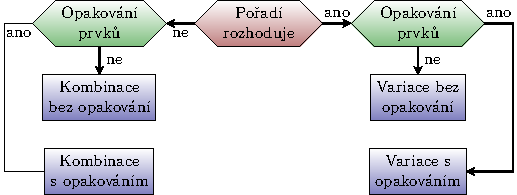
\includegraphics[width=0.7\linewidth]{mai_fig021.pdf}
        \caption{Typy výběrů. \cite[s.~201]{Musilova2009MA1}}
        \label{mai:fig021}
      \end{figure}

      Představuje-li daný výběr například volejbalové družstvo osmi děvčat (šest hráček a dvě 
      náhradnice), které bude reprezentovat v soutěži třídu osmou bé, do níž chodí \num{25} děvčat 
      a \num{18} chlapců, jedná se o výběr \(k - 8\) prvků z počtu \(n = 25\) prvků. Chlapce nelze 
      postavit do družstva volejbalistek. Každý výběr možného družstva bude představovat 
      \emph{kombinaci bez opakování}, neboť pořadí hráček nehraje roli a třeba Aničku Novákovou 
      máme ve třídě jen jednu. Budeme-li však chtít vytvářet z deseti cifer \(0, 1, \ldots, 9\) 
      trojciferná čísla, pak tyto výběry tří prvků z deseti (\(k = 3\), \(n = 10\)) jsou 
      \emph{variacemi s opakováním}. Čísla \num{125}, \num{512}, \num{251}, \num{215}, \num{521} a 
      \num{152} jsou totiž různá, a například \num{222} je také trojciferné číslo. Kombinace s 
      opakováním bychom mohli vytvářet třeba i při výběru různobarevných ponožek ze zásuvky a 
      konečně \emph{variacemi bez opakování} by mohly být dejme tomu trojbarevné signály (\(k = 
      3\)) tvořené trojicemi barevných hadříků vybíraných z \(n\) barev (pro \(n = 3\) třeba zrovna 
      z těch ponožek). Nyní bychom však rádi věděli, jak pro zadané hodnoty \(n\) a \(k\) určit 
      počet všech možných výběrů předepsaného typu. Ukážeme si to na příkladech.

      %--Šance milion-------------------------------------------------
      % !TeX spellcheck = cs_CZ
\begin{mdframed}[style=mdexam]
  \begin{example}\label{mai:exam007}
    \textbf{Šance milion}:\newline
    „Znáte nějakou jinou hru, kde můžete denně vyhrát milion?“ Tento nebo jiný, obdobně nepříliš
    vtipný reklamní slogan propaguje v televizi hru, jejímž cílem je uhodnout šestici tažených cifer
    ve správném pořadí. (Hru raději nehrajte, pravděpodobnost výhry je mizivá.) Tah se provádí
    následovně: V každém ze šesti bubnů, očíslovaných pořadovými čísly \num{1} až \num{6}, je
    připraveno deset míčků opatřených ciframi \(0, 1, \ldots, 9\). Z prvního bubnu se náhodně
    vylosuje jedna cifra (deset možností). Poté se náhodně vylosuje jedna cifra z druhého bubnu
    (opět deset možností). Možností vzniku uspořádané dvojice cifer (jedna cifra z prvního a druhá z
    druhého bubnu) je již sto (každou možnost výsledku u prvního bubnu lze kombinovat s každou
    možností výsledku z druhého bubnu). Losování pokračuje u třetího, čtvrtého, pátého a šestého
    bubnu. Celkový počet možností je \num{1e6}, tedy \textbf{milion}. (Šance získat výhru, tedy
    vyhrát milion, je ovšem pouze jedna milióntina, neboť z milionu možností je pouze jedna skutečně
    tažena.) 
  \end{example}
\end{mdframed}
      %---------------------------------------------------------------
      
      Zobecněním předchozího příkladu získáváme vzorec pro počet \textbf{variací s opakováním} 
      \emph{k}-té třídy z \(n\) prvků. Při tahu totiž záleží na pořadí bubnů a každý buben obsahuje 
      všechny cifry. Výsledky tahů z jednotlivých bubnů se tedy mohou opakovat. Pokud by bubnů bylo 
      \(k\) a v každém \(n\) různých cifer, dostali bychom pro \textbf{variace s opakováním 
      \(k\)-té třídy z \(n\) prvků} celkový počet
      \begin{equation}\label{mai:eq007}
        \boxed{V_k' = n^k}\, .
      \end{equation}

      %--Modifikovaná šance milion------------------------------------
      % !TeX spellcheck = cs_CZ
\begin{example}\label{mai:exam008}
  \textbf{Modifikovaná šance milion}:\newline
  Představme si hru z předchozího příkladu upravenou takto: K dispozici bude jen jeden buben s 
  ciframi \(0, 1, \ldots, 9\), každá cifra je v bubnu obsažena pouze jednou. Opět máme losovat 
  uspořádanou \textbf{šestici cifer}. Nyní se však jedná o \textbf{variace šesté třídy z deseti 
  prvků bez opakování}. S jediným bubnem musíme totiž provést šest losování, přičemž při každém 
  losování ubude z bubnu jedna cifra. Při prvním tahu je deset možností, při druhém již jen devět, 
  atd., při šestém již pouze pět možností. Celkem je tedy \(10 \cdot 9 \cdots 5 = \num{151200}\) 
  možností.
\end{example}
      %---------------------------------------------------------------
      
      Uvážíme-li, že v předchozím příkladu je \(n = 10\) a \(k = 6\), dostáváme pro \textbf{počet 
      variací bez opakování \(k\)-té třídy z \(n\) prvků} obecný vztah
      \begin{align}
        V_k(n) &= n(n-1)(n-2)\cdots(n-k+1)  \nonumber \\
        \shortintertext{neboli}
        V_k(n) &= \frac{n!}{(n-k)!}\, .    \label{mai:eq008}
      \end{align}
      Poznamenejme, že \(n!\) značí \textbf{faktoriál}, \(n! = n(n - 1)\cdots 3 \cdot 2 \cdot 1\). 
      Pro nulu definujeme \(0! = 1\). Je zřejmé, že při vytváření variací bez opakování musí být 
      \(k\leqq n\). Variace bez opakování \(n\)-té třídy z \(n\) prvků se nazývají 
      \textbf{permutace}. Každá z nich představuje určité uspořádání těchto \(n\) prvků. Platí
      \begin{equation}\label{mai:eq009}
        \boxed{P(n) = V_n(n) = n!}\, .
      \end{equation}
      
      Nyní odvodíme vzorec pro počet \textbf{kombinací \(k\)-té třídy z \(n\) prvků bez opakování}. 
      Již jsme si řekli, že \emph{kombinací} rozumíme takový výběr z celkového počtu \(n\) prvků, 
      který obsahuje určitých \(k\) prvků nezávisle na jejich pořadí. Představme si, že máme k 
      dispozici všechny variace bez opakování \(k\)-té třídy ze zmíněných \(n\) prvků. Vezměme 
      kteroukoli z nich. Soubor všech variací \(k\)-té třídy z \(n\) prvků však obsahuje i další 
      variace, lišící se od té naší jen pořadím prvků. Celkem je takových variací (i s tou první) 
      \(k!\) a z hlediska kombinací představují totéž. Soubor variací se tak rozpadá na podsoubory, 
      z nichž každý obsahuje \(k!\) variací lišících se navzájem pouze pořadím prvků. Každý z 
      těchto podsouborů představuje však jedinou kombinaci. Počet kombinací \(k\)-té třídy z \(n\) 
      prvků bez opakování je tedy
      \begin{equation}\label{mai:eq010}
        \boxed{C(k) = \frac{V_k(n)}{P(k)} = \frac{n!}{(n-k)!\,k!} = 
               \begin{pmatrix}
                n \\
                k
               \end{pmatrix}}\, .
      \end{equation}
      
      Pro odvození vzorce pro \textbf{kombinace s opakováním} použijeme opět příkladu.
      %--Kuličky v přihrádkách----------------------------------------
      % !TeX spellcheck = cs_CZ
\begin{mathexam}{Kuličky v přihrádkách}{exam009}
  Máme kuličky \(n\) různých barev, v každé barvě máme tolik kuliček, kolik bude potřeba. Naším
  úkolem je vytvářet výběry \(k\) kuliček. Na \textbf{pořadí barev nezáleží}, kuliček jedné barvy
  může být ve výběru libovolný počet \(0\leqq s \leqq k\). Výběry budeme vytvářet tak, že budeme
  kuličky dávat do \(n\) přihrádek, z nichž každá bude vyhrazena pro určitou barvu. Pokud tedy v
  daném výběru zrovna nebude třeba modrá kulička, bude přihrádka vyhrazená pro modrou barvu prázdná.
  Budou-li v daném výběru právě tři červené kuličky, budou umístěny v přihrádce vyhrazené pro
  červenou barvu. Vidíme, že pokud konkrétním přihrádkám přisoudíme konkrétní barvy, samotné kuličky
  by již barevné být nemusely, stačily by třeba kuličky skleněné, bezbarvé. Zůstane-li například
  přihrádka pro modrou barvu prázdná, víme, že daný výběr neobsahuje modrou barvu. Budou-li v
  přihrádce pro červenou barvu tři (bezbarvé) kuličky, víme, že daný výběr obsahuje červenou barvu
  třikrát. Příklad takové situace ukazuje následující schéma:
  
  {\centering
    \luafigure[0.9]{mai_fig033.pdf}
    \par}

  Náš úkol můžeme přeformulovat takto: Je třeba rozmístit \(k\) kuliček do \(n\) přihrádek. V každé
  přihrádce může být obecně \(s\) kuliček, kde \(0\leqq s \leqq k\), přitom celkový počet kuliček
  musí být samozřejmě stále \(k\). Můžeme si představit, že \(k\) kuliček máme položených v řadě na
  polici mezi dvěma pevnými stěnami (krajní svislé čáry v předchozím schématu) a různé způsoby
  rozmístění kuliček do přihrádek provádíme přemísťováním pohyblivých přepážek. Kdybychom například
  v předchozím schématu přesunuli druhou svislou čáru, počítáno zleva, až za první kuličku v
  přihrádce na červenou barvu, dostaneme uspořádání, při němž je v přihrádce na modrou barvu jedna
  kulička a v přihrádce na červenou barvu dvě kuličky. Tedy takto:

  {\centering
    \luafigure[0.9]{mai_fig034.pdf}
  \par}

  Mezi dvěma krajními pevnými stěnami máme tedy k dispozici \(k\) pozic pro kuličky a \((n - 1)\)
  pozic pro pohyblivé přepážky. Celkem tedy \((n + k - 1)\) pozic, na které můžeme libovolně
  rozmísťovat \(k\) kuliček a \((n - 1)\) přepážek. Do těchto \((n + k - 1)\) pozic můžeme umístit
  \(k\) kuliček \(C_k'(n)\) způsoby, kde
  \begin{equation}\label{MAI:eq011}
    \boxed{C_k'(n) =  \binom{n + k - 1}{k} = \binom{n + k - 1}{n -1}}\, .
  \end{equation}
  Na zbylé pozice již musíme umístit přepážky. Nebo naopak, nejprve umístíme \((n - 1)\) přepážek a
  potom kuličky. Výsledek je stejný, jak je vidět z předchozího vzorce. Protože jsme vytváření
  kombinací s opakováním \(k\)-té třídy z \(n\) prvků převedli na úlohu o rozmísťování kuliček do
  přihrádek, udává získaný vzorec právě počet takových kombinací. Aby měl vzorec smysl, musí platit
  \(n + k - 1 \geqq k\), tedy \(n \geqq 1\).

  Komu nevyhovuje představa kuliček v přihrádkách a má raději čísla, může uvažovat následovně: Tak
  jako je každé číslo v desítkové soustavě zapsáno pomocí cifer \(0, 1, 2, \ldots , 8, 9\), je k
  jeho zápisu ve dvojkové soustavě potřeba pouze dvou cifer, nuly a jedničky. Představme si nyní
  přepážku jako jedničku a kuličku jako nulu. Náš úkol zjistit počet všech možných způsobů rozdělení
  \(k\) kuliček do \(n\) přihrádek, ohraničených \((n+1)\) přepážkami, můžeme převést na
  ekvivalentní problém: Kolik dokážeme najít čísel, která jsou ve dvojkové soustavě zapsána právě
  \(k\) nulami a \((n + 1)\) jedničkami, požadujeme-li, aby první i poslední cifrou byla jednička?
  Odpověď je jednoduchá. Máme k dispozici \((n+k+1)\) pozic pro cifry. První a poslední pozice jsou
  pevně obsazeny jedničkami, volných pozic je tedy pouze \((n + k - 1)\). Počet všech různých
  způsobů, kterými na \(k\) z těchto pozic můžeme umístit nuly, je roven počtu kombinací \(k\)-té
  třídy z \((n + k - 1)\) prvků. Na zbylé pozice již musíme umístit jedničky. Komplementárně,
  budeme-li hledat počet všech možných způsobů, jak na \((n-1)\) pozic umístit jedničky, dostaneme
  shodný výsledek, v souhlasu se vzorcem (\ref{mai:eq010}).
\end{mathexam}
      %---------------------------------------------------------------
      
      %--Obsazování kvantových stavů----------------------------------
      % !TeX spellcheck = cs_CZ
\begin{example}\label{mai:exam010}
  \textbf{Obsazování kvantových stavů}:\newline\small
  Úloha o kuličkách a přihrádkách má přímou aplikaci v \textbf{kvantové fyzice}. Představme si, že 
  fyzikální soustava je tvořena \(k\) částicemi. Každá částice se nachází v určitém stavu, v němž 
  jí můžeme přisoudit fyzikální charakteristiky, které jsou s tímto stavem spojeny (třeba energii, 
  moment hybnosti, apod.). Jednotlivé stavy jsou pak rozlišitelné právě pomocí těchto 
  charakteristik. Dejme tomu, že přípustných stavů je \(n \geqq 1\). Problémem kvantové fyziky je 
  to, že kvantové částice jsou nerozlišitelné. Nepoznáme jednu od druhé. Je to stejné, jako bychom 
  měli \(k\) naprosto stejně vypadajících kuliček, které nemáme nijak očíslovány. Záměna dvou 
  částic (nerozlišitelných kuliček) se nepozná, nevede tedy ke změně stavu fyzikální soustavy. Pro 
  hodnoty fyzikálních charakteristik soustavy jako celku je tedy důležité jen to, kolik částic je v 
  každém z přípustných stavů. Musíme se tedy zajímat o to, kolika způsoby lze našich \(k\) 
  \textbf{nerozlišitelných částic} (kuliček) umístit do \(n\) \textbf{stavů} (přihrádek). Kvantové 
  částice jsou však dvojího druhu, \textbf{fermiony} (například elektrony, neutrony, protony, jádra 
  s lichým počtem nukleonů) a \textbf{bosony} (například fotony, mezony, jádra se sudým počtem 
  nukleonů). Rozdíl mezi nimi je ten, že bosony se „dobře snášejí“, a proto jich může být v jednom 
  stavu i více. 
  \begin{itemize}\addtolength{\itemsep}{-0.5\baselineskip}
    \item Počet možností, jak rozmístit \(k\) \textbf{bosonů} po \(n\) stavech je tedy
          \begin{equation*}
            N_{\text{boson}} = 
              \begin{pmatrix}
                n + k - 1 \\
                    k
               \end{pmatrix}
          \end{equation*}
    \item S \textbf{fermiony} je tomu jinak. \textbf{Pauliho vylučovací princip} jim zakazuje, 
          aby v daném stavu byl více než jeden fermion. Stav může být buď prázdný, nebo obsazen 
          jedním fermionem. V takovém případě musí být \(n \geqq k\) a v každé přihrádce může být 
          nejvýše jedna kulička. Situace tak odpovídá \textbf{kombinacím bez opakování \(k\)-té 
          třídy z \(n\) prvků}, tj.
          \begin{equation*}
            N_{\text{fermion}} = 
              \begin{pmatrix}
                n  \\
                k
              \end{pmatrix}
          \end{equation*}
  \end{itemize}
\normalsize
\end{example}
      %---------------------------------------------------------------
      
      Získané kombinatorické vzorce nyní použijeme při řešení základních úloh o pravděpodobnostech. 
      V každé úloze bude důležité
      \begin{itemize}
        \item definovat jev \(A\), jehož pravděpodobnost počítáme,
        \item určit počet \(N\) případů možných, tj. počet všech možných výsledků pokusu, při 
              kterém sledujeme, zda jev \(A\) nastal či nenastal,
        \item určit počet \(M\) případů příznivých, tj. počet těch výsledků daného pokusu, při 
              kterých jev \(A\) nastal.
      \end{itemize}

      %--Výhra ve sportce---	----------------------------------------
      % !TeX spellcheck = cs_CZ
\wikitextrule
\begin{example}\label{mai:exam052}
  \textbf{Výhra ve sportce}\newline\small
  Jaká je pravděpodobnost hlavní výhry ve sportce? Všichni víme, že malá, ale máme představu, jak 
  malé toto číslo je? Při sportce se losuje \(k = 6\) čísel a jedno dodatkové z celkového počtu \(n 
  = 49\) čísel. (Dříve byla čísla spojena s názvy sportů, odtud název „sportka“ .) Na pořadí čísel 
  ve výběru nezáleží, vytažené číslo se do hry nevrací. Jde tedy o \textbf{kombinace bez 
  opakování}. Hlavní výhra požaduje uhodnout všech \num{6} tažených čísel. Jev \(A\) je tedy 
  definován takto:
  
  \begin{itemize}
    \item Jev \(A\): Bude taženo právě oněch \num{6} čísel, která jsem vsadil.
          Počet možností, které při tahu sportky mohou nastat (počet případů možných), je \(N = 
          \begin{pmatrix} n \\ k\end{pmatrix} =  \begin{pmatrix} 49 \\ 6 \end{pmatrix} \). Hlavní 
          výhru představuje jediná kombinace, počet příznivých případů je proto \(M = 1\). 
          Pravděpodobnost hlavní výhry ve sportce, tj. pravděpodobnost jevu \(A\), je
          \begin{equation*}
            p(A) = \dfrac{M}{N} = \dfrac{1}{\begin{pmatrix} 49 \\ 6 \end{pmatrix}} 
                 = \dfrac{43!6!}{49!} = \dfrac{720}{49\cdot48\cdot47\cdot46\cdot45\cdot44} \simeq 
                 \num{7e-8}
                 = \SI{7e-6}{\percent}
          \end{equation*}
          Pravděpodobnost hlavní výhry je velmi malá, sedm milióntin procenta. 
    \item A o kolik lepší to bude s pravděpodobností některé z vedlejších výher? Tak třeba pátá 
          cena znamená, že je nutné ze šesti tažených čísel uhodnout libovolné tři. Jev \(A\) je 
          tedy: Ze šesti čísel, která jsme vsadili, budou v tažené kombinaci obsažena právě tři 
          libovolná z nich. Počet \(N\) zůstává stejný jako v předchozí části úlohy. Je třeba jen 
          určit \(M\). Každý příznivý případ vzniká tak, že trojice správných čísel (výběry tří ze 
          šesti) je doplněna trojicí chybných čísel (výběry tří ze čtyřiceti tří). Tedy \(M = 
          \begin{pmatrix}6 \\ 3\end{pmatrix}\begin{pmatrix} 49 - 6 \\ 3\end{pmatrix} =  
          \begin{pmatrix} 6 \\ 3\end{pmatrix}\begin{pmatrix} 43 \\ 3 \end{pmatrix}\),
          \begin{align*}
            p(A) &= \dfrac{M}{N} 
                  = \dfrac{\begin{pmatrix} 6 \\ 3\end{pmatrix}
                           \begin{pmatrix} 43 \\ 3 \end{pmatrix}}
                          {\begin{pmatrix} 49 \\ 6\end{pmatrix} }                
                  =\left(\dfrac{6!}{3!\cdot3!}\right)\left(\dfrac{43!}{40!\cdot3!}\right)
                   \left(\dfrac{43!6!}{49!}\right)                                            \\
                 &=\dfrac{120\cdot43\cdot42\cdot41\cdot720}
                         {49\cdot48\cdot47\cdot46\cdot45\cdot44\cdot36} 
                  \simeq\num{0.018}.
          \end{align*}
          Tato pravděpodobnost již zanedbatelná není, na rozdíl od finanční částky, jíž bývá 
          ohodnocena pátá cena. Sázení sportky může domácímu rozpočtu spíše ublížit.
    \item Třetí, resp. čtvrtá cena jsou, podobně jako první a pátá, definovány velmi jednoduše. Je 
          třeba uhodnout pět, resp. čtyři ze šesti tažených čísel. V případě druhé ceny hraje roli
          dodatkové číslo. Druhou cenu získává ten, kdo uhodl pět ze šesti čísel vylosovaných v 
          prvním tahu a ještě navíc číslo dodatkové, které se losuje ze zbylých \num{43} čísel, jež 
          zůstala po prvním tahu v osudí. Jev \(A\) je tedy definován takto:
          
          Ze šesti čísel, která jsem vsadil, bude při prvním tahu vylosováno libovolných pět a v 
          druhém tahu bude vylosováno právě to dodatkové číslo, které jsem vsadil. Počet případů 
          příznivých je pouze \(M = \begin{pmatrix}6 \\ 5\end{pmatrix}\), neboť šestým číslem 
          nemůže být libovolné ze \num{43} čísel, která nebyla v prvním tahu vylosována, ale 
          musí to být právě číslo dodatkové. Pravděpodobnost jevu \(A\) je
          \begin{equation*}
            p(A)  = \dfrac{M}{N} 
                  = \dfrac{\begin{pmatrix} 6  \\ 5\end{pmatrix}}
                          {\begin{pmatrix} 49 \\ 6\end{pmatrix}}
                  \simeq\num{4.2e-17}.
          \end{equation*}
          
          Pokud bychom jako jev \(A\) označili výhru jakékoliv ceny, dostaneme
          \begin{align*}
            M &= \sum_{6}^{k=3}\begin{pmatrix} 6  \\   k  \end{pmatrix}
                               \begin{pmatrix} 43 \\ 6 - k\end{pmatrix}  +
                               \begin{pmatrix} 6  \\   5  \end{pmatrix}                      \\
              &= \begin{pmatrix} 6 \\ 3\end{pmatrix}\begin{pmatrix} 43 \\ 3\end{pmatrix} +
                 \begin{pmatrix} 6 \\ 4\end{pmatrix}\begin{pmatrix} 43 \\ 2\end{pmatrix} +
                 \begin{pmatrix} 6 \\ 5\end{pmatrix}\begin{pmatrix} 43 \\ 1\end{pmatrix} +
                 \begin{pmatrix} 6 \\ 6\end{pmatrix}\begin{pmatrix} 43 \\ 0\end{pmatrix} +
                 \begin{pmatrix} 6 \\ 5\end{pmatrix},                                        \\
           p(A) &= \dfrac{\begin{pmatrix}  6 \\ 3\end{pmatrix}
                          \begin{pmatrix} 43 \\ 3\end{pmatrix}  +
                          \begin{pmatrix}  6 \\ 4\end{pmatrix}
                          \begin{pmatrix} 43 \\ 2\end{pmatrix}  +
                          \begin{pmatrix}  6 \\ 5\end{pmatrix}
                          \begin{pmatrix} 43 \\ 1\end{pmatrix}  +
                          \begin{pmatrix}  6 \\ 6\end{pmatrix}
                          \begin{pmatrix} 43 \\ 0\end{pmatrix}  +
                          \begin{pmatrix}  6 \\ 5\end{pmatrix}}
                         {\begin{pmatrix} 49 \\ 6\end{pmatrix}} =\simeq\num{0.019}.
          \end{align*}
          Všimněte si, že tento výsledek je roven součtu pravděpodobností výhry páté, čtvrté, 
          třetí, druhé a hlavní ceny. Později si tento závěr ještě připomeneme.
  \end{itemize}  
  \normalsize
\end{example}
      %---------------------------------------------------------------

      %--Losování karet-----------------------------------------------
      % !TeX spellcheck = cs_CZ
\wikitextrule
\begin{example}\label{mai:exam053}
  \textbf{Losování karet}\newline\small
    Máme karetní hru mariáš, která obsahuje celkem \num{32} karet osmi hodnot \num{7}, \num{8}, 
    \num{9}, \num{10}, J (kluk), Q (dáma), K (král), A (eso), každá hodnota je ve čtyřech barvách, 
    červené barvy jsou \(\heartsuit\) (srdce) a \(\lozenge\) (kára), černé barvy jsou \(\spadesuit\)
    (piky) a \(\clubsuit\) (kříže). Jaká je pravděpodobnost, že při náhodném vylosování deseti 
    karet budou 
    mezi nimi:
    \begin{enumerate}[label=\Alph*]
      \item právě dvě esa,
      \item alespoň dvě esa,
      \item nejvýše dvě esa,
      \item alespoň šest karet stejné barvy,
      \item právě dvě dámy a alespoň jeden kluk,
      \item právě dvě dámy nebo alespoň jeden kluk?
    \end{enumerate}

    Písmena (A) až (F) představují různé části úlohy a také zároveň definují jevy, jejichž 
    pravděpodobnost počítáme. Jedná se opět o kombinace. Nezáleží totiž na pořadí, v jakém karty 
    vytahujeme. Důležité je jen to, zda jsou vyjmenované karty ve výběru obsaženy. Počet možných 
    výsledků náhodného vylosování deseti karet z dvaatřiceti, tj. počet případů možných, je pro 
    všechny části úlohy stejný,
    \begin{equation*}
      N = \begin{pmatrix} 32 \\ 10\end{pmatrix} 
        = \dfrac{32\cdot31\cdots24\cdot23}{10\cdot9\cdots2\cdot1} = \num{64512240}.
    \end{equation*}
    
    Počítejme nyní případy příznivé pro jednotlivé jevy \(A\) až \(F\) a pravděpodobnosti těchto 
    jevů:
    \begin{equation*}
      M(A) = \begin{pmatrix} 4 \\ 2\end{pmatrix}\begin{pmatrix} 32 - 4 \\ 10 - 2\end{pmatrix}
           = \begin{pmatrix} 4 \\ 2\end{pmatrix}\begin{pmatrix} 28 \\ 8\end{pmatrix}
           = 6\cdot\dfrac{28\cdot27\cdots1}{8\cdot7\cdots2\cdot1} = \num{18648630}.
    \end{equation*}
    Jak jsme k tomuto výsledku došli? Příznivý pro daný jev je každý výběr, v němž jsou obsažena 
    právě dvě esa (libovolných barev) a žádná další esa (význam slova „právě“). Počet výběrů dvou 
    es z celkového počtu čtyř es je \(C_2(4)\), počet výběrů dalších libovolných osmi karet ze 
    zbývající části hry, která vznikne po odstranění es (nechceme, aby v příznivém výběru byla 
    další esa), je \(C_{(10-2)}(32 - 4) = C_8(28)\). Každý výběr dvojice es lze kombinovat s každým 
    výběrem zbývajících osmi karet ze zbytku hry, tj. \(M(A) = C_2(4)\cdot C_8(28)\). A to je právě
    náš předchozí výsledek. Potom:
    \begin{equation*}
      p(A) = \dfrac{M(A)}{N} 
           = \dfrac{\begin{pmatrix} 4 \\ 2\end{pmatrix}\begin{pmatrix} 28 \\ 8\end{pmatrix}}
                   {\begin{pmatrix} 32 \\ 10\end{pmatrix}}
           = \dfrac{\num{18648630}}{\num{64512240}} \simeq \num{0.29}
    \end{equation*}
    
    Aby nastal jev \(B\), požadujeme, aby v náhodném výběru deseti karet z dvaatřiceti byla alespoň 
    dvě esa. To znamená, že výběr považujeme za příznivý, obsahuje-li dvě esa libovolné barvy a osm 
    libovolných karet jiné hodnoty, nebo obsahuje tři esa libovolné barvy a sedm libovolných karet 
    jiné hodnoty, nebo obsahuje všechna čtyři esa a šest libovolných karet jiné hodnoty, \(k\) es 
    (pro \(k = 2, 3, 4\)) můžeme ze čtyř es vybrat \(\begin{pmatrix} 4 \\ k\end{pmatrix}\) způsoby.
    \(10 - k\) karet jiné hodnoty pak musíme vybírat pouze z \num{28} karet (esa je nutno 
    odstranit, aby bylo zaručeno, že „doplňkové“ karty budou mít jinou hodnotu než eso). Výběr 
    zbývajících karet lze učinit \(\begin{pmatrix} 28 \\ 10 - k\end{pmatrix}\) způsoby. Nakonec 
    tedy dostáváme
    \begin{align*}
      M(B) &=  \begin{pmatrix} 4 \\ 2\end{pmatrix}\begin{pmatrix} 28 \\ 8\end{pmatrix}
              +\begin{pmatrix} 4 \\ 3\end{pmatrix}\begin{pmatrix} 28 \\ 7\end{pmatrix}
              +\begin{pmatrix} 4 \\ 4\end{pmatrix}\begin{pmatrix} 28 \\ 6\end{pmatrix}         \\
           &=  6\cdot\dfrac{28\cdot27\cdots22\cdot21}{8\cdot7\cdots2\cdot1}
              +4\cdot\dfrac{28\cdot27\cdots23\cdot22}{7\cdot6\cdots2\cdot1}
              +1\cdot\dfrac{28\cdot27\cdots24\cdot23}{6\cdot5\cdots2\cdot1} = \num{23761530},  \\
      P(B) &= \dfrac{M(B)}{N} = \dfrac{\num{23761530}}{\num{64512240}} \simeq\num{0.37}.
    \end{align*}
    Pozn.: Někomu se předchozí výpočet může zdát příliš složitý. Nelze jej nějak zjednodušit? Co 
    kdybychom uvažovali třeba takto: Výběr dvou es již zajistí splnění požadavku. Doplňkové karty 
    tedy již pak můžeme vybírat ze třiceti karet - nebudeme tedy odstraňovat esa, protože budou-li 
    vybrána mezi doplňkovými kartami, požadavek „alespoň dvou es ve výběru“ to nenaruší. Při takové 
    interpretaci bychom dostali
    \begin{equation*}
      M(B) = \begin{pmatrix} 4 \\ 2\end{pmatrix}\begin{pmatrix} 30 \\ 8\end{pmatrix}   
           = 6\cdot\dfrac{30\cdot29\cdots24\cdot23}{8\cdot7\cdots2\cdot1}
           = \num{35117550}.
    \end{equation*}
    Vidíme, že vyšlo číslo vyšší než při předchozí úvaze. Co je tedy správně? Správně je první 
    úvaha vedoucí k nižšímu počtu příznivých případů. Při druhé úvaze jsme některé případy 
    započetli vícekrát. Zkuste přijít na to, jak se to stalo. V každém případě vidíme, že 
    kombinatorické úvahy, ať již vypadají jakkoli jednoduše, mohou být zrádné a je třeba dát si na 
    ně pozor. 
    
    Jev \(C\) podle zadání nastane, obsahuje-li náhodný výběr deseti karet nejvýše dvě esa. Znamená 
    to, že výběr je příznivý, neobsahuje-li žádné eso a obsahuje deset karet jiné hodnoty, nebo 
    obsahuje-li jedno eso a devět karet jiné hodnoty, nebo obsahuje-li dvě esa a osm karet jiné 
    hodnoty. Počet \(M(C)\) určíme analogicky jako \(M(B)\), ale pro \(k= 0, 1, 2\):
    \begin{align*}
      M(C) &=  \begin{pmatrix} 4 \\ 0\end{pmatrix}\begin{pmatrix} 28 \\ 10\end{pmatrix}
              +\begin{pmatrix} 4 \\ 1\end{pmatrix}\begin{pmatrix} 28 \\ 9\end{pmatrix}
              +\begin{pmatrix} 4 \\ 2\end{pmatrix}\begin{pmatrix} 28 \\ 8\end{pmatrix}         \\
           &=   \cdot\dfrac{28\cdot27\cdots20\cdot19}{10\cdot9\cdots2\cdot1}
              +4\cdot\dfrac{28\cdot27\cdots21\cdot20}{ 9\cdot8\cdots2\cdot1}
              +6\cdot\dfrac{28\cdot27\cdots22\cdot21}{ 8\cdot7\cdots2\cdot1} = \num{59399340}, \\
      P(C) &= \dfrac{M(C)}{N} = \dfrac{\num{59399340}}{\num{64512240}} \simeq\num{0.92}.
    \end{align*}
    
    Jev \(D\) znamená alespoň šest karet stejné barvy (připomeňme, že barvou rozumíme jednu z 
    možností \(\heartsuit\), \(\lozenge\), \(\spadesuit\), \(\clubsuit\)). Hra obsahuje osm karet 
    od každé barvy. Současně je tedy zřejmé, že karet stejné barvy může být ve výběru nejvýše osm. 
    Výběr je příznivý pro \(k = 6, 7, 8\). Obdobnou úvahou jako v předchozích případech dostáváme
    \begin{equation*}
      M = 4\cdot\sum^{8}_{k=6}
          \begin{pmatrix} 8 \\ k \end{pmatrix}\begin{pmatrix} 32 - 8 \\ 10 - k\end{pmatrix}
        = \num{1255984}.
    \end{equation*}
    
    Faktor \num{4} před celou sumou se objevuje proto, že nebylo specifikováno, která ze čtyř barev 
    má být zastoupena alespoň šesti kartami. Všechny čtyři možnosti volby barvy jsou tedy příznivé. 
    Pravděpodobnost jevu \(D\) je
    \begin{equation*}
      p(D)  = \dfrac{M(D)}{N}
            = \dfrac{4\cdot\sum^{8}_{k=6}\dfrac{8!}{k!(8-k)!}\dfrac{24!}{(10-k)!(14+k)!}}
                    {\begin{pmatrix} 32 \\ 10 \end{pmatrix}}                               
            = \dfrac{\num{1255984}}{\num{64512240}} \simeq \num{0.019}.
    \end{equation*}
    
    Případy (\(E\)) a (\(F\)) v zadání se liší pouze slůvkem „a“ a „nebo“. Uvidíme, že nejde o 
    slovíčka, ale o podstatný rozdíl. 
    
    Aby nastal jev \(E\), požadujeme, aby náhodný výběr deseti karet obsahoval právě dvě dámy a 
    alespoň jednoho kluka. Znamená to, že výběr je příznivý, obsahuje-li dvě dámy libovolné barvy a 
    současně alespoň jednoho kluka libovolné barvy. Příznivé možnosti tedy jsou:
    \begin{enumerate}
    \item  dvě dámy libovolné barvy, jeden kluk libovolné barvy, \num{7} libovolných karet, které 
           nemají hodnotu dámy ani kluka, celkem 
           \(\begin{pmatrix} 4 \\ 2 \end{pmatrix}
             \begin{pmatrix} 4 \\ 1\end{pmatrix}
             \begin{pmatrix} 32-2\cdot4 \\ 7 \end{pmatrix} = \num{8306496}\) možností,
    \item dvě dámy libovolné barvy, dva kluci libovolné barvy, \num{6} libovolných karet, které 
          nemají hodnotu dámy ani kluka, celkem 
          \(\begin{pmatrix} 4 \\ 2 \end{pmatrix}
            \begin{pmatrix} 4 \\ 2\end{pmatrix}
            \begin{pmatrix} 32-2\cdot4 \\ 6 \end{pmatrix} = \num{4845456}\) možností,
    \item dvě dámy libovolné barvy, tři kluci libovolné barvy, \num{5} libovolných karet, které 
          nemají hodnotu dámy ani kluka, celkem 
          \(\begin{pmatrix} 4 \\ 2 \end{pmatrix}
            \begin{pmatrix} 4 \\ 3\end{pmatrix}
            \begin{pmatrix} 32-2\cdot4 \\ 5 \end{pmatrix} = \num{1020096}\) možností,
    \item dvě dámy libovolné barvy, všichni čtyři kluci, \num{4} libovolné karty, které nemají 
          hodnotu dámy ani kluka, celkem 
          \(\begin{pmatrix} 4 \\ 2 \end{pmatrix}
            \begin{pmatrix} 4 \\ 4\end{pmatrix}
            \begin{pmatrix} 32-2\cdot4 \\ 4 \end{pmatrix} = \num{63756}\) možností.
    \end{enumerate}
    \begin{align*}
      M(E) &= \begin{pmatrix} 4 \\ 2 \end{pmatrix}\cdot\sum^{4}_{k=1}
              \begin{pmatrix} 4 \\ k \end{pmatrix}\begin{pmatrix} 24 \\ 8 - k \end{pmatrix}
            = 6\left[ 
                  4\begin{pmatrix} 24 \\ 7 \end{pmatrix} +
                  6\begin{pmatrix} 24 \\ 6 \end{pmatrix} +
                  4\begin{pmatrix} 24 \\ 5 \end{pmatrix} +
                   \begin{pmatrix} 24 \\ 4 \end{pmatrix}
                \right]                                                      \\ 
      M(E) &= \num{14235804},                                                \\
      p(E) &= \dfrac{M(E)}{N} = \dfrac{\num{14235804}}{\num{64512240}} \simeq \num{0.22}.
    \end{align*}
    
    Aby nastal jev \(F\), požadujeme, aby náhodný výběr deseti karet obsahoval právě dvě dámy nebo 
    alespoň jednoho kluka. Znamená to, že výběr je příznivý, obsahuje-li dvě dámy libovolné barvy a 
    jakékoli další karty, nebo obsahuje alespoň jednoho kluka a jakékoli další karty. Nyní je nutno 
    o všech možnostech pečlivě rozvažovat, abychom některé nezapočítali vícekrát. Pozor, slůvko 
    \uv{nebo} zde nemá vylučovací význam, připouští se, že mohou být splněny obě podmínky jevu 
    \(F\), tj. jak právě dvě dámy, tak alespoň jeden kluk. Příznivé možnosti jsou
    \begin{enumerate}
      \item dvě dámy libovolné barvy, žádný kluk, \num{8} libovolných karet, které nemají 
            hodnotu dámy ani kluka, celkem
            \begin{equation*}
              \begin{pmatrix} 4  \\ 2 \end{pmatrix}
              \begin{pmatrix} 4  \\ 0 \end{pmatrix}
              \begin{pmatrix} 32 - 2\cdot4 \\ 8 \end{pmatrix} = 6
              \begin{pmatrix} 24 \\ 8 \end{pmatrix},
            \end{equation*}
      \item žádná dáma, \(k\) kluků libovolné barvy pro \(k = 1, 2, 3, 4\) (alespoň jeden kluk), 
            \(10 - k\) karet, které nemají hodnotu dám y ani kluka, celkem
            \begin{equation*}
              \begin{pmatrix} 4  \\ 0 \end{pmatrix}
              \sum^{4}_{k=1}\begin{pmatrix} 4  \\ k \end{pmatrix}
                            \begin{pmatrix} 32 - 2\cdot4 \\ 10 - k \end{pmatrix} =
              \sum^{4}_{k=1}\begin{pmatrix} 4  \\ k \end{pmatrix}
                            \begin{pmatrix} 24 \\ 10 - k \end{pmatrix},
            \end{equation*}
      \item jedna dáma libovolné barvy, \(k\) kluků libovolné barvy pro \(k = 1,2, 3, 4\) (alespoň 
            jeden kluk), \(10 - k - 1\) karet, které nemají hodnotu dámy ani kluka, celkem
            \begin{equation*}
              \begin{pmatrix} 4  \\ 1 \end{pmatrix}
              \sum^{4}_{k=1}\begin{pmatrix} 4  \\ k \end{pmatrix}
                            \begin{pmatrix} 32 - 2\cdot4 \\ 10 - k - 1 \end{pmatrix} =
              4\sum^{4}_{k=1}\begin{pmatrix} 4  \\ k \end{pmatrix}
                            \begin{pmatrix} 24 \\ 9 - k \end{pmatrix},
            \end{equation*}
      \item dvě dámy libovolné barvy, \(k\) kluků libovolné barvy pro \(k = 1, 2, 3, 4\) (alespoň 
            jeden kluk), \(10 - 2 - k = 8 - k\) karet, které nemají hodnotu dámy ani kluka, celkem
            \begin{equation*}
              \begin{pmatrix} 4  \\ 2 \end{pmatrix}
              \sum^{4}_{k=1}\begin{pmatrix} 4  \\ k \end{pmatrix}
                            \begin{pmatrix} 32 - 2\cdot4 \\ 10 - k - 2 \end{pmatrix} =
              6\sum^{4}_{k=1}\begin{pmatrix} 4  \\ k \end{pmatrix}
                            \begin{pmatrix} 24 \\ 8 - k \end{pmatrix},
            \end{equation*}
      \item tři dámy libovolné barvy, k kluků libovolné barvy pro \(k = 1, 2, 3, 4\) (alespoň jeden 
            kluk), \(10 - k - 3\) karet, které nemají hodnotu dámy ani kluka, celkem
            \begin{equation*}
              \begin{pmatrix} 4  \\ 3 \end{pmatrix}
              \sum^{4}_{k=1}\begin{pmatrix} 4  \\ k \end{pmatrix}
                            \begin{pmatrix} 32 - 2\cdot4 \\ 10 - k - 3 \end{pmatrix} =
              4\sum^{4}_{k=1}\begin{pmatrix} 4  \\ k \end{pmatrix}
                            \begin{pmatrix} 24 \\ 7 - k \end{pmatrix},
            \end{equation*}
      \item všechny čtyři dámy, k kluků libovolné barvy pro \(k = 1, 2, 3, 4\) (alespoň jeden 
            kluk), \(10 - k - 4\) karet, které nemají hodnotu dámy ani kluka, celkem
            \begin{equation*}
              \begin{pmatrix} 4  \\ 4 \end{pmatrix}
              \sum^{4}_{k=1}\begin{pmatrix} 4  \\ k \end{pmatrix}
                            \begin{pmatrix} 32 - 2\cdot4 \\ 10 - k - 4 \end{pmatrix} =
              \sum^{4}_{k=1}\begin{pmatrix} 4  \\ k \end{pmatrix}
                            \begin{pmatrix} 24 \\ 6 - k \end{pmatrix},
            \end{equation*}
    \end{enumerate}
    
    Počet příznivých případů \(M(F)\) je dán součtem všech těchto možností, tedy
    \begin{equation*}
      M(F) = \begin{pmatrix}  4 \\ 2 \end{pmatrix}\begin{pmatrix} 4  \\ 0 \end{pmatrix}
             \begin{pmatrix} 24 \\ 8 \end{pmatrix} + 
              \sum^{4}_{s=0}\begin{pmatrix} 4  \\ s \end{pmatrix}
              \left[\sum^{4}_{k=1}\begin{pmatrix}  4 \\ k \end{pmatrix}
                    \begin{pmatrix} 24 \\ 10 - k - s \end{pmatrix}
              \right].
    \end{equation*}
    Všimněme si nyní výsledku. Výraz s dvojitou sumou můžeme přepsat jak
    \begin{equation*}
      \sum^{4}_{k=1}\begin{pmatrix} 4  \\ k \end{pmatrix}
        \left[\sum^{4}_{s=0}\begin{pmatrix}  4 \\ s \end{pmatrix}
              \begin{pmatrix} 24 \\ 10 - k - s \end{pmatrix}
        \right].
    \end{equation*}
    V učebnicích můžeme najít různé vzorce pro kombinační čísla, mezi nimi i vzorec
    \begin{equation*}
      \sum^{p}_{s=0}\begin{pmatrix} p \\ s \end{pmatrix}\begin{pmatrix} r \\ q - s \end{pmatrix}
        = \begin{pmatrix} r + p \\ q \end{pmatrix} \qquad\text{pro}\qquad r\geq q,\,q \geq p.
    \end{equation*}
    (Nebo si jej můžeme sami odvodit — pokuste se o to!) Pro \(p = 4\), \(r = 24\), \(q = 10 - k\), 
    \(1 \leq k \leq 4\) máme právě náš případ, takže
    \begin{equation*}
      \sum^{4}_{k=1}\begin{pmatrix} 4  \\ k \end{pmatrix}
        \left[\sum^{4}_{s=0}\begin{pmatrix}  4 \\ s \end{pmatrix}
              \begin{pmatrix} 24 \\ 10 - k - s \end{pmatrix}
        \right] = 
        \sum^{4}_{k=1}\begin{pmatrix}  4 \\ k \end{pmatrix}
                      \begin{pmatrix} 28 \\ 10 - k \end{pmatrix}.
    \end{equation*}
    Jak můžeme tento výsledek interpretovat? Jedná se o počet případů, kdy náhodný výběr deseti 
    karet z mariášové hry dvaatřiceti karet obsahuje alespoň jednu kartu pevně zvolené hodnoty (v 
    našem případě kluka), bez ohledu na to, kolik obsahuje karet ostatních hodnot. Přidáme-li počet 
    případů, kdy výběr neobsahuje žádného kluka a právě dvě dámy, dostaneme právě počet případů 
    příznivých pro jev \(F\). Pň úpravě použijeme ještě jednou vzorce
    \begin{equation*}
      \sum^{4}_{k=1}\begin{pmatrix} 4 \\ k \end{pmatrix}\begin{pmatrix} 28 \\ 10 - k\end{pmatrix}
        = \sum^{4}_{k=0}\begin{pmatrix}  4 \\ k     \end{pmatrix}
                        \begin{pmatrix} 28 \\ 10 - k\end{pmatrix} -
                        \begin{pmatrix}  4 \\ 0     \end{pmatrix}
                        \begin{pmatrix} 28 \\ 10    \end{pmatrix} =
                        \begin{pmatrix} 32 \\ 10    \end{pmatrix} -
                        \begin{pmatrix} 28 \\ 10    \end{pmatrix},
    \end{equation*}
    \begin{align*}
      M(F) &= \begin{pmatrix}  4 \\ 2 \end{pmatrix}\begin{pmatrix}  4 \\ 0 \end{pmatrix} 
              \begin{pmatrix} 24 \\ 8 \end{pmatrix} + 
              \sum^{4}_{k=1}\begin{pmatrix} 4  \\ k \end{pmatrix}
                      \left[\sum^{4}_{s=0}\begin{pmatrix}  4 \\ s \end{pmatrix}
                            \begin{pmatrix} 24 \\ 10 - k - s \end{pmatrix}
                      \right]                                                                   \\
           &= \begin{pmatrix}  4 \\ 2 \end{pmatrix}\begin{pmatrix} 24 \\ 8 \end{pmatrix} +
              \sum^{4}_{k=1}\begin{pmatrix}  4 \\ k \end{pmatrix}
                            \begin{pmatrix} 28 \\ 10 - k \end{pmatrix}                          \\
           &= \begin{pmatrix}  4 \\ 2 \end{pmatrix}\begin{pmatrix} 24 \\ 8 \end{pmatrix} + 
              \left[\begin{pmatrix}  32 \\ 10 \end{pmatrix} - 
                    \begin{pmatrix}  28 \\ 10 \end{pmatrix}
              \right]
            = \begin{pmatrix} 32 \\ 10 \end{pmatrix} - 
              \left[\begin{pmatrix} 28 \\ 10 \end{pmatrix} - 
                    \begin{pmatrix}  4 \\  2 \end{pmatrix}
                    \begin{pmatrix} 24 \\  8 \end{pmatrix}
              \right],                                                                          \\
      p(F) &= 1 - \dfrac{\begin{pmatrix} 28 \\ 10 \end{pmatrix} -
                         \begin{pmatrix}  4 \\  2 \end{pmatrix}
                         \begin{pmatrix} 24 \\  8 \end{pmatrix}
                        }
                        {\begin{pmatrix} 32 \\ 10 \end{pmatrix}}
            = 1 - \dfrac{\num{8710284}}{\num{64512240}} \simeq \num{0.86}.
    \end{align*}
    Zamysleme se ještě nad interpretací posledního výrazu pro \(M(F)\). Od počtu všech možných 
    případů se odečítá hodnota \(\begin{pmatrix} 28 \\ 10 \end{pmatrix}\) představující počet 
    situací, kdy ve výběru nebude žádný kluk, zmenšená o hodnotu \(\begin{pmatrix} 4 \\ 2 
    \end{pmatrix}\begin{pmatrix} 24 \\ 8 \end{pmatrix}\), která představuje počet situací, kdy ve 
    výběru budou právě dvě dámy a žádný kluk.
  \normalsize
\end{example}
      %---------------------------------------------------------------

      %--Sestavování čísel z cifer------------------------------------
      % !TeX spellcheck = cs_CZ
\wikitextrule
\begin{example}\label{mai:exam054}
  \textbf{Sestavování čísel z cifer}\newline\small
   Máme k dispozici libovolný počet cifer \(0, 1, \ldots, 9\). Kolik \(k\)-ciferných čísel z nich 
   můžeme sestavit? Odpověď na tuto otázku každý zná. Dvojciferná jsou čísla od \num{10} do 
   \num{99} včetně, je jich tedy \((99 - 10 + 1) = 90\). Trojciferná jsou od \(100\) do \(999\) 
   včetně, jejich počet je \((999 - 100 + 1) = 900\), \(k\)-ciferná jsou čísla od \(100\ldots0 = 
   1\cdot10^{k-1}\) do \(999\ldots9\) včetně (\(k\) devítek), jejich počet je \(9\cdot10^{k-1}\). 
   Tento výsledek bychom však měli získat i kombinatorickými úvahami. Čísla totiž dostáváme tak, že 
   z deseti cifer \(0, 1,\ldots, 9\) vytváříme variace \(k\)-té třídy s opakováním, musíme však 
   vyjmout ty možnosti, které začínají nulami. Dostáváme
   \begin{align*}
     10^k - 
       \left(
         9\cdot10^{k-2} + 9\cdot10^{k-3} + \cdots + 9\cdot10^1 + + 9\cdot10^0 + 1 
       \right)
        &= 10^k - 9\cdot\dfrac{10^{k-1} - 1}{10 - 1} - 1     \\
        &= 10^k - 10^{k-1} = 9\cdot10^{k-1}
   \end{align*}
   Jak jsme dostali odečítaný výraz v závorce? Hodnota \(9\cdot10^{k-2}\) představuje počet těch 
   výběrů cifer (s opakováním), které mají na první pozici pevnou nulu, na druhé pozici kteroukoli 
   nenulovou cifru (\num{9} možností) a na dalších \((k - 2)\) pozicích kteroukoli cifru 
   (\(10^{k-2}\) možností). Hodnota \(9\cdot10^{k-3}\) je počet těch výběrů cifer (s opakováním), 
   které mají na prvních dvou pozicích pevné nuly, na třetí pozici kteroukoli nenulovou cifru 
   (\num{9} možností) a na dalších \((k - 3)\) pozicích kteroukoli cifru (\(10^{k-2}\) možností). A 
   tak dále. Nakonec odečítáme ještě jedničku, která reprezentuje jediný výběr \(k\) cifer tvořený 
   samými nulami. Kdybychom se nyní zeptali, jaká je pravděpodobnost, že při náhodném výběru ze 
   souboru jednociferných až \(n\)-ciferných čísel vylosujeme třeba \(k\)-ciferné číslo, odpovíme 
   si již snadno: Počet případů možných je
   \begin{equation*}
     N(n) =9 + 90 + \cdots + 9\cdot10^{n-1} = 9\dfrac{10^n-1}{10 - 1} = 10^n - 1
   \end{equation*}
   počet případů příznivých je  \(M(n,k) = 9\cdot10^{k-1}\). Hledaná pravděpodobnost je tedy
   \begin{equation*}
     p(n,k) = \dfrac{9\cdot10^{k-1}}{10^n-1}.
   \end{equation*}
   Zkontrolujme si platnost získaného vzorce pro jednoduché případy, kdy ji snadno určíme přímo. 
   Pro \(n = 1\) a \(k = 1\) je vylosování jednociferného čísla jevem jistým. A skutečně, náš 
   vzorec dává
   \begin{equation*}
     p(1,1) = \dfrac{9\cdot10^0}{10^1-1} = 1.
   \end{equation*}
   Pro \(n = 2\) máme celkem \num{99} jednociferných a dvojciferných čísel, z nich jednociferných 
   je devět a dvojciferných \num{90}. Pravděpodobnost vylosování jednociferného čísla by tedy měla 
   vyjít \(9/99=1/11\) a pravděpodobnost vylosování čísla dvojciferného \(90/99=10/11\). Z našeho 
   obecného vzorce dostáváme
   \begin{equation*}
     p(2,1) = \dfrac{9\cdot10^0}{10^2-1} = \frac{9}{99} = \frac{1}{11}. \qquad
     p(2,2) = \dfrac{9\cdot10^1}{10^2-1} = \frac{90}{99} = \frac{10}{11}.
   \end{equation*}
   Jistým jevem je, že vylosujeme nějaké číslo. Skutečně také
   \begin{equation*}
     \sum_{k=1}^{n}p(n,k) = \dfrac{9}{10^n - 1}\dfrac{10^n - 1}{10 - 1} =1.
   \end{equation*}
  \normalsize
\end{example}
      %---------------------------------------------------------------

    \subsection{Sčítání a násobení - základní počty s pravděpodobnostmi}
      Někdy je třeba určit pravděpodobnosti jevů, které jsou nějakým způsobem „složeny“ z jevů
      jednodušších. Uvažujme například o jevech \(A\) a \(B\), jejichž pravděpodobnosti známe a 
      označíme je \(p(A)\) a \(p(B)\). Definujme nové jevy \(C\) a \(D\) takto:
      \begin{equation*}
        C = A \text{ a } B, \qquad D = A \text{ nebo } B.
      \end{equation*}
      Vzniká přirozená otázka, zda můžeme na základě znalosti pravděpodobností \(p(A)\) a \(p(B)\) 
      určit pravděpodobnosti \(p(C)\) a \(p(D)\). Ukazuje se, že za jistých předpokladů ano. Jako 
      obvykle nám napoví příklady.

      %--Hody kostkou a mincí - jev \(C\)-----------------------------
      % !TeX spellcheck = cs_CZ
\wikitextrule
\begin{example}\label{mai:exam055}
  \textbf{Hody kostkou a mincí - jev \(C\)}\newline\small
  Označme jako jev \(A\) „Při náhodném hodu kostkou padne šestka.“ a jako jev \(B\) \uv{Při	
  náhodném hodu mincí padne hlava.} Platí
  \begin{alignat*}{3}
    N(A) &= 6\qquad   M(A) &&=1 \qquad \Rightarrow \qquad p(A) &&= \frac{1}{6}  \\
    N(B) &= 2\qquad   M(B) &&=1 \qquad \Rightarrow \qquad p(B) &&= \frac{1}{2}  \\
  \end{alignat*}
  Jev \(C\) je definován jako \(A\) \textbf{a} \(B\), tj. „Při náhodném provedení současného hodu 
  kostkou a mincí padne na kostce šestka a na minci hlava.“ Počítejme pravděpodobnost \(p(C)\). 
  Jevy \(A\) a \(B\) jsou \textbf{nezávislé}, to znamená, že výsledek hodu kostkou neovlivní 
  výsledek hodu mincí a naopak. Počet možných výsledků současného hodu kostkou a mincí je
  \begin{equation*}
    N(C) = N(A \text{ a } B) = N(A)N(B) = 12.
  \end{equation*}
  Každý možný výsledek hodu kostkou je totiž možno kombinovat s každým možným výsledkem hodu mincí.
  Označme výsledky hodu mincí jako \(\mathcal{A}\) (hlava neboli avers) a opačný výsledek jako 
  \(\mathcal{R}\). (orel neboli revers). Výčet možných výsledků současného hodu kostkou a mincí je

  \begin{table}[h]
    \centering
    \begin{tabular}{c|rrrrrrrrrrrr}
      \textbf{kostka} & 1 & 2 & 3 & 4 & 5 & 6 & 1 & 2 & 3 & 4 & 5 & 6 \\ \hline
      \textbf{mince}  & \(\mathcal{A}\) & \(\mathcal{A}\) & \(\mathcal{A}\) & \(\mathcal{A}\) & 
                        \(\mathcal{A}\) & \(\mathcal{A}\) & \(\mathcal{R}\) & \(\mathcal{R}\) & 
                        \(\mathcal{R}\) & \(\mathcal{R}\) & \(\mathcal{R}\) & \(\mathcal{R}\) 
    \end{tabular}
    % \caption{ }
  \end{table}
  
  Příznivý případ je pouze jeden, tj. situace, kdy se výsledek \num{6} na kostce kombinuje s 
  výsledkem \(\mathcal{A}\) na minci
  
  \begin{equation*}
    M(C) = M(A)M(B) = 1.
  \end{equation*}
  \begin{equation*}
    p(C) = \dfrac{M(C)}{N(C)} = \dfrac{M(A)M(B)}{N(A)N(B)} 
         = \dfrac{M(A)}{N(A)}\cdot\dfrac{M(B)}{N(B)} = p(A)p(B).
  \end{equation*}
  \normalsize
\end{example}
      %---------------------------------------------------------------
      
      Z příkladu intuitivně chápeme, co jsou to nezávislé jevy, a usuzujeme, že obecně platí
      \begin{lemma}\label{mai:lemma003}
        \textbf{(Násobení pravděpodobností)}: Pravděpodobnost současného výskytu dvou nezávislých 
        jevů \(A\) a \(B\) (jev \(C\)) je rovna součinu jejich pravděpodobností, tj.
        \begin{equation}\label{mai:eq052}
           p(A \text{ a } B)= p(A)p(B)\qquad \text{pro } A \text{ a } B \text{ neslučitelné}
        \end{equation}
      \end{lemma}
      
      Pokusme se o přesnější definici nezávislých jevů a o odvození vztahu (\ref{mai:eq052}). 
      Označme jako \(N_A\) množinu všech možných výsledků pokusu, při němž může nastat jev \(A\), a 
      obdobně \(N_B\) množinu všech možných výsledků pokusu, při němž může nastat jev \(B\). V 
      předchozím příkladu je \(N_A = \{1, 2, 3, 4, 5, 6\}\) a \(N_B = \{\mathcal{A}, 
      \mathcal{B}\}\). Jako \(N_C\) označme množinu všech možných výsledků pokusu, při němž může 
      nastat současně jev \(A\) i jev \(B\). Jevy \(A\) a \(B\) nazveme nezávislé, jestliže
      platí \(N_C = N_A \times N_B\) (kartézský součin množin). Označíme-li obdobně \(M_A \subseteq 
      N_A\) a, \(M_B \subseteq N_B\) a \(M_C \subseteq N_C\) podmnožiny příznivých výsledků pro 
      jednotlivé jevy, je zřejmé, že také \(M_C = M_A \times M_B\). Počty prvků jednotlivých množin 
      označíme \(N(A)\), \(N(B)\), \(N(C)\) (počty možných případů) a \(M(A)\), \(M(B)\), \(M(C)\) 
      (počty příznivých případů). O konečných množinách víme, že mohutnost (počet prvků) 
      kartézského součinu množin je rovna součinu mohutností jednotlivých
      činitelů v tomto kartézském součinu. Proto
      \begin{align*}
        N(C) &= N(A)N(B),\qquad M(C) = M(A)M(B). \\
        \shortintertext{Odtud}
        p(C) &= \dfrac{M(C)}{N(C)} = \dfrac{M(A)M(B)}{N(A)N(B)} = p(A)p(B).
      \end{align*}
      Platnost tohoto vzorce lze zobecnit na nezávislé jevy \(A_1\), \(A_2\) až \(A_k\) s 
      pravděpodobnostmi \(p(A_1)\), \(p(A_2)\) až \(p(A_k)\). Pravděpodobnost jevu \(C = (A_1\text{ 
      a }A_2\text{ a }...\text{ a }A_K)\) pak je
      \begin{equation*}
        p(C) = p(A_1)p(A_2)\cdots p(A_k).
      \end{equation*}
 
      %--Hody kostkou trochu jinak - jev \(D\)------------------------
      % !TeX spellcheck = cs_CZ
\begin{mdframed}[style=mdexam]
  \begin{example}\label{mai:exam056}
    \textbf{Hody kostkou trochu jinak - jev \(D\)}\newline
    Označme nyní jako jev \(A\) „Při hodu kostkou padne šestka.“ a jako jev \(B\) „Při hodu kostkou 
    padne pětka.“ Jev \(D\) nechť je definován jako \(D = (A\text{ nebo }B)\), tj. „Při hodu kostkou 
    padne šestka nebo pětka.“ Pravděpodobnosti jevů \(A\) a \(B\) jsou \(p(A) = p(B) = 1/6\). Jevy 
    \(A\) a \(B\) jsou přitom \textbf{neslučitelné} (též vylučující se ). Nemůže
    totiž padnout pětka a šestka současně. Platí
    \begin{align*}
      N(A) &= N(B) = N(D) = N = 6                                                              \\
      M(A) &= M(B) = 1                                                                         \\
      M(D) &= M(A) + M(B) = 2,                                                                 \\
      p(D) &= \dfrac{M(D)}{N(D)} = \dfrac{M(A) + M(B)}{N}                                      \\
           &= \dfrac{M(A)}{N} + \dfrac{M(B)}{N}                                                \\
           &= p(A) + p(B) = \dfrac{2}{6} = \dfrac{1}{3}.
    \end{align*}
  \end{example}
\end{mdframed}
      %---------------------------------------------------------------
      
      Je vidět, že opět směřujeme k obecnému tvrzení:
      \begin{lemma}\label{mai:lemma004}
        \textbf{(Sčítání pravděpodobností)}: Pravděpodobnost jevů \(A\) nebo \(B\) (jev \(C\)) 
        pro neslučitelné (vylučující se) jevy \(A\) a \(B\) rovna součtu pravděpodobností jevů 
        \(A\) nebo \(B\).
        \begin{equation}\label{mai:eq053}
           p(A \text{ nebo } B)= p(A) + p(B)\qquad \text{pro } A \text{ a } B \text{ nezávislé}
        \end{equation}
      \end{lemma}
      
      Opět se pokusme o přesnější definici neslučitelných jevů a o odvození vztahu 
      (\ref{mai:eq053}). Označme, obdobně jako v předchozí úvaze o nezávislých jevech, množiny 
      \(N_A\), \(N_B\), \(N_D\) možných výsledků, při nichž mohou nastat jevy \(A\), \(B\), \(D\). 
      Předpokládejme, že \(N_A = N_B\). Pak \(N_A = N_B = N_D\), a tedy \(N(A) = N(B) = N(D) = N\). 
      Jako \(M_A\), resp. \(M_B\), resp. \(M_D\) označme podmnožiny výsledků, při nichž nastane jev 
      \(A\), resp. \(B\), resp. \(D\). Zřejmě \(M_D = M_A \cup M_B\). Pro počet prvků množiny 
      \(M_D\) platí 
      \begin{align*}
        M(D) &= M(A) + M(B) - M(A\text{ a }B).                                    \\
        \shortintertext{Pravděpodobnost jevu \(D\) je pak}
        p(D) &= \dfrac{M(D)}{N(D)} = \dfrac{M(A) + M(B) - M(A\text{ a }B)}{N} 
              = p(A) + p(B) - p(A\text{ a }B).
      \end{align*}
      
      Jevy \(A\) a \(B\) se nazývají \textbf{neslučitelné}, neboli \emph{vylučující se}, je-li 
      \(M_A \cap M_B = 0\). V takovém případě je ovšem \(M(A\text{ a }B) = 0\), a tedy
      \begin{equation*}
        p(A\text{ nebo }B) = p(A) + p(B).
      \end{equation*}
      Zobecněním na \(k\) jevů \(A_1\) až \(A_k\) po dvou neslučitelných dostáváme
      \begin{equation*}
        p(A_1\text{ nebo }\cdots\text{ nebo }A_k) = p(A_2) + p(A_2) + \cdots + p(A_k).
      \end{equation*}
      Mají-li po dvou neslučitelné jevy \(A_1\) až \(A_k\) tu vlastnost, že při daném pokusu musí 
      nastat právě jeden z nich, říkáme, že tvoří \textbf{úplný systém jevů}. Součet jejich 
      pravděpodobností je roven jedné.
      
      Jev \(\overline{A}\) se nazývá \textbf{opačný} k jevu \(A\), jestliže nastává právě tehdy, 
      když jev \(A\) nenastává. Z této definice je vidět, že jevy \(\overline{A}\) a \(A\) jsou 
      \emph{neslučitelné}. Na druhé straně je zřejmé, že jev (\(A\) nebo \(\overline{A}\)) je jevem 
      \textbf{jistým}, nastává vždy. Jeho pravděpodobnost je tedy \num{1}. Odtud
      \begin{equation}\label{mai:eq054}
        p(\overline{A}) = 1 - p(A).
      \end{equation}
      Jev \(A\) a jev \(\overline{A}\) k němu opačný tvoří úplný systém.
      
      Na závěr odstavce ještě jeden prakticky důležitý příklad.
      
      %--Bernoulliův pokus--------------------------------------------
      % !TeX spellcheck = cs_CZ
\wikitextrule
\begin{example}\label{mai:exam057}
  \textbf{Bernoulliův pokus}\newline\small
  Bernoulliův pokus spočívá v tom, že \(n\)-krát nezávisle provedeme určitý pokus, například hod 
  mincí. (V terminologii teorie pravděpodobnosti nazýváme každé takové provedení opakováním 
  pokusu.) Sledujeme, v kolika případech z těchto \(n\) opakování nastal daný jev (například jev 
  \(A\) — padne hlava). Výsledek opakování pokusu, při kterém daný jev nastal, nazveme zdarem, 
  výsledek, kdy nastal jev opačný, nezdarem. Dejme tomu, že pravděpodobnost zdaru je \(p\). (Pro 
  případ padnutí hlavy na minci je \(p = 1/2\).) Pravděpodobnost nezdaru je pak \((l - p)\).
  (V případě hodů mincí je \((1 — p) = 1/2\).) Zajímáme se o to, jaká je pravděpodobnost \(P(x)\), 
  že při \(n\) opakováních pokusu docílíme \(x\)-krát zdaru, \(x\) přitom můžeme předem volit 
  libovolně v rozmezí \(0 \leq x \leq n\). V případě hodů mincí jistě dokážeme předem odhadnout, 
  že pravděpodobnosti \(P(0)\) a \(P(n)\), tj. pravděpodobnosti toho, že nepadne hlava vůbec nebo 
  že padne hlava vždy, budou při větším počtu opakování pokusu malé a budou se blížit nule tím 
  více, čím větší bude \(n\). Naopak bychom se mohli domnívat, že pravděpodobnost \(P(n/2)\), 
  tj. že padne hlava v polovině opakování pokusu, by měla být při velkém počtu \(n\) blízká 
  \SI{100}{\percent}. Správnost tohoto našeho předběžného odhadu však posoudíme teprve poté, co si 
  odvodíme obecný vzorec pro \(P(x)\). Budeme možná překvapeni. Zvolme nejprve pevně, při kterých 
  konkrétních opakováních pokusu má dojít ke zdaru  (například při prvních \(x\)). Při ostatních 
  pak požadujeme nezdar. Protože jevy
  \begin{align*}
    A_1                &: \text{Při prvním opakování dojde ke zdaru.}                  \\
    A_2                &: \text{Při druhém opakování dojde ke zdaru.}                  \\
    \ldots             &: \ldots\ldots\ldots\ldots\ldots\ldots\ldots\ldots\ldots\ldots \\
    A_x                &: \text{Při \(x\)-tém opakování dojde ke zdaru.}               \\
    \overline{A}_{x+1} &: \text{Při \((x + 1)\)-tém opakování dojde k nezdaru.}        \\
    \ldots             &: \ldots\ldots\ldots\ldots\ldots\ldots\ldots\ldots\ldots\ldots \\
    \overline{A}_n     &: \text{Při posledním \(n\)-tém opakování dojde k nezdaru,}
  \end{align*}
  jsou nezávislé, je pravděpodobnost jevu
  \begin{itemize}
    \item \(B_1\): Při každém z prvních \(x\) opakování dojde ke zdaru a současně při každém z 
          dalších \((n — x)\) opakování dojde k nezdaru, rovna součinu pravděpodobností
          \begin{equation*}
            p(B_1) = p(A_1)p(A_2)\cdots p(A_x)p(\overline{A}_{x+1})\cdots p(\overline{A}_n) 
                   = p^x (1 - p)^{n-x}.
          \end{equation*}
  \end{itemize}
  Nám však jde o pravděpodobnost následujícího jevu
  \begin{itemize}
    \item \(B\): Právě při \(x\) opakováních pokusu (bez ohledu na to, kterých) dojde ke zdaru a 
          současně při každém ze zbývajících opakování pokusu dojde k nezdaru.
  \end{itemize}
  
  Možností výběru \(x\) opakování, při kterých dojde ke zdaru, je \(N(x) = \begin{pmatrix} n \\ 
  x\end{pmatrix}\). Pokud bychom očíslovali jednotlivé výběry \(j = 1, 2, \cdots, N(x)\), dostaneme 
  odpovídající jevy \(B_1, \cdots, B_{N(x)}\) Pravděpodobnost každého z nich je stejná a rovna 
  pravděpodobnosti jevu \(B_1\), který jsme popsali před chvílí. Tyto jevy jsou po dvou 
  neslučitelné a jev \(B\) znamená, že nastane právě jeden (kterýkoli) z nich. Pro jeho 
  pravděpodobnost tedy platí, podle pravidla pro součet pravděpodobností po dvou neslučitelných 
  jevů,
  \adjustbox{minipage=[c]{\textwidth}}{%
    \begin{equation}\label{mai:eq055}
      p(B) = P(x) = \begin{pmatrix} n \\ x\end{pmatrix}p^x (1 - p)^{n-x}.
    \end{equation}
    }
   
  Zkusme nyní prověřit správnost našeho odhadu týkajícího se hodů mincí:
  \begin{equation*}
    P(0) = \begin{pmatrix} n \\ 0\end{pmatrix} 
           \left(\dfrac{1}{2}\right)^0\left(\dfrac{1}{2}\right)^{n-0} 
         = \dfrac{1}{2^n}            \qquad
    P(n) = \begin{pmatrix} n \\ n\end{pmatrix} 
           \left(\dfrac{1}{2}\right)^n\left(\dfrac{1}{2}\right)^{n-n} 
         = \dfrac{1}{2^n}     
  \end{equation*}
  Vidíme, že náš odhad byl správný. Obě pravděpodobnosti klesají s rostoucím počtem opakování 
  pokusu k nule.  Pro jediné opakování pokusu, tj. \(n = 1\), jsou obě rovny jedné polovině, a to 
  bychom jistě také měli očekávat. 
  
  Pro \(n\) sudé nyní počítejme \(P(n/2)\). Položme \(n = 2m\):
  \begin{equation*}
    P(m) = \begin{pmatrix} 2m \\ m\end{pmatrix} 
           \left(\dfrac{1}{2}\right)^m\left(\dfrac{1}{2}\right)^{2m-m} 
         = \dfrac{(2m)!}{m!m!}\left(\dfrac{1}{2}\right)^{2m}     
  \end{equation*}

  \begin{table}[ht!]
    \centering
    \begin{tabular}{c|rrrrr}
      \(m\)    & 1 & 2 & 3 & 5 & 10  \\ \hline
      \(P(m)\) & \num{0.500} & \num{0.375} & \num{0.313} & \num{0.246} & \num{0.176}
    \end{tabular}
    % \caption{ }
  \end{table}
  
  Tady se zdá, že nás naše intuice při odhadu pravděpodobnosti \(P(n/2)\) zklamala. Tendence hodnot 
  \(P(n/2)\) je pro rostoucí \(n\) klesající. Pravděpodobnost je největší pro \(n = 2\), a to právě 
  padesátiprocentní! Zkusme ještě odhad pro velká \(n\) pomocí \textbf{Stirlingova vzorce}. Podle 
  něj pro velká \(n\) platí
  
  \begin{equation}\label{mai:eq056}
    n! \doteq \left(\dfrac{n}{e}\right)^n\sqrt{2\pi n}
  \end{equation}
  Použijeme-li jej pro výpočet P(m), dostáváme
  \begin{equation*}
    P(m)\doteq \dfrac{\left(\dfrac{2m}{e}\right)^{2m}\sqrt{4\pi m}}
     {\left(\dfrac{m}{e}\right)^m\left(\dfrac{m}{e}\right)^m\left(\sqrt{2\pi m}\right)^2}
     \left(\dfrac{1}{2}\right)^{2m} = \dfrac{1}{\sqrt{\pi m}} \longrightarrow 0
  \end{equation*}
  pro velká \(m\). Kde jsme se tedy zmýlili? Ze zkušenosti víme, že budeme-li házet mincí 
  mnohokrát, je prakticky jisté, že hlava skutečně padne zhruba v polovině případů! Problém spočívá 
  ve slovíčku zhruba. Pravděpodobnost \(P(m)\) pro \(n = 2m\) se však týká jevu, kdy hlava padne 
  přesně v polovině případů. A ta samozřejmě bude tím menší, čím větší je počet posuzovaných hodů 
  mincí. Při zvyšujícím se počtu \(n\) opakování pokusu totiž roste i počet jednotlivých možností 
  volby \(x\) a \(n\) a každou z nich tak „připadne“ menší pravděpodobnost. (Součet  
  pravděpodobností přes všechna přípustná \(x\) musí být roven jedné.) Později, v odstavci 
  \ref{mai:IchapIIIsecII}, uvidíme, že jsme nevědomky místo pravděpodobnosti odhadovali střední 
  hodnotu náhodné veličiny.
  
  Položme si ještě poslední otázku v souvislosti s Bernoulliovým pokusem: Jaká je pravděpodobnost, 
  že alespoň při jednom z \(n\) opakování pokusu nastane zdar? Pokud si po předchozím neúspěchu s 
  intuitivními odhady ještě trochu věříme, můžeme předpovídat, že tato pravděpodobnost poroste s 
  počtem opakování pokusu \(n\) a pro velmi velká \(n\) se bude blížit jedné. Musíme ji ale 
  spočítat. Někdo, kdo nečetl předchozí text příliš pečlivě, by mohl navrhnout jednoduchou úvahu: 
  Pravděpodobnost zdaru při každém opakování pokusu je \(p\), pravděpodobnost, že nastane zdar při 
  alespoň jednom z nich tedy musí být, podle pravidla pro sčítání pravděpodobností, \(np\).
  Úvaha je sice jednoduchá, ale zcela chybná. Vidíme to již ze skutečnosti, že při pevné hodnotě 
  \(p\) a dostatečně velkém \(n\) může hodnota \(np\) překročit jedničku, a to nemůže žádná 
  pravděpodobnost udělat. Kde se málo pozorný čtenář dopustil chyby, když chtěl sčítat 
  pravděpodobnosti zdaru při jednotlivých opakováních? Neuvědomil si, že pravidlo součtu 
  pravděpodobností jednotlivých jevů \(A_1\) až \(A_k\) při výpočtu pravděpodobnosti jevu 
  (\(A_1\) nebo \(A_2\) nebo \(\cdots\) nebo \(A_k\)) může použít jedině pro jevy po dvou 
  neslučitelné. Zdar při některém z opakování pokusu však nevylučuje možnost zdaru při jiném 
  pokusu. Pravidlo tedy bylo použito nesprávně. Pravděpodobnost zdaru při alespoň jednom opakování 
  pokusu snadno vypočteme pomocí jevu opačného. Opačný jev znamená, že nenastane zdar ani při 
  jednom opakování pokusu. Jednotlivá opakování jsou nezávislá, proto je pravděpodobnost nezdarů
  při všech opakováních rovna součinu pravděpodobností při jednotlivých z nich, tj. \((1 - p)^n\) . 
  Pravděpodobnost zdaru při alespoň jednom opakováni je pak doplňkem do jedničky, tedy \(1 - (1 - 
  p)^n\). Je vidět, že je tím větší, čím je větší \(n\), a její limita pro \(n\rightarrow \infty\) 
  je rovna jedné. A to je výsledek, který jsme předpověděli.
  \normalsize
\end{example}
      %---------------------------------------------------------------

    \subsection{Pravděpodobnější, než bychom čekali - podmíněná pravděpodobnost}
      Kdysi se objevila, jako nepříliš dobrý vtip, úvaha o pravděpodobnosti bomby na palubě letadla:
      Řekněme, že pravděpodobnost, že některý z pasažérů letadla má s sebou bombu, je jedna
      tisícina. Pravděpodobnost, že dva pasažéři nezávisle na sobě budou mít bombu, je pak pouze
      jedna milióntina (\(\num{e-3}\cdot\num{e-3}= \num{e-6}\)). Vezmu-li si tedy s sebou do 
      letadla svou vlastní bombu, kterou ovšem nehodlám uvést do chodu, snížím tím pravděpodobnost 
      druhé bomby na palubě na onu jednu milióntinu. Nezabývejme se nyní tím, že již první úvaha o 
      jedné milióntině je v podstatě nesprávná, i když pro případ, že pravděpodobnost \(p\), že 
      konkrétní pasažér bude mít bombu, je velmi malá, dává správný přibližný výsledek. Klíčová 
      chyba je v úvaze, že snížení pravděpodobnosti bomby na palubě můžeme napomoci vlastní bombou 
      v zavazadle. Tato úvaha nerespektuje totiž \textbf{pojem podmíněné pravděpodobnosti}, který 
      si nyní na příkladu vyložíme.
      
      %--Jak nekoupit zmetek------------------------------------------
      % !TeX spellcheck = cs_CZ
\wikitextrule
\begin{example}\label{mai:exam058}
  \textbf{Jak nekoupit zmetek}\newline\small
    Do finále soutěže o „šmejd roku“ se dostaly dva podniky, „Hvizd, s.r.o.“ a „Svist, a.s.“, které 
    zásobují trh zábavnou pyrotechnikou. První z nich kryje požadavky trhu ze \SI{70}{\percent}, 
    druhý ze zbývajících \SI{30}{\percent}. “Zjistilo se, že \SI{83}{\percent} ze všech výrobků 
    Hvizdu je vadných (nebouchají, když je to třeba, zejména však bouchají, když se to
    nejméně očekává). V případě Svistu je zmetků pouze \SI{63}{\percent}. Porota soutěže rozhodla, 
    že cenu dostane ten z obou podniků, jehož ředitel zodpoví správně následující otázky:
    \begin{enumerate}
     \item Jaká je pravděpodobnost, že náhodně zakoupená rachejtle bude fungovat tak, jak má?
     \item Jaká je pravděpodobnost, že náhodně zakoupená rachejtle, o níž se na obalu píše, že byla 
     vyrobena podnikem Hvizd, není zmetek?
     \item Jaká je pravděpodobnost, že náhodně zakoupená rachejtle, kterou se podařilo úspěšně 
     odpálit, byla vyrobena podnikem Svist?
    \end{enumerate} 
    Postupně jednotlivé úkoly vyřešíme.
    V případě a) posuzujeme pravděpodobnost jevu \(A\): „Náhodně zakoupený výrobek je funkční.“ bez 
    dalších podmínek. Jedná se o nepodmíněnou pravděpodobnost. Dejme tomu, že na trhu je v dané 
    chvíli ke koupi \(n\) rachejtlí. Z nich \SI{70}{\percent}, tj. \(\num{0.7}n\), bylo vyrobeno v 
    Hvizdu a zbytek, \(\num{0.3}n\), ve Svistu. Víme, že \SI{17}{\percent} výrobků Hvizdu je 
    funkčních, v případě Svistu je to \SI{37}{\percent}. Na trhu je tedy v tuto chvíli
    \begin{equation*}
      m = \num{0.17} - \num{0.7}n + \num{0.37}\cdot\num{0.3}n = \num{0.23}n
    \end{equation*}
    funkčních raket. Pravděpodobnost zakoupení funkční rakety je tedy
    \begin{equation*}
      p(A) = \dfrac{m}{n} = \num{0.23}.
    \end{equation*}
    Výsledek lze snadno zobecnit. Označíme-li \(p_1\) pravděpodobnost zmetku ve firmě Hvizd a 
    \(p_2\) pravděpodobnost zmetku ve firmě Svist, je pravděpodobnost funkčního výrobku ve Hvizdu 
    \((1 - p_1)\) a ve Svistu \((1 - p_2)\). Označme \(q\) podíl Hvizdu na celkové produkci. Podíl 
    Svistu je pak \((1 - q)\). Pravděpodobnost koupě funkčního výrobku je
    \begin{equation*}
      p(A) = (1 - p_1)q + (1 - p_2)(l - q) = (1 - p_2) + q(p_2 - p_1).
    \end{equation*}
    
    V úloze b) se již jedná o \textbf{podmíněnou pravděpodobnost}. Koupíme v obchodě raketu, 
    podíváme se na obal a zjistíme, že byla vyrobena ve Hvizdu. S touto dodatečnou informací chceme 
    zjistit pravděpodobnost, že až raketu rozbalíme a odpálíme, bude skutečně fungovat. Označme 
    jako jev \(B\) „Raketa byla vyrobena ve Hvizdu.“ Naším úkolem je tedy zjistit pravděpodobnost 
    jevu \(A\) (raketa bude funkční) za podmínky, že nastal jev \(B\) (byla vyrobena ve Hvizdu). 
    Tuto pravděpodobnost značíme \(p_B(A)\). Víme, že na trhu je \(qn = \num{0.7}n\) raket 
    vyrobených ve Hvizdu. To představuje pro náš další výpočet počet případů možných. Pouze \((1 - 
    p_1) = \num{0.17}\) z nich je však funkčních, počet případů příznivých je tedy \((1 - p_1)qn = 
    \num{0.17}\cdot\num{0.7}n = \num{0.119}n\). Hledaná pravděpodobnost je
    \begin{equation*}
      p_B(A) = \dfrac{(1 - p_1)qn}{qn} = 1 - p_1 = \num{0.17}
    \end{equation*}
    Všimněme si výpočtu podrobněji. \((1 - p_1)q\) představuje pravděpodobnost jevu \((A\text{ a 
    }B)\), že náhodně zakoupená raketa bude funkční a zároveň bude vyrobena ve Hvizdu. Skutečně, na 
    trhu je v dané chvíli \(n\) raket, z nich \(qn\) bylo vyrobeno ve Hvizdu a z těchto \(qn\) 
    výrobků Hvizdu je \((1 - p_1)qn\) funkčních. Proto 
    \begin{equation*}
      p(A\text{ a }B) = \dfrac{(1 - p_1)qn}{n} = (1 - p_1)q = \num{0.119}
    \end{equation*}
    (Divíte se, že tato pravděpodobnost není součinem \(p(A)p(B)\)? Nedivte se, jevy \(A\) a \(B\) 
    nejsou totiž nezávislé!). Vidíme, že platí
    \begin{equation*}
      p(A\text{ a }B) = p(B)p_B(A),
    \end{equation*}
    neboť \(q = p(B)\). Získáváme tedy vztah pro výpočet podmíněné pravděpodobnosti:
    \adjustbox{minipage=[c][32pt][c]{406pt}}{%
      \begin{equation}\label{mai:eq057}
        p_B(A) = \dfrac{p(A\text{ a }B)}{p(B)} \qquad\text{a obdobně}\qquad
        p_A(B) = \dfrac{p(A\text{ a }B)}{p(A)}.
      \end{equation}
      }
    Vzorec (\ref{mai:eq057}) jsme získali pro konkrétní příklad. Abychom byli korektní, odvoďme jej 
    obecně. Označme \(p(A)\) a \(p(B)\) pravděpodobnost jevu \(A\) a pravděpodobnost jevu \(B\), 
    \(p_B(A)\) podmíněnou pravděpodobnost jevu \(A\) za podmínky, že nastal jev \(B\), a \(p_A(B)\) 
    podmíněnou pravděpodobnost jevu \(B\) za podmínky, že nastal jev \(A\). \(p(A\text{ a }B)\) je 
    pravděpodobnost současného nastoupení jevů \(A\) a \(B\). Dejme tomu, že v celkovém počtu \(n\) 
    opakování pokusu nastal jev \(B\) \(s\)-krát. Nechť v \(t\) případech z těch, kdy nastal jev 
    \(A\), nastal také jev \(B\). Pro pravděpodobnosti pak platí
    \begin{align*}
      p(B) &= \dfrac{s}{n}, \qquad p_B(A) = \dfrac{l}{s}, \qquad p(A\text{ a }B) = \dfrac{l}{n}  \\
      p(A\text{ a }B) &= \dfrac{sp_B(A)}{n} = \dfrac{np(B)p_B(A)}{n} = p(B)p_B(A).
    \end{align*}
    Získali jsme tak obecně první část formule (\ref{mai:eq057}). Záměnou jevů \(A\) a \(B\) 
    dostaneme její druhou část. Poznamenejme, že v případě nezávislých jevů \(A\) a \(B\) je 
    samozřejmě \(p_B(A) = p(A)\) a \(p_A(B) = p(B)\). Vzorec (\ref{mai:eq057}) tak přejde v 
    pravidlo pro součin pravděpodobností nezávislých jevů.
    
    Zbývá vyřešit soutěžní úkol c). Koupili jsme raketu a odpálili ji. Fungovala. Jaká je 
    pravděpodobnost, že když se nyní podíváme na obal, zjistíme, že šlo o výrobek Svistu? Můžeme 
    již využít vztahu (\ref{mai:eq057}). Máme totiž počítat pravděpodobnost jevu \(B\) za podmínky, 
    že nastal jev \(A\). (Poznamenejme, že je-li jev \(B\) definován jako „Náhodně koupená raketa 
    pochází z Hvizdu.“, je jev „Náhodně koupená raketa pochází ze Svistu.“ jevem opačným k \(B\).) 
    Platí
    \begin{equation*}
      p_A(\overline{B}) = \dfrac{p(A\text{ a }\overline{B})}{p(A)}
                        = \dfrac{p_{\overline{B}}(A)p(\overline{B})}{p(B)}
                        = \dfrac{(1 - p_2)(1 - q)}{(1 - p_2) + q(p_2 - p_1)}
                        = \dfrac{\num{0.37}\cdot\num{0.3}}{\num{0.37} + \num{0.7}\cdot(\num{-0.2})}
                        \simeq\num{0.483}
    \end{equation*}
    Kdo chce, může snadno dospět k výsledku přímou úvahou: Na trhu je \(n\) raket, z nich funkčních 
    je \(\num{0.17}\cdot\num{0.7}n + \num{0.37} - \num{0.3}n = \num{0.23}n\). Tato hodnota je při 
    výpočtu \(p(A\text{ a }B)\)  počtem případů možných. Počet funkčních raket vyrobených Svistem 
    je \(\num{0.37}\cdot\num{0.3}n = \num{0.111}n\). To je počet případů příznivých. Hledaná 
    pravděpodobnost je tedy podílem
    \begin{equation*}
      p(A\text{ a }\overline{B}) = \dfrac{\num{0.111}n}{\num{0.23}n}\simeq\num{0.483}.
    \end{equation*}
\normalsize
\end{example}
      %---------------------------------------------------------------
      
      Nyní již snadno dokážeme přijít na chybu v úvaze o bombě v letadle, kterou jsme tento 
      odstavec uvedli. Pravděpodobnost další bomby v letadle za podmínky, že jsme tam jednu sami 
      donesli, je podmíněnou pravděpodobností. Proto je rovna podílu pravděpodobnosti, že v letadle 
      budou dvě bomby, a pravděpodobnosti, že tam bude jedna bomba, tj. \(\num{e-6}/\num{e-3} = 
      \num{e-3}\). Pocit bezpečí bychom si tedy vlastní bombou nezvýšili. Ještě abychom se báli, že 
      bouchne, zejména pokud by byla vyrobená ve Hvizdu.
      
      %--Kolika let se dožijeme?--------------------------------------
      % !TeX spellcheck = cs_CZ
\wikitextrule
\begin{example}\label{mai:exam059}
  \textbf{Kolika let se dožijeme?}\newline\small
  V rámci evidence obyvatelstva se často sledují různé údaje, které slouží k odhadům vývoje 
  mohutnosti populace. Dejme tomu, že v jihomoravském regionu zjistili, že ze statisíce dětí, které 
  se dožily pěti let, se v průměru dožije dvaceti let \num{93} tisíc a osmdesáti let \num{36} 
  tisíc. Jaká je pravděpodobnost, že vy, kteří jste se již dvaceti let dožili, se dožijete 
  osmdesátky? Označme jako jev \(A\) „Pětileté dítě se dožije osmdesáti let.“ a jako jev \(B\) 
  „Pětileté dítě se dožije dvaceti let.“ Je zřejmé, že v tomto případě platí \(p(A) = p(A\text{ a 
  }B)\) (jestliže se někdo dožil osmdesáti let, s jistotou se předtím dožil dvaceti let). My 
  posuzujeme pravděpodobnost nastoupení jevu \(A\) za podmínky, že nastal jev \(B\), tj. podmíněnou 
  pravděpodobnost \(p_B(A)\). Platí
  \begin{equation*}
    p(A)   = p(A\text{ a }B) = \num{0.36}, p(B) = \num{0.93}\Rightarrow 
    p_B(A) = \dfrac{p(A\text{ a }B)}{p(B)} = \dfrac{\num{0.36}}{\num{0.93}} \simeq \num{0.39},
  \end{equation*}
  Že ta pravděpodobnost není velká? Nezoufejte. Čísla byla fiktivní a předpovědi říkají, že již v 
  roce \num{2015} bude u nás průměrný věk žen \num{83} let, u mužů, bohužel, o něco nižší. Ještě 
  zpřesněme úvahu, která nás vede k závěru \(p(A\text{ a }B) = p(A)\). Pravděpodobnost nastoupení 
  jevu \(B\) za podmínky, že nastal jev \(A\), je v našem případě rovna jedné. Jak jsme totiž již 
  konstatovali, každý, kdo se dožil osmdesátky, se s jistotou dožil i dvacítky. Platí
  pravděpodobnost \(p_B(A)\). Platí
  \begin{equation*}
    p_A(B) = \dfrac{p(A\text{ a }B)}{p(A)} = 1 \Rightarrow p(A\text{ a }B) = p(A),
  \end{equation*}
\normalsize
\end{example}
      %---------------------------------------------------------------
      
      %--Ještě jednou bomba v letadle---------------------------------
      % !TeX spellcheck = cs_CZ
\begin{mdframed}[style=mdexam]
  \begin{example}\label{mai:exam060}
    \textbf{Ještě jednou bomba v letadle}\newline
    V úvodu odstavce jsme uvažovali o pravděpodobnosti dvou bomb v letadle jako o pravděpodobnosti
    současného nastoupení dvou nezávislých jevů s komentářem, že tato úvaha není tak docela v
    pořádku. Někdo je možná zvědavý, proč, a tak se tomuto problému budeme ještě chvíli věnovat.
    (Kdo zvědavý není, může příklad přeskočit.)
    
    Nebudeme nyní posuzovat situaci, kdy jsme do letadla přinesli bombu my sami. Zabývejme se
    přesnější odpovědí na otázku, jaká je pravděpodobnost, že v letadle budou bomby dvě, aniž bychom
    tomu sami napomáhali. Taková situace odpovídá Bernoulliovu pokusu. Samozřejmě, je třeba udělat
    jisté předpoklady, které nemusejí být zcela realistické, ale v průměru budou fungovat.
    Předpokládejme, že v letadle je \(n\) pasažérů, kteří se nijak neliší pokud jde o sklon „vzít
    bombu do letadla“. Pravděpodobnost, že daný pasažér vezme s sebou bombu, je tedy u všech stejná
    a označme ji \(p\). (To je právě ten předpoklad, který u jednotlivce není příliš realistický,
    neboť venkovská tetička jistě nemá takové nutkání vzít si spolu s husou do košíku bombu, jako
    fanatický terorista.) Hodnota \(p\) zde tedy představuje jistou „zprůměrovanou zkušenost“. Co
    přesně znamená otázka, jaká je pravděpodobnost, že v letadle je bomba? Je tím myšlena
    pravděpodobnost jevu „V letadle je alespoň jedna bomba.“ Pravděpodobnost \(P\) tohoto jevu jsme
    zadali jako jednu tisícinu (dejme tomu, že je to zase údaj odpovídající „zprůměrované zkušenosti
    “u letadel s velkým počtem cestujících). Také jsme již \(P\) počítali v závěru kapitoly
    \ref{mai:IchapIVsecIIssecIV}. Platí pro ni
    \begin{equation*}
      P = 1 - (1 - p)^n,
    \end{equation*}
    kde \(n\) je počet opakování pokusu. V našem případě nastoupení jednotlivého pasažéra do letadla
    představuje jedno opakování pokusu, takže je tento počet roven počtu pasažérů v letadle. Můžeme
    tedy určit pravděpodobnost \(p\) týkající se jednotlivého pasažéra,
    \begin{equation*}
      p = 1 - \sqrt[n]{1 - P}
    \end{equation*}
    Nyní potřebujeme znát pravděpodobnost, že v letadle jsou dvě bomby, myšleno alespoň dvě bomby.
    Označme tento jev jako \(B\). Znamená, že alespoň při dvou opakováních Bernoulliova pokusu
    nastane zdar. Jev \(\overline{B}\) k němu opačný znamená, že nastanou buď samé nezdary
    (pravděpodobnost je \((1 - p)^n\) a odpovídá hodnotě \(x = 0\) ve vzorci (\ref{mai:eq055})),
    nebo nastane právě \((n - 1)\) nezdarů a jeden zdar (pravděpodobnost je \(np(1 - p)^{n-1}\) a
    odpovídá hodnotě \(x = 1\) ve vzorci (\ref{mai:eq055})). Výsledky Bernoulliova pokusu pro různá
    \(x\) se ovšem navzájem vylučují, takže pravděpodobnost jevu \(\overline{B}\) je
    \begin{equation*}
      \boxed{p(\overline{B}) = (1 - p)^n + np(1 - p)^{n-1}}.
    \end{equation*}
    Pravděpodobnost alespoň dvou bomb v letadle (posuzovaný jev \(B\)) je pak
    \begin{equation*}
      p(B) = 1 - (1 - p)^n - np(1 - p)^{n-1}.
    \end{equation*}
    Zbývá dosadit za \(p\) pomocí známé hodnoty \(P\). Je-li \(P\) velmi malé, lze získat přibližný
    výsledek pomocí odhadů. Vzpomeneme-li si na odhady pomocí diferenciálu v odstavci
    \ref{mai:IchapVsecIII}, zjistíme, že pro hodnoty \(P\) mnohonásobně menší než \(1\) (a to je i
    náš případ) dostaneme
    \begin{equation*}
      p \simeq 1 - \left(1 - \dfrac{1}{n}P\right) = \dfrac{P}{n}.
    \end{equation*}
    Obdobně provedeme odhad pro \(p(B)\),
    \begin{align*}
      p(B) &= 1 - (1 - np) - np\left[1 - (n - 1)p\right]     \\
           &= n(n - 1)p^2\simeq \dfrac{n-1}{n}P^2\simeq P^2 = \num{e-6}.
    \end{align*}
  \end{example}
\end{mdframed}
      %---------------------------------------------------------------
      
      Nakonec ještě odvodíme obecný případ takzvané Bayesovy formule. Předpokládejme, že při
      každém opakování jistého pokusu může nastat právě jeden z \(k\) různých výsledků. Jevy \(A_1,
      A_2,\cdots, A_k\), z nichž \(j\)-tý znamená, že při pokusu byl zaznamenán \(j\)-tý výsledek, 
      jsou po dvou neslučitelné a tvoří úplný systém. Platí tedy
      \begin{equation*}
        p(A_1) + p(A_2) + \ldots  + p(A_k) = 1.
      \end{equation*}
      Označme jako \(B\) libovolný jev, který popisuje celkový výsledek pokusu. Vzhledem k 
      neslučitelnosti jevů \(A_1\) až \(A_k\) jsou neslučitelné i jevy (\(A_1\) a \(B\)) až 
      (\(A_k\) a \(B\)). Zároveň je zřejmé, že jev \(B\) lze zapsat jako
     \begin{equation*}
       B = (A_1\text{ a }B) \quad\text{nebo}\quad (A_2\text{ a }B) \qquad\ldots
       \quad\text{nebo}\quad (A_k\text{ a }B),
     \end{equation*} 
      a tedy
      \begin{equation*}
        p(B) = \sum_{j=1}^{k}p(A_j\text{ a }B) = \sum_{j=1}^{k}p(A_j)\cdot p_{A_j}(B),
      \end{equation*}
      s využitím vztahu (\ref{mai:eq057}). Současně, podle téhož vztahu, platí 
      \begin{equation*}
        p(A_j\text{ a }B) = p(B)\cdot  p_B(A_j).
      \end{equation*}
      Pomocí dvou předchozích vztahů dostáváme:
      
      \adjustbox{minipage=[c]{\textwidth}}{%
        \begin{lemma}\label{mai:lemma005}
          \textbf{(Bayesova formule):}
          \begin{equation}\label{mai:eq058}
            p_B(A_j) = \dfrac{p(A_j\text{ a }B)}{\sum_{i=1}^{k}p(A_i)\cdot p_{A_i}(B)} 
                     = \dfrac{p(A_j)\cdot p_{A_j}(B)}{\sum_{i=1}^{k}p(A_i)\cdot p_{A_i}(B)} .
          \end{equation}
        \end{lemma}
      }
      
      Bayesova formule pro výpočet podmíněné pravděpodobnosti má řadu užitečných aplikací
      
      %--Potřebují lékaři pravděpodobnost?----------------------------
      % !TeX spellcheck = cs_CZ
\begin{mdframed}[style=mdexam]
  \begin{example}\label{mai:exam061}
    \textbf{Potřebují lékaři pravděpodobnost?}\newline
    U pacienta je podezření, že trpí právě jednou ze tří chorob \(A_1\), \(A_2\) a \(A_3\).
    Pravděpodobnosti, že pacient má danou chorobu, jsou
    \begin{equation*}
      p(A_1) = \frac{1}{2},\; p(A_2) = \frac{1}{6},\; p(A_3) = \frac{1}{3},
    \end{equation*}
    tj.
    \begin{equation*}
      p(A_1) + p(A_2) + p(A_3) = 1.
    \end{equation*}
    
    Proto je předepsán ještě doplňující test, jehož výsledek bude pozitivní s pravděpodobností
    \num{0.1} v případě diagnózy \(A_1\), s pravděpodobností \num{0.2} v případě diagnózy \(A_2\) a
    \num{0.9} v případě diagnózy \(A_3\). Doplňující test byl pozitivní. Jaké jsou pravděpodobnosti
    jednotlivých nemocí \(A_1\), \(A_2\) a \(A_3\) po provedení testu?

    Označme jako jev \(B\) to, že výsledek testu je pozitivní. V zadání úlohy jsou uvedeny tyto
    podmíněné pravděpodobnosti:
    \begin{align*}
      p_1 &= p_{A_1}(B) = \num{0.1}, \\
      p_2 &= p_{A_2}(B) = \num{0.2}, \\ 
      p_3 &= p_{A_3}(B) = \num{0.9}.
    \end{align*}
    Označili jsme si je zvláštními symboly \(p_1\), \(p_2\) a \(p_3\), neboť se na ně budeme v
    dalších částech úlohy odvolávat. Podmíněné pravděpodobnosti \(p_B(A_j)\), jejichž zjištění je
    naším úkolem, jsou dány \textbf{Bayesovou formulí} (\ref{mai:eq058}). Pro \(j= 1, 2, 3\) platí
    \begin{align*}
      p_B(A_j) &= \dfrac{p(A_j)\cdot p_{A_j}(B)}{\sum_{i=1}^{k}p(A_i)\cdot p_{A_i}(B)}  \\
               &= \dfrac{p(A_j)\cdot p_{A_j}(B)}{\frac{1}{2}\cdot\num{0.1} + 
                                                \frac{1}{6}\cdot\num{0.2} + 
                                                \frac{1}{3}\cdot\num{0.9}}              \\
               &= p(A_j)\cdot p_{A_j}(B)\cdot\frac{60}{23},                             \\
      p_B(A_1) &= \frac{60}{23} \cdot\frac{1}{2}\cdot\num{0.1}                   
                = \frac{3}{23}\simeq\num{0.130},                                        \\
      p_B(A_2) &= \frac{60}{23} \cdot\frac{1}{6}\cdot\num{0.2}                   
                = \frac{2}{23}\simeq\num{0.087},                                        \\
      p_B(A_3) &= \frac{60}{23} \cdot\frac{1}{3}\cdot\num{0.9}                   
                = \frac{18}{23}\simeq\num{0.783}.
    \end{align*}
    Všimněme si, že součet získaných podmíněných pravděpodobností je roven jedné. Překvapuje nás to?
    Nemělo by, podíváte-li se, jak by dopadl součet výrazů daných Bayesovou formulí
    (\ref{mai:eq058}) přes všechna \(j\).
    
    Je vidět, že výsledek testu velmi napomohl k určení diagnózy. Pokud lékař potřebuje ještě
    spolehlivější informace, může doplňkový test provést opakovaně. Dejme tomu, že test byl proveden
    pětkrát, ve čtyřech případech byl pozitivní a v jednom negativní. Jaké jsou nyní
    pravděpodobnosti jednotlivých diagnóz \(A_1\), \(A_2\), \(A_3\)? Tento výsledek můžeme
    interpretovat jako jev \(C\): Při pětkrát opakovaném dodatečném testu bude výsledek ve čtyřech
    případech pozitivní (zdar) a v jednom případě negativní (nezdar).
    
    Vida, opět Bernoulliův pokus. Podmíněné pravděpodobnosti \(p_{A_1}(C)\), \(p_{A_2}(C)\) a
    \(p_{A_3}(C)\) jsou dány vztahem (\ref{mai:eq055}) pro pravděpodobnost výsledku Bernoulliova
    pokusu:
    \begin{align*}
      p_{A_1}(C) &= \binom{5}{4}\cdot p_1^4\cdot(1-p_1)^1   \\
                 &= 5(\num{0.1})^4(1 - \num{0.1}) = \num{4.5e-4},                   
    \end{align*}
    \begin{align*}
      p_{A_2}(C) &= \binom{5}{4}\cdot p_2^4\cdot(1-p_2)^1   \\
                 &= 5(\num{0.2})^4(1 - \num{0.2}) = \num{6.40e-3},                 
    \end{align*}
    \begin{align*}
      p_{A_3}(C) &= \binom{5}{4}\cdot p_3^4\cdot(1-p_3)^1   \\
                 &= 5(\num{0.9})^4(1 - \num{0.9}) = \num{3.2805e-1}. 
    \end{align*}
    Bayesovu formuli nyní aplikujeme na případ jevu \(C\). Pro \(j = 1, 2, 3\) je
    \begin{gather*}
      \begin{aligned}
        p_C(A_j) &= \dfrac{p(A_j)\cdot p_{A_j}(C)}{\sum_{i=1}^{k}p(A_i)\cdot p_{A_i}(C)}  \\
                 &= \dfrac{p(A_j)\cdot p_{A_j}(C)}{\frac{1}{2}\cdot\num{4.5e-4} + 
                                                  \frac{1}{6}\cdot\num{6.40e-3} + 
                                                  \frac{1}{3}\cdot\num{0.32805}}         \\
                 &= \dfrac{p(A_j)\cdot p_{A_j}(C)}{\num{0.11064}},
      \end{aligned}
    \end{gather*}
    \begin{align*}
      p_C(A_1) &= \frac{1}{2} \cdot\frac{\num{0.00045}}{\num{0.11064}}\simeq\num{0.002},     \\
      p_C(A_2) &= \frac{1}{6} \cdot\frac{\num{0.00640}}{\num{0.11064}}\simeq\num{0.010},     \\
      p_C(A_3) &= \frac{1}{3} \cdot\frac{\num{0.32805}}{\num{0.11064}}\simeq\num{0.988}.
    \end{align*}
    Nyní je o diagnóze \(A_3\) rozhodnuto v podstatě s jistotou, přestože na začátku úlohy byla její
    pravděpodobnost pouze třetinová.
  \end{example}
\end{mdframed}
      %---------------------------------------------------------------
      
      A na závěr ještě hádanky:

      %--Pohádka o Honzovi--------------------------------------------
      % !TeX spellcheck = cs_CZ
\begin{mdframed}[style=mdexam]
  \begin{example}\label{mai:exam062}
    \textbf{Pohádka o Honzovi}\newline
    Honza se vydal ke zlému černokněžníkovi vysvobodit princeznu. Černokněžník se zachechtal a
    pravil: „Princezna je za jedním z těchto tří závěsů. Uhodneš-li, za kterým, můžeš si ji odvést.
    Ne-li, zkameníš.“ Honza tentokrát neměl na pomoc hodné mravenečky ani mazanou lišku Ryšku, a tak
    se rozhodl použít svých znalostí o pravděpodobnosti. Když zjistil, že mu nepomohou, protože
    pravděpodobnosti, že princezna je za jednotlivými závěsy, jsou stejné a rovny jedné třetině,
    zvolil závěs A. Černokněžníka napadlo, že se na Honzovy znalosti o pravděpodobnostech podívá
    lépe, a aniž závěs A odhrnul, řekl: „Mám už na zahradě kamení dost, a proto ti dám jednu
    nápovědu. Ze dvou zbývajících závěsů, B a C, odhrnu ten, za kterým princezna není.“ A odhrnul
    závěs B. Princezna tam opravdu nebyla. Černokněžník řekl: „Teď se teprve rozhodni, budeš-li
    trvat na závěsu A, nebo změníš své rozhodnutí a označíš C.“ Honza přemýšlel, až se mu z hlavy
    kouřilo, a snažil se určit pravděpodobnosti, že princezna je za závěsem A, resp. C. Napadly ho
    dvě úvahy, které vypadaly docela dobře, ale vedly k různým výsledkům:
    \begin{itemize}[noitemsep]
    \item Úvaha prvá: Za závěsem B princezna není a závěsy A a C jsou rovnocenné. Pravděpodobnost,
          že je moje vyvolená ze kterýmkoli z nich, je proto \num{0.5}. Černokněžník mi tedy nijak
          nepomohl. (Nic jiného se od něj taky čekat nedalo.)
    \item Úvaha druhá: Pravděpodobnost, že princezna je za závěsem A, který jsem předem zvolil, byla
          rovna jedné třetině. Tím, že černokněžník odkryl závěs B, se však nemohla změnit. Proto
          pravděpodobnost, že najdu princeznu za závěsem C, je nyní rovna dvěma třetinám.
    \end{itemize}
    
    Poradíme Honzovi, který ze závěsů A a C má zvolit? Vzpomeneme-li si na to, co jsme před chvílí
    zjistili o podmíněných pravděpodobnostech, určitě mu poradit můžeme: Označme jako \(A\), \(B\),
    \(C\) jevy
    \begin{itemize}
      \item Jev \(A\) : Princezna je za závěsem A.
      \item Jev \(B\) : Princezna je za závěsem B.
      \item Jev \(C\) : Princezna je za závěsem C.
    \end{itemize}
    Jejich pravděpodobnosti jsou
    \begin{equation*}
      p(A) = \dfrac{1}{3}, \qquad p(B) = \dfrac{1}{3}, \qquad p(C) = \dfrac{1}{3}.
    \end{equation*}
    Víme, že Honza vybral závěs A, černokněžník tedy může odhrnout závěs B nebo C. Označme jako
    \(B'\) a \(C'\) tyto jevy.
    \begin{itemize}
      \item Jev \(B'\) : Černokněžník odhrne závěs B.
      \item Jev \(C'\) : Černokněžník odhrne závěs C.
    \end{itemize}
    Pravděpodobnosti jevů \(B'\) i \(C'\) jsou shodné a rovny jedné polovině, tj. \(p(B') = p(C') =
    1/2\) . Podle vztahu (\ref{mai:eq057}) platí
      \begin{gather*}
        \begin{aligned}
        p(A\text{ a }B') &= p(B')\cdot p_{B'}(A) = p(A)\cdot p_{A}(B') 
                          = \dfrac{1}{3}\cdot\dfrac{1}{2} = \dfrac{1}{6},  \\
        p(A\text{ a }C') &= p(C')\cdot p_{C'}(A) = p(A)\cdot p_{A}(C')
                          = \dfrac{1}{3}\cdot\dfrac{1}{2} = \dfrac{1}{6},  \\
        \shortintertext{Obdodně je}
        p(C\text{ a }B') &= p(B')\cdot p_{B'}(C) = p(C)\cdot p_{C}(B')
                          = \dfrac{1}{3}\cdot1 = \dfrac{1}{3},              \\
        p(C\text{ a }C') &= p(C')\cdot p_{C'}(C) = p(C)\cdot p_{C}(C') = 0  \\
      \end{aligned}
    \end{gather*}
    Použijeme-li těchto výsledků, dostaneme podmíněné pravděpodobnosti, že princezna je za závěsem
    A, resp. C za podmínky, že černokněžník odhrnul B:
    \begin{align*}
      p_{B'}(A) &= \dfrac{p(A\text{ a }B')}{p_{B'}} = \dfrac{1}{6}:\dfrac{1}{2} = \dfrac{1}{3},  \\
      p_{B'}(C) &= \dfrac{p(C\text{ a }B')}{p_{B'}} = \dfrac{1}{6}:\dfrac{1}{2} = \dfrac{1}{3}    
    \end{align*}
    Správná je tedy druhá Honzova úvaha. Můžeme ještě provést její kontrolu pomocí podmíněných
    pravděpodobností: Pro jev (\(A\) a \(B'\)) nebo (\(A\) a \(C'\)), utvořený ze dvou
    neslučitelných jevů pomocí spojky „nebo“, je tedy
    \begin{equation*}
      p\left((A\text{ a }B')\text{ nebo }(A\text{ a }C')\right) = \dfrac{1}{6} + \dfrac{1}{6} 
        = \dfrac{1}{3}.
    \end{equation*}
    Poslední výsledek představuje skutečnost, že princezna je za závěsem A stále s pravděpodobností
    rovnou jedné třetině, ať se černokněžník chystá odhrnout kterýkoli ze zbývajících závěsů.
  \end{example}
\end{mdframed}
      %---------------------------------------------------------------
      
      %--Může se člověk živit sázením?--------------------------------
      % !TeX spellcheck = cs_CZ
\wikitextrule
\begin{example}\label{mai:exam063}
  \textbf{Může se člověk živit sázením?}\newline\small
  Sázením sportky nebo návštěvami kasina jistě ne! To snad každý po přečtení předchozích odstavců 
  pochopil. Je však možné docela dobře „vydělat“ sázením se s lidmi. Při odhadu pravděpodobností 
  některých jevů nás často intuice zklame a výpočtem získáme hodnoty, které bychom vůbec 
  neočekávali. Tak například odhadněte bez výpočtu, jaká je pravděpodobnost, že alespoň dva lidé ve 
  vaší třídě (čítající například \(k = 23\) studentů) mají narozeniny ve stejný den. Až tento odhad 
  učiníte, zkuste počítat: Uvažme, že rok má \(n = 365\) dní. Spočítejme nejprve pravděpodobnost 
  \(P'\), že každý ze třídy má narozeniny v jiný den. Počet možných případů odpovídá variacím s 
  opakováním \(n^k\), počet případů příznivých odpovídá variacím bez opakování 
  \(\dfrac{n!}{(n-k)!}\) Máme tedy \(P'=\dfrac{n!}{(n-k)!n^k}\). Jev, který nás zajímá (tj., že 
  alespoň dva mají narozeniny ve stejný den), je jevem opačným. Hledanou pravděpodobností bude
  \begin{equation*}
    P  = 1 - P' = 1 - \dfrac{n!}{(n - k)!n^k} \simeq \num{0.5}.
  \end{equation*}
  Vsadíte-li se na večírku s třiceti a více lidmi, že se mezi vámi najdou dva s narozeninami ve 
  stejný den, je vaše vítězství již téměř zaručeno.
\normalsize
\end{example}
      %---------------------------------------------------------------
      
  \section{Náhodné veličiny}\label{mai:IchapIIIsecIII}
    Hodnota některých veličin je určena jednoznačně a „jednou provždy“. Kdykoli budeme její hodnotu 
    zjišťovat, tehdy dostaneme totéž - takže ji ani opakovaně zjišťovat nemusíme. Příkladem může 
    být skoro prázdná peněženka, ve které jsou třeba tři koruny. Dokud nebudeme pracovat a do 
    peněženky něco nepřidáme, bude hodnota veličiny \(X\) (počet korun v peněžence) stále rovna 
    \num{3}. Nemá smysl se do peněženky vůbec dívat. Pokud budeme do peněženky přidávat každý den 
    dvě koruny, také budeme vědět, jak se veličina \(X\) mění, aniž bychom se do peněženky dívali. 
    Po \(n\) dnech bude hodnota \(X = 3 + 2n\). Většina veličin, se kterými se setkáváme, se však 
    takto nechová. Jejich hodnoty se totiž často řídí náhodnými vlivy, takže při každém
    měření veličiny \(X\), tj. zjišťování její hodnoty, můžeme získat odlišný výsledek než při 
    měřeních předchozích. Uveďme některé příklady náhodných veličin.
    
    \begin{itemize}
      \item \textbf{Příklad s novorozenci}: Nechť jé veličinou \(X\) počet chlapců ve stovce 
            novorozených dětí. Zkušenost říká, že tento počet je v průměru o něco větší než 
            \num{50}, avšak pro různé skupiny po stovce novorozených dětí bude počet chlapců 
            kolísat. V jedné skupině bude \num{52}, v jiné \num{54}, někde třeba \num{60}, nebo 
            také \num{45}.
      \item \textbf{Příklad s meteoroidy a meteority}: Pro astronomy může být důležitou veličinou 
            \(X\) počet meteoroidů, které za rok dopadnou do zemské atmosféry. Jinou veličinou, 
            třeba \(K\), může být roční počet meteoritů, tj. těch meteoroidů, které v atmosféře 
            neshořely zcela, ale jejich část dopadla na povrch Země. Také tyto hodnoty budou pro 
            každý roční interval poněkud odlišné, neboť i počet dopadnuvších meteoroidů a 
            meteoritů podléhá vlivům, které se nedají přesně předvídat.
      \item \textbf{ Příklad s tlakoměrem}: Bude-li lékař měřit pacientovi tlak několikrát po 
            sobě, určitě také naměří několik různých hodnot. Krevní tlak je citlivý na náhodné 
            vlivy, třeba i na vnitřní rozrušení pacienta vyplývající ze strachu z bílého pláště.
      \item \textbf{Opakovaná měření fyzikální veličiny}: Chceme-li změřit třeba odpor elektrického
            vodiče (drátu), jedná se o měření nepřímé. Nemůžeme odpor změřit přímo, třeba jako      
            to můžeme udělat pro délku. Většinou měříme napětí \(U\) na vodiči a proud \(I\), který 
            jím protéká. Odpor pak zjišťujeme jako podíl \(R = U/I\). Změříme-li napětí i proud 
            jednou, dostaneme konkrétní hodnotu \(R\). Budeme-li měření napětí a proudu provádět 
            opakovaně, budeme dostávat poněkud odlišné hodnoty \(U\) a \(I\), a tedy i odlišné 
            hodnoty \(R\). Sledované veličiny se chovají jako náhodné. Je to způsobeno řadou 
            náhodných vlivů jak na veličiny samotné, tak na jejich měření (nepřesnost odečítání 
            údajů na stupnicích, apod.).
    \end{itemize}
  
    Při každém fyzikálním (a vlastně i nefyzikálním) experimentu máme co do činění s náhodnými 
    veličinami. Při chemických analýzách je náhodnou veličinou třeba koncentrace dané látky
    v roztoku, při experimentech biologických třeba počet uhynuvších rostlin ve stovce sazenic, 
    počet pozorovaných prvoků v zorném poli mikroskopu, výskyt vzácných ptáků ve sledované 
    lokalitě, apod. V následujících odstavcích definujeme náhodné veličiny přesněji a naučíme se s 
    nimi zacházet. Uvidíme, že zjištění určité hodnoty náhodné veličiny je otázkou jisté 
    pravděpodobnosti. Také lépe objasníme, co znamená vyjádření „v průměru“, které jsme občas v 
    předchozím textu použili a intuitivně mu jistě rozuměli.
  
    \subsection{Jak dobrý je to střelec - diskrétní rozdělení}
      Mimořádně vhodnou ukázkou náhodné veličiny je příklad se sportovním střelcem, kterým jsme
      uvedli celou kapitolu o pravděpodobnostech.
  
      %--Ještě jednou střelba, tentokrát přesněji---------------------
      % !TeX spellcheck = cs_CZ
\begin{mdframed}[style=mdexam]
  \begin{example}\label{mai:exam064}
    \textbf{Ještě jednou střelba, tentokrát přesněji}\newline
    Názvem pochopitelně nemyslíme přesnější střelbu, ale přesnější komentář, který již bude založen
    na našich znalostech o pravděpodobnosti. Dejme tomu, že podmínky střelby jsou pevně dány a
    nemění se. Patří k nim zcela jistě typ zbraně, typ terče, vzdálenost stanoviště střelce od
    terče, základní povětrnostní podmínky. Výsledky jsou pak závislé na zručnosti střelce, avšak
    jsou ovlivněny náhodným i vlivy (foukne nenadálý vítr, střelec se lekne, zatřese se mu ruka,
    náhodně se mírně pozmění vzdálenost ústí hlavně od terče nebo její sklon, apod.). Počty
    dosažených bodů daného střelce při jednom výstřelu, nebo při sérii deseti výstřelů, atd., jsou
    tedy náhodnými veličinami. Pokusme se posoudit zručnost střelce přesněji. Označme jako náhodnou
    veličinu \(X\) počet bodů dosažených při jednom výstřelu. Nejprve určeme, jakých hodnot může
    nabývat. Všichni víme, jak vypadá běžný střelecký terč. Aby však naše počty nebyly příliš
    komplikované a zdlouhavé, uvažujme o terči mnohem jednodušším. Bude tvořen vnitřním černým
    kruhem s hodnotou \(3\) body, dále středním šedivým mezikružím s hodnotou \(2\) body a vnějším
    bílým mezikružím s hodnotou \(1\) bod. Střelba do terče mimo vnější kružnici nebo zcela mimo
    terč představuje bodovou hodnotu \(0\). Při jednom výstřelu tedy může střelec docílit v principu
    jakékoli z možných hodnot

    {\centering
      \captionsetup{type=figure}
      \luafigure[0.6]{mai_fig070.pdf}
      \captionof{figure}{Ilustrace k příkladu \ref{mai:exam064}}
      \label{mai:fig070}
    \par}
    \vspace{0.5em}
    \begin{equation*}
      X\in\{x_1, x_2, x_3,x_4\} = \{0,1,2,3\}.
    \end{equation*}
    Informace, jakých hodnot může náhodná veličina nabývat, je jistě nejen cenná, ale je pro
    jakékoli další úvahy nezbytná. Sama o sobě je však nepostačující. O střelcově zručnosti se na
    základě konstrukce terče nic nedovídáme. Kvalitativně jinou informaci získáme, víme-li, že
    možných hodnot zásahu dociluje střelec s následujícími pravděpodobnostmi:

    {\centering
      \begin{tabular}{c|rrrr}
        \(x_i\)    &      0     &      1     &      2     &      3       \\
        \hline
        \(p_i\)    & \num{0.03} & \num{0.28} & \num{0.52} & \num{0.17} 
      \end{tabular}
    \par}

    Můžeme tak třeba zjistit, kolika bodů střelec zhruba docílí s vysokou pravděpodobností při pěti
    výstřelech. Tento počet je
    \begin{gather*}
      5\cdot(\num{0.03}\cdot0 + \num{0.28}\cdot1 + \num{0.52}\cdot2 + \num{0.17}\cdot3) = 
      5\cdot\num{1.83} = \num{9.15} \simeq 9.
    \end{gather*}
    Pro každou pětici výstřelů může být počet dosažených bodů samozřejmě poněkud odlišný. Veličina
    \(Y\) představující počet dosažených bodů na pět výstřelů je rovněž veličinou náhodnou. Je nám
    však jasné, že hodnota dosažených bodů v každé pětici výstřelů je s vysokou pravděpodobností
    blízká číslu 9. Co to znamená „s vysokou pravděpodobností“? Dokážeme ji spočítat? Pokusme se o
    to. Především bychom museli určit, o kolik bodů se smí dosažený počet lišit od hodnoty 9,
    abychom jej ještě považovali za „blízký číslu 9“ . Tato volba závisí čistě na naší vůli a bude
    jí odpovídat i vypočtená pravděpodobnost. Dejme tomu, že zvolíme tento interval od 7 do 11 bodů
    včetně. Jev, jehož pravděpodobnost hledáme, je tedy
    \begin{itemize}
      \item \(A\) : Při pěti výstřelech získá střelec \num{7} nebo \num{8} nebo \num{9} nebo \num{10} 
            nebo \num{11} bodů.
      \item[] Jevy
      \item \(A_j\) : Střelec získá při pěti výstřelech \(j\) bodů.
    \end{itemize}
    jsou po dvou neslučitelné, pravděpodobnost jevu \(A\) tedy bude rovna součtu pravděpodobností
    \begin{equation*}
      p(A) = \sum_{j=7}^{11} p(A_j).
    \end{equation*}
   
    Pozor! Pravděpodobnosti \(p(Aj)\) jsou odlišné od pravděpodobností zadaných v první tabulce. Ta
    se totiž týká pěti výstřelů, zatímco tabulka \ref{mai:tab004} je pro jeden výstřel. Musíme tedy
    určit pravděpodobnosti \(p(A_j)\). K tomu je třeba zjistit všechny možnosti, jak docílit součtu
    bodů \(j\) pomocí pěti sčítanců nabývajících hodnot \num{0} až \num{3}. Soupis je v následující
    tabulce. Tabulka uvádí různé rozklady součtu na sčítance, počet případů, jak se tento rozklad
    realizuje (různé pořadí dosažených bodů při jednotlivých výstřelech) a pravděpodobnosti
    jednotlivých rozkladů zaokrouhlené na tři platná místa.

    Jak jsme spočítali pravděpodobnosti jednotlivých rozkladů? Dejme tomu, že počet bodů dosažených
    při pěti výstřelech je \(j\). Nechť \(j = j_1 + j_2 + j_3 + j_4 + j_5\) je rozklad hodnoty \(j\)
    na součet pěti sčítanců. Čísla \(j_1\) až \(j_5\) se pohybují od \num{0} do \num{3}, mohou být i
    shodná. Například jeden z možných rozkladů bodového součtu \(j = 9\) je \(9 = 3 + 2 + 2 + 1 +
    1\). Pravděpodobnost, že při pěti nezávislých výstřelech budou jednotlivé zásahy činit \(j_1\),
    \(j_2\), \(j_3\) , \(j_4\)a \(j_5\) bodů, je
    \begin{equation*}
      p_{j1}p_{j2}p_{j3}p_{j4}p_{j5}.
    \end{equation*}
    Pro případ zvoleného konkrétního rozkladu čísla \num{9} je to \(p_3p_2^2p_1^2\) - Zásahy s
    bodovým ziskem \(j_1\) až \(j_5\) mohou být realizovány v různých pořadích (například \(\num{3}
    + \num{2} + \num{2} + \num{1} + \num{1} = \num{2} + \num{3} + \num{2} + \num{1} + \num{1}
    =\ldots\), atd.). Označme počet všech takových pořadí \(n_{j_1\ldots j_5}\). (Pro \(j = \num{3}
    + \num{2} + \num{2} + \num{1} + \num{1}\) je \(n_{32211} = \binom{5}{2}\binom{3}{2} = 30\): Dvě
    z pěti pozic pro umístění dvou dvojek lze vybrat \(\binom{5}{2}\) způsoby, ze zbývajících tří
    pozic lze dvě pro umístění jedniček vybrat \(\binom{3}{2}\) způsoby a na trojku zbude poslední
    pozice.) Pravděpodobnost \(p_{j_1\ldots j_5}\) daného rozkladu čísla \(s\) pak je
    \begin{equation*}
      p_{j_1\ldots j_5} = n_{j_1\ldots j_5}p_{j_1}p_{j_2}p_{j_3}p_{j_4}p_{j_5}
    \end{equation*}

    {\centering
    \resizebox{1\textwidth}{!}{%
    \begin{tabular}{c|rrrr}
      součet \(j\)& sčítance   &    počet   & ppst rozkladu & \(p(A_j)\) \\ \hline
            7     & 3+3+1+0+0  & \num{30}   & \num{2.18e-4} & \num{0.102} \\
                  & 3+2+2+0+0  & \num{30}   & \num{1.24e-3} & \\
                  & 3+2+1+1+0  & \num{60}   & \num{1.25e-2} & \\
                  & 3+1+1+1+1  & \num{5}    & \num{5.22e-3} & \\
                  & 2+2+2+1+0  & \num{20}   & \num{2.36e-2} & \\
                  & 2+2+1+1+1  & \num{10}   & \num{5.94e-2} & \\ \hline
            8     & 3+3+2+0+0  & \num{30}   & \num{4.06e-4} & \num{0.185} \\
                  & 3+3+1+1+0  & \num{30}   & \num{2.04e-3} & \\
                  & 3+2+2+1+0  & \num{60}   & \num{2.32e-2} & \\
                  & 3+2+1+1+1  & \num{20}   & \num{3.88e-2} & \\
                  & 2+2+2+2+0  & \num{5}    & \num{1.10e-2} & \\
                  & 2+2+2+1+1  & \num{10}   & \num{1.10e-1} & \\ \hline
            9     & 3+3+3+0+0  & \num{10}   & \num{4.42e-5} & \num{0.238} \\
                  & 3+3+2+1+0  & \num{60}   & \num{7.57e-3} & \\
                  & 3+3+1+1+1  & \num{10}   & \num{6.34e-3} & \\
                  & 3+2+2+2+0  & \num{20}   & \num{1.43e-2} & \\
                  & 3+2+2+1+1  & \num{30}   & \num{1.08e-1} & \\
                  & 2+2+2+2+1  & \num{5}    & \num{1.02e-1} & \\ \hline
          10      & 3+3+3+1+0  & \num{20}   & \num{8.25e-4} & \num{0.215} \\
                  & 3+3+2+2+0  & \num{30}   & \num{7.03e-3} & \\
                  & 3+3+2+1+1  & \num{30}   & \num{3.53e-2} & \\
                  & 3+2+2+2+1  & \num{20}   & \num{1.34e-1} & \\
                  & 2+2+2+2+2  & \num{1}    & \num{3.80e-2} & \\ \hline
          11      & 3+3+3+2+0  & \num{20}   & \num{1.53e-3} & \num{0.133} \\
                  & 3+3+3+1+1  & \num{10}   & \num{3.85e-3} & \\
                  & 3+3+2+2+1  & \num{30}   & \num{6.56e-2} & \\
                  & 3+2+2+2+2  & \num{5}    & \num{6.21e-2} & \\ \hline
    \end{tabular}}
    \captionsetup{type=table} 
    \captionof{table}{Tabulka rozkladů pro daný součet bodů: ve sloupci \uv{počet} je uveden počet 
                      kombinací, které vedou ke stejnému nástřelu (sloupec \uv{součet}) a s daným
                      bodovým ohodnocením (sloupec \uv{sčítanec})}
    \label{mai:tab004}
    \par}
    \vspace{\baselineskip}

    Pro rozklad \(\num{9} = \num{3} + \num{2} + \num{2} + \num{1} + \num{1}\) je (výsledek viz také
    v tabulce)
    \begin{equation*}
      p_{32211} =30\cdot p_3p_2^2p_1^2 = \num{30}\cdot\num{0.17}\cdot\num{0.52}^2\cdot\num{0,282} 
                \simeq \num{0.108}.
    \end{equation*}
    Pravděpodobnost \(p(A_j)\) je součtem pravděpodobností jednotlivých rozkladů čísla \(j\).
    Konečně pravděpodobnost, že střelec dosáhne bodového výsledku \(y \in [7, 11]\), je rovna součtu
    pravděpodobností \(p(A_j)\) pro \(j = 7, 8, 9, 10, 11\). Tato hodnota je \num{0.873}, tedy
    opravdu poměrně vysoká, jak jsme očekávali. Také bychom mohli říci, že střelec dosahuje při
    každé pětici výstřelů „v průměru“ \num{9} bodů, a tedy při jednom výstřelu „v průměru“ \num{1.8}
    bodů. Pokud bychom „průměrnou hodnotu“ jednoho výstřelu počítali i pro jiný počet výstřelů než
    pro pět, budeme dostávat čísla, která budou hodnotě \num{1.8} velmi blízká.
  \end{example}
\end{mdframed}
      %---------------------------------------------------------------
    
    Položme si ještě otázku, jak můžeme zjistit pravděpodobnosti, se kterými střelec dosáhne při
    jednom výstřelu daného počtu bodů. Prakticky to lze provést jedině tak, že střelec mnohokrát
    vystřelí na terč a jeho zásahy budou při tom zaznamenávány. Dejme tomu, že vystřelil \(n\)-krát 
    a že počet výstřelů, při nichž byl bodový zisk \(j\) bodů ( \(j = 0, 1, 2, 3\)), byl \(n_j\). 
    Pak pro pravděpodobnost bodového zisku \(j\) bodů při jednom výstřelu je \(p_j = n_j/n\). 
    Kdybychom provedli skutečný experiment se střelcem a počítali pravděpodobnosti \(p_j\) znovu a 
    znovu po každém dalším výstřelu, viděli bychom, že pro malé hodnoty \(n\) nejprve kolísají a 
    pro rostoucí \(n\) se začínají ustalovat a již kolísají velmi málo. Tímto postupem bychom je 
    mohli určit tak, aby byly pro náš účel rozumně přesné - třeba s přesností na dvě platná místa. 
    Rozumnou přesností je zde myšlena skutečnost, že nemá smysl chtít zjišťovat pravděpodobnost 
    třeba na šest platných míst. Vzhledem k principiální přítomnosti náhodných vlivů se kolísání 
    pravděpodobností nikdy nezbavíme, takže platná místa na pozicích, kde se kolísání trvale 
    projevuje již bez ohledu na zvyšující se \(n\), nemají smysl.
    
    V příkladu \ref{mai:exam064} jsme se již velmi těsně přiblížili důležitým charakteristikám, 
    které určují náhodnou veličinu a jsou přitom matematicky korektně definovány. Viděli jsme, že 
    známe-li jen hodnoty, kterých může náhodná veličina nabývat, nemůžeme o ní říci již nic 
    dalšího. Známe-li však ještě pravděpodobnosti, se kterými jednotlivých hodnot nabývá, můžeme o 
    ní získat již velmi mnoho informací.

    \adjustbox{minipage=[c]{\textwidth}}{%
      \textbf{Náhodnou veličinou s diskrétním rozdělením} nazýváme takovou veličinu \(X\), která
      může nabývat konečně mnoha různých hodnot \((x_1, x_2, \ldots, x_k)\) s pravděpodobnostní
      \((p_1, p_2, \ldots, p_k)\) popřípadě spočetně mnoha hodnot \((x_1, x_2, \ldots)\) s 
      pravděpodobnostmi \((p_1, p_2, \ldots)\).
      }

    Jevy \(A_j\) \uv{Veličina \(X\) nabývá hodnoty \(x_j\)}, jsou po dvou neslučitelné. Platí
    \begin{equation*}
      \sum_{j=1}^{k}p_j = 1, \qquad\text{resp.}\qquad \sum_{j=1}^{k=\infty}p_j = 1
    \end{equation*}
    Pokud jde o druhý z obou případů, nebudeme se jím prozatím zabývat. Soubor všech dvojic
    \begin{equation*}
      \left\lbrace(x_j, p_j)\right\rbrace,\qquad j = 1, 2, \ldots, k,
    \end{equation*}
    se nazývá \textbf{rozdělení} náhodné veličiny \(X\). Můžeme je znázornit i graficky.

    %--Bernoulliovo (binomické) rozdělení---------------------------
    % !TeX spellcheck = cs_CZ
\begin{mdframed}[style=mdexam]
  \begin{example}\label{mai:exam065}
    \textbf{Bernoulliovo (binomické) rozdělení}\newline
    Představme si opět Bernoulliův pokus o \(n\) opakováních a pravděpodobností zdaru při jednom
    opakování rovnou \(p\) (kapitola \ref{mai:IchapIVsecIIssecIV}). Náhodnou veličinu \(X\)
    definujme jako počet zdarů při tomto pokusu. Tato veličina nabývá všech celočíselných hodnot
    \(x_j = j, 0 \leq j \leq n\), přitom hodnoty \(j\) nabývá s pravděpodobností určenou vztahem
    (\ref{mai:eq055}), v němž za \(x\) dosadíme \(j\). 
    
    {\centering
      \captionsetup{type=figure}
      \luafigure[1]{mai_fig044.pdf}
      \captionof{figure}{Bernoulliovo rozdělení
      \cite[s.~229]{Musilova2009MA1}
      \label{mai:fig044}}
    \par}
    
    Získané rozdělení je tedy
    \begin{equation*}
      \lbrace j,p_j\rbrace, \quad\text{kde}\quad p_j = \binom{n}{j}p^j(1 - p)^{n-j}.
    \end{equation*}
    Graf Bernoulliova rozdělení, které je často nazýváno také binomickým, je na obrázku 
    \ref{mai:fig044} pro \(n = 15\) a \(p = 1/2\) (červený asterisk).
    
    Z grafu je názorně vidět, co to znamená, že některé hodnoty veličiny \(X\) jsou více a jiné méně 
    pravděpodobné. Hodnota \(x_i\), veličiny \(X\), které odpovídá největší pravděpodobnost \(p_i\), 
    se nazývá nejpravděpodobnější hodnota. V případě Bernoulliova rozdělení na obrázku 
    \ref{mai:fig044} jsou takové hodnoty dvě, konkrétně \(x_7 = 7\) a \(x_8 = 8\).
    
      \begin{lstlisting}[style=luaCPPStyle, caption={PPST001.m}]
        citatel= factorial(n);
        jmenovatel= factorial(n-j).*factorial(j);
        binom = citatel./jmenovatel;
        f = binom.*p.^j.*(1-p).^(n-j);
      \end{lstlisting}
  \end{example}
\end{mdframed}
    %---------------------------------------------------------------
    
    Nyní definujeme další charakteristiky náhodné veličiny. Těmi základními jsou, kromě již 
    definované \emph{nejpravděpodobnější hodnoty}, ještě \textbf{střední hodnota}, \textbf{rozptyl} 
    (popřípadě jeho odmocnina, zvaná \textbf{střední kvadratická} nebo \textbf{směrodatná 
    odchylka}), \textbf{medián}, popřípadě \textbf{P-kvantil}. Pojem střední hodnoty jsme již v 
    podstatě vybudovali v příkladu se střelcem. Nyní postup zobecníme. Předpokládejme, že při 
    velkém počtu \(n\) měření náhodné veličiny \(X\) naměříme různé hodnoty \((x_1, x_2, \ldots, 
    x_k)\) tak, že hodnota \(x_1\) byla naměřena \(n_1\)-krát, hodnota \(x_2\) \(n_2\)-krát, atd., 
    až hodnota \(x_k\) \(n_k\)-krát. Je zřejmé, že součet četností \(n_1\), \(n_2\), až \(n_k\) 
    jednotlivých hodnot musí být roven celkovému počtu měření \(n\) a že podíly
    \begin{equation*}
      p_1 = \dfrac{n_1}{n}, \qquad p_2 = \dfrac{n_2}{n}, \qquad \ldots, \qquad p_k = \dfrac{n_k}{n},
    \end{equation*}
    představují pravděpodobnosti jednotlivých hodnot veličiny \(X\). Tím je zadáno její rozdělení,
    které ji plně charakterizuje. Položme si však otázku, zda by se veličina \(X\) přece jen nedala
    charakterizovat jedinou hodnotou, která by všechny různě pravděpodobné hodnoty v jistém
    smyslu „zastupovala“. Kdybychom třeba takto měřili délku stolu, jistě bychom na otázku „Kolik
    měří stůl?“ neodpovídali tím, že bychom tazateli předložili získané rozdělení, i když by taková
    odpověď byla nejvýstižnější. Určitě bychom uvedli jedinou hodnotu. Ale jakou? I laika napadne,
    že by takovou reprezentativní hodnotou mohl být aritmetický průměr naměřených hodnot \(x_1\) až
    \(x_k\). Bylo by ale správné vzít jen prostý aritmetický průměr těchto různých hodnot a nebrat 
    ohled na skutečnost, že některé byly naměřeny s větší a jiné s menší četností? Nikoliv. 
    Reprezentativní hodnota veličiny \(X\) nemá zastupovat jen naměřené hodnoty, ale celé 
    rozdělení. Určitá hodnota \(x_j\) bude mít tím větší vliv na reprezentativní hodnotu, s čím 
    větší četností byla naměřena. Protože byla naměřena \(n_j\)-krát, musíme ji také tolikrát do 
    aritmetického průměru započíst.Získáváme tak \textbf{vážený aritmetický průměr} naměřených 
    hodnot, neboli \emph{střední hodnotu}
    
    \adjustbox{minipage=[c]{\textwidth}}{%
      \begin{equation}\label{mai:eq059}
        \left\langle x \right\rangle = \dfrac{n_1x_1 + n_2x_2 + \cdots + n_kx_k}{n}
          = p_1x_1 + p_2x_2 + \cdots + p_kx_k 
          = \sum_{j=1}^{k}p_jx_j.
      \end{equation}
      }
      Součet všech pravděpodobností \(p_1 + p_2 + \cdots + p_k\) je pochopitelně \textbf{roven 
      jedné}.

    %--Střední hodnota Bernoulliova rozdělení-----------------------
    % !TeX spellcheck = cs_CZ
\begin{mdframed}[style=mdexam]
  \begin{example}\label{mai:exam066}
    \textbf{Bernoulliovo (binomické) rozdělení}\newline
    Pro střední hodnotu Bernoulliova rozdělení platí
    \begin{equation*}
      \langle j \rangle = \sum_{j=0}^{n}j\cdot p_j
        = \sum_{j=1}^{n}j\begin{pmatrix} n \\ j \end{pmatrix}p^j(1-p)^{n-j} = np.
    \end{equation*}
    
    Tento vztah lze dokázat matematickou indukcí vzhledem k proměnné \(n\). Na tomto místě nebudeme
    důkaz provádět pro jeho poměrnou zdlouhavost. Každý jej však může zvládnout. Vzpomeňme si v tuto
    chvíli na náš chybný intuitivní odhad v kapitole \ref{mai:IchapIVsecIIssecIV}, v níž jsme
    poprvé hovořili o Bernoulliově pokusu v souvislosti s hody mincí. Chybně jsme tam odhadli
    pravděpodobnost, že při \(n\) opakováních pokusu nastane v polovině z nich zdar. Tato chyba
    vznikla v důsledku naší zkušenosti, že když budeme mincí vícekrát házet, padne hlava (zdar)
    skutečně zhruba v polovině případů. Vidíme nyní, že \(n/2\) reprezentuje střední hodnotu náhodné
    veličiny \(X =\) \textbf{počet zdarů při \(n\) hodech mincí}. A to naší zkušenosti již odpovídá.
  \end{example}
\end{mdframed}
    %---------------------------------------------------------------
    
    Posuďme nyní situaci, kdy náhodná veličina \(Y\) je funkcí náhodné veličiny \(X, Y = f(X)\).
    V takovém případě má rozdělení veličiny \(Y\) tvar
    \begin{equation*}
      \left\lbrace (f(x_j), p_j)\right\rbrace, \qquad j = 1, 2, \ldots, k.
    \end{equation*}
    Pravděpodobnost hodnoty \(f(x_j)\) je stejná jako pravděpodobnost hodnoty \(x_j\). Pro výpočet
    střední hodnoty veličiny \(Y\) pak platí
    \begin{equation}\label{mai:eq060}
      \left\langle y \right\rangle = \sum_{j=1}^{k}f(x_j)p_j.
    \end{equation}
    (V obecnější situaci může být náhodná veličina \(Y\) funkcí několika náhodných veličin \(X_1\), 
    \(X_2\), až \(X_s\)).
    
    Může vzniknout oprávněná otázka, zda při výpočtu \(\left\langle y \right\rangle\), popřípadě 
    dalších charakteristik veličiny \(Y\), nevznikne nějaký problém, nebude-li funkce \(f(X)\) 
    prostá. V takovém případě by totiž některé hodnoty veličiny \(Y\) splynuly i pro různá \(x_j\). 
    Například pro \(Y = f(X) = X^2\) by pro hodnoty \(x_r\) a \(x_s\) vázané vztahem \(x_r = -x_s\) 
    (pokud by veličina \(X\) směla takových hodnot nabývat) platilo \(y_{rs} = y_r = y_s\). 
    Pravděpodobnost této společné hodnoty by pak přece byla \((p_r + p_s)\). Tato úvaha je 
    samozřejmě správná, avšak ve výpočtu střední hodnoty veličiny Y
    podle vztahu (\ref{mai:eq060}) je již obsažena. Do součtu totiž vstupují sčítance \(y_rp_r\) i 
    \(y_sp_s\), jejichž součet je při rovnosti \(y_r = y_s\) roven \(y_{rs}(p_r +p_s)\) Společná 
    hodnota \(y_{rs}\) je tedy započtena se správnou vahou.
    
    Uvažujme nyní o tom, jak „směrodatná“, tj. do jaké míry opravdu „reprezentativní“, je
    střední hodnota náhodné veličiny. Intuitivně cítíme, že střední hodnota bude reprezentovat
    rozdělení náhodné veličiny tím lépe, čím méně se od ní budou jednotlivé hodnoty odchylovat na 
    obě strany. Význam slova „odchylovat“ musíme ovšem nějak kvantitativně zachytit.
    \emph{Odchylkou} hodnoty \(x_j\) veličiny \(X\) od střední hodnoty \(\left\langle x 
    \right\rangle\) budeme celkem přirozeně rozumět rozdíl \((x_j - \langle x\rangle)\). Vzniká tak 
    náhodná veličina \(\Sigma = X - \langle x \rangle\) s rozdělením \(\{(x_j - \langle x\rangle, 
    p_j)\}\), \(j = 1, 2, \ldots, k\) . Bude tou správnou charakteristikou odchýlení hodnot 
    veličiny \(X\) od střední hodnoty střední hodnota \(\langle\sigma\rangle\)? Vypočtěme ji 
    (odhadněte předem, co asi tak vyjde):
    \begin{equation*}
      \langle\sigma\rangle = \sum_{j=1}^{k}(x_j - \langle x\rangle)p_j
        = \sum_{j=1}^{k}x_jp_j - \langle x\rangle\sum_{j=1}^{k}p_j
        = \langle x\rangle - \langle x\rangle = 0.
    \end{equation*}
    Čekali jste to? Nepochybně ano. Veličina \(X - \langle x\rangle \) nedává tedy žádný obraz o 
    tom, jak jsou hodnoty \(x_j\) „rozptýleny“ okolo střední hodnoty \(\langle x\rangle\). Kladné 
    odchylky jsou to tiž kompenzovány těmi zápornými. Aby k takové kompenzaci nedošlo, stačí vzít 
    v úvahu absolutní hodnotu veličiny \(\Sigma\), popřípadě její kvadrát. Vezměme v úvahu druhý z 
    obou námětů a vypočtěme \(\langle \sigma^2\rangle\), takzvaný \textbf{rozptyl veličiny} \(X\):
    \begin{align}\label{mai:eq061}
      D(X) &= \langle \sigma\rangle = \sum_{j=1}^{k}(x_j - \langle x\rangle)^2p_j
            = \sum_{j=1}^{k}x_j^2p_j - 2\langle x\rangle\sum_{j=1}^{k}x_jp_j 
            + \langle x\rangle^2\sum_{j=1}^{k}p_j                                     \nonumber \\
           &= \langle x^2\rangle - 2\langle x\rangle^2 + \langle x\rangle^2 
            = \langle x^2\rangle - \langle x\rangle^2.
    \end{align}
    hodnota
    \adjustbox{minipage=[c]{\textwidth}}{%
      \begin{equation}\label{mai:eq062}
        \sigma(x) = \sqrt{\langle \sigma^2\rangle} = \sqrt{\langle x^2\rangle - \langle x\rangle^2}
      \end{equation}
    }
    se nazývá \textbf{směrodatná odchylka} (v některých terminologiích též \emph{střední 
    kvadratická odchylka}) veličiny \(X\). Podíl \(\sigma(x)/ \langle x\rangle\) se nazývá 
    \textbf{relativní směrodatná odchylka} (v některé terminologii též \emph{variační koeficient}).

    \adjustbox{minipage=[c]{\textwidth}}{%
      Důležitým pojmem je \textbf{distribuční funkce}. Je to funkce \(F\) jedné reálné proměnné 
      \(x\) definovaná ve vztahu k náhodné veličině \(X\) takto: Předpokládejme, že hodnoty \(x_1\)
      až \(x_k\), jichž může náhodná veličina \(X\) nabývat, jsou seřazeny vzestupně, tj. \(x_1 <
      < x_2 < \ldots < x_k\). Pak
      \begin{equation}\label{mai:eq063}
        F: \realset\ni x\longleftrightarrow 
        F(x) = \sum_{\mathclap{\substack{j=1\\ x_s \leq x \leq x_{s+1}}}}^{s}p_j
      \end{equation}
    }

    Přestože je veličina \(X\) diskrétní, je distribuční funkce funkcí spojité proměnné. Její 
    funkční hodnoty se však mění skokem. Vidíme to z následující tabulky a z grafu na obrázku 
    \ref{mai:fig045}, v němž je distribuční funkce znázorněna pro případ střelby (příklad 
    \ref{mai:exam064})

    \begin{table}[ht!]
      \centering
      \begin{tabular}{c|c}
        \textbf{interval proměnné} \(x\)  &  \textbf{distribuční funkce}             \\ \hline
            \(-\infty, x_1\)              &    \(F(x) = 0 \)                         \\
            \(\left[x_1, x_2\right)\)     &    \(F(x) = p_1 \)                       \\
            \(\left[x_2, x_3\right)\)     &    \(F(x) = p_1 + p_2 \)                 \\
                    \(\ldots\)            &       \(\ldots\)                         \\
            \(\left[x_j, x_{j+1}\right)\) &    \(F(x) = p_1 + p_2 + \cdots + p_j \)  \\
                   \(\ldots\)             &       \(\ldots\)                         \\
            \(\left[x_k, \infty\right)\)  &    \(F(x) = p_1 + \cdots + p_k =1 \)     \\ \hline
            \end{tabular}
      % \caption{ }
    \end{table}

    \begin{figure}[ht!] %\ref{mai:fig045}
      \centering
      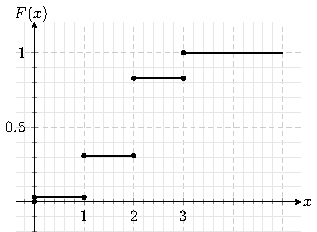
\includegraphics[width=0.5\linewidth]{mai_fig045.pdf}
      \caption{Distribuční funkce k příkladu \ref{mai:exam064}. \cite[s.~233]{Musilova2009MA1}}
      \label{mai:fig045}
    \end{figure}
    Zadáním distribuční funkce je naopak jednoznačně určeno rozdělení veličiny \(X\). Pro jednotlivé
    pravděpodobnosti totiž platí
    \begin{equation*}
      p_j = F(x_j) - F(x_{j-1})\qquad\text{pro}\qquad 2\leq j \leq k, \qquad p_1 = F(x_1).
    \end{equation*}
    
    Hledejme nyní hodnotu \(\overline{x}_P\) definovanou tak, že pravděpodobnost, že při náhodném 
    opakování pokusu nabude veličina \(X\) kterékoli z přípustných hodnot \(x_j \leq 
    \overline{x}_p\), je rovna \(P\). Znamená to, že pro \(x = \overline{x}_P\) má distribuční 
    funkce nabýt předepsané hodnoty \(P\). Abychom \(\overline{x}_P\), takzvaný 
    \(P\)\textbf{-kvantil}, určili, řešíme rovnici
    \begin{equation}\label{mai:eq064}
      \sum_{j=1}^{s}p_j = P
    \end{equation}
    vzhledem k neznámému počtu sčítanců \(s\). V případě veličiny s diskrétním rozdělením se ovšem
    může stát, že pro nevhodně zvolenou hodnotu \(P\) nebude mít rovnice řešení. To proto, že 
    veličina \(X\) může nabývat jen hodnot, které lze očíslovat přirozenými čísly, takže při každé 
    změně horní meze sumy \(s\) o jedničku se suma mění skokem. Vidíme to jak v předcházející 
    tabulce, tak v grafu na obrázku \ref{mai:fig045}. Pro \(P = \num{0.5}\) se \(P\)-kvantil 
    \(\overline{x}_p\), pokud je vůbec definován, nazývá \textbf{medián}. Značí se pouze 
    \(\overline{x}\).

    %--Ještě střelba------------------------------------------------
    % !TeX spellcheck = cs_CZ
\begin{mdframed}[style=mdexam]
  \begin{example}\label{mai:exam067}
    \textbf{Ještě střelba}\newline
    Problém s definici \(P\)-kvantilu u veličiny s diskrétním rozdělením snadno vidíme na příkladu
    střelby (příklad \ref{mai:exam064}). Pro \(s\) postupně 1, 2, 3, 4 nabývá součet na levé straně
    rovnice (\ref{mai:eq064}) hodnot
    
    \begin{equation*}
      p_1 = \num{0.003},\; p_1 + p_2 = \num{0.31},\; p_1 + p_2 + p_3 = \num{0.83}, 
    \end{equation*}
    \begin{equation*}
      p_1 + p_2 + p_3 + p_4 = 1.
    \end{equation*}
    Pojem \(P\)-kvantil je tedy definován jen pro \(P = 0\), \(P = \num{0.03}\), \(P = \num{0.31}\),
    \(P = \num{0.83}\) a \(P = 1\). (Pro \(P = 0\) a \(P = 1\) nemá žádný praktický význam.)
    Nenabývá-li \(P\) žádné z přípustných hodnot, tj. některé hodnoty z množiny \(\{\num{0.03},
    \num{0.31}, \num{0.83}, 1\}\), nemá rovnice pro s řešení a \(P\)-kvantil není vůbec definován.
    Je-li hodnotou \(P\) některý prvek této množiny, dostaneme z rovnice (\ref{mai:eq064}) sice
    jediné řešení \(s\), avšak která hodnota bude \(P\)-kvantilem? Z grafu je vidět, že pro každou
    přípustnou hodnotu \(P\) vyhovuje podmínce celý interval proměnné \(x\). Konkrétní výsledky
    shrnuje následující tabulka:
    
    {\centering
      \begin{tabular}{c|@{\hspace{3pt}}c@{\hspace{3pt}}c@{\hspace{3pt}}c@{\hspace{3pt}}c@{\hspace{3pt}}c}
        \(P\) & \num{0} & \num{0.03} & \num{0.31} & \num{0.83} & \num{1} \\ \hline
        \(F(x) = P\) & \((-\infty,\num{0})\) & \(\left[0, 1\right)\) &
        \(\left[1, 2\right)\) & \(\left[2, 3\right)\) & \(\left[3, \infty\right)\)
      \end{tabular}
    \par}
    
    Význam pojmu \(P\)-kvantil je tedy pro náhodnou veličinu s diskrétním rozdělením poněkud sporný.
    Uplatní se však velmi dobře u veličin s rozdělením spojitým, jak uvidíme později. Než však
    opustíme příklad se střelbou definitivně, spočtěme si ještě střední hodnotu a rozptyl veličiny
    \(X\), kterou jsme definovali jako počet dosažených bodů při jednom výstřelu:
    \begin{align*}
      \langle x \rangle 
          &= \sum_{j=1}^{4}x_jp_j                                                                \\
          &= 0\cdot\num{0.03} + 1\cdot\num{0.28}+ 2\cdot\num{0.52} + 3\cdot\num{0.17} = \num{1.83}, 
    \end{align*}
    \begin{align*}
      D(X)  &= \sum_{j=1}^{4}\left(x_j - \langle x \rangle \right)^2p_j                          \\
            &= (0-\num{1.83})^2\cdot\num{0.03}+(1-\num{1.83})^2\cdot\num{0.28}                   \\
            &+ (2-\num{1.83})^2\cdot\num{0.52}+(3-\num{1.83})^2\cdot\num{0.17}                   \\
                &\simeq\num{0.541},                                                              \\
      \sigma(x) &\simeq\num{0.736}.
    \end{align*}

    V příkladu \ref{mai:exam064} jsme odhadovali, kolika bodů dosáhne střelec při pěti výstřelech.
    Tato hodnota nám vyšla \(\num{5}\cdot\num{1.83} = \num{9.15} = 9\). Nyní vidíme je jí souvislost
    se střední hodnotou náhodné veličiny \(X\). Pokud totiž definujeme veličinu \(Y\) jako počet
    bodů dosažených při pěti výstřelech, je \(Y = 5X\) a \(\langle y \rangle = 5\langle x \rangle\).
    Uvažujme nyní o významu směrodatné odchylky. Zřejmě \(\sigma(y) = 5\sigma(x) = \num{3.68}\).
    Směrodatná odchylka \(\sigma(y)\) určuje interval \((\langle y \rangle - \sigma(y), \langle y
    \rangle + \sigma(y)) = (\num{5.32}, \num{12.68})\). Možnosti bodového zisku ležící v tomto
    intervalu jsou \num{6} až \num{12} bodů včetně. Pokud bychom doplnili tabulku z příkladu
    \ref{mai:exam064} ještě o rozklady a jejich pravděpodobnosti pro bodový součet při pěti
    výstřelech \(j = \num{6}\) a \(j = \num{12}\), dostaneme \(p(A_6) = \num{0.0400}\), \(p(A_{12})
    = \num{0.0550}\). Pravděpodobnost, že výsledek střelce leží při pěti výstřelech v intervalu
    \((\langle y \rangle - \sigma(y), \langle y \rangle + \sigma(y)) = (\num{5.32}, \num{12.68})\),
    je tedy
    \begin{align*}
      \sum_{j=6}^{12}p(A_j) &= p(A_6) + \sum_{j=7}^{11}p(A_j) + p(A_{12})                \\
                            &= \num{0.0400} + \num{0.873} + \num{0.0550} \simeq \num{0.97}.
    \end{align*}
    Při výpočtu jsme využili výsledku z příkladu \ref{mai:exam064}, kde jsme počítali
    pravděpodobnost, že střelec dosáhne bodového výsledku v rozmezí \num{7} až \num{11} bodů.
    Směrodatná odchylka \(\sigma(y)\) veličiny \(Y\) určuje tedy v tomto případě interval okolo
    střední hodnoty \(\langle y \rangle\), v němž leží střelcův bodový zisk s velmi vysokou
    pravděpodobností \SI{97}{\percent}. Tento výsledek lze velmi názorně interpretovat také takto:
    Vystřelí-li střelec pětkrát na terč, bude téměř s jistotou jeho bodový zisk ležet v intervalu
    určeném směrodatnou odchylkou, tj. bude ležet mezi šesti a dvanácti body. Není vyloučeno, že
    bodový zisk bude třeba pět bodů, nebo i nula, nebo naopak dokonce maximálních možných patnáct
    bodů. Všechny ty to možnosti dohromady jsou však vysoce nepravděpodobné, připadá na ně
    pravděpodobnost pouhé \SI{3}{\percent}!. Anebo ještě trochu jinak: Kdyby střelec při tréninku
    uskutečnil třeba sto sérií po pěti výstřelech, pak by skoro jistě bylo sedmadevadesát z nich v
    rozmezí bodového zisku \num{6} až \num{12} bodů a tři mimo. Toto konstatování ovšem opět
    nevylučuje možnost, že v rozmezí \num{6} až \num{12} bodů bude ležet jiný počet sérií než
    \num{97}. Může dokonce v principu dojít k tomu, že do této kategorie padnou série všechny nebo
    žádná. Takový výsledek je však opět vysoce nepravděpodobný.
    
    Není vyloučeno, že i po prostudování tohoto příkladu bude někdo stále nespokojen s tím, že je
    naše vyjadřování „málo přesné“. Vzhledem k pravděpodobnostnímu charakteru posuzovaných jevů
    však, bohužel, přesnější být nemůže.
  \end{example}
\end{mdframed}
    %---------------------------------------------------------------
    
    Příklad \ref{mai:exam067} názorně vypovídá o významu směrodatné odchylky. Viděli jsme, že 
    intervalu o šířce \(2\sigma(y)\) s hodnotou \(\langle y \rangle\) uprostřed odpovídá vysoká 
    pravděpodobnost, že v něm bude ležet bodový zisk střelce při každé pětici výstřelů. Čím bude 
    tento interval užší, tím v průměru blíže budou jednotlivé hodnoty bodového zisku ležet v 
    blízkosti střední hodnoty. Mohli bychom říci, že střelec, jehož výsledky vykazují malou 
    směrodatnou odchylku resp. malý rozptyl, míří přesněji. Směrodatná odchylka je tedy v jistém 
    smyslu jedním z parametrů charakterizujících kvalitu střelby - střelba s malou hodnotou  
    \(\sigma(y)\) je přesnější než střelba s velkou hodnotou \(\sigma(y)\). Druhým parametrem 
    kvality střelby, který je pro její hodnocení z hlediska možnosti vyhrávat soutěže jistě 
    podstatně důležitější, je samozřejmě samotná střední hodnota bodového zisku. Čím je větší, tím 
    je střelcovo pořadí při závodech lepší. Pro interpretaci směrodatné odchylky to ovšem není 
    podstatné. Kdybychom porovnávali dva střelce, jejichž střední bodový zisk při
    pěti výstřelech je třeba \num{12} bodů a \num{3} body, avšak směrodatná odchylka je u obou 
    stejná, musíme konstatovat, že oba jsou stejně přesní. Jeden z nich však systematicky dělá 
    nějakou chybu a přesně střílí do nesprávného místa. Význam pojmu přesnost z hlediska hodnocení 
    náhodných veličin je tedy oproti jeho běžnému chápání poněkud posunut.
    
    Všimněme si ještě jedné důležité obecné věci: Tvar vzorce pro výpočet rozptylu resp. směrodatné 
    odchylky je stejný pro všechny typy rozdělení. Konkrétní pravděpodobnost, že hodnota
    veličiny padne do intervalu určeného směrodatnou odchylkou, tj. do intervalu \((\langle y 
    \rangle - \sigma(y), \langle y \rangle + \sigma(y))\), však pochopitelně na konkrétním 
    rozdělení závisí.

    %--Poissonovo rozdělení-----------------------------------------
    % !TeX spellcheck = cs_CZ
\wikitextrule
\begin{example}\label{mai:exam068}
  \textbf{Poissonovo rozdělení}\newline\small
  Limitním případem Bernoulliova (binomického) rozdělení pro velké hodnoty \(n\), tj. \(n 
  \rightarrow \infty\), a pro \(j \ll n\) je \textbf{rozdělení Poissonovo}. Odvodíme je. Pro velká 
  \(n\) a \(j \ll n\) platí přibližný vzorec
  \begin{equation*}
    n! \simeq n^j(n-j)!,
  \end{equation*}
  a tedy
  \begin{equation*}
    P_j \simeq \lim\limits_{n\rightarrow\infty}\dfrac{n^j}{j!}p^j(1-p)^{n - j}
        \simeq \lim\limits_{n\rightarrow\infty}\dfrac{(np)^j}{j!}\left(1-\dfrac{np}{n}\right)^{n}.
  \end{equation*}
  Při vzpomínce na kapitolu o počítání i limitami a na \textbf{l’Hospitalovo pravidlo} snadno 
  provedeme následující výpočet. O testujte své předchozí znalosti a jednotlivé kroky výpočtu 
  proveďte:
  \begin{equation*}
    \lim\limits_{n\rightarrow\infty}\left(1 - \dfrac{A}{n}\right)^n = 
    \lim\limits_{x\rightarrow0}\left(1 - Ax\right)^\dfrac{1}{x} =
    \exp\left(\lim\limits_{x\rightarrow0}\dfrac{\ln(1 - Ax)}{x}\right) = e^{-A}.
  \end{equation*}
  V našem případě je \(A = np = \langle x \rangle\) (střední hodnota veličiny \(X\) při 
  Bernoulliově rozdělení), takže
  \begin{equation}\label{mai:eq065}
    p_j = \langle x \rangle^j\dfrac{e^{-\langle x \rangle}}{j!}.
  \end{equation}
  Možnost použití Bernoulliova rozdělení si již představit dokážeme. Přinejmenším jsou hody mincemi 
  a kostkami pěkné hříčky. K čemu však je dobré rozdělení Poissonovo? Ja k může vypadat praktická 
  situace, kdy provádíme obrovské množství opakování pokusu a zajímá nás pravděpodobnost pouze 
  malého počtu zdarů? Typickým příkladem takové situace je registrace částic vznikajících při 
  radioaktivním rozpadu. Taková měření jsou potřebná nejen ve fyzikálním výzkumu, ale i v 
  aplikovaných oborech, například v lékařství. Počet \(n\) radioaktivních rozpadů za jednotku času, 
  například za sekundu, je u běžných zdrojů obrovský, zatímco počet těch z nich, které jsou 
  zachycovány detektorem, může být při určitých experimentech malý. Částice se registrují
  pomocí Geigerova-Mullerova počítače, kterým je ionizační komora pracující ve vhodném režimu. 
  Pokud je počet částic \(j\) dopadajících za jednu sekundu do detektoru velmi malý, vyvolá každá z 
  nich měřitelný a dokonce slyšitelný pulz (v obvodu to „praská“). Po registraci částice potřebuje 
  detektor jistou \textbf{mrtvou dobu}, aby se vrátil do výchozího stavu, v němž je schopen 
  registrovat další částici. Tato doba se pohybuje kolem \SI{e-4}{s}. Aby byly jednotlivé pulzy 
  dobře odlišeny, je však třeba, aby do detektoru dopadlo za jednu sekundu mnohem a mnohem méně 
  částic, než jak by odpovídalo převrácené hodnotě mrtvé doby. Zejména pokud bychom chtěli pulzy 
  počítat sluchem, nemělo by jich být více než zhruba jeden až dva každou sekundu. Uvažujme o 
  radioaktivním rozpadu jader cesia \ce{Cs^137}. Jedná se o takzvaný \textbf{beta-rozpad}, který 
  probíhá následovně:
  \begin{itemize}
    \item \ce{Cs^137} \(\longrightarrow\) \ce{Ba^137} + elektron + neutrino, asi \SI{8}{\percent} 
          všech rozpadů
    \item \ce{Cs^137} \(\longrightarrow\) \ce{Ba^137}* + elektron + neutrino, asi \SI{92}{\percent} 
          všech rozpadů
  \end{itemize}
  Excitované baryum \ce{Ba^137}* (jádro má vyšší energii než atom \ce{Ba^137} v základním stavu 
  asi o \SI{0.66}{\mega\electronvolt}  - odpovídá energii \SI{1.1e-13}{\joule}) se pak dále rozpadá 
  podle vzorce
  \begin{itemize}
    \item \ce{Ba137}* \(\longrightarrow\) \ce{Ba137} + částice gama.
  \end{itemize}

  Ze všech částic, které při reakci vznikají, se v Geigerově-Můllerově detektoru registrují 
  elektrony a částice gama, nelze je však od sebe odlišit. Uvažujme o cesiovém zdroji s běžnou 
  hodnotou aktivity, například \SI{10}{\pico\coulomb} (mikrocurie). Jednotka aktivity 
  radioaktivních preparátů \num{1} curie představuje situaci, kdy se za jednu sekundu rozpadá 
  \num{3.7e10} jader. Počet rozpadů, které v průměru nastanou třeba za deset sekund v našem vzorku, 
  je \(n = \num{3700000}\). V Bernoulliově pokusu to odpovídá počtu jeho opakování \(n\). Ja k jsme 
  již řekli, je to obrovský počet. Nastavíme-li experiment tak, abychom registrovali každou sekundu 
  zhruba jednu částici (uslyšíme jeden „prásk“ ), bude počet zdarů \(j\) v Bernoulliově pokusu 
  velmi malý ve srovnání s \(n\). Jsou tedy splněny podmínky pro použití Poissonova rozdělení. 
  Zvolíme například desetisekundový interval měření a počítáme pulzy. Počet registrovaných pulzů 
  \(j\) v tomto intervalu je roven počtu zdarů. Takové měření provedeme třeba dvěstěkrát.
  Označme počet intervalů, v nichž jsme naměřili právě \(j\) pulzů, jako \(\nu(j)\). Celkem je v 
  \(\nu(1) + \cdots + \nu(j_{max}) = \num{200}\). Získáme tak tabulku nebo graf, z nichž pak lze 
  usuzovat na parametry Poissonova rozdělení:
  \begin{table}[ht!]
    \centering
    \resizebox{0.8\textwidth}{!}{%
    \begin{tabular}{c|crrrrrrrrrrrrrrrrr}
      \(j\)      & 0 & 1 & 2 & 3 & 4 & 5 & 6 & 7 & 8 & 9 & 10 & 11& 12& 13 & 14 & 15 & 16 & 17   \\
      \hline
      \(\nu(j)\) & 0 & 4 & 10 & 19 & 28 & 33 & 34 & 26 & 19 & 10 & 6 & 3 & 2 & 2 & 2 & 0 & 1 & 1 \\
    \end{tabular}}
    % \caption{ }
  \end{table}
  Budeme-li předpokládat, že větší počet pulzů v desetisekundovém intervalu je již velmi málo 
  pravděpodobný, můžeme četnosti \(\nu(j)\) považovat za úměrné pravděpodobnostem \(p_j\) 
  Poissonova rozdělení. Všimněme si formule pro Poissonovo rozdělení podrobněji. Je vidět, že platí
  \begin{equation*}
    \dfrac{\nu(j + 1)}{\nu(j)} = \dfrac{p_{j+1}}{p{j}} = \dfrac{\langle x \rangle}{j + 1},
    \qquad p_0 = e^{-\langle x \rangle}.
  \end{equation*}
  Pro hodnotu \(j\), pro kterou jsou si četnosti \(\nu(j)\) a \(\nu(j + 1)\) „nejblíže“, je 
  \(\langle x \rangle \simeq j + 1\). Z tabulky vidíme, že v případě našeho experimentu je 
  \(\langle x \rangle = 6\). Hodnota \(p_0 = e^{-6} \simeq \num{0.002}\) je tedy tak malá, že se 
  ani nedivíme, že jsme mezi dvěma stovkami měření nezaznamenali ani jeden případ, kdy v 
  desetisekundovém intervalu nebyla zaregistrována žádná částice.
  
  Můžeme ještě určit podíly sousedních hodnot \(\nu(j + 1)\) a \(\nu(j)\) a zjistit, zda výsledky 
  našeho experimentu odpovídají vlastnostem Poissonova rozdělení:
  \begin{table}[ht!]
    \centering
    \resizebox{0.7\textwidth}{!}{%
    \begin{tabular}{c|crrrrrrrr}
      \(j\)               & 0 & 1 & 2  & 3  & 4  & 5  & 6  & 7 & 8    \\ \hline
      \(\nu(j+1)/\nu(j)\) & - & \num{2.50} & \num{1.90} & \num{1.47} & \num{1.18} 
                          & \num{1.03} & \num{0.76} & \num{0.73} & \num{0.53}   \\
      \(\langle x \rangle / j + 1\) & \num{6.00} & \num{3.00} & \num{2.00} & \num{1.50} & \num{1.20}
                          & \num{1.00} & \num{0.86} & \num{0.75} & \num{0.67}
    \end{tabular}}
    % \caption{ }
  \end{table}
  \begin{table}[ht!]
    \centering
    \resizebox{0.7\textwidth}{!}{%
    \begin{tabular}{c|crrrrrrrr}
      \(j\)               & 9 & 10 & 11  & 12  & 13  & 14  & 15  & 16 & 17    \\ \hline
      \(\nu(j+1)/\nu(j)\) & \num{0.60} & \num{0.50} & \num{0.67} & - & - & - & - & - & -   \\
      \(\langle x \rangle / j + 1\) & \num{0.60} & \num{0.55} & \num{0.50} & \num{0.46}
                          & \num{0.43} & \num{0.40} & \num{0.38} & \num{0.35} & \num{0.33}
    \end{tabular}}
    % \caption{ }
  \end{table}
  Vidíme, že hodnoty podílů sousedních četností celkem dobře odpovídají vlastnostem Poissonova 
  rozdělení pro \(0 \leq j \leq 12\). Pro \(j > 12\) jsou již četnosti \(\nu(j)\) tak malé, že 
  vytvářet jejich podíly nemá smysl. Tato skutečnost je v tabulce vyznačena pomlčkou.
  
  Poissonovým rozdělením se řídí také například četnost červených krvinek, které se v daném časovém 
  intervalu objeví ve vymezené části zorného pole mikroskopu, četnost zmetků v dodávce zboží, 
  četnost překlepů písařky, apod.  
\normalsize
\end{example}
    %---------------------------------------------------------------
    
    \subsection{Kolik rychlostí má molekula plynu - spojité rozdělení}
      Již nadpis napovídá, že veličina se spojitým rozdělením může zřejmě nabývat „spojitě 
      rozložených“ hodnot, tj. přípustným i hodnotami budou například právě všechna čísla \(x\) z 
      jistého intervalu, \(x\in[a, b]\). Jaká však bude pravděpodobnost \(p(x)\), že veličina \(X\) 
      nabývá právě hodnoty \(x\in[a, b]\)? Jestliže víme, že „součet“ všech \(p(x)\) musí být roven 
      jedné, vzniká problém.
      
      Hodnot \(x\) je totiž nekonečně (dokonce nespočetně) mnoho! Je jich tolik, jako je čísel na 
      celé reálné ose. A kdyby byla pravděpodobnost \(p(x)\) jakkoli malinkatá, nikdy nebude součet 
      všech \(p(x)\) konečný. Pravděpodobnost nabývání hodnoty \(x\) tedy musí být nulová. Vzniklou 
      překážku odstraníme snadno. Rozdělení náhodné veličiny \(X\) bude nutno charakterizovat 
      nikoli pravděpodobností, ale \textbf{hustotou pravděpodobnosti}. Je to obdobná situace jako 
      třeba při popisu rozložení hmotnosti nějakého tělesa, předpokládáme-li, že je ta to hmotnost 
      rozložena v objemu tělesa spojitě. Také nemá příliš smysl se ptát, jaká je hmotnost jednoho 
      bodu tohoto tělesa. I zde by byla odpověď, že nulová. Spíše si vždy klademe otázku, jaká je 
      hmotnost \(\Delta m(\vec{r})\) jistého malého objemu \(\Delta V\), například malého kvádříku, 
      umístěného třeba jedním z vrcholů v bodě o poloze \(\vec{r}\). Hustota \(\varrho(\vec{r})\) 
      tělesa v bodě \(\vec{r}\) je pak limitou podílu \(\Delta m(\vec{r})/\Delta V\) pro \(\Delta V 
      \longrightarrow 0\). Obdobně je tomu i s rozdělením spojité náhodné veličiny \(X\). 
      Zvolíme-li pro jistou hodnotu \(x\) interval \([a, x + \Delta x]\), má smysl otázka, jaké je 
      pravděpodobnost \(\Delta p(x)\), že veličina nabývá hodnoty (kterékoli) právě z tohoto 
      intervalu.

      \adjustbox{minipage=[c]{\textwidth}}{%
        Limitu
        \begin{equation}\label{mai:eq066}
          w(x) = \lim\limits_{\Delta\longrightarrow0}\dfrac{\Delta p(x)}{\Delta x}
        \end{equation}
        nazýváme \textbf{hustotou pravděpodobnosti} veličiny \(X\) v bodě \(x\) (pro \(x = a\), 
        resp. \(x = b\) se jedná o limitu zprava, resp. zleva).
      }
      
      Přímo tato funkce pak představuje ono spojité rozdělení náhodné veličiny \(X\). Určuje totiž
      hustotu pravděpodobnosti \(w\) pro hodnotu \(x\) náhodné veličiny \(X\), obdobně jako \(p_j\) 
      v případě diskrétního rozdělení určuje pravděpodobnost hodnoty \(x_j\). Předpokládejme, že je 
      funkce \(w(x)\) na intervalu \([a, b]\) spojitá.
  
      \adjustbox{minipage=[c]{\textwidth}}{%
        Pro \(x \in [a, b]\) definuje integrál jako funkce horní meze
        \begin{equation}\label{mai:eq067}
          F(x) = \int_a^xw(u)\dd{u}
        \end{equation}
        \textbf{distribuční funkci}.
      }
      Jeho hodnota pro dané \(x\) udává pravděpodobnost, že hodnota veličiny \(X\) padne do 
      intervalu \([a, x]\), opět v plné analogii s případem diskrétního rozdělení. Na \((a, b)\) je 
      tedy hustota pravděpodobnosti \(w(x)\) derivací distribuční funkce. Je zřejmé, že \(F(b) = 
      1\). Integrál z hustoty pravděpodobnosti v mezích \([a, b]\) udává totiž pravděpodobnost, že 
      hodnota veličiny \(X\) padne do intervalu přípustných hodnot, tedy pravděpodobnost jistého 
      jevu. V případě diskrétního rozdělení jsme však distribuční funkci definovali nejen pro 
      přípustné hodnoty náhodné veličiny, ale pro všechna x \in (-\infty, +\infty). Tento postup 
      budeme respektovat i nyní a definujeme
      \begin{equation*}
        F(x) = 0\text{ pro }x \in (-\infty,a)\text{ a }F(x) = 1\text{ pro }x \in (b , +\infty).
      \end{equation*}
      \adjustbox{minipage=[c]{\textwidth}}{%
        \begin{equation}\label{mai:eq068}
          \langle x \rangle = \int_a^bxw(x)\dd{x}, \qquad 
                       D(X) = \int_{a}^{b}(x - \langle x \rangle)^2w(x)\dd{x}.
        \end{equation}
      }
      \textbf{Relativní směrodatná odchylka} je opět podílem \(\sqrt{D(X)}/\langle x \rangle\), 
      nejpravděpodobnější hodnota neboli \textbf{modus} \(x_m\) je taková hodnota veličiny \(X\) , 
      pro kterou je hustota pravděpodobnosti maximální
      
      Daleko lépe než u veličin s diskrétním rozdělením vypadá možnost definovat \(P\)-kvantil 
      \(\tilde{x}_p\) a \textbf{medián} \(\tilde{x}\). Jsou jednoduše řešením rovnic
      \begin{equation*}
        F(\tilde{x}_P) = P, \qquad F(\tilde{x}) = \dfrac{1}{2}
      \end{equation*}
      (Mohli bychom mediánu třeba i říkat „půlkvantil“. To ale není zvykem.) \(P\)-kvantil je 
      definován pro jakoukoli hodnotu \(P\) zadanou v intervalu \((0, 1)\). Skutečně, hustota 
      pravděpodobnosti je nezápornou funkcí na intervalu \([a, b]\) (podle předpokladu i spojitou), 
      takže distribuční funkce je na \([a, b]\) \emph{spojitá} a \emph{rostoucí} a nabývá hodnot 
      \(0 = F(a) \leq F(x) \leq F(b) = 1\). Podle jedné z vět o spojitých funkcích (odstavec 
      2.1.7*) nabývá funkce spojitá na uzavřeném intervalu všech hodnot mezi svým minimem a 
      maximem. V intervalu \([a, b]\) tedy existuje alespoň jedna hodnota \(\tilde{x}_P\) , pro 
      kterou je \(F(\tilde{x}_P) = P\). Ze skutečnosti, že je \(F(x)\) navíc rostoucí, vyplývá, že 
      i \(\tilde{x}_P\) existuje jednoznačně.
  
      Tyto závěry zůstanou v platnosti, i kdyby veličina \(X\) nabývala svých hodnot v intervalu
      typu \(\left[0, \infty\right), \left(—\infty, b\right]\) nebo \((—\infty, \infty)\). Vzhledem 
      k požadavku
      \begin{equation*}
        \int_{a}^{b}w(x)\dd{x} = 1,
      \end{equation*}
      kde kterákoli z mezí \(a\), resp. \(b\) může být i nevlastní, je zřejmé, že funkce \(w(x)\) 
      musí být na svém definičním oboru \(D_f\) omezená. Navíc je na něm spojitá. Vybereme-li tedy 
      jakýkoli uzavřený podinterval oboru \(D_f\), můžeme předchozí argumentaci týkající se 
      \(P\)-kvantilu bez problémů použít.

      %--Normální rozdělení-------------------------------------------
      % !TeX spellcheck = cs_CZ
\begin{mdframed}[style=mdexam]
\begin{example}\label{mai:exam069} \textbf{Normální rozdělení}\\
  Veličinou s normálním rozdělením rozumíme takovou náhodnou veličinu \(X\), jejíž hustota 
  pravděpodobnosti má tvar
  \begin{mdframed}[style=highlight]
    \begin{equation}\label{mai:eq069}
      w(x) = \dfrac{1}{\sigma\sqrt{2\pi}}\exp\left[-\dfrac{(x-\mu)^2}{2\sigma^2}\right],
             \qquad x\in(-\infty, \infty).
    \end{equation}
  \end{mdframed}
  Grafem této funkce je \textbf{Gaussova křivka}. Distribuční funkce má tvar
  \begin{mdframed}[style=highlight]
    \begin{equation}\label{mai:eq70}
      F(x) = \int_{-\infty}^{x}\dfrac{1}{\sigma\sqrt{2\pi}}
               \exp\left[-\dfrac{(t-\mu)^2}{2\sigma^2}\right]\dd{t}.
    \end{equation}
  \end{mdframed}
  udává pravděpodobnost, že hodnota náhodné proměnné je menší než zadaná hodnota (nerovnost může 
  být i neostrá). Přitom \(F(\infty) = 1\) (pravděpodobnost jistého jevu). Skutečně, platí
  \begin{equation*}
    \begin{multlined}
      \int_{-\infty}^{\infty}\dfrac{1}{\sigma\sqrt{2\pi}}
      \exp\left[-\dfrac{(t-\mu)^2}{2\sigma^2}\right]\dd{t}   \\
      \shoveleft[1cm]= \dfrac{\sigma\sqrt{2}}{\sigma\sqrt{2\pi}}
              \int_{-\infty}^{\infty}\exp\left(-u^2\right)\dd{u} =1.
    \end{multlined}
  \end{equation*}
  Takzvaný Laplaceův integrál \(\int_{-\infty}^{\infty}\exp(-u^2)\dd{u} = \sqrt{\pi}\) 
  sice můžeme najít v tabulkách a v dalším dílu jej i odvodíme, v tu to chvíli se však budeme řídit 
  výrokem lorda Kelvina: „Matematik je ten, komu je toto zřejmé jako je zřejmé vám, že dvakrát dvě 
  jsou čtyři.“ Příklady normálního rozdělení pro různé hodnoty \(\sigma,\,\mu\) a odpovídající 
  distribuční funkce vidíme na obrázku \ref{mai:fig046a} a \ref{mai:fig046b}.

  {\centering
    \captionsetup{type=figure}
     \subcaptionbox{\label{mai:fig046a}}{\luafigure[1]{mai_fig046a.pdf}}              \\
     \subcaptionbox{\label{mai:fig046b}}{\luafigure[1]{mai_fig046b.pdf}}
     \captionof{figure}{Hustota pravděpodobnosti normálních rozdělení a jejich distribuční funkce 
              s různými charakteristikami \(\sigma\) a \(\mu\). Červenou čárou je vyznačeno 
              normované normální rozdělení. \cite[s.~240]{Musilova2009MA1}
    \label{mai:fig046}}
  \par}
  \vspace*{10px} Určíme střední hodnotu a rozptyl veličin s tímto rozdělením:
  \begin{align*}
    \langle x \rangle 
      &= \int_{-\infty}^{x}\dfrac{1}{\sigma\sqrt{2\pi}}x\cdot
         \exp\left[-\dfrac{(x-\mu)^2}{2\sigma^2}\right]\dd{x}                                     \\
      &= \dfrac{\sigma\sqrt{2}}{\sigma\sqrt{2\pi}}
         \int_{-\infty}^{\infty}\left(\mu+t\sigma\sqrt{2}\right)\cdot\exp\left(-t^2\right)\dd{t}  \\
      &= \dfrac{\mu}{\sqrt{\pi}}\int_{-\infty}^{\infty}\exp\left(-t^2\right)\dd{t}                \\
      &+ \dfrac{1}{\sqrt{\pi}}\int_{-\infty}^{\infty}t\sigma\sqrt{2}\cdot\exp\left(-t^2\right)\dd{t}
       =\mu.
  \end{align*}
  Druhý z integrálů je totiž roven nule, neboť integrand je lichá funkce.
  \begin{align*}
    D(X)  &= \dfrac{1}{\sigma\sqrt{2\pi}}\int_{-\infty}^{\infty}\left(x - \mu\right)^2 
             \exp\left[-\dfrac{(x-\mu)^2}{2\sigma^2}\right]\dd{x}                                \\
          &= \dfrac{2\sqrt{2}\sigma^3}{\sigma\sqrt{2\pi}}
             \int_{-\infty}^{\infty}t^2\exp\left(-t^2\right)\dd{t}
           = \sigma^2.
  \end{align*}
  Integrál \(\int_{-\infty}^{\infty}t^2\exp\left(-t^2\right)\dd{t} = \frac{\sqrt{\pi}}{2}\) lze buď 
  opět najít v tabulkách, nebo jej metodou per partes převést na výpočet Laplaceova integrálu:
  \begin{align*}
    I &= \int_{-\infty}^{\infty}t\cdot t\exp\left(-t^2\right)\dd{t}         \\
      &= \left[-\dfrac{t}{2}\exp\left(-t^2\right)\right]_{-\infty}^{\infty}
       + \dfrac{1}{2}\int_{-\infty}^{\infty}\exp\left(-t^2\right)\dd{t}.
  \end{align*}
  
  Distribuční funkce normálního rozdělení, zvaná \(errorfunkce\), je běžnou součástí různých 
  počítačových programů, takže poměrně snadno zjistíme pravděpodobnostní obsah intervalu určeného 
  směrodatnou odchylkou \(\sigma(x) = \sqrt{d(X)} = \sigma\). Pravděpodobnost, že hodnota náhodné 
  veličiny \(X\) s normálním rozdělením leží v intervalu \((\mu - \sigma, \mu + \sigma)\), je 
  zhruba \SI{68.3}{\percent}. V souvislosti s normálním rozdělením se často užívají další 
  dva druhy odchylek. \textbf{Pravděpodobná chyba} \(\theta\) určuje interval \((\mu - \theta, \mu 
  + \theta)\), v  němž leží hodnota veličiny \(X\) s pravděpodobností \SI{50}{\percent}. 
  \textbf{Krajní chyba} \(\kappa\) určuje interval \((\mu - \kappa, \mu + \kappa)\), v němž leží 
  hodnota veličiny \(X\) s pravděpodobností \SI{99.7}{\percent}. Z tabelovaných hodnot 
  \(errorfunkce\) zjistíme, že platí
  \begin{equation}\label{mai:eq71}
   \theta \simeq \dfrac{2}{3}\sigma, \qquad \kappa = 3\sigma
  \end{equation}
  Poznamenejme, že normálním rozdělením \(w(x)\) (\ref{mai:eq069}) lze přibližně nahradit 
  Bernoulliovo rozdělení
  \begin{align*}
    w_{Ber}(x)        &= \binom{n}{x}p^x(1 - p)^{n-x},  \\
    \langle x \rangle &= np, \;  D(x) = np(1-p)
  \end{align*}
  pro velké hodnoty \(n\) a také Poissonovo rozdělení
  \begin{equation*}
    w_{Pois}(x) = e^{-\langle x \rangle}\dfrac{\langle x \rangle^x}{x!}, \qquad 
    D(x) = \langle x \rangle
  \end{equation*}
  s velkou střední hodnotou \(\langle x \rangle\)
\end{example}
\end{mdframed}
      %---------------------------------------------------------------
  
      %--Kolik rychlostí má molekula plynu----------------------------
      % !TeX spellcheck = cs_CZ
\wikitextrule
\begin{example}\label{mai:exam070}
  \textbf{Kolik rychlostí má molekula plynu}\newline\small
  Tato otázka se zdá na první pohled zcela nesmyslná. Každý student fyziky ví, že molekuly plynu 
  lze popisovat jako klasické částice, jejichž mechanický stav je jednoznačně určen polohovým 
  vektorem a vektorem rychlosti. Molekula má tedy vždy určitou hodnotu rychlosti. Představte si ale 
  takový plyn ve skutečnosti. Jeden mol jeho látkového množství (např. pro kyslík to představuje 
  hmotnost \num{32} gramů) obsahuje asi \num{6.623e23} molekul! Kdybychom chtěli plyn popisovat 
  jako soustavu klasických částic v mechanice, museli bychom v daném okamžiku znát polohu a 
  rychlost každé molekuly z tohoto obrovského počtu. A to je principiálně nemožné, protože do 
  chování takové soustavy zasahuje velmi podstatným způsobem „náhoda“. Nemůžeme určit, ve kterém
  bodě prostoru právě daná molekula je a jak rychle se pohybuje. Dokážeme pouze určit, s jakou 
  pravděpodobností se nachází v elementárním objemu \(\Delta V = \Delta x \Delta y \Delta z\) v 
  okolí daného bodu o polohovém vektoru \(\vec{r}\) a s jakou pravděpodobností \(\Delta P\) leží 
  koncový bod vektoru její rychlosti v elementárním objemu \(\Delta\Omega = \Delta v_x \Delta v_y 
  \Delta v_z\) „rychlostního“ prostoru v okolí zadané rychlosti \(\vec{v}\). Uvažujme o 
  nejjednodušším modelu plynového tělesa, takzvaném ideálním plynu, jehož molekuly jsou stejné a 
  navzájem neinteragují s výjimkou kratičkých náhodných srážek. Molekuly takového plynu jsou z 
  hlediska pravděpodobnostního popisu navzájem ekvivalentní. Pravděpodobnost \(\Delta P\) bude pro 
  všechny stejná a pro velmi malé elementární objemy bude dána vztahem
  \begin{equation*}
    \Delta P(\vec{r},\vec{v}) = \varrho(\vec{r},\vec{v})\Delta V \Delta\Omega,
  \end{equation*}
  kde \(\varrho(\vec{r},\vec{v}) = \varrho(x, y, z, v_x, v_y, v_z)\) je odpovídající hustota 
  pravděpodobnosti. Jak ale hustota konkrétně závisí na polohách a rychlostech molekul? Tento 
  fyzikální zákon, zvaný \textbf{Gibbsovo rozdělení}, se řídí exponenciální funkcí
  \begin{equation*}
    \varrho(\vec{r},\vec{v}) = K\exp\left(-\dfrac{E(\vec{r},\vec{v})}{kT}\right)
  \end{equation*}
  kde \(E\) je \textbf{mechanická energie molekuly} (kinetická plus potenciální v případném silovém 
  poli), \(T\) je \textbf{absolutní teplota plynu} udávaná v kelvinech a \(k = 
  \SI{1.38e-23}{\joule\per\kelvin}\) je \textbf{Boltzmannova konstanta}.
  
  Zajímá-li vás, proč si příroda v tomto případě vybrala zrovna exponenciální funkci, sledujte 
  následující orientační úvahu: Rozdělme si v myšlenkách plynové těleso na dvě části, jimž 
  odpovídají energie \(E_1\) a \(E_2\). Celková energie soustavy je \(E = E_1 + E_2\). Označme 
  \(P(E)\) pravděpodobnost, že, se soustava nachází ve stavu s energií \(E\), pravděpodobnosti, že 
  se jednotlivé části nachází nezávisle ve stavech s energiemi \(E_1\) a \(E_2\), pak jako
  \(P(E_1)\) a \(P(E_2)\). Pravděpodobnost, že se první část soustavy nachází ve stavu s energií 
  \(E_1\) a \textbf{současně} druhá část ve stavu s energií \(E_2\), je rovna součinu 
  pravděpodobností těchto nezávislých jevů. Proto \(P(E_1 + E_2) = P(E_1) \cdot P(E_2)\). Tuto 
  vlastnost mají ovšem právě exponenciální funkce. Platí tedy \(\varrho \approx\exp(\beta E)\). 
  Konstantu \(\beta\) určí jen experiment, z něhož vychází \(\beta = - (kT)^{-1}\).
  
  Vrátíme se nyní k výchozímu problému, neboť úvodní otázka nabyla smyslu: Molekula může mít 
  libovolnou rychlost s větší či menší pravděpodobností. Nebude-li ideální plyn umístěn v žádném 
  silovém poli, bude mechanická energie molekuly dána pouze energií kinetickou. Elementární 
  pravděpodobnost, že koncový bod rychlosti molekuly leží v elementárním objemu \(\Delta\Omega\) v 
  okolí bodu \(\vec{v}\) „rychlostního“ prostoru, bez ohledu na to, v jaké části „obyčejného“, tj. 
  \textbf{konfiguračního prostoru} se vyskytuje, je
  \begin{equation*}
    \Delta P(\vec{v}) = \varrho(\vec{v})\Delta\Omega 
                      = C\exp\left(-\dfrac{m(v_x^2 + v_y^2 + v_z^2)}{2kT}\right)\Delta\Omega.
  \end{equation*}
  Tato pravděpodobnost, jak je vidět, nezávisí na směru rychlosti, pouze na její velikosti, 
  \(\varrho(\vec{v}) = \varrho(v)\). Konstantu \(C\) určíme snadno. Pravděpodobnost, že molekula má 
  vůbec nějakou rychlost, je rovna jedné (jistý jev). Matematický zápis této skutečnosti vyžaduje 
  znalost takzvaného trojného integrálu (integrujeme podle tří proměnných  - složek vektoru 
  rychlosti). V našem případě se však výpočet redukuje na součin tří integrálů jednoduchých,
  \begin{equation*}
    \int_{\Omega}\varrho(v_x, v_y, v_z)\dd{v_x}\dd{v_y}\dd{v_z} = 1
  \end{equation*}
  \begin{equation*}
    \Rightarrow C \cdot
     \int_{-\infty}^{\infty}\exp\left(\dfrac{mv_x^2}{2kT}\right)\dd{v_x} \cdot
     \int_{-\infty}^{\infty}\exp\left(\dfrac{mv_y^2}{2kT}\right)\dd{v_y} \cdot
     \int_{-\infty}^{\infty}\exp\left(\dfrac{mv_z^2}{2kT}\right)\dd{v_z} =1.
  \end{equation*}
  Po substitucích \(mv_i^2/2kT = u^2,\, i = x, y, z\) vede výpočet na \textbf{Laplaceův integrál}
  \begin{equation*}
    \int_{-\infty}^{\infty}\exp(-u^2)\dd{u} = \sqrt{\pi}.
  \end{equation*}
  Dostáváme
  \begin{equation*}
    C = \left(\dfrac{m}{2\pi kT}\right)^{\frac{3}{2}} \Rightarrow
    \Delta P(\vec{v}) = \left(\dfrac{m}{2\pi kT}\right)^{\frac{3}{2}}
                        \exp\left(- \dfrac{mv^2}{2 kT}\right)\dd{v_x}\dd{v_y}\dd{v_z}
  \end{equation*}
  Hustota pravděpodobnosti je stejná pro všechny koncové body vektoru rychlosti \(\vec{v}\) ležící 
  v rychlostním prostoru na kulové ploše o poloměru rovném velikosti rychlosti \(v\). Jaká bude 
  elementární pravděpodobnost \(\Delta P(v)\), že molekula má velikost rychlosti v intervalu \((v, 
  v + \Delta v)\) bez ohledu na směr pohybu? Tuto pravděpodobnost dostaneme, vezmeme-li za 
  \(\Delta\Omega\) objem tenké kulové slupky o poloměru \(v\) a tloušťce \(\Delta v\), v níž končí 
  všechny vektory rychlosti, jejichž velikost leží v požadovaném intervalu. Tento objem je 
  \(\Delta\Omega = 4\pi v^2\Delta v\) a
  \begin{equation*}
    P(v) = 4\pi\left(\dfrac{m}{2\pi kT}\right)^{\frac{3}{2}}v^2
               \exp\left(- \dfrac{mv^2}{2 kT}\right)\Delta v = f_M(v)\Delta v. 
  \end{equation*}

  {\centering
   \captionsetup{type=figure}
   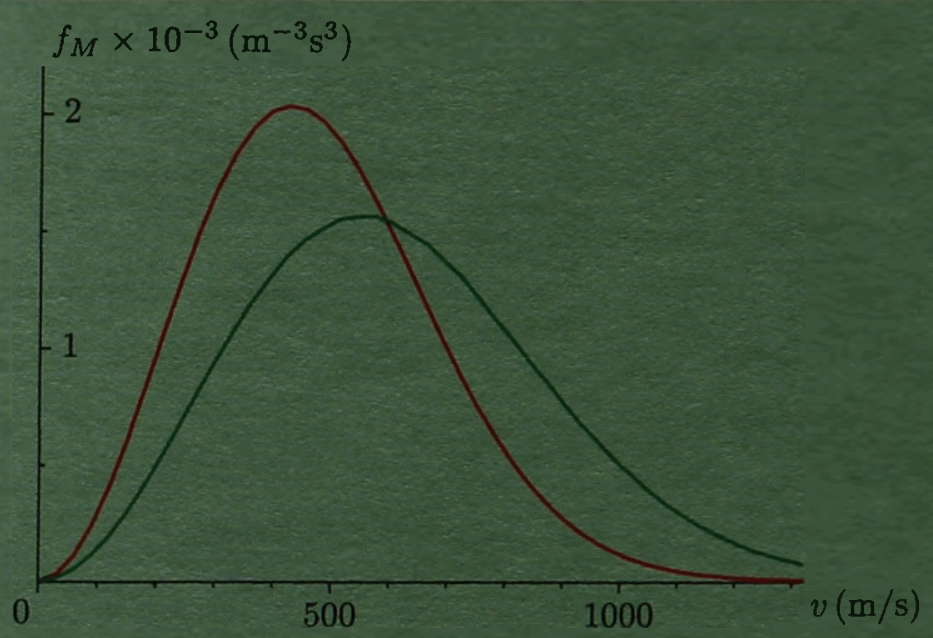
\includegraphics[width=0.4\linewidth]{mai_fig048.png}
   \captionof{figure}{Maxwellovo rozdělení rychlostí molekul dusíku pro teploty \(T_1 = 
                      \SI{300}{\kelvin}\) a \(T_2 = \SI{300}{\kelvin}\).
   \cite[s.~243]{Musilova2009MA1}
   \label{mai:fig048}}
  \par}
  
  Dokážete vyložit, proč jsme zvolili za \(\Delta\Omega\) celý objem slupky? Počítáme totiž 
  pravděpodobnost, že koncový bod vektoru rychlosti molekuly leží, zhruba řečeno, v kterémkoli 
  elementárním kvádříku \(\Delta v_x\Delta v_z\Delta v_z\) obsaženém ve slupce. A ta je součtem 
  pravděpodobností odpovídajících všem kvádříkům vytvářejícím slupku. Jedná se o pravděpodobnosti 
  navzájem neslučitelných jevů (pohybuje-li se molekula v jednom směru, nepohybuje se v jiném). 
  Hustota této pravděpodobnosti se nazývá \textbf{Maxwellovo rozdělení rychlostí}. Na rozdíl od 
  Gaussova rozdělení, popisujícího hustotu pravděpodobnosti pro jednotlivé složky rychlosti, je 
  nesymetrická vlivem faktoru \(v^2\). Obrázek \ref{mai:fig048} ukazuje funkci \(f_M(v)\) pro dvě 
  různé teploty \(T_2 > T_1\). Důležité hodnoty spjaté s tímto rozdělením jsou 
  \textbf{nejpravděpodobnější rychlost} \(v_p\), \textbf{střední rychlost} \(\langle v \rangle\) a 
  \textbf{střední kvadratická rychlost} \(\langle v^2 \rangle\). Platí
  \begin{align*}
    \der{f_M}{v}        &= 0\, \longrightarrow v_P = \sqrt{\dfrac{2kT}{m}},                      \\
    \langle v \rangle   &= \int_{-\infty}^{\infty}vf_M(v)\dd{v} = \sqrt{\dfrac{8kT}{\pi m}},     \\
    \langle v \rangle^2 &= \int_{-\infty}^{\infty}v^2f_M(v)\dd{v} = \dfrac{3kT}{m}.
  \end{align*}
\normalsize
\end{example}
      %---------------------------------------------------------------
  
  \section{Náhoda a zpracování měření}\label{mai:IchapIIIsecIV}
    \subsection{Součet a součin náhodných veličin}
      Nyní vyřešíme ještě jeden důležitý problém. Víme již, že veličinu \(Y = f(X)\) lze popsat 
      stejnými pravděpodobnostmi jako veličinu \(X\). V řadě případů je však náhodná veličina \(Y\) 
      funkcí několika náhodných veličin \(X_1, X_2, \ldots, X_s\). Každá z nich má nějaké 
      rozdělení. Jaké potom bude rozdělení veličiny \(Y\)? Rozebereme jen dvě základní situace, z 
      nichž je ovšem možné „poskládat“ řadu případů složitějších. Půjde o situace, kdy náhodná 
      veličina bude součtem nebo součinem dvou náhodných veličin, pro jednoduchost značení 
      například \(U\) a \(V\), tedy \(Y = U + V\), \(Z = U \cdot V\). Předpokládejme nejprve, že 
      veličiny \(U\) a \(V\) jsou zcela nezávislé, tj. hodnoty veličiny \(U\) nejsou nijak 
      ovlivněny hodnotami veličiny \(V\) a naopak. Dejme tomu, že \(U\) a \(V\) mají rozdělení
      \begin{equation*}
        \left\lbrace (u_1, p_1), \ldots, (u_k, p_k) \right\rbrace, \qquad
        \left\lbrace (v_1, q_1), \ldots, (v_\ell, v_\ell) \right\rbrace
      \end{equation*}
      Veličiny \(Y = U + V\), resp. \(Z = U \cdot V\) tedy mohou nabývat hodnot \(\lbrace u_i + 
      v_\alpha\rbrace\), resp. \(\lbrace u_i v_\alpha\rbrace\) s pravděpodobnostmi \(p_iq_\alpha\). 
      Jevy \uv{Veličina \(U\) nabude hodnoty \(u_i\)} a \uv{veličina \(V\) nabude hodnoty 
      \(v_\alpha\)} jsou totiž nezávislé. Rozdělení veličin \(Y\) a \(Z\) je 
      \begin{equation*}
        \lbrace (u_i +v_\alpha, p_iq_\alpha)\rbrace,\, \text{resp.}\,
        \lbrace(u_iv_\alpha, p_iq_\alpha)\rbrace,\qquad 1\leq i\leq k,\quad 1\leq\alpha\leq\ell,
      \end{equation*}
      Pro jejich střední hodnoty dostáváme
      \begin{align*}
        \langle y \rangle 
          &= \sum_{i=1}^{k}\sum_{\alpha=1}^{\ell}(u_i + v_\alpha)p_iq_\alpha
           = \sum_{i=1}^{k}u_ip_i\left(\sum_{\alpha=1}^{\ell}q_\alpha\right) + 
             \sum_{\alpha=1}^{\ell}v_\alpha q_\alpha\left(\sum_{i=1}^{k}p_i\right)  \\
          &= \sum_{i=1}^{k}u_ip_i + \sum_{\alpha=1}^{\ell}v_\alpha q_\alpha         \\
        \langle z \rangle 
          &= \sum_{i=1}^{k}\sum_{\alpha=1}^{\ell}(u_i \cdot v_\alpha)p_iq_\alpha
           = \left(\sum_{i=1}^{k}u_ip_i\right)
             \left(\sum_{\alpha=1}^{\ell}v_\alpha q_\alpha\right) 
           = \langle u \rangle \langle v \rangle.
      \end{align*}
      Střední hodnota součtu, resp. součinu náhodných veličin je tedy součtem, resp. součinem jejich
      středních hodnot. Pro součet náhodných veličin platí tento výsledek i v případě, když nebudou
      nezávislé. V tak jednoduchý závěr jsme snad ani nedoufali! Hned uvidíme, jak jej lze využít.
      
      %--Jak číst výsledky studentské ankety aneb není průměr jako průměr----------
      % !TeX spellcheck = cs_CZ
\wikitextrule
\begin{example}\label{mai:exam071}
  \textbf{Jak číst výsledky studentské ankety aneb není průměr jako průměr}\newline\small
  Každý semestr na Masarykově univerzitě se uzavírá vyhodnocením velmi užitečné studentské ankety v 
  Informačním systému MU. Studenti hodnotí na jedenáctihodnotové stupnici (nula až deset bodů) 
  několik položek pro každý studijní předmět (obtížnost, zajímavost, srozumitelnost výkladu, 
  přístup učitele, rozmanitost literatury) a mohou doplnit i slovní komentáře. Na ty se učitelé 
  těší nejvíce, neboť díky anonymitě pisatelů se tak o sobě mohou dovědět leccos zajímavého. 
  Všimneme si však statistického zpracování ankety. U každého předmětu je pro danou položku 
  vypočtena průměrná bodová hodnota odpovědí a vyznačena na téže jedenáctihodnotové stupnici. Pro 
  porovnání je na stupnici vyznačen i takzvaný „fakultní průměr“. Každý přednášející může vidět svá 
  hodnocení a hodnocení svých kolegů, kteří mu vedou cvičení. Děkan má přístupové právo k celé
  statistice, a tak může porovnávat. Jednoho deštivého večera přestalo děkana bavit vyplňování 
  rektorátních formulářů a začal si výsledky ankety prohlížet. Zajímala jej zejména položka 
  „srozumitelnost výkladu“. Řekl si, že všem učitelům, kteří v této položce budou hodnoceni 
  nadprůměrně, zvýší osobní ohodnocení. Soubor předmětů je veliký, a tak děkan klikal a klikal. 
  Zjišťoval, že u veliké většiny předmětů leží průměrné hodnocení srozumitelnosti nad fakultním 
  průměrem. Jeho pocity byly smíšené. Na jedné straně se radoval, jakými jsou jeho podřízení 
  dobrými pedagogy, na druhé straně trnul, kolik to bude stát. Snad aby se raději vrátil 
  k protivným formulářům. Najednou v něm zahlodalo podezření i naděje, že není všechno v pořádku. 
  Jak je možné, že většina hodnocení leží nad průměrem? Kladné a záporné odchylky by se přece měly 
  kompenzovat. Zavolal proto na koberec proděkana pro informační technologie, aby se jej zeptal, co 
  je to „fakultní průměr“. Proděkan odpověděl takto: Máme soubor \(K\) předmětů \(\lbrace 
  X_\alpha\rbrace\), \(\alpha = 1, \ldots, K\). V předmětu \(X_\alpha\) vyplnilo anketu 
  \(N_\alpha\)  studentů, jednotlivé hodnoty odpovědí pro danou položku (srozumitelnost výkladu) 
  byly označeny \(\lbrace x_{\alpha,j}\rbrace\), \(j = 1, \ldots, N_\alpha\). Celkem přirozeně 
  předpokládáme, že váha odpovědi každého studenta je stejná, nezávisle na předmětu. Tato váha je
  rovna převrácené hodnotě celkového počtu studentů, kteří vyplnili anketu, tj. \(w = N^{-1}\), \(N 
  = N_1 + \ldots + N_k\). Fakultní průměr je proto dán vzorcem
  \begin{equation*}
    \langle x \rangle 
      = \sum_{\alpha=1}^{K}\sum_{j=1}^{N_\alpha}wx_{\alpha,j} 
      = \dfrac{1}{N}\sum_{\alpha=1}^{K}\left(\sum_{j=1}^{N_\alpha}x_{\alpha,j}\right)
      = \dfrac{1}{N}\sum_{\alpha=1}^{K}A_\alpha,
  \end{equation*}
  kde jsme označili \(A_\alpha = \sum_{j=1}^{N_\alpha}x_{\alpha,j}\). Děkan chvíli přemýšlel a 
  pravil: To vypadá docela logicky. Neměli bychom však počítat fakultní průměr tak, že vezmeme 
  průměrné hodnoty pro každý předmět a vypočteme jejich aritmetický průměr? Pak bychom dostali
  \begin{equation*}
    \langle \overline{x} \rangle
      = \dfrac{1}{K}\sum_{\alpha=1}^{K}\langle x_{\alpha}\rangle
      = \dfrac{1}{K}\sum_{\alpha=1}^{K}
        \left(\dfrac{1}{N_\alpha}\sum_{j=1}^{N_\alpha}x_{\alpha,j}\right)
      = \dfrac{1}{K}\sum_{\alpha=1}^{K}\dfrac{A_\alpha}{N_\alpha}.
  \end{equation*}
  Tento závěr se akademickým funkcionářům na první pohled nijak zvlášť nelíbil. Bylo totiž jasné, 
  že náhodné veličiny \(X_1, \ldots, X_k\) mají odlišná rozdělení. No jo, řekli si oba, musíme 
  počítat. My už ale počítat nemusíme, neboť jsme takový problém před chvílí vyřešili obecně. 
  Zjistili jsme totiž, že střední hodnota součtu náhodných veličin je rovna součtu středních 
  hodnot, bez ohledu na konkrétní rozdělení každé z veličin. Definujeme-li tedy náhodnou veličinu 
  \(Y\) jako aritmetický průměr veličin \(X_\alpha\), tj.
  \begin{align*}
    Y &= \dfrac{1}{K}\left(X_1 + \ldots + X_K\right),  \\
    \shortintertext{dostaneme}
    \langle y \rangle &= \dfrac{1}{K}\left(\langle x_1 \rangle +\ldots+\langle x_K \rangle\right).
  \end{align*}
  Tento výsledek se shoduje s hodnotou \(\langle \overline{x} \rangle\), kterou pro výpočet 
  „fakultního průměru“ navrhl děkan. Vypočteme-li součet odchylek hodnot \(\langle x_\beta 
  \rangle\) od \(\langle y \rangle\), dostaneme skutečně nulu:
  \begin{equation*}
    \sum_{\beta =1}^{K}\left(\langle x_\beta \rangle - \langle y \rangle\right)
      = \sum_{\beta =1}^{K}\left(\dfrac{A_\beta}{N_\beta} 
      - \dfrac{1}{K}\sum_{\alpha=1}^{K}\langle x_\alpha \rangle\right)
      = 0.
  \end{equation*}
  Zkusme se ještě zamyslet nad tím , jak použití „špatného“ fakultního průměru zkreslilo výsledky a 
  proč. Vypočtěme si rozdíl \(\Delta = \langle \overline{x} \rangle - \langle x \rangle\):
  \begin{equation*}
    \Delta = \langle \overline{x} \rangle - \langle x \rangle 
      = \dfrac{1}{K}\sum_{\alpha=1}^{K}\langle x_\alpha \rangle
      - \dfrac{1}{N}\sum_{\alpha=1}^{K}A_\alpha
      = \dfrac{1}{K}\sum_{\alpha=1}^{K}\langle x_\alpha \rangle
      - \dfrac{1}{N}\sum_{\alpha=1}^{K}N_\alpha\langle x_\alpha \rangle
      = \dfrac{1}{K}\sum_{\alpha=1}^{K}\langle x_\alpha\rangle\left(1 - K\dfrac{N_\alpha}{N}\right).
  \end{equation*}
  Platí přitom
  \begin{equation*}
    \sum_{\alpha=1}^{K}\left(1 - K\dfrac{N_\alpha}{N}\right) = 0.
  \end{equation*}
  Pokud by byl počet studentů, kteří vyplnili anketu, ve všech předmětech stejný, tj. \(N_\alpha = 
  \dfrac{N}{K}\) , byla by odchylka \(\Delta\) podle očekávání nulová. Stejná situace by nastala, 
  kdyby byly shodné všechny průměrné hodnoty \(\langle x_\alpha \rangle\). Je-li odchylka 
  \(\Delta\) kladná, je „nesprávný“ fakultní průměr \(\langle x \rangle\) nižší než \(\langle 
  \overline{x} \rangle\). Proto hodnocení jednotlivých předmětů vypadají příznivěji, právě tak, jak 
  to zjistil děkan. Odchylku \(\Delta\) posouvají do kladných hodnot předměty, které hodnotilo málo 
  studentů, a předměty, které měly vysoké hodnocení. Dobře je to vidět na příkladu dvou předmětů, 
  tj. pro \(K = 2\), kde vychází
  \begin{equation*}
    \Delta = \langle \overline{x} \rangle - \langle x \rangle 
           = \dfrac{N_2 - N_1}{2(N_2+N_1)}\left(\langle\overline{x}\rangle-\langle x\rangle\right).
  \end{equation*}
  
  Pro \(N_1\ll N_2\) a \(\langle x_1 \rangle  \gg \langle x_2 \rangle \) bude rozdíl \(\Delta\) 
  skoro polovina hodnoty \(\langle x_1 \rangle\)! U volitelných specializovaných předmětů, které si 
  vybírají jen poměrně malé počty studentů, kteří navíc mají o předmět opravdový zájem a hodnotí 
  jej proto většinou vyšším počtem bodů, je splněno obojí (malý počet hodnotících a vysoké bodové
  hodnocení). Je vidět, že při nesprávně zvoleném výpočtu srovnávací hodnoty (fakultního průměru) 
  mohou právě předměty, jejichž statistický význam je spíše okrajový, ovlivnit celkové hodnocení.
\normalsize
\end{example}
      %----------------------------------------------------------------------------
      
      Pro střední hodnotu součtu a součinu nezávislých náhodných veličin jsme získali velmi
      jednoduché výsledky:
      
      \adjustbox{minipage=[c]{\textwidth}}{%
        \begin{equation}\label{mai:eq070}
          \langle u + v \rangle = \langle u \rangle + \langle v \rangle\qquad
          \langle uv \rangle    = \langle u \rangle \langle v \rangle.
        \end{equation}
      }
      
      Dokážeme také určit rozptyl veličin \(Y = U + V\) a \(Z = U\cdot V\)? Pro rozptyl každé 
      náhodné veličiny platí obecný vztah (\ref{mai:eq061}). Použijeme jej pro naše konkrétní 
      případy:
      \begin{align*}
        D(U + V) &= \langle (u + v)^2 \rangle - \langle u + v \rangle^2 
                  = \langle u^2 + 2uv + v^2 \rangle - \left(\langle u \rangle^2 +
                    \langle 2uv \rangle + \langle v^2 \rangle\right)                        \\
                 &= \left(\langle u^2\rangle - \langle u \rangle^2\right)
                  + \left(\langle v^2\rangle - \langle v \rangle^2\right) = D(U) + D(V).
      \end{align*}
      Pro rozptyl náhodné veličiny \(Z = U \cdot V\) dostaneme
      \begin{align*}
        D(Z)  &= \langle z^2\rangle - \langle z \rangle^2 
               = \langle u^2\rangle\langle v^2\rangle - \langle u \rangle^2 \langle v \rangle^2  \\
              &= \left[D(U) + \langle u^2\rangle\right]\left[D(V) + \langle v^2\rangle\right]
               - \langle u \rangle^2 \langle v \rangle^2                                         \\
              &= D(U)D(V) + \langle u \rangle^2D(V) + \langle v \rangle^2D(U).
      \end{align*}
      Pak
      \adjustbox{minipage=[c]{\textwidth}}{%
        \begin{equation*}
          \dfrac{D(z)}{ \langle z \rangle^2} = \dfrac{D(U)}{ \langle u \rangle^2} \cdot
            \dfrac{D(V)}{ \langle v \rangle^2} + \dfrac{D(U)}{ \langle u \rangle^2} +
            \dfrac{D(v)}{ \langle v \rangle^2}.
        \end{equation*}
      }
      Při výpočtu jsme využili vztahu (\ref{mai:eq061}) a vztahů (\ref{mai:eq070}) pro střední 
      hodnotu součtu a součinu náhodných veličin. Pokud mají veličiny \(U\) a \(V\) shodný rozptyl 
      \(D(U) = D(V) = D\), pak je \(D(U + V) = 2D\). V případě součtu s veličin \(Y = X_1 + \cdots 
      + X_s\) se shodným rozptylem \(D\) resp. směrodatnou odchylkou \(\sigma\) dostáváme
      \begin{equation*}
        D(Y) = sD  \Rightarrow \sigma(y) = \sqrt{s}\sigma.
      \end{equation*}
      Znovu připomeňme, že všechny vztahy týkající se součtu a součinu náhodných veličin, které
      jsme zatím získali, platí za předpokladu, že výchozí veličiny, které sčítáme nebo násobíme, 
      jsou nezávislé.
      
      Aniž bychom se podrobněji zabývali vlastnostmi rozdělení závislých veličin, definujeme pro
      ně charakteristiky, které tuto závislost popisují. Nechť \(U\) a \(V\) jsou dvě libovolně 
      náhodné veličiny, ne nutně nezávislé. Míru jejich závislosti určují veličiny
      \begin{equation}\label{mai:eq071}
        \sigma_{uv} = \langle (u - \langle u \rangle) (v - \langle v \rangle) \rangle, \qquad
        \varrho_ {uv}=\dfrac{\sigma(u)}{\sqrt{D(U)D(V)}} = \dfrac{\sigma(u)}{\sigma{D(u)\sigma(v)}}
      \end{equation}
      zvané \textbf{kovariance} a \textbf{korelační koeficient} veličin \(U\) a \(V\). Platí 
      \(\varrho(uv) \leq 1\). Pro nezávislé veličiny vychází \(\sigma(uv) = 0\) a \(\varrho(uv) = 
      0\).
      
      %-- Rozptyl při Bernoulliově pokusu-----------------------------
      % !TeX spellcheck = cs_CZ
\begin{mdframed}[style=mdexam]
  \begin{example}\label{mai:exam072}
    \textbf{Rozptyl při Bernoulliově pokusu}\newline
    V příkladu \ref{mai:exam066} jsme se zajímali o střední hodnotu veličiny \(X\) definované jako
    počet zdarů při \(n\) opakováních Bernoulliova pokusu. Řekli jsme si, že střední hodnota této
    veličiny je \(np\) s tím, že důkaz lze provést přímo na základě definičního vztahu pro střední
    hodnotu matematickou indukcí. Výpočet rozptylu z definičního vztahu bychom jistě snadno dokázali
    zahájit, horší by však bylo dovést jej do konce. Stačí se podívat na začátek výpočtu
    \begin{align*}
      D(X) &= \sum_{j=0}^n \left(x_j - \langle x \rangle\right)^2p_j             \\
           &= \sum_{j=0}^n \left(j - np\right)^2\binom{n}{j}p^j(1 - p)^j,
    \end{align*}
    a nepochybujeme o tom, že tuto sumu nedokážeme spočítat snadno. Protože již však umíme zacházet
    se součtem náhodných veličin, můžeme využít účinného triku. Veličinu \(X\) si představíme jako
    součet
    \begin{equation*}
      X = U_1 + U_2 + \cdots + U_n,
    \end{equation*}
    kde každá z veličin \(U_j\) může nabývat dvou hodnot. Jedničky v případě, že při \(j\)-tém
    opakování pokusu nastal zdar, a nuly v případě, že nastal nezdar. Součet všech veličin \(U_j\)
    pro \(j = 1\) až \(j = n\) pak skutečně znamená celkový počet zdarů při \(n\) opakováních
    pokusu. Jestliže si uvědomíme, že pravděpodobnost zdaru při kterémkoli z opakování je \(p\) a
    pravděpodobnost nezdaru \((1 - p)\), ihned vidíme, že rozdělení každé z veličin \(U_j\) má tvar
    \(\lbrace(1, p), (0, 1 - p)\rbrace\). Platí tedy
    \begin{equation*}
      \langle u_j\rangle = 1\cdot p + 0 \cdot (1 - p) = p,
    \end{equation*}
    \begin{align*}
      D = D(U_j) &= \left( 1 - \langle u_j\rangle\right)^2p 
                  + \left( 0 - \langle u_j\rangle\right)^2(1 - p)   \\
                 &= p(1 - p)^2 + p^2(1 - p) = p(1 - p).
    \end{align*}
    Každé dvě veličiny \(U_i\), \(U_j\) jsou nezávislé, neboť jednotlivá opakování pokusu jsou
    nezávislá. Střední hodnota jejich součtu je: tedy \(np\) (a to souhlasí s informací v příkladu
    \ref{mai:exam066}) a pro rozptyl jejich součtu platí
    \begin{equation*}
      D(X) = nD = np(1 - p).
    \end{equation*}
    Celkově tedy dostáváme
    \begin{equation*}
      \langle x \rangle = np, \; \sigma(x) = \sqrt{np(1 - p)}.
    \end{equation*}
  \end{example}
\end{mdframed}
      %---------------------------------------------------------------
      
      %-- Rozptyl aritmetického průměru-------------------------------
      % !TeX spellcheck = cs_CZ
\begin{mdframed}[style=mdexam]
  \begin{example}\label{mai:exam073}
    \textbf{Rozptyl aritmetického průměru}\newline
    Již v úvodu odstavce o náhodných veličinách jsme konstatovali, že opakujeme-li v nezměněných
    podmínkách měření jisté fyzikální veličiny (délka závěsu kyvadla, proud procházející vodičem,
    napětí na vodiči, atd.), budeme díky náhodným vlivům dostávat pokaždé poněkud jiný výsledek.
    Říkáme, že měření je zatíženo náhodnými chybami. Výsledek získaný při každém opakování lze
    interpretovat jako hodnotu náhodné veličiny. Dejme tomu, že jsme provedli uměření fyzikální
    veličiny \(X\) a získali hodnoty \(x_1\) až \(x_n\) . V praktické situaci budou tyto hodnoty
    většinou navzájem různé, nemusí tomu tak však nutně být. Fyzikální veličinu chceme ovšem
    reprezentovat jediným údajem, a tím bude její střední hodnota, tj.
    \textbf{aritmetický průměr}
    \begin{equation*}
      \langle x \rangle = \dfrac{x_1 + x_2 + \cdots + x_n}{n}.
    \end{equation*}
    Rozptyl veličiny \(X\) je dán vztahem
    \begin{align*}
      D &= D(X)                                                             \\
        &= \dfrac{\left(x_1 - \langle x \rangle\right)^2 + 
                  \left(x_2 - \langle x \rangle\right)^2 + \cdots +
                  \left(x_n - \langle x \rangle\right)^2}{n}.
    \end{align*}
    Víme, že směrodatná odchylka \(\sigma( x ) = \sqrt{D(X)}\) určuje, nakolik jsou jednotlivé
    výsledky měření v průměru odchýleny od střední hodnoty, charakterizuje tedy přesnost každého
    opakování měření. Podívejme se na celou úlohu z jiné strany: Představme si, že sledujeme \(n\)
    po dvou nezávislých náhodných veličin \(X_1\) až \(X_n\) se shodnou střední hodnotou \(\langle
    x_j \rangle = \langle x \rangle\) a shodnou směrodatnou odchylkou \(\sigma(x_j) = \sqrt{D},\, 1
    \leq j \leq n\). Aritmetický průměr těchto veličin,
    \begin{equation*}
      \langle \Xi \rangle = \dfrac{X_1 + X_2 + \cdots + X_n}{n}.
    \end{equation*}
    je tedy rovněž náhodnou veličinou. Pro jeho střední hodnotu, rozptyl a směrodatnou odchylku
    platí
    \begin{align*}
      \langle \xi \rangle 
                  &= \dfrac{n\langle x \rangle}{n}, \\
      D(\Xi)      &= \dfrac{1}{n^2}\cdot D(X_1 + \cdots + X_n)=\dfrac{nD^2}{n^2}=\dfrac{D}{n}, \\
      \sigma(\xi) &= \dfrac{\sigma(x)}{\sqrt{n}}.
    \end{align*}
  \end{example}
\end{mdframed}
      %---------------------------------------------------------------
      
      Můžeme tedy říci, že aritmetický průměr všech výsledků měření dané fyzikální veličiny je
      \(\sqrt{n}\)-krát přesnější než jednotlivý výsledek měření. Jakkoli se toto konstatování zdá 
      intuitivně zřejmé, je třeba je používat s opatrností.
      
      Především je třeba mít na mysli, co toto konstatování znamená. Jeho charakter je totiž
      opět jen pravděpodobnostní. Jestliže jsou jednotlivá měření prováděna za stejných podmínek,
      jsou rozdělení veličin \(X_1\) až \(X_n\) funkcemi téhož typu. Tyto veličiny mají také 
      stejnou střední hodnotu \(\langle x \rangle\) a směrodatnou odchylku \(\sigma\). Také 
      pravděpodobnost, že při měření padne hodnota veličiny \(X_j\) do intervalu \((\langle x 
      \rangle - \sigma, \langle x \rangle + \sigma)\), je pro všechna \(j\) prakticky stejná. 
      Označme ji \(P_\sigma\).  Se stejnou pravděpodobností nabude aritmetický průměr \(\Xi\) 
      hodnoty v intervalu určeném svou směrodatnou odchylkou. Ta je však \(\sqrt{n}\)-krát menší. V 
      tomto smyslu jsou hodnoty aritmetického průměru \uv{\(\sqrt{n}\)-krát méně rozptýleny} kolem 
      střední hodnoty \(\langle\xi \rangle\) než hodnoty náhodných veličin \(X_j\) kolem svých 
      středních hodnot \(\langle x \rangle\).
      
      Dalším problémem může být splnění výchozích předpokladů, které vedly ke vztahu pro
      směrodatnou odchylku aritmetického průměru. Ukážeme to na následujícím příkladu.
      
      %-- Jak přesně lze změřit čínského císaře?----------------------
      % !TeX spellcheck = cs_CZ
\wikitextrule
\begin{example}\label{mai:exam075}
  \textbf{Ověření Ohmová zákona}\newline\small

\normalsize
\end{example}
      %---------------------------------------------------------------
      
      %-- Záhada přijímací zkoušky aneb k čemu může posloužit distribuční funkce-----
      % !TeX spellcheck = cs_CZ
\begin{mdframed}[style=mdexam]
  \begin{example}\label{mai:exam075}
    \textbf{Záhada přijímací zkoušky aneb k čemu může posloužit distribuční funkce?}\newline
    Mohlo by se zdát, že distribuční funkce je jen teoretický pojem a že v praktických situacích ji
    těžko využijeme. Podstatné je přece pravděpodobnostní rozdělení náhodné veličiny a distribuční
    funkce je z něj jen jaksi odvozena sčítáním pravděpodobností (u diskrétního rozdělení) nebo
    integrací (u rozdělení spojitého). Přesvědčíme se, že existují velmi realistické případy, kdy
    distribuční funkce přináší věrohodnější informaci o náhodné veličině než samotné rozdělení.
    
    Na Masarykově univerzitě musí každý uchazeč o studium, ať již se hlásí na přírodovědeckou,
    právnickou, lékařskou či jinou fakultu, absolvovat Test studijních předpokladů. Jedná se o
    všeobecný test, zaměřený na zjišťování úrovně všech schopností uchazeče, které jsou potřebné pro
    univerzitní studium, například analytického myšlení, verbálních schopností, numerického myšlení,
    geometrické představivosti, atd. Pro nás však v tu to chvíli není podstatný obsah testu, ale
    způsob zpracování jeho výsledků a vyhodnocení pořadí uchazečů. Test skládá kolem třiceti tisíc
    studentů. Není tedy možné technicky zajistit, aby proběhl v jediné variantě v jednom dni. K
    dispozici je proto osm variant testu, každou variantu řeší tři až čtyři tisíce studentů. Test má
    \num{80} otázek, základním údajem pro zpracování jeho výsledků je počet správných odpovědí
    každého studenta. Pokud bychom označili jako \(i\) počet správných odpovědí (\(i \in\lbrace0, 1,
    2, \ldots, 80\rbrace\)) v kterékoli variantě a \(\mathcal{N}_i\) počet studentů, kteří dosáhli
    právě \(i\) správných odpovědí, dostaneme náhodnou veličinu \(X_i\), kterou bychom mohli nazvat
    „počet správných odpovědí“, pro celou univerzitu. Její rozdělení by mělo tvar
    \begin{equation*}
      \lbrace(i,p_i)\rbrace,\quad\text{kde}\qquad p_i = \dfrac{\mathcal{N}_i}{\mathcal{N}}, \quad
      \mathcal{N} = \sum_{i=0}^{80}\mathcal{N}_i
    \end{equation*}
    A zde je malý „kámen úrazu“. A by bylo možné sestavit opravdu „univerzální pořadí“, musely by
    být všechny varianty testu ekvivalentní z hlediska obtížnosti. To znamená, že kdyby kterýkoli
    student vyplnil za stejných podmínek všechny varianty, dosáhl by v každé z nich stejného počtu
    správných odpovědí s pravděpodobností velmi blízkou jedné. Skutečnost je však principiálně
    taková, že u sebelépe promyšleného a sestaveného testu se jednotlivé varianty budou mírně, v
    rámci statistických, a tedy již neodstranitelných, odchylek lišit. Tato odlišnost se nepozná
    předem, ale až po zpracování výsledků všech variant. Použít pro stanovení pořadí uchazečů
    rozdělení náhodné veličiny \(X\) \emph{= počet správných odpovědí je tedy nespravedlivé}.
    Student, který řešil variantu „statisticky obtížnější“, by v pořadí skončil s horším umístěním,
    než student, který je stejně schopný, avšak měl to štěstí, že na něj připadla varianta
    „statisticky méně obtížná“. Skutečně, kdybychom sestavili grafy rozdělení náhodných veličin
    \(X^{(\alpha)}\) \emph{= počet správných odpovědí v \(\alpha\)-té variantě},
    \begin{equation*}
      \lbrace(i,p_i^{(\alpha)})\rbrace,\quad\text{kde}\; 
      p_i^{(\alpha)} = \dfrac{\mathcal{N}_i^{(\alpha)}}{\mathcal{N}^{(\alpha)}}, \quad
      \mathcal{N}^{(\alpha)} = \sum_{i=0}^{80}\mathcal{N}_i^{(\alpha)}
    \end{equation*}
    zjistili bychom, že se mírně liší. (V předchozím zápisu značí \(\mathcal{N}_i^{(\alpha)}\) počet
    studentů, kteří odpověděli správně na \(i\) otázek \(\alpha\)-té varianty
    \(\mathcal{N}^{(\alpha)}\) je počet všech studentů, kteří tuto variantu řešili.) Střední hodnoty
    i mediány náhodných veličin se i při vynikající shodě obtížnosti všech variant mohou lišit v
    rozmezí jedné až dvou správných odpovědí. A s ohledem na skutečnost, že každou variantu řeší
    obrovský počet studentů, až čtyři tisíce, je zřejmé, že tento rozdíl může poněkud „zamíchat
    “pořadím, zejména v blízkosti mediánu, kde se týká třeba i tří stovek studentů v každé variantě.
    Situaci dokládá obrázek \ref{mai:fig049}. Jak tedy zařídit, abychom dostali spravedlivé pořadí?
    Jediný rozumný způsob, jak minimalizovat vliv statistických odchylek obtížnosti jednotlivých
    variant, je nehodnotit studenty podle absolutního počtu správných odpovědí, ale nějak je
    porovnat mezi sebou. Budeme při tom předpokládat, že rozložení schopností studentů je ve všech
    osmi skupinách, které řeší osm daných variant, stejné. Řeknete si - zase nějaké další
    předpoklady. To je jako z bláta do louže. Předpoklad o stejném rozložení schopností studentů v
    tak velkých skupinách, jako jsou ty naše, je však mnohem realističtější než předpoklad o
    dokonalé shodě obtížnosti variant testu. Budeme se jej proto držet. Každému studentovi
    přisoudíme číslo, které informuje o tom, kolik řešitelů dané varianty bylo horších nebo stejně
    dobrých jako on, tj. mělo nižší nebo stejný počet správných odpovědí. Z matematického hlediska
    to znamená přejít v každé variantě od rozdělení k distribuční funkci. Věnujme se nyní tomuto
    přepočtu podrobněji jak pro diskrétní rozdělení náhodné veličiny \(X^{(\alpha)}\), které
    odpovídá skutečné situaci, tak pro zajímavost i pro rozdělení spojité. V dalším budeme vždy
    zpracovávat výsledky jedné varianty, upustíme proto od vyznačování indexu \(\alpha\).

    {\centering
    \captionsetup{type=figure}
    \luafigure[0.8]{mai_fig049.png}
    \captionof{figure}{Rozdělení pro dvě varianty testu,
    \cite[s.~252]{Musilova2009MA1}
    \label{mai:fig049}}
    \par}
    
    \textbf{Diskrétní rozdělení}
      \begin{itemize}
        \item \emph{Zadání:} Skupina \(N\) studentů řeší jednu variantu testu. Test má \(Q\) otázek.
              Za každou správnou odpověď je přidělen jeden výchozí bod. Získáváme rozdělení
              \begin{gather*}
                \left\lbrace\left(i, \dfrac{N_i}{N} \right)\right\rbrace, \;
                i\in\lbrace0, 1, 2, \ldots, Q\rbrace, \;
                \sum_{i=0}^{Q}N_i = N 
              \end{gather*}
              kde \(i\) je počet výchozích bodů a \(N_i\) počet studentů, kteří získali \(i\) bodů.
              Distribuční funkce tohoto rozdělení
              \begin{gather*}
                F(x) = \dfrac{1}{N}\sum_{i=0}^{j}N_i\;\text{ pro }\;
                j\leq x < j+1, \; x\in\left[0,\infty\right)
              \end{gather*}
              Pro uchazeče, který získal \(j\) bodů, mají význam následující hodnoty:
              \begin{itemize}
                \item \(F(x)    x \in \left[j, j+1\right)\): poměrný počet uchazečů, kteří získali
                      počet výchozích bodů nižší nebo shodný s daným uchazečem,
                \item \(NF(x)   x \in \left[j, j+1\right)\): absolutní počet uchazečů, kteří získali
                      počet výchozích bodů nižší nebo shodný s daným uchazečem,
                \item \(100F(x) x \in \left[j, j+1\right)\): absolutní počet uchazečů, kteří získali
                      počet výchozích bodů nižší nebo shodný s daným uchazečem,
              \end{itemize}
        \item Hodnoty distribuční funkce můžeme získat z následující tabulky:
        
              {\centering
                \resizebox{0.8\textwidth}{!}{%
                \begin{tabular}{c|c}
                          interval \(x\)     &  \(NF(x)\)         \\ \hline
                  \(\left[0,1\right)\)       &  \(N_0\)           \\ 
                  \(\left[1,2\right)\)       &  \(N_0 + N_1\)     \\ 
                  \(\cdots\)                 &  \(\cdots\)        \\
                  \(\left[j,j+1\right)\)     &  \(N_0 + N_1 + \cdots + N_j\) \\ 
                  \(\cdots\)                 &  \(\cdots\) \\
                  \(\left[Q-1,Q\right)\)     &  \(N_0 + N_1 + \cdots + N_{Q-1}\) \\ 
                  \(\left[Q,\infty\right)\)  &  \(N_0 + N_1 + \cdots + N_{Q} = N\) 
                \end{tabular}}
              \par}
        \item Přepočet hodnocení uchazečů tak, aby nová stupnice byla opět v rozsahu mezi nulou a
              \(Q\) a aby nové hodnocení bylo opět celočíselné, je následující:
              \begin{equation*}
                y =QF(x), \quad 0\leq F(x) \leq 1, \Rightarrow y \in[0,Q].
              \end{equation*}
              Uchazeči se ziskem \(i\) výchozích bodů náleží hodnota \(y = QF(x)\) právě když i\(
              \in \left[i, i + 1\right)\), tj. \(y_i = Q F(i)\). Tato hodnota není obecně
              celočíselná. Zaokrouhlení se provede ve prospěch uchazeče, tedy vždy nahoru. Výsledný
              převodní vzorec je
              \begin{equation*}
                \begin{multlined}
                  \text{výchozí body } i \longrightarrow\text{ nové body }  \\ 
                  \shoveleft[1cm]Y_i: Y_i = [y_i] + 1 = [QF(i)] + 1,
                \end{multlined}
              \end{equation*} 
              kde \([a]\) značí celočíselnou část čísla \(a\), tedy například \([\num{23.05}] =
              [\num{23.48}] = [23,89] = 23\)
        \item Zaveďme novou náhodnou veličinu \(Z\) s rozdělením \(\left\lbrace(z_\alpha,
              M_\alpha)\right\rbrace\): Označme \(z_1, z_2, \ldots, z_\alpha, ...,\) \(z_S\)
              navzájem různé hodnoty ze souboru \(\lbrace Y_i\rbrace, i = 0, 1, 2, \ldots, Q\)
              řazené vzestupně. Její rozdělení udává kterákoli z následujících tabulek:

              {\centering
                \resizebox{0.9\textwidth}{!}{%
                \begin{tabular}{c|c}
                          hodnota                       &  četnost         \\
                          \hline
                  \(z_1 = Y_0 = Y_1 = \cdots Y_{i_1}\)  & \(M_1 = N_0 + N_1 + \cdots + N_{i_1}\)  \\ 
                  \(Z_2 = Y_{i_1+1} = \cdots Y_{i_2}\)  & \(M_2 = N_{i_1+1} + \cdots + N_{i_2}\)  \\ 
                  \(\cdots\)                            & \(\cdots\)                              \\
                  \(Z_S = Y_{i_{S-1}+1}=\cdots Y_{i_S}\)& \(M_S = N_{i_{S_1}+1}+\cdots+N_{i_S}\)   
                \end{tabular}}
              \par}

              {\centering
                \resizebox{0.9\textwidth}{!}{%
                \begin{tabular}{c|c}
                          hodnota                        &  četnost         \\
                          \hline
                  \(z_1 = Y_0 = Y_1 = \cdots Y_{i_1}\)   &  \(M_1 = NF(i_1)\)              \\
                  
                  \(Z_2 = Y_{i_1+1} = \cdots Y_{i_2}\)   &  \(M_2 = N[F(i_2) - F(i_1)]\)  \\ 
                  \(\cdots\)                             &  \(\cdots\)                     \\
                  \(Z_S = Y_{i_{S-1}+1}=\cdots Y_{i_S}\) & \(M_S = N[F(i_S) - F(i_{S-1})]\)   
                \end{tabular}}
              \par}
              kde \(i_1 < i_2 < \ldots < i_{S-1} < i_S, i_S = Q\) (Vzhledem k zaokrouhlování nahoru
              není žádná bodová hodnota \(Y_i\) nulová.) I když skutečné rozdělení při zpracování
              výsledků testů je diskrétní, ukažme si, jak by vypadal analogický postup u rozdělení
              spojitého, kde je početní zpracování názornější.
      \end{itemize}
    
    \textbf{Spojité rozdělení}
      \begin{itemize}
        \item \emph{Zadání:} Je dáno rozdělení četností \(n(x) \leq 0,\, x \in [0, Q]\).
        \item Normovací podmínka a distribuční funkce jsou
              \begin{equation*}
                \int_{0}^{Q}n(x)\dd{x} = N, \quad 
                F(x) = \dfrac{1}{n}\int_{0}^{x}n(\xi)\dd{\xi},                
              \end{equation*}
              kde \(0 \leq F(x) \leq 1.\)
        \item Označme \(z = QF(x)\), tedy \(z \in [0, Q]\), novou náhodnou veličinu. (Uvědomme si,
              že \(z\) je rostoucí funkcí proměnné \(x\)). Označme její rozdělení \(\nu(z)\). Její
              distribuční funkce je
              \begin{align*}
                \Phi(z) &= \int_{0}^{z}\nu(\zeta)\dd{\zeta} 
                         = \int_{0}^{x(z)}\dfrac{n(\xi)}{N}\dd{\xi}          \\
                        &= F\left(F^{-1}(z/Q)\right) 
                        = \dfrac{z}{Q}, \quad
                \nu(z) = \dfrac{1}{Q}.
              \end{align*}
        \item Rozdělení je konstantní s mediánem i střední hodnotou \(Q/2\). Takové rozdělení se
              nazývá rovnoměrné.
      \end{itemize}
  \end{example}
\end{mdframed}
      %------------------------------------------------------------------------------
      
    \subsection{Který výsledek je ten pravý?}
      První věc, kterou budete dělat ve fyzikálním praktiku, bude zjišťování průměrné hustoty 
      materiálu, z něhož je vyroben kovový váleček. Budete váleček vážit, abyste určili jeho 
      hmotnost,a měřit jeho výšku a průměr, abyste mohli vypočítat jeho objem. Hustotu stanovíte 
      jako podíl hmotnosti a objemu. Jedná se stále o jeden a týž váleček, jehož průměrná hustota 
      má za daných podmínek (stálá teplota, váleček se nedeformuje, apod.) stále stejnou „správnou“ 
      hodnotu, kterou však neznáme. (Nezná ji ani učitel v praktiku, i když se tak tváří.) Změří-li 
      hustotu válečku všichni studenti ve skupině, každý jen jednou, získá se řada různých hodnot. 
      Která z nich je ta správná? Není vyloučeno, a je to dokonce velmi pravděpodobné, že žádná. A 
      mohli bychom pomocí nich správnou hodnotu určit nebo se k ní alespoň přiblížit? Možné by to 
      bylo, pokud bychom zaručili, že všechny výsledky získané jednotlivými studenty jsou „stejně 
      hodnotné“. Znamenalo by to, že bychom museli vyloučit hrubé a systematické chyby, které by 
      vznikly třeba tak, že by někteří studenti vážili na vadných vahách, někteří by měli špatné 
      měřítko, popřípadě by odečítali údaj „zboku“, takže by byl zkreslený, nebo by se dokonce 
      zmýlili při odečítání údaje. Museli bychom také zaručit, že náhodné vlivy, které ovlivňují 
      měření, zatěžují je náhodnými chybami a v principu je nelze odstranit, byly při všech 
      měřeních stejné. U různých studentů si tím však nemůžeme být jisti (vzpomeňte si na měření 
      čínského císaře), proto budeme raději postupovat tak, že jeden pečlivý student provede větší 
      počet měření třeba výšky válečku, která je pro určení hustoty potřebná. Dejme tomu, že bude 
      měřit milimetrovým měřítkem a bude odhadovat s přesností na půl milimetru. Jeho údaje tedy 
      mohou mít tvar \SI{33.0}{\mm}, \SI{34.5}{\mm}, atd. Získá takto za stejných podmínek třeba 
      dvacet nebo i padesát hodnot, ale co teď s nimi? Jak určit hodnotu, která se bude nejvíce 
      blížit správné hodnotě výšky válečku? (Dalo by se jistě diskutovat i o tom, co je to správná 
      hodnota. Pro tuto chvíli však předpokládejme, že taková hodnota skutečně existuje, neboť 
      váleček je opravdu válcem, je vysoustružen pečlivě, přesněji, než jsme schopni jej měřit, při 
      měření se nemění teplota, váleček není dáván do lisu a deformován, ani upravován tak, že by 
      se měnila jeho hmotnost.) Předpokládejme, že správná hodnota výšky válečku je \(x\) a že 
      student naměřil hodnoty \(\lbrace x_1, X_2, \ldots, x_n\rbrace\), mezi nimiž mohou být 
      pochopitelně i některé hodnoty stejné. Odchylky jeho měření od správné hodnoty jsou
      \begin{equation*}
        \lbrace \varepsilon_1, \varepsilon_2, \ldots, \varepsilon_n\rbrace, \qquad
        \varepsilon_i = x_i - x, \qquad i = 1, 2, \ldots, n.
      \end{equation*}
      I kdybychom správnou hodnotu \(x\) znali, nedokázali bychom předpovědět, nakolik se od ní při
      jednotlivém měření odchýlíme. Můžeme, se však zajímat o to, jaká je pravděpodobnost, že
      hodnota, o kterou bude měření od správné hodnoty odkloněno, bude ležet v určitém intervalu.
      Odchylky \(\varepsilon_i\) lze totiž interpretovat jako hodnoty náhodné veličiny. Abychom 
      mohli požadované pravděpodobnosti určit, potřebujeme znát rozdělení této veličiny. Označme ji 
      \(\varepsilon\) a odpovídající hustotu pravděpodobnosti \(\mathcal{w}(\varepsilon)\). Toto 
      rozdělení je za určitých podmínek \textbf{rozdělením normálním}, splňuje tedy vztah 
      (\ref{mai:eq069}). Zkusme se o tom přesvědčit. Zvolme podmínky měření tak, aby byly ve hře 
      jen náhodné chyby způsobené \(m\) nezávislými vlivy. Každý z nich hodnotu měření
      odchýlí od \(x\) o stejně velkou hodnotu \(\alpha\), kladnou nebo zápornou, s 
      pravděpodobností \num{0.5}. Schéma této úvahy je na obrázku \ref{mai:fig050}. Výsledná 
      odchylka naměřené hodnoty \(x_i\) od hodnoty správné s jistotou leží v intervalu \((-m\alpha, 
      m\alpha)\) a může nabývat pouze hodnot celých násobků \(\alpha\). Při uplatnění jednotlivého 
      „chybového“ vlivu vzniká, jak jsme již řekli, kladná nebo záporná odchylka o velikosti 
      \(\alpha\). Vznik odchylky \(+\alpha\) nazveme zdarem, vznik odchylky \(-\alpha\) nezdarem.
      
      \begin{figure}[ht!] %\ref{mai:fig050}
        \centering
        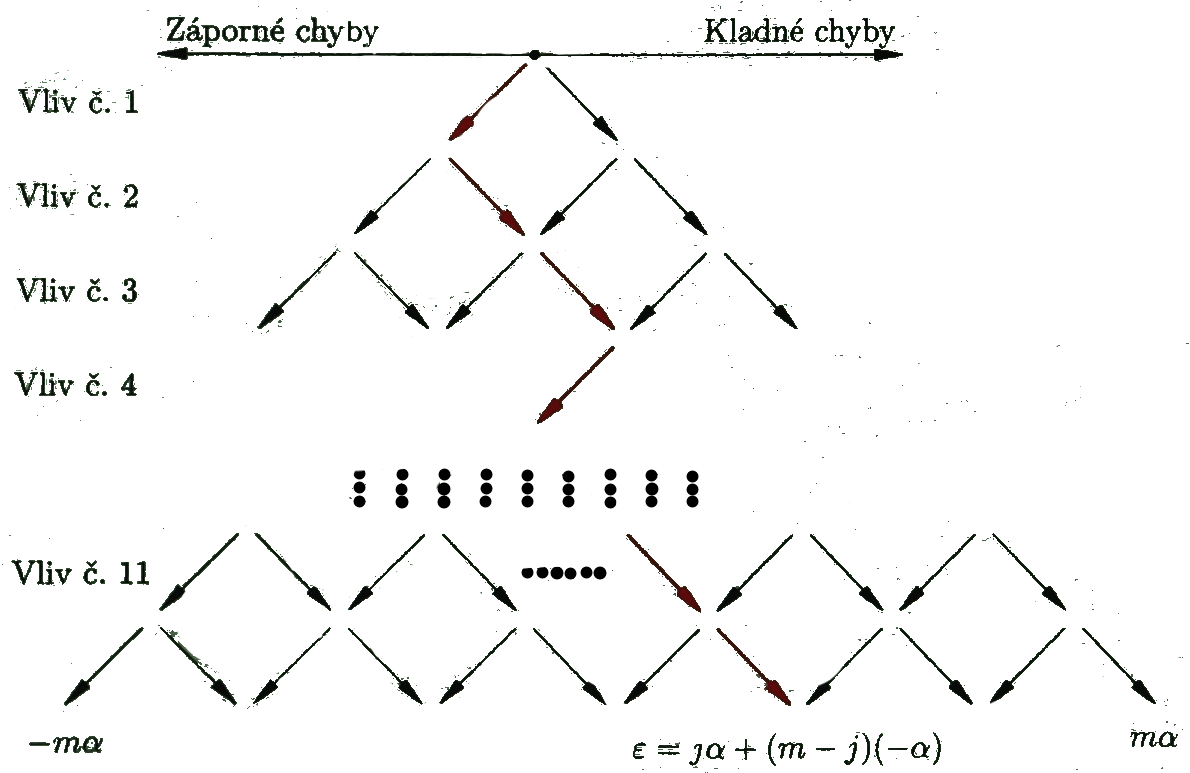
\includegraphics[width=0.6\linewidth]{mai_fig050.png}
        \caption{Vznik kladných a záporných odchylek při měření s \(m\) vlivy. 
        \cite[s.~255]{Musilova2009MA1}}
        \label{mai:fig050}
      \end{figure}
      
      Mohlo by tomu být i naopak, slova „zdar“ a „nezdar“ zde nemají svůj obvyklý význam, jde
      pouze o to, že díky nim můžeme hned uvidět souvislost s Bernoulliovým pokusem a tedy
      i s Bernoulliovým rozdělením. Při \(j\) kladných a \(m — j\) záporných odchylkách je měření od
      správné hodnoty odkloněno o
      \begin{equation*}
        j\alpha + (m - j)(-\alpha) = (2j - m)\alpha
      \end{equation*}
      s pravděpodobností
      \begin{equation*}
        p_j = \begin{pmatrix}m j\end{pmatrix}p^j(1 - p)^{m - j} = 2^{-m}.
      \end{equation*}
      Střední hodnota náhodné veličiny \(\varepsilon\) je nulová. Skutečně, v příkladu 
      \ref{mai:exam066} jsme zjistili, že střední hodnota veličiny \(Y\) nabývající hodnot \(y_j = 
      j\) s Bernoulliovým rozdělením je \(\langle y \rangle = mp\), střední hodnota veličiny \((2j 
      — m)\) a pak musí být \((2mp — m)\alpha\). Pro \(p = \num{0.5}\) je tato hodnota nulová.
      Pro velká \(m\) lze Bernoulliovo rozdělení nahradit rozdělením normálním (obr. 3.8), a proto 
      má náhodná veličina \(\varepsilon\) hustotu pravděpodobnosti tvaru (\ref{mai:eq069}), tj.
      \begin{equation*}
        \mathcal{w}(\varepsilon) = 
        \dfrac{1}{\sigma\sqrt{2\pi}}\exp\left(\dfrac{-\varepsilon^2}{2\sigma^2}\right).   
      \end{equation*}
      \begin{figure}[ht!] %\ref{mai:fig051}
        \centering
        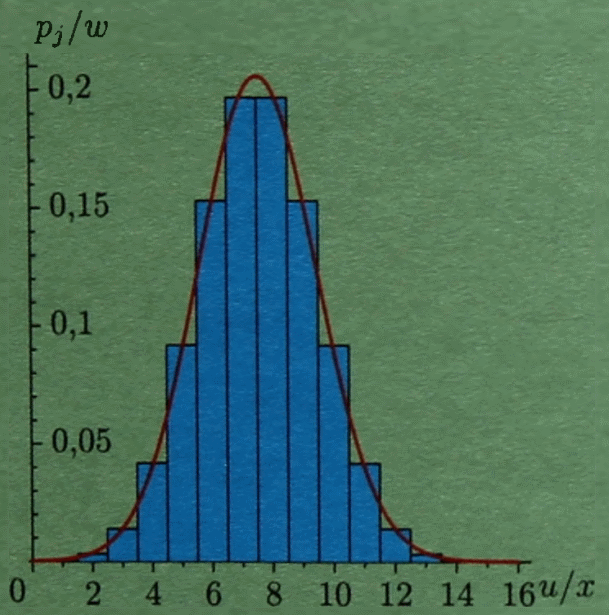
\includegraphics[width=0.4\linewidth]{mai_fig051.png}
        \caption{Normální rozdělení jako limitní případ Bernoulliova 
        \cite[s.~256]{Musilova2009MA1}}
        \label{mai:fig051}
      \end{figure}
      
      Vraťme se nyní k otázce zpracování naměřených hodnot \(\lbrace x_1, \ldots, x_n\rbrace\) 
      výšky válečku. Jejich odchylky od správné hodnoty jsou \(x_1 - x\) až \(x_n - x\). Na místě 
      neznámé správné hodnoty \(x\) si nyní představme nějakou proměnnou, označme ji 
      \(\varepsilon\). Budeme se snažit určit její hodnotu \(\varepsilon_0\) tak, aby 
      pravděpodobnost, že odchylky jednotlivých měřených hodnot od \(\varepsilon_0\) padnou 
      současně do intervalů
      \begin{equation*}
        \left(\varepsilon_1 - \dfrac{\dd{\varepsilon_1}}{2}, 
              \varepsilon_1 + \dfrac{\dd{\varepsilon_1}}{2}
        \right),
        \left(\varepsilon_2 - \dfrac{\dd{\varepsilon_2}}{2}, 
              \varepsilon_2 + \dfrac{\dd{\varepsilon_2}}{2}
        \right), \cdots,
        \left(\varepsilon_n - \dfrac{\dd{\varepsilon_n}}{2}, 
              \varepsilon_n + \dfrac{\dd{\varepsilon_n}}{2}
        \right),
      \end{equation*}
      byla maximální. Pro tuto pravděpodobnost v závislosti na \(\xi\) platí
      \begin{align}
        \dd{W} &= \dd{\mathcal{w}(\varepsilon_1)}\cdots\dd{\mathcal{w}(\varepsilon_n)}  \nonumber\\
               &= \dfrac{1}{\sigma\sqrt{2\pi}}
                  \exp\left(-\dfrac{(x_1 - \xi)^2 + \cdots + (x_n - \xi)^2}{2\sigma^2}
                      \right)\dd{\varepsilon_1}\cdots\dd{\varepsilon_n}.      \label{mai:eq072}
      \end{align}
      (Víte proč je ve vztahu (\ref{mai:eq072}) součin pravděpodobností?) Tato pravděpodobnost bude 
      maximální, bude-li hodnota exponentu minimální. Z podmínky
      \begin{equation*}
        (x_1 - \xi)^2 + \cdots + (x_n - \xi)^2 = \text{min}
      \end{equation*}
      dostáváme derivací podle \(\xi\) požadavek
      \begin{equation*}
        2(x_1 - \xi) + \cdots + 2(x_n - \xi) = 0 \Rightarrow \xi_0 = 
        \dfrac{1}{n}\sum_{i=1}^{n}x_j = \langle x \rangle.
      \end{equation*}
      Vidíme, že veličina, která charakterizuje míru odchýlení naměřených hodnot od \(\xi\), je 
      minimální, zvolíme-li za \(\xi\) aritmetický průměr naměřených hodnot. Pozor, zjištěný 
      výsledek znamená právě jen konstatovanou skutečnost: Při dosazení aritmetického průměru za 
      proměnnou \(\xi\) bude pravděpodobnost, že odchylky jednotlivých měření od \(\xi\) budou 
      ležet v uvažovaných intervalech, maximální. Neznamená to, že správnou hodnotou veličiny \(X\) 
      je aritmetický průměr měření \(x_1, X_2, \ldots, x_n\). Správnou hodnotu ze souboru měření 
      prostě nezjistíme, avšak aritmetický průměr je jí blízký s vysokou pravděpodobností. Jaká je 
      tato „blízkost“ a její pravděpodobnost konkrétně? Hned uvidíme. Správnou hodnotu výšky 
      válečku \(x\) sice neznáme, ale víme, že náhodná veličina \(\varepsilon\), jejíž hodnoty jsou 
      odchylkami výsledků měření od této (neznámé) správné hodnoty, se řídí normálním rozdělením s 
      nulovou střední hodnotou. Potřebujeme stanovit další důležitý parametr tohoto rozdělení, 
      směrodatnou odchylku \(\sigma\). Tu lze vyjádřit velmi jednoduše. Je totiž střední hodnotou 
      náhodné veličiny \(\varepsilon^2\), tedy aritmetickým průměrem čtverců odchylek 
      \(\varepsilon_i\): 
      \begin{equation*}
        \sigma^2 = D(\varepsilon) = \dfrac{1}{n}\sum_{i=1}^{n}\varepsilon_i^2.
      \end{equation*}
      Ať je však tento vzorec jakkoli jednoduchý, k čemu může sloužit, nedokážeme-li jej vyčíslit?
      Když přece neznáme správnou hodnotu \(x\), nemáme k dispozici ani hodnoty \(\varepsilon_i\). 
      Ani tato kaše však není tak horká, jak se zdá: Odchylku výsledku \(i\)-tého měření od 
      aritmetického průměru označme \(\delta_i = x_i - \langle x \rangle\), přičemž jsme již dříve 
      označili jako \(\varepsilon_i= x_i - x\) odchylku výsledku \(i\)-tého měření pd správné 
      hodnoty. Platí
      \begin{equation*}
        \sum_{i=1}^{n}\varepsilon_i = \sum_{i=1}^{n}(x_i - x) \Rightarrow 
        \sum_{i=1}^{n}x_i = \sum_{i=1}^{n}\varepsilon_i + nx, 
      \end{equation*}
      odkud 
      \begin{equation*}
        \langle x \rangle = x + \dfrac{1}{n}\sum_{i=1}^{n}\varepsilon_i.
      \end{equation*}
      Pak dostaneme
      \begin{equation*}
        \delta_i = (x_i - x) - \dfrac{1}{n}\sum_{i=1}^{n}\varepsilon_i 
                 = \varepsilon_i - \dfrac{1}{n}\sum_{j=1}^{n}\varepsilon_j.
      \end{equation*}
      Součet čtverců odchylek \(\delta_i\) je
      \begin{align*}
        \sum_{i=1}^{n}\delta_i^2 
          &= \sum_{i=1}^{n}\left(\varepsilon_i - 
             \dfrac{1}{n}\sum_{j=1}^{n}\varepsilon_j\right)^2 = \sum_{i=1}^{n}\varepsilon_i^2 - 
             \dfrac{2}{n}\sum_{i=1}^{n}\sum_{j=1}^{n}\varepsilon_i\varepsilon_j + 
             \dfrac{1}{n^2}\sum_{i=1}^{n}\left(\sum_{j=1}^{n}\varepsilon_j\right)^2     \\
          &= \sum_{i=1}^{n}\varepsilon_i^2 - 
             \dfrac{1}{n}\left(\sum_{j=1}^{n}\varepsilon_j\right)^2                     
             \doteq \left(1 - \dfrac{1}{n}\right)\sum_{i=1}^{n}\varepsilon_i^2.
      \end{align*}
      Při poslední úpravě jsme pro získání výsledného přibližného vyjádření součtu čtverců odchylek
      \(\delta_i\) použili následující úvahy:
      \begin{equation*}
        \left(\sum_{j=1}^{n}\varepsilon_j\right)^2 = \sum_{i=1}^{n}\varepsilon_i^2 + 
        2\sum_{i=1}^{n}\sum_{j>1}\varepsilon_i\varepsilon_j \doteq \sum_{i=1}^{n}\varepsilon_i^2,
      \end{equation*}
      neboť při rovnocenném zastoupení kladných a záporných odchylek je druhý sčítanec, obsahující
      součiny \(\varepsilon_i\varepsilon_j\), zanedbatelný proti prvnímu. Nakonec tedy dostáváme
      \begin{equation*}
        \sum_{i=1}^{n}\delta_i^2 \doteq \dfrac{n-1}{n}\sum_{i=1}^{n}\varepsilon_i^2 = (n-1)\sigma^2.
      \end{equation*}
      Protože odchylky \(\delta_i\) již z daného souboru měření určit můžeme (jsou to odchylky 
      jednotlivých měření od jejich aritmetického průměru), získali jsme alespoň přibližný vztah 
      pro směrodatnou odchylku rozdělení veličiny \(\varepsilon\), 
      \begin{equation}\label{mai:eq074}
        \sigma = \left(\dfrac{1}{n-1}\sum_{i=1}^{n}\delta_i^2\right)^{\dfrac{1}{2}}.
      \end{equation}
      Jaký význam má tato hodnota pro náš soubor měření? Vymezuje interval
      \begin{equation*}
        (x - \sigma, x + \sigma),
      \end{equation*}
      symetrický kolem (stále neznámé) správné hodnoty výšky válečku \(x\), do kterého padne 
      výsledek měření této výšky s pravděpodobností \SI{68.3}{\percent} (příklad 
      \ref{mai:exam069}). Neznámá správná hodnota je tedy naopak s toutéž pravděpodobností vzdálena 
      od výsledku jednotlivého měření o méně než \(\sigma\). A to už je docela slušná informace o 
      tom, kde správná hodnota může ležet. Polohu \(x\) však můžeme „omezit“ ještě lépe. Směrodatná 
      odchylka \(\overline{\sigma}\) rozdělení, které přísluší aritmetickému průměru, je
      totiž ještě \(\sqrt{n}\)-krát menší než \(\sigma\), tj. \(\overline{\sigma}= 
      \sigma/\sqrt{n}\). Správná hodnota \(x\) (navždy neznámá) je tedy od aritmetického průměru 
      výsledků měření \(\langle x \rangle\) vzdálena s pravděpodobností \SI{68.3}{\percent} o méně 
      než \(\overline{\sigma}\). Použijeme-li krajní chybu \(\overline{\kappa} = 
      3\overline{\sigma}\) (příklad \ref{mai:exam069}), můžeme říci, že správná hodnota \(x\) je od
      aritmetického průměru souboru měření \(\langle x \rangle\) vzdálena o méně než 
      \(\overline{\kappa}\) s pravděpodobností \SI{99.7}{\percent}. Více se o správné hodnotě výšky 
      válečku říci nedá. Ale i tak jsme ji lokalizovali docela úspěšně. Následující příklad 
      ukazuje vyhodnocení konkrétního souboru měření.

      %-- Měříme výšku válečku----------------------------------------
      % !TeX spellcheck = cs_CZ
\begin{mdframed}[style=mdexam]
  \begin{example}\label{mai:exam077}
    \textbf{Měříme výšku válečku}\newline
    Student měřil za stejných podmínek výšku válečku dvacetkrát. Při měření byly vyloučeny
    systematické chyby. Měřil tentokrát přesněji - posuvným měřítkem neboli „šuplérou“. Mohl tedy
    odhadovat desetiny milimetru. Získal tyto hodnoty \(x_1\) až \(X_{20}\) v milimetrech (levá část
    tabulky):
    
    {\centering
      \resizebox{\textwidth}{!}{%
      \begin{tabular}{c|ccccc|ccccc}
        \hline
        měření & \multicolumn{5}{l}{\(x_i\) [mm]} & \multicolumn{5}{l}{\(\delta_i\) [mm]} \\ \hline
        1.  až 5.  & \num{35.5} & \num{35.4} & \num{34.9} & \num{35.7} &
                  \num{36.0} & \num{0.2}  & \num{0.1}  & \num{-0.4} & \num{0.4}
                  & \num{0.7}     \\
        6.  až 10. & \num{35.8} & \num{35.2} & \num{35.2} & \num{34.8} &
                  \num{35.0} & \num{0.5}  & \num{-0.1} & \num{-0.1} & \num{-0.5}
                  & \num{-0.3}    \\
        11. až 15. & \num{35.5} & \num{34.8} & \num{35.1} & \num{35.3} &
                  \num{34.9} & \num{0.2}  & \num{-0.5} & \num{-0.2} & \num{0.0}
                  & \num{-0.4}    \\
        16. až 20. & \num{35.8} & \num{35.4} & \num{35.8} & \num{34.8} &
                  \num{35.1} & \num{0.5}  & \num{0.1}  & \num{0.5}  & \num{-0.5}
                  & \num{-0.2}    \\ \hline
      \end{tabular}}
    \par}
    \vspace{\baselineskip}
    Aritmetický průměr těchto hodnot je \(\langle x\rangle = \qty{35.30}{\mm}\). Uvádíme jej zatím s
    přesností o jedno desetinné místo „lepší“ , než jsou jednotlivá měření, neboť ještě nevíme, jak
    dopadnou výpočty chyb. V pravé části tabulky jsou hodnoty \(\delta_i\), tj. odchylky
    jednotlivých měření od aritmetického průměru. Snadno se přesvědčíme, že jejich součet je nulový,
    přesně, jak má být. Směrodatná odchylka vychází \(\sigma \doteq \qty{0.381}{\mm}\) pro jednotlivé
    měření, pro aritmetický průměr pak \(\overline{\sigma} \doteq \qty{0.085}{\mm}\). Na rozdíl od
    hodnot měření se výsledné chyby měření zaokrouhlují vždy nahoru, a to na jedno platné místo.
    (Zaokrouhlujeme nahoru proto, abychom zajistili, že správná hodnota veličiny leží v intervalu
    určeném chybou nejméně s pravděpodobností, která této chybě odpovídá. Po zaokrouhlení tedy máme
    \(\sigma \doteq \qty{0.4}{\mm}\) a \(\overline{\sigma} = \qty{0.09}{\mm}\). Změřenou výšku válečku
    pak zapisujeme takto:
    \begin{equation*}
      \text{výška válečku } = (\langle x \rangle\pm \overline{\sigma}) = \qty{35.30 \pm 0.09}{\mm}.
    \end{equation*}
    Z předchozích úvah víme, jak je nutno takový zápis interpretovat:
    \begin{itemize}
      \item Správná hodnota výšky válečku leží v intervalu \SIrange[range-units =
            brackets]{35.21}{35.39}{\mm} a pravděpodobností nejméně \qty{68.3}{\percent}.
    \end{itemize}
    Při použití krajní chyby, tj. \(\overline{\kappa} \doteq \qty{0.27}{\mm} \doteq \qty{0.3}{\mm}\),
    konstatujeme, že
    \begin{itemize}
      \item Správná hodnota výšky válečku leží v intervalu \SIrange[range-units =
            brackets]{35.0}{35.6}{\mm} s pravděpodobnosti nejméně \qty{99.7}{\percent}.
    \end{itemize}
    Pozn.: Při zcela korektním přístupu ke zpracování laboratorních měření je třeba uvážit, že
    intervaly se stejným pravděpodobnostním obsahem \qty{68.3}{\percent}, resp. \qty{99.7}{\percent}
    jsou ve skutečnosti širší. Správně by totiž měly být stanoveny na základě nekonečného počtu
    měření
  \end{example}
\end{mdframed}
      %---------------------------------------------------------------
      Na závěr odstavce si všimneme ještě jedné důležité otázky. Formulujeme ji pro případ určení
      hustoty válečku. Změřili jsme výšku válečku \(x\) a jeho poloměr \(r\), vážením jsme určili 
      také jeho hmotnost \(m\). Získali jsme tak intervaly
      \begin{equation*}
        \left(\langle x \rangle - \overline{\sigma}(x), 
              \langle x \rangle + \overline{\sigma}(x)\right), \qquad
        \left(\langle r \rangle - \overline{\sigma}(r), 
              \langle r \rangle + \overline{\sigma}(r)\right), \qquad
        \left(\langle m \rangle - \overline{\sigma}(m), 
              \langle m \rangle + \overline{\sigma}(m)\right).
      \end{equation*}
      
      Směrodatná odchylka v případě každé z veličin \(x\), \(r\) a \(m\) určuje velikost intervalu 
      se středem daným aritmetickým průměrem všech měření této veličiny, v němž leží správná 
      hodnota s pravděpodobností \SI{68.3}{\percent}. Průměrná hustota válečku je dána vztahem
      \begin{equation*}
        \varrho = \dfrac{m}{V} = \dfrac{m}{\pi r^2x},
      \end{equation*}
      je tedy funkcí tří proměnných \(x\), \(r\), \(m\). Jak stanovíme interval, v němž leží 
      správná hodnota hustoty s pravděpodobností rovněž \SI{68.3}{\percent}? Hustotu totiž neměříme 
      přímo, ale vypočítáváme z přímo měřených veličin. Abychom mohli na tuto otázku odpovědět 
      matematicky korektně, potřebujeme základní znalosti o funkcích více proměnných. Závěr tohoto 
      odstavce lze tedy do důsledku pochopit po přečtení kapitoly o funkcích více proměnných. Proto 
      jej v tuto chvíli klidně přeskočte.
      
      Předpokládejme, že veličina \(z\) je pro jednoduchost pouze funkcí dvou nezávislých náhodných
      veličin \(x\) a \(y\), \(z = f(x,y)\). Jsou-li chyby \(\varepsilon_i(x)\), resp. 
      \(\varepsilon_i(y)\), kterých jsme se dopustili při \(i\)-tém měření veličiny \(x\), resp. 
      \(y\) velmi malé, můžeme pro vyjádření malé změny veličiny \(z\) způsobené chybami veličin 
      \(x\) a \(y\) použít úplného diferenciálu
      \begin{equation*}
        \dd{z} = \dd{f(x,y)} = \left(\pder{f(x,y)}{x}\right)\dd{x} + 
                               \left(\pder{f(x,y)}{y}\right)\dd{y}
      \end{equation*}
      Pro chybu veličiny \(z\) pak platí
      \begin{equation*}
        \varepsilon_i(z) = \left(\pder{f}{x}\right)\varepsilon_i(x) + 
                           \left(\pder{f}{y}\right)\varepsilon_i(y) \Rightarrow
      \end{equation*}
      \begin{equation*}
        \Rightarrow \sum_{i=1}^{n}\varepsilon_i^2(z) 
        =  \sum_{i=1}^{n}\left(\pder{f}{x}\right)^2\varepsilon_i^2(x) 
        +  \sum_{i=1}^{n}\left(\pder{f}{y}\right)^2\varepsilon_i^2(y)
        + 2\sum_{i=1}^{n}\left(\pder{f}{x}\right)^2\left(\pder{f}{y}\right)^2\varepsilon_i(x)
          \varepsilon_i(y).
      \end{equation*}
      Vzhledem k rovnocennému zastoupení kladných a záporných odchylek je součet obsahující
      součiny \(\varepsilon_i(x)\varepsilon_i(y)\) zanedbatelný proti zbytku výrazu. Pak
      \begin{equation*}
        \sum_{i=1}^{n}\varepsilon_i^2(z) \doteq \left(\pder{f}{x}\right)^2
        \sum_{i=1}^{n}\varepsilon_i^2(x) + 
                      \left(\pder{f}{y}\right)^2\sum_{i=1}^{n}\varepsilon_i^2(y) 
        = \left(\pder{f}{x}\right)^2 n\sigma^2(x) + \left(\pder{f}{y}\right)^2n\sigma^2(y).
      \end{equation*}
      Odtud, vzhledem k platnosti vztahu
      \begin{equation*}
        \sum_{i=1}^{n}\varepsilon_i^2 = n\sigma^2(z),
      \end{equation*}
      dostáváme
      \begin{equation}\label{mai:eq075}
        \sigma^2(z) = \left(\pder{f}{x}\right)^2\sigma^2(x)
                    + \left(\pder{f}{y}\right)^2\sigma^2(y).
      \end{equation}
      Parciální derivace funkce \(f(x, y)\) podle \(x\), resp. \(y\) je třeba vyčíslit dosazením 
      \(x = \langle x\rangle\) a \(y = \langle y \rangle\). Zobecnění tohoto vzorce na případ, kdy 
      hledaná veličina je funkcí více proměnných, je jednoduché.
      
    \subsection{Lineární závislost a metoda nejmenších čtverců}
      Tento poslední odstavec se zabývá zpracováním měření veličin, které jsou vázány lineárním
      vztahem (už zase ta linearita). Situaci si opět snadno představíme na jednoduchém příkladu
      Víme, že pro elektrické vodiče platí za jistých okolností \emph{Ohmův zákon}. Podle něj je 
      proud \(I\) protékající vodičem, třeba drátem, přímo úměrný napětí \(U\) mezi konci vodiče. 
      Konstanta úměrnosti ve vztahu
      \begin{equation*}
        U = R\cdot I
      \end{equation*}
      představuje \emph{elektrický odpor vodiče} \(R\). Změříme-li napětí a proud, můžeme určit 
      odpor vodiče, pokud Ohmův zákon opravdu platí. Mohli bychom tedy postupovat například tak, že 
      bychom při několika různých hodnotách napětí \(\lbrace U_1, U_2, \ldots, U_n \rbrace\) 
      (napětí bychom mohli například postupně zvyšovat) změřili proud protékající vodičem, tj. 
      \(\lbrace I_1, I_2, \ldots, I_n \rbrace\), a určili odpovídající hodnoty odporu \(R_1 = 
      U_1/I_1\), \(R_2 = U_2/I_2\), \(\ldots\), \(R_n = U_n/I_n\)  Protože by měřené hodnoty napětí 
      i proudu byly ovlivněny náhodnými vlivy a byly tak zatíženy chybami, byly by získané hodnoty 
      odporu obecně různé, i když blízké. Zpracovali bychom je podobně jako soubor \(\langle x_1, 
      x_2, \ldots, x_n \rangle\) při měření výšky válečku. Co když ale Ohmův zákon neplatí? Máme-li 
      k dispozici změřený soubor odpovídajících si hodnot napětí a proudu, můžeme Ohmův zákon pro 
      daný případ dokonce ověřit. Nebudeme však z jednotlivých údajů \(U_i\) a \(I_i\) počítat 
      hodnoty \(R_i\) a pak je průměrovat, ale zpracujeme celý soubor měření „najednou“. Představme 
      si dvojice \([U_i, I_i]\) jako body grafu. Kdyby měření napětí ani proudu nebyla zatížena 
      chybami a kdyby přesně platil Ohmův zákon, ležely by body grafu přesně na přímce. Odpor 
      vodiče bychom pak, s uvážením jednotek na osách, určili jako její směrnici (resp. v našem 
      případě, kdy na vodorovnou osu nanášíme napětí a na svislou osu proud, je směrnicí převrácená 
      hodnota odporu). Pro každou dvojici odpovídajících si hodnot napětí a proudu by mělo platit
      \begin{equation*}
        U_1 = R\cdot I_1, U_2 = R\cdot I_2, \ldots, U_n = R\cdot I_n.
      \end{equation*}
      Předchozí zápis můžeme chápat jako nehomogenní soustavu \(n\) lineárních rovnic pro jedinou
      neznámou \(R\). Rozšířená matice této soustavy je
      \begin{equation*}
        \overline{B} = (A|B) = 
          \left(
            \begin{array}{c|c}
              I_1    & U_1     \\
              I_2    & U_2     \\
              \cdots & \cdots  \\
              \cdots & \cdots  \\
              I_n    & U_n
            \end{array}
          \right).
      \end{equation*}
      Matice soustavy \(A\) má hodnost \(h(A) = 1\), matice \(\overline{B} = (A|B)\) však bude mít 
      vlivem chyb měření hodnost \(h(\overline{B}) = 2\). Soustava tedy obecně nemá řešení. Je 
      „přeučena“, neboť máme více nezávislých rovnic a jen jednu neznámou. Přímku, která by 
      procházela všemi body grafu, nenajdeme. Položíme si proto splnitelný úkol: Budeme hledat 
      přímku, která by se co „nejlépe přimykala“ k souboru bodů grafu. Tento požadavek je třeba 
      matematicky formulovat, jinak bude k nepotřebě. Označme hledanou hodnotu odporu \(R\). Pokud 
      by hodnoty \(\lbrace I_1, I_2, \ldots, I_n \rbrace\) byly bezchybné, odpovídaly by jim 
      hodnoty napětí \(\lbrace R_1\cdot I_1, R_2\cdot I_2, \ldots, R_n\cdot I_n \rbrace\). Odchylky 
      skutečně naměřených napětí \(\lbrace U_1, U_2, \ldots, U_n \rbrace\) od těchto „teoretických“ 
      jsou
      \begin{equation*}
        \lbrace U_1 - R_1\cdot I_1, U_2 - R_2\cdot I_2, \ldots, U_n - R_n\cdot I_n \rbrace.
      \end{equation*}
      Součet jejich čtverců je funkcí veličiny \(R\), kterou na chvíli považujme za proměnnou:
      \begin{equation*}
        D(R) = \sum_{i = 1}^{n}(U_i - R_i\cdot I_i)^2.
      \end{equation*}
      Řekneme, že se přímka o rovnici \(U = R\cdot I\) nejlépe přimyká k souboru bodů \(\lbrace[ 
      U_i, I_i]\rbrace\) právě tehdy, je-li \(R\) zvoleno tak, aby hodnota \(D(R)\) byla co 
      nejmenší. Nutnou podmínkou pro minimum funkce \(D(R)\) je nulovost její derivace,
      \begin{equation*}
        \der{D(R)}{R} = -2\sum_{i = 1}^{n}(U_i - R_i\cdot I_i)I_i = 0,
      \end{equation*}
      odkud
      \adjustbox{minipage=[c]{\textwidth}}{%
        \begin{equation}\label{mai:eq073}
          R=  \dfrac{\sum_{i = 1}^{n}U_i\cdot I_i}{\sum_{i = 1}^{n}I_i^2}.
        \end{equation}
      }
      Předchozím vztahem je určena hodnota odporu. Jejím dosazením do vzorce pro \(D(R)\) zjistíme
      odpovídající odchylku
      \adjustbox{minipage=[c]{\textwidth}}{%
        \begin{equation*}
          \sigma(R) = \sqrt{\dfrac{D(R)}{n-1}}.
        \end{equation*}
      }
      Velikost \(\sigma(R)\) dává informaci o tom, jak „dobře“ vyhovuje testovaný soubor měření 
      zvolenému fyzikálnímu modelu, v tomto případě lineární závislosti.

      %-- Ověření Ohmová zákona---------------------------------------
      % !TeX spellcheck = cs_CZ
% \wikitextrule
\begin{mathexam}{Ověření Ohmová zákona}{exam076}
  Naměřili jsme následující hodnoty napětí na vodiči a jim odpovídající hodnoty proudu:
  
  \begin{center}
    \resizebox{1\textwidth}{!}{%
    \begin{tabular}{ccc|ccc}
      \hline
      měření & napětí [V] & proud [A]  & měření & napětí [V] & proud [A]    \\
      \hline
      1.     & \num{2.45} & \num{0.70} & 7.     & \num{7.42} & \num{2.17}   \\
      2.     & \num{4.33} & \num{1.22} & 8.     & \num{7.87} & \num{2.21}   \\
      3.     & \num{5.39} & \num{1.54} & 9.     & \num{8.14} & \num{2.34}   \\
      4.     & \num{5.76} & \num{1.66} & 10.    & \num{8.67} & \num{2.51}   \\
      5.     & \num{6.62} & \num{1.89} & 11.    & \num{9.12} & \num{2.53}   \\
      6.     & \num{7.05} & \num{2.00} & 12.    & \num{9.85} & \num{2.76}   \\
      \hline
    \end{tabular}}
  \end{center}

  {\centering
  \captionsetup{type=figure}
  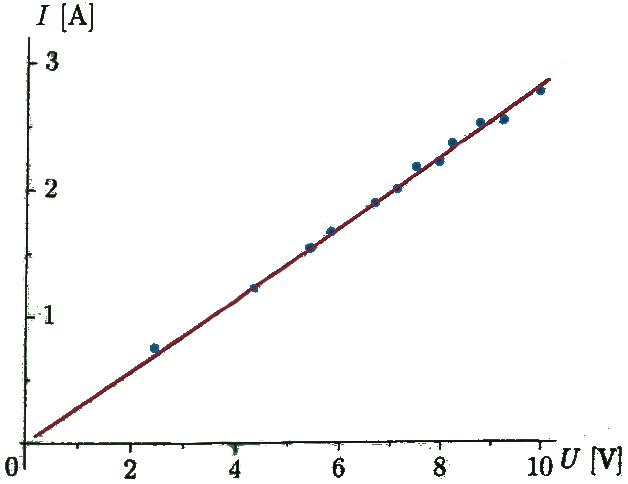
\includegraphics[width=0.8\linewidth]{mai_fig052.png}
  \captionof{figure}{Ověření Ohmová zákona lineární regresí.
  \cite[s.~263]{Musilova2009MA1}
  \label{mai:fig052}}
  \par}
  Pro odpor vychází \(R\doteq\SI{3.52}{\ohm}\). Součet čtverců odchylek přímky se směrnicí \(i/R
  = (1/\num{3.52})\Omega^{-1}\) od souboru bodů grafu je
  \begin{equation*}
    D(R) = \sum_{i=1}^{n}(U_i - R\cdot I_i)^2 \doteq\num{0.01},
  \end{equation*}
  \(\sigma(R) = \sqrt{D(R)/(n-1)}\doteq\sqrt{(\num{0.11}/11)}\doteq\num{0.03}\).  Graf přímky \(U
  = R\cdot I = \num{3.52}\cdot I\) proložené body je na obrázku \ref{mai:fig052}.
\end{mathexam}
      %---------------------------------------------------------------
      
      Popsaný způsob nalezení hodnoty elektrického odporu vodiče se nazývá\textbf{ metodou 
      nejmenších čtverců} (minimalizuje součet čtverců odchylek prokládané závislosti od souboru 
      naměřených bodů), v případě použití lineárního modelu, jako tomu bylo u Ohmová zákona, pak 
      jde o \textbf{lineární regresi}
      
      Obdobně se postupuje, je-li některá z měřených veličin lineární funkcí veličin jiných s 
      neznámými koeficienty lineární kombinace. Nechť
      \begin{equation*}
        Z = f(X_1, X_2, \ldots, X_K) = A_1X_1 + A_2X_2 + \cdots + A_KX_K.
      \end{equation*}
      Předpokládejme, že veličiny \(X_1, X_2, \ldots, X_K\) a \(Z\) měříme \(n\)-krát a naměříme 
      hodnoty
      \begin{equation*}
        X_j = \lbrace x_{j1}, \ldots x_{jn} \rbrace, \qquad 1 \leq j \leq K, \qquad 
        Z = \lbrace z_{1}, \ldots z_{n} \rbrace
      \end{equation*}
      Součet čtverců odchylek teoretické závislosti od naměřených bodů je
      \begin{equation*}
        D(Z) = \sum_{i=1}^{n}\left(z_i - \sum_{j=1}^{K}A_jx_{ji}\right)^2.
      \end{equation*}
      Nutnou podmínkou pro minimum tohoto výrazu jakožto funkce proměnných \(A_x, A_2, \ldots, A_K\)
      je platnost souboru rovnic
      \begin{equation*}
        \pder{D(Z)}{A_p} = 0 \Rightarrow 
        \sum_{i=1}^{n}2\left(z_i - \sum_{j=1}^{K}A_jx_{ji}\right)\cdot x_{pi} = 0
      \end{equation*}
      pro \(1 \leq i \leq n, 1 \leq j \leq K\). Tyto podmínky představují nehomogenní soustavu 
      \(K\) rovnic pro \(K\) neznámých \(( A_1, A_2, \ldots, A_K)\). Rozšířená matice soustavy je
      \begin{equation*}
        \overline{B} = (A|B) = 
          \left(
            \begin{array}{cccc|c}
              \sum_{i=1}^{n}x_{1i}x_{1i} & \sum_{i=1}^{n}x_{1i}x_{2i} & \cdots & 
              \sum_{i=1}^{n}x_{1i}x_{Ki} & \sum_{i=1}^{n}z_{i}x_{1i}                    \\
              \sum_{i=1}^{n}x_{1i}x_{1i} & \sum_{i=1}^{n}x_{2i}x_{2i} & \cdots & 
              \sum_{i=1}^{n}x_{2i}x_{Ki} & \sum_{i=1}^{n}z_{i}x_{2i}                    \\
                        \cdots           & \cdots & \cdots & \cdots   & \cdots          \\
              \sum_{i=1}^{n}x_{Ki}x_{1i} & \sum_{i=1}^{n}x_{Ki}x_{2i} & \cdots & 
              \sum_{i=1}^{n}x_{Ki}x_{Ki} & \sum_{i=1}^{n}z_{i}x_{Ki}                    \\
            \end{array}
          \right),
      \end{equation*}
      \begin{equation*}
        \sigma(z) = \sqrt{\dfrac{D(z)}{n - K}}.
      \end{equation*}
      V dalších kapitolách věnovaných lineární algebře se k tomuto problému znovu vrátíme a 
      ukážeme, že jej lze elegantně řešit také jako úlohu algebraickou, konkrétně úlohu o 
      ortogonální projekci vektorů na podprostory.
      
%} %tikzset
%---------------------------------------------------------------------------------------------------
\printbibliography[heading=subbibliography]
\addcontentsline{toc}{section}{Seznam literatury}
  % % !TeX spellcheck = cs_CZ
%---------------------------------------------------------------------------------------------------
% file: mai1ch07.tex
%---------------------------------------------------------------------------------------------------
%============================ Primitivní funkce ====================================================
\setchaptertoc
\chapter{Poznáváme funkci z její derivace - neurčitý integrál}
  %----------------------------Neurčitý integrál----------------------------------------------------
  \section{Motivace}
    Problém \emph{neurčitého integrálu}, neboli \textbf{primitivní funkce}, lze vyložit velmi 
    jednoduše: Máme podezření, že zadaná funkce \(f(x)\) vznikla derivováním jisté, zatím neznámé, 
    funkce \(F(x)\). Dokážeme ji najít? 
  
    K danému problému můžeme přistupovat také fyzikálně: Zavedením pojmu derivace funkce jsme 
    motivovali důležitým požadavkem definovat okamžitou rychlost pohybu bodu po přímce. Existuje 
    přirozeně i požadavek opačný, tj. nalézt zákon dráhy pohybu bodu po přímce, je-li dána jeho 
    okamžitá rychlost jako funkce času \cite[s.~253]{Brabec1989}. Vše si ukážeme na následujícím 
    příkladu:      
    %-------------------------------------
    % !TeX spellcheck = cs_CZ
%====================== Sbírka řešených příkladů ==================================================
\begin{mathexam}{Je dána okamžitá rychlost \(v\) pohybu bodu po přímce (ose) \(x\) rovnicí \(v(t) =
  2t + 1\), \(t\in\langle -\infty,+\infty \rangle\). Najděte zákon dráhy pohybu, je-li známo, že v
  čase \(t = 0\) měl bod polohu \(x = x_0\) \cite[p.~253]{Brabec1989}.}{exam117}

  Označíme-li \(x(t)\) polohu bodu v okamžiku \(t\), pak \(v(t) = \frac{dx}{dt}\). Hledáme tedy
  funkci \(x = x(t)\), pro níž platí \[\frac{dx}{dt} = 2t + 1 \qquad x(0) = x_0.\] Je ihned patrné,
  že první podmínce vyhovuje nekonečně mnoho funkcí
  \begin{equation}\label{MA:int_ex_09}
    x(t) = t^2 + t + c, 
  \end{equation}
  kde \(c\) je libovolná konstanta. Funkce, která splňuje i druhou podmínku (říkáme ji též počáteční
  podmínka), najdeme z rovnice \ref{MA:int_ex_09} dosazením dané podmínky \(t = 0\), \(x = x_0\).
  Dostaneme \(x_0 = c\). Dosazením do \ref{MA:int_ex_09} za \(c\) plyne hledaný zákon dráhy \(x(t) =
  t^2+t+x_0\).                 

  Jednoduchou zkouškou se přesvědčíme, že tato funkce splňuje obě dané podmínky a zároveň vidíme, že
  hledaná primitivní funkce daných vlastností je jediná.
\end{mathexam}
    %-------------------------------------
    Každé takové funkci, jejíž derivací je daná funkce, budeme říkat \emph{primitivní funkce} k 
    dané funkci. Na uvedeném příkladě je patrné, že k dané funkci může existovat nekonečně mnoho 
    primitivních funkcí. Množinu všech primitivních funkcí se často nazývá \textbf{neurčitým 
    integrálem}. Po tomto názorném uvedení do problému přejděme k přesné formulaci základních pojmů.
    
  \section{Definice primitivní funkce}  
    \begin{mdframed}[style=mdmathdef] 
      \begin{definition}\label{mai:def002}
        Funkci \(F(x): J\rightarrow \realset\), kde \(J\subset \realset\) je interval, nazveme
        \textbf{primitivní} funkcí k funkci \(f(x)\) na intervalu \(J\) právě když, pro všechna
        \(x\in J\) je \(F'(x) = f(x)\). 
        
        V případě uzavřeného intervalu \(J=[a,b]\) požadujeme ještě, aby obě jednostranné derivace
        splňovali \(F_+'(a)=f(a)\) a \(F_-'(b)=f(b)\). 
        
        Množina všech primitivních funkcí k funkci \(f(x)\) na \(J\) se nazývá \textbf{neurčitý
        integrál} z funkce \(f(x)\) a značí se \(\int f(x)\dd{x}\). Tedy
        \begin{gather}\label{mai:eq101}
          \int f(x)\dd{x} = \{F(x): \text{\(F(x)\) je primitivní funkcí k \(f(x)\) na \(J\)}\}
        \end{gather}
      \end{definition}
    \end{mdframed}
    %-------------------------------------
    % !TeX spellcheck = cs_CZ
%====================== Sbírka řešených příkladů ==================================================
\begin{mdframed}[style=mdexam]
  \begin{example}\label{mai:exam118}
    K funkci $\sin x$ je primitivní funkcí na libovolném intervalu $J\subset(-\infty,+\infty)$ 
    funkce $-\cos x$, protože $(-\cos x)' = \sin x$. Ale též funkce $3-\cos x$ je primitivní 
    funkcí k funkci $\sin x$, protože $(3 - \cos x)' = \sin x$ pro všechna $x\in(-\infty, 
    \infty)$.
  \end{example}
\end{mdframed}
    %-------------------------------------
    
    Z uvedených příkladů je vidět, že rozdíl dvou primitivních funkcí k téže funkci je konstanta. To
    není náhoda, jak potvrzuje následující věta:

    \begin{mdframed}[style=mdmathlemma] 
      \begin{lemma}\label{mai:lemma008}(Věta o rozdílu dvou primitivních funkcí)
        \begin{enumerate}[noitemsep]
          \item Je-li funkce $F$ primitivní funkcí k funkci \(f\) na intervalu \(J\) a \(c\) reálná  
                konstanta, pak i funkce $G = F + c$ je primitivní funkcí k funkci \(f\) na intervalu 
                \(J\).
          \item Jsou-li funkce $F$ a $G$ primitivní funkce k funkci \(f\) na intervalu \(J\), pak 
          funkce
                $F-G$ je na intervalu \(J\) konstantní.
        \end{enumerate} 
        \begin{proof}
          Tvrzení a) plyne z definice protože $G'(x) = [F(x) + c] = F'(x) = f(x)$ pro všechna $x\in
          J$. Tvrzení b) je důsledkem věty \ref{MA1:lem_diff01}.
        \end{proof}
      \end{lemma}
    \end{mdframed}

    \subsection{Poznámky k definici}  
      Z definice \ref{mai:def002} vyplývá, že primitivní funkce je spojitou funkcí, neboť má
      derivaci a věta \ref{mai:lemma008} nám říká, že pokud k dané funkci existuje funkce
      primitivní, existuje jich nekonečně mnoho. Je-li např. \(F\) primitivn9 funkce k funkci \(f\)
      na intervalu \(J\), pak množina všech primitivních funkcí je množina \(\{F + c;
      c\in\realset\}\). Tuto množinu označujeme symbolem \(\int f(x)\dd{x}\) a čteme \uv{integrál
      \(f(x)\dd{x})\)} Symbolu \(\int f(x)\dd{x}\) říkáme \textbf{neurčitý integrál}. Zpravidla
      píšeme
      \begin{mdframed}[style=mdmathlemma]  
        \begin{equation}\label{mai:eq102}
          \int f(x)\dd{x} = F(x) + c
        \end{equation}
      \end{mdframed}
      nebo jen \(\int f(x)\dd{x} = F(x)\) (tj. aditivní konstantu vynecháváme) a máme tím na mysli
      že \(F(x) \in \int f(x)\dd{x}\). Rovnost \ref{mai:eq102} je tedy rovnost mezi množinami,
      nikoliv rovnost funkcí. 
    
    \subsection{Některé vlastnosti integrálů}  
      Platnost několika následujících vztahů lze prověřit přímo užitím definic derivace a neurčitého
      integrálu. Tyto vztahy jsou při výpočtech často používány. Nejprve však uvedeme základní
      pravidla pro primitivní funkce, která plynou z pravidel pro derivování:
      \begin{subequations}
        \begin{flalign}
          \int\dd{f(x)} &= f(x) + c,                                          &\label{mai:eq134} \\
          \dxd\left[\int f(x)\dd{x}\right] &= f(x)\dd{x},                     &\label{mai:eq135} \\
          \int[f(x)\pm g(x)]\dd{x}&= \int f(x)\dd{x} + \int g(x)\dd{x},       &\label{mai:eq103} \\
          \int kf(x)\dd{x}      &=k\int f(x)\dd{x},\quad\text{\(k=\) konst.}, &\label{mai:eq104} \\
          \left[\int f(x)\dd{x}\right]' &= f(x),                              &\label{mai:eq136}
        \end{flalign}
      \end{subequations}
  
  \section{Tabulka neurčitých integrálů}\label{MA:chap_tabINT}
    Jak ale primitivní funkce hledat? V jednoduchých příkladech poslouží tabulka derivací, již čteme
    „zprava doleva“. (Je dobré si ji uložit do paměti.) Tabulka však pokryje jen velmi málo případů,
    pouze elementární funkce. Je tedy třeba najít metody, jak při hledání primitivních funkcí
    postupovat.

    Uveďme nyní některé základní integrály. Poznamenejme, že touto tabulkou nejsou zdaleka vyčerpány
    všechny funkce, ke kterým umíme primitivní funkce najít. Existují celé knihy obsahující tabulky
    integrálů a programy výrazně ulehčující hledání primitivních funkcí. Literatura:
    \cite{Rektorys1963}, \cite{Brabec1989}, \cite{diblik2002}. 

    Pokud není nic uvedeno, platí vzorce pro všechna \(x\) a pro všechny hodnoty uvedených konstant.
    Místo platí pro \(x\) z intervalu \((-\infty,0),(0,+\infty)\) píšeme stručně \(x\neq0\) apod.
    Obory platnosti uvádíme jen tam, kde nejsou evidentní.  

    \begin{flalign}
      \midrule
      & \int 0\dd{x} = c                                        &      \label{mai:eq105}     \\
      & \int a\dd{x} = ax+c                                     &      \label{mai:eq106}     \\
      & \int x^n\dd{x} = \frac{x^{n+1}}{n+1}+c,                 &      \label{mai:eq107}     \\              
        \shortintertext{\hspace{2em} kde \(\begin{cases}
          \forall x\in\realset,\,n\in\naturalset, n>0,         \\
          \forall x\in\realset-\{0\},\,n\in\naturalset, n<-1,  \\
          \forall x>0,\,n\in\realset\,\,n\neq-1
        \end{cases}\)}                                          
      & \int\frac{1}{x}\dd{x} = 
            \ln\abs{x}+c \hspace{1ex}\forall x\neq0            &       \label{mai:eq108}    \\
      & \int e^x \dd{x}       = e^x+c                          &       \label{mai:eq109}    \\
      & \int\ln x\dd{x}       = 
          x\ln x - x + c \hspace{1ex}\forall x>0               &       \label{mai:eq110}    \\
      & \int a^x \dd{x}     =
        \frac{a^x}{\ln a}+c 
        \hspace{1ex}\forall a>0,\,a\neq1                       &       \label{mai:eq111}    \\
      & \int \sin x \dd{x}  = -\cos x                          &       \label{mai:eq112}    \\
      & \int \cos x \dd{x}  =  \sin x                          &       \label{mai:eq113}    \\
      & \int\frac{1}{\cos^2x}\dd{x} =  \tan x + c              &       \label{mai:eq114}    \\
        \shortintertext{\(\hspace{2em}\forall x\neq\frac{1}{2}\pi+k\pi,\,k\in\naturalset\)}\nonumber\\       
      & \int\frac{1}{\sin^2x}\dd{x}     =  -\cotg x+c         &        \label{mai:eq115}    \\
        \shortintertext{\(\hspace{1em}\forall x\neq k\pi,\,k\in\naturalset\)}
      & \int\frac{1}{\sqrt{1-x^2}}\dd{x} =
          \begin{cases}
            +\arcsin x + c         \\
            -\arccos x + c
          \end{cases}                                          &      \label{mai:eq116}    \\
        \shortintertext{\(\hspace{2em}\forall x\in(-1,1) \)}  
    & \int\sinh x\dd{x} = \cosh x + c                         &       \label{mai:eq117}    \\
    & \int\dfrac{1}{\sinh x}\dd{x} = -\cotgh x + c            &       \label{mai:eq118}    \\
    & \int\cosh x\dd{x} = \sinh x + c                         &       \label{mai:eq119}    \\
    & \int\dfrac{1}{\cosh x}\dd{x} = -\tanh x + c             &       \label{mai:eq120}    \\
    & \int\frac{1}{1+x^2}\dd{x} = \arctan x + c               &       \label{mai:eq121}    \\
    & \int\frac{1}{\sqrt{x^2 + 1}}\dd{x} =
        \begin{cases}
            \ln(x + \sqrt{x^2+1}) + c         \\
            \arcsinh x            + c 
        \end{cases}                                           &       \label{mai:eq122}    \\ 
    & \int \frac{1}{\sqrt{x^2 - 1}}\dd{x} =
        \begin{cases}
            \ln(x + \sqrt{x^2-1}) + c         \\
            \arccosh x            + c  
        \end{cases}                                           &       \label{mai:eq123}    \\   
      \shortintertext{\hspace{2em}\(x\in(1,+\infty)\)}  
    & \int\frac{1}{\sqrt{x^2+a^2}}\dd{x} 
        = \begin{cases}
              \arcsinh\frac{x}{a}   + c  \\ 
              \ln(x+\sqrt{x^2+a^2}) + c     
          \end{cases}                                          &      \label{mai:eq124}    \\
    & \int \frac{1}{\sqrt{x^2-a^2}}\dd{x} 
        = \begin{cases}
              \arccosh\frac{x}{a}   + c   \\
              \ln(x+\sqrt{x^2-a^2}) + c
          \end{cases}                                          &      \label{mai:eq125}    \\
    & \int\tan x \dd{x}   = \ln\abs{\sec x} + c                &      \label{mai:eq126}    \\
    & \int\sec x \dd{x}   = \ln\abs{\sec x + \tan x} + c       &      \label{mai:eq127}    \\
    & \int\sec^2 x \dd{x} = \tan x + c                         &      \label{mai:eq128}    \\
    & \int\sec x\tan x \dd{x} = \sec x + c                     &      \label{mai:eq129}    \\
    & \int\frac{a}{a^2+x^2}\dd{x} = \tan^{-1}\frac{x}{a} + c   &      \label{mai:eq130}    \\
    & \int\frac{a}{a^2-x^2}\dd{x} = 
      \frac{1}{2}\ln\left\lvert\frac{x+a}{x-a}\right\rvert     &      \label{mai:eq131}    \\
    & \int\frac{1}{\sqrt{a^2-x^2}} \dd{x} = 
      \sin^{-1} \frac{x}{a}                                    &      \label{mai:eq132}    \\
    & \int\frac{a}{x\sqrt{x^2-a^2}}\dd{x} = 
      \sec^{-1} \frac{x}{a}                                    &      \label{mai:eq133}    \\
      \midrule  
    \end{flalign}

    \begin{mdframed}[style=mdmathlemma]  
      \(\argsinh x\), \(\argcosh x\), \(\argtanh x\), \(\argcoth x\) jsou funkce inverzní k
      hyperbolickým funkcím. Značení těchto funkcí není jednotné. Správné zkratky jsou ty, které
      specifikuje norma \texttt{ISO 80000-2}. Skládají se z \uv{ar} následovaných zkratkou
      odpovídající hyperbolické funkce (např. arsinh, arcosh).

      Nicméně, předpona \uv{arc} - následovaný odpovídající hyperbolickou funkcí (např. arcsinh,
      arccosh) je také běžně vidět, analogicky s nomenklaturou pro inverzní trigonometrické funkce.
      Není to však správné pojmenování, protože prefix \uv{arc} je zkratka pro \textbf{arcus},
      zatímco prefix \uv{ar} znamená \textbf{area}. 

      Autoři jako prof. K. Rektorys upřednostňují použití označení \(\argsinh\), \(\argcosh\),
      \(\argtanh\) atd., kde předpona \uv{arg} je zkratkou latinského \textbf{argumentu}. V
      počítačové vědě se to často zkracuje na asinh.

      Používá se také zápis \(\sinh^{-1}(x)\), \(\cosh^{-1}(x)\) atd., a to navzdory skutečnosti, že
      je třeba dbát na to, aby nedošlo k nesprávným interpretacím horního indexu \(-1\) jako
      mocniny, na rozdíl od zkratky pro označení inverzní funkce (např.\(\cosh^{-1}(x)\) versus
      \(\cosh(x)^{-1}\)).
    \end{mdframed}

  \twocolumn[\section{Metody určení primitivní funkce}]
    Procesu hledání primitivní funkce se často říká integrování nebo integrace (od slova“integrál”),
    což z matematického hlediska znamená provést inverzní operaci k operaci derivování. Smutnou
    zprávou je, že na rozdíl od derivování neexistuje obecný vzorec pro integrování součinu či
    podílu, ani obecný vzorec pro integrování složených funkcí. Při hledání integrálů složitějších
    funkcí se využívá např. \emph{linearita, metoda per partes, substituční metoda}, popř. některé
    další speciální metody. Řešitel v mnoha případech musí projevit důvtip a intuici, která mu
    pomůže nalézt primitivní funkci k dané funkci.
  
    % --------------------------Integrace po částech - per partes-----------------------------------
    \subsection{Integrace po částech - per partes}
      Metoda integrace \emph{per partes} neboli \emph{po částech} využívá vzorce pro derivaci 
      součinu funkcí. Připomeňme si jej: Pro derivaci součinu dvou funkcí \(u(x)\) a \(u(x)\) platí
      \cite[p.~137]{Musilova2009MA1}.
      \begin{equation}\label{MA:eq_Int29}
        [u(x)v(x)]' = u(x)'v(x) + u(x)v'(x).
      \end{equation} 
      Primitivní funkcí levé strany je \(F(x) = u(x)v(x)\), a tedy
      \begin{equation*}
        u(x)v(x) =  \int u'(x)v(x)\dd{x} + \int u(x)v'(x)\dd{x}
      \end{equation*}  
      za předpokladu, že existují obě primitivní funkce na pravé straně. K čemu může tento
      samozřejmý vzorec sloužit při hledání primitivní funkce? Dejme tomu, že zadaná funkce
      \(f(x)\), k níž máme hledat funkci primitivní, je tvaru \(f(x) = u'(x)v(x)\), a my si s ní
      nevíme rady. Je však možné, že bychom si docela dobře poradili s primitivní funkcí k funkci
      \(g(x) = u(x)v(x)\). A předchozí vzorec umožňuje nahradit výpočet neurčitého integrálu z
      funkce \(f(x)\) výpočtem neurčitého integrálu z funkce \(g(x)\), tedy
      \begin{equation}\label{ma:eq_perpartes}
        \int u'(x)v(x)\dd{x} = u(x)v(x) - \int u(x)v'(x)\dd{x} 
      \end{equation}

      %-------------------------------------
      \begin{mathexam}{\(\int x\sin x\dd{x}\)}{exam111} 
  
  Součin v zadání je zřejmý. Můžeme si zvolit buď \(u=x\) a \(v'=\sin x\), nebo naopak \(u=\sin x\)
  a \(v'= x\).
  
  Zkusíme nejprve první volbu. Je-li \(u=x\) bude \(u=1\). Dále \(v'=\sin x\), tedy \(v=\int\sin
  x\dd{x} = -\cos x\) (integrační konstantu volíme rovnou nule, stačí nám jedna konkrétní primitivní
  funkce). Ze vzorce \eqref{mai:eq147} dostaneme
  \begin{align*}
    \int x\sin x\dd{x} &= x(-\cos x) - \int1\cdot(-\cos x)\dd{x} \\
                       &= -x\cos x + \sin x + c.
  \end{align*}  
  Tato volba tedy vedla k cíli. Výpočet obvykle zapisujeme do jakési tabulky, takže zápis vypadá
  následovně:
  \begin{align*}
    \int x\sin x\dd{x} &= %
      \left\lvert
        \begin{matrix} 
          u = x     & u' =1        \\
          v'=\sin x & v  = -\cos x 
        \end{matrix}  
      \right\rvert =                                              \\
                       & = x(-\cos x) - \int1\cdot(-\cos x)\dd{x} \\
                       &= -x\cos x + \sin x + c.
  \end{align*}  
\end{mathexam}
      %-------------------------------------

      Není vždy jednoduché rozpoznat, jak máme rozložit funkci \(f(x)\) na součin funkcí \(u'(x)\) 
      a \(v(x)\). Takový rozklad není určen jednoznačně a požadavek na něj bychom mohli (dosti 
      nepřesně) formulovat tak, aby funkce \(v'(x)\) byla jednodušší než v \(v(x)\) (například 
      derivováním polynomu se snižuje jeho stupeň) a funkce \(u'(x)\) a \(u(x)\) aby byly zhruba 
      „stejně složité“ (například \(u'(x) =e^x\), \(u(x) = e^x\), nebo \(u'(x) = \cos x\), \(u(x) = 
      \sin x\), apod.). Spolehlivě používat metodu per partes se však můžeme naučit pouze studiem 
      vyřešených příkladů z literatury a praktickým procvičováním \cite[p.~138]{Musilova2009MA1}.
  
      %-------------------------------------
      \begin{mdframed}[style=mdexam]
  \begin{example}\label{mai:exam109}
    (\emph{Umělý rozklad na součin}): Někdy zadaná funkce \(f(x)\) jako součin vůbec nevypadá, a
    přesto je použití metody per partes vhodné. Například pro elementární funkci \(f(x) = \ln x\)
    sice najdeme primitivní funkci \ref{MA:baseInt06} v tabulce základních neurčitých integrálů z
    odstavce \ref{MA:chap_tabINT}, ale je možné postupovat i jinak. Představme si \(f(x)\) jako
    součin \(f(x) = 1\cdot\ln x\) a zvolme \[u'(x) = 1 ⇒ u(x) = x, \quad v(x) = lnx ⇒ v'(x) =
    \frac{1}{x}\] Pak 
    \begin{align*}
      \int\ln\dd{x} &= x\ln x - \int x\cdot\frac{1}{x}\dd{x}  \\ 
                    &= x\ln x - x.
    \end{align*}
  \end{example}
\end{mdframed}
      %-------------------------------------
  
    %--------------------------- Substituční metoda ----------------------------------------------
    \subsection{Substituční metoda I}
      Tato metoda \emph{substituce} neboli \emph{náhrady} spočívá v tom, že vhodně zvolenou funkci
      obsaženou v předpisu \(f(x)\) označíme jako novou jednoduchou proměnnou. Čeho tím dosáhneme?
      Předpokládejme například, že \[f(x)=\varphi'(x)g[\varphi(x)]\] a označme jako novou proměnnou
      \(u = f(x)\). Že to vypadá, jako bychom se chystali použít vzorec pro derivaci složené funkce?
      Správně! Dejme tomu, že známe primitivní funkci \(G(u)\) k funkci \(g(u)\). Pak platí
      \begin{equation*}
        \left[G\left(\varphi(x)\right)\right]' = G'\left[\varphi(x)\right]\cdot\varphi'(x) 
        = g\left[\varphi(x)\right]\cdot\varphi'(x),     
      \end{equation*}
      a tedy
      \begin{equation*}
        \int \varphi'(x) g\left[\varphi(x)\right]\dd{x} =  G\left[\varphi(x)\right]. 
      \end{equation*}      
      Na základě těchto úvah formulujeme následující větu (viz. \cite[p.~142]{diblik2002}):
      \begin{mdframed}[style=mdmathlemma]
        \begin{lemma}\label{mai:lemma009}
          Jestliže
          \begin{equation}\label{ma:eq_subst1}
            \int{f(u)\dd{u}}=F(u)+c
          \end{equation}
          a $u=\varphi(x)$, pak
          \begin{equation}\label{ma:eq_subst2}
              \int{f[\varphi(x)]\varphi'(x)\dd{u}}=F(\varphi(x))+c
          \end{equation}
        \end{lemma}
      \end{mdframed}
  
      Základem úspěchu při aplikací věty je správný výběr funkce $\varphi(x)$. Praxe je totiž
      taková, že výpočet konkrétních příkladů je schématicky veden od rov. \ref{ma:eq_subst2} ke
      vzorci rov. \ref{ma:eq_subst1}.

      %-------------------------------------
      \begin{mdframed}[style=mdexam]
  \begin{example}\label{MAI:exam110}
    Jak poznat kandidáta na substituční metodu I. Počítejme neurčitý integrál 
    \begin{equation*}
      \int\frac{x}{\sqrt{x^2+1}}\dd{x}.
    \end{equation*} 

    \noindent\textbf{Řešení:}

    Vidíme, že čitatel funkce za integrálem je až na násobení konstantou \((2)\) derivací výrazu pod
    odmocninou. Při označení \(u=\varphi(x) = x^2 + 1\) dostáváme \(\varphi'(x) = x\) a řešíme
    následující integrál:
    \begin{gather*}
      \frac{1}{2}\int\frac{2x}{\sqrt{x^2+1}}\dd{x} 
        = \frac{1}{2}\int\frac{1}{\sqrt{u}}\dd{u} = \sqrt{u} + c    
        = \sqrt{x^2 + 1} + c.  
    \end{gather*}
  \end{example}
\end{mdframed}
      %-------------------------------------

      %-------------------------------------
      \begin{mdframed}[style=mdexam]
  \begin{example}\label{MAI:exam124} 
    Řešme: 
    \begin{equation*}
      \int\sin^3t\cos t\dd{t}.
    \end{equation*}

    \noindent\textbf{Řešení:}

    Položme \(\sin t = x\), \(\cos t\dd{t} =\dd{x}\). Pak získáme triviální integrál
    \begin{equation*}
      \int x^3\dd{x} = \frac{1}{4}x^4 + c = \frac{1}{4}\sin^4t + c,
    \end{equation*}
    Podmínky věty jsou splněny: Funkce \(\sin t\) je na intervalu \(-\infty, +\infty\) spojitá i se
    svou derivací \(\cos t\), její hodnoty leží v intervalu \(\langle-1,1\rangle\). V tomto
    intervalu je funkce \(x^3\) spojitá \cite[s.~261]{Brabec1989}. 
  \end{example}
\end{mdframed}
      %-------------------------------------

      %-------------------------------------
      \begin{mathexam}{\(\protect\scalerel{\int}{(1+x^2)^5x\dd{x}}\)
  \hfill\cite[s.~261]{Brabec1989}.}{exam125} 
  
  Zavedeme substituci \(1+x^2 = u\); odftud \(2x\dd{x} = \dd{u}\), tj. \(x\dd{x}=\frac{1}{2}\dd{u}\)
  (používáme jiné označení proměnných než je v uvedené větě). Potom platí 
  \begin{equation*}
    \frac{1}{2}\int u^5\dd{u} = \frac{1}{12}u^6 + c = \frac{1}{12}(1+x^2)^6 + c,
  \end{equation*}
  kde \(x\in(-\infty, +\infty)\), \(u\in\langle 1,+\infty)\); podmínky věty o substituci jsou
  zřejmě splněny.  
\end{mathexam}
      %-------------------------------------      

      %-------------------------------------
      \begin{mathexam}{Nechť \(\int{f(x)}\dd{x} = F(x) + c, \quad a,b\in\realset, a\neq0\)
  \hfill\cite[s.~261]{Brabec1989}.}{exam126}
  Pak platí
  \begin{equation}\label{mai:eq138}
    \int{f(ax + b)}\dd{x} = \frac{1}{a}F(ax + b) + c.
  \end{equation}
  Položíme \(ax + b =z\). Odtud \(a\dd{x} = \dd{z}\), \(\dd{x} = \frac{1}{a}\dd{z}\); 
  \begin{equation*}
    \boxed{\frac{1}{a}\int{f(z)}\dd{z} = \frac{1}{a}F(z) + c = \frac{1}{a}F(ax+b) + c.}
  \end{equation*}
  Například \(\int{\sin(2x+1)}\dd{x} = -\frac{1}{2}\cos(2x + 1) + c\) nebo \(\int{e^{-x}}\dd{x} =
  -e^{-x} + c\). 
\end{mathexam}
      %------------------------------------- 

      %-------------------------------------
      \begin{mdframed}[style=mdexam]
  \begin{example}\label{MAI:exam119}
    Cvičení:
    \begin{enumerate}[label=\alph*)]
      \item \(\displaystyle\int x\cdot e^{x^2}\dd{x}\)
      \item \(\displaystyle\int x^3\cdot e^{x^4}\dd{x}\)
    \end{enumerate}

    \noindent\textbf{Řešení:}

    \begin{enumerate}[label=\alph*)]
      \item Položme \(u=x^2\) potom dostaneme diferenciál \(\dd{u}=2x\dd{x}\). Podmínky věty jsou
            splněny. Funkce \(x^2\) je spojitá, včetně derivace \(x\). Dostáváme
            \(\frac{1}{2}\int{e^u\dd{u}}=\frac{1}{2}e^u=\frac{1}{2}e^{x^2} + c\). 
      \item Podobně \(u=x^4 \Rightarrow \dd{u}=4x^3\dd{x}\). Dostáváme 
            \(\frac{1}{4}\int{e^u}\dd{u} = \frac{e^u}{4} = \frac{e^{x^4}}{4} + c \).
    \end{enumerate}
  \end{example}
\end{mdframed}
      %-------------------------------------

      Ukažme, že platí 
      \begin{equation}\label{mai:eq139}
        \boxed{\int{\dfrac{f'(x)}{f(x)}}\dd{x} = \ln\abs{f(x)} + c.}
      \end{equation}
      Zavedeme substituci \(f(x) =t\), pak \(f'(x)\dd{x} = \dd{t}\) a 
      \begin{equation*}
        \int{\dfrac{\dd{t}}{t}} = \ln\abs{t} + c = \ln\abs{f(x)} + c
      \end{equation*}
      na každém intervalu, v němž \(f(x)\neq 0\) a existuje \(f'\). Připomeňme, že výraz
      \(\dfrac{f'(x)}{f(x)}\) se nazývá \emph{logaritmická derivace funkce} \(f\). Viz příklad
      \ref{mai:exam123}.
   

    % -------------------Substituční metoda II------------------------------------------------------
    \newpage
    \subsection{Substituční metoda II}
      Druhý typ substituční metody spočívá naopak v tom, že na místo původní proměnné \(x\) 
      dosadíme vhodnou funkci \(x = \psi(t)\). Místo primitivní funkce k funkci \(f(x)\) pak 
      hledáme primitivní funkci k funkci \(g(t) = f[\psi(t)]\psi'(t)\). Skutečně, je-li \(F(x)\) 
      primitivní funkcí k \(f(x)\), pak derivací složené funkce \(G(t) = F[\psi(t)]\) dostaneme
      \begin{equation*}
       G'(t) = F'[\psi(t)]\psi'(t) = f[\psi(t)]\psi'(t) = g(t).
      \end{equation*}

      %-------------------------------------
      \begin{mathexam}{Náhrada proměnně \(x\) funkcí. Typické jsou neurčité integrály, které vedou na
  goniometrické substituce, například \[\int\sqrt{1-x^2}\dd{x}\]}{exam122}
    
  Označme \(x=\psi(t)=\sin(t)  \Rightarrow \psi'(t)=\cos(t)\). Budeme potřebovat také základní
  goniometrické vzorce (\ref{MA1:eq_sincos},\ref{MA1:eq_cos2x} a \ref{MA1:eq_sin2x}). Můžeme psát
  \begin{gather*}
    \int\sqrt{1-\sin^2t}\cos t\dd{t} 
      = \int\cos^2 t \dd{t}  = \int\frac{1+\cos2t}{2}\dd{t}                         
  \end{gather*}
  Dostáváme
  \begin{align*}
      &= \frac{1}{2}t+\frac{\sin2t}{4}+c                       \\
      &= \frac{1}{2}\arcsin x + \frac{2\sin t\cos t}{4}        \\
      &= \frac{1}{2}\arcsin x + \frac{x\sqrt{1-x^2}}{2} + c.
  \end{align*}
  Správně bychom měli místo \(\sqrt{1 - \sin^2x}\) psát \(\abs{\cos x}\). Vzhledem k tomu, že jde o
  neurčitý integrál, je možné hledat primitivní funkci na intervalu, kde platí \(\cos x = \abs{\cos
  x}\).
\end{mathexam}
      %-------------------------------------

      Jistě nám neuniklo, že princip substitučních metod I a II je stejný. Jsou totiž obě založeny 
      na použití pravidla pro derivaci složené funkce.
  
    % ---------Integrování součtu, úprava integrandu a integrování rozkladem------------------------
    \twocolumn[\subsection{Integrování součtu, úprava integrandu a integrování rozkladem}]
      %-------------------------------------
      \begin{mdframed}[style=mdexam]
  \begin{example}\label{MAI:exam121}
    Zdroj \cite[s.~29]{Knichal}.
    \begin{equation}\label{MA:int_ex_01}
      \int{\frac{x^4+3x^3-3x^2+3x}{x^2+1}\dd{x}}
    \end{equation}
    Dělením čitatele integrandu jmenovatelem  dostaneme rozklad integrandu na součet funkcí,
    jejich integrály najdeme snadno:
    \begin{equation*}
      \rotatebox{90}{$
        {\polylongdiv[style=C,div=:]{x^4+3x^3-3x^2+3x}{x^2+1}}
      $}
    \end{equation*}

    Tedy
    \begin{equation*}
      \frac{x^4+3x^3-3x^2+3x}{x^2+1} = x^2+3x-4+\frac{4}{x^2+1}  
    \end{equation*}
    Pro uvedený integrál dostaneme
    \begin{align*}
      \int{x^2}\dd{x} &+\int{3x}\dd{x}-4\int\dd{x}+\int{\frac{4}{x^2+1}\dd{x}} \\
                      &= \frac{x^3}{3}+\frac{3x^2}{2}-4x+4\arctan x + c.
    \end{align*}
  \end{example}
\end{mdframed}
      %-------------------------------------
      
      \begin{example}
        Zdroj \cite[s.~29]{Knichal}.
        \begin{equation}\label{MA:int_ex_02}
          \int\frac{3}{(1+x^2)x^2}\dd{x}
        \end{equation}
        Integrand upravíme přičtením a odečtením výrazu $3x^2$ v čitateli zlomku takto:
        \begin{align*}
          \frac{3}{(1+x^2)x^2} 
            &= \frac{3+3x^2-3x^2}{(1+x^2)x^2} = \frac{3}{x^2}-\frac{3}{1+x^2}                      \\  
          \intertext{Tedy v každém otevřeném intervalu, který neobsahuje bod \(x=0\), platí}
          \int{\frac{3}{(1+x^2)x^2}\dd{x}} 
            &= 3\int{\frac{1}{x^2}dx} - 3\int{\frac{1}{1+x^2}dx}                                   \\
            &= -\frac{3}{x}-3\arctan x + c. 
        \end{align*}
      \end{example}
      
      \begin{example}
        Zdroj \cite[s.~30]{Knichal}.
        \begin{equation}\label{MA:int_ex_04}
          \int{\sqrt{1+\cos2x}\dd{x}}
        \end{equation}
        Funkci $\sqrt{1+\cos2x}$ upravíme na základě goniometrické identity \ref{MA1:eq_cos2x}:
        \(1+\cos2x = 1+\cos^2x-\sin^2x=2\cos^2x\) takto
        \begin{equation*}
          \sqrt{1+\cos2x} =\sqrt{2\cos^2x} = \sqrt{2}\abs{\cos x} = \varepsilon\sqrt{2}\cos x, 
        \end{equation*}
        \begin{equation*}
          \text{kde}\,\varepsilon =
            \begin{cases} 
             +1, &  x\in \left(-\frac{\pi}{2}+2n\pi,\frac{\pi}{2}+2n\pi\right), \\
             -1, &  x\in \left(\frac{\pi}{2}+2n\pi,\frac{3\pi}{2}+2n\pi\right),
            \end{cases}
        \end{equation*}
        $n$ je přirozené číslo. Proto pro $x$ ležící v uvedených intervalech je
        \begin{equation*}
          \int\sqrt{1+\cos2x}\dd{x} = \varepsilon\sqrt{2}\int\cos x\dd{x} 
                                 = \varepsilon\sqrt{2}\sin x + c.
        \end{equation*}
      \end{example}
      
      \begin{example}Zdroj \cite[s.~30]{Knichal}.
        \begin{equation}\label{MA:int_ex_05}
          \int\cos^2\frac{x}{2}\dd{x}
        \end{equation}
        Integrand upravíme na součet dvou tabulkových integrálů použitím vzorce
        \begin{align*}
          \cos^2\frac{x}{2} &= \frac{1}{2}(1+\cos x)     \\ 
          \shortintertext{takže}
          \int{\cos^2\frac{x}{2}}\dd{x} 
                            &= \frac{1}{2}\int{(1+\cos x)}\dd{x} = \frac{1}{2}(x+\sin x) + c.
        \end{align*}          
      \end{example}
      
      \begin{example}
        Zdroj \cite[s.~30]{Knichal}.
        \begin{equation}\label{MA:int_ex_06}
          \int{\tan^2x}\dd{x}
        \end{equation}
        funkci napíšeme ve tvaru 
        \begin{align*}
          \tan^2x &= \frac{\sin^2x}{\cos^2x}=\frac{1-\cos^2x}{\cos^2x} = \frac{1}{\cos^2x}-1   \\
          \shortintertext{takže}
          \int{\tan^2x}dx &= \int{\left(\frac{1}{\cos^2x}-1\right)}\dd{x} = \tan x - x + c.  
          \intertext{$\forall x\in\left(-\frac{\pi}{2}+k\pi, \frac{\pi}{2}+k\pi\right)$,
                     $k\in\naturalset$.}
        \end{align*}        
      \end{example}
      
      \begin{example}
        \begin{equation}\label{MA:int_ex_07} 
          \int\frac{\cos2x}{\cos^2x\cdot\sin^2x}\dd{x}, 
        \end{equation} 
        Je-li \(\sin^2x\cos^2x\neq0;\, x\neq k\frac{\pi}{2};\, k\in Z\).
        Integrand upravíme pomocí vzorce pro dvojnásobný úhel \ref{MA1:eq_cosx2}:
        \begin{align*}
          \int\frac{\cos^2x-\sin^2x}{\cos^2x\cdot\sin^2x}\dd{x} 
             &= \int\frac{1}{\sin^2x}\dd{x} -\int\frac{1}{\cos^2x}\dd{x}        \\
             &= -\cot x - \tan x + c. 
        \end{align*}
      \end{example}
      
      \begin{example}
       \begin{equation}\label{MA:int_ex_08}
         \int\frac{1}{\cos x\cdot\sin x}\dd{x}, 
       \end{equation}
       \((\sin x\cos x\neq0; x\neq k\frac{\pi}{2}; k\in Z)\).
       Integrand rozšíříme o funkci $\displaystyle{\frac{1}{\cos^2x}}$
        \begin{equation*}
          \bigintss\dfrac{\dfrac{1}{\cos^2x}}{\dfrac{\sin x\cdot\cos x}{\cos^2x}} \dd{x} = 
          \bigintss\dfrac{\dfrac{1}{\cos^2x}}{\tan x}\dd{x} = \ln\abs{\tan x} + C.
        \end{equation*}            
      \end{example}
  
    %--------------------------- Integrace racionální funkce--------------------------------------
    \newpage
    \subsection{Integrace racionální funkce}
      Některé příklady v předchozím odstavci, (viz např. \ref{MA:int_ex_01} a 
      \ref{MA:int_ex_02}) jsme dělením čitatele integrandu jmenovatelem dostali rozklad
      integrandu na součet racionální funkce (polynomu) a ryze lomené racionální funkce.
      Integrování polynomu je snadné, neboť jde o součet integrálů tvaru $\int c_kx^k dx$, kde
      $k$ je celé nezáporné číslo. Omezíme se tedy na integrování \emph{ryze lomené racionální
      funkce},  tj. funkce ve tvaru $P(x)/Q(x)$, kde $P(x), Q(x)$ jsou polynomy, přičemž stupeň
      polynomu $P(x)$ je menší než stupeň polynomu $Q(x)$. Taková funkce může vzniknout součtem
      několika jednoduchých zlomků (viz. následující příklad \ref{MAI:exam116}).
      
      %-------------------------------------
      \begin{mdframed}[style=mdexam]
  \begin{example}\label{MAI:exam116}
    Upravte
    \begin{align*}
      \frac{1}{x-1}+\frac{x+2}{x^2+x+3} 
        &= \frac{x^2+x+3+x^2+x-2}{(x-1)(x^2+x+3)}                \\
        &= \frac{2x^2+2x+1}{x^3+2x-3}
    \end{align*}  
  \end{example}
\end{mdframed}
      %-------------------------------------
      
      Jsme tedy vedeni myšlenkou, zda naopak každá ryze lomená racionální funkce se dá rozložit
      na součet jednoduchých zlomků určitého tvaru - budeme jim říkat \textbf{parciální zlomky},
      které umíme integrovat. Tím se budeme zabývat v dalších odstavcích. 
    
      %-------------------------------------
      \begin{mdframed}[style=mdexam]
  \begin{example}\label{MAI:exam120}
    Řešme integrál 
    \begin{equation*}
      \int\frac{1}{x^2 - x + 1}\dd{x}, \qquad x\in\realset:
    \end{equation*}
    \noindent\textbf{Řešení:}

    Kvadratický polynom ve jmenovateli upravíme na čtverec \(f(x) = (x + m)^2 + n\) a dostaneme
    integrál
    \begin{equation*}
      \int\dfrac{1}{\left(x-\dfrac{1}{2}\right)^2+\dfrac{3}{4}}\dd{x},
    \end{equation*}
    na který lze aplikovat vzorec \ref{mai:eq121} z tabulky neurčitých integrálů: 
    \begin{equation*}
      \dfrac{1}{\sqrt{1-\left(\dfrac{1}{2}\right)^2}}\arctan
      \dfrac{x-\dfrac{1}{2}}{\sqrt{1-\left(\dfrac{1}{2}\right)^2}} 
    \end{equation*}
    \begin{equation*}
      \dfrac{2}{\sqrt{3}}\arctan\dfrac{2x-1}{\sqrt{3}}  =
      \dfrac{2\sqrt{3}}{3}\arctan\dfrac{\sqrt{3}(2x-1)}{3} + c
    \end{equation*}
  \end{example}
\end{mdframed}
      %-------------------------------------
      
      \begin{mdframed}[style=mdmathdef] 
        \begin{definition} Parciální (částečným) zlomkem, budeme nazývat zlomek tvaru
          \begin{equation}
              \frac{A}{(x-\alpha)^k} \qquad\text{nebo}\qquad\frac{Mx + N}{x^2 + px +q}
          \end{equation}  
          $A,\ M,\ N,\ \alpha\ , p,\ q$ reálné $p^2-4q < 0$, $k$ celé nezáporné.         
        \end{definition}
      \end{mdframed}    
      
      Integrál prvního zlomku, vypočteme substitucí $x-\alpha=t$, odtud plyne \(\dd{x} = \dd{t}\),
      \begin{equation}\label{MA:int_ex_14}
        \boxed{\int\frac{A}{(x-\alpha)^k}dx = \int\frac{A}{t^k}dt.}
      \end{equation}
      Tento integrál se rovná
      \begin{equation}\label{MA:int_ex_16}
        -\frac{A}{k-1}\frac{1}{(x-\alpha)^{k-1}} + C, \quad k\neq1.
      \end{equation}  
      a 
      \begin{equation}
        A\ln\abs{x-\alpha} + C, \quad k = 1
      \end{equation}      
      Výsledek platí na každém intervalu neobsahujícím bod \(\alpha\).
      
       U integrálu druhého zlomku 
       \begin{equation}\label{mai:eq137}
        \boxed{\int{\frac{Mx + N}{x^2+px+q}dx}}
      \end{equation} 
       uvedeme postup výpočtu pro $k = 1$. Předpokládáme samozřejmě, že kvadratický trojčlen
       \(x^2+px+q\) nemá kořeny v reálném oboru, takže jej nelze rozložit do tvaru \((x - \alpha)(x
       - \beta)\) s reálnými \(\alpha\), \(\beta\) (\cite[p.~140]{Musilova2009MA1}). Platí 
      \begin{equation*}
        \frac{Mx}{x^2+px+q} 
          = \frac{M}{2}\frac{2x +b}{x^2+px+q} + \left(b - \frac{MN}{2}\right)\frac{1}{x^2+px+q}
      \end{equation*} 
      \begin{align*}
        \quad &=   \int{\frac{Mx}{x^2+px+q}dx} + \int{\frac{N}{x^2+px+q}dx}     \\  
        \quad &=   \frac{M}{2}\int{\frac{(2x + p) - p}{x^2+px+q}dx} + 
                  N\int{\frac{1}{x^2+px+q}dx}                                   \\ 
        \quad &=   \frac{M}{2}\int{\frac{2x + p}{x^2+px+q}dx} + 
                  \left(N-\frac{Mp}{2}\right)\int{\frac{1}{x^2+px+q}dx.}                   
      \end{align*}  
      
      Z naznačeného postupu je vidět hlavní myšlenka: upravit integrál na lineární kombinaci dvou
      integrálů, z nichž první má v čitateli integrandu derivaci jmenovatele stává kandidátem na
      použití substituční metody I. Je tedy roven $\ln\abs{x^2+px+q}$ kde $x^2+px+q >0$ pro $x\in R$
      a integrand druhého integrálu má čitatel konstantní.
      
      Výpočet druhého integrálu probíhá takto: 
      \begin{equation}\label{MA:int_ex_10}
        \int\dfrac{1}{x^2+px+q}\dd{x} = 
          \int\dfrac{1}{\left(x+\dfrac{p}{2}\right)^2 + q - \dfrac{p^2}{4}}\dd{x};
      \end{equation}
      substitucí $x+\dfrac{p}{2} = t\sqrt{q - \dfrac{p^2}{4}}$ dostáváme dále
      \begin{equation*}\label{MA:int_ex_11}
        \bigints{\frac{1}{\displaystyle{\left(x+\frac{p}{2}\right)^2 + q - \frac{p^2}{4}}}}dx 
          =\displaystyle{
            \bigints{
              \frac{\sqrt{q-\frac{p^2}{4}}}{\left(q-\frac{p^2}{4}\right)(t^2+1)}}dt
            }   
      \end{equation*}
      po úpravě dostaneme tabulkový integrál
      \begin{equation}\label{MA:int_ex_12}
        \frac{1}{\sqrt{q-\frac{p^2}{4}}}\int{\frac{dt}{t^2+1}},
      \end{equation}
      jehož řešení je  
      \begin{equation*}\label{MA:int_ex_13}
        \frac{1}{\sqrt{q-\frac{p^2}{4}}}\arctan{t} 
          = \sqrt{q-\frac{p^2}{4}}\arctan\frac{x+\frac{p}{2}}{\sqrt{q-\frac{p^2}{4}}}.     
      \end{equation*}   
      Z postupu je opět vidět hlavní myšlenka: úprava integrandu na tvar $\frac{1}{t^2+1}$.
      Jmenovatel $x^2+px+q$ jsme doplnili na úplný čtverec a užili uvedenou substituci (uvažme,
      že $q-\frac{p^2}{4}>0$, protože diskriminant $\frac{p^2}{4}-q$ trojčlenu $x^2+px+q$ je
      podle předpokladu záporný). Výsledek platí u obou integrálu v intervalu \((-\infty,
      +\infty)\).
      
      % -----------------------Funkce typu {f(x)=\sqrt{ax+b}} ------------------------------------
      \subsubsection*{Funkce typu $\boxed{f(x)=\sqrt{ax+b}}$ :}
         Funkci, jež je dána rovnicí, jež obsahuje polynomy proměnné x  ve výrazu $\sqrt{ax+b}$,
         v němž $ax+b>0$, $a>0$, integrujeme pomocí substituce:
         \begin{equation}\label{ma:eq_sub_fce1}
             u=\sqrt{ax+b},\quad du=\frac{1}{2}\frac{a}{u}dx,\quad dx=2\frac{u}{a}du
         \end{equation}
         Je-li potřeba dosadit do integrované funkce také za $x$, vyjádříme ze substituční
         rovnice $x=\frac{u^2-b}{a}$.
      % ----------------------Funkce typuf(x)=\frac{1}{\sqrt{x^2+a}}, a\neq0 -------------------- 
      \subsubsection*{Funkce typu $\boxed{f(x)=\frac{1}{\sqrt{x^2+a}}}, a\neq0$ :}
         \begin{example}\label{ma:ex_sub_metoda1}
           \(\int\frac{1}{\sqrt{x^2+a}}\dd{x}\):\vskip0.5mm
           Užijeme \textbf{Eulerovu substituci}: \(u=x+\sqrt{x^2+a}\), a dostáváme
           \(du=\frac{u}{\sqrt{x^2+a}}dx\), \(\frac{du}{u}=\frac{dx}{\sqrt{x^2+a}}\).
           \begin{equation*}
             \int{\frac{1}{\sqrt{x^2+a}}dx}=\int{\frac{du}{u}}=\ln\abs{u}
                                           =\ln\left\lvert x+\sqrt{x^2+a}\right\rvert+C
           \end{equation*}
         \end{example}
  
    % --------------------------Integrály goniometrických funkcí------------------------------------
    \subsubsection{Integrace goniometrických funkcí}
      
    % ---------------- Rozklad ryze lomené funkce v parciální zlomky -------------------------------
    \subsubsection{Rozklad ryze lomené funkce v parciální zlomky}
      Nechť je dána racionální funkce $R = \frac{P}{Q}$ s reálnými koeficienty. Můžeme
      předpokládat, že je \emph{ryze lomená}\footnote{tj. stupeň polynomu $P$ je menší než
      stupeň polynomu $Q$}. Pokud by tomu tak nebylo, dostaneme dělením čitatele jmenovatelem
      zlomku součet polynomu a ryze lomené racionální funkce.
      
      \begin{example}$\displaystyle\int{\frac{8x-31}{x^2-9x+14}}dx$\cite[s.~90]{Knichal}\newline
        Kořeny polynomu ve jmenovateli $\alpha_1 = 2$, $\alpha_2 = 7$ jsou jednoduché - každému z
        nich bude v rozkladu odpovídat jen jeden člen $$\frac{8x-31}{x^2-9x+14} = \frac{A}{x-2}
        + \frac{B}{x-7}.$$ Členy mnohočlenu na pravé straně seřadíme podle mocnin $x$ $$8x-31 =
         x(A+B)+(7A-2B).$$ Porovnáním odpovídajících si koeficientů dostaneme
        \begin{align*}
          8   &=   \; A + \, B \\
          -31 &= -7A - 2B
        \end{align*}
        Řešením této soustavy je $A = 3, B = 5$. Platí tedy (pro všechna $x \neq 2$ a $x \neq 7$)
        $$\frac{8x-31}{x^2-9x+14} = \frac{3}{x-2} + \frac{5}{x-7}.$$
        \begin{align*}
          \int{\frac{8x-31}{x^2-9x+14}}dx 
            &= \int{\frac{3}{x-2}}dx + \int{\frac{5}{x-7}}dx      \\
            &= 3\ln\abs{x-2} + 3\ln\abs{x-7} + C.
        \end{align*}
        Výsledek platí v každém intervalu, který neobsahuje body \(x = 2\), \(x = 7\).
      \end{example}
      
      \begin{example}\label{MA:eq_ex1}$\displaystyle\int{\frac{19x+15}{x^2-x-2}}dx \qquad 
      x\in
        R-\{1,2\} $ \newline Kořeny polynomu ve jmenovateli $\alpha_1 = -1$, $\alpha_2 = 2$ jsou
        jednoduché - každému z nich bude v rozkladu odpovídat jen jeden člen: 
        \begin{align*}
          \frac{19x+15}{x^2-x-2}     &= \frac{A}{x+1} + \frac{B}{x-2} \\
                           19x +15   &= A(x-2) + B(x+1)               \\
                           19x +15   &= x(A+B) - 2A + B               \\
                           19        &= A + B                         \\
                                15   &=        - 2A + B
        \end{align*}              
        Řešením této soustavy je $A = \frac{4}{3}$, $B = \frac{53}{3}$.
        \begin{equation*}
          = \frac{4}{3}\int{\frac{1}{x+1}}dx+\frac{53}{3}\int{\frac{1}{x-2}}dx 
          = \frac{4}{3}\ln\abs{x+1} - \frac{53}{3}\ln\abs{x-2} +  C
        \end{equation*}      
      \end{example}
      
      %-------------------------------------
      \begin{mathexam}{Řešme \(\protect\scalerel{\int}{\frac{2x^2+34x+14}{x^3-4x^2-x-4}}\dd{x}\)
  \hfill\cite[s.~90]{Knichal}}{exam115}
    
    Polynom $Q(x)=x^3-4x^2-x-4$ má kořeny $\alpha_{1,2}=\pm1$, $\alpha_{3}=-4$, které jsou
    jednoduché tj. $Q(x)=(x-1)(x+1)(x+4)$ $$\frac{2x^2+34x+14}{x^3-4x^2-x-4} =
    \frac{A}{x-1}+\frac{B}{x+1}+\frac{C}{x+4}$$ Vynásobíme-li tuto rovnici společným jmenovatelem
    zlomků pravé strany (polynomem $Q(x)$), dostaneme
    \begin{gather*}
        \begin{align*}
          &= A(x+1)(x+4) + B(x-1)(x+4) + C(x-1)(x+1) \\
          &= A(x^2+5x+4) + B(x^2+3x-4) + C(x^2-1)    \\
          &= (A+B+C)x^2  + (5A+3B)x    + (4A-4B-C)
        \end{align*}
    \end{gather*}
    Porovnáním odpovídajících si koeficientů u stejných mocnin \(x\) polynomu \(2x^2+34x+14\)
    dostaneme pro nez\-ná\-mé koeficienty $A, B, C$ soustavu rovnic
    \begin{align*}
    % \nonumber to remove numbering (before each equation)
       A+   B + C &= 2 \\
      5A + 3B     &= 34 \\
      4A - 4B - C &= 14
    \end{align*}
    Řešením této soustavy je $A = 5, B = 3, C = -6$ a tedy
    $$\frac{2x^2+34x+14}{x^3-4x^2-x-4} = \frac{5}{x-1}+\frac{3}{x+1}-\frac{6}{x+4}$$
    Dostáváme tři jednoduché integrály
    \begin{equation*}
      \int{\frac{5}{x-1}}\dd{x} + \int{\frac{3}{x+1}}\dd{x} + \int{\frac{6}{x+4}}\dd{x}            
    \end{equation*}
    jejichž řešení je 
    \begin{equation*}
      5\ln\abs{x-1} +  3\ln\abs{x+1} - 6\ln\abs{x+4} +c.
    \end{equation*}
\end{mathexam}
      %-------------------------------------

  % ---------------- Sbírka řešených příkladů ------------------------------------------------------
  \section{Sbírka řešených příkladů}
    Hledejme primitivní funkce \(F(x)\) k následujícím funkcím
    \begin{enumerate}
      \item \(\int{xe^x\dd{x}}, \quad x\in\realset\),
      \item \(\int\frac{x}{x^2+1}\dd{x}\)
      \item \(\int{\arctan x\dd{x}}, \quad x\in\realset\),
      \item \(\int{\sqrt{x^2+a}\dd{x}}, \quad a\neq0, x^2+a>0\),
      \item \(\int{\frac{2x^4-5x^2+14x+13}{x^2-x-2}\dd{x}} \quad x\in\realset - \{1,2\}\)
    \end{enumerate}

    % !TeX spellcheck = cs_CZ
%====================== Sbírka řešených příkladů ==================================================
% \int{xe^x\dd{x}}, \quad x\in\realset,
\begin{mdframed}[style=mdmathsolution]
  [\ref{mai:eq140}]: Užijeme metodu per partes: \(u(x)=x \rightarrow u'(x)=1\) a \(v(x)=e^x
  \rightarrow v'(x)=e^x\). Tedy
  \begin{flalign*}
    &\int u'(x)v(x)\dd{x} = u(x)v(x) - \int u(x)v'(x)\dd{x}        &\\
    &\int{xe^xdx}         = xe^x-\int{e^x\dd{x}} = xe^x - e^x+ c   &
  \end{flalign*}
\end{mdframed}
    % !TeX spellcheck = cs_CZ
%====================== Sbírka řešených příkladů ==================================================
\begin{mdframed}[style=mdexam]
  \begin{example}\label{mai:exam123}
    \begin{equation*}
      \int\frac{x}{x^2+1}\dd{x}
    \end{equation*}
    Použijeme substituci
    \begin{equation*}
      \left[
        \begin{array}{c} 
          x^2 + 1 = t  \Rightarrow 2x\dd{x} = \dd{t}        \\ 
              x\dd{x} = \displaystyle{\frac{\dd{t}}{2}}
        \end{array} 
      \right]        
    \end{equation*}
    \begin{equation*}
      \frac{1}{2}\int\frac{dt}{t} = \frac{1}{2}\ln\abs{t} =\frac{1}{2}\ln\abs{1+x^2}+ c
    \end{equation*}
  \end{example}
\end{mdframed}
    % !TeX spellcheck = cs_CZ
%====================== Sbírka řešených příkladů ==================================================
% \int{\arctan x\dd{x}}\qquad x\in R
  [\ref{mai:eq142}]: Metodu per partes \(u(x) =\arctan x \rightarrow u'(x) =\frac{1}{x^2+1}\),
  \(v(x)= x \rightarrow v'(x) = 1\)      
  \begin{gather*}
    x\arctan x-\underbrace{\int\frac{x}{x^2+1}\dd{x}}_{I_1} =
    x\arctan x-\frac{1}{2}\ln\abs{1+x^2}+ c 
  \end{gather*}
  Integrál \(I_1\) jsme již řešili v příkladu \ref{mai:eq141}.
    % !TeX spellcheck = cs_CZ
%====================== Sbírka řešených příkladů ==================================================
\begin{mdframed}[style=mdexam]
  \begin{example}\label{mai:exam114}
    \begin{equation}\label{mai:exam016_003}
      \boxed{\int\sqrt{x^2+a}\dd{x}}
    \end{equation}  
    Použijeme metodu per partes
    \begin{equation*}
      \left[
        \begin{array}{cc} 
           u =\sqrt{x^2+a}              & dv = 1 \\ 
          du =\displaystyle
                \frac{x}{\sqrt{x^2+a}}  &  v = x
        \end{array}
      \right]   
    \end{equation*}
    Dostáváme
    \begin{equation*}
      \int{\sqrt{x^2+a}\dd{x}} = x\sqrt{x^2+a}-\int{\frac{x^2}{\sqrt{x^2+a}}\dd{x}}
    \end{equation*}
    Integrand rozšíříme, abychom dostali zadaný integrál 
    \begin{equation*}
        \int\frac{x^2+a-a}{\sqrt{x^2+a}}\dd{x} 
          = \int{\sqrt{x^2+a}\dd{x}} - \int{\frac{a}{\sqrt{x^2+a}}\dd{x}}                   
    \end{equation*}
    \begin{align*}
      2\!\int{\sqrt{x^2+a}\dd{x}} 
        = x\sqrt{x^2+a}+a\underbrace{\int{\frac{1}{\sqrt{x^2+a}}}\dd{x}}_{J_1}
    \end{align*}    
    Integrál \(J_1\) na pravé straně vyjádříme podle příkladu \ref{ma:ex_sub_metoda1} a výsledek
    do\-sta\-ne\-me ve tvaru
    \begin{gather*}
      \sqrt{x^2+a}\dd{x}
          =\frac{1}{2}\left[x\sqrt{x^2+a}+a\ln{\abs{x + \sqrt{x^2+a}}}\right]
    \end{gather*}
  \end{example}
\end{mdframed}
    % !TeX spellcheck = cs_CZ
%====================== Sbírka řešených příkladů ==================================================
\begin{mdframed}[style=mdexam]
  \begin{example}\label{mai:exam016}
    \begin{equation}\label{mai:int_ex_02}
      \int{\frac{2x^4-5x^2+14x+13}{x^2-x-2}\dd{x}} \qquad x\in R - \{1,2\}
    \end{equation}
    Dělením čitatele integrandu jmenovatelem dostaneme rozklad integrandu na součet funkcí, jejich 
    integrály najdeme snadno:
    \begin{equation*}
      \polylongdiv[style=C,div=:]{2x^4-5x^2+14x+13}{x^2-x-2}
    \end{equation*}

    Zbytek po dělení představuje integrál, jež je počítán v příkladu \ref{MA:eq_ex1} a proto ho 
    vynecháme. 
    \begin{align*}
       &= 2\int x^2\dd{x} + 2\int x\dd{x} + \int\dd{x} + \int\frac{19x+15}{x^2-x-2}\dd{x}     \\
       &= \frac{2}{3}x^3 + x^2 + x + \frac{4}{3}\ln\abs{x+1} - \frac{53}{3}\ln\abs{x-2} + C 
    \end{align*}
  \end{example}
\end{mdframed}
%---------------------------------------------------------------------------------------------------
  % % !TeX program = lualatex
% !TeX root = luaking.tex
% !TeX encoding = UTF-8
% !TeX spellcheck = cs_CZ
%---------------------------------------------------------------------------------------------------
\graphicspath{{../src/MAI/img/}}
% file mai1ch04a.tex
%---------------------------------------------------------------------------------------------------
\setchaptertoc
\chapter{Determinismus a náhodnost, míra jistoty}\label{mai:IchapIVa}
  \epigraph{\emph{The true logic of this world is in the calculus of probabilities.}}{James Clerk 
    Maxwell}
  \section{Determinismus a náhodnost, míra jistoty}
    Okolo nás existuje spousta věcí, jevů a událostí, které nelze předvídat - jsou důsledkem náhody.
    Patří mezi ně např. zakoupení losu, který vyhrává, doba čekání na tramvaj, zlomení nohy na
    náledí, výsledky parlamentních voleb, obsažená či neobsazená telefonní linka, zasažení stromu
    bleskem, počet poruch jaderné elektrárny a doba mezi nimi, atd. Běžné matematické prostředky
    nelze k popisu náhodných dějů použít. Např. diferenciální rovnice popisují, jaké vztahy platí za
    daných podmínek mezi jednotlivými veličinami. Jestliže dodržíme všechny předpoklady, výsledek
    bude vždy stejný a přesně definovaný.
    
    Jinak je tomu u náhodných dějů. I když si koupím los vždy u stejného prodavače, zavřu oči a
    vyberu ho levou rukou, mohu někdy vyhrát a jindy ne. Záleží-li výsledek děje na náhodě, nemůžeme
    ho nikdy přesně spočítat a popsat. V takovém případě nemůže žádná exaktní věda pomoci již ze
    samé podstaty náhody. Můžeme se ale snažit popsat, tj. kvantifikovat tuto náhodu.
    
    Nejjednodušším kvantifikacím náhody všichni alespoň částečně rozumíme. Jestliže řekneme, že
    pravděpodobnost šestky při hodu kostkou je \num{1/6}, znamená to, že při velkém počtu hodů i
    padne přibližně jedna šestina šestek. Co je to ale „velký počet hodů “? Jestliže ze šedesáti
    hodů mine pouze jedna šestka, je to v rozporu s tímto tvrzením? Nejlépe si výpovědní hodnotu
    tohotu tvrzení uvědomíme v mezní situaci.

    %--Do nemocnice přichází pacient na operaci---------------------
    % !TeX spellcheck = cs_CZ
\begin{mdframed}[style=mdexam]
  \begin{example}\label{mai:exam102}
    Jako první příklad vám povím poněkud Černý vtip: \newline
    Do nemocnice přichází pacient na operaci. Na chodbě potká sestru a plný obav se jí ptá:
    Sestřičko, není to příliš nebezpečné? Slyšel jsem, že ta operace je úspěšná pouze u
    \qty{10}{\percent} pacientů.“ Sestra ho však uklidní: Vůbec se nebojte. Pan primář zatím operoval
    devět pacientů, a všichni umřeli.“ Přejato z \cite[s.~9]{Rogalewicz2007}.
  \end{example}
\end{mdframed}
    %---------------------------------------------------------------

    Otázkami náhody a náhodných dějů se zabývají dvě matematické disciplíny: teorie pravděpodobnosti
    a matematická statistika.

    \textbf{Teorie pravděpodobnosti} řeší následující problém: jistý jev má řadu různých možných
    následků. Náhoda určuje, který (jediný) z nich skutečně nastane. Jde-li někdo na zkoušku na
    vysoké škole, může dostat jedničku, dvojku, trojku nebo čtyřku. Mám-li jít zítra na zkoušku, lze
    předem říct něco o možnosti, že ji neudělám (dostanu 4)? Teorie pravděpodobnosti dává návod, jak
    mohu své šance na jednotlivé známky předem kvantifikovat.

    \textbf{Matematická Statistika} řeší v jistém smyslu opačnou situaci. Vidím nějaký jev, který
    může mít řadu příčin. Např. můj syn dostal ve škole pětku. To může být způsobeno tím, že se
    neučil, bolela ho hlava, učitele bolela hlava, učitel si něho zasedl atd. Matematická statistika
    přináší metody, jak (na základě zkušenosti) tyto možné příčiny třídit a kvantifikovat, např.
    kterou z nich vybrat jako nejvěrohodnější.

    Schematicky lze tyto disciplíny znázornit takto:
    \luagraphic[1]{mai_fig072.png}{Disciplíny
                     \cite[s.10]{Rogalewicz2007}}{mai:fig072}

    Teorie pravděpodobnosti a matematická statistika jsou založeny na známých matematických teoriích
    - kalkulu, lineární algebře, teorii míry. Nepřinášejí (až na výjimky) nové matematické postupy,
    ale dávají známým metodám nový výklad. Je zde tedy přirozeně věnována mnohem větší pozornost
    tomu, jak budou vstupní údaje i výsledky interpretovány než vlastnímu průběhu výpočtu.

    Jedná se vlastně o porozumění číslům a vztahům mezi nimi. Špatnou interpretaci (ať již nechtěnou
    nebo záměrnou) často dochází k posunutí smyslu nebo minimálně k závěrům, které budí úsměv. 

    Jedním ze základních úkolů teorie pravděpodobnosti je počítání s nepřesnými čísly. Průměr nebo
    relativní chyba jsou speciálními případy obecnějších statistických metod. Opět je třeba získat
    určitý cit, aby nedocházelo k situacím popsaným v následujících příkladech:

    %--Egyptským muzeem prochází výprava turistů--------------------
    % !TeX spellcheck = cs_CZ
\begin{mdframed}[style=mdexam]
  \begin{example}\label{mai:exam103}
    Egyptským muzeem prochází výprava turistů a průvodce vykládá:\newline
    „... a tato mumie po levé straně. je stará \num{3024} let.“ Malá holčička se ptá: „Jak se to
    zjistí tak přesně? “ „To nevím, ale když jsem tu před 24 roky začínal, řekli mi, že je stará
    tři tisíce let.“ Přejato z \cite[s.~10]{Rogalewicz2007}.
  \end{example}
\end{mdframed}
    %---------------------------------------------------------------

    Reichmann ve Své knize \emph{Use and Abuse of Statistics} (Používání a zneužívání statistiky)
    říká: Denní tisk vybírá a zdůrazňuje vždy to, co se zdá zvlášť pozoruhodné, na úkor tabulek a
    poznámek, které často současně neotiskuje. To není kritika tisku, jehož úkolem je na skutečnosti
    upozorňovat, nikoli však je do všech podrobností popisovat. Žádný čtenář novin nechce místo
    svého obvyklého čtení dlouhé statistické tabulky, ale nesmí podlehnout pokušení brát doslovně
    znázornění, která se stala povrchními. Mnohé zprávy jsou ovšem dokonce výslovně nesprávnými
    výklady, dovozují nesprávné závěry a tím neprávem kazí pověst statistiky.

    %--Tramvaj (dilema nerozhodného zamilovaného)-------------------
    % !TeX spellcheck = cs_CZ
\begin{mdframed}[style=mdexam]
  \begin{example}\label{mai:exam104}
    \textbf{Tramvaj (dilema nerozhodného zamilovaného}:\newline
    Stalo se v jednom velkém městě. Důležitým prvkem příběhu, který vám budu vyprávět, je schéma
    městské hromadné dopravy. Ve městě byla jediná tramvajová trať ve tvaru osmičky, a po ní stále
    stejným směrem jezdila tramvaj (obr. \ref{mai:fig073}).

    {\centering
    \captionsetup{type=figure}
    \luafigure[1]{mai_fig073.png}
    \captionof{figure}{Schéma tramvajové“ trati. \cite[s.~13]{Rogalewicz2007}
    \label{mai:fig073}}
    \par}

    Hlavní stanice je v místě, kde se trať k sobě v obou směrech přibližuje. Nástupní ostrůvek je
    zde mezi kolejemi a cestující může nastoupit do tramvaje jedoucí oběma směry. Ostatní stanice se
    nacházejí v určitém odstupu na celé tramvajové trati. Dvě z těchto stanic jsou znázorněny na
    grafu; mají totiž v našem příběhu svou úlohu.

    V příběhu vystupují tři postavy. Pan \(X\), jehož kancelář se nachází nedaleko hlavní stanice, a
    jeho dvě přítelkyně, slečna \(A\) a slečna \(B\). Ty žily na opačných koncích města, jak je
    znázorněno na grafu.

    Pan \(X\) řeší problém: obě dívky se mu líbí stejně a nemůže se rozhodnout, kterou z nich by měl
    požádat o ruku. Každý den se s jednou z nich schází, velice těžko však vybírá, za kterou z nich
    by měl jet právě dnes. Proto se rozhodl, že se spolehne na náhodu. Měl klouzavou pracovní dobu;
    když měl vše hotovo, odcházel z práce kdykoli během dne. Nasedl do první tramvaje, která
    přijela; pokud jela na východ, odjel za slečnou \(A\), pokud jela na západ, jel za slečnou
    \(B\). Za předpokladu, že se pravděpodobnost, že tramvaj pojede na východ, přibližně rovná
    pravděpodobnosti, že pojede na západ, musí být četnost setkání pana \(X\) se slečnou \(A\) i se
    slečnou \(B\) přibližně stejná.

    V praxi to však dopadlo úplně jinak. Jednoho krásného dne si slečna \(B\) panu \(X\)
    postěžovala, že se setkávají málo a že pan \(X\) tedy určitě má ještě nějakou jinou. Pan \(X\)
    znejistěl a rozhodl se, že bude počítat, kolikrát se sejde se slečnou \(XA\) a kolikrát se
    slečnou \(B\). S překvapením zjistil, že slečna \(B\) asi měla k podezření důvod, během měsíce
    navštívil jednadvacetkrát slečnu \(A\) a pouze devětkrát slečnu \(B\).

    {\centering
    \captionsetup{type=figure}
     \subcaptionbox{Východní smyčka kratší než západní\label{mai:fig074a}}
      {\luafigure[1]{mai_fig074a.png}}                                                    \\
     \subcaptionbox{Západní část má více stanic než východní\label{mai:fig074b}}
      {\luafigure[1]{mai_fig074b.png}}
     \captionof{figure}{Možné důvody neplatnosti nulové hypotézy \cite[s.~14]{Rogalewicz2007}
    \label{mai:fig074}}
    \par}

    Náhoda nebo znamení osudu? Jaká je příčina této nespravedlnosti ke Slečně \(B\)? Nejdříve si
    všimněme, na základě čeho se pan \(X\) rozhodl svěřit volbu směru své cesty náhodě. Za
    dostatečně dlouhý časový interval se musí počty setkání se slečnou \(A\) a slečnou \(B\) rovnat,
    protože pravděpodobnost nastoupení do tramvaje jedoucí oběma směry je stejná. Lze tedy říct, že
    neexistuje rozdíl v počtu setkání se slečnou \(A\) a \(B\). To se ve statistice \textbf{nazývá
    nulovou hypotézou}. V našem konkrétním případě bude nulová hypotéza odpovídat předpokladu, že se
    za měsíc sejde patnáctkrát se slečnou \(A\) a patnáctkrát se slečnou \(B\).

    Přesně patnáctkrát? Nejspíš ne. Intuice nám říká, že ve skutečnosti budou setkání s oběma
    dívkami v poměru blízkém ideálnímu 50 : 50. Co pak lze říct o našem poměru 21 : 9? Většina
    čtenářů bude asi mít sklon zamítnout názor, že by podobná nerovnováha mohla nastat za podmínek,
    kdy teoreticky platí 15 : 15. Řečeno odborně, čtenáři \textbf{zamítnou nulovou hypotézu} a
    předpokládají, že se předpoklady, na nichž byla založena, ukázaly nereálnými. 

    Abychom si vše představili ještě jasněji, předpokládejme, že poměr návštěv byl 17 : 13. Co lze
    říct o takovém případu? A jak by to bylo s poměry 18 : 12, nebo 19 : 11, nebo 20 : 10? Je
    Zřejmě, že tady někde leží hranice, po jejímž překročení řekněte: „Ne, to je už příliš! Něco
    takového se nemohlo stát náhodou. Takové tvrzení nemohu přijmout. Existuje nějaký skrytý důvod,
    který způsobuje, že pan \(X\) jezdí častěji za slečnou \(A\)“

    Poměr 21 : 9 mohl skutečně nastat i za těch podmínek, s kterými kalkuloval pan \(X\). Jestliže
    hodíme třicetkrát mincí, pak se může stát, že padne jednadvacetkrát panna a devětkrát orel.
    Podobně jevy jsou řídké, ale setkáme se s nimi. Lze spočítat, že z 30 hodů padne panna
    jednadvacetkrát průměrně v pěti případech ze sta. 

    Pokud nám tato četnost připadá malá, vzniká důvod pro zamítnutí nulové hypotézy. Pak je třeba
    hledat důvody, proč předpoklad neplatí. Čím to mohlo být způsobeno v našem případě? Obecně
    řečeno, čímkoli, co vnáší nerovnováhu do jednotlivých polovin tramvajové trati. Pokud je
    východní smyčka kratší než západní (obr. \ref{mai:fig074a}), pak se tramvaj v danou chvíli
    nachází s větší pravděpodobností v západní části města. Nemusí jít pouze o délku trati, ale o
    jakýkoli důvod, který způsobí, že tramvaj projíždí západní část trati déle než východní (obr.
    \ref{mai:fig074b}).
  \end{example}
\end{mdframed}
    %--------------------------------------------------------------- 
  
  \section{Klasická definice pravděpodobnosti}
    Hry jsou staré jako lidstvo samo. Řada her byla jistě konstruována na základě zkušenosti a
    intuice. U složitějších her se ale autor neobešel bez výpočtu, kterým porovnal možnosti výhry a.
    prohry. Stejně výpočty se snažili provádět i hráči. Jejich snahou bylo, je, a jistě i nadále
    bude nalézt hrací systém, který by jim umožnil pohádkové zisky.
    
    Většina hazardních her má následující schéma: existuje konečný počet možných výsledků. Ten může
    být malý (např. 6 u hodu kostkou) i velmi vysoký (např. 13.983.816 při tahu šesti čísel ze 49
    možných ve Sportce). Některé výsledky přinášejí výhru, jiné ne. Spravedlivá hra je taková, u
    které jsou tyto počty stejné. U hazardních her je počet výsledků, při kterých hráč prohrává vždy
    (alespoň nepatrně) vyšší než počet výsledků, při kterých vyhraje. Tento rozdíl přináší
    organizátorovi hry (držiteli banku, majiteli výherního automatu) při dlouhodobém provozování hry
    zaručený zisk.
    
    Výsledek pravděpodobností v tomto schématu je znám již dlouho. Jeho zobecnění přineslo první
    definici pravděpodobnosti:
    \begin{mathdef}{Klasická definice pravděpodobnosti}{mai:def001}
      Může-li určitý jev vykázat \(n\) (\(n\) je konečné číslo) různých, vzájemně se vylučujících
      výsledků, které jsou stejně možné (např. na základě symetrie a homogenity), a jestliže \(m\) z
      těchto výsledků má nevyhnutelně za následek realizaci jevu \(A\) a zbylých \(n - m\) výsledků
      tuto realizaci vylučuje potom pravděpodobnost jevu \(A\) (píšeme \(P(A)\)) položíme rovnu
      \(\frac{m}{n}\)
    \end{mathdef}

    Tato „definice“ pochází od francouzského matematika Pierra Simona de Laplace (1749- 1829) a celé
    století sloužila za základ pro výpočet pravděpodobností. Přesto vzbuzuje značné pochyby:

    \begin{itemize}[noitemsep]
      \item Jak spočítat pravděpodobnosti na nesymetrické kostce?
      \item Co když mám nekonečně mnoho možností? 
      \item Co to vůbec znamená, že výsledky jsou stejně možné? To vlastně jen jinými slovy říkám,
            že jsou stejně pravděpodobné. Pravděpodobnost (její míru) chci ale touto větou definovat.
            Jedná se tedy o tautologii (v definici pojmu již tento pojem používám).
    \end{itemize}
    
    Ze všech těchto důvodů nemůže být „klasická definice“ považována za definici pravděpodobnosti v
    matematickém smyslu. Může ale v určitých případech sloužit jako algoritmus výpočtu.

% ------------------------------- PRAVDĚPODOBNOST---------------------------------------------------      
  \section{Pravděpodobnost}\label{mai:IchapIVsecII}
    Slovo pravděpodobnost používáme velmi často. Jaký však je jeho přesný význam? Jsme přesvědčeni, 
    že pravděpodobnost výhry ve sportce je velmi malá. Ani pravděpodobnost, že se vyplní předpověď 
    počasí, nepovažujeme mnohdy za výraznou. Přesto je mezi oběma příklady obrovský kvantitativní 
    rozdíl. Zkusme význam pojmu pravděpodobnost ukázat pomocí konkrétních číselných příkladů.
  
    \begin{itemize}[noitemsep]
      \item \textbf{Příklad se střelcem}: Sportovní střelec střílí na terč série \num{100} ran. 
            Předpokládejme, že podmínky při střelbě jsou stále stejné. Stejná je zbraň, terč, 
            vzdálenost, povětrnostní podmínky i momentální zdravotní stav střelce. Při hodnocení 
            střelcova „mistrovství“ někdo řekne, že střelec zasáhne terč s pravděpodobností 
            \num{92}\%. Jak tomu rozumět? Znamená to, že v souboru sérií výstřelů jsou velmi časté 
            ty, v nichž zasáhl střelec terč \num{92}-krát. Samozřejmě, není řídké, že se objeví i 
            série s \num{93} nebo \num{94} zásahy, ale také s \num{91} nebo \num{90}. Vyloučen není 
            ani případ s úspěšností \num{96} či \num{88}, a dokonce i stovku bychom mohli 
            zaznamenat. Situace výrazně odlišné od \num{92} zásahů však budou řídké, a to tím více, 
            čím více se úspěšnost série liší od \num{92} oběma směry.
      \item \textbf{Příklad se zmetky}: Koupíte si výrobek u firmy, o které je známo, že vyrábí 
            zmetky s pravděpodobností 0,16\%? Situaci lze posuzovat obdobně jako úspěšnost střelce. 
            Budeme-li například zkoumat série obsahující 1000 výrobků, bude každá z nich obsahovat 
            „v průměru“ 16\% zmetků. Z příkladu se střelcem již zhruba víme, jak posuzovat slovo v 
            průměru.
    \end{itemize}
    
    V této kapitole se budeme pravděpodobnostmi zabývat podrobněji. Zjistíme, že i když se týkají 
    náhodných jevů, platí i pro ně jisté zákonitosti. V úvodních příkladech jsme si vyložili, jak 
    intuitivně chápat pojem pravděpodobnost. Jednalo se v nich o posouzení průměrné úspěšnosti ve 
    velkém souboru operací či úkonů prováděných za stejných podmínek, šlo tedy o jakousi 
    „průměrnou“ pravděpodobnost. Nyní definujeme pravděpodobnost matematicky.
    
    \twocolumn[\subsection{Co se pravdě podobá - definice pravděpodobnosti}\label{mai:IchapIVsecIIssecI}]
      Pro definici pravděpodobnosti použijeme pojmu \textbf{náhodný pokus}, jehož význam si ukážeme 
      na příkladu. Dobrým příkladem náhodných pokusů je třeba házení mincí, hraní kostkou, výběr 
      karet z balíčku, vidíme-li pouze jejich rub, apod. Budeme třeba házet kostkou. Abychom si 
      situaci zbytečně nekomplikovali, budeme předpokládat, že všechny výsledky hodu kostkou 
      (náhodné pokusy) jsou stejně časté, žádný z nich není nijak preferován\footnote{Kostka by 
      tedy měla být homogenní, plocha, na kterou po hodu dopadne, vodorovná, kvalita povrchu všech 
      stěn kostky stejná (žádná stěna by třeba neměla být natřena lepidlem), apod.}. Počet možných 
      výsledků jednotlivého hodu je \(N = 6\) (kostka má \num{6} stěn, na každé je vyznačen odlišný 
      počet ok, tedy \num{1} až \num{6}). Jednotlivé situace, které mohou nastat, nazýváme 
      náhodnými jevy. Náhodným jevem \(A\) tak může být situace \emph{„padne číslo \num{2}“}, jiným 
      náhodným jevem \(B\) situace \emph{„padne číslo dělitelné třemi“}, apod. Počet situací, kdy 
      výsledek hodu lze hodnotit tak, že určitý jev nastal, označíme \(M\). Například pro jev \(A\) 
      \emph{„padne číslo \num{2}“} je \(M(A)= 1\), pro jev \(B\) \emph{„padne číslo dělitelné 
      třemi“} je \(M(B) = 2\) (počet ok \num{3} nebo \num{6}). Můžeme také definovat jev \(O\) 
      \emph{„nepadne žádné číslo“} (\(M(0) = 0\)) nebo jev \(J\) \emph{„padne jakékoli číslo“} 
      (\(M(J) = 6\)).      
      \begin{mathdef}{Klasická definice pravděpodobnosti}{def005}
        Pravděpodobností jevu rozumíme podíl
        \begin{equation}\label{mai:eq011}
          p = \frac{M}{N} = \frac{\text{počet případů příznivých}}{\text{počet případů možných}}.
        \end{equation}  
        Počtem případů možných jsme zkráceně nazvali počet všech možných výsledků náhodného 
        pokusu, počtem případů příznivých pak počet všech takových výsledků pokusu, při nichž daný 
        jev nastal.
      \end{mathdef}

      Je zřejmé, že hodnota pravděpodobnosti jakéhokoli jevu je nezáporná a může nabývat hodnoty 
      nejvýše \num{1}, tj. \(0 <p< 1\). Jev s \emph{nulovou pravděpodobností} se nazývá 
      \textbf{nemožný}, jev s \emph{jednotkovou pravděpodobností} je \textbf{jistý}. V našem 
      příkladu s kostkou tak dostáváme
      \begin{equation*}
        p(A) = \frac{1}{6}, \; p(B) = \frac{2}{6} = \frac{1}{3}, \; p(O) = 0, \; p(J) = 1.
      \end{equation*}  

      %--Barevné ponožky----------------------------------------------
      % !TeX spellcheck = cs_CZ
\begin{example}
 \label{mai:exam006}
  \textbf{Barevné ponožky}:\newline\small
  V zásuvce jsou ponožky tří barev. Červené (\textbf{Č}), zelené (\textbf{Z}) a modré (\textbf{M}). 
  Je jich tam od každé barvy hodně. Student jde na schůzku a chce si vzít čisté ponožky. Náhle 
  zhasne světlo. Student vytáhne potmě dvě ponožky. Jaká je pravděpodobnost, že ponožky budou mít 
  stejnou barvu? Vyjmenujme případy, které mohou při vytažení dvou ponožek nastat: (\textbf{Č+Č}), 
  (\textbf{Č+Z}), (\textbf{Z+Č}), (\textbf{Č+M}), (\textbf{M+Č}), (\textbf{Z+Z}), (\textbf{Z+M}), 
  (\textbf{M+Z}), (\textbf{M+M}). Je tedy \(n = 9\). Příznivé situace jsou tří, (\textbf{Č+Č}), 
  (\textbf{Z+Z}), (\textbf{M+M}). Pravděpodobnost je tedy 1/3. (Převzato z 
  \cite[s.~200]{Musilova2009MA1}) 
\normalsize
\end{example}
      %---------------------------------------------------------------
    \subsection{Cifry, kostky, karty - kombinatorické opakování}\label{mai:IchapIVsecIIssecII}
      Příklad s ponožkami byl velmi jednoduchý. Podařilo se nám vyjmenovat všechny případy možné i 
      všechny případy příznivé, neboť obojího bylo docela málo. Daleko běžnější jsou však situace, 
      kdy výčet případů není schůdný. A tehdy potřebujeme \textbf{kombinatoriku}.
      
      Nechť \(\mathcal{M}\) je \(n\)-prvková množina, z níž budeme provádět výběry \(k\) prvků 
      podle určitých pravidel. Prvky množiny \(\mathcal{M}\) nemusíme nijak konkretizovat. Abychom 
      si však o výběrech a pravidlech pro jejich tvorbu dokázali udělat nějakou názornou představu, 
      je taková konkretizace vhodná. Prvky množiny \(\mathcal{M}\): mohou být třeba žáci ve třídě, 
      barvy, hrací karty, apod. Výběry mohou představovat třeba družstva pro odbíjenou, signály 
      tvořené barevnými praporky, možnosti rozdání karet při mariáši, apod. Jednotlivé typy výběrů 
      získaly své názvy právě na základě pravidel stanovených pro jejich vytváření. Rozhodující 
      jsou dvě základní kritéria:
      \begin{itemize}[noitemsep]
        \item Je pro tvorbu výběru podstatné pořadí prvků ve výběru či nikoliv?
        \item Mohou se prvky ve výběru opakovat či nikoliv?
      \end{itemize}
      
      Typy výběrů shrnuje následující diagram:
      \luagraphic[1]{mai_fig021.pdf}{Typy výběrů. \cite[s.~201]{Musilova2009MA1}}{mai:fig021}

      Představuje-li daný výběr například volejbalové družstvo osmi děvčat (šest hráček a dvě 
      náhradnice), které bude reprezentovat v soutěži třídu osmou bé, do níž chodí \num{25} děvčat 
      a \num{18} chlapců, jedná se o výběr \(k - 8\) prvků z počtu \(n = 25\) prvků. Chlapce nelze 
      postavit do družstva volejbalistek. Každý výběr možného družstva bude představovat 
      \emph{kombinaci bez opakování}, neboť pořadí hráček nehraje roli a třeba Aničku Novákovou 
      máme ve třídě jen jednu. Budeme-li však chtít vytvářet z deseti cifer \(0, 1, \ldots, 9\) 
      trojciferná čísla, pak tyto výběry tří prvků z deseti (\(k = 3\), \(n = 10\)) jsou 
      \emph{variacemi s opakováním}. Čísla \num{125}, \num{512}, \num{251}, \num{215}, \num{521} a 
      \num{152} jsou totiž různá, a například \num{222} je také trojciferné číslo. Kombinace s 
      opakováním bychom mohli vytvářet třeba i při výběru různobarevných ponožek ze zásuvky a 
      konečně \emph{variacemi bez opakování} by mohly být dejme tomu trojbarevné signály (\(k = 
      3\)) tvořené trojicemi barevných hadříků vybíraných z \(n\) barev (pro \(n = 3\) třeba zrovna 
      z těch ponožek). Nyní bychom však rádi věděli, jak pro zadané hodnoty \(n\) a \(k\) určit 
      počet všech možných výběrů předepsaného typu. Ukážeme si to na příkladech.

      %--Šance milion-------------------------------------------------
      % !TeX spellcheck = cs_CZ
\begin{mdframed}[style=mdexam]
  \begin{example}\label{mai:exam007}
    \textbf{Šance milion}:\newline
    „Znáte nějakou jinou hru, kde můžete denně vyhrát milion?“ Tento nebo jiný, obdobně nepříliš
    vtipný reklamní slogan propaguje v televizi hru, jejímž cílem je uhodnout šestici tažených cifer
    ve správném pořadí. (Hru raději nehrajte, pravděpodobnost výhry je mizivá.) Tah se provádí
    následovně: V každém ze šesti bubnů, očíslovaných pořadovými čísly \num{1} až \num{6}, je
    připraveno deset míčků opatřených ciframi \(0, 1, \ldots, 9\). Z prvního bubnu se náhodně
    vylosuje jedna cifra (deset možností). Poté se náhodně vylosuje jedna cifra z druhého bubnu
    (opět deset možností). Možností vzniku uspořádané dvojice cifer (jedna cifra z prvního a druhá z
    druhého bubnu) je již sto (každou možnost výsledku u prvního bubnu lze kombinovat s každou
    možností výsledku z druhého bubnu). Losování pokračuje u třetího, čtvrtého, pátého a šestého
    bubnu. Celkový počet možností je \num{1e6}, tedy \textbf{milion}. (Šance získat výhru, tedy
    vyhrát milion, je ovšem pouze jedna milióntina, neboť z milionu možností je pouze jedna skutečně
    tažena.) 
  \end{example}
\end{mdframed}
      %---------------------------------------------------------------
      
      Zobecněním předchozího příkladu získáváme vzorec pro počet \textbf{variací s opakováním} 
      \emph{k}-té třídy z \(n\) prvků. Při tahu totiž záleží na pořadí bubnů a každý buben obsahuje 
      všechny cifry. Výsledky tahů z jednotlivých bubnů se tedy mohou opakovat. Pokud by bubnů bylo 
      \(k\) a v každém \(n\) různých cifer, dostali bychom pro \textbf{variace s opakováním 
      \(k\)-té třídy z \(n\) prvků} celkový počet
      \begin{mdframed}[style=highlight]
        \begin{equation}\label{mai:eq007}
          \boxed{V_k' = n^k}\, .
        \end{equation}
      \end{mdframed}

      %--Modifikovaná šance milion------------------------------------
      % !TeX spellcheck = cs_CZ
\begin{example}\label{mai:exam008}
  \textbf{Modifikovaná šance milion}:\newline
  Představme si hru z předchozího příkladu upravenou takto: K dispozici bude jen jeden buben s 
  ciframi \(0, 1, \ldots, 9\), každá cifra je v bubnu obsažena pouze jednou. Opět máme losovat 
  uspořádanou \textbf{šestici cifer}. Nyní se však jedná o \textbf{variace šesté třídy z deseti 
  prvků bez opakování}. S jediným bubnem musíme totiž provést šest losování, přičemž při každém 
  losování ubude z bubnu jedna cifra. Při prvním tahu je deset možností, při druhém již jen devět, 
  atd., při šestém již pouze pět možností. Celkem je tedy \(10 \cdot 9 \cdots 5 = \num{151200}\) 
  možností.
\end{example}
      %---------------------------------------------------------------
      
      Uvážíme-li, že v předchozím příkladu je \(n = 10\) a \(k = 6\), dostáváme pro \textbf{počet 
      variací bez opakování \(k\)-té třídy z \(n\) prvků} obecný vztah
      \begin{align}
        V_k(n) &= n(n-1)(n-2)\cdots(n-k+1)  \nonumber \\
        \shortintertext{neboli}
        V_k(n) &= \frac{n!}{(n-k)!}\, .    \label{mai:eq008}
      \end{align}
      Poznamenejme, že \(n!\) značí \textbf{faktoriál}, \(n! = n(n - 1)\cdots 3 \cdot 2 \cdot 1\). 
      Pro nulu definujeme \(0! = 1\). Je zřejmé, že při vytváření variací bez opakování musí být 
      \(k\leqq n\). Variace bez opakování \(n\)-té třídy z \(n\) prvků se nazývají 
      \textbf{permutace}. Každá z nich představuje určité uspořádání těchto \(n\) prvků. Platí
      \begin{equation}\label{mai:eq009}
        \boxed{P(n) = V_n(n) = n!}\, .
      \end{equation}
      
      Nyní odvodíme vzorec pro počet \textbf{kombinací \(k\)-té třídy z \(n\) prvků bez opakování}. 
      Již jsme si řekli, že \emph{kombinací} rozumíme takový výběr z celkového počtu \(n\) prvků, 
      který obsahuje určitých \(k\) prvků nezávisle na jejich pořadí. Představme si, že máme k 
      dispozici všechny variace bez opakování \(k\)-té třídy ze zmíněných \(n\) prvků. Vezměme 
      kteroukoli z nich. Soubor všech variací \(k\)-té třídy z \(n\) prvků však obsahuje i další 
      variace, lišící se od té naší jen pořadím prvků. Celkem je takových variací (i s tou první) 
      \(k!\) a z hlediska kombinací představují totéž. Soubor variací se tak rozpadá na podsoubory, 
      z nichž každý obsahuje \(k!\) variací lišících se navzájem pouze pořadím prvků. Každý z 
      těchto podsouborů představuje však jedinou kombinaci. Počet kombinací \(k\)-té třídy z \(n\) 
      prvků bez opakování je tedy
      \begin{equation}\label{mai:eq010}
        \boxed{C(k) = \frac{V_k(n)}{P(k)} = \frac{n!}{(n-k)!\,k!} = \binom{n}{k}}\, .
      \end{equation}
      
      Pro odvození vzorce pro \textbf{kombinace s opakováním} použijeme opět příkladu.
      %--Kuličky v přihrádkách----------------------------------------
      % !TeX spellcheck = cs_CZ
\begin{mathexam}{Kuličky v přihrádkách}{exam009}
  Máme kuličky \(n\) různých barev, v každé barvě máme tolik kuliček, kolik bude potřeba. Naším
  úkolem je vytvářet výběry \(k\) kuliček. Na \textbf{pořadí barev nezáleží}, kuliček jedné barvy
  může být ve výběru libovolný počet \(0\leqq s \leqq k\). Výběry budeme vytvářet tak, že budeme
  kuličky dávat do \(n\) přihrádek, z nichž každá bude vyhrazena pro určitou barvu. Pokud tedy v
  daném výběru zrovna nebude třeba modrá kulička, bude přihrádka vyhrazená pro modrou barvu prázdná.
  Budou-li v daném výběru právě tři červené kuličky, budou umístěny v přihrádce vyhrazené pro
  červenou barvu. Vidíme, že pokud konkrétním přihrádkám přisoudíme konkrétní barvy, samotné kuličky
  by již barevné být nemusely, stačily by třeba kuličky skleněné, bezbarvé. Zůstane-li například
  přihrádka pro modrou barvu prázdná, víme, že daný výběr neobsahuje modrou barvu. Budou-li v
  přihrádce pro červenou barvu tři (bezbarvé) kuličky, víme, že daný výběr obsahuje červenou barvu
  třikrát. Příklad takové situace ukazuje následující schéma:
  
  {\centering
    \luafigure[0.9]{mai_fig033.pdf}
    \par}

  Náš úkol můžeme přeformulovat takto: Je třeba rozmístit \(k\) kuliček do \(n\) přihrádek. V každé
  přihrádce může být obecně \(s\) kuliček, kde \(0\leqq s \leqq k\), přitom celkový počet kuliček
  musí být samozřejmě stále \(k\). Můžeme si představit, že \(k\) kuliček máme položených v řadě na
  polici mezi dvěma pevnými stěnami (krajní svislé čáry v předchozím schématu) a různé způsoby
  rozmístění kuliček do přihrádek provádíme přemísťováním pohyblivých přepážek. Kdybychom například
  v předchozím schématu přesunuli druhou svislou čáru, počítáno zleva, až za první kuličku v
  přihrádce na červenou barvu, dostaneme uspořádání, při němž je v přihrádce na modrou barvu jedna
  kulička a v přihrádce na červenou barvu dvě kuličky. Tedy takto:

  {\centering
    \luafigure[0.9]{mai_fig034.pdf}
  \par}

  Mezi dvěma krajními pevnými stěnami máme tedy k dispozici \(k\) pozic pro kuličky a \((n - 1)\)
  pozic pro pohyblivé přepážky. Celkem tedy \((n + k - 1)\) pozic, na které můžeme libovolně
  rozmísťovat \(k\) kuliček a \((n - 1)\) přepážek. Do těchto \((n + k - 1)\) pozic můžeme umístit
  \(k\) kuliček \(C_k'(n)\) způsoby, kde
  \begin{equation}\label{MAI:eq011}
    \boxed{C_k'(n) =  \binom{n + k - 1}{k} = \binom{n + k - 1}{n -1}}\, .
  \end{equation}
  Na zbylé pozice již musíme umístit přepážky. Nebo naopak, nejprve umístíme \((n - 1)\) přepážek a
  potom kuličky. Výsledek je stejný, jak je vidět z předchozího vzorce. Protože jsme vytváření
  kombinací s opakováním \(k\)-té třídy z \(n\) prvků převedli na úlohu o rozmísťování kuliček do
  přihrádek, udává získaný vzorec právě počet takových kombinací. Aby měl vzorec smysl, musí platit
  \(n + k - 1 \geqq k\), tedy \(n \geqq 1\).

  Komu nevyhovuje představa kuliček v přihrádkách a má raději čísla, může uvažovat následovně: Tak
  jako je každé číslo v desítkové soustavě zapsáno pomocí cifer \(0, 1, 2, \ldots , 8, 9\), je k
  jeho zápisu ve dvojkové soustavě potřeba pouze dvou cifer, nuly a jedničky. Představme si nyní
  přepážku jako jedničku a kuličku jako nulu. Náš úkol zjistit počet všech možných způsobů rozdělení
  \(k\) kuliček do \(n\) přihrádek, ohraničených \((n+1)\) přepážkami, můžeme převést na
  ekvivalentní problém: Kolik dokážeme najít čísel, která jsou ve dvojkové soustavě zapsána právě
  \(k\) nulami a \((n + 1)\) jedničkami, požadujeme-li, aby první i poslední cifrou byla jednička?
  Odpověď je jednoduchá. Máme k dispozici \((n+k+1)\) pozic pro cifry. První a poslední pozice jsou
  pevně obsazeny jedničkami, volných pozic je tedy pouze \((n + k - 1)\). Počet všech různých
  způsobů, kterými na \(k\) z těchto pozic můžeme umístit nuly, je roven počtu kombinací \(k\)-té
  třídy z \((n + k - 1)\) prvků. Na zbylé pozice již musíme umístit jedničky. Komplementárně,
  budeme-li hledat počet všech možných způsobů, jak na \((n-1)\) pozic umístit jedničky, dostaneme
  shodný výsledek, v souhlasu se vzorcem (\ref{mai:eq010}).
\end{mathexam}
      %---------------------------------------------------------------
      
      %--Obsazování kvantových stavů----------------------------------
      % !TeX spellcheck = cs_CZ
\begin{example}\label{mai:exam010}
  \textbf{Obsazování kvantových stavů}:\newline\small
  Úloha o kuličkách a přihrádkách má přímou aplikaci v \textbf{kvantové fyzice}. Představme si, že 
  fyzikální soustava je tvořena \(k\) částicemi. Každá částice se nachází v určitém stavu, v němž 
  jí můžeme přisoudit fyzikální charakteristiky, které jsou s tímto stavem spojeny (třeba energii, 
  moment hybnosti, apod.). Jednotlivé stavy jsou pak rozlišitelné právě pomocí těchto 
  charakteristik. Dejme tomu, že přípustných stavů je \(n \geqq 1\). Problémem kvantové fyziky je 
  to, že kvantové částice jsou nerozlišitelné. Nepoznáme jednu od druhé. Je to stejné, jako bychom 
  měli \(k\) naprosto stejně vypadajících kuliček, které nemáme nijak očíslovány. Záměna dvou 
  částic (nerozlišitelných kuliček) se nepozná, nevede tedy ke změně stavu fyzikální soustavy. Pro 
  hodnoty fyzikálních charakteristik soustavy jako celku je tedy důležité jen to, kolik částic je v 
  každém z přípustných stavů. Musíme se tedy zajímat o to, kolika způsoby lze našich \(k\) 
  \textbf{nerozlišitelných částic} (kuliček) umístit do \(n\) \textbf{stavů} (přihrádek). Kvantové 
  částice jsou však dvojího druhu, \textbf{fermiony} (například elektrony, neutrony, protony, jádra 
  s lichým počtem nukleonů) a \textbf{bosony} (například fotony, mezony, jádra se sudým počtem 
  nukleonů). Rozdíl mezi nimi je ten, že bosony se „dobře snášejí“, a proto jich může být v jednom 
  stavu i více. 
  \begin{itemize}\addtolength{\itemsep}{-0.5\baselineskip}
    \item Počet možností, jak rozmístit \(k\) \textbf{bosonů} po \(n\) stavech je tedy
          \begin{equation*}
            N_{\text{boson}} = 
              \begin{pmatrix}
                n + k - 1 \\
                    k
               \end{pmatrix}
          \end{equation*}
    \item S \textbf{fermiony} je tomu jinak. \textbf{Pauliho vylučovací princip} jim zakazuje, 
          aby v daném stavu byl více než jeden fermion. Stav může být buď prázdný, nebo obsazen 
          jedním fermionem. V takovém případě musí být \(n \geqq k\) a v každé přihrádce může být 
          nejvýše jedna kulička. Situace tak odpovídá \textbf{kombinacím bez opakování \(k\)-té 
          třídy z \(n\) prvků}, tj.
          \begin{equation*}
            N_{\text{fermion}} = 
              \begin{pmatrix}
                n  \\
                k
              \end{pmatrix}
          \end{equation*}
  \end{itemize}
\normalsize
\end{example}
      %---------------------------------------------------------------
      
      Získané kombinatorické vzorce nyní použijeme při řešení základních úloh o pravděpodobnostech. 
      V každé úloze bude důležité
      \begin{itemize}
        \item definovat jev \(A\), jehož pravděpodobnost počítáme,
        \item určit počet \(N\) případů možných, tj. počet všech možných výsledků pokusu, při 
              kterém sledujeme, zda jev \(A\) nastal či nenastal,
        \item určit počet \(M\) případů příznivých, tj. počet těch výsledků daného pokusu, při 
              kterých jev \(A\) nastal.
      \end{itemize}

      %--Výhra ve sportce---------------------------------------------
      % !TeX spellcheck = cs_CZ
\wikitextrule
\begin{example}\label{mai:exam052}
  \textbf{Výhra ve sportce}\newline\small
  Jaká je pravděpodobnost hlavní výhry ve sportce? Všichni víme, že malá, ale máme představu, jak 
  malé toto číslo je? Při sportce se losuje \(k = 6\) čísel a jedno dodatkové z celkového počtu \(n 
  = 49\) čísel. (Dříve byla čísla spojena s názvy sportů, odtud název „sportka“ .) Na pořadí čísel 
  ve výběru nezáleží, vytažené číslo se do hry nevrací. Jde tedy o \textbf{kombinace bez 
  opakování}. Hlavní výhra požaduje uhodnout všech \num{6} tažených čísel. Jev \(A\) je tedy 
  definován takto:
  
  \begin{itemize}
    \item Jev \(A\): Bude taženo právě oněch \num{6} čísel, která jsem vsadil.
          Počet možností, které při tahu sportky mohou nastat (počet případů možných), je \(N = 
          \begin{pmatrix} n \\ k\end{pmatrix} =  \begin{pmatrix} 49 \\ 6 \end{pmatrix} \). Hlavní 
          výhru představuje jediná kombinace, počet příznivých případů je proto \(M = 1\). 
          Pravděpodobnost hlavní výhry ve sportce, tj. pravděpodobnost jevu \(A\), je
          \begin{equation*}
            p(A) = \dfrac{M}{N} = \dfrac{1}{\begin{pmatrix} 49 \\ 6 \end{pmatrix}} 
                 = \dfrac{43!6!}{49!} = \dfrac{720}{49\cdot48\cdot47\cdot46\cdot45\cdot44} \simeq 
                 \num{7e-8}
                 = \SI{7e-6}{\percent}
          \end{equation*}
          Pravděpodobnost hlavní výhry je velmi malá, sedm milióntin procenta. 
    \item A o kolik lepší to bude s pravděpodobností některé z vedlejších výher? Tak třeba pátá 
          cena znamená, že je nutné ze šesti tažených čísel uhodnout libovolné tři. Jev \(A\) je 
          tedy: Ze šesti čísel, která jsme vsadili, budou v tažené kombinaci obsažena právě tři 
          libovolná z nich. Počet \(N\) zůstává stejný jako v předchozí části úlohy. Je třeba jen 
          určit \(M\). Každý příznivý případ vzniká tak, že trojice správných čísel (výběry tří ze 
          šesti) je doplněna trojicí chybných čísel (výběry tří ze čtyřiceti tří). Tedy \(M = 
          \begin{pmatrix}6 \\ 3\end{pmatrix}\begin{pmatrix} 49 - 6 \\ 3\end{pmatrix} =  
          \begin{pmatrix} 6 \\ 3\end{pmatrix}\begin{pmatrix} 43 \\ 3 \end{pmatrix}\),
          \begin{align*}
            p(A) &= \dfrac{M}{N} 
                  = \dfrac{\begin{pmatrix} 6 \\ 3\end{pmatrix}
                           \begin{pmatrix} 43 \\ 3 \end{pmatrix}}
                          {\begin{pmatrix} 49 \\ 6\end{pmatrix} }                
                  =\left(\dfrac{6!}{3!\cdot3!}\right)\left(\dfrac{43!}{40!\cdot3!}\right)
                   \left(\dfrac{43!6!}{49!}\right)                                            \\
                 &=\dfrac{120\cdot43\cdot42\cdot41\cdot720}
                         {49\cdot48\cdot47\cdot46\cdot45\cdot44\cdot36} 
                  \simeq\num{0.018}.
          \end{align*}
          Tato pravděpodobnost již zanedbatelná není, na rozdíl od finanční částky, jíž bývá 
          ohodnocena pátá cena. Sázení sportky může domácímu rozpočtu spíše ublížit.
    \item Třetí, resp. čtvrtá cena jsou, podobně jako první a pátá, definovány velmi jednoduše. Je 
          třeba uhodnout pět, resp. čtyři ze šesti tažených čísel. V případě druhé ceny hraje roli
          dodatkové číslo. Druhou cenu získává ten, kdo uhodl pět ze šesti čísel vylosovaných v 
          prvním tahu a ještě navíc číslo dodatkové, které se losuje ze zbylých \num{43} čísel, jež 
          zůstala po prvním tahu v osudí. Jev \(A\) je tedy definován takto:
          
          Ze šesti čísel, která jsem vsadil, bude při prvním tahu vylosováno libovolných pět a v 
          druhém tahu bude vylosováno právě to dodatkové číslo, které jsem vsadil. Počet případů 
          příznivých je pouze \(M = \begin{pmatrix}6 \\ 5\end{pmatrix}\), neboť šestým číslem 
          nemůže být libovolné ze \num{43} čísel, která nebyla v prvním tahu vylosována, ale 
          musí to být právě číslo dodatkové. Pravděpodobnost jevu \(A\) je
          \begin{equation*}
            p(A)  = \dfrac{M}{N} 
                  = \dfrac{\begin{pmatrix} 6  \\ 5\end{pmatrix}}
                          {\begin{pmatrix} 49 \\ 6\end{pmatrix}}
                  \simeq\num{4.2e-17}.
          \end{equation*}
          
          Pokud bychom jako jev \(A\) označili výhru jakékoliv ceny, dostaneme
          \begin{align*}
            M &= \sum_{6}^{k=3}\begin{pmatrix} 6  \\   k  \end{pmatrix}
                               \begin{pmatrix} 43 \\ 6 - k\end{pmatrix}  +
                               \begin{pmatrix} 6  \\   5  \end{pmatrix}                      \\
              &= \begin{pmatrix} 6 \\ 3\end{pmatrix}\begin{pmatrix} 43 \\ 3\end{pmatrix} +
                 \begin{pmatrix} 6 \\ 4\end{pmatrix}\begin{pmatrix} 43 \\ 2\end{pmatrix} +
                 \begin{pmatrix} 6 \\ 5\end{pmatrix}\begin{pmatrix} 43 \\ 1\end{pmatrix} +
                 \begin{pmatrix} 6 \\ 6\end{pmatrix}\begin{pmatrix} 43 \\ 0\end{pmatrix} +
                 \begin{pmatrix} 6 \\ 5\end{pmatrix},                                        \\
           p(A) &= \dfrac{\begin{pmatrix}  6 \\ 3\end{pmatrix}
                          \begin{pmatrix} 43 \\ 3\end{pmatrix}  +
                          \begin{pmatrix}  6 \\ 4\end{pmatrix}
                          \begin{pmatrix} 43 \\ 2\end{pmatrix}  +
                          \begin{pmatrix}  6 \\ 5\end{pmatrix}
                          \begin{pmatrix} 43 \\ 1\end{pmatrix}  +
                          \begin{pmatrix}  6 \\ 6\end{pmatrix}
                          \begin{pmatrix} 43 \\ 0\end{pmatrix}  +
                          \begin{pmatrix}  6 \\ 5\end{pmatrix}}
                         {\begin{pmatrix} 49 \\ 6\end{pmatrix}} =\simeq\num{0.019}.
          \end{align*}
          Všimněte si, že tento výsledek je roven součtu pravděpodobností výhry páté, čtvrté, 
          třetí, druhé a hlavní ceny. Později si tento závěr ještě připomeneme.
  \end{itemize}  
  \normalsize
\end{example}
      %---------------------------------------------------------------

      %--Losování karet-----------------------------------------------
      % !TeX spellcheck = cs_CZ
\wikitextrule
\begin{example}\label{mai:exam053}
  \textbf{Losování karet}\newline\small
    Máme karetní hru mariáš, která obsahuje celkem \num{32} karet osmi hodnot \num{7}, \num{8}, 
    \num{9}, \num{10}, J (kluk), Q (dáma), K (král), A (eso), každá hodnota je ve čtyřech barvách, 
    červené barvy jsou \(\heartsuit\) (srdce) a \(\lozenge\) (kára), černé barvy jsou \(\spadesuit\)
    (piky) a \(\clubsuit\) (kříže). Jaká je pravděpodobnost, že při náhodném vylosování deseti 
    karet budou 
    mezi nimi:
    \begin{enumerate}[label=\Alph*]
      \item právě dvě esa,
      \item alespoň dvě esa,
      \item nejvýše dvě esa,
      \item alespoň šest karet stejné barvy,
      \item právě dvě dámy a alespoň jeden kluk,
      \item právě dvě dámy nebo alespoň jeden kluk?
    \end{enumerate}

    Písmena (A) až (F) představují různé části úlohy a také zároveň definují jevy, jejichž 
    pravděpodobnost počítáme. Jedná se opět o kombinace. Nezáleží totiž na pořadí, v jakém karty 
    vytahujeme. Důležité je jen to, zda jsou vyjmenované karty ve výběru obsaženy. Počet možných 
    výsledků náhodného vylosování deseti karet z dvaatřiceti, tj. počet případů možných, je pro 
    všechny části úlohy stejný,
    \begin{equation*}
      N = \begin{pmatrix} 32 \\ 10\end{pmatrix} 
        = \dfrac{32\cdot31\cdots24\cdot23}{10\cdot9\cdots2\cdot1} = \num{64512240}.
    \end{equation*}
    
    Počítejme nyní případy příznivé pro jednotlivé jevy \(A\) až \(F\) a pravděpodobnosti těchto 
    jevů:
    \begin{equation*}
      M(A) = \begin{pmatrix} 4 \\ 2\end{pmatrix}\begin{pmatrix} 32 - 4 \\ 10 - 2\end{pmatrix}
           = \begin{pmatrix} 4 \\ 2\end{pmatrix}\begin{pmatrix} 28 \\ 8\end{pmatrix}
           = 6\cdot\dfrac{28\cdot27\cdots1}{8\cdot7\cdots2\cdot1} = \num{18648630}.
    \end{equation*}
    Jak jsme k tomuto výsledku došli? Příznivý pro daný jev je každý výběr, v němž jsou obsažena 
    právě dvě esa (libovolných barev) a žádná další esa (význam slova „právě“). Počet výběrů dvou 
    es z celkového počtu čtyř es je \(C_2(4)\), počet výběrů dalších libovolných osmi karet ze 
    zbývající části hry, která vznikne po odstranění es (nechceme, aby v příznivém výběru byla 
    další esa), je \(C_{(10-2)}(32 - 4) = C_8(28)\). Každý výběr dvojice es lze kombinovat s každým 
    výběrem zbývajících osmi karet ze zbytku hry, tj. \(M(A) = C_2(4)\cdot C_8(28)\). A to je právě
    náš předchozí výsledek. Potom:
    \begin{equation*}
      p(A) = \dfrac{M(A)}{N} 
           = \dfrac{\begin{pmatrix} 4 \\ 2\end{pmatrix}\begin{pmatrix} 28 \\ 8\end{pmatrix}}
                   {\begin{pmatrix} 32 \\ 10\end{pmatrix}}
           = \dfrac{\num{18648630}}{\num{64512240}} \simeq \num{0.29}
    \end{equation*}
    
    Aby nastal jev \(B\), požadujeme, aby v náhodném výběru deseti karet z dvaatřiceti byla alespoň 
    dvě esa. To znamená, že výběr považujeme za příznivý, obsahuje-li dvě esa libovolné barvy a osm 
    libovolných karet jiné hodnoty, nebo obsahuje tři esa libovolné barvy a sedm libovolných karet 
    jiné hodnoty, nebo obsahuje všechna čtyři esa a šest libovolných karet jiné hodnoty, \(k\) es 
    (pro \(k = 2, 3, 4\)) můžeme ze čtyř es vybrat \(\begin{pmatrix} 4 \\ k\end{pmatrix}\) způsoby.
    \(10 - k\) karet jiné hodnoty pak musíme vybírat pouze z \num{28} karet (esa je nutno 
    odstranit, aby bylo zaručeno, že „doplňkové“ karty budou mít jinou hodnotu než eso). Výběr 
    zbývajících karet lze učinit \(\begin{pmatrix} 28 \\ 10 - k\end{pmatrix}\) způsoby. Nakonec 
    tedy dostáváme
    \begin{align*}
      M(B) &=  \begin{pmatrix} 4 \\ 2\end{pmatrix}\begin{pmatrix} 28 \\ 8\end{pmatrix}
              +\begin{pmatrix} 4 \\ 3\end{pmatrix}\begin{pmatrix} 28 \\ 7\end{pmatrix}
              +\begin{pmatrix} 4 \\ 4\end{pmatrix}\begin{pmatrix} 28 \\ 6\end{pmatrix}         \\
           &=  6\cdot\dfrac{28\cdot27\cdots22\cdot21}{8\cdot7\cdots2\cdot1}
              +4\cdot\dfrac{28\cdot27\cdots23\cdot22}{7\cdot6\cdots2\cdot1}
              +1\cdot\dfrac{28\cdot27\cdots24\cdot23}{6\cdot5\cdots2\cdot1} = \num{23761530},  \\
      P(B) &= \dfrac{M(B)}{N} = \dfrac{\num{23761530}}{\num{64512240}} \simeq\num{0.37}.
    \end{align*}
    Pozn.: Někomu se předchozí výpočet může zdát příliš složitý. Nelze jej nějak zjednodušit? Co 
    kdybychom uvažovali třeba takto: Výběr dvou es již zajistí splnění požadavku. Doplňkové karty 
    tedy již pak můžeme vybírat ze třiceti karet - nebudeme tedy odstraňovat esa, protože budou-li 
    vybrána mezi doplňkovými kartami, požadavek „alespoň dvou es ve výběru“ to nenaruší. Při takové 
    interpretaci bychom dostali
    \begin{equation*}
      M(B) = \begin{pmatrix} 4 \\ 2\end{pmatrix}\begin{pmatrix} 30 \\ 8\end{pmatrix}   
           = 6\cdot\dfrac{30\cdot29\cdots24\cdot23}{8\cdot7\cdots2\cdot1}
           = \num{35117550}.
    \end{equation*}
    Vidíme, že vyšlo číslo vyšší než při předchozí úvaze. Co je tedy správně? Správně je první 
    úvaha vedoucí k nižšímu počtu příznivých případů. Při druhé úvaze jsme některé případy 
    započetli vícekrát. Zkuste přijít na to, jak se to stalo. V každém případě vidíme, že 
    kombinatorické úvahy, ať již vypadají jakkoli jednoduše, mohou být zrádné a je třeba dát si na 
    ně pozor. 
    
    Jev \(C\) podle zadání nastane, obsahuje-li náhodný výběr deseti karet nejvýše dvě esa. Znamená 
    to, že výběr je příznivý, neobsahuje-li žádné eso a obsahuje deset karet jiné hodnoty, nebo 
    obsahuje-li jedno eso a devět karet jiné hodnoty, nebo obsahuje-li dvě esa a osm karet jiné 
    hodnoty. Počet \(M(C)\) určíme analogicky jako \(M(B)\), ale pro \(k= 0, 1, 2\):
    \begin{align*}
      M(C) &=  \begin{pmatrix} 4 \\ 0\end{pmatrix}\begin{pmatrix} 28 \\ 10\end{pmatrix}
              +\begin{pmatrix} 4 \\ 1\end{pmatrix}\begin{pmatrix} 28 \\ 9\end{pmatrix}
              +\begin{pmatrix} 4 \\ 2\end{pmatrix}\begin{pmatrix} 28 \\ 8\end{pmatrix}         \\
           &=   \cdot\dfrac{28\cdot27\cdots20\cdot19}{10\cdot9\cdots2\cdot1}
              +4\cdot\dfrac{28\cdot27\cdots21\cdot20}{ 9\cdot8\cdots2\cdot1}
              +6\cdot\dfrac{28\cdot27\cdots22\cdot21}{ 8\cdot7\cdots2\cdot1} = \num{59399340}, \\
      P(C) &= \dfrac{M(C)}{N} = \dfrac{\num{59399340}}{\num{64512240}} \simeq\num{0.92}.
    \end{align*}
    
    Jev \(D\) znamená alespoň šest karet stejné barvy (připomeňme, že barvou rozumíme jednu z 
    možností \(\heartsuit\), \(\lozenge\), \(\spadesuit\), \(\clubsuit\)). Hra obsahuje osm karet 
    od každé barvy. Současně je tedy zřejmé, že karet stejné barvy může být ve výběru nejvýše osm. 
    Výběr je příznivý pro \(k = 6, 7, 8\). Obdobnou úvahou jako v předchozích případech dostáváme
    \begin{equation*}
      M = 4\cdot\sum^{8}_{k=6}
          \begin{pmatrix} 8 \\ k \end{pmatrix}\begin{pmatrix} 32 - 8 \\ 10 - k\end{pmatrix}
        = \num{1255984}.
    \end{equation*}
    
    Faktor \num{4} před celou sumou se objevuje proto, že nebylo specifikováno, která ze čtyř barev 
    má být zastoupena alespoň šesti kartami. Všechny čtyři možnosti volby barvy jsou tedy příznivé. 
    Pravděpodobnost jevu \(D\) je
    \begin{equation*}
      p(D)  = \dfrac{M(D)}{N}
            = \dfrac{4\cdot\sum^{8}_{k=6}\dfrac{8!}{k!(8-k)!}\dfrac{24!}{(10-k)!(14+k)!}}
                    {\begin{pmatrix} 32 \\ 10 \end{pmatrix}}                               
            = \dfrac{\num{1255984}}{\num{64512240}} \simeq \num{0.019}.
    \end{equation*}
    
    Případy (\(E\)) a (\(F\)) v zadání se liší pouze slůvkem „a“ a „nebo“. Uvidíme, že nejde o 
    slovíčka, ale o podstatný rozdíl. 
    
    Aby nastal jev \(E\), požadujeme, aby náhodný výběr deseti karet obsahoval právě dvě dámy a 
    alespoň jednoho kluka. Znamená to, že výběr je příznivý, obsahuje-li dvě dámy libovolné barvy a 
    současně alespoň jednoho kluka libovolné barvy. Příznivé možnosti tedy jsou:
    \begin{enumerate}
    \item  dvě dámy libovolné barvy, jeden kluk libovolné barvy, \num{7} libovolných karet, které 
           nemají hodnotu dámy ani kluka, celkem 
           \(\begin{pmatrix} 4 \\ 2 \end{pmatrix}
             \begin{pmatrix} 4 \\ 1\end{pmatrix}
             \begin{pmatrix} 32-2\cdot4 \\ 7 \end{pmatrix} = \num{8306496}\) možností,
    \item dvě dámy libovolné barvy, dva kluci libovolné barvy, \num{6} libovolných karet, které 
          nemají hodnotu dámy ani kluka, celkem 
          \(\begin{pmatrix} 4 \\ 2 \end{pmatrix}
            \begin{pmatrix} 4 \\ 2\end{pmatrix}
            \begin{pmatrix} 32-2\cdot4 \\ 6 \end{pmatrix} = \num{4845456}\) možností,
    \item dvě dámy libovolné barvy, tři kluci libovolné barvy, \num{5} libovolných karet, které 
          nemají hodnotu dámy ani kluka, celkem 
          \(\begin{pmatrix} 4 \\ 2 \end{pmatrix}
            \begin{pmatrix} 4 \\ 3\end{pmatrix}
            \begin{pmatrix} 32-2\cdot4 \\ 5 \end{pmatrix} = \num{1020096}\) možností,
    \item dvě dámy libovolné barvy, všichni čtyři kluci, \num{4} libovolné karty, které nemají 
          hodnotu dámy ani kluka, celkem 
          \(\begin{pmatrix} 4 \\ 2 \end{pmatrix}
            \begin{pmatrix} 4 \\ 4\end{pmatrix}
            \begin{pmatrix} 32-2\cdot4 \\ 4 \end{pmatrix} = \num{63756}\) možností.
    \end{enumerate}
    \begin{align*}
      M(E) &= \begin{pmatrix} 4 \\ 2 \end{pmatrix}\cdot\sum^{4}_{k=1}
              \begin{pmatrix} 4 \\ k \end{pmatrix}\begin{pmatrix} 24 \\ 8 - k \end{pmatrix}
            = 6\left[ 
                  4\begin{pmatrix} 24 \\ 7 \end{pmatrix} +
                  6\begin{pmatrix} 24 \\ 6 \end{pmatrix} +
                  4\begin{pmatrix} 24 \\ 5 \end{pmatrix} +
                   \begin{pmatrix} 24 \\ 4 \end{pmatrix}
                \right]                                                      \\ 
      M(E) &= \num{14235804},                                                \\
      p(E) &= \dfrac{M(E)}{N} = \dfrac{\num{14235804}}{\num{64512240}} \simeq \num{0.22}.
    \end{align*}
    
    Aby nastal jev \(F\), požadujeme, aby náhodný výběr deseti karet obsahoval právě dvě dámy nebo 
    alespoň jednoho kluka. Znamená to, že výběr je příznivý, obsahuje-li dvě dámy libovolné barvy a 
    jakékoli další karty, nebo obsahuje alespoň jednoho kluka a jakékoli další karty. Nyní je nutno 
    o všech možnostech pečlivě rozvažovat, abychom některé nezapočítali vícekrát. Pozor, slůvko 
    \uv{nebo} zde nemá vylučovací význam, připouští se, že mohou být splněny obě podmínky jevu 
    \(F\), tj. jak právě dvě dámy, tak alespoň jeden kluk. Příznivé možnosti jsou
    \begin{enumerate}
      \item dvě dámy libovolné barvy, žádný kluk, \num{8} libovolných karet, které nemají 
            hodnotu dámy ani kluka, celkem
            \begin{equation*}
              \begin{pmatrix} 4  \\ 2 \end{pmatrix}
              \begin{pmatrix} 4  \\ 0 \end{pmatrix}
              \begin{pmatrix} 32 - 2\cdot4 \\ 8 \end{pmatrix} = 6
              \begin{pmatrix} 24 \\ 8 \end{pmatrix},
            \end{equation*}
      \item žádná dáma, \(k\) kluků libovolné barvy pro \(k = 1, 2, 3, 4\) (alespoň jeden kluk), 
            \(10 - k\) karet, které nemají hodnotu dám y ani kluka, celkem
            \begin{equation*}
              \begin{pmatrix} 4  \\ 0 \end{pmatrix}
              \sum^{4}_{k=1}\begin{pmatrix} 4  \\ k \end{pmatrix}
                            \begin{pmatrix} 32 - 2\cdot4 \\ 10 - k \end{pmatrix} =
              \sum^{4}_{k=1}\begin{pmatrix} 4  \\ k \end{pmatrix}
                            \begin{pmatrix} 24 \\ 10 - k \end{pmatrix},
            \end{equation*}
      \item jedna dáma libovolné barvy, \(k\) kluků libovolné barvy pro \(k = 1,2, 3, 4\) (alespoň 
            jeden kluk), \(10 - k - 1\) karet, které nemají hodnotu dámy ani kluka, celkem
            \begin{equation*}
              \begin{pmatrix} 4  \\ 1 \end{pmatrix}
              \sum^{4}_{k=1}\begin{pmatrix} 4  \\ k \end{pmatrix}
                            \begin{pmatrix} 32 - 2\cdot4 \\ 10 - k - 1 \end{pmatrix} =
              4\sum^{4}_{k=1}\begin{pmatrix} 4  \\ k \end{pmatrix}
                            \begin{pmatrix} 24 \\ 9 - k \end{pmatrix},
            \end{equation*}
      \item dvě dámy libovolné barvy, \(k\) kluků libovolné barvy pro \(k = 1, 2, 3, 4\) (alespoň 
            jeden kluk), \(10 - 2 - k = 8 - k\) karet, které nemají hodnotu dámy ani kluka, celkem
            \begin{equation*}
              \begin{pmatrix} 4  \\ 2 \end{pmatrix}
              \sum^{4}_{k=1}\begin{pmatrix} 4  \\ k \end{pmatrix}
                            \begin{pmatrix} 32 - 2\cdot4 \\ 10 - k - 2 \end{pmatrix} =
              6\sum^{4}_{k=1}\begin{pmatrix} 4  \\ k \end{pmatrix}
                            \begin{pmatrix} 24 \\ 8 - k \end{pmatrix},
            \end{equation*}
      \item tři dámy libovolné barvy, k kluků libovolné barvy pro \(k = 1, 2, 3, 4\) (alespoň jeden 
            kluk), \(10 - k - 3\) karet, které nemají hodnotu dámy ani kluka, celkem
            \begin{equation*}
              \begin{pmatrix} 4  \\ 3 \end{pmatrix}
              \sum^{4}_{k=1}\begin{pmatrix} 4  \\ k \end{pmatrix}
                            \begin{pmatrix} 32 - 2\cdot4 \\ 10 - k - 3 \end{pmatrix} =
              4\sum^{4}_{k=1}\begin{pmatrix} 4  \\ k \end{pmatrix}
                            \begin{pmatrix} 24 \\ 7 - k \end{pmatrix},
            \end{equation*}
      \item všechny čtyři dámy, k kluků libovolné barvy pro \(k = 1, 2, 3, 4\) (alespoň jeden 
            kluk), \(10 - k - 4\) karet, které nemají hodnotu dámy ani kluka, celkem
            \begin{equation*}
              \begin{pmatrix} 4  \\ 4 \end{pmatrix}
              \sum^{4}_{k=1}\begin{pmatrix} 4  \\ k \end{pmatrix}
                            \begin{pmatrix} 32 - 2\cdot4 \\ 10 - k - 4 \end{pmatrix} =
              \sum^{4}_{k=1}\begin{pmatrix} 4  \\ k \end{pmatrix}
                            \begin{pmatrix} 24 \\ 6 - k \end{pmatrix},
            \end{equation*}
    \end{enumerate}
    
    Počet příznivých případů \(M(F)\) je dán součtem všech těchto možností, tedy
    \begin{equation*}
      M(F) = \begin{pmatrix}  4 \\ 2 \end{pmatrix}\begin{pmatrix} 4  \\ 0 \end{pmatrix}
             \begin{pmatrix} 24 \\ 8 \end{pmatrix} + 
              \sum^{4}_{s=0}\begin{pmatrix} 4  \\ s \end{pmatrix}
              \left[\sum^{4}_{k=1}\begin{pmatrix}  4 \\ k \end{pmatrix}
                    \begin{pmatrix} 24 \\ 10 - k - s \end{pmatrix}
              \right].
    \end{equation*}
    Všimněme si nyní výsledku. Výraz s dvojitou sumou můžeme přepsat jak
    \begin{equation*}
      \sum^{4}_{k=1}\begin{pmatrix} 4  \\ k \end{pmatrix}
        \left[\sum^{4}_{s=0}\begin{pmatrix}  4 \\ s \end{pmatrix}
              \begin{pmatrix} 24 \\ 10 - k - s \end{pmatrix}
        \right].
    \end{equation*}
    V učebnicích můžeme najít různé vzorce pro kombinační čísla, mezi nimi i vzorec
    \begin{equation*}
      \sum^{p}_{s=0}\begin{pmatrix} p \\ s \end{pmatrix}\begin{pmatrix} r \\ q - s \end{pmatrix}
        = \begin{pmatrix} r + p \\ q \end{pmatrix} \qquad\text{pro}\qquad r\geq q,\,q \geq p.
    \end{equation*}
    (Nebo si jej můžeme sami odvodit — pokuste se o to!) Pro \(p = 4\), \(r = 24\), \(q = 10 - k\), 
    \(1 \leq k \leq 4\) máme právě náš případ, takže
    \begin{equation*}
      \sum^{4}_{k=1}\begin{pmatrix} 4  \\ k \end{pmatrix}
        \left[\sum^{4}_{s=0}\begin{pmatrix}  4 \\ s \end{pmatrix}
              \begin{pmatrix} 24 \\ 10 - k - s \end{pmatrix}
        \right] = 
        \sum^{4}_{k=1}\begin{pmatrix}  4 \\ k \end{pmatrix}
                      \begin{pmatrix} 28 \\ 10 - k \end{pmatrix}.
    \end{equation*}
    Jak můžeme tento výsledek interpretovat? Jedná se o počet případů, kdy náhodný výběr deseti 
    karet z mariášové hry dvaatřiceti karet obsahuje alespoň jednu kartu pevně zvolené hodnoty (v 
    našem případě kluka), bez ohledu na to, kolik obsahuje karet ostatních hodnot. Přidáme-li počet 
    případů, kdy výběr neobsahuje žádného kluka a právě dvě dámy, dostaneme právě počet případů 
    příznivých pro jev \(F\). Pň úpravě použijeme ještě jednou vzorce
    \begin{equation*}
      \sum^{4}_{k=1}\begin{pmatrix} 4 \\ k \end{pmatrix}\begin{pmatrix} 28 \\ 10 - k\end{pmatrix}
        = \sum^{4}_{k=0}\begin{pmatrix}  4 \\ k     \end{pmatrix}
                        \begin{pmatrix} 28 \\ 10 - k\end{pmatrix} -
                        \begin{pmatrix}  4 \\ 0     \end{pmatrix}
                        \begin{pmatrix} 28 \\ 10    \end{pmatrix} =
                        \begin{pmatrix} 32 \\ 10    \end{pmatrix} -
                        \begin{pmatrix} 28 \\ 10    \end{pmatrix},
    \end{equation*}
    \begin{align*}
      M(F) &= \begin{pmatrix}  4 \\ 2 \end{pmatrix}\begin{pmatrix}  4 \\ 0 \end{pmatrix} 
              \begin{pmatrix} 24 \\ 8 \end{pmatrix} + 
              \sum^{4}_{k=1}\begin{pmatrix} 4  \\ k \end{pmatrix}
                      \left[\sum^{4}_{s=0}\begin{pmatrix}  4 \\ s \end{pmatrix}
                            \begin{pmatrix} 24 \\ 10 - k - s \end{pmatrix}
                      \right]                                                                   \\
           &= \begin{pmatrix}  4 \\ 2 \end{pmatrix}\begin{pmatrix} 24 \\ 8 \end{pmatrix} +
              \sum^{4}_{k=1}\begin{pmatrix}  4 \\ k \end{pmatrix}
                            \begin{pmatrix} 28 \\ 10 - k \end{pmatrix}                          \\
           &= \begin{pmatrix}  4 \\ 2 \end{pmatrix}\begin{pmatrix} 24 \\ 8 \end{pmatrix} + 
              \left[\begin{pmatrix}  32 \\ 10 \end{pmatrix} - 
                    \begin{pmatrix}  28 \\ 10 \end{pmatrix}
              \right]
            = \begin{pmatrix} 32 \\ 10 \end{pmatrix} - 
              \left[\begin{pmatrix} 28 \\ 10 \end{pmatrix} - 
                    \begin{pmatrix}  4 \\  2 \end{pmatrix}
                    \begin{pmatrix} 24 \\  8 \end{pmatrix}
              \right],                                                                          \\
      p(F) &= 1 - \dfrac{\begin{pmatrix} 28 \\ 10 \end{pmatrix} -
                         \begin{pmatrix}  4 \\  2 \end{pmatrix}
                         \begin{pmatrix} 24 \\  8 \end{pmatrix}
                        }
                        {\begin{pmatrix} 32 \\ 10 \end{pmatrix}}
            = 1 - \dfrac{\num{8710284}}{\num{64512240}} \simeq \num{0.86}.
    \end{align*}
    Zamysleme se ještě nad interpretací posledního výrazu pro \(M(F)\). Od počtu všech možných 
    případů se odečítá hodnota \(\begin{pmatrix} 28 \\ 10 \end{pmatrix}\) představující počet 
    situací, kdy ve výběru nebude žádný kluk, zmenšená o hodnotu \(\begin{pmatrix} 4 \\ 2 
    \end{pmatrix}\begin{pmatrix} 24 \\ 8 \end{pmatrix}\), která představuje počet situací, kdy ve 
    výběru budou právě dvě dámy a žádný kluk.
  \normalsize
\end{example}
      %---------------------------------------------------------------

      %--Sestavování čísel z cifer------------------------------------
      % !TeX spellcheck = cs_CZ
\wikitextrule
\begin{example}\label{mai:exam054}
  \textbf{Sestavování čísel z cifer}\newline\small
   Máme k dispozici libovolný počet cifer \(0, 1, \ldots, 9\). Kolik \(k\)-ciferných čísel z nich 
   můžeme sestavit? Odpověď na tuto otázku každý zná. Dvojciferná jsou čísla od \num{10} do 
   \num{99} včetně, je jich tedy \((99 - 10 + 1) = 90\). Trojciferná jsou od \(100\) do \(999\) 
   včetně, jejich počet je \((999 - 100 + 1) = 900\), \(k\)-ciferná jsou čísla od \(100\ldots0 = 
   1\cdot10^{k-1}\) do \(999\ldots9\) včetně (\(k\) devítek), jejich počet je \(9\cdot10^{k-1}\). 
   Tento výsledek bychom však měli získat i kombinatorickými úvahami. Čísla totiž dostáváme tak, že 
   z deseti cifer \(0, 1,\ldots, 9\) vytváříme variace \(k\)-té třídy s opakováním, musíme však 
   vyjmout ty možnosti, které začínají nulami. Dostáváme
   \begin{align*}
     10^k - 
       \left(
         9\cdot10^{k-2} + 9\cdot10^{k-3} + \cdots + 9\cdot10^1 + + 9\cdot10^0 + 1 
       \right)
        &= 10^k - 9\cdot\dfrac{10^{k-1} - 1}{10 - 1} - 1     \\
        &= 10^k - 10^{k-1} = 9\cdot10^{k-1}
   \end{align*}
   Jak jsme dostali odečítaný výraz v závorce? Hodnota \(9\cdot10^{k-2}\) představuje počet těch 
   výběrů cifer (s opakováním), které mají na první pozici pevnou nulu, na druhé pozici kteroukoli 
   nenulovou cifru (\num{9} možností) a na dalších \((k - 2)\) pozicích kteroukoli cifru 
   (\(10^{k-2}\) možností). Hodnota \(9\cdot10^{k-3}\) je počet těch výběrů cifer (s opakováním), 
   které mají na prvních dvou pozicích pevné nuly, na třetí pozici kteroukoli nenulovou cifru 
   (\num{9} možností) a na dalších \((k - 3)\) pozicích kteroukoli cifru (\(10^{k-2}\) možností). A 
   tak dále. Nakonec odečítáme ještě jedničku, která reprezentuje jediný výběr \(k\) cifer tvořený 
   samými nulami. Kdybychom se nyní zeptali, jaká je pravděpodobnost, že při náhodném výběru ze 
   souboru jednociferných až \(n\)-ciferných čísel vylosujeme třeba \(k\)-ciferné číslo, odpovíme 
   si již snadno: Počet případů možných je
   \begin{equation*}
     N(n) =9 + 90 + \cdots + 9\cdot10^{n-1} = 9\dfrac{10^n-1}{10 - 1} = 10^n - 1
   \end{equation*}
   počet případů příznivých je  \(M(n,k) = 9\cdot10^{k-1}\). Hledaná pravděpodobnost je tedy
   \begin{equation*}
     p(n,k) = \dfrac{9\cdot10^{k-1}}{10^n-1}.
   \end{equation*}
   Zkontrolujme si platnost získaného vzorce pro jednoduché případy, kdy ji snadno určíme přímo. 
   Pro \(n = 1\) a \(k = 1\) je vylosování jednociferného čísla jevem jistým. A skutečně, náš 
   vzorec dává
   \begin{equation*}
     p(1,1) = \dfrac{9\cdot10^0}{10^1-1} = 1.
   \end{equation*}
   Pro \(n = 2\) máme celkem \num{99} jednociferných a dvojciferných čísel, z nich jednociferných 
   je devět a dvojciferných \num{90}. Pravděpodobnost vylosování jednociferného čísla by tedy měla 
   vyjít \(9/99=1/11\) a pravděpodobnost vylosování čísla dvojciferného \(90/99=10/11\). Z našeho 
   obecného vzorce dostáváme
   \begin{equation*}
     p(2,1) = \dfrac{9\cdot10^0}{10^2-1} = \frac{9}{99} = \frac{1}{11}. \qquad
     p(2,2) = \dfrac{9\cdot10^1}{10^2-1} = \frac{90}{99} = \frac{10}{11}.
   \end{equation*}
   Jistým jevem je, že vylosujeme nějaké číslo. Skutečně také
   \begin{equation*}
     \sum_{k=1}^{n}p(n,k) = \dfrac{9}{10^n - 1}\dfrac{10^n - 1}{10 - 1} =1.
   \end{equation*}
  \normalsize
\end{example}
      %---------------------------------------------------------------

    \subsection{Sčítání a násobení - základní počty s pravděpodobnostmi}\label{mai:IchapIVsecIIssecIII}
      Někdy je třeba určit pravděpodobnosti jevů, které jsou nějakým způsobem „složeny“ z jevů
      jednodušších. Uvažujme například o jevech \(A\) a \(B\), jejichž pravděpodobnosti známe a 
      označíme je \(p(A)\) a \(p(B)\). Definujme nové jevy \(C\) a \(D\) takto:
      \begin{equation*}
        C = A \text{ a } B, \qquad D = A \text{ nebo } B.
      \end{equation*}
      Vzniká přirozená otázka, zda můžeme na základě znalosti pravděpodobností \(p(A)\) a \(p(B)\) 
      určit pravděpodobnosti \(p(C)\) a \(p(D)\). Ukazuje se, že za jistých předpokladů ano. Jako 
      obvykle nám napoví příklady.

      %--Hody kostkou a mincí - jev \(C\)-----------------------------
      % !TeX spellcheck = cs_CZ
\wikitextrule
\begin{example}\label{mai:exam055}
  \textbf{Hody kostkou a mincí - jev \(C\)}\newline\small
  Označme jako jev \(A\) „Při náhodném hodu kostkou padne šestka.“ a jako jev \(B\) \uv{Při	
  náhodném hodu mincí padne hlava.} Platí
  \begin{alignat*}{3}
    N(A) &= 6\qquad   M(A) &&=1 \qquad \Rightarrow \qquad p(A) &&= \frac{1}{6}  \\
    N(B) &= 2\qquad   M(B) &&=1 \qquad \Rightarrow \qquad p(B) &&= \frac{1}{2}  \\
  \end{alignat*}
  Jev \(C\) je definován jako \(A\) \textbf{a} \(B\), tj. „Při náhodném provedení současného hodu 
  kostkou a mincí padne na kostce šestka a na minci hlava.“ Počítejme pravděpodobnost \(p(C)\). 
  Jevy \(A\) a \(B\) jsou \textbf{nezávislé}, to znamená, že výsledek hodu kostkou neovlivní 
  výsledek hodu mincí a naopak. Počet možných výsledků současného hodu kostkou a mincí je
  \begin{equation*}
    N(C) = N(A \text{ a } B) = N(A)N(B) = 12.
  \end{equation*}
  Každý možný výsledek hodu kostkou je totiž možno kombinovat s každým možným výsledkem hodu mincí.
  Označme výsledky hodu mincí jako \(\mathcal{A}\) (hlava neboli avers) a opačný výsledek jako 
  \(\mathcal{R}\). (orel neboli revers). Výčet možných výsledků současného hodu kostkou a mincí je

  \begin{table}[h]
    \centering
    \begin{tabular}{c|rrrrrrrrrrrr}
      \textbf{kostka} & 1 & 2 & 3 & 4 & 5 & 6 & 1 & 2 & 3 & 4 & 5 & 6 \\ \hline
      \textbf{mince}  & \(\mathcal{A}\) & \(\mathcal{A}\) & \(\mathcal{A}\) & \(\mathcal{A}\) & 
                        \(\mathcal{A}\) & \(\mathcal{A}\) & \(\mathcal{R}\) & \(\mathcal{R}\) & 
                        \(\mathcal{R}\) & \(\mathcal{R}\) & \(\mathcal{R}\) & \(\mathcal{R}\) 
    \end{tabular}
    % \caption{ }
  \end{table}
  
  Příznivý případ je pouze jeden, tj. situace, kdy se výsledek \num{6} na kostce kombinuje s 
  výsledkem \(\mathcal{A}\) na minci
  
  \begin{equation*}
    M(C) = M(A)M(B) = 1.
  \end{equation*}
  \begin{equation*}
    p(C) = \dfrac{M(C)}{N(C)} = \dfrac{M(A)M(B)}{N(A)N(B)} 
         = \dfrac{M(A)}{N(A)}\cdot\dfrac{M(B)}{N(B)} = p(A)p(B).
  \end{equation*}
  \normalsize
\end{example}
      %---------------------------------------------------------------
      
      Z příkladu intuitivně chápeme, co jsou to nezávislé jevy, a usuzujeme, že obecně platí
      \begin{mathlemma}{Násobení pravděpodobností}{mai:lemma003}
        Pravděpodobnost současného výskytu dvou nezávislých jevů \(A\) a \(B\) (jev \(C\)) je rovna
        součinu jejich pravděpodobností, tj.
        \begin{equation}\label{mai:eq052}
          p(A \text{ a } B)= p(A)p(B) 
        \end{equation}
        pro \(A\) a \(B\) neslučitelné.
      \end{mathlemma}
      
      Pokusme se o přesnější definici nezávislých jevů a o odvození vztahu (\ref{mai:eq052}). 
      Označme jako \(N_A\) množinu všech možných výsledků pokusu, při němž může nastat jev \(A\), a 
      obdobně \(N_B\) množinu všech možných výsledků pokusu, při němž může nastat jev \(B\). V 
      předchozím příkladu je \(N_A = \{1, 2, 3, 4, 5, 6\}\) a \(N_B = \{\mathcal{A}, 
      \mathcal{B}\}\). Jako \(N_C\) označme množinu všech možných výsledků pokusu, při němž může 
      nastat současně jev \(A\) i jev \(B\). Jevy \(A\) a \(B\) nazveme nezávislé, jestliže
      platí \(N_C = N_A \times N_B\) (kartézský součin množin). Označíme-li obdobně \(M_A \subseteq 
      N_A\) a, \(M_B \subseteq N_B\) a \(M_C \subseteq N_C\) podmnožiny příznivých výsledků pro 
      jednotlivé jevy, je zřejmé, že také \(M_C = M_A \times M_B\). Počty prvků jednotlivých množin 
      označíme \(N(A)\), \(N(B)\), \(N(C)\) (počty možných případů) a \(M(A)\), \(M(B)\), \(M(C)\) 
      (počty příznivých případů). O konečných množinách víme, že mohutnost (počet prvků) 
      kartézského součinu množin je rovna součinu mohutností jednotlivých
      činitelů v tomto kartézském součinu. Proto
      \begin{align*}
        N(C) &= N(A)N(B),\qquad M(C) = M(A)M(B). \\
        \shortintertext{Odtud}
        p(C) &= \dfrac{M(C)}{N(C)} = \dfrac{M(A)M(B)}{N(A)N(B)} = p(A)p(B).
      \end{align*}
      Platnost tohoto vzorce lze zobecnit na nezávislé jevy \(A_1\), \(A_2\) až \(A_k\) s 
      pravděpodobnostmi \(p(A_1)\), \(p(A_2)\) až \(p(A_k)\). Pravděpodobnost jevu \(C = (A_1\text{ 
      a }A_2\text{ a }...\text{ a }A_K)\) pak je
      \begin{equation*}
        p(C) = p(A_1)p(A_2)\cdots p(A_k).
      \end{equation*}
 
      %--Hody kostkou trochu jinak - jev \(D\)-----------------------
      % !TeX spellcheck = cs_CZ
\begin{mdframed}[style=mdexam]
  \begin{example}\label{mai:exam056}
    \textbf{Hody kostkou trochu jinak - jev \(D\)}\newline
    Označme nyní jako jev \(A\) „Při hodu kostkou padne šestka.“ a jako jev \(B\) „Při hodu kostkou 
    padne pětka.“ Jev \(D\) nechť je definován jako \(D = (A\text{ nebo }B)\), tj. „Při hodu kostkou 
    padne šestka nebo pětka.“ Pravděpodobnosti jevů \(A\) a \(B\) jsou \(p(A) = p(B) = 1/6\). Jevy 
    \(A\) a \(B\) jsou přitom \textbf{neslučitelné} (též vylučující se ). Nemůže
    totiž padnout pětka a šestka současně. Platí
    \begin{align*}
      N(A) &= N(B) = N(D) = N = 6                                                              \\
      M(A) &= M(B) = 1                                                                         \\
      M(D) &= M(A) + M(B) = 2,                                                                 \\
      p(D) &= \dfrac{M(D)}{N(D)} = \dfrac{M(A) + M(B)}{N}                                      \\
           &= \dfrac{M(A)}{N} + \dfrac{M(B)}{N}                                                \\
           &= p(A) + p(B) = \dfrac{2}{6} = \dfrac{1}{3}.
    \end{align*}
  \end{example}
\end{mdframed}
      %--------------------------------------------------------------
      
      Je vidět, že opět směřujeme k obecnému tvrzení:
      \begin{mathlemma}{Sčítání pravděpodobností)}{lemma004}
        \textbf{(}: Pravděpodobnost jevů \(A\) nebo \(B\),
        (jev \(C\)) pro neslučitelné (vylučující se) jevy \(A\) a \(B\) rovna součtu
        pravděpodobností jevů \(A\) nebo \(B\).
        \begin{equation}\label{mai:eq053}
          p(A \text{ nebo } B)= p(A) + p(B)
        \end{equation}
        pro \(A\) a \(B\) nezávislé.
      \end{mathlemma}
      
      Opět se pokusme o přesnější definici neslučitelných jevů a o odvození vztahu
      (\ref{mai:eq053}). Označme, obdobně jako v předchozí úvaze o nezávislých jevech, množiny
      \(N_A\), \(N_B\), \(N_D\) možných výsledků, při nichž mohou nastat jevy \(A\), \(B\), \(D\).
      Předpokládejme, že \(N_A = N_B\). Pak \(N_A = N_B = N_D\), a tedy \(N(A) = N(B) = N(D) = N\).
      Jako \(M_A\), resp. \(M_B\), resp. \(M_D\) označme podmnožiny výsledků, při nichž nastane jev
      \(A\), resp. \(B\), resp. \(D\). Zřejmě \(M_D = M_A \cup M_B\). Pro počet prvků množiny
      \(M_D\) platí 
      \begin{align*}
        M(D) &= M(A) + M(B) - M(A\text{ a }B).                                    \\
        \shortintertext{Pravděpodobnost jevu \(D\) je pak}
        p(D) &= \dfrac{M(D)}{N(D)} = \dfrac{M(A) + M(B) - M(A\text{ a }B)}{N}     \\
             &= p(A) + p(B) - p(A\text{ a }B).
      \end{align*}
      
      Jevy \(A\) a \(B\) se nazývají \textbf{neslučitelné}, neboli \emph{vylučující se}, je-li 
      \(M_A \cap M_B = 0\). V takovém případě je ovšem \(M(A\text{ a }B) = 0\), a tedy
      \begin{equation*}
        p(A\text{ nebo }B) = p(A) + p(B).
      \end{equation*}
      Zobecněním na \(k\) jevů \(A_1\) až \(A_k\) po dvou neslučitelných dostáváme
      \begin{equation*}
        p(A_1\cdots\text{ nebo }\cdots A_k) = p(A_2) + p(A_2) + \cdots + p(A_k).
      \end{equation*}
      Mají-li po dvou neslučitelné jevy \(A_1\) až \(A_k\) tu vlastnost, že při daném pokusu musí 
      nastat právě jeden z nich, říkáme, že tvoří \textbf{úplný systém jevů}. Součet jejich 
      pravděpodobností je roven jedné.
      
      Jev \(\overline{A}\) se nazývá \textbf{opačný} k jevu \(A\), jestliže nastává právě tehdy, 
      když jev \(A\) nenastává. Z této definice je vidět, že jevy \(\overline{A}\) a \(A\) jsou 
      \emph{neslučitelné}. Na druhé straně je zřejmé, že jev (\(A\) nebo \(\overline{A}\)) je jevem 
      \textbf{jistým}, nastává vždy. Jeho pravděpodobnost je tedy \num{1}. Odtud
      \begin{equation}\label{mai:eq054}
        p(\overline{A}) = 1 - p(A).
      \end{equation}
      Jev \(A\) a jev \(\overline{A}\) k němu opačný tvoří úplný systém.
      
      Na závěr odstavce ještě jeden prakticky důležitý případ.
      
    \subsection{Bernoulliův pokus}\label{mai:IchapIVsecIIssecIV}
      Bernoulliův pokus spočívá v tom, že \(n\)-krát nezávisle provedeme určitý pokus, například hod
      mincí. (V terminologii teorie pravděpodobnosti nazýváme každé takové provedení opakováním
      pokusu.) Sledujeme, v kolika případech z těchto \(n\) opakování nastal daný jev (například jev
      \(A\) - padne hlava). Výsledek opakování pokusu, při kterém daný jev nastal, nazveme zdarem,
      výsledek, kdy nastal jev opačný, nezdarem. Dejme tomu, že pravděpodobnost zdaru je \(p\). (Pro
      případ padnutí hlavy na minci je \(p = 1/2\).) Pravděpodobnost nezdaru je pak \((l - p)\). (V
      případě hodů mincí je \((1 - p) = 1/2\).) Zajímáme se o to, jaká je pravděpodobnost \(P(x)\),
      že při \(n\) opakováních pokusu docílíme \(x\)-krát zdaru, \(x\) přitom můžeme předem volit
      libovolně v rozmezí \(0 \leq x \leq n\). V případě hodů mincí jistě dokážeme předem odhadnout,
      že pravděpodobnosti \(P(0)\) a \(P(n)\), tj. pravděpodobnosti toho, že nepadne hlava vůbec
      nebo že padne hlava vždy, budou při větším počtu opakování pokusu malé a budou se blížit nule
      tím více, čím větší bude \(n\). Naopak bychom se mohli domnívat, že pravděpodobnost
      \(P(n/2)\), tj. že padne hlava v polovině opakování pokusu, by měla být při velkém počtu \(n\)
      blízká \SI{100}{\percent}. Správnost tohoto našeho předběžného odhadu však posoudíme teprve
      poté, co si odvodíme obecný vzorec pro \(P(x)\). Budeme možná překvapeni. Zvolme nejprve
      pevně, při kterých konkrétních opakováních pokusu má dojít ke zdaru  (například při prvních
      \(x\)). Při ostatních pak požadujeme nezdar. Protože jevy
      \begin{gather*}
        \begin{array}{ll}
          A_1                &: \text{Při prvním opakování dojde ke zdaru.}                  \\
          A_2                &: \text{Při druhém opakování dojde ke zdaru.}                  \\
          \hdotsfor{2}                                                                       \\
          A_x                &: \text{Při \(x\)-tém opakování dojde ke zdaru.}               \\
          \overline{A}_{x+1} &: \text{Při \((x + 1)\)-tém opakování dojde k nezdaru.}        \\
          \hdotsfor{2}                                                                       \\
          \overline{A}_n     &: \text{Při posledním \(n\)-tém opakování dojde k nezdaru,}
        \end{array}
      \end{gather*}
      jsou nezávislé, je pravděpodobnost jevu
      \begin{itemize}
        \item \(B_1\): Při každém z prvních \(x\) opakování dojde ke zdaru a současně při každém z
              dalších \((n - x)\) opakování dojde k nezdaru, rovna součinu pravděpodobností
              \begin{align*}
                p(B_1) &= p(A_1)p(A_2)\cdots p(A_x)p(\overline{A}_{x+1})\cdots p(\overline{A}_n) \\
                       &= p^x (1 - p)^{n-x}.
              \end{align*}
      \end{itemize}
      Nám však jde o pravděpodobnost následujícího jevu
      \begin{itemize}
        \item \(B\): Právě při \(x\) opakováních pokusu (bez ohledu na to, kterých) dojde ke zdaru a
              současně při každém ze zbývajících opakování pokusu dojde k nezdaru.
      \end{itemize}
      
      Možností výběru \(x\) opakování, při kterých dojde ke zdaru, je \(N(x) = \binom{n}{x}\). Pokud
      bychom očíslovali jednotlivé výběry \(j = 1, 2, \cdots, N(x)\), dostaneme odpovídající jevy
      \(B_1, \cdots, B_{N(x)}\) Pravděpodobnost každého z nich je stejná a rovna pravděpodobnosti
      jevu \(B_1\), který jsme popsali před chvílí. Tyto jevy jsou po dvou neslučitelné a jev \(B\)
      znamená, že nastane právě jeden (kterýkoli) z nich. Pro jeho pravděpodobnost tedy platí, podle
      pravidla pro součet pravděpodobností po dvou neslučitelných jevů, 
      \begin{mdframed}[style=highlight]
        \begin{equation}\label{mai:eq055}
          p(B) = P(x) = \binom{n}{x}p^x (1 - p)^{n-x}.
        \end{equation}
      \end{mdframed}
      
      Zkusme nyní prověřit správnost našeho odhadu týkajícího se hodů mincí:
      \begin{align*}
        P(0) &= \binom{n}{0}
                \left(\dfrac{1}{2}\right)^0\left(\dfrac{1}{2}\right)^{n-0} 
              = \dfrac{1}{2^n}                                                 \\
        P(n) &= \binom{n}{n} 
                \left(\dfrac{1}{2}\right)^n\left(\dfrac{1}{2}\right)^{n-n} 
              = \dfrac{1}{2^n}     
      \end{align*}
      Vidíme, že náš odhad byl správný. Obě pravděpodobnosti klesají s rostoucím počtem opakování
      pokusu k nule.  Pro jediné opakování pokusu, tj. \(n = 1\), jsou obě rovny jedné polovině, a
      to bychom jistě také měli očekávat. 
      
      Pro \(n\) sudé nyní počítejme \(P(n/2)\). Položme \(n = 2m\):
      \begin{align*}
        P(m) &= \binom{2m}{m}
                \left(\dfrac{1}{2}\right)^m\left(\dfrac{1}{2}\right)^{2m-m}                       \\
             &= \dfrac{(2m)!}{m!m!}\left(\dfrac{1}{2}\right)^{2m}     
      \end{align*}
  
      {\centering
       \resizebox{1\linewidth}{!}{
        \begin{tabular}{c|rrrrr}
          \(m\)    & 1 & 2 & 3 & 5 & 10  \\ \hline
          \(P(m)\) & \num{0.500} & \num{0.375} & \num{0.313} & \num{0.246} & \num{0.176}
        \end{tabular}
       }
      \par}
     
      Tady se zdá, že nás naše intuice při odhadu pravděpodobnosti \(P(n/2)\) zklamala. Tendence
      hodnot \(P(n/2)\) je pro rostoucí \(n\) klesající. Pravděpodobnost je největší pro \(n = 2\),
      a to právě padesátiprocentní! Zkusme ještě odhad pro velká \(n\) pomocí \textbf{Stirlingova
      vzorce}. Podle něj pro velká \(n\) platí    
      \begin{equation}\label{mai:eq056}
        \boxed{n! \doteq \left(\dfrac{n}{e}\right)^n\sqrt{2\pi n}}
      \end{equation}
      Použijeme-li jej pro výpočet P(m), dostáváme
      \begin{align*}
        P(m)&\doteq \dfrac{\left(\dfrac{2m}{e}\right)^{2m}\sqrt{4\pi m}}
             {\left(\dfrac{m}{e}\right)^m\left(\dfrac{m}{e}\right)^m\left(\sqrt{2\pi m}\right)^2}
              \left(\dfrac{1}{2}\right)^{2m}                                       \\
            &= \dfrac{\sqrt{4\pi m}}{2\pi m}
         =\dfrac{1}{\sqrt{\pi m}} \longrightarrow 0
      \end{align*}
      pro velká \(m\). Kde jsme se tedy zmýlili? Ze zkušenosti víme, že budeme-li házet mincí
      mnohokrát, je prakticky jisté, že hlava skutečně padne zhruba v polovině případů! Problém
      spočívá ve slovíčku zhruba. Pravděpodobnost \(P(m)\) pro \(n = 2m\) se však týká jevu, kdy
      hlava padne přesně v polovině případů. A ta samozřejmě bude tím menší, čím větší je počet
      posuzovaných hodů mincí. Při zvyšujícím se počtu \(n\) opakování pokusu totiž roste i počet
      jednotlivých možností volby \(x\) a \(n\) a každou z nich tak „připadne“ menší
      pravděpodobnost. (Součet pravděpodobností přes všechna přípustná \(x\) musí být roven jedné.)
      Později, v odstavci \ref{mai:IchapIVsecII}, uvidíme, že jsme \textbf{nevědomky místo
      pravděpodobnosti odhadovali střední hodnotu náhodné veličiny}.
      
      Položme si ještě poslední otázku v souvislosti s Bernoulliovým pokusem: Jaká je
      pravděpodobnost, že alespoň při jednom z \(n\) opakování pokusu nastane zdar? Pokud si po
      předchozím neúspěchu s intuitivními odhady ještě trochu věříme, můžeme předpovídat, že tato
      pravděpodobnost poroste s počtem opakování pokusu \(n\) a pro velmi velká \(n\) se bude blížit
      jedné. Musíme ji ale spočítat. Někdo, kdo nečetl předchozí text příliš pečlivě, by mohl
      navrhnout jednoduchou úvahu: Pravděpodobnost zdaru při každém opakování pokusu je \(p\),
      pravděpodobnost, že nastane zdar při alespoň jednom z nich tedy musí být, podle pravidla pro
      sčítání pravděpodobností, \(np\). Úvaha je sice jednoduchá, ale zcela chybná. Vidíme to již ze
      skutečnosti, že při pevné hodnotě \(p\) a dostatečně velkém \(n\) může hodnota \(np\)
      překročit jedničku, a to nemůže žádná pravděpodobnost udělat. Kde se málo pozorný čtenář
      dopustil chyby, když chtěl sčítat pravděpodobnosti zdaru při jednotlivých opakováních?
      Neuvědomil si, že pravidlo součtu pravděpodobností jednotlivých jevů \(A_1\) až \(A_k\) při
      výpočtu pravděpodobnosti jevu (\(A_1\) nebo \(A_2\) nebo \(\cdots\) nebo \(A_k\)) může použít
      jedině pro jevy po dvou neslučitelné. Zdar při některém z opakování pokusu však nevylučuje
      možnost zdaru při jiném pokusu. Pravidlo tedy bylo použito nesprávně. Pravděpodobnost zdaru
      při alespoň jednom opakování pokusu snadno vypočteme pomocí jevu opačného. Opačný jev znamená,
      že nenastane zdar ani při jednom opakování pokusu. Jednotlivá opakování jsou nezávislá, proto
      je pravděpodobnost nezdarů při všech opakováních rovna součinu pravděpodobností při
      jednotlivých z nich, tj. \((1 - p)^n\) . Pravděpodobnost zdaru při alespoň jednom opakováni je
      pak doplňkem do jedničky, tedy \(1 - (1 - p)^n\). Je vidět, že je tím větší, čím je větší
      \(n\), a její limita pro \(n\rightarrow \infty\) je rovna jedné. A to je výsledek, který jsme
      předpověděli.

    \twocolumn[\subsection{Pravděpodobnější, než bychom čekali - podmíněná pravděpodobnost}]
      Kdysi se objevila, jako nepříliš dobrý vtip, úvaha o pravděpodobnosti bomby na palubě letadla:
      Řekněme, že pravděpodobnost, že některý z pasažérů letadla má s sebou bombu, je jedna
      tisícina. Pravděpodobnost, že dva pasažéři nezávisle na sobě budou mít bombu, je pak pouze
      jedna milióntina (\(\num{e-3}\cdot\num{e-3}= \num{e-6}\)). Vezmu-li si tedy s sebou do 
      letadla svou vlastní bombu, kterou ovšem nehodlám uvést do chodu, snížím tím pravděpodobnost 
      druhé bomby na palubě na onu jednu milióntinu. Nezabývejme se nyní tím, že již první úvaha o 
      jedné milióntině je v podstatě nesprávná, i když pro případ, že pravděpodobnost \(p\), že 
      konkrétní pasažér bude mít bombu, je velmi malá, dává správný přibližný výsledek. Klíčová 
      chyba je v úvaze, že snížení pravděpodobnosti bomby na palubě můžeme napomoci vlastní bombou 
      v zavazadle. Tato úvaha nerespektuje totiž \textbf{pojem podmíněné pravděpodobnosti}, který 
      si nyní na příkladu vyložíme.
      
      %--Jak nekoupit zmetek------------------------------------------
      % !TeX spellcheck = cs_CZ
\wikitextrule
\begin{example}\label{mai:exam058}
  \textbf{Jak nekoupit zmetek}\newline\small
    Do finále soutěže o „šmejd roku“ se dostaly dva podniky, „Hvizd, s.r.o.“ a „Svist, a.s.“, které 
    zásobují trh zábavnou pyrotechnikou. První z nich kryje požadavky trhu ze \SI{70}{\percent}, 
    druhý ze zbývajících \SI{30}{\percent}. “Zjistilo se, že \SI{83}{\percent} ze všech výrobků 
    Hvizdu je vadných (nebouchají, když je to třeba, zejména však bouchají, když se to
    nejméně očekává). V případě Svistu je zmetků pouze \SI{63}{\percent}. Porota soutěže rozhodla, 
    že cenu dostane ten z obou podniků, jehož ředitel zodpoví správně následující otázky:
    \begin{enumerate}
     \item Jaká je pravděpodobnost, že náhodně zakoupená rachejtle bude fungovat tak, jak má?
     \item Jaká je pravděpodobnost, že náhodně zakoupená rachejtle, o níž se na obalu píše, že byla 
     vyrobena podnikem Hvizd, není zmetek?
     \item Jaká je pravděpodobnost, že náhodně zakoupená rachejtle, kterou se podařilo úspěšně 
     odpálit, byla vyrobena podnikem Svist?
    \end{enumerate} 
    Postupně jednotlivé úkoly vyřešíme.
    V případě a) posuzujeme pravděpodobnost jevu \(A\): „Náhodně zakoupený výrobek je funkční.“ bez 
    dalších podmínek. Jedná se o nepodmíněnou pravděpodobnost. Dejme tomu, že na trhu je v dané 
    chvíli ke koupi \(n\) rachejtlí. Z nich \SI{70}{\percent}, tj. \(\num{0.7}n\), bylo vyrobeno v 
    Hvizdu a zbytek, \(\num{0.3}n\), ve Svistu. Víme, že \SI{17}{\percent} výrobků Hvizdu je 
    funkčních, v případě Svistu je to \SI{37}{\percent}. Na trhu je tedy v tuto chvíli
    \begin{equation*}
      m = \num{0.17} - \num{0.7}n + \num{0.37}\cdot\num{0.3}n = \num{0.23}n
    \end{equation*}
    funkčních raket. Pravděpodobnost zakoupení funkční rakety je tedy
    \begin{equation*}
      p(A) = \dfrac{m}{n} = \num{0.23}.
    \end{equation*}
    Výsledek lze snadno zobecnit. Označíme-li \(p_1\) pravděpodobnost zmetku ve firmě Hvizd a 
    \(p_2\) pravděpodobnost zmetku ve firmě Svist, je pravděpodobnost funkčního výrobku ve Hvizdu 
    \((1 - p_1)\) a ve Svistu \((1 - p_2)\). Označme \(q\) podíl Hvizdu na celkové produkci. Podíl 
    Svistu je pak \((1 - q)\). Pravděpodobnost koupě funkčního výrobku je
    \begin{equation*}
      p(A) = (1 - p_1)q + (1 - p_2)(l - q) = (1 - p_2) + q(p_2 - p_1).
    \end{equation*}
    
    V úloze b) se již jedná o \textbf{podmíněnou pravděpodobnost}. Koupíme v obchodě raketu, 
    podíváme se na obal a zjistíme, že byla vyrobena ve Hvizdu. S touto dodatečnou informací chceme 
    zjistit pravděpodobnost, že až raketu rozbalíme a odpálíme, bude skutečně fungovat. Označme 
    jako jev \(B\) „Raketa byla vyrobena ve Hvizdu.“ Naším úkolem je tedy zjistit pravděpodobnost 
    jevu \(A\) (raketa bude funkční) za podmínky, že nastal jev \(B\) (byla vyrobena ve Hvizdu). 
    Tuto pravděpodobnost značíme \(p_B(A)\). Víme, že na trhu je \(qn = \num{0.7}n\) raket 
    vyrobených ve Hvizdu. To představuje pro náš další výpočet počet případů možných. Pouze \((1 - 
    p_1) = \num{0.17}\) z nich je však funkčních, počet případů příznivých je tedy \((1 - p_1)qn = 
    \num{0.17}\cdot\num{0.7}n = \num{0.119}n\). Hledaná pravděpodobnost je
    \begin{equation*}
      p_B(A) = \dfrac{(1 - p_1)qn}{qn} = 1 - p_1 = \num{0.17}
    \end{equation*}
    Všimněme si výpočtu podrobněji. \((1 - p_1)q\) představuje pravděpodobnost jevu \((A\text{ a 
    }B)\), že náhodně zakoupená raketa bude funkční a zároveň bude vyrobena ve Hvizdu. Skutečně, na 
    trhu je v dané chvíli \(n\) raket, z nich \(qn\) bylo vyrobeno ve Hvizdu a z těchto \(qn\) 
    výrobků Hvizdu je \((1 - p_1)qn\) funkčních. Proto 
    \begin{equation*}
      p(A\text{ a }B) = \dfrac{(1 - p_1)qn}{n} = (1 - p_1)q = \num{0.119}
    \end{equation*}
    (Divíte se, že tato pravděpodobnost není součinem \(p(A)p(B)\)? Nedivte se, jevy \(A\) a \(B\) 
    nejsou totiž nezávislé!). Vidíme, že platí
    \begin{equation*}
      p(A\text{ a }B) = p(B)p_B(A),
    \end{equation*}
    neboť \(q = p(B)\). Získáváme tedy vztah pro výpočet podmíněné pravděpodobnosti:
    \adjustbox{minipage=[c][32pt][c]{406pt}}{%
      \begin{equation}\label{mai:eq057}
        p_B(A) = \dfrac{p(A\text{ a }B)}{p(B)} \qquad\text{a obdobně}\qquad
        p_A(B) = \dfrac{p(A\text{ a }B)}{p(A)}.
      \end{equation}
      }
    Vzorec (\ref{mai:eq057}) jsme získali pro konkrétní příklad. Abychom byli korektní, odvoďme jej 
    obecně. Označme \(p(A)\) a \(p(B)\) pravděpodobnost jevu \(A\) a pravděpodobnost jevu \(B\), 
    \(p_B(A)\) podmíněnou pravděpodobnost jevu \(A\) za podmínky, že nastal jev \(B\), a \(p_A(B)\) 
    podmíněnou pravděpodobnost jevu \(B\) za podmínky, že nastal jev \(A\). \(p(A\text{ a }B)\) je 
    pravděpodobnost současného nastoupení jevů \(A\) a \(B\). Dejme tomu, že v celkovém počtu \(n\) 
    opakování pokusu nastal jev \(B\) \(s\)-krát. Nechť v \(t\) případech z těch, kdy nastal jev 
    \(A\), nastal také jev \(B\). Pro pravděpodobnosti pak platí
    \begin{align*}
      p(B) &= \dfrac{s}{n}, \qquad p_B(A) = \dfrac{l}{s}, \qquad p(A\text{ a }B) = \dfrac{l}{n}  \\
      p(A\text{ a }B) &= \dfrac{sp_B(A)}{n} = \dfrac{np(B)p_B(A)}{n} = p(B)p_B(A).
    \end{align*}
    Získali jsme tak obecně první část formule (\ref{mai:eq057}). Záměnou jevů \(A\) a \(B\) 
    dostaneme její druhou část. Poznamenejme, že v případě nezávislých jevů \(A\) a \(B\) je 
    samozřejmě \(p_B(A) = p(A)\) a \(p_A(B) = p(B)\). Vzorec (\ref{mai:eq057}) tak přejde v 
    pravidlo pro součin pravděpodobností nezávislých jevů.
    
    Zbývá vyřešit soutěžní úkol c). Koupili jsme raketu a odpálili ji. Fungovala. Jaká je 
    pravděpodobnost, že když se nyní podíváme na obal, zjistíme, že šlo o výrobek Svistu? Můžeme 
    již využít vztahu (\ref{mai:eq057}). Máme totiž počítat pravděpodobnost jevu \(B\) za podmínky, 
    že nastal jev \(A\). (Poznamenejme, že je-li jev \(B\) definován jako „Náhodně koupená raketa 
    pochází z Hvizdu.“, je jev „Náhodně koupená raketa pochází ze Svistu.“ jevem opačným k \(B\).) 
    Platí
    \begin{equation*}
      p_A(\overline{B}) = \dfrac{p(A\text{ a }\overline{B})}{p(A)}
                        = \dfrac{p_{\overline{B}}(A)p(\overline{B})}{p(B)}
                        = \dfrac{(1 - p_2)(1 - q)}{(1 - p_2) + q(p_2 - p_1)}
                        = \dfrac{\num{0.37}\cdot\num{0.3}}{\num{0.37} + \num{0.7}\cdot(\num{-0.2})}
                        \simeq\num{0.483}
    \end{equation*}
    Kdo chce, může snadno dospět k výsledku přímou úvahou: Na trhu je \(n\) raket, z nich funkčních 
    je \(\num{0.17}\cdot\num{0.7}n + \num{0.37} - \num{0.3}n = \num{0.23}n\). Tato hodnota je při 
    výpočtu \(p(A\text{ a }B)\)  počtem případů možných. Počet funkčních raket vyrobených Svistem 
    je \(\num{0.37}\cdot\num{0.3}n = \num{0.111}n\). To je počet případů příznivých. Hledaná 
    pravděpodobnost je tedy podílem
    \begin{equation*}
      p(A\text{ a }\overline{B}) = \dfrac{\num{0.111}n}{\num{0.23}n}\simeq\num{0.483}.
    \end{equation*}
\normalsize
\end{example}
      %---------------------------------------------------------------

      Vzorec (\ref{mai:eq057}) jsme získali pro konkrétní příklad. Odvoďme jej nyní obecně. Označme
      \(p(A)\) a \(p(B)\) pravděpodobnost jevu \(A\) a pravděpodobnost jevu \(B\), \(p_B(A)\)
      podmíněnou pravděpodobnost jevu \(A\) za podmínky, že nastal jev \(B\), a \(p_A(B)\)
      podmíněnou pravděpodobnost jevu \(B\) za podmínky, že nastal jev \(A\). \(p(A\text{ a }B)\) je
      pravděpodobnost současného nastoupení jevů \(A\) a \(B\). Dejme tomu, že v celkovém počtu
      \(n\) opakování pokusu nastal jev \(B\) \(s\)-krát. Nechť v \(\ell\) případech z těch, kdy
      nastal jev \(A\), nastal také jev \(B\). Pro pravděpodobnosti pak platí
      \begin{align*}
        p(B)            &= \dfrac{s}{n}, \quad p_B(A) = \dfrac{\ell}{s}, 
                           \quad p(A\text{ a }B) = \dfrac{\ell}{n}                \\
        p(A\text{ a }B) &= \dfrac{sp_B(A)}{n}    = \dfrac{np(B)p_B(A)}{n} = p(B)p_B(A).
      \end{align*}
      Získali jsme tak obecně první část formule (\ref{mai:eq057}). Záměnou jevů \(A\) a \(B\) 
      dostaneme její druhou část. Poznamenejme, že v případě nezávislých jevů \(A\) a \(B\) je 
      samozřejmě \(p_B(A) = p(A)\) a \(p_A(B) = p(B)\). Vzorec (\ref{mai:eq057}) tak přejde v 
      pravidlo pro součin pravděpodobností nezávislých jevů.
            
      Nyní již snadno dokážeme přijít na chybu v úvaze o bombě v letadle, kterou jsme tento 
      odstavec uvedli. Pravděpodobnost další bomby v letadle za podmínky, že jsme tam jednu sami 
      donesli, je podmíněnou pravděpodobností. Proto je rovna podílu pravděpodobnosti, že v letadle 
      budou dvě bomby, a pravděpodobnosti, že tam bude jedna bomba, tj. \(\num{e-6}/\num{e-3} = 
      \num{e-3}\). Pocit bezpečí bychom si tedy vlastní bombou nezvýšili. Ještě abychom se báli, že 
      bouchne, zejména pokud by byla vyrobená ve Hvizdu.
      
      %--Kolika let se dožijeme?--------------------------------------
      % !TeX spellcheck = cs_CZ
\wikitextrule
\begin{example}\label{mai:exam059}
  \textbf{Kolika let se dožijeme?}\newline\small
  V rámci evidence obyvatelstva se často sledují různé údaje, které slouží k odhadům vývoje 
  mohutnosti populace. Dejme tomu, že v jihomoravském regionu zjistili, že ze statisíce dětí, které 
  se dožily pěti let, se v průměru dožije dvaceti let \num{93} tisíc a osmdesáti let \num{36} 
  tisíc. Jaká je pravděpodobnost, že vy, kteří jste se již dvaceti let dožili, se dožijete 
  osmdesátky? Označme jako jev \(A\) „Pětileté dítě se dožije osmdesáti let.“ a jako jev \(B\) 
  „Pětileté dítě se dožije dvaceti let.“ Je zřejmé, že v tomto případě platí \(p(A) = p(A\text{ a 
  }B)\) (jestliže se někdo dožil osmdesáti let, s jistotou se předtím dožil dvaceti let). My 
  posuzujeme pravděpodobnost nastoupení jevu \(A\) za podmínky, že nastal jev \(B\), tj. podmíněnou 
  pravděpodobnost \(p_B(A)\). Platí
  \begin{equation*}
    p(A)   = p(A\text{ a }B) = \num{0.36}, p(B) = \num{0.93}\Rightarrow 
    p_B(A) = \dfrac{p(A\text{ a }B)}{p(B)} = \dfrac{\num{0.36}}{\num{0.93}} \simeq \num{0.39},
  \end{equation*}
  Že ta pravděpodobnost není velká? Nezoufejte. Čísla byla fiktivní a předpovědi říkají, že již v 
  roce \num{2015} bude u nás průměrný věk žen \num{83} let, u mužů, bohužel, o něco nižší. Ještě 
  zpřesněme úvahu, která nás vede k závěru \(p(A\text{ a }B) = p(A)\). Pravděpodobnost nastoupení 
  jevu \(B\) za podmínky, že nastal jev \(A\), je v našem případě rovna jedné. Jak jsme totiž již 
  konstatovali, každý, kdo se dožil osmdesátky, se s jistotou dožil i dvacítky. Platí
  pravděpodobnost \(p_B(A)\). Platí
  \begin{equation*}
    p_A(B) = \dfrac{p(A\text{ a }B)}{p(A)} = 1 \Rightarrow p(A\text{ a }B) = p(A),
  \end{equation*}
\normalsize
\end{example}
      %---------------------------------------------------------------
      
      %--Ještě jednou bomba v letadle---------------------------------
      % !TeX spellcheck = cs_CZ
\begin{mdframed}[style=mdexam]
  \begin{example}\label{mai:exam060}
    \textbf{Ještě jednou bomba v letadle}\newline
    V úvodu odstavce jsme uvažovali o pravděpodobnosti dvou bomb v letadle jako o pravděpodobnosti
    současného nastoupení dvou nezávislých jevů s komentářem, že tato úvaha není tak docela v
    pořádku. Někdo je možná zvědavý, proč, a tak se tomuto problému budeme ještě chvíli věnovat.
    (Kdo zvědavý není, může příklad přeskočit.)
    
    Nebudeme nyní posuzovat situaci, kdy jsme do letadla přinesli bombu my sami. Zabývejme se
    přesnější odpovědí na otázku, jaká je pravděpodobnost, že v letadle budou bomby dvě, aniž bychom
    tomu sami napomáhali. Taková situace odpovídá Bernoulliovu pokusu. Samozřejmě, je třeba udělat
    jisté předpoklady, které nemusejí být zcela realistické, ale v průměru budou fungovat.
    Předpokládejme, že v letadle je \(n\) pasažérů, kteří se nijak neliší pokud jde o sklon „vzít
    bombu do letadla“. Pravděpodobnost, že daný pasažér vezme s sebou bombu, je tedy u všech stejná
    a označme ji \(p\). (To je právě ten předpoklad, který u jednotlivce není příliš realistický,
    neboť venkovská tetička jistě nemá takové nutkání vzít si spolu s husou do košíku bombu, jako
    fanatický terorista.) Hodnota \(p\) zde tedy představuje jistou „zprůměrovanou zkušenost“. Co
    přesně znamená otázka, jaká je pravděpodobnost, že v letadle je bomba? Je tím myšlena
    pravděpodobnost jevu „V letadle je alespoň jedna bomba.“ Pravděpodobnost \(P\) tohoto jevu jsme
    zadali jako jednu tisícinu (dejme tomu, že je to zase údaj odpovídající „zprůměrované zkušenosti
    “u letadel s velkým počtem cestujících). Také jsme již \(P\) počítali v závěru kapitoly
    \ref{mai:IchapIVsecIIssecIV}. Platí pro ni
    \begin{equation*}
      P = 1 - (1 - p)^n,
    \end{equation*}
    kde \(n\) je počet opakování pokusu. V našem případě nastoupení jednotlivého pasažéra do letadla
    představuje jedno opakování pokusu, takže je tento počet roven počtu pasažérů v letadle. Můžeme
    tedy určit pravděpodobnost \(p\) týkající se jednotlivého pasažéra,
    \begin{equation*}
      p = 1 - \sqrt[n]{1 - P}
    \end{equation*}
    Nyní potřebujeme znát pravděpodobnost, že v letadle jsou dvě bomby, myšleno alespoň dvě bomby.
    Označme tento jev jako \(B\). Znamená, že alespoň při dvou opakováních Bernoulliova pokusu
    nastane zdar. Jev \(\overline{B}\) k němu opačný znamená, že nastanou buď samé nezdary
    (pravděpodobnost je \((1 - p)^n\) a odpovídá hodnotě \(x = 0\) ve vzorci (\ref{mai:eq055})),
    nebo nastane právě \((n - 1)\) nezdarů a jeden zdar (pravděpodobnost je \(np(1 - p)^{n-1}\) a
    odpovídá hodnotě \(x = 1\) ve vzorci (\ref{mai:eq055})). Výsledky Bernoulliova pokusu pro různá
    \(x\) se ovšem navzájem vylučují, takže pravděpodobnost jevu \(\overline{B}\) je
    \begin{equation*}
      \boxed{p(\overline{B}) = (1 - p)^n + np(1 - p)^{n-1}}.
    \end{equation*}
    Pravděpodobnost alespoň dvou bomb v letadle (posuzovaný jev \(B\)) je pak
    \begin{equation*}
      p(B) = 1 - (1 - p)^n - np(1 - p)^{n-1}.
    \end{equation*}
    Zbývá dosadit za \(p\) pomocí známé hodnoty \(P\). Je-li \(P\) velmi malé, lze získat přibližný
    výsledek pomocí odhadů. Vzpomeneme-li si na odhady pomocí diferenciálu v odstavci
    \ref{mai:IchapVsecIII}, zjistíme, že pro hodnoty \(P\) mnohonásobně menší než \(1\) (a to je i
    náš případ) dostaneme
    \begin{equation*}
      p \simeq 1 - \left(1 - \dfrac{1}{n}P\right) = \dfrac{P}{n}.
    \end{equation*}
    Obdobně provedeme odhad pro \(p(B)\),
    \begin{align*}
      p(B) &= 1 - (1 - np) - np\left[1 - (n - 1)p\right]     \\
           &= n(n - 1)p^2\simeq \dfrac{n-1}{n}P^2\simeq P^2 = \num{e-6}.
    \end{align*}
  \end{example}
\end{mdframed}
      %---------------------------------------------------------------
      
      Nakonec ještě odvodíme obecný případ takzvané Bayesovy formule. Předpokládejme, že při
      každém opakování jistého pokusu může nastat právě jeden z \(k\) různých výsledků. Jevy \(A_1,
      A_2,\cdots, A_k\), z nichž \(j\)-tý znamená, že při pokusu byl zaznamenán \(j\)-tý výsledek, 
      jsou po dvou neslučitelné a tvoří úplný systém. Platí tedy
      \begin{equation*}
        p(A_1) + p(A_2) + \ldots  + p(A_k) = 1.
      \end{equation*}
      Označme jako \(B\) libovolný jev, který popisuje celkový výsledek pokusu. Vzhledem k 
      neslučitelnosti jevů \(A_1\) až \(A_k\) jsou neslučitelné i jevy (\(A_1\) a \(B\)) až 
      (\(A_k\) a \(B\)). Zároveň je zřejmé, že jev \(B\) lze zapsat jako
     \begin{equation*}
       B = (A_1\text{ a }B)\;\text{nebo}\; (A_2\text{ a }B) \quad\ldots
       \;\text{nebo}\; (A_k\text{ a }B),
     \end{equation*} 
      a tedy
      \begin{equation*}
        p(B) = \sum_{j=1}^{k}p(A_j\text{ a }B) = \sum_{j=1}^{k}p(A_j)\cdot p_{A_j}(B),
      \end{equation*}
      s využitím vztahu (\ref{mai:eq057}). Současně, podle téhož vztahu, platí 
      \begin{equation*}
        p(A_j\text{ a }B) = p(B)\cdot  p_B(A_j).
      \end{equation*}
      Pomocí dvou předchozích vztahů dostáváme:
      
      \begin{lemma}{Bayesova formule}{lemma005}
          \begin{equation}\label{mai:eq058}
            p_B(A_j) = \dfrac{p(A_j\text{ a }B)}{\sum_{i=1}^{k}p(A_i)\cdot p_{A_i}(B)} 
                     = \dfrac{p(A_j)\cdot p_{A_j}(B)}{\sum_{i=1}^{k}p(A_i)\cdot p_{A_i}(B)} .
          \end{equation}
      \end{lemma}
      
      Bayesova formule pro výpočet podmíněné pravděpodobnosti má řadu užitečných aplikací
      
      %--Potřebují lékaři pravděpodobnost?----------------------------
      % !TeX spellcheck = cs_CZ
\begin{mdframed}[style=mdexam]
  \begin{example}\label{mai:exam061}
    \textbf{Potřebují lékaři pravděpodobnost?}\newline
    U pacienta je podezření, že trpí právě jednou ze tří chorob \(A_1\), \(A_2\) a \(A_3\).
    Pravděpodobnosti, že pacient má danou chorobu, jsou
    \begin{equation*}
      p(A_1) = \frac{1}{2},\; p(A_2) = \frac{1}{6},\; p(A_3) = \frac{1}{3},
    \end{equation*}
    tj.
    \begin{equation*}
      p(A_1) + p(A_2) + p(A_3) = 1.
    \end{equation*}
    
    Proto je předepsán ještě doplňující test, jehož výsledek bude pozitivní s pravděpodobností
    \num{0.1} v případě diagnózy \(A_1\), s pravděpodobností \num{0.2} v případě diagnózy \(A_2\) a
    \num{0.9} v případě diagnózy \(A_3\). Doplňující test byl pozitivní. Jaké jsou pravděpodobnosti
    jednotlivých nemocí \(A_1\), \(A_2\) a \(A_3\) po provedení testu?

    Označme jako jev \(B\) to, že výsledek testu je pozitivní. V zadání úlohy jsou uvedeny tyto
    podmíněné pravděpodobnosti:
    \begin{align*}
      p_1 &= p_{A_1}(B) = \num{0.1}, \\
      p_2 &= p_{A_2}(B) = \num{0.2}, \\ 
      p_3 &= p_{A_3}(B) = \num{0.9}.
    \end{align*}
    Označili jsme si je zvláštními symboly \(p_1\), \(p_2\) a \(p_3\), neboť se na ně budeme v
    dalších částech úlohy odvolávat. Podmíněné pravděpodobnosti \(p_B(A_j)\), jejichž zjištění je
    naším úkolem, jsou dány \textbf{Bayesovou formulí} (\ref{mai:eq058}). Pro \(j= 1, 2, 3\) platí
    \begin{align*}
      p_B(A_j) &= \dfrac{p(A_j)\cdot p_{A_j}(B)}{\sum_{i=1}^{k}p(A_i)\cdot p_{A_i}(B)}  \\
               &= \dfrac{p(A_j)\cdot p_{A_j}(B)}{\frac{1}{2}\cdot\num{0.1} + 
                                                \frac{1}{6}\cdot\num{0.2} + 
                                                \frac{1}{3}\cdot\num{0.9}}              \\
               &= p(A_j)\cdot p_{A_j}(B)\cdot\frac{60}{23},                             \\
      p_B(A_1) &= \frac{60}{23} \cdot\frac{1}{2}\cdot\num{0.1}                   
                = \frac{3}{23}\simeq\num{0.130},                                        \\
      p_B(A_2) &= \frac{60}{23} \cdot\frac{1}{6}\cdot\num{0.2}                   
                = \frac{2}{23}\simeq\num{0.087},                                        \\
      p_B(A_3) &= \frac{60}{23} \cdot\frac{1}{3}\cdot\num{0.9}                   
                = \frac{18}{23}\simeq\num{0.783}.
    \end{align*}
    Všimněme si, že součet získaných podmíněných pravděpodobností je roven jedné. Překvapuje nás to?
    Nemělo by, podíváte-li se, jak by dopadl součet výrazů daných Bayesovou formulí
    (\ref{mai:eq058}) přes všechna \(j\).
    
    Je vidět, že výsledek testu velmi napomohl k určení diagnózy. Pokud lékař potřebuje ještě
    spolehlivější informace, může doplňkový test provést opakovaně. Dejme tomu, že test byl proveden
    pětkrát, ve čtyřech případech byl pozitivní a v jednom negativní. Jaké jsou nyní
    pravděpodobnosti jednotlivých diagnóz \(A_1\), \(A_2\), \(A_3\)? Tento výsledek můžeme
    interpretovat jako jev \(C\): Při pětkrát opakovaném dodatečném testu bude výsledek ve čtyřech
    případech pozitivní (zdar) a v jednom případě negativní (nezdar).
    
    Vida, opět Bernoulliův pokus. Podmíněné pravděpodobnosti \(p_{A_1}(C)\), \(p_{A_2}(C)\) a
    \(p_{A_3}(C)\) jsou dány vztahem (\ref{mai:eq055}) pro pravděpodobnost výsledku Bernoulliova
    pokusu:
    \begin{align*}
      p_{A_1}(C) &= \binom{5}{4}\cdot p_1^4\cdot(1-p_1)^1   \\
                 &= 5(\num{0.1})^4(1 - \num{0.1}) = \num{4.5e-4},                   
    \end{align*}
    \begin{align*}
      p_{A_2}(C) &= \binom{5}{4}\cdot p_2^4\cdot(1-p_2)^1   \\
                 &= 5(\num{0.2})^4(1 - \num{0.2}) = \num{6.40e-3},                 
    \end{align*}
    \begin{align*}
      p_{A_3}(C) &= \binom{5}{4}\cdot p_3^4\cdot(1-p_3)^1   \\
                 &= 5(\num{0.9})^4(1 - \num{0.9}) = \num{3.2805e-1}. 
    \end{align*}
    Bayesovu formuli nyní aplikujeme na případ jevu \(C\). Pro \(j = 1, 2, 3\) je
    \begin{gather*}
      \begin{aligned}
        p_C(A_j) &= \dfrac{p(A_j)\cdot p_{A_j}(C)}{\sum_{i=1}^{k}p(A_i)\cdot p_{A_i}(C)}  \\
                 &= \dfrac{p(A_j)\cdot p_{A_j}(C)}{\frac{1}{2}\cdot\num{4.5e-4} + 
                                                  \frac{1}{6}\cdot\num{6.40e-3} + 
                                                  \frac{1}{3}\cdot\num{0.32805}}         \\
                 &= \dfrac{p(A_j)\cdot p_{A_j}(C)}{\num{0.11064}},
      \end{aligned}
    \end{gather*}
    \begin{align*}
      p_C(A_1) &= \frac{1}{2} \cdot\frac{\num{0.00045}}{\num{0.11064}}\simeq\num{0.002},     \\
      p_C(A_2) &= \frac{1}{6} \cdot\frac{\num{0.00640}}{\num{0.11064}}\simeq\num{0.010},     \\
      p_C(A_3) &= \frac{1}{3} \cdot\frac{\num{0.32805}}{\num{0.11064}}\simeq\num{0.988}.
    \end{align*}
    Nyní je o diagnóze \(A_3\) rozhodnuto v podstatě s jistotou, přestože na začátku úlohy byla její
    pravděpodobnost pouze třetinová.
  \end{example}
\end{mdframed}
      %---------------------------------------------------------------
      
      A na závěr ještě hádanky:

      %--Pohádka o Honzovi--------------------------------------------
      % !TeX spellcheck = cs_CZ
\begin{mdframed}[style=mdexam]
  \begin{example}\label{mai:exam062}
    \textbf{Pohádka o Honzovi}\newline
    Honza se vydal ke zlému černokněžníkovi vysvobodit princeznu. Černokněžník se zachechtal a
    pravil: „Princezna je za jedním z těchto tří závěsů. Uhodneš-li, za kterým, můžeš si ji odvést.
    Ne-li, zkameníš.“ Honza tentokrát neměl na pomoc hodné mravenečky ani mazanou lišku Ryšku, a tak
    se rozhodl použít svých znalostí o pravděpodobnosti. Když zjistil, že mu nepomohou, protože
    pravděpodobnosti, že princezna je za jednotlivými závěsy, jsou stejné a rovny jedné třetině,
    zvolil závěs A. Černokněžníka napadlo, že se na Honzovy znalosti o pravděpodobnostech podívá
    lépe, a aniž závěs A odhrnul, řekl: „Mám už na zahradě kamení dost, a proto ti dám jednu
    nápovědu. Ze dvou zbývajících závěsů, B a C, odhrnu ten, za kterým princezna není.“ A odhrnul
    závěs B. Princezna tam opravdu nebyla. Černokněžník řekl: „Teď se teprve rozhodni, budeš-li
    trvat na závěsu A, nebo změníš své rozhodnutí a označíš C.“ Honza přemýšlel, až se mu z hlavy
    kouřilo, a snažil se určit pravděpodobnosti, že princezna je za závěsem A, resp. C. Napadly ho
    dvě úvahy, které vypadaly docela dobře, ale vedly k různým výsledkům:
    \begin{itemize}[noitemsep]
    \item Úvaha prvá: Za závěsem B princezna není a závěsy A a C jsou rovnocenné. Pravděpodobnost,
          že je moje vyvolená ze kterýmkoli z nich, je proto \num{0.5}. Černokněžník mi tedy nijak
          nepomohl. (Nic jiného se od něj taky čekat nedalo.)
    \item Úvaha druhá: Pravděpodobnost, že princezna je za závěsem A, který jsem předem zvolil, byla
          rovna jedné třetině. Tím, že černokněžník odkryl závěs B, se však nemohla změnit. Proto
          pravděpodobnost, že najdu princeznu za závěsem C, je nyní rovna dvěma třetinám.
    \end{itemize}
    
    Poradíme Honzovi, který ze závěsů A a C má zvolit? Vzpomeneme-li si na to, co jsme před chvílí
    zjistili o podmíněných pravděpodobnostech, určitě mu poradit můžeme: Označme jako \(A\), \(B\),
    \(C\) jevy
    \begin{itemize}
      \item Jev \(A\) : Princezna je za závěsem A.
      \item Jev \(B\) : Princezna je za závěsem B.
      \item Jev \(C\) : Princezna je za závěsem C.
    \end{itemize}
    Jejich pravděpodobnosti jsou
    \begin{equation*}
      p(A) = \dfrac{1}{3}, \qquad p(B) = \dfrac{1}{3}, \qquad p(C) = \dfrac{1}{3}.
    \end{equation*}
    Víme, že Honza vybral závěs A, černokněžník tedy může odhrnout závěs B nebo C. Označme jako
    \(B'\) a \(C'\) tyto jevy.
    \begin{itemize}
      \item Jev \(B'\) : Černokněžník odhrne závěs B.
      \item Jev \(C'\) : Černokněžník odhrne závěs C.
    \end{itemize}
    Pravděpodobnosti jevů \(B'\) i \(C'\) jsou shodné a rovny jedné polovině, tj. \(p(B') = p(C') =
    1/2\) . Podle vztahu (\ref{mai:eq057}) platí
      \begin{gather*}
        \begin{aligned}
        p(A\text{ a }B') &= p(B')\cdot p_{B'}(A) = p(A)\cdot p_{A}(B') 
                          = \dfrac{1}{3}\cdot\dfrac{1}{2} = \dfrac{1}{6},  \\
        p(A\text{ a }C') &= p(C')\cdot p_{C'}(A) = p(A)\cdot p_{A}(C')
                          = \dfrac{1}{3}\cdot\dfrac{1}{2} = \dfrac{1}{6},  \\
        \shortintertext{Obdodně je}
        p(C\text{ a }B') &= p(B')\cdot p_{B'}(C) = p(C)\cdot p_{C}(B')
                          = \dfrac{1}{3}\cdot1 = \dfrac{1}{3},              \\
        p(C\text{ a }C') &= p(C')\cdot p_{C'}(C) = p(C)\cdot p_{C}(C') = 0  \\
      \end{aligned}
    \end{gather*}
    Použijeme-li těchto výsledků, dostaneme podmíněné pravděpodobnosti, že princezna je za závěsem
    A, resp. C za podmínky, že černokněžník odhrnul B:
    \begin{align*}
      p_{B'}(A) &= \dfrac{p(A\text{ a }B')}{p_{B'}} = \dfrac{1}{6}:\dfrac{1}{2} = \dfrac{1}{3},  \\
      p_{B'}(C) &= \dfrac{p(C\text{ a }B')}{p_{B'}} = \dfrac{1}{6}:\dfrac{1}{2} = \dfrac{1}{3}    
    \end{align*}
    Správná je tedy druhá Honzova úvaha. Můžeme ještě provést její kontrolu pomocí podmíněných
    pravděpodobností: Pro jev (\(A\) a \(B'\)) nebo (\(A\) a \(C'\)), utvořený ze dvou
    neslučitelných jevů pomocí spojky „nebo“, je tedy
    \begin{equation*}
      p\left((A\text{ a }B')\text{ nebo }(A\text{ a }C')\right) = \dfrac{1}{6} + \dfrac{1}{6} 
        = \dfrac{1}{3}.
    \end{equation*}
    Poslední výsledek představuje skutečnost, že princezna je za závěsem A stále s pravděpodobností
    rovnou jedné třetině, ať se černokněžník chystá odhrnout kterýkoli ze zbývajících závěsů.
  \end{example}
\end{mdframed}
      %---------------------------------------------------------------
      
      %--Může se člověk živit sázením?--------------------------------
      % !TeX spellcheck = cs_CZ
\wikitextrule
\begin{example}\label{mai:exam063}
  \textbf{Může se člověk živit sázením?}\newline\small
  Sázením sportky nebo návštěvami kasina jistě ne! To snad každý po přečtení předchozích odstavců 
  pochopil. Je však možné docela dobře „vydělat“ sázením se s lidmi. Při odhadu pravděpodobností 
  některých jevů nás často intuice zklame a výpočtem získáme hodnoty, které bychom vůbec 
  neočekávali. Tak například odhadněte bez výpočtu, jaká je pravděpodobnost, že alespoň dva lidé ve 
  vaší třídě (čítající například \(k = 23\) studentů) mají narozeniny ve stejný den. Až tento odhad 
  učiníte, zkuste počítat: Uvažme, že rok má \(n = 365\) dní. Spočítejme nejprve pravděpodobnost 
  \(P'\), že každý ze třídy má narozeniny v jiný den. Počet možných případů odpovídá variacím s 
  opakováním \(n^k\), počet případů příznivých odpovídá variacím bez opakování 
  \(\dfrac{n!}{(n-k)!}\) Máme tedy \(P'=\dfrac{n!}{(n-k)!n^k}\). Jev, který nás zajímá (tj., že 
  alespoň dva mají narozeniny ve stejný den), je jevem opačným. Hledanou pravděpodobností bude
  \begin{equation*}
    P  = 1 - P' = 1 - \dfrac{n!}{(n - k)!n^k} \simeq \num{0.5}.
  \end{equation*}
  Vsadíte-li se na večírku s třiceti a více lidmi, že se mezi vámi najdou dva s narozeninami ve 
  stejný den, je vaše vítězství již téměř zaručeno.
\normalsize
\end{example}
      %---------------------------------------------------------------
%---------------------------------------------------------------------------------------------------
  % % !TeX program = lualatex
% !TeX root = luaking.tex
% !TeX encoding = UTF-8
% !TeX spellcheck = cs_CZ
%---------------------------------------------------------------------------------------------------
% file fey1ch06.tex
\graphicspath{{../src/FYZ/img/}}
%---------------------------------------------------------------------------------------------------
%================= Kapitola: Pravděpodobnost =======================================================
\setchaptertoc
\chapter{Feynmanova přednáška o pravděpodobnosti}\label{chap:fey_ppst}
\epigraph{\emph{The true logic of this world is in the calculus of probabilities.}}{James Clerk 
Maxwell}
  \section{Možnost a pravděpodobnost}
    Možnost je slovo, které se často používá v každodenním životě. V rozhlasovém zpravodajství o 
    zítřejším počasí můžeme slyšet: „Zítra odpoledne předpovídáme možnost bouřek.“ Můžeme si říci: 
    „Mám jen malou možnost dožít se sta let.“ I vědci používají slovo možnost. Seismologové si 
    kladou otázku: Jaká je možnost, že v příštím roce bude v jižní Kalifornii zemětřesení určité 
    intenzity?“ Fyzik si může položit otázku: Jaká je možnost, že určitý Geigerův počítač 
    zaregistruje v příštích \num{10} sekundách \num{20} částic?“ Politika nebo státníka může 
    zajímat otázka: Jaká je možnost, že v průběhu následujících deseti let dojde k jaderné válce?“ 
    Vás může zajímat, jakou máte možnost se něco naučit z této kapitoly.
    
    \emph{Možností} rozumíme něco jako odhad. Proč odhadujeme? Odhady děláme tehdy, když chceme 
    něco posoudit, ale máme neúplné informace nebo nespolehlivé znalosti. Chceme uhádnout, jaké 
    věci jsou, nebo co se stane. Často také děláme odhad před nějakým rozhodnutím. Například: Mám 
    si vzít zítra plášť do deště? S jakým pohybem půdy bych měl počítat při návrhu nové stavby? Mám 
    si vybudovat protiatomový kryt? Mám změnit své stanovisko při mezinárodních jednáních? Mám dnes 
    jít do školy?
    
    Někdy děláme odhad proto, že se svými omezenými znalostmi chceme co nejvíce říci o určité 
    situaci. V odhadu je skutečně velké zobecnění. Jakákoli fyzikální teorie je jistým druhem 
    odhadu. Existují dobré a špatné odhady. Teorie pravděpodobnosti představuje systém pro     
    vytváření co nejlepších odhadů. Řeč pravděpodobnosti nám dovoluje hovořit kvantitativně o 
    určitých situacích, jež mohou být velmi proměnlivé, ale které mají určité stálé průměrné 
    chování.
    
    Uvažujme házení mincí. Jsou-li samotný hod i mince „poctivé“, nemůžeme vědět, jaký bude 
    výsledek určitého jednotlivého hodu. Přece však cítíme, že při velkém počtu hodů budou 
    přibližně stejně zastoupeny hlavy i znaky. Proto říkáme: „Pravděpodobnost, že padne hlava, je 
    \num{0.5}.“
    
    O pravděpodobnosti hovoříme jen při takových pozorováních, o nichž předpokládáme, že se 
    uskuteční v budoucnosti. \emph{„Pravděpodobnosti“ určitého výsledku pozorováni rozumíme náš 
    odhad toho, jaká část z velkého počtu provedených pozorováni nejspíše dá tento očekávaný 
    výsledek}. Představíme-li si, že pozorování - takové jako pohled na právě hozenou minci - se 
    opakuje \(N\)- krát a označíme-li \(N_A\) \emph{náš odhad} počtu těch pozorování, která dávají 
    určitý výsledek \(A\) (řekněme hlavu), pak pravděpodobností \(P (A)\) pozorování \(A\) rozumíme
    \begin{equation}\label{fyz:eq069}
      P(A) = \frac{N_A}{N}.
    \end{equation}
    
    Naše definice si vyžaduje několik poznámek. O pravděpodobnosti nějaké události můžeme hovořit 
    jen tehdy, je-li tato možným výsledkem nějakého \emph{opakovatelného} pozorování. Není jasné, 
    má-li smysl se ptát: Jaká je pravděpodobnost toho, že v tomto domě straší?“
    
    Mohli bychom namítat, že žádná situace není přesně opakovatelná. To je pravda. Každé další 
    pozorování provádíme přinejmenším v jiném čase nebo na jiném místě. Můžeme říci jen tolik, že 
    „opakovaná“ pozorování by se měla v souladu s naším záměrem \emph{jevit jako ekvivalentní}. 
    Měli bychom předpokládat alespoň to, že každé pozorování se provádělo ve stejně připravené 
    situaci a zejména se stejným stupněm nevědomosti na počátku. (Jestliže se nám podaří nahlédnout 
    do soupeřových karet, bude odhad naděje našeho vítězství jiný než v případě, kdy jsme soupeřovy 
    karty neviděli!)
    
    Je třeba zdůraznit, že \(N\) a \(N_A\) ve vztahu (\ref{fyz:eq069}) \emph{nechápeme} jako čísla 
    založená na skutečných pozorováních. \(N_A\) je náš nejlepší \emph{odhad} toho, co \emph{by 
    mělo} nastat při \(N\) \emph{myšlených} pozorováních. Pravděpodobnost proto závisí na našich 
    znalostech a na naší schopnosti odhadovat. Závisí na našem úsudku! Lidé naštěstí uvažují o 
    mnoha věcech do určité míry stejně, a tak i jejich odhad bude stejný. Pravděpodobnosti však 
    nemusejí být „absolutními“ čísly. Protože závisí na naší nevědomosti, mohou se změnit se změnou 
    našich poznatků.
    
    Možná jsme si všimli jiného, dost „subjektivního“ aspektu naší definice pravděpodobnosti. 
    Hovořili jsme o \(N_A\) jako o „našem odhadu toho, jaká část pozorování nejspíše povede...“. 
    Nerozumíme tím, že budeme pozorovat přesně hodnotu \(N_A\), ale že očekáváme číslo blízké 
    \(N_A\), a že to číslo \(N_A\) je \emph{pravděpodobnější} než jiná čísla v sousedství. 
    Hodíme-li minci \num{30}-krát, neočekáváme, že počet hlav bude přesně \num{15}, ale že to bude 
    spíše nějaké jiné číslo blízké \num{15}, např. \num{12}, \num{13}, \num{14}, \num{15}, \num{16} 
    nebo \num{17}. Jestliže se však musíme pro nějaké číslo rozhodnout, pak si zvolíme \num{15} 
    jako nejpravděpodobnější počet hlav. Můžeme psát \(P(hlava) = \num{0.5}\).
    
    Proč jsme se rozhodli pro \num{15} jako pro nejpravděpodobnější Číslo? V duchu jsme měli 
    následující důvody: Když z celkového počtu hodů \(N\) je \(N_H\) nejpravděpodobnější počet 
    hlav, pak nejpravděpodobnější počet znaků je \((N - N_H)\). (Předpokládáme, že každý hod dá 
    buď hlavu \emph{nebo} znak a jiná možnost neexistuje!) Je-li však mince „poctivá“, není důvodu 
    pro upřednostnění hlav před znaky. Pokud není důvod pro předpoklad nepoctivosti mince (nebo 
    hodu), musíme výskyt hlavy považovat za stejně pravděpodobný jako výskyt znaku. Musíme tedy 
    položit \(N_Z = N_H\). Pak platí
    \begin{equation}\label{fyz:eq070}
      N_Z = N_H = \frac{1}{2} \quad \text{nebo}\quad P(H) = P(Z) = \num{0.5}.
    \end{equation}
    
    Naši argumentaci můžeme zobecnit na \emph{jakoukoli} situaci, v níž existuje \(m\) různých, ale 
    ekvivalentních, tj. stejně možných výsledků pozorování. Může-li pozorování vést k \(m\) různým 
    výsledkům a máme důvod věřit, že každý z nich je stejně možný jako jiný, pak pravděpodobnost 
    \emph{příslušného} výsledku \(A\) je
    \begin{equation}\label{fyz:eq071}
      P(A) = \frac{1}{m}.
    \end{equation}
    
    Je-li v neprůhledné krabici sedm kuliček různých barev a jednu náhodně vybereme (aniž bychom se 
    na ně podívali), je pravděpodobnost vytažení určité barvy \num{1/7}. Pravděpodobnost, že ze 
    zamíchané hromady \num{52} karet „naslepo“ vytáhneme právě srdcové eso je rovna \num{1/52}. 
    Pravděpodobnost hodu dvojnásobné jednotky při hře v kostky je \num{1/36}.
    
    V kapitole \ref{fyz:IchapV} jsme popisovali velikost jádra pomocí jeho zdánlivé plochy neboli 
    „průřezu“. Přitom jsme vlastně hovořili o pravděpodobnostech. Když ostřelujeme tenkou vrstvu 
    materiálu vysokoenergetickými částicemi, existuje jistá naděje, že částice projde materiálem a 
    jistá naděje, že narazí na jádro. (Protože jádro je tak malé, že ho nemůžeme vidět, nemůžeme na 
    něj přímo mířit. Musíme střílet „naslepo“.) Je-li v naší vrstvě materiálu \(n\) atomů a jádro 
    každého atomu má plochu průřezu \(\sigma\), pak celková plocha „zastíněná“ jádry je 
    \(n\sigma\). Při velkém počtu \(N\) náhodných střel očekáváme, že počet nárazů \(N_C\) do 
    \emph{některého} jádra bude v takovém poměru k \(N\), jaký je poměr zastíněné plochy k celkové 
    ploše vrstvy
    \begin{equation}\label{fyz:eq072}
      \frac{N_C}{N} = \frac{n\sigma}{A}.
    \end{equation}
    Je proto možné říci, že pravděpodobnost srážky letící částice při průchodu vrstvou je
    \begin{equation}\label{fyz:eq073}
      P_C = \frac{n}{A}\sigma.
    \end{equation}
    kde \(\frac{n}{A}\) je počet atomů v jednotkové ploše vrstvy.
    
  \section{Fluktuace}
    Nyní si na základě našich poznatků o pravděpodobnosti podrobněji všimneme otázky: „Kolikrát 
    skutečně očekávám, že padne hlava, budu-li házet minci \(N\)- krát?“ Dříve než odpovíme na tuto 
    otázku, podívejme se, co se vlastně děje při takovém „experimentu“. Obr. \ref{fyz:fig077} 
    obsahuje výsledky získané v prvních třech „kolech“ takového experimentu, když \(N= 30\). 
    Posloupnosti hlav a znaků jsou znázorněny tak, jak byly získány. První hra dala \num{11} hlav, 
    druhá také \num{11}, třetí \num{16}.
    
    \begin{figure}[ht!]  %\ref{fyz:fig077}
      \centering
      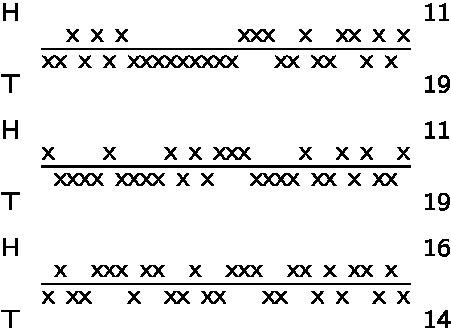
\includegraphics[width=0.8\linewidth]{fyz_fig077.pdf}
      \caption{Pozorované posloupnosti hlava znaků ve třech hrách po třiceti hodech 
              (\cite[s.~79]{Feynman01})}
      \label{fyz:fig077}
    \end{figure}
    Ve třech pokusech jsme ani jednou nedostali \num{15} hlav. Je to snad vinou mince? Nebo jsme se 
    zmýlili v úvaze vedoucí k závěru, že nejpravděpodobnější počet hlav v takové hře je \num{15}? 
    Abychom získali \num{100} experimentů, každý po \num{30} hodech, uskutečnili jsme dalších 
    \num{97} \uv{kol}. Výsledek experimentu ukazuje tab. \ref{fyz:fig079}\footnote{Po prvních třech 
    hrách jsme experiment ve skutečnosti provedli tak, že jsme silně zatřásli krabicí, v níž bylo 
    \num{30} mincí a pak jsme spočetli všechny hlavy.}.
    
    Prohlédneme-li si čísla v tab. \ref{fyz:fig079}, zjistíme, že většina výsledků je blízko čísla 
    \num{15} v tom smyslu, že se nacházejí mezi čísly \num{12} a \num{18}. K získání lepšího citu 
    pro chápání detailů těchto výsledků je vhodné zakreslit graf \emph{rozložení} výsledků. Určíme 
    počet her, v nichž jsme získali \(k\) hlav a znázorníme si je pro každé \(k\). Takový graf je 
    znázorněn na obr. \ref{fyz:fig078}. \num{15} hlav jsme získali ve \num{13} hrách. \num{14} 
    hlav jsme získali \num{13}-krát. \num{16} i \num{17} hlav jsme získali dokonce více než 
    \num{13}-krát.

    \begin{figure}[ht!]  %\ref{fyz:fig079}
      \centering
      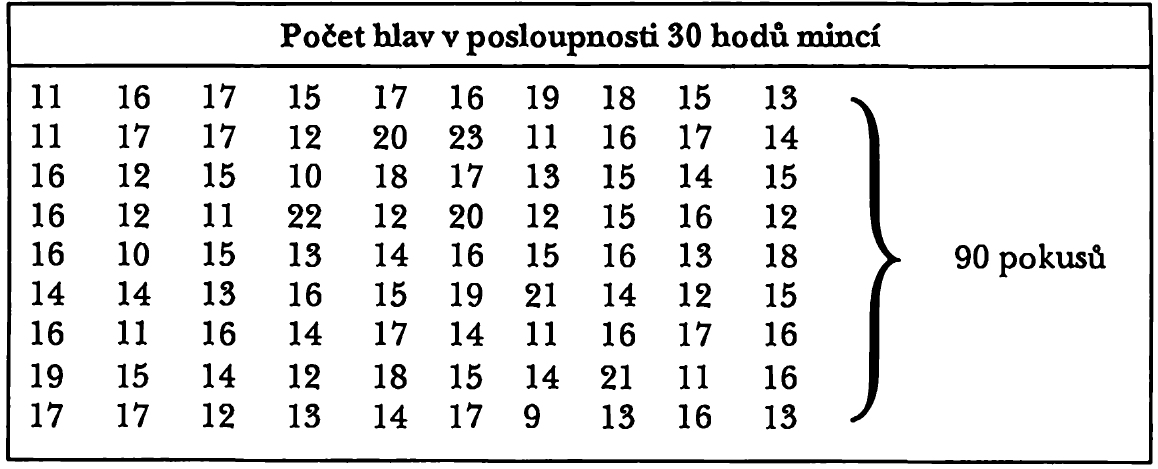
\includegraphics[width=1\linewidth]{fyz_fig079.png}
      \caption{Tabulka počtu hlav v posloupnosti \num{30} hodů mincí (\cite[s.~80]{Feynman01})}
      \label{fyz:fig079}
    \end{figure}
    Je možné z toho odvodit, že jde o jakousi zaujatost ve prospěch hlav? Nebyl náš „nejlepší 
    odhad“ dostatečně dobrý? Můžeme říci, že nejpravděpodobnější počet hlav pro jednu hru 
    sestávající z \num{30} hodů je \num{16}? Musíme být opatrní! Ve všech hrách se dohromady 
    uskutečnilo \num{3000} hodů. Hlav padlo celkem \num{1492}. Poměr počtu hlav k celkovému počtu 
    je tedy \num{0.497}, což je sice jen o málo, ale přece jen méně než polovina. Určitě tedy 
    nemůžeme předpokládat, že pravděpodobnost padnutí hlavy je větší než \num{0.5}! Skutečnost, že 
    v \emph{určité} sérii pozorování padne hlava nejčastěji \num{16}-krát, představuje 
    \emph{fluktuaci}. Jsme stále přesvědčeni, že \emph{nejpravděpodobnějším} počtem hlav je 
    \num{15}.
    
    Je možné položit otázku: Jaká pravděpodobnost, že hra s \num{30} hody dá \num{15}, \num{16} 
    nebo nějaký jiný počet hlav?“ Již jsme řekli, že při jednom hodu je pravděpodobnost pádu 
    \emph{jedné} hlavy \num{0.5} a i pravděpodobnost, že nepadne hlava, je \num{0.5}. Ve hře 
    sestávající ze dvou hodů máme \emph{čtyři} možné výsledky: \texttt{HH}, \texttt{HZ}, 
    \texttt{ZH}, \texttt{ZZ}. Protože každá z těchto posloupností je stejně pravděpodobná, můžeme 
    prohlásit, že
    \begin{enumerate}[noitemsep]
      \item pravděpodobnost padnutí dvou hlav je \num{1/4}, 
      \item pravděpodobnost padnutí jedné hlavy je \num{2/4}, 
      \item pravděpodobnost, že nepadne hlava je \num{1/4}. 
    \end{enumerate}
    Existují dva způsoby získávání jedné hlavy, ale jen jeden způsob získávání dvou hlav nebo žádné 
    hlavy.
    
    \begin{figure}[ht!]  %\ref{fyz:fig078}
      \centering
      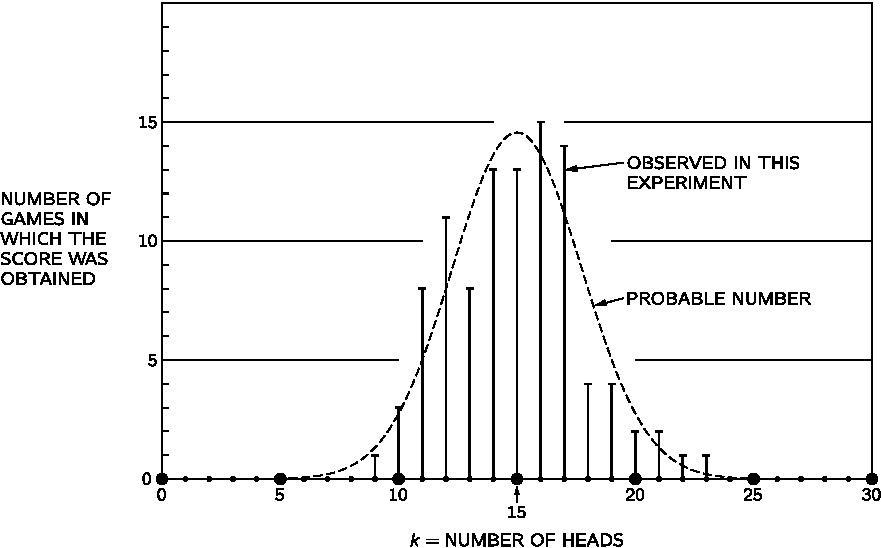
\includegraphics[width=1\linewidth]{fyz_fig078.pdf}
      \caption{Souhrn výsledků l00 her po 30pokusech. Vertikální čáry ukazuj počty her,v nichž 
              padlo \(k\) hlav. Přerušovaná čára ukazuje očekávaný počet her, v nichž padne \(k\) 
              hlav, získaný výpočtem pravděpodobnosti (\cite[s.~80]{Feynman01})}
      \label{fyz:fig078}
    \end{figure}
    
    Uvažujme nyní hru sestávající ze tří hodů. Pro třetí hod je stejně pravděpodobné, že padne 
    hlava nebo znak. Existuje jen jeden způsob získání tří hlav: v prvních dvou hodech 
    \emph{musely} padnout dvě hlavy a potom hlava i po třetím hodu. Existují však \emph{tři} 
    způsoby získání dvou hlav. Může padnout znak po padnutí dvou hlav (jeden způsob), nebo může 
    padnout hlava po padnutí jen jednoho znaku v prvních dvou hodech (dva způsoby). Tak pro možnosti
    \num{3}, \num{2}, \num{1}, \num{0} hlav existují \num{1}, \num{3}, \num{3}, \num{1} stejně 
    pravděpodobné způsoby představující celkově \num{8} různých posloupností. Příslušné 
    pravděpodobnosti jsou \num{1/8}, \num{3/8}, \num{3/8}, \num{1/8}.

    \begin{figure}[ht!]  %\ref{fyz:fig081}
      \centering
      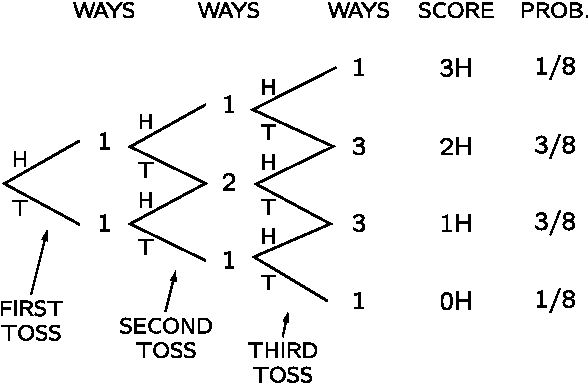
\includegraphics[width=1\linewidth]{fyz_fig081.pdf}
      \caption{Diagram znázorňující počet různých způsobů padnutí \num{0}, \num{1}, \num{2} nebo 
              \num{3} hlav ve hře sestávající ze tří hodů (\cite[s.~81]{Feynman01})}
      \label{fyz:fig081}
    \end{figure}
    
    To, co jsme řekli, je možno vyjádřit diagramem na obr. \ref{fyz:fig081}. Je jasné, že takové 
    diagramy lze sestrojit i pro hry s vyšším počtem hodů. Obr. \ref{fyz:fig080} znázorňuje takový 
    diagram pro hru se šesti hody. Počet způsobů odpovídajících libovolnému bodu diagramu je 
    vlastně počet různých cest (posloupností hlav a znaků), po nichž lze vyjít z počátečního bodu. 
    Počet úseků šikmo vzhůru udává počet vržených hlav. Soubor čísel, které se objevují v takovém 
    diagramu, je znám jako \textbf{Pascalův trojúhelník}. Čísla jsou známá i pod názvem 
    \emph{binomické koeficienty}, neboť se objevují i v rozvoji \((a + b)^n\). Označíme-li počet 
    hodů \(n\) a počet vržených hlav \(k\), pak se čísla vystupující v diagramu označují symbolem  
    \(\binom{n}{k}\). Bude vhodné připomenout, že binomické koeficienty 
    lze vypočítat ze vztahu
    \begin{equation}\label{fyz:eq074}
      \binom{n}{k} = \frac{n!}{k!(n-k)!}.
    \end{equation}
    kde \(n!\), nazývaný „n-faktoriál“, představuje součin \(n(n- 1)(n-2)\cdots (3)(2)(1)\).
    
    \begin{figure}[ht!]  %\ref{fyz:fig080}
      \centering
      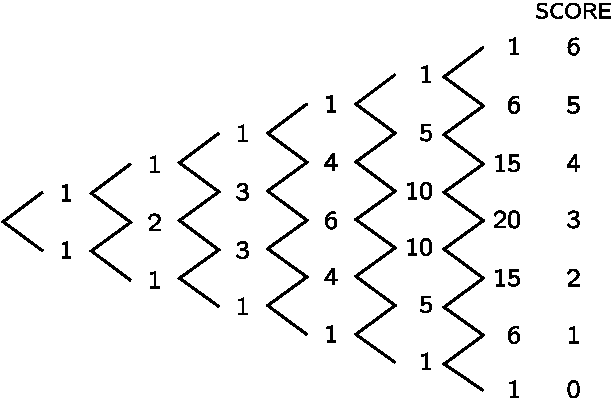
\includegraphics[width=1\linewidth]{fyz_fig080.pdf}
      \caption{Diagram jako na obr. \ref{fyz:fig081}, ale pro hru sestávající ze \num{6} hodů
               (\cite[s.~82]{Feynman01})}
      \label{fyz:fig080}
    \end{figure}
    
    Nyní již můžeme počítat pravděpodobnosti \(P(k, n)\) toho, že při \(n\) hodech padne hlava,
    pomocí definice (\ref{fyz:eq069}). Celkový počet možných posloupností je \(2^n\) (neboť každý
    hod připouští 2 výsledky) a počet způsobů získání \(k\) hlav je \(\binom{n}{k}\), přičemž
    všechny jsou stejně pravděpodobné. Proto máme
    \begin{equation}\label{fyz:eq075}
      P(k,n) = 
      \frac{\binom{n}{k}}{2^n}.
    \end{equation}
    
    Protože \(P(k, n)\) je podíl her, při nichž očekáváme, že padne \(k\) hlav, lze pak očekávat, 
    že při \num{100} hrách padne \(k\) hlav \(100\cdot P(k, n)\) krát. Přerušovaná čára na obr. 
    \ref{fyz:fig078} prochází body vypočítanými ze vztahu \(100\cdot P(k, 30)\). Vidíme, že padnutí 
    \num{15} hlav jsme \emph{očekávali ve} \num{14} nebo \num{15} hrách, zatímco tato událost byla 
    pozorována ve \num{13} hrách. Padnutí \num{16} hlav jsme \emph{očekávali ve} \num{13} nebo 
    \num{14} hrách, ale \num{16} hlav padlo v \num{16} hrách. Takové fluktuace jsou „součástí hry“.
    
    Použitou metodu je možné aplikovat i na tu nejobecnější situaci, v níž jsou jen dva možné 
    výsledky jednoho pozorování. Označme tyto dva výsledky \(V\) („výhra“) a \(P\) („prohra“). V 
    obecném případě pravděpodobnosti výsledku \(V\) nebo \(P\) u jedné události nemusí být stejné. 
    Označme \(p\) pravděpodobnost výhry \(V\). Potom \(q\), pravděpodobnost prohry, musí být nutně 
    \((1 - p)\). V souboru \(n\) pokusů je pravděpodobnost \(P(k, n)\) toho, že vyhrajeme 
    \(k\)-krát rovna
    \begin{equation}\label{fyz:eq076}
      \boxed{P(k,n) = \binom{n}{k}p^kq^{n-k}}\,.
    \end{equation}
    Tato pravděpodobnostní funkce se nazývá \textbf{Bernoulliho} nebo i \textbf{binomickou 
    pravděpodobností}.
    
  \section{Náhodná procházka}
    Existuje další zajímavý problém, v němž vystupuje myšlenka pravděpodobnosti. Je to problém 
    \emph{„náhodné procházky“}. Jako nejjednodušší verzi této úlohy si představme „hru“, v níž 
    „hráč“ startuje v bodě \(x = 0\) a při každém tahu má udělat krok \emph{buď} dopředu (směrem 
    \(k + x\)) nebo dozadu (směrem \(k - x\)). Volba se má uskutečnit náhodně, například pomocí 
    hodu mincí. Jak popíšeme výsledný pohyb? Ve své obecné formě se problém vztahuje na pohyb atomů 
    (nebo jiných částic) v plynech - jde o \textbf{Brownův pohyb} - a i na kombinaci chyb při 
    měřeních. Uvidíme, že problém náhodné procházky úzce souvisí s problémem házení mincí, o němž 
    jsme již hovořili.

    \begin{figure}[ht!]  %\ref{fyz:fig082}
      \centering
      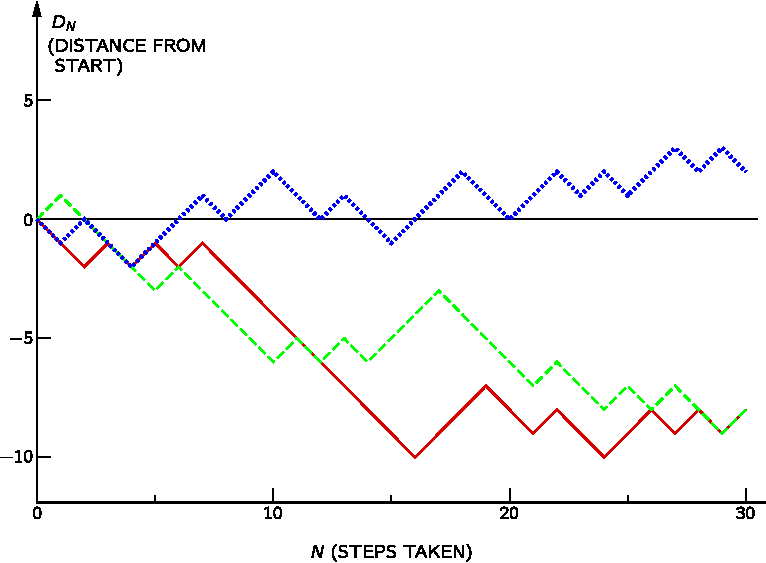
\includegraphics[width=1\linewidth]{fyz_fig082.pdf}
      \caption{Postup náhodné procházky. Horizontální souřadnice \(N\) představuje celkový počet 
               kroků: vertikální souřadnice \(D(N)\) představuje vzdálenost, do níž se chodec 
               dostal z počátečního bodu. (\cite[s.~83]{Feynman01})}
      \label{fyz:fig082}
    \end{figure}
    
    Nejprve si všimněme několika příkladů náhodné procházky. Postup chodce můžeme charakterizovat 
    čistou vzdáleností \(D_N\) ušlou v \(N\) krocích. Na obr. \ref{fyz:fig082} jsou vidět tři 
    příklady dráhy náhodného chodce. (Jako náhodné posloupnosti volby kroků jsme použili výsledky 
    házení mincí z obr. \ref{fyz:fig077}.)
    
    Co je možné říci o takovém pohybu? Především se můžeme ptát: Jak daleko se chodec v průměru 
    dostane?“ Musíme \emph{očekávat}, že jeho průměrný postup bude nulový, protože se stejně 
    pravděpodobně dostává dopředu nebo dozadu. Máme však takový pocit, že čím více \(N\) roste, tím 
    je pravděpodobnější, že chodec zabloudí dále od počátku. Proto se můžeme ptát, jaká je jeho 
    průměrná ušlá vzdálenost v \emph{absolutní hodnotě}, tj. jaký je průměr z \(\abs{D}\). Je však 
    výhodnější pracovat s jinou mírou „postupu“, se čtvercem vzdálenosti: \(D^2\) je kladné pro 
    kladný i záporný pohyb, a je proto vhodnou \emph{mírou} takového náhodného putování.
    
    Je možné dokázat, že očekávaná hodnota \(D_N^2\) je právě \(N\), tedy počet absolvovaných 
    kroků. „Očekávanou hodnotou“ rozumíme pravděpodobnou hodnotu (náš nejlepší odhad), kterou 
    můžeme považovat za \emph{očekávané} průměrné chování v mnoha opakovaných posloupnostech. 
    Takovou očekávanou hodnotu označujeme i \(\left\langle D_N^2\right\rangle\) a nazýváme ji i 
    \textbf{střední hodnotou čtverce vzdálenosti}. Po jednom kroku je \(D^2\) určitě rovno \(+1\), 
    máme tedy určitě \(\left\langle D_1^2\right\rangle = 1\). (Všechny vzdálenosti budou měřeny 
    tak, aby krok představoval jednotku. Jednotky vzdálenosti už nebudeme psát).

    Očekávanou hodnotu  \(\left\langle D_N^2\right\rangle\) pro \(N>1\) lze získat z \(D_{N-1}\). 
    Jestliže po \(N - 1\) krocích máme \(D_{N-1}\), pak po \(N\) krocích máme \(D_N = D_{N-1} + 1\) 
    nebo \(D_N = D_{N-1} - 1\). Pro druhé mocniny platí
    
    \begin{equation}\label{fyz:eq077}
      D_N^2 = 
        \begin{cases}
          D^2_{N-1} + 2D_{N-1} + 1 \\
          \quad\text{nebo}        \\
          D^2_{N-1} - 2D_{N-1} + 1
        \end{cases}
    \end{equation}
    Máme-li řadu nezávislých posloupností, očekáváme, že každá z těchto hodnot se objeví v polovině 
    případů, tedy naše průměrné očekávání je právě průměr ze dvou možných hodnot. Očekávaná hodnota 
    \(D_N\) je tedy \(D^2_{N-1} + 1\). Obecně můžeme očekávat pro \(D^2_{N-1}\) „očekávanou 
    hodnotu“  \(\left\langle D_{N-1}^2\right\rangle\) (podle definice !). Proto máme
    \begin{equation}\label{fyz:eq078}
      \left\langle D_N^2\right\rangle = \left\langle D_{N-1}^2\right\rangle + 1.
    \end{equation}
    Již jsme viděli, že \(\left\langle D_1^2\right\rangle = 1\) a proto musí být
    \begin{equation}\label{fyz:eq079}
      \left\langle D_N^2\right\rangle = N.
    \end{equation}
    Dostali jsme tedy velmi jednoduchý výsledek!
    
    Kdybychom při náhodné procházce chtěli „postup od začátku“ charakterizovat vzdáleností a ne 
    čtvercem vzdálenosti, museli bychom použít „střední kvadratickou vzdálenost“ \(D_{\text{stř}}\)
    \begin{equation}\label{fyz:eq080}
      D_{\text{stř}} = \sqrt{\left\langle D^2\right\rangle} = \sqrt{N}.
    \end{equation}
    
    Již jsme řekli, že náhodná procházka je z matematického hlediska velmi podobná hře házení 
    mincí, kterou jsme uvažovali na začátku kapitoly. Uvědomíme-li si, že směr každého kroku je v 
    souladu s padnutím hlavy nebo znaku ve hře s mincí, pak \(D\) je právě \(N_H - N_Z\), tedy 
    rozdíl počtu hlav a znaků. Protože je \(N_H + N_Z = N,\) kde \(N\) je celkový počet kroků (a 
    tedy i hodů), pak máme \(D = 2 N_H - N\). Již dříve jsme odvodili výraz pro očekávané rozdělení 
    \(N_H\) (nazývané i \(k\)) a dostali jsme výsledek (\ref{fyz:eq075}). Protože \(N\) je 
    konstanta, máme vlastně rozdělení odpovídající \(D\). (Protože pro každou hlavu navíc proti 
    \(N/2\) „chybí“ znak, máme faktor \(2\) mezi \(N_H\) a \(D\)). Grafy na obr. \ref{fyz:fig078} 
    představují rozdělení vzdáleností, jichž můžeme dosáhnout třiceti náhodnými kroky (kde \(k = 
    15\) znamená \(D = 0\), \(k= 16\), \(D = 2\) atd.).
    
    Odchylka \(N_H\) od očekávané hodnoty \(N/2\) je
    \begin{equation}\label{fyz:eq081}
      N_H - \frac{N}{2} = \frac{D}{2}
    \end{equation}
    a dále pro střední kvadratickou odchylku máme
    \begin{equation}\label{fyz:eq082}
      \left(N_H - \frac{N}{2}\right)_\text{stř} = \frac{1}{2}\sqrt{N}.
    \end{equation}
    
    V souladu s výsledky, které jsme získali pro \(D_{\text{stř}}\), očekáváme, že „typická“ 
    vzdálenost při třiceti krocích by měla být \(\sqrt{30} = \num{5.5}\), tedy typické \(k\) by 
    mělo být přibližně \(\num{5.5}/2 = \num{2.8}\) jednotek z \num{15}. Vidíme, že „šířka“ křivky 
    na obr. \ref{fyz:fig078} měřená od středu je přibližně \num{3} jednotky, což souhlasí s tímto 
    výsledkem.
    
    Dostali jsme se už tak daleko, že se můžeme zabývat otázkou, které jsme se dosud vyhýbali. Jak 
    můžeme rozhodnout, je-li mince „poctivá“ nebo „falešná“? Nyní můžeme na tuto otázku odpovědět 
    alespoň částečně. V případě poctivé mince očekáváme, že hlava se objeví v polovině případů, tj.
    \begin{equation}\label{fyz:eq083}
      \frac{\left\langle N_H\right\rangle}{N} = \num{0.5}.
    \end{equation}
    Očekáváme také, že skutečné \(N_H\) se bude lišit od \(N/2\) přibližně o \(\sqrt{N/2}\), nebo, 
    že podíl se bude lišit o
    \begin{equation}\label{fyz:eq084}
      \frac{1}{N}\cdot\frac{\sqrt{N}}{2} = \frac{1}{2\sqrt{N}}.
    \end{equation}
    Čím je \(N\) větší, tím blíže k jedné polovině bude podle našeho očekávání podíl \(N_H/N\).
    
    Na obr. \ref{fyz:fig083} je vynesen podíl \(N_H/N\) pro výše uvedenou hru s mincí. Z obrázku je 
    zřejmá snaha tohoto podílu dosáhnout hodnoty \num{0.5} při velkých \(N\). Naneštěstí pro žádnou 
    konkrétní hru nebo kombinaci her neexistuje \emph{záruka}, že pozorovaná odchylka bude alespoň 
    \emph{blízko očekávané odchylky}. Vždy existuje konečná možnost, že velká fluktuace - dlouhá 
    řada hlav nebo znaků způsobí libovolně velkou odchylku. Můžeme říci jen to, že v případě 
    odchylky, která se jen málo liší od hodnoty \(1/2\sqrt{N}\) (řekněme v rozsahu faktoru \num{2} 
    nebo \num{3}), nemáme důvod podezřívat minci z nepoctivosti. Je-li odchylka mnohem větší, může 
    vzniknout nedokazatelné podezření, že mince je upravena (nebo že hráč je příliš šikovný!).
    
    \begin{figure}[ht!]  %\ref{fyz:fig083}
      \centering
      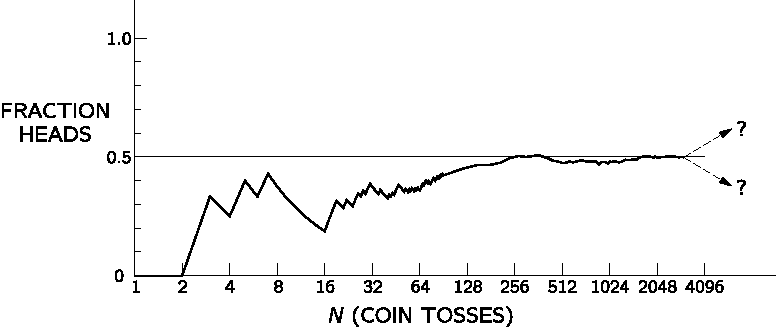
\includegraphics[width=1\linewidth]{fyz_fig083.pdf}
      \caption{Podíl hodů, v nichž padla hlava v určité posloupnosti \(N\) hodů mincí  
               (\cite[s.~85]{Feynman01})}
      \label{fyz:fig083}
    \end{figure}
    
    Nehovořili jsme ani o tom, co dělat v tom případě, kdy máme vážný důvod předpokládat, že 
    „mince“ nebo podobný jiný „náhodně“ se chovající předmět (například plochý kámen, který může 
    dopadnout jen na jednu nebo druhou stranu) \emph{budou mít} různé pravděpodobnosti, že padne 
    hlava nebo znak. Definovali jsme \(P(H) =\left\langle N_H\right\rangle/N\). Jak se dozvíme, co 
    je možné \emph{očekávat} pro \(N_H\). To nejlepší, co je možné v některých případech udělat, je 
    pozorovat počty hlav, které padnou při velkém počtu hodů. Z nedostatku lepší možnosti, musíme 
    položit \(\left\langle N_H\right\rangle = N_H\) (pozorované). (Co jiného je možné očekávat?) 
    Musíme si však uvědomit, že v takovém případě různé experimenty nebo různí pozorovatelé mohou 
    stanovit jinou hodnotu \(P(H)\). Je však možné \emph{očekávat}, že tyto hodnoty by se měly 
    lišit nejvýše odchylkou \(1/2\sqrt{N_H}\), je-li \(P(H)\) blízko \num{0.5}. Experimentální 
    fyzik říká, že „experimentálně určená“ pravděpodobnost má „chybu“ a píše
    \begin{equation}\label{fyz:eq085}
      P(H) = \frac{N_H}{N}\pm\frac{1}{2\sqrt{N}}.
    \end{equation}
    
    U takového výrazu se předpokládá, že \emph{existuje} „pravdivá“ nebo „správná“ pravděpodobnost, 
    kterou by bylo možné vypočítat, kdybychom toho dost věděli, a že pozorování mohou být zatížena 
    „chybou“ následkem fluktuace. Takovýto předpoklad však není možné logicky zdůvodnit. Je snad 
    lepší si uvědomit, že pojem pravděpodobnosti je svým způsobem subjektivní, že je vždy založen 
    na nejistých poznatcích a že jeho kvantitativní vyjádření podléhá změnám při získávání dalších 
    informací.
        
  \section{Rozložení pravděpodobnosti}
    Vraťme se opět k náhodné procházce a uvažujme o její obměně. Předpokládejme, že kromě náhodné 
    volby \emph{směru} (+ nebo -) každého kroku se mění i \emph{délka} kroku nějakým 
    nepředvídatelným způsobem, přičemž jedinou podmínkou je to, že v \emph{průměru} je délka kroku 
    jednotková. Takovýto případ lépe vystihuje něco takového, jako je tepelný pohyb molekul v 
    plynu. Je-li \(S\) délka kroku, pak \(S\) může dosáhnout jakékoli hodnoty, ale nejčastěji bude 
    \uv{blízko} \num{1}. Konkrétně budiž \(\left\langle S^2\right\rangle = 1\), nebo, což je totéž 
    \(S_{\text{stř}} = 1\). Při odvozování \(\left\langle D^2\right\rangle\) budeme postupovat jako 
    předtím, s tím rozdílem, že rovnice (\ref{fyz:eq078}) se nyní změní na
    \begin{equation}\label{fyz:eq086}
      \left\langle D_N^2\right\rangle 
        = \left\langle D_{N-1}^2\right\rangle + \left\langle s^2\right\rangle
        = \left\langle D_{N-1}^2\right\rangle + 1.
    \end{equation}
    Stejně jako předtím, i nyní dostaneme
    \begin{equation}\label{fyz:eq087}
      \left\langle D_N^2\right\rangle = N.
    \end{equation}
    Jaké bude nyní rozložení vzdáleností \(D\). Jaká je například pravděpodobnost toho, že \(D = 
    0\) po \num{30} krocích? Taková pravděpodobnost je nulová! Pravděpodobnost, že \(D\) bude 
    \emph{libovolná daná} hodnota, je nulová, neboť je zcela nepravděpodobné, že by součet všech 
    zpětných kroků (různých délek) byl přesně stejný jako součet kroků vpřed. Nemůžeme sestrojit 
    takový graf jako na obr. \ref{fyz:fig078}.
    
    Podobné znázornění jako na obr. \ref{fyz:fig078} je však možné, neptáme-li se na 
    pravděpodobnost \(D\) rovného přesně \num{0.1} nebo \num{2}, ale jestliže se zajímáme o 
    pravděpodobnost \(D\) \emph{v blízkosti} \num{0.1} nebo \num{2}. Definujme \(P(x, \Delta x)\) 
    jako pravděpodobnost toho, že \(D\) bude ležet v intervalu šířky \(\Delta x\) v okolí bodu 
    \(x\) (například od \(x\) po \(x + \Delta x\)). Očekáváme, že pro malé \(\Delta x\) je 
    pravděpodobnost toho, že \(D\) bude ležet v tomto intervalu, úměrná \(\Delta x\), tj. šířce 
    intervalu. Můžeme proto psát
    \begin{equation}\label{fyz:eq088}
      P(x,\Delta x) = p(x)\Delta x.
    \end{equation}
    Funkci \(p(x)\) nazýváme \textbf{hustotou pravděpodobnosti}.
    
    Tvar \(p(x)\) závisí na počtu kroků \(N\) i na rozdělení jednotlivých délek kroků. Nemůžeme to 
    zde dokazovat, ale pro velké \(N\) je hustota \(p(x)\) stejná pro všechna rozumná rozdělení 
    jednotlivých délek kroků a závisí jen na \(N\). Na obr. \ref{fyz:fig084} je znázorněno \(p(x)\) 
    pro tři hodnoty \(N\). Všimněte si, že pološířky těchto křivek (jejich rozšíření na úrovni 
    poloviny maximální výšky) jsou \(\sqrt{N})\) v souladu s našimi předcházejícími úvahami.
    
    Dále si můžeme všimnout, že hodnota \(p(x)\) v blízkosti nuly je nepřímo úměrná \(\sqrt{N}\). 
    Je tomu tak proto, že všechny křivky mají podobný tvar a plochy pod křivkami musí být stejné. 
    Protože \(p(x)\Delta x\) je pravděpodobnost nalezení \(D\) v \(\Delta x\) při malých hodnotách 
    \(\Delta x\), můžeme určit pravděpodobnost toho, že \(D\) se nachází někde uvnitř libovolného 
    intervalu ohraničeného body \(x_1\), \(x_2\) tak, že tento interval rozdělíme na malé části 
    \(\Delta x\) a vypočteme součet členů \(p(x)\Delta x\) pro každou takovou část.     
    Pravděpodobnost, že \(D\) se nachází někde mezi \(x_1\) a \(x_2\), což můžeme zapsat \(P(x_1 < 
    D < x_2)\), je rovna obsahu vyšrafované oblasti na obr. \ref{fyz:fig085}. Čím menší jsou 
    přírůstky \(\Delta x\), tím přesnější bude výsledek. Proto můžeme napsat, že
    \begin{equation}\label{fyz:eq089}
      P(x_1 < D < x_2) = \sum p(x)\Delta x = \int_{x_1}^{x_2}p(x)dx.
    \end{equation}
    Obsah plochy pod celou křivkou je pravděpodobnost, že \(D\) se někde nachází (tj. má nějakou 
    hodnotu mezi \(x=-\infty\) a  \(x= +\infty\)).

    \luagraphic[1]{fyz_fig084.pdf}{Hustota pravděpodobnosti dosažení vzdálenosti \(D\) od počátku
    při náhodné procházce sestávající z \(N\) kroků (\(D\) se měří v jednotkách střední kvadratické
    délky kroku) (\cite[s.~87]{Feynman01})}{fyz:fig084}
      
    Tato pravděpodobnost je rovna \(1\). Musí tedy být
    \begin{equation}\label{fyz:eq090}
      \int_{-\infty}^{\infty}p(x)dx = 1.
    \end{equation}
    
    Protože křivky na obr. \ref{fyz:fig084} se rozšiřují úměrně \(\sqrt{N}\), musí být jejich výška 
    úměrná \(1\sqrt{N}\), aby se zachoval celkový obsah plochy rovný \num{1}.

    \begin{figure}[ht!]  %\ref{fyz:fig084}
      \centering
      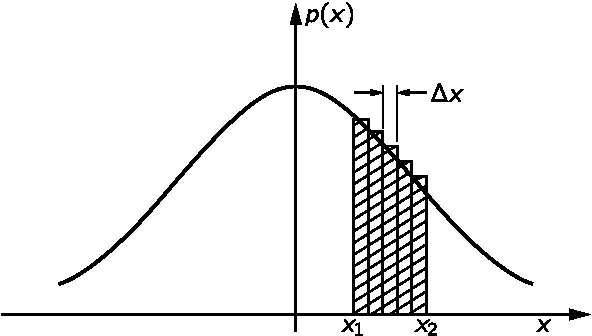
\includegraphics[width=1\linewidth]{fyz_fig085.pdf}
      \caption{Pravděpodobnost, že při náhodné procházce se ušlá vzdálenost \(D\) nachází mezi 
                body  \(x_1\) a \(x_2\), je dána obsahem plochy pod křivkou \(p(x)\) mezi \(x_1\) a 
                \(x_2\).
                \cite[s.~87]{Feynman01}}
       \label{fyz:fig085}
    \end{figure}
    
    S hustotou pravděpodobnosti, o níž jsme právě hovořili, se setkáváme nejčastěji. Je známá jako 
    \textbf{normální} nebo \textbf{Gaussova hustota pravděpodobnosti}. Její matematický zápis je
    \begin{equation}\label{fyz:eq091}
      p(x) = \frac{1}{\sigma\sqrt{2\pi}}e^{-\frac{x^2}{2\sigma^2}},	
    \end{equation}    
    přičemž veličina \(\sigma\) se nazývá \emph{standardní odchylkou}. V našem případě je \(\sigma 
    = \sqrt{N}\), nebo je-li střední kvadratická délka kroku různá od \num{1}, je 
    \(\sigma=\sqrt{N}S_\text{stř}\).
    
    Již jsme uvedli, že pohyb molekuly nebo každé jiné částice v plynu je podobný náhodné 
    procházce. Předpokládejme, že otevřeme láhev s organickou sloučeninou a necháme část její páry 
    uniknout do vzduchu. Existuje-li proudění vzduchu, tak že vzduch cirkuluje, budou unášeny i 
    uvedené páry. Jenže i v dokonale klidném vzduchu se budou páry postupně rozptylovat - 
    difundovat - dokud neproniknou do celé místnosti. Můžeme je registrovat podle jejich barvy nebo 
    zápachu. Jednotlivé molekuly organických par se šíří i v klidném vzduchu v důsledku 
    molekulárního pohybu způsobovaného srážkami s jinými molekulami. Známe-li délku „kroku“ a počet 
    kroků za sekundu, můžeme zjistit pravděpodobnost, v jaké vzdálenosti od svého původního místa 
    se ocitne po určitém čase jedna nebo několik molekul. Postupem času počet kroků roste a plyn se 
    rozplývá tak, jak je znázorněno křivkami na obr. \ref{fyz:fig084}. V jedné z dalších kapitol 
    určíme, jak závisí délka a frekvence kroků na teplotě a tlaku plynu.
    
    Již jsme hovořili o tom, že tak plynu je následkem srážek molekul se stěnami nádoby. Až později 
    přejdeme ke kvantitativnímu popisu tohoto jevu, musíme znát rychlost molekul narážejících na 
    stěnu, protože síla jejich nárazu závisí na rychlosti. Nemůžeme však hovořit o \emph{určité} 
    rychlosti molekul. Tento děj můžeme popsat jen pomocí pravděpodobností. Molekula může mít 
    jakoukoli rychlost, ale některé rychlosti jsou pravděpodobnější než jiné. Procesy probíhající v 
    plynu můžeme popsat pomocí pravděpodobnosti \(p(v)\Delta v\), že daná molekula má rychlost z 
    intervalu \(v, v+ \Delta v\). Hustota pravděpodobnosti \(p(v)\) je přitom funkcí rychlosti 
    \(v\). Později se dozvíte, jak Maxwell využitím zdravého rozumu a myšlenek teorie 
    pravděpodobnosti našel matematické vyjádření funkce \(p(v)\). Tvar\footnote{Maxwellův výraz je 
    \(p(v) = Cv^2e^{-av^2}\), kde \(a\) je konstanta související s teplotou a \(C\) je zvoleno tak, 
    aby celková pravděpodobnost byla rovna jedné.} funkce \(p(v)\) je znázorněn na obr. 
    \ref{fyz:fig086}. Rychlost může dosáhnout libovolné hodnoty, ale s největší pravděpodobností 
    bude blízká nejpravděpodobnější nebo očekávané hodnotě \(\langle v\rangle\)).
    
    \begin{figure}[ht!]  %\ref{fyz:fig086}
      \centering
      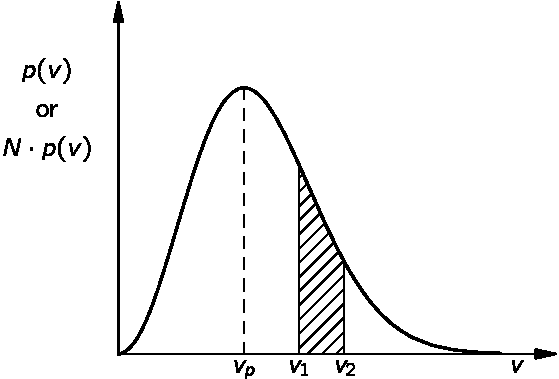
\includegraphics[width=1\linewidth]{fyz_fig086.pdf}
      \caption{Rozložení rychlosti molekul plynu  (\cite[s.~88]{Feynman01})}
      \label{fyz:fig086}
    \end{figure}
    
    O křivce znázorněné na obr, \ref{fyz:fig086} často uvažujeme trochu jinak. Máme-li molekuly 
    plynu uzavřené v typické nádobě (která má objem např. \SI{1}{\litre}), jde vlastně o velmi 
    velké množství \(N\) molekul (\(N\approx\num{e22}\)). Protože \(p(v)\Delta v\) je 
    pravděpodobnost toho, že \emph{jedna} molekula bude mít rychlost z intervalu \(\Delta v\), pak 
    podle naší definice pravděpodobnosti bude \emph{očekávaný} počet molekul \(\langle N\rangle\) s 
    rychlostmi z intervalu \(\Delta v\)
    \begin{equation}\label{fyz:eq092}
      \langle N\rangle = Np(v)\Delta v.
    \end{equation}
    Veličinu \(Np(v)\) proto nazýváme „\emph{rozdělením molekul podle rychlosti}“. Plocha pod 
    křivkou mezi dvěma hodnotami rychlosti \(v_1\) a \(v_2\), např. vyšrafovaná plocha na obr. 
    \ref{fyz:fig086}, představuje (v případě křivky \(Np(v)\)) očekávaný počet molekul s rychlostmi 
    mezi \(v_1\) a \(v_2\). Protože v případě plynu máme obvykle co činit s velkým počtem molekul, 
    předpokládáme malé odchylky od očekávaných hodnot (jako \(1/\sqrt{N}\)), a proto často 
    vynecháváme slovo „očekávaný“ a říkáme: „Počet molekul s rychlostmi mezi \(v_1\) a \(v_2\) 
    odpovídá obsahu příslušné plochy pod křivkou.“ Nesmíme však zapomenout, že takové výroky se 
    vždy týkají \emph{pravděpodobných} počtů.
    
  \section{Princip neurčitosti}
    Myšlenky pravděpodobnosti jsou jisté užitečné při popisu chování řádově \num{e22} molekul v 
    plynu, protože již samotný pokus o určení polohy nebo rychlosti každé molekuly by byl úžasně 
    nepraktický. Když se poprvé na takový problém aplikovala teorie pravděpodobnosti, chápalo se to 
    jako \emph{vhodný} způsob popisu tak složitých situací. Dnes jsme však toho názoru, že idea 
    pravděpodobnosti je při popisu atomových dějů \emph{nevyhnutelná}. Podle kvantové mechaniky, 
    matematické teorie částic, existuje vždy jistá nepřesnost při \emph{určení} poloh a rychlostí. 
    V nejlepším případě můžeme říci, že existuje jistá pravděpodobnost toho, že částice se bude 
    nacházet v blízkosti určitého bodu \(x\).
    
    Hustotu pravděpodobnosti \(p_1(x)\) udáme tak, že \(p_1(x)\Delta x\) představuje 
    pravděpodobnost výskytu částice mezi \(x\) a \(x+ \Delta x\). Je-li částice dostatečně dobře 
    lokalizovaná, např. v blízkosti \(x_1\), bude mít funkce \(p_1(x)\) průběh podobný grafu na 
    obr. \ref{fyz:fig087a}. Podobně musíme určit rychlost částice pomocí hustoty pravděpodobnosti 
    \(p_2(v)\), přičemž \(p_2(v)\Delta v\) je pravděpodobnost toho, že rychlost je v intervalu mezi 
    \(v\) a \(v+\Delta v\).
    
    \begin{figure}[ht!]  %\ref{fyz:fig087}
      \centering
      \subcaptionbox{\label{fyz:fig087a}}{\luafigure[0.70]{fyz_fig087a.pdf}}              \\
      \subcaptionbox{\label{fyz:fig087b}}{\luafigure[0.70]{fyz_fig087b.pdf}}
      \caption{Hustota pravděpodobnosti pozorování polohy a rychlosti částice  
               (\cite[s.~89]{Feynman01})}
      \label{fyz:fig087}
    \end{figure}
    
    Jeden ze základních výsledků kvantové mechaniky spočívá v tom, že funkce \(p_1(x)\) a 
    \(p_2(v)\) není možné vybrat nezávisle, zejména nemohou být obě dvě libovolně úzké. Označíme-li 
    charakteristickou „šířku“ křivky \(p_1(x)[\Delta x]\) a křivky \(p_2(v)\) zase \([\Delta v]\), 
    jak je ukázáno na obrázku, potom příroda vyžaduje, aby \emph{součin} těchto šířek nebyl menší 
    než číslo \(h/m\), kde \(m\) je hmotnost částice a \(h\) je základní fyzikální konstanta zvaná 
    \textbf{Planckova konstanta}. Tento základní vztah je možné zapsat ve tvaru
    \begin{equation}\label{fyz:eq093}
      [\Delta x][\Delta v]\geq\frac{h}{m}.
    \end{equation}
    Tato rovnice je matematickým vyjádřením \textbf{Heisenbergova principu neurčitosti}, o němž 
    jsme se již zmínili.
    
    Protože pravá strana rovnice (\ref{fyz:eq093}) je konstantní, pak, „přinutíme-li“ částici 
    zaujmout určité místo, skončí to tím, že velmi vzroste její rychlost. Nebo přinutíme-li částici 
    pohybovat se velmi pomalu, nebo velmi přesnou rychlostí, „rozplyne se“, takže nebudeme umět 
    říci, kde se přesně nachází. Částice se chovají velmi podivně!
    
    Princip neurčitosti vyjadřuje přirozenou nejasnost, která musí existovat při každém pokusu 
    popsat přírodu. Náš nejpřesnější popis přírody musí byt v řeči \emph{pravděpodobnosti}.Jsou 
    však lidé, kteří se neumějí smířit s takovýmto popisem přírody. Domnívají se, že kdybychom 
    věděli, co se s částicí  \emph{skutečně} děje, mohli bychom znát současně její přesnou rychlost 
    a polohu. Na začátku rozvoje kvantové mechaniky tento problém velmi znepokojoval Einsteina. 
    Často potřásal hlavou a říkal \uv{Vždyť bůh neháže kostkou, aby rozhodl, jak se má pohybovat 
    elektron!} Dlouho se trápil s tímto problémem a pravděpodobně se nikdy nesmířil se skutečnosti, 
    že je to ten nejlepší popis přírody, který dokážeme udělat. Několik málo fyziků se ještě stále 
    zabývá tímto problémem doufajíce, že svět je možné popsat nějak jinak a vyloučit neurčitost v 
    chování částic. Zatím však v tomto směru nikdo nebyl úspěšný. 
    
    Nevyhnutelná neurčitost při určování polohy částice nabývá významu tehdy, když chceme popsat 
    strukturu atomů. V atomu vodíku, jenž má jádro skládající se z jednoho protonu a mimo jádro má 
    jeden elektron, je neurčitost v poloze elektronu tak velká jako atom samotný! Proto nemůžeme 
    dost dobře hovořit o elektronu pohybujícím se po určité dráze kolem protonu. Nanejvýš můžeme 
    říci, že existuje určitá pravděpodobnost \(p(r)\Delta V\) pozorování elektronu v elementu 
    objemu \(\Delta V\) ve vzdálenosti \(r\) od protonu. Hustota pravděpodobnosti \(p(r)\) udává 
    kvantová mechanika. Pro neporušený vodíkový atom je \(p(r) = Ae^{-\frac{r^2}{a^2}}\), což 
    představuje funkci se zvonovitým grafem podobnou funkci na obr. \ref{fyz:fig085}. Číslo \(a\) 
    představuje \uv{charakteristický} poloměr, za nímž funkce rychle klesá. Protože je malá 
    pravděpodobnost výskytu elektronu ve větších vzdálenostech od jádra než \(a\), můžeme \(a\) 
    považovat za \uv{poloměr atomu}, což je asi \num{e-10} metru. 

    \begin{figure}[ht!]  %\ref{fyz:fig088}
      \centering
      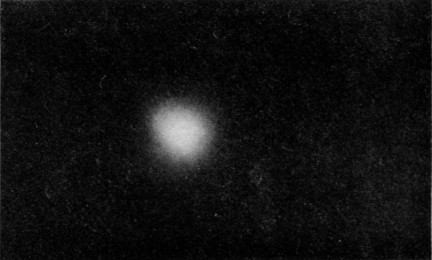
\includegraphics[width=0.8\linewidth]{fyz_fig088.jpg}
      \caption{Způsob znázornění atomu vodíku. Hustota (bělost) oblaku představuje hustotu 
               pravděpodobnosti výskytu elektronu. 
               (\cite[s.~90]{Feynman01})}
      \label{fyz:fig088}
    \end{figure}
    Představu o atomu vodíku můžeme získat, znázorníme-li si oblak, jehož hustota je úměrná hustotě 
    pravděpodobnosti výskytu elektronu. Příklad takového oblaku je na obr. \ref{fyz:fig088}. Naší 
    nejlepší \uv{představou} vodíkového atomu je tedy jádro obklopené \uv{elektronovým oblakem} (ve 
    skutečnosti však máme na mysli \uv{oblak pravděpdobnosti}). Elektron je někde tam, ale příroda 
    nám dovoluje poznat jen \emph{pravděpodobnost} jeho výskytu na určitém místě.
    
    Ve svém úsilí po co nejúplnějším poznání přírody dospěla moderní fyzika poznání, že jisté věci 
    není možné \uv{poznat} s jistotou. Mnohé z našich poznatků vždy zůstanou nejisté. Nanejvýš 
    můžeme znát jejich pravděpodobnosti. 
    
  \section{Příklady a cvičení}
  
%} %tikzset
%---------------------------------------------------------------------------------------------------
  % % !TeX program = lualatex
% !TeX root = luaking.tex
% !TeX encoding = UTF-8
% !TeX spellcheck = cs_CZ
%---------------------------------------------------------------------------------------------------
\graphicspath{{../src/MAI/img/}}
% file mai1ch04b.tex
%---------------------------------------------------------------------------------------------------
\setchaptertoc
\chapter{Náhodné veličiny}\label{mai:IchapIVb}
  \epigraph{\emph{The true logic of this world is in the calculus of probabilities.}}{James Clerk 
    Maxwell}
  \section{Úvod}\label{mai:IchapIVsecIII}
    Hodnota některých veličin je určena jednoznačně a „jednou provždy“. Kdykoli budeme její hodnotu 
    zjišťovat, tehdy dostaneme totéž - takže ji ani opakovaně zjišťovat nemusíme. Příkladem může 
    být skoro prázdná peněženka, ve které jsou třeba tři koruny. Dokud nebudeme pracovat a do 
    peněženky něco nepřidáme, bude hodnota veličiny \(X\) (počet korun v peněžence) stále rovna 
    \num{3}. Nemá smysl se do peněženky vůbec dívat. Pokud budeme do peněženky přidávat každý den 
    dvě koruny, také budeme vědět, jak se veličina \(X\) mění, aniž bychom se do peněženky dívali. 
    Po \(n\) dnech bude hodnota \(X = 3 + 2n\). Většina veličin, se kterými se setkáváme, se však 
    takto nechová. Jejich hodnoty se totiž často řídí náhodnými vlivy, takže při každém
    měření veličiny \(X\), tj. zjišťování její hodnoty, můžeme získat odlišný výsledek než při 
    měřeních předchozích. Uveďme některé příklady náhodných veličin.
    
    \begin{itemize}
      \item \textbf{Příklad s novorozenci}: Nechť jé veličinou \(X\) počet chlapců ve stovce 
            novorozených dětí. Zkušenost říká, že tento počet je v průměru o něco větší než 
            \num{50}, avšak pro různé skupiny po stovce novorozených dětí bude počet chlapců 
            kolísat. V jedné skupině bude \num{52}, v jiné \num{54}, někde třeba \num{60}, nebo 
            také \num{45}.
      \item \textbf{Příklad s meteoroidy a meteority}: Pro astronomy může být důležitou veličinou 
            \(X\) počet meteoroidů, které za rok dopadnou do zemské atmosféry. Jinou veličinou, 
            třeba \(K\), může být roční počet meteoritů, tj. těch meteoroidů, které v atmosféře 
            neshořely zcela, ale jejich část dopadla na povrch Země. Také tyto hodnoty budou pro 
            každý roční interval poněkud odlišné, neboť i počet dopadnuvších meteoroidů a 
            meteoritů podléhá vlivům, které se nedají přesně předvídat.
      \item \textbf{ Příklad s tlakoměrem}: Bude-li lékař měřit pacientovi tlak několikrát po 
            sobě, určitě také naměří několik různých hodnot. Krevní tlak je citlivý na náhodné 
            vlivy, třeba i na vnitřní rozrušení pacienta vyplývající ze strachu z bílého pláště.
      \item \textbf{Opakovaná měření fyzikální veličiny}: Chceme-li změřit třeba odpor elektrického
            vodiče (drátu), jedná se o měření nepřímé. Nemůžeme odpor změřit přímo, třeba jako      
            to můžeme udělat pro délku. Většinou měříme napětí \(U\) na vodiči a proud \(I\), který 
            jím protéká. Odpor pak zjišťujeme jako podíl \(R = U/I\). Změříme-li napětí i proud 
            jednou, dostaneme konkrétní hodnotu \(R\). Budeme-li měření napětí a proudu provádět 
            opakovaně, budeme dostávat poněkud odlišné hodnoty \(U\) a \(I\), a tedy i odlišné 
            hodnoty \(R\). Sledované veličiny se chovají jako náhodné. Je to způsobeno řadou 
            náhodných vlivů jak na veličiny samotné, tak na jejich měření (nepřesnost odečítání 
            údajů na stupnicích, apod.).
    \end{itemize}
  
    Při každém fyzikálním (a vlastně i nefyzikálním) experimentu máme co do činění s náhodnými 
    veličinami. Při chemických analýzách je náhodnou veličinou třeba koncentrace dané látky
    v roztoku, při experimentech biologických třeba počet uhynuvších rostlin ve stovce sazenic, 
    počet pozorovaných prvoků v zorném poli mikroskopu, výskyt vzácných ptáků ve sledované 
    lokalitě, apod. V následujících odstavcích definujeme náhodné veličiny přesněji a naučíme se s 
    nimi zacházet. Uvidíme, že zjištění určité hodnoty náhodné veličiny je otázkou jisté 
    pravděpodobnosti. Také lépe objasníme, co znamená vyjádření „v průměru“, které jsme občas v 
    předchozím textu použili a intuitivně mu jistě rozuměli.
  
    \subsection{Jak dobrý je to střelec - diskrétní rozdělení}
      Mimořádně vhodnou ukázkou náhodné veličiny je příklad se sportovním střelcem, kterým jsme
      uvedli celou kapitolu o pravděpodobnostech.
  
      %--Ještě jednou střelba, tentokrát přesněji---------------------
      % !TeX spellcheck = cs_CZ
\begin{mdframed}[style=mdexam]
  \begin{example}\label{mai:exam064}
    \textbf{Ještě jednou střelba, tentokrát přesněji}\newline
    Názvem pochopitelně nemyslíme přesnější střelbu, ale přesnější komentář, který již bude založen
    na našich znalostech o pravděpodobnosti. Dejme tomu, že podmínky střelby jsou pevně dány a
    nemění se. Patří k nim zcela jistě typ zbraně, typ terče, vzdálenost stanoviště střelce od
    terče, základní povětrnostní podmínky. Výsledky jsou pak závislé na zručnosti střelce, avšak
    jsou ovlivněny náhodným i vlivy (foukne nenadálý vítr, střelec se lekne, zatřese se mu ruka,
    náhodně se mírně pozmění vzdálenost ústí hlavně od terče nebo její sklon, apod.). Počty
    dosažených bodů daného střelce při jednom výstřelu, nebo při sérii deseti výstřelů, atd., jsou
    tedy náhodnými veličinami. Pokusme se posoudit zručnost střelce přesněji. Označme jako náhodnou
    veličinu \(X\) počet bodů dosažených při jednom výstřelu. Nejprve určeme, jakých hodnot může
    nabývat. Všichni víme, jak vypadá běžný střelecký terč. Aby však naše počty nebyly příliš
    komplikované a zdlouhavé, uvažujme o terči mnohem jednodušším. Bude tvořen vnitřním černým
    kruhem s hodnotou \(3\) body, dále středním šedivým mezikružím s hodnotou \(2\) body a vnějším
    bílým mezikružím s hodnotou \(1\) bod. Střelba do terče mimo vnější kružnici nebo zcela mimo
    terč představuje bodovou hodnotu \(0\). Při jednom výstřelu tedy může střelec docílit v principu
    jakékoli z možných hodnot

    {\centering
      \captionsetup{type=figure}
      \luafigure[0.6]{mai_fig070.pdf}
      \captionof{figure}{Ilustrace k příkladu \ref{mai:exam064}}
      \label{mai:fig070}
    \par}
    \vspace{0.5em}
    \begin{equation*}
      X\in\{x_1, x_2, x_3,x_4\} = \{0,1,2,3\}.
    \end{equation*}
    Informace, jakých hodnot může náhodná veličina nabývat, je jistě nejen cenná, ale je pro
    jakékoli další úvahy nezbytná. Sama o sobě je však nepostačující. O střelcově zručnosti se na
    základě konstrukce terče nic nedovídáme. Kvalitativně jinou informaci získáme, víme-li, že
    možných hodnot zásahu dociluje střelec s následujícími pravděpodobnostmi:

    {\centering
      \begin{tabular}{c|rrrr}
        \(x_i\)    &      0     &      1     &      2     &      3       \\
        \hline
        \(p_i\)    & \num{0.03} & \num{0.28} & \num{0.52} & \num{0.17} 
      \end{tabular}
    \par}

    Můžeme tak třeba zjistit, kolika bodů střelec zhruba docílí s vysokou pravděpodobností při pěti
    výstřelech. Tento počet je
    \begin{gather*}
      5\cdot(\num{0.03}\cdot0 + \num{0.28}\cdot1 + \num{0.52}\cdot2 + \num{0.17}\cdot3) = 
      5\cdot\num{1.83} = \num{9.15} \simeq 9.
    \end{gather*}
    Pro každou pětici výstřelů může být počet dosažených bodů samozřejmě poněkud odlišný. Veličina
    \(Y\) představující počet dosažených bodů na pět výstřelů je rovněž veličinou náhodnou. Je nám
    však jasné, že hodnota dosažených bodů v každé pětici výstřelů je s vysokou pravděpodobností
    blízká číslu 9. Co to znamená „s vysokou pravděpodobností“? Dokážeme ji spočítat? Pokusme se o
    to. Především bychom museli určit, o kolik bodů se smí dosažený počet lišit od hodnoty 9,
    abychom jej ještě považovali za „blízký číslu 9“ . Tato volba závisí čistě na naší vůli a bude
    jí odpovídat i vypočtená pravděpodobnost. Dejme tomu, že zvolíme tento interval od 7 do 11 bodů
    včetně. Jev, jehož pravděpodobnost hledáme, je tedy
    \begin{itemize}
      \item \(A\) : Při pěti výstřelech získá střelec \num{7} nebo \num{8} nebo \num{9} nebo \num{10} 
            nebo \num{11} bodů.
      \item[] Jevy
      \item \(A_j\) : Střelec získá při pěti výstřelech \(j\) bodů.
    \end{itemize}
    jsou po dvou neslučitelné, pravděpodobnost jevu \(A\) tedy bude rovna součtu pravděpodobností
    \begin{equation*}
      p(A) = \sum_{j=7}^{11} p(A_j).
    \end{equation*}
   
    Pozor! Pravděpodobnosti \(p(Aj)\) jsou odlišné od pravděpodobností zadaných v první tabulce. Ta
    se totiž týká pěti výstřelů, zatímco tabulka \ref{mai:tab004} je pro jeden výstřel. Musíme tedy
    určit pravděpodobnosti \(p(A_j)\). K tomu je třeba zjistit všechny možnosti, jak docílit součtu
    bodů \(j\) pomocí pěti sčítanců nabývajících hodnot \num{0} až \num{3}. Soupis je v následující
    tabulce. Tabulka uvádí různé rozklady součtu na sčítance, počet případů, jak se tento rozklad
    realizuje (různé pořadí dosažených bodů při jednotlivých výstřelech) a pravděpodobnosti
    jednotlivých rozkladů zaokrouhlené na tři platná místa.

    Jak jsme spočítali pravděpodobnosti jednotlivých rozkladů? Dejme tomu, že počet bodů dosažených
    při pěti výstřelech je \(j\). Nechť \(j = j_1 + j_2 + j_3 + j_4 + j_5\) je rozklad hodnoty \(j\)
    na součet pěti sčítanců. Čísla \(j_1\) až \(j_5\) se pohybují od \num{0} do \num{3}, mohou být i
    shodná. Například jeden z možných rozkladů bodového součtu \(j = 9\) je \(9 = 3 + 2 + 2 + 1 +
    1\). Pravděpodobnost, že při pěti nezávislých výstřelech budou jednotlivé zásahy činit \(j_1\),
    \(j_2\), \(j_3\) , \(j_4\)a \(j_5\) bodů, je
    \begin{equation*}
      p_{j1}p_{j2}p_{j3}p_{j4}p_{j5}.
    \end{equation*}
    Pro případ zvoleného konkrétního rozkladu čísla \num{9} je to \(p_3p_2^2p_1^2\) - Zásahy s
    bodovým ziskem \(j_1\) až \(j_5\) mohou být realizovány v různých pořadích (například \(\num{3}
    + \num{2} + \num{2} + \num{1} + \num{1} = \num{2} + \num{3} + \num{2} + \num{1} + \num{1}
    =\ldots\), atd.). Označme počet všech takových pořadí \(n_{j_1\ldots j_5}\). (Pro \(j = \num{3}
    + \num{2} + \num{2} + \num{1} + \num{1}\) je \(n_{32211} = \binom{5}{2}\binom{3}{2} = 30\): Dvě
    z pěti pozic pro umístění dvou dvojek lze vybrat \(\binom{5}{2}\) způsoby, ze zbývajících tří
    pozic lze dvě pro umístění jedniček vybrat \(\binom{3}{2}\) způsoby a na trojku zbude poslední
    pozice.) Pravděpodobnost \(p_{j_1\ldots j_5}\) daného rozkladu čísla \(s\) pak je
    \begin{equation*}
      p_{j_1\ldots j_5} = n_{j_1\ldots j_5}p_{j_1}p_{j_2}p_{j_3}p_{j_4}p_{j_5}
    \end{equation*}

    {\centering
    \resizebox{1\textwidth}{!}{%
    \begin{tabular}{c|rrrr}
      součet \(j\)& sčítance   &    počet   & ppst rozkladu & \(p(A_j)\) \\ \hline
            7     & 3+3+1+0+0  & \num{30}   & \num{2.18e-4} & \num{0.102} \\
                  & 3+2+2+0+0  & \num{30}   & \num{1.24e-3} & \\
                  & 3+2+1+1+0  & \num{60}   & \num{1.25e-2} & \\
                  & 3+1+1+1+1  & \num{5}    & \num{5.22e-3} & \\
                  & 2+2+2+1+0  & \num{20}   & \num{2.36e-2} & \\
                  & 2+2+1+1+1  & \num{10}   & \num{5.94e-2} & \\ \hline
            8     & 3+3+2+0+0  & \num{30}   & \num{4.06e-4} & \num{0.185} \\
                  & 3+3+1+1+0  & \num{30}   & \num{2.04e-3} & \\
                  & 3+2+2+1+0  & \num{60}   & \num{2.32e-2} & \\
                  & 3+2+1+1+1  & \num{20}   & \num{3.88e-2} & \\
                  & 2+2+2+2+0  & \num{5}    & \num{1.10e-2} & \\
                  & 2+2+2+1+1  & \num{10}   & \num{1.10e-1} & \\ \hline
            9     & 3+3+3+0+0  & \num{10}   & \num{4.42e-5} & \num{0.238} \\
                  & 3+3+2+1+0  & \num{60}   & \num{7.57e-3} & \\
                  & 3+3+1+1+1  & \num{10}   & \num{6.34e-3} & \\
                  & 3+2+2+2+0  & \num{20}   & \num{1.43e-2} & \\
                  & 3+2+2+1+1  & \num{30}   & \num{1.08e-1} & \\
                  & 2+2+2+2+1  & \num{5}    & \num{1.02e-1} & \\ \hline
          10      & 3+3+3+1+0  & \num{20}   & \num{8.25e-4} & \num{0.215} \\
                  & 3+3+2+2+0  & \num{30}   & \num{7.03e-3} & \\
                  & 3+3+2+1+1  & \num{30}   & \num{3.53e-2} & \\
                  & 3+2+2+2+1  & \num{20}   & \num{1.34e-1} & \\
                  & 2+2+2+2+2  & \num{1}    & \num{3.80e-2} & \\ \hline
          11      & 3+3+3+2+0  & \num{20}   & \num{1.53e-3} & \num{0.133} \\
                  & 3+3+3+1+1  & \num{10}   & \num{3.85e-3} & \\
                  & 3+3+2+2+1  & \num{30}   & \num{6.56e-2} & \\
                  & 3+2+2+2+2  & \num{5}    & \num{6.21e-2} & \\ \hline
    \end{tabular}}
    \captionsetup{type=table} 
    \captionof{table}{Tabulka rozkladů pro daný součet bodů: ve sloupci \uv{počet} je uveden počet 
                      kombinací, které vedou ke stejnému nástřelu (sloupec \uv{součet}) a s daným
                      bodovým ohodnocením (sloupec \uv{sčítanec})}
    \label{mai:tab004}
    \par}
    \vspace{\baselineskip}

    Pro rozklad \(\num{9} = \num{3} + \num{2} + \num{2} + \num{1} + \num{1}\) je (výsledek viz také
    v tabulce)
    \begin{equation*}
      p_{32211} =30\cdot p_3p_2^2p_1^2 = \num{30}\cdot\num{0.17}\cdot\num{0.52}^2\cdot\num{0,282} 
                \simeq \num{0.108}.
    \end{equation*}
    Pravděpodobnost \(p(A_j)\) je součtem pravděpodobností jednotlivých rozkladů čísla \(j\).
    Konečně pravděpodobnost, že střelec dosáhne bodového výsledku \(y \in [7, 11]\), je rovna součtu
    pravděpodobností \(p(A_j)\) pro \(j = 7, 8, 9, 10, 11\). Tato hodnota je \num{0.873}, tedy
    opravdu poměrně vysoká, jak jsme očekávali. Také bychom mohli říci, že střelec dosahuje při
    každé pětici výstřelů „v průměru“ \num{9} bodů, a tedy při jednom výstřelu „v průměru“ \num{1.8}
    bodů. Pokud bychom „průměrnou hodnotu“ jednoho výstřelu počítali i pro jiný počet výstřelů než
    pro pět, budeme dostávat čísla, která budou hodnotě \num{1.8} velmi blízká.
  \end{example}
\end{mdframed}
      %---------------------------------------------------------------
    
    Položme si ještě otázku, jak můžeme zjistit pravděpodobnosti, se kterými střelec dosáhne při
    jednom výstřelu daného počtu bodů. Prakticky to lze provést jedině tak, že střelec mnohokrát
    vystřelí na terč a jeho zásahy budou při tom zaznamenávány. Dejme tomu, že vystřelil \(n\)-krát 
    a že počet výstřelů, při nichž byl bodový zisk \(j\) bodů ( \(j = 0, 1, 2, 3\)), byl \(n_j\). 
    Pak pro pravděpodobnost bodového zisku \(j\) bodů při jednom výstřelu je \(p_j = n_j/n\). 
    Kdybychom provedli skutečný experiment se střelcem a počítali pravděpodobnosti \(p_j\) znovu a 
    znovu po každém dalším výstřelu, viděli bychom, že pro malé hodnoty \(n\) nejprve kolísají a 
    pro rostoucí \(n\) se začínají ustalovat a již kolísají velmi málo. Tímto postupem bychom je 
    mohli určit tak, aby byly pro náš účel rozumně přesné - třeba s přesností na dvě platná místa. 
    Rozumnou přesností je zde myšlena skutečnost, že nemá smysl chtít zjišťovat pravděpodobnost 
    třeba na šest platných míst. Vzhledem k principiální přítomnosti náhodných vlivů se kolísání 
    pravděpodobností nikdy nezbavíme, takže platná místa na pozicích, kde se kolísání trvale 
    projevuje již bez ohledu na zvyšující se \(n\), nemají smysl.
    
    V příkladu \ref{mai:exam064} jsme se již velmi těsně přiblížili důležitým charakteristikám, 
    které určují náhodnou veličinu a jsou přitom matematicky korektně definovány. Viděli jsme, že 
    známe-li jen hodnoty, kterých může náhodná veličina nabývat, nemůžeme o ní říci již nic 
    dalšího. Známe-li však ještě pravděpodobnosti, se kterými jednotlivých hodnot nabývá, můžeme o 
    ní získat již velmi mnoho informací.

    \begin{mdframed}[style=highlight]
      \textbf{Náhodnou veličinou s diskrétním rozdělením} nazýváme takovou veličinu \(X\), která
      může nabývat konečně mnoha různých hodnot \((x_1, x_2, \ldots, x_k)\) s pravděpodobnostní
      \((p_1, p_2, \ldots, p_k)\) popřípadě spočetně mnoha hodnot \((x_1, x_2, \ldots)\) s 
      pravděpodobnostmi \((p_1, p_2, \ldots)\).
    \end{mdframed}

    Jevy \(A_j\) \uv{veličina \(X\) nabývá hodnoty \(x_j\)}, jsou po dvou neslučitelné. Platí
    \begin{equation*}
      \sum_{j=1}^{k}p_j = 1, \qquad\text{resp.}\qquad \sum_{j=1}^{k=\infty}p_j = 1
    \end{equation*}
    Pokud jde o druhý z obou případů, nebudeme se jím prozatím zabývat. Soubor všech dvojic
    \begin{equation*}
      \left\lbrace(x_j, p_j)\right\rbrace,\qquad j = 1, 2, \ldots, k,
    \end{equation*}
    se nazývá \textbf{rozdělení} náhodné veličiny \(X\). Můžeme je znázornit i graficky.

    %--Bernoulliovo (binomické) rozdělení---------------------------
    % !TeX spellcheck = cs_CZ
\begin{mdframed}[style=mdexam]
  \begin{example}\label{mai:exam065}
    \textbf{Bernoulliovo (binomické) rozdělení}\newline
    Představme si opět Bernoulliův pokus o \(n\) opakováních a pravděpodobností zdaru při jednom
    opakování rovnou \(p\) (kapitola \ref{mai:IchapIVsecIIssecIV}). Náhodnou veličinu \(X\)
    definujme jako počet zdarů při tomto pokusu. Tato veličina nabývá všech celočíselných hodnot
    \(x_j = j, 0 \leq j \leq n\), přitom hodnoty \(j\) nabývá s pravděpodobností určenou vztahem
    (\ref{mai:eq055}), v němž za \(x\) dosadíme \(j\). 
    
    {\centering
      \captionsetup{type=figure}
      \luafigure[1]{mai_fig044.pdf}
      \captionof{figure}{Bernoulliovo rozdělení
      \cite[s.~229]{Musilova2009MA1}
      \label{mai:fig044}}
    \par}
    
    Získané rozdělení je tedy
    \begin{equation*}
      \lbrace j,p_j\rbrace, \quad\text{kde}\quad p_j = \binom{n}{j}p^j(1 - p)^{n-j}.
    \end{equation*}
    Graf Bernoulliova rozdělení, které je často nazýváno také binomickým, je na obrázku 
    \ref{mai:fig044} pro \(n = 15\) a \(p = 1/2\) (červený asterisk).
    
    Z grafu je názorně vidět, co to znamená, že některé hodnoty veličiny \(X\) jsou více a jiné méně 
    pravděpodobné. Hodnota \(x_i\), veličiny \(X\), které odpovídá největší pravděpodobnost \(p_i\), 
    se nazývá nejpravděpodobnější hodnota. V případě Bernoulliova rozdělení na obrázku 
    \ref{mai:fig044} jsou takové hodnoty dvě, konkrétně \(x_7 = 7\) a \(x_8 = 8\).
    
      \begin{lstlisting}[style=luaCPPStyle, caption={PPST001.m}]
        citatel= factorial(n);
        jmenovatel= factorial(n-j).*factorial(j);
        binom = citatel./jmenovatel;
        f = binom.*p.^j.*(1-p).^(n-j);
      \end{lstlisting}
  \end{example}
\end{mdframed}
    %---------------------------------------------------------------
    
    Nyní definujeme další charakteristiky náhodné veličiny. Těmi základními jsou, kromě již 
    definované \emph{nejpravděpodobnější hodnoty}, ještě \textbf{střední hodnota}, \textbf{rozptyl} 
    (popřípadě jeho odmocnina, zvaná \textbf{střední kvadratická} nebo \textbf{směrodatná 
    odchylka}), \textbf{medián}, popřípadě \textbf{P-kvantil}. Pojem střední hodnoty jsme již v 
    podstatě vybudovali v příkladu se střelcem. Nyní postup zobecníme. Předpokládejme, že při 
    velkém počtu \(n\) měření náhodné veličiny \(X\) naměříme různé hodnoty \((x_1, x_2, \ldots, 
    x_k)\) tak, že hodnota \(x_1\) byla naměřena \(n_1\)-krát, hodnota \(x_2\) \(n_2\)-krát, atd., 
    až hodnota \(x_k\) \(n_k\)-krát. Je zřejmé, že součet četností \(n_1\), \(n_2\), až \(n_k\) 
    jednotlivých hodnot musí být roven celkovému počtu měření \(n\) a že podíly
    \begin{equation*}
      p_1 = \dfrac{n_1}{n}, \qquad p_2 = \dfrac{n_2}{n}, \qquad \ldots, \qquad p_k = \dfrac{n_k}{n},
    \end{equation*}
    představují pravděpodobnosti jednotlivých hodnot veličiny \(X\). Tím je zadáno její rozdělení,
    které ji plně charakterizuje. Položme si však otázku, zda by se veličina \(X\) přece jen nedala
    charakterizovat jedinou hodnotou, která by všechny různě pravděpodobné hodnoty v jistém
    smyslu „zastupovala“. Kdybychom třeba takto měřili délku stolu, jistě bychom na otázku „Kolik
    měří stůl?“ neodpovídali tím, že bychom tazateli předložili získané rozdělení, i když by taková
    odpověď byla nejvýstižnější. Určitě bychom uvedli jedinou hodnotu. Ale jakou? I laika napadne,
    že by takovou reprezentativní hodnotou mohl být aritmetický průměr naměřených hodnot \(x_1\) až
    \(x_k\). Bylo by ale správné vzít jen prostý aritmetický průměr těchto různých hodnot a nebrat 
    ohled na skutečnost, že některé byly naměřeny s větší a jiné s menší četností? Nikoliv. 
    Reprezentativní hodnota veličiny \(X\) nemá zastupovat jen naměřené hodnoty, ale celé 
    rozdělení. Určitá hodnota \(x_j\) bude mít tím větší vliv na reprezentativní hodnotu, s čím 
    větší četností byla naměřena. Protože byla naměřena \(n_j\)-krát, musíme ji také tolikrát do 
    aritmetického průměru započíst.Získáváme tak \textbf{vážený aritmetický průměr} naměřených 
    hodnot, neboli \emph{střední hodnotu}
    
    \begin{mdframed}[style=highlight]
      \begin{align}\label{mai:eq059}
        \left\langle x \right\rangle 
          &= \dfrac{n_1x_1 + n_2x_2 + \cdots + n_kx_k}{n}  \nonumber \\
          &= p_1x_1 + p_2x_2 + \cdots + p_kx_k             \nonumber \\
          &= \sum_{j=1}^{k}p_jx_j.
      \end{align}
    \end{mdframed}
    Součet všech pravděpodobností \(p_1 + p_2 + \cdots + p_k\) je pochopitelně \textbf{roven jedné}.

    %--Střední hodnota Bernoulliova rozdělení-----------------------
    % !TeX spellcheck = cs_CZ
\begin{mdframed}[style=mdexam]
  \begin{example}\label{mai:exam066}
    \textbf{Bernoulliovo (binomické) rozdělení}\newline
    Pro střední hodnotu Bernoulliova rozdělení platí
    \begin{equation*}
      \langle j \rangle = \sum_{j=0}^{n}j\cdot p_j
        = \sum_{j=1}^{n}j\begin{pmatrix} n \\ j \end{pmatrix}p^j(1-p)^{n-j} = np.
    \end{equation*}
    
    Tento vztah lze dokázat matematickou indukcí vzhledem k proměnné \(n\). Na tomto místě nebudeme
    důkaz provádět pro jeho poměrnou zdlouhavost. Každý jej však může zvládnout. Vzpomeňme si v tuto
    chvíli na náš chybný intuitivní odhad v kapitole \ref{mai:IchapIVsecIIssecIV}, v níž jsme
    poprvé hovořili o Bernoulliově pokusu v souvislosti s hody mincí. Chybně jsme tam odhadli
    pravděpodobnost, že při \(n\) opakováních pokusu nastane v polovině z nich zdar. Tato chyba
    vznikla v důsledku naší zkušenosti, že když budeme mincí vícekrát házet, padne hlava (zdar)
    skutečně zhruba v polovině případů. Vidíme nyní, že \(n/2\) reprezentuje střední hodnotu náhodné
    veličiny \(X =\) \textbf{počet zdarů při \(n\) hodech mincí}. A to naší zkušenosti již odpovídá.
  \end{example}
\end{mdframed}
    %---------------------------------------------------------------
    
    Posuďme nyní situaci, kdy náhodná veličina \(Y\) je funkcí náhodné veličiny \(X, Y = f(X)\).
    V takovém případě má rozdělení veličiny \(Y\) tvar
    \begin{equation*}
      \left\lbrace (f(x_j), p_j)\right\rbrace, \qquad j = 1, 2, \ldots, k.
    \end{equation*}
    Pravděpodobnost hodnoty \(f(x_j)\) je stejná jako pravděpodobnost hodnoty \(x_j\). Pro výpočet
    střední hodnoty veličiny \(Y\) pak platí
    \begin{equation}\label{mai:eq060}
      \left\langle y \right\rangle = \sum_{j=1}^{k}f(x_j)p_j.
    \end{equation}
    (V obecnější situaci může být náhodná veličina \(Y\) funkcí několika náhodných veličin \(X_1\), 
    \(X_2\), až \(X_s\)).
    
    Může vzniknout oprávněná otázka, zda při výpočtu \(\left\langle y \right\rangle\), popřípadě 
    dalších charakteristik veličiny \(Y\), nevznikne nějaký problém, nebude-li funkce \(f(X)\) 
    prostá. V takovém případě by totiž některé hodnoty veličiny \(Y\) splynuly i pro různá \(x_j\). 
    Například pro \(Y = f(X) = X^2\) by pro hodnoty \(x_r\) a \(x_s\) vázané vztahem \(x_r = -x_s\) 
    (pokud by veličina \(X\) směla takových hodnot nabývat) platilo \(y_{rs} = y_r = y_s\). 
    Pravděpodobnost této společné hodnoty by pak přece byla \((p_r + p_s)\). Tato úvaha je 
    samozřejmě správná, avšak ve výpočtu střední hodnoty veličiny Y
    podle vztahu (\ref{mai:eq060}) je již obsažena. Do součtu totiž vstupují sčítance \(y_rp_r\) i 
    \(y_sp_s\), jejichž součet je při rovnosti \(y_r = y_s\) roven \(y_{rs}(p_r +p_s)\) Společná 
    hodnota \(y_{rs}\) je tedy započtena se správnou vahou.
    
    Uvažujme nyní o tom, jak „směrodatná“, tj. do jaké míry opravdu „reprezentativní“, je
    střední hodnota náhodné veličiny. Intuitivně cítíme, že střední hodnota bude reprezentovat
    rozdělení náhodné veličiny tím lépe, čím méně se od ní budou jednotlivé hodnoty odchylovat na 
    obě strany. Význam slova „odchylovat“ musíme ovšem nějak kvantitativně zachytit.
    \emph{Odchylkou} hodnoty \(x_j\) veličiny \(X\) od střední hodnoty \(\left\langle x 
    \right\rangle\) budeme celkem přirozeně rozumět rozdíl \((x_j - \langle x\rangle)\). Vzniká tak 
    náhodná veličina \(\Sigma = X - \langle x \rangle\) s rozdělením \(\{(x_j - \langle x\rangle, 
    p_j)\}\), \(j = 1, 2, \ldots, k\) . Bude tou správnou charakteristikou odchýlení hodnot 
    veličiny \(X\) od střední hodnoty střední hodnota \(\langle\sigma\rangle\)? Vypočtěme ji 
    (odhadněte předem, co asi tak vyjde):
    \begin{align*}
      \langle\sigma\rangle 
          &= \sum_{j=1}^{k}(x_j - \langle x\rangle)p_j
           = \sum_{j=1}^{k}x_jp_j - \langle x\rangle\sum_{j=1}^{k}p_j   \\
          &= \langle x\rangle - \langle x\rangle = 0.
    \end{align*}
    Čekali jste to? Nepochybně ano. Veličina \(X - \langle x\rangle\) nedává tedy žádný obraz o 
    tom, jak jsou hodnoty \(x_j\) „rozptýleny“ okolo střední hodnoty \(\langle x\rangle\). Kladné 
    odchylky jsou to tiž kompenzovány těmi zápornými. Aby k takové kompenzaci nedošlo, stačí vzít 
    v úvahu absolutní hodnotu veličiny \(\Sigma\), popřípadě její kvadrát. Vezměme v úvahu druhý z 
    obou námětů a vypočtěme \(\langle \sigma^2\rangle\), takzvaný \textbf{rozptyl veličiny} \(X\):
    \begin{align}\label{mai:eq061}
       D(X) &= \langle \sigma\rangle = \sum_{j=1}^{k}(x_j - \langle x\rangle)^2p_j    \nonumber \\
            &= \sum_{j=1}^{k}x_j^2p_j - 2\langle x\rangle\sum_{j=1}^{k}x_jp_j 
              + \langle x\rangle^2\sum_{j=1}^{k}p_j                                   \nonumber \\
            &= \langle x^2\rangle - 2\langle x\rangle^2 + \langle x\rangle^2          \nonumber \\
            &= \langle x^2\rangle - \langle x\rangle^2.
    \end{align}
    hodnota
    \begin{mdframed}[style=highlight]
      \begin{equation}\label{mai:eq062}
        \sigma(x) = \sqrt{\langle \sigma^2\rangle} = \sqrt{\langle x^2\rangle - \langle x\rangle^2}
      \end{equation}
    \end{mdframed}
    se nazývá \textbf{směrodatná odchylka} (v některých terminologiích též \emph{střední 
    kvadratická odchylka}) veličiny \(X\). Podíl \(\sigma(x)/ \langle x\rangle\) se nazývá 
    \textbf{relativní směrodatná odchylka} (v některé terminologii též \emph{variační koeficient}).

    \begin{mdframed}[style=highlight]
      Důležitým pojmem je \textbf{distribuční funkce}. Je to funkce \(F\) jedné reálné proměnné 
      \(x\) definovaná ve vztahu k náhodné veličině \(X\) takto: Předpokládejme, že hodnoty \(x_1\)
      až \(x_k\), jichž může náhodná veličina \(X\) nabývat, jsou seřazeny vzestupně, tj. \(x_1 <
      < x_2 < \ldots < x_k\). Pak
      \begin{equation}\label{mai:eq063}
        F: \realset\ni x\longleftrightarrow 
        F(x) = \sum_{\mathclap{\substack{j=1\\ x_s \leq x \leq x_{s+1}}}}^{s}p_j
      \end{equation}
    \end{mdframed}

    Přestože je veličina \(X\) diskrétní, je distribuční funkce funkcí spojité proměnné. Její 
    funkční hodnoty se však mění skokem. Vidíme to z následující tabulky a z grafu na obrázku 
    \ref{mai:fig045}, v němž je distribuční funkce znázorněna pro případ střelby (příklad 
    \ref{mai:exam064})

    \begin{table}[ht!]
      \centering
      \begin{tabular}{c|c}
        \textbf{interval}                 &  \textbf{distribuční funkce}             \\ \hline
            \(-\infty, x_1\)              &    \(F(x) = 0\)                         \\
            \(\left[x_1, x_2\right)\)     &    \(F(x) = p_1\)                       \\
            \(\left[x_2, x_3\right)\)     &    \(F(x) = p_1 + p_2\)                 \\
                    \(\ldots\)            &       \(\ldots\)                         \\
            \(\left[x_j, x_{j+1}\right)\) &    \(F(x) = p_1 + p_2 + \cdots + p_j\)  \\
                   \(\ldots\)             &       \(\ldots\)                         \\
            \(\left[x_k, \infty\right)\)  &    \(F(x) = p_1 + \cdots + p_k =1\)     \\ \hline
            \end{tabular}
      % \caption{ }
    \end{table}

    \luagraphic[1]{mai_fig045.pdf}{Distribuční funkce k příkladu \ref{mai:exam064}. 
    \cite[s.~233]{Musilova2009MA1}}{mai:fig045}

    Zadáním distribuční funkce je naopak jednoznačně určeno rozdělení veličiny \(X\). Pro jednotlivé
    pravděpodobnosti totiž platí
    \begin{equation*}
      p_j = F(x_j) - F(x_{j-1})\;\text{pro}\; 2\leq j \leq k, \; p_1 = F(x_1).
    \end{equation*}
    
    Hledejme nyní hodnotu \(\overline{x}_P\) definovanou tak, že pravděpodobnost, že při náhodném 
    opakování pokusu nabude veličina \(X\) kterékoli z přípustných hodnot \(x_j \leq 
    \overline{x}_p\), je rovna \(P\). Znamená to, že pro \(x = \overline{x}_P\) má distribuční 
    funkce nabýt předepsané hodnoty \(P\). Abychom \(\overline{x}_P\), takzvaný 
    \(P\)\textbf{-kvantil}, určili, řešíme rovnici
    \begin{equation}\label{mai:eq064}
      \sum_{j=1}^{s}p_j = P
    \end{equation}
    vzhledem k neznámému počtu sčítanců \(s\). V případě veličiny s diskrétním rozdělením se ovšem
    může stát, že pro nevhodně zvolenou hodnotu \(P\) nebude mít rovnice řešení. To proto, že 
    veličina \(X\) může nabývat jen hodnot, které lze očíslovat přirozenými čísly, takže při každé 
    změně horní meze sumy \(s\) o jedničku se suma mění skokem. Vidíme to jak v předcházející 
    tabulce, tak v grafu na obrázku \ref{mai:fig045}. Pro \(P = \num{0.5}\) se \(P\)-kvantil 
    \(\overline{x}_p\), pokud je vůbec definován, nazývá \textbf{medián}. Značí se pouze 
    \(\overline{x}\).

    %--Ještě střelba------------------------------------------------
    % !TeX spellcheck = cs_CZ
\begin{mdframed}[style=mdexam]
  \begin{example}\label{mai:exam067}
    \textbf{Ještě střelba}\newline
    Problém s definici \(P\)-kvantilu u veličiny s diskrétním rozdělením snadno vidíme na příkladu
    střelby (příklad \ref{mai:exam064}). Pro \(s\) postupně 1, 2, 3, 4 nabývá součet na levé straně
    rovnice (\ref{mai:eq064}) hodnot
    
    \begin{equation*}
      p_1 = \num{0.003},\; p_1 + p_2 = \num{0.31},\; p_1 + p_2 + p_3 = \num{0.83}, 
    \end{equation*}
    \begin{equation*}
      p_1 + p_2 + p_3 + p_4 = 1.
    \end{equation*}
    Pojem \(P\)-kvantil je tedy definován jen pro \(P = 0\), \(P = \num{0.03}\), \(P = \num{0.31}\),
    \(P = \num{0.83}\) a \(P = 1\). (Pro \(P = 0\) a \(P = 1\) nemá žádný praktický význam.)
    Nenabývá-li \(P\) žádné z přípustných hodnot, tj. některé hodnoty z množiny \(\{\num{0.03},
    \num{0.31}, \num{0.83}, 1\}\), nemá rovnice pro s řešení a \(P\)-kvantil není vůbec definován.
    Je-li hodnotou \(P\) některý prvek této množiny, dostaneme z rovnice (\ref{mai:eq064}) sice
    jediné řešení \(s\), avšak která hodnota bude \(P\)-kvantilem? Z grafu je vidět, že pro každou
    přípustnou hodnotu \(P\) vyhovuje podmínce celý interval proměnné \(x\). Konkrétní výsledky
    shrnuje následující tabulka:
    
    {\centering
      \begin{tabular}{c|@{\hspace{3pt}}c@{\hspace{3pt}}c@{\hspace{3pt}}c@{\hspace{3pt}}c@{\hspace{3pt}}c}
        \(P\) & \num{0} & \num{0.03} & \num{0.31} & \num{0.83} & \num{1} \\ \hline
        \(F(x) = P\) & \((-\infty,\num{0})\) & \(\left[0, 1\right)\) &
        \(\left[1, 2\right)\) & \(\left[2, 3\right)\) & \(\left[3, \infty\right)\)
      \end{tabular}
    \par}
    
    Význam pojmu \(P\)-kvantil je tedy pro náhodnou veličinu s diskrétním rozdělením poněkud sporný.
    Uplatní se však velmi dobře u veličin s rozdělením spojitým, jak uvidíme později. Než však
    opustíme příklad se střelbou definitivně, spočtěme si ještě střední hodnotu a rozptyl veličiny
    \(X\), kterou jsme definovali jako počet dosažených bodů při jednom výstřelu:
    \begin{align*}
      \langle x \rangle 
          &= \sum_{j=1}^{4}x_jp_j                                                                \\
          &= 0\cdot\num{0.03} + 1\cdot\num{0.28}+ 2\cdot\num{0.52} + 3\cdot\num{0.17} = \num{1.83}, 
    \end{align*}
    \begin{align*}
      D(X)  &= \sum_{j=1}^{4}\left(x_j - \langle x \rangle \right)^2p_j                          \\
            &= (0-\num{1.83})^2\cdot\num{0.03}+(1-\num{1.83})^2\cdot\num{0.28}                   \\
            &+ (2-\num{1.83})^2\cdot\num{0.52}+(3-\num{1.83})^2\cdot\num{0.17}                   \\
                &\simeq\num{0.541},                                                              \\
      \sigma(x) &\simeq\num{0.736}.
    \end{align*}

    V příkladu \ref{mai:exam064} jsme odhadovali, kolika bodů dosáhne střelec při pěti výstřelech.
    Tato hodnota nám vyšla \(\num{5}\cdot\num{1.83} = \num{9.15} = 9\). Nyní vidíme je jí souvislost
    se střední hodnotou náhodné veličiny \(X\). Pokud totiž definujeme veličinu \(Y\) jako počet
    bodů dosažených při pěti výstřelech, je \(Y = 5X\) a \(\langle y \rangle = 5\langle x \rangle\).
    Uvažujme nyní o významu směrodatné odchylky. Zřejmě \(\sigma(y) = 5\sigma(x) = \num{3.68}\).
    Směrodatná odchylka \(\sigma(y)\) určuje interval \((\langle y \rangle - \sigma(y), \langle y
    \rangle + \sigma(y)) = (\num{5.32}, \num{12.68})\). Možnosti bodového zisku ležící v tomto
    intervalu jsou \num{6} až \num{12} bodů včetně. Pokud bychom doplnili tabulku z příkladu
    \ref{mai:exam064} ještě o rozklady a jejich pravděpodobnosti pro bodový součet při pěti
    výstřelech \(j = \num{6}\) a \(j = \num{12}\), dostaneme \(p(A_6) = \num{0.0400}\), \(p(A_{12})
    = \num{0.0550}\). Pravděpodobnost, že výsledek střelce leží při pěti výstřelech v intervalu
    \((\langle y \rangle - \sigma(y), \langle y \rangle + \sigma(y)) = (\num{5.32}, \num{12.68})\),
    je tedy
    \begin{align*}
      \sum_{j=6}^{12}p(A_j) &= p(A_6) + \sum_{j=7}^{11}p(A_j) + p(A_{12})                \\
                            &= \num{0.0400} + \num{0.873} + \num{0.0550} \simeq \num{0.97}.
    \end{align*}
    Při výpočtu jsme využili výsledku z příkladu \ref{mai:exam064}, kde jsme počítali
    pravděpodobnost, že střelec dosáhne bodového výsledku v rozmezí \num{7} až \num{11} bodů.
    Směrodatná odchylka \(\sigma(y)\) veličiny \(Y\) určuje tedy v tomto případě interval okolo
    střední hodnoty \(\langle y \rangle\), v němž leží střelcův bodový zisk s velmi vysokou
    pravděpodobností \SI{97}{\percent}. Tento výsledek lze velmi názorně interpretovat také takto:
    Vystřelí-li střelec pětkrát na terč, bude téměř s jistotou jeho bodový zisk ležet v intervalu
    určeném směrodatnou odchylkou, tj. bude ležet mezi šesti a dvanácti body. Není vyloučeno, že
    bodový zisk bude třeba pět bodů, nebo i nula, nebo naopak dokonce maximálních možných patnáct
    bodů. Všechny ty to možnosti dohromady jsou však vysoce nepravděpodobné, připadá na ně
    pravděpodobnost pouhé \SI{3}{\percent}!. Anebo ještě trochu jinak: Kdyby střelec při tréninku
    uskutečnil třeba sto sérií po pěti výstřelech, pak by skoro jistě bylo sedmadevadesát z nich v
    rozmezí bodového zisku \num{6} až \num{12} bodů a tři mimo. Toto konstatování ovšem opět
    nevylučuje možnost, že v rozmezí \num{6} až \num{12} bodů bude ležet jiný počet sérií než
    \num{97}. Může dokonce v principu dojít k tomu, že do této kategorie padnou série všechny nebo
    žádná. Takový výsledek je však opět vysoce nepravděpodobný.
    
    Není vyloučeno, že i po prostudování tohoto příkladu bude někdo stále nespokojen s tím, že je
    naše vyjadřování „málo přesné“. Vzhledem k pravděpodobnostnímu charakteru posuzovaných jevů
    však, bohužel, přesnější být nemůže.
  \end{example}
\end{mdframed}
    %---------------------------------------------------------------
    
    Příklad \ref{mai:exam067} názorně vypovídá o významu směrodatné odchylky. Viděli jsme, že 
    intervalu o šířce \(2\sigma(y)\) s hodnotou \(\langle y \rangle\) uprostřed odpovídá vysoká 
    pravděpodobnost, že v něm bude ležet bodový zisk střelce při každé pětici výstřelů. Čím bude 
    tento interval užší, tím v průměru blíže budou jednotlivé hodnoty bodového zisku ležet v 
    blízkosti střední hodnoty. Mohli bychom říci, že střelec, jehož výsledky vykazují malou 
    směrodatnou odchylku resp. malý rozptyl, míří přesněji. Směrodatná odchylka je tedy v jistém 
    smyslu jedním z parametrů charakterizujících kvalitu střelby - střelba s malou hodnotou  
    \(\sigma(y)\) je přesnější než střelba s velkou hodnotou \(\sigma(y)\). Druhým parametrem 
    kvality střelby, který je pro její hodnocení z hlediska možnosti vyhrávat soutěže jistě 
    podstatně důležitější, je samozřejmě samotná střední hodnota bodového zisku. Čím je větší, tím 
    je střelcovo pořadí při závodech lepší. Pro interpretaci směrodatné odchylky to ovšem není 
    podstatné. Kdybychom porovnávali dva střelce, jejichž střední bodový zisk při
    pěti výstřelech je třeba \num{12} bodů a \num{3} body, avšak směrodatná odchylka je u obou 
    stejná, musíme konstatovat, že oba jsou stejně přesní. Jeden z nich však systematicky dělá 
    nějakou chybu a přesně střílí do nesprávného místa. Význam pojmu přesnost z hlediska hodnocení 
    náhodných veličin je tedy oproti jeho běžnému chápání poněkud posunut.
    
    Všimněme si ještě jedné důležité obecné věci: Tvar vzorce pro výpočet rozptylu resp. směrodatné 
    odchylky je stejný pro všechny typy rozdělení. Konkrétní pravděpodobnost, že hodnota
    veličiny padne do intervalu určeného směrodatnou odchylkou, tj. do intervalu \((\langle y 
    \rangle - \sigma(y), \langle y \rangle + \sigma(y))\), však pochopitelně na konkrétním 
    rozdělení závisí.

    %--Poissonovo rozdělení-----------------------------------------
    % !TeX spellcheck = cs_CZ
\wikitextrule
\begin{example}\label{mai:exam068}
  \textbf{Poissonovo rozdělení}\newline\small
  Limitním případem Bernoulliova (binomického) rozdělení pro velké hodnoty \(n\), tj. \(n 
  \rightarrow \infty\), a pro \(j \ll n\) je \textbf{rozdělení Poissonovo}. Odvodíme je. Pro velká 
  \(n\) a \(j \ll n\) platí přibližný vzorec
  \begin{equation*}
    n! \simeq n^j(n-j)!,
  \end{equation*}
  a tedy
  \begin{equation*}
    P_j \simeq \lim\limits_{n\rightarrow\infty}\dfrac{n^j}{j!}p^j(1-p)^{n - j}
        \simeq \lim\limits_{n\rightarrow\infty}\dfrac{(np)^j}{j!}\left(1-\dfrac{np}{n}\right)^{n}.
  \end{equation*}
  Při vzpomínce na kapitolu o počítání i limitami a na \textbf{l’Hospitalovo pravidlo} snadno 
  provedeme následující výpočet. O testujte své předchozí znalosti a jednotlivé kroky výpočtu 
  proveďte:
  \begin{equation*}
    \lim\limits_{n\rightarrow\infty}\left(1 - \dfrac{A}{n}\right)^n = 
    \lim\limits_{x\rightarrow0}\left(1 - Ax\right)^\dfrac{1}{x} =
    \exp\left(\lim\limits_{x\rightarrow0}\dfrac{\ln(1 - Ax)}{x}\right) = e^{-A}.
  \end{equation*}
  V našem případě je \(A = np = \langle x \rangle\) (střední hodnota veličiny \(X\) při 
  Bernoulliově rozdělení), takže
  \begin{equation}\label{mai:eq065}
    p_j = \langle x \rangle^j\dfrac{e^{-\langle x \rangle}}{j!}.
  \end{equation}
  Možnost použití Bernoulliova rozdělení si již představit dokážeme. Přinejmenším jsou hody mincemi 
  a kostkami pěkné hříčky. K čemu však je dobré rozdělení Poissonovo? Ja k může vypadat praktická 
  situace, kdy provádíme obrovské množství opakování pokusu a zajímá nás pravděpodobnost pouze 
  malého počtu zdarů? Typickým příkladem takové situace je registrace částic vznikajících při 
  radioaktivním rozpadu. Taková měření jsou potřebná nejen ve fyzikálním výzkumu, ale i v 
  aplikovaných oborech, například v lékařství. Počet \(n\) radioaktivních rozpadů za jednotku času, 
  například za sekundu, je u běžných zdrojů obrovský, zatímco počet těch z nich, které jsou 
  zachycovány detektorem, může být při určitých experimentech malý. Částice se registrují
  pomocí Geigerova-Mullerova počítače, kterým je ionizační komora pracující ve vhodném režimu. 
  Pokud je počet částic \(j\) dopadajících za jednu sekundu do detektoru velmi malý, vyvolá každá z 
  nich měřitelný a dokonce slyšitelný pulz (v obvodu to „praská“). Po registraci částice potřebuje 
  detektor jistou \textbf{mrtvou dobu}, aby se vrátil do výchozího stavu, v němž je schopen 
  registrovat další částici. Tato doba se pohybuje kolem \SI{e-4}{s}. Aby byly jednotlivé pulzy 
  dobře odlišeny, je však třeba, aby do detektoru dopadlo za jednu sekundu mnohem a mnohem méně 
  částic, než jak by odpovídalo převrácené hodnotě mrtvé doby. Zejména pokud bychom chtěli pulzy 
  počítat sluchem, nemělo by jich být více než zhruba jeden až dva každou sekundu. Uvažujme o 
  radioaktivním rozpadu jader cesia \ce{Cs^137}. Jedná se o takzvaný \textbf{beta-rozpad}, který 
  probíhá následovně:
  \begin{itemize}
    \item \ce{Cs^137} \(\longrightarrow\) \ce{Ba^137} + elektron + neutrino, asi \SI{8}{\percent} 
          všech rozpadů
    \item \ce{Cs^137} \(\longrightarrow\) \ce{Ba^137}* + elektron + neutrino, asi \SI{92}{\percent} 
          všech rozpadů
  \end{itemize}
  Excitované baryum \ce{Ba^137}* (jádro má vyšší energii než atom \ce{Ba^137} v základním stavu 
  asi o \SI{0.66}{\mega\electronvolt}  - odpovídá energii \SI{1.1e-13}{\joule}) se pak dále rozpadá 
  podle vzorce
  \begin{itemize}
    \item \ce{Ba137}* \(\longrightarrow\) \ce{Ba137} + částice gama.
  \end{itemize}

  Ze všech částic, které při reakci vznikají, se v Geigerově-Můllerově detektoru registrují 
  elektrony a částice gama, nelze je však od sebe odlišit. Uvažujme o cesiovém zdroji s běžnou 
  hodnotou aktivity, například \SI{10}{\pico\coulomb} (mikrocurie). Jednotka aktivity 
  radioaktivních preparátů \num{1} curie představuje situaci, kdy se za jednu sekundu rozpadá 
  \num{3.7e10} jader. Počet rozpadů, které v průměru nastanou třeba za deset sekund v našem vzorku, 
  je \(n = \num{3700000}\). V Bernoulliově pokusu to odpovídá počtu jeho opakování \(n\). Ja k jsme 
  již řekli, je to obrovský počet. Nastavíme-li experiment tak, abychom registrovali každou sekundu 
  zhruba jednu částici (uslyšíme jeden „prásk“ ), bude počet zdarů \(j\) v Bernoulliově pokusu 
  velmi malý ve srovnání s \(n\). Jsou tedy splněny podmínky pro použití Poissonova rozdělení. 
  Zvolíme například desetisekundový interval měření a počítáme pulzy. Počet registrovaných pulzů 
  \(j\) v tomto intervalu je roven počtu zdarů. Takové měření provedeme třeba dvěstěkrát.
  Označme počet intervalů, v nichž jsme naměřili právě \(j\) pulzů, jako \(\nu(j)\). Celkem je v 
  \(\nu(1) + \cdots + \nu(j_{max}) = \num{200}\). Získáme tak tabulku nebo graf, z nichž pak lze 
  usuzovat na parametry Poissonova rozdělení:
  \begin{table}[ht!]
    \centering
    \resizebox{0.8\textwidth}{!}{%
    \begin{tabular}{c|crrrrrrrrrrrrrrrrr}
      \(j\)      & 0 & 1 & 2 & 3 & 4 & 5 & 6 & 7 & 8 & 9 & 10 & 11& 12& 13 & 14 & 15 & 16 & 17   \\
      \hline
      \(\nu(j)\) & 0 & 4 & 10 & 19 & 28 & 33 & 34 & 26 & 19 & 10 & 6 & 3 & 2 & 2 & 2 & 0 & 1 & 1 \\
    \end{tabular}}
    % \caption{ }
  \end{table}
  Budeme-li předpokládat, že větší počet pulzů v desetisekundovém intervalu je již velmi málo 
  pravděpodobný, můžeme četnosti \(\nu(j)\) považovat za úměrné pravděpodobnostem \(p_j\) 
  Poissonova rozdělení. Všimněme si formule pro Poissonovo rozdělení podrobněji. Je vidět, že platí
  \begin{equation*}
    \dfrac{\nu(j + 1)}{\nu(j)} = \dfrac{p_{j+1}}{p{j}} = \dfrac{\langle x \rangle}{j + 1},
    \qquad p_0 = e^{-\langle x \rangle}.
  \end{equation*}
  Pro hodnotu \(j\), pro kterou jsou si četnosti \(\nu(j)\) a \(\nu(j + 1)\) „nejblíže“, je 
  \(\langle x \rangle \simeq j + 1\). Z tabulky vidíme, že v případě našeho experimentu je 
  \(\langle x \rangle = 6\). Hodnota \(p_0 = e^{-6} \simeq \num{0.002}\) je tedy tak malá, že se 
  ani nedivíme, že jsme mezi dvěma stovkami měření nezaznamenali ani jeden případ, kdy v 
  desetisekundovém intervalu nebyla zaregistrována žádná částice.
  
  Můžeme ještě určit podíly sousedních hodnot \(\nu(j + 1)\) a \(\nu(j)\) a zjistit, zda výsledky 
  našeho experimentu odpovídají vlastnostem Poissonova rozdělení:
  \begin{table}[ht!]
    \centering
    \resizebox{0.7\textwidth}{!}{%
    \begin{tabular}{c|crrrrrrrr}
      \(j\)               & 0 & 1 & 2  & 3  & 4  & 5  & 6  & 7 & 8    \\ \hline
      \(\nu(j+1)/\nu(j)\) & - & \num{2.50} & \num{1.90} & \num{1.47} & \num{1.18} 
                          & \num{1.03} & \num{0.76} & \num{0.73} & \num{0.53}   \\
      \(\langle x \rangle / j + 1\) & \num{6.00} & \num{3.00} & \num{2.00} & \num{1.50} & \num{1.20}
                          & \num{1.00} & \num{0.86} & \num{0.75} & \num{0.67}
    \end{tabular}}
    % \caption{ }
  \end{table}
  \begin{table}[ht!]
    \centering
    \resizebox{0.7\textwidth}{!}{%
    \begin{tabular}{c|crrrrrrrr}
      \(j\)               & 9 & 10 & 11  & 12  & 13  & 14  & 15  & 16 & 17    \\ \hline
      \(\nu(j+1)/\nu(j)\) & \num{0.60} & \num{0.50} & \num{0.67} & - & - & - & - & - & -   \\
      \(\langle x \rangle / j + 1\) & \num{0.60} & \num{0.55} & \num{0.50} & \num{0.46}
                          & \num{0.43} & \num{0.40} & \num{0.38} & \num{0.35} & \num{0.33}
    \end{tabular}}
    % \caption{ }
  \end{table}
  Vidíme, že hodnoty podílů sousedních četností celkem dobře odpovídají vlastnostem Poissonova 
  rozdělení pro \(0 \leq j \leq 12\). Pro \(j > 12\) jsou již četnosti \(\nu(j)\) tak malé, že 
  vytvářet jejich podíly nemá smysl. Tato skutečnost je v tabulce vyznačena pomlčkou.
  
  Poissonovým rozdělením se řídí také například četnost červených krvinek, které se v daném časovém 
  intervalu objeví ve vymezené části zorného pole mikroskopu, četnost zmetků v dodávce zboží, 
  četnost překlepů písařky, apod.  
\normalsize
\end{example}
    %---------------------------------------------------------------
    
    \subsection{Kolik rychlostí má molekula plynu - spojité rozdělení}
      Již nadpis napovídá, že veličina se spojitým rozdělením může zřejmě nabývat „spojitě 
      rozložených“ hodnot, tj. přípustným i hodnotami budou například právě všechna čísla \(x\) z 
      jistého intervalu, \(x\in[a, b]\). Jaká však bude pravděpodobnost \(p(x)\), že veličina \(X\) 
      nabývá právě hodnoty \(x\in[a, b]\)? Jestliže víme, že „součet“ všech \(p(x)\) musí být roven 
      jedné, vzniká problém.
      
      Hodnot \(x\) je totiž nekonečně (dokonce nespočetně) mnoho! Je jich tolik, jako je čísel na 
      celé reálné ose. A kdyby byla pravděpodobnost \(p(x)\) jakkoli malinkatá, nikdy nebude součet 
      všech \(p(x)\) konečný. Pravděpodobnost nabývání hodnoty \(x\) tedy musí být nulová. Vzniklou 
      překážku odstraníme snadno. Rozdělení náhodné veličiny \(X\) bude nutno charakterizovat 
      nikoli pravděpodobností, ale \textbf{hustotou pravděpodobnosti}. Je to obdobná situace jako 
      třeba při popisu rozložení hmotnosti nějakého tělesa, předpokládáme-li, že je ta to hmotnost 
      rozložena v objemu tělesa spojitě. Také nemá příliš smysl se ptát, jaká je hmotnost jednoho 
      bodu tohoto tělesa. I zde by byla odpověď, že nulová. Spíše si vždy klademe otázku, jaká je 
      hmotnost \(\Delta m(\vec{r})\) jistého malého objemu \(\Delta V\), například malého kvádříku, 
      umístěného třeba jedním z vrcholů v bodě o poloze \(\vec{r}\). Hustota \(\varrho(\vec{r})\) 
      tělesa v bodě \(\vec{r}\) je pak limitou podílu \(\Delta m(\vec{r})/\Delta V\) pro \(\Delta V 
      \longrightarrow 0\). Obdobně je tomu i s rozdělením spojité náhodné veličiny \(X\). 
      Zvolíme-li pro jistou hodnotu \(x\) interval \([a, x + \Delta x]\), má smysl otázka, jaké je 
      pravděpodobnost \(\Delta p(x)\), že veličina nabývá hodnoty (kterékoli) právě z tohoto 
      intervalu.

      \begin{mdframed}[style=highlight]
        Limitu
        \begin{equation}\label{mai:eq066}
          w(x) = \lim\limits_{\Delta\longrightarrow0}\dfrac{\Delta p(x)}{\Delta x}
        \end{equation}
        nazýváme \textbf{hustotou pravděpodobnosti} veličiny \(X\) v bodě \(x\) (pro \(x = a\), 
        resp. \(x = b\) se jedná o limitu zprava, resp. zleva).
      \end{mdframed}
      
      Přímo tato funkce pak představuje ono spojité rozdělení náhodné veličiny \(X\). Určuje totiž
      hustotu pravděpodobnosti \(w\) pro hodnotu \(x\) náhodné veličiny \(X\), obdobně jako \(p_j\) 
      v případě diskrétního rozdělení určuje pravděpodobnost hodnoty \(x_j\). Předpokládejme, že je 
      funkce \(w(x)\) na intervalu \([a, b]\) spojitá.
  
      \begin{mdframed}[style=highlight]
        Pro \(x \in [a, b]\) definuje integrál jako funkce horní meze
        \begin{equation}\label{mai:eq067}
          F(x) = \int_a^xw(u)\dd{u}
        \end{equation}
        \textbf{distribuční funkci}.
      \end{mdframed}
      Jeho hodnota pro dané \(x\) udává pravděpodobnost, že hodnota veličiny \(X\) padne do 
      intervalu \([a, x]\), opět v plné analogii s případem diskrétního rozdělení. Na \((a, b)\) je 
      tedy hustota pravděpodobnosti \(w(x)\) derivací distribuční funkce. Je zřejmé, že \(F(b) = 
      1\). Integrál z hustoty pravděpodobnosti v mezích \([a, b]\) udává totiž pravděpodobnost, že 
      hodnota veličiny \(X\) padne do intervalu přípustných hodnot, tedy pravděpodobnost jistého 
      jevu. V případě diskrétního rozdělení jsme však distribuční funkci definovali nejen pro 
      přípustné hodnoty náhodné veličiny, ale pro všechna x \in (-\infty, +\infty). Tento postup 
      budeme respektovat i nyní a definujeme
      \begin{align*}
        F(x) =
          \begin{cases}
            0 &\quad\text{ pro }x \in (-\infty,a)\text{ a }  \\
            1 &\quad\text{ pro }x \in (b , +\infty).
          \end{cases}
      \end{align*}
      \begin{mdframed}[style=highlight]
        \begin{equation}\label{mai:eq068}
          \langle x \rangle = \int_a^bxw(x)\dd{x}, \qquad 
                       D(X) = \int_{a}^{b}(x - \langle x \rangle)^2w(x)\dd{x}.
        \end{equation}
      \end{mdframed}
      \textbf{Relativní směrodatná odchylka} je opět podílem \(\sqrt{D(X)}/\langle x \rangle\), 
      nejpravděpodobnější hodnota neboli \textbf{modus} \(x_m\) je taková hodnota veličiny \(X\) , 
      pro kterou je hustota pravděpodobnosti maximální
      
      Daleko lépe než u veličin s diskrétním rozdělením vypadá možnost definovat \(P\)-kvantil 
      \(\tilde{x}_p\) a \textbf{medián} \(\tilde{x}\). Jsou jednoduše řešením rovnic
      \begin{equation*}
        F(\tilde{x}_P) = P, \qquad F(\tilde{x}) = \dfrac{1}{2}
      \end{equation*}
      (Mohli bychom mediánu třeba i říkat „půlkvantil“. To ale není zvykem.) \(P\)-kvantil je 
      definován pro jakoukoli hodnotu \(P\) zadanou v intervalu \((0, 1)\). Skutečně, hustota 
      pravděpodobnosti je nezápornou funkcí na intervalu \([a, b]\) (podle předpokladu i spojitou), 
      takže distribuční funkce je na \([a, b]\) \emph{spojitá} a \emph{rostoucí} a nabývá hodnot 
      \(0 = F(a) \leq F(x) \leq F(b) = 1\). Podle jedné z vět o spojitých funkcích (odstavec 
      2.1.7*) nabývá funkce spojitá na uzavřeném intervalu všech hodnot mezi svým minimem a 
      maximem. V intervalu \([a, b]\) tedy existuje alespoň jedna hodnota \(\tilde{x}_P\) , pro 
      kterou je \(F(\tilde{x}_P) = P\). Ze skutečnosti, že je \(F(x)\) navíc rostoucí, vyplývá, že 
      i \(\tilde{x}_P\) existuje jednoznačně.
  
      Tyto závěry zůstanou v platnosti, i kdyby veličina \(X\) nabývala svých hodnot v intervalu
      typu \(\left[0, \infty\right), \left(-\infty, b\right]\) nebo \((-\infty, \infty)\). Vzhledem 
      k požadavku
      \begin{equation*}
        \int_{a}^{b}w(x)\dd{x} = 1,
      \end{equation*}
      kde kterákoli z mezí \(a\), resp. \(b\) může být i nevlastní, je zřejmé, že funkce \(w(x)\) 
      musí být na svém definičním oboru \(D_f\) omezená. Navíc je na něm spojitá. Vybereme-li tedy 
      jakýkoli uzavřený podinterval oboru \(D_f\), můžeme předchozí argumentaci týkající se 
      \(P\)-kvantilu bez problémů použít.

      %--Normální rozdělení-------------------------------------------
      % !TeX spellcheck = cs_CZ
\begin{mdframed}[style=mdexam]
\begin{example}\label{mai:exam069} \textbf{Normální rozdělení}\\
  Veličinou s normálním rozdělením rozumíme takovou náhodnou veličinu \(X\), jejíž hustota 
  pravděpodobnosti má tvar
  \begin{mdframed}[style=highlight]
    \begin{equation}\label{mai:eq069}
      w(x) = \dfrac{1}{\sigma\sqrt{2\pi}}\exp\left[-\dfrac{(x-\mu)^2}{2\sigma^2}\right],
             \qquad x\in(-\infty, \infty).
    \end{equation}
  \end{mdframed}
  Grafem této funkce je \textbf{Gaussova křivka}. Distribuční funkce má tvar
  \begin{mdframed}[style=highlight]
    \begin{equation}\label{mai:eq70}
      F(x) = \int_{-\infty}^{x}\dfrac{1}{\sigma\sqrt{2\pi}}
               \exp\left[-\dfrac{(t-\mu)^2}{2\sigma^2}\right]\dd{t}.
    \end{equation}
  \end{mdframed}
  udává pravděpodobnost, že hodnota náhodné proměnné je menší než zadaná hodnota (nerovnost může 
  být i neostrá). Přitom \(F(\infty) = 1\) (pravděpodobnost jistého jevu). Skutečně, platí
  \begin{equation*}
    \begin{multlined}
      \int_{-\infty}^{\infty}\dfrac{1}{\sigma\sqrt{2\pi}}
      \exp\left[-\dfrac{(t-\mu)^2}{2\sigma^2}\right]\dd{t}   \\
      \shoveleft[1cm]= \dfrac{\sigma\sqrt{2}}{\sigma\sqrt{2\pi}}
              \int_{-\infty}^{\infty}\exp\left(-u^2\right)\dd{u} =1.
    \end{multlined}
  \end{equation*}
  Takzvaný Laplaceův integrál \(\int_{-\infty}^{\infty}\exp(-u^2)\dd{u} = \sqrt{\pi}\) 
  sice můžeme najít v tabulkách a v dalším dílu jej i odvodíme, v tu to chvíli se však budeme řídit 
  výrokem lorda Kelvina: „Matematik je ten, komu je toto zřejmé jako je zřejmé vám, že dvakrát dvě 
  jsou čtyři.“ Příklady normálního rozdělení pro různé hodnoty \(\sigma,\,\mu\) a odpovídající 
  distribuční funkce vidíme na obrázku \ref{mai:fig046a} a \ref{mai:fig046b}.

  {\centering
    \captionsetup{type=figure}
     \subcaptionbox{\label{mai:fig046a}}{\luafigure[1]{mai_fig046a.pdf}}              \\
     \subcaptionbox{\label{mai:fig046b}}{\luafigure[1]{mai_fig046b.pdf}}
     \captionof{figure}{Hustota pravděpodobnosti normálních rozdělení a jejich distribuční funkce 
              s různými charakteristikami \(\sigma\) a \(\mu\). Červenou čárou je vyznačeno 
              normované normální rozdělení. \cite[s.~240]{Musilova2009MA1}
    \label{mai:fig046}}
  \par}
  \vspace*{10px} Určíme střední hodnotu a rozptyl veličin s tímto rozdělením:
  \begin{align*}
    \langle x \rangle 
      &= \int_{-\infty}^{x}\dfrac{1}{\sigma\sqrt{2\pi}}x\cdot
         \exp\left[-\dfrac{(x-\mu)^2}{2\sigma^2}\right]\dd{x}                                     \\
      &= \dfrac{\sigma\sqrt{2}}{\sigma\sqrt{2\pi}}
         \int_{-\infty}^{\infty}\left(\mu+t\sigma\sqrt{2}\right)\cdot\exp\left(-t^2\right)\dd{t}  \\
      &= \dfrac{\mu}{\sqrt{\pi}}\int_{-\infty}^{\infty}\exp\left(-t^2\right)\dd{t}                \\
      &+ \dfrac{1}{\sqrt{\pi}}\int_{-\infty}^{\infty}t\sigma\sqrt{2}\cdot\exp\left(-t^2\right)\dd{t}
       =\mu.
  \end{align*}
  Druhý z integrálů je totiž roven nule, neboť integrand je lichá funkce.
  \begin{align*}
    D(X)  &= \dfrac{1}{\sigma\sqrt{2\pi}}\int_{-\infty}^{\infty}\left(x - \mu\right)^2 
             \exp\left[-\dfrac{(x-\mu)^2}{2\sigma^2}\right]\dd{x}                                \\
          &= \dfrac{2\sqrt{2}\sigma^3}{\sigma\sqrt{2\pi}}
             \int_{-\infty}^{\infty}t^2\exp\left(-t^2\right)\dd{t}
           = \sigma^2.
  \end{align*}
  Integrál \(\int_{-\infty}^{\infty}t^2\exp\left(-t^2\right)\dd{t} = \frac{\sqrt{\pi}}{2}\) lze buď 
  opět najít v tabulkách, nebo jej metodou per partes převést na výpočet Laplaceova integrálu:
  \begin{align*}
    I &= \int_{-\infty}^{\infty}t\cdot t\exp\left(-t^2\right)\dd{t}         \\
      &= \left[-\dfrac{t}{2}\exp\left(-t^2\right)\right]_{-\infty}^{\infty}
       + \dfrac{1}{2}\int_{-\infty}^{\infty}\exp\left(-t^2\right)\dd{t}.
  \end{align*}
  
  Distribuční funkce normálního rozdělení, zvaná \(errorfunkce\), je běžnou součástí různých 
  počítačových programů, takže poměrně snadno zjistíme pravděpodobnostní obsah intervalu určeného 
  směrodatnou odchylkou \(\sigma(x) = \sqrt{d(X)} = \sigma\). Pravděpodobnost, že hodnota náhodné 
  veličiny \(X\) s normálním rozdělením leží v intervalu \((\mu - \sigma, \mu + \sigma)\), je 
  zhruba \SI{68.3}{\percent}. V souvislosti s normálním rozdělením se často užívají další 
  dva druhy odchylek. \textbf{Pravděpodobná chyba} \(\theta\) určuje interval \((\mu - \theta, \mu 
  + \theta)\), v  němž leží hodnota veličiny \(X\) s pravděpodobností \SI{50}{\percent}. 
  \textbf{Krajní chyba} \(\kappa\) určuje interval \((\mu - \kappa, \mu + \kappa)\), v němž leží 
  hodnota veličiny \(X\) s pravděpodobností \SI{99.7}{\percent}. Z tabelovaných hodnot 
  \(errorfunkce\) zjistíme, že platí
  \begin{equation}\label{mai:eq71}
   \theta \simeq \dfrac{2}{3}\sigma, \qquad \kappa = 3\sigma
  \end{equation}
  Poznamenejme, že normálním rozdělením \(w(x)\) (\ref{mai:eq069}) lze přibližně nahradit 
  Bernoulliovo rozdělení
  \begin{align*}
    w_{Ber}(x)        &= \binom{n}{x}p^x(1 - p)^{n-x},  \\
    \langle x \rangle &= np, \;  D(x) = np(1-p)
  \end{align*}
  pro velké hodnoty \(n\) a také Poissonovo rozdělení
  \begin{equation*}
    w_{Pois}(x) = e^{-\langle x \rangle}\dfrac{\langle x \rangle^x}{x!}, \qquad 
    D(x) = \langle x \rangle
  \end{equation*}
  s velkou střední hodnotou \(\langle x \rangle\)
\end{example}
\end{mdframed}
      %---------------------------------------------------------------
  
      %--Kolik rychlostí má molekula plynu----------------------------
      % !TeX spellcheck = cs_CZ
\wikitextrule
\begin{example}\label{mai:exam070}
  \textbf{Kolik rychlostí má molekula plynu}\newline\small
  Tato otázka se zdá na první pohled zcela nesmyslná. Každý student fyziky ví, že molekuly plynu 
  lze popisovat jako klasické částice, jejichž mechanický stav je jednoznačně určen polohovým 
  vektorem a vektorem rychlosti. Molekula má tedy vždy určitou hodnotu rychlosti. Představte si ale 
  takový plyn ve skutečnosti. Jeden mol jeho látkového množství (např. pro kyslík to představuje 
  hmotnost \num{32} gramů) obsahuje asi \num{6.623e23} molekul! Kdybychom chtěli plyn popisovat 
  jako soustavu klasických částic v mechanice, museli bychom v daném okamžiku znát polohu a 
  rychlost každé molekuly z tohoto obrovského počtu. A to je principiálně nemožné, protože do 
  chování takové soustavy zasahuje velmi podstatným způsobem „náhoda“. Nemůžeme určit, ve kterém
  bodě prostoru právě daná molekula je a jak rychle se pohybuje. Dokážeme pouze určit, s jakou 
  pravděpodobností se nachází v elementárním objemu \(\Delta V = \Delta x \Delta y \Delta z\) v 
  okolí daného bodu o polohovém vektoru \(\vec{r}\) a s jakou pravděpodobností \(\Delta P\) leží 
  koncový bod vektoru její rychlosti v elementárním objemu \(\Delta\Omega = \Delta v_x \Delta v_y 
  \Delta v_z\) „rychlostního“ prostoru v okolí zadané rychlosti \(\vec{v}\). Uvažujme o 
  nejjednodušším modelu plynového tělesa, takzvaném ideálním plynu, jehož molekuly jsou stejné a 
  navzájem neinteragují s výjimkou kratičkých náhodných srážek. Molekuly takového plynu jsou z 
  hlediska pravděpodobnostního popisu navzájem ekvivalentní. Pravděpodobnost \(\Delta P\) bude pro 
  všechny stejná a pro velmi malé elementární objemy bude dána vztahem
  \begin{equation*}
    \Delta P(\vec{r},\vec{v}) = \varrho(\vec{r},\vec{v})\Delta V \Delta\Omega,
  \end{equation*}
  kde \(\varrho(\vec{r},\vec{v}) = \varrho(x, y, z, v_x, v_y, v_z)\) je odpovídající hustota 
  pravděpodobnosti. Jak ale hustota konkrétně závisí na polohách a rychlostech molekul? Tento 
  fyzikální zákon, zvaný \textbf{Gibbsovo rozdělení}, se řídí exponenciální funkcí
  \begin{equation*}
    \varrho(\vec{r},\vec{v}) = K\exp\left(-\dfrac{E(\vec{r},\vec{v})}{kT}\right)
  \end{equation*}
  kde \(E\) je \textbf{mechanická energie molekuly} (kinetická plus potenciální v případném silovém 
  poli), \(T\) je \textbf{absolutní teplota plynu} udávaná v kelvinech a \(k = 
  \SI{1.38e-23}{\joule\per\kelvin}\) je \textbf{Boltzmannova konstanta}.
  
  Zajímá-li vás, proč si příroda v tomto případě vybrala zrovna exponenciální funkci, sledujte 
  následující orientační úvahu: Rozdělme si v myšlenkách plynové těleso na dvě části, jimž 
  odpovídají energie \(E_1\) a \(E_2\). Celková energie soustavy je \(E = E_1 + E_2\). Označme 
  \(P(E)\) pravděpodobnost, že, se soustava nachází ve stavu s energií \(E\), pravděpodobnosti, že 
  se jednotlivé části nachází nezávisle ve stavech s energiemi \(E_1\) a \(E_2\), pak jako
  \(P(E_1)\) a \(P(E_2)\). Pravděpodobnost, že se první část soustavy nachází ve stavu s energií 
  \(E_1\) a \textbf{současně} druhá část ve stavu s energií \(E_2\), je rovna součinu 
  pravděpodobností těchto nezávislých jevů. Proto \(P(E_1 + E_2) = P(E_1) \cdot P(E_2)\). Tuto 
  vlastnost mají ovšem právě exponenciální funkce. Platí tedy \(\varrho \approx\exp(\beta E)\). 
  Konstantu \(\beta\) určí jen experiment, z něhož vychází \(\beta = - (kT)^{-1}\).
  
  Vrátíme se nyní k výchozímu problému, neboť úvodní otázka nabyla smyslu: Molekula může mít 
  libovolnou rychlost s větší či menší pravděpodobností. Nebude-li ideální plyn umístěn v žádném 
  silovém poli, bude mechanická energie molekuly dána pouze energií kinetickou. Elementární 
  pravděpodobnost, že koncový bod rychlosti molekuly leží v elementárním objemu \(\Delta\Omega\) v 
  okolí bodu \(\vec{v}\) „rychlostního“ prostoru, bez ohledu na to, v jaké části „obyčejného“, tj. 
  \textbf{konfiguračního prostoru} se vyskytuje, je
  \begin{equation*}
    \Delta P(\vec{v}) = \varrho(\vec{v})\Delta\Omega 
                      = C\exp\left(-\dfrac{m(v_x^2 + v_y^2 + v_z^2)}{2kT}\right)\Delta\Omega.
  \end{equation*}
  Tato pravděpodobnost, jak je vidět, nezávisí na směru rychlosti, pouze na její velikosti, 
  \(\varrho(\vec{v}) = \varrho(v)\). Konstantu \(C\) určíme snadno. Pravděpodobnost, že molekula má 
  vůbec nějakou rychlost, je rovna jedné (jistý jev). Matematický zápis této skutečnosti vyžaduje 
  znalost takzvaného trojného integrálu (integrujeme podle tří proměnných  - složek vektoru 
  rychlosti). V našem případě se však výpočet redukuje na součin tří integrálů jednoduchých,
  \begin{equation*}
    \int_{\Omega}\varrho(v_x, v_y, v_z)\dd{v_x}\dd{v_y}\dd{v_z} = 1
  \end{equation*}
  \begin{equation*}
    \Rightarrow C \cdot
     \int_{-\infty}^{\infty}\exp\left(\dfrac{mv_x^2}{2kT}\right)\dd{v_x} \cdot
     \int_{-\infty}^{\infty}\exp\left(\dfrac{mv_y^2}{2kT}\right)\dd{v_y} \cdot
     \int_{-\infty}^{\infty}\exp\left(\dfrac{mv_z^2}{2kT}\right)\dd{v_z} =1.
  \end{equation*}
  Po substitucích \(mv_i^2/2kT = u^2,\, i = x, y, z\) vede výpočet na \textbf{Laplaceův integrál}
  \begin{equation*}
    \int_{-\infty}^{\infty}\exp(-u^2)\dd{u} = \sqrt{\pi}.
  \end{equation*}
  Dostáváme
  \begin{equation*}
    C = \left(\dfrac{m}{2\pi kT}\right)^{\frac{3}{2}} \Rightarrow
    \Delta P(\vec{v}) = \left(\dfrac{m}{2\pi kT}\right)^{\frac{3}{2}}
                        \exp\left(- \dfrac{mv^2}{2 kT}\right)\dd{v_x}\dd{v_y}\dd{v_z}
  \end{equation*}
  Hustota pravděpodobnosti je stejná pro všechny koncové body vektoru rychlosti \(\vec{v}\) ležící 
  v rychlostním prostoru na kulové ploše o poloměru rovném velikosti rychlosti \(v\). Jaká bude 
  elementární pravděpodobnost \(\Delta P(v)\), že molekula má velikost rychlosti v intervalu \((v, 
  v + \Delta v)\) bez ohledu na směr pohybu? Tuto pravděpodobnost dostaneme, vezmeme-li za 
  \(\Delta\Omega\) objem tenké kulové slupky o poloměru \(v\) a tloušťce \(\Delta v\), v níž končí 
  všechny vektory rychlosti, jejichž velikost leží v požadovaném intervalu. Tento objem je 
  \(\Delta\Omega = 4\pi v^2\Delta v\) a
  \begin{equation*}
    P(v) = 4\pi\left(\dfrac{m}{2\pi kT}\right)^{\frac{3}{2}}v^2
               \exp\left(- \dfrac{mv^2}{2 kT}\right)\Delta v = f_M(v)\Delta v. 
  \end{equation*}

  {\centering
   \captionsetup{type=figure}
   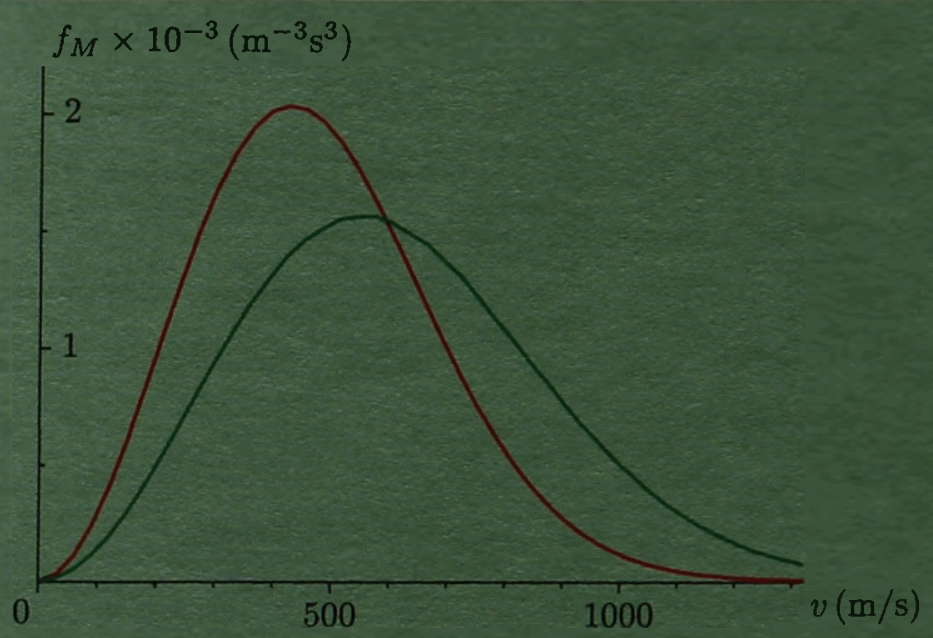
\includegraphics[width=0.4\linewidth]{mai_fig048.png}
   \captionof{figure}{Maxwellovo rozdělení rychlostí molekul dusíku pro teploty \(T_1 = 
                      \SI{300}{\kelvin}\) a \(T_2 = \SI{300}{\kelvin}\).
   \cite[s.~243]{Musilova2009MA1}
   \label{mai:fig048}}
  \par}
  
  Dokážete vyložit, proč jsme zvolili za \(\Delta\Omega\) celý objem slupky? Počítáme totiž 
  pravděpodobnost, že koncový bod vektoru rychlosti molekuly leží, zhruba řečeno, v kterémkoli 
  elementárním kvádříku \(\Delta v_x\Delta v_z\Delta v_z\) obsaženém ve slupce. A ta je součtem 
  pravděpodobností odpovídajících všem kvádříkům vytvářejícím slupku. Jedná se o pravděpodobnosti 
  navzájem neslučitelných jevů (pohybuje-li se molekula v jednom směru, nepohybuje se v jiném). 
  Hustota této pravděpodobnosti se nazývá \textbf{Maxwellovo rozdělení rychlostí}. Na rozdíl od 
  Gaussova rozdělení, popisujícího hustotu pravděpodobnosti pro jednotlivé složky rychlosti, je 
  nesymetrická vlivem faktoru \(v^2\). Obrázek \ref{mai:fig048} ukazuje funkci \(f_M(v)\) pro dvě 
  různé teploty \(T_2 > T_1\). Důležité hodnoty spjaté s tímto rozdělením jsou 
  \textbf{nejpravděpodobnější rychlost} \(v_p\), \textbf{střední rychlost} \(\langle v \rangle\) a 
  \textbf{střední kvadratická rychlost} \(\langle v^2 \rangle\). Platí
  \begin{align*}
    \der{f_M}{v}        &= 0\, \longrightarrow v_P = \sqrt{\dfrac{2kT}{m}},                      \\
    \langle v \rangle   &= \int_{-\infty}^{\infty}vf_M(v)\dd{v} = \sqrt{\dfrac{8kT}{\pi m}},     \\
    \langle v \rangle^2 &= \int_{-\infty}^{\infty}v^2f_M(v)\dd{v} = \dfrac{3kT}{m}.
  \end{align*}
\normalsize
\end{example}
      %---------------------------------------------------------------
  
  \section{Náhoda a zpracování měření}\label{mai:IchapIVsecIV}
    \subsection{Součet a součin náhodných veličin}
      Nyní vyřešíme ještě jeden důležitý problém. Víme již, že veličinu \(Y = f(X)\) lze popsat 
      stejnými pravděpodobnostmi jako veličinu \(X\). V řadě případů je však náhodná veličina \(Y\) 
      funkcí několika náhodných veličin \(X_1, X_2, \ldots, X_s\). Každá z nich má nějaké 
      rozdělení. Jaké potom bude rozdělení veličiny \(Y\)? Rozebereme jen dvě základní situace, z 
      nichž je ovšem možné „poskládat“ řadu případů složitějších. Půjde o situace, kdy náhodná 
      veličina bude součtem nebo součinem dvou náhodných veličin, pro jednoduchost značení 
      například \(U\) a \(V\), tedy \(Y = U + V\), \(Z = U \cdot V\). Předpokládejme nejprve, že 
      veličiny \(U\) a \(V\) jsou zcela nezávislé, tj. hodnoty veličiny \(U\) nejsou nijak 
      ovlivněny hodnotami veličiny \(V\) a naopak. Dejme tomu, že \(U\) a \(V\) mají rozdělení
      \begin{equation*}
        \left\lbrace (u_1, p_1), \ldots, (u_k, p_k) \right\rbrace, \qquad
        \left\lbrace (v_1, q_1), \ldots, (v_\ell, v_\ell) \right\rbrace
      \end{equation*}
      Veličiny \(Y = U + V\), resp. \(Z = U \cdot V\) tedy mohou nabývat hodnot \(\lbrace u_i + 
      v_\alpha\rbrace\), resp. \(\lbrace u_i v_\alpha\rbrace\) s pravděpodobnostmi \(p_iq_\alpha\). 
      Jevy \uv{Veličina \(U\) nabude hodnoty \(u_i\)} a \uv{veličina \(V\) nabude hodnoty 
      \(v_\alpha\)} jsou totiž nezávislé. Rozdělení veličin \(Y\) a \(Z\) je 
      \begin{equation*}
        \lbrace (u_i +v_\alpha, p_iq_\alpha)\rbrace,\, \text{resp.}\,
        \lbrace(u_iv_\alpha, p_iq_\alpha)\rbrace,\qquad 1\leq i\leq k,\quad 1\leq\alpha\leq\ell,
      \end{equation*}
      Pro jejich střední hodnoty dostáváme
      \begin{align*}
        \langle y \rangle 
          &= \sum_{i=1}^{k}\sum_{\alpha=1}^{\ell}(u_i + v_\alpha)p_iq_\alpha        \\
          &= \sum_{i=1}^{k}u_ip_i\left(\sum_{\alpha=1}^{\ell}q_\alpha\right) + 
             \sum_{\alpha=1}^{\ell}v_\alpha q_\alpha\left(\sum_{i=1}^{k}p_i\right)  \\
          &= \sum_{i=1}^{k}u_ip_i + \sum_{\alpha=1}^{\ell}v_\alpha q_\alpha         \\
        \langle z \rangle 
          &= \sum_{i=1}^{k}\sum_{\alpha=1}^{\ell}(u_i \cdot v_\alpha)p_iq_\alpha    \\
          &= \left(\sum_{i=1}^{k}u_ip_i\right)
             \left(\sum_{\alpha=1}^{\ell}v_\alpha q_\alpha\right) 
           = \langle u \rangle \langle v \rangle.
      \end{align*}
      Střední hodnota součtu, resp. součinu náhodných veličin je tedy součtem, resp. součinem jejich
      středních hodnot. Pro součet náhodných veličin platí tento výsledek i v případě, když nebudou
      nezávislé. V tak jednoduchý závěr jsme snad ani nedoufali! Hned uvidíme, jak jej lze využít.
      
      %--Jak číst výsledky studentské ankety aneb není průměr jako průměr----------
      % !TeX spellcheck = cs_CZ
\wikitextrule
\begin{example}\label{mai:exam071}
  \textbf{Jak číst výsledky studentské ankety aneb není průměr jako průměr}\newline\small
  Každý semestr na Masarykově univerzitě se uzavírá vyhodnocením velmi užitečné studentské ankety v 
  Informačním systému MU. Studenti hodnotí na jedenáctihodnotové stupnici (nula až deset bodů) 
  několik položek pro každý studijní předmět (obtížnost, zajímavost, srozumitelnost výkladu, 
  přístup učitele, rozmanitost literatury) a mohou doplnit i slovní komentáře. Na ty se učitelé 
  těší nejvíce, neboť díky anonymitě pisatelů se tak o sobě mohou dovědět leccos zajímavého. 
  Všimneme si však statistického zpracování ankety. U každého předmětu je pro danou položku 
  vypočtena průměrná bodová hodnota odpovědí a vyznačena na téže jedenáctihodnotové stupnici. Pro 
  porovnání je na stupnici vyznačen i takzvaný „fakultní průměr“. Každý přednášející může vidět svá 
  hodnocení a hodnocení svých kolegů, kteří mu vedou cvičení. Děkan má přístupové právo k celé
  statistice, a tak může porovnávat. Jednoho deštivého večera přestalo děkana bavit vyplňování 
  rektorátních formulářů a začal si výsledky ankety prohlížet. Zajímala jej zejména položka 
  „srozumitelnost výkladu“. Řekl si, že všem učitelům, kteří v této položce budou hodnoceni 
  nadprůměrně, zvýší osobní ohodnocení. Soubor předmětů je veliký, a tak děkan klikal a klikal. 
  Zjišťoval, že u veliké většiny předmětů leží průměrné hodnocení srozumitelnosti nad fakultním 
  průměrem. Jeho pocity byly smíšené. Na jedné straně se radoval, jakými jsou jeho podřízení 
  dobrými pedagogy, na druhé straně trnul, kolik to bude stát. Snad aby se raději vrátil 
  k protivným formulářům. Najednou v něm zahlodalo podezření i naděje, že není všechno v pořádku. 
  Jak je možné, že většina hodnocení leží nad průměrem? Kladné a záporné odchylky by se přece měly 
  kompenzovat. Zavolal proto na koberec proděkana pro informační technologie, aby se jej zeptal, co 
  je to „fakultní průměr“. Proděkan odpověděl takto: Máme soubor \(K\) předmětů \(\lbrace 
  X_\alpha\rbrace\), \(\alpha = 1, \ldots, K\). V předmětu \(X_\alpha\) vyplnilo anketu 
  \(N_\alpha\)  studentů, jednotlivé hodnoty odpovědí pro danou položku (srozumitelnost výkladu) 
  byly označeny \(\lbrace x_{\alpha,j}\rbrace\), \(j = 1, \ldots, N_\alpha\). Celkem přirozeně 
  předpokládáme, že váha odpovědi každého studenta je stejná, nezávisle na předmětu. Tato váha je
  rovna převrácené hodnotě celkového počtu studentů, kteří vyplnili anketu, tj. \(w = N^{-1}\), \(N 
  = N_1 + \ldots + N_k\). Fakultní průměr je proto dán vzorcem
  \begin{equation*}
    \langle x \rangle 
      = \sum_{\alpha=1}^{K}\sum_{j=1}^{N_\alpha}wx_{\alpha,j} 
      = \dfrac{1}{N}\sum_{\alpha=1}^{K}\left(\sum_{j=1}^{N_\alpha}x_{\alpha,j}\right)
      = \dfrac{1}{N}\sum_{\alpha=1}^{K}A_\alpha,
  \end{equation*}
  kde jsme označili \(A_\alpha = \sum_{j=1}^{N_\alpha}x_{\alpha,j}\). Děkan chvíli přemýšlel a 
  pravil: To vypadá docela logicky. Neměli bychom však počítat fakultní průměr tak, že vezmeme 
  průměrné hodnoty pro každý předmět a vypočteme jejich aritmetický průměr? Pak bychom dostali
  \begin{equation*}
    \langle \overline{x} \rangle
      = \dfrac{1}{K}\sum_{\alpha=1}^{K}\langle x_{\alpha}\rangle
      = \dfrac{1}{K}\sum_{\alpha=1}^{K}
        \left(\dfrac{1}{N_\alpha}\sum_{j=1}^{N_\alpha}x_{\alpha,j}\right)
      = \dfrac{1}{K}\sum_{\alpha=1}^{K}\dfrac{A_\alpha}{N_\alpha}.
  \end{equation*}
  Tento závěr se akademickým funkcionářům na první pohled nijak zvlášť nelíbil. Bylo totiž jasné, 
  že náhodné veličiny \(X_1, \ldots, X_k\) mají odlišná rozdělení. No jo, řekli si oba, musíme 
  počítat. My už ale počítat nemusíme, neboť jsme takový problém před chvílí vyřešili obecně. 
  Zjistili jsme totiž, že střední hodnota součtu náhodných veličin je rovna součtu středních 
  hodnot, bez ohledu na konkrétní rozdělení každé z veličin. Definujeme-li tedy náhodnou veličinu 
  \(Y\) jako aritmetický průměr veličin \(X_\alpha\), tj.
  \begin{align*}
    Y &= \dfrac{1}{K}\left(X_1 + \ldots + X_K\right),  \\
    \shortintertext{dostaneme}
    \langle y \rangle &= \dfrac{1}{K}\left(\langle x_1 \rangle +\ldots+\langle x_K \rangle\right).
  \end{align*}
  Tento výsledek se shoduje s hodnotou \(\langle \overline{x} \rangle\), kterou pro výpočet 
  „fakultního průměru“ navrhl děkan. Vypočteme-li součet odchylek hodnot \(\langle x_\beta 
  \rangle\) od \(\langle y \rangle\), dostaneme skutečně nulu:
  \begin{equation*}
    \sum_{\beta =1}^{K}\left(\langle x_\beta \rangle - \langle y \rangle\right)
      = \sum_{\beta =1}^{K}\left(\dfrac{A_\beta}{N_\beta} 
      - \dfrac{1}{K}\sum_{\alpha=1}^{K}\langle x_\alpha \rangle\right)
      = 0.
  \end{equation*}
  Zkusme se ještě zamyslet nad tím , jak použití „špatného“ fakultního průměru zkreslilo výsledky a 
  proč. Vypočtěme si rozdíl \(\Delta = \langle \overline{x} \rangle - \langle x \rangle\):
  \begin{equation*}
    \Delta = \langle \overline{x} \rangle - \langle x \rangle 
      = \dfrac{1}{K}\sum_{\alpha=1}^{K}\langle x_\alpha \rangle
      - \dfrac{1}{N}\sum_{\alpha=1}^{K}A_\alpha
      = \dfrac{1}{K}\sum_{\alpha=1}^{K}\langle x_\alpha \rangle
      - \dfrac{1}{N}\sum_{\alpha=1}^{K}N_\alpha\langle x_\alpha \rangle
      = \dfrac{1}{K}\sum_{\alpha=1}^{K}\langle x_\alpha\rangle\left(1 - K\dfrac{N_\alpha}{N}\right).
  \end{equation*}
  Platí přitom
  \begin{equation*}
    \sum_{\alpha=1}^{K}\left(1 - K\dfrac{N_\alpha}{N}\right) = 0.
  \end{equation*}
  Pokud by byl počet studentů, kteří vyplnili anketu, ve všech předmětech stejný, tj. \(N_\alpha = 
  \dfrac{N}{K}\) , byla by odchylka \(\Delta\) podle očekávání nulová. Stejná situace by nastala, 
  kdyby byly shodné všechny průměrné hodnoty \(\langle x_\alpha \rangle\). Je-li odchylka 
  \(\Delta\) kladná, je „nesprávný“ fakultní průměr \(\langle x \rangle\) nižší než \(\langle 
  \overline{x} \rangle\). Proto hodnocení jednotlivých předmětů vypadají příznivěji, právě tak, jak 
  to zjistil děkan. Odchylku \(\Delta\) posouvají do kladných hodnot předměty, které hodnotilo málo 
  studentů, a předměty, které měly vysoké hodnocení. Dobře je to vidět na příkladu dvou předmětů, 
  tj. pro \(K = 2\), kde vychází
  \begin{equation*}
    \Delta = \langle \overline{x} \rangle - \langle x \rangle 
           = \dfrac{N_2 - N_1}{2(N_2+N_1)}\left(\langle\overline{x}\rangle-\langle x\rangle\right).
  \end{equation*}
  
  Pro \(N_1\ll N_2\) a \(\langle x_1 \rangle  \gg \langle x_2 \rangle \) bude rozdíl \(\Delta\) 
  skoro polovina hodnoty \(\langle x_1 \rangle\)! U volitelných specializovaných předmětů, které si 
  vybírají jen poměrně malé počty studentů, kteří navíc mají o předmět opravdový zájem a hodnotí 
  jej proto většinou vyšším počtem bodů, je splněno obojí (malý počet hodnotících a vysoké bodové
  hodnocení). Je vidět, že při nesprávně zvoleném výpočtu srovnávací hodnoty (fakultního průměru) 
  mohou právě předměty, jejichž statistický význam je spíše okrajový, ovlivnit celkové hodnocení.
\normalsize
\end{example}
      %----------------------------------------------------------------------------
      
      Pro střední hodnotu součtu a součinu nezávislých náhodných veličin jsme získali velmi
      jednoduché výsledky:
      
      \begin{mdframed}[style=highlight]
        \begin{equation}\label{mai:eq070}
          \langle u + v \rangle = \langle u \rangle + \langle v \rangle\quad
          \langle uv \rangle    = \langle u \rangle \langle v \rangle.
        \end{equation}
      \end{mdframed}
      
      Dokážeme také určit rozptyl veličin \(Y = U + V\) a \(Z = U\cdot V\)? Pro rozptyl každé 
      náhodné veličiny platí obecný vztah (\ref{mai:eq061}). Použijeme jej pro naše konkrétní 
      případy:
      \begin{gather*}
        \begin{align*}
          D(U + V) &= \langle (u + v)^2 \rangle - \langle u + v \rangle^2                     \\
                   &= \langle u^2 + 2uv + v^2 \rangle - \left(\langle u \rangle^2 +
                      \langle 2uv \rangle + \langle v^2 \rangle\right)                        \\
                   &= \left(\langle u^2\rangle - \langle u \rangle^2\right)
                    + \left(\langle v^2\rangle - \langle v \rangle^2\right) = D(U) + D(V).
        \end{align*}
      \end{gather*}
      Pro rozptyl náhodné veličiny \(Z = U \cdot V\) dostaneme
      \begin{align*}
        D(Z)  &= \langle z^2\rangle - \langle z \rangle^2 
               = \langle u^2\rangle\langle v^2\rangle - \langle u \rangle^2 \langle v \rangle^2  \\
              &= \left[D(U) + \langle u^2\rangle\right]\left[D(V) + \langle v^2\rangle\right]
               - \langle u \rangle^2 \langle v \rangle^2                                         \\
              &= D(U)D(V) + \langle u \rangle^2D(V) + \langle v \rangle^2D(U).
      \end{align*}
      Pak
      \begin{mdframed}[style=highlight]
        \begin{equation*}
          \dfrac{D(z)}{ \langle z \rangle^2} = \dfrac{D(U)}{ \langle u \rangle^2} \cdot
            \dfrac{D(V)}{ \langle v \rangle^2} + \dfrac{D(U)}{ \langle u \rangle^2} +
            \dfrac{D(v)}{ \langle v \rangle^2}.
        \end{equation*}
      \end{mdframed}
      Při výpočtu jsme využili vztahu (\ref{mai:eq061}) a vztahů (\ref{mai:eq070}) pro střední 
      hodnotu součtu a součinu náhodných veličin. Pokud mají veličiny \(U\) a \(V\) shodný rozptyl 
      \(D(U) = D(V) = D\), pak je \(D(U + V) = 2D\). V případě součtu s veličin \(Y = X_1 + \cdots 
      + X_s\) se shodným rozptylem \(D\) resp. směrodatnou odchylkou \(\sigma\) dostáváme
      \begin{equation*}
        D(Y) = sD  \Rightarrow \sigma(y) = \sqrt{s}\sigma.
      \end{equation*}
      Znovu připomeňme, že všechny vztahy týkající se součtu a součinu náhodných veličin, které
      jsme zatím získali, platí za předpokladu, že výchozí veličiny, které sčítáme nebo násobíme, 
      jsou nezávislé.
      
      Aniž bychom se podrobněji zabývali vlastnostmi rozdělení závislých veličin, definujeme pro
      ně charakteristiky, které tuto závislost popisují. Nechť \(U\) a \(V\) jsou dvě libovolně 
      náhodné veličiny, ne nutně nezávislé. Míru jejich závislosti určují veličiny
      \begin{subequations}\label{mai:eq071}
        \begin{align}
          \sigma_{uv} 
            &= \langle (u - \langle u \rangle) (v - \langle v \rangle) \rangle,  \\
          \varrho_ {uv}
            &=\dfrac{\sigma(u)}{\sqrt{D(U)D(V)}} = \dfrac{\sigma(u)}{\sigma{D(u)\sigma(v)}}
        \end{align}
      \end{subequations}  
      zvané \textbf{kovariance} a \textbf{korelační koeficient} veličin \(U\) a \(V\). Platí 
      \(\varrho(uv) \leq 1\). Pro nezávislé veličiny vychází \(\sigma(uv) = 0\) a \(\varrho(uv) = 
      0\).
      
      %-- Rozptyl při Bernoulliově pokusu-----------------------------
      % !TeX spellcheck = cs_CZ
\begin{mdframed}[style=mdexam]
  \begin{example}\label{mai:exam072}
    \textbf{Rozptyl při Bernoulliově pokusu}\newline
    V příkladu \ref{mai:exam066} jsme se zajímali o střední hodnotu veličiny \(X\) definované jako
    počet zdarů při \(n\) opakováních Bernoulliova pokusu. Řekli jsme si, že střední hodnota této
    veličiny je \(np\) s tím, že důkaz lze provést přímo na základě definičního vztahu pro střední
    hodnotu matematickou indukcí. Výpočet rozptylu z definičního vztahu bychom jistě snadno dokázali
    zahájit, horší by však bylo dovést jej do konce. Stačí se podívat na začátek výpočtu
    \begin{align*}
      D(X) &= \sum_{j=0}^n \left(x_j - \langle x \rangle\right)^2p_j             \\
           &= \sum_{j=0}^n \left(j - np\right)^2\binom{n}{j}p^j(1 - p)^j,
    \end{align*}
    a nepochybujeme o tom, že tuto sumu nedokážeme spočítat snadno. Protože již však umíme zacházet
    se součtem náhodných veličin, můžeme využít účinného triku. Veličinu \(X\) si představíme jako
    součet
    \begin{equation*}
      X = U_1 + U_2 + \cdots + U_n,
    \end{equation*}
    kde každá z veličin \(U_j\) může nabývat dvou hodnot. Jedničky v případě, že při \(j\)-tém
    opakování pokusu nastal zdar, a nuly v případě, že nastal nezdar. Součet všech veličin \(U_j\)
    pro \(j = 1\) až \(j = n\) pak skutečně znamená celkový počet zdarů při \(n\) opakováních
    pokusu. Jestliže si uvědomíme, že pravděpodobnost zdaru při kterémkoli z opakování je \(p\) a
    pravděpodobnost nezdaru \((1 - p)\), ihned vidíme, že rozdělení každé z veličin \(U_j\) má tvar
    \(\lbrace(1, p), (0, 1 - p)\rbrace\). Platí tedy
    \begin{equation*}
      \langle u_j\rangle = 1\cdot p + 0 \cdot (1 - p) = p,
    \end{equation*}
    \begin{align*}
      D = D(U_j) &= \left( 1 - \langle u_j\rangle\right)^2p 
                  + \left( 0 - \langle u_j\rangle\right)^2(1 - p)   \\
                 &= p(1 - p)^2 + p^2(1 - p) = p(1 - p).
    \end{align*}
    Každé dvě veličiny \(U_i\), \(U_j\) jsou nezávislé, neboť jednotlivá opakování pokusu jsou
    nezávislá. Střední hodnota jejich součtu je: tedy \(np\) (a to souhlasí s informací v příkladu
    \ref{mai:exam066}) a pro rozptyl jejich součtu platí
    \begin{equation*}
      D(X) = nD = np(1 - p).
    \end{equation*}
    Celkově tedy dostáváme
    \begin{equation*}
      \langle x \rangle = np, \; \sigma(x) = \sqrt{np(1 - p)}.
    \end{equation*}
  \end{example}
\end{mdframed}
      %---------------------------------------------------------------
      
      %-- Rozptyl aritmetického průměru-------------------------------
      % !TeX spellcheck = cs_CZ
\begin{mdframed}[style=mdexam]
  \begin{example}\label{mai:exam073}
    \textbf{Rozptyl aritmetického průměru}\newline
    Již v úvodu odstavce o náhodných veličinách jsme konstatovali, že opakujeme-li v nezměněných
    podmínkách měření jisté fyzikální veličiny (délka závěsu kyvadla, proud procházející vodičem,
    napětí na vodiči, atd.), budeme díky náhodným vlivům dostávat pokaždé poněkud jiný výsledek.
    Říkáme, že měření je zatíženo náhodnými chybami. Výsledek získaný při každém opakování lze
    interpretovat jako hodnotu náhodné veličiny. Dejme tomu, že jsme provedli uměření fyzikální
    veličiny \(X\) a získali hodnoty \(x_1\) až \(x_n\) . V praktické situaci budou tyto hodnoty
    většinou navzájem různé, nemusí tomu tak však nutně být. Fyzikální veličinu chceme ovšem
    reprezentovat jediným údajem, a tím bude její střední hodnota, tj.
    \textbf{aritmetický průměr}
    \begin{equation*}
      \langle x \rangle = \dfrac{x_1 + x_2 + \cdots + x_n}{n}.
    \end{equation*}
    Rozptyl veličiny \(X\) je dán vztahem
    \begin{align*}
      D &= D(X)                                                             \\
        &= \dfrac{\left(x_1 - \langle x \rangle\right)^2 + 
                  \left(x_2 - \langle x \rangle\right)^2 + \cdots +
                  \left(x_n - \langle x \rangle\right)^2}{n}.
    \end{align*}
    Víme, že směrodatná odchylka \(\sigma( x ) = \sqrt{D(X)}\) určuje, nakolik jsou jednotlivé
    výsledky měření v průměru odchýleny od střední hodnoty, charakterizuje tedy přesnost každého
    opakování měření. Podívejme se na celou úlohu z jiné strany: Představme si, že sledujeme \(n\)
    po dvou nezávislých náhodných veličin \(X_1\) až \(X_n\) se shodnou střední hodnotou \(\langle
    x_j \rangle = \langle x \rangle\) a shodnou směrodatnou odchylkou \(\sigma(x_j) = \sqrt{D},\, 1
    \leq j \leq n\). Aritmetický průměr těchto veličin,
    \begin{equation*}
      \langle \Xi \rangle = \dfrac{X_1 + X_2 + \cdots + X_n}{n}.
    \end{equation*}
    je tedy rovněž náhodnou veličinou. Pro jeho střední hodnotu, rozptyl a směrodatnou odchylku
    platí
    \begin{align*}
      \langle \xi \rangle 
                  &= \dfrac{n\langle x \rangle}{n}, \\
      D(\Xi)      &= \dfrac{1}{n^2}\cdot D(X_1 + \cdots + X_n)=\dfrac{nD^2}{n^2}=\dfrac{D}{n}, \\
      \sigma(\xi) &= \dfrac{\sigma(x)}{\sqrt{n}}.
    \end{align*}
  \end{example}
\end{mdframed}
      %---------------------------------------------------------------
      
      Můžeme tedy říci, že aritmetický průměr všech výsledků měření dané fyzikální veličiny je
      \(\sqrt{n}\)-krát přesnější než jednotlivý výsledek měření. Jakkoli se toto konstatování zdá 
      intuitivně zřejmé, je třeba je používat s opatrností.
      
      Především je třeba mít na mysli, co toto konstatování znamená. Jeho charakter je totiž
      opět jen pravděpodobnostní. Jestliže jsou jednotlivá měření prováděna za stejných podmínek,
      jsou rozdělení veličin \(X_1\) až \(X_n\) funkcemi téhož typu. Tyto veličiny mají také 
      stejnou střední hodnotu \(\langle x \rangle\) a směrodatnou odchylku \(\sigma\). Také 
      pravděpodobnost, že při měření padne hodnota veličiny \(X_j\) do intervalu \((\langle x 
      \rangle - \sigma, \langle x \rangle + \sigma)\), je pro všechna \(j\) prakticky stejná. 
      Označme ji \(P_\sigma\).  Se stejnou pravděpodobností nabude aritmetický průměr \(\Xi\) 
      hodnoty v intervalu určeném svou směrodatnou odchylkou. Ta je však \(\sqrt{n}\)-krát menší. V 
      tomto smyslu jsou hodnoty aritmetického průměru \uv{\(\sqrt{n}\)-krát méně rozptýleny} kolem 
      střední hodnoty \(\langle\xi \rangle\) než hodnoty náhodných veličin \(X_j\) kolem svých 
      středních hodnot \(\langle x \rangle\).
      
      Dalším problémem může být splnění výchozích předpokladů, které vedly ke vztahu pro
      směrodatnou odchylku aritmetického průměru. Ukážeme to na následujícím příkladu.
      
      %-- Jak přesně lze změřit čínského císaře?----------------------
      % !TeX spellcheck = cs_CZ
\wikitextrule
\begin{example}\label{mai:exam075}
  \textbf{Ověření Ohmová zákona}\newline\small

\normalsize
\end{example}
      %---------------------------------------------------------------
      
      %-- Záhada přijímací zkoušky aneb k čemu může posloužit distribuční funkce-----
      % !TeX spellcheck = cs_CZ
\begin{mdframed}[style=mdexam]
  \begin{example}\label{mai:exam075}
    \textbf{Záhada přijímací zkoušky aneb k čemu může posloužit distribuční funkce?}\newline
    Mohlo by se zdát, že distribuční funkce je jen teoretický pojem a že v praktických situacích ji
    těžko využijeme. Podstatné je přece pravděpodobnostní rozdělení náhodné veličiny a distribuční
    funkce je z něj jen jaksi odvozena sčítáním pravděpodobností (u diskrétního rozdělení) nebo
    integrací (u rozdělení spojitého). Přesvědčíme se, že existují velmi realistické případy, kdy
    distribuční funkce přináší věrohodnější informaci o náhodné veličině než samotné rozdělení.
    
    Na Masarykově univerzitě musí každý uchazeč o studium, ať již se hlásí na přírodovědeckou,
    právnickou, lékařskou či jinou fakultu, absolvovat Test studijních předpokladů. Jedná se o
    všeobecný test, zaměřený na zjišťování úrovně všech schopností uchazeče, které jsou potřebné pro
    univerzitní studium, například analytického myšlení, verbálních schopností, numerického myšlení,
    geometrické představivosti, atd. Pro nás však v tu to chvíli není podstatný obsah testu, ale
    způsob zpracování jeho výsledků a vyhodnocení pořadí uchazečů. Test skládá kolem třiceti tisíc
    studentů. Není tedy možné technicky zajistit, aby proběhl v jediné variantě v jednom dni. K
    dispozici je proto osm variant testu, každou variantu řeší tři až čtyři tisíce studentů. Test má
    \num{80} otázek, základním údajem pro zpracování jeho výsledků je počet správných odpovědí
    každého studenta. Pokud bychom označili jako \(i\) počet správných odpovědí (\(i \in\lbrace0, 1,
    2, \ldots, 80\rbrace\)) v kterékoli variantě a \(\mathcal{N}_i\) počet studentů, kteří dosáhli
    právě \(i\) správných odpovědí, dostaneme náhodnou veličinu \(X_i\), kterou bychom mohli nazvat
    „počet správných odpovědí“, pro celou univerzitu. Její rozdělení by mělo tvar
    \begin{equation*}
      \lbrace(i,p_i)\rbrace,\quad\text{kde}\qquad p_i = \dfrac{\mathcal{N}_i}{\mathcal{N}}, \quad
      \mathcal{N} = \sum_{i=0}^{80}\mathcal{N}_i
    \end{equation*}
    A zde je malý „kámen úrazu“. A by bylo možné sestavit opravdu „univerzální pořadí“, musely by
    být všechny varianty testu ekvivalentní z hlediska obtížnosti. To znamená, že kdyby kterýkoli
    student vyplnil za stejných podmínek všechny varianty, dosáhl by v každé z nich stejného počtu
    správných odpovědí s pravděpodobností velmi blízkou jedné. Skutečnost je však principiálně
    taková, že u sebelépe promyšleného a sestaveného testu se jednotlivé varianty budou mírně, v
    rámci statistických, a tedy již neodstranitelných, odchylek lišit. Tato odlišnost se nepozná
    předem, ale až po zpracování výsledků všech variant. Použít pro stanovení pořadí uchazečů
    rozdělení náhodné veličiny \(X\) \emph{= počet správných odpovědí je tedy nespravedlivé}.
    Student, který řešil variantu „statisticky obtížnější“, by v pořadí skončil s horším umístěním,
    než student, který je stejně schopný, avšak měl to štěstí, že na něj připadla varianta
    „statisticky méně obtížná“. Skutečně, kdybychom sestavili grafy rozdělení náhodných veličin
    \(X^{(\alpha)}\) \emph{= počet správných odpovědí v \(\alpha\)-té variantě},
    \begin{equation*}
      \lbrace(i,p_i^{(\alpha)})\rbrace,\quad\text{kde}\; 
      p_i^{(\alpha)} = \dfrac{\mathcal{N}_i^{(\alpha)}}{\mathcal{N}^{(\alpha)}}, \quad
      \mathcal{N}^{(\alpha)} = \sum_{i=0}^{80}\mathcal{N}_i^{(\alpha)}
    \end{equation*}
    zjistili bychom, že se mírně liší. (V předchozím zápisu značí \(\mathcal{N}_i^{(\alpha)}\) počet
    studentů, kteří odpověděli správně na \(i\) otázek \(\alpha\)-té varianty
    \(\mathcal{N}^{(\alpha)}\) je počet všech studentů, kteří tuto variantu řešili.) Střední hodnoty
    i mediány náhodných veličin se i při vynikající shodě obtížnosti všech variant mohou lišit v
    rozmezí jedné až dvou správných odpovědí. A s ohledem na skutečnost, že každou variantu řeší
    obrovský počet studentů, až čtyři tisíce, je zřejmé, že tento rozdíl může poněkud „zamíchat
    “pořadím, zejména v blízkosti mediánu, kde se týká třeba i tří stovek studentů v každé variantě.
    Situaci dokládá obrázek \ref{mai:fig049}. Jak tedy zařídit, abychom dostali spravedlivé pořadí?
    Jediný rozumný způsob, jak minimalizovat vliv statistických odchylek obtížnosti jednotlivých
    variant, je nehodnotit studenty podle absolutního počtu správných odpovědí, ale nějak je
    porovnat mezi sebou. Budeme při tom předpokládat, že rozložení schopností studentů je ve všech
    osmi skupinách, které řeší osm daných variant, stejné. Řeknete si - zase nějaké další
    předpoklady. To je jako z bláta do louže. Předpoklad o stejném rozložení schopností studentů v
    tak velkých skupinách, jako jsou ty naše, je však mnohem realističtější než předpoklad o
    dokonalé shodě obtížnosti variant testu. Budeme se jej proto držet. Každému studentovi
    přisoudíme číslo, které informuje o tom, kolik řešitelů dané varianty bylo horších nebo stejně
    dobrých jako on, tj. mělo nižší nebo stejný počet správných odpovědí. Z matematického hlediska
    to znamená přejít v každé variantě od rozdělení k distribuční funkci. Věnujme se nyní tomuto
    přepočtu podrobněji jak pro diskrétní rozdělení náhodné veličiny \(X^{(\alpha)}\), které
    odpovídá skutečné situaci, tak pro zajímavost i pro rozdělení spojité. V dalším budeme vždy
    zpracovávat výsledky jedné varianty, upustíme proto od vyznačování indexu \(\alpha\).

    {\centering
    \captionsetup{type=figure}
    \luafigure[0.8]{mai_fig049.png}
    \captionof{figure}{Rozdělení pro dvě varianty testu,
    \cite[s.~252]{Musilova2009MA1}
    \label{mai:fig049}}
    \par}
    
    \textbf{Diskrétní rozdělení}
      \begin{itemize}
        \item \emph{Zadání:} Skupina \(N\) studentů řeší jednu variantu testu. Test má \(Q\) otázek.
              Za každou správnou odpověď je přidělen jeden výchozí bod. Získáváme rozdělení
              \begin{gather*}
                \left\lbrace\left(i, \dfrac{N_i}{N} \right)\right\rbrace, \;
                i\in\lbrace0, 1, 2, \ldots, Q\rbrace, \;
                \sum_{i=0}^{Q}N_i = N 
              \end{gather*}
              kde \(i\) je počet výchozích bodů a \(N_i\) počet studentů, kteří získali \(i\) bodů.
              Distribuční funkce tohoto rozdělení
              \begin{gather*}
                F(x) = \dfrac{1}{N}\sum_{i=0}^{j}N_i\;\text{ pro }\;
                j\leq x < j+1, \; x\in\left[0,\infty\right)
              \end{gather*}
              Pro uchazeče, který získal \(j\) bodů, mají význam následující hodnoty:
              \begin{itemize}
                \item \(F(x)    x \in \left[j, j+1\right)\): poměrný počet uchazečů, kteří získali
                      počet výchozích bodů nižší nebo shodný s daným uchazečem,
                \item \(NF(x)   x \in \left[j, j+1\right)\): absolutní počet uchazečů, kteří získali
                      počet výchozích bodů nižší nebo shodný s daným uchazečem,
                \item \(100F(x) x \in \left[j, j+1\right)\): absolutní počet uchazečů, kteří získali
                      počet výchozích bodů nižší nebo shodný s daným uchazečem,
              \end{itemize}
        \item Hodnoty distribuční funkce můžeme získat z následující tabulky:
        
              {\centering
                \resizebox{0.8\textwidth}{!}{%
                \begin{tabular}{c|c}
                          interval \(x\)     &  \(NF(x)\)         \\ \hline
                  \(\left[0,1\right)\)       &  \(N_0\)           \\ 
                  \(\left[1,2\right)\)       &  \(N_0 + N_1\)     \\ 
                  \(\cdots\)                 &  \(\cdots\)        \\
                  \(\left[j,j+1\right)\)     &  \(N_0 + N_1 + \cdots + N_j\) \\ 
                  \(\cdots\)                 &  \(\cdots\) \\
                  \(\left[Q-1,Q\right)\)     &  \(N_0 + N_1 + \cdots + N_{Q-1}\) \\ 
                  \(\left[Q,\infty\right)\)  &  \(N_0 + N_1 + \cdots + N_{Q} = N\) 
                \end{tabular}}
              \par}
        \item Přepočet hodnocení uchazečů tak, aby nová stupnice byla opět v rozsahu mezi nulou a
              \(Q\) a aby nové hodnocení bylo opět celočíselné, je následující:
              \begin{equation*}
                y =QF(x), \quad 0\leq F(x) \leq 1, \Rightarrow y \in[0,Q].
              \end{equation*}
              Uchazeči se ziskem \(i\) výchozích bodů náleží hodnota \(y = QF(x)\) právě když i\(
              \in \left[i, i + 1\right)\), tj. \(y_i = Q F(i)\). Tato hodnota není obecně
              celočíselná. Zaokrouhlení se provede ve prospěch uchazeče, tedy vždy nahoru. Výsledný
              převodní vzorec je
              \begin{equation*}
                \begin{multlined}
                  \text{výchozí body } i \longrightarrow\text{ nové body }  \\ 
                  \shoveleft[1cm]Y_i: Y_i = [y_i] + 1 = [QF(i)] + 1,
                \end{multlined}
              \end{equation*} 
              kde \([a]\) značí celočíselnou část čísla \(a\), tedy například \([\num{23.05}] =
              [\num{23.48}] = [23,89] = 23\)
        \item Zaveďme novou náhodnou veličinu \(Z\) s rozdělením \(\left\lbrace(z_\alpha,
              M_\alpha)\right\rbrace\): Označme \(z_1, z_2, \ldots, z_\alpha, ...,\) \(z_S\)
              navzájem různé hodnoty ze souboru \(\lbrace Y_i\rbrace, i = 0, 1, 2, \ldots, Q\)
              řazené vzestupně. Její rozdělení udává kterákoli z následujících tabulek:

              {\centering
                \resizebox{0.9\textwidth}{!}{%
                \begin{tabular}{c|c}
                          hodnota                       &  četnost         \\
                          \hline
                  \(z_1 = Y_0 = Y_1 = \cdots Y_{i_1}\)  & \(M_1 = N_0 + N_1 + \cdots + N_{i_1}\)  \\ 
                  \(Z_2 = Y_{i_1+1} = \cdots Y_{i_2}\)  & \(M_2 = N_{i_1+1} + \cdots + N_{i_2}\)  \\ 
                  \(\cdots\)                            & \(\cdots\)                              \\
                  \(Z_S = Y_{i_{S-1}+1}=\cdots Y_{i_S}\)& \(M_S = N_{i_{S_1}+1}+\cdots+N_{i_S}\)   
                \end{tabular}}
              \par}

              {\centering
                \resizebox{0.9\textwidth}{!}{%
                \begin{tabular}{c|c}
                          hodnota                        &  četnost         \\
                          \hline
                  \(z_1 = Y_0 = Y_1 = \cdots Y_{i_1}\)   &  \(M_1 = NF(i_1)\)              \\
                  
                  \(Z_2 = Y_{i_1+1} = \cdots Y_{i_2}\)   &  \(M_2 = N[F(i_2) - F(i_1)]\)  \\ 
                  \(\cdots\)                             &  \(\cdots\)                     \\
                  \(Z_S = Y_{i_{S-1}+1}=\cdots Y_{i_S}\) & \(M_S = N[F(i_S) - F(i_{S-1})]\)   
                \end{tabular}}
              \par}
              kde \(i_1 < i_2 < \ldots < i_{S-1} < i_S, i_S = Q\) (Vzhledem k zaokrouhlování nahoru
              není žádná bodová hodnota \(Y_i\) nulová.) I když skutečné rozdělení při zpracování
              výsledků testů je diskrétní, ukažme si, jak by vypadal analogický postup u rozdělení
              spojitého, kde je početní zpracování názornější.
      \end{itemize}
    
    \textbf{Spojité rozdělení}
      \begin{itemize}
        \item \emph{Zadání:} Je dáno rozdělení četností \(n(x) \leq 0,\, x \in [0, Q]\).
        \item Normovací podmínka a distribuční funkce jsou
              \begin{equation*}
                \int_{0}^{Q}n(x)\dd{x} = N, \quad 
                F(x) = \dfrac{1}{n}\int_{0}^{x}n(\xi)\dd{\xi},                
              \end{equation*}
              kde \(0 \leq F(x) \leq 1.\)
        \item Označme \(z = QF(x)\), tedy \(z \in [0, Q]\), novou náhodnou veličinu. (Uvědomme si,
              že \(z\) je rostoucí funkcí proměnné \(x\)). Označme její rozdělení \(\nu(z)\). Její
              distribuční funkce je
              \begin{align*}
                \Phi(z) &= \int_{0}^{z}\nu(\zeta)\dd{\zeta} 
                         = \int_{0}^{x(z)}\dfrac{n(\xi)}{N}\dd{\xi}          \\
                        &= F\left(F^{-1}(z/Q)\right) 
                        = \dfrac{z}{Q}, \quad
                \nu(z) = \dfrac{1}{Q}.
              \end{align*}
        \item Rozdělení je konstantní s mediánem i střední hodnotou \(Q/2\). Takové rozdělení se
              nazývá rovnoměrné.
      \end{itemize}
  \end{example}
\end{mdframed}
      %------------------------------------------------------------------------------
      
    \subsection{Který výsledek je ten pravý?}
      První věc, kterou budete dělat ve fyzikálním praktiku, bude zjišťování průměrné hustoty 
      materiálu, z něhož je vyroben kovový váleček. Budete váleček vážit, abyste určili jeho 
      hmotnost,a měřit jeho výšku a průměr, abyste mohli vypočítat jeho objem. Hustotu stanovíte 
      jako podíl hmotnosti a objemu. Jedná se stále o jeden a týž váleček, jehož průměrná hustota 
      má za daných podmínek (stálá teplota, váleček se nedeformuje, apod.) stále stejnou „správnou“ 
      hodnotu, kterou však neznáme. (Nezná ji ani učitel v praktiku, i když se tak tváří.) Změří-li 
      hustotu válečku všichni studenti ve skupině, každý jen jednou, získá se řada různých hodnot. 
      Která z nich je ta správná? Není vyloučeno, a je to dokonce velmi pravděpodobné, že žádná. A 
      mohli bychom pomocí nich správnou hodnotu určit nebo se k ní alespoň přiblížit? Možné by to 
      bylo, pokud bychom zaručili, že všechny výsledky získané jednotlivými studenty jsou „stejně 
      hodnotné“. Znamenalo by to, že bychom museli vyloučit hrubé a systematické chyby, které by 
      vznikly třeba tak, že by někteří studenti vážili na vadných vahách, někteří by měli špatné 
      měřítko, popřípadě by odečítali údaj „zboku“, takže by byl zkreslený, nebo by se dokonce 
      zmýlili při odečítání údaje. Museli bychom také zaručit, že náhodné vlivy, které ovlivňují 
      měření, zatěžují je náhodnými chybami a v principu je nelze odstranit, byly při všech 
      měřeních stejné. U různých studentů si tím však nemůžeme být jisti (vzpomeňte si na měření 
      čínského císaře), proto budeme raději postupovat tak, že jeden pečlivý student provede větší 
      počet měření třeba výšky válečku, která je pro určení hustoty potřebná. Dejme tomu, že bude 
      měřit milimetrovým měřítkem a bude odhadovat s přesností na půl milimetru. Jeho údaje tedy 
      mohou mít tvar \SI{33.0}{\mm}, \SI{34.5}{\mm}, atd. Získá takto za stejných podmínek třeba 
      dvacet nebo i padesát hodnot, ale co teď s nimi? Jak určit hodnotu, která se bude nejvíce 
      blížit správné hodnotě výšky válečku? (Dalo by se jistě diskutovat i o tom, co je to správná 
      hodnota. Pro tuto chvíli však předpokládejme, že taková hodnota skutečně existuje, neboť 
      váleček je opravdu válcem, je vysoustružen pečlivě, přesněji, než jsme schopni jej měřit, při 
      měření se nemění teplota, váleček není dáván do lisu a deformován, ani upravován tak, že by 
      se měnila jeho hmotnost.) Předpokládejme, že správná hodnota výšky válečku je \(x\) a že 
      student naměřil hodnoty \(\lbrace x_1, X_2, \ldots, x_n\rbrace\), mezi nimiž mohou být 
      pochopitelně i některé hodnoty stejné. Odchylky jeho měření od správné hodnoty jsou
      \begin{equation*}
        \lbrace \varepsilon_1, \varepsilon_2, \ldots, \varepsilon_n\rbrace, \qquad
        \varepsilon_i = x_i - x, \qquad i = 1, 2, \ldots, n.
      \end{equation*}
      I kdybychom správnou hodnotu \(x\) znali, nedokázali bychom předpovědět, nakolik se od ní při
      jednotlivém měření odchýlíme. Můžeme, se však zajímat o to, jaká je pravděpodobnost, že
      hodnota, o kterou bude měření od správné hodnoty odkloněno, bude ležet v určitém intervalu.
      Odchylky \(\varepsilon_i\) lze totiž interpretovat jako hodnoty náhodné veličiny. Abychom 
      mohli požadované pravděpodobnosti určit, potřebujeme znát rozdělení této veličiny. Označme ji 
      \(\varepsilon\) a odpovídající hustotu pravděpodobnosti \(\mathcal{w}(\varepsilon)\). Toto 
      rozdělení je za určitých podmínek \textbf{rozdělením normálním}, splňuje tedy vztah 
      (\ref{mai:eq069}). Zkusme se o tom přesvědčit. Zvolme podmínky měření tak, aby byly ve hře 
      jen náhodné chyby způsobené \(m\) nezávislými vlivy. Každý z nich hodnotu měření
      odchýlí od \(x\) o stejně velkou hodnotu \(\alpha\), kladnou nebo zápornou, s 
      pravděpodobností \num{0.5}. Schéma této úvahy je na obrázku \ref{mai:fig050}. Výsledná 
      odchylka naměřené hodnoty \(x_i\) od hodnoty správné s jistotou leží v intervalu \((-m\alpha, 
      m\alpha)\) a může nabývat pouze hodnot celých násobků \(\alpha\). Při uplatnění jednotlivého 
      „chybového“ vlivu vzniká, jak jsme již řekli, kladná nebo záporná odchylka o velikosti 
      \(\alpha\). Vznik odchylky \(+\alpha\) nazveme zdarem, vznik odchylky \(-\alpha\) nezdarem.
      
      \luagraphic[1]{mai_fig050.png}{Vznik kladných a záporných odchylek při měření s \(m\) vlivy. 
      \cite[s.~255]{Musilova2009MA1}}{mai:fig050}
     
      Mohlo by tomu být i naopak, slova „zdar“ a „nezdar“ zde nemají svůj obvyklý význam, jde
      pouze o to, že díky nim můžeme hned uvidět souvislost s Bernoulliovým pokusem a tedy
      i s Bernoulliovým rozdělením. Při \(j\) kladných a \(m - j\) záporných odchylkách je měření od
      správné hodnoty odkloněno o
      \begin{equation*}
        j\alpha + (m - j)(-\alpha) = (2j - m)\alpha
      \end{equation*}
      s pravděpodobností
      \begin{equation*}
        p_j = \binom{m}{j}p^j(1 - p)^{m - j} = 2^{-m}.
      \end{equation*}
      Střední hodnota náhodné veličiny \(\varepsilon\) je nulová. Skutečně, v příkladu 
      \ref{mai:exam066} jsme zjistili, že střední hodnota veličiny \(Y\) nabývající hodnot \(y_j = 
      j\) s Bernoulliovým rozdělením je \(\langle y \rangle = mp\), střední hodnota veličiny \((2j 
      - m)\) a pak musí být \((2mp - m)\alpha\). Pro \(p = \num{0.5}\) je tato hodnota nulová.
      Pro velká \(m\) lze Bernoulliovo rozdělení nahradit rozdělením normálním (obr. 3.8), a proto 
      má náhodná veličina \(\varepsilon\) hustotu pravděpodobnosti tvaru (\ref{mai:eq069}), tj.
      \begin{equation*}
        \mathcal{w}(\varepsilon) = 
        \dfrac{1}{\sigma\sqrt{2\pi}}\exp\left(\dfrac{-\varepsilon^2}{2\sigma^2}\right).   
      \end{equation*}

      \luagraphic[0.8]{mai_fig051.png}{Normální rozdělení jako limitní případ Bernoulliova 
      \cite[s.~256]{Musilova2009MA1}}{mai:fig051}
    
      Vraťme se nyní k otázce zpracování naměřených hodnot \(\lbrace x_1, \ldots, x_n\rbrace\) 
      výšky válečku. Jejich odchylky od správné hodnoty jsou \(x_1 - x\) až \(x_n - x\). Na místě 
      neznámé správné hodnoty \(x\) si nyní představme nějakou proměnnou, označme ji 
      \(\varepsilon\). Budeme se snažit určit její hodnotu \(\varepsilon_0\) tak, aby 
      pravděpodobnost, že odchylky jednotlivých měřených hodnot od \(\varepsilon_0\) padnou 
      současně do intervalů
      \begin{equation*}
        \begin{multlined}
          \left(\varepsilon_1 - \dfrac{\dd{\varepsilon_1}}{2}, 
                \varepsilon_1 + \dfrac{\dd{\varepsilon_1}}{2}
          \right),
          \left(\varepsilon_2 - \dfrac{\dd{\varepsilon_2}}{2}, 
                \varepsilon_2 + \dfrac{\dd{\varepsilon_2}}{2}
          \right), \cdots, \\
          \shoveleft[0.5cm]\left(\varepsilon_n - \dfrac{\dd{\varepsilon_n}}{2}, 
                                \varepsilon_n + \dfrac{\dd{\varepsilon_n}}{2}
                          \right),          
        \end{multlined}
      \end{equation*}
      byla maximální. Pro tuto pravděpodobnost v závislosti na \(\xi\) platí
      \begin{gather}
        \begin{aligned}
          \dd{W} &= \dd{\mathcal{w}(\varepsilon_1)}\cdots\dd{\mathcal{w}(\varepsilon_n)} \nonumber\\
                 &= \dfrac{1}{\sigma\sqrt{2\pi}}
                    \exp\left(-\dfrac{(x_1 - \xi)^2 + \cdots + (x_n - \xi)^2}{2\sigma^2}
                        \right)\dd{\varepsilon_1}\cdots\dd{\varepsilon_n}.      \label{mai:eq072}
        \end{aligned}
      \end{gather}
      (Víte proč je ve vztahu (\ref{mai:eq072}) součin pravděpodobností?) Tato pravděpodobnost bude 
      maximální, bude-li hodnota exponentu minimální. Z podmínky
      \begin{equation*}
        (x_1 - \xi)^2 + \cdots + (x_n - \xi)^2 = \text{min}
      \end{equation*}
      dostáváme derivací podle \(\xi\) požadavek
      \begin{equation*}
        2(x_1 - \xi) + \cdots + 2(x_n - \xi) = 0 \Rightarrow \xi_0 = 
        \dfrac{1}{n}\sum_{i=1}^{n}x_j = \langle x \rangle.
      \end{equation*}
      Vidíme, že veličina, která charakterizuje míru odchýlení naměřených hodnot od \(\xi\), je 
      minimální, zvolíme-li za \(\xi\) aritmetický průměr naměřených hodnot. Pozor, zjištěný 
      výsledek znamená právě jen konstatovanou skutečnost: Při dosazení aritmetického průměru za 
      proměnnou \(\xi\) bude pravděpodobnost, že odchylky jednotlivých měření od \(\xi\) budou 
      ležet v uvažovaných intervalech, maximální. Neznamená to, že správnou hodnotou veličiny \(X\) 
      je aritmetický průměr měření \(x_1, X_2, \ldots, x_n\). Správnou hodnotu ze souboru měření 
      prostě nezjistíme, avšak aritmetický průměr je jí blízký s vysokou pravděpodobností. Jaká je 
      tato „blízkost“ a její pravděpodobnost konkrétně? Hned uvidíme. Správnou hodnotu výšky 
      válečku \(x\) sice neznáme, ale víme, že náhodná veličina \(\varepsilon\), jejíž hodnoty jsou 
      odchylkami výsledků měření od této (neznámé) správné hodnoty, se řídí normálním rozdělením s 
      nulovou střední hodnotou. Potřebujeme stanovit další důležitý parametr tohoto rozdělení, 
      směrodatnou odchylku \(\sigma\). Tu lze vyjádřit velmi jednoduše. Je totiž střední hodnotou 
      náhodné veličiny \(\varepsilon^2\), tedy aritmetickým průměrem čtverců odchylek 
      \(\varepsilon_i\): 
      \begin{equation*}
        \sigma^2 = D(\varepsilon) = \dfrac{1}{n}\sum_{i=1}^{n}\varepsilon_i^2.
      \end{equation*}
      Ať je však tento vzorec jakkoli jednoduchý, k čemu může sloužit, nedokážeme-li jej vyčíslit?
      Když přece neznáme správnou hodnotu \(x\), nemáme k dispozici ani hodnoty \(\varepsilon_i\). 
      Ani tato kaše však není tak horká, jak se zdá: Odchylku výsledku \(i\)-tého měření od 
      aritmetického průměru označme \(\delta_i = x_i - \langle x \rangle\), přičemž jsme již dříve 
      označili jako \(\varepsilon_i= x_i - x\) odchylku výsledku \(i\)-tého měření pd správné 
      hodnoty. Platí
      \begin{equation*}
        \sum_{i=1}^{n}\varepsilon_i = \sum_{i=1}^{n}(x_i - x) \Rightarrow 
        \sum_{i=1}^{n}x_i = \sum_{i=1}^{n}\varepsilon_i + nx, 
      \end{equation*}
      odkud 
      \begin{equation*}
        \langle x \rangle = x + \dfrac{1}{n}\sum_{i=1}^{n}\varepsilon_i.
      \end{equation*}
      Pak dostaneme
      \begin{equation*}
        \delta_i = (x_i - x) - \dfrac{1}{n}\sum_{i=1}^{n}\varepsilon_i 
                 = \varepsilon_i - \dfrac{1}{n}\sum_{j=1}^{n}\varepsilon_j.
      \end{equation*}
      Součet čtverců odchylek \(\delta_i\) je
      \begin{align*}
        \sum_{i=1}^{n}\delta_i^2 
          &= \sum_{i=1}^{n}\left(\varepsilon_i - 
             \dfrac{1}{n}\sum_{j=1}^{n}\varepsilon_j\right)^2 \\
          &= \sum_{i=1}^{n}\varepsilon_i^2 - 
             \dfrac{2}{n}\sum_{i=1}^{n}\sum_{j=1}^{n}\varepsilon_i\varepsilon_j + 
             \dfrac{1}{n^2}\sum_{i=1}^{n}\left(\sum_{j=1}^{n}\varepsilon_j\right)^2     \\
          &= \sum_{i=1}^{n}\varepsilon_i^2 - 
             \dfrac{1}{n}\left(\sum_{j=1}^{n}\varepsilon_j\right)^2                     
             \doteq \left(1 - \dfrac{1}{n}\right)\sum_{i=1}^{n}\varepsilon_i^2.
      \end{align*}
      Při poslední úpravě jsme pro získání výsledného přibližného vyjádření součtu čtverců odchylek
      \(\delta_i\) použili následující úvahy:
      \begin{equation*}
        \left(\sum_{j=1}^{n}\varepsilon_j\right)^2 = \sum_{i=1}^{n}\varepsilon_i^2 + 
        2\sum_{i=1}^{n}\sum_{j>1}\varepsilon_i\varepsilon_j \doteq \sum_{i=1}^{n}\varepsilon_i^2,
      \end{equation*}
      neboť při rovnocenném zastoupení kladných a záporných odchylek je druhý sčítanec, obsahující
      součiny \(\varepsilon_i\varepsilon_j\), zanedbatelný proti prvnímu. Nakonec tedy dostáváme
      \begin{equation*}
        \sum_{i=1}^{n}\delta_i^2 \doteq \dfrac{n-1}{n}\sum_{i=1}^{n}\varepsilon_i^2 = (n-1)\sigma^2.
      \end{equation*}
      Protože odchylky \(\delta_i\) již z daného souboru měření určit můžeme (jsou to odchylky 
      jednotlivých měření od jejich aritmetického průměru), získali jsme alespoň přibližný vztah 
      pro směrodatnou odchylku rozdělení veličiny \(\varepsilon\), 
      \begin{equation}\label{mai:eq074}
        \sigma = \left(\dfrac{1}{n-1}\sum_{i=1}^{n}\delta_i^2\right)^{\dfrac{1}{2}}.
      \end{equation}
      Jaký význam má tato hodnota pro náš soubor měření? Vymezuje interval
      \begin{equation*}
        (x - \sigma, x + \sigma),
      \end{equation*}
      symetrický kolem (stále neznámé) správné hodnoty výšky válečku \(x\), do kterého padne 
      výsledek měření této výšky s pravděpodobností \SI{68.3}{\percent} (příklad 
      \ref{mai:exam069}). Neznámá správná hodnota je tedy naopak s toutéž pravděpodobností vzdálena 
      od výsledku jednotlivého měření o méně než \(\sigma\). A to už je docela slušná informace o 
      tom, kde správná hodnota může ležet. Polohu \(x\) však můžeme „omezit“ ještě lépe. Směrodatná 
      odchylka \(\overline{\sigma}\) rozdělení, které přísluší aritmetickému průměru, je
      totiž ještě \(\sqrt{n}\)-krát menší než \(\sigma\), tj. \(\overline{\sigma}= 
      \sigma/\sqrt{n}\). Správná hodnota \(x\) (navždy neznámá) je tedy od aritmetického průměru 
      výsledků měření \(\langle x \rangle\) vzdálena s pravděpodobností \SI{68.3}{\percent} o méně 
      než \(\overline{\sigma}\). Použijeme-li krajní chybu \(\overline{\kappa} = 
      3\overline{\sigma}\) (příklad \ref{mai:exam069}), můžeme říci, že správná hodnota \(x\) je od
      aritmetického průměru souboru měření \(\langle x \rangle\) vzdálena o méně než 
      \(\overline{\kappa}\) s pravděpodobností \SI{99.7}{\percent}. Více se o správné hodnotě výšky 
      válečku říci nedá. Ale i tak jsme ji lokalizovali docela úspěšně. Následující příklad 
      ukazuje vyhodnocení konkrétního souboru měření.

      %-- Měříme výšku válečku----------------------------------------
      % !TeX spellcheck = cs_CZ
\begin{mdframed}[style=mdexam]
  \begin{example}\label{mai:exam077}
    \textbf{Měříme výšku válečku}\newline
    Student měřil za stejných podmínek výšku válečku dvacetkrát. Při měření byly vyloučeny
    systematické chyby. Měřil tentokrát přesněji - posuvným měřítkem neboli „šuplérou“. Mohl tedy
    odhadovat desetiny milimetru. Získal tyto hodnoty \(x_1\) až \(X_{20}\) v milimetrech (levá část
    tabulky):
    
    {\centering
      \resizebox{\textwidth}{!}{%
      \begin{tabular}{c|ccccc|ccccc}
        \hline
        měření & \multicolumn{5}{l}{\(x_i\) [mm]} & \multicolumn{5}{l}{\(\delta_i\) [mm]} \\ \hline
        1.  až 5.  & \num{35.5} & \num{35.4} & \num{34.9} & \num{35.7} &
                  \num{36.0} & \num{0.2}  & \num{0.1}  & \num{-0.4} & \num{0.4}
                  & \num{0.7}     \\
        6.  až 10. & \num{35.8} & \num{35.2} & \num{35.2} & \num{34.8} &
                  \num{35.0} & \num{0.5}  & \num{-0.1} & \num{-0.1} & \num{-0.5}
                  & \num{-0.3}    \\
        11. až 15. & \num{35.5} & \num{34.8} & \num{35.1} & \num{35.3} &
                  \num{34.9} & \num{0.2}  & \num{-0.5} & \num{-0.2} & \num{0.0}
                  & \num{-0.4}    \\
        16. až 20. & \num{35.8} & \num{35.4} & \num{35.8} & \num{34.8} &
                  \num{35.1} & \num{0.5}  & \num{0.1}  & \num{0.5}  & \num{-0.5}
                  & \num{-0.2}    \\ \hline
      \end{tabular}}
    \par}
    \vspace{\baselineskip}
    Aritmetický průměr těchto hodnot je \(\langle x\rangle = \qty{35.30}{\mm}\). Uvádíme jej zatím s
    přesností o jedno desetinné místo „lepší“ , než jsou jednotlivá měření, neboť ještě nevíme, jak
    dopadnou výpočty chyb. V pravé části tabulky jsou hodnoty \(\delta_i\), tj. odchylky
    jednotlivých měření od aritmetického průměru. Snadno se přesvědčíme, že jejich součet je nulový,
    přesně, jak má být. Směrodatná odchylka vychází \(\sigma \doteq \qty{0.381}{\mm}\) pro jednotlivé
    měření, pro aritmetický průměr pak \(\overline{\sigma} \doteq \qty{0.085}{\mm}\). Na rozdíl od
    hodnot měření se výsledné chyby měření zaokrouhlují vždy nahoru, a to na jedno platné místo.
    (Zaokrouhlujeme nahoru proto, abychom zajistili, že správná hodnota veličiny leží v intervalu
    určeném chybou nejméně s pravděpodobností, která této chybě odpovídá. Po zaokrouhlení tedy máme
    \(\sigma \doteq \qty{0.4}{\mm}\) a \(\overline{\sigma} = \qty{0.09}{\mm}\). Změřenou výšku válečku
    pak zapisujeme takto:
    \begin{equation*}
      \text{výška válečku } = (\langle x \rangle\pm \overline{\sigma}) = \qty{35.30 \pm 0.09}{\mm}.
    \end{equation*}
    Z předchozích úvah víme, jak je nutno takový zápis interpretovat:
    \begin{itemize}
      \item Správná hodnota výšky válečku leží v intervalu \SIrange[range-units =
            brackets]{35.21}{35.39}{\mm} a pravděpodobností nejméně \qty{68.3}{\percent}.
    \end{itemize}
    Při použití krajní chyby, tj. \(\overline{\kappa} \doteq \qty{0.27}{\mm} \doteq \qty{0.3}{\mm}\),
    konstatujeme, že
    \begin{itemize}
      \item Správná hodnota výšky válečku leží v intervalu \SIrange[range-units =
            brackets]{35.0}{35.6}{\mm} s pravděpodobnosti nejméně \qty{99.7}{\percent}.
    \end{itemize}
    Pozn.: Při zcela korektním přístupu ke zpracování laboratorních měření je třeba uvážit, že
    intervaly se stejným pravděpodobnostním obsahem \qty{68.3}{\percent}, resp. \qty{99.7}{\percent}
    jsou ve skutečnosti širší. Správně by totiž měly být stanoveny na základě nekonečného počtu
    měření
  \end{example}
\end{mdframed}
      %---------------------------------------------------------------
      Na závěr odstavce si všimneme ještě jedné důležité otázky. Formulujeme ji pro případ určení
      hustoty válečku. Změřili jsme výšku válečku \(x\) a jeho poloměr \(r\), vážením jsme určili 
      také jeho hmotnost \(m\). Získali jsme tak intervaly
      \begin{align*}
          \left(\langle x \rangle - \overline{\sigma}(x), 
                \langle x \rangle + \overline{\sigma}(x)\right)&,  \\ 
          \left(\langle r \rangle - \overline{\sigma}(r), 
                \langle r \rangle + \overline{\sigma}(r)\right)&,   \\ 
          \left(\langle m \rangle - \overline{\sigma}(m), 
                \langle m \rangle + \overline{\sigma}(m)\right)&. 
      \end{align*}
      
      Směrodatná odchylka v případě každé z veličin \(x\), \(r\) a \(m\) určuje velikost intervalu 
      se středem daným aritmetickým průměrem všech měření této veličiny, v němž leží správná 
      hodnota s pravděpodobností \SI{68.3}{\percent}. Průměrná hustota válečku je dána vztahem
      \begin{equation*}
        \varrho = \dfrac{m}{V} = \dfrac{m}{\pi r^2x},
      \end{equation*}
      je tedy funkcí tří proměnných \(x\), \(r\), \(m\). Jak stanovíme interval, v němž leží 
      správná hodnota hustoty s pravděpodobností rovněž \SI{68.3}{\percent}? Hustotu totiž neměříme 
      přímo, ale vypočítáváme z přímo měřených veličin. Abychom mohli na tuto otázku odpovědět 
      matematicky korektně, potřebujeme základní znalosti o funkcích více proměnných. Závěr tohoto 
      odstavce lze tedy do důsledku pochopit po přečtení kapitoly o funkcích více proměnných. Proto 
      jej v tuto chvíli klidně přeskočte.
      
      Předpokládejme, že veličina \(z\) je pro jednoduchost pouze funkcí dvou nezávislých náhodných
      veličin \(x\) a \(y\), \(z = f(x,y)\). Jsou-li chyby \(\varepsilon_i(x)\), resp. 
      \(\varepsilon_i(y)\), kterých jsme se dopustili při \(i\)-tém měření veličiny \(x\), resp. 
      \(y\) velmi malé, můžeme pro vyjádření malé změny veličiny \(z\) způsobené chybami veličin 
      \(x\) a \(y\) použít úplného diferenciálu
      \begin{equation*}
        \dd{z} = \dd{f(x,y)} = \left(\pder{f(x,y)}{x}\right)\dd{x} + 
                               \left(\pder{f(x,y)}{y}\right)\dd{y}
      \end{equation*}
      Pro chybu veličiny \(z\) pak platí
      \begin{equation*}
        \varepsilon_i(z) = \left(\pder{f}{x}\right)\varepsilon_i(x) + 
                           \left(\pder{f}{y}\right)\varepsilon_i(y) \Rightarrow
      \end{equation*}
      \begin{gather*}
        \begin{align*}
          \Rightarrow \sum_{i=1}^{n}\varepsilon_i^2(z) 
          &=  \sum_{i=1}^{n}\left(\pder{f}{x}\right)^2\varepsilon_i^2(x) 
           +  \sum_{i=1}^{n}\left(\pder{f}{y}\right)^2\varepsilon_i^2(y)    \\
          &+ 2\sum_{i=1}^{n}\left(\pder{f}{x}\right)^2\left(\pder{f}{y}\right)^2\varepsilon_i(x)
            \varepsilon_i(y).
        \end{align*}
      \end{gather*}
      Vzhledem k rovnocennému zastoupení kladných a záporných odchylek je součet obsahující
      součiny \(\varepsilon_i(x)\varepsilon_i(y)\) zanedbatelný proti zbytku výrazu. Pak
      \begin{align*}
        \sum_{i=1}^{n}\varepsilon_i^2(z) 
          &\doteq \left(\pder{f}{x}\right)^2 \sum_{i=1}^{n}\varepsilon_i^2(x) + 
                  \left(\pder{f}{y}\right)^2\sum_{i=1}^{n}\varepsilon_i^2(y)                 \\ 
          &= \left(\pder{f}{x}\right)^2 n\sigma^2(x) + \left(\pder{f}{y}\right)^2n\sigma^2(y).
      \end{align*}
      Odtud, vzhledem k platnosti vztahu
      \begin{equation*}
        \sum_{i=1}^{n}\varepsilon_i^2 = n\sigma^2(z),
      \end{equation*}
      dostáváme
      \begin{equation}\label{mai:eq075}
        \sigma^2(z) = \left(\pder{f}{x}\right)^2\sigma^2(x)
                    + \left(\pder{f}{y}\right)^2\sigma^2(y).
      \end{equation}
      Parciální derivace funkce \(f(x, y)\) podle \(x\), resp. \(y\) je třeba vyčíslit dosazením 
      \(x = \langle x\rangle\) a \(y = \langle y \rangle\). Zobecnění tohoto vzorce na případ, kdy 
      hledaná veličina je funkcí více proměnných, je jednoduché.
      
    \subsection{Lineární závislost a metoda nejmenších čtverců}
      Tento poslední odstavec se zabývá zpracováním měření veličin, které jsou vázány lineárním
      vztahem (už zase ta linearita). Situaci si opět snadno představíme na jednoduchém příkladu
      Víme, že pro elektrické vodiče platí za jistých okolností \emph{Ohmův zákon}. Podle něj je 
      proud \(I\) protékající vodičem, třeba drátem, přímo úměrný napětí \(U\) mezi konci vodiče. 
      Konstanta úměrnosti ve vztahu
      \begin{equation*}
        U = R\cdot I
      \end{equation*}
      představuje \emph{elektrický odpor vodiče} \(R\). Změříme-li napětí a proud, můžeme určit 
      odpor vodiče, pokud Ohmův zákon opravdu platí. Mohli bychom tedy postupovat například tak, že 
      bychom při několika různých hodnotách napětí \(\lbrace U_1, U_2, \ldots, U_n \rbrace\) 
      (napětí bychom mohli například postupně zvyšovat) změřili proud protékající vodičem, tj. 
      \(\lbrace I_1, I_2, \ldots, I_n \rbrace\), a určili odpovídající hodnoty odporu \(R_1 = 
      U_1/I_1\), \(R_2 = U_2/I_2\), \(\ldots\), \(R_n = U_n/I_n\)  Protože by měřené hodnoty napětí 
      i proudu byly ovlivněny náhodnými vlivy a byly tak zatíženy chybami, byly by získané hodnoty 
      odporu obecně různé, i když blízké. Zpracovali bychom je podobně jako soubor \(\langle x_1, 
      x_2, \ldots, x_n \rangle\) při měření výšky válečku. Co když ale Ohmův zákon neplatí? Máme-li 
      k dispozici změřený soubor odpovídajících si hodnot napětí a proudu, můžeme Ohmův zákon pro 
      daný případ dokonce ověřit. Nebudeme však z jednotlivých údajů \(U_i\) a \(I_i\) počítat 
      hodnoty \(R_i\) a pak je průměrovat, ale zpracujeme celý soubor měření „najednou“. Představme 
      si dvojice \([U_i, I_i]\) jako body grafu. Kdyby měření napětí ani proudu nebyla zatížena 
      chybami a kdyby přesně platil Ohmův zákon, ležely by body grafu přesně na přímce. Odpor 
      vodiče bychom pak, s uvážením jednotek na osách, určili jako její směrnici (resp. v našem 
      případě, kdy na vodorovnou osu nanášíme napětí a na svislou osu proud, je směrnicí převrácená 
      hodnota odporu). Pro každou dvojici odpovídajících si hodnot napětí a proudu by mělo platit
      \begin{equation*}
        U_1 = R\cdot I_1, U_2 = R\cdot I_2, \ldots, U_n = R\cdot I_n.
      \end{equation*}
      Předchozí zápis můžeme chápat jako nehomogenní soustavu \(n\) lineárních rovnic pro jedinou
      neznámou \(R\). Rozšířená matice této soustavy je
      \begin{equation*}
        \overline{B} = (A\lvert B) = 
          \left(
            \begin{array}{c|c}
              I_1    & U_1     \\
              I_2    & U_2     \\
              \cdots & \cdots  \\
              \cdots & \cdots  \\
              I_n    & U_n
            \end{array}
          \right).
      \end{equation*}
      Matice soustavy \(A\) má hodnost \(h(A) = 1\), matice \(\overline{B} = (A\lvert B)\) však bude
      mít vlivem chyb měření hodnost \(h(\overline{B}) = 2\). Soustava tedy obecně nemá řešení. Je
      „přeučena“, neboť máme více nezávislých rovnic a jen jednu neznámou. Přímku, která by
      procházela všemi body grafu, nenajdeme. Položíme si proto splnitelný úkol: Budeme hledat
      přímku, která by se co „nejlépe přimykala“ k souboru bodů grafu. Tento požadavek je třeba
      matematicky formulovat, jinak bude k nepotřebě. Označme hledanou hodnotu odporu \(R\). Pokud
      by hodnoty \(\lbrace I_1, I_2, \ldots, I_n \rbrace\) byly bezchybné, odpovídaly by jim hodnoty
      napětí \(\lbrace R_1\cdot I_1, R_2\cdot I_2, \ldots, R_n\cdot I_n \rbrace\). Odchylky skutečně
      naměřených napětí \(\lbrace U_1, U_2, \ldots, U_n \rbrace\) od těchto „teoretických“jsou
      \begin{equation*}
        \lbrace U_1 - R_1\cdot I_1, U_2 - R_2\cdot I_2, \ldots, U_n - R_n\cdot I_n \rbrace.
      \end{equation*}
      Součet jejich čtverců je funkcí veličiny \(R\), kterou na chvíli považujme za proměnnou:
      \begin{equation*}
        D(R) = \sum_{i = 1}^{n}(U_i - R_i\cdot I_i)^2.
      \end{equation*}
      Řekneme, že se přímka o rovnici \(U = R\cdot I\) nejlépe přimyká k souboru bodů \(\lbrace[ 
      U_i, I_i]\rbrace\) právě tehdy, je-li \(R\) zvoleno tak, aby hodnota \(D(R)\) byla co 
      nejmenší. Nutnou podmínkou pro minimum funkce \(D(R)\) je nulovost její derivace,
      \begin{equation*}
        \der{D(R)}{R} = -2\sum_{i = 1}^{n}(U_i - R_i\cdot I_i)I_i = 0,
      \end{equation*}
      odkud
      \begin{mdframed}[style=highlight]
        \begin{equation}\label{mai:eq073}
          R=  \dfrac{\sum_{i = 1}^{n}U_i\cdot I_i}{\sum_{i = 1}^{n}I_i^2}.
        \end{equation}
      \end{mdframed}
      Předchozím vztahem je určena hodnota odporu. Jejím dosazením do vzorce pro \(D(R)\) zjistíme
      odpovídající odchylku
      \begin{mdframed}[style=highlight]
        \begin{equation*}
          \sigma(R) = \sqrt{\dfrac{D(R)}{n-1}}.
        \end{equation*}
      \end{mdframed}
      Velikost \(\sigma(R)\) dává informaci o tom, jak „dobře“ vyhovuje testovaný soubor měření 
      zvolenému fyzikálnímu modelu, v tomto případě lineární závislosti.

      %-- Ověření Ohmova zákona---------------------------------------
      % !TeX spellcheck = cs_CZ
% \wikitextrule
\begin{mathexam}{Ověření Ohmová zákona}{exam076}
  Naměřili jsme následující hodnoty napětí na vodiči a jim odpovídající hodnoty proudu:
  
  \begin{center}
    \resizebox{1\textwidth}{!}{%
    \begin{tabular}{ccc|ccc}
      \hline
      měření & napětí [V] & proud [A]  & měření & napětí [V] & proud [A]    \\
      \hline
      1.     & \num{2.45} & \num{0.70} & 7.     & \num{7.42} & \num{2.17}   \\
      2.     & \num{4.33} & \num{1.22} & 8.     & \num{7.87} & \num{2.21}   \\
      3.     & \num{5.39} & \num{1.54} & 9.     & \num{8.14} & \num{2.34}   \\
      4.     & \num{5.76} & \num{1.66} & 10.    & \num{8.67} & \num{2.51}   \\
      5.     & \num{6.62} & \num{1.89} & 11.    & \num{9.12} & \num{2.53}   \\
      6.     & \num{7.05} & \num{2.00} & 12.    & \num{9.85} & \num{2.76}   \\
      \hline
    \end{tabular}}
  \end{center}

  {\centering
  \captionsetup{type=figure}
  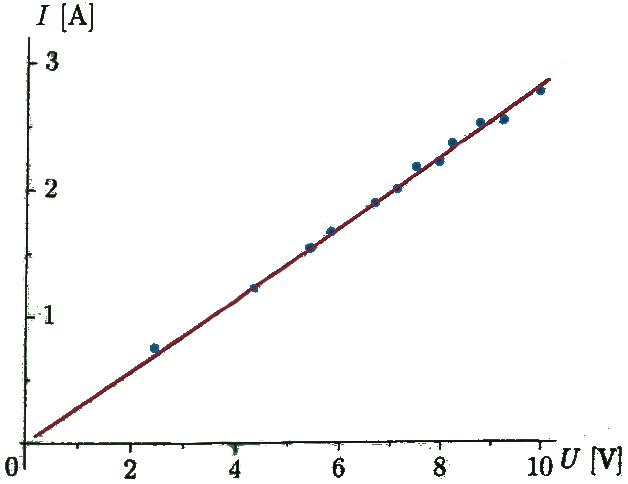
\includegraphics[width=0.8\linewidth]{mai_fig052.png}
  \captionof{figure}{Ověření Ohmová zákona lineární regresí.
  \cite[s.~263]{Musilova2009MA1}
  \label{mai:fig052}}
  \par}
  Pro odpor vychází \(R\doteq\SI{3.52}{\ohm}\). Součet čtverců odchylek přímky se směrnicí \(i/R
  = (1/\num{3.52})\Omega^{-1}\) od souboru bodů grafu je
  \begin{equation*}
    D(R) = \sum_{i=1}^{n}(U_i - R\cdot I_i)^2 \doteq\num{0.01},
  \end{equation*}
  \(\sigma(R) = \sqrt{D(R)/(n-1)}\doteq\sqrt{(\num{0.11}/11)}\doteq\num{0.03}\).  Graf přímky \(U
  = R\cdot I = \num{3.52}\cdot I\) proložené body je na obrázku \ref{mai:fig052}.
\end{mathexam}
      %---------------------------------------------------------------
      
      Popsaný způsob nalezení hodnoty elektrického odporu vodiče v příkladu \ref{mai:exam076} se
      nazývá\textbf{ metodou nejmenších čtverců} (minimalizuje součet čtverců odchylek prokládané
      závislosti od souboru naměřených bodů), v případě použití lineárního modelu, jako tomu bylo u
      Ohmová zákona, pak jde o \textbf{lineární regresi}
      
      Obdobně se postupuje, je-li některá z měřených veličin lineární funkcí veličin jiných s 
      neznámými koeficienty lineární kombinace. Nechť
      \begin{equation*}
        Z = f(X_1, X_2, \ldots, X_K) = A_1X_1 + A_2X_2 + \cdots + A_KX_K.
      \end{equation*}
      Předpokládejme, že veličiny \(X_1, X_2, \ldots, X_K\) a \(Z\) měříme \(n\)-krát a naměříme 
      hodnoty
      \begin{equation*}
        X_j = \lbrace x_{j1}, \ldots x_{jn} \rbrace, \; 1 \leq j \leq K, \; 
        Z = \lbrace z_{1}, \ldots z_{n} \rbrace
      \end{equation*}
      Součet čtverců odchylek teoretické závislosti od naměřených bodů je
      \begin{equation*}
        D(Z) = \sum_{i=1}^{n}\left(z_i - \sum_{j=1}^{K}A_jx_{ji}\right)^2.
      \end{equation*}
      Nutnou podmínkou pro minimum tohoto výrazu jakožto funkce proměnných \(A_x, A_2, \ldots, A_K\)
      je platnost souboru rovnic
      \begin{equation*}
        \pder{D(Z)}{A_p} = 0 \Rightarrow 
        \sum_{i=1}^{n}2\left(z_i - \sum_{j=1}^{K}A_jx_{ji}\right)\cdot x_{pi} = 0
      \end{equation*}
      pro \(1 \leq i \leq n, 1 \leq j \leq K\). Tyto podmínky představují nehomogenní soustavu 
      \(K\) rovnic pro \(K\) neznámých \(( A_1, A_2, \ldots, A_K)\). Rozšířená matice soustavy je
      \begin{strip}
      \begin{equation*}
        \overline{B} = (A\lvert B) = 
          \left(
            \begin{array}{cccc|c}
              \sum_{i=1}^{n}x_{1i}x_{1i} & \sum_{i=1}^{n}x_{1i}x_{2i} & \cdots & 
              \sum_{i=1}^{n}x_{1i}x_{Ki} & \sum_{i=1}^{n}z_{i}x_{1i}                    \\
              \sum_{i=1}^{n}x_{1i}x_{1i} & \sum_{i=1}^{n}x_{2i}x_{2i} & \cdots & 
              \sum_{i=1}^{n}x_{2i}x_{Ki} & \sum_{i=1}^{n}z_{i}x_{2i}                    \\
                        \cdots           & \cdots & \cdots & \cdots   & \cdots          \\
              \sum_{i=1}^{n}x_{Ki}x_{1i} & \sum_{i=1}^{n}x_{Ki}x_{2i} & \cdots & 
              \sum_{i=1}^{n}x_{Ki}x_{Ki} & \sum_{i=1}^{n}z_{i}x_{Ki}                    \\
            \end{array}
          \right),
      \end{equation*}
      \end{strip}
      \begin{equation*}
        \sigma(z) = \sqrt{\dfrac{D(z)}{n - K}}.
      \end{equation*}
      V dalších kapitolách věnovaných lineární algebře se k tomuto problému znovu vrátíme a ukážeme,
      že jej lze elegantně řešit také jako úlohu algebraickou, konkrétně úlohu o ortogonální
      projekci vektorů na podprostory.
      
%} %tikzset
%---------------------------------------------------------------------------------------------------


  % % !TeX spellcheck = cs_CZ
%{\tikzset{external/prefix={tikz/MAI/}}
% \tikzset{external/figure name/.add={ch10_}{}}
%---------------------------------------------------------------------------------------------------
% file mai1ch03.tex
%---------------------------------------------------------------------------------------------------
\chapter{Kombinatorika, pravděpdobnost, statistika}\label{mai:IchapIII}
\minitoc
  \section{Kombinatorika}\label{mai:IchapIIIsecI}
    \textbf{Kombinatorika} se od všech matematických disciplín, v několika směrech liší. Zatímco v 
    geometrii má každá přímka nekonečnou délku a každý trojúhelník nekonečně mnoho bodů, zatímco v 
    algebře některé rovnice i nerovnice mají nekonečně mnoho řešení a zatímco matematická analýza 
    zkoumá limity posloupností a funkcí, roste-li příslušná proměnná do nekonečna, v kombinatorice 
    se s nekonečnem nesetkáme. Kombinatorika je součástí \textbf{finitní matematiky}, která studuje 
    konečné soubory (množiny a uspořádané \(k\)-tice, \(k\in \mathcal{N}\)). 
    
    Další odlišností je to, že často nemáme možnost ověřit si správnost výsledku, ke kterému jsme 
    při řešení kombinatorické úlohy dospěli, a jsme odkázáni jen na svůj vlastní úsudek. Proto v 
    kombinatorice v míře větší než jinde platí, že „cvičení dělá mistra“. 
    
    V této kapitole je probrána část kombinatoriky, která se zabývá vytvářením skupin z daných 
    prvků a určováním jejich počtu. Jde o klasickou problematiku, která byla řešena již v 17. a 18. 
    století a která je spojena se jmény \emph{B. Pascala}, \emph{P. Fermata}, \emph{J Bernoulliho}, 
    \emph{G. W. Leibnize}  a \emph{L. Eulera}. Dnes představuje kombinatorika rozsáhlou 
    matematickou disciplínu, některé její problémy byly již vyřešeny (problém čtyř barev) mnohé 
    další na své vyřešení čekají. 
    
    A závěrem ještě důležitá poznámka terminologická: přirozeným čísly se v této kapitole rozumějí 
    čísla celá kladná tj. čísla 1, 2, 3, 4, \(\ldots\), nula se tedy mezi přirozená čísla 
    nezahrunuje. \cite[s.~7]{calda2008matematika} 
    
    \subsection{Základní kombinatorická pravidla}
    
    
    \cite[s.~7]{polak1991matematika}
    
  \section{Pravděpodobnost}\label{mai:IchapIIIsecII}
    Slovo pravděpodobnost používáme velmi často. Jaký však je jeho přesný význam? Jsme přesvědčeni, 
    že pravděpodobnost výhry ve sportce je velmi malá. Ani pravděpodobnost, že se vyplní předpověď 
    počasí, nepovažujeme mnohdy za výraznou. Přesto je mezi oběma příklady obrovský kvantitativní 
    rozdíl. Zkusme význam pojmu pravděpodobnost ukázat pomocí konkrétních číselných příkladů.
  
    \begin{itemize}
      \item \textbf{Příklad se střelcem}: Sportovní střelec střílí na terč série \num{100} ran. 
            Předpokládejme, že podmínky při střelbě jsou stále stejné. Stejná je zbraň, terč, 
            vzdálenost, povětrnostní podmínky i momentální zdravotní stav střelce. Při hodnocení 
            střelcova „mistrovství“ někdo řekne, že střelec zasáhne terč s pravděpodobností 
            \num{92}\%. Jak tomu rozumět? Znamená to, že v souboru sérií výstřelů jsou velmi časté 
            ty, v nichž zasáhl střelec terč \num{92}-krát. Samozřejmě, není řídké, že se objeví i 
            série s \num{93} nebo \num{94} zásahy, ale také s \num{91} nebo \num{90}. Vyloučen není 
            ani případ s úspěšností \num{96} či \num{88}, a dokonce i stovku bychom mohli 
            zaznamenat. Situace výrazně odlišné od \num{92} zásahů však budou řídké, a to tím více, 
            čím více se úspěšnost série liší od \num{92} oběma směry.
      \item \textbf{Příklad se zmetky}: Koupíte si výrobek u firmy, o které je známo, že vyrábí 
            zmetky s pravděpodobností 0,16\%? Situaci lze posuzovat obdobně jako úspěšnost střelce. 
            Budeme-li například zkoumat série obsahující 1000 výrobků, bude každá z nich obsahovat 
            „v průměru“ 16\% zmetků. Z příkladu se střelcem již zhruba víme, jak posuzovat slovo v 
            průměru.
    \end{itemize}
    
    V této kapitole se budeme pravděpodobnostmi zabývat podrobněji. Zjistíme, že i když se týkají 
    náhodných jevů, platí i pro ně jisté zákonitosti. V úvodních příkladech jsme si vyložili, jak 
    intuitivně chápat pojem pravděpodobnost. Jednalo se v nich o posouzení průměrné úspěšnosti ve 
    velkém souboru operací či úkonů prováděných za stejných podmínek, šlo tedy o jakousi 
    „průměrnou“ pravděpodobnost. Nyní definujeme pravděpodobnost matematicky.
    
    \subsection{Co se pravdě podobá - definice pravděpodobnosti}
      Pro definici pravděpodobnosti použijeme pojmu \emph{náhodný pokus}, jehož význam si ukážeme 
      na příkladu. Dobrým příkladem náhodných pokusů je třeba házení mincí, hraní kostkou, výběr 
      karet z balíčku, vidíme-li pouze jejich rub, apod. Budeme třeba házet kostkou. Abychom si 
      situaci zbytečně nekomplikovali, budeme předpokládat, že všechny výsledky hodu kostkou 
      (náhodné pokusy) jsou stejně časté, žádný z nich není nijak preferován\footnote{Kostka by 
      tedy měla být homogenní, plocha, na kterou po hodu dopadne, vodorovná, kvalita povrchu všech 
      stěn kostky stejná (žádná stěna by třeba neměla být natřena lepidlem), apod.}. Počet možných 
      výsledků jednotlivého hodu je \(N = 6\) (kostka má \num{6} stěn, na každé je vyznačen odlišný 
      počet ok, tedy \num{1} až \num{6}). Jednotlivé situace, které mohou nastat, nazýváme 
      náhodnými jevy. Náhodným jevem \(A\) tak může být situace \emph{„padne číslo \num{2}“}, jiným 
      náhodným jevem \(B\) situace \emph{„padne číslo dělitelné třemi“}, apod. Počet situací, kdy 
      výsledek hodu lze hodnotit tak, že určitý jev nastal, označíme \(M\). Například pro jev \(A\) 
      \emph{„padne číslo \num{2}“} je \(M(A)= 1\), pro jev \(B\) \emph{„padne číslo dělitelné 
      třemi“} je \(M(B) = 2\) (počet ok \num{3} nebo \num{6}). Můžeme také definovat jev \(O\) 
      \emph{„nepadne žádné číslo“} (\(M(0) = 0\)) nebo jev \(J\) \emph{„padne jakékoli číslo“} 
      (\(M(J) = 6\)).
      
      \begin{definition}
        Pravděpodobností jevu rozumíme podíl
        \begin{equation}\label{mai:eq011}
          p = \frac{M}{N} = \frac{\text{počet případů příznivých}}{\text{počet případů možných}}.
        \end{equation}  
        Počtem případů možných jsme zkráceně nazvali počet všech možných výsledků náhodného 
        pokusu, počtem případů příznivých pak počet všech takových výsledků pokusu, při nichž daný 
        jev nastal.
      \end{definition}
      Je zřejmé, že hodnota pravděpodobnosti jakéhokoli jevu je nezáporná a může nabývat hodnoty 
      nejvýše \num{1}, tj. \(0 <p< 1\). Jev s \emph{nulovou pravděpodobností} se nazývá 
      \textbf{nemožný}, jev s \emph{jednotkovou pravděpodobností} je \textbf{jistý}. V našem 
      příkladu s kostkou tak dostáváme
      \begin{equation*}
        p(A) = \frac{1}{6}, \qquad p(B) = \frac{2}{6} = \frac{1}{3}, \qquad
        p(O) = 0, \qquad p(J) = 1.
      \end{equation*}  

      %--Barevné ponožky----------------------------------------------
      % !TeX spellcheck = cs_CZ
\begin{example}
 \label{mai:exam006}
  \textbf{Barevné ponožky}:\newline\small
  V zásuvce jsou ponožky tří barev. Červené (\textbf{Č}), zelené (\textbf{Z}) a modré (\textbf{M}). 
  Je jich tam od každé barvy hodně. Student jde na schůzku a chce si vzít čisté ponožky. Náhle 
  zhasne světlo. Student vytáhne potmě dvě ponožky. Jaká je pravděpodobnost, že ponožky budou mít 
  stejnou barvu? Vyjmenujme případy, které mohou při vytažení dvou ponožek nastat: (\textbf{Č+Č}), 
  (\textbf{Č+Z}), (\textbf{Z+Č}), (\textbf{Č+M}), (\textbf{M+Č}), (\textbf{Z+Z}), (\textbf{Z+M}), 
  (\textbf{M+Z}), (\textbf{M+M}). Je tedy \(n = 9\). Příznivé situace jsou tří, (\textbf{Č+Č}), 
  (\textbf{Z+Z}), (\textbf{M+M}). Pravděpodobnost je tedy 1/3. (Převzato z 
  \cite[s.~200]{Musilova2009MA1}) 
\normalsize
\end{example}
      %---------------------------------------------------------------
    \subsection{Cifry, kostky, karty - kombinatorické opakování}
      Příklad s ponožkami byl velmi jednoduchý. Podařilo se nám vyjmenovat všechny případy možné i 
      všechny případy příznivé, neboť obojího bylo docela málo. Daleko běžnější jsou však situace, 
      kdy výčet případů není schůdný. A tehdy potřebujeme \textbf{kombinatoriku}.
      
      Nechť \(\mathcal{M}\) je \(n\)-prvková množina, z níž budeme provádět výběry \(k\) prvků 
      podle určitých pravidel. Prvky množiny \(\mathcal{M}\) nemusíme nijak konkretizovat. Abychom 
      si však o výběrech a pravidlech pro jejich tvorbu dokázali udělat nějakou názornou představu, 
      je taková konkretizace vhodná. Prvky množiny \(\mathcal{M}\): mohou být třeba žáci ve třídě, 
      barvy, hrací karty, apod. Výběry mohou představovat třeba družstva pro odbíjenou, signály 
      tvořené barevnými praporky, možnosti rozdání karet při mariáši, apod. Jednotlivé typy výběrů 
      získaly své názvy právě na základě pravidel stanovených pro jejich vytváření. Rozhodující 
      jsou dvě základní kritéria:
      \begin{itemize}\addtolength{\itemsep}{-0.5\baselineskip}
        \item Je pro tvorbu výběru podstatné pořadí prvků ve výběru či nikoliv?
        \item Mohou se prvky ve výběru opakovat či nikoliv?
      \end{itemize}
      
      Typy výběrů shrnuje následující diagram:
      \begin{figure}[ht!] %\ref{mai:fig021}
        \centering
        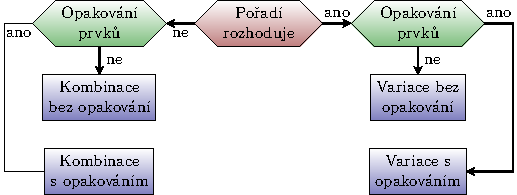
\includegraphics[width=0.7\linewidth]{mai_fig021.pdf}
        \caption{Typy výběrů. \cite[s.~201]{Musilova2009MA1}}
        \label{mai:fig021}
      \end{figure}

      Představuje-li daný výběr například volejbalové družstvo osmi děvčat (šest hráček a dvě 
      náhradnice), které bude reprezentovat v soutěži třídu osmou bé, do níž chodí \num{25} děvčat 
      a \num{18} chlapců, jedná se o výběr \(k - 8\) prvků z počtu \(n = 25\) prvků. Chlapce nelze 
      postavit do družstva volejbalistek. Každý výběr možného družstva bude představovat 
      \emph{kombinaci bez opakování}, neboť pořadí hráček nehraje roli a třeba Aničku Novákovou 
      máme ve třídě jen jednu. Budeme-li však chtít vytvářet z deseti cifer \(0, 1, \ldots, 9\) 
      trojciferná čísla, pak tyto výběry tří prvků z deseti (\(k = 3\), \(n = 10\)) jsou 
      \emph{variacemi s opakováním}. Čísla \num{125}, \num{512}, \num{251}, \num{215}, \num{521} a 
      \num{152} jsou totiž různá, a například \num{222} je také trojciferné číslo. Kombinace s 
      opakováním bychom mohli vytvářet třeba i při výběru různobarevných ponožek ze zásuvky a 
      konečně \emph{variacemi bez opakování} by mohly být dejme tomu trojbarevné signály (\(k = 
      3\)) tvořené trojicemi barevných hadříků vybíraných z \(n\) barev (pro \(n = 3\) třeba zrovna 
      z těch ponožek). Nyní bychom však rádi věděli, jak pro zadané hodnoty \(n\) a \(k\) určit 
      počet všech možných výběrů předepsaného typu. Ukážeme si to na příkladech.

      %--Šance milion-------------------------------------------------
      % !TeX spellcheck = cs_CZ
\begin{mdframed}[style=mdexam]
  \begin{example}\label{mai:exam007}
    \textbf{Šance milion}:\newline
    „Znáte nějakou jinou hru, kde můžete denně vyhrát milion?“ Tento nebo jiný, obdobně nepříliš
    vtipný reklamní slogan propaguje v televizi hru, jejímž cílem je uhodnout šestici tažených cifer
    ve správném pořadí. (Hru raději nehrajte, pravděpodobnost výhry je mizivá.) Tah se provádí
    následovně: V každém ze šesti bubnů, očíslovaných pořadovými čísly \num{1} až \num{6}, je
    připraveno deset míčků opatřených ciframi \(0, 1, \ldots, 9\). Z prvního bubnu se náhodně
    vylosuje jedna cifra (deset možností). Poté se náhodně vylosuje jedna cifra z druhého bubnu
    (opět deset možností). Možností vzniku uspořádané dvojice cifer (jedna cifra z prvního a druhá z
    druhého bubnu) je již sto (každou možnost výsledku u prvního bubnu lze kombinovat s každou
    možností výsledku z druhého bubnu). Losování pokračuje u třetího, čtvrtého, pátého a šestého
    bubnu. Celkový počet možností je \num{1e6}, tedy \textbf{milion}. (Šance získat výhru, tedy
    vyhrát milion, je ovšem pouze jedna milióntina, neboť z milionu možností je pouze jedna skutečně
    tažena.) 
  \end{example}
\end{mdframed}
      %---------------------------------------------------------------
      
      Zobecněním předchozího příkladu získáváme vzorec pro počet \textbf{variací s opakováním} 
      \emph{k}-té třídy z \(n\) prvků. Při tahu totiž záleží na pořadí bubnů a každý buben obsahuje 
      všechny cifry. Výsledky tahů z jednotlivých bubnů se tedy mohou opakovat. Pokud by bubnů bylo 
      \(k\) a v každém \(n\) různých cifer, dostali bychom pro \textbf{variace s opakováním 
      \(k\)-té třídy z \(n\) prvků} celkový počet
      \begin{equation}\label{mai:eq007}
        \boxed{V_k' = n^k}\, .
      \end{equation}

      %--Modifikovaná šance milion------------------------------------
      % !TeX spellcheck = cs_CZ
\begin{example}\label{mai:exam008}
  \textbf{Modifikovaná šance milion}:\newline
  Představme si hru z předchozího příkladu upravenou takto: K dispozici bude jen jeden buben s 
  ciframi \(0, 1, \ldots, 9\), každá cifra je v bubnu obsažena pouze jednou. Opět máme losovat 
  uspořádanou \textbf{šestici cifer}. Nyní se však jedná o \textbf{variace šesté třídy z deseti 
  prvků bez opakování}. S jediným bubnem musíme totiž provést šest losování, přičemž při každém 
  losování ubude z bubnu jedna cifra. Při prvním tahu je deset možností, při druhém již jen devět, 
  atd., při šestém již pouze pět možností. Celkem je tedy \(10 \cdot 9 \cdots 5 = \num{151200}\) 
  možností.
\end{example}
      %---------------------------------------------------------------
      
      Uvážíme-li, že v předchozím příkladu je \(n = 10\) a \(k = 6\), dostáváme pro \textbf{počet 
      variací bez opakování \(k\)-té třídy z \(n\) prvků} obecný vztah
      \begin{align}
        V_k(n) &= n(n-1)(n-2)\cdots(n-k+1)  \nonumber \\
        \shortintertext{neboli}
        V_k(n) &= \frac{n!}{(n-k)!}\, .    \label{mai:eq008}
      \end{align}
      Poznamenejme, že \(n!\) značí \textbf{faktoriál}, \(n! = n(n - 1)\cdots 3 \cdot 2 \cdot 1\). 
      Pro nulu definujeme \(0! = 1\). Je zřejmé, že při vytváření variací bez opakování musí být 
      \(k\leqq n\). Variace bez opakování \(n\)-té třídy z \(n\) prvků se nazývají 
      \textbf{permutace}. Každá z nich představuje určité uspořádání těchto \(n\) prvků. Platí
      \begin{equation}\label{mai:eq009}
        \boxed{P(n) = V_n(n) = n!}\, .
      \end{equation}
      
      Nyní odvodíme vzorec pro počet \textbf{kombinací \(k\)-té třídy z \(n\) prvků bez opakování}. 
      Již jsme si řekli, že \emph{kombinací} rozumíme takový výběr z celkového počtu \(n\) prvků, 
      který obsahuje určitých \(k\) prvků nezávisle na jejich pořadí. Představme si, že máme k 
      dispozici všechny variace bez opakování \(k\)-té třídy ze zmíněných \(n\) prvků. Vezměme 
      kteroukoli z nich. Soubor všech variací \(k\)-té třídy z \(n\) prvků však obsahuje i další 
      variace, lišící se od té naší jen pořadím prvků. Celkem je takových variací (i s tou první) 
      \(k!\) a z hlediska kombinací představují totéž. Soubor variací se tak rozpadá na podsoubory, 
      z nichž každý obsahuje \(k!\) variací lišících se navzájem pouze pořadím prvků. Každý z 
      těchto podsouborů představuje však jedinou kombinaci. Počet kombinací \(k\)-té třídy z \(n\) 
      prvků bez opakování je tedy
      \begin{equation}\label{mai:eq010}
        \boxed{C(k) = \frac{V_k(n)}{P(k)} = \frac{n!}{(n-k)!\,k!} = 
               \begin{pmatrix}
                n \\
                k
               \end{pmatrix}}\, .
      \end{equation}
      
      Pro odvození vzorce pro \textbf{kombinace s opakováním} použijeme opět příkladu.
      %--Kuličky v přihrádkách----------------------------------------
      % !TeX spellcheck = cs_CZ
\begin{mathexam}{Kuličky v přihrádkách}{exam009}
  Máme kuličky \(n\) různých barev, v každé barvě máme tolik kuliček, kolik bude potřeba. Naším
  úkolem je vytvářet výběry \(k\) kuliček. Na \textbf{pořadí barev nezáleží}, kuliček jedné barvy
  může být ve výběru libovolný počet \(0\leqq s \leqq k\). Výběry budeme vytvářet tak, že budeme
  kuličky dávat do \(n\) přihrádek, z nichž každá bude vyhrazena pro určitou barvu. Pokud tedy v
  daném výběru zrovna nebude třeba modrá kulička, bude přihrádka vyhrazená pro modrou barvu prázdná.
  Budou-li v daném výběru právě tři červené kuličky, budou umístěny v přihrádce vyhrazené pro
  červenou barvu. Vidíme, že pokud konkrétním přihrádkám přisoudíme konkrétní barvy, samotné kuličky
  by již barevné být nemusely, stačily by třeba kuličky skleněné, bezbarvé. Zůstane-li například
  přihrádka pro modrou barvu prázdná, víme, že daný výběr neobsahuje modrou barvu. Budou-li v
  přihrádce pro červenou barvu tři (bezbarvé) kuličky, víme, že daný výběr obsahuje červenou barvu
  třikrát. Příklad takové situace ukazuje následující schéma:
  
  {\centering
    \luafigure[0.9]{mai_fig033.pdf}
    \par}

  Náš úkol můžeme přeformulovat takto: Je třeba rozmístit \(k\) kuliček do \(n\) přihrádek. V každé
  přihrádce může být obecně \(s\) kuliček, kde \(0\leqq s \leqq k\), přitom celkový počet kuliček
  musí být samozřejmě stále \(k\). Můžeme si představit, že \(k\) kuliček máme položených v řadě na
  polici mezi dvěma pevnými stěnami (krajní svislé čáry v předchozím schématu) a různé způsoby
  rozmístění kuliček do přihrádek provádíme přemísťováním pohyblivých přepážek. Kdybychom například
  v předchozím schématu přesunuli druhou svislou čáru, počítáno zleva, až za první kuličku v
  přihrádce na červenou barvu, dostaneme uspořádání, při němž je v přihrádce na modrou barvu jedna
  kulička a v přihrádce na červenou barvu dvě kuličky. Tedy takto:

  {\centering
    \luafigure[0.9]{mai_fig034.pdf}
  \par}

  Mezi dvěma krajními pevnými stěnami máme tedy k dispozici \(k\) pozic pro kuličky a \((n - 1)\)
  pozic pro pohyblivé přepážky. Celkem tedy \((n + k - 1)\) pozic, na které můžeme libovolně
  rozmísťovat \(k\) kuliček a \((n - 1)\) přepážek. Do těchto \((n + k - 1)\) pozic můžeme umístit
  \(k\) kuliček \(C_k'(n)\) způsoby, kde
  \begin{equation}\label{MAI:eq011}
    \boxed{C_k'(n) =  \binom{n + k - 1}{k} = \binom{n + k - 1}{n -1}}\, .
  \end{equation}
  Na zbylé pozice již musíme umístit přepážky. Nebo naopak, nejprve umístíme \((n - 1)\) přepážek a
  potom kuličky. Výsledek je stejný, jak je vidět z předchozího vzorce. Protože jsme vytváření
  kombinací s opakováním \(k\)-té třídy z \(n\) prvků převedli na úlohu o rozmísťování kuliček do
  přihrádek, udává získaný vzorec právě počet takových kombinací. Aby měl vzorec smysl, musí platit
  \(n + k - 1 \geqq k\), tedy \(n \geqq 1\).

  Komu nevyhovuje představa kuliček v přihrádkách a má raději čísla, může uvažovat následovně: Tak
  jako je každé číslo v desítkové soustavě zapsáno pomocí cifer \(0, 1, 2, \ldots , 8, 9\), je k
  jeho zápisu ve dvojkové soustavě potřeba pouze dvou cifer, nuly a jedničky. Představme si nyní
  přepážku jako jedničku a kuličku jako nulu. Náš úkol zjistit počet všech možných způsobů rozdělení
  \(k\) kuliček do \(n\) přihrádek, ohraničených \((n+1)\) přepážkami, můžeme převést na
  ekvivalentní problém: Kolik dokážeme najít čísel, která jsou ve dvojkové soustavě zapsána právě
  \(k\) nulami a \((n + 1)\) jedničkami, požadujeme-li, aby první i poslední cifrou byla jednička?
  Odpověď je jednoduchá. Máme k dispozici \((n+k+1)\) pozic pro cifry. První a poslední pozice jsou
  pevně obsazeny jedničkami, volných pozic je tedy pouze \((n + k - 1)\). Počet všech různých
  způsobů, kterými na \(k\) z těchto pozic můžeme umístit nuly, je roven počtu kombinací \(k\)-té
  třídy z \((n + k - 1)\) prvků. Na zbylé pozice již musíme umístit jedničky. Komplementárně,
  budeme-li hledat počet všech možných způsobů, jak na \((n-1)\) pozic umístit jedničky, dostaneme
  shodný výsledek, v souhlasu se vzorcem (\ref{mai:eq010}).
\end{mathexam}
      %---------------------------------------------------------------
      
      %--Obsazování kvantových stavů----------------------------------
      % !TeX spellcheck = cs_CZ
\begin{example}\label{mai:exam010}
  \textbf{Obsazování kvantových stavů}:\newline\small
  Úloha o kuličkách a přihrádkách má přímou aplikaci v \textbf{kvantové fyzice}. Představme si, že 
  fyzikální soustava je tvořena \(k\) částicemi. Každá částice se nachází v určitém stavu, v němž 
  jí můžeme přisoudit fyzikální charakteristiky, které jsou s tímto stavem spojeny (třeba energii, 
  moment hybnosti, apod.). Jednotlivé stavy jsou pak rozlišitelné právě pomocí těchto 
  charakteristik. Dejme tomu, že přípustných stavů je \(n \geqq 1\). Problémem kvantové fyziky je 
  to, že kvantové částice jsou nerozlišitelné. Nepoznáme jednu od druhé. Je to stejné, jako bychom 
  měli \(k\) naprosto stejně vypadajících kuliček, které nemáme nijak očíslovány. Záměna dvou 
  částic (nerozlišitelných kuliček) se nepozná, nevede tedy ke změně stavu fyzikální soustavy. Pro 
  hodnoty fyzikálních charakteristik soustavy jako celku je tedy důležité jen to, kolik částic je v 
  každém z přípustných stavů. Musíme se tedy zajímat o to, kolika způsoby lze našich \(k\) 
  \textbf{nerozlišitelných částic} (kuliček) umístit do \(n\) \textbf{stavů} (přihrádek). Kvantové 
  částice jsou však dvojího druhu, \textbf{fermiony} (například elektrony, neutrony, protony, jádra 
  s lichým počtem nukleonů) a \textbf{bosony} (například fotony, mezony, jádra se sudým počtem 
  nukleonů). Rozdíl mezi nimi je ten, že bosony se „dobře snášejí“, a proto jich může být v jednom 
  stavu i více. 
  \begin{itemize}\addtolength{\itemsep}{-0.5\baselineskip}
    \item Počet možností, jak rozmístit \(k\) \textbf{bosonů} po \(n\) stavech je tedy
          \begin{equation*}
            N_{\text{boson}} = 
              \begin{pmatrix}
                n + k - 1 \\
                    k
               \end{pmatrix}
          \end{equation*}
    \item S \textbf{fermiony} je tomu jinak. \textbf{Pauliho vylučovací princip} jim zakazuje, 
          aby v daném stavu byl více než jeden fermion. Stav může být buď prázdný, nebo obsazen 
          jedním fermionem. V takovém případě musí být \(n \geqq k\) a v každé přihrádce může být 
          nejvýše jedna kulička. Situace tak odpovídá \textbf{kombinacím bez opakování \(k\)-té 
          třídy z \(n\) prvků}, tj.
          \begin{equation*}
            N_{\text{fermion}} = 
              \begin{pmatrix}
                n  \\
                k
              \end{pmatrix}
          \end{equation*}
  \end{itemize}
\normalsize
\end{example}
      %---------------------------------------------------------------
      
      Získané kombinatorické vzorce nyní použijeme při řešení základních úloh o pravděpodobnostech. 
      V každé úloze bude důležité
      \begin{itemize}
        \item definovat jev \(A\), jehož pravděpodobnost počítáme,
        \item určit počet \(N\) případů možných, tj. počet všech možných výsledků pokusu, při 
              kterém sledujeme, zda jev \(A\) nastal či nenastal,
        \item určit počet \(M\) případů příznivých, tj. počet těch výsledků daného pokusu, při 
              kterých jev \(A\) nastal.
      \end{itemize}

      %--Výhra ve sportce---	----------------------------------------
      % !TeX spellcheck = cs_CZ
\wikitextrule
\begin{example}\label{mai:exam052}
  \textbf{Výhra ve sportce}\newline\small
  Jaká je pravděpodobnost hlavní výhry ve sportce? Všichni víme, že malá, ale máme představu, jak 
  malé toto číslo je? Při sportce se losuje \(k = 6\) čísel a jedno dodatkové z celkového počtu \(n 
  = 49\) čísel. (Dříve byla čísla spojena s názvy sportů, odtud název „sportka“ .) Na pořadí čísel 
  ve výběru nezáleží, vytažené číslo se do hry nevrací. Jde tedy o \textbf{kombinace bez 
  opakování}. Hlavní výhra požaduje uhodnout všech \num{6} tažených čísel. Jev \(A\) je tedy 
  definován takto:
  
  \begin{itemize}
    \item Jev \(A\): Bude taženo právě oněch \num{6} čísel, která jsem vsadil.
          Počet možností, které při tahu sportky mohou nastat (počet případů možných), je \(N = 
          \begin{pmatrix} n \\ k\end{pmatrix} =  \begin{pmatrix} 49 \\ 6 \end{pmatrix} \). Hlavní 
          výhru představuje jediná kombinace, počet příznivých případů je proto \(M = 1\). 
          Pravděpodobnost hlavní výhry ve sportce, tj. pravděpodobnost jevu \(A\), je
          \begin{equation*}
            p(A) = \dfrac{M}{N} = \dfrac{1}{\begin{pmatrix} 49 \\ 6 \end{pmatrix}} 
                 = \dfrac{43!6!}{49!} = \dfrac{720}{49\cdot48\cdot47\cdot46\cdot45\cdot44} \simeq 
                 \num{7e-8}
                 = \SI{7e-6}{\percent}
          \end{equation*}
          Pravděpodobnost hlavní výhry je velmi malá, sedm milióntin procenta. 
    \item A o kolik lepší to bude s pravděpodobností některé z vedlejších výher? Tak třeba pátá 
          cena znamená, že je nutné ze šesti tažených čísel uhodnout libovolné tři. Jev \(A\) je 
          tedy: Ze šesti čísel, která jsme vsadili, budou v tažené kombinaci obsažena právě tři 
          libovolná z nich. Počet \(N\) zůstává stejný jako v předchozí části úlohy. Je třeba jen 
          určit \(M\). Každý příznivý případ vzniká tak, že trojice správných čísel (výběry tří ze 
          šesti) je doplněna trojicí chybných čísel (výběry tří ze čtyřiceti tří). Tedy \(M = 
          \begin{pmatrix}6 \\ 3\end{pmatrix}\begin{pmatrix} 49 - 6 \\ 3\end{pmatrix} =  
          \begin{pmatrix} 6 \\ 3\end{pmatrix}\begin{pmatrix} 43 \\ 3 \end{pmatrix}\),
          \begin{align*}
            p(A) &= \dfrac{M}{N} 
                  = \dfrac{\begin{pmatrix} 6 \\ 3\end{pmatrix}
                           \begin{pmatrix} 43 \\ 3 \end{pmatrix}}
                          {\begin{pmatrix} 49 \\ 6\end{pmatrix} }                
                  =\left(\dfrac{6!}{3!\cdot3!}\right)\left(\dfrac{43!}{40!\cdot3!}\right)
                   \left(\dfrac{43!6!}{49!}\right)                                            \\
                 &=\dfrac{120\cdot43\cdot42\cdot41\cdot720}
                         {49\cdot48\cdot47\cdot46\cdot45\cdot44\cdot36} 
                  \simeq\num{0.018}.
          \end{align*}
          Tato pravděpodobnost již zanedbatelná není, na rozdíl od finanční částky, jíž bývá 
          ohodnocena pátá cena. Sázení sportky může domácímu rozpočtu spíše ublížit.
    \item Třetí, resp. čtvrtá cena jsou, podobně jako první a pátá, definovány velmi jednoduše. Je 
          třeba uhodnout pět, resp. čtyři ze šesti tažených čísel. V případě druhé ceny hraje roli
          dodatkové číslo. Druhou cenu získává ten, kdo uhodl pět ze šesti čísel vylosovaných v 
          prvním tahu a ještě navíc číslo dodatkové, které se losuje ze zbylých \num{43} čísel, jež 
          zůstala po prvním tahu v osudí. Jev \(A\) je tedy definován takto:
          
          Ze šesti čísel, která jsem vsadil, bude při prvním tahu vylosováno libovolných pět a v 
          druhém tahu bude vylosováno právě to dodatkové číslo, které jsem vsadil. Počet případů 
          příznivých je pouze \(M = \begin{pmatrix}6 \\ 5\end{pmatrix}\), neboť šestým číslem 
          nemůže být libovolné ze \num{43} čísel, která nebyla v prvním tahu vylosována, ale 
          musí to být právě číslo dodatkové. Pravděpodobnost jevu \(A\) je
          \begin{equation*}
            p(A)  = \dfrac{M}{N} 
                  = \dfrac{\begin{pmatrix} 6  \\ 5\end{pmatrix}}
                          {\begin{pmatrix} 49 \\ 6\end{pmatrix}}
                  \simeq\num{4.2e-17}.
          \end{equation*}
          
          Pokud bychom jako jev \(A\) označili výhru jakékoliv ceny, dostaneme
          \begin{align*}
            M &= \sum_{6}^{k=3}\begin{pmatrix} 6  \\   k  \end{pmatrix}
                               \begin{pmatrix} 43 \\ 6 - k\end{pmatrix}  +
                               \begin{pmatrix} 6  \\   5  \end{pmatrix}                      \\
              &= \begin{pmatrix} 6 \\ 3\end{pmatrix}\begin{pmatrix} 43 \\ 3\end{pmatrix} +
                 \begin{pmatrix} 6 \\ 4\end{pmatrix}\begin{pmatrix} 43 \\ 2\end{pmatrix} +
                 \begin{pmatrix} 6 \\ 5\end{pmatrix}\begin{pmatrix} 43 \\ 1\end{pmatrix} +
                 \begin{pmatrix} 6 \\ 6\end{pmatrix}\begin{pmatrix} 43 \\ 0\end{pmatrix} +
                 \begin{pmatrix} 6 \\ 5\end{pmatrix},                                        \\
           p(A) &= \dfrac{\begin{pmatrix}  6 \\ 3\end{pmatrix}
                          \begin{pmatrix} 43 \\ 3\end{pmatrix}  +
                          \begin{pmatrix}  6 \\ 4\end{pmatrix}
                          \begin{pmatrix} 43 \\ 2\end{pmatrix}  +
                          \begin{pmatrix}  6 \\ 5\end{pmatrix}
                          \begin{pmatrix} 43 \\ 1\end{pmatrix}  +
                          \begin{pmatrix}  6 \\ 6\end{pmatrix}
                          \begin{pmatrix} 43 \\ 0\end{pmatrix}  +
                          \begin{pmatrix}  6 \\ 5\end{pmatrix}}
                         {\begin{pmatrix} 49 \\ 6\end{pmatrix}} =\simeq\num{0.019}.
          \end{align*}
          Všimněte si, že tento výsledek je roven součtu pravděpodobností výhry páté, čtvrté, 
          třetí, druhé a hlavní ceny. Později si tento závěr ještě připomeneme.
  \end{itemize}  
  \normalsize
\end{example}
      %---------------------------------------------------------------

      %--Losování karet-----------------------------------------------
      % !TeX spellcheck = cs_CZ
\wikitextrule
\begin{example}\label{mai:exam053}
  \textbf{Losování karet}\newline\small
    Máme karetní hru mariáš, která obsahuje celkem \num{32} karet osmi hodnot \num{7}, \num{8}, 
    \num{9}, \num{10}, J (kluk), Q (dáma), K (král), A (eso), každá hodnota je ve čtyřech barvách, 
    červené barvy jsou \(\heartsuit\) (srdce) a \(\lozenge\) (kára), černé barvy jsou \(\spadesuit\)
    (piky) a \(\clubsuit\) (kříže). Jaká je pravděpodobnost, že při náhodném vylosování deseti 
    karet budou 
    mezi nimi:
    \begin{enumerate}[label=\Alph*]
      \item právě dvě esa,
      \item alespoň dvě esa,
      \item nejvýše dvě esa,
      \item alespoň šest karet stejné barvy,
      \item právě dvě dámy a alespoň jeden kluk,
      \item právě dvě dámy nebo alespoň jeden kluk?
    \end{enumerate}

    Písmena (A) až (F) představují různé části úlohy a také zároveň definují jevy, jejichž 
    pravděpodobnost počítáme. Jedná se opět o kombinace. Nezáleží totiž na pořadí, v jakém karty 
    vytahujeme. Důležité je jen to, zda jsou vyjmenované karty ve výběru obsaženy. Počet možných 
    výsledků náhodného vylosování deseti karet z dvaatřiceti, tj. počet případů možných, je pro 
    všechny části úlohy stejný,
    \begin{equation*}
      N = \begin{pmatrix} 32 \\ 10\end{pmatrix} 
        = \dfrac{32\cdot31\cdots24\cdot23}{10\cdot9\cdots2\cdot1} = \num{64512240}.
    \end{equation*}
    
    Počítejme nyní případy příznivé pro jednotlivé jevy \(A\) až \(F\) a pravděpodobnosti těchto 
    jevů:
    \begin{equation*}
      M(A) = \begin{pmatrix} 4 \\ 2\end{pmatrix}\begin{pmatrix} 32 - 4 \\ 10 - 2\end{pmatrix}
           = \begin{pmatrix} 4 \\ 2\end{pmatrix}\begin{pmatrix} 28 \\ 8\end{pmatrix}
           = 6\cdot\dfrac{28\cdot27\cdots1}{8\cdot7\cdots2\cdot1} = \num{18648630}.
    \end{equation*}
    Jak jsme k tomuto výsledku došli? Příznivý pro daný jev je každý výběr, v němž jsou obsažena 
    právě dvě esa (libovolných barev) a žádná další esa (význam slova „právě“). Počet výběrů dvou 
    es z celkového počtu čtyř es je \(C_2(4)\), počet výběrů dalších libovolných osmi karet ze 
    zbývající části hry, která vznikne po odstranění es (nechceme, aby v příznivém výběru byla 
    další esa), je \(C_{(10-2)}(32 - 4) = C_8(28)\). Každý výběr dvojice es lze kombinovat s každým 
    výběrem zbývajících osmi karet ze zbytku hry, tj. \(M(A) = C_2(4)\cdot C_8(28)\). A to je právě
    náš předchozí výsledek. Potom:
    \begin{equation*}
      p(A) = \dfrac{M(A)}{N} 
           = \dfrac{\begin{pmatrix} 4 \\ 2\end{pmatrix}\begin{pmatrix} 28 \\ 8\end{pmatrix}}
                   {\begin{pmatrix} 32 \\ 10\end{pmatrix}}
           = \dfrac{\num{18648630}}{\num{64512240}} \simeq \num{0.29}
    \end{equation*}
    
    Aby nastal jev \(B\), požadujeme, aby v náhodném výběru deseti karet z dvaatřiceti byla alespoň 
    dvě esa. To znamená, že výběr považujeme za příznivý, obsahuje-li dvě esa libovolné barvy a osm 
    libovolných karet jiné hodnoty, nebo obsahuje tři esa libovolné barvy a sedm libovolných karet 
    jiné hodnoty, nebo obsahuje všechna čtyři esa a šest libovolných karet jiné hodnoty, \(k\) es 
    (pro \(k = 2, 3, 4\)) můžeme ze čtyř es vybrat \(\begin{pmatrix} 4 \\ k\end{pmatrix}\) způsoby.
    \(10 - k\) karet jiné hodnoty pak musíme vybírat pouze z \num{28} karet (esa je nutno 
    odstranit, aby bylo zaručeno, že „doplňkové“ karty budou mít jinou hodnotu než eso). Výběr 
    zbývajících karet lze učinit \(\begin{pmatrix} 28 \\ 10 - k\end{pmatrix}\) způsoby. Nakonec 
    tedy dostáváme
    \begin{align*}
      M(B) &=  \begin{pmatrix} 4 \\ 2\end{pmatrix}\begin{pmatrix} 28 \\ 8\end{pmatrix}
              +\begin{pmatrix} 4 \\ 3\end{pmatrix}\begin{pmatrix} 28 \\ 7\end{pmatrix}
              +\begin{pmatrix} 4 \\ 4\end{pmatrix}\begin{pmatrix} 28 \\ 6\end{pmatrix}         \\
           &=  6\cdot\dfrac{28\cdot27\cdots22\cdot21}{8\cdot7\cdots2\cdot1}
              +4\cdot\dfrac{28\cdot27\cdots23\cdot22}{7\cdot6\cdots2\cdot1}
              +1\cdot\dfrac{28\cdot27\cdots24\cdot23}{6\cdot5\cdots2\cdot1} = \num{23761530},  \\
      P(B) &= \dfrac{M(B)}{N} = \dfrac{\num{23761530}}{\num{64512240}} \simeq\num{0.37}.
    \end{align*}
    Pozn.: Někomu se předchozí výpočet může zdát příliš složitý. Nelze jej nějak zjednodušit? Co 
    kdybychom uvažovali třeba takto: Výběr dvou es již zajistí splnění požadavku. Doplňkové karty 
    tedy již pak můžeme vybírat ze třiceti karet - nebudeme tedy odstraňovat esa, protože budou-li 
    vybrána mezi doplňkovými kartami, požadavek „alespoň dvou es ve výběru“ to nenaruší. Při takové 
    interpretaci bychom dostali
    \begin{equation*}
      M(B) = \begin{pmatrix} 4 \\ 2\end{pmatrix}\begin{pmatrix} 30 \\ 8\end{pmatrix}   
           = 6\cdot\dfrac{30\cdot29\cdots24\cdot23}{8\cdot7\cdots2\cdot1}
           = \num{35117550}.
    \end{equation*}
    Vidíme, že vyšlo číslo vyšší než při předchozí úvaze. Co je tedy správně? Správně je první 
    úvaha vedoucí k nižšímu počtu příznivých případů. Při druhé úvaze jsme některé případy 
    započetli vícekrát. Zkuste přijít na to, jak se to stalo. V každém případě vidíme, že 
    kombinatorické úvahy, ať již vypadají jakkoli jednoduše, mohou být zrádné a je třeba dát si na 
    ně pozor. 
    
    Jev \(C\) podle zadání nastane, obsahuje-li náhodný výběr deseti karet nejvýše dvě esa. Znamená 
    to, že výběr je příznivý, neobsahuje-li žádné eso a obsahuje deset karet jiné hodnoty, nebo 
    obsahuje-li jedno eso a devět karet jiné hodnoty, nebo obsahuje-li dvě esa a osm karet jiné 
    hodnoty. Počet \(M(C)\) určíme analogicky jako \(M(B)\), ale pro \(k= 0, 1, 2\):
    \begin{align*}
      M(C) &=  \begin{pmatrix} 4 \\ 0\end{pmatrix}\begin{pmatrix} 28 \\ 10\end{pmatrix}
              +\begin{pmatrix} 4 \\ 1\end{pmatrix}\begin{pmatrix} 28 \\ 9\end{pmatrix}
              +\begin{pmatrix} 4 \\ 2\end{pmatrix}\begin{pmatrix} 28 \\ 8\end{pmatrix}         \\
           &=   \cdot\dfrac{28\cdot27\cdots20\cdot19}{10\cdot9\cdots2\cdot1}
              +4\cdot\dfrac{28\cdot27\cdots21\cdot20}{ 9\cdot8\cdots2\cdot1}
              +6\cdot\dfrac{28\cdot27\cdots22\cdot21}{ 8\cdot7\cdots2\cdot1} = \num{59399340}, \\
      P(C) &= \dfrac{M(C)}{N} = \dfrac{\num{59399340}}{\num{64512240}} \simeq\num{0.92}.
    \end{align*}
    
    Jev \(D\) znamená alespoň šest karet stejné barvy (připomeňme, že barvou rozumíme jednu z 
    možností \(\heartsuit\), \(\lozenge\), \(\spadesuit\), \(\clubsuit\)). Hra obsahuje osm karet 
    od každé barvy. Současně je tedy zřejmé, že karet stejné barvy může být ve výběru nejvýše osm. 
    Výběr je příznivý pro \(k = 6, 7, 8\). Obdobnou úvahou jako v předchozích případech dostáváme
    \begin{equation*}
      M = 4\cdot\sum^{8}_{k=6}
          \begin{pmatrix} 8 \\ k \end{pmatrix}\begin{pmatrix} 32 - 8 \\ 10 - k\end{pmatrix}
        = \num{1255984}.
    \end{equation*}
    
    Faktor \num{4} před celou sumou se objevuje proto, že nebylo specifikováno, která ze čtyř barev 
    má být zastoupena alespoň šesti kartami. Všechny čtyři možnosti volby barvy jsou tedy příznivé. 
    Pravděpodobnost jevu \(D\) je
    \begin{equation*}
      p(D)  = \dfrac{M(D)}{N}
            = \dfrac{4\cdot\sum^{8}_{k=6}\dfrac{8!}{k!(8-k)!}\dfrac{24!}{(10-k)!(14+k)!}}
                    {\begin{pmatrix} 32 \\ 10 \end{pmatrix}}                               
            = \dfrac{\num{1255984}}{\num{64512240}} \simeq \num{0.019}.
    \end{equation*}
    
    Případy (\(E\)) a (\(F\)) v zadání se liší pouze slůvkem „a“ a „nebo“. Uvidíme, že nejde o 
    slovíčka, ale o podstatný rozdíl. 
    
    Aby nastal jev \(E\), požadujeme, aby náhodný výběr deseti karet obsahoval právě dvě dámy a 
    alespoň jednoho kluka. Znamená to, že výběr je příznivý, obsahuje-li dvě dámy libovolné barvy a 
    současně alespoň jednoho kluka libovolné barvy. Příznivé možnosti tedy jsou:
    \begin{enumerate}
    \item  dvě dámy libovolné barvy, jeden kluk libovolné barvy, \num{7} libovolných karet, které 
           nemají hodnotu dámy ani kluka, celkem 
           \(\begin{pmatrix} 4 \\ 2 \end{pmatrix}
             \begin{pmatrix} 4 \\ 1\end{pmatrix}
             \begin{pmatrix} 32-2\cdot4 \\ 7 \end{pmatrix} = \num{8306496}\) možností,
    \item dvě dámy libovolné barvy, dva kluci libovolné barvy, \num{6} libovolných karet, které 
          nemají hodnotu dámy ani kluka, celkem 
          \(\begin{pmatrix} 4 \\ 2 \end{pmatrix}
            \begin{pmatrix} 4 \\ 2\end{pmatrix}
            \begin{pmatrix} 32-2\cdot4 \\ 6 \end{pmatrix} = \num{4845456}\) možností,
    \item dvě dámy libovolné barvy, tři kluci libovolné barvy, \num{5} libovolných karet, které 
          nemají hodnotu dámy ani kluka, celkem 
          \(\begin{pmatrix} 4 \\ 2 \end{pmatrix}
            \begin{pmatrix} 4 \\ 3\end{pmatrix}
            \begin{pmatrix} 32-2\cdot4 \\ 5 \end{pmatrix} = \num{1020096}\) možností,
    \item dvě dámy libovolné barvy, všichni čtyři kluci, \num{4} libovolné karty, které nemají 
          hodnotu dámy ani kluka, celkem 
          \(\begin{pmatrix} 4 \\ 2 \end{pmatrix}
            \begin{pmatrix} 4 \\ 4\end{pmatrix}
            \begin{pmatrix} 32-2\cdot4 \\ 4 \end{pmatrix} = \num{63756}\) možností.
    \end{enumerate}
    \begin{align*}
      M(E) &= \begin{pmatrix} 4 \\ 2 \end{pmatrix}\cdot\sum^{4}_{k=1}
              \begin{pmatrix} 4 \\ k \end{pmatrix}\begin{pmatrix} 24 \\ 8 - k \end{pmatrix}
            = 6\left[ 
                  4\begin{pmatrix} 24 \\ 7 \end{pmatrix} +
                  6\begin{pmatrix} 24 \\ 6 \end{pmatrix} +
                  4\begin{pmatrix} 24 \\ 5 \end{pmatrix} +
                   \begin{pmatrix} 24 \\ 4 \end{pmatrix}
                \right]                                                      \\ 
      M(E) &= \num{14235804},                                                \\
      p(E) &= \dfrac{M(E)}{N} = \dfrac{\num{14235804}}{\num{64512240}} \simeq \num{0.22}.
    \end{align*}
    
    Aby nastal jev \(F\), požadujeme, aby náhodný výběr deseti karet obsahoval právě dvě dámy nebo 
    alespoň jednoho kluka. Znamená to, že výběr je příznivý, obsahuje-li dvě dámy libovolné barvy a 
    jakékoli další karty, nebo obsahuje alespoň jednoho kluka a jakékoli další karty. Nyní je nutno 
    o všech možnostech pečlivě rozvažovat, abychom některé nezapočítali vícekrát. Pozor, slůvko 
    \uv{nebo} zde nemá vylučovací význam, připouští se, že mohou být splněny obě podmínky jevu 
    \(F\), tj. jak právě dvě dámy, tak alespoň jeden kluk. Příznivé možnosti jsou
    \begin{enumerate}
      \item dvě dámy libovolné barvy, žádný kluk, \num{8} libovolných karet, které nemají 
            hodnotu dámy ani kluka, celkem
            \begin{equation*}
              \begin{pmatrix} 4  \\ 2 \end{pmatrix}
              \begin{pmatrix} 4  \\ 0 \end{pmatrix}
              \begin{pmatrix} 32 - 2\cdot4 \\ 8 \end{pmatrix} = 6
              \begin{pmatrix} 24 \\ 8 \end{pmatrix},
            \end{equation*}
      \item žádná dáma, \(k\) kluků libovolné barvy pro \(k = 1, 2, 3, 4\) (alespoň jeden kluk), 
            \(10 - k\) karet, které nemají hodnotu dám y ani kluka, celkem
            \begin{equation*}
              \begin{pmatrix} 4  \\ 0 \end{pmatrix}
              \sum^{4}_{k=1}\begin{pmatrix} 4  \\ k \end{pmatrix}
                            \begin{pmatrix} 32 - 2\cdot4 \\ 10 - k \end{pmatrix} =
              \sum^{4}_{k=1}\begin{pmatrix} 4  \\ k \end{pmatrix}
                            \begin{pmatrix} 24 \\ 10 - k \end{pmatrix},
            \end{equation*}
      \item jedna dáma libovolné barvy, \(k\) kluků libovolné barvy pro \(k = 1,2, 3, 4\) (alespoň 
            jeden kluk), \(10 - k - 1\) karet, které nemají hodnotu dámy ani kluka, celkem
            \begin{equation*}
              \begin{pmatrix} 4  \\ 1 \end{pmatrix}
              \sum^{4}_{k=1}\begin{pmatrix} 4  \\ k \end{pmatrix}
                            \begin{pmatrix} 32 - 2\cdot4 \\ 10 - k - 1 \end{pmatrix} =
              4\sum^{4}_{k=1}\begin{pmatrix} 4  \\ k \end{pmatrix}
                            \begin{pmatrix} 24 \\ 9 - k \end{pmatrix},
            \end{equation*}
      \item dvě dámy libovolné barvy, \(k\) kluků libovolné barvy pro \(k = 1, 2, 3, 4\) (alespoň 
            jeden kluk), \(10 - 2 - k = 8 - k\) karet, které nemají hodnotu dámy ani kluka, celkem
            \begin{equation*}
              \begin{pmatrix} 4  \\ 2 \end{pmatrix}
              \sum^{4}_{k=1}\begin{pmatrix} 4  \\ k \end{pmatrix}
                            \begin{pmatrix} 32 - 2\cdot4 \\ 10 - k - 2 \end{pmatrix} =
              6\sum^{4}_{k=1}\begin{pmatrix} 4  \\ k \end{pmatrix}
                            \begin{pmatrix} 24 \\ 8 - k \end{pmatrix},
            \end{equation*}
      \item tři dámy libovolné barvy, k kluků libovolné barvy pro \(k = 1, 2, 3, 4\) (alespoň jeden 
            kluk), \(10 - k - 3\) karet, které nemají hodnotu dámy ani kluka, celkem
            \begin{equation*}
              \begin{pmatrix} 4  \\ 3 \end{pmatrix}
              \sum^{4}_{k=1}\begin{pmatrix} 4  \\ k \end{pmatrix}
                            \begin{pmatrix} 32 - 2\cdot4 \\ 10 - k - 3 \end{pmatrix} =
              4\sum^{4}_{k=1}\begin{pmatrix} 4  \\ k \end{pmatrix}
                            \begin{pmatrix} 24 \\ 7 - k \end{pmatrix},
            \end{equation*}
      \item všechny čtyři dámy, k kluků libovolné barvy pro \(k = 1, 2, 3, 4\) (alespoň jeden 
            kluk), \(10 - k - 4\) karet, které nemají hodnotu dámy ani kluka, celkem
            \begin{equation*}
              \begin{pmatrix} 4  \\ 4 \end{pmatrix}
              \sum^{4}_{k=1}\begin{pmatrix} 4  \\ k \end{pmatrix}
                            \begin{pmatrix} 32 - 2\cdot4 \\ 10 - k - 4 \end{pmatrix} =
              \sum^{4}_{k=1}\begin{pmatrix} 4  \\ k \end{pmatrix}
                            \begin{pmatrix} 24 \\ 6 - k \end{pmatrix},
            \end{equation*}
    \end{enumerate}
    
    Počet příznivých případů \(M(F)\) je dán součtem všech těchto možností, tedy
    \begin{equation*}
      M(F) = \begin{pmatrix}  4 \\ 2 \end{pmatrix}\begin{pmatrix} 4  \\ 0 \end{pmatrix}
             \begin{pmatrix} 24 \\ 8 \end{pmatrix} + 
              \sum^{4}_{s=0}\begin{pmatrix} 4  \\ s \end{pmatrix}
              \left[\sum^{4}_{k=1}\begin{pmatrix}  4 \\ k \end{pmatrix}
                    \begin{pmatrix} 24 \\ 10 - k - s \end{pmatrix}
              \right].
    \end{equation*}
    Všimněme si nyní výsledku. Výraz s dvojitou sumou můžeme přepsat jak
    \begin{equation*}
      \sum^{4}_{k=1}\begin{pmatrix} 4  \\ k \end{pmatrix}
        \left[\sum^{4}_{s=0}\begin{pmatrix}  4 \\ s \end{pmatrix}
              \begin{pmatrix} 24 \\ 10 - k - s \end{pmatrix}
        \right].
    \end{equation*}
    V učebnicích můžeme najít různé vzorce pro kombinační čísla, mezi nimi i vzorec
    \begin{equation*}
      \sum^{p}_{s=0}\begin{pmatrix} p \\ s \end{pmatrix}\begin{pmatrix} r \\ q - s \end{pmatrix}
        = \begin{pmatrix} r + p \\ q \end{pmatrix} \qquad\text{pro}\qquad r\geq q,\,q \geq p.
    \end{equation*}
    (Nebo si jej můžeme sami odvodit — pokuste se o to!) Pro \(p = 4\), \(r = 24\), \(q = 10 - k\), 
    \(1 \leq k \leq 4\) máme právě náš případ, takže
    \begin{equation*}
      \sum^{4}_{k=1}\begin{pmatrix} 4  \\ k \end{pmatrix}
        \left[\sum^{4}_{s=0}\begin{pmatrix}  4 \\ s \end{pmatrix}
              \begin{pmatrix} 24 \\ 10 - k - s \end{pmatrix}
        \right] = 
        \sum^{4}_{k=1}\begin{pmatrix}  4 \\ k \end{pmatrix}
                      \begin{pmatrix} 28 \\ 10 - k \end{pmatrix}.
    \end{equation*}
    Jak můžeme tento výsledek interpretovat? Jedná se o počet případů, kdy náhodný výběr deseti 
    karet z mariášové hry dvaatřiceti karet obsahuje alespoň jednu kartu pevně zvolené hodnoty (v 
    našem případě kluka), bez ohledu na to, kolik obsahuje karet ostatních hodnot. Přidáme-li počet 
    případů, kdy výběr neobsahuje žádného kluka a právě dvě dámy, dostaneme právě počet případů 
    příznivých pro jev \(F\). Pň úpravě použijeme ještě jednou vzorce
    \begin{equation*}
      \sum^{4}_{k=1}\begin{pmatrix} 4 \\ k \end{pmatrix}\begin{pmatrix} 28 \\ 10 - k\end{pmatrix}
        = \sum^{4}_{k=0}\begin{pmatrix}  4 \\ k     \end{pmatrix}
                        \begin{pmatrix} 28 \\ 10 - k\end{pmatrix} -
                        \begin{pmatrix}  4 \\ 0     \end{pmatrix}
                        \begin{pmatrix} 28 \\ 10    \end{pmatrix} =
                        \begin{pmatrix} 32 \\ 10    \end{pmatrix} -
                        \begin{pmatrix} 28 \\ 10    \end{pmatrix},
    \end{equation*}
    \begin{align*}
      M(F) &= \begin{pmatrix}  4 \\ 2 \end{pmatrix}\begin{pmatrix}  4 \\ 0 \end{pmatrix} 
              \begin{pmatrix} 24 \\ 8 \end{pmatrix} + 
              \sum^{4}_{k=1}\begin{pmatrix} 4  \\ k \end{pmatrix}
                      \left[\sum^{4}_{s=0}\begin{pmatrix}  4 \\ s \end{pmatrix}
                            \begin{pmatrix} 24 \\ 10 - k - s \end{pmatrix}
                      \right]                                                                   \\
           &= \begin{pmatrix}  4 \\ 2 \end{pmatrix}\begin{pmatrix} 24 \\ 8 \end{pmatrix} +
              \sum^{4}_{k=1}\begin{pmatrix}  4 \\ k \end{pmatrix}
                            \begin{pmatrix} 28 \\ 10 - k \end{pmatrix}                          \\
           &= \begin{pmatrix}  4 \\ 2 \end{pmatrix}\begin{pmatrix} 24 \\ 8 \end{pmatrix} + 
              \left[\begin{pmatrix}  32 \\ 10 \end{pmatrix} - 
                    \begin{pmatrix}  28 \\ 10 \end{pmatrix}
              \right]
            = \begin{pmatrix} 32 \\ 10 \end{pmatrix} - 
              \left[\begin{pmatrix} 28 \\ 10 \end{pmatrix} - 
                    \begin{pmatrix}  4 \\  2 \end{pmatrix}
                    \begin{pmatrix} 24 \\  8 \end{pmatrix}
              \right],                                                                          \\
      p(F) &= 1 - \dfrac{\begin{pmatrix} 28 \\ 10 \end{pmatrix} -
                         \begin{pmatrix}  4 \\  2 \end{pmatrix}
                         \begin{pmatrix} 24 \\  8 \end{pmatrix}
                        }
                        {\begin{pmatrix} 32 \\ 10 \end{pmatrix}}
            = 1 - \dfrac{\num{8710284}}{\num{64512240}} \simeq \num{0.86}.
    \end{align*}
    Zamysleme se ještě nad interpretací posledního výrazu pro \(M(F)\). Od počtu všech možných 
    případů se odečítá hodnota \(\begin{pmatrix} 28 \\ 10 \end{pmatrix}\) představující počet 
    situací, kdy ve výběru nebude žádný kluk, zmenšená o hodnotu \(\begin{pmatrix} 4 \\ 2 
    \end{pmatrix}\begin{pmatrix} 24 \\ 8 \end{pmatrix}\), která představuje počet situací, kdy ve 
    výběru budou právě dvě dámy a žádný kluk.
  \normalsize
\end{example}
      %---------------------------------------------------------------

      %--Sestavování čísel z cifer------------------------------------
      % !TeX spellcheck = cs_CZ
\wikitextrule
\begin{example}\label{mai:exam054}
  \textbf{Sestavování čísel z cifer}\newline\small
   Máme k dispozici libovolný počet cifer \(0, 1, \ldots, 9\). Kolik \(k\)-ciferných čísel z nich 
   můžeme sestavit? Odpověď na tuto otázku každý zná. Dvojciferná jsou čísla od \num{10} do 
   \num{99} včetně, je jich tedy \((99 - 10 + 1) = 90\). Trojciferná jsou od \(100\) do \(999\) 
   včetně, jejich počet je \((999 - 100 + 1) = 900\), \(k\)-ciferná jsou čísla od \(100\ldots0 = 
   1\cdot10^{k-1}\) do \(999\ldots9\) včetně (\(k\) devítek), jejich počet je \(9\cdot10^{k-1}\). 
   Tento výsledek bychom však měli získat i kombinatorickými úvahami. Čísla totiž dostáváme tak, že 
   z deseti cifer \(0, 1,\ldots, 9\) vytváříme variace \(k\)-té třídy s opakováním, musíme však 
   vyjmout ty možnosti, které začínají nulami. Dostáváme
   \begin{align*}
     10^k - 
       \left(
         9\cdot10^{k-2} + 9\cdot10^{k-3} + \cdots + 9\cdot10^1 + + 9\cdot10^0 + 1 
       \right)
        &= 10^k - 9\cdot\dfrac{10^{k-1} - 1}{10 - 1} - 1     \\
        &= 10^k - 10^{k-1} = 9\cdot10^{k-1}
   \end{align*}
   Jak jsme dostali odečítaný výraz v závorce? Hodnota \(9\cdot10^{k-2}\) představuje počet těch 
   výběrů cifer (s opakováním), které mají na první pozici pevnou nulu, na druhé pozici kteroukoli 
   nenulovou cifru (\num{9} možností) a na dalších \((k - 2)\) pozicích kteroukoli cifru 
   (\(10^{k-2}\) možností). Hodnota \(9\cdot10^{k-3}\) je počet těch výběrů cifer (s opakováním), 
   které mají na prvních dvou pozicích pevné nuly, na třetí pozici kteroukoli nenulovou cifru 
   (\num{9} možností) a na dalších \((k - 3)\) pozicích kteroukoli cifru (\(10^{k-2}\) možností). A 
   tak dále. Nakonec odečítáme ještě jedničku, která reprezentuje jediný výběr \(k\) cifer tvořený 
   samými nulami. Kdybychom se nyní zeptali, jaká je pravděpodobnost, že při náhodném výběru ze 
   souboru jednociferných až \(n\)-ciferných čísel vylosujeme třeba \(k\)-ciferné číslo, odpovíme 
   si již snadno: Počet případů možných je
   \begin{equation*}
     N(n) =9 + 90 + \cdots + 9\cdot10^{n-1} = 9\dfrac{10^n-1}{10 - 1} = 10^n - 1
   \end{equation*}
   počet případů příznivých je  \(M(n,k) = 9\cdot10^{k-1}\). Hledaná pravděpodobnost je tedy
   \begin{equation*}
     p(n,k) = \dfrac{9\cdot10^{k-1}}{10^n-1}.
   \end{equation*}
   Zkontrolujme si platnost získaného vzorce pro jednoduché případy, kdy ji snadno určíme přímo. 
   Pro \(n = 1\) a \(k = 1\) je vylosování jednociferného čísla jevem jistým. A skutečně, náš 
   vzorec dává
   \begin{equation*}
     p(1,1) = \dfrac{9\cdot10^0}{10^1-1} = 1.
   \end{equation*}
   Pro \(n = 2\) máme celkem \num{99} jednociferných a dvojciferných čísel, z nich jednociferných 
   je devět a dvojciferných \num{90}. Pravděpodobnost vylosování jednociferného čísla by tedy měla 
   vyjít \(9/99=1/11\) a pravděpodobnost vylosování čísla dvojciferného \(90/99=10/11\). Z našeho 
   obecného vzorce dostáváme
   \begin{equation*}
     p(2,1) = \dfrac{9\cdot10^0}{10^2-1} = \frac{9}{99} = \frac{1}{11}. \qquad
     p(2,2) = \dfrac{9\cdot10^1}{10^2-1} = \frac{90}{99} = \frac{10}{11}.
   \end{equation*}
   Jistým jevem je, že vylosujeme nějaké číslo. Skutečně také
   \begin{equation*}
     \sum_{k=1}^{n}p(n,k) = \dfrac{9}{10^n - 1}\dfrac{10^n - 1}{10 - 1} =1.
   \end{equation*}
  \normalsize
\end{example}
      %---------------------------------------------------------------

    \subsection{Sčítání a násobení - základní počty s pravděpodobnostmi}
      Někdy je třeba určit pravděpodobnosti jevů, které jsou nějakým způsobem „složeny“ z jevů
      jednodušších. Uvažujme například o jevech \(A\) a \(B\), jejichž pravděpodobnosti známe a 
      označíme je \(p(A)\) a \(p(B)\). Definujme nové jevy \(C\) a \(D\) takto:
      \begin{equation*}
        C = A \text{ a } B, \qquad D = A \text{ nebo } B.
      \end{equation*}
      Vzniká přirozená otázka, zda můžeme na základě znalosti pravděpodobností \(p(A)\) a \(p(B)\) 
      určit pravděpodobnosti \(p(C)\) a \(p(D)\). Ukazuje se, že za jistých předpokladů ano. Jako 
      obvykle nám napoví příklady.

      %--Hody kostkou a mincí - jev \(C\)-----------------------------
      % !TeX spellcheck = cs_CZ
\wikitextrule
\begin{example}\label{mai:exam055}
  \textbf{Hody kostkou a mincí - jev \(C\)}\newline\small
  Označme jako jev \(A\) „Při náhodném hodu kostkou padne šestka.“ a jako jev \(B\) \uv{Při	
  náhodném hodu mincí padne hlava.} Platí
  \begin{alignat*}{3}
    N(A) &= 6\qquad   M(A) &&=1 \qquad \Rightarrow \qquad p(A) &&= \frac{1}{6}  \\
    N(B) &= 2\qquad   M(B) &&=1 \qquad \Rightarrow \qquad p(B) &&= \frac{1}{2}  \\
  \end{alignat*}
  Jev \(C\) je definován jako \(A\) \textbf{a} \(B\), tj. „Při náhodném provedení současného hodu 
  kostkou a mincí padne na kostce šestka a na minci hlava.“ Počítejme pravděpodobnost \(p(C)\). 
  Jevy \(A\) a \(B\) jsou \textbf{nezávislé}, to znamená, že výsledek hodu kostkou neovlivní 
  výsledek hodu mincí a naopak. Počet možných výsledků současného hodu kostkou a mincí je
  \begin{equation*}
    N(C) = N(A \text{ a } B) = N(A)N(B) = 12.
  \end{equation*}
  Každý možný výsledek hodu kostkou je totiž možno kombinovat s každým možným výsledkem hodu mincí.
  Označme výsledky hodu mincí jako \(\mathcal{A}\) (hlava neboli avers) a opačný výsledek jako 
  \(\mathcal{R}\). (orel neboli revers). Výčet možných výsledků současného hodu kostkou a mincí je

  \begin{table}[h]
    \centering
    \begin{tabular}{c|rrrrrrrrrrrr}
      \textbf{kostka} & 1 & 2 & 3 & 4 & 5 & 6 & 1 & 2 & 3 & 4 & 5 & 6 \\ \hline
      \textbf{mince}  & \(\mathcal{A}\) & \(\mathcal{A}\) & \(\mathcal{A}\) & \(\mathcal{A}\) & 
                        \(\mathcal{A}\) & \(\mathcal{A}\) & \(\mathcal{R}\) & \(\mathcal{R}\) & 
                        \(\mathcal{R}\) & \(\mathcal{R}\) & \(\mathcal{R}\) & \(\mathcal{R}\) 
    \end{tabular}
    % \caption{ }
  \end{table}
  
  Příznivý případ je pouze jeden, tj. situace, kdy se výsledek \num{6} na kostce kombinuje s 
  výsledkem \(\mathcal{A}\) na minci
  
  \begin{equation*}
    M(C) = M(A)M(B) = 1.
  \end{equation*}
  \begin{equation*}
    p(C) = \dfrac{M(C)}{N(C)} = \dfrac{M(A)M(B)}{N(A)N(B)} 
         = \dfrac{M(A)}{N(A)}\cdot\dfrac{M(B)}{N(B)} = p(A)p(B).
  \end{equation*}
  \normalsize
\end{example}
      %---------------------------------------------------------------
      
      Z příkladu intuitivně chápeme, co jsou to nezávislé jevy, a usuzujeme, že obecně platí
      \begin{lemma}\label{mai:lemma003}
        \textbf{(Násobení pravděpodobností)}: Pravděpodobnost současného výskytu dvou nezávislých 
        jevů \(A\) a \(B\) (jev \(C\)) je rovna součinu jejich pravděpodobností, tj.
        \begin{equation}\label{mai:eq052}
           p(A \text{ a } B)= p(A)p(B)\qquad \text{pro } A \text{ a } B \text{ neslučitelné}
        \end{equation}
      \end{lemma}
      
      Pokusme se o přesnější definici nezávislých jevů a o odvození vztahu (\ref{mai:eq052}). 
      Označme jako \(N_A\) množinu všech možných výsledků pokusu, při němž může nastat jev \(A\), a 
      obdobně \(N_B\) množinu všech možných výsledků pokusu, při němž může nastat jev \(B\). V 
      předchozím příkladu je \(N_A = \{1, 2, 3, 4, 5, 6\}\) a \(N_B = \{\mathcal{A}, 
      \mathcal{B}\}\). Jako \(N_C\) označme množinu všech možných výsledků pokusu, při němž může 
      nastat současně jev \(A\) i jev \(B\). Jevy \(A\) a \(B\) nazveme nezávislé, jestliže
      platí \(N_C = N_A \times N_B\) (kartézský součin množin). Označíme-li obdobně \(M_A \subseteq 
      N_A\) a, \(M_B \subseteq N_B\) a \(M_C \subseteq N_C\) podmnožiny příznivých výsledků pro 
      jednotlivé jevy, je zřejmé, že také \(M_C = M_A \times M_B\). Počty prvků jednotlivých množin 
      označíme \(N(A)\), \(N(B)\), \(N(C)\) (počty možných případů) a \(M(A)\), \(M(B)\), \(M(C)\) 
      (počty příznivých případů). O konečných množinách víme, že mohutnost (počet prvků) 
      kartézského součinu množin je rovna součinu mohutností jednotlivých
      činitelů v tomto kartézském součinu. Proto
      \begin{align*}
        N(C) &= N(A)N(B),\qquad M(C) = M(A)M(B). \\
        \shortintertext{Odtud}
        p(C) &= \dfrac{M(C)}{N(C)} = \dfrac{M(A)M(B)}{N(A)N(B)} = p(A)p(B).
      \end{align*}
      Platnost tohoto vzorce lze zobecnit na nezávislé jevy \(A_1\), \(A_2\) až \(A_k\) s 
      pravděpodobnostmi \(p(A_1)\), \(p(A_2)\) až \(p(A_k)\). Pravděpodobnost jevu \(C = (A_1\text{ 
      a }A_2\text{ a }...\text{ a }A_K)\) pak je
      \begin{equation*}
        p(C) = p(A_1)p(A_2)\cdots p(A_k).
      \end{equation*}
 
      %--Hody kostkou trochu jinak - jev \(D\)------------------------
      % !TeX spellcheck = cs_CZ
\begin{mdframed}[style=mdexam]
  \begin{example}\label{mai:exam056}
    \textbf{Hody kostkou trochu jinak - jev \(D\)}\newline
    Označme nyní jako jev \(A\) „Při hodu kostkou padne šestka.“ a jako jev \(B\) „Při hodu kostkou 
    padne pětka.“ Jev \(D\) nechť je definován jako \(D = (A\text{ nebo }B)\), tj. „Při hodu kostkou 
    padne šestka nebo pětka.“ Pravděpodobnosti jevů \(A\) a \(B\) jsou \(p(A) = p(B) = 1/6\). Jevy 
    \(A\) a \(B\) jsou přitom \textbf{neslučitelné} (též vylučující se ). Nemůže
    totiž padnout pětka a šestka současně. Platí
    \begin{align*}
      N(A) &= N(B) = N(D) = N = 6                                                              \\
      M(A) &= M(B) = 1                                                                         \\
      M(D) &= M(A) + M(B) = 2,                                                                 \\
      p(D) &= \dfrac{M(D)}{N(D)} = \dfrac{M(A) + M(B)}{N}                                      \\
           &= \dfrac{M(A)}{N} + \dfrac{M(B)}{N}                                                \\
           &= p(A) + p(B) = \dfrac{2}{6} = \dfrac{1}{3}.
    \end{align*}
  \end{example}
\end{mdframed}
      %---------------------------------------------------------------
      
      Je vidět, že opět směřujeme k obecnému tvrzení:
      \begin{lemma}\label{mai:lemma004}
        \textbf{(Sčítání pravděpodobností)}: Pravděpodobnost jevů \(A\) nebo \(B\) (jev \(C\)) 
        pro neslučitelné (vylučující se) jevy \(A\) a \(B\) rovna součtu pravděpodobností jevů 
        \(A\) nebo \(B\).
        \begin{equation}\label{mai:eq053}
           p(A \text{ nebo } B)= p(A) + p(B)\qquad \text{pro } A \text{ a } B \text{ nezávislé}
        \end{equation}
      \end{lemma}
      
      Opět se pokusme o přesnější definici neslučitelných jevů a o odvození vztahu 
      (\ref{mai:eq053}). Označme, obdobně jako v předchozí úvaze o nezávislých jevech, množiny 
      \(N_A\), \(N_B\), \(N_D\) možných výsledků, při nichž mohou nastat jevy \(A\), \(B\), \(D\). 
      Předpokládejme, že \(N_A = N_B\). Pak \(N_A = N_B = N_D\), a tedy \(N(A) = N(B) = N(D) = N\). 
      Jako \(M_A\), resp. \(M_B\), resp. \(M_D\) označme podmnožiny výsledků, při nichž nastane jev 
      \(A\), resp. \(B\), resp. \(D\). Zřejmě \(M_D = M_A \cup M_B\). Pro počet prvků množiny 
      \(M_D\) platí 
      \begin{align*}
        M(D) &= M(A) + M(B) - M(A\text{ a }B).                                    \\
        \shortintertext{Pravděpodobnost jevu \(D\) je pak}
        p(D) &= \dfrac{M(D)}{N(D)} = \dfrac{M(A) + M(B) - M(A\text{ a }B)}{N} 
              = p(A) + p(B) - p(A\text{ a }B).
      \end{align*}
      
      Jevy \(A\) a \(B\) se nazývají \textbf{neslučitelné}, neboli \emph{vylučující se}, je-li 
      \(M_A \cap M_B = 0\). V takovém případě je ovšem \(M(A\text{ a }B) = 0\), a tedy
      \begin{equation*}
        p(A\text{ nebo }B) = p(A) + p(B).
      \end{equation*}
      Zobecněním na \(k\) jevů \(A_1\) až \(A_k\) po dvou neslučitelných dostáváme
      \begin{equation*}
        p(A_1\text{ nebo }\cdots\text{ nebo }A_k) = p(A_2) + p(A_2) + \cdots + p(A_k).
      \end{equation*}
      Mají-li po dvou neslučitelné jevy \(A_1\) až \(A_k\) tu vlastnost, že při daném pokusu musí 
      nastat právě jeden z nich, říkáme, že tvoří \textbf{úplný systém jevů}. Součet jejich 
      pravděpodobností je roven jedné.
      
      Jev \(\overline{A}\) se nazývá \textbf{opačný} k jevu \(A\), jestliže nastává právě tehdy, 
      když jev \(A\) nenastává. Z této definice je vidět, že jevy \(\overline{A}\) a \(A\) jsou 
      \emph{neslučitelné}. Na druhé straně je zřejmé, že jev (\(A\) nebo \(\overline{A}\)) je jevem 
      \textbf{jistým}, nastává vždy. Jeho pravděpodobnost je tedy \num{1}. Odtud
      \begin{equation}\label{mai:eq054}
        p(\overline{A}) = 1 - p(A).
      \end{equation}
      Jev \(A\) a jev \(\overline{A}\) k němu opačný tvoří úplný systém.
      
      Na závěr odstavce ještě jeden prakticky důležitý příklad.
      
      %--Bernoulliův pokus--------------------------------------------
      % !TeX spellcheck = cs_CZ
\wikitextrule
\begin{example}\label{mai:exam057}
  \textbf{Bernoulliův pokus}\newline\small
  Bernoulliův pokus spočívá v tom, že \(n\)-krát nezávisle provedeme určitý pokus, například hod 
  mincí. (V terminologii teorie pravděpodobnosti nazýváme každé takové provedení opakováním 
  pokusu.) Sledujeme, v kolika případech z těchto \(n\) opakování nastal daný jev (například jev 
  \(A\) — padne hlava). Výsledek opakování pokusu, při kterém daný jev nastal, nazveme zdarem, 
  výsledek, kdy nastal jev opačný, nezdarem. Dejme tomu, že pravděpodobnost zdaru je \(p\). (Pro 
  případ padnutí hlavy na minci je \(p = 1/2\).) Pravděpodobnost nezdaru je pak \((l - p)\).
  (V případě hodů mincí je \((1 — p) = 1/2\).) Zajímáme se o to, jaká je pravděpodobnost \(P(x)\), 
  že při \(n\) opakováních pokusu docílíme \(x\)-krát zdaru, \(x\) přitom můžeme předem volit 
  libovolně v rozmezí \(0 \leq x \leq n\). V případě hodů mincí jistě dokážeme předem odhadnout, 
  že pravděpodobnosti \(P(0)\) a \(P(n)\), tj. pravděpodobnosti toho, že nepadne hlava vůbec nebo 
  že padne hlava vždy, budou při větším počtu opakování pokusu malé a budou se blížit nule tím 
  více, čím větší bude \(n\). Naopak bychom se mohli domnívat, že pravděpodobnost \(P(n/2)\), 
  tj. že padne hlava v polovině opakování pokusu, by měla být při velkém počtu \(n\) blízká 
  \SI{100}{\percent}. Správnost tohoto našeho předběžného odhadu však posoudíme teprve poté, co si 
  odvodíme obecný vzorec pro \(P(x)\). Budeme možná překvapeni. Zvolme nejprve pevně, při kterých 
  konkrétních opakováních pokusu má dojít ke zdaru  (například při prvních \(x\)). Při ostatních 
  pak požadujeme nezdar. Protože jevy
  \begin{align*}
    A_1                &: \text{Při prvním opakování dojde ke zdaru.}                  \\
    A_2                &: \text{Při druhém opakování dojde ke zdaru.}                  \\
    \ldots             &: \ldots\ldots\ldots\ldots\ldots\ldots\ldots\ldots\ldots\ldots \\
    A_x                &: \text{Při \(x\)-tém opakování dojde ke zdaru.}               \\
    \overline{A}_{x+1} &: \text{Při \((x + 1)\)-tém opakování dojde k nezdaru.}        \\
    \ldots             &: \ldots\ldots\ldots\ldots\ldots\ldots\ldots\ldots\ldots\ldots \\
    \overline{A}_n     &: \text{Při posledním \(n\)-tém opakování dojde k nezdaru,}
  \end{align*}
  jsou nezávislé, je pravděpodobnost jevu
  \begin{itemize}
    \item \(B_1\): Při každém z prvních \(x\) opakování dojde ke zdaru a současně při každém z 
          dalších \((n — x)\) opakování dojde k nezdaru, rovna součinu pravděpodobností
          \begin{equation*}
            p(B_1) = p(A_1)p(A_2)\cdots p(A_x)p(\overline{A}_{x+1})\cdots p(\overline{A}_n) 
                   = p^x (1 - p)^{n-x}.
          \end{equation*}
  \end{itemize}
  Nám však jde o pravděpodobnost následujícího jevu
  \begin{itemize}
    \item \(B\): Právě při \(x\) opakováních pokusu (bez ohledu na to, kterých) dojde ke zdaru a 
          současně při každém ze zbývajících opakování pokusu dojde k nezdaru.
  \end{itemize}
  
  Možností výběru \(x\) opakování, při kterých dojde ke zdaru, je \(N(x) = \begin{pmatrix} n \\ 
  x\end{pmatrix}\). Pokud bychom očíslovali jednotlivé výběry \(j = 1, 2, \cdots, N(x)\), dostaneme 
  odpovídající jevy \(B_1, \cdots, B_{N(x)}\) Pravděpodobnost každého z nich je stejná a rovna 
  pravděpodobnosti jevu \(B_1\), který jsme popsali před chvílí. Tyto jevy jsou po dvou 
  neslučitelné a jev \(B\) znamená, že nastane právě jeden (kterýkoli) z nich. Pro jeho 
  pravděpodobnost tedy platí, podle pravidla pro součet pravděpodobností po dvou neslučitelných 
  jevů,
  \adjustbox{minipage=[c]{\textwidth}}{%
    \begin{equation}\label{mai:eq055}
      p(B) = P(x) = \begin{pmatrix} n \\ x\end{pmatrix}p^x (1 - p)^{n-x}.
    \end{equation}
    }
   
  Zkusme nyní prověřit správnost našeho odhadu týkajícího se hodů mincí:
  \begin{equation*}
    P(0) = \begin{pmatrix} n \\ 0\end{pmatrix} 
           \left(\dfrac{1}{2}\right)^0\left(\dfrac{1}{2}\right)^{n-0} 
         = \dfrac{1}{2^n}            \qquad
    P(n) = \begin{pmatrix} n \\ n\end{pmatrix} 
           \left(\dfrac{1}{2}\right)^n\left(\dfrac{1}{2}\right)^{n-n} 
         = \dfrac{1}{2^n}     
  \end{equation*}
  Vidíme, že náš odhad byl správný. Obě pravděpodobnosti klesají s rostoucím počtem opakování 
  pokusu k nule.  Pro jediné opakování pokusu, tj. \(n = 1\), jsou obě rovny jedné polovině, a to 
  bychom jistě také měli očekávat. 
  
  Pro \(n\) sudé nyní počítejme \(P(n/2)\). Položme \(n = 2m\):
  \begin{equation*}
    P(m) = \begin{pmatrix} 2m \\ m\end{pmatrix} 
           \left(\dfrac{1}{2}\right)^m\left(\dfrac{1}{2}\right)^{2m-m} 
         = \dfrac{(2m)!}{m!m!}\left(\dfrac{1}{2}\right)^{2m}     
  \end{equation*}

  \begin{table}[ht!]
    \centering
    \begin{tabular}{c|rrrrr}
      \(m\)    & 1 & 2 & 3 & 5 & 10  \\ \hline
      \(P(m)\) & \num{0.500} & \num{0.375} & \num{0.313} & \num{0.246} & \num{0.176}
    \end{tabular}
    % \caption{ }
  \end{table}
  
  Tady se zdá, že nás naše intuice při odhadu pravděpodobnosti \(P(n/2)\) zklamala. Tendence hodnot 
  \(P(n/2)\) je pro rostoucí \(n\) klesající. Pravděpodobnost je největší pro \(n = 2\), a to právě 
  padesátiprocentní! Zkusme ještě odhad pro velká \(n\) pomocí \textbf{Stirlingova vzorce}. Podle 
  něj pro velká \(n\) platí
  
  \begin{equation}\label{mai:eq056}
    n! \doteq \left(\dfrac{n}{e}\right)^n\sqrt{2\pi n}
  \end{equation}
  Použijeme-li jej pro výpočet P(m), dostáváme
  \begin{equation*}
    P(m)\doteq \dfrac{\left(\dfrac{2m}{e}\right)^{2m}\sqrt{4\pi m}}
     {\left(\dfrac{m}{e}\right)^m\left(\dfrac{m}{e}\right)^m\left(\sqrt{2\pi m}\right)^2}
     \left(\dfrac{1}{2}\right)^{2m} = \dfrac{1}{\sqrt{\pi m}} \longrightarrow 0
  \end{equation*}
  pro velká \(m\). Kde jsme se tedy zmýlili? Ze zkušenosti víme, že budeme-li házet mincí 
  mnohokrát, je prakticky jisté, že hlava skutečně padne zhruba v polovině případů! Problém spočívá 
  ve slovíčku zhruba. Pravděpodobnost \(P(m)\) pro \(n = 2m\) se však týká jevu, kdy hlava padne 
  přesně v polovině případů. A ta samozřejmě bude tím menší, čím větší je počet posuzovaných hodů 
  mincí. Při zvyšujícím se počtu \(n\) opakování pokusu totiž roste i počet jednotlivých možností 
  volby \(x\) a \(n\) a každou z nich tak „připadne“ menší pravděpodobnost. (Součet  
  pravděpodobností přes všechna přípustná \(x\) musí být roven jedné.) Později, v odstavci 
  \ref{mai:IchapIIIsecII}, uvidíme, že jsme nevědomky místo pravděpodobnosti odhadovali střední 
  hodnotu náhodné veličiny.
  
  Položme si ještě poslední otázku v souvislosti s Bernoulliovým pokusem: Jaká je pravděpodobnost, 
  že alespoň při jednom z \(n\) opakování pokusu nastane zdar? Pokud si po předchozím neúspěchu s 
  intuitivními odhady ještě trochu věříme, můžeme předpovídat, že tato pravděpodobnost poroste s 
  počtem opakování pokusu \(n\) a pro velmi velká \(n\) se bude blížit jedné. Musíme ji ale 
  spočítat. Někdo, kdo nečetl předchozí text příliš pečlivě, by mohl navrhnout jednoduchou úvahu: 
  Pravděpodobnost zdaru při každém opakování pokusu je \(p\), pravděpodobnost, že nastane zdar při 
  alespoň jednom z nich tedy musí být, podle pravidla pro sčítání pravděpodobností, \(np\).
  Úvaha je sice jednoduchá, ale zcela chybná. Vidíme to již ze skutečnosti, že při pevné hodnotě 
  \(p\) a dostatečně velkém \(n\) může hodnota \(np\) překročit jedničku, a to nemůže žádná 
  pravděpodobnost udělat. Kde se málo pozorný čtenář dopustil chyby, když chtěl sčítat 
  pravděpodobnosti zdaru při jednotlivých opakováních? Neuvědomil si, že pravidlo součtu 
  pravděpodobností jednotlivých jevů \(A_1\) až \(A_k\) při výpočtu pravděpodobnosti jevu 
  (\(A_1\) nebo \(A_2\) nebo \(\cdots\) nebo \(A_k\)) může použít jedině pro jevy po dvou 
  neslučitelné. Zdar při některém z opakování pokusu však nevylučuje možnost zdaru při jiném 
  pokusu. Pravidlo tedy bylo použito nesprávně. Pravděpodobnost zdaru při alespoň jednom opakování 
  pokusu snadno vypočteme pomocí jevu opačného. Opačný jev znamená, že nenastane zdar ani při 
  jednom opakování pokusu. Jednotlivá opakování jsou nezávislá, proto je pravděpodobnost nezdarů
  při všech opakováních rovna součinu pravděpodobností při jednotlivých z nich, tj. \((1 - p)^n\) . 
  Pravděpodobnost zdaru při alespoň jednom opakováni je pak doplňkem do jedničky, tedy \(1 - (1 - 
  p)^n\). Je vidět, že je tím větší, čím je větší \(n\), a její limita pro \(n\rightarrow \infty\) 
  je rovna jedné. A to je výsledek, který jsme předpověděli.
  \normalsize
\end{example}
      %---------------------------------------------------------------

    \subsection{Pravděpodobnější, než bychom čekali - podmíněná pravděpodobnost}
      Kdysi se objevila, jako nepříliš dobrý vtip, úvaha o pravděpodobnosti bomby na palubě letadla:
      Řekněme, že pravděpodobnost, že některý z pasažérů letadla má s sebou bombu, je jedna
      tisícina. Pravděpodobnost, že dva pasažéři nezávisle na sobě budou mít bombu, je pak pouze
      jedna milióntina (\(\num{e-3}\cdot\num{e-3}= \num{e-6}\)). Vezmu-li si tedy s sebou do 
      letadla svou vlastní bombu, kterou ovšem nehodlám uvést do chodu, snížím tím pravděpodobnost 
      druhé bomby na palubě na onu jednu milióntinu. Nezabývejme se nyní tím, že již první úvaha o 
      jedné milióntině je v podstatě nesprávná, i když pro případ, že pravděpodobnost \(p\), že 
      konkrétní pasažér bude mít bombu, je velmi malá, dává správný přibližný výsledek. Klíčová 
      chyba je v úvaze, že snížení pravděpodobnosti bomby na palubě můžeme napomoci vlastní bombou 
      v zavazadle. Tato úvaha nerespektuje totiž \textbf{pojem podmíněné pravděpodobnosti}, který 
      si nyní na příkladu vyložíme.
      
      %--Jak nekoupit zmetek------------------------------------------
      % !TeX spellcheck = cs_CZ
\wikitextrule
\begin{example}\label{mai:exam058}
  \textbf{Jak nekoupit zmetek}\newline\small
    Do finále soutěže o „šmejd roku“ se dostaly dva podniky, „Hvizd, s.r.o.“ a „Svist, a.s.“, které 
    zásobují trh zábavnou pyrotechnikou. První z nich kryje požadavky trhu ze \SI{70}{\percent}, 
    druhý ze zbývajících \SI{30}{\percent}. “Zjistilo se, že \SI{83}{\percent} ze všech výrobků 
    Hvizdu je vadných (nebouchají, když je to třeba, zejména však bouchají, když se to
    nejméně očekává). V případě Svistu je zmetků pouze \SI{63}{\percent}. Porota soutěže rozhodla, 
    že cenu dostane ten z obou podniků, jehož ředitel zodpoví správně následující otázky:
    \begin{enumerate}
     \item Jaká je pravděpodobnost, že náhodně zakoupená rachejtle bude fungovat tak, jak má?
     \item Jaká je pravděpodobnost, že náhodně zakoupená rachejtle, o níž se na obalu píše, že byla 
     vyrobena podnikem Hvizd, není zmetek?
     \item Jaká je pravděpodobnost, že náhodně zakoupená rachejtle, kterou se podařilo úspěšně 
     odpálit, byla vyrobena podnikem Svist?
    \end{enumerate} 
    Postupně jednotlivé úkoly vyřešíme.
    V případě a) posuzujeme pravděpodobnost jevu \(A\): „Náhodně zakoupený výrobek je funkční.“ bez 
    dalších podmínek. Jedná se o nepodmíněnou pravděpodobnost. Dejme tomu, že na trhu je v dané 
    chvíli ke koupi \(n\) rachejtlí. Z nich \SI{70}{\percent}, tj. \(\num{0.7}n\), bylo vyrobeno v 
    Hvizdu a zbytek, \(\num{0.3}n\), ve Svistu. Víme, že \SI{17}{\percent} výrobků Hvizdu je 
    funkčních, v případě Svistu je to \SI{37}{\percent}. Na trhu je tedy v tuto chvíli
    \begin{equation*}
      m = \num{0.17} - \num{0.7}n + \num{0.37}\cdot\num{0.3}n = \num{0.23}n
    \end{equation*}
    funkčních raket. Pravděpodobnost zakoupení funkční rakety je tedy
    \begin{equation*}
      p(A) = \dfrac{m}{n} = \num{0.23}.
    \end{equation*}
    Výsledek lze snadno zobecnit. Označíme-li \(p_1\) pravděpodobnost zmetku ve firmě Hvizd a 
    \(p_2\) pravděpodobnost zmetku ve firmě Svist, je pravděpodobnost funkčního výrobku ve Hvizdu 
    \((1 - p_1)\) a ve Svistu \((1 - p_2)\). Označme \(q\) podíl Hvizdu na celkové produkci. Podíl 
    Svistu je pak \((1 - q)\). Pravděpodobnost koupě funkčního výrobku je
    \begin{equation*}
      p(A) = (1 - p_1)q + (1 - p_2)(l - q) = (1 - p_2) + q(p_2 - p_1).
    \end{equation*}
    
    V úloze b) se již jedná o \textbf{podmíněnou pravděpodobnost}. Koupíme v obchodě raketu, 
    podíváme se na obal a zjistíme, že byla vyrobena ve Hvizdu. S touto dodatečnou informací chceme 
    zjistit pravděpodobnost, že až raketu rozbalíme a odpálíme, bude skutečně fungovat. Označme 
    jako jev \(B\) „Raketa byla vyrobena ve Hvizdu.“ Naším úkolem je tedy zjistit pravděpodobnost 
    jevu \(A\) (raketa bude funkční) za podmínky, že nastal jev \(B\) (byla vyrobena ve Hvizdu). 
    Tuto pravděpodobnost značíme \(p_B(A)\). Víme, že na trhu je \(qn = \num{0.7}n\) raket 
    vyrobených ve Hvizdu. To představuje pro náš další výpočet počet případů možných. Pouze \((1 - 
    p_1) = \num{0.17}\) z nich je však funkčních, počet případů příznivých je tedy \((1 - p_1)qn = 
    \num{0.17}\cdot\num{0.7}n = \num{0.119}n\). Hledaná pravděpodobnost je
    \begin{equation*}
      p_B(A) = \dfrac{(1 - p_1)qn}{qn} = 1 - p_1 = \num{0.17}
    \end{equation*}
    Všimněme si výpočtu podrobněji. \((1 - p_1)q\) představuje pravděpodobnost jevu \((A\text{ a 
    }B)\), že náhodně zakoupená raketa bude funkční a zároveň bude vyrobena ve Hvizdu. Skutečně, na 
    trhu je v dané chvíli \(n\) raket, z nich \(qn\) bylo vyrobeno ve Hvizdu a z těchto \(qn\) 
    výrobků Hvizdu je \((1 - p_1)qn\) funkčních. Proto 
    \begin{equation*}
      p(A\text{ a }B) = \dfrac{(1 - p_1)qn}{n} = (1 - p_1)q = \num{0.119}
    \end{equation*}
    (Divíte se, že tato pravděpodobnost není součinem \(p(A)p(B)\)? Nedivte se, jevy \(A\) a \(B\) 
    nejsou totiž nezávislé!). Vidíme, že platí
    \begin{equation*}
      p(A\text{ a }B) = p(B)p_B(A),
    \end{equation*}
    neboť \(q = p(B)\). Získáváme tedy vztah pro výpočet podmíněné pravděpodobnosti:
    \adjustbox{minipage=[c][32pt][c]{406pt}}{%
      \begin{equation}\label{mai:eq057}
        p_B(A) = \dfrac{p(A\text{ a }B)}{p(B)} \qquad\text{a obdobně}\qquad
        p_A(B) = \dfrac{p(A\text{ a }B)}{p(A)}.
      \end{equation}
      }
    Vzorec (\ref{mai:eq057}) jsme získali pro konkrétní příklad. Abychom byli korektní, odvoďme jej 
    obecně. Označme \(p(A)\) a \(p(B)\) pravděpodobnost jevu \(A\) a pravděpodobnost jevu \(B\), 
    \(p_B(A)\) podmíněnou pravděpodobnost jevu \(A\) za podmínky, že nastal jev \(B\), a \(p_A(B)\) 
    podmíněnou pravděpodobnost jevu \(B\) za podmínky, že nastal jev \(A\). \(p(A\text{ a }B)\) je 
    pravděpodobnost současného nastoupení jevů \(A\) a \(B\). Dejme tomu, že v celkovém počtu \(n\) 
    opakování pokusu nastal jev \(B\) \(s\)-krát. Nechť v \(t\) případech z těch, kdy nastal jev 
    \(A\), nastal také jev \(B\). Pro pravděpodobnosti pak platí
    \begin{align*}
      p(B) &= \dfrac{s}{n}, \qquad p_B(A) = \dfrac{l}{s}, \qquad p(A\text{ a }B) = \dfrac{l}{n}  \\
      p(A\text{ a }B) &= \dfrac{sp_B(A)}{n} = \dfrac{np(B)p_B(A)}{n} = p(B)p_B(A).
    \end{align*}
    Získali jsme tak obecně první část formule (\ref{mai:eq057}). Záměnou jevů \(A\) a \(B\) 
    dostaneme její druhou část. Poznamenejme, že v případě nezávislých jevů \(A\) a \(B\) je 
    samozřejmě \(p_B(A) = p(A)\) a \(p_A(B) = p(B)\). Vzorec (\ref{mai:eq057}) tak přejde v 
    pravidlo pro součin pravděpodobností nezávislých jevů.
    
    Zbývá vyřešit soutěžní úkol c). Koupili jsme raketu a odpálili ji. Fungovala. Jaká je 
    pravděpodobnost, že když se nyní podíváme na obal, zjistíme, že šlo o výrobek Svistu? Můžeme 
    již využít vztahu (\ref{mai:eq057}). Máme totiž počítat pravděpodobnost jevu \(B\) za podmínky, 
    že nastal jev \(A\). (Poznamenejme, že je-li jev \(B\) definován jako „Náhodně koupená raketa 
    pochází z Hvizdu.“, je jev „Náhodně koupená raketa pochází ze Svistu.“ jevem opačným k \(B\).) 
    Platí
    \begin{equation*}
      p_A(\overline{B}) = \dfrac{p(A\text{ a }\overline{B})}{p(A)}
                        = \dfrac{p_{\overline{B}}(A)p(\overline{B})}{p(B)}
                        = \dfrac{(1 - p_2)(1 - q)}{(1 - p_2) + q(p_2 - p_1)}
                        = \dfrac{\num{0.37}\cdot\num{0.3}}{\num{0.37} + \num{0.7}\cdot(\num{-0.2})}
                        \simeq\num{0.483}
    \end{equation*}
    Kdo chce, může snadno dospět k výsledku přímou úvahou: Na trhu je \(n\) raket, z nich funkčních 
    je \(\num{0.17}\cdot\num{0.7}n + \num{0.37} - \num{0.3}n = \num{0.23}n\). Tato hodnota je při 
    výpočtu \(p(A\text{ a }B)\)  počtem případů možných. Počet funkčních raket vyrobených Svistem 
    je \(\num{0.37}\cdot\num{0.3}n = \num{0.111}n\). To je počet případů příznivých. Hledaná 
    pravděpodobnost je tedy podílem
    \begin{equation*}
      p(A\text{ a }\overline{B}) = \dfrac{\num{0.111}n}{\num{0.23}n}\simeq\num{0.483}.
    \end{equation*}
\normalsize
\end{example}
      %---------------------------------------------------------------
      
      Nyní již snadno dokážeme přijít na chybu v úvaze o bombě v letadle, kterou jsme tento 
      odstavec uvedli. Pravděpodobnost další bomby v letadle za podmínky, že jsme tam jednu sami 
      donesli, je podmíněnou pravděpodobností. Proto je rovna podílu pravděpodobnosti, že v letadle 
      budou dvě bomby, a pravděpodobnosti, že tam bude jedna bomba, tj. \(\num{e-6}/\num{e-3} = 
      \num{e-3}\). Pocit bezpečí bychom si tedy vlastní bombou nezvýšili. Ještě abychom se báli, že 
      bouchne, zejména pokud by byla vyrobená ve Hvizdu.
      
      %--Kolika let se dožijeme?--------------------------------------
      % !TeX spellcheck = cs_CZ
\wikitextrule
\begin{example}\label{mai:exam059}
  \textbf{Kolika let se dožijeme?}\newline\small
  V rámci evidence obyvatelstva se často sledují různé údaje, které slouží k odhadům vývoje 
  mohutnosti populace. Dejme tomu, že v jihomoravském regionu zjistili, že ze statisíce dětí, které 
  se dožily pěti let, se v průměru dožije dvaceti let \num{93} tisíc a osmdesáti let \num{36} 
  tisíc. Jaká je pravděpodobnost, že vy, kteří jste se již dvaceti let dožili, se dožijete 
  osmdesátky? Označme jako jev \(A\) „Pětileté dítě se dožije osmdesáti let.“ a jako jev \(B\) 
  „Pětileté dítě se dožije dvaceti let.“ Je zřejmé, že v tomto případě platí \(p(A) = p(A\text{ a 
  }B)\) (jestliže se někdo dožil osmdesáti let, s jistotou se předtím dožil dvaceti let). My 
  posuzujeme pravděpodobnost nastoupení jevu \(A\) za podmínky, že nastal jev \(B\), tj. podmíněnou 
  pravděpodobnost \(p_B(A)\). Platí
  \begin{equation*}
    p(A)   = p(A\text{ a }B) = \num{0.36}, p(B) = \num{0.93}\Rightarrow 
    p_B(A) = \dfrac{p(A\text{ a }B)}{p(B)} = \dfrac{\num{0.36}}{\num{0.93}} \simeq \num{0.39},
  \end{equation*}
  Že ta pravděpodobnost není velká? Nezoufejte. Čísla byla fiktivní a předpovědi říkají, že již v 
  roce \num{2015} bude u nás průměrný věk žen \num{83} let, u mužů, bohužel, o něco nižší. Ještě 
  zpřesněme úvahu, která nás vede k závěru \(p(A\text{ a }B) = p(A)\). Pravděpodobnost nastoupení 
  jevu \(B\) za podmínky, že nastal jev \(A\), je v našem případě rovna jedné. Jak jsme totiž již 
  konstatovali, každý, kdo se dožil osmdesátky, se s jistotou dožil i dvacítky. Platí
  pravděpodobnost \(p_B(A)\). Platí
  \begin{equation*}
    p_A(B) = \dfrac{p(A\text{ a }B)}{p(A)} = 1 \Rightarrow p(A\text{ a }B) = p(A),
  \end{equation*}
\normalsize
\end{example}
      %---------------------------------------------------------------
      
      %--Ještě jednou bomba v letadle---------------------------------
      % !TeX spellcheck = cs_CZ
\begin{mdframed}[style=mdexam]
  \begin{example}\label{mai:exam060}
    \textbf{Ještě jednou bomba v letadle}\newline
    V úvodu odstavce jsme uvažovali o pravděpodobnosti dvou bomb v letadle jako o pravděpodobnosti
    současného nastoupení dvou nezávislých jevů s komentářem, že tato úvaha není tak docela v
    pořádku. Někdo je možná zvědavý, proč, a tak se tomuto problému budeme ještě chvíli věnovat.
    (Kdo zvědavý není, může příklad přeskočit.)
    
    Nebudeme nyní posuzovat situaci, kdy jsme do letadla přinesli bombu my sami. Zabývejme se
    přesnější odpovědí na otázku, jaká je pravděpodobnost, že v letadle budou bomby dvě, aniž bychom
    tomu sami napomáhali. Taková situace odpovídá Bernoulliovu pokusu. Samozřejmě, je třeba udělat
    jisté předpoklady, které nemusejí být zcela realistické, ale v průměru budou fungovat.
    Předpokládejme, že v letadle je \(n\) pasažérů, kteří se nijak neliší pokud jde o sklon „vzít
    bombu do letadla“. Pravděpodobnost, že daný pasažér vezme s sebou bombu, je tedy u všech stejná
    a označme ji \(p\). (To je právě ten předpoklad, který u jednotlivce není příliš realistický,
    neboť venkovská tetička jistě nemá takové nutkání vzít si spolu s husou do košíku bombu, jako
    fanatický terorista.) Hodnota \(p\) zde tedy představuje jistou „zprůměrovanou zkušenost“. Co
    přesně znamená otázka, jaká je pravděpodobnost, že v letadle je bomba? Je tím myšlena
    pravděpodobnost jevu „V letadle je alespoň jedna bomba.“ Pravděpodobnost \(P\) tohoto jevu jsme
    zadali jako jednu tisícinu (dejme tomu, že je to zase údaj odpovídající „zprůměrované zkušenosti
    “u letadel s velkým počtem cestujících). Také jsme již \(P\) počítali v závěru kapitoly
    \ref{mai:IchapIVsecIIssecIV}. Platí pro ni
    \begin{equation*}
      P = 1 - (1 - p)^n,
    \end{equation*}
    kde \(n\) je počet opakování pokusu. V našem případě nastoupení jednotlivého pasažéra do letadla
    představuje jedno opakování pokusu, takže je tento počet roven počtu pasažérů v letadle. Můžeme
    tedy určit pravděpodobnost \(p\) týkající se jednotlivého pasažéra,
    \begin{equation*}
      p = 1 - \sqrt[n]{1 - P}
    \end{equation*}
    Nyní potřebujeme znát pravděpodobnost, že v letadle jsou dvě bomby, myšleno alespoň dvě bomby.
    Označme tento jev jako \(B\). Znamená, že alespoň při dvou opakováních Bernoulliova pokusu
    nastane zdar. Jev \(\overline{B}\) k němu opačný znamená, že nastanou buď samé nezdary
    (pravděpodobnost je \((1 - p)^n\) a odpovídá hodnotě \(x = 0\) ve vzorci (\ref{mai:eq055})),
    nebo nastane právě \((n - 1)\) nezdarů a jeden zdar (pravděpodobnost je \(np(1 - p)^{n-1}\) a
    odpovídá hodnotě \(x = 1\) ve vzorci (\ref{mai:eq055})). Výsledky Bernoulliova pokusu pro různá
    \(x\) se ovšem navzájem vylučují, takže pravděpodobnost jevu \(\overline{B}\) je
    \begin{equation*}
      \boxed{p(\overline{B}) = (1 - p)^n + np(1 - p)^{n-1}}.
    \end{equation*}
    Pravděpodobnost alespoň dvou bomb v letadle (posuzovaný jev \(B\)) je pak
    \begin{equation*}
      p(B) = 1 - (1 - p)^n - np(1 - p)^{n-1}.
    \end{equation*}
    Zbývá dosadit za \(p\) pomocí známé hodnoty \(P\). Je-li \(P\) velmi malé, lze získat přibližný
    výsledek pomocí odhadů. Vzpomeneme-li si na odhady pomocí diferenciálu v odstavci
    \ref{mai:IchapVsecIII}, zjistíme, že pro hodnoty \(P\) mnohonásobně menší než \(1\) (a to je i
    náš případ) dostaneme
    \begin{equation*}
      p \simeq 1 - \left(1 - \dfrac{1}{n}P\right) = \dfrac{P}{n}.
    \end{equation*}
    Obdobně provedeme odhad pro \(p(B)\),
    \begin{align*}
      p(B) &= 1 - (1 - np) - np\left[1 - (n - 1)p\right]     \\
           &= n(n - 1)p^2\simeq \dfrac{n-1}{n}P^2\simeq P^2 = \num{e-6}.
    \end{align*}
  \end{example}
\end{mdframed}
      %---------------------------------------------------------------
      
      Nakonec ještě odvodíme obecný případ takzvané Bayesovy formule. Předpokládejme, že při
      každém opakování jistého pokusu může nastat právě jeden z \(k\) různých výsledků. Jevy \(A_1,
      A_2,\cdots, A_k\), z nichž \(j\)-tý znamená, že při pokusu byl zaznamenán \(j\)-tý výsledek, 
      jsou po dvou neslučitelné a tvoří úplný systém. Platí tedy
      \begin{equation*}
        p(A_1) + p(A_2) + \ldots  + p(A_k) = 1.
      \end{equation*}
      Označme jako \(B\) libovolný jev, který popisuje celkový výsledek pokusu. Vzhledem k 
      neslučitelnosti jevů \(A_1\) až \(A_k\) jsou neslučitelné i jevy (\(A_1\) a \(B\)) až 
      (\(A_k\) a \(B\)). Zároveň je zřejmé, že jev \(B\) lze zapsat jako
     \begin{equation*}
       B = (A_1\text{ a }B) \quad\text{nebo}\quad (A_2\text{ a }B) \qquad\ldots
       \quad\text{nebo}\quad (A_k\text{ a }B),
     \end{equation*} 
      a tedy
      \begin{equation*}
        p(B) = \sum_{j=1}^{k}p(A_j\text{ a }B) = \sum_{j=1}^{k}p(A_j)\cdot p_{A_j}(B),
      \end{equation*}
      s využitím vztahu (\ref{mai:eq057}). Současně, podle téhož vztahu, platí 
      \begin{equation*}
        p(A_j\text{ a }B) = p(B)\cdot  p_B(A_j).
      \end{equation*}
      Pomocí dvou předchozích vztahů dostáváme:
      
      \adjustbox{minipage=[c]{\textwidth}}{%
        \begin{lemma}\label{mai:lemma005}
          \textbf{(Bayesova formule):}
          \begin{equation}\label{mai:eq058}
            p_B(A_j) = \dfrac{p(A_j\text{ a }B)}{\sum_{i=1}^{k}p(A_i)\cdot p_{A_i}(B)} 
                     = \dfrac{p(A_j)\cdot p_{A_j}(B)}{\sum_{i=1}^{k}p(A_i)\cdot p_{A_i}(B)} .
          \end{equation}
        \end{lemma}
      }
      
      Bayesova formule pro výpočet podmíněné pravděpodobnosti má řadu užitečných aplikací
      
      %--Potřebují lékaři pravděpodobnost?----------------------------
      % !TeX spellcheck = cs_CZ
\begin{mdframed}[style=mdexam]
  \begin{example}\label{mai:exam061}
    \textbf{Potřebují lékaři pravděpodobnost?}\newline
    U pacienta je podezření, že trpí právě jednou ze tří chorob \(A_1\), \(A_2\) a \(A_3\).
    Pravděpodobnosti, že pacient má danou chorobu, jsou
    \begin{equation*}
      p(A_1) = \frac{1}{2},\; p(A_2) = \frac{1}{6},\; p(A_3) = \frac{1}{3},
    \end{equation*}
    tj.
    \begin{equation*}
      p(A_1) + p(A_2) + p(A_3) = 1.
    \end{equation*}
    
    Proto je předepsán ještě doplňující test, jehož výsledek bude pozitivní s pravděpodobností
    \num{0.1} v případě diagnózy \(A_1\), s pravděpodobností \num{0.2} v případě diagnózy \(A_2\) a
    \num{0.9} v případě diagnózy \(A_3\). Doplňující test byl pozitivní. Jaké jsou pravděpodobnosti
    jednotlivých nemocí \(A_1\), \(A_2\) a \(A_3\) po provedení testu?

    Označme jako jev \(B\) to, že výsledek testu je pozitivní. V zadání úlohy jsou uvedeny tyto
    podmíněné pravděpodobnosti:
    \begin{align*}
      p_1 &= p_{A_1}(B) = \num{0.1}, \\
      p_2 &= p_{A_2}(B) = \num{0.2}, \\ 
      p_3 &= p_{A_3}(B) = \num{0.9}.
    \end{align*}
    Označili jsme si je zvláštními symboly \(p_1\), \(p_2\) a \(p_3\), neboť se na ně budeme v
    dalších částech úlohy odvolávat. Podmíněné pravděpodobnosti \(p_B(A_j)\), jejichž zjištění je
    naším úkolem, jsou dány \textbf{Bayesovou formulí} (\ref{mai:eq058}). Pro \(j= 1, 2, 3\) platí
    \begin{align*}
      p_B(A_j) &= \dfrac{p(A_j)\cdot p_{A_j}(B)}{\sum_{i=1}^{k}p(A_i)\cdot p_{A_i}(B)}  \\
               &= \dfrac{p(A_j)\cdot p_{A_j}(B)}{\frac{1}{2}\cdot\num{0.1} + 
                                                \frac{1}{6}\cdot\num{0.2} + 
                                                \frac{1}{3}\cdot\num{0.9}}              \\
               &= p(A_j)\cdot p_{A_j}(B)\cdot\frac{60}{23},                             \\
      p_B(A_1) &= \frac{60}{23} \cdot\frac{1}{2}\cdot\num{0.1}                   
                = \frac{3}{23}\simeq\num{0.130},                                        \\
      p_B(A_2) &= \frac{60}{23} \cdot\frac{1}{6}\cdot\num{0.2}                   
                = \frac{2}{23}\simeq\num{0.087},                                        \\
      p_B(A_3) &= \frac{60}{23} \cdot\frac{1}{3}\cdot\num{0.9}                   
                = \frac{18}{23}\simeq\num{0.783}.
    \end{align*}
    Všimněme si, že součet získaných podmíněných pravděpodobností je roven jedné. Překvapuje nás to?
    Nemělo by, podíváte-li se, jak by dopadl součet výrazů daných Bayesovou formulí
    (\ref{mai:eq058}) přes všechna \(j\).
    
    Je vidět, že výsledek testu velmi napomohl k určení diagnózy. Pokud lékař potřebuje ještě
    spolehlivější informace, může doplňkový test provést opakovaně. Dejme tomu, že test byl proveden
    pětkrát, ve čtyřech případech byl pozitivní a v jednom negativní. Jaké jsou nyní
    pravděpodobnosti jednotlivých diagnóz \(A_1\), \(A_2\), \(A_3\)? Tento výsledek můžeme
    interpretovat jako jev \(C\): Při pětkrát opakovaném dodatečném testu bude výsledek ve čtyřech
    případech pozitivní (zdar) a v jednom případě negativní (nezdar).
    
    Vida, opět Bernoulliův pokus. Podmíněné pravděpodobnosti \(p_{A_1}(C)\), \(p_{A_2}(C)\) a
    \(p_{A_3}(C)\) jsou dány vztahem (\ref{mai:eq055}) pro pravděpodobnost výsledku Bernoulliova
    pokusu:
    \begin{align*}
      p_{A_1}(C) &= \binom{5}{4}\cdot p_1^4\cdot(1-p_1)^1   \\
                 &= 5(\num{0.1})^4(1 - \num{0.1}) = \num{4.5e-4},                   
    \end{align*}
    \begin{align*}
      p_{A_2}(C) &= \binom{5}{4}\cdot p_2^4\cdot(1-p_2)^1   \\
                 &= 5(\num{0.2})^4(1 - \num{0.2}) = \num{6.40e-3},                 
    \end{align*}
    \begin{align*}
      p_{A_3}(C) &= \binom{5}{4}\cdot p_3^4\cdot(1-p_3)^1   \\
                 &= 5(\num{0.9})^4(1 - \num{0.9}) = \num{3.2805e-1}. 
    \end{align*}
    Bayesovu formuli nyní aplikujeme na případ jevu \(C\). Pro \(j = 1, 2, 3\) je
    \begin{gather*}
      \begin{aligned}
        p_C(A_j) &= \dfrac{p(A_j)\cdot p_{A_j}(C)}{\sum_{i=1}^{k}p(A_i)\cdot p_{A_i}(C)}  \\
                 &= \dfrac{p(A_j)\cdot p_{A_j}(C)}{\frac{1}{2}\cdot\num{4.5e-4} + 
                                                  \frac{1}{6}\cdot\num{6.40e-3} + 
                                                  \frac{1}{3}\cdot\num{0.32805}}         \\
                 &= \dfrac{p(A_j)\cdot p_{A_j}(C)}{\num{0.11064}},
      \end{aligned}
    \end{gather*}
    \begin{align*}
      p_C(A_1) &= \frac{1}{2} \cdot\frac{\num{0.00045}}{\num{0.11064}}\simeq\num{0.002},     \\
      p_C(A_2) &= \frac{1}{6} \cdot\frac{\num{0.00640}}{\num{0.11064}}\simeq\num{0.010},     \\
      p_C(A_3) &= \frac{1}{3} \cdot\frac{\num{0.32805}}{\num{0.11064}}\simeq\num{0.988}.
    \end{align*}
    Nyní je o diagnóze \(A_3\) rozhodnuto v podstatě s jistotou, přestože na začátku úlohy byla její
    pravděpodobnost pouze třetinová.
  \end{example}
\end{mdframed}
      %---------------------------------------------------------------
      
      A na závěr ještě hádanky:

      %--Pohádka o Honzovi--------------------------------------------
      % !TeX spellcheck = cs_CZ
\begin{mdframed}[style=mdexam]
  \begin{example}\label{mai:exam062}
    \textbf{Pohádka o Honzovi}\newline
    Honza se vydal ke zlému černokněžníkovi vysvobodit princeznu. Černokněžník se zachechtal a
    pravil: „Princezna je za jedním z těchto tří závěsů. Uhodneš-li, za kterým, můžeš si ji odvést.
    Ne-li, zkameníš.“ Honza tentokrát neměl na pomoc hodné mravenečky ani mazanou lišku Ryšku, a tak
    se rozhodl použít svých znalostí o pravděpodobnosti. Když zjistil, že mu nepomohou, protože
    pravděpodobnosti, že princezna je za jednotlivými závěsy, jsou stejné a rovny jedné třetině,
    zvolil závěs A. Černokněžníka napadlo, že se na Honzovy znalosti o pravděpodobnostech podívá
    lépe, a aniž závěs A odhrnul, řekl: „Mám už na zahradě kamení dost, a proto ti dám jednu
    nápovědu. Ze dvou zbývajících závěsů, B a C, odhrnu ten, za kterým princezna není.“ A odhrnul
    závěs B. Princezna tam opravdu nebyla. Černokněžník řekl: „Teď se teprve rozhodni, budeš-li
    trvat na závěsu A, nebo změníš své rozhodnutí a označíš C.“ Honza přemýšlel, až se mu z hlavy
    kouřilo, a snažil se určit pravděpodobnosti, že princezna je za závěsem A, resp. C. Napadly ho
    dvě úvahy, které vypadaly docela dobře, ale vedly k různým výsledkům:
    \begin{itemize}[noitemsep]
    \item Úvaha prvá: Za závěsem B princezna není a závěsy A a C jsou rovnocenné. Pravděpodobnost,
          že je moje vyvolená ze kterýmkoli z nich, je proto \num{0.5}. Černokněžník mi tedy nijak
          nepomohl. (Nic jiného se od něj taky čekat nedalo.)
    \item Úvaha druhá: Pravděpodobnost, že princezna je za závěsem A, který jsem předem zvolil, byla
          rovna jedné třetině. Tím, že černokněžník odkryl závěs B, se však nemohla změnit. Proto
          pravděpodobnost, že najdu princeznu za závěsem C, je nyní rovna dvěma třetinám.
    \end{itemize}
    
    Poradíme Honzovi, který ze závěsů A a C má zvolit? Vzpomeneme-li si na to, co jsme před chvílí
    zjistili o podmíněných pravděpodobnostech, určitě mu poradit můžeme: Označme jako \(A\), \(B\),
    \(C\) jevy
    \begin{itemize}
      \item Jev \(A\) : Princezna je za závěsem A.
      \item Jev \(B\) : Princezna je za závěsem B.
      \item Jev \(C\) : Princezna je za závěsem C.
    \end{itemize}
    Jejich pravděpodobnosti jsou
    \begin{equation*}
      p(A) = \dfrac{1}{3}, \qquad p(B) = \dfrac{1}{3}, \qquad p(C) = \dfrac{1}{3}.
    \end{equation*}
    Víme, že Honza vybral závěs A, černokněžník tedy může odhrnout závěs B nebo C. Označme jako
    \(B'\) a \(C'\) tyto jevy.
    \begin{itemize}
      \item Jev \(B'\) : Černokněžník odhrne závěs B.
      \item Jev \(C'\) : Černokněžník odhrne závěs C.
    \end{itemize}
    Pravděpodobnosti jevů \(B'\) i \(C'\) jsou shodné a rovny jedné polovině, tj. \(p(B') = p(C') =
    1/2\) . Podle vztahu (\ref{mai:eq057}) platí
      \begin{gather*}
        \begin{aligned}
        p(A\text{ a }B') &= p(B')\cdot p_{B'}(A) = p(A)\cdot p_{A}(B') 
                          = \dfrac{1}{3}\cdot\dfrac{1}{2} = \dfrac{1}{6},  \\
        p(A\text{ a }C') &= p(C')\cdot p_{C'}(A) = p(A)\cdot p_{A}(C')
                          = \dfrac{1}{3}\cdot\dfrac{1}{2} = \dfrac{1}{6},  \\
        \shortintertext{Obdodně je}
        p(C\text{ a }B') &= p(B')\cdot p_{B'}(C) = p(C)\cdot p_{C}(B')
                          = \dfrac{1}{3}\cdot1 = \dfrac{1}{3},              \\
        p(C\text{ a }C') &= p(C')\cdot p_{C'}(C) = p(C)\cdot p_{C}(C') = 0  \\
      \end{aligned}
    \end{gather*}
    Použijeme-li těchto výsledků, dostaneme podmíněné pravděpodobnosti, že princezna je za závěsem
    A, resp. C za podmínky, že černokněžník odhrnul B:
    \begin{align*}
      p_{B'}(A) &= \dfrac{p(A\text{ a }B')}{p_{B'}} = \dfrac{1}{6}:\dfrac{1}{2} = \dfrac{1}{3},  \\
      p_{B'}(C) &= \dfrac{p(C\text{ a }B')}{p_{B'}} = \dfrac{1}{6}:\dfrac{1}{2} = \dfrac{1}{3}    
    \end{align*}
    Správná je tedy druhá Honzova úvaha. Můžeme ještě provést její kontrolu pomocí podmíněných
    pravděpodobností: Pro jev (\(A\) a \(B'\)) nebo (\(A\) a \(C'\)), utvořený ze dvou
    neslučitelných jevů pomocí spojky „nebo“, je tedy
    \begin{equation*}
      p\left((A\text{ a }B')\text{ nebo }(A\text{ a }C')\right) = \dfrac{1}{6} + \dfrac{1}{6} 
        = \dfrac{1}{3}.
    \end{equation*}
    Poslední výsledek představuje skutečnost, že princezna je za závěsem A stále s pravděpodobností
    rovnou jedné třetině, ať se černokněžník chystá odhrnout kterýkoli ze zbývajících závěsů.
  \end{example}
\end{mdframed}
      %---------------------------------------------------------------
      
      %--Může se člověk živit sázením?--------------------------------
      % !TeX spellcheck = cs_CZ
\wikitextrule
\begin{example}\label{mai:exam063}
  \textbf{Může se člověk živit sázením?}\newline\small
  Sázením sportky nebo návštěvami kasina jistě ne! To snad každý po přečtení předchozích odstavců 
  pochopil. Je však možné docela dobře „vydělat“ sázením se s lidmi. Při odhadu pravděpodobností 
  některých jevů nás často intuice zklame a výpočtem získáme hodnoty, které bychom vůbec 
  neočekávali. Tak například odhadněte bez výpočtu, jaká je pravděpodobnost, že alespoň dva lidé ve 
  vaší třídě (čítající například \(k = 23\) studentů) mají narozeniny ve stejný den. Až tento odhad 
  učiníte, zkuste počítat: Uvažme, že rok má \(n = 365\) dní. Spočítejme nejprve pravděpodobnost 
  \(P'\), že každý ze třídy má narozeniny v jiný den. Počet možných případů odpovídá variacím s 
  opakováním \(n^k\), počet případů příznivých odpovídá variacím bez opakování 
  \(\dfrac{n!}{(n-k)!}\) Máme tedy \(P'=\dfrac{n!}{(n-k)!n^k}\). Jev, který nás zajímá (tj., že 
  alespoň dva mají narozeniny ve stejný den), je jevem opačným. Hledanou pravděpodobností bude
  \begin{equation*}
    P  = 1 - P' = 1 - \dfrac{n!}{(n - k)!n^k} \simeq \num{0.5}.
  \end{equation*}
  Vsadíte-li se na večírku s třiceti a více lidmi, že se mezi vámi najdou dva s narozeninami ve 
  stejný den, je vaše vítězství již téměř zaručeno.
\normalsize
\end{example}
      %---------------------------------------------------------------
      
  \section{Náhodné veličiny}\label{mai:IchapIIIsecIII}
    Hodnota některých veličin je určena jednoznačně a „jednou provždy“. Kdykoli budeme její hodnotu 
    zjišťovat, tehdy dostaneme totéž - takže ji ani opakovaně zjišťovat nemusíme. Příkladem může 
    být skoro prázdná peněženka, ve které jsou třeba tři koruny. Dokud nebudeme pracovat a do 
    peněženky něco nepřidáme, bude hodnota veličiny \(X\) (počet korun v peněžence) stále rovna 
    \num{3}. Nemá smysl se do peněženky vůbec dívat. Pokud budeme do peněženky přidávat každý den 
    dvě koruny, také budeme vědět, jak se veličina \(X\) mění, aniž bychom se do peněženky dívali. 
    Po \(n\) dnech bude hodnota \(X = 3 + 2n\). Většina veličin, se kterými se setkáváme, se však 
    takto nechová. Jejich hodnoty se totiž často řídí náhodnými vlivy, takže při každém
    měření veličiny \(X\), tj. zjišťování její hodnoty, můžeme získat odlišný výsledek než při 
    měřeních předchozích. Uveďme některé příklady náhodných veličin.
    
    \begin{itemize}
      \item \textbf{Příklad s novorozenci}: Nechť jé veličinou \(X\) počet chlapců ve stovce 
            novorozených dětí. Zkušenost říká, že tento počet je v průměru o něco větší než 
            \num{50}, avšak pro různé skupiny po stovce novorozených dětí bude počet chlapců 
            kolísat. V jedné skupině bude \num{52}, v jiné \num{54}, někde třeba \num{60}, nebo 
            také \num{45}.
      \item \textbf{Příklad s meteoroidy a meteority}: Pro astronomy může být důležitou veličinou 
            \(X\) počet meteoroidů, které za rok dopadnou do zemské atmosféry. Jinou veličinou, 
            třeba \(K\), může být roční počet meteoritů, tj. těch meteoroidů, které v atmosféře 
            neshořely zcela, ale jejich část dopadla na povrch Země. Také tyto hodnoty budou pro 
            každý roční interval poněkud odlišné, neboť i počet dopadnuvších meteoroidů a 
            meteoritů podléhá vlivům, které se nedají přesně předvídat.
      \item \textbf{ Příklad s tlakoměrem}: Bude-li lékař měřit pacientovi tlak několikrát po 
            sobě, určitě také naměří několik různých hodnot. Krevní tlak je citlivý na náhodné 
            vlivy, třeba i na vnitřní rozrušení pacienta vyplývající ze strachu z bílého pláště.
      \item \textbf{Opakovaná měření fyzikální veličiny}: Chceme-li změřit třeba odpor elektrického
            vodiče (drátu), jedná se o měření nepřímé. Nemůžeme odpor změřit přímo, třeba jako      
            to můžeme udělat pro délku. Většinou měříme napětí \(U\) na vodiči a proud \(I\), který 
            jím protéká. Odpor pak zjišťujeme jako podíl \(R = U/I\). Změříme-li napětí i proud 
            jednou, dostaneme konkrétní hodnotu \(R\). Budeme-li měření napětí a proudu provádět 
            opakovaně, budeme dostávat poněkud odlišné hodnoty \(U\) a \(I\), a tedy i odlišné 
            hodnoty \(R\). Sledované veličiny se chovají jako náhodné. Je to způsobeno řadou 
            náhodných vlivů jak na veličiny samotné, tak na jejich měření (nepřesnost odečítání 
            údajů na stupnicích, apod.).
    \end{itemize}
  
    Při každém fyzikálním (a vlastně i nefyzikálním) experimentu máme co do činění s náhodnými 
    veličinami. Při chemických analýzách je náhodnou veličinou třeba koncentrace dané látky
    v roztoku, při experimentech biologických třeba počet uhynuvších rostlin ve stovce sazenic, 
    počet pozorovaných prvoků v zorném poli mikroskopu, výskyt vzácných ptáků ve sledované 
    lokalitě, apod. V následujících odstavcích definujeme náhodné veličiny přesněji a naučíme se s 
    nimi zacházet. Uvidíme, že zjištění určité hodnoty náhodné veličiny je otázkou jisté 
    pravděpodobnosti. Také lépe objasníme, co znamená vyjádření „v průměru“, které jsme občas v 
    předchozím textu použili a intuitivně mu jistě rozuměli.
  
    \subsection{Jak dobrý je to střelec - diskrétní rozdělení}
      Mimořádně vhodnou ukázkou náhodné veličiny je příklad se sportovním střelcem, kterým jsme
      uvedli celou kapitolu o pravděpodobnostech.
  
      %--Ještě jednou střelba, tentokrát přesněji---------------------
      % !TeX spellcheck = cs_CZ
\begin{mdframed}[style=mdexam]
  \begin{example}\label{mai:exam064}
    \textbf{Ještě jednou střelba, tentokrát přesněji}\newline
    Názvem pochopitelně nemyslíme přesnější střelbu, ale přesnější komentář, který již bude založen
    na našich znalostech o pravděpodobnosti. Dejme tomu, že podmínky střelby jsou pevně dány a
    nemění se. Patří k nim zcela jistě typ zbraně, typ terče, vzdálenost stanoviště střelce od
    terče, základní povětrnostní podmínky. Výsledky jsou pak závislé na zručnosti střelce, avšak
    jsou ovlivněny náhodným i vlivy (foukne nenadálý vítr, střelec se lekne, zatřese se mu ruka,
    náhodně se mírně pozmění vzdálenost ústí hlavně od terče nebo její sklon, apod.). Počty
    dosažených bodů daného střelce při jednom výstřelu, nebo při sérii deseti výstřelů, atd., jsou
    tedy náhodnými veličinami. Pokusme se posoudit zručnost střelce přesněji. Označme jako náhodnou
    veličinu \(X\) počet bodů dosažených při jednom výstřelu. Nejprve určeme, jakých hodnot může
    nabývat. Všichni víme, jak vypadá běžný střelecký terč. Aby však naše počty nebyly příliš
    komplikované a zdlouhavé, uvažujme o terči mnohem jednodušším. Bude tvořen vnitřním černým
    kruhem s hodnotou \(3\) body, dále středním šedivým mezikružím s hodnotou \(2\) body a vnějším
    bílým mezikružím s hodnotou \(1\) bod. Střelba do terče mimo vnější kružnici nebo zcela mimo
    terč představuje bodovou hodnotu \(0\). Při jednom výstřelu tedy může střelec docílit v principu
    jakékoli z možných hodnot

    {\centering
      \captionsetup{type=figure}
      \luafigure[0.6]{mai_fig070.pdf}
      \captionof{figure}{Ilustrace k příkladu \ref{mai:exam064}}
      \label{mai:fig070}
    \par}
    \vspace{0.5em}
    \begin{equation*}
      X\in\{x_1, x_2, x_3,x_4\} = \{0,1,2,3\}.
    \end{equation*}
    Informace, jakých hodnot může náhodná veličina nabývat, je jistě nejen cenná, ale je pro
    jakékoli další úvahy nezbytná. Sama o sobě je však nepostačující. O střelcově zručnosti se na
    základě konstrukce terče nic nedovídáme. Kvalitativně jinou informaci získáme, víme-li, že
    možných hodnot zásahu dociluje střelec s následujícími pravděpodobnostmi:

    {\centering
      \begin{tabular}{c|rrrr}
        \(x_i\)    &      0     &      1     &      2     &      3       \\
        \hline
        \(p_i\)    & \num{0.03} & \num{0.28} & \num{0.52} & \num{0.17} 
      \end{tabular}
    \par}

    Můžeme tak třeba zjistit, kolika bodů střelec zhruba docílí s vysokou pravděpodobností při pěti
    výstřelech. Tento počet je
    \begin{gather*}
      5\cdot(\num{0.03}\cdot0 + \num{0.28}\cdot1 + \num{0.52}\cdot2 + \num{0.17}\cdot3) = 
      5\cdot\num{1.83} = \num{9.15} \simeq 9.
    \end{gather*}
    Pro každou pětici výstřelů může být počet dosažených bodů samozřejmě poněkud odlišný. Veličina
    \(Y\) představující počet dosažených bodů na pět výstřelů je rovněž veličinou náhodnou. Je nám
    však jasné, že hodnota dosažených bodů v každé pětici výstřelů je s vysokou pravděpodobností
    blízká číslu 9. Co to znamená „s vysokou pravděpodobností“? Dokážeme ji spočítat? Pokusme se o
    to. Především bychom museli určit, o kolik bodů se smí dosažený počet lišit od hodnoty 9,
    abychom jej ještě považovali za „blízký číslu 9“ . Tato volba závisí čistě na naší vůli a bude
    jí odpovídat i vypočtená pravděpodobnost. Dejme tomu, že zvolíme tento interval od 7 do 11 bodů
    včetně. Jev, jehož pravděpodobnost hledáme, je tedy
    \begin{itemize}
      \item \(A\) : Při pěti výstřelech získá střelec \num{7} nebo \num{8} nebo \num{9} nebo \num{10} 
            nebo \num{11} bodů.
      \item[] Jevy
      \item \(A_j\) : Střelec získá při pěti výstřelech \(j\) bodů.
    \end{itemize}
    jsou po dvou neslučitelné, pravděpodobnost jevu \(A\) tedy bude rovna součtu pravděpodobností
    \begin{equation*}
      p(A) = \sum_{j=7}^{11} p(A_j).
    \end{equation*}
   
    Pozor! Pravděpodobnosti \(p(Aj)\) jsou odlišné od pravděpodobností zadaných v první tabulce. Ta
    se totiž týká pěti výstřelů, zatímco tabulka \ref{mai:tab004} je pro jeden výstřel. Musíme tedy
    určit pravděpodobnosti \(p(A_j)\). K tomu je třeba zjistit všechny možnosti, jak docílit součtu
    bodů \(j\) pomocí pěti sčítanců nabývajících hodnot \num{0} až \num{3}. Soupis je v následující
    tabulce. Tabulka uvádí různé rozklady součtu na sčítance, počet případů, jak se tento rozklad
    realizuje (různé pořadí dosažených bodů při jednotlivých výstřelech) a pravděpodobnosti
    jednotlivých rozkladů zaokrouhlené na tři platná místa.

    Jak jsme spočítali pravděpodobnosti jednotlivých rozkladů? Dejme tomu, že počet bodů dosažených
    při pěti výstřelech je \(j\). Nechť \(j = j_1 + j_2 + j_3 + j_4 + j_5\) je rozklad hodnoty \(j\)
    na součet pěti sčítanců. Čísla \(j_1\) až \(j_5\) se pohybují od \num{0} do \num{3}, mohou být i
    shodná. Například jeden z možných rozkladů bodového součtu \(j = 9\) je \(9 = 3 + 2 + 2 + 1 +
    1\). Pravděpodobnost, že při pěti nezávislých výstřelech budou jednotlivé zásahy činit \(j_1\),
    \(j_2\), \(j_3\) , \(j_4\)a \(j_5\) bodů, je
    \begin{equation*}
      p_{j1}p_{j2}p_{j3}p_{j4}p_{j5}.
    \end{equation*}
    Pro případ zvoleného konkrétního rozkladu čísla \num{9} je to \(p_3p_2^2p_1^2\) - Zásahy s
    bodovým ziskem \(j_1\) až \(j_5\) mohou být realizovány v různých pořadích (například \(\num{3}
    + \num{2} + \num{2} + \num{1} + \num{1} = \num{2} + \num{3} + \num{2} + \num{1} + \num{1}
    =\ldots\), atd.). Označme počet všech takových pořadí \(n_{j_1\ldots j_5}\). (Pro \(j = \num{3}
    + \num{2} + \num{2} + \num{1} + \num{1}\) je \(n_{32211} = \binom{5}{2}\binom{3}{2} = 30\): Dvě
    z pěti pozic pro umístění dvou dvojek lze vybrat \(\binom{5}{2}\) způsoby, ze zbývajících tří
    pozic lze dvě pro umístění jedniček vybrat \(\binom{3}{2}\) způsoby a na trojku zbude poslední
    pozice.) Pravděpodobnost \(p_{j_1\ldots j_5}\) daného rozkladu čísla \(s\) pak je
    \begin{equation*}
      p_{j_1\ldots j_5} = n_{j_1\ldots j_5}p_{j_1}p_{j_2}p_{j_3}p_{j_4}p_{j_5}
    \end{equation*}

    {\centering
    \resizebox{1\textwidth}{!}{%
    \begin{tabular}{c|rrrr}
      součet \(j\)& sčítance   &    počet   & ppst rozkladu & \(p(A_j)\) \\ \hline
            7     & 3+3+1+0+0  & \num{30}   & \num{2.18e-4} & \num{0.102} \\
                  & 3+2+2+0+0  & \num{30}   & \num{1.24e-3} & \\
                  & 3+2+1+1+0  & \num{60}   & \num{1.25e-2} & \\
                  & 3+1+1+1+1  & \num{5}    & \num{5.22e-3} & \\
                  & 2+2+2+1+0  & \num{20}   & \num{2.36e-2} & \\
                  & 2+2+1+1+1  & \num{10}   & \num{5.94e-2} & \\ \hline
            8     & 3+3+2+0+0  & \num{30}   & \num{4.06e-4} & \num{0.185} \\
                  & 3+3+1+1+0  & \num{30}   & \num{2.04e-3} & \\
                  & 3+2+2+1+0  & \num{60}   & \num{2.32e-2} & \\
                  & 3+2+1+1+1  & \num{20}   & \num{3.88e-2} & \\
                  & 2+2+2+2+0  & \num{5}    & \num{1.10e-2} & \\
                  & 2+2+2+1+1  & \num{10}   & \num{1.10e-1} & \\ \hline
            9     & 3+3+3+0+0  & \num{10}   & \num{4.42e-5} & \num{0.238} \\
                  & 3+3+2+1+0  & \num{60}   & \num{7.57e-3} & \\
                  & 3+3+1+1+1  & \num{10}   & \num{6.34e-3} & \\
                  & 3+2+2+2+0  & \num{20}   & \num{1.43e-2} & \\
                  & 3+2+2+1+1  & \num{30}   & \num{1.08e-1} & \\
                  & 2+2+2+2+1  & \num{5}    & \num{1.02e-1} & \\ \hline
          10      & 3+3+3+1+0  & \num{20}   & \num{8.25e-4} & \num{0.215} \\
                  & 3+3+2+2+0  & \num{30}   & \num{7.03e-3} & \\
                  & 3+3+2+1+1  & \num{30}   & \num{3.53e-2} & \\
                  & 3+2+2+2+1  & \num{20}   & \num{1.34e-1} & \\
                  & 2+2+2+2+2  & \num{1}    & \num{3.80e-2} & \\ \hline
          11      & 3+3+3+2+0  & \num{20}   & \num{1.53e-3} & \num{0.133} \\
                  & 3+3+3+1+1  & \num{10}   & \num{3.85e-3} & \\
                  & 3+3+2+2+1  & \num{30}   & \num{6.56e-2} & \\
                  & 3+2+2+2+2  & \num{5}    & \num{6.21e-2} & \\ \hline
    \end{tabular}}
    \captionsetup{type=table} 
    \captionof{table}{Tabulka rozkladů pro daný součet bodů: ve sloupci \uv{počet} je uveden počet 
                      kombinací, které vedou ke stejnému nástřelu (sloupec \uv{součet}) a s daným
                      bodovým ohodnocením (sloupec \uv{sčítanec})}
    \label{mai:tab004}
    \par}
    \vspace{\baselineskip}

    Pro rozklad \(\num{9} = \num{3} + \num{2} + \num{2} + \num{1} + \num{1}\) je (výsledek viz také
    v tabulce)
    \begin{equation*}
      p_{32211} =30\cdot p_3p_2^2p_1^2 = \num{30}\cdot\num{0.17}\cdot\num{0.52}^2\cdot\num{0,282} 
                \simeq \num{0.108}.
    \end{equation*}
    Pravděpodobnost \(p(A_j)\) je součtem pravděpodobností jednotlivých rozkladů čísla \(j\).
    Konečně pravděpodobnost, že střelec dosáhne bodového výsledku \(y \in [7, 11]\), je rovna součtu
    pravděpodobností \(p(A_j)\) pro \(j = 7, 8, 9, 10, 11\). Tato hodnota je \num{0.873}, tedy
    opravdu poměrně vysoká, jak jsme očekávali. Také bychom mohli říci, že střelec dosahuje při
    každé pětici výstřelů „v průměru“ \num{9} bodů, a tedy při jednom výstřelu „v průměru“ \num{1.8}
    bodů. Pokud bychom „průměrnou hodnotu“ jednoho výstřelu počítali i pro jiný počet výstřelů než
    pro pět, budeme dostávat čísla, která budou hodnotě \num{1.8} velmi blízká.
  \end{example}
\end{mdframed}
      %---------------------------------------------------------------
    
    Položme si ještě otázku, jak můžeme zjistit pravděpodobnosti, se kterými střelec dosáhne při
    jednom výstřelu daného počtu bodů. Prakticky to lze provést jedině tak, že střelec mnohokrát
    vystřelí na terč a jeho zásahy budou při tom zaznamenávány. Dejme tomu, že vystřelil \(n\)-krát 
    a že počet výstřelů, při nichž byl bodový zisk \(j\) bodů ( \(j = 0, 1, 2, 3\)), byl \(n_j\). 
    Pak pro pravděpodobnost bodového zisku \(j\) bodů při jednom výstřelu je \(p_j = n_j/n\). 
    Kdybychom provedli skutečný experiment se střelcem a počítali pravděpodobnosti \(p_j\) znovu a 
    znovu po každém dalším výstřelu, viděli bychom, že pro malé hodnoty \(n\) nejprve kolísají a 
    pro rostoucí \(n\) se začínají ustalovat a již kolísají velmi málo. Tímto postupem bychom je 
    mohli určit tak, aby byly pro náš účel rozumně přesné - třeba s přesností na dvě platná místa. 
    Rozumnou přesností je zde myšlena skutečnost, že nemá smysl chtít zjišťovat pravděpodobnost 
    třeba na šest platných míst. Vzhledem k principiální přítomnosti náhodných vlivů se kolísání 
    pravděpodobností nikdy nezbavíme, takže platná místa na pozicích, kde se kolísání trvale 
    projevuje již bez ohledu na zvyšující se \(n\), nemají smysl.
    
    V příkladu \ref{mai:exam064} jsme se již velmi těsně přiblížili důležitým charakteristikám, 
    které určují náhodnou veličinu a jsou přitom matematicky korektně definovány. Viděli jsme, že 
    známe-li jen hodnoty, kterých může náhodná veličina nabývat, nemůžeme o ní říci již nic 
    dalšího. Známe-li však ještě pravděpodobnosti, se kterými jednotlivých hodnot nabývá, můžeme o 
    ní získat již velmi mnoho informací.

    \adjustbox{minipage=[c]{\textwidth}}{%
      \textbf{Náhodnou veličinou s diskrétním rozdělením} nazýváme takovou veličinu \(X\), která
      může nabývat konečně mnoha různých hodnot \((x_1, x_2, \ldots, x_k)\) s pravděpodobnostní
      \((p_1, p_2, \ldots, p_k)\) popřípadě spočetně mnoha hodnot \((x_1, x_2, \ldots)\) s 
      pravděpodobnostmi \((p_1, p_2, \ldots)\).
      }

    Jevy \(A_j\) \uv{Veličina \(X\) nabývá hodnoty \(x_j\)}, jsou po dvou neslučitelné. Platí
    \begin{equation*}
      \sum_{j=1}^{k}p_j = 1, \qquad\text{resp.}\qquad \sum_{j=1}^{k=\infty}p_j = 1
    \end{equation*}
    Pokud jde o druhý z obou případů, nebudeme se jím prozatím zabývat. Soubor všech dvojic
    \begin{equation*}
      \left\lbrace(x_j, p_j)\right\rbrace,\qquad j = 1, 2, \ldots, k,
    \end{equation*}
    se nazývá \textbf{rozdělení} náhodné veličiny \(X\). Můžeme je znázornit i graficky.

    %--Bernoulliovo (binomické) rozdělení---------------------------
    % !TeX spellcheck = cs_CZ
\begin{mdframed}[style=mdexam]
  \begin{example}\label{mai:exam065}
    \textbf{Bernoulliovo (binomické) rozdělení}\newline
    Představme si opět Bernoulliův pokus o \(n\) opakováních a pravděpodobností zdaru při jednom
    opakování rovnou \(p\) (kapitola \ref{mai:IchapIVsecIIssecIV}). Náhodnou veličinu \(X\)
    definujme jako počet zdarů při tomto pokusu. Tato veličina nabývá všech celočíselných hodnot
    \(x_j = j, 0 \leq j \leq n\), přitom hodnoty \(j\) nabývá s pravděpodobností určenou vztahem
    (\ref{mai:eq055}), v němž za \(x\) dosadíme \(j\). 
    
    {\centering
      \captionsetup{type=figure}
      \luafigure[1]{mai_fig044.pdf}
      \captionof{figure}{Bernoulliovo rozdělení
      \cite[s.~229]{Musilova2009MA1}
      \label{mai:fig044}}
    \par}
    
    Získané rozdělení je tedy
    \begin{equation*}
      \lbrace j,p_j\rbrace, \quad\text{kde}\quad p_j = \binom{n}{j}p^j(1 - p)^{n-j}.
    \end{equation*}
    Graf Bernoulliova rozdělení, které je často nazýváno také binomickým, je na obrázku 
    \ref{mai:fig044} pro \(n = 15\) a \(p = 1/2\) (červený asterisk).
    
    Z grafu je názorně vidět, co to znamená, že některé hodnoty veličiny \(X\) jsou více a jiné méně 
    pravděpodobné. Hodnota \(x_i\), veličiny \(X\), které odpovídá největší pravděpodobnost \(p_i\), 
    se nazývá nejpravděpodobnější hodnota. V případě Bernoulliova rozdělení na obrázku 
    \ref{mai:fig044} jsou takové hodnoty dvě, konkrétně \(x_7 = 7\) a \(x_8 = 8\).
    
      \begin{lstlisting}[style=luaCPPStyle, caption={PPST001.m}]
        citatel= factorial(n);
        jmenovatel= factorial(n-j).*factorial(j);
        binom = citatel./jmenovatel;
        f = binom.*p.^j.*(1-p).^(n-j);
      \end{lstlisting}
  \end{example}
\end{mdframed}
    %---------------------------------------------------------------
    
    Nyní definujeme další charakteristiky náhodné veličiny. Těmi základními jsou, kromě již 
    definované \emph{nejpravděpodobnější hodnoty}, ještě \textbf{střední hodnota}, \textbf{rozptyl} 
    (popřípadě jeho odmocnina, zvaná \textbf{střední kvadratická} nebo \textbf{směrodatná 
    odchylka}), \textbf{medián}, popřípadě \textbf{P-kvantil}. Pojem střední hodnoty jsme již v 
    podstatě vybudovali v příkladu se střelcem. Nyní postup zobecníme. Předpokládejme, že při 
    velkém počtu \(n\) měření náhodné veličiny \(X\) naměříme různé hodnoty \((x_1, x_2, \ldots, 
    x_k)\) tak, že hodnota \(x_1\) byla naměřena \(n_1\)-krát, hodnota \(x_2\) \(n_2\)-krát, atd., 
    až hodnota \(x_k\) \(n_k\)-krát. Je zřejmé, že součet četností \(n_1\), \(n_2\), až \(n_k\) 
    jednotlivých hodnot musí být roven celkovému počtu měření \(n\) a že podíly
    \begin{equation*}
      p_1 = \dfrac{n_1}{n}, \qquad p_2 = \dfrac{n_2}{n}, \qquad \ldots, \qquad p_k = \dfrac{n_k}{n},
    \end{equation*}
    představují pravděpodobnosti jednotlivých hodnot veličiny \(X\). Tím je zadáno její rozdělení,
    které ji plně charakterizuje. Položme si však otázku, zda by se veličina \(X\) přece jen nedala
    charakterizovat jedinou hodnotou, která by všechny různě pravděpodobné hodnoty v jistém
    smyslu „zastupovala“. Kdybychom třeba takto měřili délku stolu, jistě bychom na otázku „Kolik
    měří stůl?“ neodpovídali tím, že bychom tazateli předložili získané rozdělení, i když by taková
    odpověď byla nejvýstižnější. Určitě bychom uvedli jedinou hodnotu. Ale jakou? I laika napadne,
    že by takovou reprezentativní hodnotou mohl být aritmetický průměr naměřených hodnot \(x_1\) až
    \(x_k\). Bylo by ale správné vzít jen prostý aritmetický průměr těchto různých hodnot a nebrat 
    ohled na skutečnost, že některé byly naměřeny s větší a jiné s menší četností? Nikoliv. 
    Reprezentativní hodnota veličiny \(X\) nemá zastupovat jen naměřené hodnoty, ale celé 
    rozdělení. Určitá hodnota \(x_j\) bude mít tím větší vliv na reprezentativní hodnotu, s čím 
    větší četností byla naměřena. Protože byla naměřena \(n_j\)-krát, musíme ji také tolikrát do 
    aritmetického průměru započíst.Získáváme tak \textbf{vážený aritmetický průměr} naměřených 
    hodnot, neboli \emph{střední hodnotu}
    
    \adjustbox{minipage=[c]{\textwidth}}{%
      \begin{equation}\label{mai:eq059}
        \left\langle x \right\rangle = \dfrac{n_1x_1 + n_2x_2 + \cdots + n_kx_k}{n}
          = p_1x_1 + p_2x_2 + \cdots + p_kx_k 
          = \sum_{j=1}^{k}p_jx_j.
      \end{equation}
      }
      Součet všech pravděpodobností \(p_1 + p_2 + \cdots + p_k\) je pochopitelně \textbf{roven 
      jedné}.

    %--Střední hodnota Bernoulliova rozdělení-----------------------
    % !TeX spellcheck = cs_CZ
\begin{mdframed}[style=mdexam]
  \begin{example}\label{mai:exam066}
    \textbf{Bernoulliovo (binomické) rozdělení}\newline
    Pro střední hodnotu Bernoulliova rozdělení platí
    \begin{equation*}
      \langle j \rangle = \sum_{j=0}^{n}j\cdot p_j
        = \sum_{j=1}^{n}j\begin{pmatrix} n \\ j \end{pmatrix}p^j(1-p)^{n-j} = np.
    \end{equation*}
    
    Tento vztah lze dokázat matematickou indukcí vzhledem k proměnné \(n\). Na tomto místě nebudeme
    důkaz provádět pro jeho poměrnou zdlouhavost. Každý jej však může zvládnout. Vzpomeňme si v tuto
    chvíli na náš chybný intuitivní odhad v kapitole \ref{mai:IchapIVsecIIssecIV}, v níž jsme
    poprvé hovořili o Bernoulliově pokusu v souvislosti s hody mincí. Chybně jsme tam odhadli
    pravděpodobnost, že při \(n\) opakováních pokusu nastane v polovině z nich zdar. Tato chyba
    vznikla v důsledku naší zkušenosti, že když budeme mincí vícekrát házet, padne hlava (zdar)
    skutečně zhruba v polovině případů. Vidíme nyní, že \(n/2\) reprezentuje střední hodnotu náhodné
    veličiny \(X =\) \textbf{počet zdarů při \(n\) hodech mincí}. A to naší zkušenosti již odpovídá.
  \end{example}
\end{mdframed}
    %---------------------------------------------------------------
    
    Posuďme nyní situaci, kdy náhodná veličina \(Y\) je funkcí náhodné veličiny \(X, Y = f(X)\).
    V takovém případě má rozdělení veličiny \(Y\) tvar
    \begin{equation*}
      \left\lbrace (f(x_j), p_j)\right\rbrace, \qquad j = 1, 2, \ldots, k.
    \end{equation*}
    Pravděpodobnost hodnoty \(f(x_j)\) je stejná jako pravděpodobnost hodnoty \(x_j\). Pro výpočet
    střední hodnoty veličiny \(Y\) pak platí
    \begin{equation}\label{mai:eq060}
      \left\langle y \right\rangle = \sum_{j=1}^{k}f(x_j)p_j.
    \end{equation}
    (V obecnější situaci může být náhodná veličina \(Y\) funkcí několika náhodných veličin \(X_1\), 
    \(X_2\), až \(X_s\)).
    
    Může vzniknout oprávněná otázka, zda při výpočtu \(\left\langle y \right\rangle\), popřípadě 
    dalších charakteristik veličiny \(Y\), nevznikne nějaký problém, nebude-li funkce \(f(X)\) 
    prostá. V takovém případě by totiž některé hodnoty veličiny \(Y\) splynuly i pro různá \(x_j\). 
    Například pro \(Y = f(X) = X^2\) by pro hodnoty \(x_r\) a \(x_s\) vázané vztahem \(x_r = -x_s\) 
    (pokud by veličina \(X\) směla takových hodnot nabývat) platilo \(y_{rs} = y_r = y_s\). 
    Pravděpodobnost této společné hodnoty by pak přece byla \((p_r + p_s)\). Tato úvaha je 
    samozřejmě správná, avšak ve výpočtu střední hodnoty veličiny Y
    podle vztahu (\ref{mai:eq060}) je již obsažena. Do součtu totiž vstupují sčítance \(y_rp_r\) i 
    \(y_sp_s\), jejichž součet je při rovnosti \(y_r = y_s\) roven \(y_{rs}(p_r +p_s)\) Společná 
    hodnota \(y_{rs}\) je tedy započtena se správnou vahou.
    
    Uvažujme nyní o tom, jak „směrodatná“, tj. do jaké míry opravdu „reprezentativní“, je
    střední hodnota náhodné veličiny. Intuitivně cítíme, že střední hodnota bude reprezentovat
    rozdělení náhodné veličiny tím lépe, čím méně se od ní budou jednotlivé hodnoty odchylovat na 
    obě strany. Význam slova „odchylovat“ musíme ovšem nějak kvantitativně zachytit.
    \emph{Odchylkou} hodnoty \(x_j\) veličiny \(X\) od střední hodnoty \(\left\langle x 
    \right\rangle\) budeme celkem přirozeně rozumět rozdíl \((x_j - \langle x\rangle)\). Vzniká tak 
    náhodná veličina \(\Sigma = X - \langle x \rangle\) s rozdělením \(\{(x_j - \langle x\rangle, 
    p_j)\}\), \(j = 1, 2, \ldots, k\) . Bude tou správnou charakteristikou odchýlení hodnot 
    veličiny \(X\) od střední hodnoty střední hodnota \(\langle\sigma\rangle\)? Vypočtěme ji 
    (odhadněte předem, co asi tak vyjde):
    \begin{equation*}
      \langle\sigma\rangle = \sum_{j=1}^{k}(x_j - \langle x\rangle)p_j
        = \sum_{j=1}^{k}x_jp_j - \langle x\rangle\sum_{j=1}^{k}p_j
        = \langle x\rangle - \langle x\rangle = 0.
    \end{equation*}
    Čekali jste to? Nepochybně ano. Veličina \(X - \langle x\rangle \) nedává tedy žádný obraz o 
    tom, jak jsou hodnoty \(x_j\) „rozptýleny“ okolo střední hodnoty \(\langle x\rangle\). Kladné 
    odchylky jsou to tiž kompenzovány těmi zápornými. Aby k takové kompenzaci nedošlo, stačí vzít 
    v úvahu absolutní hodnotu veličiny \(\Sigma\), popřípadě její kvadrát. Vezměme v úvahu druhý z 
    obou námětů a vypočtěme \(\langle \sigma^2\rangle\), takzvaný \textbf{rozptyl veličiny} \(X\):
    \begin{align}\label{mai:eq061}
      D(X) &= \langle \sigma\rangle = \sum_{j=1}^{k}(x_j - \langle x\rangle)^2p_j
            = \sum_{j=1}^{k}x_j^2p_j - 2\langle x\rangle\sum_{j=1}^{k}x_jp_j 
            + \langle x\rangle^2\sum_{j=1}^{k}p_j                                     \nonumber \\
           &= \langle x^2\rangle - 2\langle x\rangle^2 + \langle x\rangle^2 
            = \langle x^2\rangle - \langle x\rangle^2.
    \end{align}
    hodnota
    \adjustbox{minipage=[c]{\textwidth}}{%
      \begin{equation}\label{mai:eq062}
        \sigma(x) = \sqrt{\langle \sigma^2\rangle} = \sqrt{\langle x^2\rangle - \langle x\rangle^2}
      \end{equation}
    }
    se nazývá \textbf{směrodatná odchylka} (v některých terminologiích též \emph{střední 
    kvadratická odchylka}) veličiny \(X\). Podíl \(\sigma(x)/ \langle x\rangle\) se nazývá 
    \textbf{relativní směrodatná odchylka} (v některé terminologii též \emph{variační koeficient}).

    \adjustbox{minipage=[c]{\textwidth}}{%
      Důležitým pojmem je \textbf{distribuční funkce}. Je to funkce \(F\) jedné reálné proměnné 
      \(x\) definovaná ve vztahu k náhodné veličině \(X\) takto: Předpokládejme, že hodnoty \(x_1\)
      až \(x_k\), jichž může náhodná veličina \(X\) nabývat, jsou seřazeny vzestupně, tj. \(x_1 <
      < x_2 < \ldots < x_k\). Pak
      \begin{equation}\label{mai:eq063}
        F: \realset\ni x\longleftrightarrow 
        F(x) = \sum_{\mathclap{\substack{j=1\\ x_s \leq x \leq x_{s+1}}}}^{s}p_j
      \end{equation}
    }

    Přestože je veličina \(X\) diskrétní, je distribuční funkce funkcí spojité proměnné. Její 
    funkční hodnoty se však mění skokem. Vidíme to z následující tabulky a z grafu na obrázku 
    \ref{mai:fig045}, v němž je distribuční funkce znázorněna pro případ střelby (příklad 
    \ref{mai:exam064})

    \begin{table}[ht!]
      \centering
      \begin{tabular}{c|c}
        \textbf{interval proměnné} \(x\)  &  \textbf{distribuční funkce}             \\ \hline
            \(-\infty, x_1\)              &    \(F(x) = 0 \)                         \\
            \(\left[x_1, x_2\right)\)     &    \(F(x) = p_1 \)                       \\
            \(\left[x_2, x_3\right)\)     &    \(F(x) = p_1 + p_2 \)                 \\
                    \(\ldots\)            &       \(\ldots\)                         \\
            \(\left[x_j, x_{j+1}\right)\) &    \(F(x) = p_1 + p_2 + \cdots + p_j \)  \\
                   \(\ldots\)             &       \(\ldots\)                         \\
            \(\left[x_k, \infty\right)\)  &    \(F(x) = p_1 + \cdots + p_k =1 \)     \\ \hline
            \end{tabular}
      % \caption{ }
    \end{table}

    \begin{figure}[ht!] %\ref{mai:fig045}
      \centering
      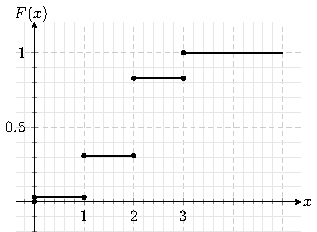
\includegraphics[width=0.5\linewidth]{mai_fig045.pdf}
      \caption{Distribuční funkce k příkladu \ref{mai:exam064}. \cite[s.~233]{Musilova2009MA1}}
      \label{mai:fig045}
    \end{figure}
    Zadáním distribuční funkce je naopak jednoznačně určeno rozdělení veličiny \(X\). Pro jednotlivé
    pravděpodobnosti totiž platí
    \begin{equation*}
      p_j = F(x_j) - F(x_{j-1})\qquad\text{pro}\qquad 2\leq j \leq k, \qquad p_1 = F(x_1).
    \end{equation*}
    
    Hledejme nyní hodnotu \(\overline{x}_P\) definovanou tak, že pravděpodobnost, že při náhodném 
    opakování pokusu nabude veličina \(X\) kterékoli z přípustných hodnot \(x_j \leq 
    \overline{x}_p\), je rovna \(P\). Znamená to, že pro \(x = \overline{x}_P\) má distribuční 
    funkce nabýt předepsané hodnoty \(P\). Abychom \(\overline{x}_P\), takzvaný 
    \(P\)\textbf{-kvantil}, určili, řešíme rovnici
    \begin{equation}\label{mai:eq064}
      \sum_{j=1}^{s}p_j = P
    \end{equation}
    vzhledem k neznámému počtu sčítanců \(s\). V případě veličiny s diskrétním rozdělením se ovšem
    může stát, že pro nevhodně zvolenou hodnotu \(P\) nebude mít rovnice řešení. To proto, že 
    veličina \(X\) může nabývat jen hodnot, které lze očíslovat přirozenými čísly, takže při každé 
    změně horní meze sumy \(s\) o jedničku se suma mění skokem. Vidíme to jak v předcházející 
    tabulce, tak v grafu na obrázku \ref{mai:fig045}. Pro \(P = \num{0.5}\) se \(P\)-kvantil 
    \(\overline{x}_p\), pokud je vůbec definován, nazývá \textbf{medián}. Značí se pouze 
    \(\overline{x}\).

    %--Ještě střelba------------------------------------------------
    % !TeX spellcheck = cs_CZ
\begin{mdframed}[style=mdexam]
  \begin{example}\label{mai:exam067}
    \textbf{Ještě střelba}\newline
    Problém s definici \(P\)-kvantilu u veličiny s diskrétním rozdělením snadno vidíme na příkladu
    střelby (příklad \ref{mai:exam064}). Pro \(s\) postupně 1, 2, 3, 4 nabývá součet na levé straně
    rovnice (\ref{mai:eq064}) hodnot
    
    \begin{equation*}
      p_1 = \num{0.003},\; p_1 + p_2 = \num{0.31},\; p_1 + p_2 + p_3 = \num{0.83}, 
    \end{equation*}
    \begin{equation*}
      p_1 + p_2 + p_3 + p_4 = 1.
    \end{equation*}
    Pojem \(P\)-kvantil je tedy definován jen pro \(P = 0\), \(P = \num{0.03}\), \(P = \num{0.31}\),
    \(P = \num{0.83}\) a \(P = 1\). (Pro \(P = 0\) a \(P = 1\) nemá žádný praktický význam.)
    Nenabývá-li \(P\) žádné z přípustných hodnot, tj. některé hodnoty z množiny \(\{\num{0.03},
    \num{0.31}, \num{0.83}, 1\}\), nemá rovnice pro s řešení a \(P\)-kvantil není vůbec definován.
    Je-li hodnotou \(P\) některý prvek této množiny, dostaneme z rovnice (\ref{mai:eq064}) sice
    jediné řešení \(s\), avšak která hodnota bude \(P\)-kvantilem? Z grafu je vidět, že pro každou
    přípustnou hodnotu \(P\) vyhovuje podmínce celý interval proměnné \(x\). Konkrétní výsledky
    shrnuje následující tabulka:
    
    {\centering
      \begin{tabular}{c|@{\hspace{3pt}}c@{\hspace{3pt}}c@{\hspace{3pt}}c@{\hspace{3pt}}c@{\hspace{3pt}}c}
        \(P\) & \num{0} & \num{0.03} & \num{0.31} & \num{0.83} & \num{1} \\ \hline
        \(F(x) = P\) & \((-\infty,\num{0})\) & \(\left[0, 1\right)\) &
        \(\left[1, 2\right)\) & \(\left[2, 3\right)\) & \(\left[3, \infty\right)\)
      \end{tabular}
    \par}
    
    Význam pojmu \(P\)-kvantil je tedy pro náhodnou veličinu s diskrétním rozdělením poněkud sporný.
    Uplatní se však velmi dobře u veličin s rozdělením spojitým, jak uvidíme později. Než však
    opustíme příklad se střelbou definitivně, spočtěme si ještě střední hodnotu a rozptyl veličiny
    \(X\), kterou jsme definovali jako počet dosažených bodů při jednom výstřelu:
    \begin{align*}
      \langle x \rangle 
          &= \sum_{j=1}^{4}x_jp_j                                                                \\
          &= 0\cdot\num{0.03} + 1\cdot\num{0.28}+ 2\cdot\num{0.52} + 3\cdot\num{0.17} = \num{1.83}, 
    \end{align*}
    \begin{align*}
      D(X)  &= \sum_{j=1}^{4}\left(x_j - \langle x \rangle \right)^2p_j                          \\
            &= (0-\num{1.83})^2\cdot\num{0.03}+(1-\num{1.83})^2\cdot\num{0.28}                   \\
            &+ (2-\num{1.83})^2\cdot\num{0.52}+(3-\num{1.83})^2\cdot\num{0.17}                   \\
                &\simeq\num{0.541},                                                              \\
      \sigma(x) &\simeq\num{0.736}.
    \end{align*}

    V příkladu \ref{mai:exam064} jsme odhadovali, kolika bodů dosáhne střelec při pěti výstřelech.
    Tato hodnota nám vyšla \(\num{5}\cdot\num{1.83} = \num{9.15} = 9\). Nyní vidíme je jí souvislost
    se střední hodnotou náhodné veličiny \(X\). Pokud totiž definujeme veličinu \(Y\) jako počet
    bodů dosažených při pěti výstřelech, je \(Y = 5X\) a \(\langle y \rangle = 5\langle x \rangle\).
    Uvažujme nyní o významu směrodatné odchylky. Zřejmě \(\sigma(y) = 5\sigma(x) = \num{3.68}\).
    Směrodatná odchylka \(\sigma(y)\) určuje interval \((\langle y \rangle - \sigma(y), \langle y
    \rangle + \sigma(y)) = (\num{5.32}, \num{12.68})\). Možnosti bodového zisku ležící v tomto
    intervalu jsou \num{6} až \num{12} bodů včetně. Pokud bychom doplnili tabulku z příkladu
    \ref{mai:exam064} ještě o rozklady a jejich pravděpodobnosti pro bodový součet při pěti
    výstřelech \(j = \num{6}\) a \(j = \num{12}\), dostaneme \(p(A_6) = \num{0.0400}\), \(p(A_{12})
    = \num{0.0550}\). Pravděpodobnost, že výsledek střelce leží při pěti výstřelech v intervalu
    \((\langle y \rangle - \sigma(y), \langle y \rangle + \sigma(y)) = (\num{5.32}, \num{12.68})\),
    je tedy
    \begin{align*}
      \sum_{j=6}^{12}p(A_j) &= p(A_6) + \sum_{j=7}^{11}p(A_j) + p(A_{12})                \\
                            &= \num{0.0400} + \num{0.873} + \num{0.0550} \simeq \num{0.97}.
    \end{align*}
    Při výpočtu jsme využili výsledku z příkladu \ref{mai:exam064}, kde jsme počítali
    pravděpodobnost, že střelec dosáhne bodového výsledku v rozmezí \num{7} až \num{11} bodů.
    Směrodatná odchylka \(\sigma(y)\) veličiny \(Y\) určuje tedy v tomto případě interval okolo
    střední hodnoty \(\langle y \rangle\), v němž leží střelcův bodový zisk s velmi vysokou
    pravděpodobností \SI{97}{\percent}. Tento výsledek lze velmi názorně interpretovat také takto:
    Vystřelí-li střelec pětkrát na terč, bude téměř s jistotou jeho bodový zisk ležet v intervalu
    určeném směrodatnou odchylkou, tj. bude ležet mezi šesti a dvanácti body. Není vyloučeno, že
    bodový zisk bude třeba pět bodů, nebo i nula, nebo naopak dokonce maximálních možných patnáct
    bodů. Všechny ty to možnosti dohromady jsou však vysoce nepravděpodobné, připadá na ně
    pravděpodobnost pouhé \SI{3}{\percent}!. Anebo ještě trochu jinak: Kdyby střelec při tréninku
    uskutečnil třeba sto sérií po pěti výstřelech, pak by skoro jistě bylo sedmadevadesát z nich v
    rozmezí bodového zisku \num{6} až \num{12} bodů a tři mimo. Toto konstatování ovšem opět
    nevylučuje možnost, že v rozmezí \num{6} až \num{12} bodů bude ležet jiný počet sérií než
    \num{97}. Může dokonce v principu dojít k tomu, že do této kategorie padnou série všechny nebo
    žádná. Takový výsledek je však opět vysoce nepravděpodobný.
    
    Není vyloučeno, že i po prostudování tohoto příkladu bude někdo stále nespokojen s tím, že je
    naše vyjadřování „málo přesné“. Vzhledem k pravděpodobnostnímu charakteru posuzovaných jevů
    však, bohužel, přesnější být nemůže.
  \end{example}
\end{mdframed}
    %---------------------------------------------------------------
    
    Příklad \ref{mai:exam067} názorně vypovídá o významu směrodatné odchylky. Viděli jsme, že 
    intervalu o šířce \(2\sigma(y)\) s hodnotou \(\langle y \rangle\) uprostřed odpovídá vysoká 
    pravděpodobnost, že v něm bude ležet bodový zisk střelce při každé pětici výstřelů. Čím bude 
    tento interval užší, tím v průměru blíže budou jednotlivé hodnoty bodového zisku ležet v 
    blízkosti střední hodnoty. Mohli bychom říci, že střelec, jehož výsledky vykazují malou 
    směrodatnou odchylku resp. malý rozptyl, míří přesněji. Směrodatná odchylka je tedy v jistém 
    smyslu jedním z parametrů charakterizujících kvalitu střelby - střelba s malou hodnotou  
    \(\sigma(y)\) je přesnější než střelba s velkou hodnotou \(\sigma(y)\). Druhým parametrem 
    kvality střelby, který je pro její hodnocení z hlediska možnosti vyhrávat soutěže jistě 
    podstatně důležitější, je samozřejmě samotná střední hodnota bodového zisku. Čím je větší, tím 
    je střelcovo pořadí při závodech lepší. Pro interpretaci směrodatné odchylky to ovšem není 
    podstatné. Kdybychom porovnávali dva střelce, jejichž střední bodový zisk při
    pěti výstřelech je třeba \num{12} bodů a \num{3} body, avšak směrodatná odchylka je u obou 
    stejná, musíme konstatovat, že oba jsou stejně přesní. Jeden z nich však systematicky dělá 
    nějakou chybu a přesně střílí do nesprávného místa. Význam pojmu přesnost z hlediska hodnocení 
    náhodných veličin je tedy oproti jeho běžnému chápání poněkud posunut.
    
    Všimněme si ještě jedné důležité obecné věci: Tvar vzorce pro výpočet rozptylu resp. směrodatné 
    odchylky je stejný pro všechny typy rozdělení. Konkrétní pravděpodobnost, že hodnota
    veličiny padne do intervalu určeného směrodatnou odchylkou, tj. do intervalu \((\langle y 
    \rangle - \sigma(y), \langle y \rangle + \sigma(y))\), však pochopitelně na konkrétním 
    rozdělení závisí.

    %--Poissonovo rozdělení-----------------------------------------
    % !TeX spellcheck = cs_CZ
\wikitextrule
\begin{example}\label{mai:exam068}
  \textbf{Poissonovo rozdělení}\newline\small
  Limitním případem Bernoulliova (binomického) rozdělení pro velké hodnoty \(n\), tj. \(n 
  \rightarrow \infty\), a pro \(j \ll n\) je \textbf{rozdělení Poissonovo}. Odvodíme je. Pro velká 
  \(n\) a \(j \ll n\) platí přibližný vzorec
  \begin{equation*}
    n! \simeq n^j(n-j)!,
  \end{equation*}
  a tedy
  \begin{equation*}
    P_j \simeq \lim\limits_{n\rightarrow\infty}\dfrac{n^j}{j!}p^j(1-p)^{n - j}
        \simeq \lim\limits_{n\rightarrow\infty}\dfrac{(np)^j}{j!}\left(1-\dfrac{np}{n}\right)^{n}.
  \end{equation*}
  Při vzpomínce na kapitolu o počítání i limitami a na \textbf{l’Hospitalovo pravidlo} snadno 
  provedeme následující výpočet. O testujte své předchozí znalosti a jednotlivé kroky výpočtu 
  proveďte:
  \begin{equation*}
    \lim\limits_{n\rightarrow\infty}\left(1 - \dfrac{A}{n}\right)^n = 
    \lim\limits_{x\rightarrow0}\left(1 - Ax\right)^\dfrac{1}{x} =
    \exp\left(\lim\limits_{x\rightarrow0}\dfrac{\ln(1 - Ax)}{x}\right) = e^{-A}.
  \end{equation*}
  V našem případě je \(A = np = \langle x \rangle\) (střední hodnota veličiny \(X\) při 
  Bernoulliově rozdělení), takže
  \begin{equation}\label{mai:eq065}
    p_j = \langle x \rangle^j\dfrac{e^{-\langle x \rangle}}{j!}.
  \end{equation}
  Možnost použití Bernoulliova rozdělení si již představit dokážeme. Přinejmenším jsou hody mincemi 
  a kostkami pěkné hříčky. K čemu však je dobré rozdělení Poissonovo? Ja k může vypadat praktická 
  situace, kdy provádíme obrovské množství opakování pokusu a zajímá nás pravděpodobnost pouze 
  malého počtu zdarů? Typickým příkladem takové situace je registrace částic vznikajících při 
  radioaktivním rozpadu. Taková měření jsou potřebná nejen ve fyzikálním výzkumu, ale i v 
  aplikovaných oborech, například v lékařství. Počet \(n\) radioaktivních rozpadů za jednotku času, 
  například za sekundu, je u běžných zdrojů obrovský, zatímco počet těch z nich, které jsou 
  zachycovány detektorem, může být při určitých experimentech malý. Částice se registrují
  pomocí Geigerova-Mullerova počítače, kterým je ionizační komora pracující ve vhodném režimu. 
  Pokud je počet částic \(j\) dopadajících za jednu sekundu do detektoru velmi malý, vyvolá každá z 
  nich měřitelný a dokonce slyšitelný pulz (v obvodu to „praská“). Po registraci částice potřebuje 
  detektor jistou \textbf{mrtvou dobu}, aby se vrátil do výchozího stavu, v němž je schopen 
  registrovat další částici. Tato doba se pohybuje kolem \SI{e-4}{s}. Aby byly jednotlivé pulzy 
  dobře odlišeny, je však třeba, aby do detektoru dopadlo za jednu sekundu mnohem a mnohem méně 
  částic, než jak by odpovídalo převrácené hodnotě mrtvé doby. Zejména pokud bychom chtěli pulzy 
  počítat sluchem, nemělo by jich být více než zhruba jeden až dva každou sekundu. Uvažujme o 
  radioaktivním rozpadu jader cesia \ce{Cs^137}. Jedná se o takzvaný \textbf{beta-rozpad}, který 
  probíhá následovně:
  \begin{itemize}
    \item \ce{Cs^137} \(\longrightarrow\) \ce{Ba^137} + elektron + neutrino, asi \SI{8}{\percent} 
          všech rozpadů
    \item \ce{Cs^137} \(\longrightarrow\) \ce{Ba^137}* + elektron + neutrino, asi \SI{92}{\percent} 
          všech rozpadů
  \end{itemize}
  Excitované baryum \ce{Ba^137}* (jádro má vyšší energii než atom \ce{Ba^137} v základním stavu 
  asi o \SI{0.66}{\mega\electronvolt}  - odpovídá energii \SI{1.1e-13}{\joule}) se pak dále rozpadá 
  podle vzorce
  \begin{itemize}
    \item \ce{Ba137}* \(\longrightarrow\) \ce{Ba137} + částice gama.
  \end{itemize}

  Ze všech částic, které při reakci vznikají, se v Geigerově-Můllerově detektoru registrují 
  elektrony a částice gama, nelze je však od sebe odlišit. Uvažujme o cesiovém zdroji s běžnou 
  hodnotou aktivity, například \SI{10}{\pico\coulomb} (mikrocurie). Jednotka aktivity 
  radioaktivních preparátů \num{1} curie představuje situaci, kdy se za jednu sekundu rozpadá 
  \num{3.7e10} jader. Počet rozpadů, které v průměru nastanou třeba za deset sekund v našem vzorku, 
  je \(n = \num{3700000}\). V Bernoulliově pokusu to odpovídá počtu jeho opakování \(n\). Ja k jsme 
  již řekli, je to obrovský počet. Nastavíme-li experiment tak, abychom registrovali každou sekundu 
  zhruba jednu částici (uslyšíme jeden „prásk“ ), bude počet zdarů \(j\) v Bernoulliově pokusu 
  velmi malý ve srovnání s \(n\). Jsou tedy splněny podmínky pro použití Poissonova rozdělení. 
  Zvolíme například desetisekundový interval měření a počítáme pulzy. Počet registrovaných pulzů 
  \(j\) v tomto intervalu je roven počtu zdarů. Takové měření provedeme třeba dvěstěkrát.
  Označme počet intervalů, v nichž jsme naměřili právě \(j\) pulzů, jako \(\nu(j)\). Celkem je v 
  \(\nu(1) + \cdots + \nu(j_{max}) = \num{200}\). Získáme tak tabulku nebo graf, z nichž pak lze 
  usuzovat na parametry Poissonova rozdělení:
  \begin{table}[ht!]
    \centering
    \resizebox{0.8\textwidth}{!}{%
    \begin{tabular}{c|crrrrrrrrrrrrrrrrr}
      \(j\)      & 0 & 1 & 2 & 3 & 4 & 5 & 6 & 7 & 8 & 9 & 10 & 11& 12& 13 & 14 & 15 & 16 & 17   \\
      \hline
      \(\nu(j)\) & 0 & 4 & 10 & 19 & 28 & 33 & 34 & 26 & 19 & 10 & 6 & 3 & 2 & 2 & 2 & 0 & 1 & 1 \\
    \end{tabular}}
    % \caption{ }
  \end{table}
  Budeme-li předpokládat, že větší počet pulzů v desetisekundovém intervalu je již velmi málo 
  pravděpodobný, můžeme četnosti \(\nu(j)\) považovat za úměrné pravděpodobnostem \(p_j\) 
  Poissonova rozdělení. Všimněme si formule pro Poissonovo rozdělení podrobněji. Je vidět, že platí
  \begin{equation*}
    \dfrac{\nu(j + 1)}{\nu(j)} = \dfrac{p_{j+1}}{p{j}} = \dfrac{\langle x \rangle}{j + 1},
    \qquad p_0 = e^{-\langle x \rangle}.
  \end{equation*}
  Pro hodnotu \(j\), pro kterou jsou si četnosti \(\nu(j)\) a \(\nu(j + 1)\) „nejblíže“, je 
  \(\langle x \rangle \simeq j + 1\). Z tabulky vidíme, že v případě našeho experimentu je 
  \(\langle x \rangle = 6\). Hodnota \(p_0 = e^{-6} \simeq \num{0.002}\) je tedy tak malá, že se 
  ani nedivíme, že jsme mezi dvěma stovkami měření nezaznamenali ani jeden případ, kdy v 
  desetisekundovém intervalu nebyla zaregistrována žádná částice.
  
  Můžeme ještě určit podíly sousedních hodnot \(\nu(j + 1)\) a \(\nu(j)\) a zjistit, zda výsledky 
  našeho experimentu odpovídají vlastnostem Poissonova rozdělení:
  \begin{table}[ht!]
    \centering
    \resizebox{0.7\textwidth}{!}{%
    \begin{tabular}{c|crrrrrrrr}
      \(j\)               & 0 & 1 & 2  & 3  & 4  & 5  & 6  & 7 & 8    \\ \hline
      \(\nu(j+1)/\nu(j)\) & - & \num{2.50} & \num{1.90} & \num{1.47} & \num{1.18} 
                          & \num{1.03} & \num{0.76} & \num{0.73} & \num{0.53}   \\
      \(\langle x \rangle / j + 1\) & \num{6.00} & \num{3.00} & \num{2.00} & \num{1.50} & \num{1.20}
                          & \num{1.00} & \num{0.86} & \num{0.75} & \num{0.67}
    \end{tabular}}
    % \caption{ }
  \end{table}
  \begin{table}[ht!]
    \centering
    \resizebox{0.7\textwidth}{!}{%
    \begin{tabular}{c|crrrrrrrr}
      \(j\)               & 9 & 10 & 11  & 12  & 13  & 14  & 15  & 16 & 17    \\ \hline
      \(\nu(j+1)/\nu(j)\) & \num{0.60} & \num{0.50} & \num{0.67} & - & - & - & - & - & -   \\
      \(\langle x \rangle / j + 1\) & \num{0.60} & \num{0.55} & \num{0.50} & \num{0.46}
                          & \num{0.43} & \num{0.40} & \num{0.38} & \num{0.35} & \num{0.33}
    \end{tabular}}
    % \caption{ }
  \end{table}
  Vidíme, že hodnoty podílů sousedních četností celkem dobře odpovídají vlastnostem Poissonova 
  rozdělení pro \(0 \leq j \leq 12\). Pro \(j > 12\) jsou již četnosti \(\nu(j)\) tak malé, že 
  vytvářet jejich podíly nemá smysl. Tato skutečnost je v tabulce vyznačena pomlčkou.
  
  Poissonovým rozdělením se řídí také například četnost červených krvinek, které se v daném časovém 
  intervalu objeví ve vymezené části zorného pole mikroskopu, četnost zmetků v dodávce zboží, 
  četnost překlepů písařky, apod.  
\normalsize
\end{example}
    %---------------------------------------------------------------
    
    \subsection{Kolik rychlostí má molekula plynu - spojité rozdělení}
      Již nadpis napovídá, že veličina se spojitým rozdělením může zřejmě nabývat „spojitě 
      rozložených“ hodnot, tj. přípustným i hodnotami budou například právě všechna čísla \(x\) z 
      jistého intervalu, \(x\in[a, b]\). Jaká však bude pravděpodobnost \(p(x)\), že veličina \(X\) 
      nabývá právě hodnoty \(x\in[a, b]\)? Jestliže víme, že „součet“ všech \(p(x)\) musí být roven 
      jedné, vzniká problém.
      
      Hodnot \(x\) je totiž nekonečně (dokonce nespočetně) mnoho! Je jich tolik, jako je čísel na 
      celé reálné ose. A kdyby byla pravděpodobnost \(p(x)\) jakkoli malinkatá, nikdy nebude součet 
      všech \(p(x)\) konečný. Pravděpodobnost nabývání hodnoty \(x\) tedy musí být nulová. Vzniklou 
      překážku odstraníme snadno. Rozdělení náhodné veličiny \(X\) bude nutno charakterizovat 
      nikoli pravděpodobností, ale \textbf{hustotou pravděpodobnosti}. Je to obdobná situace jako 
      třeba při popisu rozložení hmotnosti nějakého tělesa, předpokládáme-li, že je ta to hmotnost 
      rozložena v objemu tělesa spojitě. Také nemá příliš smysl se ptát, jaká je hmotnost jednoho 
      bodu tohoto tělesa. I zde by byla odpověď, že nulová. Spíše si vždy klademe otázku, jaká je 
      hmotnost \(\Delta m(\vec{r})\) jistého malého objemu \(\Delta V\), například malého kvádříku, 
      umístěného třeba jedním z vrcholů v bodě o poloze \(\vec{r}\). Hustota \(\varrho(\vec{r})\) 
      tělesa v bodě \(\vec{r}\) je pak limitou podílu \(\Delta m(\vec{r})/\Delta V\) pro \(\Delta V 
      \longrightarrow 0\). Obdobně je tomu i s rozdělením spojité náhodné veličiny \(X\). 
      Zvolíme-li pro jistou hodnotu \(x\) interval \([a, x + \Delta x]\), má smysl otázka, jaké je 
      pravděpodobnost \(\Delta p(x)\), že veličina nabývá hodnoty (kterékoli) právě z tohoto 
      intervalu.

      \adjustbox{minipage=[c]{\textwidth}}{%
        Limitu
        \begin{equation}\label{mai:eq066}
          w(x) = \lim\limits_{\Delta\longrightarrow0}\dfrac{\Delta p(x)}{\Delta x}
        \end{equation}
        nazýváme \textbf{hustotou pravděpodobnosti} veličiny \(X\) v bodě \(x\) (pro \(x = a\), 
        resp. \(x = b\) se jedná o limitu zprava, resp. zleva).
      }
      
      Přímo tato funkce pak představuje ono spojité rozdělení náhodné veličiny \(X\). Určuje totiž
      hustotu pravděpodobnosti \(w\) pro hodnotu \(x\) náhodné veličiny \(X\), obdobně jako \(p_j\) 
      v případě diskrétního rozdělení určuje pravděpodobnost hodnoty \(x_j\). Předpokládejme, že je 
      funkce \(w(x)\) na intervalu \([a, b]\) spojitá.
  
      \adjustbox{minipage=[c]{\textwidth}}{%
        Pro \(x \in [a, b]\) definuje integrál jako funkce horní meze
        \begin{equation}\label{mai:eq067}
          F(x) = \int_a^xw(u)\dd{u}
        \end{equation}
        \textbf{distribuční funkci}.
      }
      Jeho hodnota pro dané \(x\) udává pravděpodobnost, že hodnota veličiny \(X\) padne do 
      intervalu \([a, x]\), opět v plné analogii s případem diskrétního rozdělení. Na \((a, b)\) je 
      tedy hustota pravděpodobnosti \(w(x)\) derivací distribuční funkce. Je zřejmé, že \(F(b) = 
      1\). Integrál z hustoty pravděpodobnosti v mezích \([a, b]\) udává totiž pravděpodobnost, že 
      hodnota veličiny \(X\) padne do intervalu přípustných hodnot, tedy pravděpodobnost jistého 
      jevu. V případě diskrétního rozdělení jsme však distribuční funkci definovali nejen pro 
      přípustné hodnoty náhodné veličiny, ale pro všechna x \in (-\infty, +\infty). Tento postup 
      budeme respektovat i nyní a definujeme
      \begin{equation*}
        F(x) = 0\text{ pro }x \in (-\infty,a)\text{ a }F(x) = 1\text{ pro }x \in (b , +\infty).
      \end{equation*}
      \adjustbox{minipage=[c]{\textwidth}}{%
        \begin{equation}\label{mai:eq068}
          \langle x \rangle = \int_a^bxw(x)\dd{x}, \qquad 
                       D(X) = \int_{a}^{b}(x - \langle x \rangle)^2w(x)\dd{x}.
        \end{equation}
      }
      \textbf{Relativní směrodatná odchylka} je opět podílem \(\sqrt{D(X)}/\langle x \rangle\), 
      nejpravděpodobnější hodnota neboli \textbf{modus} \(x_m\) je taková hodnota veličiny \(X\) , 
      pro kterou je hustota pravděpodobnosti maximální
      
      Daleko lépe než u veličin s diskrétním rozdělením vypadá možnost definovat \(P\)-kvantil 
      \(\tilde{x}_p\) a \textbf{medián} \(\tilde{x}\). Jsou jednoduše řešením rovnic
      \begin{equation*}
        F(\tilde{x}_P) = P, \qquad F(\tilde{x}) = \dfrac{1}{2}
      \end{equation*}
      (Mohli bychom mediánu třeba i říkat „půlkvantil“. To ale není zvykem.) \(P\)-kvantil je 
      definován pro jakoukoli hodnotu \(P\) zadanou v intervalu \((0, 1)\). Skutečně, hustota 
      pravděpodobnosti je nezápornou funkcí na intervalu \([a, b]\) (podle předpokladu i spojitou), 
      takže distribuční funkce je na \([a, b]\) \emph{spojitá} a \emph{rostoucí} a nabývá hodnot 
      \(0 = F(a) \leq F(x) \leq F(b) = 1\). Podle jedné z vět o spojitých funkcích (odstavec 
      2.1.7*) nabývá funkce spojitá na uzavřeném intervalu všech hodnot mezi svým minimem a 
      maximem. V intervalu \([a, b]\) tedy existuje alespoň jedna hodnota \(\tilde{x}_P\) , pro 
      kterou je \(F(\tilde{x}_P) = P\). Ze skutečnosti, že je \(F(x)\) navíc rostoucí, vyplývá, že 
      i \(\tilde{x}_P\) existuje jednoznačně.
  
      Tyto závěry zůstanou v platnosti, i kdyby veličina \(X\) nabývala svých hodnot v intervalu
      typu \(\left[0, \infty\right), \left(—\infty, b\right]\) nebo \((—\infty, \infty)\). Vzhledem 
      k požadavku
      \begin{equation*}
        \int_{a}^{b}w(x)\dd{x} = 1,
      \end{equation*}
      kde kterákoli z mezí \(a\), resp. \(b\) může být i nevlastní, je zřejmé, že funkce \(w(x)\) 
      musí být na svém definičním oboru \(D_f\) omezená. Navíc je na něm spojitá. Vybereme-li tedy 
      jakýkoli uzavřený podinterval oboru \(D_f\), můžeme předchozí argumentaci týkající se 
      \(P\)-kvantilu bez problémů použít.

      %--Normální rozdělení-------------------------------------------
      % !TeX spellcheck = cs_CZ
\begin{mdframed}[style=mdexam]
\begin{example}\label{mai:exam069} \textbf{Normální rozdělení}\\
  Veličinou s normálním rozdělením rozumíme takovou náhodnou veličinu \(X\), jejíž hustota 
  pravděpodobnosti má tvar
  \begin{mdframed}[style=highlight]
    \begin{equation}\label{mai:eq069}
      w(x) = \dfrac{1}{\sigma\sqrt{2\pi}}\exp\left[-\dfrac{(x-\mu)^2}{2\sigma^2}\right],
             \qquad x\in(-\infty, \infty).
    \end{equation}
  \end{mdframed}
  Grafem této funkce je \textbf{Gaussova křivka}. Distribuční funkce má tvar
  \begin{mdframed}[style=highlight]
    \begin{equation}\label{mai:eq70}
      F(x) = \int_{-\infty}^{x}\dfrac{1}{\sigma\sqrt{2\pi}}
               \exp\left[-\dfrac{(t-\mu)^2}{2\sigma^2}\right]\dd{t}.
    \end{equation}
  \end{mdframed}
  udává pravděpodobnost, že hodnota náhodné proměnné je menší než zadaná hodnota (nerovnost může 
  být i neostrá). Přitom \(F(\infty) = 1\) (pravděpodobnost jistého jevu). Skutečně, platí
  \begin{equation*}
    \begin{multlined}
      \int_{-\infty}^{\infty}\dfrac{1}{\sigma\sqrt{2\pi}}
      \exp\left[-\dfrac{(t-\mu)^2}{2\sigma^2}\right]\dd{t}   \\
      \shoveleft[1cm]= \dfrac{\sigma\sqrt{2}}{\sigma\sqrt{2\pi}}
              \int_{-\infty}^{\infty}\exp\left(-u^2\right)\dd{u} =1.
    \end{multlined}
  \end{equation*}
  Takzvaný Laplaceův integrál \(\int_{-\infty}^{\infty}\exp(-u^2)\dd{u} = \sqrt{\pi}\) 
  sice můžeme najít v tabulkách a v dalším dílu jej i odvodíme, v tu to chvíli se však budeme řídit 
  výrokem lorda Kelvina: „Matematik je ten, komu je toto zřejmé jako je zřejmé vám, že dvakrát dvě 
  jsou čtyři.“ Příklady normálního rozdělení pro různé hodnoty \(\sigma,\,\mu\) a odpovídající 
  distribuční funkce vidíme na obrázku \ref{mai:fig046a} a \ref{mai:fig046b}.

  {\centering
    \captionsetup{type=figure}
     \subcaptionbox{\label{mai:fig046a}}{\luafigure[1]{mai_fig046a.pdf}}              \\
     \subcaptionbox{\label{mai:fig046b}}{\luafigure[1]{mai_fig046b.pdf}}
     \captionof{figure}{Hustota pravděpodobnosti normálních rozdělení a jejich distribuční funkce 
              s různými charakteristikami \(\sigma\) a \(\mu\). Červenou čárou je vyznačeno 
              normované normální rozdělení. \cite[s.~240]{Musilova2009MA1}
    \label{mai:fig046}}
  \par}
  \vspace*{10px} Určíme střední hodnotu a rozptyl veličin s tímto rozdělením:
  \begin{align*}
    \langle x \rangle 
      &= \int_{-\infty}^{x}\dfrac{1}{\sigma\sqrt{2\pi}}x\cdot
         \exp\left[-\dfrac{(x-\mu)^2}{2\sigma^2}\right]\dd{x}                                     \\
      &= \dfrac{\sigma\sqrt{2}}{\sigma\sqrt{2\pi}}
         \int_{-\infty}^{\infty}\left(\mu+t\sigma\sqrt{2}\right)\cdot\exp\left(-t^2\right)\dd{t}  \\
      &= \dfrac{\mu}{\sqrt{\pi}}\int_{-\infty}^{\infty}\exp\left(-t^2\right)\dd{t}                \\
      &+ \dfrac{1}{\sqrt{\pi}}\int_{-\infty}^{\infty}t\sigma\sqrt{2}\cdot\exp\left(-t^2\right)\dd{t}
       =\mu.
  \end{align*}
  Druhý z integrálů je totiž roven nule, neboť integrand je lichá funkce.
  \begin{align*}
    D(X)  &= \dfrac{1}{\sigma\sqrt{2\pi}}\int_{-\infty}^{\infty}\left(x - \mu\right)^2 
             \exp\left[-\dfrac{(x-\mu)^2}{2\sigma^2}\right]\dd{x}                                \\
          &= \dfrac{2\sqrt{2}\sigma^3}{\sigma\sqrt{2\pi}}
             \int_{-\infty}^{\infty}t^2\exp\left(-t^2\right)\dd{t}
           = \sigma^2.
  \end{align*}
  Integrál \(\int_{-\infty}^{\infty}t^2\exp\left(-t^2\right)\dd{t} = \frac{\sqrt{\pi}}{2}\) lze buď 
  opět najít v tabulkách, nebo jej metodou per partes převést na výpočet Laplaceova integrálu:
  \begin{align*}
    I &= \int_{-\infty}^{\infty}t\cdot t\exp\left(-t^2\right)\dd{t}         \\
      &= \left[-\dfrac{t}{2}\exp\left(-t^2\right)\right]_{-\infty}^{\infty}
       + \dfrac{1}{2}\int_{-\infty}^{\infty}\exp\left(-t^2\right)\dd{t}.
  \end{align*}
  
  Distribuční funkce normálního rozdělení, zvaná \(errorfunkce\), je běžnou součástí různých 
  počítačových programů, takže poměrně snadno zjistíme pravděpodobnostní obsah intervalu určeného 
  směrodatnou odchylkou \(\sigma(x) = \sqrt{d(X)} = \sigma\). Pravděpodobnost, že hodnota náhodné 
  veličiny \(X\) s normálním rozdělením leží v intervalu \((\mu - \sigma, \mu + \sigma)\), je 
  zhruba \SI{68.3}{\percent}. V souvislosti s normálním rozdělením se často užívají další 
  dva druhy odchylek. \textbf{Pravděpodobná chyba} \(\theta\) určuje interval \((\mu - \theta, \mu 
  + \theta)\), v  němž leží hodnota veličiny \(X\) s pravděpodobností \SI{50}{\percent}. 
  \textbf{Krajní chyba} \(\kappa\) určuje interval \((\mu - \kappa, \mu + \kappa)\), v němž leží 
  hodnota veličiny \(X\) s pravděpodobností \SI{99.7}{\percent}. Z tabelovaných hodnot 
  \(errorfunkce\) zjistíme, že platí
  \begin{equation}\label{mai:eq71}
   \theta \simeq \dfrac{2}{3}\sigma, \qquad \kappa = 3\sigma
  \end{equation}
  Poznamenejme, že normálním rozdělením \(w(x)\) (\ref{mai:eq069}) lze přibližně nahradit 
  Bernoulliovo rozdělení
  \begin{align*}
    w_{Ber}(x)        &= \binom{n}{x}p^x(1 - p)^{n-x},  \\
    \langle x \rangle &= np, \;  D(x) = np(1-p)
  \end{align*}
  pro velké hodnoty \(n\) a také Poissonovo rozdělení
  \begin{equation*}
    w_{Pois}(x) = e^{-\langle x \rangle}\dfrac{\langle x \rangle^x}{x!}, \qquad 
    D(x) = \langle x \rangle
  \end{equation*}
  s velkou střední hodnotou \(\langle x \rangle\)
\end{example}
\end{mdframed}
      %---------------------------------------------------------------
  
      %--Kolik rychlostí má molekula plynu----------------------------
      % !TeX spellcheck = cs_CZ
\wikitextrule
\begin{example}\label{mai:exam070}
  \textbf{Kolik rychlostí má molekula plynu}\newline\small
  Tato otázka se zdá na první pohled zcela nesmyslná. Každý student fyziky ví, že molekuly plynu 
  lze popisovat jako klasické částice, jejichž mechanický stav je jednoznačně určen polohovým 
  vektorem a vektorem rychlosti. Molekula má tedy vždy určitou hodnotu rychlosti. Představte si ale 
  takový plyn ve skutečnosti. Jeden mol jeho látkového množství (např. pro kyslík to představuje 
  hmotnost \num{32} gramů) obsahuje asi \num{6.623e23} molekul! Kdybychom chtěli plyn popisovat 
  jako soustavu klasických částic v mechanice, museli bychom v daném okamžiku znát polohu a 
  rychlost každé molekuly z tohoto obrovského počtu. A to je principiálně nemožné, protože do 
  chování takové soustavy zasahuje velmi podstatným způsobem „náhoda“. Nemůžeme určit, ve kterém
  bodě prostoru právě daná molekula je a jak rychle se pohybuje. Dokážeme pouze určit, s jakou 
  pravděpodobností se nachází v elementárním objemu \(\Delta V = \Delta x \Delta y \Delta z\) v 
  okolí daného bodu o polohovém vektoru \(\vec{r}\) a s jakou pravděpodobností \(\Delta P\) leží 
  koncový bod vektoru její rychlosti v elementárním objemu \(\Delta\Omega = \Delta v_x \Delta v_y 
  \Delta v_z\) „rychlostního“ prostoru v okolí zadané rychlosti \(\vec{v}\). Uvažujme o 
  nejjednodušším modelu plynového tělesa, takzvaném ideálním plynu, jehož molekuly jsou stejné a 
  navzájem neinteragují s výjimkou kratičkých náhodných srážek. Molekuly takového plynu jsou z 
  hlediska pravděpodobnostního popisu navzájem ekvivalentní. Pravděpodobnost \(\Delta P\) bude pro 
  všechny stejná a pro velmi malé elementární objemy bude dána vztahem
  \begin{equation*}
    \Delta P(\vec{r},\vec{v}) = \varrho(\vec{r},\vec{v})\Delta V \Delta\Omega,
  \end{equation*}
  kde \(\varrho(\vec{r},\vec{v}) = \varrho(x, y, z, v_x, v_y, v_z)\) je odpovídající hustota 
  pravděpodobnosti. Jak ale hustota konkrétně závisí na polohách a rychlostech molekul? Tento 
  fyzikální zákon, zvaný \textbf{Gibbsovo rozdělení}, se řídí exponenciální funkcí
  \begin{equation*}
    \varrho(\vec{r},\vec{v}) = K\exp\left(-\dfrac{E(\vec{r},\vec{v})}{kT}\right)
  \end{equation*}
  kde \(E\) je \textbf{mechanická energie molekuly} (kinetická plus potenciální v případném silovém 
  poli), \(T\) je \textbf{absolutní teplota plynu} udávaná v kelvinech a \(k = 
  \SI{1.38e-23}{\joule\per\kelvin}\) je \textbf{Boltzmannova konstanta}.
  
  Zajímá-li vás, proč si příroda v tomto případě vybrala zrovna exponenciální funkci, sledujte 
  následující orientační úvahu: Rozdělme si v myšlenkách plynové těleso na dvě části, jimž 
  odpovídají energie \(E_1\) a \(E_2\). Celková energie soustavy je \(E = E_1 + E_2\). Označme 
  \(P(E)\) pravděpodobnost, že, se soustava nachází ve stavu s energií \(E\), pravděpodobnosti, že 
  se jednotlivé části nachází nezávisle ve stavech s energiemi \(E_1\) a \(E_2\), pak jako
  \(P(E_1)\) a \(P(E_2)\). Pravděpodobnost, že se první část soustavy nachází ve stavu s energií 
  \(E_1\) a \textbf{současně} druhá část ve stavu s energií \(E_2\), je rovna součinu 
  pravděpodobností těchto nezávislých jevů. Proto \(P(E_1 + E_2) = P(E_1) \cdot P(E_2)\). Tuto 
  vlastnost mají ovšem právě exponenciální funkce. Platí tedy \(\varrho \approx\exp(\beta E)\). 
  Konstantu \(\beta\) určí jen experiment, z něhož vychází \(\beta = - (kT)^{-1}\).
  
  Vrátíme se nyní k výchozímu problému, neboť úvodní otázka nabyla smyslu: Molekula může mít 
  libovolnou rychlost s větší či menší pravděpodobností. Nebude-li ideální plyn umístěn v žádném 
  silovém poli, bude mechanická energie molekuly dána pouze energií kinetickou. Elementární 
  pravděpodobnost, že koncový bod rychlosti molekuly leží v elementárním objemu \(\Delta\Omega\) v 
  okolí bodu \(\vec{v}\) „rychlostního“ prostoru, bez ohledu na to, v jaké části „obyčejného“, tj. 
  \textbf{konfiguračního prostoru} se vyskytuje, je
  \begin{equation*}
    \Delta P(\vec{v}) = \varrho(\vec{v})\Delta\Omega 
                      = C\exp\left(-\dfrac{m(v_x^2 + v_y^2 + v_z^2)}{2kT}\right)\Delta\Omega.
  \end{equation*}
  Tato pravděpodobnost, jak je vidět, nezávisí na směru rychlosti, pouze na její velikosti, 
  \(\varrho(\vec{v}) = \varrho(v)\). Konstantu \(C\) určíme snadno. Pravděpodobnost, že molekula má 
  vůbec nějakou rychlost, je rovna jedné (jistý jev). Matematický zápis této skutečnosti vyžaduje 
  znalost takzvaného trojného integrálu (integrujeme podle tří proměnných  - složek vektoru 
  rychlosti). V našem případě se však výpočet redukuje na součin tří integrálů jednoduchých,
  \begin{equation*}
    \int_{\Omega}\varrho(v_x, v_y, v_z)\dd{v_x}\dd{v_y}\dd{v_z} = 1
  \end{equation*}
  \begin{equation*}
    \Rightarrow C \cdot
     \int_{-\infty}^{\infty}\exp\left(\dfrac{mv_x^2}{2kT}\right)\dd{v_x} \cdot
     \int_{-\infty}^{\infty}\exp\left(\dfrac{mv_y^2}{2kT}\right)\dd{v_y} \cdot
     \int_{-\infty}^{\infty}\exp\left(\dfrac{mv_z^2}{2kT}\right)\dd{v_z} =1.
  \end{equation*}
  Po substitucích \(mv_i^2/2kT = u^2,\, i = x, y, z\) vede výpočet na \textbf{Laplaceův integrál}
  \begin{equation*}
    \int_{-\infty}^{\infty}\exp(-u^2)\dd{u} = \sqrt{\pi}.
  \end{equation*}
  Dostáváme
  \begin{equation*}
    C = \left(\dfrac{m}{2\pi kT}\right)^{\frac{3}{2}} \Rightarrow
    \Delta P(\vec{v}) = \left(\dfrac{m}{2\pi kT}\right)^{\frac{3}{2}}
                        \exp\left(- \dfrac{mv^2}{2 kT}\right)\dd{v_x}\dd{v_y}\dd{v_z}
  \end{equation*}
  Hustota pravděpodobnosti je stejná pro všechny koncové body vektoru rychlosti \(\vec{v}\) ležící 
  v rychlostním prostoru na kulové ploše o poloměru rovném velikosti rychlosti \(v\). Jaká bude 
  elementární pravděpodobnost \(\Delta P(v)\), že molekula má velikost rychlosti v intervalu \((v, 
  v + \Delta v)\) bez ohledu na směr pohybu? Tuto pravděpodobnost dostaneme, vezmeme-li za 
  \(\Delta\Omega\) objem tenké kulové slupky o poloměru \(v\) a tloušťce \(\Delta v\), v níž končí 
  všechny vektory rychlosti, jejichž velikost leží v požadovaném intervalu. Tento objem je 
  \(\Delta\Omega = 4\pi v^2\Delta v\) a
  \begin{equation*}
    P(v) = 4\pi\left(\dfrac{m}{2\pi kT}\right)^{\frac{3}{2}}v^2
               \exp\left(- \dfrac{mv^2}{2 kT}\right)\Delta v = f_M(v)\Delta v. 
  \end{equation*}

  {\centering
   \captionsetup{type=figure}
   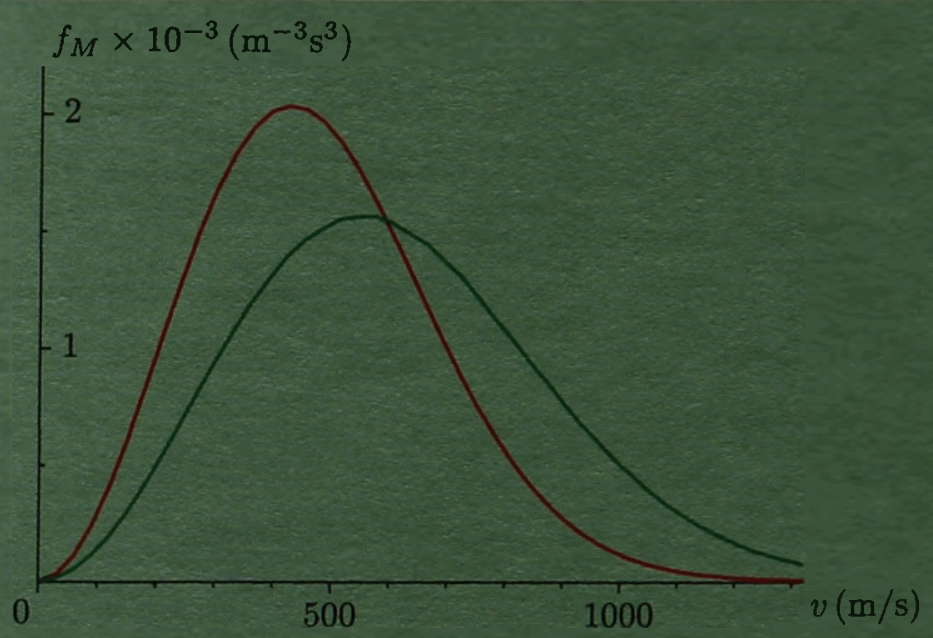
\includegraphics[width=0.4\linewidth]{mai_fig048.png}
   \captionof{figure}{Maxwellovo rozdělení rychlostí molekul dusíku pro teploty \(T_1 = 
                      \SI{300}{\kelvin}\) a \(T_2 = \SI{300}{\kelvin}\).
   \cite[s.~243]{Musilova2009MA1}
   \label{mai:fig048}}
  \par}
  
  Dokážete vyložit, proč jsme zvolili za \(\Delta\Omega\) celý objem slupky? Počítáme totiž 
  pravděpodobnost, že koncový bod vektoru rychlosti molekuly leží, zhruba řečeno, v kterémkoli 
  elementárním kvádříku \(\Delta v_x\Delta v_z\Delta v_z\) obsaženém ve slupce. A ta je součtem 
  pravděpodobností odpovídajících všem kvádříkům vytvářejícím slupku. Jedná se o pravděpodobnosti 
  navzájem neslučitelných jevů (pohybuje-li se molekula v jednom směru, nepohybuje se v jiném). 
  Hustota této pravděpodobnosti se nazývá \textbf{Maxwellovo rozdělení rychlostí}. Na rozdíl od 
  Gaussova rozdělení, popisujícího hustotu pravděpodobnosti pro jednotlivé složky rychlosti, je 
  nesymetrická vlivem faktoru \(v^2\). Obrázek \ref{mai:fig048} ukazuje funkci \(f_M(v)\) pro dvě 
  různé teploty \(T_2 > T_1\). Důležité hodnoty spjaté s tímto rozdělením jsou 
  \textbf{nejpravděpodobnější rychlost} \(v_p\), \textbf{střední rychlost} \(\langle v \rangle\) a 
  \textbf{střední kvadratická rychlost} \(\langle v^2 \rangle\). Platí
  \begin{align*}
    \der{f_M}{v}        &= 0\, \longrightarrow v_P = \sqrt{\dfrac{2kT}{m}},                      \\
    \langle v \rangle   &= \int_{-\infty}^{\infty}vf_M(v)\dd{v} = \sqrt{\dfrac{8kT}{\pi m}},     \\
    \langle v \rangle^2 &= \int_{-\infty}^{\infty}v^2f_M(v)\dd{v} = \dfrac{3kT}{m}.
  \end{align*}
\normalsize
\end{example}
      %---------------------------------------------------------------
  
  \section{Náhoda a zpracování měření}\label{mai:IchapIIIsecIV}
    \subsection{Součet a součin náhodných veličin}
      Nyní vyřešíme ještě jeden důležitý problém. Víme již, že veličinu \(Y = f(X)\) lze popsat 
      stejnými pravděpodobnostmi jako veličinu \(X\). V řadě případů je však náhodná veličina \(Y\) 
      funkcí několika náhodných veličin \(X_1, X_2, \ldots, X_s\). Každá z nich má nějaké 
      rozdělení. Jaké potom bude rozdělení veličiny \(Y\)? Rozebereme jen dvě základní situace, z 
      nichž je ovšem možné „poskládat“ řadu případů složitějších. Půjde o situace, kdy náhodná 
      veličina bude součtem nebo součinem dvou náhodných veličin, pro jednoduchost značení 
      například \(U\) a \(V\), tedy \(Y = U + V\), \(Z = U \cdot V\). Předpokládejme nejprve, že 
      veličiny \(U\) a \(V\) jsou zcela nezávislé, tj. hodnoty veličiny \(U\) nejsou nijak 
      ovlivněny hodnotami veličiny \(V\) a naopak. Dejme tomu, že \(U\) a \(V\) mají rozdělení
      \begin{equation*}
        \left\lbrace (u_1, p_1), \ldots, (u_k, p_k) \right\rbrace, \qquad
        \left\lbrace (v_1, q_1), \ldots, (v_\ell, v_\ell) \right\rbrace
      \end{equation*}
      Veličiny \(Y = U + V\), resp. \(Z = U \cdot V\) tedy mohou nabývat hodnot \(\lbrace u_i + 
      v_\alpha\rbrace\), resp. \(\lbrace u_i v_\alpha\rbrace\) s pravděpodobnostmi \(p_iq_\alpha\). 
      Jevy \uv{Veličina \(U\) nabude hodnoty \(u_i\)} a \uv{veličina \(V\) nabude hodnoty 
      \(v_\alpha\)} jsou totiž nezávislé. Rozdělení veličin \(Y\) a \(Z\) je 
      \begin{equation*}
        \lbrace (u_i +v_\alpha, p_iq_\alpha)\rbrace,\, \text{resp.}\,
        \lbrace(u_iv_\alpha, p_iq_\alpha)\rbrace,\qquad 1\leq i\leq k,\quad 1\leq\alpha\leq\ell,
      \end{equation*}
      Pro jejich střední hodnoty dostáváme
      \begin{align*}
        \langle y \rangle 
          &= \sum_{i=1}^{k}\sum_{\alpha=1}^{\ell}(u_i + v_\alpha)p_iq_\alpha
           = \sum_{i=1}^{k}u_ip_i\left(\sum_{\alpha=1}^{\ell}q_\alpha\right) + 
             \sum_{\alpha=1}^{\ell}v_\alpha q_\alpha\left(\sum_{i=1}^{k}p_i\right)  \\
          &= \sum_{i=1}^{k}u_ip_i + \sum_{\alpha=1}^{\ell}v_\alpha q_\alpha         \\
        \langle z \rangle 
          &= \sum_{i=1}^{k}\sum_{\alpha=1}^{\ell}(u_i \cdot v_\alpha)p_iq_\alpha
           = \left(\sum_{i=1}^{k}u_ip_i\right)
             \left(\sum_{\alpha=1}^{\ell}v_\alpha q_\alpha\right) 
           = \langle u \rangle \langle v \rangle.
      \end{align*}
      Střední hodnota součtu, resp. součinu náhodných veličin je tedy součtem, resp. součinem jejich
      středních hodnot. Pro součet náhodných veličin platí tento výsledek i v případě, když nebudou
      nezávislé. V tak jednoduchý závěr jsme snad ani nedoufali! Hned uvidíme, jak jej lze využít.
      
      %--Jak číst výsledky studentské ankety aneb není průměr jako průměr----------
      % !TeX spellcheck = cs_CZ
\wikitextrule
\begin{example}\label{mai:exam071}
  \textbf{Jak číst výsledky studentské ankety aneb není průměr jako průměr}\newline\small
  Každý semestr na Masarykově univerzitě se uzavírá vyhodnocením velmi užitečné studentské ankety v 
  Informačním systému MU. Studenti hodnotí na jedenáctihodnotové stupnici (nula až deset bodů) 
  několik položek pro každý studijní předmět (obtížnost, zajímavost, srozumitelnost výkladu, 
  přístup učitele, rozmanitost literatury) a mohou doplnit i slovní komentáře. Na ty se učitelé 
  těší nejvíce, neboť díky anonymitě pisatelů se tak o sobě mohou dovědět leccos zajímavého. 
  Všimneme si však statistického zpracování ankety. U každého předmětu je pro danou položku 
  vypočtena průměrná bodová hodnota odpovědí a vyznačena na téže jedenáctihodnotové stupnici. Pro 
  porovnání je na stupnici vyznačen i takzvaný „fakultní průměr“. Každý přednášející může vidět svá 
  hodnocení a hodnocení svých kolegů, kteří mu vedou cvičení. Děkan má přístupové právo k celé
  statistice, a tak může porovnávat. Jednoho deštivého večera přestalo děkana bavit vyplňování 
  rektorátních formulářů a začal si výsledky ankety prohlížet. Zajímala jej zejména položka 
  „srozumitelnost výkladu“. Řekl si, že všem učitelům, kteří v této položce budou hodnoceni 
  nadprůměrně, zvýší osobní ohodnocení. Soubor předmětů je veliký, a tak děkan klikal a klikal. 
  Zjišťoval, že u veliké většiny předmětů leží průměrné hodnocení srozumitelnosti nad fakultním 
  průměrem. Jeho pocity byly smíšené. Na jedné straně se radoval, jakými jsou jeho podřízení 
  dobrými pedagogy, na druhé straně trnul, kolik to bude stát. Snad aby se raději vrátil 
  k protivným formulářům. Najednou v něm zahlodalo podezření i naděje, že není všechno v pořádku. 
  Jak je možné, že většina hodnocení leží nad průměrem? Kladné a záporné odchylky by se přece měly 
  kompenzovat. Zavolal proto na koberec proděkana pro informační technologie, aby se jej zeptal, co 
  je to „fakultní průměr“. Proděkan odpověděl takto: Máme soubor \(K\) předmětů \(\lbrace 
  X_\alpha\rbrace\), \(\alpha = 1, \ldots, K\). V předmětu \(X_\alpha\) vyplnilo anketu 
  \(N_\alpha\)  studentů, jednotlivé hodnoty odpovědí pro danou položku (srozumitelnost výkladu) 
  byly označeny \(\lbrace x_{\alpha,j}\rbrace\), \(j = 1, \ldots, N_\alpha\). Celkem přirozeně 
  předpokládáme, že váha odpovědi každého studenta je stejná, nezávisle na předmětu. Tato váha je
  rovna převrácené hodnotě celkového počtu studentů, kteří vyplnili anketu, tj. \(w = N^{-1}\), \(N 
  = N_1 + \ldots + N_k\). Fakultní průměr je proto dán vzorcem
  \begin{equation*}
    \langle x \rangle 
      = \sum_{\alpha=1}^{K}\sum_{j=1}^{N_\alpha}wx_{\alpha,j} 
      = \dfrac{1}{N}\sum_{\alpha=1}^{K}\left(\sum_{j=1}^{N_\alpha}x_{\alpha,j}\right)
      = \dfrac{1}{N}\sum_{\alpha=1}^{K}A_\alpha,
  \end{equation*}
  kde jsme označili \(A_\alpha = \sum_{j=1}^{N_\alpha}x_{\alpha,j}\). Děkan chvíli přemýšlel a 
  pravil: To vypadá docela logicky. Neměli bychom však počítat fakultní průměr tak, že vezmeme 
  průměrné hodnoty pro každý předmět a vypočteme jejich aritmetický průměr? Pak bychom dostali
  \begin{equation*}
    \langle \overline{x} \rangle
      = \dfrac{1}{K}\sum_{\alpha=1}^{K}\langle x_{\alpha}\rangle
      = \dfrac{1}{K}\sum_{\alpha=1}^{K}
        \left(\dfrac{1}{N_\alpha}\sum_{j=1}^{N_\alpha}x_{\alpha,j}\right)
      = \dfrac{1}{K}\sum_{\alpha=1}^{K}\dfrac{A_\alpha}{N_\alpha}.
  \end{equation*}
  Tento závěr se akademickým funkcionářům na první pohled nijak zvlášť nelíbil. Bylo totiž jasné, 
  že náhodné veličiny \(X_1, \ldots, X_k\) mají odlišná rozdělení. No jo, řekli si oba, musíme 
  počítat. My už ale počítat nemusíme, neboť jsme takový problém před chvílí vyřešili obecně. 
  Zjistili jsme totiž, že střední hodnota součtu náhodných veličin je rovna součtu středních 
  hodnot, bez ohledu na konkrétní rozdělení každé z veličin. Definujeme-li tedy náhodnou veličinu 
  \(Y\) jako aritmetický průměr veličin \(X_\alpha\), tj.
  \begin{align*}
    Y &= \dfrac{1}{K}\left(X_1 + \ldots + X_K\right),  \\
    \shortintertext{dostaneme}
    \langle y \rangle &= \dfrac{1}{K}\left(\langle x_1 \rangle +\ldots+\langle x_K \rangle\right).
  \end{align*}
  Tento výsledek se shoduje s hodnotou \(\langle \overline{x} \rangle\), kterou pro výpočet 
  „fakultního průměru“ navrhl děkan. Vypočteme-li součet odchylek hodnot \(\langle x_\beta 
  \rangle\) od \(\langle y \rangle\), dostaneme skutečně nulu:
  \begin{equation*}
    \sum_{\beta =1}^{K}\left(\langle x_\beta \rangle - \langle y \rangle\right)
      = \sum_{\beta =1}^{K}\left(\dfrac{A_\beta}{N_\beta} 
      - \dfrac{1}{K}\sum_{\alpha=1}^{K}\langle x_\alpha \rangle\right)
      = 0.
  \end{equation*}
  Zkusme se ještě zamyslet nad tím , jak použití „špatného“ fakultního průměru zkreslilo výsledky a 
  proč. Vypočtěme si rozdíl \(\Delta = \langle \overline{x} \rangle - \langle x \rangle\):
  \begin{equation*}
    \Delta = \langle \overline{x} \rangle - \langle x \rangle 
      = \dfrac{1}{K}\sum_{\alpha=1}^{K}\langle x_\alpha \rangle
      - \dfrac{1}{N}\sum_{\alpha=1}^{K}A_\alpha
      = \dfrac{1}{K}\sum_{\alpha=1}^{K}\langle x_\alpha \rangle
      - \dfrac{1}{N}\sum_{\alpha=1}^{K}N_\alpha\langle x_\alpha \rangle
      = \dfrac{1}{K}\sum_{\alpha=1}^{K}\langle x_\alpha\rangle\left(1 - K\dfrac{N_\alpha}{N}\right).
  \end{equation*}
  Platí přitom
  \begin{equation*}
    \sum_{\alpha=1}^{K}\left(1 - K\dfrac{N_\alpha}{N}\right) = 0.
  \end{equation*}
  Pokud by byl počet studentů, kteří vyplnili anketu, ve všech předmětech stejný, tj. \(N_\alpha = 
  \dfrac{N}{K}\) , byla by odchylka \(\Delta\) podle očekávání nulová. Stejná situace by nastala, 
  kdyby byly shodné všechny průměrné hodnoty \(\langle x_\alpha \rangle\). Je-li odchylka 
  \(\Delta\) kladná, je „nesprávný“ fakultní průměr \(\langle x \rangle\) nižší než \(\langle 
  \overline{x} \rangle\). Proto hodnocení jednotlivých předmětů vypadají příznivěji, právě tak, jak 
  to zjistil děkan. Odchylku \(\Delta\) posouvají do kladných hodnot předměty, které hodnotilo málo 
  studentů, a předměty, které měly vysoké hodnocení. Dobře je to vidět na příkladu dvou předmětů, 
  tj. pro \(K = 2\), kde vychází
  \begin{equation*}
    \Delta = \langle \overline{x} \rangle - \langle x \rangle 
           = \dfrac{N_2 - N_1}{2(N_2+N_1)}\left(\langle\overline{x}\rangle-\langle x\rangle\right).
  \end{equation*}
  
  Pro \(N_1\ll N_2\) a \(\langle x_1 \rangle  \gg \langle x_2 \rangle \) bude rozdíl \(\Delta\) 
  skoro polovina hodnoty \(\langle x_1 \rangle\)! U volitelných specializovaných předmětů, které si 
  vybírají jen poměrně malé počty studentů, kteří navíc mají o předmět opravdový zájem a hodnotí 
  jej proto většinou vyšším počtem bodů, je splněno obojí (malý počet hodnotících a vysoké bodové
  hodnocení). Je vidět, že při nesprávně zvoleném výpočtu srovnávací hodnoty (fakultního průměru) 
  mohou právě předměty, jejichž statistický význam je spíše okrajový, ovlivnit celkové hodnocení.
\normalsize
\end{example}
      %----------------------------------------------------------------------------
      
      Pro střední hodnotu součtu a součinu nezávislých náhodných veličin jsme získali velmi
      jednoduché výsledky:
      
      \adjustbox{minipage=[c]{\textwidth}}{%
        \begin{equation}\label{mai:eq070}
          \langle u + v \rangle = \langle u \rangle + \langle v \rangle\qquad
          \langle uv \rangle    = \langle u \rangle \langle v \rangle.
        \end{equation}
      }
      
      Dokážeme také určit rozptyl veličin \(Y = U + V\) a \(Z = U\cdot V\)? Pro rozptyl každé 
      náhodné veličiny platí obecný vztah (\ref{mai:eq061}). Použijeme jej pro naše konkrétní 
      případy:
      \begin{align*}
        D(U + V) &= \langle (u + v)^2 \rangle - \langle u + v \rangle^2 
                  = \langle u^2 + 2uv + v^2 \rangle - \left(\langle u \rangle^2 +
                    \langle 2uv \rangle + \langle v^2 \rangle\right)                        \\
                 &= \left(\langle u^2\rangle - \langle u \rangle^2\right)
                  + \left(\langle v^2\rangle - \langle v \rangle^2\right) = D(U) + D(V).
      \end{align*}
      Pro rozptyl náhodné veličiny \(Z = U \cdot V\) dostaneme
      \begin{align*}
        D(Z)  &= \langle z^2\rangle - \langle z \rangle^2 
               = \langle u^2\rangle\langle v^2\rangle - \langle u \rangle^2 \langle v \rangle^2  \\
              &= \left[D(U) + \langle u^2\rangle\right]\left[D(V) + \langle v^2\rangle\right]
               - \langle u \rangle^2 \langle v \rangle^2                                         \\
              &= D(U)D(V) + \langle u \rangle^2D(V) + \langle v \rangle^2D(U).
      \end{align*}
      Pak
      \adjustbox{minipage=[c]{\textwidth}}{%
        \begin{equation*}
          \dfrac{D(z)}{ \langle z \rangle^2} = \dfrac{D(U)}{ \langle u \rangle^2} \cdot
            \dfrac{D(V)}{ \langle v \rangle^2} + \dfrac{D(U)}{ \langle u \rangle^2} +
            \dfrac{D(v)}{ \langle v \rangle^2}.
        \end{equation*}
      }
      Při výpočtu jsme využili vztahu (\ref{mai:eq061}) a vztahů (\ref{mai:eq070}) pro střední 
      hodnotu součtu a součinu náhodných veličin. Pokud mají veličiny \(U\) a \(V\) shodný rozptyl 
      \(D(U) = D(V) = D\), pak je \(D(U + V) = 2D\). V případě součtu s veličin \(Y = X_1 + \cdots 
      + X_s\) se shodným rozptylem \(D\) resp. směrodatnou odchylkou \(\sigma\) dostáváme
      \begin{equation*}
        D(Y) = sD  \Rightarrow \sigma(y) = \sqrt{s}\sigma.
      \end{equation*}
      Znovu připomeňme, že všechny vztahy týkající se součtu a součinu náhodných veličin, které
      jsme zatím získali, platí za předpokladu, že výchozí veličiny, které sčítáme nebo násobíme, 
      jsou nezávislé.
      
      Aniž bychom se podrobněji zabývali vlastnostmi rozdělení závislých veličin, definujeme pro
      ně charakteristiky, které tuto závislost popisují. Nechť \(U\) a \(V\) jsou dvě libovolně 
      náhodné veličiny, ne nutně nezávislé. Míru jejich závislosti určují veličiny
      \begin{equation}\label{mai:eq071}
        \sigma_{uv} = \langle (u - \langle u \rangle) (v - \langle v \rangle) \rangle, \qquad
        \varrho_ {uv}=\dfrac{\sigma(u)}{\sqrt{D(U)D(V)}} = \dfrac{\sigma(u)}{\sigma{D(u)\sigma(v)}}
      \end{equation}
      zvané \textbf{kovariance} a \textbf{korelační koeficient} veličin \(U\) a \(V\). Platí 
      \(\varrho(uv) \leq 1\). Pro nezávislé veličiny vychází \(\sigma(uv) = 0\) a \(\varrho(uv) = 
      0\).
      
      %-- Rozptyl při Bernoulliově pokusu-----------------------------
      % !TeX spellcheck = cs_CZ
\begin{mdframed}[style=mdexam]
  \begin{example}\label{mai:exam072}
    \textbf{Rozptyl při Bernoulliově pokusu}\newline
    V příkladu \ref{mai:exam066} jsme se zajímali o střední hodnotu veličiny \(X\) definované jako
    počet zdarů při \(n\) opakováních Bernoulliova pokusu. Řekli jsme si, že střední hodnota této
    veličiny je \(np\) s tím, že důkaz lze provést přímo na základě definičního vztahu pro střední
    hodnotu matematickou indukcí. Výpočet rozptylu z definičního vztahu bychom jistě snadno dokázali
    zahájit, horší by však bylo dovést jej do konce. Stačí se podívat na začátek výpočtu
    \begin{align*}
      D(X) &= \sum_{j=0}^n \left(x_j - \langle x \rangle\right)^2p_j             \\
           &= \sum_{j=0}^n \left(j - np\right)^2\binom{n}{j}p^j(1 - p)^j,
    \end{align*}
    a nepochybujeme o tom, že tuto sumu nedokážeme spočítat snadno. Protože již však umíme zacházet
    se součtem náhodných veličin, můžeme využít účinného triku. Veličinu \(X\) si představíme jako
    součet
    \begin{equation*}
      X = U_1 + U_2 + \cdots + U_n,
    \end{equation*}
    kde každá z veličin \(U_j\) může nabývat dvou hodnot. Jedničky v případě, že při \(j\)-tém
    opakování pokusu nastal zdar, a nuly v případě, že nastal nezdar. Součet všech veličin \(U_j\)
    pro \(j = 1\) až \(j = n\) pak skutečně znamená celkový počet zdarů při \(n\) opakováních
    pokusu. Jestliže si uvědomíme, že pravděpodobnost zdaru při kterémkoli z opakování je \(p\) a
    pravděpodobnost nezdaru \((1 - p)\), ihned vidíme, že rozdělení každé z veličin \(U_j\) má tvar
    \(\lbrace(1, p), (0, 1 - p)\rbrace\). Platí tedy
    \begin{equation*}
      \langle u_j\rangle = 1\cdot p + 0 \cdot (1 - p) = p,
    \end{equation*}
    \begin{align*}
      D = D(U_j) &= \left( 1 - \langle u_j\rangle\right)^2p 
                  + \left( 0 - \langle u_j\rangle\right)^2(1 - p)   \\
                 &= p(1 - p)^2 + p^2(1 - p) = p(1 - p).
    \end{align*}
    Každé dvě veličiny \(U_i\), \(U_j\) jsou nezávislé, neboť jednotlivá opakování pokusu jsou
    nezávislá. Střední hodnota jejich součtu je: tedy \(np\) (a to souhlasí s informací v příkladu
    \ref{mai:exam066}) a pro rozptyl jejich součtu platí
    \begin{equation*}
      D(X) = nD = np(1 - p).
    \end{equation*}
    Celkově tedy dostáváme
    \begin{equation*}
      \langle x \rangle = np, \; \sigma(x) = \sqrt{np(1 - p)}.
    \end{equation*}
  \end{example}
\end{mdframed}
      %---------------------------------------------------------------
      
      %-- Rozptyl aritmetického průměru-------------------------------
      % !TeX spellcheck = cs_CZ
\begin{mdframed}[style=mdexam]
  \begin{example}\label{mai:exam073}
    \textbf{Rozptyl aritmetického průměru}\newline
    Již v úvodu odstavce o náhodných veličinách jsme konstatovali, že opakujeme-li v nezměněných
    podmínkách měření jisté fyzikální veličiny (délka závěsu kyvadla, proud procházející vodičem,
    napětí na vodiči, atd.), budeme díky náhodným vlivům dostávat pokaždé poněkud jiný výsledek.
    Říkáme, že měření je zatíženo náhodnými chybami. Výsledek získaný při každém opakování lze
    interpretovat jako hodnotu náhodné veličiny. Dejme tomu, že jsme provedli uměření fyzikální
    veličiny \(X\) a získali hodnoty \(x_1\) až \(x_n\) . V praktické situaci budou tyto hodnoty
    většinou navzájem různé, nemusí tomu tak však nutně být. Fyzikální veličinu chceme ovšem
    reprezentovat jediným údajem, a tím bude její střední hodnota, tj.
    \textbf{aritmetický průměr}
    \begin{equation*}
      \langle x \rangle = \dfrac{x_1 + x_2 + \cdots + x_n}{n}.
    \end{equation*}
    Rozptyl veličiny \(X\) je dán vztahem
    \begin{align*}
      D &= D(X)                                                             \\
        &= \dfrac{\left(x_1 - \langle x \rangle\right)^2 + 
                  \left(x_2 - \langle x \rangle\right)^2 + \cdots +
                  \left(x_n - \langle x \rangle\right)^2}{n}.
    \end{align*}
    Víme, že směrodatná odchylka \(\sigma( x ) = \sqrt{D(X)}\) určuje, nakolik jsou jednotlivé
    výsledky měření v průměru odchýleny od střední hodnoty, charakterizuje tedy přesnost každého
    opakování měření. Podívejme se na celou úlohu z jiné strany: Představme si, že sledujeme \(n\)
    po dvou nezávislých náhodných veličin \(X_1\) až \(X_n\) se shodnou střední hodnotou \(\langle
    x_j \rangle = \langle x \rangle\) a shodnou směrodatnou odchylkou \(\sigma(x_j) = \sqrt{D},\, 1
    \leq j \leq n\). Aritmetický průměr těchto veličin,
    \begin{equation*}
      \langle \Xi \rangle = \dfrac{X_1 + X_2 + \cdots + X_n}{n}.
    \end{equation*}
    je tedy rovněž náhodnou veličinou. Pro jeho střední hodnotu, rozptyl a směrodatnou odchylku
    platí
    \begin{align*}
      \langle \xi \rangle 
                  &= \dfrac{n\langle x \rangle}{n}, \\
      D(\Xi)      &= \dfrac{1}{n^2}\cdot D(X_1 + \cdots + X_n)=\dfrac{nD^2}{n^2}=\dfrac{D}{n}, \\
      \sigma(\xi) &= \dfrac{\sigma(x)}{\sqrt{n}}.
    \end{align*}
  \end{example}
\end{mdframed}
      %---------------------------------------------------------------
      
      Můžeme tedy říci, že aritmetický průměr všech výsledků měření dané fyzikální veličiny je
      \(\sqrt{n}\)-krát přesnější než jednotlivý výsledek měření. Jakkoli se toto konstatování zdá 
      intuitivně zřejmé, je třeba je používat s opatrností.
      
      Především je třeba mít na mysli, co toto konstatování znamená. Jeho charakter je totiž
      opět jen pravděpodobnostní. Jestliže jsou jednotlivá měření prováděna za stejných podmínek,
      jsou rozdělení veličin \(X_1\) až \(X_n\) funkcemi téhož typu. Tyto veličiny mají také 
      stejnou střední hodnotu \(\langle x \rangle\) a směrodatnou odchylku \(\sigma\). Také 
      pravděpodobnost, že při měření padne hodnota veličiny \(X_j\) do intervalu \((\langle x 
      \rangle - \sigma, \langle x \rangle + \sigma)\), je pro všechna \(j\) prakticky stejná. 
      Označme ji \(P_\sigma\).  Se stejnou pravděpodobností nabude aritmetický průměr \(\Xi\) 
      hodnoty v intervalu určeném svou směrodatnou odchylkou. Ta je však \(\sqrt{n}\)-krát menší. V 
      tomto smyslu jsou hodnoty aritmetického průměru \uv{\(\sqrt{n}\)-krát méně rozptýleny} kolem 
      střední hodnoty \(\langle\xi \rangle\) než hodnoty náhodných veličin \(X_j\) kolem svých 
      středních hodnot \(\langle x \rangle\).
      
      Dalším problémem může být splnění výchozích předpokladů, které vedly ke vztahu pro
      směrodatnou odchylku aritmetického průměru. Ukážeme to na následujícím příkladu.
      
      %-- Jak přesně lze změřit čínského císaře?----------------------
      % !TeX spellcheck = cs_CZ
\wikitextrule
\begin{example}\label{mai:exam075}
  \textbf{Ověření Ohmová zákona}\newline\small

\normalsize
\end{example}
      %---------------------------------------------------------------
      
      %-- Záhada přijímací zkoušky aneb k čemu může posloužit distribuční funkce-----
      % !TeX spellcheck = cs_CZ
\begin{mdframed}[style=mdexam]
  \begin{example}\label{mai:exam075}
    \textbf{Záhada přijímací zkoušky aneb k čemu může posloužit distribuční funkce?}\newline
    Mohlo by se zdát, že distribuční funkce je jen teoretický pojem a že v praktických situacích ji
    těžko využijeme. Podstatné je přece pravděpodobnostní rozdělení náhodné veličiny a distribuční
    funkce je z něj jen jaksi odvozena sčítáním pravděpodobností (u diskrétního rozdělení) nebo
    integrací (u rozdělení spojitého). Přesvědčíme se, že existují velmi realistické případy, kdy
    distribuční funkce přináší věrohodnější informaci o náhodné veličině než samotné rozdělení.
    
    Na Masarykově univerzitě musí každý uchazeč o studium, ať již se hlásí na přírodovědeckou,
    právnickou, lékařskou či jinou fakultu, absolvovat Test studijních předpokladů. Jedná se o
    všeobecný test, zaměřený na zjišťování úrovně všech schopností uchazeče, které jsou potřebné pro
    univerzitní studium, například analytického myšlení, verbálních schopností, numerického myšlení,
    geometrické představivosti, atd. Pro nás však v tu to chvíli není podstatný obsah testu, ale
    způsob zpracování jeho výsledků a vyhodnocení pořadí uchazečů. Test skládá kolem třiceti tisíc
    studentů. Není tedy možné technicky zajistit, aby proběhl v jediné variantě v jednom dni. K
    dispozici je proto osm variant testu, každou variantu řeší tři až čtyři tisíce studentů. Test má
    \num{80} otázek, základním údajem pro zpracování jeho výsledků je počet správných odpovědí
    každého studenta. Pokud bychom označili jako \(i\) počet správných odpovědí (\(i \in\lbrace0, 1,
    2, \ldots, 80\rbrace\)) v kterékoli variantě a \(\mathcal{N}_i\) počet studentů, kteří dosáhli
    právě \(i\) správných odpovědí, dostaneme náhodnou veličinu \(X_i\), kterou bychom mohli nazvat
    „počet správných odpovědí“, pro celou univerzitu. Její rozdělení by mělo tvar
    \begin{equation*}
      \lbrace(i,p_i)\rbrace,\quad\text{kde}\qquad p_i = \dfrac{\mathcal{N}_i}{\mathcal{N}}, \quad
      \mathcal{N} = \sum_{i=0}^{80}\mathcal{N}_i
    \end{equation*}
    A zde je malý „kámen úrazu“. A by bylo možné sestavit opravdu „univerzální pořadí“, musely by
    být všechny varianty testu ekvivalentní z hlediska obtížnosti. To znamená, že kdyby kterýkoli
    student vyplnil za stejných podmínek všechny varianty, dosáhl by v každé z nich stejného počtu
    správných odpovědí s pravděpodobností velmi blízkou jedné. Skutečnost je však principiálně
    taková, že u sebelépe promyšleného a sestaveného testu se jednotlivé varianty budou mírně, v
    rámci statistických, a tedy již neodstranitelných, odchylek lišit. Tato odlišnost se nepozná
    předem, ale až po zpracování výsledků všech variant. Použít pro stanovení pořadí uchazečů
    rozdělení náhodné veličiny \(X\) \emph{= počet správných odpovědí je tedy nespravedlivé}.
    Student, který řešil variantu „statisticky obtížnější“, by v pořadí skončil s horším umístěním,
    než student, který je stejně schopný, avšak měl to štěstí, že na něj připadla varianta
    „statisticky méně obtížná“. Skutečně, kdybychom sestavili grafy rozdělení náhodných veličin
    \(X^{(\alpha)}\) \emph{= počet správných odpovědí v \(\alpha\)-té variantě},
    \begin{equation*}
      \lbrace(i,p_i^{(\alpha)})\rbrace,\quad\text{kde}\; 
      p_i^{(\alpha)} = \dfrac{\mathcal{N}_i^{(\alpha)}}{\mathcal{N}^{(\alpha)}}, \quad
      \mathcal{N}^{(\alpha)} = \sum_{i=0}^{80}\mathcal{N}_i^{(\alpha)}
    \end{equation*}
    zjistili bychom, že se mírně liší. (V předchozím zápisu značí \(\mathcal{N}_i^{(\alpha)}\) počet
    studentů, kteří odpověděli správně na \(i\) otázek \(\alpha\)-té varianty
    \(\mathcal{N}^{(\alpha)}\) je počet všech studentů, kteří tuto variantu řešili.) Střední hodnoty
    i mediány náhodných veličin se i při vynikající shodě obtížnosti všech variant mohou lišit v
    rozmezí jedné až dvou správných odpovědí. A s ohledem na skutečnost, že každou variantu řeší
    obrovský počet studentů, až čtyři tisíce, je zřejmé, že tento rozdíl může poněkud „zamíchat
    “pořadím, zejména v blízkosti mediánu, kde se týká třeba i tří stovek studentů v každé variantě.
    Situaci dokládá obrázek \ref{mai:fig049}. Jak tedy zařídit, abychom dostali spravedlivé pořadí?
    Jediný rozumný způsob, jak minimalizovat vliv statistických odchylek obtížnosti jednotlivých
    variant, je nehodnotit studenty podle absolutního počtu správných odpovědí, ale nějak je
    porovnat mezi sebou. Budeme při tom předpokládat, že rozložení schopností studentů je ve všech
    osmi skupinách, které řeší osm daných variant, stejné. Řeknete si - zase nějaké další
    předpoklady. To je jako z bláta do louže. Předpoklad o stejném rozložení schopností studentů v
    tak velkých skupinách, jako jsou ty naše, je však mnohem realističtější než předpoklad o
    dokonalé shodě obtížnosti variant testu. Budeme se jej proto držet. Každému studentovi
    přisoudíme číslo, které informuje o tom, kolik řešitelů dané varianty bylo horších nebo stejně
    dobrých jako on, tj. mělo nižší nebo stejný počet správných odpovědí. Z matematického hlediska
    to znamená přejít v každé variantě od rozdělení k distribuční funkci. Věnujme se nyní tomuto
    přepočtu podrobněji jak pro diskrétní rozdělení náhodné veličiny \(X^{(\alpha)}\), které
    odpovídá skutečné situaci, tak pro zajímavost i pro rozdělení spojité. V dalším budeme vždy
    zpracovávat výsledky jedné varianty, upustíme proto od vyznačování indexu \(\alpha\).

    {\centering
    \captionsetup{type=figure}
    \luafigure[0.8]{mai_fig049.png}
    \captionof{figure}{Rozdělení pro dvě varianty testu,
    \cite[s.~252]{Musilova2009MA1}
    \label{mai:fig049}}
    \par}
    
    \textbf{Diskrétní rozdělení}
      \begin{itemize}
        \item \emph{Zadání:} Skupina \(N\) studentů řeší jednu variantu testu. Test má \(Q\) otázek.
              Za každou správnou odpověď je přidělen jeden výchozí bod. Získáváme rozdělení
              \begin{gather*}
                \left\lbrace\left(i, \dfrac{N_i}{N} \right)\right\rbrace, \;
                i\in\lbrace0, 1, 2, \ldots, Q\rbrace, \;
                \sum_{i=0}^{Q}N_i = N 
              \end{gather*}
              kde \(i\) je počet výchozích bodů a \(N_i\) počet studentů, kteří získali \(i\) bodů.
              Distribuční funkce tohoto rozdělení
              \begin{gather*}
                F(x) = \dfrac{1}{N}\sum_{i=0}^{j}N_i\;\text{ pro }\;
                j\leq x < j+1, \; x\in\left[0,\infty\right)
              \end{gather*}
              Pro uchazeče, který získal \(j\) bodů, mají význam následující hodnoty:
              \begin{itemize}
                \item \(F(x)    x \in \left[j, j+1\right)\): poměrný počet uchazečů, kteří získali
                      počet výchozích bodů nižší nebo shodný s daným uchazečem,
                \item \(NF(x)   x \in \left[j, j+1\right)\): absolutní počet uchazečů, kteří získali
                      počet výchozích bodů nižší nebo shodný s daným uchazečem,
                \item \(100F(x) x \in \left[j, j+1\right)\): absolutní počet uchazečů, kteří získali
                      počet výchozích bodů nižší nebo shodný s daným uchazečem,
              \end{itemize}
        \item Hodnoty distribuční funkce můžeme získat z následující tabulky:
        
              {\centering
                \resizebox{0.8\textwidth}{!}{%
                \begin{tabular}{c|c}
                          interval \(x\)     &  \(NF(x)\)         \\ \hline
                  \(\left[0,1\right)\)       &  \(N_0\)           \\ 
                  \(\left[1,2\right)\)       &  \(N_0 + N_1\)     \\ 
                  \(\cdots\)                 &  \(\cdots\)        \\
                  \(\left[j,j+1\right)\)     &  \(N_0 + N_1 + \cdots + N_j\) \\ 
                  \(\cdots\)                 &  \(\cdots\) \\
                  \(\left[Q-1,Q\right)\)     &  \(N_0 + N_1 + \cdots + N_{Q-1}\) \\ 
                  \(\left[Q,\infty\right)\)  &  \(N_0 + N_1 + \cdots + N_{Q} = N\) 
                \end{tabular}}
              \par}
        \item Přepočet hodnocení uchazečů tak, aby nová stupnice byla opět v rozsahu mezi nulou a
              \(Q\) a aby nové hodnocení bylo opět celočíselné, je následující:
              \begin{equation*}
                y =QF(x), \quad 0\leq F(x) \leq 1, \Rightarrow y \in[0,Q].
              \end{equation*}
              Uchazeči se ziskem \(i\) výchozích bodů náleží hodnota \(y = QF(x)\) právě když i\(
              \in \left[i, i + 1\right)\), tj. \(y_i = Q F(i)\). Tato hodnota není obecně
              celočíselná. Zaokrouhlení se provede ve prospěch uchazeče, tedy vždy nahoru. Výsledný
              převodní vzorec je
              \begin{equation*}
                \begin{multlined}
                  \text{výchozí body } i \longrightarrow\text{ nové body }  \\ 
                  \shoveleft[1cm]Y_i: Y_i = [y_i] + 1 = [QF(i)] + 1,
                \end{multlined}
              \end{equation*} 
              kde \([a]\) značí celočíselnou část čísla \(a\), tedy například \([\num{23.05}] =
              [\num{23.48}] = [23,89] = 23\)
        \item Zaveďme novou náhodnou veličinu \(Z\) s rozdělením \(\left\lbrace(z_\alpha,
              M_\alpha)\right\rbrace\): Označme \(z_1, z_2, \ldots, z_\alpha, ...,\) \(z_S\)
              navzájem různé hodnoty ze souboru \(\lbrace Y_i\rbrace, i = 0, 1, 2, \ldots, Q\)
              řazené vzestupně. Její rozdělení udává kterákoli z následujících tabulek:

              {\centering
                \resizebox{0.9\textwidth}{!}{%
                \begin{tabular}{c|c}
                          hodnota                       &  četnost         \\
                          \hline
                  \(z_1 = Y_0 = Y_1 = \cdots Y_{i_1}\)  & \(M_1 = N_0 + N_1 + \cdots + N_{i_1}\)  \\ 
                  \(Z_2 = Y_{i_1+1} = \cdots Y_{i_2}\)  & \(M_2 = N_{i_1+1} + \cdots + N_{i_2}\)  \\ 
                  \(\cdots\)                            & \(\cdots\)                              \\
                  \(Z_S = Y_{i_{S-1}+1}=\cdots Y_{i_S}\)& \(M_S = N_{i_{S_1}+1}+\cdots+N_{i_S}\)   
                \end{tabular}}
              \par}

              {\centering
                \resizebox{0.9\textwidth}{!}{%
                \begin{tabular}{c|c}
                          hodnota                        &  četnost         \\
                          \hline
                  \(z_1 = Y_0 = Y_1 = \cdots Y_{i_1}\)   &  \(M_1 = NF(i_1)\)              \\
                  
                  \(Z_2 = Y_{i_1+1} = \cdots Y_{i_2}\)   &  \(M_2 = N[F(i_2) - F(i_1)]\)  \\ 
                  \(\cdots\)                             &  \(\cdots\)                     \\
                  \(Z_S = Y_{i_{S-1}+1}=\cdots Y_{i_S}\) & \(M_S = N[F(i_S) - F(i_{S-1})]\)   
                \end{tabular}}
              \par}
              kde \(i_1 < i_2 < \ldots < i_{S-1} < i_S, i_S = Q\) (Vzhledem k zaokrouhlování nahoru
              není žádná bodová hodnota \(Y_i\) nulová.) I když skutečné rozdělení při zpracování
              výsledků testů je diskrétní, ukažme si, jak by vypadal analogický postup u rozdělení
              spojitého, kde je početní zpracování názornější.
      \end{itemize}
    
    \textbf{Spojité rozdělení}
      \begin{itemize}
        \item \emph{Zadání:} Je dáno rozdělení četností \(n(x) \leq 0,\, x \in [0, Q]\).
        \item Normovací podmínka a distribuční funkce jsou
              \begin{equation*}
                \int_{0}^{Q}n(x)\dd{x} = N, \quad 
                F(x) = \dfrac{1}{n}\int_{0}^{x}n(\xi)\dd{\xi},                
              \end{equation*}
              kde \(0 \leq F(x) \leq 1.\)
        \item Označme \(z = QF(x)\), tedy \(z \in [0, Q]\), novou náhodnou veličinu. (Uvědomme si,
              že \(z\) je rostoucí funkcí proměnné \(x\)). Označme její rozdělení \(\nu(z)\). Její
              distribuční funkce je
              \begin{align*}
                \Phi(z) &= \int_{0}^{z}\nu(\zeta)\dd{\zeta} 
                         = \int_{0}^{x(z)}\dfrac{n(\xi)}{N}\dd{\xi}          \\
                        &= F\left(F^{-1}(z/Q)\right) 
                        = \dfrac{z}{Q}, \quad
                \nu(z) = \dfrac{1}{Q}.
              \end{align*}
        \item Rozdělení je konstantní s mediánem i střední hodnotou \(Q/2\). Takové rozdělení se
              nazývá rovnoměrné.
      \end{itemize}
  \end{example}
\end{mdframed}
      %------------------------------------------------------------------------------
      
    \subsection{Který výsledek je ten pravý?}
      První věc, kterou budete dělat ve fyzikálním praktiku, bude zjišťování průměrné hustoty 
      materiálu, z něhož je vyroben kovový váleček. Budete váleček vážit, abyste určili jeho 
      hmotnost,a měřit jeho výšku a průměr, abyste mohli vypočítat jeho objem. Hustotu stanovíte 
      jako podíl hmotnosti a objemu. Jedná se stále o jeden a týž váleček, jehož průměrná hustota 
      má za daných podmínek (stálá teplota, váleček se nedeformuje, apod.) stále stejnou „správnou“ 
      hodnotu, kterou však neznáme. (Nezná ji ani učitel v praktiku, i když se tak tváří.) Změří-li 
      hustotu válečku všichni studenti ve skupině, každý jen jednou, získá se řada různých hodnot. 
      Která z nich je ta správná? Není vyloučeno, a je to dokonce velmi pravděpodobné, že žádná. A 
      mohli bychom pomocí nich správnou hodnotu určit nebo se k ní alespoň přiblížit? Možné by to 
      bylo, pokud bychom zaručili, že všechny výsledky získané jednotlivými studenty jsou „stejně 
      hodnotné“. Znamenalo by to, že bychom museli vyloučit hrubé a systematické chyby, které by 
      vznikly třeba tak, že by někteří studenti vážili na vadných vahách, někteří by měli špatné 
      měřítko, popřípadě by odečítali údaj „zboku“, takže by byl zkreslený, nebo by se dokonce 
      zmýlili při odečítání údaje. Museli bychom také zaručit, že náhodné vlivy, které ovlivňují 
      měření, zatěžují je náhodnými chybami a v principu je nelze odstranit, byly při všech 
      měřeních stejné. U různých studentů si tím však nemůžeme být jisti (vzpomeňte si na měření 
      čínského císaře), proto budeme raději postupovat tak, že jeden pečlivý student provede větší 
      počet měření třeba výšky válečku, která je pro určení hustoty potřebná. Dejme tomu, že bude 
      měřit milimetrovým měřítkem a bude odhadovat s přesností na půl milimetru. Jeho údaje tedy 
      mohou mít tvar \SI{33.0}{\mm}, \SI{34.5}{\mm}, atd. Získá takto za stejných podmínek třeba 
      dvacet nebo i padesát hodnot, ale co teď s nimi? Jak určit hodnotu, která se bude nejvíce 
      blížit správné hodnotě výšky válečku? (Dalo by se jistě diskutovat i o tom, co je to správná 
      hodnota. Pro tuto chvíli však předpokládejme, že taková hodnota skutečně existuje, neboť 
      váleček je opravdu válcem, je vysoustružen pečlivě, přesněji, než jsme schopni jej měřit, při 
      měření se nemění teplota, váleček není dáván do lisu a deformován, ani upravován tak, že by 
      se měnila jeho hmotnost.) Předpokládejme, že správná hodnota výšky válečku je \(x\) a že 
      student naměřil hodnoty \(\lbrace x_1, X_2, \ldots, x_n\rbrace\), mezi nimiž mohou být 
      pochopitelně i některé hodnoty stejné. Odchylky jeho měření od správné hodnoty jsou
      \begin{equation*}
        \lbrace \varepsilon_1, \varepsilon_2, \ldots, \varepsilon_n\rbrace, \qquad
        \varepsilon_i = x_i - x, \qquad i = 1, 2, \ldots, n.
      \end{equation*}
      I kdybychom správnou hodnotu \(x\) znali, nedokázali bychom předpovědět, nakolik se od ní při
      jednotlivém měření odchýlíme. Můžeme, se však zajímat o to, jaká je pravděpodobnost, že
      hodnota, o kterou bude měření od správné hodnoty odkloněno, bude ležet v určitém intervalu.
      Odchylky \(\varepsilon_i\) lze totiž interpretovat jako hodnoty náhodné veličiny. Abychom 
      mohli požadované pravděpodobnosti určit, potřebujeme znát rozdělení této veličiny. Označme ji 
      \(\varepsilon\) a odpovídající hustotu pravděpodobnosti \(\mathcal{w}(\varepsilon)\). Toto 
      rozdělení je za určitých podmínek \textbf{rozdělením normálním}, splňuje tedy vztah 
      (\ref{mai:eq069}). Zkusme se o tom přesvědčit. Zvolme podmínky měření tak, aby byly ve hře 
      jen náhodné chyby způsobené \(m\) nezávislými vlivy. Každý z nich hodnotu měření
      odchýlí od \(x\) o stejně velkou hodnotu \(\alpha\), kladnou nebo zápornou, s 
      pravděpodobností \num{0.5}. Schéma této úvahy je na obrázku \ref{mai:fig050}. Výsledná 
      odchylka naměřené hodnoty \(x_i\) od hodnoty správné s jistotou leží v intervalu \((-m\alpha, 
      m\alpha)\) a může nabývat pouze hodnot celých násobků \(\alpha\). Při uplatnění jednotlivého 
      „chybového“ vlivu vzniká, jak jsme již řekli, kladná nebo záporná odchylka o velikosti 
      \(\alpha\). Vznik odchylky \(+\alpha\) nazveme zdarem, vznik odchylky \(-\alpha\) nezdarem.
      
      \begin{figure}[ht!] %\ref{mai:fig050}
        \centering
        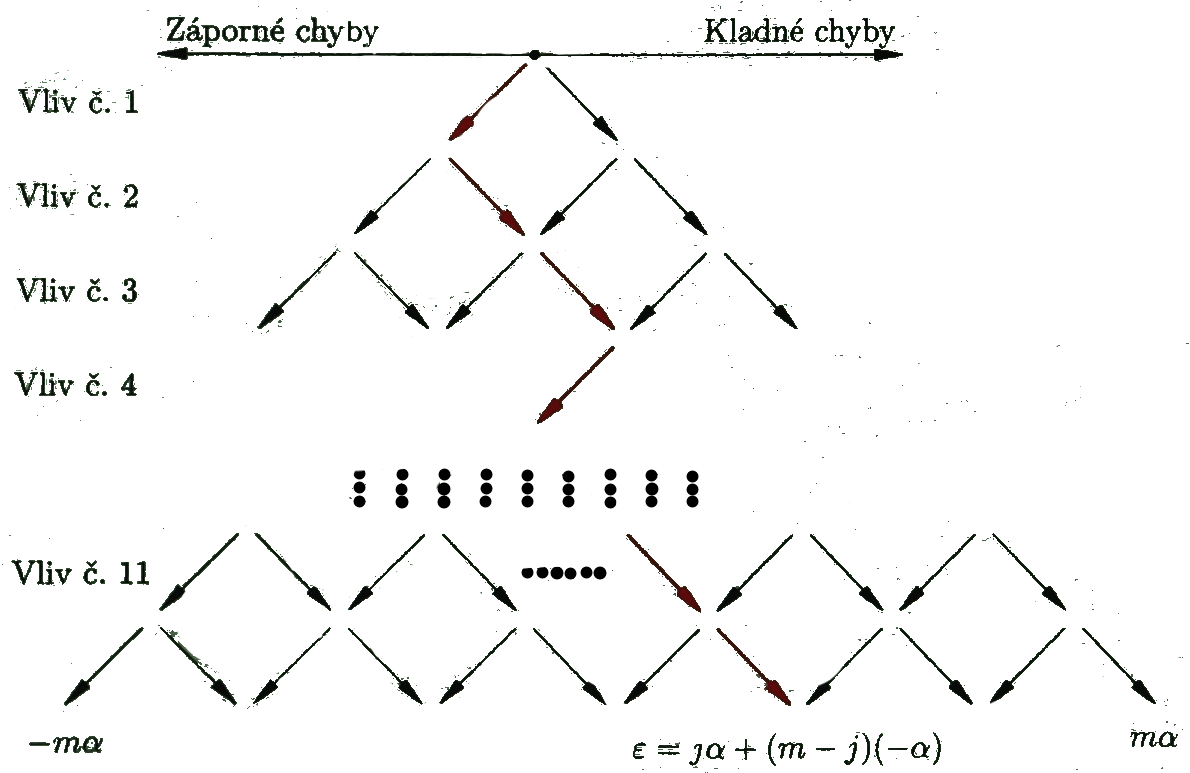
\includegraphics[width=0.6\linewidth]{mai_fig050.png}
        \caption{Vznik kladných a záporných odchylek při měření s \(m\) vlivy. 
        \cite[s.~255]{Musilova2009MA1}}
        \label{mai:fig050}
      \end{figure}
      
      Mohlo by tomu být i naopak, slova „zdar“ a „nezdar“ zde nemají svůj obvyklý význam, jde
      pouze o to, že díky nim můžeme hned uvidět souvislost s Bernoulliovým pokusem a tedy
      i s Bernoulliovým rozdělením. Při \(j\) kladných a \(m — j\) záporných odchylkách je měření od
      správné hodnoty odkloněno o
      \begin{equation*}
        j\alpha + (m - j)(-\alpha) = (2j - m)\alpha
      \end{equation*}
      s pravděpodobností
      \begin{equation*}
        p_j = \begin{pmatrix}m j\end{pmatrix}p^j(1 - p)^{m - j} = 2^{-m}.
      \end{equation*}
      Střední hodnota náhodné veličiny \(\varepsilon\) je nulová. Skutečně, v příkladu 
      \ref{mai:exam066} jsme zjistili, že střední hodnota veličiny \(Y\) nabývající hodnot \(y_j = 
      j\) s Bernoulliovým rozdělením je \(\langle y \rangle = mp\), střední hodnota veličiny \((2j 
      — m)\) a pak musí být \((2mp — m)\alpha\). Pro \(p = \num{0.5}\) je tato hodnota nulová.
      Pro velká \(m\) lze Bernoulliovo rozdělení nahradit rozdělením normálním (obr. 3.8), a proto 
      má náhodná veličina \(\varepsilon\) hustotu pravděpodobnosti tvaru (\ref{mai:eq069}), tj.
      \begin{equation*}
        \mathcal{w}(\varepsilon) = 
        \dfrac{1}{\sigma\sqrt{2\pi}}\exp\left(\dfrac{-\varepsilon^2}{2\sigma^2}\right).   
      \end{equation*}
      \begin{figure}[ht!] %\ref{mai:fig051}
        \centering
        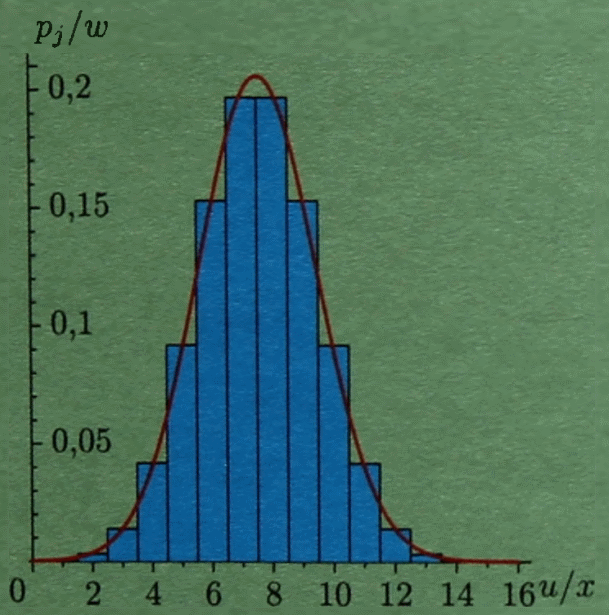
\includegraphics[width=0.4\linewidth]{mai_fig051.png}
        \caption{Normální rozdělení jako limitní případ Bernoulliova 
        \cite[s.~256]{Musilova2009MA1}}
        \label{mai:fig051}
      \end{figure}
      
      Vraťme se nyní k otázce zpracování naměřených hodnot \(\lbrace x_1, \ldots, x_n\rbrace\) 
      výšky válečku. Jejich odchylky od správné hodnoty jsou \(x_1 - x\) až \(x_n - x\). Na místě 
      neznámé správné hodnoty \(x\) si nyní představme nějakou proměnnou, označme ji 
      \(\varepsilon\). Budeme se snažit určit její hodnotu \(\varepsilon_0\) tak, aby 
      pravděpodobnost, že odchylky jednotlivých měřených hodnot od \(\varepsilon_0\) padnou 
      současně do intervalů
      \begin{equation*}
        \left(\varepsilon_1 - \dfrac{\dd{\varepsilon_1}}{2}, 
              \varepsilon_1 + \dfrac{\dd{\varepsilon_1}}{2}
        \right),
        \left(\varepsilon_2 - \dfrac{\dd{\varepsilon_2}}{2}, 
              \varepsilon_2 + \dfrac{\dd{\varepsilon_2}}{2}
        \right), \cdots,
        \left(\varepsilon_n - \dfrac{\dd{\varepsilon_n}}{2}, 
              \varepsilon_n + \dfrac{\dd{\varepsilon_n}}{2}
        \right),
      \end{equation*}
      byla maximální. Pro tuto pravděpodobnost v závislosti na \(\xi\) platí
      \begin{align}
        \dd{W} &= \dd{\mathcal{w}(\varepsilon_1)}\cdots\dd{\mathcal{w}(\varepsilon_n)}  \nonumber\\
               &= \dfrac{1}{\sigma\sqrt{2\pi}}
                  \exp\left(-\dfrac{(x_1 - \xi)^2 + \cdots + (x_n - \xi)^2}{2\sigma^2}
                      \right)\dd{\varepsilon_1}\cdots\dd{\varepsilon_n}.      \label{mai:eq072}
      \end{align}
      (Víte proč je ve vztahu (\ref{mai:eq072}) součin pravděpodobností?) Tato pravděpodobnost bude 
      maximální, bude-li hodnota exponentu minimální. Z podmínky
      \begin{equation*}
        (x_1 - \xi)^2 + \cdots + (x_n - \xi)^2 = \text{min}
      \end{equation*}
      dostáváme derivací podle \(\xi\) požadavek
      \begin{equation*}
        2(x_1 - \xi) + \cdots + 2(x_n - \xi) = 0 \Rightarrow \xi_0 = 
        \dfrac{1}{n}\sum_{i=1}^{n}x_j = \langle x \rangle.
      \end{equation*}
      Vidíme, že veličina, která charakterizuje míru odchýlení naměřených hodnot od \(\xi\), je 
      minimální, zvolíme-li za \(\xi\) aritmetický průměr naměřených hodnot. Pozor, zjištěný 
      výsledek znamená právě jen konstatovanou skutečnost: Při dosazení aritmetického průměru za 
      proměnnou \(\xi\) bude pravděpodobnost, že odchylky jednotlivých měření od \(\xi\) budou 
      ležet v uvažovaných intervalech, maximální. Neznamená to, že správnou hodnotou veličiny \(X\) 
      je aritmetický průměr měření \(x_1, X_2, \ldots, x_n\). Správnou hodnotu ze souboru měření 
      prostě nezjistíme, avšak aritmetický průměr je jí blízký s vysokou pravděpodobností. Jaká je 
      tato „blízkost“ a její pravděpodobnost konkrétně? Hned uvidíme. Správnou hodnotu výšky 
      válečku \(x\) sice neznáme, ale víme, že náhodná veličina \(\varepsilon\), jejíž hodnoty jsou 
      odchylkami výsledků měření od této (neznámé) správné hodnoty, se řídí normálním rozdělením s 
      nulovou střední hodnotou. Potřebujeme stanovit další důležitý parametr tohoto rozdělení, 
      směrodatnou odchylku \(\sigma\). Tu lze vyjádřit velmi jednoduše. Je totiž střední hodnotou 
      náhodné veličiny \(\varepsilon^2\), tedy aritmetickým průměrem čtverců odchylek 
      \(\varepsilon_i\): 
      \begin{equation*}
        \sigma^2 = D(\varepsilon) = \dfrac{1}{n}\sum_{i=1}^{n}\varepsilon_i^2.
      \end{equation*}
      Ať je však tento vzorec jakkoli jednoduchý, k čemu může sloužit, nedokážeme-li jej vyčíslit?
      Když přece neznáme správnou hodnotu \(x\), nemáme k dispozici ani hodnoty \(\varepsilon_i\). 
      Ani tato kaše však není tak horká, jak se zdá: Odchylku výsledku \(i\)-tého měření od 
      aritmetického průměru označme \(\delta_i = x_i - \langle x \rangle\), přičemž jsme již dříve 
      označili jako \(\varepsilon_i= x_i - x\) odchylku výsledku \(i\)-tého měření pd správné 
      hodnoty. Platí
      \begin{equation*}
        \sum_{i=1}^{n}\varepsilon_i = \sum_{i=1}^{n}(x_i - x) \Rightarrow 
        \sum_{i=1}^{n}x_i = \sum_{i=1}^{n}\varepsilon_i + nx, 
      \end{equation*}
      odkud 
      \begin{equation*}
        \langle x \rangle = x + \dfrac{1}{n}\sum_{i=1}^{n}\varepsilon_i.
      \end{equation*}
      Pak dostaneme
      \begin{equation*}
        \delta_i = (x_i - x) - \dfrac{1}{n}\sum_{i=1}^{n}\varepsilon_i 
                 = \varepsilon_i - \dfrac{1}{n}\sum_{j=1}^{n}\varepsilon_j.
      \end{equation*}
      Součet čtverců odchylek \(\delta_i\) je
      \begin{align*}
        \sum_{i=1}^{n}\delta_i^2 
          &= \sum_{i=1}^{n}\left(\varepsilon_i - 
             \dfrac{1}{n}\sum_{j=1}^{n}\varepsilon_j\right)^2 = \sum_{i=1}^{n}\varepsilon_i^2 - 
             \dfrac{2}{n}\sum_{i=1}^{n}\sum_{j=1}^{n}\varepsilon_i\varepsilon_j + 
             \dfrac{1}{n^2}\sum_{i=1}^{n}\left(\sum_{j=1}^{n}\varepsilon_j\right)^2     \\
          &= \sum_{i=1}^{n}\varepsilon_i^2 - 
             \dfrac{1}{n}\left(\sum_{j=1}^{n}\varepsilon_j\right)^2                     
             \doteq \left(1 - \dfrac{1}{n}\right)\sum_{i=1}^{n}\varepsilon_i^2.
      \end{align*}
      Při poslední úpravě jsme pro získání výsledného přibližného vyjádření součtu čtverců odchylek
      \(\delta_i\) použili následující úvahy:
      \begin{equation*}
        \left(\sum_{j=1}^{n}\varepsilon_j\right)^2 = \sum_{i=1}^{n}\varepsilon_i^2 + 
        2\sum_{i=1}^{n}\sum_{j>1}\varepsilon_i\varepsilon_j \doteq \sum_{i=1}^{n}\varepsilon_i^2,
      \end{equation*}
      neboť při rovnocenném zastoupení kladných a záporných odchylek je druhý sčítanec, obsahující
      součiny \(\varepsilon_i\varepsilon_j\), zanedbatelný proti prvnímu. Nakonec tedy dostáváme
      \begin{equation*}
        \sum_{i=1}^{n}\delta_i^2 \doteq \dfrac{n-1}{n}\sum_{i=1}^{n}\varepsilon_i^2 = (n-1)\sigma^2.
      \end{equation*}
      Protože odchylky \(\delta_i\) již z daného souboru měření určit můžeme (jsou to odchylky 
      jednotlivých měření od jejich aritmetického průměru), získali jsme alespoň přibližný vztah 
      pro směrodatnou odchylku rozdělení veličiny \(\varepsilon\), 
      \begin{equation}\label{mai:eq074}
        \sigma = \left(\dfrac{1}{n-1}\sum_{i=1}^{n}\delta_i^2\right)^{\dfrac{1}{2}}.
      \end{equation}
      Jaký význam má tato hodnota pro náš soubor měření? Vymezuje interval
      \begin{equation*}
        (x - \sigma, x + \sigma),
      \end{equation*}
      symetrický kolem (stále neznámé) správné hodnoty výšky válečku \(x\), do kterého padne 
      výsledek měření této výšky s pravděpodobností \SI{68.3}{\percent} (příklad 
      \ref{mai:exam069}). Neznámá správná hodnota je tedy naopak s toutéž pravděpodobností vzdálena 
      od výsledku jednotlivého měření o méně než \(\sigma\). A to už je docela slušná informace o 
      tom, kde správná hodnota může ležet. Polohu \(x\) však můžeme „omezit“ ještě lépe. Směrodatná 
      odchylka \(\overline{\sigma}\) rozdělení, které přísluší aritmetickému průměru, je
      totiž ještě \(\sqrt{n}\)-krát menší než \(\sigma\), tj. \(\overline{\sigma}= 
      \sigma/\sqrt{n}\). Správná hodnota \(x\) (navždy neznámá) je tedy od aritmetického průměru 
      výsledků měření \(\langle x \rangle\) vzdálena s pravděpodobností \SI{68.3}{\percent} o méně 
      než \(\overline{\sigma}\). Použijeme-li krajní chybu \(\overline{\kappa} = 
      3\overline{\sigma}\) (příklad \ref{mai:exam069}), můžeme říci, že správná hodnota \(x\) je od
      aritmetického průměru souboru měření \(\langle x \rangle\) vzdálena o méně než 
      \(\overline{\kappa}\) s pravděpodobností \SI{99.7}{\percent}. Více se o správné hodnotě výšky 
      válečku říci nedá. Ale i tak jsme ji lokalizovali docela úspěšně. Následující příklad 
      ukazuje vyhodnocení konkrétního souboru měření.

      %-- Měříme výšku válečku----------------------------------------
      % !TeX spellcheck = cs_CZ
\begin{mdframed}[style=mdexam]
  \begin{example}\label{mai:exam077}
    \textbf{Měříme výšku válečku}\newline
    Student měřil za stejných podmínek výšku válečku dvacetkrát. Při měření byly vyloučeny
    systematické chyby. Měřil tentokrát přesněji - posuvným měřítkem neboli „šuplérou“. Mohl tedy
    odhadovat desetiny milimetru. Získal tyto hodnoty \(x_1\) až \(X_{20}\) v milimetrech (levá část
    tabulky):
    
    {\centering
      \resizebox{\textwidth}{!}{%
      \begin{tabular}{c|ccccc|ccccc}
        \hline
        měření & \multicolumn{5}{l}{\(x_i\) [mm]} & \multicolumn{5}{l}{\(\delta_i\) [mm]} \\ \hline
        1.  až 5.  & \num{35.5} & \num{35.4} & \num{34.9} & \num{35.7} &
                  \num{36.0} & \num{0.2}  & \num{0.1}  & \num{-0.4} & \num{0.4}
                  & \num{0.7}     \\
        6.  až 10. & \num{35.8} & \num{35.2} & \num{35.2} & \num{34.8} &
                  \num{35.0} & \num{0.5}  & \num{-0.1} & \num{-0.1} & \num{-0.5}
                  & \num{-0.3}    \\
        11. až 15. & \num{35.5} & \num{34.8} & \num{35.1} & \num{35.3} &
                  \num{34.9} & \num{0.2}  & \num{-0.5} & \num{-0.2} & \num{0.0}
                  & \num{-0.4}    \\
        16. až 20. & \num{35.8} & \num{35.4} & \num{35.8} & \num{34.8} &
                  \num{35.1} & \num{0.5}  & \num{0.1}  & \num{0.5}  & \num{-0.5}
                  & \num{-0.2}    \\ \hline
      \end{tabular}}
    \par}
    \vspace{\baselineskip}
    Aritmetický průměr těchto hodnot je \(\langle x\rangle = \qty{35.30}{\mm}\). Uvádíme jej zatím s
    přesností o jedno desetinné místo „lepší“ , než jsou jednotlivá měření, neboť ještě nevíme, jak
    dopadnou výpočty chyb. V pravé části tabulky jsou hodnoty \(\delta_i\), tj. odchylky
    jednotlivých měření od aritmetického průměru. Snadno se přesvědčíme, že jejich součet je nulový,
    přesně, jak má být. Směrodatná odchylka vychází \(\sigma \doteq \qty{0.381}{\mm}\) pro jednotlivé
    měření, pro aritmetický průměr pak \(\overline{\sigma} \doteq \qty{0.085}{\mm}\). Na rozdíl od
    hodnot měření se výsledné chyby měření zaokrouhlují vždy nahoru, a to na jedno platné místo.
    (Zaokrouhlujeme nahoru proto, abychom zajistili, že správná hodnota veličiny leží v intervalu
    určeném chybou nejméně s pravděpodobností, která této chybě odpovídá. Po zaokrouhlení tedy máme
    \(\sigma \doteq \qty{0.4}{\mm}\) a \(\overline{\sigma} = \qty{0.09}{\mm}\). Změřenou výšku válečku
    pak zapisujeme takto:
    \begin{equation*}
      \text{výška válečku } = (\langle x \rangle\pm \overline{\sigma}) = \qty{35.30 \pm 0.09}{\mm}.
    \end{equation*}
    Z předchozích úvah víme, jak je nutno takový zápis interpretovat:
    \begin{itemize}
      \item Správná hodnota výšky válečku leží v intervalu \SIrange[range-units =
            brackets]{35.21}{35.39}{\mm} a pravděpodobností nejméně \qty{68.3}{\percent}.
    \end{itemize}
    Při použití krajní chyby, tj. \(\overline{\kappa} \doteq \qty{0.27}{\mm} \doteq \qty{0.3}{\mm}\),
    konstatujeme, že
    \begin{itemize}
      \item Správná hodnota výšky válečku leží v intervalu \SIrange[range-units =
            brackets]{35.0}{35.6}{\mm} s pravděpodobnosti nejméně \qty{99.7}{\percent}.
    \end{itemize}
    Pozn.: Při zcela korektním přístupu ke zpracování laboratorních měření je třeba uvážit, že
    intervaly se stejným pravděpodobnostním obsahem \qty{68.3}{\percent}, resp. \qty{99.7}{\percent}
    jsou ve skutečnosti širší. Správně by totiž měly být stanoveny na základě nekonečného počtu
    měření
  \end{example}
\end{mdframed}
      %---------------------------------------------------------------
      Na závěr odstavce si všimneme ještě jedné důležité otázky. Formulujeme ji pro případ určení
      hustoty válečku. Změřili jsme výšku válečku \(x\) a jeho poloměr \(r\), vážením jsme určili 
      také jeho hmotnost \(m\). Získali jsme tak intervaly
      \begin{equation*}
        \left(\langle x \rangle - \overline{\sigma}(x), 
              \langle x \rangle + \overline{\sigma}(x)\right), \qquad
        \left(\langle r \rangle - \overline{\sigma}(r), 
              \langle r \rangle + \overline{\sigma}(r)\right), \qquad
        \left(\langle m \rangle - \overline{\sigma}(m), 
              \langle m \rangle + \overline{\sigma}(m)\right).
      \end{equation*}
      
      Směrodatná odchylka v případě každé z veličin \(x\), \(r\) a \(m\) určuje velikost intervalu 
      se středem daným aritmetickým průměrem všech měření této veličiny, v němž leží správná 
      hodnota s pravděpodobností \SI{68.3}{\percent}. Průměrná hustota válečku je dána vztahem
      \begin{equation*}
        \varrho = \dfrac{m}{V} = \dfrac{m}{\pi r^2x},
      \end{equation*}
      je tedy funkcí tří proměnných \(x\), \(r\), \(m\). Jak stanovíme interval, v němž leží 
      správná hodnota hustoty s pravděpodobností rovněž \SI{68.3}{\percent}? Hustotu totiž neměříme 
      přímo, ale vypočítáváme z přímo měřených veličin. Abychom mohli na tuto otázku odpovědět 
      matematicky korektně, potřebujeme základní znalosti o funkcích více proměnných. Závěr tohoto 
      odstavce lze tedy do důsledku pochopit po přečtení kapitoly o funkcích více proměnných. Proto 
      jej v tuto chvíli klidně přeskočte.
      
      Předpokládejme, že veličina \(z\) je pro jednoduchost pouze funkcí dvou nezávislých náhodných
      veličin \(x\) a \(y\), \(z = f(x,y)\). Jsou-li chyby \(\varepsilon_i(x)\), resp. 
      \(\varepsilon_i(y)\), kterých jsme se dopustili při \(i\)-tém měření veličiny \(x\), resp. 
      \(y\) velmi malé, můžeme pro vyjádření malé změny veličiny \(z\) způsobené chybami veličin 
      \(x\) a \(y\) použít úplného diferenciálu
      \begin{equation*}
        \dd{z} = \dd{f(x,y)} = \left(\pder{f(x,y)}{x}\right)\dd{x} + 
                               \left(\pder{f(x,y)}{y}\right)\dd{y}
      \end{equation*}
      Pro chybu veličiny \(z\) pak platí
      \begin{equation*}
        \varepsilon_i(z) = \left(\pder{f}{x}\right)\varepsilon_i(x) + 
                           \left(\pder{f}{y}\right)\varepsilon_i(y) \Rightarrow
      \end{equation*}
      \begin{equation*}
        \Rightarrow \sum_{i=1}^{n}\varepsilon_i^2(z) 
        =  \sum_{i=1}^{n}\left(\pder{f}{x}\right)^2\varepsilon_i^2(x) 
        +  \sum_{i=1}^{n}\left(\pder{f}{y}\right)^2\varepsilon_i^2(y)
        + 2\sum_{i=1}^{n}\left(\pder{f}{x}\right)^2\left(\pder{f}{y}\right)^2\varepsilon_i(x)
          \varepsilon_i(y).
      \end{equation*}
      Vzhledem k rovnocennému zastoupení kladných a záporných odchylek je součet obsahující
      součiny \(\varepsilon_i(x)\varepsilon_i(y)\) zanedbatelný proti zbytku výrazu. Pak
      \begin{equation*}
        \sum_{i=1}^{n}\varepsilon_i^2(z) \doteq \left(\pder{f}{x}\right)^2
        \sum_{i=1}^{n}\varepsilon_i^2(x) + 
                      \left(\pder{f}{y}\right)^2\sum_{i=1}^{n}\varepsilon_i^2(y) 
        = \left(\pder{f}{x}\right)^2 n\sigma^2(x) + \left(\pder{f}{y}\right)^2n\sigma^2(y).
      \end{equation*}
      Odtud, vzhledem k platnosti vztahu
      \begin{equation*}
        \sum_{i=1}^{n}\varepsilon_i^2 = n\sigma^2(z),
      \end{equation*}
      dostáváme
      \begin{equation}\label{mai:eq075}
        \sigma^2(z) = \left(\pder{f}{x}\right)^2\sigma^2(x)
                    + \left(\pder{f}{y}\right)^2\sigma^2(y).
      \end{equation}
      Parciální derivace funkce \(f(x, y)\) podle \(x\), resp. \(y\) je třeba vyčíslit dosazením 
      \(x = \langle x\rangle\) a \(y = \langle y \rangle\). Zobecnění tohoto vzorce na případ, kdy 
      hledaná veličina je funkcí více proměnných, je jednoduché.
      
    \subsection{Lineární závislost a metoda nejmenších čtverců}
      Tento poslední odstavec se zabývá zpracováním měření veličin, které jsou vázány lineárním
      vztahem (už zase ta linearita). Situaci si opět snadno představíme na jednoduchém příkladu
      Víme, že pro elektrické vodiče platí za jistých okolností \emph{Ohmův zákon}. Podle něj je 
      proud \(I\) protékající vodičem, třeba drátem, přímo úměrný napětí \(U\) mezi konci vodiče. 
      Konstanta úměrnosti ve vztahu
      \begin{equation*}
        U = R\cdot I
      \end{equation*}
      představuje \emph{elektrický odpor vodiče} \(R\). Změříme-li napětí a proud, můžeme určit 
      odpor vodiče, pokud Ohmův zákon opravdu platí. Mohli bychom tedy postupovat například tak, že 
      bychom při několika různých hodnotách napětí \(\lbrace U_1, U_2, \ldots, U_n \rbrace\) 
      (napětí bychom mohli například postupně zvyšovat) změřili proud protékající vodičem, tj. 
      \(\lbrace I_1, I_2, \ldots, I_n \rbrace\), a určili odpovídající hodnoty odporu \(R_1 = 
      U_1/I_1\), \(R_2 = U_2/I_2\), \(\ldots\), \(R_n = U_n/I_n\)  Protože by měřené hodnoty napětí 
      i proudu byly ovlivněny náhodnými vlivy a byly tak zatíženy chybami, byly by získané hodnoty 
      odporu obecně různé, i když blízké. Zpracovali bychom je podobně jako soubor \(\langle x_1, 
      x_2, \ldots, x_n \rangle\) při měření výšky válečku. Co když ale Ohmův zákon neplatí? Máme-li 
      k dispozici změřený soubor odpovídajících si hodnot napětí a proudu, můžeme Ohmův zákon pro 
      daný případ dokonce ověřit. Nebudeme však z jednotlivých údajů \(U_i\) a \(I_i\) počítat 
      hodnoty \(R_i\) a pak je průměrovat, ale zpracujeme celý soubor měření „najednou“. Představme 
      si dvojice \([U_i, I_i]\) jako body grafu. Kdyby měření napětí ani proudu nebyla zatížena 
      chybami a kdyby přesně platil Ohmův zákon, ležely by body grafu přesně na přímce. Odpor 
      vodiče bychom pak, s uvážením jednotek na osách, určili jako její směrnici (resp. v našem 
      případě, kdy na vodorovnou osu nanášíme napětí a na svislou osu proud, je směrnicí převrácená 
      hodnota odporu). Pro každou dvojici odpovídajících si hodnot napětí a proudu by mělo platit
      \begin{equation*}
        U_1 = R\cdot I_1, U_2 = R\cdot I_2, \ldots, U_n = R\cdot I_n.
      \end{equation*}
      Předchozí zápis můžeme chápat jako nehomogenní soustavu \(n\) lineárních rovnic pro jedinou
      neznámou \(R\). Rozšířená matice této soustavy je
      \begin{equation*}
        \overline{B} = (A|B) = 
          \left(
            \begin{array}{c|c}
              I_1    & U_1     \\
              I_2    & U_2     \\
              \cdots & \cdots  \\
              \cdots & \cdots  \\
              I_n    & U_n
            \end{array}
          \right).
      \end{equation*}
      Matice soustavy \(A\) má hodnost \(h(A) = 1\), matice \(\overline{B} = (A|B)\) však bude mít 
      vlivem chyb měření hodnost \(h(\overline{B}) = 2\). Soustava tedy obecně nemá řešení. Je 
      „přeučena“, neboť máme více nezávislých rovnic a jen jednu neznámou. Přímku, která by 
      procházela všemi body grafu, nenajdeme. Položíme si proto splnitelný úkol: Budeme hledat 
      přímku, která by se co „nejlépe přimykala“ k souboru bodů grafu. Tento požadavek je třeba 
      matematicky formulovat, jinak bude k nepotřebě. Označme hledanou hodnotu odporu \(R\). Pokud 
      by hodnoty \(\lbrace I_1, I_2, \ldots, I_n \rbrace\) byly bezchybné, odpovídaly by jim 
      hodnoty napětí \(\lbrace R_1\cdot I_1, R_2\cdot I_2, \ldots, R_n\cdot I_n \rbrace\). Odchylky 
      skutečně naměřených napětí \(\lbrace U_1, U_2, \ldots, U_n \rbrace\) od těchto „teoretických“ 
      jsou
      \begin{equation*}
        \lbrace U_1 - R_1\cdot I_1, U_2 - R_2\cdot I_2, \ldots, U_n - R_n\cdot I_n \rbrace.
      \end{equation*}
      Součet jejich čtverců je funkcí veličiny \(R\), kterou na chvíli považujme za proměnnou:
      \begin{equation*}
        D(R) = \sum_{i = 1}^{n}(U_i - R_i\cdot I_i)^2.
      \end{equation*}
      Řekneme, že se přímka o rovnici \(U = R\cdot I\) nejlépe přimyká k souboru bodů \(\lbrace[ 
      U_i, I_i]\rbrace\) právě tehdy, je-li \(R\) zvoleno tak, aby hodnota \(D(R)\) byla co 
      nejmenší. Nutnou podmínkou pro minimum funkce \(D(R)\) je nulovost její derivace,
      \begin{equation*}
        \der{D(R)}{R} = -2\sum_{i = 1}^{n}(U_i - R_i\cdot I_i)I_i = 0,
      \end{equation*}
      odkud
      \adjustbox{minipage=[c]{\textwidth}}{%
        \begin{equation}\label{mai:eq073}
          R=  \dfrac{\sum_{i = 1}^{n}U_i\cdot I_i}{\sum_{i = 1}^{n}I_i^2}.
        \end{equation}
      }
      Předchozím vztahem je určena hodnota odporu. Jejím dosazením do vzorce pro \(D(R)\) zjistíme
      odpovídající odchylku
      \adjustbox{minipage=[c]{\textwidth}}{%
        \begin{equation*}
          \sigma(R) = \sqrt{\dfrac{D(R)}{n-1}}.
        \end{equation*}
      }
      Velikost \(\sigma(R)\) dává informaci o tom, jak „dobře“ vyhovuje testovaný soubor měření 
      zvolenému fyzikálnímu modelu, v tomto případě lineární závislosti.

      %-- Ověření Ohmová zákona---------------------------------------
      % !TeX spellcheck = cs_CZ
% \wikitextrule
\begin{mathexam}{Ověření Ohmová zákona}{exam076}
  Naměřili jsme následující hodnoty napětí na vodiči a jim odpovídající hodnoty proudu:
  
  \begin{center}
    \resizebox{1\textwidth}{!}{%
    \begin{tabular}{ccc|ccc}
      \hline
      měření & napětí [V] & proud [A]  & měření & napětí [V] & proud [A]    \\
      \hline
      1.     & \num{2.45} & \num{0.70} & 7.     & \num{7.42} & \num{2.17}   \\
      2.     & \num{4.33} & \num{1.22} & 8.     & \num{7.87} & \num{2.21}   \\
      3.     & \num{5.39} & \num{1.54} & 9.     & \num{8.14} & \num{2.34}   \\
      4.     & \num{5.76} & \num{1.66} & 10.    & \num{8.67} & \num{2.51}   \\
      5.     & \num{6.62} & \num{1.89} & 11.    & \num{9.12} & \num{2.53}   \\
      6.     & \num{7.05} & \num{2.00} & 12.    & \num{9.85} & \num{2.76}   \\
      \hline
    \end{tabular}}
  \end{center}

  {\centering
  \captionsetup{type=figure}
  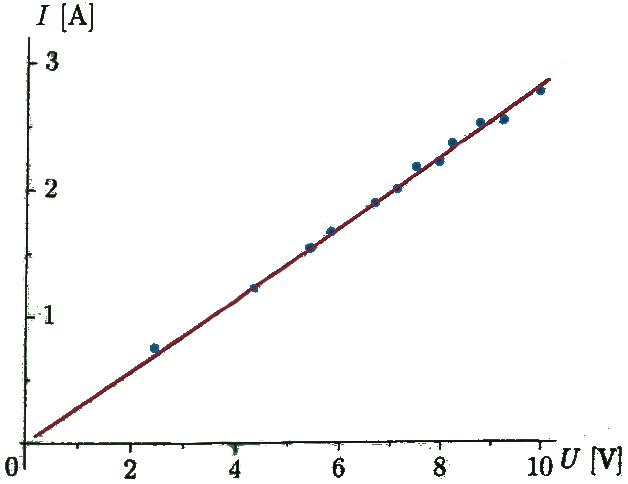
\includegraphics[width=0.8\linewidth]{mai_fig052.png}
  \captionof{figure}{Ověření Ohmová zákona lineární regresí.
  \cite[s.~263]{Musilova2009MA1}
  \label{mai:fig052}}
  \par}
  Pro odpor vychází \(R\doteq\SI{3.52}{\ohm}\). Součet čtverců odchylek přímky se směrnicí \(i/R
  = (1/\num{3.52})\Omega^{-1}\) od souboru bodů grafu je
  \begin{equation*}
    D(R) = \sum_{i=1}^{n}(U_i - R\cdot I_i)^2 \doteq\num{0.01},
  \end{equation*}
  \(\sigma(R) = \sqrt{D(R)/(n-1)}\doteq\sqrt{(\num{0.11}/11)}\doteq\num{0.03}\).  Graf přímky \(U
  = R\cdot I = \num{3.52}\cdot I\) proložené body je na obrázku \ref{mai:fig052}.
\end{mathexam}
      %---------------------------------------------------------------
      
      Popsaný způsob nalezení hodnoty elektrického odporu vodiče se nazývá\textbf{ metodou 
      nejmenších čtverců} (minimalizuje součet čtverců odchylek prokládané závislosti od souboru 
      naměřených bodů), v případě použití lineárního modelu, jako tomu bylo u Ohmová zákona, pak 
      jde o \textbf{lineární regresi}
      
      Obdobně se postupuje, je-li některá z měřených veličin lineární funkcí veličin jiných s 
      neznámými koeficienty lineární kombinace. Nechť
      \begin{equation*}
        Z = f(X_1, X_2, \ldots, X_K) = A_1X_1 + A_2X_2 + \cdots + A_KX_K.
      \end{equation*}
      Předpokládejme, že veličiny \(X_1, X_2, \ldots, X_K\) a \(Z\) měříme \(n\)-krát a naměříme 
      hodnoty
      \begin{equation*}
        X_j = \lbrace x_{j1}, \ldots x_{jn} \rbrace, \qquad 1 \leq j \leq K, \qquad 
        Z = \lbrace z_{1}, \ldots z_{n} \rbrace
      \end{equation*}
      Součet čtverců odchylek teoretické závislosti od naměřených bodů je
      \begin{equation*}
        D(Z) = \sum_{i=1}^{n}\left(z_i - \sum_{j=1}^{K}A_jx_{ji}\right)^2.
      \end{equation*}
      Nutnou podmínkou pro minimum tohoto výrazu jakožto funkce proměnných \(A_x, A_2, \ldots, A_K\)
      je platnost souboru rovnic
      \begin{equation*}
        \pder{D(Z)}{A_p} = 0 \Rightarrow 
        \sum_{i=1}^{n}2\left(z_i - \sum_{j=1}^{K}A_jx_{ji}\right)\cdot x_{pi} = 0
      \end{equation*}
      pro \(1 \leq i \leq n, 1 \leq j \leq K\). Tyto podmínky představují nehomogenní soustavu 
      \(K\) rovnic pro \(K\) neznámých \(( A_1, A_2, \ldots, A_K)\). Rozšířená matice soustavy je
      \begin{equation*}
        \overline{B} = (A|B) = 
          \left(
            \begin{array}{cccc|c}
              \sum_{i=1}^{n}x_{1i}x_{1i} & \sum_{i=1}^{n}x_{1i}x_{2i} & \cdots & 
              \sum_{i=1}^{n}x_{1i}x_{Ki} & \sum_{i=1}^{n}z_{i}x_{1i}                    \\
              \sum_{i=1}^{n}x_{1i}x_{1i} & \sum_{i=1}^{n}x_{2i}x_{2i} & \cdots & 
              \sum_{i=1}^{n}x_{2i}x_{Ki} & \sum_{i=1}^{n}z_{i}x_{2i}                    \\
                        \cdots           & \cdots & \cdots & \cdots   & \cdots          \\
              \sum_{i=1}^{n}x_{Ki}x_{1i} & \sum_{i=1}^{n}x_{Ki}x_{2i} & \cdots & 
              \sum_{i=1}^{n}x_{Ki}x_{Ki} & \sum_{i=1}^{n}z_{i}x_{Ki}                    \\
            \end{array}
          \right),
      \end{equation*}
      \begin{equation*}
        \sigma(z) = \sqrt{\dfrac{D(z)}{n - K}}.
      \end{equation*}
      V dalších kapitolách věnovaných lineární algebře se k tomuto problému znovu vrátíme a 
      ukážeme, že jej lze elegantně řešit také jako úlohu algebraickou, konkrétně úlohu o 
      ortogonální projekci vektorů na podprostory.
      
%} %tikzset
%---------------------------------------------------------------------------------------------------
\printbibliography[heading=subbibliography]
\addcontentsline{toc}{section}{Seznam literatury}
  % % !TeX spellcheck = cs_CZ
%{\tikzset{external/prefix={tikz/MAI/}}
% \tikzset{external/figure name/.add={ch05_}{}}
%---------------------------------------------------------------------------------------------------
% file: Differential_Calculus_applications.tex
%---------------------------------------------------------------------------------------------------
\setchaptertoc
\chapter{Aplikace diferenciálního počtu}\label{mai:IchapVI}

%================Kapitola: Analýza průběhu funkce ==================================================
\section{Analýza průběhu funkce}\label{mai:IchapVIsecI}
  Diferenciální počet má rozsáhlou oblast užití. V této kapitole ukážeme použití výsledků
  předchozích kapitol k vyšetřování průběhu funkce a vlastnosti rovinných křivek. Pomocí derivace
  můžeme studovat vlastnosti funkce, které usnadní vyšetřování jejího průběhu. 

  Jednou z důležitých vlastností funkce je její \uv{monotonie}, kterou jsme definovali již v odst.
  \ref{mai:IchapIIIsecIssecIII} kap. \ref{mai:IchapIII}. Proto je při vyšetřování průběhu
  funkce důležité určit množiny (často jsou to intervaly), na nichž je funkce monotónní, jinak
  řečeno, najít \uv{intervaly monotonie funkce} (viz
  \cite[s.~208]{Brabec1989}). 
    \begin{enumerate}[noitemsep]
      \item Zjistíme \textbf{definiční obor funkce}, vyjádříme jej v intervalech a z nich poznáme,
        kde je funkce \textbf{spojitá}. Funkce je spojitá v $(a,b)$ pro každý bod tohoto intervalu,
        když $\abs{f(x)-f(c)}<\varepsilon$, kde $\varepsilon>0$ je libovolně zvolené číslo, a pro
        všechna $x$ z okolí bodu $c$ je $\abs{x-c}<\delta$, kde $\delta>0$ je na $\varepsilon$
        nezávislé.
      \item Určíme, je-li funkce \textbf{lichá} $f(-x)=-f(x)$ nebo \textbf{sudá} $f(-x)=f(x)$. Je-li
        funkce lichá, je souměrná podle středu souměrnosti (obyčejně to bývá počátek souřadnic
        $xy$), je-li sudá, je souměrná podle osy $y$.
      \item Určíme \emph{průsečíky křivky s osami pravoúhlých souřadnic}. Body, ve kte\-rých křivka
        protíná osu $x$ spolu s body, ve kte\-rých není křivka spojitá, rozlišují intervaly, v nichž
        je graf křivky nad osou $x$ od intervalů, ve kterých je graf křivky pod osou $x$.
      \item V krajních bodech definičních intervalů, ve kterých je funkce spojitá, stano\-víme
      \emph{limity funkce} a dále $$\lim_{x \to \pm \infty}f(x).$$
      \item Vypočítáme $f'(x)$ a $f''(x)$, abychom zjistily, kde je funkce \emph{rostoucí}     
        $f'(x)>0$, \emph{klesající} $f'(x)<0$ a kde jsou \emph{lokální extrémy}. Dostaneme-li
        dosazením kořenů rovnice $f'(x)=0$ do $f''(x)$ hodnotu $f''(x)>0$, má funkce lokální
        minimum, při $f''(x)<0$ má funkce lokální maximum. V intervalech, kde $f''(x)>0$, je křivka
        \textbf{konvexní (vypuklá)}, kde $f''(x)<0$, je křivka \textbf{konkávní (vydutá)}. Body, v
        nichž $f''(x)$ mění znaménko, jsou \textbf{inflexní body}. Najdeme je tak, že stanovíme
        hodnoty $x$, pro které je $f''(x)=0$ nebo neexistuje. Číslo $c$ je inflexní bod, když
        existuje takové okolí bodu $c$, že pro $x>c$ je oblouk křivky konvexní a pro $x<c$ konkávní.
        Je nutné si uvědomit, že když má $f'(x)$ konečnou derivaci, je inflexní bod $c$ taky nulovým
        bodem druhé derivace čili kořenem rovnice $f''(x)=0$. Obrácená věta neplatí, tj. z
        $f''(x)=0$ nevyplývá, že v bodě $c$ má $f'(x)$ extrém a že bod $c$ je inflexním bodem.
      \item \textbf{Asymptota} je tečna křivky $f(x)$, jejíž bod dotyku je v nekonečnu. Platí-li  
        $$\lim_{x \to a}f(x) =  \pm\infty,$$ je přímka $x=a$ její asymptotou. Jinak asymptoty mají
        rovnici $y=kx+q$, kde $x$ a $y$ jsou souřadnice bodů na asymptotách. Existují-li konečné
        limity $$\lim_{x \to \pm\infty}\frac{f(x)}{x}=k$$  a $$\lim_{x \to \pm\infty}[f(x)-kx] =q$$
        pak je asymptotou přímka $y=kx+q$. Můžeme-li rovnici křivky rozložit (tj. rozložit její
        pravou stranu, oby\-čejně dělením čitatele jmenovatelem, má-li tvar zlomku) na dvě části, z
        nichž jedna má tvar $kx+q$ a druhá zbytek $\varphi(x)$, tj. $f(x)=kx+q+\varphi(x)$ a
        $\varphi(x)_{x\rightarrow \pm\infty}\rightarrow 0$, je přímka $y=kx+q$ asymptotou.
      \item Zpřesnění grafu křivky provedeme sestavením tabulky souřadnic dalších bodů křivky, tj.
        ke zvoleným hodnotám $x$ (z definičního oboru funkce) vypočítáme hodnoty $y$. Do dalších
        řádků tabulky zapíšeme hodnoty  $f'(x)$ a $f''(x)$, ve kterých intervalech je funkce
        \emph{rostoucí}, ve kterých \emph{klesá}, kde je \emph{vypuklá}, kde je \emph{dutá}, kde
        jsou \emph{lokální extrémy}, \emph{inflexní body} apod., případně sestavíme dílčí tabulky
        pro jednotlivé \emph{charakteristické vlastnosti} vyšetřované funkce.
    \end{enumerate}
    %-------------------- EXAM001 --------------------------------------
    % !TeX spellcheck = cs_CZ
\begin{mathexam}{Vyšetřete průběh funkce \(f(x):y=\frac{1+x^2}{1-x^2}\)}{exam003}
  \begin{enumerate}[noitemsep]
    \item Definiční obor $D_f=\realset-\{±1\}=(-\infty,-1)\cup(-1,1)\cup(1,+\infty)$
    \item Funkce je sudá $$f(-x)=f(x): \frac{1+x^2}{1-x^2}=\frac{1+(-x)^2}{1-(-x)^2}.$$ Funkce není
        periodická.
    \item Stanovíme funkční hodnoty v krajních bodech definičního obor $1, -1$ a v nevlastních
        bodech $-\infty,+\infty$.Protože je funkce \textbf{sudá}, omezíme se jen na vyšetřování
        nezáporné části. Nejprve vlastnosti funkce v okolí bodu $1$. Ten nepatří do $D_f$ a proto
        určíme limity funkce v pravém a levém okolí tohoto bodu. $$\lim_{x\to
        1_{-}}=\frac{1+x^2}{1-x^2}.$$ Pro výpočet limity použijeme substituci $y=1-x^2$: 
        $$\lim_{y\to0+}\frac{2-y}{y}=+\infty$$ \footnote{$\lim_{x\to0_+}\frac{1}{x}=\infty$} proto
        
        $$\lim_{x\to1_{-}}\frac{1+x^2}{1-x^2}=+\infty.$$ Obdobně dojdeme k
        $$\lim_{x\to1_+}\frac{1+x^2}{1-x^2}=-\infty.$$ A konečně v nevlastních bodech $±\infty$ je
        limita $$\lim_{x\to±\infty}\frac{1+x^2}{1-x^2} = \lim_{x\to\pm\infty}\frac{1}{1-x^2} +
        \lim_{x\to\pm\infty}\frac{x^2}{1-x^2}=0-1=-1.$$ Výpočtem limit jsme zároveň určili dva
        absolutní (globální) extrémy a jeden lokální:
        \begin{itemize}
          \item v intervalu $(-1,1)$ má funkce maximum $\infty$ a minimum $1$,
          \item v intervalech $(-1,1)\cup(1,+\infty)$ má funkce minimum $-\infty$ a maximum $-1$.
        \end{itemize}
    \item Nyní vyšetříme zda, případně kolik a jaké, má funkce $f(x)$ průsečíky s osami souřadnic. S
        osou $x$ nemá funkce žádné průsečíky, protože pro $y=0$ není definována
        $H_f=\realset-\{-1,1\rangle$. Pro $x=0$ je $y=\frac{1+0^2}{1-0^2}=1$, proto má $f(x)$ právě
        jeden průsečík s osou $y$ a to $[0,1]$.
    \item Zatím jsme zjistili, že naše funkce není definována v bodech $1$ a $-1$ a proto není
        spojitá v  $\realset$. Nevíme však, jaký je její průběh v jednotlivých intervalech
        definičního oboru.  Abychom získali názornější představu o průběhu funkce, zjistíme má-li
        derivaci.
        \begin{align*}
          y' &= \frac{(1+x^2)'(1-x^2 )-(1+x^2)(1-x^2 )'}{(1-x^2)^2} \\
          y' &= \frac{2x(1-x^2 )-(1+x^2 )(-2x)}{(1-x^2 )^2}         \\
          y' &= \frac{4x}{(1-x^2 )^2}
        \end{align*}
        Protože má vlastní derivaci\footnote{$f(x)$ je spojitá v intervalech $(-\infty,-1),
        (-1,1),(1,\infty)$  věta s spojité funkci}, můžeme určit její vlastnosti v intervalech
        $\langle0,1)$ a $(1,\infty)$. V těchto intervalech je $y'>0$ a proto jde o funkci ryze
        monotónní, rostoucí \footnote{Plyne z věty o postačujících podmínkách ryzí monotónnosti
        funkce na intervalu} v daných intervalech \footnote{V intervalech
        $(-\infty,-1),(-1,0\rangle$ je funkce klesající.}. Výpočtem zjistíme druhou derivaci funkce.
        Ta nám pomůže určit další extrém v intervalu $\langle0,1)$ a zároveň vyšetřit
        \textbf{konkávnost} a \textbf{konvexnost}.
        \begin{align*}
          y'' &= \frac{(4x)' (1-x^2 )^2-(4x)(1-2x^2+x^4 )'}{(1-x^2 )^4}  \\
          y'' &= \frac{4(1-2x^2+x^4 )-4x(-4x+4x^3 )}{(1-x^2 )^4}         \\
          y'' &= \frac{4(1-x^2 )(3x^2+1)}{(1-x^2 )^4}                    \\
          y'' &= \frac{4(3x^2+1)}{(1-x^2 )^3}
        \end{align*}
        Abychom mohli určit lokální extrém funkce $f(x)$ v intervalu $\langle0,1)$, pomocí druhé
        derivace, musíme najít kořeny rovnice $f' (x)=0$. V našem případě
        $$y'=\frac{4x}{(1-x^2)^2}\Rightarrow\frac{4x}{(1-x^2)^2}=0\rightarrow x_0=0,$$ tento kořen
        \footnote{stacionární bod}  pak dosadíme do druhé derivace, tj. 
        $$y''(0)=\frac{4(3\cdot0^2+1)}{(1-0^2 )^3}=4,$$ protože je $f''(x)>0$, má v bodě $x_0$
        lokální minimum. Můžeme rovněž konstatovat, že funkce nemá inflexní body \footnote{Pro
        existenci inflexního bodu je nutné splnění jedné z podmínek a to buď $f''(x_0)=0$, nebo
        $f''(x_0)$ neexistuje.}. Konkávnost a konvexnost funkce v intervalech $\langle0,1)$ a
        $(1,\infty)$ vyšetříme pomocí vlastností druhé derivace funkce. Tedy
        \begin{itemize}
          \item $\langle0,1): y''=\frac{4(3x^2+1)}{(1-x^2 )^3} >0 \Rightarrow$ funkce je v tomto
                intervalu \textbf{konvexní},
          \item $(1,\infty): y''=\frac{4(3x^2+1)}{(1-x^2 )^3} <0 \Rightarrow$ funkce je v tomto
                intervalu \textbf{konkáv\-ní}.
        \end{itemize}
    \item Z předchozích výpočtů plyne, že křivka má asymptoty $y=-1,x=\pm1$.
  \end{enumerate}
  {\centering \captionsetup{type=figure}          % %\ref{MAI:fig_028}
    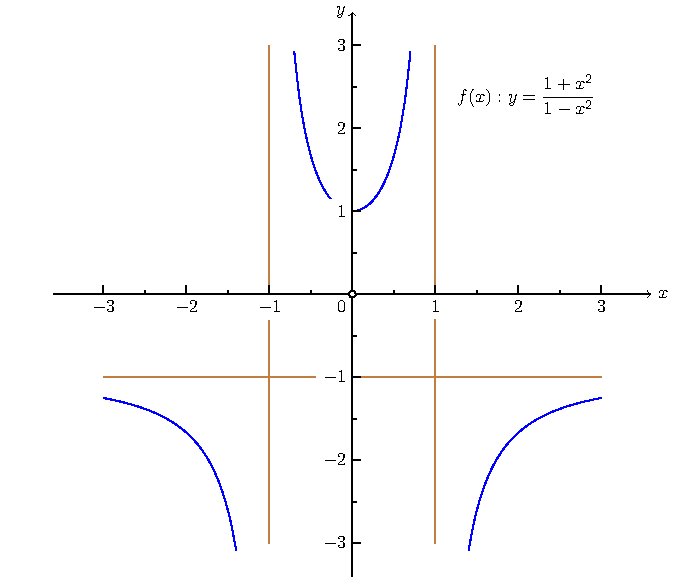
\includegraphics[width=1\linewidth]{mai_fig028.pdf}
    \captionof{figure}{Graf funkce $f(x):y=\dfrac{1+x^2}{1-x^2}$}
    \label{MAI:fig_028}
  \par}
\end{mathexam}  
    %-------------------------------------------------------------------

%================Kapitola: Aplikace diferenciálního počtu =========================================
\section{Fyzikální a jiné aplikace derivace}\label{mai:IchapVIsecII}
    V předcházející kapitole \ref{mai:IchapVIsecI} jsou uvedeny jednoduché příklady na užití první a
    druhé derivace. V této kapitole jsou soustředěny slovní úlohy na maxima a minima z různých
    oborů.
    %--------------------------------------------------------------
    % !TeX spellcheck = cs_CZ
\begin{mathexam}{Je dán trojúhelník s vrcholy \(A[0, 0]\), \(B[4, 0]\), \(C[1, 3]\). Mezi všemi
  obdélníky vepsanými danému trojúhelníku, se stranou („základnou“) \(z\) ve straně \(c\) (označení
  viz obr. \ref{mai:fig062}), máme najít ten, který má maximální obsah.}{exam092}

  {\centering
    \captionsetup{type=figure}
    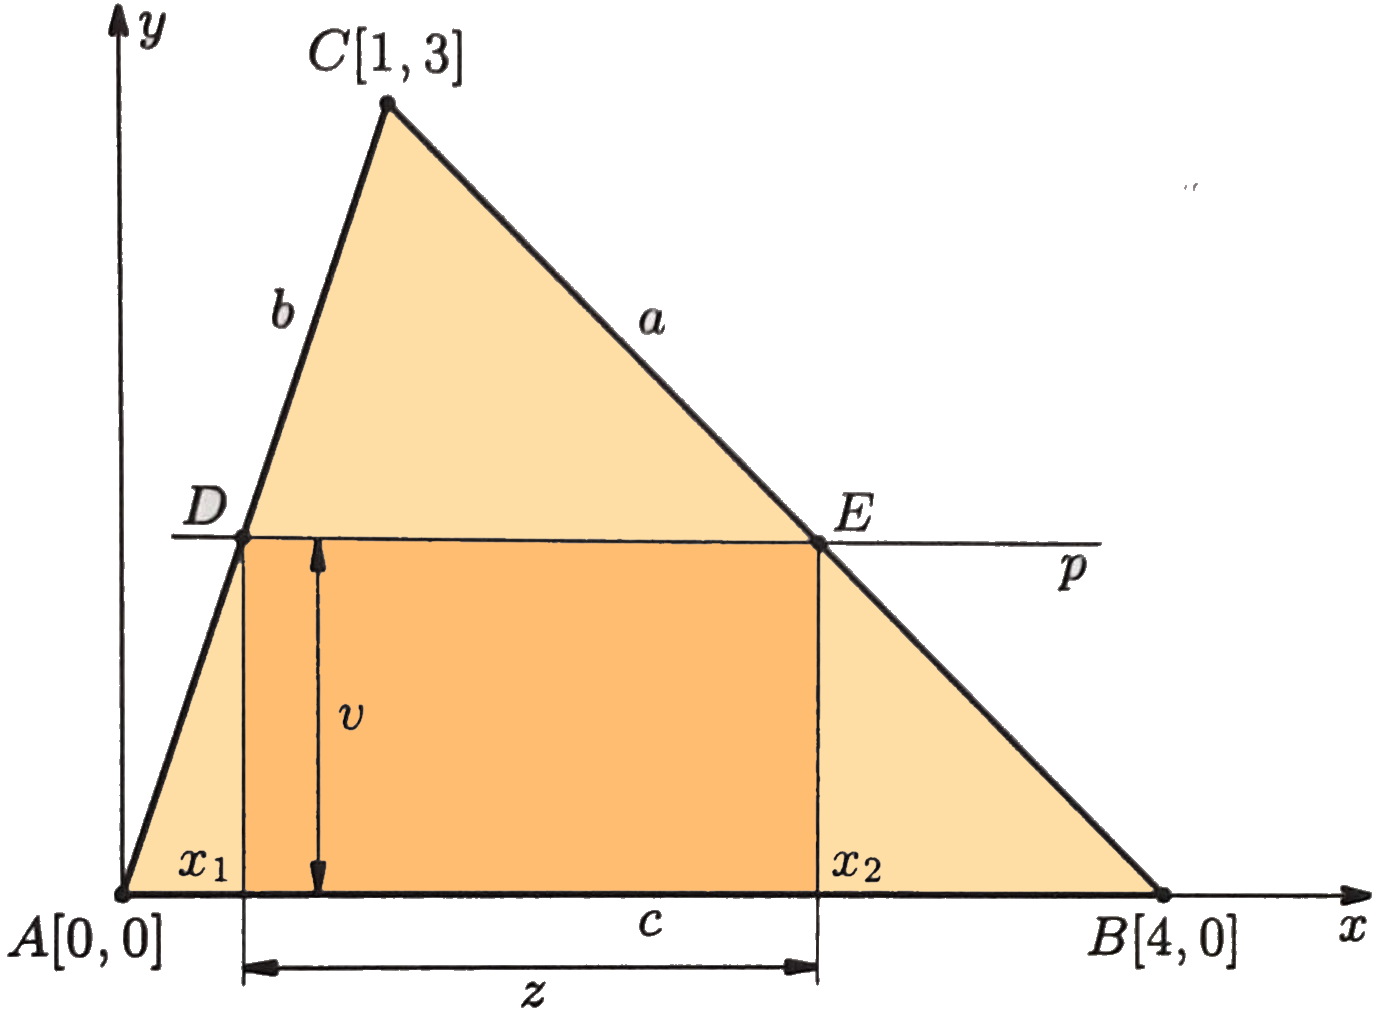
\includegraphics[width=1\linewidth]{mai_fig062.png} 
    \captionof{figure}{K příkladu \ref{mai:exam092}. Kredit: \cite[s.~46]{rektorys2011}}
    \label{mai:fig062}
  \par}
  
  Napišme nejprve rovnice stran \(a\), \(b\). Strana \(b\) (přesněji: přímka obsahující stranu
  \(b\)) má zřejmě rovnici
  \begin{equation*}
    y = 3x
  \end{equation*}
  Přímka, v níž leží strana \(a\), má směrnici
  \begin{equation*}
    k = \dfrac{3-0}{1-4} = -1,
  \end{equation*}
  a tedy podle rovnice \(y-y_0 = k(x-x_0)\) dostáváme 
  \begin{equation*}
    y - 0 = -1\cdot(x - 4) \quad\Rightarrow\quad y = -x + 4.  
  \end{equation*}
  Pro obsah \(S\) vepsaného obdélníka platí podle označení v obr. \ref{mai:fig062} 
  \begin{equation*}
    S = zv.
  \end{equation*}
  Za proměnnou zde bude výhodné volit „výšku“ \(v\). „Základnu“ \(z\) pak vypočteme (viz obr.
  \ref{mai:fig062}) jako rozdíl
  \begin{equation}\label{mai:eq087}
    z = x_2 - x_1,
  \end{equation}
  kde \(x_1\), resp. \(x_2\) je souřadnice \(x\) průsečíku přímky \(y = v\) (přímka \(p\) na obr.
  \ref{mai:fig062}) se stranou \(b\), resp. \(a\). Rovnice těchto stran jsou dány vztahy \(y = 3x\)
  a \(y = -x + 4\). Dosadíme-li podle \(y = v\rightarrow\)  \(v\) za \(y\) do těchto rovnic,
  dostaneme právě \(x_1\) a \(x_2\). Bude
  \begin{equation*}
    v = 3x_1, \qquad v = -x_2 + 4,
  \end{equation*}
  odkud (při zvoleném \(v\)) plyne
  \begin{equation*}
    x_1 = \dfrac{v}{3}, \qquad  x_2 = 4 - v 
  \end{equation*}
  a podle \ref{mai:eq087}
  \begin{equation*}
    z = x_2 - x_1 =  4 - \dfrac{4}{3}v
  \end{equation*}
  a konečně pro obsah vepsaného obdélníku dostáváme jednoduchou rovnici
  \begin{equation}\label{mai:eq088}
    S = zv = \left(4 - \dfrac{4}{3}v\right)v = 4v - \dfrac{4}{3}v^2.
  \end{equation} 
  Tím je obsah \(S\) obdélníka daný jako funkce zvolené výšky \(v\). Zvolíme-li například \(v=1\),
  bude obsah \(S\) obdélníka z obr. \ref{mai:fig062} roven číslu \(4\cdot1 - \frac{4}{3}\cdot1^2\). 
  
  Budeme hledat (absolutní) maximum funkce (\ref{mai:eq088}) na intervalu \(\langle0,3\rangle\)
  (neboť nemůžeme zvolit \(v\) větší než 3). Ale pro \(v=0\) a \(v=3\) je \(S=0\) a všude jinde je
  \(S > 0\), takže budeme hledat lokální maximum funkce (\ref{mai:eq088}) na otevřeném intervalu
  \((0,3)\). Derivováním (\ref{mai:eq088}) podle proměnné \(v\) však máme
  \begin{equation*}
    S' = 4 - \dfrac{8}{3}v, \qquad S'' = -\dfrac{8}{3}.
  \end{equation*}
  Položíme-li nyní pravou stranu rovnu nule, dostaneme 
  \begin{equation*}
    4 - \dfrac{8}{3}v = 0 \quad\Rightarrow\quad v = \dfrac{12}{8} = \dfrac{3}{2}.
  \end{equation*}
  Přitom podle druhé derivace obsahu je všude, a tedy i v bodě \(\frac{3}{2}\), je
  \(S''=-\frac{8}{3}<0\) takže v bodě \(v = \frac{2}{3}\) je ostré lokální maximum. Zároveň pro
  \(v=\frac{3}{2}\) bude
  \begin{equation*}
    z = 4 - \dfrac{4}{3}\cdot\dfrac{3}{2} = 2.
  \end{equation*}
  Hledaný obdélník maximálního obsahu bude mít rozměry: \(z = 2\), \(v = \frac{3}{2}\), a tedy obsah
  \(S = 3\).    
\end{mathexam}
    %--------------------------------------------------------------

    %--------------------------------------------------------------
    % !TeX spellcheck = cs_CZ
\begin{mathexam}{Z břevna kruhového průřezu s poloměrem \(r = \protect\SI{20}{\protect\cm}\) máme
  vytesat trám, který bude mít průřez ve tvaru obdélníka se stranami \(z\) a \(v\) („základnou“ a
  „výškou“). Jak máme volit \(z\) a \(v\), aby trám měl maximální nosnost, víme-li, že jeho nosnost
  je úměrná první mocnibibeně \(z\) a druhé mocnině \(v\)?}{exam091}
   
  {\centering
    \captionsetup{type=figure}
    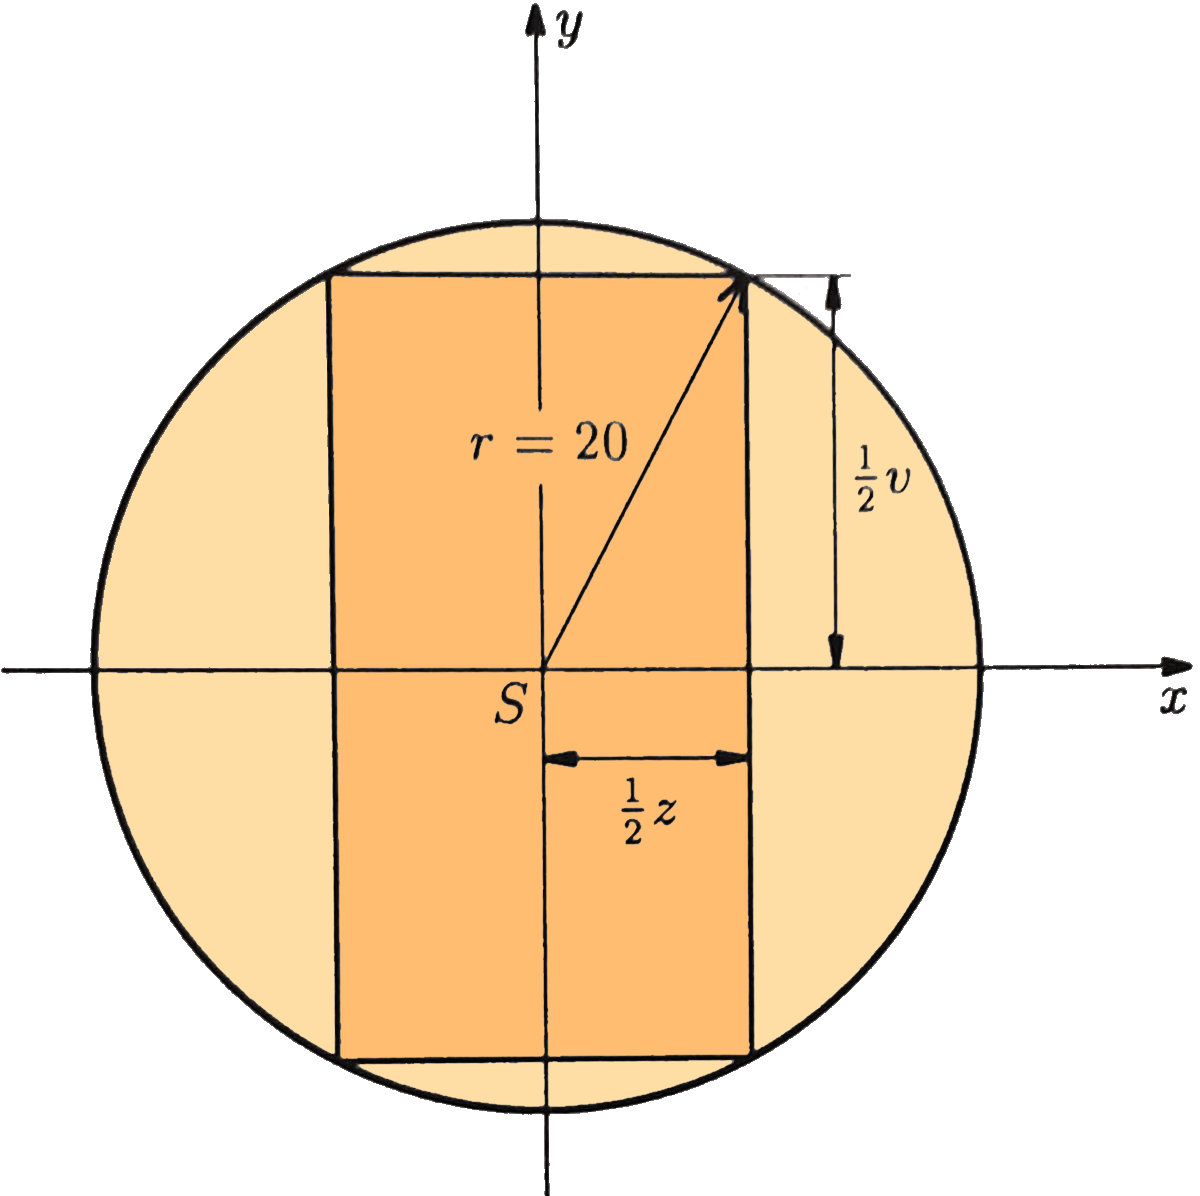
\includegraphics[width=1\linewidth]{mai_fig061.png} 
    \captionof{figure}{K příkladu \ref{mai:exam091}. Kredit: \cite[s.~47]{rektorys2011}}
    \label{mai:fig061}
  \par}
  
  Matematická formulace: Jaké rozměry má mít obdélník vepsaný do kružnice s poIoměrem \SI{20}{\cm},
  má-li být součin základny \(z\) a druhé mocniny výšky v maximální,
  \begin{equation*}
    y = z\cdot v^2 = ?
  \end{equation*}
  Zvolme za proměnnou z. Podle Pythagorovy věty platí (viz \ref{mai:fig061})
  \begin{equation*}
      r^2 = \left(\dfrac{z}{2}\right)^2 + \left(\dfrac{v}{2}\right)^2,
  \end{equation*}
  odkud 
  \begin{equation*}
      v^2 = 4r^2 - z^2.
  \end{equation*}
  Máme tedy najít maximum funkce
  \begin{equation}\label{mai:eq086}
      y = zv^2 = z(4r^2 - z^2) = 4r^2z - z^3,
  \end{equation}
  a to na intervalu \((0,40)\), neboť \(z\) nemůže být větší než \(2r = 40\). Ale funkce
  (\ref{mai:eq086}) je na tomto intervalu nezáporná a pro \(z = 0\) a \(z = 40\) je rovna nule
  (neboť pak \(4r^2 - z^2 = 0\). Hledáme tedy lokální maximum funkce (\ref{mai:eq086}) v otevřeném
  intervalu \(0,40)\). 

  Funkce (\ref{mai:eq086}) má všude první a druhou derivaci,
  \begin{equation*}
      y' = 4r^2 - 3z^2, \qquad\qquad y'' = -6z.
  \end{equation*}
  Může tedy předně nabývat v intervalu \((0, 40)\) lokálního extrému jen tam, kde je \(y'=0\), tj.
  kde
  \begin{equation*}
      4r^2 - 3z^2 = 0.
  \end{equation*}
  Odtud plyne, neboť má být \(z > 0\), že
  \begin{equation*}
      z = \sqrt{\dfrac{4r^2}{3}} = \dfrac{2}{\sqrt{3}}r = \dfrac{2\sqrt{3}}{3}r = 
          \dfrac{2\sqrt{3}}{3}20 \simeq \num{23.1}.
  \end{equation*}
  Pro \(v\) pak \(z\) dostaneme
  \begin{equation*}
      v = \sqrt{4r^2 - \dfrac{4}{3}r^2} = \sqrt{\frac{8}{3}\cdot20^2}\simeq\num{32.6}
  \end{equation*}
  V bodě \(z = \num{23.1}\) bude mít funkce (\ref{mai:eq086}) skutečně lokální maximum, a to ostré,
  neboť druhá derivace je v tomto bodě záporná.
\end{mathexam}
    %--------------------------------------------------------------

    %--------------------------------------------------------------
    % !TeX spellcheck = cs_CZ 
\begin{mathexam}{Světelný zdroj \(B\) (např. pouliční svítilna) má vzdálenost \qty{36}{\m} od
  světelného zdroje \(A\). Zdroj \(B\) má osmkrát větší intenzitu než zdroj \(A\). Který bod na
  spojnici obou zdrojů bude nejméně osvětlený? (Přitom intenzita osvětlení světelným zdrojem je
  přímo úměrná intenzitě zdroje a klesá s druhou mocninou vzdálenosti od uvažovaného
  zdroje.)}{exam093} 
  
  {\centering
    \captionsetup{type=figure}
    \luafigure[1]{mai_fig063.png} 
    \captionof{figure}{K příkladu \ref{mai:exam093}. Kredit: \cite[s.~48]{rektorys2011}}
    \label{mai:fig063}
  \par}      

  Matematická formulace: Označme \(a\) intenzitu zdroje \(A\). Pak intenzita zdrojo \(8\) je \(8a\).
  Označme dále \(x\) vzdálenost bodu \(P\) na spojnici bodů \(A\) a \(B\) meřenou od zdroje \(A\).
  Pak intenzita osvětlení v bodě \(P\) od zdroje \(A\) bude úměrná číslu \(\frac{a}{x^2}\) zdroje B
  číslu \(\frac{8a}{(36 - x)^2}\) (se stejnou konstantou úměrnosti). Máme tedy najít v intervalu
  \((0,36)\) takové \(x\), pro které bude součet obou intenzit minimalni, a tj.
  \begin{equation}\label{mai:eq089}
    y = \dfrac{a}{x^2} + \dfrac{8a}{(36 - x)^2} = \text{min}
  \end{equation}
  Ale funkce \ref{mai:eq089} má všude v otevřeném intervalu  \((0,36)\) první a druhou derivaci.
  Nastává chvíle si procvičit derivování podílu:
  \begin{gather*}
    \begin{align*} 
      \left(\dfrac{a}{x^2}\right)'          
        &= (ax^{-2})' = -\dfrac{2a}{x^3},   \\ 
      \left( \dfrac{8a}{(36 - x)^2}\right)' 
        &= \dfrac{(8a)'\cdot(36 - x)^2 - (8a)\cdot(36^2 - 72x + x^2)'}{(36 - x)^4} \\
        &= \dfrac{-8a(-72 + 2x)}{(36 - x)^4} 
         = +\dfrac{8a\cdot2\cdot\cancel{(36 - x)}}{(36 - x)^{\cancel{4}3}}
         =  \dfrac{16a}{(36 - x)^3}
    \end{align*}
  \end{gather*}
  (neboť \(8a = \text{konst}\), takže \((8a)' = 0\); k derivování funkce \(8a/(36 - x)^2\) jsme také
  mohli místo věty o derivování podílu použít větu o derivování složených funkcí a psát
  \begin{equation*}
    \dfrac{8a}{(36 - x)^2} = \dfrac{8a}{z}, \quad\text{kde}\quad z = 36 - x
  \end{equation*}  
  Tedy 
  \begin{align*}
    y'  &= -\dfrac{2a}{x^3} + \dfrac{16a}{(36 - x)^3} \\
    y'' &=  \dfrac{6a}{x^4} + \dfrac{48a}{(36 - x)^4}. 
  \end{align*}
  Jak víme, v bodě lokálního minima bude \(y' = 0\)
  \begin{equation}\label{mai:eq090}
    -\dfrac{2a}{x^3} + \dfrac{16a}{(36 - x)^3} = 0.
  \end{equation}
  Rovnici můžeme řešit tak, že zlomky na levé straně dáme na společného jmenovatele. (Zkuste to,
  nebude to hezká rovnice!) Ale má být \(x > 0\), \(36 - x > 0\), takže (\ref{mai:eq090}) můžeme
  zapsat ve tvaru
  \begin{align*}
    \dfrac{(36 - x)^3}{x^3} &= -\dfrac{16a}{2a} = 8 \qquad\text{takže}      \\
    \dfrac{36 - x}{x}       &= \sqrt[3]{8} \Rightarrow 36 - x = 2x.
  \end{align*}
  Zároveň \(y''>0\), takže v bodě \(x=12\) bude ostré lokální minimum. Nejméně osvětlený bod bude
  tedy ve vzdálenosti \qty{12}{\m} od zdroje \(A\).

  {\centering
  \captionsetup{type=figure}
  \luafigure[1]{mai_fig064.pdf} 
  \captionof{figure}{K příkladu \ref{mai:exam093}.}
  \label{mai:fig064}
  \par}   
\end{mathexam}
    %--------------------------------------------------------------

%} %tikzset
%---------------------------------------------------------------------------------------------------
  % \input{../src/MAI/chap/mai1ch04.tex}
  % !TeX spellcheck = cs_CZ
%---------------------------------------------------------------------------------------------------
% file: mai1ch07.tex
%---------------------------------------------------------------------------------------------------
%============================ Primitivní funkce ====================================================
\setchaptertoc
\chapter{Poznáváme funkci z její derivace - neurčitý integrál}
  %----------------------------Neurčitý integrál----------------------------------------------------
  \section{Motivace}
    Problém \emph{neurčitého integrálu}, neboli \textbf{primitivní funkce}, lze vyložit velmi 
    jednoduše: Máme podezření, že zadaná funkce \(f(x)\) vznikla derivováním jisté, zatím neznámé, 
    funkce \(F(x)\). Dokážeme ji najít? 
  
    K danému problému můžeme přistupovat také fyzikálně: Zavedením pojmu derivace funkce jsme 
    motivovali důležitým požadavkem definovat okamžitou rychlost pohybu bodu po přímce. Existuje 
    přirozeně i požadavek opačný, tj. nalézt zákon dráhy pohybu bodu po přímce, je-li dána jeho 
    okamžitá rychlost jako funkce času \cite[s.~253]{Brabec1989}. Vše si ukážeme na následujícím 
    příkladu:      
    %-------------------------------------
    % !TeX spellcheck = cs_CZ
%====================== Sbírka řešených příkladů ==================================================
\begin{mathexam}{Je dána okamžitá rychlost \(v\) pohybu bodu po přímce (ose) \(x\) rovnicí \(v(t) =
  2t + 1\), \(t\in\langle -\infty,+\infty \rangle\). Najděte zákon dráhy pohybu, je-li známo, že v
  čase \(t = 0\) měl bod polohu \(x = x_0\) \cite[p.~253]{Brabec1989}.}{exam117}

  Označíme-li \(x(t)\) polohu bodu v okamžiku \(t\), pak \(v(t) = \frac{dx}{dt}\). Hledáme tedy
  funkci \(x = x(t)\), pro níž platí \[\frac{dx}{dt} = 2t + 1 \qquad x(0) = x_0.\] Je ihned patrné,
  že první podmínce vyhovuje nekonečně mnoho funkcí
  \begin{equation}\label{MA:int_ex_09}
    x(t) = t^2 + t + c, 
  \end{equation}
  kde \(c\) je libovolná konstanta. Funkce, která splňuje i druhou podmínku (říkáme ji též počáteční
  podmínka), najdeme z rovnice \ref{MA:int_ex_09} dosazením dané podmínky \(t = 0\), \(x = x_0\).
  Dostaneme \(x_0 = c\). Dosazením do \ref{MA:int_ex_09} za \(c\) plyne hledaný zákon dráhy \(x(t) =
  t^2+t+x_0\).                 

  Jednoduchou zkouškou se přesvědčíme, že tato funkce splňuje obě dané podmínky a zároveň vidíme, že
  hledaná primitivní funkce daných vlastností je jediná.
\end{mathexam}
    %-------------------------------------
    Každé takové funkci, jejíž derivací je daná funkce, budeme říkat \emph{primitivní funkce} k 
    dané funkci. Na uvedeném příkladě je patrné, že k dané funkci může existovat nekonečně mnoho 
    primitivních funkcí. Množinu všech primitivních funkcí se často nazývá \textbf{neurčitým 
    integrálem}. Po tomto názorném uvedení do problému přejděme k přesné formulaci základních pojmů.
    
  \section{Definice primitivní funkce}  
    \begin{mdframed}[style=mdmathdef] 
      \begin{definition}\label{mai:def002}
        Funkci \(F(x): J\rightarrow \realset\), kde \(J\subset \realset\) je interval, nazveme
        \textbf{primitivní} funkcí k funkci \(f(x)\) na intervalu \(J\) právě když, pro všechna
        \(x\in J\) je \(F'(x) = f(x)\). 
        
        V případě uzavřeného intervalu \(J=[a,b]\) požadujeme ještě, aby obě jednostranné derivace
        splňovali \(F_+'(a)=f(a)\) a \(F_-'(b)=f(b)\). 
        
        Množina všech primitivních funkcí k funkci \(f(x)\) na \(J\) se nazývá \textbf{neurčitý
        integrál} z funkce \(f(x)\) a značí se \(\int f(x)\dd{x}\). Tedy
        \begin{gather}\label{mai:eq101}
          \int f(x)\dd{x} = \{F(x): \text{\(F(x)\) je primitivní funkcí k \(f(x)\) na \(J\)}\}
        \end{gather}
      \end{definition}
    \end{mdframed}
    %-------------------------------------
    % !TeX spellcheck = cs_CZ
%====================== Sbírka řešených příkladů ==================================================
\begin{mdframed}[style=mdexam]
  \begin{example}\label{mai:exam118}
    K funkci $\sin x$ je primitivní funkcí na libovolném intervalu $J\subset(-\infty,+\infty)$ 
    funkce $-\cos x$, protože $(-\cos x)' = \sin x$. Ale též funkce $3-\cos x$ je primitivní 
    funkcí k funkci $\sin x$, protože $(3 - \cos x)' = \sin x$ pro všechna $x\in(-\infty, 
    \infty)$.
  \end{example}
\end{mdframed}
    %-------------------------------------
    
    Z uvedených příkladů je vidět, že rozdíl dvou primitivních funkcí k téže funkci je konstanta. To
    není náhoda, jak potvrzuje následující věta:

    \begin{mdframed}[style=mdmathlemma] 
      \begin{lemma}\label{mai:lemma008}(Věta o rozdílu dvou primitivních funkcí)
        \begin{enumerate}[noitemsep]
          \item Je-li funkce $F$ primitivní funkcí k funkci \(f\) na intervalu \(J\) a \(c\) reálná  
                konstanta, pak i funkce $G = F + c$ je primitivní funkcí k funkci \(f\) na intervalu 
                \(J\).
          \item Jsou-li funkce $F$ a $G$ primitivní funkce k funkci \(f\) na intervalu \(J\), pak 
          funkce
                $F-G$ je na intervalu \(J\) konstantní.
        \end{enumerate} 
        \begin{proof}
          Tvrzení a) plyne z definice protože $G'(x) = [F(x) + c] = F'(x) = f(x)$ pro všechna $x\in
          J$. Tvrzení b) je důsledkem věty \ref{MA1:lem_diff01}.
        \end{proof}
      \end{lemma}
    \end{mdframed}

    \subsection{Poznámky k definici}  
      Z definice \ref{mai:def002} vyplývá, že primitivní funkce je spojitou funkcí, neboť má
      derivaci a věta \ref{mai:lemma008} nám říká, že pokud k dané funkci existuje funkce
      primitivní, existuje jich nekonečně mnoho. Je-li např. \(F\) primitivn9 funkce k funkci \(f\)
      na intervalu \(J\), pak množina všech primitivních funkcí je množina \(\{F + c;
      c\in\realset\}\). Tuto množinu označujeme symbolem \(\int f(x)\dd{x}\) a čteme \uv{integrál
      \(f(x)\dd{x})\)} Symbolu \(\int f(x)\dd{x}\) říkáme \textbf{neurčitý integrál}. Zpravidla
      píšeme
      \begin{mdframed}[style=mdmathlemma]  
        \begin{equation}\label{mai:eq102}
          \int f(x)\dd{x} = F(x) + c
        \end{equation}
      \end{mdframed}
      nebo jen \(\int f(x)\dd{x} = F(x)\) (tj. aditivní konstantu vynecháváme) a máme tím na mysli
      že \(F(x) \in \int f(x)\dd{x}\). Rovnost \ref{mai:eq102} je tedy rovnost mezi množinami,
      nikoliv rovnost funkcí. 
    
    \subsection{Některé vlastnosti integrálů}  
      Platnost několika následujících vztahů lze prověřit přímo užitím definic derivace a neurčitého
      integrálu. Tyto vztahy jsou při výpočtech často používány. Nejprve však uvedeme základní
      pravidla pro primitivní funkce, která plynou z pravidel pro derivování:
      \begin{subequations}
        \begin{flalign}
          \int\dd{f(x)} &= f(x) + c,                                          &\label{mai:eq134} \\
          \dxd\left[\int f(x)\dd{x}\right] &= f(x)\dd{x},                     &\label{mai:eq135} \\
          \int[f(x)\pm g(x)]\dd{x}&= \int f(x)\dd{x} + \int g(x)\dd{x},       &\label{mai:eq103} \\
          \int kf(x)\dd{x}      &=k\int f(x)\dd{x},\quad\text{\(k=\) konst.}, &\label{mai:eq104} \\
          \left[\int f(x)\dd{x}\right]' &= f(x),                              &\label{mai:eq136}
        \end{flalign}
      \end{subequations}
  
  \section{Tabulka neurčitých integrálů}\label{MA:chap_tabINT}
    Jak ale primitivní funkce hledat? V jednoduchých příkladech poslouží tabulka derivací, již čteme
    „zprava doleva“. (Je dobré si ji uložit do paměti.) Tabulka však pokryje jen velmi málo případů,
    pouze elementární funkce. Je tedy třeba najít metody, jak při hledání primitivních funkcí
    postupovat.

    Uveďme nyní některé základní integrály. Poznamenejme, že touto tabulkou nejsou zdaleka vyčerpány
    všechny funkce, ke kterým umíme primitivní funkce najít. Existují celé knihy obsahující tabulky
    integrálů a programy výrazně ulehčující hledání primitivních funkcí. Literatura:
    \cite{Rektorys1963}, \cite{Brabec1989}, \cite{diblik2002}. 

    Pokud není nic uvedeno, platí vzorce pro všechna \(x\) a pro všechny hodnoty uvedených konstant.
    Místo platí pro \(x\) z intervalu \((-\infty,0),(0,+\infty)\) píšeme stručně \(x\neq0\) apod.
    Obory platnosti uvádíme jen tam, kde nejsou evidentní.  

    \begin{flalign}
      \midrule
      & \int 0\dd{x} = c                                        &      \label{mai:eq105}     \\
      & \int a\dd{x} = ax+c                                     &      \label{mai:eq106}     \\
      & \int x^n\dd{x} = \frac{x^{n+1}}{n+1}+c,                 &      \label{mai:eq107}     \\              
        \shortintertext{\hspace{2em} kde \(\begin{cases}
          \forall x\in\realset,\,n\in\naturalset, n>0,         \\
          \forall x\in\realset-\{0\},\,n\in\naturalset, n<-1,  \\
          \forall x>0,\,n\in\realset\,\,n\neq-1
        \end{cases}\)}                                          
      & \int\frac{1}{x}\dd{x} = 
            \ln\abs{x}+c \hspace{1ex}\forall x\neq0            &       \label{mai:eq108}    \\
      & \int e^x \dd{x}       = e^x+c                          &       \label{mai:eq109}    \\
      & \int\ln x\dd{x}       = 
          x\ln x - x + c \hspace{1ex}\forall x>0               &       \label{mai:eq110}    \\
      & \int a^x \dd{x}     =
        \frac{a^x}{\ln a}+c 
        \hspace{1ex}\forall a>0,\,a\neq1                       &       \label{mai:eq111}    \\
      & \int \sin x \dd{x}  = -\cos x                          &       \label{mai:eq112}    \\
      & \int \cos x \dd{x}  =  \sin x                          &       \label{mai:eq113}    \\
      & \int\frac{1}{\cos^2x}\dd{x} =  \tan x + c              &       \label{mai:eq114}    \\
        \shortintertext{\(\hspace{2em}\forall x\neq\frac{1}{2}\pi+k\pi,\,k\in\naturalset\)}\nonumber\\       
      & \int\frac{1}{\sin^2x}\dd{x}     =  -\cotg x+c         &        \label{mai:eq115}    \\
        \shortintertext{\(\hspace{1em}\forall x\neq k\pi,\,k\in\naturalset\)}
      & \int\frac{1}{\sqrt{1-x^2}}\dd{x} =
          \begin{cases}
            +\arcsin x + c         \\
            -\arccos x + c
          \end{cases}                                          &      \label{mai:eq116}    \\
        \shortintertext{\(\hspace{2em}\forall x\in(-1,1) \)}  
    & \int\sinh x\dd{x} = \cosh x + c                         &       \label{mai:eq117}    \\
    & \int\dfrac{1}{\sinh x}\dd{x} = -\cotgh x + c            &       \label{mai:eq118}    \\
    & \int\cosh x\dd{x} = \sinh x + c                         &       \label{mai:eq119}    \\
    & \int\dfrac{1}{\cosh x}\dd{x} = -\tanh x + c             &       \label{mai:eq120}    \\
    & \int\frac{1}{1+x^2}\dd{x} = \arctan x + c               &       \label{mai:eq121}    \\
    & \int\frac{1}{\sqrt{x^2 + 1}}\dd{x} =
        \begin{cases}
            \ln(x + \sqrt{x^2+1}) + c         \\
            \arcsinh x            + c 
        \end{cases}                                           &       \label{mai:eq122}    \\ 
    & \int \frac{1}{\sqrt{x^2 - 1}}\dd{x} =
        \begin{cases}
            \ln(x + \sqrt{x^2-1}) + c         \\
            \arccosh x            + c  
        \end{cases}                                           &       \label{mai:eq123}    \\   
      \shortintertext{\hspace{2em}\(x\in(1,+\infty)\)}  
    & \int\frac{1}{\sqrt{x^2+a^2}}\dd{x} 
        = \begin{cases}
              \arcsinh\frac{x}{a}   + c  \\ 
              \ln(x+\sqrt{x^2+a^2}) + c     
          \end{cases}                                          &      \label{mai:eq124}    \\
    & \int \frac{1}{\sqrt{x^2-a^2}}\dd{x} 
        = \begin{cases}
              \arccosh\frac{x}{a}   + c   \\
              \ln(x+\sqrt{x^2-a^2}) + c
          \end{cases}                                          &      \label{mai:eq125}    \\
    & \int\tan x \dd{x}   = \ln\abs{\sec x} + c                &      \label{mai:eq126}    \\
    & \int\sec x \dd{x}   = \ln\abs{\sec x + \tan x} + c       &      \label{mai:eq127}    \\
    & \int\sec^2 x \dd{x} = \tan x + c                         &      \label{mai:eq128}    \\
    & \int\sec x\tan x \dd{x} = \sec x + c                     &      \label{mai:eq129}    \\
    & \int\frac{a}{a^2+x^2}\dd{x} = \tan^{-1}\frac{x}{a} + c   &      \label{mai:eq130}    \\
    & \int\frac{a}{a^2-x^2}\dd{x} = 
      \frac{1}{2}\ln\left\lvert\frac{x+a}{x-a}\right\rvert     &      \label{mai:eq131}    \\
    & \int\frac{1}{\sqrt{a^2-x^2}} \dd{x} = 
      \sin^{-1} \frac{x}{a}                                    &      \label{mai:eq132}    \\
    & \int\frac{a}{x\sqrt{x^2-a^2}}\dd{x} = 
      \sec^{-1} \frac{x}{a}                                    &      \label{mai:eq133}    \\
      \midrule  
    \end{flalign}

    \begin{mdframed}[style=mdmathlemma]  
      \(\argsinh x\), \(\argcosh x\), \(\argtanh x\), \(\argcoth x\) jsou funkce inverzní k
      hyperbolickým funkcím. Značení těchto funkcí není jednotné. Správné zkratky jsou ty, které
      specifikuje norma \texttt{ISO 80000-2}. Skládají se z \uv{ar} následovaných zkratkou
      odpovídající hyperbolické funkce (např. arsinh, arcosh).

      Nicméně, předpona \uv{arc} - následovaný odpovídající hyperbolickou funkcí (např. arcsinh,
      arccosh) je také běžně vidět, analogicky s nomenklaturou pro inverzní trigonometrické funkce.
      Není to však správné pojmenování, protože prefix \uv{arc} je zkratka pro \textbf{arcus},
      zatímco prefix \uv{ar} znamená \textbf{area}. 

      Autoři jako prof. K. Rektorys upřednostňují použití označení \(\argsinh\), \(\argcosh\),
      \(\argtanh\) atd., kde předpona \uv{arg} je zkratkou latinského \textbf{argumentu}. V
      počítačové vědě se to často zkracuje na asinh.

      Používá se také zápis \(\sinh^{-1}(x)\), \(\cosh^{-1}(x)\) atd., a to navzdory skutečnosti, že
      je třeba dbát na to, aby nedošlo k nesprávným interpretacím horního indexu \(-1\) jako
      mocniny, na rozdíl od zkratky pro označení inverzní funkce (např.\(\cosh^{-1}(x)\) versus
      \(\cosh(x)^{-1}\)).
    \end{mdframed}

  \twocolumn[\section{Metody určení primitivní funkce}]
    Procesu hledání primitivní funkce se často říká integrování nebo integrace (od slova“integrál”),
    což z matematického hlediska znamená provést inverzní operaci k operaci derivování. Smutnou
    zprávou je, že na rozdíl od derivování neexistuje obecný vzorec pro integrování součinu či
    podílu, ani obecný vzorec pro integrování složených funkcí. Při hledání integrálů složitějších
    funkcí se využívá např. \emph{linearita, metoda per partes, substituční metoda}, popř. některé
    další speciální metody. Řešitel v mnoha případech musí projevit důvtip a intuici, která mu
    pomůže nalézt primitivní funkci k dané funkci.
  
    % --------------------------Integrace po částech - per partes-----------------------------------
    \subsection{Integrace po částech - per partes}
      Metoda integrace \emph{per partes} neboli \emph{po částech} využívá vzorce pro derivaci 
      součinu funkcí. Připomeňme si jej: Pro derivaci součinu dvou funkcí \(u(x)\) a \(u(x)\) platí
      \cite[p.~137]{Musilova2009MA1}.
      \begin{equation}\label{MA:eq_Int29}
        [u(x)v(x)]' = u(x)'v(x) + u(x)v'(x).
      \end{equation} 
      Primitivní funkcí levé strany je \(F(x) = u(x)v(x)\), a tedy
      \begin{equation*}
        u(x)v(x) =  \int u'(x)v(x)\dd{x} + \int u(x)v'(x)\dd{x}
      \end{equation*}  
      za předpokladu, že existují obě primitivní funkce na pravé straně. K čemu může tento
      samozřejmý vzorec sloužit při hledání primitivní funkce? Dejme tomu, že zadaná funkce
      \(f(x)\), k níž máme hledat funkci primitivní, je tvaru \(f(x) = u'(x)v(x)\), a my si s ní
      nevíme rady. Je však možné, že bychom si docela dobře poradili s primitivní funkcí k funkci
      \(g(x) = u(x)v(x)\). A předchozí vzorec umožňuje nahradit výpočet neurčitého integrálu z
      funkce \(f(x)\) výpočtem neurčitého integrálu z funkce \(g(x)\), tedy
      \begin{equation}\label{ma:eq_perpartes}
        \int u'(x)v(x)\dd{x} = u(x)v(x) - \int u(x)v'(x)\dd{x} 
      \end{equation}

      %-------------------------------------
      \begin{mathexam}{\(\int x\sin x\dd{x}\)}{exam111} 
  
  Součin v zadání je zřejmý. Můžeme si zvolit buď \(u=x\) a \(v'=\sin x\), nebo naopak \(u=\sin x\)
  a \(v'= x\).
  
  Zkusíme nejprve první volbu. Je-li \(u=x\) bude \(u=1\). Dále \(v'=\sin x\), tedy \(v=\int\sin
  x\dd{x} = -\cos x\) (integrační konstantu volíme rovnou nule, stačí nám jedna konkrétní primitivní
  funkce). Ze vzorce \eqref{mai:eq147} dostaneme
  \begin{align*}
    \int x\sin x\dd{x} &= x(-\cos x) - \int1\cdot(-\cos x)\dd{x} \\
                       &= -x\cos x + \sin x + c.
  \end{align*}  
  Tato volba tedy vedla k cíli. Výpočet obvykle zapisujeme do jakési tabulky, takže zápis vypadá
  následovně:
  \begin{align*}
    \int x\sin x\dd{x} &= %
      \left\lvert
        \begin{matrix} 
          u = x     & u' =1        \\
          v'=\sin x & v  = -\cos x 
        \end{matrix}  
      \right\rvert =                                              \\
                       & = x(-\cos x) - \int1\cdot(-\cos x)\dd{x} \\
                       &= -x\cos x + \sin x + c.
  \end{align*}  
\end{mathexam}
      %-------------------------------------

      Není vždy jednoduché rozpoznat, jak máme rozložit funkci \(f(x)\) na součin funkcí \(u'(x)\) 
      a \(v(x)\). Takový rozklad není určen jednoznačně a požadavek na něj bychom mohli (dosti 
      nepřesně) formulovat tak, aby funkce \(v'(x)\) byla jednodušší než v \(v(x)\) (například 
      derivováním polynomu se snižuje jeho stupeň) a funkce \(u'(x)\) a \(u(x)\) aby byly zhruba 
      „stejně složité“ (například \(u'(x) =e^x\), \(u(x) = e^x\), nebo \(u'(x) = \cos x\), \(u(x) = 
      \sin x\), apod.). Spolehlivě používat metodu per partes se však můžeme naučit pouze studiem 
      vyřešených příkladů z literatury a praktickým procvičováním \cite[p.~138]{Musilova2009MA1}.
  
      %-------------------------------------
      \begin{mdframed}[style=mdexam]
  \begin{example}\label{mai:exam109}
    (\emph{Umělý rozklad na součin}): Někdy zadaná funkce \(f(x)\) jako součin vůbec nevypadá, a
    přesto je použití metody per partes vhodné. Například pro elementární funkci \(f(x) = \ln x\)
    sice najdeme primitivní funkci \ref{MA:baseInt06} v tabulce základních neurčitých integrálů z
    odstavce \ref{MA:chap_tabINT}, ale je možné postupovat i jinak. Představme si \(f(x)\) jako
    součin \(f(x) = 1\cdot\ln x\) a zvolme \[u'(x) = 1 ⇒ u(x) = x, \quad v(x) = lnx ⇒ v'(x) =
    \frac{1}{x}\] Pak 
    \begin{align*}
      \int\ln\dd{x} &= x\ln x - \int x\cdot\frac{1}{x}\dd{x}  \\ 
                    &= x\ln x - x.
    \end{align*}
  \end{example}
\end{mdframed}
      %-------------------------------------
  
    %--------------------------- Substituční metoda ----------------------------------------------
    \subsection{Substituční metoda I}
      Tato metoda \emph{substituce} neboli \emph{náhrady} spočívá v tom, že vhodně zvolenou funkci
      obsaženou v předpisu \(f(x)\) označíme jako novou jednoduchou proměnnou. Čeho tím dosáhneme?
      Předpokládejme například, že \[f(x)=\varphi'(x)g[\varphi(x)]\] a označme jako novou proměnnou
      \(u = f(x)\). Že to vypadá, jako bychom se chystali použít vzorec pro derivaci složené funkce?
      Správně! Dejme tomu, že známe primitivní funkci \(G(u)\) k funkci \(g(u)\). Pak platí
      \begin{equation*}
        \left[G\left(\varphi(x)\right)\right]' = G'\left[\varphi(x)\right]\cdot\varphi'(x) 
        = g\left[\varphi(x)\right]\cdot\varphi'(x),     
      \end{equation*}
      a tedy
      \begin{equation*}
        \int \varphi'(x) g\left[\varphi(x)\right]\dd{x} =  G\left[\varphi(x)\right]. 
      \end{equation*}      
      Na základě těchto úvah formulujeme následující větu (viz. \cite[p.~142]{diblik2002}):
      \begin{mdframed}[style=mdmathlemma]
        \begin{lemma}\label{mai:lemma009}
          Jestliže
          \begin{equation}\label{ma:eq_subst1}
            \int{f(u)\dd{u}}=F(u)+c
          \end{equation}
          a $u=\varphi(x)$, pak
          \begin{equation}\label{ma:eq_subst2}
              \int{f[\varphi(x)]\varphi'(x)\dd{u}}=F(\varphi(x))+c
          \end{equation}
        \end{lemma}
      \end{mdframed}
  
      Základem úspěchu při aplikací věty je správný výběr funkce $\varphi(x)$. Praxe je totiž
      taková, že výpočet konkrétních příkladů je schématicky veden od rov. \ref{ma:eq_subst2} ke
      vzorci rov. \ref{ma:eq_subst1}.

      %-------------------------------------
      \begin{mdframed}[style=mdexam]
  \begin{example}\label{MAI:exam110}
    Jak poznat kandidáta na substituční metodu I. Počítejme neurčitý integrál 
    \begin{equation*}
      \int\frac{x}{\sqrt{x^2+1}}\dd{x}.
    \end{equation*} 

    \noindent\textbf{Řešení:}

    Vidíme, že čitatel funkce za integrálem je až na násobení konstantou \((2)\) derivací výrazu pod
    odmocninou. Při označení \(u=\varphi(x) = x^2 + 1\) dostáváme \(\varphi'(x) = x\) a řešíme
    následující integrál:
    \begin{gather*}
      \frac{1}{2}\int\frac{2x}{\sqrt{x^2+1}}\dd{x} 
        = \frac{1}{2}\int\frac{1}{\sqrt{u}}\dd{u} = \sqrt{u} + c    
        = \sqrt{x^2 + 1} + c.  
    \end{gather*}
  \end{example}
\end{mdframed}
      %-------------------------------------

      %-------------------------------------
      \begin{mdframed}[style=mdexam]
  \begin{example}\label{MAI:exam124} 
    Řešme: 
    \begin{equation*}
      \int\sin^3t\cos t\dd{t}.
    \end{equation*}

    \noindent\textbf{Řešení:}

    Položme \(\sin t = x\), \(\cos t\dd{t} =\dd{x}\). Pak získáme triviální integrál
    \begin{equation*}
      \int x^3\dd{x} = \frac{1}{4}x^4 + c = \frac{1}{4}\sin^4t + c,
    \end{equation*}
    Podmínky věty jsou splněny: Funkce \(\sin t\) je na intervalu \(-\infty, +\infty\) spojitá i se
    svou derivací \(\cos t\), její hodnoty leží v intervalu \(\langle-1,1\rangle\). V tomto
    intervalu je funkce \(x^3\) spojitá \cite[s.~261]{Brabec1989}. 
  \end{example}
\end{mdframed}
      %-------------------------------------

      %-------------------------------------
      \begin{mathexam}{\(\protect\scalerel{\int}{(1+x^2)^5x\dd{x}}\)
  \hfill\cite[s.~261]{Brabec1989}.}{exam125} 
  
  Zavedeme substituci \(1+x^2 = u\); odftud \(2x\dd{x} = \dd{u}\), tj. \(x\dd{x}=\frac{1}{2}\dd{u}\)
  (používáme jiné označení proměnných než je v uvedené větě). Potom platí 
  \begin{equation*}
    \frac{1}{2}\int u^5\dd{u} = \frac{1}{12}u^6 + c = \frac{1}{12}(1+x^2)^6 + c,
  \end{equation*}
  kde \(x\in(-\infty, +\infty)\), \(u\in\langle 1,+\infty)\); podmínky věty o substituci jsou
  zřejmě splněny.  
\end{mathexam}
      %-------------------------------------      

      %-------------------------------------
      \begin{mathexam}{Nechť \(\int{f(x)}\dd{x} = F(x) + c, \quad a,b\in\realset, a\neq0\)
  \hfill\cite[s.~261]{Brabec1989}.}{exam126}
  Pak platí
  \begin{equation}\label{mai:eq138}
    \int{f(ax + b)}\dd{x} = \frac{1}{a}F(ax + b) + c.
  \end{equation}
  Položíme \(ax + b =z\). Odtud \(a\dd{x} = \dd{z}\), \(\dd{x} = \frac{1}{a}\dd{z}\); 
  \begin{equation*}
    \boxed{\frac{1}{a}\int{f(z)}\dd{z} = \frac{1}{a}F(z) + c = \frac{1}{a}F(ax+b) + c.}
  \end{equation*}
  Například \(\int{\sin(2x+1)}\dd{x} = -\frac{1}{2}\cos(2x + 1) + c\) nebo \(\int{e^{-x}}\dd{x} =
  -e^{-x} + c\). 
\end{mathexam}
      %------------------------------------- 

      %-------------------------------------
      \begin{mdframed}[style=mdexam]
  \begin{example}\label{MAI:exam119}
    Cvičení:
    \begin{enumerate}[label=\alph*)]
      \item \(\displaystyle\int x\cdot e^{x^2}\dd{x}\)
      \item \(\displaystyle\int x^3\cdot e^{x^4}\dd{x}\)
    \end{enumerate}

    \noindent\textbf{Řešení:}

    \begin{enumerate}[label=\alph*)]
      \item Položme \(u=x^2\) potom dostaneme diferenciál \(\dd{u}=2x\dd{x}\). Podmínky věty jsou
            splněny. Funkce \(x^2\) je spojitá, včetně derivace \(x\). Dostáváme
            \(\frac{1}{2}\int{e^u\dd{u}}=\frac{1}{2}e^u=\frac{1}{2}e^{x^2} + c\). 
      \item Podobně \(u=x^4 \Rightarrow \dd{u}=4x^3\dd{x}\). Dostáváme 
            \(\frac{1}{4}\int{e^u}\dd{u} = \frac{e^u}{4} = \frac{e^{x^4}}{4} + c \).
    \end{enumerate}
  \end{example}
\end{mdframed}
      %-------------------------------------

      Ukažme, že platí 
      \begin{equation}\label{mai:eq139}
        \boxed{\int{\dfrac{f'(x)}{f(x)}}\dd{x} = \ln\abs{f(x)} + c.}
      \end{equation}
      Zavedeme substituci \(f(x) =t\), pak \(f'(x)\dd{x} = \dd{t}\) a 
      \begin{equation*}
        \int{\dfrac{\dd{t}}{t}} = \ln\abs{t} + c = \ln\abs{f(x)} + c
      \end{equation*}
      na každém intervalu, v němž \(f(x)\neq 0\) a existuje \(f'\). Připomeňme, že výraz
      \(\dfrac{f'(x)}{f(x)}\) se nazývá \emph{logaritmická derivace funkce} \(f\). Viz příklad
      \ref{mai:exam123}.
   

    % -------------------Substituční metoda II------------------------------------------------------
    \newpage
    \subsection{Substituční metoda II}
      Druhý typ substituční metody spočívá naopak v tom, že na místo původní proměnné \(x\) 
      dosadíme vhodnou funkci \(x = \psi(t)\). Místo primitivní funkce k funkci \(f(x)\) pak 
      hledáme primitivní funkci k funkci \(g(t) = f[\psi(t)]\psi'(t)\). Skutečně, je-li \(F(x)\) 
      primitivní funkcí k \(f(x)\), pak derivací složené funkce \(G(t) = F[\psi(t)]\) dostaneme
      \begin{equation*}
       G'(t) = F'[\psi(t)]\psi'(t) = f[\psi(t)]\psi'(t) = g(t).
      \end{equation*}

      %-------------------------------------
      \begin{mathexam}{Náhrada proměnně \(x\) funkcí. Typické jsou neurčité integrály, které vedou na
  goniometrické substituce, například \[\int\sqrt{1-x^2}\dd{x}\]}{exam122}
    
  Označme \(x=\psi(t)=\sin(t)  \Rightarrow \psi'(t)=\cos(t)\). Budeme potřebovat také základní
  goniometrické vzorce (\ref{MA1:eq_sincos},\ref{MA1:eq_cos2x} a \ref{MA1:eq_sin2x}). Můžeme psát
  \begin{gather*}
    \int\sqrt{1-\sin^2t}\cos t\dd{t} 
      = \int\cos^2 t \dd{t}  = \int\frac{1+\cos2t}{2}\dd{t}                         
  \end{gather*}
  Dostáváme
  \begin{align*}
      &= \frac{1}{2}t+\frac{\sin2t}{4}+c                       \\
      &= \frac{1}{2}\arcsin x + \frac{2\sin t\cos t}{4}        \\
      &= \frac{1}{2}\arcsin x + \frac{x\sqrt{1-x^2}}{2} + c.
  \end{align*}
  Správně bychom měli místo \(\sqrt{1 - \sin^2x}\) psát \(\abs{\cos x}\). Vzhledem k tomu, že jde o
  neurčitý integrál, je možné hledat primitivní funkci na intervalu, kde platí \(\cos x = \abs{\cos
  x}\).
\end{mathexam}
      %-------------------------------------

      Jistě nám neuniklo, že princip substitučních metod I a II je stejný. Jsou totiž obě založeny 
      na použití pravidla pro derivaci složené funkce.
  
    % ---------Integrování součtu, úprava integrandu a integrování rozkladem------------------------
    \twocolumn[\subsection{Integrování součtu, úprava integrandu a integrování rozkladem}]
      %-------------------------------------
      \begin{mdframed}[style=mdexam]
  \begin{example}\label{MAI:exam121}
    Zdroj \cite[s.~29]{Knichal}.
    \begin{equation}\label{MA:int_ex_01}
      \int{\frac{x^4+3x^3-3x^2+3x}{x^2+1}\dd{x}}
    \end{equation}
    Dělením čitatele integrandu jmenovatelem  dostaneme rozklad integrandu na součet funkcí,
    jejich integrály najdeme snadno:
    \begin{equation*}
      \rotatebox{90}{$
        {\polylongdiv[style=C,div=:]{x^4+3x^3-3x^2+3x}{x^2+1}}
      $}
    \end{equation*}

    Tedy
    \begin{equation*}
      \frac{x^4+3x^3-3x^2+3x}{x^2+1} = x^2+3x-4+\frac{4}{x^2+1}  
    \end{equation*}
    Pro uvedený integrál dostaneme
    \begin{align*}
      \int{x^2}\dd{x} &+\int{3x}\dd{x}-4\int\dd{x}+\int{\frac{4}{x^2+1}\dd{x}} \\
                      &= \frac{x^3}{3}+\frac{3x^2}{2}-4x+4\arctan x + c.
    \end{align*}
  \end{example}
\end{mdframed}
      %-------------------------------------
      
      \begin{example}
        Zdroj \cite[s.~29]{Knichal}.
        \begin{equation}\label{MA:int_ex_02}
          \int\frac{3}{(1+x^2)x^2}\dd{x}
        \end{equation}
        Integrand upravíme přičtením a odečtením výrazu $3x^2$ v čitateli zlomku takto:
        \begin{align*}
          \frac{3}{(1+x^2)x^2} 
            &= \frac{3+3x^2-3x^2}{(1+x^2)x^2} = \frac{3}{x^2}-\frac{3}{1+x^2}                      \\  
          \intertext{Tedy v každém otevřeném intervalu, který neobsahuje bod \(x=0\), platí}
          \int{\frac{3}{(1+x^2)x^2}\dd{x}} 
            &= 3\int{\frac{1}{x^2}dx} - 3\int{\frac{1}{1+x^2}dx}                                   \\
            &= -\frac{3}{x}-3\arctan x + c. 
        \end{align*}
      \end{example}
      
      \begin{example}
        Zdroj \cite[s.~30]{Knichal}.
        \begin{equation}\label{MA:int_ex_04}
          \int{\sqrt{1+\cos2x}\dd{x}}
        \end{equation}
        Funkci $\sqrt{1+\cos2x}$ upravíme na základě goniometrické identity \ref{MA1:eq_cos2x}:
        \(1+\cos2x = 1+\cos^2x-\sin^2x=2\cos^2x\) takto
        \begin{equation*}
          \sqrt{1+\cos2x} =\sqrt{2\cos^2x} = \sqrt{2}\abs{\cos x} = \varepsilon\sqrt{2}\cos x, 
        \end{equation*}
        \begin{equation*}
          \text{kde}\,\varepsilon =
            \begin{cases} 
             +1, &  x\in \left(-\frac{\pi}{2}+2n\pi,\frac{\pi}{2}+2n\pi\right), \\
             -1, &  x\in \left(\frac{\pi}{2}+2n\pi,\frac{3\pi}{2}+2n\pi\right),
            \end{cases}
        \end{equation*}
        $n$ je přirozené číslo. Proto pro $x$ ležící v uvedených intervalech je
        \begin{equation*}
          \int\sqrt{1+\cos2x}\dd{x} = \varepsilon\sqrt{2}\int\cos x\dd{x} 
                                 = \varepsilon\sqrt{2}\sin x + c.
        \end{equation*}
      \end{example}
      
      \begin{example}Zdroj \cite[s.~30]{Knichal}.
        \begin{equation}\label{MA:int_ex_05}
          \int\cos^2\frac{x}{2}\dd{x}
        \end{equation}
        Integrand upravíme na součet dvou tabulkových integrálů použitím vzorce
        \begin{align*}
          \cos^2\frac{x}{2} &= \frac{1}{2}(1+\cos x)     \\ 
          \shortintertext{takže}
          \int{\cos^2\frac{x}{2}}\dd{x} 
                            &= \frac{1}{2}\int{(1+\cos x)}\dd{x} = \frac{1}{2}(x+\sin x) + c.
        \end{align*}          
      \end{example}
      
      \begin{example}
        Zdroj \cite[s.~30]{Knichal}.
        \begin{equation}\label{MA:int_ex_06}
          \int{\tan^2x}\dd{x}
        \end{equation}
        funkci napíšeme ve tvaru 
        \begin{align*}
          \tan^2x &= \frac{\sin^2x}{\cos^2x}=\frac{1-\cos^2x}{\cos^2x} = \frac{1}{\cos^2x}-1   \\
          \shortintertext{takže}
          \int{\tan^2x}dx &= \int{\left(\frac{1}{\cos^2x}-1\right)}\dd{x} = \tan x - x + c.  
          \intertext{$\forall x\in\left(-\frac{\pi}{2}+k\pi, \frac{\pi}{2}+k\pi\right)$,
                     $k\in\naturalset$.}
        \end{align*}        
      \end{example}
      
      \begin{example}
        \begin{equation}\label{MA:int_ex_07} 
          \int\frac{\cos2x}{\cos^2x\cdot\sin^2x}\dd{x}, 
        \end{equation} 
        Je-li \(\sin^2x\cos^2x\neq0;\, x\neq k\frac{\pi}{2};\, k\in Z\).
        Integrand upravíme pomocí vzorce pro dvojnásobný úhel \ref{MA1:eq_cosx2}:
        \begin{align*}
          \int\frac{\cos^2x-\sin^2x}{\cos^2x\cdot\sin^2x}\dd{x} 
             &= \int\frac{1}{\sin^2x}\dd{x} -\int\frac{1}{\cos^2x}\dd{x}        \\
             &= -\cot x - \tan x + c. 
        \end{align*}
      \end{example}
      
      \begin{example}
       \begin{equation}\label{MA:int_ex_08}
         \int\frac{1}{\cos x\cdot\sin x}\dd{x}, 
       \end{equation}
       \((\sin x\cos x\neq0; x\neq k\frac{\pi}{2}; k\in Z)\).
       Integrand rozšíříme o funkci $\displaystyle{\frac{1}{\cos^2x}}$
        \begin{equation*}
          \bigintss\dfrac{\dfrac{1}{\cos^2x}}{\dfrac{\sin x\cdot\cos x}{\cos^2x}} \dd{x} = 
          \bigintss\dfrac{\dfrac{1}{\cos^2x}}{\tan x}\dd{x} = \ln\abs{\tan x} + C.
        \end{equation*}            
      \end{example}
  
    %--------------------------- Integrace racionální funkce--------------------------------------
    \newpage
    \subsection{Integrace racionální funkce}
      Některé příklady v předchozím odstavci, (viz např. \ref{MA:int_ex_01} a 
      \ref{MA:int_ex_02}) jsme dělením čitatele integrandu jmenovatelem dostali rozklad
      integrandu na součet racionální funkce (polynomu) a ryze lomené racionální funkce.
      Integrování polynomu je snadné, neboť jde o součet integrálů tvaru $\int c_kx^k dx$, kde
      $k$ je celé nezáporné číslo. Omezíme se tedy na integrování \emph{ryze lomené racionální
      funkce},  tj. funkce ve tvaru $P(x)/Q(x)$, kde $P(x), Q(x)$ jsou polynomy, přičemž stupeň
      polynomu $P(x)$ je menší než stupeň polynomu $Q(x)$. Taková funkce může vzniknout součtem
      několika jednoduchých zlomků (viz. následující příklad \ref{MAI:exam116}).
      
      %-------------------------------------
      \begin{mdframed}[style=mdexam]
  \begin{example}\label{MAI:exam116}
    Upravte
    \begin{align*}
      \frac{1}{x-1}+\frac{x+2}{x^2+x+3} 
        &= \frac{x^2+x+3+x^2+x-2}{(x-1)(x^2+x+3)}                \\
        &= \frac{2x^2+2x+1}{x^3+2x-3}
    \end{align*}  
  \end{example}
\end{mdframed}
      %-------------------------------------
      
      Jsme tedy vedeni myšlenkou, zda naopak každá ryze lomená racionální funkce se dá rozložit
      na součet jednoduchých zlomků určitého tvaru - budeme jim říkat \textbf{parciální zlomky},
      které umíme integrovat. Tím se budeme zabývat v dalších odstavcích. 
    
      %-------------------------------------
      \begin{mdframed}[style=mdexam]
  \begin{example}\label{MAI:exam120}
    Řešme integrál 
    \begin{equation*}
      \int\frac{1}{x^2 - x + 1}\dd{x}, \qquad x\in\realset:
    \end{equation*}
    \noindent\textbf{Řešení:}

    Kvadratický polynom ve jmenovateli upravíme na čtverec \(f(x) = (x + m)^2 + n\) a dostaneme
    integrál
    \begin{equation*}
      \int\dfrac{1}{\left(x-\dfrac{1}{2}\right)^2+\dfrac{3}{4}}\dd{x},
    \end{equation*}
    na který lze aplikovat vzorec \ref{mai:eq121} z tabulky neurčitých integrálů: 
    \begin{equation*}
      \dfrac{1}{\sqrt{1-\left(\dfrac{1}{2}\right)^2}}\arctan
      \dfrac{x-\dfrac{1}{2}}{\sqrt{1-\left(\dfrac{1}{2}\right)^2}} 
    \end{equation*}
    \begin{equation*}
      \dfrac{2}{\sqrt{3}}\arctan\dfrac{2x-1}{\sqrt{3}}  =
      \dfrac{2\sqrt{3}}{3}\arctan\dfrac{\sqrt{3}(2x-1)}{3} + c
    \end{equation*}
  \end{example}
\end{mdframed}
      %-------------------------------------
      
      \begin{mdframed}[style=mdmathdef] 
        \begin{definition} Parciální (částečným) zlomkem, budeme nazývat zlomek tvaru
          \begin{equation}
              \frac{A}{(x-\alpha)^k} \qquad\text{nebo}\qquad\frac{Mx + N}{x^2 + px +q}
          \end{equation}  
          $A,\ M,\ N,\ \alpha\ , p,\ q$ reálné $p^2-4q < 0$, $k$ celé nezáporné.         
        \end{definition}
      \end{mdframed}    
      
      Integrál prvního zlomku, vypočteme substitucí $x-\alpha=t$, odtud plyne \(\dd{x} = \dd{t}\),
      \begin{equation}\label{MA:int_ex_14}
        \boxed{\int\frac{A}{(x-\alpha)^k}dx = \int\frac{A}{t^k}dt.}
      \end{equation}
      Tento integrál se rovná
      \begin{equation}\label{MA:int_ex_16}
        -\frac{A}{k-1}\frac{1}{(x-\alpha)^{k-1}} + C, \quad k\neq1.
      \end{equation}  
      a 
      \begin{equation}
        A\ln\abs{x-\alpha} + C, \quad k = 1
      \end{equation}      
      Výsledek platí na každém intervalu neobsahujícím bod \(\alpha\).
      
       U integrálu druhého zlomku 
       \begin{equation}\label{mai:eq137}
        \boxed{\int{\frac{Mx + N}{x^2+px+q}dx}}
      \end{equation} 
       uvedeme postup výpočtu pro $k = 1$. Předpokládáme samozřejmě, že kvadratický trojčlen
       \(x^2+px+q\) nemá kořeny v reálném oboru, takže jej nelze rozložit do tvaru \((x - \alpha)(x
       - \beta)\) s reálnými \(\alpha\), \(\beta\) (\cite[p.~140]{Musilova2009MA1}). Platí 
      \begin{equation*}
        \frac{Mx}{x^2+px+q} 
          = \frac{M}{2}\frac{2x +b}{x^2+px+q} + \left(b - \frac{MN}{2}\right)\frac{1}{x^2+px+q}
      \end{equation*} 
      \begin{align*}
        \quad &=   \int{\frac{Mx}{x^2+px+q}dx} + \int{\frac{N}{x^2+px+q}dx}     \\  
        \quad &=   \frac{M}{2}\int{\frac{(2x + p) - p}{x^2+px+q}dx} + 
                  N\int{\frac{1}{x^2+px+q}dx}                                   \\ 
        \quad &=   \frac{M}{2}\int{\frac{2x + p}{x^2+px+q}dx} + 
                  \left(N-\frac{Mp}{2}\right)\int{\frac{1}{x^2+px+q}dx.}                   
      \end{align*}  
      
      Z naznačeného postupu je vidět hlavní myšlenka: upravit integrál na lineární kombinaci dvou
      integrálů, z nichž první má v čitateli integrandu derivaci jmenovatele stává kandidátem na
      použití substituční metody I. Je tedy roven $\ln\abs{x^2+px+q}$ kde $x^2+px+q >0$ pro $x\in R$
      a integrand druhého integrálu má čitatel konstantní.
      
      Výpočet druhého integrálu probíhá takto: 
      \begin{equation}\label{MA:int_ex_10}
        \int\dfrac{1}{x^2+px+q}\dd{x} = 
          \int\dfrac{1}{\left(x+\dfrac{p}{2}\right)^2 + q - \dfrac{p^2}{4}}\dd{x};
      \end{equation}
      substitucí $x+\dfrac{p}{2} = t\sqrt{q - \dfrac{p^2}{4}}$ dostáváme dále
      \begin{equation*}\label{MA:int_ex_11}
        \bigints{\frac{1}{\displaystyle{\left(x+\frac{p}{2}\right)^2 + q - \frac{p^2}{4}}}}dx 
          =\displaystyle{
            \bigints{
              \frac{\sqrt{q-\frac{p^2}{4}}}{\left(q-\frac{p^2}{4}\right)(t^2+1)}}dt
            }   
      \end{equation*}
      po úpravě dostaneme tabulkový integrál
      \begin{equation}\label{MA:int_ex_12}
        \frac{1}{\sqrt{q-\frac{p^2}{4}}}\int{\frac{dt}{t^2+1}},
      \end{equation}
      jehož řešení je  
      \begin{equation*}\label{MA:int_ex_13}
        \frac{1}{\sqrt{q-\frac{p^2}{4}}}\arctan{t} 
          = \sqrt{q-\frac{p^2}{4}}\arctan\frac{x+\frac{p}{2}}{\sqrt{q-\frac{p^2}{4}}}.     
      \end{equation*}   
      Z postupu je opět vidět hlavní myšlenka: úprava integrandu na tvar $\frac{1}{t^2+1}$.
      Jmenovatel $x^2+px+q$ jsme doplnili na úplný čtverec a užili uvedenou substituci (uvažme,
      že $q-\frac{p^2}{4}>0$, protože diskriminant $\frac{p^2}{4}-q$ trojčlenu $x^2+px+q$ je
      podle předpokladu záporný). Výsledek platí u obou integrálu v intervalu \((-\infty,
      +\infty)\).
      
      % -----------------------Funkce typu {f(x)=\sqrt{ax+b}} ------------------------------------
      \subsubsection*{Funkce typu $\boxed{f(x)=\sqrt{ax+b}}$ :}
         Funkci, jež je dána rovnicí, jež obsahuje polynomy proměnné x  ve výrazu $\sqrt{ax+b}$,
         v němž $ax+b>0$, $a>0$, integrujeme pomocí substituce:
         \begin{equation}\label{ma:eq_sub_fce1}
             u=\sqrt{ax+b},\quad du=\frac{1}{2}\frac{a}{u}dx,\quad dx=2\frac{u}{a}du
         \end{equation}
         Je-li potřeba dosadit do integrované funkce také za $x$, vyjádříme ze substituční
         rovnice $x=\frac{u^2-b}{a}$.
      % ----------------------Funkce typuf(x)=\frac{1}{\sqrt{x^2+a}}, a\neq0 -------------------- 
      \subsubsection*{Funkce typu $\boxed{f(x)=\frac{1}{\sqrt{x^2+a}}}, a\neq0$ :}
         \begin{example}\label{ma:ex_sub_metoda1}
           \(\int\frac{1}{\sqrt{x^2+a}}\dd{x}\):\vskip0.5mm
           Užijeme \textbf{Eulerovu substituci}: \(u=x+\sqrt{x^2+a}\), a dostáváme
           \(du=\frac{u}{\sqrt{x^2+a}}dx\), \(\frac{du}{u}=\frac{dx}{\sqrt{x^2+a}}\).
           \begin{equation*}
             \int{\frac{1}{\sqrt{x^2+a}}dx}=\int{\frac{du}{u}}=\ln\abs{u}
                                           =\ln\left\lvert x+\sqrt{x^2+a}\right\rvert+C
           \end{equation*}
         \end{example}
  
    % --------------------------Integrály goniometrických funkcí------------------------------------
    \subsubsection{Integrace goniometrických funkcí}
      
    % ---------------- Rozklad ryze lomené funkce v parciální zlomky -------------------------------
    \subsubsection{Rozklad ryze lomené funkce v parciální zlomky}
      Nechť je dána racionální funkce $R = \frac{P}{Q}$ s reálnými koeficienty. Můžeme
      předpokládat, že je \emph{ryze lomená}\footnote{tj. stupeň polynomu $P$ je menší než
      stupeň polynomu $Q$}. Pokud by tomu tak nebylo, dostaneme dělením čitatele jmenovatelem
      zlomku součet polynomu a ryze lomené racionální funkce.
      
      \begin{example}$\displaystyle\int{\frac{8x-31}{x^2-9x+14}}dx$\cite[s.~90]{Knichal}\newline
        Kořeny polynomu ve jmenovateli $\alpha_1 = 2$, $\alpha_2 = 7$ jsou jednoduché - každému z
        nich bude v rozkladu odpovídat jen jeden člen $$\frac{8x-31}{x^2-9x+14} = \frac{A}{x-2}
        + \frac{B}{x-7}.$$ Členy mnohočlenu na pravé straně seřadíme podle mocnin $x$ $$8x-31 =
         x(A+B)+(7A-2B).$$ Porovnáním odpovídajících si koeficientů dostaneme
        \begin{align*}
          8   &=   \; A + \, B \\
          -31 &= -7A - 2B
        \end{align*}
        Řešením této soustavy je $A = 3, B = 5$. Platí tedy (pro všechna $x \neq 2$ a $x \neq 7$)
        $$\frac{8x-31}{x^2-9x+14} = \frac{3}{x-2} + \frac{5}{x-7}.$$
        \begin{align*}
          \int{\frac{8x-31}{x^2-9x+14}}dx 
            &= \int{\frac{3}{x-2}}dx + \int{\frac{5}{x-7}}dx      \\
            &= 3\ln\abs{x-2} + 3\ln\abs{x-7} + C.
        \end{align*}
        Výsledek platí v každém intervalu, který neobsahuje body \(x = 2\), \(x = 7\).
      \end{example}
      
      \begin{example}\label{MA:eq_ex1}$\displaystyle\int{\frac{19x+15}{x^2-x-2}}dx \qquad 
      x\in
        R-\{1,2\} $ \newline Kořeny polynomu ve jmenovateli $\alpha_1 = -1$, $\alpha_2 = 2$ jsou
        jednoduché - každému z nich bude v rozkladu odpovídat jen jeden člen: 
        \begin{align*}
          \frac{19x+15}{x^2-x-2}     &= \frac{A}{x+1} + \frac{B}{x-2} \\
                           19x +15   &= A(x-2) + B(x+1)               \\
                           19x +15   &= x(A+B) - 2A + B               \\
                           19        &= A + B                         \\
                                15   &=        - 2A + B
        \end{align*}              
        Řešením této soustavy je $A = \frac{4}{3}$, $B = \frac{53}{3}$.
        \begin{equation*}
          = \frac{4}{3}\int{\frac{1}{x+1}}dx+\frac{53}{3}\int{\frac{1}{x-2}}dx 
          = \frac{4}{3}\ln\abs{x+1} - \frac{53}{3}\ln\abs{x-2} +  C
        \end{equation*}      
      \end{example}
      
      %-------------------------------------
      \begin{mathexam}{Řešme \(\protect\scalerel{\int}{\frac{2x^2+34x+14}{x^3-4x^2-x-4}}\dd{x}\)
  \hfill\cite[s.~90]{Knichal}}{exam115}
    
    Polynom $Q(x)=x^3-4x^2-x-4$ má kořeny $\alpha_{1,2}=\pm1$, $\alpha_{3}=-4$, které jsou
    jednoduché tj. $Q(x)=(x-1)(x+1)(x+4)$ $$\frac{2x^2+34x+14}{x^3-4x^2-x-4} =
    \frac{A}{x-1}+\frac{B}{x+1}+\frac{C}{x+4}$$ Vynásobíme-li tuto rovnici společným jmenovatelem
    zlomků pravé strany (polynomem $Q(x)$), dostaneme
    \begin{gather*}
        \begin{align*}
          &= A(x+1)(x+4) + B(x-1)(x+4) + C(x-1)(x+1) \\
          &= A(x^2+5x+4) + B(x^2+3x-4) + C(x^2-1)    \\
          &= (A+B+C)x^2  + (5A+3B)x    + (4A-4B-C)
        \end{align*}
    \end{gather*}
    Porovnáním odpovídajících si koeficientů u stejných mocnin \(x\) polynomu \(2x^2+34x+14\)
    dostaneme pro nez\-ná\-mé koeficienty $A, B, C$ soustavu rovnic
    \begin{align*}
    % \nonumber to remove numbering (before each equation)
       A+   B + C &= 2 \\
      5A + 3B     &= 34 \\
      4A - 4B - C &= 14
    \end{align*}
    Řešením této soustavy je $A = 5, B = 3, C = -6$ a tedy
    $$\frac{2x^2+34x+14}{x^3-4x^2-x-4} = \frac{5}{x-1}+\frac{3}{x+1}-\frac{6}{x+4}$$
    Dostáváme tři jednoduché integrály
    \begin{equation*}
      \int{\frac{5}{x-1}}\dd{x} + \int{\frac{3}{x+1}}\dd{x} + \int{\frac{6}{x+4}}\dd{x}            
    \end{equation*}
    jejichž řešení je 
    \begin{equation*}
      5\ln\abs{x-1} +  3\ln\abs{x+1} - 6\ln\abs{x+4} +c.
    \end{equation*}
\end{mathexam}
      %-------------------------------------

  % ---------------- Sbírka řešených příkladů ------------------------------------------------------
  \section{Sbírka řešených příkladů}
    Hledejme primitivní funkce \(F(x)\) k následujícím funkcím
    \begin{enumerate}
      \item \(\int{xe^x\dd{x}}, \quad x\in\realset\),
      \item \(\int\frac{x}{x^2+1}\dd{x}\)
      \item \(\int{\arctan x\dd{x}}, \quad x\in\realset\),
      \item \(\int{\sqrt{x^2+a}\dd{x}}, \quad a\neq0, x^2+a>0\),
      \item \(\int{\frac{2x^4-5x^2+14x+13}{x^2-x-2}\dd{x}} \quad x\in\realset - \{1,2\}\)
    \end{enumerate}

    % !TeX spellcheck = cs_CZ
%====================== Sbírka řešených příkladů ==================================================
% \int{xe^x\dd{x}}, \quad x\in\realset,
\begin{mdframed}[style=mdmathsolution]
  [\ref{mai:eq140}]: Užijeme metodu per partes: \(u(x)=x \rightarrow u'(x)=1\) a \(v(x)=e^x
  \rightarrow v'(x)=e^x\). Tedy
  \begin{flalign*}
    &\int u'(x)v(x)\dd{x} = u(x)v(x) - \int u(x)v'(x)\dd{x}        &\\
    &\int{xe^xdx}         = xe^x-\int{e^x\dd{x}} = xe^x - e^x+ c   &
  \end{flalign*}
\end{mdframed}
    % !TeX spellcheck = cs_CZ
%====================== Sbírka řešených příkladů ==================================================
\begin{mdframed}[style=mdexam]
  \begin{example}\label{mai:exam123}
    \begin{equation*}
      \int\frac{x}{x^2+1}\dd{x}
    \end{equation*}
    Použijeme substituci
    \begin{equation*}
      \left[
        \begin{array}{c} 
          x^2 + 1 = t  \Rightarrow 2x\dd{x} = \dd{t}        \\ 
              x\dd{x} = \displaystyle{\frac{\dd{t}}{2}}
        \end{array} 
      \right]        
    \end{equation*}
    \begin{equation*}
      \frac{1}{2}\int\frac{dt}{t} = \frac{1}{2}\ln\abs{t} =\frac{1}{2}\ln\abs{1+x^2}+ c
    \end{equation*}
  \end{example}
\end{mdframed}
    % !TeX spellcheck = cs_CZ
%====================== Sbírka řešených příkladů ==================================================
% \int{\arctan x\dd{x}}\qquad x\in R
  [\ref{mai:eq142}]: Metodu per partes \(u(x) =\arctan x \rightarrow u'(x) =\frac{1}{x^2+1}\),
  \(v(x)= x \rightarrow v'(x) = 1\)      
  \begin{gather*}
    x\arctan x-\underbrace{\int\frac{x}{x^2+1}\dd{x}}_{I_1} =
    x\arctan x-\frac{1}{2}\ln\abs{1+x^2}+ c 
  \end{gather*}
  Integrál \(I_1\) jsme již řešili v příkladu \ref{mai:eq141}.
    % !TeX spellcheck = cs_CZ
%====================== Sbírka řešených příkladů ==================================================
\begin{mdframed}[style=mdexam]
  \begin{example}\label{mai:exam114}
    \begin{equation}\label{mai:exam016_003}
      \boxed{\int\sqrt{x^2+a}\dd{x}}
    \end{equation}  
    Použijeme metodu per partes
    \begin{equation*}
      \left[
        \begin{array}{cc} 
           u =\sqrt{x^2+a}              & dv = 1 \\ 
          du =\displaystyle
                \frac{x}{\sqrt{x^2+a}}  &  v = x
        \end{array}
      \right]   
    \end{equation*}
    Dostáváme
    \begin{equation*}
      \int{\sqrt{x^2+a}\dd{x}} = x\sqrt{x^2+a}-\int{\frac{x^2}{\sqrt{x^2+a}}\dd{x}}
    \end{equation*}
    Integrand rozšíříme, abychom dostali zadaný integrál 
    \begin{equation*}
        \int\frac{x^2+a-a}{\sqrt{x^2+a}}\dd{x} 
          = \int{\sqrt{x^2+a}\dd{x}} - \int{\frac{a}{\sqrt{x^2+a}}\dd{x}}                   
    \end{equation*}
    \begin{align*}
      2\!\int{\sqrt{x^2+a}\dd{x}} 
        = x\sqrt{x^2+a}+a\underbrace{\int{\frac{1}{\sqrt{x^2+a}}}\dd{x}}_{J_1}
    \end{align*}    
    Integrál \(J_1\) na pravé straně vyjádříme podle příkladu \ref{ma:ex_sub_metoda1} a výsledek
    do\-sta\-ne\-me ve tvaru
    \begin{gather*}
      \sqrt{x^2+a}\dd{x}
          =\frac{1}{2}\left[x\sqrt{x^2+a}+a\ln{\abs{x + \sqrt{x^2+a}}}\right]
    \end{gather*}
  \end{example}
\end{mdframed}
    % !TeX spellcheck = cs_CZ
%====================== Sbírka řešených příkladů ==================================================
\begin{mdframed}[style=mdexam]
  \begin{example}\label{mai:exam016}
    \begin{equation}\label{mai:int_ex_02}
      \int{\frac{2x^4-5x^2+14x+13}{x^2-x-2}\dd{x}} \qquad x\in R - \{1,2\}
    \end{equation}
    Dělením čitatele integrandu jmenovatelem dostaneme rozklad integrandu na součet funkcí, jejich 
    integrály najdeme snadno:
    \begin{equation*}
      \polylongdiv[style=C,div=:]{2x^4-5x^2+14x+13}{x^2-x-2}
    \end{equation*}

    Zbytek po dělení představuje integrál, jež je počítán v příkladu \ref{MA:eq_ex1} a proto ho 
    vynecháme. 
    \begin{align*}
       &= 2\int x^2\dd{x} + 2\int x\dd{x} + \int\dd{x} + \int\frac{19x+15}{x^2-x-2}\dd{x}     \\
       &= \frac{2}{3}x^3 + x^2 + x + \frac{4}{3}\ln\abs{x+1} - \frac{53}{3}\ln\abs{x-2} + C 
    \end{align*}
  \end{example}
\end{mdframed}
%---------------------------------------------------------------------------------------------------
  % % !TeX spellcheck = cs_CZ
%---------------------------------------------------------------------------------------------------
% file: mai1ch08.tex
%---------------------------------------------------------------------------------------------------
%===================================================================================================
% ------------------------------------------- Definite Integral -----------------------------------
\setchaptertoc
\chapter{Určitý integrál}\label{mai:IchapVIII}
  \section{Integrování — „sčítání“ mnoha malých příspěvků} 
    S pojmem integrálu jsme se setkali již v kapitole o derivacích. \emph{Neurčitým integrálem} z
    funkce \(f(x)\) jsme nazývali primitivní funkci \(F(x)\) k zadané funkci \(f(x)\), tj. funkci,
    jejímž derivováním právě \(f(x)\) získáme. Z praktických fyzikálních výpočtů jsme již zvyklí
    počítat \emph{určitý integrál} z funkce \(f(x)\) v mezích \([a, b]\) pomocí takzvané
    \textbf{Leibnizovy-Newtonovy formule} jako 
    \begin{equation}\label{mai:eq100}
      \int_a^bf(x)\dd{x} = [F(x)]_a^b = F(b) - F(a)
    \end{equation}
    Příjemnou vlastností tohoto výsledku je, že dává stejnou hodnotu pro všechny primitivní funkce k
    funkci \(f(x)\). Ty se sice mohou lišit o konstantu, v rozdílu \(F(b) - F(a)\) se však tato
    konstanta nakonec neprojeví, vyruší se. Co však vztah (\ref{mai:eq100}) znamená? A jak je vůbec
    určitý integrál definován? Je vztah (\ref{mai:eq100}) jeho definicí, nebo je důsledkem nějaké
    jiné definice, vybudované třeba na základě geometrických úvah? Pravá podstata integrování je
    skutečně jinde než ve vztahu (\ref{mai:eq100}), i když bezprostřední souvislost s primitivní
    funkcí zde existuje. Myšlenka integrování opravdu vzešla z geometrických požadavků, konkrétně
    požadavku zjišťování délek, obsahů a objemů geometrických útvarů. V současné době existuje celá
    řada typů určitých integrálů. Nejnázornější z nich je \textbf{Riemannův integrál}, kterým se
    budeme v tomto odstavci zabývat.



    \begin{figure}[ht!]  %\ref{mai:fig031}
      \centering
      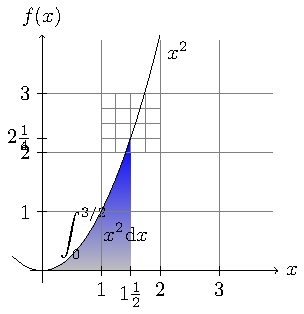
\includegraphics[width=0.7\linewidth]{mai_fig031.pdf}
      \caption{
              (\cite[s.~10000]{Feynman01})}
      \label{mai:fig031}
    \end{figure}

  \subsection{Výpočet integrálu}
      \begin{example}
        Spočítejme integrál $\displaystyle \int_1^{ln5}{(x+1)e^xdx}$  metodou per partes: 
        \begin{align*}
          \int{(x+1)e^xdx} &= \int{e^xdx}+\int{x\cdot e^xdx}     \\
                           &= e^x + (x-1)e^x = xe^x              \\
          \int_1^{ln5}{(x+1)e^xdx} &= [xe^x]_1^{ln5} = 5ln5-e    \\
        \end{align*}
        kde integrál
        \begin{align*}
            \int{xe^xdx}
              &=\left[\begin{array}{cc}
                  u=x   & dv=e^x \\ [-1em]
                  du=dx & v=e^x
                \end{array}\right]= xe^x-\int{e^xdx}  \\
              &= xe^x - e^x+C
        \end{align*}
      \end{example}

\section{Vlastnosti určitého integrálu}
  V této kapitole mluvíme o spojitých funkcích $\Rightarrow$ příslušné integrály tedy vždy
  existují. Čerpáno z knih:
  \cite{Knichal}.

  \begin{lemma}
    \textbf{První věta o střední hodnotě integrálního počtu}: Je-li funkce \(f(x)\) spojitá v
    intervalu $\langle a, b\rangle$, existuje alespoň jeden takový bod $c\in(a, b)$, že platí

    \begin{equation}\label{MA:eq_av1}
      \int_a^b f(x)dx = (b-a)f(c).
    \end{equation}
  \end{lemma}

  \begin{proof} Použitím Lagrangeovy věty napsané pro funkci \(f(x)\), primitivní na intervalu
    $\langle a, b\rangle$ k dané funkci \(f(x)\). Podmínky věty jsou zřejmě splněny: \(f(x)\) je
    spojitá na intervalu $\langle a, b\rangle$ a má všude derivaci $F'(x)= f(x)$. Tedy existuje
    alespoň jeden bod $c\in(a, b)$,
    
    \begin{figure}[ht!]  %\ref{mai:fig029}
      \centering
      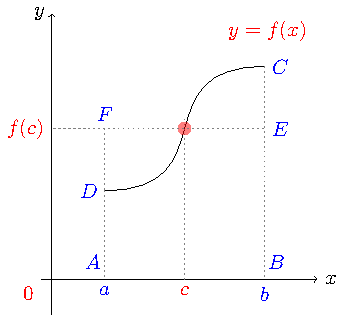
\includegraphics[width=0.7\linewidth]{mai_fig029.pdf}
      \caption{Vztah mezi silou tření a kolmou silou při smýkání
              (\cite[s.~173]{Feynman01})}
      \label{mai:fig029}
    \end{figure}

     že $$F(b)-F(a) = (b-a)F'(c),$$ čímž je věta dokázána, neboť $F(b)-F(a) = \int_a^bf(x)dx$ a
     $F'(c) = f(c)$. Funkční hodnotu $f(c)$, danou podle (\ref{MA:eq_av1}) rovnicí  
     \begin{equation}\label{MA:eq_av2}
        f(c) = \frac{1}{b-a}\int_a^b f(x)dx
     \end{equation}
     nazýváme \texttt{střední hodnotou}.
  \end{proof}

  Pro spojitou nezápornou funkci \(f(x)\), lze větu o střední hodnotě jednoduše geometricky
  interpretovat dle (obr.\ref{mai:fig029}). Levá strana (\ref{MA:eq_av1}) určuje obsah
  křivočarého lichoběžníka $ABCD$, pravá strana obsah obdélníka $ABEF$. Podle této věty nabývá
  funkce \(f(x)\) aspoň v jednom bodě intervalu $(a, b)$ takové hodnoty $f(c)$, že uvažovaný
  křivočarý lichoběžník má stejný obsah jako obdélník o základně $b-a$ a výšce $f(c)$ (str. 155
  knihy \cite{Knichal}).

  %---------------------------------------------------------------
  % !TeX spellcheck = cs_CZ
\begin{mdframed}[style=mdexam]
  \begin{example}\label{MAI:exam032}
    Určete střední hodnotu $i_s$ střídavého proudu $$i(t) = I_0\sin\omega t$$ v časovém intervalu
    $\langle 0, \frac{T}{2}\rangle$ (v průběhu jedné poloviny periody). $I_0$ je maximální hodnota
    proudu (obr. \ref{MAI:exam032}), perioda $T$ je dána vztahem $T = \frac{2\pi}{\omega}$
    
    {\centering
    \captionsetup{type=figure}
    \luafigure[1]{mai_fig030.pdf}
    \captionof{figure}{K příkladu \ref{MAI:exam032}
    \cite[s.~119]{Brabec1989}
    \label{mai:fig030}}
    \par}

      Podle \ref{MA:eq_av2} bude
      \begin{align*}
      i_s &=  \frac{2}{T}
              \int_0^{\frac{T}{2}}I_0\sin\omega t\dd{t} =
              \frac{2I_0}{T}\left[-\frac{\cos\omega t}{\omega}\right]_0^{\frac{T}{2}}        \\
          &=  \frac{2I_0}{T}\frac{1}{\omega}\left(-\cos\frac{\omega T}{2}+ \cos 0\right)     \\
          &=  \frac{2I_0}{2\pi}(-\cos\pi + \cos 0) = \frac{2}{\pi}I_0 \doteq 0,637 I_0.
    \end{align*}

    Tato hodnota se rovná intenzitě elektrického proudu, při kterém by vodičem v průběhu uvažované
    poloviny periody prošel stejný elektrický náboj jako při proudu střídavém.
  \end{example}
\end{mdframed}
















  %---------------------------------------------------------------

  %---------------------------------------------------------------
  % !TeX spellcheck = cs_CZ
\begin{mdframed}[style=mdexam]
  \begin{example}\label{MAI:exam101}
    Efektivní hodnota $i_{ef}$ střídavého proudu $$i(t) = I_0\sin\omega t$$ (viz
    předchozí příklad) je definována jako odmocnina ze střední hodnoty funkce $i^2(t)$ v průběhu
    jedné periody $T = \frac{2\pi}{\omega}$. Tedy
    \begin{align*}
      i_{ef}^2 &= \frac{1}{T}\int_0^T I_0^2\sin^2\omega t\dd{t} = 
                  \frac{1}{T}\int_0^T \frac{I_0^2}{2}(1- \cos2\omega t)\dd{t}           \\
               &= \frac{I_0^2}{2T}
                  \left[
                    t-\frac{\sin2\omega t}{2\omega}
                  \right]_0^T = \frac{I_0^2}{2}
    \end{align*}
    neboť $\sin2\omega T=\sin4\pi = 0.$ Odtud $$i_{ef} = \frac{I_0}{\sqrt{2}}.$$ Střídavý proud
    $i(t) = I_0\sin\omega t$ má na témže odporu stejný výkon jako stejnosměrný proud o intenzitě
    $i = 0,707I_0$.
  \end{example}
\end{mdframed}
















  %---------------------------------------------------------------

  Následující věta může být využita k odhadu některých integrálů
  \begin{lemma}
    \textbf{Druhá věta o střední hodnotě integrálního počtu}: Jsou-li funkce \(f(x)\) a $g(x)$
    spojité v intervalu $\langle a, b \rangle$ a je-li funkce $g(x)$ v $\langle a, b \rangle$
    nezáporná a nerostoucí, existuje alespoň jeden bod $c\in\langle a, b \rangle$ tak, že platí
    \begin{equation}\label{MA_eq_av3}
        \int_a^b f(x)g(x) = g(a)\int_a^c f(x)dx.
    \end{equation}
  \end{lemma}
  Zcela obdobnou větu lze vyslovit pro případ, že $g(x)$ je v intervalu $\langle a, b \rangle$
  nezáporná a neklesající, tj. na pravé straně \ref{MA_eq_av3} je pak integrál $g(b)\int_c^b
  f(x)dx$

   %--Odhad hodnoty integrálu \int_{100\pi}^{1000\pi}\frac{\sin x}{x}dx---------
   % !TeX spellcheck = cs_CZ
\begin{mdframed}[style=mdexam]
  \begin{example}\label{mai:exam097}
    Odhadněte hodnotu integrálu:
    \begin{equation}\label{MA_eq_sinx_x}
        \int_{100\pi}^{1000\pi}\frac{\sin x}{x}dx
    \end{equation}
    Řešení: Funkce $f(x) = \sin x$ a $g(x) = \frac{1}{x}$ jsou v uvažovaném intervalu $\langle
    100\pi, 1000\pi \rangle$ spojité a funkce $g(x)$ je kladná a nerostoucí.
    \begin{align*}
      \int_{100\pi}^{1000\pi}\frac{\sin x}{x}dx 
        &=\frac{1}{100\pi}\int_{100\pi}^c\sin xdx                                   \\
        &=\frac{1}{100\pi}\left(\cos100\pi - \cos c\right)
    \end{align*}
    kde $c$ je kladné číslo z intervalu $\langle 100\pi, 1000\pi \rangle$. Dále pro všechna
    $c\in\langle 100\pi, 1000\pi \rangle$ platí $0\leq1-\cos c\leq2$, takže
    \begin{equation*}
        0\leq\int_{100\pi}^{1000\pi}\frac{\sin x}{x}dx\leq \frac{1}{50\pi}.
    \end{equation*}
  \end{example}  
\end{mdframed}
   %----------------------------------------------------------------------------

\section{Numerický výpočet integrálu pomocí Matlabu}
  Matlab obsahuje dvě funkce pro výpočet určitého integrálu |quad| a |quadl|. Výpočet je založen na
  \emph{numerické kvadratuře}. Funkce |quad| využívá pro výpočet rekurzivní adaptivní Simpsonovo
  pravidlo. Příkaz |quad(fce,a,b)| vypočte určitý integrál funkce \emph{fce}, kde \emph{fce} je
  odkaz na funkci, \(a\) a \(b\) jsou meze integrace. Meze integrace musí být konečné. 

  Použití si ukážeme na příkladu výpočtu určitého inegrálu následující funkce
  \begin{equation*}
    \int_0^\pi x\cdot\sin{x}\dd{x}
  \end{equation*}
  Nejprve je potřeba nadefinovat funkci, kterou chceme integrovat (\(y=x\cdot\sin{x}\)), pomocí
  funkce Matlabu. Nazveme tuto funkci |int\_xsinus| a uložíme ji do zvláštního souboru 
  \begin{lstlisting}[gobble=8, style=luaMatlabStyle] 
        function [y] = int_xsinus(x)
        y = x.*sin(x);
  \end{lstlisting} 
  Výpočet integrálu pak provedeme pomocí funkce |quad(@int\_xsinus, 0, pi)|, kde první parametr je
  odkaz na funkci |int\_xsinus| a druhé dva parametry jsou meze integrace.
  \begin{lstlisting}[gobble=8, style=luaMatlabStyle] 
        >> quad(@int_xsinus, 0 , pi)
        ans = 3.1416
  \end{lstlisting}  
  Funkci je možné také definovat jako anonymní funkci, zápis se zkrátí a zpřehlední
  \begin{lstlisting}[gobble=8, style=luaMatlabStyle]  
        >> xsinus = @(x) x.*sin(x); % anonymni funkce
        >> quad(xsinus, 0, pi)      % vypocet integralu
        ans = 3.1416
  \end{lstlisting}
  Hodnota určitého integrálu na intervalu od \(0\) do \(\pi\) bude tedy \(\int_0^\pi
  x\cdot\sin{x}\dd{x} =\num{3.1416}\)

  Následující kód vypočítá hodnotu určitého integrálu zadané funkce a vykreslí graf integrované
  funkce a jejího integrálu.

  \lstinputlisting[style=luaMatlabStyle, caption=\texttt{int\_xsinus\_graph.m}: Výpis programu  
          druhého.]{../src/MAI/matlab/int_xsinus_graph.m}

  Určitý integrál je možné interpretovat jako plochu pod modrou křivkou na obrázku xx. Červená
  křivka zobrazuje hodnotu určitého integrálu v mezích od nuly do \(\pi\).

  Funkce |quadl| používá \emph{rekurzivní adaptivní Lobattovo kvadratur}. Tento postup je možné
  použí pro výpočet integrálu s větší přesností, nebo pokud integrace s |quad| selže. 

  Standardně je nastavena tolerance pro absolutní chybu menší než \num{e-6}. Tuto toleranci je možné
  změnit dalším parametrem funkcí ro integraci |quad(fce, a, b, tol)|.

%} %tikzset
%---------------------------------------------------------------------------------------------------
}
{
% DEBUG was off
\LuaPartBckgrnd{math_title02.jpg}
\LuaPartTitle{MA I}{Matematická Analýza I}{MAI}
\parttoc
%---------------------Logika a teorie množin ------------------------------------------------------
  % !TeX spellcheck = cs_CZ
%{\tikzset{external/prefix={tikz/MAI/}}
% \tikzset{external/figure name/.add={ch10_}{}}
%---------------------------------------------------------------------------------------------------
% file mai1ch01.tex
%---------------------------------------------------------------------------------------------------
\setchaptertoc
\chapter{Logika a teorie množin}\label{mai:IchapI}
  \MakeUppercase{Matematika} pochází z řeckého slova \emph{Mathema}, což znamená vědění a poznání.
  Matematika nejsou počty - ty jsou jen jedním z nástrojů, které navíc může za nás vykonat počítač.
  Je prostředkem k popisu a formalizaci jevů v okolním světě, umožňuje odhadnout důsledky těchto
  jevů a najít souvislosti mezi nimi.


  \section{Matematická logika}\label{mai:IchapIsecI}
    Vyjadřovacími prostředky matematiky, s nimiž se setkáváme v učebnicích i dalších matematických 
    textech, jsou především běžný spisovný jazyk, speciální jazyk (terminologie a symbolika) logiky 
    a matematiky, grafy, diagramy, schémata a tabulky \cite[s.~13]{polak1991matematika}.
    
    \subsection{Symboly, konstanty a proměnné}
      Velmi významné je pro matematiku užití symbolů (znaků), jež umožňuje stručné vyjadřování 
      matematických poznatků ve formě symbolických zápisů, vzorců apod. Tak např. uvažovaným 
      objektům (prvkům množin) se přiřazuje kromě názvu (jména) objektu také symbol objektu, který 
      ho zastupuje ve stručném vyjádření (v symbolických zápisech). Symbol objektu může být dvojího 
      druhu:
      \begin{enumerate}[label=\alph*), noitemsep]
        \item \textbf{Konstanta} je symbol, který označuje určitý (jediný) objekt. Z dané množiny 
              objektů. Např. 4 (označuje číslo čtyři), \(\pi\) (označuje \emph{Ludolfovo číslo}). 
        \item \textbf{Proměnná} je symbol, který označuje kterýkoli objekt z dané množiny 
              objektů. Zpravidla je to písmeno \(x\), \(y\) apod.
      \end{enumerate}
      
      Množina konstant, které zastupuje proměnná, se nazývá \textbf{obor proměnné}. Prvky oboru 
      proměnné se nazývají \emph{hodnoty proměnné}. Nahrazení proměnné konstantou z oboru 
      proměnné v nějakém výraze nazýváme \emph{dosazení konstanty za proměnnou} do daného výrazu.
    
    \subsection{Výroky a jejich pravdivostní hodnoty}
      Ze složitějších jazykových výrazů mají základní význam v logice a v matematice výroky, což 
      jsou takové jazykové výrazy (sdělení), o nichž má po obsahové stránce smysl tvrdit, že jsou 
      buď pravdivé, anebo nepravdivé (nastává právě jedna z těchto možností). Je-li \textbf{výrok 
      pravdivý}, říkáme též, že výrok platí. Je-li \textbf{výrok nepravdivý}, říká se také, že 
      výrok neplatí.
      
      Výroky, o nichž jsme (v daném okamžiku) dosud neurčili jednoznačně zda jsou pravdivé, anebo 
      nepravdivé, avšak principiálně jedna z těchto možností musí nastat, se nazývají 
      \textbf{hypotézy (domněnky)}. Gramaticky má výrok vždy formu oznamovací věty vyjádřené slovně 
      anebo symbolicky (pomocí matematických, logických, event. dalších symbolů.
      
      K označení výroků se obvykle používají malá písmena \(p\), \(q\) aj. (V literatuře se lze 
      setkat též s označením velkými písmeny.) 
      
      Výrokům se přiřazují \textbf{pravdivostní hodnoty} takto: pravdivostní hodnota \num{1} 
      (pravda), je-li výrok  pravdivý, pravdivostní hodnota \num{0} (nepravda), je-li výrok 
      nepravdivy.
      
      Příklady výroků:
      \begin{enumerate}[label=\alph*), noitemsep]
        \item \emph{Pravdivé výroky:} Bedřich Smetana je autorem hudby k opeře Prodaná 
              nevěsta. Číslo \num{10} je sudé. 
        \item \emph{Nepravdivé výroky:} Král Karel IV. nebyl korunován císařem. Každé prvočíslo 
              je liché. 
        \item \emph{Hypotézy:} Nekteré druhy rakoviny jsou vírového puvodu. Každé sudé číslo větší
              než dvě lze rozložit na součet dvou prvočísel.
      \end{enumerate}

      Mezi výroky se zařazují i taková sdělení, o jejichž pravdivosti, resp. nepravdivosti nemůžeme
      v současnosti rozhodnout, ale principiálně právě jedna z těchto možností musí nastat. Jde
      zejména o výroky, jejichž pravdivost, resp. nepravdivost je časově nebo místně podmíněná, a
      výroky vztahující se k budoucnosti:
      \begin{enumerate}[label=\alph*), noitemsep]
        \item \emph{Výroky s časove nebo místne podmínenou pravdivostí:} Prší. Jsme ve škole.
              Vyšetrujeme vlastnosti daných posloupností. 
        \item \emph{Výroky vztahující se k budoucnosti:} Zítra bude pršet. Půjdeme do kina. Daným
              bodem \(Q\) sestrojíme přímku \(q\) kolmou k dané přímce \(p\).
      \end{enumerate}

      Příklady jazykových výrazů, jež nejsou výroky:
      \begin{enumerate}[label=\alph*), noitemsep]
        \item \emph{Názvy:} stredoškolská matematika. Praha.
        \item \emph{Výrazy typu:} 2+3. 
        \item \emph{Rozkazovací a tázací věty}. 
        \item \emph{Výrazy obsahující proměnné:} Číslo \(x\) je sudé
      \end{enumerate}

      \begin{mdframed}[style=mdnote]
        \begin{note}
          Výrokům se přiřazují pravdivostní hodnoty výroku takto: Je-li výrok pravdivý, přiřazuje se
          mu pravdivostní hodnota pravda označovaná symbolem (číslicí)
          \num{1}\protect\footnotemark[2]. Je-li výrok nepravdivý, přiřazuje se mu pravdivostní
          hodnota nepravda označovaná symbolem (číslicí) \num{0}. O daném výroku se pak stručně
          říká, že má pravdivostní hodnotu \num{1}\protect\footnotemark[1], resp. \num{0}. 
        \end{note}
        \footnotetext[1]{v literatuře se lze setkat též s jejím označením \(P\)}
        \footnotetext[2]{v literatuře se lze setkat též s jejím označením \(N\)}
      \end{mdframed}
    
    \subsection{Složené výroky}  
      
      
  \section{Množiny}\label{mai:IchapIsecII}

%} %tikzset
%---------------------------------------------------------------------------------------------------
%---------------------Všemocná úměra aneb lineární algebra poprvé ---------------------------------
  % !TeX spellcheck = cs_CZ
% Basis of Linear Algebra:
%{\tikzset{external/prefix={tikz/MAI/}}
% \tikzset{external/figure name/.add={ch02_}{}}
%---------------------------------------------------------------------------------------------------
% mai1ch02.tex
%---------------------------------------------------------------------------------------------------
% ==================================================================================================
% In linear algebra, a basis is a set of linearly independent vectors that, in a
% linear combination, can represent every vector in a given vector space or free
% module, or, more simply put, which define a "coordinate system".[1] In more
% general terms, a basis is a linearly independent spanning set. 
% --------------------------------------------------------------------------------------------------
\setchaptertoc
\chapter{Všemocná úměra aneb lineární algebra poprvé}\label{mai:IchapII}

  Tuto kapitolu bychom mohli opatřit podtitulem \emph{„To nejnutnější z lineární algebry“}. Dovíme
  se v ní, co je třeba si představit pod pojmem \emph{„linearita“}, najdeme příklady linearity v
  geometrii i v přírodovědě (fyzice, chemii, biologii) a formulujeme základní poznatky týkající se
  řešení soustav lineárních rovnic. Do této oblasti patří i počítání s vektory a maticemi - objekty,
  které jsou velmi vhodné k vyjádření fyzikálních veličin.
    
  \section{Lineární rovnice}\label{mai:IchapIIsecI}
    Co tedy znamená slovo \textbf{linearita}? Pochází z latiny, \emph{linea recta = přímka}, 
    česky bychom řekli \emph{přímá úměrnost} nebo jen jednoduše \emph{úměra}.
    
    Nejjednodušší příklady linearity patří do oblasti geometrie - vyjádření \emph{přímek} a 
    \emph{rovin}. Jistě si ze střední školy vzpomínáme, že body těchto útvarů popisujeme jejich 
    souřadnicemi na přímce \(\mathbb{R}\), v rovině \(\mathbb{R}^2\), v prostoru \(\mathbb{R}^3\). 
    Souřadnice bodu v rovině tedy tvoří \emph{uspořádanou dvojici} reálných čísel, v prostoru pak 
    \emph{uspořádanou trojici} reálných čísel. (Pozor, dvojice \([a, b]\) a \([b, a]\) představují 
    různé body.)
    
    %--Parametrické vyjádření přímky--------------------------------
        % !TeX spellcheck = cs_CZ
% Musilova2009MA1
\wikitextrule
\begin{example}\label{mai:exam001}
  \textbf{Parametrické vyjádření přímky}\newline\small
  \emph{Přímka} — jednorozměrný lineární útvar v jednorozměrném prostoru \(\mathbb{R}^1\), 
  dvojrozměrném prostoru \(\mathbb{R}^2\), trojrozměrném prostoru \(\mathbb{R}^3\) (nebo i 
  n-rozměrném prostoru \(\mathbb{R}^n\)), je určena dvěma body, třeba \(A\) a \(B\), nebo 
  ekvivalentně, bodem \(A\) a \emph{směrovým} vektorem \(\vec{u}\) (obr. \ref{mai:fig000}). 
  Je-li \(X\) obecným bodem na této přímce, je vektor \(\overrightarrow{AX}\) rovnoběžný, 
  tj. \emph{kolineární}, se směrovým vektorem \(\vec{u}\). (Jako směrový můžeme samozřejmě 
  použít i vektor \(\overrightarrow{AB}\).) Vektor \(\overrightarrow{AX}\) má tedy s 
  vektorem \(\vec{u}\) stejný směr, lišit se může velikostí nebo orientací. Tuto skutečnost 
  zapíšeme tak, že \(\overrightarrow{AX}\) je \(t\)-násobkem vektorů \(\vec{u}\),
  \begin{equation*}
  \overrightarrow{AX} = t \cdot \vec{u}.
  \end{equation*}
  {\centering
    \captionsetup{type=figure}
    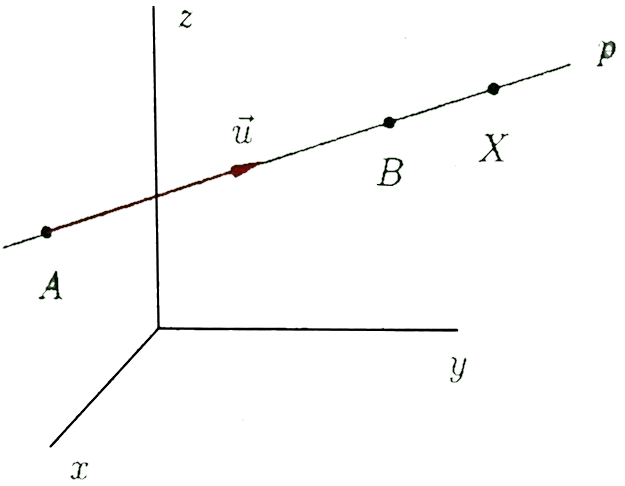
\includegraphics[width=0.4\linewidth]{mai_fig000.png}
    \captionof{figure}{Zadáni přímky. \cite[s.~1]{Musilova2009MA1}
    \label{mai:fig000}}
    \par}
  Veličinou \(t\), takzvaným \emph{parametrem}, který může nabývat všech reálných hodnot, 
  \(t\in\mathbb{R}\), dokážeme popsat všechny vektory \(\overrightarrow{AX}\), jejichž 
  koncový bod \(X\) leží na přímce \(p\). Naopak, žádné jiné body \(X\) než ty, které leží na 
  přímce \(p\), tuto vlastnost nemají. S označením bodů \(A\), \(X\), resp. vektorů 
  \(\vec{u}\), \(\overrightarrow{AX}\) kartézskými souřadnicemi, resp. složkami
  \begin{align*}
                    A &= (x_A,y_A, z_A), \\ 
                    X &=(x,y,z),         \\
              \vec{u} &= (u_1,u_2,u_3),  \\ 
  \overrightarrow{AX} &= (x - x_A, y - y_1A, z-z_A),
  \end{align*}
  dostáváme \textbf{parametrické vyjádřeni přímky} \(p\) ve tvaru
  \begin{equation}\label{MAI:eq_M001}
    p = \left\{(x,y,z)\in\mathbb{R}^3\,|\,
    \begin{matrix}
      x = x_A + tu_1,        \\
      y = y_A + tu_2,        \\
     z = z_A + tu_3,
    \end{matrix}
    \;t\in\mathbb{R}
    \right\}. 
  \end{equation}
  \normalsize
\end{example}
    %---------------------------------------------------------------

    Vidíme, že kartézské souřadnice bodu na přímce se vůči souřadnicím bodu \(A\) mění přímo 
    úměrně v závislosti na hodnotě parametru \(t\), tj. závisí na jeho první mocnině. Příslušná 
    závislost se nazývá \textbf{lineární funkcí}.

    Obdobně zapíšeme parametrické vyjádření roviny v \(\mathbb{R}^3\):
    
    %--Parametrická vyjádření roviny--------------------------------
    % !TeX spellcheck = cs_CZ
\begin{mathexam}{Parametrická vyjádření roviny}{exam004}
  Rovina v trojrozměrném prostoru \(\mathbb{R}^3\) je zadána třemi body \(A\), \(B\) a \(C\), které
  nesmějí ležet v jedné přímce, popřípadě dvěma body \(A\) a \(B\) a vektorem \(\vec{v}\)
  nerovnoběžným s \(\overrightarrow{AB}\), anebo bodem \(A\) a dvěma nerovnoběžnými směrovými
  vektory \(\vec{u}\) a \(\vec{v}\) (obr. \ref{mai:FIG002}). Všechny tyto typy zadání jsou
  ekvivalentní. Lze volit například \(\vec{u} = \overrightarrow{AB}\), \(\vec{v} =
  \overrightarrow{AC}\). Je-li \(X\) libovolným bodem roviny \(\varrho\), jsou vektory
  \(\overrightarrow{AX}\), \(\vec{u}\) a \(\vec{v}\) \textbf{lineárně závislé}. To znamená, že
  existují taková reálná čísla \(r\) a \(s\), že vektor \(\overrightarrow{AX}\) lze zapsat jako
  lineární kombinaci

  \begin{equation*}
    \overrightarrow{AX} = r\cdot\vec{u} + s\cdot\vec{v}, \qquad r,s \in\mathbb{R}
  \end{equation*}
  Při obdobném zápisu kartézských souřadnic bodů a složek vektorů jako u vyjádření přímky dostaneme
  parametrické vyjádření roviny \(\varrho\)
  \begin{equation*}
    \varrho = \left\{
    \begin{matrix}  
      (x,y,z)\in\mathbb{R}^3  \\
      r, s \in\mathbb{R}
    \end{matrix}
    \,\left\lvert\,
    \begin{matrix}
      x = x_A + ru_1 + sv_1,        \\
      y = y_A + ru_2 + sv_2,        \\
      z = z_A + ru_3 + sv_3,
    \end{matrix}\right.          
    \right\}.
  \end{equation*} 

  { \centering
    \captionsetup{type=figure}
    \luafigure[1]{mai_fig026.pdf}
    \captionof{figure}{Zadání roviny. \cite[s.~3]{Musilova2009MA1}
    \label{mai:FIG002}} \par}

  Toto vyjádření obsahuje opět lineární závislost: Souřadnice \(x\), \(y\) a \(z\) se vůči
  souřadnicím bodu \(A\) mění v závislosti na prvních mocninách parametrů \(r\) a \(s\). Můžeme tak
  hovořit o jakési „vícerozměrné úměře“.
\end{mathexam}
  
    %---------------------------------------------------------------

    Všimněme si nyní příkladů linearity z oblasti přírodovědy.
    
    %--Fyzika - Ohmův zákon-----------------------------------------
    % !TeX spellcheck = cs_CZ
% \wikitextrule
\begin{mdframed}[style=mdexam]
  \begin{example}\label{mai:exam035}
    \textbf{Fyzika - Ohmův zákon:}\newline
    Z elektřiny víme, že některé vodiče či elektrické prvky se při průchodu elektrického proudu 
    chovají podle zákona linearity: Proud, který jimi protéká, závisí přímo úměrně na přiloženém 
    napětí (obr. \ref{mai:fig036}). Platí \(I(U) = R^{-1 }U\) s konstantou úměrnosti \(R^{-1}\), kde 
    \(R\) je elektrický odpor vodiče (prvku).

    Pozn. 1: Předpokládáme, že elektrický odpor voltmetru je tak velký, že proud jím procházející je 
    z hlediska přesnosti měření zanedbatelný.
    
    Pozn. 2: Graf závislosti proudu na napětí na obrázku \ref{mai:fig036} může pro vyšší hodnoty 
    napětí vykazovat odchylku od linearity (přímkové závislosti), neboť se prvek při vyšším proudu 
    zahřívá a jeho odpor roste.
    
    {\centering
      \captionsetup{type=figure}
      \luafigure[1]{mai_fig036.png}
      \captionof{figure}{Chování lineárního vodiče (Ohmův zákon). \cite[s.~15]{Musilova2009MA1}
      \label{mai:fig036}}
      \par}  
  \end{example}
\end{mdframed}
    %---------------------------------------------------------------

    %--Fyzika - speciální typy pohybů-------------------------------
    % !TeX spellcheck = cs_CZ
\wikitextrule
\begin{example}\label{mai:exam036}
  \textbf{Fyzika — speciální typy pohybů:}\newline\small
  Při rovnoměrném pohybu tělesa (ať již přímočarém či křivočarém) je dráha, kterou těleso urazí za 
  dobu \(t\), přímo úměrná velikosti jeho rychlosti \(v\), tj. \(s(t) = s_0 + vt\). Při pohybu 
  rovnoměrně zrychleném (zpožděném) je lineární závislost velikosti rychlosti na čase, tj. \(v(t) = 
  v_0 \pm at\) při pohybu přímočarém (\(a\) je velikost zrychlení), nebo \(v(t) = v_0 \pm a_\tau 
  t\) při pohybu křivočarém (\(a_\tau\) je velikost průmětu zrychlení do směru tečny k 
  trajektorii tělesa — tečného zrychlení).
  \normalsize
\end{example}
    %---------------------------------------------------------------
    
    \subsection{Soustavy lineárních rovnic a jejich rychlé řešení}\label{mai:IchapIIsecIssecI}
      Příkladů linearity v přírodě bychom mohli nalézt bezpočet. Vraťme se však k matematice a k
      problematice uvedené v názvu tohoto odstavce, k soustavám lineárních rovnic. Začněme
      jednoduchou slovní úlohou ze základní školy:
      
      %--Jeníček a Mařenka kradli ježibabě perník---------------------
      % !TeX spellcheck = cs_CZ
% \wikitextrule
\begin{mdframed}[style=mdexam]
  \begin{example}\label{mai:exam037}
    \textbf{Jeníček a Mařenka kradli ježibabě perník:}\newline
    Dohromady snědli \num{11} perníkových srdíček. Jeníček jich přitom zkonzumoval o \num{3} více
    než Mařenka. Otázka je tradiční - kolik srdíček snědl každý z nich? Označíme-li \(M\) počet
    kousků, které snědla Mařenka a \(J\) počet srdíček, na nichž si pochutnal Jenda, můžeme
    informace zadané v úloze zapsat takto:
    \begin{equation*}
      M + J = 11, \qquad J = M + 3.
    \end{equation*}
    
    Řešení není problémem, snadno vidíme, že \(M = 4\) a \(J = 7\).
  \end{example}
\end{mdframed}
      %---------------------------------------------------------------
      
      O samotné řešení této jednoduché úlohy v tuto chvíli nejde. Pojmenujme si však vztahy, které
      jsme pro neznámé hodnoty \(M\) a \(J\) ze zadání úlohy dostali. Neznámé vystupují v rovnicích
      v první mocnině, tedy \emph{lineárně}. Máme \emph{soustavu dvou rovnic} o dvou neznámých \(M\)
      a \(J\). Úvahu snadno zobecníme: Předpokládejme, že máme neznámé veličiny
      \begin{equation*}
        (x_1, x_2, \ldots, x_n)
      \end{equation*}
      a máme o nich \(m\) informací, které lze zapsat ve tvaru lineárních rovnic (neznámé budou v
      těchto rovnicích vystupovat v první mocnině),
      \begin{align}
        a_{11}x_1 + a_{12}x_2 + \ldots + a_{1n}x_n &= b_1,     \nonumber           \\
        a_{21}x_1 + a_{22}x_2 + \ldots + a_{2n}x_n &= b_2,     \label{mai:eq002}   \\
        .......................................... &= \ldots   \nonumber           \\
        a_{m1}x_1 + a_{m2}x_2 + \ldots + a_{mn}x_n &= b_m,     \nonumber
      \end{align}
      Soustavu (\ref{mai:eq002}) \textbf{nazýváme soustavou \(\mathbf{m}\) lineárních rovnic o
      \(\mathbf{n}\) neznámých}. Označme ji jako \(S\) a pod tímto označením se k ní budeme vracet.
      Soubory reálných čísel \((a_{ij})\) a \((b_i)\), kde \(1 \leq i \leq m\), \(1 \leq j \leq n\),
      jsou zadány. Lze je uspořádat do takzvaných \textbf{matic}:
      \begingroup
        \renewcommand\arraycolsep{3pt}
        \begin{equation*}
          \matr{A} =
            \begin{pmatrix}[0.9]
              a_{11} & a_{12} & \ldots & a_{1n} \\
              a_{21} & a_{22} & \ldots & a_{2n} \\
              \ldots & \ldots & \ldots & \ldots \\
              a_{m1} & a_{m2} & \ldots & a_{mn}          
            \end{pmatrix},\quad
            \overline{\matr{B}} =
            \begin{pmatrix}[0.9]
              b_1     \\
              b_2     \\
              \ldots  \\
              b_m 
            \end{pmatrix}
        \end{equation*}
      \endgroup

      Matice \(\matr{A}\) je typu \(m/n\), má \(m\) řádků a \(n\) sloupců, \(i\) je řádkový index a
      \(j\) je sloupcový index. Matice \(\overline{\matr{B}}\) je typu \(m/1\) (\(m\) řádků a jeden
      sloupec), hovoříme také o sloupcové matici. Soustavu \(S\) můžeme zapsat zkráceně pomocí
      maticového násobení (podrobněji viz později odstavec \ref{mai:IchapIIsecIII}):
      \begin{align}\label{mai:eq004}
        \matr{A} \cdot \matr{X} &= \overline{\matr{B}}, \quad \text{nebo} \nonumber\\
        \setlength{\arraycolsep}{3pt}
          \begin{pmatrix}[0.9]
            a_{11} & a_{12} & \ldots & a_{1n} \\
            a_{21} & a_{22} & \ldots & a_{2n} \\
            \ldots & \ldots & \ldots & \ldots \\
            a_{m1} & a_{m2} & \ldots & a_{mn}
          \end{pmatrix} \cdot
          \begin{pmatrix}[0.9]
            x_1     \\
            x_2     \\
            \ldots  \\
            x_m 
          \end{pmatrix}  &=
          \begin{pmatrix}[0.9]
            b_1     \\
            b_2     \\
            \ldots  \\
            b_m 
          \end{pmatrix}
      \end{align} 
      V tuto chvíli vysvětlíme podstatu maticového násobení jen technicky: Násobit mezi sebou
      můžeme matici \(\matr{A} = (a_{ij})\) typu \(m/n\) (levý činitel) a matici \(\matr{C} =
      (c_{jk})\) typu \(n/p\) (pravý činitel, činitele nelze zaměňovat). Výsledkem je matice
      \(\matr{D} = (d_{ik})\) typu \(m/p\), jejíž prvky se počítají podle předpisu
      \begin{equation}\label{mai:eq005}
        d_{ik} = \sum_{j=1}^{n} a_{ij}\cdot c_{jk}.
      \end{equation}
      
      Z tohoto obecného předpisu vidíme, že levé strany soustavy \(S\) lze interpretovat ve tvaru
      součinu matice \(A\) typu \(m/n\) s maticí neznámých typu \((n/1)\), výsledkem je matice
      pravých stran \(\overline{\matr{B}}\), která je typu \(m/1\). Matice \(\matr{A}\) se nazývá
      \textbf{maticí soustavy}. Matice, která vznikne jejím \emph{rozšířením} o sloupec pravých
      stran, tj.
      \begingroup
        \renewcommand\arraystretch{0.8}
        \renewcommand\arraycolsep{3pt}
        \begin{equation*}
          \matr{B} = (\matr{A}\lvert\overline{\matr{B}}) =
          \left(
            \begin{array}{cccc|c}
              a_{11} & a_{12} & \ldots & a_{1n} & b_1    \\
              a_{21} & a_{22} & \ldots & a_{2n} & b_2    \\
              \ldots & \ldots & \ldots & \ldots & \ldots \\
              a_{m1} & a_{m2} & \ldots & a_{mn} & b_m 
            \end{array}
          \right)
        \end{equation*}
      \endgroup
      je pak \textbf{rozšířenou maticí soustavy}. Je-li sloupec pravých stran soustavy tvořen samými
      nulami, nazývá se soustava \textbf{homogenní}, v opačném případě \textbf{nehomogenní}. Řešením
      soustavy \(S\) nazýváme každou \(n\)-tici \((x_i, x_2,\ldots, x_n)\), která soustavu \(S\)
      splňuje. Cílem je najít všechna řešení soustavy \(S\). Abychom řešení nalezli, musíme soustavu
      upravovat, zjednodušovat. Prováděné úpravy mají vést k jednodušší, avšak ekvivalentní soustavě
      rovnic, tj. takové, která má naprosto stejný soubor všech řešení jako soustava původní. Takové
      úpravy nazýváme \textbf{ekvivalentními}. Dvě základní, pomocí nichž lze uskutečnit všechny
      ostatní, jsou
      \begin{mdframed}[style=highlight]
        \begin{itemize}[noitemsep]
          \item vynásobení libovolné, například \(i\)-té, rovnice libovolným \emph{nenulovým}
                číslem,
          \item přičtení \(i\)-té rovnice vynásobené libovolným číslem k \(l\)-té rovnici.
        \end{itemize} 
      \end{mdframed}
      V soustavě lze samozřejmě také měnit pořadí rovnic. Tato úprava je rovněž ekvivalentní.
      Nevypisujeme ji však zvlášť proto, že ji lze realizovat pomocí vhodně zvolené posloupnosti
      základních dvou úprav.
      
      Abychom nemuseli soustavu stále opisovat i s neznámými, provádíme obvykle ekvivalentní úpravy
      jen s maticí \(\matr{B} = (\matr{A}\vert\overline{\matr{B}})\) (každý řádek této matice
      představuje jednu rovnici soustavy \(S\)). Může se stát, že soustava má právě \emph{jedno
      řešení}, jako tomu bylo v  úloze o Mařence a Jeníčkovi. Také nemusí mít \emph{řešení žádné},
      jako například soustava \(x + y = 0\), \(x + y = 1\) (součet dvou čísel nemůže nabývat
      současně dvou různých hodnot). A třeba má také řešení \emph{nekonečně mnoho} (řešením soustavy
      jedné rovnice o dvou neznámých \(x + y = 1\) jsou všechny dvojice tvaru \((x, 1 - x)\), kde
      \(x\) je libovolné). A může mít soustava \(S\) třeba právě dvě řešení? Prostřednictvím
      následujícího příkladu ukážeme metodu, která vede velmi rychle k nalezení všech řešení a
      umožňuje také vyslovit obecné závěry o jejich vlastnostech a počtu. Jedná se o
      \textbf{Gaussovu eliminační metodu}.

      %Gaussova eliminační metoda-------------------------------------
      \begin{mathexam}{Gaussova eliminační metoda}{exam038}
  Je zadána soustava tří (\(m = 3\)) rovnic o pěti (\(n = 5\)) neznámých:
  \begin{alignat*}{7}
       x_1 &+ 2x_2 &-  x_3 &+  x_4 &- 5x_5 &=  &&0, \\
     -2x_1 &- 4x_2 &+ 2x_3 &+ 4x_4 &+ 4x_5 &= -&&6, \\
      -x_1 &- 2x_2 &+  x_3 &+ 5x_4 &-  x_5 &=  &&6.
  \end{alignat*}
  Budeme provádět ekvivalentní úpravy matice \(\matr{B}\) tak, abychom ji zjednodušovali.
  Ekvivalenci matic budeme označovat znakem \(\sim\). 
  \begingroup
    \renewcommand\arraystretch{1.0}
    \renewcommand\arraycolsep{3pt}
    \begin{equation*}
      \matr{B} = (\matr{A}\lvert\overline{\matr{B}}) =
      \left(
        \begin{array}{rrrrr|r}
           1 &  2 & -1 & 1 & -5 &  0    \\
          -2 & -4 &  2 & 4 &  4 & -6    \\
          -1 & -2 &  1 & 5 & -1 &  6
        \end{array}
      \right).
    \end{equation*}
  \endgroup
  V prvním řádku je na první pozici jednička. Toho využijeme k snadné „likvidaci“, tedy eliminaci,
  prvních prvků v druhém a třetím řádku pomocí elementárních úprav. Provedeme tyto dvě úpravy:
  první řádek vynásobený číslem \num{2} přičteme k druhému řádku, první řádek přičteme ke třetímu
  řádku. Dostaneme
  \begingroup
    \renewcommand\arraystretch{1.0}
    \renewcommand\arraycolsep{3pt}
    \begin{equation*}
      \matr{B} \sim
      \left(
        \begin{array}{rrrrr|r}
          1 &  2 & -1 & 1 & -5 &  0         \\
          \bm{0} &  0 &  0 & 6 & -6 & -6    \\
          \bm{0} &  0 &  0 & 6 & -6 &  6
        \end{array}
      \right).
    \end{equation*}
  \endgroup  
  Vidíme, že jsme v druhém i třetím řádku dostali na první sloupcové pozici nulu (tučná). (Nuly na
  dalších  pozicích vznikly náhodou, vlivem jednoduchosti zadání.) Nyní vynásobíme druhý i třetí
  řádek číslem (\num{1/6}):
  \begingroup
    \renewcommand\arraystretch{1.0}
    \renewcommand\arraycolsep{3pt}    
    \begin{equation*}
      \matr{B} \sim
      \left(
        \begin{array}{rrrrr|r}
                1 &  2 & -1 & 1 & -5 &  0    \\
                0 &  0 &  0 & 1 & -1 & -1    \\
                0 &  0 &  0 & 1 & -1 &  1
        \end{array}
      \right).
    \end{equation*}
  \endgroup  
  Přestože již nyní vidíme, že soustava nemá řešení (rovnice druhého a třetího řádku znějí \(x_4 -
  x_5 = - 1\) a \(x_4 -x_5 = 1\), takže jim nevyhovuje žádná dvojice čísel \((x_4, x_5)\)), budeme
  v eliminaci pokračovat. Další úpravy se již týkají pouze druhého a třetího řádku. Druhý řádek
  vynásobený (\num{-1}) přičteme ke třetímu. Pak

  \begingroup
  \renewcommand\arraystretch{1.0}
  \renewcommand\arraycolsep{3pt}
    \begin{equation*}
      \matr{B} \sim
      \left(
        \begin{array}{rrrrr|r}
                1 &  2 & -1 & 1      & -5 &  0    \\
                0 &  0 &  0 & 1      & -1 & -1    \\
                0 &  0 &  0 & \bm{0} &  0 &  2
        \end{array}
      \right).
    \end{equation*}
  \endgroup  
  Získáváme tak ekvivalentní soustavu rovnic
  \begin{alignat*}{5}
        x_1 + 2x_2 - x_3 &+  x_4 &- 5x_5 &=  &&0, \\
                         &+  x_4 &-  x_5 &= -&&1, \\
                         &       &     0 &=  &&2.
  \end{alignat*}
  V poslední rovnici je ihned vidět rozpor - soustava nemá řešení
\end{mathexam}
      %---------------------------------------------------------------

      Na základě výsledného tvaru matice soustavy a rozšířené matice soustavy získané ekvivalentními
      úpravami soustavy \(S\) nyní formulujeme obecné kritérium pro to, aby soustava S měla vůbec
      nějaké řešení. Matice \(\matr{A}\) i \(\matr{B}\) se po provedení ekvivalentních úprav dostaly
      do velmi jednoduchého tvaru, který připomíná schodiště obrácené „vzhůru nohama“, odmyslíme-li
      si nuly v levé části jednotlivých řádků (následující zápis pouze usnadňuje názornou představu,
      znak ekvivalence již psát nemůžeme):
      \begingroup
        \renewcommand\arraystretch{0.9}
        \renewcommand\arraycolsep{3pt}
        \begin{align*}
          \matr{A} &\ldots
          \left(
            \begin{array}{rrrrr}
                    1 &  2 & -1 & 1      & -5     \\
                      &    &    & 1      & -1 
            \end{array}
          \right),  \\
          \matr{B} &\ldots
          \left(
            \begin{array}{rrrrr|r}
                    1 &  2 & -1 & 1      & -5 &  0    \\
                      &    &    & 1      & -1 & -1
            \end{array}
          \right).
        \end{align*}
      \endgroup

      Všimněme si, že „schodiště“ jsou nepravidelná, pokud jde o šířku schodů, výška všech schodů je
      však stejná - jeden řádek. Tímto způsobem je dán \emph{schodovitý tvar} matice \(\matr{A}\),
      resp. \(\matr{B}\). Úzce s ním souvisí důležitá charakteristika matice, která je nezávislá jak
      na provedených úpravách tak na výsledném schodovitém tvaru. Je to hodnost matice, definovaná
      takto:      
      \begin{mdframed}[style=highlight] 
        \textbf{Hodnost} matice je počet nenulových řádků jejího schodovitého tvaru.
      \end{mdframed}
      V našem příkladu je hodnost matice \(\matr{A}\) soustavy \(S\) rovna dvěma, hodnost matice
      rozšířené \(\matr{B}\) je rovna třem. Píšeme
      \begin{equation*}
        h(\matr{A}) = 2,\qquad h(\matr{B}) = 3.
      \end{equation*}
      
      \begin{mdframed}[style=mdnote] 
        \begin{note}
          Že lze získat schodovitý tvar různými posloupnostmi ekvivalentních úprav je zřejmé. Uvědomme
          si však, že ani výsledný schodovitý tvar není určen jednoznačně - stačí třeba vynásobit
          některý řádek dvěma a výsledná matice ekvivalentní s původní je rovněž schodovitá. Poněvadž
          má matice \(\matr{B}\) o jeden sloupec více než matice \(\matr{A}\), platí vždy
          \(h(\matr{A}) < h(\matr{B})\). V případě \(h(\matr{A}) < h(\matr{B})\) pak \(h(\matr{A}) =
          h(\matr{B}) - 1\). Jak názorně ukazuje náš příklad, má pro \(h(\matr{A}) < h(\matr{B})\)
          některá z rovnic ekvivalentní soustavy tvar \(0 = 1\), soustava tedy nemá řešení. Můžeme tak
          formulovat kritérium (podmínku nutnou a postačující) řešitelnosti soustavy lineárních
          rovnic.
        \end{note}
      \end{mdframed}
      
      \begin{lemma}\label{mai:lemma001}
        (\textbf{Frobeniova}): Soustava lineárních rovnic má řešení právě tehdy, je-li hodnost její
        matice rovna hodnosti matice rozšířené.
      \end{lemma}
      
      Ihned vidíme, že homogenní soustava má podle této věty řešení vždy, neboť poslední sloupec
      její rozšířené matice je složen ze samých nul. Skutečně, jedním ze souboru řešení každé
      homogenní soustavy je \(n\)-tice
      \begin{equation*}
        (x_1, x_2, \ldots, x_n) = (0, 0, \ldots, 0),
      \end{equation*}
      zvaná \textbf{triviální řešení}.
      
      Nyní se vraťme k otázce, jak zjistit, kolik řešení má daná soustava, a jak je všechna popsat.
      Poslouží nám příklad \ref{mai:exam038} v mírné obměně spočívající v záměně koeficientu \(b_3\)
      z hodnoty \num{6} na \num{-6}.
      
      %Ještě jednou Gaussova eliminační metoda------------------------
      % !TeX spellcheck = cs_CZ
\wikitextrule
\begin{example}\label{mai:exam039}
  \textbf{Ještě jednou Gaussova eliminační metoda}\newline\small
  Je zadána soustava rovnic:
  \begin{alignat*}{7}
      x_1 &+ 2x_2 &-  x_3 &+  x_4 &- 5x_5 &=  &&0, \\
    -2x_1 &- 4x_2 &+ 2x_3 &+ 4x_4 &+ 4x_5 &= -&&6, \\
     -x_1 &- 2x_2 &+  x_3 &+ 5x_4 &-  x_5 &= -&&6.
  \end{alignat*}
  Rozšířená matice soustavy má nyní tvar 
  \begin{equation*}
    \matr{B} = (\matr{A}|\overline{\matr{B}}) =
    \left(
      \begin{array}{rrrrr|r}
         1 &  2 & -1 & 1 & -5 &  0    \\
        -2 & -4 &  2 & 4 &  4 & -6    \\
        -1 & -2 &  1 & 5 & -1 & -6
      \end{array}
    \right).
  \end{equation*}
  Stejné ekvivalentní úpravy jako v příkladu \ref{mai:exam038} vedou nyní k výsledku
  \footnotesize %\small \scriptsize \tiny
  \begin{equation*}
    \matr{B} \sim
    \left(
      \begin{array}{rrrrr|r}
         1 &  2 & -1 & 1 & -5 &  0         \\
         \bm{0} &  0 &  0 & 6 & -6 & -6    \\
         \bm{0} &  0 &  0 & 6 & -6 & -6
      \end{array}
    \right) \sim
    \left(
      \begin{array}{rrrrr|r}
              1 &  2 & -1 & 1 & -5 &  0    \\
              0 &  0 &  0 & 1 & -1 & -1    \\
              0 &  0 &  0 & 1 & -1 & -1
      \end{array}
    \right) \sim
    \left(
      \begin{array}{rrrrr|r}
              1 &  2 & -1 & 1      & -5 &  0    \\
              0 &  0 &  0 & 1      & -1 & -1    \\
              0 &  0 &  0 & \bm{0} &  0 &  0
      \end{array}
    \right).
  \end{equation*}\normalsize
  Nyní platí \(h(\matr{A}) = h(\matr{B}) = 2\). Podle Frobeniovy věty \ref{mai:lemma001} tedy 
  soustava určitě má řešení. Ekvivalentní soustava má tvar
  \begin{alignat*}{5}
         x_1 + 2x_2 - x_3 &+  x_4 &- 5x_5 &=  &&0, \\
                          &+  x_4 &-  x_5 &= -&&1, \\
                          &       &     0 &=  &&0.
  \end{alignat*}
  Poslední rovnice je identitou a můžeme ji vypustit. Máme pět neznámých a jen dvě nezávislé 
  rovnice. Dvě z neznámých tedy můžeme vyjádřit pomocí zbývajících. Postupujeme „odzadu“ , začínáme 
  druhou, jednodušší, rovnicí:
  \begin{align*}
                                                x_4 &= -1 + x_5,                \\
    x_1 = - 2x_2 + x_3 - x_4 + 5x_5 \Rightarrow x_1 &= -2x_2 + x_3 + 4x_5 + 1.
  \end{align*}
  Za neznámé vystupující na pravé straně, tj. \(x_2\), \(x_3\) a \(x_5\), můžeme dosazovat cokoli a 
  vždycky se k nějakým hodnotám \(x_1\) a \(x_4\) dopočítáme. Všechna řešení soustavy \(S\) proto 
  můžeme zapsat v obecném tvaru
  \begin{equation}\label{mai:eq040}
    (-2x_2 + x_3 + 4x_5 + 1, x_2, x_3, x_5 - 1, x_5).
  \end{equation}
  \normalsize
\end{example}
      %---------------------------------------------------------------
      
      Soubor řešení ve tvaru (\ref{mai:eq040}) se nazývá obecným řešením soustavy. Jeho jednotlivé
      prvky, jednotlivá konkrétní řešení soustavy, jsou dány volbou volných neznámých \(x_2\),
      \(x_3\) a \(x_5\). Také z příkladu \ref{mai:exam039} lze učinit obecný závěr:
      
      \begin{lemma}\label{mai:lemma002}
        Nechť pro soustavu \(m\) lineárních rovnic o \(n\) neznámých platí \(h(\matr{A}) =
        h(\matr{B}) = h\). Pak její obecné řešení závisí (lineárně) na \(d = n - h\) volných
        neznámých.
      \end{lemma}
      
      Číslo \(d\) se nazývá \textbf{dimenze prostoru řešení soustavy}. Tento pojem ještě podrobněji
      vysvětlíme později.
      
      Nyní již snadno zodpovíme otázku, čím je dána \emph{mohutnost souboru řešení soustavy
      lineárních rovnic}, tj. kolik má taková soustava řešení. Možnosti jsou pouze:
      \begin{mdframed}[style=highlight]
        \begin{itemize}[leftmargin=3pt,noitemsep]
          \item žádné řešení - pro \(h(\matr{A}) \neq h(\matr{B})\),
          \item právě jedno řešení - pro \(h = h(\matr{A}) = h(\matr{B})\) a současně \(h = n\),
                takže nezbývá žádná volná neznámá,
          \item nekonečně mnoho řešení - pro \(h = h(\matr{A}) = h(\matr{B})\) a současně \(h < n\),
                kdy máme k dispozici \(d = n - h\) volných neznámých.
        \end{itemize}  
      \end{mdframed}  
      Že by tedy třeba měla soustava právě dvě, tři či osmnáct řešení není možné.
      
      Jakési zvláštní postavení můžeme přisoudit \emph{homogenním soustavám}. Ty mají, jak jsme se
      již přesvědčili, řešení vždy, alespoň to triviální, složené ze samých nul. Zajímejme se o
      situaci, kdy má homogenní soustava i jiná, netriviální, řešení. U homogenní soustavy je
      hodnost její matice vždy shodná s hodností matice rozšířené, \(h = h(\matr{A}) =
      h(\matr{B})\). Je-li navíc \(h = n\), má podle obecného tvrzení \ref{mai:lemma002} soustava
      právě jedno řešení, jímž nutně je řešení triviální. V opačném případě, tj. pro \(h < n\), máme
      opět k dispozici \(d = n - h\) volných neznámých, a tedy nekonečně mnoho netriviálních řešení.
      Všimněme si ještě jedné zajímavosti u homogenní soustavy. Jsou-li dvě \(n\)-tice čísel \(X =
      (x_1, x_2, \ldots, x_n)\) a \(\overline{X} = (\overline{x}_1, \overline{x}_2, \ldots,
      \overline{x}_n)\) jejím řešením, pak také \(n\)-tice vytvořená jako jejich lineární kombinace
      \begin{equation*}
        \alpha\cdot X + \overline{\alpha}\cdot\overline{X} = 
          (\alpha x_1, \alpha x_2, \ldots, \alpha x_n) + 
          (\overline{\alpha}\,\overline{x}_1, 
          \overline{\alpha}\,\overline{x}_2, \ldots, 
          \overline{\alpha}\,\overline{x}_n)
      \end{equation*}
      kde \(\alpha\) a \(\overline{\alpha}\) jsou libovolná čísla, je \emph{řešením soustavy}.
      Možnost tohoto „lineárního kombinování“ připadá samozřejmě v úvahu pro libovolný počet
      libovolných řešení soustavy. Fyzik by řekl, že soustava vyhovuje principu superpozice.
      Soustava nehomogenní tu to vlastnost nemá „vinou“ nenulového sloupce pravých stran.
    
    \subsection{Přímky a roviny - lineární geometrické útvary}
      Vraťme se ještě na chvíli k linearitě v geometrii a všimněme si problematiky vzájemné polohy
      přímek a rovin. Procvičíme si na ní mimo jiné i řešení soustav lineárních rovnic. V odstavci
      \ref{mai:IchapIIsecIssecI} jsme odvodili parametrické vyjádření přímky a roviny v
      trojrozměrném prostoru. Nyní se pokusíme z těchto vyjádření vyloučit parametry a získat obecné
      rovnice přímky a roviny, které již budou obsahovat pouze kartézské souřadnice bodů ležících v
      příslušné přímce či rovině. Začněme případem roviny.

      %--Obecná rovnice roviny----------------------------------------
      % !TeX spellcheck = cs_CZ
\wikitextrule
\begin{example}\label{mai:exam040}
  \textbf{Obecná rovnice roviny}\newline\small
  Parametrické rovnice roviny z příkladu \ref{mai:exam004} můžeme chápat jako soustavu tří rovnic o 
  dvou neznámých:
  \begin{align*}
      ru_1 + sv_1 &= x - x_A, \\
      ru_2 + sv_2 &= y - y_A, \\
      ru_3 + sv_3 &= z - z_A, 
  \end{align*}
  kde neznámými jsou parametry \(r\) a \(s\). Z geometrického významu této soustavy je zřejmé, že 
  pro každý bod \(X = (x, y, z)\), který leží v rovině \(\varrho\), bude soustava mít jako řešení 
  právě jednu dvojici parametrů \((r, s)\) (pro body, které v rovině neleží, soustava řešení nemá). 
  Vypočteme parametry \(r\) a \(s\) například z prvních dvou rovnic. Předpokládejme, že \(u_1 \neq 
  0\), a upravujme matici soustavy:
  
  \begin{equation*}
    \left(
      \begin{array}{rr|r}
         u_1 &  v_1  &  x-x_A         \\
         u_2 &  v_2  &  y-y_A
      \end{array}
    \right) \sim
    \left(
      \begin{array}{cc|c}
              u_1 &  v_1               & x - x_A     \\
              0   &  u_1v_2 - u_2v_1   & (y-y_A)u_1 - (x-x_A)u_2
      \end{array}
    \right).
  \end{equation*}
  odkud pro \((u_1v_2 — u_2v_1) \neq 0\) dostaneme
  \begin{equation*}
    r = - \dfrac{(y-y_A)v_1 - (x-x_A)v_2}{u_1v_2 - u_2v_1}, \qquad 
    s =   \dfrac{(y-y_A)u_1 - (x-x_A)u_2}{u_1v_2 - u_2v_1}
  \end{equation*}
  Dosadíme-li získané hodnoty do třetí rovnice (dá to trochu práce), dostáváme obecnou  rovnici roviny 
  \(\varrho\)
  \begin{subequations} % \label{mai:eq041}
    \begin{equation}\label{mai:eq041a}
      ax + by + cz + d= 0,
    \end{equation}
    \begin{equation}\label{mai:eq04b}
      a = u_2v_3 - u_3v_2, \qquad b = u_3v_1 - u_1v_3, \qquad c = u_1v_2 - u_2v_1,
    \end{equation}
    \begin{equation}\label{mai:eq041c}
      d = (u_2v_3 - u_3v_2)x_A - (u_3v_1 - u_1v_3)y_A - (u_1v_2 - u_2v_1)z_A.
    \end{equation}
  \end{subequations}
  Při tomto výpočtu vyvstaly některé problémy. Pokusme se je vyřešit:
  \begin{itemize}
    \item Aby získaná rovnice opravdu představovala nějakou rovinu, musí v ní zůstat alespoň jedna 
          ze souřadnic \(x, y, z\). Alespoň jedno z čísel \(a, b, c\) by tedy mělo být nenulové. 
          Dokažte, že tomu tak opravdu je, a využijte při tom skutečnosti, že vektory \(\vec{u}\) a 
          \(\vec{v}\) nesmí být rovnoběžné. Co znamená předpoklad \((u_1v_2 - u_2v_1) \neq 0\)?
    \item Předpokládali jsme, že \(u_1 \neq 0\). Jak budeme postupovat, nebude-li tento předpoklad  
          splněn? Lze v tomto případě použít obecné výrazy získané pro \(r\) a \(s\)?
  \end{itemize}
  \normalsize
\end{example}
      %---------------------------------------------------------------

      %--Obecná rovnice přímky----------------------------------------
      % !TeX spellcheck = cs_CZ
% \wikitextrule
\begin{mdframed}[style=mdexam]
  \begin{example}\label{mai:exam041}
    \textbf{Obecná rovnice přímky}\newline
    Přímku \(p\) si snadno představíme jako průsečnici dvou nerovnoběžných rovin \(\varrho\) a 
    \(\sigma\). Jejich rovnice tvoří soustavu, která představuje obecné rovnice přímky
      \begin{align*}
        \varrho &= \{(x, y, z)\in\mathbb{R}^3\mid a_1x+ b_1y+ c_1z+ d_1 = 0 \}  \\ 
        \sigma  &= \{(x, y, z)\in\mathbb{R}^3\mid a_2x+ b_2y+ c_2z+ d_2 = 0 \}, 
      \end{align*}
    Zkusme přijít na to, co musí platit pro koeficienty v rovnicích rovin, aby byly nerovnoběžné. 
    Jedna a táž přímka může být zadána různými dvojicemi nerovnoběžných rovin. Všechny roviny, které 
    přímkou \(p\) procházejí, tvoří geometrický útvar zvaný \textbf{svazek rovin prvního druhu}, 
    přímka sama je \textbf{osou} svazku. 
  \end{example}
\end{mdframed}
      %---------------------------------------------------------------
      
      %--Vektor rovnoběžný s rovinou----------------------------------
      % !TeX spellcheck = cs_CZ
\wikitextrule
\begin{example}\label{mai:exam042}
  \textbf{Vektor rovnoběžný s rovinou}\newline\small
   Ja k poznáme, zda je vektor \(\vec{u} = (u_1, u_2, u_3)\) rovnoběžný s rovinou \(ax + by + cz + 
   d = 0\)? Pokud vektor \(\vec{u}\) s rovinou rovnoběžný je, pak zcela jistě existují v této 
   rovině dva body \(A = (x_A, y_A, z_A)\) a \(B = (x_B, y_B, z_B)\) tak, že \(\overrightarrow{AB} 
   = \vec{u} = (x_B - x_A, y_B - y_A, z_B - z_A)\). Tyto body splňují rovnici roviny, tj.
   \begin{equation*}
     ax_A + by_A + cz_A + d = 0,\qquad ax_B + by_B + cz_B + d = 0.
   \end{equation*}
   Odečtením rovnic dostaneme kritérium rovnoběžnosti vektoru s rovinou \(au_1 + bu_2+ cu_3 = 0\).
   \normalsize
\end{example}
      %---------------------------------------------------------------
  
      Máme připraveno vše pro řešení otázky vzájemné polohy přímek a rovin.

      %--Vzájemná poloha tří rovin------------------------------------
      % !TeX spellcheck = cs_CZ
\wikitextrule
\begin{example}\label{mai:exam043}
  \textbf{Vzájemná poloha tří rovin}\newline\small
  Zapojme geometrickou představivost a uvažujme, jakou vzájemnou polohu mohou mít tři roviny
  \begin{align*}
    \varrho: a_1x + b_1y + c_1z + d_1 &= 0, \\
    \sigma : a_2x + b_2y + c_2z + d_2 &= 0, \\
    \tau   : a_3x + b_3y + c_3z + d_3 &= 0,
  \end{align*}
  Současně si uvědomme, že předchozí soustava je soustavou lineárních rovnic o neznámých \(x\), 
  \(y\) a \(z\), představujících souřadnice společných bodů rovin \(\varrho\), \(\sigma\) a 
  \(\tau\). Soustava je charakterizována maticí
  \begin{equation}\label{mai:eq043}
    \matr{B} = (\matr{A}|\overline{\matr{B}}) =
    \left(
      \begin{array}{rrr|r}
         a_1 & b_1 & c_1 & -d_1    \\
         a_2 & b_2 & c_2 & -d_2    \\
         a_3 & b_3 & c_3 & -d_3
      \end{array}
    \right).
  \end{equation}
  Jsou tyto možnosti:
  \begin{itemize}
    \item Roviny mají společný právě jeden bod. V tomto případě musí mít soustava (\ref{mai:eq043}) 
          právě jedno řešení, a tedy \(h(\matr{A}) = h(\matr{B}) = 3\). (Útvar, který by vytvořily 
          všechny roviny procházející tímto bodem, se nazývá \textbf{trs rovin prvního druhu}, 
          společný bod je vrchol trsu.)
    \item Roviny mají společnou přímku. Řešení soustavy (\ref{mai:eq043}) bude v takovém případě 
          závislé na jedné volné neznámé (parametr bodů na společné přímce), takže \(h(\matr{A}) = 
          h(\matr{B}) = 2\). (Útvar, který by vytvořily všechny roviny procházející touto přímkou, 
          jsme před chvílí nazvali \textbf{svazkem rovin prvního druhu}, společná přímka je 
          \textbf{osou} svazku.)
    \item Roviny jsou totožné. Řešení soustavy (\ref{mai:eq043}) je popsáno dvěma volnými neznámými 
          (parametry bodů ve společné rovině), je tedy \(h(\matr{A}) = h(\matr{B}) = 1\).
    \item Roviny nemají společný žádný bod, mají však společný právě jeden směr (představme si 
          například nekonečně dlouhý stan „áčko“, v němž jedna z rovin tvoří podlážku a zbylé dvě 
          jsou stěnami). Společný směr \(\vec{u}\) je řešením homogenní soustavy rovnic (příklad 
          \ref{mai:exam043})
          \begin{align}\label{mai:eq044}
            a_1u_1 + b_1u_2+ c_1u_3 &= 0, \\
            a_2u_1 + b_2u_2+ c_2u_3 &= 0, \\
            a_3u_1 + b_3u_2+ c_3u_3 &= 0.
          \end{align}
           jejíž řešení musí být popsáno jednou volnou neznámou, tj. \(h(\matr{A}) = 2\). Původní 
           nehomogenní soustava (\ref{mai:eq043}) pro společné body rovin však řešení nemá, je tedy 
           \(h(\matr{B}) = 3\). (Útvar, který by vytvořily všechny roviny obsahující společný směr, 
           se nazývá \textbf{trs rovin druhého druhu}.)
    \item Roviny jsou rovnoběžné, nemají však žádný společný bod. Znamená to, že mají společné 
          dva nezávislé směry, řešení homogenní soustavy (\ref{mai:eq044}) obsahuje dvě volné 
          neznámé a platí \(h(\matr{A}) = 1\), \(h(\matr{B}) = 2\).
  \end{itemize}
  \normalsize
\end{example}
      %---------------------------------------------------------------

      %--Vzájemná poloha dvou přímek----------------------------------
      % !TeX spellcheck = cs_CZ
\wikitextrule
\begin{example}\label{mai:exam044}
  \textbf{Vzájemná poloha dvou přímek}\newline\small
  Dvě přímky \(p\) a \(q\) jsou určeny dvěma dvojicemi rovin. Jejich společné body jsou tedy 
  řešením soustavy čtyř lineárních rovnic o třech neznámých (pišme rovnou rozšířenou matici 
  soustavy):
  \begin{equation}\label{mai:eq045}
    \matr{B} = (\matr{A}|\overline{\matr{B}}) =
    \left(
      \begin{array}{rrr|r}
         a_1 & b_1 & c_1 & -d_1    \\
         a_2 & b_2 & c_2 & -d_2    \\
         a_3 & b_3 & c_3 & -d_3    \\
         a_4 & b_4 & c_4 & -d_4
      \end{array}
    \right).
  \end{equation}
  Protože soustava obsahuje rovnice dvojic nerovnoběžných rovin, je \(h(\matr{A}) \geq 2\) 
  (zdůvodněte podrobněji). Možnosti vzájemné polohy přímek \(p\) (první dvě rovnice) a \(q\) (druhé 
  dvě rovnice) jsou tyto:
  \begin{itemize}
    \item Přímky jsou mimoběžné, nemají tedy žádný společný bod a roviny, které je určují, nemají 
          žádný společný směr. Soustava (\ref{mai:eq045}) nemá řešení, odpovídající homogenní 
          soustava pak rovněž ne, kromě řešení triviálního. Je tedy \(h(\matr{A}) = 3\), 
          \(h(\matr{B}) = 4\).
    \item Přímky jsou různoběžné, mají tedy společný právě jeden bod. Soustava (\ref{mai:eq045}) má 
          právě jedno řešení, a proto \(h(\matr{A}) = h(\matr{B}) = 3\).
    \item Přímky jsou rovnoběžné. Nemají tedy žádný společný bod, soustava nemá řešení, ale roviny, 
          které je určují, mají společný směr. To odpovídá situaci \(h(\matr{A}) = 23\), 
          \(h(\matr{B}) = 3\).
    \item Přímky jsou totožné. Řešení soustavy je popsáno jednou volnou neznámou, tj. \(h(\matr{A}) 
          = h(\matr{B}) = 2\)
  \end{itemize}
  \normalsize
\end{example}
      %---------------------------------------------------------------
      
      %--Vzájemná poloha přímky a roviny------------------------------
      % !TeX spellcheck = cs_CZ
\wikitextrule
\begin{example}\label{mai:exam045}
  \textbf{Vzájemná poloha přímky a roviny}\newline\small
  Tuto úlohu převeďme na problém vzájemné polohy tří rovin a odpovězme si sami. Společně vyřešíme 
  konkrétní případ. Rozhodněme o vzájemné poloze přímky a roviny, najděme jejich společné body a 
  směry:
  \begin{align*}
    p       &: x + y + z + 5 = 0, \qquad 2x + 3y + 6z - 10 = 0 \\
    \varrho &: y + 4z + 17   = 0.
  \end{align*}
  \begin{equation*}
    \matr{B} = (\matr{A}|\overline{\matr{B}}) =
    \left(
      \begin{array}{rrr|r}
         1 & 1 & 1 & -5    \\
         2 & 3 & 6 &  10   \\
         0 & 1 & 4 & -17
      \end{array}
    \right)\sim
    \left(
      \begin{array}{rrr|r}
         1 & 1 & 1 & -5    \\
         0 & 1 & 4 &  20   \\
         0 & 1 & 4 & -17
      \end{array}
    \right)\sim
    \left(
      \begin{array}{rrr|r}
         1 & 1 & 1 & -5    \\
         0 & 1 & 4 &  20   \\
         0 & 0 & 0 & -37
      \end{array}
    \right).
  \end{equation*}
  Matice \(\matr{A}\) i \(\matr{B}\) jsme upravili do schodovitého tvaru. Vidíme, že \(h(\matr{A}) 
  = 2\), \(h(\matr{B}) = 3\). Soustava nemá řešení přímka \(p\) a rovina \(\varrho\) nemají žádný 
  společný bod. Jediná možnost, jak to zařídit, je, že přímka \(p\) je s rovinou \(\varrho\) 
  rovnoběžná. Mají společný směr, který je řešením homogenní soustavy o matici
  \begin{equation*}
    \matr{A} =
    \left(
      \begin{array}{ccc}
         1 & 1 & 1   \\
         2 & 3 & 6   \\
         0 & 1 & 4 
      \end{array}
    \right)\sim
    \left(
      \begin{array}{ccc}
         1 & 1 & 1   \\
         0 & 1 & 4   \\
         0 & 0 & 0 
      \end{array}
    \right).
  \end{equation*}
  Schodovitý tvar matice odpovídá ekvivalentní soustavě rovnic
  \begin{equation*}
    u_1 + u_2 + u_3 = 0,\qquad u_2 + 4u_3 = 0,
  \end{equation*}
  jejíž řešení je tvaru \((u_1, u_2, u_3) = (3u_3, -4u_3, u_3)\). Společný směr přímky \(p\) a 
  roviny \(\varrho\) je tedy určen například směrovým vektorem \((3, -4, 1)\) (pro \(u_3 = 1\)) 
  nebo kterýmkoli jeho nenulovým násobkem.
  \normalsize
\end{example}
      %---------------------------------------------------------------
      
%--------------------------------------------------------------------------------------------------
  \section{Počítání s čísly}\label{mai:IchapIIsecII}
    Někdo se jistě pozastaví nad tím, že jej chceme učit počítání s čísly. To přece každý umí už od
    základní školy! Jenže základní a do značné míry i střední škola nás učí počítat jen s určitým
    typem čísel - s čísly reálnými. Pravidla pro počítání s nimi se pro „běžné uživatele“stala
    natolik rutinní záležitostí, že už o nich vůbec nepřemýšlejí, nehledají v nich zákonitosti, a
    kdybychom se jich zeptali, kde se tato pravidla vzala, pravděpodobně budou s odpovědí velmi
    váhat. Pravidla pro jakékoli početní operace totiž skutečně nelze z ničeho odvodit, ta je třeba
    definovat, samozřejmě tak, aby měla rozumné praktické vlastnosti.
    
    \subsection{Reálná čísla}\label{mai:IchapIIsecIIsubI}
      U reálných čísel se opravdu dlouho nezdržíme, s těmi snad opravdu každý umí počítat. Všimneme
      si jen trochu podrobněji struktury množiny všech reálných čísel, \textbf{reálné osy}
      \(\mathbb{R}\). Zobrazit  reálná čísla na reálné ose, tedy na přímce, umíme proto, že na
      množině reálných čísel je definováno \textbf{úplné uspořádání} „< “:
      \begin{itemize}[noitemsep]
        \item Je-li současně \(a ≤ b\) a \(b ≤ a\), pak \(a = b\) 
              pro všechna \(a, b\in\mathbb{R}\ldots\) \textbf{antisymetrie},
        \item je-li současně \(a ≤ b\) a \(b ≤ c\), pak \(a ≤ c\) 
              pro všechna \(a,b,c\in\mathbb{R}\ldots\) \textbf{tranzitivita},
        \item \(a ≤ a\) pro všechna \(a\in\mathbb{R}\ldots\) \textbf{reflexivita},
        \item platí \(a ≤ b\) nebo \(b ≤ a\) pro všechna \(a, b \in\mathbb{R}\ldots\) 
              \textbf{úplnost}.
      \end{itemize}
      Pro každá dvě čísla \(a\) a \(b\) tedy dokážeme rozhodnout, zda jsou shodná (\(a = b\)), nebo 
      zda \(a\) je menší (\(a < b\)) či větší (\(a > b\)) než \(b\). Platí:
      \begin{itemize}[noitemsep]
        \item Je-li současně \(a < b\) a \(c < d\), pak \(a + c < b + d\),
        \item je-li současně \(a < b\) a \(c > 0\), pak \(ac < bc\),
        \item je-li současně \(a < b\) a \(c < 0\), pak \(ac > bc\).
      \end{itemize}
      
      Množina reálných čísel obsahuje tyto důležité podmnožiny:
      \begin{itemize}[noitemsep]
        \item Množinu přirozených čísel \(\naturalset = \{1, 2, \ldots, n, \ldots\}\). Platí 
              princip \textbf{úplné indukce}: Je-li \(\mathcal{M} \subseteq \naturalset\) nějaká 
              množina přirozených čísel, která obsahuje číslo \num{1} a která současně s každým 
              číslem \(n\) obsahuje i \(n + 1\), pak \(\mathcal{M} = \naturalset\).
        \item Množinu celých čísel \newline\(\mathbb{Z} = \{\ldots, -n, \ldots,
              -2, -1, 0, 1, 2, \ldots, m, \ldots\}\).
        \item Množinu racionálních čísel \(\mathbb{Q}\) (zlomky). Racionální čísla lze vyjádřit 
              konečnými desetinnými zlomky (například \(p/q = 1/4 = \num{0.25}\)), nebo nekonečnými 
              periodickými desetinnými zlomky (například \(p/q = 4/3 = 1,33\ldots33\ldots = 
              1,\overline{3}\), \(p/q = 24/11 = 2,1818\ldots1818\ldots = 2,\overline{18}\)).
        \item Množinu iracionálních čísel, tj. čísel, která nejsou racionální. Iracionálními čísly 
              jsou neracionální řešení algebraických rovnic, například \(x^2 - 2 = 0 \Rightarrow x 
              = \sqrt{2}\), nebo \(x = - \sqrt{2}\) (čísla algebraická), a čísla typu \(\pi\), 
              \(e\), atd. (čísla transcendentní). Iracionální čísla jsou vyjádřena       
              nekonečnými neperiodickými desetinnými zlomky, např. 
              \(e = \num{2.718281828459545}\ldots\). Mezi každými dvěma reálnými čísly leží 
              nekonečně mnoho čísel racionálních i nekonečně mnoho čísel iracionálních.
      \end{itemize}
      
      Pro počítání s reálnými čísly jsou zavedeny základní operace, s nimiž umíme pracovat na
      základě zkušenosti, \textbf{sčítání} \(a + b\), \textbf{odčítání} \(a - b\), \textbf{násobení}
      \(a \cdot b\), resp. \(ab\) a \textbf{dělení} \(a : b\). Ve skutečnosti jsou potřeba jen dvě,
      neboť odčítání je odvozeno pomocí sčítání a dělení pomocí násobení. Uvědomili jste si někdy
      základní vlastnosti těchto operací? Možná ne, ale pracujeme s nimi zcela samozřejmě:
      \begin{table*}[ht!]
        \centering
        \resizebox{0.9\textwidth}{!}{
        \renewcommand{\arraystretch}{1.0}  
        \begin{tabular}{L{0.3\textwidth}|L{0.65\textwidth}}
        \toprule
          \(a + b = b + a\)            & komutativní zákon pro součet  \\ %\midrule
          \((a + b) + c = a + (b +c)\) & asociativní zákon pro součet  \\
          \(a + 0 = 0 + a = a\)        & existence univerzálního neutrálního prvku \num{0}      \\
          \(a + (-a) = (-a) + a = 0\)  & existence právě jednoho opačného prvku k číslu \(a\)   \\ 
          \(ab = ba\)                  & komutativní zákon pro součin \\
          \(a(bc) = (ab)c\)            & asociativní zákon pro součin \\
          \(a(b + c) = ab + ac\)       & 1. distributivní zákon  \\
          \((b+ c)a =  ba + ca\)       & 2. distributivní zákon  \\
          \(a \cdot 1 = 1 \cdot a\)    & existence univerzálního jednotkového prvku 1 \\
          \(aa^{-1} = a^{-1}a\)        & existence právě jednoho inverzního prvku k číslu \(a\),  
                                         pokud \(a\neq 0\)       \\
          \(ab = 0 \Leftrightarrow a = 0\) nebo \(b = 0\) & neexistence dělitelů nuly \\
         \bottomrule
        \end{tabular}
        }
        \caption{Přehled operací s reálnými čísly}
        \label{mai:tab002}
      \end{table*}

      Odčítání a dělení:
      \begin{equation*}
        a - b = a + (-b),\quad a:b = ab^{-1}, \quad\text{pokud } b\neq0.
      \end{equation*}
      
    \subsection{Komplexní čísla}\label{mai:IchapIIsecIIsubII}
      Komplexní čísla začali poprvé používat italští matematikové v 17. století při řešení
      algebraických rovnic. Zlatou érou komplexních čísel bylo století osmnácté, kdy se stala
      nedílnou součástí matematických a fyzikálních postupů. K jejich slávě nejvíce přispěli
      francouzský matematik \emph{Abraham de Moivre} (1667-1754), švýcarský matematik \emph{Johann
      Bernoulli} (1667-1748) a jeho žák \emph{Lenohard Euler} (1707-1803), který zavedl známý symbol
      „\(\imath\)“ pro \(\sqrt{(−1)}\) a začal komplexní čísla interpretovat jako body roviny, a
      samozřejmě německý matematik \emph{Karl Fridrich Gauss} (1777-1855), který toto pojetí dovedl
      k dokonalosti. K zobecnění komplexních čísel na \textbf{kvaterniony} (využívající čtyři osy)
      nejvíce přispěl irský matematik \emph{Willard Hamilton} (1667-1748).
      \cite[s.~5]{Kulhanek2018}

      Komplexními čísly rozumíme uspořádané dvojice \([x, y]\) čísel reálných, pro které zavedeme 
      určité operace. Uspořádaností dvojice zde myslíme to, že jedno z čísel (v našem zápisu \(x\)) 
      je umístěno na první pozici dvojice a představuje reálnou část čísla \(z\), \(x = 
      \operatorname{Re}(z)\), druhé (v našem zápisu \(y\)) je na druhé pozici a je imaginární částí 
      čísla \(z\), \(y = \operatorname{Im}(z)\). Je tedy obecně  \([x, y] ≠ [y, x]\). Množinu
      komplexních čísel značíme \(\cmplxset\). Počítání s komplexními čísly je definováno pomocí 
      počítání s čísly reálnými takto: Označme \(z = [x, y]\), \(z_1 = [x_1, y_1]\), \(z_2 = 
      [x_2, y_2]\). Definujeme
      \begin{align*}
        \text{\textbf{součet}}\quad & z_1 + z_2 = [x_1 + x_2, y_1 + y_2],               \\
        \text{\textbf{součin}}\quad & z_1 \cdot z_2  = [x_1x_2-y_1y_2, x_1y_2+x_2y_1]. 
      \end{align*}
      Zvláštní postavení zaujímají čísla \(0 = [0, 0]\), \(1 = [1, 0]\) a \(\imath = [0, 1]\).
      Přesvědčíme se z definice násobení, že \(z \cdot 1 = 1 \cdot z = z\), \(z + 0 = 0 + z = z\),
      \(\imath \cdot \imath = [-1, 0]\). Snadno se také můžeme přesvědčit, že pro počítání s
      komplexními čísly, definované součtem a součinem, platí stejná pravidla jako pro čísla reálná.
      Neutrálním prvkem při sčítání je přitom \emph{nula} \(0 = [0, 0]\), neutrálním prvkem při
      násobení \emph{jednička} \(1 = [1, 0]\). Prvkem opačným k číslu \(z = [x, y]\) je číslo \(-z =
      [-x, -y] = [-1, 0] \cdot z\), prvkem inverzním k číslu \(z\neq [0, 0]\) je číslo
      
      \begin{mdframed}[style=highlight]
        \begin{equation}\label{mai:eq73}
          z^{-1} = \left[\dfrac{x}{x^2 + y^2}, -\dfrac{y}{x^2 + y^2} \right]
        \end{equation}
      \end{mdframed}
      Sami ověřme, že opravdu platí
      \begin{equation*}
        [x,y]\cdot\left[\dfrac{x}{x^2 + y^2}, -\dfrac{y}{x^2 + y^2} \right] = [1,0].
      \end{equation*}
      
      Číslem \textbf{komplexně sdruženým} k číslu \(z = [x, y]\) rozumíme číslo \(z^* = [x, -y]\). 
      Platí \(zz^* = z^*z = [x^2 + y^2, 0]\). Všimněme si, že platí
      \begin{figure}[ht!]  %\ref{mai:fig059}
        \centering
        \luafigure[1]{mai_fig059.pdf}
        \caption{Komplexním sdružením nazýváme transformaci, při níž komplexní číslo
          symetricky zrcadlíme kolem reálné (vodorovné) osy. (\cite[s.~6]{Kulhanek2018}}
        \label{mai:fig059}
      \end{figure}

      \begin{align*}
        z^{-1} &= \dfrac{1}{z} =\dfrac{z^*}{zz^*}=[x, -y]\cdot\left[\dfrac{1}{x^2+y^2}, 0\right] \\
               &= \left[\dfrac{x}{x^2 + y^2}, -\dfrac{y}{x^2 + y^2} \right]
      \end{align*}
      Pohodlněji než s uspořádanými dvojicemi se s komplexními čísly počítá v takzvaném 
      \textbf{algebraickém tvaru}
      \begin{align*}
        z&= [x ,y] = x + iy,            \\
        \shortintertext{přesněji}
        z &= [x, 0] + [0, 1] \cdot [y, 0].
      \end{align*}
      Přepíšeme-li pravidla pro součet a součin při takovém způsobu zápisu a využijeme-li vztahu 
      \(i \cdot i=i^2 = - 1\), dostaneme je ve tvaru, na který jsme zvyklí ze střední školy:
      \begin{align*}
        z_1 + z_2 &= (x_1 + iy_1) + (x_2 + iy_2)             \\
                  &= (x_1 + x_2) + i(y_1 + y_2),             \\
        z_1z_2    &= (x_1 + iy_1)(x_2 + iy_2)                \\
                  &= x_1x_2 + ix_1y_2 + ix_2y_1 + i^2y_1y_2  \\ 
                  &= (x_1x_2 - y_1y_2) + i(x_1y_2 + x_2y_1).
      \end{align*}
      Tento způsob počítání budeme preferovat před prací s uspořádanými dvojicemi. 
      
      %--Počítání s komplexními čísly v algebraickém tvaru -----------
        % !TeX spellcheck = cs_CZ
% \wikitextrule
\begin{mdframed}[style=mdexam]
  \begin{example}\label{mai:exam078}
    \textbf{Počítání s komplexními čísly v algebraickém tvaru}\newline
      Zvolme \(z_1 = 1-2\imath\) a \(z_2 =-4+3\imath\). Vypočteme jejich součet, součin, komplexně sdružená 
      čísla, opačné prvky a inverzní prvky. Platí
      \begin{gather*}
        \begin{aligned}
          z_1 + z_2 &= (1-2\imath) +(-4+3\imath) = 1 - 4 + \imath(-2+3) = -3 + \imath,                             \\
          z_1z_2    &= (1-2\imath)(-4+3\imath) = 1\cdot(-4) +1\cdot3\imath -2\imath\cdot(-4) -2\imath\cdot3\imath  \\
                    &= -4 + 3\imath + 8\imath + 6 = 2 + 11\imath,                                                  \\
          z_1^*     &= 1+2\imath, \quad z_2 =-4-3\imath, \quad -z_1 = -1+2\imath, \quad z_2 =4-3\imath,            \\
          z_1^{-1}  &= \dfrac{1}{1-2\imath} = \dfrac{1}{1-2\imath}\cdot \dfrac{1+2\imath}{1+2\imath}                 
                     = \dfrac{1+2\imath}{5} = \dfrac{1}{5} + \dfrac{2}{5}\imath,                                   \\
          z_2^{-1}  &= \dfrac{1}{-4+3\imath} = \dfrac{1}{-4+3\imath}\cdot\dfrac{-4-3\imath}{-4-3\imath}               
                     = \dfrac{-4-3\imath}{16+9} = -\dfrac{4}{25} - \dfrac{3}{25}\imath.
        \end{aligned}
    \end{gather*}
  \end{example}
\end{mdframed}
      %---------------------------------------------------------------
      
      Pro řešení některých typů úloh není algebraický tvar komplexního čísla příliš vhodný.
      Představme si například, že bychom chtěli najít všechna komplexní čísla, která vyhovují rovni
      \(z^4 + 1 = 0\), tj. \(z^4 = -1\), a nesměli bychom \(z\) zapsat jinak než v algebraickém
      tvaru. Museli bychom vyjádřit \(z^4\), oddělit reálnou a imaginární část a řešit soustavu
      rovnic \(\operatorname{Re}z^4 =-1\). \(\operatorname{Im}z^4 = 0\). Zkusme, jak reálná a
      imaginární část čísla \(z^4 = (x + iy)^4\) vypadá. Naštěstí je možné zapsat komplexní číslo
      \(i\) jinak. Situaci přibližuje obrázek \ref{mai:fig053}, který znázorňuje číslo \(z\) v
      \textbf{komplexní (Gaussově) rovině}: Reálné číslo \(\abs{z}\) se nazývá \textbf{modul
      komplexního čísla} \(z\) a reálné číslo \(\operatorname{z} = \varphi\in [0, 2\pi)\) je
      \textbf{hlavní hodnota argumentu komplexního čísla} \(z\). 
      
      \begin{figure}[ht!]  %\ref{mai:fig053}
        \centering
        \luafigure[1]{mai_fig053.pdf}
        \caption{Algebraický a goniometrický tvar komplexního čísla. (\cite[s.~20]{Musilova2009MA1}}
        \label{mai:fig053}
      \end{figure}

      \begin{mdframed}[style=highlight]
        \begin{gather*}
          \abs{z} = \sqrt{x^2 + y^2}, \quad \tan\varphi = \dfrac{x}{y},    \\
          x = \abs{z}\cos\varphi, \quad y = \abs{z}\sin\varphi,            \\
          z = \abs{z}(\cos\varphi + i\sin\varphi).
        \end{gather*}
      \end{mdframed}
      Do vztahů pro \(x\) a \(y\) bychom mohli místo \(\varphi\) dosadit také kteroukoli z hodnot 
      \begin{equation*}
        \varphi_k = \varphi + 2k\pi,\; \text{kde}\;k\in\mathbb{Z}, 
      \end{equation*}
      aniž by se hodnoty \(x\) a \(y\) změnily. Množinu všech hodnot
      \begin{equation*}
        \arg{z} = \{\varphi_k\lvert\varphi_k = \varphi + 2k\pi, k\in\mathbb{Z}\}
      \end{equation*}
      nazýváme \textbf{argumentem} komplexního čísla \(z\), \(\varphi_k\) pak představují jeho 
      jednotlivé větve. Platí \(\varphi_0 = \varphi\) (nultá větev představuje hlavní hodnotu 
      argumentu). Argument čísla \([0, 0]\) není definován. 
        
      %--Počítání s komplexními čísly v goniometrickém tvaru----------
       % !TeX spellcheck = cs_CZ
% \wikitextrule
\begin{mdframed}[style=mdexam]
  \begin{example}\label{mai:exam079}
    \textbf{Počítání s komplexními čísly v goniometrickém tvaru}\newline
      Zvolme čísla \(z_1 = x_1 + \imath y_1\) a \(z_2 = x_2 + \imath y_2\) a počítejme jejich
      součin. Nejprve je však vyjádříme v goniometrickém tvaru, \(z_1 =\abs{z_1}(\cos\varphi_1 +
      \imath\sin\varphi_1)\), \(z_2 =\abs{z_2}(\cos\varphi_2 + \imath\sin\varphi_2)\). Pak
      \begin{gather*}
        \begin{aligned}
          z_1\cdot z_2 &= \abs{z_2}\cdot\abs{z_2}(\cos\varphi_1 + \imath\sin\varphi_1)
                                                 (\cos\varphi_2 + \imath\sin\varphi_2)           \\
                      &= \abs{z_2}\cdot\abs{z_2}
                          [(\cos\varphi_1\cos\varphi_2 - \sin\varphi_1\sin\varphi_2)             \\ 
                      &+ \imath(\cos\varphi_1\sin\varphi_2 + \sin\varphi_1\cos\varphi_2)]        \\
                      &= \abs{z_2}\cdot\abs{z_2}
                          [\cos(\varphi_1 +\varphi_2) + \imath\sin(\varphi_1 +\varphi_2)].
        \end{aligned}
      \end{gather*}  
  \end{example}
\end{mdframed}
      %---------------------------------------------------------------
    
      \begin{mdframed}[style=highlight]
        Vidíme, že
        \begin{subequations}\label{mai:eq74}
          \begin{align}
              \abs{z_1z_2}   &= \abs{z_1}\cdot\abs{z_2}, \\
              \arg{(z_1z_2)} &= \arg{z_1} + \arg{z_2} 
          \end{align}
        \end{subequations}  
      \end{mdframed}
      (popřípadě \(\arg{(z_1z_2)} = \arg{z_1} + \arg{z_2} - 2\pi\), vyjde-li \(\varphi_1+\varphi_2 > 
      2\pi\). Při násobení komplexních čísel tedy \emph{sčítáme} jejich argumenty. Je-li například 
      \(z_1=\sqrt{3} - i\), tj. \(\abs{z_1} = 2\), \(\arg{z_1} = 11\pi/6\), \(z_2 = -\sqrt{3} - 3i\), 
      tj. \(\abs{z_2} = 2\sqrt{3}\), \(\arg{z_2} = 4\pi/3\), je \(\abs{z_1z_2} = 4\sqrt{3}\), 
      \(\arg{z_1} + \arg{z_2} = 11\pi/6 + 4\pi/3 = 19\pi/6\), \(\arg{(z_1z_2)} = 7\pi/ 6\), 
      \(z_1z_2 = 4\sqrt{3}(\cos7\pi/6 + i\sin7\pi/6)= -6 -2i\sqrt{3}\). 
      
      Pro číslo \(z = \abs{z}(\cos\varphi+ i\sin\varphi)\) také platí
      \begin{gather*}
        \begin{align*}
          z^{-1} &= \dfrac{1}{\abs{z}(\cos\varphi+ i\sin\varphi)}                  \\
                &= \dfrac{1}{\abs{z}}
                    \left(\dfrac{\cos\varphi}{\cos^2\varphi + \sin^2\varphi}
                        -i\dfrac{\sin\varphi}{\cos^2\varphi + \sin^2\varphi}\right) \\
                &= \dfrac{1}{\abs{z}}(\cos(-\varphi)+ i\sin(-\varphi))
        \end{align*}
      \end{gather*}
      Číslo s jednotkovým modulem má tvar \(E(\varphi) = \cos\varphi+i\sin\varphi\) a nazývá se 
      \textbf{komplexní jednotka}. Pro počítání s komplexními jednotkami vyplývá z řešení příkladu 
      \ref{mai:exam079}:
      \begin{subequations}
        \begin{align}\label{mai:eq75}
          E(\varphi_1)E(\varphi_2) &= E(\varphi_1 + \varphi_2), \\  
                 E^{-1}(\varphi_1) &= E(-\varphi_1),            \\
                              E(0) &= 1.
        \end{align}
      \end{subequations}
      Veličiny \(E(\varphi)\) se tedy při násobení a dělení chovají jako mocniny o stejném základu: 
      Při násobení mocnin se exponenty sčítají, při dělení odčítají, jakýkoli základ umocněný na 
      nultou dává hodnotu \num{1}. 
      \begin{mdframed}[style=highlight]
        Na základě této analogie budeme zapisovat komplexní jednotku \(E(\varphi)\) v 
        \textbf{exponenciálním tvaru}, pomocí \emph{Eulerova vzorce}:
        \begin{equation}\label{mai:eq76}
          E(\varphi) = \cos\varphi+ i\sin\varphi = e^{i\varphi},
        \end{equation}
      \end{mdframed}
      kde transcendentní číslo \(e = \num{2.718 281828}\ldots\) je základ \emph{přirozených 
      logaritmů}. Poznamenejme, že takový zápis, využívající pouhé analogie, není ještě korektní 
      definicí. Eulerův vzorec však lze dokázat i korektními matematickými postupy. Také libovolné 
      komplexní číslo lze zapsat v exponenciálním tvaru 
      \begin{equation}\label{mai:eq77}
        z = \abs{z}e^{i\varphi}.
      \end{equation}
        
      %--Počítání s komplexními čísly v exponenciálním tvaru----------
      % !TeX spellcheck = cs_CZ
\wikitextrule
\begin{example}\label{mai:exam080}
  \textbf{Počítání s komplexními čísly v exponenciálním tvaru}\newline\small
    Vraťme se nyní k rovnici
    \begin{equation*}
      z^4 = -1,
    \end{equation*}
    na jejíž řešení v algebraickém tvaru jsme museli rezignovat, a pokusme se ji řešit ve tvaru 
    goniometrickém nebo exponenciálním, 
    \begin{equation*}
      z = \abs{z}(\cos\varphi + i\sin\varphi) = \abs{z}e^{i\varphi}.
    \end{equation*}
    Porovnáváme dvě čísla, na levé straně je výraz
    \begin{equation*}
      z^4 = \abs{z}^4(\cos4\varphi + i\sin4\varphi) = \abs{z}e^{i\cdot4\varphi},
    \end{equation*}
    na pravé straně číslo
    \begin{equation*}
      —1 = \cos\pi + i\cdot0 = e^{i\pi}. 
    \end{equation*}
    Porovnáním modulů zjistíme, že \(\abs{z} = 1\). Porovnáním argumentů pak
    \begin{equation*}
      \cos4\varphi = \cos\pi, \qquad \sin4\varphi = 0, \qquad \text{nebo} \qquad
      e^{i4\varphi}= e^{i\pi}.
    \end{equation*}
    Odtud dostáváme nejednoznačný výsledek
    \begin{equation*}
      4\varphi = \pi + 2k\pi \Rightarrow \varphi = \dfrac{\pi}{4} + k\dfrac{\pi}{2},
    \end{equation*}
    kde \(k\) je libovolné celé číslo. Hodnoty \(k = 0, 1, 2, 3\) vedou k různým řešením rovnice:
    \begin{align*}
      k &= 0:\qquad\varphi_0 =\dfrac{ \pi}{4}\qquad z= \dfrac{\sqrt{2}}{2}+i\dfrac{\sqrt{2}}{2},  \\
      k &= 1:\qquad\varphi_1 =\dfrac{3\pi}{4}\qquad z=-\dfrac{\sqrt{2}}{2}+i\dfrac{\sqrt{2}}{2},  \\
      k &= 2:\qquad\varphi_2 =\dfrac{5\pi}{4}\qquad z=-\dfrac{\sqrt{2}}{2}-i\dfrac{\sqrt{2}}{2},  \\
      k &= 3:\qquad\varphi_1 =\dfrac{7\pi}{4}\qquad z= \dfrac{\sqrt{2}}{2}-i\dfrac{\sqrt{2}}{2},
    \end{align*} 
    Pro další hodnoty \(k\) se řešení začnou opakovat (vyzkoušejte).
  \normalsize
\end{example}
      %---------------------------------------------------------------

      %--Cvičení------------------------------------------------------
      % !TeX spellcheck = cs_CZ
% https://tex.stackexchange.com/questions/33924
\begin{mdframed}[style=mdexam]
\subsection{Cvičení}\label{mai:exam081}~ %%% <-  Note that space!
  \begin{enumerate}[noitemsep]
    \item \textbf{Vyjádřete v algebraickém tvaru čísla:}% \\*[\medskipamount]
      \begin{addmargin}[.1\linewidth]{.2\linewidth}% indent 0pt left, .5\linewidth right
        \begin{enumerate*}[label=\roman*),itemjoin={,\qquad}]
              \item \(\left(\dfrac{1+2i}{1-2i}\right)^2 - \left(\dfrac{1-2i}{1+2i}\right)^2\)
              \item \(\dfrac{1}{i} + \dfrac{1}{1+i} + \dfrac{1}{1-i}\)
              \item \((1+i)^4\)
              \item \((2-2i)^5\cdot\left((2-2i)^3\right)^*\)
              \item \(\dfrac{1+i}{1-i} + \dfrac{1-i}{1+i}\)
        \end{enumerate*}
      \end{addmargin}
   \item \textbf{Vypočtěte absolutní hodnoty čísel z předchozího příkladu}
      \todo[inline]{Komplexní čísla - pahýl}
   \item \textbf{Řešte rovnice v oboru komplexních čísel:}
  \end{enumerate}

%https://tex.stackexchange.com/questions/146306
%\begin{enumerate}[noitemsep]
%  \item ENUMERATE
%    \begin{multicols}{2}
%      \begin{enumerate}[noitemsep]
%        \item Item
%        \item Item
%        \item Item
%        \item Item
%        \item Item
%      \end{enumerate}
%    \end{multicols}
%\end{enumerate}
\end{mdframed}
      %---------------------------------------------------------------
%--------------------------------------------------------------------------------------------------
  \section{Počítání s maticemi}\label{mai:IchapIIsecIII}
    Algebra matic, tedy počítání s nimi, je v praxi zase jen počítání s čísly, samozřejmě podle
    specifických pravidel. S maticemi jsme se již setkali v odstavci \ref{mai:IchapIIsecI}, kde 
    jsme jich využili jako vhodné „pomůcky“ při řešení soustav rovnic. Nyní posuneme naše 
    znalosti o nich na poněkud vyšší úroveň. Zavedeme na množině matic \emph{algebraickou 
    strukturu}, která nám umožní s nimi počítat nezávisle na jejich vztahu k nějakým praktickým 
    aplikacím.
    \subsection{Základní operace s maticemi a hodnost matic}\label{mai:IchapIIsecIIIsubI}
      Víme již, že maticí typu \(m/n\) (též obdélníková matice) rozumíme soubor reálných,       
      popřípadě i komplexních čísel uspořádaných do \(m\) řádků a \(n\) sloupců:
      \begin{mdframed}[style=mdmathdef]
        \begin{definition}\label{def_matice}
          Nechť \(m, n\) jsou přirozená čísla. Jestliže každé uspořádané dvojici \((m,n)\in 
          \{1,2,\ldots,m\}\times \{1,2,\ldots,n\}\) přiřadíme prvek \(a_{i,j}\in\mathbb{R}\) 
          obdržíme reálnou \href{http://cs.wikipedia.org/wiki/Matice}{matici} typu \(m,n\) nad 
          \(\mathbb{R}\). 
          
          Matici zapisujeme jako
          \begin{equation}\label{matice_zapis}
            \matr{A} = \left(a_{ij}\right) =\left(
                                          \begin{array}{ccc}
                                            a_{11} & \ldots & a_{1n} \\
                                            \vdots & \ddots & \vdots \\
                                            a_{m1} & \ldots & a_{mn}
                                          \end{array}
                                     \right)
          \end{equation}
          která má právě \(mn\) prvků \((a_{ij})\) uspořádaných do \(m\) řádků a \(n\) sloupců. 
          Stručně píšeme \(\matr{A} = (a_{ij})\)
        \end{definition}
      \end{mdframed}

      Defince nám říká, že prvky matice jsou označeny indexy udávajícími \textbf{řádek} a
      \textbf{sloupec}, v nichž se prvek nalézá. Prvek v \(i\)-tém řádku a \(j\)-tém sloupci matice
      \(\matr{A}\) se obvykle značí \(a_{ij}\). Například \(i\)-tý řádek matice  obsahuje vodorovnou
      \(n\)-tici prvků \(a_{i1}, a_{i2}, \ldots,a_{in}\), kde \(i=  1,2,\ldots,m\) a \(j\)-tý
      sloupec matice obsahuje svislou matici čísel \(a_{1j},a_{2j},\ldots,a_{mj}\), kde \(j =
      1,2,\ldots,n\). Pro \(m = n\) se matice nazývá \textbf{čtvercová} n-tého řádu. 
      
      %--Čtvercová matice --------------------------------------------
      % !TeX spellcheck = cs_CZ
% \wikitextrule
\begin{mdframed}[style=mdexam]
  \begin{example}\label{mai:exam033}
    Matice \(\begin{pmatrix*}[r]1&2&3&4\\4&3&2&1\\-1&-1&-1&-1\\-2&-1&0&1\end{pmatrix*}\) je čtvercová 
    matice velikosti \(4\times4\). Prvek matice \(a_{23}\) je \(2\).
  \end{example}
\end{mdframed}
      %---------------------------------------------------------------

      V tabulce \ref{LA:tab_basic_matrix} jsou uvedeny nejčastější typy matic, které se v algebře
      často vyskytují. Jsou to například matice řádkové, sloupcové, diagonální\footnote{Prvky
      \(a_{ii}\) kde \(i=1,2,\ldots,\min(m,n)\) tvoří hlavní diagonálu. Matice \(\matr{D}\) je typu
      \(m,m\), obecně může mít diagonální matice buď ještě další sloupce, v nichž budou samé nuly,
      anebo další řádky, v nichž budou opět samé nuly.}, jednotkové\footnote{Jestliže \(m = n\), pak
      mluvíme o čtvercové matici řádu \(n\).}, nulové, \emph{transponované}, \emph{symetrické} a
      \emph{dolní (horní) trojúhleníkové} - její nenulové prvky tvoří trojúhelníkové uspořádání
      zahrnující diagonálu a oblast pod diagonálou (obdobně vznikne horní trojúhelníková matice).
      
      Maticí transponovanou k matici \(\matr{A}\) typu \(m/n\) rozumíme matici \(\matr{A}^T\) typu
      \(n/m\), kterou z matice \(\matr{A}\) získáme záměnou řádků za sloupce. Maticí transponovanou
      k čtvercové matici řádu \(n\) je opět čtvercová matice řádu \(n\). Platí následující
      vlastnosti:
      \begin{mdframed}[style=highlight]
        \begin{equation}\label{mai:eq80}
          (\matr{A}^T)^T = A, \qquad (\matr{A}\matr{B})^T = \matr{B}^T\matr{A}^T.
        \end{equation}
      \end{mdframed}

      \begin{table}[!ht]
          \centering       
          \renewcommand\arraycolsep{3pt}
          \resizebox{1\linewidth}{!}{
            \begin{tabular}{|l||c@{}|}
              \hline 
              \textbf{Matice}                  & \textbf{Zápis}           \\ \hline\hline
              \ttfamily řádková   \(\matr{A}\) &  \((a_1,a_2,\ldots,a_n)\)\\
              \ttfamily sloupcová \(\matr{B}\) & 
                \(\begin{pmatrix}[0.9]
                  a_1     \\
                  a_2     \\
                  \vdots  \\
                  a_n
                \end{pmatrix}\)                       \\
              \ttfamily diagonální \(\matr{C}\) & 
                \(\begin{pmatrix}[0.9]
                   a_{11} &    0   & \ldots &   0     \\
                      0   & a_{22} & \ldots &   0     \\
                   \vdots & \vdots & \ddots & \vdots  \\
                      0   &   0    & \ldots & a_{mm}
                \end{pmatrix}\)                       \\
              \ttfamily jednotková \(\matr{I}\) &
                \(\begin{pmatrix}[0.9]
                     1    &    0   & \ldots &   0    \\
                     0    &    1   & \ldots &   0    \\
                   \vdots & \vdots & \ddots & \vdots \\
                      0   &   0    & \ldots & 1
                \end{pmatrix}\)                      \\
              \ttfamily nulová \(\matr{0}\) & \((a_{ij}),\quad a_{ij} = 0\,\forall\,i, j\) \\
              \ttfamily transponovaná \(\matr{D^T}\) &
                \(\begin{pmatrix}[0.9]
                  a_{11} & a_{21} & \ldots &  a_{m1}\\
                  a_{12} & a_{22} & \ldots &  a_{m2}\\
                  \vdots & \vdots & \ddots & \vdots \\
                  a_{1n} & a_{2n} & \ldots & a_{mn}
                \end{pmatrix}\)    \\
              \ttfamily symetrická \(\matr{S}\)  & 
                \((a_{ij}),\quad a_{ij}= a_{ji}\,\forall\,i,j\) \\ 
              \ttfamily trojúhleníková \(\matr{T}\) &
                \(\begin{pmatrix}[0.9]
                  a_{11} & a_{12} & \ldots &  a_{1n}\\
                      0  & a_{22} & \ldots &  a_{2n}\\
                  \vdots & \vdots & \ddots & \vdots \\
                      0  &   0    & \ldots & a_{nn}
                \end{pmatrix}\)    \\   \hline
            \end{tabular}
          }
          \caption{Speciální typy matic}\label{LA:tab_basic_matrix}
      \end{table}
    
      Matice téhož typu \((m,n)\) nad \(\mathbb{R}\) budeme značit \(\mathbb{R}_{m,n}\). Nebude-li 
      nutné specifikovat, zda-li hovoříme o matici nad reálnými nebo komplexními čísly, pak budeme 
      pracovat prostě s množinou \(\mathcal{M}(m/n)\) všech matic typu \(m/n\). 
      
      První operací, která nás napadne je \textbf{sčítání matic}, což je operace kterou vznikne nová 
      matice pouhým sečtením odpovídajících prvků sčítaných matic. 
      \begin{mdframed}[style=mdmathdef]
        \begin{definition} 
          \textbf{Součtem matice} \(\matr{A} \in \mathbb{R}_{mn}\) a matice \(\matr{B} \in 
          \mathbb{R}_{mn}\), je matice \(\matr{C} \in \mathbb{R}_{mn}\) pro kterou platí:
          \begin{gather*}
            \begin{aligned}
              \matr{C}  &=  \matr{A} + \matr{B} = (c_{ij}) = (a_{ij} + b_{ij}) \\
                        &=  \begin{pmatrix}[0.9]
                              a_{11} + b_{11}  & a_{12} + a_{12} & \ldots &  a_{1n} + b_{1n}\\
                              a_{21} + b_{21}  & a_{22} + b_{22} & \ldots &  a_{2n} + b_{2n}\\
                                  \vdots       &     \vdots      & \ddots &      \vdots     \\
                              a_{m1} + b_{m1}  & a_{m2} + b_{m2} & \ldots &  a_{mn} + b_{mn}
                            \end{pmatrix}.
            \end{aligned}
          \end{gather*} 
        \end{definition}
      \end{mdframed}
      Je-li \(k\) reálné (popřípadě i komplexní) číslo, rozumíme \(k\)-násobkem matice \(\matr{A}\) 
      matici \(\matr{F} = k\matr{A} = (f_{ij})\in \mathcal{M}(m/n)\)
      \begin{equation*}
        \matr{F} = k\matr{A} = (k\cdot a_{ij}) = 
                    \begin{pmatrix}[0.9]
                       ka_{11} & ka_{12} & \ldots & ka_{1n} \\
                       ka_{21} & ka_{22} & \ldots & ka_{2n} \\
                       \vdots  & \vdots  & \ddots & \vdots  \\
                       ka_{m1} & ka_{m2} & \ldots & ka_{mn}
                    \end{pmatrix}.
      \end{equation*}
      Zdůrazněme, že sčítat můžeme pouze matice téhož typu. Z toho, že se operace sčítání matic a 
      násobení matice číslem provádějí „prvek po prvku“, pracuje se tedy stále s čísly, je ihned 
      zřejmé, že tyto operace mají následující vlastnosti:
      
      \begin{table*}[ht!]
        \centering
        \resizebox{0.9\textwidth}{!}{
        \renewcommand{\arraystretch}{1.0} 
        \begin{tabular}{c | L{8cm}}
        \toprule
          \(\matr{A} + \matr{B} = \matr{B} + \matr{A}\)
                                       & komutativní zákon pro součet matic  \\ %\midrule
          \((\matr{A} + \matr{B}) + \matr{C} =\matr{A} + (\matr{B} + \matr{C})\)
                                       & asociativní zákon pro součet matic  \\
          \(\matr{A} + \matr{O} = \matr{O} + \matr{A} = \matr{A}\)
                                       & existence univerzálního neutrálního prvku \(\matr{O}\)  \\
          \(\matr{A} + (-\matr{A}) = (-\matr{A}) + \matr{A} = \matr{O}\)
                                       & existence právě jednoho opačného prvku k matici 
                                       \(\matr{A}\)\\ 
          \((k_1k_2)\matr{A} = k_1(k_2\matr{A})\) 
                                       & asociativní zákon pro násobení číslem \\
          \(k(\matr{A} + \matr{B}) = k\matr{A} + k\matr{B}\)
                                       & 1. distributivní zákon  \\
          \((k_1 + k_2)\matr{A} = k_1\matr{A} + k_2\matr{A}\)
                                       & 2. distributivní zákon \\
          \((-1)\matr{A}= -\matr{A}\)
                                       & násobení číslem (\num{-1}) dává opačný prvek  \\
         \bottomrule
        \end{tabular}
        }
        \caption{Přehled operací s maticemi}
        \label{mai:tab003}
      \end{table*}
      Říkáme, že množina \(\mathcal{M}(m/n)\) matic typu \(m/n\) vybavená operacemi sčítání matic a 
      násobení matice číslem s vlastnostmi uvedenými v předchozí tabulce má \textbf{strukturu 
      vektorového prostoru nad polem reálných, popřípadě komplexních, čísel}. Množina 
      \(\mathcal{M}(m/n)\) se samotnou operací sčítání má \textbf{strukturu komutativní grupy} (viz 
      \ref{part:MAII}. díl). Každá matice typu \(m/n\) obsahuje \(mn\) nezávislých prvků (můžeme je 
      volit libovolně). Říkáme pak, že vektorový prostor \(\mathcal{M}(m/n)\) má rozměr, neboli 
      \textbf{dimenzi}, \(d = mn\).
      
      Pozn.: V tuto chvíli jsme ještě pojem dimenze nedefinovali zcela korektně. Později se k němu 
      vrátíme.
      
    \subsection{Hodnost matic}\label{mai:IchapIIsecIIIsubII}
      Vyberme nyní z matice \(\matr{A}\) jistý počet řádků, například řádky s indexy \(i_1, \ldots, 
      i_p, p < m\). Nechť \(\ell \neq i_1, \ldots, i_p\).

      \begin{mdframed}[style=highlight]
        Řekneme, že \(i\)-tý řádek je lineární kombinací těchto vybraných řádků, existují-li čísla 
        \(k_1, \ldots, k_p\) tak, že platí
        \begin{align*}
          a_{\ell1}  &= k_1 a_{i_11} + k_2 a_{i_21} + \cdots k_p a_{i_p1},       \\
          a_{\ell2}  &= k_1 a_{i_12} + k_2 a_{i_22} + \cdots k_p a_{i_p2},       \\
          \cdots     &= \cdots \qquad \cdots \qquad \cdots \qquad \cdots,        \\
          a_{\ell n} &= k_1 a_{i_1n} + k_2 a_{i_2n} + \cdots k_p a_{i_pn}.
        \end{align*}
        Čísla \(k_1\) až \(k_p\) se nazývají \textbf{koeficienty} lineární kombinace. Řádky matice 
        \(\matr{A}\) se nazývají \textbf{lineárně závislé}, jestliže je některý z nich lineární 
        kombinací ostatních. V opačné případě říkáme, že řádky matice jsou \textbf{lineárně 
        nezávislé}.
      \end{mdframed}
      
      Ale co když má matice jediný řádek? Na takový případ se naše definice nevztahuje a musíme ji 
      doplnit: bude-li tento řádek tvořen samými nulami, prohlásíme jej za lineárně závislý, jinak 
      za lineárně nezávislý. Můžeme namítnout, proč jsme to neudělali naopak. Nulový řádek je 
      zvláštní tím, že jej vždy můžeme napsat jako lineární kombinaci jiných řádků, a to s nulovými 
      koeficienty. Řádky matice, která obsahuje nulový řádek, jsou tedy vždy lineárně závislé. A s 
      tím je náš způsob doplnění definice v souladu. 
      
      Je zřejmé, že počet lineárně nezávislých řádků matice typu \(m/n\) nemůže překročit hodnotu 
      \(m\). Ukažme, že při \(n < m\) jsou řádky matice vždy závislé a počet lineárně nezávislých z 
      nich nemůže překročit hodnotu \(n\).
      
      %--Matice s lineárně závislými řádky ---------------------------
      % !TeX spellcheck = cs_CZ
% \wikitextrule
\begin{mdframed}[style=mdexam]
  \begin{example}\label{MAI:exam082} 
    \textbf{Matice s lineárně závislými řádky}\newline
    V matici
    \begin{equation*}
      \begin{pmatrix*}[r]
          1 & -2 &  0 &  3 & -3  \\
         -2 &  1 &  3 & -2 &  0  \\
          1 &  2 & -3 & -5 &  1  \\
          8 & -7 & -9 & 12 & -6 
      \end{pmatrix*}.
    \end{equation*}
    je poslední řádek lineárně závislý na předchozích. Přesvědčte se, že platí \(a_{4j}= 2a_{1j} + 
    (-3)a - {2j} + 0a_{3j}\) pro všechny hodnoty \(j = 1, \ldots, 5\) sloupcového indexu \(j\).
  \end{example}
\end{mdframed}
      %---------------------------------------------------------------
      
      Počet lineárně nezávislých řádků matice určuje její hodnost. A není tato definice hodnosti 
      náhodou jiná, než jsme zavedli v odstavci \ref{mai:IchapIIsecI}?  Naštěstí jsou obě definice 
      ekvivalentní, můžeme použít kteroukoli z nich a druhá nám pak vyjde jako důsledek. Uvažujme: 
      S maticemi lze provádět elementární úpravy, které jsme definovali v odstavci 
      \ref{mai:IchapIIsecIssecI}. Z toho, co jsme si nyní řekli o lineárně závislých řádcích matice, 
      vidíme, že pomocí elementárních úprav dokážeme postupně anulovat řádky, které jsou lineárně 
      závislé na ostatních. Počet lineárně nezávislých řádků matice a počet nenulových řádků jejího 
      schodovitého tvaru jsou shodné. Z definice hodnosti matice jakožto počtu jejích lineárně 
      nezávislých řádků je také ihned zřejmé, že hodnost matic lišících se pouze elementárními 
      úpravami je shodná.
      
      Označme nyní pro každou dvojici konkrétních hodnot řádkového indexu \(i\) a sloupcového 
      indexu \(j\) jako \(\matr{E}_{ij}\) matici typu \(m/n\), pro kterou je \(e_{ij} = 1\) a 
      ostatní prvky jsou nulové. Libovolnou matici \(\matr{A} = (a_{ij})\) typu \(m/n\) můžeme 
      dostat jako \emph{lineární kombinaci matic} \(\matr{E}_{ij}\) takto:
      
      \begin{alignat*}{7}
        \matr{A} 
          &= &&  &&a_{11}\matr{E}_{11} &&+ a_{12}\matr{E}_{12} &&+\cdots+ a_{1n}\matr{E}_{1n} &&+\\
          &  &&+ &&a_{21}\matr{E}_{21} &&+ a_{22}\matr{E}_{22} &&+\cdots+ a_{2n}\matr{E}_{2n} &&+\\
          &  &&+ &&\cdots              &&+\cdots               &&+\cdots+ \cdots              &&+\\
          &  &&+ &&a_{m1}\matr{E}_{m1} &&+ a_{m2}\matr{E}_{m2} &&+\cdots+ a_{mn}\matr{E}_{mn} &&
      \end{alignat*}
      
      Matici \(\matr{A}\) jsme tedy získali pomocí jakýchsi „základních“ matic, jejichž počet je 
      \(mn\) (všimněme si souvislosti s pojmem dimenze). Soubor matic (\(\matr{E}_{ij}\)) tvoří 
      bázi vektorového prostoru matic typu \(m/n\). Pokud bychom zvolili \(mn\) jiných navzájem 
      nezávislých matic typu \(m/n\), opět bychom mohli vyjádřit každou matici \(\matr{A}\) téhož 
      typu jako jejich lineární kombinaci. Koeficienty této lineární kombinace by však již obecně 
      nebyly přímo prvky matice \(\matr{A}\). V prostoru matic dimenze \(mn\) lze volit různé báze. 
      Počet prvků každé z nich je však vždy \(mn\).
      
      %--Určení hodnosti matice úpravou na schodovitý tvar------------
      % !TeX spellcheck = cs_CZ
\wikitextrule
\begin{example}\label{MAI:exam083} 
  \textbf{Určení hodnosti matice úpravou na schodovitý tvar}\newline\small
  V matici
  \begin{equation*}
    \begin{pmatrix}[r]
        1 & -2 &  0 &  2  \\
        0 & -3 &  1 & -2  \\
        2 &  5 & -3 & 10  \\
       -2 &  4 &  0 & -4  \\
        0 &  9 & -3 &  6
    \end{pmatrix}. \sim
    \begin{pmatrix}[r]
        1 & -2 &  0 &  2  \\
        0 & -3 &  1 & -2  \\
        0 &  9 & -3 &  6  \\
        0 &  0 &  0 &  0  \\
        0 &  9 & -3 &  6
    \end{pmatrix}. \sim
    \begin{pmatrix}[r]
        1 & -2 &  0 &  2  \\
        0 & -3 &  1 & -2  \\
        0 &  0 &  0 &  0  \\
        0 &  0 &  0 &  0  \\
        0 &  0 &  0 &  0
    \end{pmatrix}.
  \end{equation*}
  Při první sérii úprav jsme odečetli dvojnásobek prvního řádku od třetího řádku a dvojnásobek 
  prvního řádku přičetli k řádku čtvrtému. Při druhé sérii jsme třetí řádek odečetli od pátého a 
  poté trojnásobek druhého řádku přičetli k třetímu. Počet nenulových řádků schodovitého tvaru 
  matice je \(\num{2}\), její hodnost je tedy . Již matice sama je tak jednoduchá, že její hodnost 
  můžeme stanovit i přímo. Vidíme, že třetí řádek je lineární kombinací prvního a druhého, s 
  koeficienty \num{2} a (\num{-3}). Čtvrtý řádek je (\num{-2})-násobkem prvního, je tedy opět 
  lineární kombinací prvních dvou, s koeficienty (\num{-2}) a \num{0}. Pátý řádek je součtem 
  třetího a čtvrtého, je tedy lineární kombinací prvních dvou řádků s koeficienty \num{0} a 
  (\num{-3}). Nezávislé jsou pouze první dva řádky zadané matice, zbývající jsou jejich lineárními 
  kombinacemi. Hodnost matice určená přímo tedy opět vychází \(h(\matr{A}) = 2\).
  \normalsize
\end{example}
      %---------------------------------------------------------------

    \subsection{Násobení matic}\label{mai:IchapIIsecIIIsubIII}
      Další důležitou operací s maticemi je jejich \textbf{násobení}. Aby bylo možné mezi sebou 
      vynásobit dvě matice, musí být vhodných typů. Pro definici součinu matic \(\matr{A}\) a 
      \(\matr{B}\), v uvedeném pořadí, musí mít matice \(\matr{A}\) stejný počet sloupců, jako má 
      matice \(\matr{B}\) řádků. Nechť je tedy \(\matr{A}\) matice typu \(m/n\) a \(\matr{B}\) 
      matice typu \(n/p\).
      
      \begin{mdframed}[style=highlight]
        \begin{definition} 
          \textbf{Součinem matice} \(\matr{A} \in \mathbb{R}_{mn}\) a matice \(\matr{B} \in
          \mathbb{R}_{np}\), v uvedeném pořadí, je matice \(\matr{C} \in \mathbb{R}_{mp}\) pro
          kterou platí:
          \begin{align*}
            \matr{C} &= \matr{A}\matr{B}; \quad \matr{C} = (c_{ij}); \\
                 \shortintertext{kde}
            c_{ij} &= \sum^n_{k=1}{a_{ik}b_{kj}};\quad
                       i = 1,\ldots,m; \, j = 1,\ldots,p.
          \end{align*} 
        \end{definition}
      \end{mdframed}
      Obrázek \ref{LA:fig_LA001a} demonstruje jakým způsobem se dostane prvek, který je ve výsledné 
      matici třeba ve druhém řádku a druhém sloupci, násobením druhého řádku levé matice s druhým 
      sloupcem pravé ze zadaných matic. Stejným způsobem získáme hodnotu prvku \(c_{ij}\) (viz 
      \ref{LA:fig_LA001b}).
      %----------------------------------
      \begin{figure}[ht!]
        \centering  
        \subcaptionbox{1. krok \label{LA:fig_LA001a}}{\luafigure[1]{mai_fig023a}} \newline
        \subcaptionbox{2. krok \label{LA:fig_LA001b}}{\luafigure[1]{mai_fig023b}} 
        \caption{Postup při maticovém násobení}
      \end{figure}

      Pro získání prvku \(c_{ij}\) tedy vytváříme součiny prvků v \(i\)-tém řádku matice
      \(\matr{A}\) s odpovídajícími prvky v \(j\)-tém sloupci matice \(\matr{B}\) a sčítáme je.
      Rozepsáno
      \begin{equation*}
        c_{ij} = a_{i1}b_{1j} + a_{i2}b_{2j} + \cdots + a_{in}b_{nj} 
      \end{equation*}
    
      %--Násobení matice----------------------------------------------
      % !TeX spellcheck = cs_CZ
\begin{mdframed}[style=mdexam]
  \begin{example}\label{mai:exam087}
    \textbf{Násobení matic}
    \begingroup
    \renewcommand\arraystretch{1.0}
      \renewcommand\arraycolsep{3pt}
      \begin{gather*}
        \begin{pmatrix*}[r]
            1 & -5 &  0 &  2 \\
          -2 & -3 &  4 & -6 \\
            0 &  2 & -1 &  5
        \end{pmatrix*} \cdot
        \begin{pmatrix*}[r]
            2 & -3 \\
            5 & -4 \\
            -7 &  0 \\
            2 &  5
        \end{pmatrix*} = 
        \begin{pmatrix*}[r]
          -19 & 27 \\
            59 & 12 \\
            27 & 17
        \end{pmatrix*} 
      \end{gather*} 
    \endgroup
    Sledujme například výpočet prvku \(c_{21}\):
    \begin{gather*}
      \begin{align*}
        c_{21} &= a_{21}b_{11} + a_{22}b_{21} + a_{23}b_{31} + a_{24}b_{41}  \\
               &= (-2)\cdot2 + (-3)\cdot5 + 4\cdot(-7) + (-6)\cdot2 \\
               &= -59.
      \end{align*} 
    \end{gather*}
  \end{example}
\end{mdframed}
      %---------------------------------------------------------------
      Všimněme si nyní vlastností maticového násobení. Předpokládejme, že matice \(\matr{A}\),
      \(\matr{A_1}\) a \(\matr{A_2}\) jsou typu \(m/n\), matice \(\matr{B}\), \(\matr{B_1}\) a
      \(\matr{B_2}\) typu \(n/p\), matice \(\matr{C}\) typu \(p/q\). Označme jako \(\matr{E_n}\)
      čtvercovou diagonální matici, jejíž diagonálu tvoří samé jedničky (takzvaná \emph{jednotková
      matice \(n\)-tého řádu)}. Platí tato pravidla:
      
      \begin{table}[ht!]
        \centering
        \resizebox{1\linewidth}{!}{
          \renewcommand{\arraystretch}{1.0}  
          \begin{tabular}{c | L{3.5cm}}
            \toprule
            \(\matr{A}(\matr{B}\matr{C}) = (\matr{A}\matr{B})\matr{C}\)
                                        & asociativní zákon pro součin matic  \\ %\midrule
            \((\matr{A_1} + \matr{A_2})\matr{B} = \matr{A_1}\matr{B} + \matr{A_2}\matr{B}\)
                                        & 1. distributivní zákon  \\
            \(\matr{A}(\matr{B_1} + \matr{B_2}) = \matr{B}\matr{A_1} + \matr{B}\matr{A_2}\)
                                        & 2. distributivní zákon  \\
            \(\matr{A}\matr{E_n} = \matr{A}, \matr{E_m}\matr{A} = \matr{A}\)
                                        & násobení jednotkovou maticí \\
            \bottomrule
          \end{tabular}
        }  
      \end{table}
      
      Všimněme si, že maticové násobení \textbf{není} komutativní. Pro obdélníkové matice
      \(\matr{A}\) typu \(m/n\) a \(\matr{B}\) typu \(n/p\) nelze součin \(\matr{B}\matr{A}\) ani
      vytvořit. Pro \(m = p\) sice existuje jak součin \(\matr{A}\matr{B}\), tak
      \(\matr{B}\matr{A}\), jsou to však matice různých typů. Pro případ čtvercových matic, tj. pro
      \(m = n = p\), jsou matice \(\matr{A}\matr{B}\) i \(\matr{B}\matr{A}\) téhož typu \(n/n\),
      obecně však jsou různé.
      
      \begin{definition}\label{rovnost_matic}
        (Rovnost matic):  Matice \(\matr{A} = \left(a_{ij}\right)\) je rovna matici \(\matr{B}=
        \left(b_{kl}\right)\), jsou-li matice stejného typu a stejnolehlé prvky se sobě
        \textbf{rovnají}, tj. \(\matr{A} \in \mathbb{R}_{m,n}, \matr{B}\in\mathbb{R}_{m,n}, 
        a_{ij} = b_{ij}, \forall i\in\lbrace1,2,\ldots,m\rbrace, \forall j\in\lbrace1,2, \ldots 
        ,n\rbrace\).
      \end{definition}

    \subsection{Čtvercová matice a její determinant}\label{mai:IchapIIsecIIIsubIV}
      Pro praktické počítání jsou významné \textbf{čtvercové matice}. Všimněme si jich nyní
      podrobněji. Důležitou charakteristikou čtvercové matice řádu \(n\) je její determinant, číslo
      utvořené z jejích prvků takto: Pořadí řádkových indexů matice ponechme pevné, tj. \((1,2,...,
      n)\). Ze sloupcových indexů utvořme všechny permutace, tj. všechna možná pořadí. Každé takové
      pořadí lze označit indexy \(P = (j_1, j_2, \ldots, j_n)\). Množinu všech \textbf{permutací}
      sloupcových indexů označme \(\mathcal{P}_n\). Počet jejích prvků je \(n!\)
      (\emph{n-faktoriál}). Permutaci nazveme sudou, jestliže v sudém počtu případů předchází větší
      index menšímu, a lichou, jestliže taková „přesmyčka“ nastane v lichém počtu případů. Například
      permutace \((2,3,1)\) indexů \((1,2,3)\) je sudá (dvojka je před jedničkou, trojka je před
      jedničkou - dvě přesmyčky). Permutace \((3,2,1)\) je lichá (trojka před dvojkou, trojka před
      jedničkou, dvojka před jedničkou - tři přesmyčky). Permutaci \(P\) přiřadíme znaménko plus,
      tj. \(\sgn P = 1\), je-li sudá, a minus, \(\sgn P = -1\), je-li lichá.

      \begin{mdframed}[style=highlight]
        \textbf{Determinantem} matice \(\matr{A}=(a_{ij})\), \(i,j = 1, 2, \ldots, n\), je číslo
        \begin{equation}\label{mai:eq79}
          \begin{gathered}
            \det{\matr{A}} = \sum_{P\in \mathcal{P}_n}(\sgn{P})\,a_{1j_1}a_{2j_2}\cdots a_{nj_n}.
          \end{gathered}
        \end{equation}
      \end{mdframed}
      Předchozí součet obsahuje \(n!\) součinů, z nichž polovina je opatřena záporným znaménkem.
      %--Determinant matice třetího řádu------------------------------
      % !TeX spellcheck = cs_CZ
% \wikitextrule
\begin{mdframed}[style=mdexam]
  \begin{example}\label{mai:exam088}
    \textbf{Determinant matice třetího řádu}
    \begin{gather*}
      \det{\matr{A}} = \det
      \begin{pmatrix}
          a_{11} & a_{12} &  a_{13} \\
          a_{21} & a_{22} &  a_{23} \\
          a_{31} & a_{32} &  a_{33} 
      \end{pmatrix} =  \\
      \begin{aligned}
        = &+a_{11}a_{22}a_{33} + a_{13}a_{21}a_{32} + a_{12}a_{23}a_{31} \\
          &-a_{12}a_{21}a_{33} - a_{13}a_{22}a_{31} - a_{11}a_{23}a_{32}
      \end{aligned}    \displaybreak\\
      \det{\matr{A}} = \det
      \begin{pmatrix}
          -1 & 3 &  2 \\
          -2 & 0 & -4 \\
           5 & 1 & -3
      \end{pmatrix} =   \\   
      \begin{aligned}
        &= (-1)\cdot0\cdot(-3) + 2\cdot(-2)\cdot1 + 3\cdot4\cdot5   \\
        &- 3\cdot(-2)\cdot(-3)-2\cdot0\cdot5 - 1\cdot4\cdot1        \\
        &= 0 + (-4) + 60 - 18 + 0 + 4 = 42. 
      \end{aligned}
    \end{gather*}   
    Způsob výpočtu si snadno zapamatujeme ve tvaru \emph{Sarrusova pravidla} (1.37).
    \todo[inline]{Příklad exam088: "Determinant matice třetího řádu" odkaz na vzorec Sarrusova pravidla}
  \end{example}
\end{mdframed}
      %---------------------------------------------------------------
      Co se stane s determinantem matice, provedeme-li s ní elementární úpravy? Všimněme si každé ze
      základních dvou úprav zvlášť. Vynásobíme-li \(i\)-tý řádek matice \(\matr{A}\) nenulovým
      číslem \(k\), budou na \(i\)-tém řádku upravené matice (označme ji \(\bar{\matr{A}}\) místo
      prvků \((a_{i1}, a_{i2}, \ldots, a_{in})\)  prvky \((ka_{i1}, ka_{i2}, \ldots, ka_{in})\).
      Její determinant pak bude podle (\ref{mai:eq79})
      \begin{align*}
        \det{\overline{\matr{A}}}  &= \sum_{P\in \mathcal{P}_n}
                                 (\sgn{P})\,a_{1j_1}a_{2j_2}\cdots ka_{ij_i} \cdots a_{nj_n}      \\
                                  &= k\cdot\det{\matr{A}}.
      \end{align*}
      Oproti původnímu determinantu je totiž každý z \(n!\) sčítanců vynásoben číslem \(k\).
      
      Při druhé základní úpravě přičítáme \(i\)-tý řádek vynásobený číslem \(k\) k řádku
      \(\ell\)-tému. Nová matice \(\bar{\matr{A}}\) má v \(\ell\)-tém řádku místo původních prvků
      \((a_{\ell1}, a_{\ell2},\ldots, a_{\ell n})\) prvky \((a_{\ell1} + ka_{i1}, a_{\ell2} +
      ka_{i2},\ldots, a_{\ell n} + ka_{in})\). Pak
      \begin{gather*}
       \begin{align*}
         \det{\overline{\matr{A}}} = % 
                &\sum_{P\in \mathcal{P}_n} 
                  (\sgn{P})\,a_{1j_1}a_{2j_2}\cdots a_{ij_i} 
                  \cdots (a_{\ell j_\ell} + ka_{ij_\ell})\cdots a_{nj_n}   \\
               =&\sum_{P\in \mathcal{P}_n} 
                  (\sgn{P})\,a_{1j_1}a_{2j_2}\cdots a_{ij_i}\cdots a_{\ell j_\ell}\cdots a_{nj_n} \\
         +k\cdot&\sum_{P\in \mathcal{P}_n} 
                  (\sgn{P})\,a_{1j_1}a_{2j_2}\cdots a_{ij_i} \cdots a_{ij_\ell} \cdots a_{nj_n}.
       \end{align*}
      \end{gather*}
      Dostali jsme součet determinantu původní matice \(\matr{A}\) a determinantu další matice,
      která má však \(i\)-tý a \(\ell\)-tý řádek shodný. Determinant této matice je nulový.
      Přesvědčíme se o tom velmi snadno, uvážíme-li, co se děje s determinantem matice při výměně
      jejích dvou řádků: Všechny sčítance v definičním vztahu (\ref{mai:eq79}), a tedy celý
      determinant, změní znaménko. Jsou-li však současně vyměňované řádky shodné, matice (a tedy ani
      její determinant) se výměnou nezmění. Tyto dva závěry platí současně. To lze splnit jedině
      tehdy, je-li determinant matice nulový. Nakonec dospíváme k závěru, že druhá základní
      elementární úprava nemění determinant matice. 

      Předchozí závěry mohou být velmi užitečné pro praktický výpočet determinantu. Definiční vztah
      je pro něj totiž velmi nepohodlný. Proto si ještě jednou zopakujme:
      \begin{mdframed}[style=highlight]
        \begin{itemize}[noitemsep]
          \item Vynásobíme-li libovolný z řádků matice číslem \(k\), bude determinant výsledné
                matice \(k\)-násobkem původního determinantu.
          \item Přičtením \(k\)-násobku libovolného řádku k jinému řádku se determinant matice
                nezmění.
        \end{itemize}
      \end{mdframed} 
      Jestliže matici dokážeme upravit do schodovitého tvaru pouze za pomoci elementárních úprav
      druhého typu, bude determinant získané schodovité matice \(\bar{\matr{A}} =\bar{a}_{ij}\)
      shodný s determinantem matice původní. Protože však schodovitý tvar bude mít pod diagonálou
      samé nuly, může být ve vztahu (\ref{mai:eq79}) nenulový pouze sčítanec určený jako součin
      prvků na diagonále, tj. \((\bar{a}_{11}, \bar{a}_{22}, \ldots, \bar{a}_{nn})\) . A tento
      výpočet je už snadný.

      A ještě trocha terminologie: Matice řádu \(n\) s \emph{nenulovým determinantem} se nazývá
      \textbf{regulární}. Její hodnost je maximální možná, tj. \(h(\matr{A}) = n\) (plyne to ze
      schodovitého tvaru). Matice, jejíž determinant je \emph{nulový}, má hodnost \(h(\matr{A}) <
      n\) a nazýváme ji \textbf{singulární}. Ke každé regulární matici \(\matr{A}\) existuje jediná
      matice \textbf{inverzní} \(\matr{A}^{-1}\), pro kterou platí
      \begin{equation*}
        \matr{A}\matr{A}^{-1} = \matr{A}^{-1}\matr{A} = \matr{E}_n.
      \end{equation*}
      (Vida, v tomto speciálním případě platí komutativita násobení.)

      Jak ale inverzní matici určíme? Základ postupu je opět v elementárních úpravách. Pomocí nich
      můžeme danou matici \(\matr{A}\) převést nejen na \emph{schodovitý tvar}, ale dokonce na
      \emph{jednotkovou matici}. Provádíme-li současně úplně stejné úpravy také s jednotkovou
      maticí, vznikne z ní matice \(\matr{A}^{-1}\). Tomuto tvrzení, prosím, pro tuto chvíli věřme a
      berme je jen jako praktický návod, s jehož zdůvodněním se seznámíme v příští kapitole.

      %--Výpočet inverzní matice--------------------------------------
        % !TeX spellcheck = cs_CZ
\begin{mdframed}[style=mdexam]
  \begin{example}\label{MAI:exam090}
    \textbf{Výpočet inverzní matice}
    \begin{gather*}
      \begin{aligned}
        (\matr{E}_3\lvert\matr{A}) &=
        \left(
        \begin{array}{rrr|rrr}
          1 & 0 & 0 & -1 & 1 & 0 \\
          0 & 1 & 0 &  1 & 0 & 1 \\
          0 & 0 & 1 &  1 & 1 & 1 
        \end{array}
        \right) \approx
        \left(
        \begin{array}{rrr|rrr}
          1 & 0 & 0 & -1 & 1 & 0 \\
          1 & 1 & 0 &  0 & 1 & 1 \\
          1 & 0 & 1 &  0 & 2 & 1 
        \end{array}
        \right)         \\
        &\approx    
        \left(
        \begin{array}{rrr|rrr}
          1 & 0 & 0 & -1 & 1 &  0 \\
          1 & 1 & 0 &  0 & 1 &  1 \\
          -1 & 2 & 1 &  0 & 0 & -1 
        \end{array}
        \right) \sim   
        \left(
        \begin{array}{rrr|rrr}
          1 &  0 &  0 & -1 & 1 &  0 \\
          0 & -1 &  1 &  0 & 1 &  0 \\
          1 &  2 & -1 &  0 & 0 &  1 
        \end{array}   
        \right)~    \\
        &\sim
        \left(
        \begin{array}{rrr|rrr}
          -1 & -1 &  1 &  1 & 0 &  0 \\
           0 & -1 &  1 &  0 & 1 &  0 \\
           1 &  2 & -1 &  0 & 0 &  1 
        \end{array}
        \right) \sim (\matr{A}^{-1}\lvert\matr{E}_3)   
      \end{aligned}  
    \end{gather*}

    Byly prováděny tyto úpravy:
    \begin{itemize}[noitemsep]
      \item přičtení prvního řádku k druhému a třetímu řádku,
      \item přičtení (-2)-násobku druhého řádku k třetímu řádku,
      \item přičtení třetího řádku k druhému a vynásobení třetího řádku číslem (-1),
      \item přičtení (-l)-násobku druhého řádku k prvnímu a vynásobení prvního řádku číslem (-1).
    \end{itemize}
  \end{example}
\end{mdframed}
      %---------------------------------------------------------------
      Znalost inverzní matice může posloužit také k řešení soustavy \(n\) lineárních rovnic o \(n\)
      neznámých, pokud je matice soustavy \emph{regulární}. V tomto případě jsou rovnice nezávislé a
      soustava má právě jedno řešení (společná hodnost matice soustavy a matice rozšířené je rovna
      počtu neznámých, nezbývá žádná volná neznámá). Skutečně, zapíšeme-li soustavu rovnic v
      maticovém tvaru
      \begin{equation*}
        \matr{A}\cdot\matr{x} = \bar{\matr{B}}
      \end{equation*}
      (odstavec \ref{mai:IchapIIsecI}) a vynásobíme-li celý vztah zleva maticí \(\matr{A}^{-1}\),
      dostaneme
      \begin{equation*}
        (\matr{A}^{-1}\matr{A})\cdot \matr{x} = \matr{A}^{-1}\bar{\matr{B}} \Rightarrow 
        \matr{x} = \matr{A}^{-1}\bar{\matr{B}}.
      \end{equation*}
      Pro čtvercové matice \(\matr{A}\), \(\matr{B}\) platí také:
      \begin{mdframed}[style=highlight]
        \begin{subequations}\label{mai:eq81}
        \begin{align}
          \det{\matr{A}}         &= \det{\matr{A}^T},                         \\ 
          \det{\matr{A}\matr{B}} &= \det{\matr{A}}\cdot\det{\matr{B}}.  
        \end{align}
      \end{subequations}  
      \end{mdframed}
      Jsou-li navíc matice \(\matr{A}\) a \(\matr{B}\) \emph{regulární}, pak
      \begin{mdframed}[style=highlight]
        \begin{subequations}\label{mai:eq82}
          \begin{align}
            (\matr{A}^{-1})^{-1}     &= \matr{A},                             \\
            (\matr{A}\matr{B})^{-1}  &= \matr{B}^{-1}\matr{A}^{-1},           \\
            \det{\matr{A}^{-1}}      &= \frac{1}{\det{\matr{A}}},             \\
            (\matr{A}^{-1})^{T}      &= (\matr{A}^{T})^{-1}.
          \end{align}
        \end{subequations}  
      \end{mdframed}

      \subsubsection{Manipulace se čtvercovou maticí v Matlabu}\label{mai:IchapIIsecIIIsubIVssubI}
      
%--------------------------------------------------------------------------------------------------
  \section{Počítání s vektory}\label{mai:IchapIIsecIV}
    \textbf{Vektory} budeme nazývat matice typu \(1/n\) a značit je
    \begin{equation*}
      \vec{u} = (u_1, u_2, \ldots, u_n).
    \end{equation*}
    Takže počítat s nimi již umíme! (V zápisu složek vektoru je vynechán řádkový index. V případě 
    matice s jedním řádkem, takzvané \emph{řádkové matice}, je totiž zbytečný.) Číslům \(u_1\) až 
    \(u_n\) budeme pro tuto chvíli říkat \emph{složky vektoru} \(\vec{u}\). Za chvíli tento pojem 
    ještě upřesníme. Celou řadu pojmů, s nimiž jsme se seznámili při počítání s maticemi, můžeme 
    pro vektory přímo použít. Namísto značení \(\mathcal{M} (1/n)\) budeme pro prostor vektorů 
    používat symbol \((\mathbb{R}^n)\) nebo \(\mathbb{C}^n\) (obvyklý symbol pro množinu 
    uspořádaných \(n\)-tic reálných nebo komplexních čísel).
    
    \subsection{Vektory a jejich vyjádření v bázích}\label{mai:IchapIIsecIVsubI}
      Uvažujme nyní o systémech vektorů. Ke zjištění důležitých vlastností takového systému poslouží
      pojem hodnosti. Systém vektorů
      \[
        \renewcommand{\arraycolsep}{0pt}% Remove separation between array columns
        \begin{array}{rr}
          \vec{u}_1 &= (u_{11}, u_{12}, \ldots, u_{1n}),   \\
          \vec{u}_2 &= (u_{21}, u_{22}, \ldots, u_{2n}),   \\
          \hdotsfor{2} \\
          \vec{u}_k &= (u_{k1}, u_{k2}, \ldots, u_{kn})
        \end{array}
      \]
      se nazývá \emph{lineárně závislý}, jsou-li řádky matice
      \begingroup
        \renewcommand\arraystretch{0.9}
        \renewcommand\arraycolsep{3pt}
        \begin{equation*}
          \matr{U}=
          \begin{pmatrix}
            u_{11} & u_{12} & \cdots & u_{1n}    \\
            u_{21} & u_{22} & \cdots & u_{2n}    \\
            \cdots & \cdots & \ddots & \cdots    \\
            u_{k1} & u_{k2} & \ldots & u_{kn}
          \end{pmatrix}
        \end{equation*}
      \endgroup
      lineárně závislé. Její hodnost je tedy \(h(U) < k\). V opačném případě je systém vektorů
      \emph{lineárně nezávislý}, hodnost matice je \(h(U) = k\).
        
      \begin{note}
        První index složky \(u_{ij}\) značí \(i\)-tý vektor systému, tj. \(i = 1, 2, \ldots, k\).
        Druhý index čísluje složky, tj. \(j = 1, 2, \ldots, n\).
      \end{note}

      Lineární závislost či nezávislost vektorů tedy můžeme snadno zjistit úpravou matice
      \(\matr{U}\) na schodovitý tvar. Víme také, že i když v definici hodnosti matice figurují
      řádky (počet nezávislých řádků matice či počet nenulových řádků jejího schodovitého tvaru),
      nemůže hodnost překročit počet sloupců. Znamená to, že systém \(k\) vektorů o \(n\) složkách
      bude pro \(k > n\) vždy závislý. Lineárně nezávislý systém vektorů o \(n\) složkách tedy může
      obsahovat nejvýše \(n\) prvků. Každý další vektor pak bude lineární kombinací takového
      maximálního lineárně nezávislého systému vektorů, zvaného krátce \textbf{báze} prostoru
      \(\mathbb{R}^n\), resp. \(\mathbb{C}^n\). Bází je nekonečně mnoho a pro vyjádření vektorů jsou
      všechny stejně dobré. Množina \(\mathbb{R}^n\) nebo \(\mathbb{C}^n\) s operacemi sčítání
      vektorů a násobení vektoru číslem se nazývá \textbf{vektorový prostor dimenze} \(n\) nebo také
      \textbf{\(n\)-rozměrný vektorový prostor nad polem reálných či komplexních čísel}. Nejčastěji
      používaná standardní báze má tvar
      \begin{align*}
        \vec{e}_1 &= (1, 0, \ldots, 0),   \\
        \vec{e}_2 &= (0, 1, \ldots, 0),   \\
        \cdots    &\cdots\cdots\cdots\cdots\cdots\cdots\cdots \\
        \vec{e}_k &= (0, 0, \ldots, 1).
      \end{align*}
      Pro vektor \(\vec{u} = (u_1, u_2, ..., u_n)\) platí
      \begin{equation*}
        \vec{u} = u_1\vec{e}_1 + u_2\vec{e}_2 + \cdots u_n\vec{e}_n
      \end{equation*}
      
      Zpřesníme názvosloví pro čísla \((u_1, u_2, ..., u_n)\). Jsou to \textbf{složky vektoru
      \(\vec{u}\) vzhledem k bázi \(\vec{e}_1, \vec{e}_2, \cdots, \vec{e}_n\)}. 
      
      Můžeme však také vyjádřit vektor \(\vec{u}_1)\) v jiné bázi než standardní. Řekli jsme přece,
      že všechny báze jsou rovnocenné. Zvolme vektory jiné báze, například
      \begin{equation*}
        \vec{e}'_1, \vec{e}'_2, \cdots, \vec{e}'_n
      \end{equation*}
      (Příkladem takové, rovněž velmi jednoduché báze by mohl být třeba soubor vektorů \(\vec{e}'_1
      = (1, 1, 0,\ldots, 0)\), \(\vec{e}'_2 = (0, 1, 1, 0, \ldots, 0), \ldots, \vec{e}'_n = (0, 0,
      ..., 0, 1, 1)\).) Každý z nich můžeme vyjádřit jako lineární kombinaci vektorů standardní
      báze,
      \begin{align}\label{mai:eq081}
        \vec{e}'_1&=\tau_{11}\vec{e}_1+\tau_{12}\vec{e}_2+\ldots+\tau_{1n}\vec{e}_n, \nonumber \\
        \vec{e}'_2&=\tau_{21}\vec{e}_1+\tau_{22}\vec{e}_2+\ldots+\tau_{2n}\vec{e}_n, \nonumber \\
        \cdots&\cdots\cdots\cdots\cdots\cdots\cdots\cdots\cdots\cdots\cdots\cdots\cdots\cdots\cdots\\
        \vec{e}'_n&=\tau_{n1}\vec{e}_1+\tau_{n2}\vec{e}_2+\ldots+\tau_{nn}\vec{e}_n. \nonumber      
      \end{align}
      Také obrácené vyjádření je možné:
      \begin{align}\label{mai:eq082}
        \vec{e}_1&=\sigma_{11}\vec{e}'_1+\sigma_{12}\vec{e}'_2+\ldots+\sigma_{1n}\vec{e}'_n, \nonumber \\
        \vec{e}_2&=\sigma_{21}\vec{e}'_1+\sigma_{22}\vec{e}'_2+\ldots+\sigma_{2n}\vec{e}'_n, \nonumber \\
        \cdots&\cdots\cdots\cdots\cdots\cdots\cdots\cdots\cdots\cdots\cdots\cdots\cdots\cdots\cdots\\
        \vec{e}_n&=\sigma_{n1}\vec{e}'_1+\sigma_{n2}\vec{e}'_2+\ldots+\sigma_{nn}\vec{e}'_n. \nonumber      
      \end{align}  
      Matice
      \begin{gather*}
        \begin{aligned}
          \matr{T} &= 
            \begin{pmatrix}
              \tau_{11} & \tau_{12} & \cdots & \tau_{1n}    \\
              \tau_{21} & \tau_{22} & \cdots & \tau_{2n}    \\
              \cdots    & \cdots    & \ddots & \cdots       \\
              \tau_{k1} & \tau_{k2} & \ldots & \tau_{kn}
            \end{pmatrix}           \\
          \qquad \matr{S} &=
          \begin{pmatrix}
            \sigma_{11} & \sigma_{12} & \cdots & \sigma_{1n}    \\
            \sigma_{21} & \sigma_{22} & \cdots & \sigma_{2n}    \\
            \cdots      & \cdots      & \ddots & \cdots         \\
            \sigma_{k1} & \sigma_{k2} & \ldots & \sigma_{kn}
          \end{pmatrix}
        \end{aligned}  
      \end{gather*}    
      tvořené složkami vektorů \(\vec{e}'_1, \vec{e}'_2, \cdots, \vec{e}'_n\) v bázi \(\vec{e}_1,
      \vec{e}_2, \cdots, \vec{e}_n\), resp. opačně, se nazývají \textbf{matice přechodu mezi
      bázemi}. Protože oba systémy vektorů báze jsou \emph{lineárně nezávislé}, jsou matice
      \(\matr{T}\) i \(\matr{S}\) \emph{regulární} (mají hodnost \(n\). Jsou navzájem inverzní, tedy
      \begin{equation*}
        \matr{S} = \matr{T}^{-1} \qquad \text{a} \qquad \matr{T} = \matr{S}^{-1}
      \end{equation*}
      Dokážeme to snadno:
      \begin{gather*}
        \vec{e}'_i = \sum_{j=1}^n\tau_{ij}\vec{e}_j 
                   = \sum_{j=1}^n\tau_{ij}\sum_{\ell=1}^n\sigma_{j\ell}\vec{e}'_\ell
                   = \sum_{\ell=1}^n\left(\sum_{j=1}^n\tau_{ij}\sigma_{j\ell}\right)\vec{e}'_\ell.
      \end{gather*} 
      Na levé straně je vektor \(\vec{e}'_i\). Aby na pravé straně z celé sumy zůstal také jen
      vektor \(\vec{e}'_i\), musí být
      \begin{equation*}
        \sum_{j=1}^n\tau_{ij}\sigma_{j\ell} = 
        \begin{cases}
          0 & \text{pro} i \neq \ell, \\
          1 & \text{pro} i = \ell.
        \end{cases}
      \end{equation*}
      Ve výrazu na levé straně jsme bezpochyby poznali prvek s indexy \(i\) a \(\ell\) maticového
      součinu \(\matr{T}\matr{S}\). Je tedy
      \begin{equation}\label{mai:eq083}
        \matr{T}\matr{S} = \matr{E}_n \quad\text{a podobně}\quad
        \matr{S}\matr{T} = \matr{E}_n \Rightarrow 
        \matr{S} = \matr{T}^{-1} \quad\text{a}\quad
        \matr{T} = \matr{S}^{-1}
      \end{equation}

      Aby byl přechod mezi dvěma bázemi definován, je třeba zadat, popřípadě z jiných zadaných údajů
      zjistit, matici přechodu \(\matr{T}\) nebo \(\matr{S}\). Pak si již snadno poradíme s převodem
      složek vektoru \(\vec{u}\). Předpokládejme, že známe složky vektoru u v bázi \((\vec{e}_1,
      \vec{e}_2, \cdots, \vec{e}_n)\) a potřebujeme zjistit jeho složky v bázi \((\vec{e}'_1,
      \vec{e}'_2, \cdots, \vec{e}'_n)\). Počítejme a využijme transformačních rovnic
      (\ref{mai:eq082}) pro vektory báze:
      \begin{gather*}
        \vec{u}= \sum_{j=1}^nu_{ij}\vec{e}_j 
               = \sum_{j=1}^nu_{j}\left(\sum_{i=1}^n\sigma_{ji}\vec{e}'_i\right)
               = \sum_{i=1}^n\left(\sum_{j=1}^nu_{j}\sigma_{ji}\right)\vec{e}'_i.
      \end{gather*} 
      Vektor \(\vec{u}\) původně zadaný jako lineární kombinace vektorů nečárkované báze, jsme nyní
      vyjádřili jako lineární kombinaci vektorů báze čárkované. Výraz v závorce, který stojí jako
      koeficient u vektoru \(\vec{e}'_i\), vypadá sice poněkud komplikovaně, ale má jednoduchý
      význam: Představuje složku \(\vec{u}'_i\) vektoru \(\vec{u}\) v čárkované bázi. Je tedy
      \begin{equation*}
        \vec{u}'_i= \sum_{j=1}^nu_{j}\sigma_{ji}
      \end{equation*}
      Opět v tomto zápisu jistě spatříte maticové násobení,
      \begingroup
      \renewcommand\arraystretch{0.9}
      \renewcommand\arraycolsep{3pt}
      \begin{gather*}
        (u'_1, u'_2, ..., u'_n) = (u_1, u_2, ..., u_n)
        \begin{pmatrix}
          \sigma_{11} & \sigma_{12} & \cdots & \sigma_{1n}    \\
          \sigma_{21} & \sigma_{22} & \cdots & \sigma_{2n}    \\
          \cdots      & \cdots      & \ddots & \cdots         \\
          \sigma_{k1} & \sigma_{k2} & \ldots & \sigma_{kn}
        \end{pmatrix}
      \end{gather*} 
      Platí také obrácený převod
      \begin{gather*}
        (u_1, u_2, ..., u_n) = (u'_1, u'_2, ..., u'_n)
        \begin{pmatrix*}[r]
          \tau_{11} & \tau_{12} & \cdots & \tau_{1n}    \\
          \tau_{21} & \tau_{22} & \cdots & \tau_{2n}    \\
          \cdots    & \cdots    & \ddots & \cdots       \\
          \tau_{k1} & \tau_{k2} & \ldots & \tau_{kn}
        \end{pmatrix*}
      \end{gather*}  
      \endgroup
      Zkráceně
      \begin{mdframed}[style=highlight]
        \begin{equation}\label{mai:eq84}
          \begin{gathered}
            ({u}') = ({u})\matr{S} = ({u})\matr{T}^{-1}, \\
            ({u}) = ({u}')\matr{T}.
          \end{gathered}
        \end{equation}
        kde jsme jako \(({u})\), resp. \(({u}')\) označili řádkovou matici složek vektoru
        \(\vec{u}\) v nečárkované, resp. čárkované bázi.
      \end{mdframed}

      %---------------------------------------------------------------
        % !TeX spellcheck = cs_CZ
% 
% \wikitextrule
\begin{mdframed}[style=mdexam]
  \begin{example}\label{MAI:exam089}
    \begingroup
    \renewcommand\arraystretch{1.0}
    \renewcommand\arraycolsep{3pt}
    Předpokládejme, že přechod od báze \((\vec{e}_1, \vec{e}_2, \cdots, \vec{e}_3)\) v
    trojrozměrném prostoru k bázi \((\vec{e}'_1,\vec{e}'_2, \cdots, \vec{e}'_3)\) je popsán
    rovnicemi vyjadřujícími vektory čárkované báze jako lineární kombinace vektorů báze
    nečárkované takto:
    \begin{alignat*}{5}
      \vec{e}'_1&=-&& \vec{e}_1 && +\vec{e}_2 &&       \\
      \vec{e}'_2&= && \vec{e}_1 &&      && +\vec{e}_3, \\
      \vec{e}'_3&= && \vec{e}_1 && +\vec{e}_2 && +\vec{e}_3.    
    \end{alignat*}  
    Matici \(\matr{T}\) z těchto rovnic snadno „přečteme“. Vidíme, že se jedná o matici z
    příkladu \ref{MAI:exam090}, k níž máme inverzál matici již spočtenu. Platí tedy
    \begin{equation*}
      T = 
        \begin{pmatrix*}[r]
         -1 & 1 & 0 \\
          1 & 0 & 1 \\
          1 & 1 & 1 
        \end{pmatrix*} 
      \qquad
      S = 
      \begin{pmatrix*}[r]
        -1 & -1 &  1 \\
         0 & -1 &  1 \\
         1 &  2 & -1
      \end{pmatrix*}     
    \end{equation*}
    Vektor \(\vec{u}\) má, dejme tomu, složky \(u = (2, -1, -1)\) v nečárkované bázi. Platí
    (rovnice (\ref{mai:eq84}))
    \begin{gather*}    
      \begin{aligned}
        (\vec{u}'_1\; \vec{u}'_2\;  \vec{u}'_3) &= (2\; -1\; -1)
        \begin{pmatrix*}[r]
          -1 & -1 &  1 \\
           0 & -1 &  1 \\
           1 &  2 & -1
        \end{pmatrix*} 
        (-3\; -3\;\; 2).                            \\
        \shortintertext{Pro kontrolu převedeme získané složky vektoru \(\vec{u}\) v čárkované bázi 
                        zpět do báze původní:}   \\
        (\vec{u}_1\; \vec{u}_2\;  \vec{u}_3) &= (-3\; -3\;\; 2)
        \begin{pmatrix*}[r]
          -1 & -1 &  0 \\
           1 &  0 &  1 \\
           1 &  1 &  1
        \end{pmatrix*} 
        (-2\; -1\; -1).   
      \end{aligned}  
    \end{gather*}  
    Vyšly původně zadané složky - počítali jsme zřejmě správně.
    \endgroup
  \end{example}
\end{mdframed}
      %---------------------------------------------------------------

    \subsection{Vektory jako geometrické objekty}\label{mai:IchapIIsecIVsubII}
      Ve fyzice pracujeme často v prostorech nižších dimenzí - na přímce, v rovině, v trojrozměrný
      prostoru. Jedná se o prostory euklidovské, v nichž umíme měřit délky a úhly. Jak to máme dělat,
      víme ze zkušenosti. Euklides také nijak základní pojmy geometrie, jako jsou \emph{bod},
      \emph{přímka}, \emph{úhel}, \emph{délka}, \emph{rovnóběžnost}, apod., nedefinoval. Považoval
      jejich znalost za samozřejmou právě protop že jsou dány především zkušeností. Z fyziky tedy máme
      o vektorech určitou geometrickou představu. Interpretujeme je jako \textbf{orientované úsečky},
      tj. \emph{uspořádané dvojice bodů}. První z nich je bodem \emph{počátečním}, druhý bodem
      \emph{koncovým}. Při geometrických konstrukcích často označujeme orientované úsečky šipkami.
      Konkrétní orientovaná úsečka představuje \textbf{vázaný vektor}. (Typickým příkladem vázaného
      vektoru je síla, která působí na těleso v konkrétním bodě - působišti.) Dvojici totožných bodů
      nazveme \emph{nulový vázaný vektor}, i když neurčuje orientovanou úsečku. Zvolme kartézskou
      soustavu souřadnic \(S = (O: x, y, z)\) určenou počátkem \(O\) a třemi navzájem kolmými osami
      (reálnými přímkami) \(x\), \(y\), \(z\). Na každé z os je dána stejně velká jednotka. Poloha
      bodu \(A\) je v této soustavě určena jeho kartézskými souřadnicemi, \(A = (x_A, y_A, z_A)\),
      které získáme sestrojením kolmých průmětů bodu \(A\) do souřadnicových os (obr.
      \ref{mai:fig060}). Bod \(A\) můžeme chápat jako koncový bod vázaného vektoru
      \(\overrightarrow{AO}\). Tomuto vektoru přisoudíme složky \(\overrightarrow{OA} = (u_1, u_2,
      u_3)\), kde \(u_1 = x_A\), \(u_2 = y_A\), \(u_3 = z_A\). Zvolme vektory \(\vec{e}_1\),
      \(\vec{e}_2\), \(\vec{e}_3\) s počátkem v bodě \(O\) tak, aby směřovaly podél souřadnicových os
      a měly jednotkovou velikost. Jedná se o vektory \textbf{ortonormální báze}. Zavedeme-li operaci
      sčítání vázaných vektorů umístěných v tomtéž počátečním bodě (v tomto případě v bodě \(O\))
      pomocí známého vektorového rovnoběžníka bude vektor \(\overrightarrow{OA}\) lineární kombinací
      vektorů \(\vec{e}_1, \vec{e}_2, \vec{e}_3\) s koeficienty právě rovnými hodnotám \(x_A\),
      \(y_A\) a \(z_A\). Uvažme nyní jinou orientovanou úsečku, třeba \(\overrightarrow{CD}\), která
      však má s vázaným vektorem \(\overrightarrow{OA}\) shodnou velikost i směr (včetně orientace).
      Jezřejmé, že posuneme-li vektory ortonormální báze tak, aby měly počátek v bodě \(C\), dostaneme
      \begin{gather*}
        \begin{align*}
          \overrightarrow{CD} &= u_1\vec{e}_1 + u_2\vec{e}_2 + u_3\vec{e}_3       \\
                              &= (x_D - x_C)\vec{e}_1 + (y_D - y_C)\vec{e}_2 + (z_D - z_C)\vec{e}_3
        \end{align*}
      \end{gather*}
      \begin{figure}[ht!]  %\ref{mai:fig060}
        \centering
        \luafigure[1]{mai_fig060.png}
        \caption{ (\cite[s.~6]{Kulhanek2018}}
        \label{mai:fig060}
      \end{figure}

      Množina všech vázaných vektorů shodné velikosti a směru (včetně orientace), tj. orientovaných
      úseček lišících se pouze \emph{umístěním} (poloha počátečního bodu je libovolná), se nazývá
      \textbf{volný vektor} \(\vec{u}\). Konkrétní prvek této množiny, tj. konkrétní vázaný vektor, je
      \emph{umístění} volného vektoru \(\vec{u}\). Nulový volný vektor značíme \(\vec{o}\). Také
      pomocí vektorů ortonormální báze můžeme vytvořit volné vektory. K nedorozumění nemůže dojít, a
      tak je opět značíme \(\vec{e}_1, \vec{e}_2, \vec{e}_3\). Platí
      \begin{equation*}
        \vec{u} = u_1\vec{e}_1 + u_2\vec{e}_2 + u_3\vec{e}_3.
      \end{equation*}
      Velikost vektoru \(\vec{u}\) je (pozor - platí jen v ortonormální bázi)
      \begin{equation*}
        \abs{\vec{u}} = \sqrt{u_1^2 + u_2^2 + u_3^2}.
      \end{equation*}

      Situace, které jsme právě popsali, znázorňuje obrázek \ref{mai:fig060}. Na tomto obrázku je
      nakresléno několik umístění volného vektoru \(\vec{u} = (3, 5, 4)\), například
      \(\overrightarrow{OA}\), \(\overrightarrow{CD}\), \(\overrightarrow{EF}\). Vektory \(\vec{e}_1 =
      (1, 0, 0)\), \(\vec{e}_2 = (0, 1, 0)\), \(\vec{e}_3 = (0, 0, 1)\) jsou jednotkové vektory ve
      směru souřadnicových os, \(\vec{u}_1 = (3, 0, 0)\), \(\vec{u}_2 = (0, 5, 0)\), \(\vec{u}_3 =
      (0, 0, 4)\) jsou kolmé (pravoúhlé) průměty vektoru \(\vec{u}\) do souřadnicových os. Snadno
      uvidíme, že operace sčítám vektorů definovaná pro vázané vektory pomocí vektorového rovnoběžníka
      dává stejný výsledek jako sčítání „po složkách“. Zobecníme
      \begin{gather*}
        \begin{align*}
        \overrightarrow{CD} + \overrightarrow{CE}  
          &= [(x_D - x_C) + (x_E - x_C)]\vec{e}_1                              \\
          &+ [(y_D - y_C) + (y_E - y_C)]\vec{e}_2                              \\
          &+ [(z_D - z_C) + (z_E - z_C)]\vec{e}_3.
        \end{align*}
      \end{gather*}
      Pro součet volných vektorů pak platí
      \begin{gather*}
        \vec{u} + \vec{v}= (u_1+v_1)\vec{e}_1 + (u_2+v_2)\vec{e}_2 + (u_3+v_3)\vec{e}_3.
      \end{gather*}

      Násobek vázaného vektoru \(\overrightarrow{CD}\) reálným číslem a definujeme přirozeně jako
      vázaný vektor \(\overrightarrow{CE}\), jehož délka je \(\abs{\alpha}\)-násobkem délky vektoru
      \(\overrightarrow{CD}\) a který má s vektorem \(\overrightarrow{CD}\) stejný směr a
      \emph{souhlasnou orientaci}, je-li \(\alpha > 0\), stejný směr a \emph{nesouhlasnou orientaci}
      pro \(\alpha < 0\), a je vektorem nulovým (dvojice totožných bodů) pro \(\alpha = 0\). Pro
      \(\alpha\)-násobek \(\vec{v}\) volného vektoru \(\vec{u}\) pak platí
      \begin{gather*}
        \vec{v} = v_1\vec{e}_1 + v_2\vec{e}_2 + v_3\vec{e}_3 
                =  (\alpha u_1)\vec{e}_1 + (\alpha u_2)\vec{e}_2 + (\alpha u_3)\vec{e}_3.
      \end{gather*}
      Je zřejmé, že operace sčítání vektorů a násobení vektoru číslem mají v této geometrické
      reprezentaci stejné vlastnosti jako v odstavci \ref{mai:IchapIIsecIVsubI}. Opět jde o počítání
      s maticemi. Stejná pravidla platí pro přechody mezi bázemi, a to nejen bázemi ortonormálními,
      ale i obecným? V případě obecných bází používáme k získání průmětů bodů a vektorů nikoli
      kolmého, nýbrž rovnoběžného promítání. V dalším odstavci ukážeme, že vyjádření vektorů v
      ortonormálních bázích má přece jen velkou výhodu. Zjednodušuje totiž všechny výpočty s
      vektory.

    \subsection{Součiny vektorů}\label{mai:IchapIIsecIVsubIII}
      Kromě základních operací s vektory, tj. sčítání vektorů a násobení vektoru skalárem, se 
      často používají další operace, které obohacují \emph{strukturu vektorového prostoru}. 
      Zůstaneme u vektorů v trojrozměrném prostoru \(\mathbb{R}^3\) a definujeme si skalární, 
      vektorový a smíšený součin vektorů. Skalární součin vektorů definujeme prostřednictvím 
      geometrické definice jako zobrazení, které uspořádané dvojici vektorů (volných vektorů nebo 
      jejich libovolných umístění) přiřazuje reálný číslo podle předpisu
      \begin{equation}\label{mai:eq038}
        \vec{u}\vec{v} = \abs{\vec{u}}\cdot\abs{\vec{v}}\cos\varphi,
      \end{equation}
      kde \(\varphi = \sphericalangle(\vec{u},\vec{v})\) je velikost minimálního z obou úhlů mezi 
      vektory\(\vec{u},\vec{v}\).

      %--Skalární součiny vektorů ortonormální báze-------------------
        % !TeX spellcheck = cs_CZ
% \wikitextrule
\begin{mdframed}[style=mdexam]
  \begin{example}\label{mai:exam034}
    Vypočteme z definice \ref{mai:eq038} skalární součiny vektorů ortonormální báze \(\vec{e_1}\), 
    \(\vec{e_2}\) a \(\vec{e_3}\), spjaté s kartézskou soustavou souřadnic. Připomeňme, že tyto 
    vektory jsou jednotkové a navzájem kolmé.
    \begin{itemize}
      \item pro \(i\neq j\) \(\vec{e_i}\vec{e_j}=0\), 
                \(\sphericalangle\vec{e_i}\vec{e_j} =\dfrac{\pi}{2}\), vektory jsou kolmé,
      \item pro \(i = j\) \(\vec{e_i}\vec{e_j}=0\), 
                \(\sphericalangle\vec{e_i}\vec{e_j} =0, \abs{\vec{e_i}}=1\), vektory jsou 
                jednotkové.
    \end{itemize}

    Pro skalární součiny vektorů ortonormální báze použijeme zkrácené značení
    \begin{equation}\label{mai:eq085}
      \vec{e_i}\vec{e_j} = \delta_{ij},
    \end{equation}
    kde \(\delta_{ij}\) nabývá hodnoty \num{1} pro \(i = j\) a hodnoty \num{0} pro \(i \neq j\). 
    Nazývá se \textbf{Kroneckerovo delta} \cite[s.~40]{Musilova2009MA1}.
  \end{example}
\end{mdframed}
      %---------------------------------------------------------------
      
      Shrneme nyní vlastnosti skalárního součinu. Dokázat bychom je mohli, i když by to mohlo být i 
      velmi pracné, užitím znalostí z goniometrie.
      \begin{subequations}\label{mai:eq096}
        \begin{align}
          \vec{u}\vec{v}    &= \vec{v}\vec{u},                                  \label{mai:eq096a}\\
          k(\vec{u}\vec{v}) &= \vec{u}(k\vec{v}) = \vec{v}(k\vec{u}),           \label{mai:eq096b}\\
          \vec{u}(\vec{v} + \vec{w}) &= \vec{u}\vec{v} + \vec{u}\vec{w},        \label{mai:eq096c}\\
          (\vec{v} + \vec{w})\vec{u} &= \vec{v}\vec{u} + \vec{w}\vec{u},        \label{mai:eq096d}\\
          \vec{u}\vec{u}&\geq 0,\;\text{rovnost}\Leftrightarrow\;\vec{u}=\vec{o}\label{mai:eq096e}        
        \end{align}
      \end{subequations}
      Rovnici (\ref{mai:eq096a}) nazýváme \emph{komutativním zákonem}, rovnice (\ref{mai:eq096b}),
      (\ref{mai:eq096c}) a (\ref{mai:eq096c}) představují \emph{distributivní zákony} a tedy i
      \emph{linearitu}. Poslední rovnice \ref{mai:eq096e} je takzvaná \emph{pozitivní definitnost}.
      Vztahy platí pro libovolné vektory \( \vec{u},\vec{v}\in\realset^3\) a libovolné \(k \in
      \realset\).

      Použijeme těchto pravidel pro vyjádření skalárního součinu v bázích. Již jsme se naučili
      sumační symboliku, tak ji při tom procvičíme. Vektory \(\vec{u}\) a \(\vec{v}\) jsou lineární
      kombinací báze (platí obecně). Tedy
      \begin{equation*}
        \vec{u} = \sum_{i=1}^3\vec{u}_i\vec{e}_i, \quad \vec{v} = \sum_{j=1}^3\vec{v}_j\vec{e}_j
      \end{equation*}
      \begin{align*}
        \vec{u}\vec{v}  
          &=\left(\sum_{i=1}^3\vec{u}_i\vec{e}_i\right)
            \left(\sum_{j=1}^3\vec{v}_j\vec{e}_j\right)                                           \\
          &=\sum_{i=1}^3\sum_{j=1}^3(\vec{u}_i\vec{v}_j)(\vec{e}_i\vec{e}_j)                      \\
          &=(u_1v_1)(\vec{e}_1\vec{e}_1)+(u_1v_2)(\vec{e}_1\vec{e}_2)+(u_1v_3)(\vec{e}_1\vec{e}_3)\\  
          &+(u_2v_1)(\vec{e}_2\vec{e}_1)+(u_2v_2)(\vec{e}_2\vec{e}_2)+(u_2v_3)(\vec{e}_2\vec{e}_3)\\
          &+(u_3v_1)(\vec{e}_3\vec{e}_1)+(u_3v_2)(\vec{e}_3\vec{e}_2)+(u_3v_3)(\vec{e}_3\vec{e}_3)
      \end{align*}
      Abychom skalární součin určili v obecné bázi, potřebovali bychom znát skalární součiny všech
      dvojic vektorů báze. Je-li však báze ortonormální, je věc velmi jednoduchá. V příkladu
      \ref{MAI:exam034} jsme zjistili, že skalární součin dvou stejných vektorů ortonormální báze je
      1, skalární součin dvou různých vektorů této báze je nulový. V ortonormální bázi tedy
      vyjádříme skalární součin vektorů \(\vec{u}\) a \(\vec{v}\) pomocí jejich složek takto:
      \begin{equation}\label{mai:eq097}
        \vec{u}\vec{v} = u_1v_1 + u_2v_2 + u_3v_3 = \sum_{i=1}^3\vec{u}_i\vec{v}_i.
      \end{equation}

      \todo[inline]{Kapitola: "Součiny vektorů" bílé místo} 

      \subsection{Vektory v ortonormálních bázích}\label{mai:IchapIIsecIVsubIV} 
        V praxi pracujeme většinou s vektory v trojrozměrném prostoru \(\mathbb{R}^3\) a pro jejich
        vyjádření volíme (pravotočivé) ortonormální báze. Tato volba je celkem pochopitelná: Proč
        bychom si komplikovali výpočty obecnými bázemi? Uvidíme, jak se výpočty zjednoduší. Prvky
        matic přechodu mají totiž v případě ortonormálních bází velmi názorný geometrický význam.
        Označme \(\vec{e}_1, \vec{e}_2, \vec{e}_3\) a \(\vec{e}'_1, \vec{e}'_2, \vec{e}'_3\) dvě
        ortonormální báze v trojrozměrném prostoru \(\mathbb{R}^3\). Nechť \(\matr{T}\) a
        \(\matr{S}\) jsou matice přechodu (význam viz v odstavci \ref{mai:IchapIIsecIVsubI}).
        Přechod „tam“ :
        \begin{align*}
          \vec{e}'_1&=\tau_{11}\vec{e}_1+\tau_{12}\vec{e}_2+\tau_{13}\vec{e}_3,    \\
          \vec{e}'_2&=\tau_{21}\vec{e}_1+\tau_{22}\vec{e}_2+\tau_{23}\vec{e}_3,    \\
          \vec{e}'_3&=\tau_{31}\vec{e}_1+\tau_{32}\vec{e}_2+\tau_{33}\vec{e}_3.    
        \end{align*}
        Přechod „zpět“:
        \begin{align*}
          \vec{e}_1&=\sigma_{11}\vec{e}'_1+\sigma_{12}\vec{e}'_2+\sigma_{13}\vec{e}'_3,    \\
          \vec{e}_2&=\sigma_{21}\vec{e}'_1+\sigma_{22}\vec{e}'_2+\sigma_{23}\vec{e}'_3,    \\
          \vec{e}_3&=\sigma_{31}\vec{e}'_1+\sigma_{32}\vec{e}'_2+\sigma_{33}\vec{e}'_3.    
        \end{align*}
        Řádky v maticích přechodu
        \begingroup
          \renewcommand\arraystretch{1.0}
          \renewcommand\arraycolsep{3pt}
          \begin{gather*}
            \matr{T} = 
            \begin{pmatrix}
              \tau_{11} & \tau_{12} & \tau_{13}    \\
              \tau_{21} & \tau_{22} & \tau_{23}    \\
              \tau_{31} & \tau_{32} & \tau_{33}
            \end{pmatrix}, \quad\text{resp.}\quad
            \matr{S} = 
            \begin{pmatrix}
              \sigma_{11} & \sigma_{12} & \sigma_{13}    \\
              \sigma_{21} & \sigma_{22} & \sigma_{23}    \\
              \sigma_{31} & \sigma_{32} & \sigma_{33}
            \end{pmatrix}
          \end{gather*} 
        \endgroup
      \todo[inline]{Kapitola "Vektory v ortonormálních bázích" bílé místo}
%} % tikzset
%---------------------------------------------------------------------------------------------------
%-------------------- Funkce jedné proměnné -------------------------------------------------------
  % !TeX spellcheck = cs_CZ
%{\tikzset{external/prefix={tikz/MAI/}}
% \tikzset{external/figure name/.add={ch10_}{}}
%---------------------------------------------------------------------------------------------------
% file mai1ch03.tex
%---------------------------------------------------------------------------------------------------
\chapter{Kombinatorika, pravděpdobnost, statistika}\label{mai:IchapIII}
\minitoc
  \section{Kombinatorika}\label{mai:IchapIIIsecI}
    \textbf{Kombinatorika} se od všech matematických disciplín, v několika směrech liší. Zatímco v 
    geometrii má každá přímka nekonečnou délku a každý trojúhelník nekonečně mnoho bodů, zatímco v 
    algebře některé rovnice i nerovnice mají nekonečně mnoho řešení a zatímco matematická analýza 
    zkoumá limity posloupností a funkcí, roste-li příslušná proměnná do nekonečna, v kombinatorice 
    se s nekonečnem nesetkáme. Kombinatorika je součástí \textbf{finitní matematiky}, která studuje 
    konečné soubory (množiny a uspořádané \(k\)-tice, \(k\in \mathcal{N}\)). 
    
    Další odlišností je to, že často nemáme možnost ověřit si správnost výsledku, ke kterému jsme 
    při řešení kombinatorické úlohy dospěli, a jsme odkázáni jen na svůj vlastní úsudek. Proto v 
    kombinatorice v míře větší než jinde platí, že „cvičení dělá mistra“. 
    
    V této kapitole je probrána část kombinatoriky, která se zabývá vytvářením skupin z daných 
    prvků a určováním jejich počtu. Jde o klasickou problematiku, která byla řešena již v 17. a 18. 
    století a která je spojena se jmény \emph{B. Pascala}, \emph{P. Fermata}, \emph{J Bernoulliho}, 
    \emph{G. W. Leibnize}  a \emph{L. Eulera}. Dnes představuje kombinatorika rozsáhlou 
    matematickou disciplínu, některé její problémy byly již vyřešeny (problém čtyř barev) mnohé 
    další na své vyřešení čekají. 
    
    A závěrem ještě důležitá poznámka terminologická: přirozeným čísly se v této kapitole rozumějí 
    čísla celá kladná tj. čísla 1, 2, 3, 4, \(\ldots\), nula se tedy mezi přirozená čísla 
    nezahrunuje. \cite[s.~7]{calda2008matematika} 
    
    \subsection{Základní kombinatorická pravidla}
    
    
    \cite[s.~7]{polak1991matematika}
    
  \section{Pravděpodobnost}\label{mai:IchapIIIsecII}
    Slovo pravděpodobnost používáme velmi často. Jaký však je jeho přesný význam? Jsme přesvědčeni, 
    že pravděpodobnost výhry ve sportce je velmi malá. Ani pravděpodobnost, že se vyplní předpověď 
    počasí, nepovažujeme mnohdy za výraznou. Přesto je mezi oběma příklady obrovský kvantitativní 
    rozdíl. Zkusme význam pojmu pravděpodobnost ukázat pomocí konkrétních číselných příkladů.
  
    \begin{itemize}
      \item \textbf{Příklad se střelcem}: Sportovní střelec střílí na terč série \num{100} ran. 
            Předpokládejme, že podmínky při střelbě jsou stále stejné. Stejná je zbraň, terč, 
            vzdálenost, povětrnostní podmínky i momentální zdravotní stav střelce. Při hodnocení 
            střelcova „mistrovství“ někdo řekne, že střelec zasáhne terč s pravděpodobností 
            \num{92}\%. Jak tomu rozumět? Znamená to, že v souboru sérií výstřelů jsou velmi časté 
            ty, v nichž zasáhl střelec terč \num{92}-krát. Samozřejmě, není řídké, že se objeví i 
            série s \num{93} nebo \num{94} zásahy, ale také s \num{91} nebo \num{90}. Vyloučen není 
            ani případ s úspěšností \num{96} či \num{88}, a dokonce i stovku bychom mohli 
            zaznamenat. Situace výrazně odlišné od \num{92} zásahů však budou řídké, a to tím více, 
            čím více se úspěšnost série liší od \num{92} oběma směry.
      \item \textbf{Příklad se zmetky}: Koupíte si výrobek u firmy, o které je známo, že vyrábí 
            zmetky s pravděpodobností 0,16\%? Situaci lze posuzovat obdobně jako úspěšnost střelce. 
            Budeme-li například zkoumat série obsahující 1000 výrobků, bude každá z nich obsahovat 
            „v průměru“ 16\% zmetků. Z příkladu se střelcem již zhruba víme, jak posuzovat slovo v 
            průměru.
    \end{itemize}
    
    V této kapitole se budeme pravděpodobnostmi zabývat podrobněji. Zjistíme, že i když se týkají 
    náhodných jevů, platí i pro ně jisté zákonitosti. V úvodních příkladech jsme si vyložili, jak 
    intuitivně chápat pojem pravděpodobnost. Jednalo se v nich o posouzení průměrné úspěšnosti ve 
    velkém souboru operací či úkonů prováděných za stejných podmínek, šlo tedy o jakousi 
    „průměrnou“ pravděpodobnost. Nyní definujeme pravděpodobnost matematicky.
    
    \subsection{Co se pravdě podobá - definice pravděpodobnosti}
      Pro definici pravděpodobnosti použijeme pojmu \emph{náhodný pokus}, jehož význam si ukážeme 
      na příkladu. Dobrým příkladem náhodných pokusů je třeba házení mincí, hraní kostkou, výběr 
      karet z balíčku, vidíme-li pouze jejich rub, apod. Budeme třeba házet kostkou. Abychom si 
      situaci zbytečně nekomplikovali, budeme předpokládat, že všechny výsledky hodu kostkou 
      (náhodné pokusy) jsou stejně časté, žádný z nich není nijak preferován\footnote{Kostka by 
      tedy měla být homogenní, plocha, na kterou po hodu dopadne, vodorovná, kvalita povrchu všech 
      stěn kostky stejná (žádná stěna by třeba neměla být natřena lepidlem), apod.}. Počet možných 
      výsledků jednotlivého hodu je \(N = 6\) (kostka má \num{6} stěn, na každé je vyznačen odlišný 
      počet ok, tedy \num{1} až \num{6}). Jednotlivé situace, které mohou nastat, nazýváme 
      náhodnými jevy. Náhodným jevem \(A\) tak může být situace \emph{„padne číslo \num{2}“}, jiným 
      náhodným jevem \(B\) situace \emph{„padne číslo dělitelné třemi“}, apod. Počet situací, kdy 
      výsledek hodu lze hodnotit tak, že určitý jev nastal, označíme \(M\). Například pro jev \(A\) 
      \emph{„padne číslo \num{2}“} je \(M(A)= 1\), pro jev \(B\) \emph{„padne číslo dělitelné 
      třemi“} je \(M(B) = 2\) (počet ok \num{3} nebo \num{6}). Můžeme také definovat jev \(O\) 
      \emph{„nepadne žádné číslo“} (\(M(0) = 0\)) nebo jev \(J\) \emph{„padne jakékoli číslo“} 
      (\(M(J) = 6\)).
      
      \begin{definition}
        Pravděpodobností jevu rozumíme podíl
        \begin{equation}\label{mai:eq011}
          p = \frac{M}{N} = \frac{\text{počet případů příznivých}}{\text{počet případů možných}}.
        \end{equation}  
        Počtem případů možných jsme zkráceně nazvali počet všech možných výsledků náhodného 
        pokusu, počtem případů příznivých pak počet všech takových výsledků pokusu, při nichž daný 
        jev nastal.
      \end{definition}
      Je zřejmé, že hodnota pravděpodobnosti jakéhokoli jevu je nezáporná a může nabývat hodnoty 
      nejvýše \num{1}, tj. \(0 <p< 1\). Jev s \emph{nulovou pravděpodobností} se nazývá 
      \textbf{nemožný}, jev s \emph{jednotkovou pravděpodobností} je \textbf{jistý}. V našem 
      příkladu s kostkou tak dostáváme
      \begin{equation*}
        p(A) = \frac{1}{6}, \qquad p(B) = \frac{2}{6} = \frac{1}{3}, \qquad
        p(O) = 0, \qquad p(J) = 1.
      \end{equation*}  

      %--Barevné ponožky----------------------------------------------
      % !TeX spellcheck = cs_CZ
\begin{example}
 \label{mai:exam006}
  \textbf{Barevné ponožky}:\newline\small
  V zásuvce jsou ponožky tří barev. Červené (\textbf{Č}), zelené (\textbf{Z}) a modré (\textbf{M}). 
  Je jich tam od každé barvy hodně. Student jde na schůzku a chce si vzít čisté ponožky. Náhle 
  zhasne světlo. Student vytáhne potmě dvě ponožky. Jaká je pravděpodobnost, že ponožky budou mít 
  stejnou barvu? Vyjmenujme případy, které mohou při vytažení dvou ponožek nastat: (\textbf{Č+Č}), 
  (\textbf{Č+Z}), (\textbf{Z+Č}), (\textbf{Č+M}), (\textbf{M+Č}), (\textbf{Z+Z}), (\textbf{Z+M}), 
  (\textbf{M+Z}), (\textbf{M+M}). Je tedy \(n = 9\). Příznivé situace jsou tří, (\textbf{Č+Č}), 
  (\textbf{Z+Z}), (\textbf{M+M}). Pravděpodobnost je tedy 1/3. (Převzato z 
  \cite[s.~200]{Musilova2009MA1}) 
\normalsize
\end{example}
      %---------------------------------------------------------------
    \subsection{Cifry, kostky, karty - kombinatorické opakování}
      Příklad s ponožkami byl velmi jednoduchý. Podařilo se nám vyjmenovat všechny případy možné i 
      všechny případy příznivé, neboť obojího bylo docela málo. Daleko běžnější jsou však situace, 
      kdy výčet případů není schůdný. A tehdy potřebujeme \textbf{kombinatoriku}.
      
      Nechť \(\mathcal{M}\) je \(n\)-prvková množina, z níž budeme provádět výběry \(k\) prvků 
      podle určitých pravidel. Prvky množiny \(\mathcal{M}\) nemusíme nijak konkretizovat. Abychom 
      si však o výběrech a pravidlech pro jejich tvorbu dokázali udělat nějakou názornou představu, 
      je taková konkretizace vhodná. Prvky množiny \(\mathcal{M}\): mohou být třeba žáci ve třídě, 
      barvy, hrací karty, apod. Výběry mohou představovat třeba družstva pro odbíjenou, signály 
      tvořené barevnými praporky, možnosti rozdání karet při mariáši, apod. Jednotlivé typy výběrů 
      získaly své názvy právě na základě pravidel stanovených pro jejich vytváření. Rozhodující 
      jsou dvě základní kritéria:
      \begin{itemize}\addtolength{\itemsep}{-0.5\baselineskip}
        \item Je pro tvorbu výběru podstatné pořadí prvků ve výběru či nikoliv?
        \item Mohou se prvky ve výběru opakovat či nikoliv?
      \end{itemize}
      
      Typy výběrů shrnuje následující diagram:
      \begin{figure}[ht!] %\ref{mai:fig021}
        \centering
        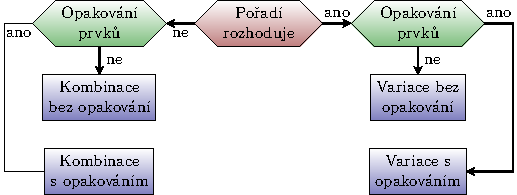
\includegraphics[width=0.7\linewidth]{mai_fig021.pdf}
        \caption{Typy výběrů. \cite[s.~201]{Musilova2009MA1}}
        \label{mai:fig021}
      \end{figure}

      Představuje-li daný výběr například volejbalové družstvo osmi děvčat (šest hráček a dvě 
      náhradnice), které bude reprezentovat v soutěži třídu osmou bé, do níž chodí \num{25} děvčat 
      a \num{18} chlapců, jedná se o výběr \(k - 8\) prvků z počtu \(n = 25\) prvků. Chlapce nelze 
      postavit do družstva volejbalistek. Každý výběr možného družstva bude představovat 
      \emph{kombinaci bez opakování}, neboť pořadí hráček nehraje roli a třeba Aničku Novákovou 
      máme ve třídě jen jednu. Budeme-li však chtít vytvářet z deseti cifer \(0, 1, \ldots, 9\) 
      trojciferná čísla, pak tyto výběry tří prvků z deseti (\(k = 3\), \(n = 10\)) jsou 
      \emph{variacemi s opakováním}. Čísla \num{125}, \num{512}, \num{251}, \num{215}, \num{521} a 
      \num{152} jsou totiž různá, a například \num{222} je také trojciferné číslo. Kombinace s 
      opakováním bychom mohli vytvářet třeba i při výběru různobarevných ponožek ze zásuvky a 
      konečně \emph{variacemi bez opakování} by mohly být dejme tomu trojbarevné signály (\(k = 
      3\)) tvořené trojicemi barevných hadříků vybíraných z \(n\) barev (pro \(n = 3\) třeba zrovna 
      z těch ponožek). Nyní bychom však rádi věděli, jak pro zadané hodnoty \(n\) a \(k\) určit 
      počet všech možných výběrů předepsaného typu. Ukážeme si to na příkladech.

      %--Šance milion-------------------------------------------------
      % !TeX spellcheck = cs_CZ
\begin{mdframed}[style=mdexam]
  \begin{example}\label{mai:exam007}
    \textbf{Šance milion}:\newline
    „Znáte nějakou jinou hru, kde můžete denně vyhrát milion?“ Tento nebo jiný, obdobně nepříliš
    vtipný reklamní slogan propaguje v televizi hru, jejímž cílem je uhodnout šestici tažených cifer
    ve správném pořadí. (Hru raději nehrajte, pravděpodobnost výhry je mizivá.) Tah se provádí
    následovně: V každém ze šesti bubnů, očíslovaných pořadovými čísly \num{1} až \num{6}, je
    připraveno deset míčků opatřených ciframi \(0, 1, \ldots, 9\). Z prvního bubnu se náhodně
    vylosuje jedna cifra (deset možností). Poté se náhodně vylosuje jedna cifra z druhého bubnu
    (opět deset možností). Možností vzniku uspořádané dvojice cifer (jedna cifra z prvního a druhá z
    druhého bubnu) je již sto (každou možnost výsledku u prvního bubnu lze kombinovat s každou
    možností výsledku z druhého bubnu). Losování pokračuje u třetího, čtvrtého, pátého a šestého
    bubnu. Celkový počet možností je \num{1e6}, tedy \textbf{milion}. (Šance získat výhru, tedy
    vyhrát milion, je ovšem pouze jedna milióntina, neboť z milionu možností je pouze jedna skutečně
    tažena.) 
  \end{example}
\end{mdframed}
      %---------------------------------------------------------------
      
      Zobecněním předchozího příkladu získáváme vzorec pro počet \textbf{variací s opakováním} 
      \emph{k}-té třídy z \(n\) prvků. Při tahu totiž záleží na pořadí bubnů a každý buben obsahuje 
      všechny cifry. Výsledky tahů z jednotlivých bubnů se tedy mohou opakovat. Pokud by bubnů bylo 
      \(k\) a v každém \(n\) různých cifer, dostali bychom pro \textbf{variace s opakováním 
      \(k\)-té třídy z \(n\) prvků} celkový počet
      \begin{equation}\label{mai:eq007}
        \boxed{V_k' = n^k}\, .
      \end{equation}

      %--Modifikovaná šance milion------------------------------------
      % !TeX spellcheck = cs_CZ
\begin{example}\label{mai:exam008}
  \textbf{Modifikovaná šance milion}:\newline
  Představme si hru z předchozího příkladu upravenou takto: K dispozici bude jen jeden buben s 
  ciframi \(0, 1, \ldots, 9\), každá cifra je v bubnu obsažena pouze jednou. Opět máme losovat 
  uspořádanou \textbf{šestici cifer}. Nyní se však jedná o \textbf{variace šesté třídy z deseti 
  prvků bez opakování}. S jediným bubnem musíme totiž provést šest losování, přičemž při každém 
  losování ubude z bubnu jedna cifra. Při prvním tahu je deset možností, při druhém již jen devět, 
  atd., při šestém již pouze pět možností. Celkem je tedy \(10 \cdot 9 \cdots 5 = \num{151200}\) 
  možností.
\end{example}
      %---------------------------------------------------------------
      
      Uvážíme-li, že v předchozím příkladu je \(n = 10\) a \(k = 6\), dostáváme pro \textbf{počet 
      variací bez opakování \(k\)-té třídy z \(n\) prvků} obecný vztah
      \begin{align}
        V_k(n) &= n(n-1)(n-2)\cdots(n-k+1)  \nonumber \\
        \shortintertext{neboli}
        V_k(n) &= \frac{n!}{(n-k)!}\, .    \label{mai:eq008}
      \end{align}
      Poznamenejme, že \(n!\) značí \textbf{faktoriál}, \(n! = n(n - 1)\cdots 3 \cdot 2 \cdot 1\). 
      Pro nulu definujeme \(0! = 1\). Je zřejmé, že při vytváření variací bez opakování musí být 
      \(k\leqq n\). Variace bez opakování \(n\)-té třídy z \(n\) prvků se nazývají 
      \textbf{permutace}. Každá z nich představuje určité uspořádání těchto \(n\) prvků. Platí
      \begin{equation}\label{mai:eq009}
        \boxed{P(n) = V_n(n) = n!}\, .
      \end{equation}
      
      Nyní odvodíme vzorec pro počet \textbf{kombinací \(k\)-té třídy z \(n\) prvků bez opakování}. 
      Již jsme si řekli, že \emph{kombinací} rozumíme takový výběr z celkového počtu \(n\) prvků, 
      který obsahuje určitých \(k\) prvků nezávisle na jejich pořadí. Představme si, že máme k 
      dispozici všechny variace bez opakování \(k\)-té třídy ze zmíněných \(n\) prvků. Vezměme 
      kteroukoli z nich. Soubor všech variací \(k\)-té třídy z \(n\) prvků však obsahuje i další 
      variace, lišící se od té naší jen pořadím prvků. Celkem je takových variací (i s tou první) 
      \(k!\) a z hlediska kombinací představují totéž. Soubor variací se tak rozpadá na podsoubory, 
      z nichž každý obsahuje \(k!\) variací lišících se navzájem pouze pořadím prvků. Každý z 
      těchto podsouborů představuje však jedinou kombinaci. Počet kombinací \(k\)-té třídy z \(n\) 
      prvků bez opakování je tedy
      \begin{equation}\label{mai:eq010}
        \boxed{C(k) = \frac{V_k(n)}{P(k)} = \frac{n!}{(n-k)!\,k!} = 
               \begin{pmatrix}
                n \\
                k
               \end{pmatrix}}\, .
      \end{equation}
      
      Pro odvození vzorce pro \textbf{kombinace s opakováním} použijeme opět příkladu.
      %--Kuličky v přihrádkách----------------------------------------
      % !TeX spellcheck = cs_CZ
\begin{mathexam}{Kuličky v přihrádkách}{exam009}
  Máme kuličky \(n\) různých barev, v každé barvě máme tolik kuliček, kolik bude potřeba. Naším
  úkolem je vytvářet výběry \(k\) kuliček. Na \textbf{pořadí barev nezáleží}, kuliček jedné barvy
  může být ve výběru libovolný počet \(0\leqq s \leqq k\). Výběry budeme vytvářet tak, že budeme
  kuličky dávat do \(n\) přihrádek, z nichž každá bude vyhrazena pro určitou barvu. Pokud tedy v
  daném výběru zrovna nebude třeba modrá kulička, bude přihrádka vyhrazená pro modrou barvu prázdná.
  Budou-li v daném výběru právě tři červené kuličky, budou umístěny v přihrádce vyhrazené pro
  červenou barvu. Vidíme, že pokud konkrétním přihrádkám přisoudíme konkrétní barvy, samotné kuličky
  by již barevné být nemusely, stačily by třeba kuličky skleněné, bezbarvé. Zůstane-li například
  přihrádka pro modrou barvu prázdná, víme, že daný výběr neobsahuje modrou barvu. Budou-li v
  přihrádce pro červenou barvu tři (bezbarvé) kuličky, víme, že daný výběr obsahuje červenou barvu
  třikrát. Příklad takové situace ukazuje následující schéma:
  
  {\centering
    \luafigure[0.9]{mai_fig033.pdf}
    \par}

  Náš úkol můžeme přeformulovat takto: Je třeba rozmístit \(k\) kuliček do \(n\) přihrádek. V každé
  přihrádce může být obecně \(s\) kuliček, kde \(0\leqq s \leqq k\), přitom celkový počet kuliček
  musí být samozřejmě stále \(k\). Můžeme si představit, že \(k\) kuliček máme položených v řadě na
  polici mezi dvěma pevnými stěnami (krajní svislé čáry v předchozím schématu) a různé způsoby
  rozmístění kuliček do přihrádek provádíme přemísťováním pohyblivých přepážek. Kdybychom například
  v předchozím schématu přesunuli druhou svislou čáru, počítáno zleva, až za první kuličku v
  přihrádce na červenou barvu, dostaneme uspořádání, při němž je v přihrádce na modrou barvu jedna
  kulička a v přihrádce na červenou barvu dvě kuličky. Tedy takto:

  {\centering
    \luafigure[0.9]{mai_fig034.pdf}
  \par}

  Mezi dvěma krajními pevnými stěnami máme tedy k dispozici \(k\) pozic pro kuličky a \((n - 1)\)
  pozic pro pohyblivé přepážky. Celkem tedy \((n + k - 1)\) pozic, na které můžeme libovolně
  rozmísťovat \(k\) kuliček a \((n - 1)\) přepážek. Do těchto \((n + k - 1)\) pozic můžeme umístit
  \(k\) kuliček \(C_k'(n)\) způsoby, kde
  \begin{equation}\label{MAI:eq011}
    \boxed{C_k'(n) =  \binom{n + k - 1}{k} = \binom{n + k - 1}{n -1}}\, .
  \end{equation}
  Na zbylé pozice již musíme umístit přepážky. Nebo naopak, nejprve umístíme \((n - 1)\) přepážek a
  potom kuličky. Výsledek je stejný, jak je vidět z předchozího vzorce. Protože jsme vytváření
  kombinací s opakováním \(k\)-té třídy z \(n\) prvků převedli na úlohu o rozmísťování kuliček do
  přihrádek, udává získaný vzorec právě počet takových kombinací. Aby měl vzorec smysl, musí platit
  \(n + k - 1 \geqq k\), tedy \(n \geqq 1\).

  Komu nevyhovuje představa kuliček v přihrádkách a má raději čísla, může uvažovat následovně: Tak
  jako je každé číslo v desítkové soustavě zapsáno pomocí cifer \(0, 1, 2, \ldots , 8, 9\), je k
  jeho zápisu ve dvojkové soustavě potřeba pouze dvou cifer, nuly a jedničky. Představme si nyní
  přepážku jako jedničku a kuličku jako nulu. Náš úkol zjistit počet všech možných způsobů rozdělení
  \(k\) kuliček do \(n\) přihrádek, ohraničených \((n+1)\) přepážkami, můžeme převést na
  ekvivalentní problém: Kolik dokážeme najít čísel, která jsou ve dvojkové soustavě zapsána právě
  \(k\) nulami a \((n + 1)\) jedničkami, požadujeme-li, aby první i poslední cifrou byla jednička?
  Odpověď je jednoduchá. Máme k dispozici \((n+k+1)\) pozic pro cifry. První a poslední pozice jsou
  pevně obsazeny jedničkami, volných pozic je tedy pouze \((n + k - 1)\). Počet všech různých
  způsobů, kterými na \(k\) z těchto pozic můžeme umístit nuly, je roven počtu kombinací \(k\)-té
  třídy z \((n + k - 1)\) prvků. Na zbylé pozice již musíme umístit jedničky. Komplementárně,
  budeme-li hledat počet všech možných způsobů, jak na \((n-1)\) pozic umístit jedničky, dostaneme
  shodný výsledek, v souhlasu se vzorcem (\ref{mai:eq010}).
\end{mathexam}
      %---------------------------------------------------------------
      
      %--Obsazování kvantových stavů----------------------------------
      % !TeX spellcheck = cs_CZ
\begin{example}\label{mai:exam010}
  \textbf{Obsazování kvantových stavů}:\newline\small
  Úloha o kuličkách a přihrádkách má přímou aplikaci v \textbf{kvantové fyzice}. Představme si, že 
  fyzikální soustava je tvořena \(k\) částicemi. Každá částice se nachází v určitém stavu, v němž 
  jí můžeme přisoudit fyzikální charakteristiky, které jsou s tímto stavem spojeny (třeba energii, 
  moment hybnosti, apod.). Jednotlivé stavy jsou pak rozlišitelné právě pomocí těchto 
  charakteristik. Dejme tomu, že přípustných stavů je \(n \geqq 1\). Problémem kvantové fyziky je 
  to, že kvantové částice jsou nerozlišitelné. Nepoznáme jednu od druhé. Je to stejné, jako bychom 
  měli \(k\) naprosto stejně vypadajících kuliček, které nemáme nijak očíslovány. Záměna dvou 
  částic (nerozlišitelných kuliček) se nepozná, nevede tedy ke změně stavu fyzikální soustavy. Pro 
  hodnoty fyzikálních charakteristik soustavy jako celku je tedy důležité jen to, kolik částic je v 
  každém z přípustných stavů. Musíme se tedy zajímat o to, kolika způsoby lze našich \(k\) 
  \textbf{nerozlišitelných částic} (kuliček) umístit do \(n\) \textbf{stavů} (přihrádek). Kvantové 
  částice jsou však dvojího druhu, \textbf{fermiony} (například elektrony, neutrony, protony, jádra 
  s lichým počtem nukleonů) a \textbf{bosony} (například fotony, mezony, jádra se sudým počtem 
  nukleonů). Rozdíl mezi nimi je ten, že bosony se „dobře snášejí“, a proto jich může být v jednom 
  stavu i více. 
  \begin{itemize}\addtolength{\itemsep}{-0.5\baselineskip}
    \item Počet možností, jak rozmístit \(k\) \textbf{bosonů} po \(n\) stavech je tedy
          \begin{equation*}
            N_{\text{boson}} = 
              \begin{pmatrix}
                n + k - 1 \\
                    k
               \end{pmatrix}
          \end{equation*}
    \item S \textbf{fermiony} je tomu jinak. \textbf{Pauliho vylučovací princip} jim zakazuje, 
          aby v daném stavu byl více než jeden fermion. Stav může být buď prázdný, nebo obsazen 
          jedním fermionem. V takovém případě musí být \(n \geqq k\) a v každé přihrádce může být 
          nejvýše jedna kulička. Situace tak odpovídá \textbf{kombinacím bez opakování \(k\)-té 
          třídy z \(n\) prvků}, tj.
          \begin{equation*}
            N_{\text{fermion}} = 
              \begin{pmatrix}
                n  \\
                k
              \end{pmatrix}
          \end{equation*}
  \end{itemize}
\normalsize
\end{example}
      %---------------------------------------------------------------
      
      Získané kombinatorické vzorce nyní použijeme při řešení základních úloh o pravděpodobnostech. 
      V každé úloze bude důležité
      \begin{itemize}
        \item definovat jev \(A\), jehož pravděpodobnost počítáme,
        \item určit počet \(N\) případů možných, tj. počet všech možných výsledků pokusu, při 
              kterém sledujeme, zda jev \(A\) nastal či nenastal,
        \item určit počet \(M\) případů příznivých, tj. počet těch výsledků daného pokusu, při 
              kterých jev \(A\) nastal.
      \end{itemize}

      %--Výhra ve sportce---	----------------------------------------
      % !TeX spellcheck = cs_CZ
\wikitextrule
\begin{example}\label{mai:exam052}
  \textbf{Výhra ve sportce}\newline\small
  Jaká je pravděpodobnost hlavní výhry ve sportce? Všichni víme, že malá, ale máme představu, jak 
  malé toto číslo je? Při sportce se losuje \(k = 6\) čísel a jedno dodatkové z celkového počtu \(n 
  = 49\) čísel. (Dříve byla čísla spojena s názvy sportů, odtud název „sportka“ .) Na pořadí čísel 
  ve výběru nezáleží, vytažené číslo se do hry nevrací. Jde tedy o \textbf{kombinace bez 
  opakování}. Hlavní výhra požaduje uhodnout všech \num{6} tažených čísel. Jev \(A\) je tedy 
  definován takto:
  
  \begin{itemize}
    \item Jev \(A\): Bude taženo právě oněch \num{6} čísel, která jsem vsadil.
          Počet možností, které při tahu sportky mohou nastat (počet případů možných), je \(N = 
          \begin{pmatrix} n \\ k\end{pmatrix} =  \begin{pmatrix} 49 \\ 6 \end{pmatrix} \). Hlavní 
          výhru představuje jediná kombinace, počet příznivých případů je proto \(M = 1\). 
          Pravděpodobnost hlavní výhry ve sportce, tj. pravděpodobnost jevu \(A\), je
          \begin{equation*}
            p(A) = \dfrac{M}{N} = \dfrac{1}{\begin{pmatrix} 49 \\ 6 \end{pmatrix}} 
                 = \dfrac{43!6!}{49!} = \dfrac{720}{49\cdot48\cdot47\cdot46\cdot45\cdot44} \simeq 
                 \num{7e-8}
                 = \SI{7e-6}{\percent}
          \end{equation*}
          Pravděpodobnost hlavní výhry je velmi malá, sedm milióntin procenta. 
    \item A o kolik lepší to bude s pravděpodobností některé z vedlejších výher? Tak třeba pátá 
          cena znamená, že je nutné ze šesti tažených čísel uhodnout libovolné tři. Jev \(A\) je 
          tedy: Ze šesti čísel, která jsme vsadili, budou v tažené kombinaci obsažena právě tři 
          libovolná z nich. Počet \(N\) zůstává stejný jako v předchozí části úlohy. Je třeba jen 
          určit \(M\). Každý příznivý případ vzniká tak, že trojice správných čísel (výběry tří ze 
          šesti) je doplněna trojicí chybných čísel (výběry tří ze čtyřiceti tří). Tedy \(M = 
          \begin{pmatrix}6 \\ 3\end{pmatrix}\begin{pmatrix} 49 - 6 \\ 3\end{pmatrix} =  
          \begin{pmatrix} 6 \\ 3\end{pmatrix}\begin{pmatrix} 43 \\ 3 \end{pmatrix}\),
          \begin{align*}
            p(A) &= \dfrac{M}{N} 
                  = \dfrac{\begin{pmatrix} 6 \\ 3\end{pmatrix}
                           \begin{pmatrix} 43 \\ 3 \end{pmatrix}}
                          {\begin{pmatrix} 49 \\ 6\end{pmatrix} }                
                  =\left(\dfrac{6!}{3!\cdot3!}\right)\left(\dfrac{43!}{40!\cdot3!}\right)
                   \left(\dfrac{43!6!}{49!}\right)                                            \\
                 &=\dfrac{120\cdot43\cdot42\cdot41\cdot720}
                         {49\cdot48\cdot47\cdot46\cdot45\cdot44\cdot36} 
                  \simeq\num{0.018}.
          \end{align*}
          Tato pravděpodobnost již zanedbatelná není, na rozdíl od finanční částky, jíž bývá 
          ohodnocena pátá cena. Sázení sportky může domácímu rozpočtu spíše ublížit.
    \item Třetí, resp. čtvrtá cena jsou, podobně jako první a pátá, definovány velmi jednoduše. Je 
          třeba uhodnout pět, resp. čtyři ze šesti tažených čísel. V případě druhé ceny hraje roli
          dodatkové číslo. Druhou cenu získává ten, kdo uhodl pět ze šesti čísel vylosovaných v 
          prvním tahu a ještě navíc číslo dodatkové, které se losuje ze zbylých \num{43} čísel, jež 
          zůstala po prvním tahu v osudí. Jev \(A\) je tedy definován takto:
          
          Ze šesti čísel, která jsem vsadil, bude při prvním tahu vylosováno libovolných pět a v 
          druhém tahu bude vylosováno právě to dodatkové číslo, které jsem vsadil. Počet případů 
          příznivých je pouze \(M = \begin{pmatrix}6 \\ 5\end{pmatrix}\), neboť šestým číslem 
          nemůže být libovolné ze \num{43} čísel, která nebyla v prvním tahu vylosována, ale 
          musí to být právě číslo dodatkové. Pravděpodobnost jevu \(A\) je
          \begin{equation*}
            p(A)  = \dfrac{M}{N} 
                  = \dfrac{\begin{pmatrix} 6  \\ 5\end{pmatrix}}
                          {\begin{pmatrix} 49 \\ 6\end{pmatrix}}
                  \simeq\num{4.2e-17}.
          \end{equation*}
          
          Pokud bychom jako jev \(A\) označili výhru jakékoliv ceny, dostaneme
          \begin{align*}
            M &= \sum_{6}^{k=3}\begin{pmatrix} 6  \\   k  \end{pmatrix}
                               \begin{pmatrix} 43 \\ 6 - k\end{pmatrix}  +
                               \begin{pmatrix} 6  \\   5  \end{pmatrix}                      \\
              &= \begin{pmatrix} 6 \\ 3\end{pmatrix}\begin{pmatrix} 43 \\ 3\end{pmatrix} +
                 \begin{pmatrix} 6 \\ 4\end{pmatrix}\begin{pmatrix} 43 \\ 2\end{pmatrix} +
                 \begin{pmatrix} 6 \\ 5\end{pmatrix}\begin{pmatrix} 43 \\ 1\end{pmatrix} +
                 \begin{pmatrix} 6 \\ 6\end{pmatrix}\begin{pmatrix} 43 \\ 0\end{pmatrix} +
                 \begin{pmatrix} 6 \\ 5\end{pmatrix},                                        \\
           p(A) &= \dfrac{\begin{pmatrix}  6 \\ 3\end{pmatrix}
                          \begin{pmatrix} 43 \\ 3\end{pmatrix}  +
                          \begin{pmatrix}  6 \\ 4\end{pmatrix}
                          \begin{pmatrix} 43 \\ 2\end{pmatrix}  +
                          \begin{pmatrix}  6 \\ 5\end{pmatrix}
                          \begin{pmatrix} 43 \\ 1\end{pmatrix}  +
                          \begin{pmatrix}  6 \\ 6\end{pmatrix}
                          \begin{pmatrix} 43 \\ 0\end{pmatrix}  +
                          \begin{pmatrix}  6 \\ 5\end{pmatrix}}
                         {\begin{pmatrix} 49 \\ 6\end{pmatrix}} =\simeq\num{0.019}.
          \end{align*}
          Všimněte si, že tento výsledek je roven součtu pravděpodobností výhry páté, čtvrté, 
          třetí, druhé a hlavní ceny. Později si tento závěr ještě připomeneme.
  \end{itemize}  
  \normalsize
\end{example}
      %---------------------------------------------------------------

      %--Losování karet-----------------------------------------------
      % !TeX spellcheck = cs_CZ
\wikitextrule
\begin{example}\label{mai:exam053}
  \textbf{Losování karet}\newline\small
    Máme karetní hru mariáš, která obsahuje celkem \num{32} karet osmi hodnot \num{7}, \num{8}, 
    \num{9}, \num{10}, J (kluk), Q (dáma), K (král), A (eso), každá hodnota je ve čtyřech barvách, 
    červené barvy jsou \(\heartsuit\) (srdce) a \(\lozenge\) (kára), černé barvy jsou \(\spadesuit\)
    (piky) a \(\clubsuit\) (kříže). Jaká je pravděpodobnost, že při náhodném vylosování deseti 
    karet budou 
    mezi nimi:
    \begin{enumerate}[label=\Alph*]
      \item právě dvě esa,
      \item alespoň dvě esa,
      \item nejvýše dvě esa,
      \item alespoň šest karet stejné barvy,
      \item právě dvě dámy a alespoň jeden kluk,
      \item právě dvě dámy nebo alespoň jeden kluk?
    \end{enumerate}

    Písmena (A) až (F) představují různé části úlohy a také zároveň definují jevy, jejichž 
    pravděpodobnost počítáme. Jedná se opět o kombinace. Nezáleží totiž na pořadí, v jakém karty 
    vytahujeme. Důležité je jen to, zda jsou vyjmenované karty ve výběru obsaženy. Počet možných 
    výsledků náhodného vylosování deseti karet z dvaatřiceti, tj. počet případů možných, je pro 
    všechny části úlohy stejný,
    \begin{equation*}
      N = \begin{pmatrix} 32 \\ 10\end{pmatrix} 
        = \dfrac{32\cdot31\cdots24\cdot23}{10\cdot9\cdots2\cdot1} = \num{64512240}.
    \end{equation*}
    
    Počítejme nyní případy příznivé pro jednotlivé jevy \(A\) až \(F\) a pravděpodobnosti těchto 
    jevů:
    \begin{equation*}
      M(A) = \begin{pmatrix} 4 \\ 2\end{pmatrix}\begin{pmatrix} 32 - 4 \\ 10 - 2\end{pmatrix}
           = \begin{pmatrix} 4 \\ 2\end{pmatrix}\begin{pmatrix} 28 \\ 8\end{pmatrix}
           = 6\cdot\dfrac{28\cdot27\cdots1}{8\cdot7\cdots2\cdot1} = \num{18648630}.
    \end{equation*}
    Jak jsme k tomuto výsledku došli? Příznivý pro daný jev je každý výběr, v němž jsou obsažena 
    právě dvě esa (libovolných barev) a žádná další esa (význam slova „právě“). Počet výběrů dvou 
    es z celkového počtu čtyř es je \(C_2(4)\), počet výběrů dalších libovolných osmi karet ze 
    zbývající části hry, která vznikne po odstranění es (nechceme, aby v příznivém výběru byla 
    další esa), je \(C_{(10-2)}(32 - 4) = C_8(28)\). Každý výběr dvojice es lze kombinovat s každým 
    výběrem zbývajících osmi karet ze zbytku hry, tj. \(M(A) = C_2(4)\cdot C_8(28)\). A to je právě
    náš předchozí výsledek. Potom:
    \begin{equation*}
      p(A) = \dfrac{M(A)}{N} 
           = \dfrac{\begin{pmatrix} 4 \\ 2\end{pmatrix}\begin{pmatrix} 28 \\ 8\end{pmatrix}}
                   {\begin{pmatrix} 32 \\ 10\end{pmatrix}}
           = \dfrac{\num{18648630}}{\num{64512240}} \simeq \num{0.29}
    \end{equation*}
    
    Aby nastal jev \(B\), požadujeme, aby v náhodném výběru deseti karet z dvaatřiceti byla alespoň 
    dvě esa. To znamená, že výběr považujeme za příznivý, obsahuje-li dvě esa libovolné barvy a osm 
    libovolných karet jiné hodnoty, nebo obsahuje tři esa libovolné barvy a sedm libovolných karet 
    jiné hodnoty, nebo obsahuje všechna čtyři esa a šest libovolných karet jiné hodnoty, \(k\) es 
    (pro \(k = 2, 3, 4\)) můžeme ze čtyř es vybrat \(\begin{pmatrix} 4 \\ k\end{pmatrix}\) způsoby.
    \(10 - k\) karet jiné hodnoty pak musíme vybírat pouze z \num{28} karet (esa je nutno 
    odstranit, aby bylo zaručeno, že „doplňkové“ karty budou mít jinou hodnotu než eso). Výběr 
    zbývajících karet lze učinit \(\begin{pmatrix} 28 \\ 10 - k\end{pmatrix}\) způsoby. Nakonec 
    tedy dostáváme
    \begin{align*}
      M(B) &=  \begin{pmatrix} 4 \\ 2\end{pmatrix}\begin{pmatrix} 28 \\ 8\end{pmatrix}
              +\begin{pmatrix} 4 \\ 3\end{pmatrix}\begin{pmatrix} 28 \\ 7\end{pmatrix}
              +\begin{pmatrix} 4 \\ 4\end{pmatrix}\begin{pmatrix} 28 \\ 6\end{pmatrix}         \\
           &=  6\cdot\dfrac{28\cdot27\cdots22\cdot21}{8\cdot7\cdots2\cdot1}
              +4\cdot\dfrac{28\cdot27\cdots23\cdot22}{7\cdot6\cdots2\cdot1}
              +1\cdot\dfrac{28\cdot27\cdots24\cdot23}{6\cdot5\cdots2\cdot1} = \num{23761530},  \\
      P(B) &= \dfrac{M(B)}{N} = \dfrac{\num{23761530}}{\num{64512240}} \simeq\num{0.37}.
    \end{align*}
    Pozn.: Někomu se předchozí výpočet může zdát příliš složitý. Nelze jej nějak zjednodušit? Co 
    kdybychom uvažovali třeba takto: Výběr dvou es již zajistí splnění požadavku. Doplňkové karty 
    tedy již pak můžeme vybírat ze třiceti karet - nebudeme tedy odstraňovat esa, protože budou-li 
    vybrána mezi doplňkovými kartami, požadavek „alespoň dvou es ve výběru“ to nenaruší. Při takové 
    interpretaci bychom dostali
    \begin{equation*}
      M(B) = \begin{pmatrix} 4 \\ 2\end{pmatrix}\begin{pmatrix} 30 \\ 8\end{pmatrix}   
           = 6\cdot\dfrac{30\cdot29\cdots24\cdot23}{8\cdot7\cdots2\cdot1}
           = \num{35117550}.
    \end{equation*}
    Vidíme, že vyšlo číslo vyšší než při předchozí úvaze. Co je tedy správně? Správně je první 
    úvaha vedoucí k nižšímu počtu příznivých případů. Při druhé úvaze jsme některé případy 
    započetli vícekrát. Zkuste přijít na to, jak se to stalo. V každém případě vidíme, že 
    kombinatorické úvahy, ať již vypadají jakkoli jednoduše, mohou být zrádné a je třeba dát si na 
    ně pozor. 
    
    Jev \(C\) podle zadání nastane, obsahuje-li náhodný výběr deseti karet nejvýše dvě esa. Znamená 
    to, že výběr je příznivý, neobsahuje-li žádné eso a obsahuje deset karet jiné hodnoty, nebo 
    obsahuje-li jedno eso a devět karet jiné hodnoty, nebo obsahuje-li dvě esa a osm karet jiné 
    hodnoty. Počet \(M(C)\) určíme analogicky jako \(M(B)\), ale pro \(k= 0, 1, 2\):
    \begin{align*}
      M(C) &=  \begin{pmatrix} 4 \\ 0\end{pmatrix}\begin{pmatrix} 28 \\ 10\end{pmatrix}
              +\begin{pmatrix} 4 \\ 1\end{pmatrix}\begin{pmatrix} 28 \\ 9\end{pmatrix}
              +\begin{pmatrix} 4 \\ 2\end{pmatrix}\begin{pmatrix} 28 \\ 8\end{pmatrix}         \\
           &=   \cdot\dfrac{28\cdot27\cdots20\cdot19}{10\cdot9\cdots2\cdot1}
              +4\cdot\dfrac{28\cdot27\cdots21\cdot20}{ 9\cdot8\cdots2\cdot1}
              +6\cdot\dfrac{28\cdot27\cdots22\cdot21}{ 8\cdot7\cdots2\cdot1} = \num{59399340}, \\
      P(C) &= \dfrac{M(C)}{N} = \dfrac{\num{59399340}}{\num{64512240}} \simeq\num{0.92}.
    \end{align*}
    
    Jev \(D\) znamená alespoň šest karet stejné barvy (připomeňme, že barvou rozumíme jednu z 
    možností \(\heartsuit\), \(\lozenge\), \(\spadesuit\), \(\clubsuit\)). Hra obsahuje osm karet 
    od každé barvy. Současně je tedy zřejmé, že karet stejné barvy může být ve výběru nejvýše osm. 
    Výběr je příznivý pro \(k = 6, 7, 8\). Obdobnou úvahou jako v předchozích případech dostáváme
    \begin{equation*}
      M = 4\cdot\sum^{8}_{k=6}
          \begin{pmatrix} 8 \\ k \end{pmatrix}\begin{pmatrix} 32 - 8 \\ 10 - k\end{pmatrix}
        = \num{1255984}.
    \end{equation*}
    
    Faktor \num{4} před celou sumou se objevuje proto, že nebylo specifikováno, která ze čtyř barev 
    má být zastoupena alespoň šesti kartami. Všechny čtyři možnosti volby barvy jsou tedy příznivé. 
    Pravděpodobnost jevu \(D\) je
    \begin{equation*}
      p(D)  = \dfrac{M(D)}{N}
            = \dfrac{4\cdot\sum^{8}_{k=6}\dfrac{8!}{k!(8-k)!}\dfrac{24!}{(10-k)!(14+k)!}}
                    {\begin{pmatrix} 32 \\ 10 \end{pmatrix}}                               
            = \dfrac{\num{1255984}}{\num{64512240}} \simeq \num{0.019}.
    \end{equation*}
    
    Případy (\(E\)) a (\(F\)) v zadání se liší pouze slůvkem „a“ a „nebo“. Uvidíme, že nejde o 
    slovíčka, ale o podstatný rozdíl. 
    
    Aby nastal jev \(E\), požadujeme, aby náhodný výběr deseti karet obsahoval právě dvě dámy a 
    alespoň jednoho kluka. Znamená to, že výběr je příznivý, obsahuje-li dvě dámy libovolné barvy a 
    současně alespoň jednoho kluka libovolné barvy. Příznivé možnosti tedy jsou:
    \begin{enumerate}
    \item  dvě dámy libovolné barvy, jeden kluk libovolné barvy, \num{7} libovolných karet, které 
           nemají hodnotu dámy ani kluka, celkem 
           \(\begin{pmatrix} 4 \\ 2 \end{pmatrix}
             \begin{pmatrix} 4 \\ 1\end{pmatrix}
             \begin{pmatrix} 32-2\cdot4 \\ 7 \end{pmatrix} = \num{8306496}\) možností,
    \item dvě dámy libovolné barvy, dva kluci libovolné barvy, \num{6} libovolných karet, které 
          nemají hodnotu dámy ani kluka, celkem 
          \(\begin{pmatrix} 4 \\ 2 \end{pmatrix}
            \begin{pmatrix} 4 \\ 2\end{pmatrix}
            \begin{pmatrix} 32-2\cdot4 \\ 6 \end{pmatrix} = \num{4845456}\) možností,
    \item dvě dámy libovolné barvy, tři kluci libovolné barvy, \num{5} libovolných karet, které 
          nemají hodnotu dámy ani kluka, celkem 
          \(\begin{pmatrix} 4 \\ 2 \end{pmatrix}
            \begin{pmatrix} 4 \\ 3\end{pmatrix}
            \begin{pmatrix} 32-2\cdot4 \\ 5 \end{pmatrix} = \num{1020096}\) možností,
    \item dvě dámy libovolné barvy, všichni čtyři kluci, \num{4} libovolné karty, které nemají 
          hodnotu dámy ani kluka, celkem 
          \(\begin{pmatrix} 4 \\ 2 \end{pmatrix}
            \begin{pmatrix} 4 \\ 4\end{pmatrix}
            \begin{pmatrix} 32-2\cdot4 \\ 4 \end{pmatrix} = \num{63756}\) možností.
    \end{enumerate}
    \begin{align*}
      M(E) &= \begin{pmatrix} 4 \\ 2 \end{pmatrix}\cdot\sum^{4}_{k=1}
              \begin{pmatrix} 4 \\ k \end{pmatrix}\begin{pmatrix} 24 \\ 8 - k \end{pmatrix}
            = 6\left[ 
                  4\begin{pmatrix} 24 \\ 7 \end{pmatrix} +
                  6\begin{pmatrix} 24 \\ 6 \end{pmatrix} +
                  4\begin{pmatrix} 24 \\ 5 \end{pmatrix} +
                   \begin{pmatrix} 24 \\ 4 \end{pmatrix}
                \right]                                                      \\ 
      M(E) &= \num{14235804},                                                \\
      p(E) &= \dfrac{M(E)}{N} = \dfrac{\num{14235804}}{\num{64512240}} \simeq \num{0.22}.
    \end{align*}
    
    Aby nastal jev \(F\), požadujeme, aby náhodný výběr deseti karet obsahoval právě dvě dámy nebo 
    alespoň jednoho kluka. Znamená to, že výběr je příznivý, obsahuje-li dvě dámy libovolné barvy a 
    jakékoli další karty, nebo obsahuje alespoň jednoho kluka a jakékoli další karty. Nyní je nutno 
    o všech možnostech pečlivě rozvažovat, abychom některé nezapočítali vícekrát. Pozor, slůvko 
    \uv{nebo} zde nemá vylučovací význam, připouští se, že mohou být splněny obě podmínky jevu 
    \(F\), tj. jak právě dvě dámy, tak alespoň jeden kluk. Příznivé možnosti jsou
    \begin{enumerate}
      \item dvě dámy libovolné barvy, žádný kluk, \num{8} libovolných karet, které nemají 
            hodnotu dámy ani kluka, celkem
            \begin{equation*}
              \begin{pmatrix} 4  \\ 2 \end{pmatrix}
              \begin{pmatrix} 4  \\ 0 \end{pmatrix}
              \begin{pmatrix} 32 - 2\cdot4 \\ 8 \end{pmatrix} = 6
              \begin{pmatrix} 24 \\ 8 \end{pmatrix},
            \end{equation*}
      \item žádná dáma, \(k\) kluků libovolné barvy pro \(k = 1, 2, 3, 4\) (alespoň jeden kluk), 
            \(10 - k\) karet, které nemají hodnotu dám y ani kluka, celkem
            \begin{equation*}
              \begin{pmatrix} 4  \\ 0 \end{pmatrix}
              \sum^{4}_{k=1}\begin{pmatrix} 4  \\ k \end{pmatrix}
                            \begin{pmatrix} 32 - 2\cdot4 \\ 10 - k \end{pmatrix} =
              \sum^{4}_{k=1}\begin{pmatrix} 4  \\ k \end{pmatrix}
                            \begin{pmatrix} 24 \\ 10 - k \end{pmatrix},
            \end{equation*}
      \item jedna dáma libovolné barvy, \(k\) kluků libovolné barvy pro \(k = 1,2, 3, 4\) (alespoň 
            jeden kluk), \(10 - k - 1\) karet, které nemají hodnotu dámy ani kluka, celkem
            \begin{equation*}
              \begin{pmatrix} 4  \\ 1 \end{pmatrix}
              \sum^{4}_{k=1}\begin{pmatrix} 4  \\ k \end{pmatrix}
                            \begin{pmatrix} 32 - 2\cdot4 \\ 10 - k - 1 \end{pmatrix} =
              4\sum^{4}_{k=1}\begin{pmatrix} 4  \\ k \end{pmatrix}
                            \begin{pmatrix} 24 \\ 9 - k \end{pmatrix},
            \end{equation*}
      \item dvě dámy libovolné barvy, \(k\) kluků libovolné barvy pro \(k = 1, 2, 3, 4\) (alespoň 
            jeden kluk), \(10 - 2 - k = 8 - k\) karet, které nemají hodnotu dámy ani kluka, celkem
            \begin{equation*}
              \begin{pmatrix} 4  \\ 2 \end{pmatrix}
              \sum^{4}_{k=1}\begin{pmatrix} 4  \\ k \end{pmatrix}
                            \begin{pmatrix} 32 - 2\cdot4 \\ 10 - k - 2 \end{pmatrix} =
              6\sum^{4}_{k=1}\begin{pmatrix} 4  \\ k \end{pmatrix}
                            \begin{pmatrix} 24 \\ 8 - k \end{pmatrix},
            \end{equation*}
      \item tři dámy libovolné barvy, k kluků libovolné barvy pro \(k = 1, 2, 3, 4\) (alespoň jeden 
            kluk), \(10 - k - 3\) karet, které nemají hodnotu dámy ani kluka, celkem
            \begin{equation*}
              \begin{pmatrix} 4  \\ 3 \end{pmatrix}
              \sum^{4}_{k=1}\begin{pmatrix} 4  \\ k \end{pmatrix}
                            \begin{pmatrix} 32 - 2\cdot4 \\ 10 - k - 3 \end{pmatrix} =
              4\sum^{4}_{k=1}\begin{pmatrix} 4  \\ k \end{pmatrix}
                            \begin{pmatrix} 24 \\ 7 - k \end{pmatrix},
            \end{equation*}
      \item všechny čtyři dámy, k kluků libovolné barvy pro \(k = 1, 2, 3, 4\) (alespoň jeden 
            kluk), \(10 - k - 4\) karet, které nemají hodnotu dámy ani kluka, celkem
            \begin{equation*}
              \begin{pmatrix} 4  \\ 4 \end{pmatrix}
              \sum^{4}_{k=1}\begin{pmatrix} 4  \\ k \end{pmatrix}
                            \begin{pmatrix} 32 - 2\cdot4 \\ 10 - k - 4 \end{pmatrix} =
              \sum^{4}_{k=1}\begin{pmatrix} 4  \\ k \end{pmatrix}
                            \begin{pmatrix} 24 \\ 6 - k \end{pmatrix},
            \end{equation*}
    \end{enumerate}
    
    Počet příznivých případů \(M(F)\) je dán součtem všech těchto možností, tedy
    \begin{equation*}
      M(F) = \begin{pmatrix}  4 \\ 2 \end{pmatrix}\begin{pmatrix} 4  \\ 0 \end{pmatrix}
             \begin{pmatrix} 24 \\ 8 \end{pmatrix} + 
              \sum^{4}_{s=0}\begin{pmatrix} 4  \\ s \end{pmatrix}
              \left[\sum^{4}_{k=1}\begin{pmatrix}  4 \\ k \end{pmatrix}
                    \begin{pmatrix} 24 \\ 10 - k - s \end{pmatrix}
              \right].
    \end{equation*}
    Všimněme si nyní výsledku. Výraz s dvojitou sumou můžeme přepsat jak
    \begin{equation*}
      \sum^{4}_{k=1}\begin{pmatrix} 4  \\ k \end{pmatrix}
        \left[\sum^{4}_{s=0}\begin{pmatrix}  4 \\ s \end{pmatrix}
              \begin{pmatrix} 24 \\ 10 - k - s \end{pmatrix}
        \right].
    \end{equation*}
    V učebnicích můžeme najít různé vzorce pro kombinační čísla, mezi nimi i vzorec
    \begin{equation*}
      \sum^{p}_{s=0}\begin{pmatrix} p \\ s \end{pmatrix}\begin{pmatrix} r \\ q - s \end{pmatrix}
        = \begin{pmatrix} r + p \\ q \end{pmatrix} \qquad\text{pro}\qquad r\geq q,\,q \geq p.
    \end{equation*}
    (Nebo si jej můžeme sami odvodit — pokuste se o to!) Pro \(p = 4\), \(r = 24\), \(q = 10 - k\), 
    \(1 \leq k \leq 4\) máme právě náš případ, takže
    \begin{equation*}
      \sum^{4}_{k=1}\begin{pmatrix} 4  \\ k \end{pmatrix}
        \left[\sum^{4}_{s=0}\begin{pmatrix}  4 \\ s \end{pmatrix}
              \begin{pmatrix} 24 \\ 10 - k - s \end{pmatrix}
        \right] = 
        \sum^{4}_{k=1}\begin{pmatrix}  4 \\ k \end{pmatrix}
                      \begin{pmatrix} 28 \\ 10 - k \end{pmatrix}.
    \end{equation*}
    Jak můžeme tento výsledek interpretovat? Jedná se o počet případů, kdy náhodný výběr deseti 
    karet z mariášové hry dvaatřiceti karet obsahuje alespoň jednu kartu pevně zvolené hodnoty (v 
    našem případě kluka), bez ohledu na to, kolik obsahuje karet ostatních hodnot. Přidáme-li počet 
    případů, kdy výběr neobsahuje žádného kluka a právě dvě dámy, dostaneme právě počet případů 
    příznivých pro jev \(F\). Pň úpravě použijeme ještě jednou vzorce
    \begin{equation*}
      \sum^{4}_{k=1}\begin{pmatrix} 4 \\ k \end{pmatrix}\begin{pmatrix} 28 \\ 10 - k\end{pmatrix}
        = \sum^{4}_{k=0}\begin{pmatrix}  4 \\ k     \end{pmatrix}
                        \begin{pmatrix} 28 \\ 10 - k\end{pmatrix} -
                        \begin{pmatrix}  4 \\ 0     \end{pmatrix}
                        \begin{pmatrix} 28 \\ 10    \end{pmatrix} =
                        \begin{pmatrix} 32 \\ 10    \end{pmatrix} -
                        \begin{pmatrix} 28 \\ 10    \end{pmatrix},
    \end{equation*}
    \begin{align*}
      M(F) &= \begin{pmatrix}  4 \\ 2 \end{pmatrix}\begin{pmatrix}  4 \\ 0 \end{pmatrix} 
              \begin{pmatrix} 24 \\ 8 \end{pmatrix} + 
              \sum^{4}_{k=1}\begin{pmatrix} 4  \\ k \end{pmatrix}
                      \left[\sum^{4}_{s=0}\begin{pmatrix}  4 \\ s \end{pmatrix}
                            \begin{pmatrix} 24 \\ 10 - k - s \end{pmatrix}
                      \right]                                                                   \\
           &= \begin{pmatrix}  4 \\ 2 \end{pmatrix}\begin{pmatrix} 24 \\ 8 \end{pmatrix} +
              \sum^{4}_{k=1}\begin{pmatrix}  4 \\ k \end{pmatrix}
                            \begin{pmatrix} 28 \\ 10 - k \end{pmatrix}                          \\
           &= \begin{pmatrix}  4 \\ 2 \end{pmatrix}\begin{pmatrix} 24 \\ 8 \end{pmatrix} + 
              \left[\begin{pmatrix}  32 \\ 10 \end{pmatrix} - 
                    \begin{pmatrix}  28 \\ 10 \end{pmatrix}
              \right]
            = \begin{pmatrix} 32 \\ 10 \end{pmatrix} - 
              \left[\begin{pmatrix} 28 \\ 10 \end{pmatrix} - 
                    \begin{pmatrix}  4 \\  2 \end{pmatrix}
                    \begin{pmatrix} 24 \\  8 \end{pmatrix}
              \right],                                                                          \\
      p(F) &= 1 - \dfrac{\begin{pmatrix} 28 \\ 10 \end{pmatrix} -
                         \begin{pmatrix}  4 \\  2 \end{pmatrix}
                         \begin{pmatrix} 24 \\  8 \end{pmatrix}
                        }
                        {\begin{pmatrix} 32 \\ 10 \end{pmatrix}}
            = 1 - \dfrac{\num{8710284}}{\num{64512240}} \simeq \num{0.86}.
    \end{align*}
    Zamysleme se ještě nad interpretací posledního výrazu pro \(M(F)\). Od počtu všech možných 
    případů se odečítá hodnota \(\begin{pmatrix} 28 \\ 10 \end{pmatrix}\) představující počet 
    situací, kdy ve výběru nebude žádný kluk, zmenšená o hodnotu \(\begin{pmatrix} 4 \\ 2 
    \end{pmatrix}\begin{pmatrix} 24 \\ 8 \end{pmatrix}\), která představuje počet situací, kdy ve 
    výběru budou právě dvě dámy a žádný kluk.
  \normalsize
\end{example}
      %---------------------------------------------------------------

      %--Sestavování čísel z cifer------------------------------------
      % !TeX spellcheck = cs_CZ
\wikitextrule
\begin{example}\label{mai:exam054}
  \textbf{Sestavování čísel z cifer}\newline\small
   Máme k dispozici libovolný počet cifer \(0, 1, \ldots, 9\). Kolik \(k\)-ciferných čísel z nich 
   můžeme sestavit? Odpověď na tuto otázku každý zná. Dvojciferná jsou čísla od \num{10} do 
   \num{99} včetně, je jich tedy \((99 - 10 + 1) = 90\). Trojciferná jsou od \(100\) do \(999\) 
   včetně, jejich počet je \((999 - 100 + 1) = 900\), \(k\)-ciferná jsou čísla od \(100\ldots0 = 
   1\cdot10^{k-1}\) do \(999\ldots9\) včetně (\(k\) devítek), jejich počet je \(9\cdot10^{k-1}\). 
   Tento výsledek bychom však měli získat i kombinatorickými úvahami. Čísla totiž dostáváme tak, že 
   z deseti cifer \(0, 1,\ldots, 9\) vytváříme variace \(k\)-té třídy s opakováním, musíme však 
   vyjmout ty možnosti, které začínají nulami. Dostáváme
   \begin{align*}
     10^k - 
       \left(
         9\cdot10^{k-2} + 9\cdot10^{k-3} + \cdots + 9\cdot10^1 + + 9\cdot10^0 + 1 
       \right)
        &= 10^k - 9\cdot\dfrac{10^{k-1} - 1}{10 - 1} - 1     \\
        &= 10^k - 10^{k-1} = 9\cdot10^{k-1}
   \end{align*}
   Jak jsme dostali odečítaný výraz v závorce? Hodnota \(9\cdot10^{k-2}\) představuje počet těch 
   výběrů cifer (s opakováním), které mají na první pozici pevnou nulu, na druhé pozici kteroukoli 
   nenulovou cifru (\num{9} možností) a na dalších \((k - 2)\) pozicích kteroukoli cifru 
   (\(10^{k-2}\) možností). Hodnota \(9\cdot10^{k-3}\) je počet těch výběrů cifer (s opakováním), 
   které mají na prvních dvou pozicích pevné nuly, na třetí pozici kteroukoli nenulovou cifru 
   (\num{9} možností) a na dalších \((k - 3)\) pozicích kteroukoli cifru (\(10^{k-2}\) možností). A 
   tak dále. Nakonec odečítáme ještě jedničku, která reprezentuje jediný výběr \(k\) cifer tvořený 
   samými nulami. Kdybychom se nyní zeptali, jaká je pravděpodobnost, že při náhodném výběru ze 
   souboru jednociferných až \(n\)-ciferných čísel vylosujeme třeba \(k\)-ciferné číslo, odpovíme 
   si již snadno: Počet případů možných je
   \begin{equation*}
     N(n) =9 + 90 + \cdots + 9\cdot10^{n-1} = 9\dfrac{10^n-1}{10 - 1} = 10^n - 1
   \end{equation*}
   počet případů příznivých je  \(M(n,k) = 9\cdot10^{k-1}\). Hledaná pravděpodobnost je tedy
   \begin{equation*}
     p(n,k) = \dfrac{9\cdot10^{k-1}}{10^n-1}.
   \end{equation*}
   Zkontrolujme si platnost získaného vzorce pro jednoduché případy, kdy ji snadno určíme přímo. 
   Pro \(n = 1\) a \(k = 1\) je vylosování jednociferného čísla jevem jistým. A skutečně, náš 
   vzorec dává
   \begin{equation*}
     p(1,1) = \dfrac{9\cdot10^0}{10^1-1} = 1.
   \end{equation*}
   Pro \(n = 2\) máme celkem \num{99} jednociferných a dvojciferných čísel, z nich jednociferných 
   je devět a dvojciferných \num{90}. Pravděpodobnost vylosování jednociferného čísla by tedy měla 
   vyjít \(9/99=1/11\) a pravděpodobnost vylosování čísla dvojciferného \(90/99=10/11\). Z našeho 
   obecného vzorce dostáváme
   \begin{equation*}
     p(2,1) = \dfrac{9\cdot10^0}{10^2-1} = \frac{9}{99} = \frac{1}{11}. \qquad
     p(2,2) = \dfrac{9\cdot10^1}{10^2-1} = \frac{90}{99} = \frac{10}{11}.
   \end{equation*}
   Jistým jevem je, že vylosujeme nějaké číslo. Skutečně také
   \begin{equation*}
     \sum_{k=1}^{n}p(n,k) = \dfrac{9}{10^n - 1}\dfrac{10^n - 1}{10 - 1} =1.
   \end{equation*}
  \normalsize
\end{example}
      %---------------------------------------------------------------

    \subsection{Sčítání a násobení - základní počty s pravděpodobnostmi}
      Někdy je třeba určit pravděpodobnosti jevů, které jsou nějakým způsobem „složeny“ z jevů
      jednodušších. Uvažujme například o jevech \(A\) a \(B\), jejichž pravděpodobnosti známe a 
      označíme je \(p(A)\) a \(p(B)\). Definujme nové jevy \(C\) a \(D\) takto:
      \begin{equation*}
        C = A \text{ a } B, \qquad D = A \text{ nebo } B.
      \end{equation*}
      Vzniká přirozená otázka, zda můžeme na základě znalosti pravděpodobností \(p(A)\) a \(p(B)\) 
      určit pravděpodobnosti \(p(C)\) a \(p(D)\). Ukazuje se, že za jistých předpokladů ano. Jako 
      obvykle nám napoví příklady.

      %--Hody kostkou a mincí - jev \(C\)-----------------------------
      % !TeX spellcheck = cs_CZ
\wikitextrule
\begin{example}\label{mai:exam055}
  \textbf{Hody kostkou a mincí - jev \(C\)}\newline\small
  Označme jako jev \(A\) „Při náhodném hodu kostkou padne šestka.“ a jako jev \(B\) \uv{Při	
  náhodném hodu mincí padne hlava.} Platí
  \begin{alignat*}{3}
    N(A) &= 6\qquad   M(A) &&=1 \qquad \Rightarrow \qquad p(A) &&= \frac{1}{6}  \\
    N(B) &= 2\qquad   M(B) &&=1 \qquad \Rightarrow \qquad p(B) &&= \frac{1}{2}  \\
  \end{alignat*}
  Jev \(C\) je definován jako \(A\) \textbf{a} \(B\), tj. „Při náhodném provedení současného hodu 
  kostkou a mincí padne na kostce šestka a na minci hlava.“ Počítejme pravděpodobnost \(p(C)\). 
  Jevy \(A\) a \(B\) jsou \textbf{nezávislé}, to znamená, že výsledek hodu kostkou neovlivní 
  výsledek hodu mincí a naopak. Počet možných výsledků současného hodu kostkou a mincí je
  \begin{equation*}
    N(C) = N(A \text{ a } B) = N(A)N(B) = 12.
  \end{equation*}
  Každý možný výsledek hodu kostkou je totiž možno kombinovat s každým možným výsledkem hodu mincí.
  Označme výsledky hodu mincí jako \(\mathcal{A}\) (hlava neboli avers) a opačný výsledek jako 
  \(\mathcal{R}\). (orel neboli revers). Výčet možných výsledků současného hodu kostkou a mincí je

  \begin{table}[h]
    \centering
    \begin{tabular}{c|rrrrrrrrrrrr}
      \textbf{kostka} & 1 & 2 & 3 & 4 & 5 & 6 & 1 & 2 & 3 & 4 & 5 & 6 \\ \hline
      \textbf{mince}  & \(\mathcal{A}\) & \(\mathcal{A}\) & \(\mathcal{A}\) & \(\mathcal{A}\) & 
                        \(\mathcal{A}\) & \(\mathcal{A}\) & \(\mathcal{R}\) & \(\mathcal{R}\) & 
                        \(\mathcal{R}\) & \(\mathcal{R}\) & \(\mathcal{R}\) & \(\mathcal{R}\) 
    \end{tabular}
    % \caption{ }
  \end{table}
  
  Příznivý případ je pouze jeden, tj. situace, kdy se výsledek \num{6} na kostce kombinuje s 
  výsledkem \(\mathcal{A}\) na minci
  
  \begin{equation*}
    M(C) = M(A)M(B) = 1.
  \end{equation*}
  \begin{equation*}
    p(C) = \dfrac{M(C)}{N(C)} = \dfrac{M(A)M(B)}{N(A)N(B)} 
         = \dfrac{M(A)}{N(A)}\cdot\dfrac{M(B)}{N(B)} = p(A)p(B).
  \end{equation*}
  \normalsize
\end{example}
      %---------------------------------------------------------------
      
      Z příkladu intuitivně chápeme, co jsou to nezávislé jevy, a usuzujeme, že obecně platí
      \begin{lemma}\label{mai:lemma003}
        \textbf{(Násobení pravděpodobností)}: Pravděpodobnost současného výskytu dvou nezávislých 
        jevů \(A\) a \(B\) (jev \(C\)) je rovna součinu jejich pravděpodobností, tj.
        \begin{equation}\label{mai:eq052}
           p(A \text{ a } B)= p(A)p(B)\qquad \text{pro } A \text{ a } B \text{ neslučitelné}
        \end{equation}
      \end{lemma}
      
      Pokusme se o přesnější definici nezávislých jevů a o odvození vztahu (\ref{mai:eq052}). 
      Označme jako \(N_A\) množinu všech možných výsledků pokusu, při němž může nastat jev \(A\), a 
      obdobně \(N_B\) množinu všech možných výsledků pokusu, při němž může nastat jev \(B\). V 
      předchozím příkladu je \(N_A = \{1, 2, 3, 4, 5, 6\}\) a \(N_B = \{\mathcal{A}, 
      \mathcal{B}\}\). Jako \(N_C\) označme množinu všech možných výsledků pokusu, při němž může 
      nastat současně jev \(A\) i jev \(B\). Jevy \(A\) a \(B\) nazveme nezávislé, jestliže
      platí \(N_C = N_A \times N_B\) (kartézský součin množin). Označíme-li obdobně \(M_A \subseteq 
      N_A\) a, \(M_B \subseteq N_B\) a \(M_C \subseteq N_C\) podmnožiny příznivých výsledků pro 
      jednotlivé jevy, je zřejmé, že také \(M_C = M_A \times M_B\). Počty prvků jednotlivých množin 
      označíme \(N(A)\), \(N(B)\), \(N(C)\) (počty možných případů) a \(M(A)\), \(M(B)\), \(M(C)\) 
      (počty příznivých případů). O konečných množinách víme, že mohutnost (počet prvků) 
      kartézského součinu množin je rovna součinu mohutností jednotlivých
      činitelů v tomto kartézském součinu. Proto
      \begin{align*}
        N(C) &= N(A)N(B),\qquad M(C) = M(A)M(B). \\
        \shortintertext{Odtud}
        p(C) &= \dfrac{M(C)}{N(C)} = \dfrac{M(A)M(B)}{N(A)N(B)} = p(A)p(B).
      \end{align*}
      Platnost tohoto vzorce lze zobecnit na nezávislé jevy \(A_1\), \(A_2\) až \(A_k\) s 
      pravděpodobnostmi \(p(A_1)\), \(p(A_2)\) až \(p(A_k)\). Pravděpodobnost jevu \(C = (A_1\text{ 
      a }A_2\text{ a }...\text{ a }A_K)\) pak je
      \begin{equation*}
        p(C) = p(A_1)p(A_2)\cdots p(A_k).
      \end{equation*}
 
      %--Hody kostkou trochu jinak - jev \(D\)------------------------
      % !TeX spellcheck = cs_CZ
\begin{mdframed}[style=mdexam]
  \begin{example}\label{mai:exam056}
    \textbf{Hody kostkou trochu jinak - jev \(D\)}\newline
    Označme nyní jako jev \(A\) „Při hodu kostkou padne šestka.“ a jako jev \(B\) „Při hodu kostkou 
    padne pětka.“ Jev \(D\) nechť je definován jako \(D = (A\text{ nebo }B)\), tj. „Při hodu kostkou 
    padne šestka nebo pětka.“ Pravděpodobnosti jevů \(A\) a \(B\) jsou \(p(A) = p(B) = 1/6\). Jevy 
    \(A\) a \(B\) jsou přitom \textbf{neslučitelné} (též vylučující se ). Nemůže
    totiž padnout pětka a šestka současně. Platí
    \begin{align*}
      N(A) &= N(B) = N(D) = N = 6                                                              \\
      M(A) &= M(B) = 1                                                                         \\
      M(D) &= M(A) + M(B) = 2,                                                                 \\
      p(D) &= \dfrac{M(D)}{N(D)} = \dfrac{M(A) + M(B)}{N}                                      \\
           &= \dfrac{M(A)}{N} + \dfrac{M(B)}{N}                                                \\
           &= p(A) + p(B) = \dfrac{2}{6} = \dfrac{1}{3}.
    \end{align*}
  \end{example}
\end{mdframed}
      %---------------------------------------------------------------
      
      Je vidět, že opět směřujeme k obecnému tvrzení:
      \begin{lemma}\label{mai:lemma004}
        \textbf{(Sčítání pravděpodobností)}: Pravděpodobnost jevů \(A\) nebo \(B\) (jev \(C\)) 
        pro neslučitelné (vylučující se) jevy \(A\) a \(B\) rovna součtu pravděpodobností jevů 
        \(A\) nebo \(B\).
        \begin{equation}\label{mai:eq053}
           p(A \text{ nebo } B)= p(A) + p(B)\qquad \text{pro } A \text{ a } B \text{ nezávislé}
        \end{equation}
      \end{lemma}
      
      Opět se pokusme o přesnější definici neslučitelných jevů a o odvození vztahu 
      (\ref{mai:eq053}). Označme, obdobně jako v předchozí úvaze o nezávislých jevech, množiny 
      \(N_A\), \(N_B\), \(N_D\) možných výsledků, při nichž mohou nastat jevy \(A\), \(B\), \(D\). 
      Předpokládejme, že \(N_A = N_B\). Pak \(N_A = N_B = N_D\), a tedy \(N(A) = N(B) = N(D) = N\). 
      Jako \(M_A\), resp. \(M_B\), resp. \(M_D\) označme podmnožiny výsledků, při nichž nastane jev 
      \(A\), resp. \(B\), resp. \(D\). Zřejmě \(M_D = M_A \cup M_B\). Pro počet prvků množiny 
      \(M_D\) platí 
      \begin{align*}
        M(D) &= M(A) + M(B) - M(A\text{ a }B).                                    \\
        \shortintertext{Pravděpodobnost jevu \(D\) je pak}
        p(D) &= \dfrac{M(D)}{N(D)} = \dfrac{M(A) + M(B) - M(A\text{ a }B)}{N} 
              = p(A) + p(B) - p(A\text{ a }B).
      \end{align*}
      
      Jevy \(A\) a \(B\) se nazývají \textbf{neslučitelné}, neboli \emph{vylučující se}, je-li 
      \(M_A \cap M_B = 0\). V takovém případě je ovšem \(M(A\text{ a }B) = 0\), a tedy
      \begin{equation*}
        p(A\text{ nebo }B) = p(A) + p(B).
      \end{equation*}
      Zobecněním na \(k\) jevů \(A_1\) až \(A_k\) po dvou neslučitelných dostáváme
      \begin{equation*}
        p(A_1\text{ nebo }\cdots\text{ nebo }A_k) = p(A_2) + p(A_2) + \cdots + p(A_k).
      \end{equation*}
      Mají-li po dvou neslučitelné jevy \(A_1\) až \(A_k\) tu vlastnost, že při daném pokusu musí 
      nastat právě jeden z nich, říkáme, že tvoří \textbf{úplný systém jevů}. Součet jejich 
      pravděpodobností je roven jedné.
      
      Jev \(\overline{A}\) se nazývá \textbf{opačný} k jevu \(A\), jestliže nastává právě tehdy, 
      když jev \(A\) nenastává. Z této definice je vidět, že jevy \(\overline{A}\) a \(A\) jsou 
      \emph{neslučitelné}. Na druhé straně je zřejmé, že jev (\(A\) nebo \(\overline{A}\)) je jevem 
      \textbf{jistým}, nastává vždy. Jeho pravděpodobnost je tedy \num{1}. Odtud
      \begin{equation}\label{mai:eq054}
        p(\overline{A}) = 1 - p(A).
      \end{equation}
      Jev \(A\) a jev \(\overline{A}\) k němu opačný tvoří úplný systém.
      
      Na závěr odstavce ještě jeden prakticky důležitý příklad.
      
      %--Bernoulliův pokus--------------------------------------------
      % !TeX spellcheck = cs_CZ
\wikitextrule
\begin{example}\label{mai:exam057}
  \textbf{Bernoulliův pokus}\newline\small
  Bernoulliův pokus spočívá v tom, že \(n\)-krát nezávisle provedeme určitý pokus, například hod 
  mincí. (V terminologii teorie pravděpodobnosti nazýváme každé takové provedení opakováním 
  pokusu.) Sledujeme, v kolika případech z těchto \(n\) opakování nastal daný jev (například jev 
  \(A\) — padne hlava). Výsledek opakování pokusu, při kterém daný jev nastal, nazveme zdarem, 
  výsledek, kdy nastal jev opačný, nezdarem. Dejme tomu, že pravděpodobnost zdaru je \(p\). (Pro 
  případ padnutí hlavy na minci je \(p = 1/2\).) Pravděpodobnost nezdaru je pak \((l - p)\).
  (V případě hodů mincí je \((1 — p) = 1/2\).) Zajímáme se o to, jaká je pravděpodobnost \(P(x)\), 
  že při \(n\) opakováních pokusu docílíme \(x\)-krát zdaru, \(x\) přitom můžeme předem volit 
  libovolně v rozmezí \(0 \leq x \leq n\). V případě hodů mincí jistě dokážeme předem odhadnout, 
  že pravděpodobnosti \(P(0)\) a \(P(n)\), tj. pravděpodobnosti toho, že nepadne hlava vůbec nebo 
  že padne hlava vždy, budou při větším počtu opakování pokusu malé a budou se blížit nule tím 
  více, čím větší bude \(n\). Naopak bychom se mohli domnívat, že pravděpodobnost \(P(n/2)\), 
  tj. že padne hlava v polovině opakování pokusu, by měla být při velkém počtu \(n\) blízká 
  \SI{100}{\percent}. Správnost tohoto našeho předběžného odhadu však posoudíme teprve poté, co si 
  odvodíme obecný vzorec pro \(P(x)\). Budeme možná překvapeni. Zvolme nejprve pevně, při kterých 
  konkrétních opakováních pokusu má dojít ke zdaru  (například při prvních \(x\)). Při ostatních 
  pak požadujeme nezdar. Protože jevy
  \begin{align*}
    A_1                &: \text{Při prvním opakování dojde ke zdaru.}                  \\
    A_2                &: \text{Při druhém opakování dojde ke zdaru.}                  \\
    \ldots             &: \ldots\ldots\ldots\ldots\ldots\ldots\ldots\ldots\ldots\ldots \\
    A_x                &: \text{Při \(x\)-tém opakování dojde ke zdaru.}               \\
    \overline{A}_{x+1} &: \text{Při \((x + 1)\)-tém opakování dojde k nezdaru.}        \\
    \ldots             &: \ldots\ldots\ldots\ldots\ldots\ldots\ldots\ldots\ldots\ldots \\
    \overline{A}_n     &: \text{Při posledním \(n\)-tém opakování dojde k nezdaru,}
  \end{align*}
  jsou nezávislé, je pravděpodobnost jevu
  \begin{itemize}
    \item \(B_1\): Při každém z prvních \(x\) opakování dojde ke zdaru a současně při každém z 
          dalších \((n — x)\) opakování dojde k nezdaru, rovna součinu pravděpodobností
          \begin{equation*}
            p(B_1) = p(A_1)p(A_2)\cdots p(A_x)p(\overline{A}_{x+1})\cdots p(\overline{A}_n) 
                   = p^x (1 - p)^{n-x}.
          \end{equation*}
  \end{itemize}
  Nám však jde o pravděpodobnost následujícího jevu
  \begin{itemize}
    \item \(B\): Právě při \(x\) opakováních pokusu (bez ohledu na to, kterých) dojde ke zdaru a 
          současně při každém ze zbývajících opakování pokusu dojde k nezdaru.
  \end{itemize}
  
  Možností výběru \(x\) opakování, při kterých dojde ke zdaru, je \(N(x) = \begin{pmatrix} n \\ 
  x\end{pmatrix}\). Pokud bychom očíslovali jednotlivé výběry \(j = 1, 2, \cdots, N(x)\), dostaneme 
  odpovídající jevy \(B_1, \cdots, B_{N(x)}\) Pravděpodobnost každého z nich je stejná a rovna 
  pravděpodobnosti jevu \(B_1\), který jsme popsali před chvílí. Tyto jevy jsou po dvou 
  neslučitelné a jev \(B\) znamená, že nastane právě jeden (kterýkoli) z nich. Pro jeho 
  pravděpodobnost tedy platí, podle pravidla pro součet pravděpodobností po dvou neslučitelných 
  jevů,
  \adjustbox{minipage=[c]{\textwidth}}{%
    \begin{equation}\label{mai:eq055}
      p(B) = P(x) = \begin{pmatrix} n \\ x\end{pmatrix}p^x (1 - p)^{n-x}.
    \end{equation}
    }
   
  Zkusme nyní prověřit správnost našeho odhadu týkajícího se hodů mincí:
  \begin{equation*}
    P(0) = \begin{pmatrix} n \\ 0\end{pmatrix} 
           \left(\dfrac{1}{2}\right)^0\left(\dfrac{1}{2}\right)^{n-0} 
         = \dfrac{1}{2^n}            \qquad
    P(n) = \begin{pmatrix} n \\ n\end{pmatrix} 
           \left(\dfrac{1}{2}\right)^n\left(\dfrac{1}{2}\right)^{n-n} 
         = \dfrac{1}{2^n}     
  \end{equation*}
  Vidíme, že náš odhad byl správný. Obě pravděpodobnosti klesají s rostoucím počtem opakování 
  pokusu k nule.  Pro jediné opakování pokusu, tj. \(n = 1\), jsou obě rovny jedné polovině, a to 
  bychom jistě také měli očekávat. 
  
  Pro \(n\) sudé nyní počítejme \(P(n/2)\). Položme \(n = 2m\):
  \begin{equation*}
    P(m) = \begin{pmatrix} 2m \\ m\end{pmatrix} 
           \left(\dfrac{1}{2}\right)^m\left(\dfrac{1}{2}\right)^{2m-m} 
         = \dfrac{(2m)!}{m!m!}\left(\dfrac{1}{2}\right)^{2m}     
  \end{equation*}

  \begin{table}[ht!]
    \centering
    \begin{tabular}{c|rrrrr}
      \(m\)    & 1 & 2 & 3 & 5 & 10  \\ \hline
      \(P(m)\) & \num{0.500} & \num{0.375} & \num{0.313} & \num{0.246} & \num{0.176}
    \end{tabular}
    % \caption{ }
  \end{table}
  
  Tady se zdá, že nás naše intuice při odhadu pravděpodobnosti \(P(n/2)\) zklamala. Tendence hodnot 
  \(P(n/2)\) je pro rostoucí \(n\) klesající. Pravděpodobnost je největší pro \(n = 2\), a to právě 
  padesátiprocentní! Zkusme ještě odhad pro velká \(n\) pomocí \textbf{Stirlingova vzorce}. Podle 
  něj pro velká \(n\) platí
  
  \begin{equation}\label{mai:eq056}
    n! \doteq \left(\dfrac{n}{e}\right)^n\sqrt{2\pi n}
  \end{equation}
  Použijeme-li jej pro výpočet P(m), dostáváme
  \begin{equation*}
    P(m)\doteq \dfrac{\left(\dfrac{2m}{e}\right)^{2m}\sqrt{4\pi m}}
     {\left(\dfrac{m}{e}\right)^m\left(\dfrac{m}{e}\right)^m\left(\sqrt{2\pi m}\right)^2}
     \left(\dfrac{1}{2}\right)^{2m} = \dfrac{1}{\sqrt{\pi m}} \longrightarrow 0
  \end{equation*}
  pro velká \(m\). Kde jsme se tedy zmýlili? Ze zkušenosti víme, že budeme-li házet mincí 
  mnohokrát, je prakticky jisté, že hlava skutečně padne zhruba v polovině případů! Problém spočívá 
  ve slovíčku zhruba. Pravděpodobnost \(P(m)\) pro \(n = 2m\) se však týká jevu, kdy hlava padne 
  přesně v polovině případů. A ta samozřejmě bude tím menší, čím větší je počet posuzovaných hodů 
  mincí. Při zvyšujícím se počtu \(n\) opakování pokusu totiž roste i počet jednotlivých možností 
  volby \(x\) a \(n\) a každou z nich tak „připadne“ menší pravděpodobnost. (Součet  
  pravděpodobností přes všechna přípustná \(x\) musí být roven jedné.) Později, v odstavci 
  \ref{mai:IchapIIIsecII}, uvidíme, že jsme nevědomky místo pravděpodobnosti odhadovali střední 
  hodnotu náhodné veličiny.
  
  Položme si ještě poslední otázku v souvislosti s Bernoulliovým pokusem: Jaká je pravděpodobnost, 
  že alespoň při jednom z \(n\) opakování pokusu nastane zdar? Pokud si po předchozím neúspěchu s 
  intuitivními odhady ještě trochu věříme, můžeme předpovídat, že tato pravděpodobnost poroste s 
  počtem opakování pokusu \(n\) a pro velmi velká \(n\) se bude blížit jedné. Musíme ji ale 
  spočítat. Někdo, kdo nečetl předchozí text příliš pečlivě, by mohl navrhnout jednoduchou úvahu: 
  Pravděpodobnost zdaru při každém opakování pokusu je \(p\), pravděpodobnost, že nastane zdar při 
  alespoň jednom z nich tedy musí být, podle pravidla pro sčítání pravděpodobností, \(np\).
  Úvaha je sice jednoduchá, ale zcela chybná. Vidíme to již ze skutečnosti, že při pevné hodnotě 
  \(p\) a dostatečně velkém \(n\) může hodnota \(np\) překročit jedničku, a to nemůže žádná 
  pravděpodobnost udělat. Kde se málo pozorný čtenář dopustil chyby, když chtěl sčítat 
  pravděpodobnosti zdaru při jednotlivých opakováních? Neuvědomil si, že pravidlo součtu 
  pravděpodobností jednotlivých jevů \(A_1\) až \(A_k\) při výpočtu pravděpodobnosti jevu 
  (\(A_1\) nebo \(A_2\) nebo \(\cdots\) nebo \(A_k\)) může použít jedině pro jevy po dvou 
  neslučitelné. Zdar při některém z opakování pokusu však nevylučuje možnost zdaru při jiném 
  pokusu. Pravidlo tedy bylo použito nesprávně. Pravděpodobnost zdaru při alespoň jednom opakování 
  pokusu snadno vypočteme pomocí jevu opačného. Opačný jev znamená, že nenastane zdar ani při 
  jednom opakování pokusu. Jednotlivá opakování jsou nezávislá, proto je pravděpodobnost nezdarů
  při všech opakováních rovna součinu pravděpodobností při jednotlivých z nich, tj. \((1 - p)^n\) . 
  Pravděpodobnost zdaru při alespoň jednom opakováni je pak doplňkem do jedničky, tedy \(1 - (1 - 
  p)^n\). Je vidět, že je tím větší, čím je větší \(n\), a její limita pro \(n\rightarrow \infty\) 
  je rovna jedné. A to je výsledek, který jsme předpověděli.
  \normalsize
\end{example}
      %---------------------------------------------------------------

    \subsection{Pravděpodobnější, než bychom čekali - podmíněná pravděpodobnost}
      Kdysi se objevila, jako nepříliš dobrý vtip, úvaha o pravděpodobnosti bomby na palubě letadla:
      Řekněme, že pravděpodobnost, že některý z pasažérů letadla má s sebou bombu, je jedna
      tisícina. Pravděpodobnost, že dva pasažéři nezávisle na sobě budou mít bombu, je pak pouze
      jedna milióntina (\(\num{e-3}\cdot\num{e-3}= \num{e-6}\)). Vezmu-li si tedy s sebou do 
      letadla svou vlastní bombu, kterou ovšem nehodlám uvést do chodu, snížím tím pravděpodobnost 
      druhé bomby na palubě na onu jednu milióntinu. Nezabývejme se nyní tím, že již první úvaha o 
      jedné milióntině je v podstatě nesprávná, i když pro případ, že pravděpodobnost \(p\), že 
      konkrétní pasažér bude mít bombu, je velmi malá, dává správný přibližný výsledek. Klíčová 
      chyba je v úvaze, že snížení pravděpodobnosti bomby na palubě můžeme napomoci vlastní bombou 
      v zavazadle. Tato úvaha nerespektuje totiž \textbf{pojem podmíněné pravděpodobnosti}, který 
      si nyní na příkladu vyložíme.
      
      %--Jak nekoupit zmetek------------------------------------------
      % !TeX spellcheck = cs_CZ
\wikitextrule
\begin{example}\label{mai:exam058}
  \textbf{Jak nekoupit zmetek}\newline\small
    Do finále soutěže o „šmejd roku“ se dostaly dva podniky, „Hvizd, s.r.o.“ a „Svist, a.s.“, které 
    zásobují trh zábavnou pyrotechnikou. První z nich kryje požadavky trhu ze \SI{70}{\percent}, 
    druhý ze zbývajících \SI{30}{\percent}. “Zjistilo se, že \SI{83}{\percent} ze všech výrobků 
    Hvizdu je vadných (nebouchají, když je to třeba, zejména však bouchají, když se to
    nejméně očekává). V případě Svistu je zmetků pouze \SI{63}{\percent}. Porota soutěže rozhodla, 
    že cenu dostane ten z obou podniků, jehož ředitel zodpoví správně následující otázky:
    \begin{enumerate}
     \item Jaká je pravděpodobnost, že náhodně zakoupená rachejtle bude fungovat tak, jak má?
     \item Jaká je pravděpodobnost, že náhodně zakoupená rachejtle, o níž se na obalu píše, že byla 
     vyrobena podnikem Hvizd, není zmetek?
     \item Jaká je pravděpodobnost, že náhodně zakoupená rachejtle, kterou se podařilo úspěšně 
     odpálit, byla vyrobena podnikem Svist?
    \end{enumerate} 
    Postupně jednotlivé úkoly vyřešíme.
    V případě a) posuzujeme pravděpodobnost jevu \(A\): „Náhodně zakoupený výrobek je funkční.“ bez 
    dalších podmínek. Jedná se o nepodmíněnou pravděpodobnost. Dejme tomu, že na trhu je v dané 
    chvíli ke koupi \(n\) rachejtlí. Z nich \SI{70}{\percent}, tj. \(\num{0.7}n\), bylo vyrobeno v 
    Hvizdu a zbytek, \(\num{0.3}n\), ve Svistu. Víme, že \SI{17}{\percent} výrobků Hvizdu je 
    funkčních, v případě Svistu je to \SI{37}{\percent}. Na trhu je tedy v tuto chvíli
    \begin{equation*}
      m = \num{0.17} - \num{0.7}n + \num{0.37}\cdot\num{0.3}n = \num{0.23}n
    \end{equation*}
    funkčních raket. Pravděpodobnost zakoupení funkční rakety je tedy
    \begin{equation*}
      p(A) = \dfrac{m}{n} = \num{0.23}.
    \end{equation*}
    Výsledek lze snadno zobecnit. Označíme-li \(p_1\) pravděpodobnost zmetku ve firmě Hvizd a 
    \(p_2\) pravděpodobnost zmetku ve firmě Svist, je pravděpodobnost funkčního výrobku ve Hvizdu 
    \((1 - p_1)\) a ve Svistu \((1 - p_2)\). Označme \(q\) podíl Hvizdu na celkové produkci. Podíl 
    Svistu je pak \((1 - q)\). Pravděpodobnost koupě funkčního výrobku je
    \begin{equation*}
      p(A) = (1 - p_1)q + (1 - p_2)(l - q) = (1 - p_2) + q(p_2 - p_1).
    \end{equation*}
    
    V úloze b) se již jedná o \textbf{podmíněnou pravděpodobnost}. Koupíme v obchodě raketu, 
    podíváme se na obal a zjistíme, že byla vyrobena ve Hvizdu. S touto dodatečnou informací chceme 
    zjistit pravděpodobnost, že až raketu rozbalíme a odpálíme, bude skutečně fungovat. Označme 
    jako jev \(B\) „Raketa byla vyrobena ve Hvizdu.“ Naším úkolem je tedy zjistit pravděpodobnost 
    jevu \(A\) (raketa bude funkční) za podmínky, že nastal jev \(B\) (byla vyrobena ve Hvizdu). 
    Tuto pravděpodobnost značíme \(p_B(A)\). Víme, že na trhu je \(qn = \num{0.7}n\) raket 
    vyrobených ve Hvizdu. To představuje pro náš další výpočet počet případů možných. Pouze \((1 - 
    p_1) = \num{0.17}\) z nich je však funkčních, počet případů příznivých je tedy \((1 - p_1)qn = 
    \num{0.17}\cdot\num{0.7}n = \num{0.119}n\). Hledaná pravděpodobnost je
    \begin{equation*}
      p_B(A) = \dfrac{(1 - p_1)qn}{qn} = 1 - p_1 = \num{0.17}
    \end{equation*}
    Všimněme si výpočtu podrobněji. \((1 - p_1)q\) představuje pravděpodobnost jevu \((A\text{ a 
    }B)\), že náhodně zakoupená raketa bude funkční a zároveň bude vyrobena ve Hvizdu. Skutečně, na 
    trhu je v dané chvíli \(n\) raket, z nich \(qn\) bylo vyrobeno ve Hvizdu a z těchto \(qn\) 
    výrobků Hvizdu je \((1 - p_1)qn\) funkčních. Proto 
    \begin{equation*}
      p(A\text{ a }B) = \dfrac{(1 - p_1)qn}{n} = (1 - p_1)q = \num{0.119}
    \end{equation*}
    (Divíte se, že tato pravděpodobnost není součinem \(p(A)p(B)\)? Nedivte se, jevy \(A\) a \(B\) 
    nejsou totiž nezávislé!). Vidíme, že platí
    \begin{equation*}
      p(A\text{ a }B) = p(B)p_B(A),
    \end{equation*}
    neboť \(q = p(B)\). Získáváme tedy vztah pro výpočet podmíněné pravděpodobnosti:
    \adjustbox{minipage=[c][32pt][c]{406pt}}{%
      \begin{equation}\label{mai:eq057}
        p_B(A) = \dfrac{p(A\text{ a }B)}{p(B)} \qquad\text{a obdobně}\qquad
        p_A(B) = \dfrac{p(A\text{ a }B)}{p(A)}.
      \end{equation}
      }
    Vzorec (\ref{mai:eq057}) jsme získali pro konkrétní příklad. Abychom byli korektní, odvoďme jej 
    obecně. Označme \(p(A)\) a \(p(B)\) pravděpodobnost jevu \(A\) a pravděpodobnost jevu \(B\), 
    \(p_B(A)\) podmíněnou pravděpodobnost jevu \(A\) za podmínky, že nastal jev \(B\), a \(p_A(B)\) 
    podmíněnou pravděpodobnost jevu \(B\) za podmínky, že nastal jev \(A\). \(p(A\text{ a }B)\) je 
    pravděpodobnost současného nastoupení jevů \(A\) a \(B\). Dejme tomu, že v celkovém počtu \(n\) 
    opakování pokusu nastal jev \(B\) \(s\)-krát. Nechť v \(t\) případech z těch, kdy nastal jev 
    \(A\), nastal také jev \(B\). Pro pravděpodobnosti pak platí
    \begin{align*}
      p(B) &= \dfrac{s}{n}, \qquad p_B(A) = \dfrac{l}{s}, \qquad p(A\text{ a }B) = \dfrac{l}{n}  \\
      p(A\text{ a }B) &= \dfrac{sp_B(A)}{n} = \dfrac{np(B)p_B(A)}{n} = p(B)p_B(A).
    \end{align*}
    Získali jsme tak obecně první část formule (\ref{mai:eq057}). Záměnou jevů \(A\) a \(B\) 
    dostaneme její druhou část. Poznamenejme, že v případě nezávislých jevů \(A\) a \(B\) je 
    samozřejmě \(p_B(A) = p(A)\) a \(p_A(B) = p(B)\). Vzorec (\ref{mai:eq057}) tak přejde v 
    pravidlo pro součin pravděpodobností nezávislých jevů.
    
    Zbývá vyřešit soutěžní úkol c). Koupili jsme raketu a odpálili ji. Fungovala. Jaká je 
    pravděpodobnost, že když se nyní podíváme na obal, zjistíme, že šlo o výrobek Svistu? Můžeme 
    již využít vztahu (\ref{mai:eq057}). Máme totiž počítat pravděpodobnost jevu \(B\) za podmínky, 
    že nastal jev \(A\). (Poznamenejme, že je-li jev \(B\) definován jako „Náhodně koupená raketa 
    pochází z Hvizdu.“, je jev „Náhodně koupená raketa pochází ze Svistu.“ jevem opačným k \(B\).) 
    Platí
    \begin{equation*}
      p_A(\overline{B}) = \dfrac{p(A\text{ a }\overline{B})}{p(A)}
                        = \dfrac{p_{\overline{B}}(A)p(\overline{B})}{p(B)}
                        = \dfrac{(1 - p_2)(1 - q)}{(1 - p_2) + q(p_2 - p_1)}
                        = \dfrac{\num{0.37}\cdot\num{0.3}}{\num{0.37} + \num{0.7}\cdot(\num{-0.2})}
                        \simeq\num{0.483}
    \end{equation*}
    Kdo chce, může snadno dospět k výsledku přímou úvahou: Na trhu je \(n\) raket, z nich funkčních 
    je \(\num{0.17}\cdot\num{0.7}n + \num{0.37} - \num{0.3}n = \num{0.23}n\). Tato hodnota je při 
    výpočtu \(p(A\text{ a }B)\)  počtem případů možných. Počet funkčních raket vyrobených Svistem 
    je \(\num{0.37}\cdot\num{0.3}n = \num{0.111}n\). To je počet případů příznivých. Hledaná 
    pravděpodobnost je tedy podílem
    \begin{equation*}
      p(A\text{ a }\overline{B}) = \dfrac{\num{0.111}n}{\num{0.23}n}\simeq\num{0.483}.
    \end{equation*}
\normalsize
\end{example}
      %---------------------------------------------------------------
      
      Nyní již snadno dokážeme přijít na chybu v úvaze o bombě v letadle, kterou jsme tento 
      odstavec uvedli. Pravděpodobnost další bomby v letadle za podmínky, že jsme tam jednu sami 
      donesli, je podmíněnou pravděpodobností. Proto je rovna podílu pravděpodobnosti, že v letadle 
      budou dvě bomby, a pravděpodobnosti, že tam bude jedna bomba, tj. \(\num{e-6}/\num{e-3} = 
      \num{e-3}\). Pocit bezpečí bychom si tedy vlastní bombou nezvýšili. Ještě abychom se báli, že 
      bouchne, zejména pokud by byla vyrobená ve Hvizdu.
      
      %--Kolika let se dožijeme?--------------------------------------
      % !TeX spellcheck = cs_CZ
\wikitextrule
\begin{example}\label{mai:exam059}
  \textbf{Kolika let se dožijeme?}\newline\small
  V rámci evidence obyvatelstva se často sledují různé údaje, které slouží k odhadům vývoje 
  mohutnosti populace. Dejme tomu, že v jihomoravském regionu zjistili, že ze statisíce dětí, které 
  se dožily pěti let, se v průměru dožije dvaceti let \num{93} tisíc a osmdesáti let \num{36} 
  tisíc. Jaká je pravděpodobnost, že vy, kteří jste se již dvaceti let dožili, se dožijete 
  osmdesátky? Označme jako jev \(A\) „Pětileté dítě se dožije osmdesáti let.“ a jako jev \(B\) 
  „Pětileté dítě se dožije dvaceti let.“ Je zřejmé, že v tomto případě platí \(p(A) = p(A\text{ a 
  }B)\) (jestliže se někdo dožil osmdesáti let, s jistotou se předtím dožil dvaceti let). My 
  posuzujeme pravděpodobnost nastoupení jevu \(A\) za podmínky, že nastal jev \(B\), tj. podmíněnou 
  pravděpodobnost \(p_B(A)\). Platí
  \begin{equation*}
    p(A)   = p(A\text{ a }B) = \num{0.36}, p(B) = \num{0.93}\Rightarrow 
    p_B(A) = \dfrac{p(A\text{ a }B)}{p(B)} = \dfrac{\num{0.36}}{\num{0.93}} \simeq \num{0.39},
  \end{equation*}
  Že ta pravděpodobnost není velká? Nezoufejte. Čísla byla fiktivní a předpovědi říkají, že již v 
  roce \num{2015} bude u nás průměrný věk žen \num{83} let, u mužů, bohužel, o něco nižší. Ještě 
  zpřesněme úvahu, která nás vede k závěru \(p(A\text{ a }B) = p(A)\). Pravděpodobnost nastoupení 
  jevu \(B\) za podmínky, že nastal jev \(A\), je v našem případě rovna jedné. Jak jsme totiž již 
  konstatovali, každý, kdo se dožil osmdesátky, se s jistotou dožil i dvacítky. Platí
  pravděpodobnost \(p_B(A)\). Platí
  \begin{equation*}
    p_A(B) = \dfrac{p(A\text{ a }B)}{p(A)} = 1 \Rightarrow p(A\text{ a }B) = p(A),
  \end{equation*}
\normalsize
\end{example}
      %---------------------------------------------------------------
      
      %--Ještě jednou bomba v letadle---------------------------------
      % !TeX spellcheck = cs_CZ
\begin{mdframed}[style=mdexam]
  \begin{example}\label{mai:exam060}
    \textbf{Ještě jednou bomba v letadle}\newline
    V úvodu odstavce jsme uvažovali o pravděpodobnosti dvou bomb v letadle jako o pravděpodobnosti
    současného nastoupení dvou nezávislých jevů s komentářem, že tato úvaha není tak docela v
    pořádku. Někdo je možná zvědavý, proč, a tak se tomuto problému budeme ještě chvíli věnovat.
    (Kdo zvědavý není, může příklad přeskočit.)
    
    Nebudeme nyní posuzovat situaci, kdy jsme do letadla přinesli bombu my sami. Zabývejme se
    přesnější odpovědí na otázku, jaká je pravděpodobnost, že v letadle budou bomby dvě, aniž bychom
    tomu sami napomáhali. Taková situace odpovídá Bernoulliovu pokusu. Samozřejmě, je třeba udělat
    jisté předpoklady, které nemusejí být zcela realistické, ale v průměru budou fungovat.
    Předpokládejme, že v letadle je \(n\) pasažérů, kteří se nijak neliší pokud jde o sklon „vzít
    bombu do letadla“. Pravděpodobnost, že daný pasažér vezme s sebou bombu, je tedy u všech stejná
    a označme ji \(p\). (To je právě ten předpoklad, který u jednotlivce není příliš realistický,
    neboť venkovská tetička jistě nemá takové nutkání vzít si spolu s husou do košíku bombu, jako
    fanatický terorista.) Hodnota \(p\) zde tedy představuje jistou „zprůměrovanou zkušenost“. Co
    přesně znamená otázka, jaká je pravděpodobnost, že v letadle je bomba? Je tím myšlena
    pravděpodobnost jevu „V letadle je alespoň jedna bomba.“ Pravděpodobnost \(P\) tohoto jevu jsme
    zadali jako jednu tisícinu (dejme tomu, že je to zase údaj odpovídající „zprůměrované zkušenosti
    “u letadel s velkým počtem cestujících). Také jsme již \(P\) počítali v závěru kapitoly
    \ref{mai:IchapIVsecIIssecIV}. Platí pro ni
    \begin{equation*}
      P = 1 - (1 - p)^n,
    \end{equation*}
    kde \(n\) je počet opakování pokusu. V našem případě nastoupení jednotlivého pasažéra do letadla
    představuje jedno opakování pokusu, takže je tento počet roven počtu pasažérů v letadle. Můžeme
    tedy určit pravděpodobnost \(p\) týkající se jednotlivého pasažéra,
    \begin{equation*}
      p = 1 - \sqrt[n]{1 - P}
    \end{equation*}
    Nyní potřebujeme znát pravděpodobnost, že v letadle jsou dvě bomby, myšleno alespoň dvě bomby.
    Označme tento jev jako \(B\). Znamená, že alespoň při dvou opakováních Bernoulliova pokusu
    nastane zdar. Jev \(\overline{B}\) k němu opačný znamená, že nastanou buď samé nezdary
    (pravděpodobnost je \((1 - p)^n\) a odpovídá hodnotě \(x = 0\) ve vzorci (\ref{mai:eq055})),
    nebo nastane právě \((n - 1)\) nezdarů a jeden zdar (pravděpodobnost je \(np(1 - p)^{n-1}\) a
    odpovídá hodnotě \(x = 1\) ve vzorci (\ref{mai:eq055})). Výsledky Bernoulliova pokusu pro různá
    \(x\) se ovšem navzájem vylučují, takže pravděpodobnost jevu \(\overline{B}\) je
    \begin{equation*}
      \boxed{p(\overline{B}) = (1 - p)^n + np(1 - p)^{n-1}}.
    \end{equation*}
    Pravděpodobnost alespoň dvou bomb v letadle (posuzovaný jev \(B\)) je pak
    \begin{equation*}
      p(B) = 1 - (1 - p)^n - np(1 - p)^{n-1}.
    \end{equation*}
    Zbývá dosadit za \(p\) pomocí známé hodnoty \(P\). Je-li \(P\) velmi malé, lze získat přibližný
    výsledek pomocí odhadů. Vzpomeneme-li si na odhady pomocí diferenciálu v odstavci
    \ref{mai:IchapVsecIII}, zjistíme, že pro hodnoty \(P\) mnohonásobně menší než \(1\) (a to je i
    náš případ) dostaneme
    \begin{equation*}
      p \simeq 1 - \left(1 - \dfrac{1}{n}P\right) = \dfrac{P}{n}.
    \end{equation*}
    Obdobně provedeme odhad pro \(p(B)\),
    \begin{align*}
      p(B) &= 1 - (1 - np) - np\left[1 - (n - 1)p\right]     \\
           &= n(n - 1)p^2\simeq \dfrac{n-1}{n}P^2\simeq P^2 = \num{e-6}.
    \end{align*}
  \end{example}
\end{mdframed}
      %---------------------------------------------------------------
      
      Nakonec ještě odvodíme obecný případ takzvané Bayesovy formule. Předpokládejme, že při
      každém opakování jistého pokusu může nastat právě jeden z \(k\) různých výsledků. Jevy \(A_1,
      A_2,\cdots, A_k\), z nichž \(j\)-tý znamená, že při pokusu byl zaznamenán \(j\)-tý výsledek, 
      jsou po dvou neslučitelné a tvoří úplný systém. Platí tedy
      \begin{equation*}
        p(A_1) + p(A_2) + \ldots  + p(A_k) = 1.
      \end{equation*}
      Označme jako \(B\) libovolný jev, který popisuje celkový výsledek pokusu. Vzhledem k 
      neslučitelnosti jevů \(A_1\) až \(A_k\) jsou neslučitelné i jevy (\(A_1\) a \(B\)) až 
      (\(A_k\) a \(B\)). Zároveň je zřejmé, že jev \(B\) lze zapsat jako
     \begin{equation*}
       B = (A_1\text{ a }B) \quad\text{nebo}\quad (A_2\text{ a }B) \qquad\ldots
       \quad\text{nebo}\quad (A_k\text{ a }B),
     \end{equation*} 
      a tedy
      \begin{equation*}
        p(B) = \sum_{j=1}^{k}p(A_j\text{ a }B) = \sum_{j=1}^{k}p(A_j)\cdot p_{A_j}(B),
      \end{equation*}
      s využitím vztahu (\ref{mai:eq057}). Současně, podle téhož vztahu, platí 
      \begin{equation*}
        p(A_j\text{ a }B) = p(B)\cdot  p_B(A_j).
      \end{equation*}
      Pomocí dvou předchozích vztahů dostáváme:
      
      \adjustbox{minipage=[c]{\textwidth}}{%
        \begin{lemma}\label{mai:lemma005}
          \textbf{(Bayesova formule):}
          \begin{equation}\label{mai:eq058}
            p_B(A_j) = \dfrac{p(A_j\text{ a }B)}{\sum_{i=1}^{k}p(A_i)\cdot p_{A_i}(B)} 
                     = \dfrac{p(A_j)\cdot p_{A_j}(B)}{\sum_{i=1}^{k}p(A_i)\cdot p_{A_i}(B)} .
          \end{equation}
        \end{lemma}
      }
      
      Bayesova formule pro výpočet podmíněné pravděpodobnosti má řadu užitečných aplikací
      
      %--Potřebují lékaři pravděpodobnost?----------------------------
      % !TeX spellcheck = cs_CZ
\begin{mdframed}[style=mdexam]
  \begin{example}\label{mai:exam061}
    \textbf{Potřebují lékaři pravděpodobnost?}\newline
    U pacienta je podezření, že trpí právě jednou ze tří chorob \(A_1\), \(A_2\) a \(A_3\).
    Pravděpodobnosti, že pacient má danou chorobu, jsou
    \begin{equation*}
      p(A_1) = \frac{1}{2},\; p(A_2) = \frac{1}{6},\; p(A_3) = \frac{1}{3},
    \end{equation*}
    tj.
    \begin{equation*}
      p(A_1) + p(A_2) + p(A_3) = 1.
    \end{equation*}
    
    Proto je předepsán ještě doplňující test, jehož výsledek bude pozitivní s pravděpodobností
    \num{0.1} v případě diagnózy \(A_1\), s pravděpodobností \num{0.2} v případě diagnózy \(A_2\) a
    \num{0.9} v případě diagnózy \(A_3\). Doplňující test byl pozitivní. Jaké jsou pravděpodobnosti
    jednotlivých nemocí \(A_1\), \(A_2\) a \(A_3\) po provedení testu?

    Označme jako jev \(B\) to, že výsledek testu je pozitivní. V zadání úlohy jsou uvedeny tyto
    podmíněné pravděpodobnosti:
    \begin{align*}
      p_1 &= p_{A_1}(B) = \num{0.1}, \\
      p_2 &= p_{A_2}(B) = \num{0.2}, \\ 
      p_3 &= p_{A_3}(B) = \num{0.9}.
    \end{align*}
    Označili jsme si je zvláštními symboly \(p_1\), \(p_2\) a \(p_3\), neboť se na ně budeme v
    dalších částech úlohy odvolávat. Podmíněné pravděpodobnosti \(p_B(A_j)\), jejichž zjištění je
    naším úkolem, jsou dány \textbf{Bayesovou formulí} (\ref{mai:eq058}). Pro \(j= 1, 2, 3\) platí
    \begin{align*}
      p_B(A_j) &= \dfrac{p(A_j)\cdot p_{A_j}(B)}{\sum_{i=1}^{k}p(A_i)\cdot p_{A_i}(B)}  \\
               &= \dfrac{p(A_j)\cdot p_{A_j}(B)}{\frac{1}{2}\cdot\num{0.1} + 
                                                \frac{1}{6}\cdot\num{0.2} + 
                                                \frac{1}{3}\cdot\num{0.9}}              \\
               &= p(A_j)\cdot p_{A_j}(B)\cdot\frac{60}{23},                             \\
      p_B(A_1) &= \frac{60}{23} \cdot\frac{1}{2}\cdot\num{0.1}                   
                = \frac{3}{23}\simeq\num{0.130},                                        \\
      p_B(A_2) &= \frac{60}{23} \cdot\frac{1}{6}\cdot\num{0.2}                   
                = \frac{2}{23}\simeq\num{0.087},                                        \\
      p_B(A_3) &= \frac{60}{23} \cdot\frac{1}{3}\cdot\num{0.9}                   
                = \frac{18}{23}\simeq\num{0.783}.
    \end{align*}
    Všimněme si, že součet získaných podmíněných pravděpodobností je roven jedné. Překvapuje nás to?
    Nemělo by, podíváte-li se, jak by dopadl součet výrazů daných Bayesovou formulí
    (\ref{mai:eq058}) přes všechna \(j\).
    
    Je vidět, že výsledek testu velmi napomohl k určení diagnózy. Pokud lékař potřebuje ještě
    spolehlivější informace, může doplňkový test provést opakovaně. Dejme tomu, že test byl proveden
    pětkrát, ve čtyřech případech byl pozitivní a v jednom negativní. Jaké jsou nyní
    pravděpodobnosti jednotlivých diagnóz \(A_1\), \(A_2\), \(A_3\)? Tento výsledek můžeme
    interpretovat jako jev \(C\): Při pětkrát opakovaném dodatečném testu bude výsledek ve čtyřech
    případech pozitivní (zdar) a v jednom případě negativní (nezdar).
    
    Vida, opět Bernoulliův pokus. Podmíněné pravděpodobnosti \(p_{A_1}(C)\), \(p_{A_2}(C)\) a
    \(p_{A_3}(C)\) jsou dány vztahem (\ref{mai:eq055}) pro pravděpodobnost výsledku Bernoulliova
    pokusu:
    \begin{align*}
      p_{A_1}(C) &= \binom{5}{4}\cdot p_1^4\cdot(1-p_1)^1   \\
                 &= 5(\num{0.1})^4(1 - \num{0.1}) = \num{4.5e-4},                   
    \end{align*}
    \begin{align*}
      p_{A_2}(C) &= \binom{5}{4}\cdot p_2^4\cdot(1-p_2)^1   \\
                 &= 5(\num{0.2})^4(1 - \num{0.2}) = \num{6.40e-3},                 
    \end{align*}
    \begin{align*}
      p_{A_3}(C) &= \binom{5}{4}\cdot p_3^4\cdot(1-p_3)^1   \\
                 &= 5(\num{0.9})^4(1 - \num{0.9}) = \num{3.2805e-1}. 
    \end{align*}
    Bayesovu formuli nyní aplikujeme na případ jevu \(C\). Pro \(j = 1, 2, 3\) je
    \begin{gather*}
      \begin{aligned}
        p_C(A_j) &= \dfrac{p(A_j)\cdot p_{A_j}(C)}{\sum_{i=1}^{k}p(A_i)\cdot p_{A_i}(C)}  \\
                 &= \dfrac{p(A_j)\cdot p_{A_j}(C)}{\frac{1}{2}\cdot\num{4.5e-4} + 
                                                  \frac{1}{6}\cdot\num{6.40e-3} + 
                                                  \frac{1}{3}\cdot\num{0.32805}}         \\
                 &= \dfrac{p(A_j)\cdot p_{A_j}(C)}{\num{0.11064}},
      \end{aligned}
    \end{gather*}
    \begin{align*}
      p_C(A_1) &= \frac{1}{2} \cdot\frac{\num{0.00045}}{\num{0.11064}}\simeq\num{0.002},     \\
      p_C(A_2) &= \frac{1}{6} \cdot\frac{\num{0.00640}}{\num{0.11064}}\simeq\num{0.010},     \\
      p_C(A_3) &= \frac{1}{3} \cdot\frac{\num{0.32805}}{\num{0.11064}}\simeq\num{0.988}.
    \end{align*}
    Nyní je o diagnóze \(A_3\) rozhodnuto v podstatě s jistotou, přestože na začátku úlohy byla její
    pravděpodobnost pouze třetinová.
  \end{example}
\end{mdframed}
      %---------------------------------------------------------------
      
      A na závěr ještě hádanky:

      %--Pohádka o Honzovi--------------------------------------------
      % !TeX spellcheck = cs_CZ
\begin{mdframed}[style=mdexam]
  \begin{example}\label{mai:exam062}
    \textbf{Pohádka o Honzovi}\newline
    Honza se vydal ke zlému černokněžníkovi vysvobodit princeznu. Černokněžník se zachechtal a
    pravil: „Princezna je za jedním z těchto tří závěsů. Uhodneš-li, za kterým, můžeš si ji odvést.
    Ne-li, zkameníš.“ Honza tentokrát neměl na pomoc hodné mravenečky ani mazanou lišku Ryšku, a tak
    se rozhodl použít svých znalostí o pravděpodobnosti. Když zjistil, že mu nepomohou, protože
    pravděpodobnosti, že princezna je za jednotlivými závěsy, jsou stejné a rovny jedné třetině,
    zvolil závěs A. Černokněžníka napadlo, že se na Honzovy znalosti o pravděpodobnostech podívá
    lépe, a aniž závěs A odhrnul, řekl: „Mám už na zahradě kamení dost, a proto ti dám jednu
    nápovědu. Ze dvou zbývajících závěsů, B a C, odhrnu ten, za kterým princezna není.“ A odhrnul
    závěs B. Princezna tam opravdu nebyla. Černokněžník řekl: „Teď se teprve rozhodni, budeš-li
    trvat na závěsu A, nebo změníš své rozhodnutí a označíš C.“ Honza přemýšlel, až se mu z hlavy
    kouřilo, a snažil se určit pravděpodobnosti, že princezna je za závěsem A, resp. C. Napadly ho
    dvě úvahy, které vypadaly docela dobře, ale vedly k různým výsledkům:
    \begin{itemize}[noitemsep]
    \item Úvaha prvá: Za závěsem B princezna není a závěsy A a C jsou rovnocenné. Pravděpodobnost,
          že je moje vyvolená ze kterýmkoli z nich, je proto \num{0.5}. Černokněžník mi tedy nijak
          nepomohl. (Nic jiného se od něj taky čekat nedalo.)
    \item Úvaha druhá: Pravděpodobnost, že princezna je za závěsem A, který jsem předem zvolil, byla
          rovna jedné třetině. Tím, že černokněžník odkryl závěs B, se však nemohla změnit. Proto
          pravděpodobnost, že najdu princeznu za závěsem C, je nyní rovna dvěma třetinám.
    \end{itemize}
    
    Poradíme Honzovi, který ze závěsů A a C má zvolit? Vzpomeneme-li si na to, co jsme před chvílí
    zjistili o podmíněných pravděpodobnostech, určitě mu poradit můžeme: Označme jako \(A\), \(B\),
    \(C\) jevy
    \begin{itemize}
      \item Jev \(A\) : Princezna je za závěsem A.
      \item Jev \(B\) : Princezna je za závěsem B.
      \item Jev \(C\) : Princezna je za závěsem C.
    \end{itemize}
    Jejich pravděpodobnosti jsou
    \begin{equation*}
      p(A) = \dfrac{1}{3}, \qquad p(B) = \dfrac{1}{3}, \qquad p(C) = \dfrac{1}{3}.
    \end{equation*}
    Víme, že Honza vybral závěs A, černokněžník tedy může odhrnout závěs B nebo C. Označme jako
    \(B'\) a \(C'\) tyto jevy.
    \begin{itemize}
      \item Jev \(B'\) : Černokněžník odhrne závěs B.
      \item Jev \(C'\) : Černokněžník odhrne závěs C.
    \end{itemize}
    Pravděpodobnosti jevů \(B'\) i \(C'\) jsou shodné a rovny jedné polovině, tj. \(p(B') = p(C') =
    1/2\) . Podle vztahu (\ref{mai:eq057}) platí
      \begin{gather*}
        \begin{aligned}
        p(A\text{ a }B') &= p(B')\cdot p_{B'}(A) = p(A)\cdot p_{A}(B') 
                          = \dfrac{1}{3}\cdot\dfrac{1}{2} = \dfrac{1}{6},  \\
        p(A\text{ a }C') &= p(C')\cdot p_{C'}(A) = p(A)\cdot p_{A}(C')
                          = \dfrac{1}{3}\cdot\dfrac{1}{2} = \dfrac{1}{6},  \\
        \shortintertext{Obdodně je}
        p(C\text{ a }B') &= p(B')\cdot p_{B'}(C) = p(C)\cdot p_{C}(B')
                          = \dfrac{1}{3}\cdot1 = \dfrac{1}{3},              \\
        p(C\text{ a }C') &= p(C')\cdot p_{C'}(C) = p(C)\cdot p_{C}(C') = 0  \\
      \end{aligned}
    \end{gather*}
    Použijeme-li těchto výsledků, dostaneme podmíněné pravděpodobnosti, že princezna je za závěsem
    A, resp. C za podmínky, že černokněžník odhrnul B:
    \begin{align*}
      p_{B'}(A) &= \dfrac{p(A\text{ a }B')}{p_{B'}} = \dfrac{1}{6}:\dfrac{1}{2} = \dfrac{1}{3},  \\
      p_{B'}(C) &= \dfrac{p(C\text{ a }B')}{p_{B'}} = \dfrac{1}{6}:\dfrac{1}{2} = \dfrac{1}{3}    
    \end{align*}
    Správná je tedy druhá Honzova úvaha. Můžeme ještě provést její kontrolu pomocí podmíněných
    pravděpodobností: Pro jev (\(A\) a \(B'\)) nebo (\(A\) a \(C'\)), utvořený ze dvou
    neslučitelných jevů pomocí spojky „nebo“, je tedy
    \begin{equation*}
      p\left((A\text{ a }B')\text{ nebo }(A\text{ a }C')\right) = \dfrac{1}{6} + \dfrac{1}{6} 
        = \dfrac{1}{3}.
    \end{equation*}
    Poslední výsledek představuje skutečnost, že princezna je za závěsem A stále s pravděpodobností
    rovnou jedné třetině, ať se černokněžník chystá odhrnout kterýkoli ze zbývajících závěsů.
  \end{example}
\end{mdframed}
      %---------------------------------------------------------------
      
      %--Může se člověk živit sázením?--------------------------------
      % !TeX spellcheck = cs_CZ
\wikitextrule
\begin{example}\label{mai:exam063}
  \textbf{Může se člověk živit sázením?}\newline\small
  Sázením sportky nebo návštěvami kasina jistě ne! To snad každý po přečtení předchozích odstavců 
  pochopil. Je však možné docela dobře „vydělat“ sázením se s lidmi. Při odhadu pravděpodobností 
  některých jevů nás často intuice zklame a výpočtem získáme hodnoty, které bychom vůbec 
  neočekávali. Tak například odhadněte bez výpočtu, jaká je pravděpodobnost, že alespoň dva lidé ve 
  vaší třídě (čítající například \(k = 23\) studentů) mají narozeniny ve stejný den. Až tento odhad 
  učiníte, zkuste počítat: Uvažme, že rok má \(n = 365\) dní. Spočítejme nejprve pravděpodobnost 
  \(P'\), že každý ze třídy má narozeniny v jiný den. Počet možných případů odpovídá variacím s 
  opakováním \(n^k\), počet případů příznivých odpovídá variacím bez opakování 
  \(\dfrac{n!}{(n-k)!}\) Máme tedy \(P'=\dfrac{n!}{(n-k)!n^k}\). Jev, který nás zajímá (tj., že 
  alespoň dva mají narozeniny ve stejný den), je jevem opačným. Hledanou pravděpodobností bude
  \begin{equation*}
    P  = 1 - P' = 1 - \dfrac{n!}{(n - k)!n^k} \simeq \num{0.5}.
  \end{equation*}
  Vsadíte-li se na večírku s třiceti a více lidmi, že se mezi vámi najdou dva s narozeninami ve 
  stejný den, je vaše vítězství již téměř zaručeno.
\normalsize
\end{example}
      %---------------------------------------------------------------
      
  \section{Náhodné veličiny}\label{mai:IchapIIIsecIII}
    Hodnota některých veličin je určena jednoznačně a „jednou provždy“. Kdykoli budeme její hodnotu 
    zjišťovat, tehdy dostaneme totéž - takže ji ani opakovaně zjišťovat nemusíme. Příkladem může 
    být skoro prázdná peněženka, ve které jsou třeba tři koruny. Dokud nebudeme pracovat a do 
    peněženky něco nepřidáme, bude hodnota veličiny \(X\) (počet korun v peněžence) stále rovna 
    \num{3}. Nemá smysl se do peněženky vůbec dívat. Pokud budeme do peněženky přidávat každý den 
    dvě koruny, také budeme vědět, jak se veličina \(X\) mění, aniž bychom se do peněženky dívali. 
    Po \(n\) dnech bude hodnota \(X = 3 + 2n\). Většina veličin, se kterými se setkáváme, se však 
    takto nechová. Jejich hodnoty se totiž často řídí náhodnými vlivy, takže při každém
    měření veličiny \(X\), tj. zjišťování její hodnoty, můžeme získat odlišný výsledek než při 
    měřeních předchozích. Uveďme některé příklady náhodných veličin.
    
    \begin{itemize}
      \item \textbf{Příklad s novorozenci}: Nechť jé veličinou \(X\) počet chlapců ve stovce 
            novorozených dětí. Zkušenost říká, že tento počet je v průměru o něco větší než 
            \num{50}, avšak pro různé skupiny po stovce novorozených dětí bude počet chlapců 
            kolísat. V jedné skupině bude \num{52}, v jiné \num{54}, někde třeba \num{60}, nebo 
            také \num{45}.
      \item \textbf{Příklad s meteoroidy a meteority}: Pro astronomy může být důležitou veličinou 
            \(X\) počet meteoroidů, které za rok dopadnou do zemské atmosféry. Jinou veličinou, 
            třeba \(K\), může být roční počet meteoritů, tj. těch meteoroidů, které v atmosféře 
            neshořely zcela, ale jejich část dopadla na povrch Země. Také tyto hodnoty budou pro 
            každý roční interval poněkud odlišné, neboť i počet dopadnuvších meteoroidů a 
            meteoritů podléhá vlivům, které se nedají přesně předvídat.
      \item \textbf{ Příklad s tlakoměrem}: Bude-li lékař měřit pacientovi tlak několikrát po 
            sobě, určitě také naměří několik různých hodnot. Krevní tlak je citlivý na náhodné 
            vlivy, třeba i na vnitřní rozrušení pacienta vyplývající ze strachu z bílého pláště.
      \item \textbf{Opakovaná měření fyzikální veličiny}: Chceme-li změřit třeba odpor elektrického
            vodiče (drátu), jedná se o měření nepřímé. Nemůžeme odpor změřit přímo, třeba jako      
            to můžeme udělat pro délku. Většinou měříme napětí \(U\) na vodiči a proud \(I\), který 
            jím protéká. Odpor pak zjišťujeme jako podíl \(R = U/I\). Změříme-li napětí i proud 
            jednou, dostaneme konkrétní hodnotu \(R\). Budeme-li měření napětí a proudu provádět 
            opakovaně, budeme dostávat poněkud odlišné hodnoty \(U\) a \(I\), a tedy i odlišné 
            hodnoty \(R\). Sledované veličiny se chovají jako náhodné. Je to způsobeno řadou 
            náhodných vlivů jak na veličiny samotné, tak na jejich měření (nepřesnost odečítání 
            údajů na stupnicích, apod.).
    \end{itemize}
  
    Při každém fyzikálním (a vlastně i nefyzikálním) experimentu máme co do činění s náhodnými 
    veličinami. Při chemických analýzách je náhodnou veličinou třeba koncentrace dané látky
    v roztoku, při experimentech biologických třeba počet uhynuvších rostlin ve stovce sazenic, 
    počet pozorovaných prvoků v zorném poli mikroskopu, výskyt vzácných ptáků ve sledované 
    lokalitě, apod. V následujících odstavcích definujeme náhodné veličiny přesněji a naučíme se s 
    nimi zacházet. Uvidíme, že zjištění určité hodnoty náhodné veličiny je otázkou jisté 
    pravděpodobnosti. Také lépe objasníme, co znamená vyjádření „v průměru“, které jsme občas v 
    předchozím textu použili a intuitivně mu jistě rozuměli.
  
    \subsection{Jak dobrý je to střelec - diskrétní rozdělení}
      Mimořádně vhodnou ukázkou náhodné veličiny je příklad se sportovním střelcem, kterým jsme
      uvedli celou kapitolu o pravděpodobnostech.
  
      %--Ještě jednou střelba, tentokrát přesněji---------------------
      % !TeX spellcheck = cs_CZ
\begin{mdframed}[style=mdexam]
  \begin{example}\label{mai:exam064}
    \textbf{Ještě jednou střelba, tentokrát přesněji}\newline
    Názvem pochopitelně nemyslíme přesnější střelbu, ale přesnější komentář, který již bude založen
    na našich znalostech o pravděpodobnosti. Dejme tomu, že podmínky střelby jsou pevně dány a
    nemění se. Patří k nim zcela jistě typ zbraně, typ terče, vzdálenost stanoviště střelce od
    terče, základní povětrnostní podmínky. Výsledky jsou pak závislé na zručnosti střelce, avšak
    jsou ovlivněny náhodným i vlivy (foukne nenadálý vítr, střelec se lekne, zatřese se mu ruka,
    náhodně se mírně pozmění vzdálenost ústí hlavně od terče nebo její sklon, apod.). Počty
    dosažených bodů daného střelce při jednom výstřelu, nebo při sérii deseti výstřelů, atd., jsou
    tedy náhodnými veličinami. Pokusme se posoudit zručnost střelce přesněji. Označme jako náhodnou
    veličinu \(X\) počet bodů dosažených při jednom výstřelu. Nejprve určeme, jakých hodnot může
    nabývat. Všichni víme, jak vypadá běžný střelecký terč. Aby však naše počty nebyly příliš
    komplikované a zdlouhavé, uvažujme o terči mnohem jednodušším. Bude tvořen vnitřním černým
    kruhem s hodnotou \(3\) body, dále středním šedivým mezikružím s hodnotou \(2\) body a vnějším
    bílým mezikružím s hodnotou \(1\) bod. Střelba do terče mimo vnější kružnici nebo zcela mimo
    terč představuje bodovou hodnotu \(0\). Při jednom výstřelu tedy může střelec docílit v principu
    jakékoli z možných hodnot

    {\centering
      \captionsetup{type=figure}
      \luafigure[0.6]{mai_fig070.pdf}
      \captionof{figure}{Ilustrace k příkladu \ref{mai:exam064}}
      \label{mai:fig070}
    \par}
    \vspace{0.5em}
    \begin{equation*}
      X\in\{x_1, x_2, x_3,x_4\} = \{0,1,2,3\}.
    \end{equation*}
    Informace, jakých hodnot může náhodná veličina nabývat, je jistě nejen cenná, ale je pro
    jakékoli další úvahy nezbytná. Sama o sobě je však nepostačující. O střelcově zručnosti se na
    základě konstrukce terče nic nedovídáme. Kvalitativně jinou informaci získáme, víme-li, že
    možných hodnot zásahu dociluje střelec s následujícími pravděpodobnostmi:

    {\centering
      \begin{tabular}{c|rrrr}
        \(x_i\)    &      0     &      1     &      2     &      3       \\
        \hline
        \(p_i\)    & \num{0.03} & \num{0.28} & \num{0.52} & \num{0.17} 
      \end{tabular}
    \par}

    Můžeme tak třeba zjistit, kolika bodů střelec zhruba docílí s vysokou pravděpodobností při pěti
    výstřelech. Tento počet je
    \begin{gather*}
      5\cdot(\num{0.03}\cdot0 + \num{0.28}\cdot1 + \num{0.52}\cdot2 + \num{0.17}\cdot3) = 
      5\cdot\num{1.83} = \num{9.15} \simeq 9.
    \end{gather*}
    Pro každou pětici výstřelů může být počet dosažených bodů samozřejmě poněkud odlišný. Veličina
    \(Y\) představující počet dosažených bodů na pět výstřelů je rovněž veličinou náhodnou. Je nám
    však jasné, že hodnota dosažených bodů v každé pětici výstřelů je s vysokou pravděpodobností
    blízká číslu 9. Co to znamená „s vysokou pravděpodobností“? Dokážeme ji spočítat? Pokusme se o
    to. Především bychom museli určit, o kolik bodů se smí dosažený počet lišit od hodnoty 9,
    abychom jej ještě považovali za „blízký číslu 9“ . Tato volba závisí čistě na naší vůli a bude
    jí odpovídat i vypočtená pravděpodobnost. Dejme tomu, že zvolíme tento interval od 7 do 11 bodů
    včetně. Jev, jehož pravděpodobnost hledáme, je tedy
    \begin{itemize}
      \item \(A\) : Při pěti výstřelech získá střelec \num{7} nebo \num{8} nebo \num{9} nebo \num{10} 
            nebo \num{11} bodů.
      \item[] Jevy
      \item \(A_j\) : Střelec získá při pěti výstřelech \(j\) bodů.
    \end{itemize}
    jsou po dvou neslučitelné, pravděpodobnost jevu \(A\) tedy bude rovna součtu pravděpodobností
    \begin{equation*}
      p(A) = \sum_{j=7}^{11} p(A_j).
    \end{equation*}
   
    Pozor! Pravděpodobnosti \(p(Aj)\) jsou odlišné od pravděpodobností zadaných v první tabulce. Ta
    se totiž týká pěti výstřelů, zatímco tabulka \ref{mai:tab004} je pro jeden výstřel. Musíme tedy
    určit pravděpodobnosti \(p(A_j)\). K tomu je třeba zjistit všechny možnosti, jak docílit součtu
    bodů \(j\) pomocí pěti sčítanců nabývajících hodnot \num{0} až \num{3}. Soupis je v následující
    tabulce. Tabulka uvádí různé rozklady součtu na sčítance, počet případů, jak se tento rozklad
    realizuje (různé pořadí dosažených bodů při jednotlivých výstřelech) a pravděpodobnosti
    jednotlivých rozkladů zaokrouhlené na tři platná místa.

    Jak jsme spočítali pravděpodobnosti jednotlivých rozkladů? Dejme tomu, že počet bodů dosažených
    při pěti výstřelech je \(j\). Nechť \(j = j_1 + j_2 + j_3 + j_4 + j_5\) je rozklad hodnoty \(j\)
    na součet pěti sčítanců. Čísla \(j_1\) až \(j_5\) se pohybují od \num{0} do \num{3}, mohou být i
    shodná. Například jeden z možných rozkladů bodového součtu \(j = 9\) je \(9 = 3 + 2 + 2 + 1 +
    1\). Pravděpodobnost, že při pěti nezávislých výstřelech budou jednotlivé zásahy činit \(j_1\),
    \(j_2\), \(j_3\) , \(j_4\)a \(j_5\) bodů, je
    \begin{equation*}
      p_{j1}p_{j2}p_{j3}p_{j4}p_{j5}.
    \end{equation*}
    Pro případ zvoleného konkrétního rozkladu čísla \num{9} je to \(p_3p_2^2p_1^2\) - Zásahy s
    bodovým ziskem \(j_1\) až \(j_5\) mohou být realizovány v různých pořadích (například \(\num{3}
    + \num{2} + \num{2} + \num{1} + \num{1} = \num{2} + \num{3} + \num{2} + \num{1} + \num{1}
    =\ldots\), atd.). Označme počet všech takových pořadí \(n_{j_1\ldots j_5}\). (Pro \(j = \num{3}
    + \num{2} + \num{2} + \num{1} + \num{1}\) je \(n_{32211} = \binom{5}{2}\binom{3}{2} = 30\): Dvě
    z pěti pozic pro umístění dvou dvojek lze vybrat \(\binom{5}{2}\) způsoby, ze zbývajících tří
    pozic lze dvě pro umístění jedniček vybrat \(\binom{3}{2}\) způsoby a na trojku zbude poslední
    pozice.) Pravděpodobnost \(p_{j_1\ldots j_5}\) daného rozkladu čísla \(s\) pak je
    \begin{equation*}
      p_{j_1\ldots j_5} = n_{j_1\ldots j_5}p_{j_1}p_{j_2}p_{j_3}p_{j_4}p_{j_5}
    \end{equation*}

    {\centering
    \resizebox{1\textwidth}{!}{%
    \begin{tabular}{c|rrrr}
      součet \(j\)& sčítance   &    počet   & ppst rozkladu & \(p(A_j)\) \\ \hline
            7     & 3+3+1+0+0  & \num{30}   & \num{2.18e-4} & \num{0.102} \\
                  & 3+2+2+0+0  & \num{30}   & \num{1.24e-3} & \\
                  & 3+2+1+1+0  & \num{60}   & \num{1.25e-2} & \\
                  & 3+1+1+1+1  & \num{5}    & \num{5.22e-3} & \\
                  & 2+2+2+1+0  & \num{20}   & \num{2.36e-2} & \\
                  & 2+2+1+1+1  & \num{10}   & \num{5.94e-2} & \\ \hline
            8     & 3+3+2+0+0  & \num{30}   & \num{4.06e-4} & \num{0.185} \\
                  & 3+3+1+1+0  & \num{30}   & \num{2.04e-3} & \\
                  & 3+2+2+1+0  & \num{60}   & \num{2.32e-2} & \\
                  & 3+2+1+1+1  & \num{20}   & \num{3.88e-2} & \\
                  & 2+2+2+2+0  & \num{5}    & \num{1.10e-2} & \\
                  & 2+2+2+1+1  & \num{10}   & \num{1.10e-1} & \\ \hline
            9     & 3+3+3+0+0  & \num{10}   & \num{4.42e-5} & \num{0.238} \\
                  & 3+3+2+1+0  & \num{60}   & \num{7.57e-3} & \\
                  & 3+3+1+1+1  & \num{10}   & \num{6.34e-3} & \\
                  & 3+2+2+2+0  & \num{20}   & \num{1.43e-2} & \\
                  & 3+2+2+1+1  & \num{30}   & \num{1.08e-1} & \\
                  & 2+2+2+2+1  & \num{5}    & \num{1.02e-1} & \\ \hline
          10      & 3+3+3+1+0  & \num{20}   & \num{8.25e-4} & \num{0.215} \\
                  & 3+3+2+2+0  & \num{30}   & \num{7.03e-3} & \\
                  & 3+3+2+1+1  & \num{30}   & \num{3.53e-2} & \\
                  & 3+2+2+2+1  & \num{20}   & \num{1.34e-1} & \\
                  & 2+2+2+2+2  & \num{1}    & \num{3.80e-2} & \\ \hline
          11      & 3+3+3+2+0  & \num{20}   & \num{1.53e-3} & \num{0.133} \\
                  & 3+3+3+1+1  & \num{10}   & \num{3.85e-3} & \\
                  & 3+3+2+2+1  & \num{30}   & \num{6.56e-2} & \\
                  & 3+2+2+2+2  & \num{5}    & \num{6.21e-2} & \\ \hline
    \end{tabular}}
    \captionsetup{type=table} 
    \captionof{table}{Tabulka rozkladů pro daný součet bodů: ve sloupci \uv{počet} je uveden počet 
                      kombinací, které vedou ke stejnému nástřelu (sloupec \uv{součet}) a s daným
                      bodovým ohodnocením (sloupec \uv{sčítanec})}
    \label{mai:tab004}
    \par}
    \vspace{\baselineskip}

    Pro rozklad \(\num{9} = \num{3} + \num{2} + \num{2} + \num{1} + \num{1}\) je (výsledek viz také
    v tabulce)
    \begin{equation*}
      p_{32211} =30\cdot p_3p_2^2p_1^2 = \num{30}\cdot\num{0.17}\cdot\num{0.52}^2\cdot\num{0,282} 
                \simeq \num{0.108}.
    \end{equation*}
    Pravděpodobnost \(p(A_j)\) je součtem pravděpodobností jednotlivých rozkladů čísla \(j\).
    Konečně pravděpodobnost, že střelec dosáhne bodového výsledku \(y \in [7, 11]\), je rovna součtu
    pravděpodobností \(p(A_j)\) pro \(j = 7, 8, 9, 10, 11\). Tato hodnota je \num{0.873}, tedy
    opravdu poměrně vysoká, jak jsme očekávali. Také bychom mohli říci, že střelec dosahuje při
    každé pětici výstřelů „v průměru“ \num{9} bodů, a tedy při jednom výstřelu „v průměru“ \num{1.8}
    bodů. Pokud bychom „průměrnou hodnotu“ jednoho výstřelu počítali i pro jiný počet výstřelů než
    pro pět, budeme dostávat čísla, která budou hodnotě \num{1.8} velmi blízká.
  \end{example}
\end{mdframed}
      %---------------------------------------------------------------
    
    Položme si ještě otázku, jak můžeme zjistit pravděpodobnosti, se kterými střelec dosáhne při
    jednom výstřelu daného počtu bodů. Prakticky to lze provést jedině tak, že střelec mnohokrát
    vystřelí na terč a jeho zásahy budou při tom zaznamenávány. Dejme tomu, že vystřelil \(n\)-krát 
    a že počet výstřelů, při nichž byl bodový zisk \(j\) bodů ( \(j = 0, 1, 2, 3\)), byl \(n_j\). 
    Pak pro pravděpodobnost bodového zisku \(j\) bodů při jednom výstřelu je \(p_j = n_j/n\). 
    Kdybychom provedli skutečný experiment se střelcem a počítali pravděpodobnosti \(p_j\) znovu a 
    znovu po každém dalším výstřelu, viděli bychom, že pro malé hodnoty \(n\) nejprve kolísají a 
    pro rostoucí \(n\) se začínají ustalovat a již kolísají velmi málo. Tímto postupem bychom je 
    mohli určit tak, aby byly pro náš účel rozumně přesné - třeba s přesností na dvě platná místa. 
    Rozumnou přesností je zde myšlena skutečnost, že nemá smysl chtít zjišťovat pravděpodobnost 
    třeba na šest platných míst. Vzhledem k principiální přítomnosti náhodných vlivů se kolísání 
    pravděpodobností nikdy nezbavíme, takže platná místa na pozicích, kde se kolísání trvale 
    projevuje již bez ohledu na zvyšující se \(n\), nemají smysl.
    
    V příkladu \ref{mai:exam064} jsme se již velmi těsně přiblížili důležitým charakteristikám, 
    které určují náhodnou veličinu a jsou přitom matematicky korektně definovány. Viděli jsme, že 
    známe-li jen hodnoty, kterých může náhodná veličina nabývat, nemůžeme o ní říci již nic 
    dalšího. Známe-li však ještě pravděpodobnosti, se kterými jednotlivých hodnot nabývá, můžeme o 
    ní získat již velmi mnoho informací.

    \adjustbox{minipage=[c]{\textwidth}}{%
      \textbf{Náhodnou veličinou s diskrétním rozdělením} nazýváme takovou veličinu \(X\), která
      může nabývat konečně mnoha různých hodnot \((x_1, x_2, \ldots, x_k)\) s pravděpodobnostní
      \((p_1, p_2, \ldots, p_k)\) popřípadě spočetně mnoha hodnot \((x_1, x_2, \ldots)\) s 
      pravděpodobnostmi \((p_1, p_2, \ldots)\).
      }

    Jevy \(A_j\) \uv{Veličina \(X\) nabývá hodnoty \(x_j\)}, jsou po dvou neslučitelné. Platí
    \begin{equation*}
      \sum_{j=1}^{k}p_j = 1, \qquad\text{resp.}\qquad \sum_{j=1}^{k=\infty}p_j = 1
    \end{equation*}
    Pokud jde o druhý z obou případů, nebudeme se jím prozatím zabývat. Soubor všech dvojic
    \begin{equation*}
      \left\lbrace(x_j, p_j)\right\rbrace,\qquad j = 1, 2, \ldots, k,
    \end{equation*}
    se nazývá \textbf{rozdělení} náhodné veličiny \(X\). Můžeme je znázornit i graficky.

    %--Bernoulliovo (binomické) rozdělení---------------------------
    % !TeX spellcheck = cs_CZ
\begin{mdframed}[style=mdexam]
  \begin{example}\label{mai:exam065}
    \textbf{Bernoulliovo (binomické) rozdělení}\newline
    Představme si opět Bernoulliův pokus o \(n\) opakováních a pravděpodobností zdaru při jednom
    opakování rovnou \(p\) (kapitola \ref{mai:IchapIVsecIIssecIV}). Náhodnou veličinu \(X\)
    definujme jako počet zdarů při tomto pokusu. Tato veličina nabývá všech celočíselných hodnot
    \(x_j = j, 0 \leq j \leq n\), přitom hodnoty \(j\) nabývá s pravděpodobností určenou vztahem
    (\ref{mai:eq055}), v němž za \(x\) dosadíme \(j\). 
    
    {\centering
      \captionsetup{type=figure}
      \luafigure[1]{mai_fig044.pdf}
      \captionof{figure}{Bernoulliovo rozdělení
      \cite[s.~229]{Musilova2009MA1}
      \label{mai:fig044}}
    \par}
    
    Získané rozdělení je tedy
    \begin{equation*}
      \lbrace j,p_j\rbrace, \quad\text{kde}\quad p_j = \binom{n}{j}p^j(1 - p)^{n-j}.
    \end{equation*}
    Graf Bernoulliova rozdělení, které je často nazýváno také binomickým, je na obrázku 
    \ref{mai:fig044} pro \(n = 15\) a \(p = 1/2\) (červený asterisk).
    
    Z grafu je názorně vidět, co to znamená, že některé hodnoty veličiny \(X\) jsou více a jiné méně 
    pravděpodobné. Hodnota \(x_i\), veličiny \(X\), které odpovídá největší pravděpodobnost \(p_i\), 
    se nazývá nejpravděpodobnější hodnota. V případě Bernoulliova rozdělení na obrázku 
    \ref{mai:fig044} jsou takové hodnoty dvě, konkrétně \(x_7 = 7\) a \(x_8 = 8\).
    
      \begin{lstlisting}[style=luaCPPStyle, caption={PPST001.m}]
        citatel= factorial(n);
        jmenovatel= factorial(n-j).*factorial(j);
        binom = citatel./jmenovatel;
        f = binom.*p.^j.*(1-p).^(n-j);
      \end{lstlisting}
  \end{example}
\end{mdframed}
    %---------------------------------------------------------------
    
    Nyní definujeme další charakteristiky náhodné veličiny. Těmi základními jsou, kromě již 
    definované \emph{nejpravděpodobnější hodnoty}, ještě \textbf{střední hodnota}, \textbf{rozptyl} 
    (popřípadě jeho odmocnina, zvaná \textbf{střední kvadratická} nebo \textbf{směrodatná 
    odchylka}), \textbf{medián}, popřípadě \textbf{P-kvantil}. Pojem střední hodnoty jsme již v 
    podstatě vybudovali v příkladu se střelcem. Nyní postup zobecníme. Předpokládejme, že při 
    velkém počtu \(n\) měření náhodné veličiny \(X\) naměříme různé hodnoty \((x_1, x_2, \ldots, 
    x_k)\) tak, že hodnota \(x_1\) byla naměřena \(n_1\)-krát, hodnota \(x_2\) \(n_2\)-krát, atd., 
    až hodnota \(x_k\) \(n_k\)-krát. Je zřejmé, že součet četností \(n_1\), \(n_2\), až \(n_k\) 
    jednotlivých hodnot musí být roven celkovému počtu měření \(n\) a že podíly
    \begin{equation*}
      p_1 = \dfrac{n_1}{n}, \qquad p_2 = \dfrac{n_2}{n}, \qquad \ldots, \qquad p_k = \dfrac{n_k}{n},
    \end{equation*}
    představují pravděpodobnosti jednotlivých hodnot veličiny \(X\). Tím je zadáno její rozdělení,
    které ji plně charakterizuje. Položme si však otázku, zda by se veličina \(X\) přece jen nedala
    charakterizovat jedinou hodnotou, která by všechny různě pravděpodobné hodnoty v jistém
    smyslu „zastupovala“. Kdybychom třeba takto měřili délku stolu, jistě bychom na otázku „Kolik
    měří stůl?“ neodpovídali tím, že bychom tazateli předložili získané rozdělení, i když by taková
    odpověď byla nejvýstižnější. Určitě bychom uvedli jedinou hodnotu. Ale jakou? I laika napadne,
    že by takovou reprezentativní hodnotou mohl být aritmetický průměr naměřených hodnot \(x_1\) až
    \(x_k\). Bylo by ale správné vzít jen prostý aritmetický průměr těchto různých hodnot a nebrat 
    ohled na skutečnost, že některé byly naměřeny s větší a jiné s menší četností? Nikoliv. 
    Reprezentativní hodnota veličiny \(X\) nemá zastupovat jen naměřené hodnoty, ale celé 
    rozdělení. Určitá hodnota \(x_j\) bude mít tím větší vliv na reprezentativní hodnotu, s čím 
    větší četností byla naměřena. Protože byla naměřena \(n_j\)-krát, musíme ji také tolikrát do 
    aritmetického průměru započíst.Získáváme tak \textbf{vážený aritmetický průměr} naměřených 
    hodnot, neboli \emph{střední hodnotu}
    
    \adjustbox{minipage=[c]{\textwidth}}{%
      \begin{equation}\label{mai:eq059}
        \left\langle x \right\rangle = \dfrac{n_1x_1 + n_2x_2 + \cdots + n_kx_k}{n}
          = p_1x_1 + p_2x_2 + \cdots + p_kx_k 
          = \sum_{j=1}^{k}p_jx_j.
      \end{equation}
      }
      Součet všech pravděpodobností \(p_1 + p_2 + \cdots + p_k\) je pochopitelně \textbf{roven 
      jedné}.

    %--Střední hodnota Bernoulliova rozdělení-----------------------
    % !TeX spellcheck = cs_CZ
\begin{mdframed}[style=mdexam]
  \begin{example}\label{mai:exam066}
    \textbf{Bernoulliovo (binomické) rozdělení}\newline
    Pro střední hodnotu Bernoulliova rozdělení platí
    \begin{equation*}
      \langle j \rangle = \sum_{j=0}^{n}j\cdot p_j
        = \sum_{j=1}^{n}j\begin{pmatrix} n \\ j \end{pmatrix}p^j(1-p)^{n-j} = np.
    \end{equation*}
    
    Tento vztah lze dokázat matematickou indukcí vzhledem k proměnné \(n\). Na tomto místě nebudeme
    důkaz provádět pro jeho poměrnou zdlouhavost. Každý jej však může zvládnout. Vzpomeňme si v tuto
    chvíli na náš chybný intuitivní odhad v kapitole \ref{mai:IchapIVsecIIssecIV}, v níž jsme
    poprvé hovořili o Bernoulliově pokusu v souvislosti s hody mincí. Chybně jsme tam odhadli
    pravděpodobnost, že při \(n\) opakováních pokusu nastane v polovině z nich zdar. Tato chyba
    vznikla v důsledku naší zkušenosti, že když budeme mincí vícekrát házet, padne hlava (zdar)
    skutečně zhruba v polovině případů. Vidíme nyní, že \(n/2\) reprezentuje střední hodnotu náhodné
    veličiny \(X =\) \textbf{počet zdarů při \(n\) hodech mincí}. A to naší zkušenosti již odpovídá.
  \end{example}
\end{mdframed}
    %---------------------------------------------------------------
    
    Posuďme nyní situaci, kdy náhodná veličina \(Y\) je funkcí náhodné veličiny \(X, Y = f(X)\).
    V takovém případě má rozdělení veličiny \(Y\) tvar
    \begin{equation*}
      \left\lbrace (f(x_j), p_j)\right\rbrace, \qquad j = 1, 2, \ldots, k.
    \end{equation*}
    Pravděpodobnost hodnoty \(f(x_j)\) je stejná jako pravděpodobnost hodnoty \(x_j\). Pro výpočet
    střední hodnoty veličiny \(Y\) pak platí
    \begin{equation}\label{mai:eq060}
      \left\langle y \right\rangle = \sum_{j=1}^{k}f(x_j)p_j.
    \end{equation}
    (V obecnější situaci může být náhodná veličina \(Y\) funkcí několika náhodných veličin \(X_1\), 
    \(X_2\), až \(X_s\)).
    
    Může vzniknout oprávněná otázka, zda při výpočtu \(\left\langle y \right\rangle\), popřípadě 
    dalších charakteristik veličiny \(Y\), nevznikne nějaký problém, nebude-li funkce \(f(X)\) 
    prostá. V takovém případě by totiž některé hodnoty veličiny \(Y\) splynuly i pro různá \(x_j\). 
    Například pro \(Y = f(X) = X^2\) by pro hodnoty \(x_r\) a \(x_s\) vázané vztahem \(x_r = -x_s\) 
    (pokud by veličina \(X\) směla takových hodnot nabývat) platilo \(y_{rs} = y_r = y_s\). 
    Pravděpodobnost této společné hodnoty by pak přece byla \((p_r + p_s)\). Tato úvaha je 
    samozřejmě správná, avšak ve výpočtu střední hodnoty veličiny Y
    podle vztahu (\ref{mai:eq060}) je již obsažena. Do součtu totiž vstupují sčítance \(y_rp_r\) i 
    \(y_sp_s\), jejichž součet je při rovnosti \(y_r = y_s\) roven \(y_{rs}(p_r +p_s)\) Společná 
    hodnota \(y_{rs}\) je tedy započtena se správnou vahou.
    
    Uvažujme nyní o tom, jak „směrodatná“, tj. do jaké míry opravdu „reprezentativní“, je
    střední hodnota náhodné veličiny. Intuitivně cítíme, že střední hodnota bude reprezentovat
    rozdělení náhodné veličiny tím lépe, čím méně se od ní budou jednotlivé hodnoty odchylovat na 
    obě strany. Význam slova „odchylovat“ musíme ovšem nějak kvantitativně zachytit.
    \emph{Odchylkou} hodnoty \(x_j\) veličiny \(X\) od střední hodnoty \(\left\langle x 
    \right\rangle\) budeme celkem přirozeně rozumět rozdíl \((x_j - \langle x\rangle)\). Vzniká tak 
    náhodná veličina \(\Sigma = X - \langle x \rangle\) s rozdělením \(\{(x_j - \langle x\rangle, 
    p_j)\}\), \(j = 1, 2, \ldots, k\) . Bude tou správnou charakteristikou odchýlení hodnot 
    veličiny \(X\) od střední hodnoty střední hodnota \(\langle\sigma\rangle\)? Vypočtěme ji 
    (odhadněte předem, co asi tak vyjde):
    \begin{equation*}
      \langle\sigma\rangle = \sum_{j=1}^{k}(x_j - \langle x\rangle)p_j
        = \sum_{j=1}^{k}x_jp_j - \langle x\rangle\sum_{j=1}^{k}p_j
        = \langle x\rangle - \langle x\rangle = 0.
    \end{equation*}
    Čekali jste to? Nepochybně ano. Veličina \(X - \langle x\rangle \) nedává tedy žádný obraz o 
    tom, jak jsou hodnoty \(x_j\) „rozptýleny“ okolo střední hodnoty \(\langle x\rangle\). Kladné 
    odchylky jsou to tiž kompenzovány těmi zápornými. Aby k takové kompenzaci nedošlo, stačí vzít 
    v úvahu absolutní hodnotu veličiny \(\Sigma\), popřípadě její kvadrát. Vezměme v úvahu druhý z 
    obou námětů a vypočtěme \(\langle \sigma^2\rangle\), takzvaný \textbf{rozptyl veličiny} \(X\):
    \begin{align}\label{mai:eq061}
      D(X) &= \langle \sigma\rangle = \sum_{j=1}^{k}(x_j - \langle x\rangle)^2p_j
            = \sum_{j=1}^{k}x_j^2p_j - 2\langle x\rangle\sum_{j=1}^{k}x_jp_j 
            + \langle x\rangle^2\sum_{j=1}^{k}p_j                                     \nonumber \\
           &= \langle x^2\rangle - 2\langle x\rangle^2 + \langle x\rangle^2 
            = \langle x^2\rangle - \langle x\rangle^2.
    \end{align}
    hodnota
    \adjustbox{minipage=[c]{\textwidth}}{%
      \begin{equation}\label{mai:eq062}
        \sigma(x) = \sqrt{\langle \sigma^2\rangle} = \sqrt{\langle x^2\rangle - \langle x\rangle^2}
      \end{equation}
    }
    se nazývá \textbf{směrodatná odchylka} (v některých terminologiích též \emph{střední 
    kvadratická odchylka}) veličiny \(X\). Podíl \(\sigma(x)/ \langle x\rangle\) se nazývá 
    \textbf{relativní směrodatná odchylka} (v některé terminologii též \emph{variační koeficient}).

    \adjustbox{minipage=[c]{\textwidth}}{%
      Důležitým pojmem je \textbf{distribuční funkce}. Je to funkce \(F\) jedné reálné proměnné 
      \(x\) definovaná ve vztahu k náhodné veličině \(X\) takto: Předpokládejme, že hodnoty \(x_1\)
      až \(x_k\), jichž může náhodná veličina \(X\) nabývat, jsou seřazeny vzestupně, tj. \(x_1 <
      < x_2 < \ldots < x_k\). Pak
      \begin{equation}\label{mai:eq063}
        F: \realset\ni x\longleftrightarrow 
        F(x) = \sum_{\mathclap{\substack{j=1\\ x_s \leq x \leq x_{s+1}}}}^{s}p_j
      \end{equation}
    }

    Přestože je veličina \(X\) diskrétní, je distribuční funkce funkcí spojité proměnné. Její 
    funkční hodnoty se však mění skokem. Vidíme to z následující tabulky a z grafu na obrázku 
    \ref{mai:fig045}, v němž je distribuční funkce znázorněna pro případ střelby (příklad 
    \ref{mai:exam064})

    \begin{table}[ht!]
      \centering
      \begin{tabular}{c|c}
        \textbf{interval proměnné} \(x\)  &  \textbf{distribuční funkce}             \\ \hline
            \(-\infty, x_1\)              &    \(F(x) = 0 \)                         \\
            \(\left[x_1, x_2\right)\)     &    \(F(x) = p_1 \)                       \\
            \(\left[x_2, x_3\right)\)     &    \(F(x) = p_1 + p_2 \)                 \\
                    \(\ldots\)            &       \(\ldots\)                         \\
            \(\left[x_j, x_{j+1}\right)\) &    \(F(x) = p_1 + p_2 + \cdots + p_j \)  \\
                   \(\ldots\)             &       \(\ldots\)                         \\
            \(\left[x_k, \infty\right)\)  &    \(F(x) = p_1 + \cdots + p_k =1 \)     \\ \hline
            \end{tabular}
      % \caption{ }
    \end{table}

    \begin{figure}[ht!] %\ref{mai:fig045}
      \centering
      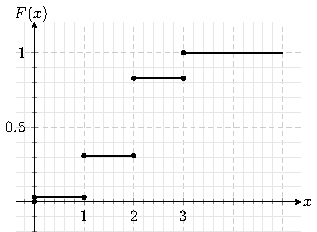
\includegraphics[width=0.5\linewidth]{mai_fig045.pdf}
      \caption{Distribuční funkce k příkladu \ref{mai:exam064}. \cite[s.~233]{Musilova2009MA1}}
      \label{mai:fig045}
    \end{figure}
    Zadáním distribuční funkce je naopak jednoznačně určeno rozdělení veličiny \(X\). Pro jednotlivé
    pravděpodobnosti totiž platí
    \begin{equation*}
      p_j = F(x_j) - F(x_{j-1})\qquad\text{pro}\qquad 2\leq j \leq k, \qquad p_1 = F(x_1).
    \end{equation*}
    
    Hledejme nyní hodnotu \(\overline{x}_P\) definovanou tak, že pravděpodobnost, že při náhodném 
    opakování pokusu nabude veličina \(X\) kterékoli z přípustných hodnot \(x_j \leq 
    \overline{x}_p\), je rovna \(P\). Znamená to, že pro \(x = \overline{x}_P\) má distribuční 
    funkce nabýt předepsané hodnoty \(P\). Abychom \(\overline{x}_P\), takzvaný 
    \(P\)\textbf{-kvantil}, určili, řešíme rovnici
    \begin{equation}\label{mai:eq064}
      \sum_{j=1}^{s}p_j = P
    \end{equation}
    vzhledem k neznámému počtu sčítanců \(s\). V případě veličiny s diskrétním rozdělením se ovšem
    může stát, že pro nevhodně zvolenou hodnotu \(P\) nebude mít rovnice řešení. To proto, že 
    veličina \(X\) může nabývat jen hodnot, které lze očíslovat přirozenými čísly, takže při každé 
    změně horní meze sumy \(s\) o jedničku se suma mění skokem. Vidíme to jak v předcházející 
    tabulce, tak v grafu na obrázku \ref{mai:fig045}. Pro \(P = \num{0.5}\) se \(P\)-kvantil 
    \(\overline{x}_p\), pokud je vůbec definován, nazývá \textbf{medián}. Značí se pouze 
    \(\overline{x}\).

    %--Ještě střelba------------------------------------------------
    % !TeX spellcheck = cs_CZ
\begin{mdframed}[style=mdexam]
  \begin{example}\label{mai:exam067}
    \textbf{Ještě střelba}\newline
    Problém s definici \(P\)-kvantilu u veličiny s diskrétním rozdělením snadno vidíme na příkladu
    střelby (příklad \ref{mai:exam064}). Pro \(s\) postupně 1, 2, 3, 4 nabývá součet na levé straně
    rovnice (\ref{mai:eq064}) hodnot
    
    \begin{equation*}
      p_1 = \num{0.003},\; p_1 + p_2 = \num{0.31},\; p_1 + p_2 + p_3 = \num{0.83}, 
    \end{equation*}
    \begin{equation*}
      p_1 + p_2 + p_3 + p_4 = 1.
    \end{equation*}
    Pojem \(P\)-kvantil je tedy definován jen pro \(P = 0\), \(P = \num{0.03}\), \(P = \num{0.31}\),
    \(P = \num{0.83}\) a \(P = 1\). (Pro \(P = 0\) a \(P = 1\) nemá žádný praktický význam.)
    Nenabývá-li \(P\) žádné z přípustných hodnot, tj. některé hodnoty z množiny \(\{\num{0.03},
    \num{0.31}, \num{0.83}, 1\}\), nemá rovnice pro s řešení a \(P\)-kvantil není vůbec definován.
    Je-li hodnotou \(P\) některý prvek této množiny, dostaneme z rovnice (\ref{mai:eq064}) sice
    jediné řešení \(s\), avšak která hodnota bude \(P\)-kvantilem? Z grafu je vidět, že pro každou
    přípustnou hodnotu \(P\) vyhovuje podmínce celý interval proměnné \(x\). Konkrétní výsledky
    shrnuje následující tabulka:
    
    {\centering
      \begin{tabular}{c|@{\hspace{3pt}}c@{\hspace{3pt}}c@{\hspace{3pt}}c@{\hspace{3pt}}c@{\hspace{3pt}}c}
        \(P\) & \num{0} & \num{0.03} & \num{0.31} & \num{0.83} & \num{1} \\ \hline
        \(F(x) = P\) & \((-\infty,\num{0})\) & \(\left[0, 1\right)\) &
        \(\left[1, 2\right)\) & \(\left[2, 3\right)\) & \(\left[3, \infty\right)\)
      \end{tabular}
    \par}
    
    Význam pojmu \(P\)-kvantil je tedy pro náhodnou veličinu s diskrétním rozdělením poněkud sporný.
    Uplatní se však velmi dobře u veličin s rozdělením spojitým, jak uvidíme později. Než však
    opustíme příklad se střelbou definitivně, spočtěme si ještě střední hodnotu a rozptyl veličiny
    \(X\), kterou jsme definovali jako počet dosažených bodů při jednom výstřelu:
    \begin{align*}
      \langle x \rangle 
          &= \sum_{j=1}^{4}x_jp_j                                                                \\
          &= 0\cdot\num{0.03} + 1\cdot\num{0.28}+ 2\cdot\num{0.52} + 3\cdot\num{0.17} = \num{1.83}, 
    \end{align*}
    \begin{align*}
      D(X)  &= \sum_{j=1}^{4}\left(x_j - \langle x \rangle \right)^2p_j                          \\
            &= (0-\num{1.83})^2\cdot\num{0.03}+(1-\num{1.83})^2\cdot\num{0.28}                   \\
            &+ (2-\num{1.83})^2\cdot\num{0.52}+(3-\num{1.83})^2\cdot\num{0.17}                   \\
                &\simeq\num{0.541},                                                              \\
      \sigma(x) &\simeq\num{0.736}.
    \end{align*}

    V příkladu \ref{mai:exam064} jsme odhadovali, kolika bodů dosáhne střelec při pěti výstřelech.
    Tato hodnota nám vyšla \(\num{5}\cdot\num{1.83} = \num{9.15} = 9\). Nyní vidíme je jí souvislost
    se střední hodnotou náhodné veličiny \(X\). Pokud totiž definujeme veličinu \(Y\) jako počet
    bodů dosažených při pěti výstřelech, je \(Y = 5X\) a \(\langle y \rangle = 5\langle x \rangle\).
    Uvažujme nyní o významu směrodatné odchylky. Zřejmě \(\sigma(y) = 5\sigma(x) = \num{3.68}\).
    Směrodatná odchylka \(\sigma(y)\) určuje interval \((\langle y \rangle - \sigma(y), \langle y
    \rangle + \sigma(y)) = (\num{5.32}, \num{12.68})\). Možnosti bodového zisku ležící v tomto
    intervalu jsou \num{6} až \num{12} bodů včetně. Pokud bychom doplnili tabulku z příkladu
    \ref{mai:exam064} ještě o rozklady a jejich pravděpodobnosti pro bodový součet při pěti
    výstřelech \(j = \num{6}\) a \(j = \num{12}\), dostaneme \(p(A_6) = \num{0.0400}\), \(p(A_{12})
    = \num{0.0550}\). Pravděpodobnost, že výsledek střelce leží při pěti výstřelech v intervalu
    \((\langle y \rangle - \sigma(y), \langle y \rangle + \sigma(y)) = (\num{5.32}, \num{12.68})\),
    je tedy
    \begin{align*}
      \sum_{j=6}^{12}p(A_j) &= p(A_6) + \sum_{j=7}^{11}p(A_j) + p(A_{12})                \\
                            &= \num{0.0400} + \num{0.873} + \num{0.0550} \simeq \num{0.97}.
    \end{align*}
    Při výpočtu jsme využili výsledku z příkladu \ref{mai:exam064}, kde jsme počítali
    pravděpodobnost, že střelec dosáhne bodového výsledku v rozmezí \num{7} až \num{11} bodů.
    Směrodatná odchylka \(\sigma(y)\) veličiny \(Y\) určuje tedy v tomto případě interval okolo
    střední hodnoty \(\langle y \rangle\), v němž leží střelcův bodový zisk s velmi vysokou
    pravděpodobností \SI{97}{\percent}. Tento výsledek lze velmi názorně interpretovat také takto:
    Vystřelí-li střelec pětkrát na terč, bude téměř s jistotou jeho bodový zisk ležet v intervalu
    určeném směrodatnou odchylkou, tj. bude ležet mezi šesti a dvanácti body. Není vyloučeno, že
    bodový zisk bude třeba pět bodů, nebo i nula, nebo naopak dokonce maximálních možných patnáct
    bodů. Všechny ty to možnosti dohromady jsou však vysoce nepravděpodobné, připadá na ně
    pravděpodobnost pouhé \SI{3}{\percent}!. Anebo ještě trochu jinak: Kdyby střelec při tréninku
    uskutečnil třeba sto sérií po pěti výstřelech, pak by skoro jistě bylo sedmadevadesát z nich v
    rozmezí bodového zisku \num{6} až \num{12} bodů a tři mimo. Toto konstatování ovšem opět
    nevylučuje možnost, že v rozmezí \num{6} až \num{12} bodů bude ležet jiný počet sérií než
    \num{97}. Může dokonce v principu dojít k tomu, že do této kategorie padnou série všechny nebo
    žádná. Takový výsledek je však opět vysoce nepravděpodobný.
    
    Není vyloučeno, že i po prostudování tohoto příkladu bude někdo stále nespokojen s tím, že je
    naše vyjadřování „málo přesné“. Vzhledem k pravděpodobnostnímu charakteru posuzovaných jevů
    však, bohužel, přesnější být nemůže.
  \end{example}
\end{mdframed}
    %---------------------------------------------------------------
    
    Příklad \ref{mai:exam067} názorně vypovídá o významu směrodatné odchylky. Viděli jsme, že 
    intervalu o šířce \(2\sigma(y)\) s hodnotou \(\langle y \rangle\) uprostřed odpovídá vysoká 
    pravděpodobnost, že v něm bude ležet bodový zisk střelce při každé pětici výstřelů. Čím bude 
    tento interval užší, tím v průměru blíže budou jednotlivé hodnoty bodového zisku ležet v 
    blízkosti střední hodnoty. Mohli bychom říci, že střelec, jehož výsledky vykazují malou 
    směrodatnou odchylku resp. malý rozptyl, míří přesněji. Směrodatná odchylka je tedy v jistém 
    smyslu jedním z parametrů charakterizujících kvalitu střelby - střelba s malou hodnotou  
    \(\sigma(y)\) je přesnější než střelba s velkou hodnotou \(\sigma(y)\). Druhým parametrem 
    kvality střelby, který je pro její hodnocení z hlediska možnosti vyhrávat soutěže jistě 
    podstatně důležitější, je samozřejmě samotná střední hodnota bodového zisku. Čím je větší, tím 
    je střelcovo pořadí při závodech lepší. Pro interpretaci směrodatné odchylky to ovšem není 
    podstatné. Kdybychom porovnávali dva střelce, jejichž střední bodový zisk při
    pěti výstřelech je třeba \num{12} bodů a \num{3} body, avšak směrodatná odchylka je u obou 
    stejná, musíme konstatovat, že oba jsou stejně přesní. Jeden z nich však systematicky dělá 
    nějakou chybu a přesně střílí do nesprávného místa. Význam pojmu přesnost z hlediska hodnocení 
    náhodných veličin je tedy oproti jeho běžnému chápání poněkud posunut.
    
    Všimněme si ještě jedné důležité obecné věci: Tvar vzorce pro výpočet rozptylu resp. směrodatné 
    odchylky je stejný pro všechny typy rozdělení. Konkrétní pravděpodobnost, že hodnota
    veličiny padne do intervalu určeného směrodatnou odchylkou, tj. do intervalu \((\langle y 
    \rangle - \sigma(y), \langle y \rangle + \sigma(y))\), však pochopitelně na konkrétním 
    rozdělení závisí.

    %--Poissonovo rozdělení-----------------------------------------
    % !TeX spellcheck = cs_CZ
\wikitextrule
\begin{example}\label{mai:exam068}
  \textbf{Poissonovo rozdělení}\newline\small
  Limitním případem Bernoulliova (binomického) rozdělení pro velké hodnoty \(n\), tj. \(n 
  \rightarrow \infty\), a pro \(j \ll n\) je \textbf{rozdělení Poissonovo}. Odvodíme je. Pro velká 
  \(n\) a \(j \ll n\) platí přibližný vzorec
  \begin{equation*}
    n! \simeq n^j(n-j)!,
  \end{equation*}
  a tedy
  \begin{equation*}
    P_j \simeq \lim\limits_{n\rightarrow\infty}\dfrac{n^j}{j!}p^j(1-p)^{n - j}
        \simeq \lim\limits_{n\rightarrow\infty}\dfrac{(np)^j}{j!}\left(1-\dfrac{np}{n}\right)^{n}.
  \end{equation*}
  Při vzpomínce na kapitolu o počítání i limitami a na \textbf{l’Hospitalovo pravidlo} snadno 
  provedeme následující výpočet. O testujte své předchozí znalosti a jednotlivé kroky výpočtu 
  proveďte:
  \begin{equation*}
    \lim\limits_{n\rightarrow\infty}\left(1 - \dfrac{A}{n}\right)^n = 
    \lim\limits_{x\rightarrow0}\left(1 - Ax\right)^\dfrac{1}{x} =
    \exp\left(\lim\limits_{x\rightarrow0}\dfrac{\ln(1 - Ax)}{x}\right) = e^{-A}.
  \end{equation*}
  V našem případě je \(A = np = \langle x \rangle\) (střední hodnota veličiny \(X\) při 
  Bernoulliově rozdělení), takže
  \begin{equation}\label{mai:eq065}
    p_j = \langle x \rangle^j\dfrac{e^{-\langle x \rangle}}{j!}.
  \end{equation}
  Možnost použití Bernoulliova rozdělení si již představit dokážeme. Přinejmenším jsou hody mincemi 
  a kostkami pěkné hříčky. K čemu však je dobré rozdělení Poissonovo? Ja k může vypadat praktická 
  situace, kdy provádíme obrovské množství opakování pokusu a zajímá nás pravděpodobnost pouze 
  malého počtu zdarů? Typickým příkladem takové situace je registrace částic vznikajících při 
  radioaktivním rozpadu. Taková měření jsou potřebná nejen ve fyzikálním výzkumu, ale i v 
  aplikovaných oborech, například v lékařství. Počet \(n\) radioaktivních rozpadů za jednotku času, 
  například za sekundu, je u běžných zdrojů obrovský, zatímco počet těch z nich, které jsou 
  zachycovány detektorem, může být při určitých experimentech malý. Částice se registrují
  pomocí Geigerova-Mullerova počítače, kterým je ionizační komora pracující ve vhodném režimu. 
  Pokud je počet částic \(j\) dopadajících za jednu sekundu do detektoru velmi malý, vyvolá každá z 
  nich měřitelný a dokonce slyšitelný pulz (v obvodu to „praská“). Po registraci částice potřebuje 
  detektor jistou \textbf{mrtvou dobu}, aby se vrátil do výchozího stavu, v němž je schopen 
  registrovat další částici. Tato doba se pohybuje kolem \SI{e-4}{s}. Aby byly jednotlivé pulzy 
  dobře odlišeny, je však třeba, aby do detektoru dopadlo za jednu sekundu mnohem a mnohem méně 
  částic, než jak by odpovídalo převrácené hodnotě mrtvé doby. Zejména pokud bychom chtěli pulzy 
  počítat sluchem, nemělo by jich být více než zhruba jeden až dva každou sekundu. Uvažujme o 
  radioaktivním rozpadu jader cesia \ce{Cs^137}. Jedná se o takzvaný \textbf{beta-rozpad}, který 
  probíhá následovně:
  \begin{itemize}
    \item \ce{Cs^137} \(\longrightarrow\) \ce{Ba^137} + elektron + neutrino, asi \SI{8}{\percent} 
          všech rozpadů
    \item \ce{Cs^137} \(\longrightarrow\) \ce{Ba^137}* + elektron + neutrino, asi \SI{92}{\percent} 
          všech rozpadů
  \end{itemize}
  Excitované baryum \ce{Ba^137}* (jádro má vyšší energii než atom \ce{Ba^137} v základním stavu 
  asi o \SI{0.66}{\mega\electronvolt}  - odpovídá energii \SI{1.1e-13}{\joule}) se pak dále rozpadá 
  podle vzorce
  \begin{itemize}
    \item \ce{Ba137}* \(\longrightarrow\) \ce{Ba137} + částice gama.
  \end{itemize}

  Ze všech částic, které při reakci vznikají, se v Geigerově-Můllerově detektoru registrují 
  elektrony a částice gama, nelze je však od sebe odlišit. Uvažujme o cesiovém zdroji s běžnou 
  hodnotou aktivity, například \SI{10}{\pico\coulomb} (mikrocurie). Jednotka aktivity 
  radioaktivních preparátů \num{1} curie představuje situaci, kdy se za jednu sekundu rozpadá 
  \num{3.7e10} jader. Počet rozpadů, které v průměru nastanou třeba za deset sekund v našem vzorku, 
  je \(n = \num{3700000}\). V Bernoulliově pokusu to odpovídá počtu jeho opakování \(n\). Ja k jsme 
  již řekli, je to obrovský počet. Nastavíme-li experiment tak, abychom registrovali každou sekundu 
  zhruba jednu částici (uslyšíme jeden „prásk“ ), bude počet zdarů \(j\) v Bernoulliově pokusu 
  velmi malý ve srovnání s \(n\). Jsou tedy splněny podmínky pro použití Poissonova rozdělení. 
  Zvolíme například desetisekundový interval měření a počítáme pulzy. Počet registrovaných pulzů 
  \(j\) v tomto intervalu je roven počtu zdarů. Takové měření provedeme třeba dvěstěkrát.
  Označme počet intervalů, v nichž jsme naměřili právě \(j\) pulzů, jako \(\nu(j)\). Celkem je v 
  \(\nu(1) + \cdots + \nu(j_{max}) = \num{200}\). Získáme tak tabulku nebo graf, z nichž pak lze 
  usuzovat na parametry Poissonova rozdělení:
  \begin{table}[ht!]
    \centering
    \resizebox{0.8\textwidth}{!}{%
    \begin{tabular}{c|crrrrrrrrrrrrrrrrr}
      \(j\)      & 0 & 1 & 2 & 3 & 4 & 5 & 6 & 7 & 8 & 9 & 10 & 11& 12& 13 & 14 & 15 & 16 & 17   \\
      \hline
      \(\nu(j)\) & 0 & 4 & 10 & 19 & 28 & 33 & 34 & 26 & 19 & 10 & 6 & 3 & 2 & 2 & 2 & 0 & 1 & 1 \\
    \end{tabular}}
    % \caption{ }
  \end{table}
  Budeme-li předpokládat, že větší počet pulzů v desetisekundovém intervalu je již velmi málo 
  pravděpodobný, můžeme četnosti \(\nu(j)\) považovat za úměrné pravděpodobnostem \(p_j\) 
  Poissonova rozdělení. Všimněme si formule pro Poissonovo rozdělení podrobněji. Je vidět, že platí
  \begin{equation*}
    \dfrac{\nu(j + 1)}{\nu(j)} = \dfrac{p_{j+1}}{p{j}} = \dfrac{\langle x \rangle}{j + 1},
    \qquad p_0 = e^{-\langle x \rangle}.
  \end{equation*}
  Pro hodnotu \(j\), pro kterou jsou si četnosti \(\nu(j)\) a \(\nu(j + 1)\) „nejblíže“, je 
  \(\langle x \rangle \simeq j + 1\). Z tabulky vidíme, že v případě našeho experimentu je 
  \(\langle x \rangle = 6\). Hodnota \(p_0 = e^{-6} \simeq \num{0.002}\) je tedy tak malá, že se 
  ani nedivíme, že jsme mezi dvěma stovkami měření nezaznamenali ani jeden případ, kdy v 
  desetisekundovém intervalu nebyla zaregistrována žádná částice.
  
  Můžeme ještě určit podíly sousedních hodnot \(\nu(j + 1)\) a \(\nu(j)\) a zjistit, zda výsledky 
  našeho experimentu odpovídají vlastnostem Poissonova rozdělení:
  \begin{table}[ht!]
    \centering
    \resizebox{0.7\textwidth}{!}{%
    \begin{tabular}{c|crrrrrrrr}
      \(j\)               & 0 & 1 & 2  & 3  & 4  & 5  & 6  & 7 & 8    \\ \hline
      \(\nu(j+1)/\nu(j)\) & - & \num{2.50} & \num{1.90} & \num{1.47} & \num{1.18} 
                          & \num{1.03} & \num{0.76} & \num{0.73} & \num{0.53}   \\
      \(\langle x \rangle / j + 1\) & \num{6.00} & \num{3.00} & \num{2.00} & \num{1.50} & \num{1.20}
                          & \num{1.00} & \num{0.86} & \num{0.75} & \num{0.67}
    \end{tabular}}
    % \caption{ }
  \end{table}
  \begin{table}[ht!]
    \centering
    \resizebox{0.7\textwidth}{!}{%
    \begin{tabular}{c|crrrrrrrr}
      \(j\)               & 9 & 10 & 11  & 12  & 13  & 14  & 15  & 16 & 17    \\ \hline
      \(\nu(j+1)/\nu(j)\) & \num{0.60} & \num{0.50} & \num{0.67} & - & - & - & - & - & -   \\
      \(\langle x \rangle / j + 1\) & \num{0.60} & \num{0.55} & \num{0.50} & \num{0.46}
                          & \num{0.43} & \num{0.40} & \num{0.38} & \num{0.35} & \num{0.33}
    \end{tabular}}
    % \caption{ }
  \end{table}
  Vidíme, že hodnoty podílů sousedních četností celkem dobře odpovídají vlastnostem Poissonova 
  rozdělení pro \(0 \leq j \leq 12\). Pro \(j > 12\) jsou již četnosti \(\nu(j)\) tak malé, že 
  vytvářet jejich podíly nemá smysl. Tato skutečnost je v tabulce vyznačena pomlčkou.
  
  Poissonovým rozdělením se řídí také například četnost červených krvinek, které se v daném časovém 
  intervalu objeví ve vymezené části zorného pole mikroskopu, četnost zmetků v dodávce zboží, 
  četnost překlepů písařky, apod.  
\normalsize
\end{example}
    %---------------------------------------------------------------
    
    \subsection{Kolik rychlostí má molekula plynu - spojité rozdělení}
      Již nadpis napovídá, že veličina se spojitým rozdělením může zřejmě nabývat „spojitě 
      rozložených“ hodnot, tj. přípustným i hodnotami budou například právě všechna čísla \(x\) z 
      jistého intervalu, \(x\in[a, b]\). Jaká však bude pravděpodobnost \(p(x)\), že veličina \(X\) 
      nabývá právě hodnoty \(x\in[a, b]\)? Jestliže víme, že „součet“ všech \(p(x)\) musí být roven 
      jedné, vzniká problém.
      
      Hodnot \(x\) je totiž nekonečně (dokonce nespočetně) mnoho! Je jich tolik, jako je čísel na 
      celé reálné ose. A kdyby byla pravděpodobnost \(p(x)\) jakkoli malinkatá, nikdy nebude součet 
      všech \(p(x)\) konečný. Pravděpodobnost nabývání hodnoty \(x\) tedy musí být nulová. Vzniklou 
      překážku odstraníme snadno. Rozdělení náhodné veličiny \(X\) bude nutno charakterizovat 
      nikoli pravděpodobností, ale \textbf{hustotou pravděpodobnosti}. Je to obdobná situace jako 
      třeba při popisu rozložení hmotnosti nějakého tělesa, předpokládáme-li, že je ta to hmotnost 
      rozložena v objemu tělesa spojitě. Také nemá příliš smysl se ptát, jaká je hmotnost jednoho 
      bodu tohoto tělesa. I zde by byla odpověď, že nulová. Spíše si vždy klademe otázku, jaká je 
      hmotnost \(\Delta m(\vec{r})\) jistého malého objemu \(\Delta V\), například malého kvádříku, 
      umístěného třeba jedním z vrcholů v bodě o poloze \(\vec{r}\). Hustota \(\varrho(\vec{r})\) 
      tělesa v bodě \(\vec{r}\) je pak limitou podílu \(\Delta m(\vec{r})/\Delta V\) pro \(\Delta V 
      \longrightarrow 0\). Obdobně je tomu i s rozdělením spojité náhodné veličiny \(X\). 
      Zvolíme-li pro jistou hodnotu \(x\) interval \([a, x + \Delta x]\), má smysl otázka, jaké je 
      pravděpodobnost \(\Delta p(x)\), že veličina nabývá hodnoty (kterékoli) právě z tohoto 
      intervalu.

      \adjustbox{minipage=[c]{\textwidth}}{%
        Limitu
        \begin{equation}\label{mai:eq066}
          w(x) = \lim\limits_{\Delta\longrightarrow0}\dfrac{\Delta p(x)}{\Delta x}
        \end{equation}
        nazýváme \textbf{hustotou pravděpodobnosti} veličiny \(X\) v bodě \(x\) (pro \(x = a\), 
        resp. \(x = b\) se jedná o limitu zprava, resp. zleva).
      }
      
      Přímo tato funkce pak představuje ono spojité rozdělení náhodné veličiny \(X\). Určuje totiž
      hustotu pravděpodobnosti \(w\) pro hodnotu \(x\) náhodné veličiny \(X\), obdobně jako \(p_j\) 
      v případě diskrétního rozdělení určuje pravděpodobnost hodnoty \(x_j\). Předpokládejme, že je 
      funkce \(w(x)\) na intervalu \([a, b]\) spojitá.
  
      \adjustbox{minipage=[c]{\textwidth}}{%
        Pro \(x \in [a, b]\) definuje integrál jako funkce horní meze
        \begin{equation}\label{mai:eq067}
          F(x) = \int_a^xw(u)\dd{u}
        \end{equation}
        \textbf{distribuční funkci}.
      }
      Jeho hodnota pro dané \(x\) udává pravděpodobnost, že hodnota veličiny \(X\) padne do 
      intervalu \([a, x]\), opět v plné analogii s případem diskrétního rozdělení. Na \((a, b)\) je 
      tedy hustota pravděpodobnosti \(w(x)\) derivací distribuční funkce. Je zřejmé, že \(F(b) = 
      1\). Integrál z hustoty pravděpodobnosti v mezích \([a, b]\) udává totiž pravděpodobnost, že 
      hodnota veličiny \(X\) padne do intervalu přípustných hodnot, tedy pravděpodobnost jistého 
      jevu. V případě diskrétního rozdělení jsme však distribuční funkci definovali nejen pro 
      přípustné hodnoty náhodné veličiny, ale pro všechna x \in (-\infty, +\infty). Tento postup 
      budeme respektovat i nyní a definujeme
      \begin{equation*}
        F(x) = 0\text{ pro }x \in (-\infty,a)\text{ a }F(x) = 1\text{ pro }x \in (b , +\infty).
      \end{equation*}
      \adjustbox{minipage=[c]{\textwidth}}{%
        \begin{equation}\label{mai:eq068}
          \langle x \rangle = \int_a^bxw(x)\dd{x}, \qquad 
                       D(X) = \int_{a}^{b}(x - \langle x \rangle)^2w(x)\dd{x}.
        \end{equation}
      }
      \textbf{Relativní směrodatná odchylka} je opět podílem \(\sqrt{D(X)}/\langle x \rangle\), 
      nejpravděpodobnější hodnota neboli \textbf{modus} \(x_m\) je taková hodnota veličiny \(X\) , 
      pro kterou je hustota pravděpodobnosti maximální
      
      Daleko lépe než u veličin s diskrétním rozdělením vypadá možnost definovat \(P\)-kvantil 
      \(\tilde{x}_p\) a \textbf{medián} \(\tilde{x}\). Jsou jednoduše řešením rovnic
      \begin{equation*}
        F(\tilde{x}_P) = P, \qquad F(\tilde{x}) = \dfrac{1}{2}
      \end{equation*}
      (Mohli bychom mediánu třeba i říkat „půlkvantil“. To ale není zvykem.) \(P\)-kvantil je 
      definován pro jakoukoli hodnotu \(P\) zadanou v intervalu \((0, 1)\). Skutečně, hustota 
      pravděpodobnosti je nezápornou funkcí na intervalu \([a, b]\) (podle předpokladu i spojitou), 
      takže distribuční funkce je na \([a, b]\) \emph{spojitá} a \emph{rostoucí} a nabývá hodnot 
      \(0 = F(a) \leq F(x) \leq F(b) = 1\). Podle jedné z vět o spojitých funkcích (odstavec 
      2.1.7*) nabývá funkce spojitá na uzavřeném intervalu všech hodnot mezi svým minimem a 
      maximem. V intervalu \([a, b]\) tedy existuje alespoň jedna hodnota \(\tilde{x}_P\) , pro 
      kterou je \(F(\tilde{x}_P) = P\). Ze skutečnosti, že je \(F(x)\) navíc rostoucí, vyplývá, že 
      i \(\tilde{x}_P\) existuje jednoznačně.
  
      Tyto závěry zůstanou v platnosti, i kdyby veličina \(X\) nabývala svých hodnot v intervalu
      typu \(\left[0, \infty\right), \left(—\infty, b\right]\) nebo \((—\infty, \infty)\). Vzhledem 
      k požadavku
      \begin{equation*}
        \int_{a}^{b}w(x)\dd{x} = 1,
      \end{equation*}
      kde kterákoli z mezí \(a\), resp. \(b\) může být i nevlastní, je zřejmé, že funkce \(w(x)\) 
      musí být na svém definičním oboru \(D_f\) omezená. Navíc je na něm spojitá. Vybereme-li tedy 
      jakýkoli uzavřený podinterval oboru \(D_f\), můžeme předchozí argumentaci týkající se 
      \(P\)-kvantilu bez problémů použít.

      %--Normální rozdělení-------------------------------------------
      % !TeX spellcheck = cs_CZ
\begin{mdframed}[style=mdexam]
\begin{example}\label{mai:exam069} \textbf{Normální rozdělení}\\
  Veličinou s normálním rozdělením rozumíme takovou náhodnou veličinu \(X\), jejíž hustota 
  pravděpodobnosti má tvar
  \begin{mdframed}[style=highlight]
    \begin{equation}\label{mai:eq069}
      w(x) = \dfrac{1}{\sigma\sqrt{2\pi}}\exp\left[-\dfrac{(x-\mu)^2}{2\sigma^2}\right],
             \qquad x\in(-\infty, \infty).
    \end{equation}
  \end{mdframed}
  Grafem této funkce je \textbf{Gaussova křivka}. Distribuční funkce má tvar
  \begin{mdframed}[style=highlight]
    \begin{equation}\label{mai:eq70}
      F(x) = \int_{-\infty}^{x}\dfrac{1}{\sigma\sqrt{2\pi}}
               \exp\left[-\dfrac{(t-\mu)^2}{2\sigma^2}\right]\dd{t}.
    \end{equation}
  \end{mdframed}
  udává pravděpodobnost, že hodnota náhodné proměnné je menší než zadaná hodnota (nerovnost může 
  být i neostrá). Přitom \(F(\infty) = 1\) (pravděpodobnost jistého jevu). Skutečně, platí
  \begin{equation*}
    \begin{multlined}
      \int_{-\infty}^{\infty}\dfrac{1}{\sigma\sqrt{2\pi}}
      \exp\left[-\dfrac{(t-\mu)^2}{2\sigma^2}\right]\dd{t}   \\
      \shoveleft[1cm]= \dfrac{\sigma\sqrt{2}}{\sigma\sqrt{2\pi}}
              \int_{-\infty}^{\infty}\exp\left(-u^2\right)\dd{u} =1.
    \end{multlined}
  \end{equation*}
  Takzvaný Laplaceův integrál \(\int_{-\infty}^{\infty}\exp(-u^2)\dd{u} = \sqrt{\pi}\) 
  sice můžeme najít v tabulkách a v dalším dílu jej i odvodíme, v tu to chvíli se však budeme řídit 
  výrokem lorda Kelvina: „Matematik je ten, komu je toto zřejmé jako je zřejmé vám, že dvakrát dvě 
  jsou čtyři.“ Příklady normálního rozdělení pro různé hodnoty \(\sigma,\,\mu\) a odpovídající 
  distribuční funkce vidíme na obrázku \ref{mai:fig046a} a \ref{mai:fig046b}.

  {\centering
    \captionsetup{type=figure}
     \subcaptionbox{\label{mai:fig046a}}{\luafigure[1]{mai_fig046a.pdf}}              \\
     \subcaptionbox{\label{mai:fig046b}}{\luafigure[1]{mai_fig046b.pdf}}
     \captionof{figure}{Hustota pravděpodobnosti normálních rozdělení a jejich distribuční funkce 
              s různými charakteristikami \(\sigma\) a \(\mu\). Červenou čárou je vyznačeno 
              normované normální rozdělení. \cite[s.~240]{Musilova2009MA1}
    \label{mai:fig046}}
  \par}
  \vspace*{10px} Určíme střední hodnotu a rozptyl veličin s tímto rozdělením:
  \begin{align*}
    \langle x \rangle 
      &= \int_{-\infty}^{x}\dfrac{1}{\sigma\sqrt{2\pi}}x\cdot
         \exp\left[-\dfrac{(x-\mu)^2}{2\sigma^2}\right]\dd{x}                                     \\
      &= \dfrac{\sigma\sqrt{2}}{\sigma\sqrt{2\pi}}
         \int_{-\infty}^{\infty}\left(\mu+t\sigma\sqrt{2}\right)\cdot\exp\left(-t^2\right)\dd{t}  \\
      &= \dfrac{\mu}{\sqrt{\pi}}\int_{-\infty}^{\infty}\exp\left(-t^2\right)\dd{t}                \\
      &+ \dfrac{1}{\sqrt{\pi}}\int_{-\infty}^{\infty}t\sigma\sqrt{2}\cdot\exp\left(-t^2\right)\dd{t}
       =\mu.
  \end{align*}
  Druhý z integrálů je totiž roven nule, neboť integrand je lichá funkce.
  \begin{align*}
    D(X)  &= \dfrac{1}{\sigma\sqrt{2\pi}}\int_{-\infty}^{\infty}\left(x - \mu\right)^2 
             \exp\left[-\dfrac{(x-\mu)^2}{2\sigma^2}\right]\dd{x}                                \\
          &= \dfrac{2\sqrt{2}\sigma^3}{\sigma\sqrt{2\pi}}
             \int_{-\infty}^{\infty}t^2\exp\left(-t^2\right)\dd{t}
           = \sigma^2.
  \end{align*}
  Integrál \(\int_{-\infty}^{\infty}t^2\exp\left(-t^2\right)\dd{t} = \frac{\sqrt{\pi}}{2}\) lze buď 
  opět najít v tabulkách, nebo jej metodou per partes převést na výpočet Laplaceova integrálu:
  \begin{align*}
    I &= \int_{-\infty}^{\infty}t\cdot t\exp\left(-t^2\right)\dd{t}         \\
      &= \left[-\dfrac{t}{2}\exp\left(-t^2\right)\right]_{-\infty}^{\infty}
       + \dfrac{1}{2}\int_{-\infty}^{\infty}\exp\left(-t^2\right)\dd{t}.
  \end{align*}
  
  Distribuční funkce normálního rozdělení, zvaná \(errorfunkce\), je běžnou součástí různých 
  počítačových programů, takže poměrně snadno zjistíme pravděpodobnostní obsah intervalu určeného 
  směrodatnou odchylkou \(\sigma(x) = \sqrt{d(X)} = \sigma\). Pravděpodobnost, že hodnota náhodné 
  veličiny \(X\) s normálním rozdělením leží v intervalu \((\mu - \sigma, \mu + \sigma)\), je 
  zhruba \SI{68.3}{\percent}. V souvislosti s normálním rozdělením se často užívají další 
  dva druhy odchylek. \textbf{Pravděpodobná chyba} \(\theta\) určuje interval \((\mu - \theta, \mu 
  + \theta)\), v  němž leží hodnota veličiny \(X\) s pravděpodobností \SI{50}{\percent}. 
  \textbf{Krajní chyba} \(\kappa\) určuje interval \((\mu - \kappa, \mu + \kappa)\), v němž leží 
  hodnota veličiny \(X\) s pravděpodobností \SI{99.7}{\percent}. Z tabelovaných hodnot 
  \(errorfunkce\) zjistíme, že platí
  \begin{equation}\label{mai:eq71}
   \theta \simeq \dfrac{2}{3}\sigma, \qquad \kappa = 3\sigma
  \end{equation}
  Poznamenejme, že normálním rozdělením \(w(x)\) (\ref{mai:eq069}) lze přibližně nahradit 
  Bernoulliovo rozdělení
  \begin{align*}
    w_{Ber}(x)        &= \binom{n}{x}p^x(1 - p)^{n-x},  \\
    \langle x \rangle &= np, \;  D(x) = np(1-p)
  \end{align*}
  pro velké hodnoty \(n\) a také Poissonovo rozdělení
  \begin{equation*}
    w_{Pois}(x) = e^{-\langle x \rangle}\dfrac{\langle x \rangle^x}{x!}, \qquad 
    D(x) = \langle x \rangle
  \end{equation*}
  s velkou střední hodnotou \(\langle x \rangle\)
\end{example}
\end{mdframed}
      %---------------------------------------------------------------
  
      %--Kolik rychlostí má molekula plynu----------------------------
      % !TeX spellcheck = cs_CZ
\wikitextrule
\begin{example}\label{mai:exam070}
  \textbf{Kolik rychlostí má molekula plynu}\newline\small
  Tato otázka se zdá na první pohled zcela nesmyslná. Každý student fyziky ví, že molekuly plynu 
  lze popisovat jako klasické částice, jejichž mechanický stav je jednoznačně určen polohovým 
  vektorem a vektorem rychlosti. Molekula má tedy vždy určitou hodnotu rychlosti. Představte si ale 
  takový plyn ve skutečnosti. Jeden mol jeho látkového množství (např. pro kyslík to představuje 
  hmotnost \num{32} gramů) obsahuje asi \num{6.623e23} molekul! Kdybychom chtěli plyn popisovat 
  jako soustavu klasických částic v mechanice, museli bychom v daném okamžiku znát polohu a 
  rychlost každé molekuly z tohoto obrovského počtu. A to je principiálně nemožné, protože do 
  chování takové soustavy zasahuje velmi podstatným způsobem „náhoda“. Nemůžeme určit, ve kterém
  bodě prostoru právě daná molekula je a jak rychle se pohybuje. Dokážeme pouze určit, s jakou 
  pravděpodobností se nachází v elementárním objemu \(\Delta V = \Delta x \Delta y \Delta z\) v 
  okolí daného bodu o polohovém vektoru \(\vec{r}\) a s jakou pravděpodobností \(\Delta P\) leží 
  koncový bod vektoru její rychlosti v elementárním objemu \(\Delta\Omega = \Delta v_x \Delta v_y 
  \Delta v_z\) „rychlostního“ prostoru v okolí zadané rychlosti \(\vec{v}\). Uvažujme o 
  nejjednodušším modelu plynového tělesa, takzvaném ideálním plynu, jehož molekuly jsou stejné a 
  navzájem neinteragují s výjimkou kratičkých náhodných srážek. Molekuly takového plynu jsou z 
  hlediska pravděpodobnostního popisu navzájem ekvivalentní. Pravděpodobnost \(\Delta P\) bude pro 
  všechny stejná a pro velmi malé elementární objemy bude dána vztahem
  \begin{equation*}
    \Delta P(\vec{r},\vec{v}) = \varrho(\vec{r},\vec{v})\Delta V \Delta\Omega,
  \end{equation*}
  kde \(\varrho(\vec{r},\vec{v}) = \varrho(x, y, z, v_x, v_y, v_z)\) je odpovídající hustota 
  pravděpodobnosti. Jak ale hustota konkrétně závisí na polohách a rychlostech molekul? Tento 
  fyzikální zákon, zvaný \textbf{Gibbsovo rozdělení}, se řídí exponenciální funkcí
  \begin{equation*}
    \varrho(\vec{r},\vec{v}) = K\exp\left(-\dfrac{E(\vec{r},\vec{v})}{kT}\right)
  \end{equation*}
  kde \(E\) je \textbf{mechanická energie molekuly} (kinetická plus potenciální v případném silovém 
  poli), \(T\) je \textbf{absolutní teplota plynu} udávaná v kelvinech a \(k = 
  \SI{1.38e-23}{\joule\per\kelvin}\) je \textbf{Boltzmannova konstanta}.
  
  Zajímá-li vás, proč si příroda v tomto případě vybrala zrovna exponenciální funkci, sledujte 
  následující orientační úvahu: Rozdělme si v myšlenkách plynové těleso na dvě části, jimž 
  odpovídají energie \(E_1\) a \(E_2\). Celková energie soustavy je \(E = E_1 + E_2\). Označme 
  \(P(E)\) pravděpodobnost, že, se soustava nachází ve stavu s energií \(E\), pravděpodobnosti, že 
  se jednotlivé části nachází nezávisle ve stavech s energiemi \(E_1\) a \(E_2\), pak jako
  \(P(E_1)\) a \(P(E_2)\). Pravděpodobnost, že se první část soustavy nachází ve stavu s energií 
  \(E_1\) a \textbf{současně} druhá část ve stavu s energií \(E_2\), je rovna součinu 
  pravděpodobností těchto nezávislých jevů. Proto \(P(E_1 + E_2) = P(E_1) \cdot P(E_2)\). Tuto 
  vlastnost mají ovšem právě exponenciální funkce. Platí tedy \(\varrho \approx\exp(\beta E)\). 
  Konstantu \(\beta\) určí jen experiment, z něhož vychází \(\beta = - (kT)^{-1}\).
  
  Vrátíme se nyní k výchozímu problému, neboť úvodní otázka nabyla smyslu: Molekula může mít 
  libovolnou rychlost s větší či menší pravděpodobností. Nebude-li ideální plyn umístěn v žádném 
  silovém poli, bude mechanická energie molekuly dána pouze energií kinetickou. Elementární 
  pravděpodobnost, že koncový bod rychlosti molekuly leží v elementárním objemu \(\Delta\Omega\) v 
  okolí bodu \(\vec{v}\) „rychlostního“ prostoru, bez ohledu na to, v jaké části „obyčejného“, tj. 
  \textbf{konfiguračního prostoru} se vyskytuje, je
  \begin{equation*}
    \Delta P(\vec{v}) = \varrho(\vec{v})\Delta\Omega 
                      = C\exp\left(-\dfrac{m(v_x^2 + v_y^2 + v_z^2)}{2kT}\right)\Delta\Omega.
  \end{equation*}
  Tato pravděpodobnost, jak je vidět, nezávisí na směru rychlosti, pouze na její velikosti, 
  \(\varrho(\vec{v}) = \varrho(v)\). Konstantu \(C\) určíme snadno. Pravděpodobnost, že molekula má 
  vůbec nějakou rychlost, je rovna jedné (jistý jev). Matematický zápis této skutečnosti vyžaduje 
  znalost takzvaného trojného integrálu (integrujeme podle tří proměnných  - složek vektoru 
  rychlosti). V našem případě se však výpočet redukuje na součin tří integrálů jednoduchých,
  \begin{equation*}
    \int_{\Omega}\varrho(v_x, v_y, v_z)\dd{v_x}\dd{v_y}\dd{v_z} = 1
  \end{equation*}
  \begin{equation*}
    \Rightarrow C \cdot
     \int_{-\infty}^{\infty}\exp\left(\dfrac{mv_x^2}{2kT}\right)\dd{v_x} \cdot
     \int_{-\infty}^{\infty}\exp\left(\dfrac{mv_y^2}{2kT}\right)\dd{v_y} \cdot
     \int_{-\infty}^{\infty}\exp\left(\dfrac{mv_z^2}{2kT}\right)\dd{v_z} =1.
  \end{equation*}
  Po substitucích \(mv_i^2/2kT = u^2,\, i = x, y, z\) vede výpočet na \textbf{Laplaceův integrál}
  \begin{equation*}
    \int_{-\infty}^{\infty}\exp(-u^2)\dd{u} = \sqrt{\pi}.
  \end{equation*}
  Dostáváme
  \begin{equation*}
    C = \left(\dfrac{m}{2\pi kT}\right)^{\frac{3}{2}} \Rightarrow
    \Delta P(\vec{v}) = \left(\dfrac{m}{2\pi kT}\right)^{\frac{3}{2}}
                        \exp\left(- \dfrac{mv^2}{2 kT}\right)\dd{v_x}\dd{v_y}\dd{v_z}
  \end{equation*}
  Hustota pravděpodobnosti je stejná pro všechny koncové body vektoru rychlosti \(\vec{v}\) ležící 
  v rychlostním prostoru na kulové ploše o poloměru rovném velikosti rychlosti \(v\). Jaká bude 
  elementární pravděpodobnost \(\Delta P(v)\), že molekula má velikost rychlosti v intervalu \((v, 
  v + \Delta v)\) bez ohledu na směr pohybu? Tuto pravděpodobnost dostaneme, vezmeme-li za 
  \(\Delta\Omega\) objem tenké kulové slupky o poloměru \(v\) a tloušťce \(\Delta v\), v níž končí 
  všechny vektory rychlosti, jejichž velikost leží v požadovaném intervalu. Tento objem je 
  \(\Delta\Omega = 4\pi v^2\Delta v\) a
  \begin{equation*}
    P(v) = 4\pi\left(\dfrac{m}{2\pi kT}\right)^{\frac{3}{2}}v^2
               \exp\left(- \dfrac{mv^2}{2 kT}\right)\Delta v = f_M(v)\Delta v. 
  \end{equation*}

  {\centering
   \captionsetup{type=figure}
   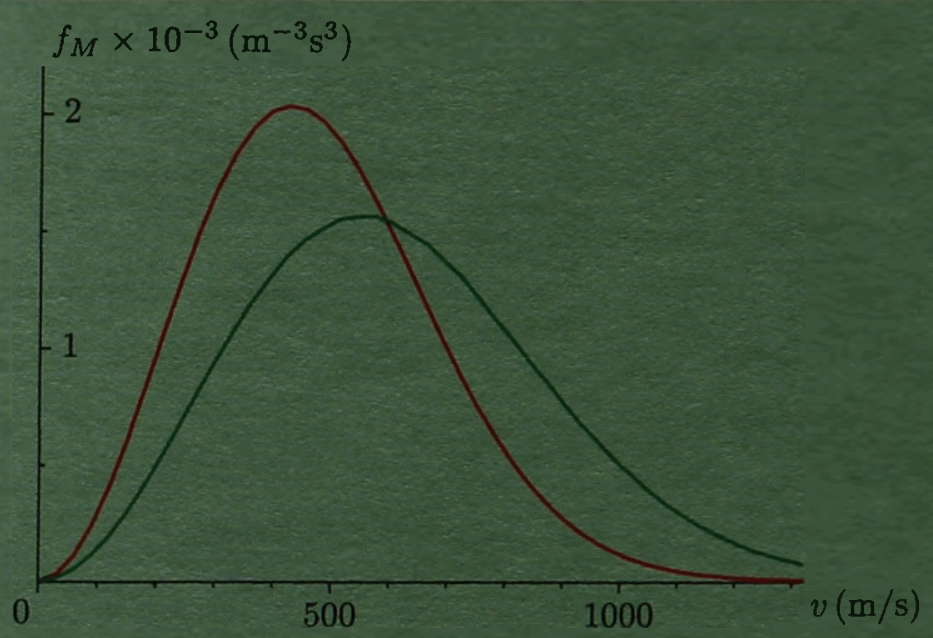
\includegraphics[width=0.4\linewidth]{mai_fig048.png}
   \captionof{figure}{Maxwellovo rozdělení rychlostí molekul dusíku pro teploty \(T_1 = 
                      \SI{300}{\kelvin}\) a \(T_2 = \SI{300}{\kelvin}\).
   \cite[s.~243]{Musilova2009MA1}
   \label{mai:fig048}}
  \par}
  
  Dokážete vyložit, proč jsme zvolili za \(\Delta\Omega\) celý objem slupky? Počítáme totiž 
  pravděpodobnost, že koncový bod vektoru rychlosti molekuly leží, zhruba řečeno, v kterémkoli 
  elementárním kvádříku \(\Delta v_x\Delta v_z\Delta v_z\) obsaženém ve slupce. A ta je součtem 
  pravděpodobností odpovídajících všem kvádříkům vytvářejícím slupku. Jedná se o pravděpodobnosti 
  navzájem neslučitelných jevů (pohybuje-li se molekula v jednom směru, nepohybuje se v jiném). 
  Hustota této pravděpodobnosti se nazývá \textbf{Maxwellovo rozdělení rychlostí}. Na rozdíl od 
  Gaussova rozdělení, popisujícího hustotu pravděpodobnosti pro jednotlivé složky rychlosti, je 
  nesymetrická vlivem faktoru \(v^2\). Obrázek \ref{mai:fig048} ukazuje funkci \(f_M(v)\) pro dvě 
  různé teploty \(T_2 > T_1\). Důležité hodnoty spjaté s tímto rozdělením jsou 
  \textbf{nejpravděpodobnější rychlost} \(v_p\), \textbf{střední rychlost} \(\langle v \rangle\) a 
  \textbf{střední kvadratická rychlost} \(\langle v^2 \rangle\). Platí
  \begin{align*}
    \der{f_M}{v}        &= 0\, \longrightarrow v_P = \sqrt{\dfrac{2kT}{m}},                      \\
    \langle v \rangle   &= \int_{-\infty}^{\infty}vf_M(v)\dd{v} = \sqrt{\dfrac{8kT}{\pi m}},     \\
    \langle v \rangle^2 &= \int_{-\infty}^{\infty}v^2f_M(v)\dd{v} = \dfrac{3kT}{m}.
  \end{align*}
\normalsize
\end{example}
      %---------------------------------------------------------------
  
  \section{Náhoda a zpracování měření}\label{mai:IchapIIIsecIV}
    \subsection{Součet a součin náhodných veličin}
      Nyní vyřešíme ještě jeden důležitý problém. Víme již, že veličinu \(Y = f(X)\) lze popsat 
      stejnými pravděpodobnostmi jako veličinu \(X\). V řadě případů je však náhodná veličina \(Y\) 
      funkcí několika náhodných veličin \(X_1, X_2, \ldots, X_s\). Každá z nich má nějaké 
      rozdělení. Jaké potom bude rozdělení veličiny \(Y\)? Rozebereme jen dvě základní situace, z 
      nichž je ovšem možné „poskládat“ řadu případů složitějších. Půjde o situace, kdy náhodná 
      veličina bude součtem nebo součinem dvou náhodných veličin, pro jednoduchost značení 
      například \(U\) a \(V\), tedy \(Y = U + V\), \(Z = U \cdot V\). Předpokládejme nejprve, že 
      veličiny \(U\) a \(V\) jsou zcela nezávislé, tj. hodnoty veličiny \(U\) nejsou nijak 
      ovlivněny hodnotami veličiny \(V\) a naopak. Dejme tomu, že \(U\) a \(V\) mají rozdělení
      \begin{equation*}
        \left\lbrace (u_1, p_1), \ldots, (u_k, p_k) \right\rbrace, \qquad
        \left\lbrace (v_1, q_1), \ldots, (v_\ell, v_\ell) \right\rbrace
      \end{equation*}
      Veličiny \(Y = U + V\), resp. \(Z = U \cdot V\) tedy mohou nabývat hodnot \(\lbrace u_i + 
      v_\alpha\rbrace\), resp. \(\lbrace u_i v_\alpha\rbrace\) s pravděpodobnostmi \(p_iq_\alpha\). 
      Jevy \uv{Veličina \(U\) nabude hodnoty \(u_i\)} a \uv{veličina \(V\) nabude hodnoty 
      \(v_\alpha\)} jsou totiž nezávislé. Rozdělení veličin \(Y\) a \(Z\) je 
      \begin{equation*}
        \lbrace (u_i +v_\alpha, p_iq_\alpha)\rbrace,\, \text{resp.}\,
        \lbrace(u_iv_\alpha, p_iq_\alpha)\rbrace,\qquad 1\leq i\leq k,\quad 1\leq\alpha\leq\ell,
      \end{equation*}
      Pro jejich střední hodnoty dostáváme
      \begin{align*}
        \langle y \rangle 
          &= \sum_{i=1}^{k}\sum_{\alpha=1}^{\ell}(u_i + v_\alpha)p_iq_\alpha
           = \sum_{i=1}^{k}u_ip_i\left(\sum_{\alpha=1}^{\ell}q_\alpha\right) + 
             \sum_{\alpha=1}^{\ell}v_\alpha q_\alpha\left(\sum_{i=1}^{k}p_i\right)  \\
          &= \sum_{i=1}^{k}u_ip_i + \sum_{\alpha=1}^{\ell}v_\alpha q_\alpha         \\
        \langle z \rangle 
          &= \sum_{i=1}^{k}\sum_{\alpha=1}^{\ell}(u_i \cdot v_\alpha)p_iq_\alpha
           = \left(\sum_{i=1}^{k}u_ip_i\right)
             \left(\sum_{\alpha=1}^{\ell}v_\alpha q_\alpha\right) 
           = \langle u \rangle \langle v \rangle.
      \end{align*}
      Střední hodnota součtu, resp. součinu náhodných veličin je tedy součtem, resp. součinem jejich
      středních hodnot. Pro součet náhodných veličin platí tento výsledek i v případě, když nebudou
      nezávislé. V tak jednoduchý závěr jsme snad ani nedoufali! Hned uvidíme, jak jej lze využít.
      
      %--Jak číst výsledky studentské ankety aneb není průměr jako průměr----------
      % !TeX spellcheck = cs_CZ
\wikitextrule
\begin{example}\label{mai:exam071}
  \textbf{Jak číst výsledky studentské ankety aneb není průměr jako průměr}\newline\small
  Každý semestr na Masarykově univerzitě se uzavírá vyhodnocením velmi užitečné studentské ankety v 
  Informačním systému MU. Studenti hodnotí na jedenáctihodnotové stupnici (nula až deset bodů) 
  několik položek pro každý studijní předmět (obtížnost, zajímavost, srozumitelnost výkladu, 
  přístup učitele, rozmanitost literatury) a mohou doplnit i slovní komentáře. Na ty se učitelé 
  těší nejvíce, neboť díky anonymitě pisatelů se tak o sobě mohou dovědět leccos zajímavého. 
  Všimneme si však statistického zpracování ankety. U každého předmětu je pro danou položku 
  vypočtena průměrná bodová hodnota odpovědí a vyznačena na téže jedenáctihodnotové stupnici. Pro 
  porovnání je na stupnici vyznačen i takzvaný „fakultní průměr“. Každý přednášející může vidět svá 
  hodnocení a hodnocení svých kolegů, kteří mu vedou cvičení. Děkan má přístupové právo k celé
  statistice, a tak může porovnávat. Jednoho deštivého večera přestalo děkana bavit vyplňování 
  rektorátních formulářů a začal si výsledky ankety prohlížet. Zajímala jej zejména položka 
  „srozumitelnost výkladu“. Řekl si, že všem učitelům, kteří v této položce budou hodnoceni 
  nadprůměrně, zvýší osobní ohodnocení. Soubor předmětů je veliký, a tak děkan klikal a klikal. 
  Zjišťoval, že u veliké většiny předmětů leží průměrné hodnocení srozumitelnosti nad fakultním 
  průměrem. Jeho pocity byly smíšené. Na jedné straně se radoval, jakými jsou jeho podřízení 
  dobrými pedagogy, na druhé straně trnul, kolik to bude stát. Snad aby se raději vrátil 
  k protivným formulářům. Najednou v něm zahlodalo podezření i naděje, že není všechno v pořádku. 
  Jak je možné, že většina hodnocení leží nad průměrem? Kladné a záporné odchylky by se přece měly 
  kompenzovat. Zavolal proto na koberec proděkana pro informační technologie, aby se jej zeptal, co 
  je to „fakultní průměr“. Proděkan odpověděl takto: Máme soubor \(K\) předmětů \(\lbrace 
  X_\alpha\rbrace\), \(\alpha = 1, \ldots, K\). V předmětu \(X_\alpha\) vyplnilo anketu 
  \(N_\alpha\)  studentů, jednotlivé hodnoty odpovědí pro danou položku (srozumitelnost výkladu) 
  byly označeny \(\lbrace x_{\alpha,j}\rbrace\), \(j = 1, \ldots, N_\alpha\). Celkem přirozeně 
  předpokládáme, že váha odpovědi každého studenta je stejná, nezávisle na předmětu. Tato váha je
  rovna převrácené hodnotě celkového počtu studentů, kteří vyplnili anketu, tj. \(w = N^{-1}\), \(N 
  = N_1 + \ldots + N_k\). Fakultní průměr je proto dán vzorcem
  \begin{equation*}
    \langle x \rangle 
      = \sum_{\alpha=1}^{K}\sum_{j=1}^{N_\alpha}wx_{\alpha,j} 
      = \dfrac{1}{N}\sum_{\alpha=1}^{K}\left(\sum_{j=1}^{N_\alpha}x_{\alpha,j}\right)
      = \dfrac{1}{N}\sum_{\alpha=1}^{K}A_\alpha,
  \end{equation*}
  kde jsme označili \(A_\alpha = \sum_{j=1}^{N_\alpha}x_{\alpha,j}\). Děkan chvíli přemýšlel a 
  pravil: To vypadá docela logicky. Neměli bychom však počítat fakultní průměr tak, že vezmeme 
  průměrné hodnoty pro každý předmět a vypočteme jejich aritmetický průměr? Pak bychom dostali
  \begin{equation*}
    \langle \overline{x} \rangle
      = \dfrac{1}{K}\sum_{\alpha=1}^{K}\langle x_{\alpha}\rangle
      = \dfrac{1}{K}\sum_{\alpha=1}^{K}
        \left(\dfrac{1}{N_\alpha}\sum_{j=1}^{N_\alpha}x_{\alpha,j}\right)
      = \dfrac{1}{K}\sum_{\alpha=1}^{K}\dfrac{A_\alpha}{N_\alpha}.
  \end{equation*}
  Tento závěr se akademickým funkcionářům na první pohled nijak zvlášť nelíbil. Bylo totiž jasné, 
  že náhodné veličiny \(X_1, \ldots, X_k\) mají odlišná rozdělení. No jo, řekli si oba, musíme 
  počítat. My už ale počítat nemusíme, neboť jsme takový problém před chvílí vyřešili obecně. 
  Zjistili jsme totiž, že střední hodnota součtu náhodných veličin je rovna součtu středních 
  hodnot, bez ohledu na konkrétní rozdělení každé z veličin. Definujeme-li tedy náhodnou veličinu 
  \(Y\) jako aritmetický průměr veličin \(X_\alpha\), tj.
  \begin{align*}
    Y &= \dfrac{1}{K}\left(X_1 + \ldots + X_K\right),  \\
    \shortintertext{dostaneme}
    \langle y \rangle &= \dfrac{1}{K}\left(\langle x_1 \rangle +\ldots+\langle x_K \rangle\right).
  \end{align*}
  Tento výsledek se shoduje s hodnotou \(\langle \overline{x} \rangle\), kterou pro výpočet 
  „fakultního průměru“ navrhl děkan. Vypočteme-li součet odchylek hodnot \(\langle x_\beta 
  \rangle\) od \(\langle y \rangle\), dostaneme skutečně nulu:
  \begin{equation*}
    \sum_{\beta =1}^{K}\left(\langle x_\beta \rangle - \langle y \rangle\right)
      = \sum_{\beta =1}^{K}\left(\dfrac{A_\beta}{N_\beta} 
      - \dfrac{1}{K}\sum_{\alpha=1}^{K}\langle x_\alpha \rangle\right)
      = 0.
  \end{equation*}
  Zkusme se ještě zamyslet nad tím , jak použití „špatného“ fakultního průměru zkreslilo výsledky a 
  proč. Vypočtěme si rozdíl \(\Delta = \langle \overline{x} \rangle - \langle x \rangle\):
  \begin{equation*}
    \Delta = \langle \overline{x} \rangle - \langle x \rangle 
      = \dfrac{1}{K}\sum_{\alpha=1}^{K}\langle x_\alpha \rangle
      - \dfrac{1}{N}\sum_{\alpha=1}^{K}A_\alpha
      = \dfrac{1}{K}\sum_{\alpha=1}^{K}\langle x_\alpha \rangle
      - \dfrac{1}{N}\sum_{\alpha=1}^{K}N_\alpha\langle x_\alpha \rangle
      = \dfrac{1}{K}\sum_{\alpha=1}^{K}\langle x_\alpha\rangle\left(1 - K\dfrac{N_\alpha}{N}\right).
  \end{equation*}
  Platí přitom
  \begin{equation*}
    \sum_{\alpha=1}^{K}\left(1 - K\dfrac{N_\alpha}{N}\right) = 0.
  \end{equation*}
  Pokud by byl počet studentů, kteří vyplnili anketu, ve všech předmětech stejný, tj. \(N_\alpha = 
  \dfrac{N}{K}\) , byla by odchylka \(\Delta\) podle očekávání nulová. Stejná situace by nastala, 
  kdyby byly shodné všechny průměrné hodnoty \(\langle x_\alpha \rangle\). Je-li odchylka 
  \(\Delta\) kladná, je „nesprávný“ fakultní průměr \(\langle x \rangle\) nižší než \(\langle 
  \overline{x} \rangle\). Proto hodnocení jednotlivých předmětů vypadají příznivěji, právě tak, jak 
  to zjistil děkan. Odchylku \(\Delta\) posouvají do kladných hodnot předměty, které hodnotilo málo 
  studentů, a předměty, které měly vysoké hodnocení. Dobře je to vidět na příkladu dvou předmětů, 
  tj. pro \(K = 2\), kde vychází
  \begin{equation*}
    \Delta = \langle \overline{x} \rangle - \langle x \rangle 
           = \dfrac{N_2 - N_1}{2(N_2+N_1)}\left(\langle\overline{x}\rangle-\langle x\rangle\right).
  \end{equation*}
  
  Pro \(N_1\ll N_2\) a \(\langle x_1 \rangle  \gg \langle x_2 \rangle \) bude rozdíl \(\Delta\) 
  skoro polovina hodnoty \(\langle x_1 \rangle\)! U volitelných specializovaných předmětů, které si 
  vybírají jen poměrně malé počty studentů, kteří navíc mají o předmět opravdový zájem a hodnotí 
  jej proto většinou vyšším počtem bodů, je splněno obojí (malý počet hodnotících a vysoké bodové
  hodnocení). Je vidět, že při nesprávně zvoleném výpočtu srovnávací hodnoty (fakultního průměru) 
  mohou právě předměty, jejichž statistický význam je spíše okrajový, ovlivnit celkové hodnocení.
\normalsize
\end{example}
      %----------------------------------------------------------------------------
      
      Pro střední hodnotu součtu a součinu nezávislých náhodných veličin jsme získali velmi
      jednoduché výsledky:
      
      \adjustbox{minipage=[c]{\textwidth}}{%
        \begin{equation}\label{mai:eq070}
          \langle u + v \rangle = \langle u \rangle + \langle v \rangle\qquad
          \langle uv \rangle    = \langle u \rangle \langle v \rangle.
        \end{equation}
      }
      
      Dokážeme také určit rozptyl veličin \(Y = U + V\) a \(Z = U\cdot V\)? Pro rozptyl každé 
      náhodné veličiny platí obecný vztah (\ref{mai:eq061}). Použijeme jej pro naše konkrétní 
      případy:
      \begin{align*}
        D(U + V) &= \langle (u + v)^2 \rangle - \langle u + v \rangle^2 
                  = \langle u^2 + 2uv + v^2 \rangle - \left(\langle u \rangle^2 +
                    \langle 2uv \rangle + \langle v^2 \rangle\right)                        \\
                 &= \left(\langle u^2\rangle - \langle u \rangle^2\right)
                  + \left(\langle v^2\rangle - \langle v \rangle^2\right) = D(U) + D(V).
      \end{align*}
      Pro rozptyl náhodné veličiny \(Z = U \cdot V\) dostaneme
      \begin{align*}
        D(Z)  &= \langle z^2\rangle - \langle z \rangle^2 
               = \langle u^2\rangle\langle v^2\rangle - \langle u \rangle^2 \langle v \rangle^2  \\
              &= \left[D(U) + \langle u^2\rangle\right]\left[D(V) + \langle v^2\rangle\right]
               - \langle u \rangle^2 \langle v \rangle^2                                         \\
              &= D(U)D(V) + \langle u \rangle^2D(V) + \langle v \rangle^2D(U).
      \end{align*}
      Pak
      \adjustbox{minipage=[c]{\textwidth}}{%
        \begin{equation*}
          \dfrac{D(z)}{ \langle z \rangle^2} = \dfrac{D(U)}{ \langle u \rangle^2} \cdot
            \dfrac{D(V)}{ \langle v \rangle^2} + \dfrac{D(U)}{ \langle u \rangle^2} +
            \dfrac{D(v)}{ \langle v \rangle^2}.
        \end{equation*}
      }
      Při výpočtu jsme využili vztahu (\ref{mai:eq061}) a vztahů (\ref{mai:eq070}) pro střední 
      hodnotu součtu a součinu náhodných veličin. Pokud mají veličiny \(U\) a \(V\) shodný rozptyl 
      \(D(U) = D(V) = D\), pak je \(D(U + V) = 2D\). V případě součtu s veličin \(Y = X_1 + \cdots 
      + X_s\) se shodným rozptylem \(D\) resp. směrodatnou odchylkou \(\sigma\) dostáváme
      \begin{equation*}
        D(Y) = sD  \Rightarrow \sigma(y) = \sqrt{s}\sigma.
      \end{equation*}
      Znovu připomeňme, že všechny vztahy týkající se součtu a součinu náhodných veličin, které
      jsme zatím získali, platí za předpokladu, že výchozí veličiny, které sčítáme nebo násobíme, 
      jsou nezávislé.
      
      Aniž bychom se podrobněji zabývali vlastnostmi rozdělení závislých veličin, definujeme pro
      ně charakteristiky, které tuto závislost popisují. Nechť \(U\) a \(V\) jsou dvě libovolně 
      náhodné veličiny, ne nutně nezávislé. Míru jejich závislosti určují veličiny
      \begin{equation}\label{mai:eq071}
        \sigma_{uv} = \langle (u - \langle u \rangle) (v - \langle v \rangle) \rangle, \qquad
        \varrho_ {uv}=\dfrac{\sigma(u)}{\sqrt{D(U)D(V)}} = \dfrac{\sigma(u)}{\sigma{D(u)\sigma(v)}}
      \end{equation}
      zvané \textbf{kovariance} a \textbf{korelační koeficient} veličin \(U\) a \(V\). Platí 
      \(\varrho(uv) \leq 1\). Pro nezávislé veličiny vychází \(\sigma(uv) = 0\) a \(\varrho(uv) = 
      0\).
      
      %-- Rozptyl při Bernoulliově pokusu-----------------------------
      % !TeX spellcheck = cs_CZ
\begin{mdframed}[style=mdexam]
  \begin{example}\label{mai:exam072}
    \textbf{Rozptyl při Bernoulliově pokusu}\newline
    V příkladu \ref{mai:exam066} jsme se zajímali o střední hodnotu veličiny \(X\) definované jako
    počet zdarů při \(n\) opakováních Bernoulliova pokusu. Řekli jsme si, že střední hodnota této
    veličiny je \(np\) s tím, že důkaz lze provést přímo na základě definičního vztahu pro střední
    hodnotu matematickou indukcí. Výpočet rozptylu z definičního vztahu bychom jistě snadno dokázali
    zahájit, horší by však bylo dovést jej do konce. Stačí se podívat na začátek výpočtu
    \begin{align*}
      D(X) &= \sum_{j=0}^n \left(x_j - \langle x \rangle\right)^2p_j             \\
           &= \sum_{j=0}^n \left(j - np\right)^2\binom{n}{j}p^j(1 - p)^j,
    \end{align*}
    a nepochybujeme o tom, že tuto sumu nedokážeme spočítat snadno. Protože již však umíme zacházet
    se součtem náhodných veličin, můžeme využít účinného triku. Veličinu \(X\) si představíme jako
    součet
    \begin{equation*}
      X = U_1 + U_2 + \cdots + U_n,
    \end{equation*}
    kde každá z veličin \(U_j\) může nabývat dvou hodnot. Jedničky v případě, že při \(j\)-tém
    opakování pokusu nastal zdar, a nuly v případě, že nastal nezdar. Součet všech veličin \(U_j\)
    pro \(j = 1\) až \(j = n\) pak skutečně znamená celkový počet zdarů při \(n\) opakováních
    pokusu. Jestliže si uvědomíme, že pravděpodobnost zdaru při kterémkoli z opakování je \(p\) a
    pravděpodobnost nezdaru \((1 - p)\), ihned vidíme, že rozdělení každé z veličin \(U_j\) má tvar
    \(\lbrace(1, p), (0, 1 - p)\rbrace\). Platí tedy
    \begin{equation*}
      \langle u_j\rangle = 1\cdot p + 0 \cdot (1 - p) = p,
    \end{equation*}
    \begin{align*}
      D = D(U_j) &= \left( 1 - \langle u_j\rangle\right)^2p 
                  + \left( 0 - \langle u_j\rangle\right)^2(1 - p)   \\
                 &= p(1 - p)^2 + p^2(1 - p) = p(1 - p).
    \end{align*}
    Každé dvě veličiny \(U_i\), \(U_j\) jsou nezávislé, neboť jednotlivá opakování pokusu jsou
    nezávislá. Střední hodnota jejich součtu je: tedy \(np\) (a to souhlasí s informací v příkladu
    \ref{mai:exam066}) a pro rozptyl jejich součtu platí
    \begin{equation*}
      D(X) = nD = np(1 - p).
    \end{equation*}
    Celkově tedy dostáváme
    \begin{equation*}
      \langle x \rangle = np, \; \sigma(x) = \sqrt{np(1 - p)}.
    \end{equation*}
  \end{example}
\end{mdframed}
      %---------------------------------------------------------------
      
      %-- Rozptyl aritmetického průměru-------------------------------
      % !TeX spellcheck = cs_CZ
\begin{mdframed}[style=mdexam]
  \begin{example}\label{mai:exam073}
    \textbf{Rozptyl aritmetického průměru}\newline
    Již v úvodu odstavce o náhodných veličinách jsme konstatovali, že opakujeme-li v nezměněných
    podmínkách měření jisté fyzikální veličiny (délka závěsu kyvadla, proud procházející vodičem,
    napětí na vodiči, atd.), budeme díky náhodným vlivům dostávat pokaždé poněkud jiný výsledek.
    Říkáme, že měření je zatíženo náhodnými chybami. Výsledek získaný při každém opakování lze
    interpretovat jako hodnotu náhodné veličiny. Dejme tomu, že jsme provedli uměření fyzikální
    veličiny \(X\) a získali hodnoty \(x_1\) až \(x_n\) . V praktické situaci budou tyto hodnoty
    většinou navzájem různé, nemusí tomu tak však nutně být. Fyzikální veličinu chceme ovšem
    reprezentovat jediným údajem, a tím bude její střední hodnota, tj.
    \textbf{aritmetický průměr}
    \begin{equation*}
      \langle x \rangle = \dfrac{x_1 + x_2 + \cdots + x_n}{n}.
    \end{equation*}
    Rozptyl veličiny \(X\) je dán vztahem
    \begin{align*}
      D &= D(X)                                                             \\
        &= \dfrac{\left(x_1 - \langle x \rangle\right)^2 + 
                  \left(x_2 - \langle x \rangle\right)^2 + \cdots +
                  \left(x_n - \langle x \rangle\right)^2}{n}.
    \end{align*}
    Víme, že směrodatná odchylka \(\sigma( x ) = \sqrt{D(X)}\) určuje, nakolik jsou jednotlivé
    výsledky měření v průměru odchýleny od střední hodnoty, charakterizuje tedy přesnost každého
    opakování měření. Podívejme se na celou úlohu z jiné strany: Představme si, že sledujeme \(n\)
    po dvou nezávislých náhodných veličin \(X_1\) až \(X_n\) se shodnou střední hodnotou \(\langle
    x_j \rangle = \langle x \rangle\) a shodnou směrodatnou odchylkou \(\sigma(x_j) = \sqrt{D},\, 1
    \leq j \leq n\). Aritmetický průměr těchto veličin,
    \begin{equation*}
      \langle \Xi \rangle = \dfrac{X_1 + X_2 + \cdots + X_n}{n}.
    \end{equation*}
    je tedy rovněž náhodnou veličinou. Pro jeho střední hodnotu, rozptyl a směrodatnou odchylku
    platí
    \begin{align*}
      \langle \xi \rangle 
                  &= \dfrac{n\langle x \rangle}{n}, \\
      D(\Xi)      &= \dfrac{1}{n^2}\cdot D(X_1 + \cdots + X_n)=\dfrac{nD^2}{n^2}=\dfrac{D}{n}, \\
      \sigma(\xi) &= \dfrac{\sigma(x)}{\sqrt{n}}.
    \end{align*}
  \end{example}
\end{mdframed}
      %---------------------------------------------------------------
      
      Můžeme tedy říci, že aritmetický průměr všech výsledků měření dané fyzikální veličiny je
      \(\sqrt{n}\)-krát přesnější než jednotlivý výsledek měření. Jakkoli se toto konstatování zdá 
      intuitivně zřejmé, je třeba je používat s opatrností.
      
      Především je třeba mít na mysli, co toto konstatování znamená. Jeho charakter je totiž
      opět jen pravděpodobnostní. Jestliže jsou jednotlivá měření prováděna za stejných podmínek,
      jsou rozdělení veličin \(X_1\) až \(X_n\) funkcemi téhož typu. Tyto veličiny mají také 
      stejnou střední hodnotu \(\langle x \rangle\) a směrodatnou odchylku \(\sigma\). Také 
      pravděpodobnost, že při měření padne hodnota veličiny \(X_j\) do intervalu \((\langle x 
      \rangle - \sigma, \langle x \rangle + \sigma)\), je pro všechna \(j\) prakticky stejná. 
      Označme ji \(P_\sigma\).  Se stejnou pravděpodobností nabude aritmetický průměr \(\Xi\) 
      hodnoty v intervalu určeném svou směrodatnou odchylkou. Ta je však \(\sqrt{n}\)-krát menší. V 
      tomto smyslu jsou hodnoty aritmetického průměru \uv{\(\sqrt{n}\)-krát méně rozptýleny} kolem 
      střední hodnoty \(\langle\xi \rangle\) než hodnoty náhodných veličin \(X_j\) kolem svých 
      středních hodnot \(\langle x \rangle\).
      
      Dalším problémem může být splnění výchozích předpokladů, které vedly ke vztahu pro
      směrodatnou odchylku aritmetického průměru. Ukážeme to na následujícím příkladu.
      
      %-- Jak přesně lze změřit čínského císaře?----------------------
      % !TeX spellcheck = cs_CZ
\wikitextrule
\begin{example}\label{mai:exam075}
  \textbf{Ověření Ohmová zákona}\newline\small

\normalsize
\end{example}
      %---------------------------------------------------------------
      
      %-- Záhada přijímací zkoušky aneb k čemu může posloužit distribuční funkce-----
      % !TeX spellcheck = cs_CZ
\begin{mdframed}[style=mdexam]
  \begin{example}\label{mai:exam075}
    \textbf{Záhada přijímací zkoušky aneb k čemu může posloužit distribuční funkce?}\newline
    Mohlo by se zdát, že distribuční funkce je jen teoretický pojem a že v praktických situacích ji
    těžko využijeme. Podstatné je přece pravděpodobnostní rozdělení náhodné veličiny a distribuční
    funkce je z něj jen jaksi odvozena sčítáním pravděpodobností (u diskrétního rozdělení) nebo
    integrací (u rozdělení spojitého). Přesvědčíme se, že existují velmi realistické případy, kdy
    distribuční funkce přináší věrohodnější informaci o náhodné veličině než samotné rozdělení.
    
    Na Masarykově univerzitě musí každý uchazeč o studium, ať již se hlásí na přírodovědeckou,
    právnickou, lékařskou či jinou fakultu, absolvovat Test studijních předpokladů. Jedná se o
    všeobecný test, zaměřený na zjišťování úrovně všech schopností uchazeče, které jsou potřebné pro
    univerzitní studium, například analytického myšlení, verbálních schopností, numerického myšlení,
    geometrické představivosti, atd. Pro nás však v tu to chvíli není podstatný obsah testu, ale
    způsob zpracování jeho výsledků a vyhodnocení pořadí uchazečů. Test skládá kolem třiceti tisíc
    studentů. Není tedy možné technicky zajistit, aby proběhl v jediné variantě v jednom dni. K
    dispozici je proto osm variant testu, každou variantu řeší tři až čtyři tisíce studentů. Test má
    \num{80} otázek, základním údajem pro zpracování jeho výsledků je počet správných odpovědí
    každého studenta. Pokud bychom označili jako \(i\) počet správných odpovědí (\(i \in\lbrace0, 1,
    2, \ldots, 80\rbrace\)) v kterékoli variantě a \(\mathcal{N}_i\) počet studentů, kteří dosáhli
    právě \(i\) správných odpovědí, dostaneme náhodnou veličinu \(X_i\), kterou bychom mohli nazvat
    „počet správných odpovědí“, pro celou univerzitu. Její rozdělení by mělo tvar
    \begin{equation*}
      \lbrace(i,p_i)\rbrace,\quad\text{kde}\qquad p_i = \dfrac{\mathcal{N}_i}{\mathcal{N}}, \quad
      \mathcal{N} = \sum_{i=0}^{80}\mathcal{N}_i
    \end{equation*}
    A zde je malý „kámen úrazu“. A by bylo možné sestavit opravdu „univerzální pořadí“, musely by
    být všechny varianty testu ekvivalentní z hlediska obtížnosti. To znamená, že kdyby kterýkoli
    student vyplnil za stejných podmínek všechny varianty, dosáhl by v každé z nich stejného počtu
    správných odpovědí s pravděpodobností velmi blízkou jedné. Skutečnost je však principiálně
    taková, že u sebelépe promyšleného a sestaveného testu se jednotlivé varianty budou mírně, v
    rámci statistických, a tedy již neodstranitelných, odchylek lišit. Tato odlišnost se nepozná
    předem, ale až po zpracování výsledků všech variant. Použít pro stanovení pořadí uchazečů
    rozdělení náhodné veličiny \(X\) \emph{= počet správných odpovědí je tedy nespravedlivé}.
    Student, který řešil variantu „statisticky obtížnější“, by v pořadí skončil s horším umístěním,
    než student, který je stejně schopný, avšak měl to štěstí, že na něj připadla varianta
    „statisticky méně obtížná“. Skutečně, kdybychom sestavili grafy rozdělení náhodných veličin
    \(X^{(\alpha)}\) \emph{= počet správných odpovědí v \(\alpha\)-té variantě},
    \begin{equation*}
      \lbrace(i,p_i^{(\alpha)})\rbrace,\quad\text{kde}\; 
      p_i^{(\alpha)} = \dfrac{\mathcal{N}_i^{(\alpha)}}{\mathcal{N}^{(\alpha)}}, \quad
      \mathcal{N}^{(\alpha)} = \sum_{i=0}^{80}\mathcal{N}_i^{(\alpha)}
    \end{equation*}
    zjistili bychom, že se mírně liší. (V předchozím zápisu značí \(\mathcal{N}_i^{(\alpha)}\) počet
    studentů, kteří odpověděli správně na \(i\) otázek \(\alpha\)-té varianty
    \(\mathcal{N}^{(\alpha)}\) je počet všech studentů, kteří tuto variantu řešili.) Střední hodnoty
    i mediány náhodných veličin se i při vynikající shodě obtížnosti všech variant mohou lišit v
    rozmezí jedné až dvou správných odpovědí. A s ohledem na skutečnost, že každou variantu řeší
    obrovský počet studentů, až čtyři tisíce, je zřejmé, že tento rozdíl může poněkud „zamíchat
    “pořadím, zejména v blízkosti mediánu, kde se týká třeba i tří stovek studentů v každé variantě.
    Situaci dokládá obrázek \ref{mai:fig049}. Jak tedy zařídit, abychom dostali spravedlivé pořadí?
    Jediný rozumný způsob, jak minimalizovat vliv statistických odchylek obtížnosti jednotlivých
    variant, je nehodnotit studenty podle absolutního počtu správných odpovědí, ale nějak je
    porovnat mezi sebou. Budeme při tom předpokládat, že rozložení schopností studentů je ve všech
    osmi skupinách, které řeší osm daných variant, stejné. Řeknete si - zase nějaké další
    předpoklady. To je jako z bláta do louže. Předpoklad o stejném rozložení schopností studentů v
    tak velkých skupinách, jako jsou ty naše, je však mnohem realističtější než předpoklad o
    dokonalé shodě obtížnosti variant testu. Budeme se jej proto držet. Každému studentovi
    přisoudíme číslo, které informuje o tom, kolik řešitelů dané varianty bylo horších nebo stejně
    dobrých jako on, tj. mělo nižší nebo stejný počet správných odpovědí. Z matematického hlediska
    to znamená přejít v každé variantě od rozdělení k distribuční funkci. Věnujme se nyní tomuto
    přepočtu podrobněji jak pro diskrétní rozdělení náhodné veličiny \(X^{(\alpha)}\), které
    odpovídá skutečné situaci, tak pro zajímavost i pro rozdělení spojité. V dalším budeme vždy
    zpracovávat výsledky jedné varianty, upustíme proto od vyznačování indexu \(\alpha\).

    {\centering
    \captionsetup{type=figure}
    \luafigure[0.8]{mai_fig049.png}
    \captionof{figure}{Rozdělení pro dvě varianty testu,
    \cite[s.~252]{Musilova2009MA1}
    \label{mai:fig049}}
    \par}
    
    \textbf{Diskrétní rozdělení}
      \begin{itemize}
        \item \emph{Zadání:} Skupina \(N\) studentů řeší jednu variantu testu. Test má \(Q\) otázek.
              Za každou správnou odpověď je přidělen jeden výchozí bod. Získáváme rozdělení
              \begin{gather*}
                \left\lbrace\left(i, \dfrac{N_i}{N} \right)\right\rbrace, \;
                i\in\lbrace0, 1, 2, \ldots, Q\rbrace, \;
                \sum_{i=0}^{Q}N_i = N 
              \end{gather*}
              kde \(i\) je počet výchozích bodů a \(N_i\) počet studentů, kteří získali \(i\) bodů.
              Distribuční funkce tohoto rozdělení
              \begin{gather*}
                F(x) = \dfrac{1}{N}\sum_{i=0}^{j}N_i\;\text{ pro }\;
                j\leq x < j+1, \; x\in\left[0,\infty\right)
              \end{gather*}
              Pro uchazeče, který získal \(j\) bodů, mají význam následující hodnoty:
              \begin{itemize}
                \item \(F(x)    x \in \left[j, j+1\right)\): poměrný počet uchazečů, kteří získali
                      počet výchozích bodů nižší nebo shodný s daným uchazečem,
                \item \(NF(x)   x \in \left[j, j+1\right)\): absolutní počet uchazečů, kteří získali
                      počet výchozích bodů nižší nebo shodný s daným uchazečem,
                \item \(100F(x) x \in \left[j, j+1\right)\): absolutní počet uchazečů, kteří získali
                      počet výchozích bodů nižší nebo shodný s daným uchazečem,
              \end{itemize}
        \item Hodnoty distribuční funkce můžeme získat z následující tabulky:
        
              {\centering
                \resizebox{0.8\textwidth}{!}{%
                \begin{tabular}{c|c}
                          interval \(x\)     &  \(NF(x)\)         \\ \hline
                  \(\left[0,1\right)\)       &  \(N_0\)           \\ 
                  \(\left[1,2\right)\)       &  \(N_0 + N_1\)     \\ 
                  \(\cdots\)                 &  \(\cdots\)        \\
                  \(\left[j,j+1\right)\)     &  \(N_0 + N_1 + \cdots + N_j\) \\ 
                  \(\cdots\)                 &  \(\cdots\) \\
                  \(\left[Q-1,Q\right)\)     &  \(N_0 + N_1 + \cdots + N_{Q-1}\) \\ 
                  \(\left[Q,\infty\right)\)  &  \(N_0 + N_1 + \cdots + N_{Q} = N\) 
                \end{tabular}}
              \par}
        \item Přepočet hodnocení uchazečů tak, aby nová stupnice byla opět v rozsahu mezi nulou a
              \(Q\) a aby nové hodnocení bylo opět celočíselné, je následující:
              \begin{equation*}
                y =QF(x), \quad 0\leq F(x) \leq 1, \Rightarrow y \in[0,Q].
              \end{equation*}
              Uchazeči se ziskem \(i\) výchozích bodů náleží hodnota \(y = QF(x)\) právě když i\(
              \in \left[i, i + 1\right)\), tj. \(y_i = Q F(i)\). Tato hodnota není obecně
              celočíselná. Zaokrouhlení se provede ve prospěch uchazeče, tedy vždy nahoru. Výsledný
              převodní vzorec je
              \begin{equation*}
                \begin{multlined}
                  \text{výchozí body } i \longrightarrow\text{ nové body }  \\ 
                  \shoveleft[1cm]Y_i: Y_i = [y_i] + 1 = [QF(i)] + 1,
                \end{multlined}
              \end{equation*} 
              kde \([a]\) značí celočíselnou část čísla \(a\), tedy například \([\num{23.05}] =
              [\num{23.48}] = [23,89] = 23\)
        \item Zaveďme novou náhodnou veličinu \(Z\) s rozdělením \(\left\lbrace(z_\alpha,
              M_\alpha)\right\rbrace\): Označme \(z_1, z_2, \ldots, z_\alpha, ...,\) \(z_S\)
              navzájem různé hodnoty ze souboru \(\lbrace Y_i\rbrace, i = 0, 1, 2, \ldots, Q\)
              řazené vzestupně. Její rozdělení udává kterákoli z následujících tabulek:

              {\centering
                \resizebox{0.9\textwidth}{!}{%
                \begin{tabular}{c|c}
                          hodnota                       &  četnost         \\
                          \hline
                  \(z_1 = Y_0 = Y_1 = \cdots Y_{i_1}\)  & \(M_1 = N_0 + N_1 + \cdots + N_{i_1}\)  \\ 
                  \(Z_2 = Y_{i_1+1} = \cdots Y_{i_2}\)  & \(M_2 = N_{i_1+1} + \cdots + N_{i_2}\)  \\ 
                  \(\cdots\)                            & \(\cdots\)                              \\
                  \(Z_S = Y_{i_{S-1}+1}=\cdots Y_{i_S}\)& \(M_S = N_{i_{S_1}+1}+\cdots+N_{i_S}\)   
                \end{tabular}}
              \par}

              {\centering
                \resizebox{0.9\textwidth}{!}{%
                \begin{tabular}{c|c}
                          hodnota                        &  četnost         \\
                          \hline
                  \(z_1 = Y_0 = Y_1 = \cdots Y_{i_1}\)   &  \(M_1 = NF(i_1)\)              \\
                  
                  \(Z_2 = Y_{i_1+1} = \cdots Y_{i_2}\)   &  \(M_2 = N[F(i_2) - F(i_1)]\)  \\ 
                  \(\cdots\)                             &  \(\cdots\)                     \\
                  \(Z_S = Y_{i_{S-1}+1}=\cdots Y_{i_S}\) & \(M_S = N[F(i_S) - F(i_{S-1})]\)   
                \end{tabular}}
              \par}
              kde \(i_1 < i_2 < \ldots < i_{S-1} < i_S, i_S = Q\) (Vzhledem k zaokrouhlování nahoru
              není žádná bodová hodnota \(Y_i\) nulová.) I když skutečné rozdělení při zpracování
              výsledků testů je diskrétní, ukažme si, jak by vypadal analogický postup u rozdělení
              spojitého, kde je početní zpracování názornější.
      \end{itemize}
    
    \textbf{Spojité rozdělení}
      \begin{itemize}
        \item \emph{Zadání:} Je dáno rozdělení četností \(n(x) \leq 0,\, x \in [0, Q]\).
        \item Normovací podmínka a distribuční funkce jsou
              \begin{equation*}
                \int_{0}^{Q}n(x)\dd{x} = N, \quad 
                F(x) = \dfrac{1}{n}\int_{0}^{x}n(\xi)\dd{\xi},                
              \end{equation*}
              kde \(0 \leq F(x) \leq 1.\)
        \item Označme \(z = QF(x)\), tedy \(z \in [0, Q]\), novou náhodnou veličinu. (Uvědomme si,
              že \(z\) je rostoucí funkcí proměnné \(x\)). Označme její rozdělení \(\nu(z)\). Její
              distribuční funkce je
              \begin{align*}
                \Phi(z) &= \int_{0}^{z}\nu(\zeta)\dd{\zeta} 
                         = \int_{0}^{x(z)}\dfrac{n(\xi)}{N}\dd{\xi}          \\
                        &= F\left(F^{-1}(z/Q)\right) 
                        = \dfrac{z}{Q}, \quad
                \nu(z) = \dfrac{1}{Q}.
              \end{align*}
        \item Rozdělení je konstantní s mediánem i střední hodnotou \(Q/2\). Takové rozdělení se
              nazývá rovnoměrné.
      \end{itemize}
  \end{example}
\end{mdframed}
      %------------------------------------------------------------------------------
      
    \subsection{Který výsledek je ten pravý?}
      První věc, kterou budete dělat ve fyzikálním praktiku, bude zjišťování průměrné hustoty 
      materiálu, z něhož je vyroben kovový váleček. Budete váleček vážit, abyste určili jeho 
      hmotnost,a měřit jeho výšku a průměr, abyste mohli vypočítat jeho objem. Hustotu stanovíte 
      jako podíl hmotnosti a objemu. Jedná se stále o jeden a týž váleček, jehož průměrná hustota 
      má za daných podmínek (stálá teplota, váleček se nedeformuje, apod.) stále stejnou „správnou“ 
      hodnotu, kterou však neznáme. (Nezná ji ani učitel v praktiku, i když se tak tváří.) Změří-li 
      hustotu válečku všichni studenti ve skupině, každý jen jednou, získá se řada různých hodnot. 
      Která z nich je ta správná? Není vyloučeno, a je to dokonce velmi pravděpodobné, že žádná. A 
      mohli bychom pomocí nich správnou hodnotu určit nebo se k ní alespoň přiblížit? Možné by to 
      bylo, pokud bychom zaručili, že všechny výsledky získané jednotlivými studenty jsou „stejně 
      hodnotné“. Znamenalo by to, že bychom museli vyloučit hrubé a systematické chyby, které by 
      vznikly třeba tak, že by někteří studenti vážili na vadných vahách, někteří by měli špatné 
      měřítko, popřípadě by odečítali údaj „zboku“, takže by byl zkreslený, nebo by se dokonce 
      zmýlili při odečítání údaje. Museli bychom také zaručit, že náhodné vlivy, které ovlivňují 
      měření, zatěžují je náhodnými chybami a v principu je nelze odstranit, byly při všech 
      měřeních stejné. U různých studentů si tím však nemůžeme být jisti (vzpomeňte si na měření 
      čínského císaře), proto budeme raději postupovat tak, že jeden pečlivý student provede větší 
      počet měření třeba výšky válečku, která je pro určení hustoty potřebná. Dejme tomu, že bude 
      měřit milimetrovým měřítkem a bude odhadovat s přesností na půl milimetru. Jeho údaje tedy 
      mohou mít tvar \SI{33.0}{\mm}, \SI{34.5}{\mm}, atd. Získá takto za stejných podmínek třeba 
      dvacet nebo i padesát hodnot, ale co teď s nimi? Jak určit hodnotu, která se bude nejvíce 
      blížit správné hodnotě výšky válečku? (Dalo by se jistě diskutovat i o tom, co je to správná 
      hodnota. Pro tuto chvíli však předpokládejme, že taková hodnota skutečně existuje, neboť 
      váleček je opravdu válcem, je vysoustružen pečlivě, přesněji, než jsme schopni jej měřit, při 
      měření se nemění teplota, váleček není dáván do lisu a deformován, ani upravován tak, že by 
      se měnila jeho hmotnost.) Předpokládejme, že správná hodnota výšky válečku je \(x\) a že 
      student naměřil hodnoty \(\lbrace x_1, X_2, \ldots, x_n\rbrace\), mezi nimiž mohou být 
      pochopitelně i některé hodnoty stejné. Odchylky jeho měření od správné hodnoty jsou
      \begin{equation*}
        \lbrace \varepsilon_1, \varepsilon_2, \ldots, \varepsilon_n\rbrace, \qquad
        \varepsilon_i = x_i - x, \qquad i = 1, 2, \ldots, n.
      \end{equation*}
      I kdybychom správnou hodnotu \(x\) znali, nedokázali bychom předpovědět, nakolik se od ní při
      jednotlivém měření odchýlíme. Můžeme, se však zajímat o to, jaká je pravděpodobnost, že
      hodnota, o kterou bude měření od správné hodnoty odkloněno, bude ležet v určitém intervalu.
      Odchylky \(\varepsilon_i\) lze totiž interpretovat jako hodnoty náhodné veličiny. Abychom 
      mohli požadované pravděpodobnosti určit, potřebujeme znát rozdělení této veličiny. Označme ji 
      \(\varepsilon\) a odpovídající hustotu pravděpodobnosti \(\mathcal{w}(\varepsilon)\). Toto 
      rozdělení je za určitých podmínek \textbf{rozdělením normálním}, splňuje tedy vztah 
      (\ref{mai:eq069}). Zkusme se o tom přesvědčit. Zvolme podmínky měření tak, aby byly ve hře 
      jen náhodné chyby způsobené \(m\) nezávislými vlivy. Každý z nich hodnotu měření
      odchýlí od \(x\) o stejně velkou hodnotu \(\alpha\), kladnou nebo zápornou, s 
      pravděpodobností \num{0.5}. Schéma této úvahy je na obrázku \ref{mai:fig050}. Výsledná 
      odchylka naměřené hodnoty \(x_i\) od hodnoty správné s jistotou leží v intervalu \((-m\alpha, 
      m\alpha)\) a může nabývat pouze hodnot celých násobků \(\alpha\). Při uplatnění jednotlivého 
      „chybového“ vlivu vzniká, jak jsme již řekli, kladná nebo záporná odchylka o velikosti 
      \(\alpha\). Vznik odchylky \(+\alpha\) nazveme zdarem, vznik odchylky \(-\alpha\) nezdarem.
      
      \begin{figure}[ht!] %\ref{mai:fig050}
        \centering
        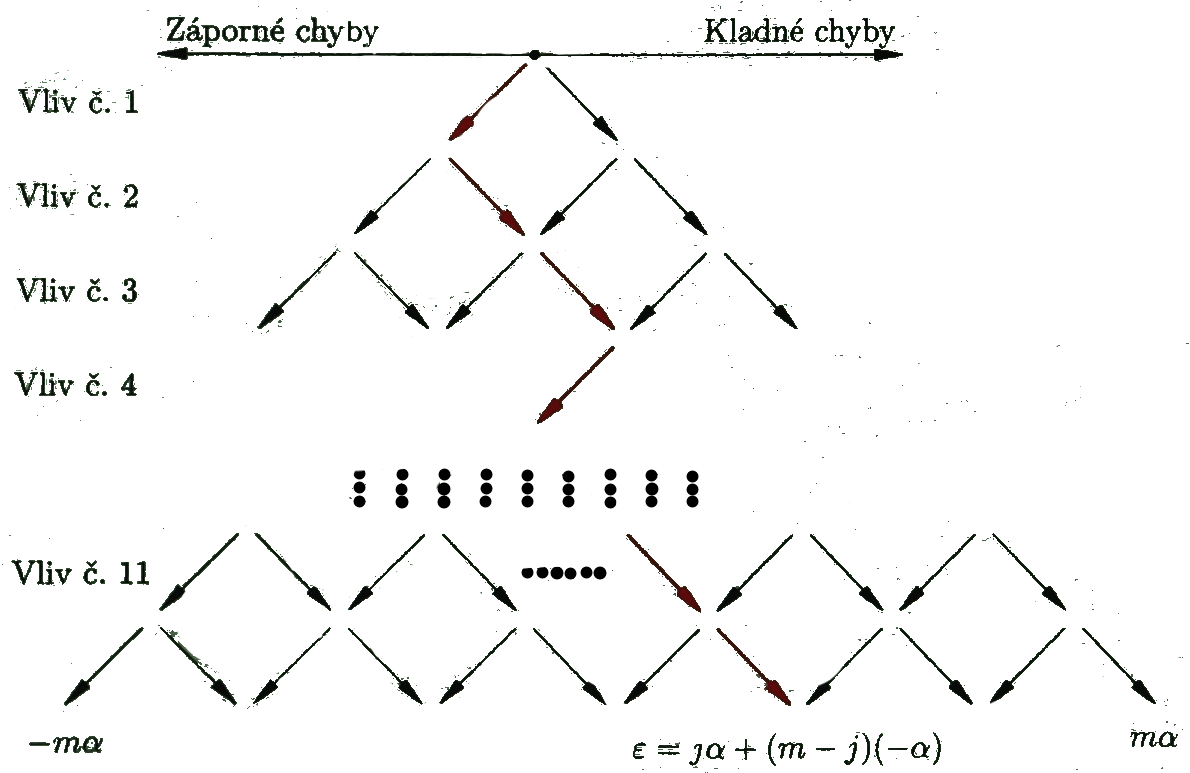
\includegraphics[width=0.6\linewidth]{mai_fig050.png}
        \caption{Vznik kladných a záporných odchylek při měření s \(m\) vlivy. 
        \cite[s.~255]{Musilova2009MA1}}
        \label{mai:fig050}
      \end{figure}
      
      Mohlo by tomu být i naopak, slova „zdar“ a „nezdar“ zde nemají svůj obvyklý význam, jde
      pouze o to, že díky nim můžeme hned uvidět souvislost s Bernoulliovým pokusem a tedy
      i s Bernoulliovým rozdělením. Při \(j\) kladných a \(m — j\) záporných odchylkách je měření od
      správné hodnoty odkloněno o
      \begin{equation*}
        j\alpha + (m - j)(-\alpha) = (2j - m)\alpha
      \end{equation*}
      s pravděpodobností
      \begin{equation*}
        p_j = \begin{pmatrix}m j\end{pmatrix}p^j(1 - p)^{m - j} = 2^{-m}.
      \end{equation*}
      Střední hodnota náhodné veličiny \(\varepsilon\) je nulová. Skutečně, v příkladu 
      \ref{mai:exam066} jsme zjistili, že střední hodnota veličiny \(Y\) nabývající hodnot \(y_j = 
      j\) s Bernoulliovým rozdělením je \(\langle y \rangle = mp\), střední hodnota veličiny \((2j 
      — m)\) a pak musí být \((2mp — m)\alpha\). Pro \(p = \num{0.5}\) je tato hodnota nulová.
      Pro velká \(m\) lze Bernoulliovo rozdělení nahradit rozdělením normálním (obr. 3.8), a proto 
      má náhodná veličina \(\varepsilon\) hustotu pravděpodobnosti tvaru (\ref{mai:eq069}), tj.
      \begin{equation*}
        \mathcal{w}(\varepsilon) = 
        \dfrac{1}{\sigma\sqrt{2\pi}}\exp\left(\dfrac{-\varepsilon^2}{2\sigma^2}\right).   
      \end{equation*}
      \begin{figure}[ht!] %\ref{mai:fig051}
        \centering
        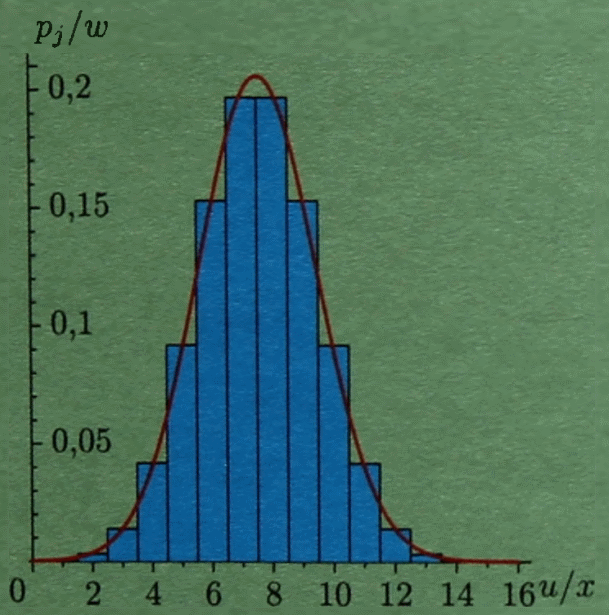
\includegraphics[width=0.4\linewidth]{mai_fig051.png}
        \caption{Normální rozdělení jako limitní případ Bernoulliova 
        \cite[s.~256]{Musilova2009MA1}}
        \label{mai:fig051}
      \end{figure}
      
      Vraťme se nyní k otázce zpracování naměřených hodnot \(\lbrace x_1, \ldots, x_n\rbrace\) 
      výšky válečku. Jejich odchylky od správné hodnoty jsou \(x_1 - x\) až \(x_n - x\). Na místě 
      neznámé správné hodnoty \(x\) si nyní představme nějakou proměnnou, označme ji 
      \(\varepsilon\). Budeme se snažit určit její hodnotu \(\varepsilon_0\) tak, aby 
      pravděpodobnost, že odchylky jednotlivých měřených hodnot od \(\varepsilon_0\) padnou 
      současně do intervalů
      \begin{equation*}
        \left(\varepsilon_1 - \dfrac{\dd{\varepsilon_1}}{2}, 
              \varepsilon_1 + \dfrac{\dd{\varepsilon_1}}{2}
        \right),
        \left(\varepsilon_2 - \dfrac{\dd{\varepsilon_2}}{2}, 
              \varepsilon_2 + \dfrac{\dd{\varepsilon_2}}{2}
        \right), \cdots,
        \left(\varepsilon_n - \dfrac{\dd{\varepsilon_n}}{2}, 
              \varepsilon_n + \dfrac{\dd{\varepsilon_n}}{2}
        \right),
      \end{equation*}
      byla maximální. Pro tuto pravděpodobnost v závislosti na \(\xi\) platí
      \begin{align}
        \dd{W} &= \dd{\mathcal{w}(\varepsilon_1)}\cdots\dd{\mathcal{w}(\varepsilon_n)}  \nonumber\\
               &= \dfrac{1}{\sigma\sqrt{2\pi}}
                  \exp\left(-\dfrac{(x_1 - \xi)^2 + \cdots + (x_n - \xi)^2}{2\sigma^2}
                      \right)\dd{\varepsilon_1}\cdots\dd{\varepsilon_n}.      \label{mai:eq072}
      \end{align}
      (Víte proč je ve vztahu (\ref{mai:eq072}) součin pravděpodobností?) Tato pravděpodobnost bude 
      maximální, bude-li hodnota exponentu minimální. Z podmínky
      \begin{equation*}
        (x_1 - \xi)^2 + \cdots + (x_n - \xi)^2 = \text{min}
      \end{equation*}
      dostáváme derivací podle \(\xi\) požadavek
      \begin{equation*}
        2(x_1 - \xi) + \cdots + 2(x_n - \xi) = 0 \Rightarrow \xi_0 = 
        \dfrac{1}{n}\sum_{i=1}^{n}x_j = \langle x \rangle.
      \end{equation*}
      Vidíme, že veličina, která charakterizuje míru odchýlení naměřených hodnot od \(\xi\), je 
      minimální, zvolíme-li za \(\xi\) aritmetický průměr naměřených hodnot. Pozor, zjištěný 
      výsledek znamená právě jen konstatovanou skutečnost: Při dosazení aritmetického průměru za 
      proměnnou \(\xi\) bude pravděpodobnost, že odchylky jednotlivých měření od \(\xi\) budou 
      ležet v uvažovaných intervalech, maximální. Neznamená to, že správnou hodnotou veličiny \(X\) 
      je aritmetický průměr měření \(x_1, X_2, \ldots, x_n\). Správnou hodnotu ze souboru měření 
      prostě nezjistíme, avšak aritmetický průměr je jí blízký s vysokou pravděpodobností. Jaká je 
      tato „blízkost“ a její pravděpodobnost konkrétně? Hned uvidíme. Správnou hodnotu výšky 
      válečku \(x\) sice neznáme, ale víme, že náhodná veličina \(\varepsilon\), jejíž hodnoty jsou 
      odchylkami výsledků měření od této (neznámé) správné hodnoty, se řídí normálním rozdělením s 
      nulovou střední hodnotou. Potřebujeme stanovit další důležitý parametr tohoto rozdělení, 
      směrodatnou odchylku \(\sigma\). Tu lze vyjádřit velmi jednoduše. Je totiž střední hodnotou 
      náhodné veličiny \(\varepsilon^2\), tedy aritmetickým průměrem čtverců odchylek 
      \(\varepsilon_i\): 
      \begin{equation*}
        \sigma^2 = D(\varepsilon) = \dfrac{1}{n}\sum_{i=1}^{n}\varepsilon_i^2.
      \end{equation*}
      Ať je však tento vzorec jakkoli jednoduchý, k čemu může sloužit, nedokážeme-li jej vyčíslit?
      Když přece neznáme správnou hodnotu \(x\), nemáme k dispozici ani hodnoty \(\varepsilon_i\). 
      Ani tato kaše však není tak horká, jak se zdá: Odchylku výsledku \(i\)-tého měření od 
      aritmetického průměru označme \(\delta_i = x_i - \langle x \rangle\), přičemž jsme již dříve 
      označili jako \(\varepsilon_i= x_i - x\) odchylku výsledku \(i\)-tého měření pd správné 
      hodnoty. Platí
      \begin{equation*}
        \sum_{i=1}^{n}\varepsilon_i = \sum_{i=1}^{n}(x_i - x) \Rightarrow 
        \sum_{i=1}^{n}x_i = \sum_{i=1}^{n}\varepsilon_i + nx, 
      \end{equation*}
      odkud 
      \begin{equation*}
        \langle x \rangle = x + \dfrac{1}{n}\sum_{i=1}^{n}\varepsilon_i.
      \end{equation*}
      Pak dostaneme
      \begin{equation*}
        \delta_i = (x_i - x) - \dfrac{1}{n}\sum_{i=1}^{n}\varepsilon_i 
                 = \varepsilon_i - \dfrac{1}{n}\sum_{j=1}^{n}\varepsilon_j.
      \end{equation*}
      Součet čtverců odchylek \(\delta_i\) je
      \begin{align*}
        \sum_{i=1}^{n}\delta_i^2 
          &= \sum_{i=1}^{n}\left(\varepsilon_i - 
             \dfrac{1}{n}\sum_{j=1}^{n}\varepsilon_j\right)^2 = \sum_{i=1}^{n}\varepsilon_i^2 - 
             \dfrac{2}{n}\sum_{i=1}^{n}\sum_{j=1}^{n}\varepsilon_i\varepsilon_j + 
             \dfrac{1}{n^2}\sum_{i=1}^{n}\left(\sum_{j=1}^{n}\varepsilon_j\right)^2     \\
          &= \sum_{i=1}^{n}\varepsilon_i^2 - 
             \dfrac{1}{n}\left(\sum_{j=1}^{n}\varepsilon_j\right)^2                     
             \doteq \left(1 - \dfrac{1}{n}\right)\sum_{i=1}^{n}\varepsilon_i^2.
      \end{align*}
      Při poslední úpravě jsme pro získání výsledného přibližného vyjádření součtu čtverců odchylek
      \(\delta_i\) použili následující úvahy:
      \begin{equation*}
        \left(\sum_{j=1}^{n}\varepsilon_j\right)^2 = \sum_{i=1}^{n}\varepsilon_i^2 + 
        2\sum_{i=1}^{n}\sum_{j>1}\varepsilon_i\varepsilon_j \doteq \sum_{i=1}^{n}\varepsilon_i^2,
      \end{equation*}
      neboť při rovnocenném zastoupení kladných a záporných odchylek je druhý sčítanec, obsahující
      součiny \(\varepsilon_i\varepsilon_j\), zanedbatelný proti prvnímu. Nakonec tedy dostáváme
      \begin{equation*}
        \sum_{i=1}^{n}\delta_i^2 \doteq \dfrac{n-1}{n}\sum_{i=1}^{n}\varepsilon_i^2 = (n-1)\sigma^2.
      \end{equation*}
      Protože odchylky \(\delta_i\) již z daného souboru měření určit můžeme (jsou to odchylky 
      jednotlivých měření od jejich aritmetického průměru), získali jsme alespoň přibližný vztah 
      pro směrodatnou odchylku rozdělení veličiny \(\varepsilon\), 
      \begin{equation}\label{mai:eq074}
        \sigma = \left(\dfrac{1}{n-1}\sum_{i=1}^{n}\delta_i^2\right)^{\dfrac{1}{2}}.
      \end{equation}
      Jaký význam má tato hodnota pro náš soubor měření? Vymezuje interval
      \begin{equation*}
        (x - \sigma, x + \sigma),
      \end{equation*}
      symetrický kolem (stále neznámé) správné hodnoty výšky válečku \(x\), do kterého padne 
      výsledek měření této výšky s pravděpodobností \SI{68.3}{\percent} (příklad 
      \ref{mai:exam069}). Neznámá správná hodnota je tedy naopak s toutéž pravděpodobností vzdálena 
      od výsledku jednotlivého měření o méně než \(\sigma\). A to už je docela slušná informace o 
      tom, kde správná hodnota může ležet. Polohu \(x\) však můžeme „omezit“ ještě lépe. Směrodatná 
      odchylka \(\overline{\sigma}\) rozdělení, které přísluší aritmetickému průměru, je
      totiž ještě \(\sqrt{n}\)-krát menší než \(\sigma\), tj. \(\overline{\sigma}= 
      \sigma/\sqrt{n}\). Správná hodnota \(x\) (navždy neznámá) je tedy od aritmetického průměru 
      výsledků měření \(\langle x \rangle\) vzdálena s pravděpodobností \SI{68.3}{\percent} o méně 
      než \(\overline{\sigma}\). Použijeme-li krajní chybu \(\overline{\kappa} = 
      3\overline{\sigma}\) (příklad \ref{mai:exam069}), můžeme říci, že správná hodnota \(x\) je od
      aritmetického průměru souboru měření \(\langle x \rangle\) vzdálena o méně než 
      \(\overline{\kappa}\) s pravděpodobností \SI{99.7}{\percent}. Více se o správné hodnotě výšky 
      válečku říci nedá. Ale i tak jsme ji lokalizovali docela úspěšně. Následující příklad 
      ukazuje vyhodnocení konkrétního souboru měření.

      %-- Měříme výšku válečku----------------------------------------
      % !TeX spellcheck = cs_CZ
\begin{mdframed}[style=mdexam]
  \begin{example}\label{mai:exam077}
    \textbf{Měříme výšku válečku}\newline
    Student měřil za stejných podmínek výšku válečku dvacetkrát. Při měření byly vyloučeny
    systematické chyby. Měřil tentokrát přesněji - posuvným měřítkem neboli „šuplérou“. Mohl tedy
    odhadovat desetiny milimetru. Získal tyto hodnoty \(x_1\) až \(X_{20}\) v milimetrech (levá část
    tabulky):
    
    {\centering
      \resizebox{\textwidth}{!}{%
      \begin{tabular}{c|ccccc|ccccc}
        \hline
        měření & \multicolumn{5}{l}{\(x_i\) [mm]} & \multicolumn{5}{l}{\(\delta_i\) [mm]} \\ \hline
        1.  až 5.  & \num{35.5} & \num{35.4} & \num{34.9} & \num{35.7} &
                  \num{36.0} & \num{0.2}  & \num{0.1}  & \num{-0.4} & \num{0.4}
                  & \num{0.7}     \\
        6.  až 10. & \num{35.8} & \num{35.2} & \num{35.2} & \num{34.8} &
                  \num{35.0} & \num{0.5}  & \num{-0.1} & \num{-0.1} & \num{-0.5}
                  & \num{-0.3}    \\
        11. až 15. & \num{35.5} & \num{34.8} & \num{35.1} & \num{35.3} &
                  \num{34.9} & \num{0.2}  & \num{-0.5} & \num{-0.2} & \num{0.0}
                  & \num{-0.4}    \\
        16. až 20. & \num{35.8} & \num{35.4} & \num{35.8} & \num{34.8} &
                  \num{35.1} & \num{0.5}  & \num{0.1}  & \num{0.5}  & \num{-0.5}
                  & \num{-0.2}    \\ \hline
      \end{tabular}}
    \par}
    \vspace{\baselineskip}
    Aritmetický průměr těchto hodnot je \(\langle x\rangle = \qty{35.30}{\mm}\). Uvádíme jej zatím s
    přesností o jedno desetinné místo „lepší“ , než jsou jednotlivá měření, neboť ještě nevíme, jak
    dopadnou výpočty chyb. V pravé části tabulky jsou hodnoty \(\delta_i\), tj. odchylky
    jednotlivých měření od aritmetického průměru. Snadno se přesvědčíme, že jejich součet je nulový,
    přesně, jak má být. Směrodatná odchylka vychází \(\sigma \doteq \qty{0.381}{\mm}\) pro jednotlivé
    měření, pro aritmetický průměr pak \(\overline{\sigma} \doteq \qty{0.085}{\mm}\). Na rozdíl od
    hodnot měření se výsledné chyby měření zaokrouhlují vždy nahoru, a to na jedno platné místo.
    (Zaokrouhlujeme nahoru proto, abychom zajistili, že správná hodnota veličiny leží v intervalu
    určeném chybou nejméně s pravděpodobností, která této chybě odpovídá. Po zaokrouhlení tedy máme
    \(\sigma \doteq \qty{0.4}{\mm}\) a \(\overline{\sigma} = \qty{0.09}{\mm}\). Změřenou výšku válečku
    pak zapisujeme takto:
    \begin{equation*}
      \text{výška válečku } = (\langle x \rangle\pm \overline{\sigma}) = \qty{35.30 \pm 0.09}{\mm}.
    \end{equation*}
    Z předchozích úvah víme, jak je nutno takový zápis interpretovat:
    \begin{itemize}
      \item Správná hodnota výšky válečku leží v intervalu \SIrange[range-units =
            brackets]{35.21}{35.39}{\mm} a pravděpodobností nejméně \qty{68.3}{\percent}.
    \end{itemize}
    Při použití krajní chyby, tj. \(\overline{\kappa} \doteq \qty{0.27}{\mm} \doteq \qty{0.3}{\mm}\),
    konstatujeme, že
    \begin{itemize}
      \item Správná hodnota výšky válečku leží v intervalu \SIrange[range-units =
            brackets]{35.0}{35.6}{\mm} s pravděpodobnosti nejméně \qty{99.7}{\percent}.
    \end{itemize}
    Pozn.: Při zcela korektním přístupu ke zpracování laboratorních měření je třeba uvážit, že
    intervaly se stejným pravděpodobnostním obsahem \qty{68.3}{\percent}, resp. \qty{99.7}{\percent}
    jsou ve skutečnosti širší. Správně by totiž měly být stanoveny na základě nekonečného počtu
    měření
  \end{example}
\end{mdframed}
      %---------------------------------------------------------------
      Na závěr odstavce si všimneme ještě jedné důležité otázky. Formulujeme ji pro případ určení
      hustoty válečku. Změřili jsme výšku válečku \(x\) a jeho poloměr \(r\), vážením jsme určili 
      také jeho hmotnost \(m\). Získali jsme tak intervaly
      \begin{equation*}
        \left(\langle x \rangle - \overline{\sigma}(x), 
              \langle x \rangle + \overline{\sigma}(x)\right), \qquad
        \left(\langle r \rangle - \overline{\sigma}(r), 
              \langle r \rangle + \overline{\sigma}(r)\right), \qquad
        \left(\langle m \rangle - \overline{\sigma}(m), 
              \langle m \rangle + \overline{\sigma}(m)\right).
      \end{equation*}
      
      Směrodatná odchylka v případě každé z veličin \(x\), \(r\) a \(m\) určuje velikost intervalu 
      se středem daným aritmetickým průměrem všech měření této veličiny, v němž leží správná 
      hodnota s pravděpodobností \SI{68.3}{\percent}. Průměrná hustota válečku je dána vztahem
      \begin{equation*}
        \varrho = \dfrac{m}{V} = \dfrac{m}{\pi r^2x},
      \end{equation*}
      je tedy funkcí tří proměnných \(x\), \(r\), \(m\). Jak stanovíme interval, v němž leží 
      správná hodnota hustoty s pravděpodobností rovněž \SI{68.3}{\percent}? Hustotu totiž neměříme 
      přímo, ale vypočítáváme z přímo měřených veličin. Abychom mohli na tuto otázku odpovědět 
      matematicky korektně, potřebujeme základní znalosti o funkcích více proměnných. Závěr tohoto 
      odstavce lze tedy do důsledku pochopit po přečtení kapitoly o funkcích více proměnných. Proto 
      jej v tuto chvíli klidně přeskočte.
      
      Předpokládejme, že veličina \(z\) je pro jednoduchost pouze funkcí dvou nezávislých náhodných
      veličin \(x\) a \(y\), \(z = f(x,y)\). Jsou-li chyby \(\varepsilon_i(x)\), resp. 
      \(\varepsilon_i(y)\), kterých jsme se dopustili při \(i\)-tém měření veličiny \(x\), resp. 
      \(y\) velmi malé, můžeme pro vyjádření malé změny veličiny \(z\) způsobené chybami veličin 
      \(x\) a \(y\) použít úplného diferenciálu
      \begin{equation*}
        \dd{z} = \dd{f(x,y)} = \left(\pder{f(x,y)}{x}\right)\dd{x} + 
                               \left(\pder{f(x,y)}{y}\right)\dd{y}
      \end{equation*}
      Pro chybu veličiny \(z\) pak platí
      \begin{equation*}
        \varepsilon_i(z) = \left(\pder{f}{x}\right)\varepsilon_i(x) + 
                           \left(\pder{f}{y}\right)\varepsilon_i(y) \Rightarrow
      \end{equation*}
      \begin{equation*}
        \Rightarrow \sum_{i=1}^{n}\varepsilon_i^2(z) 
        =  \sum_{i=1}^{n}\left(\pder{f}{x}\right)^2\varepsilon_i^2(x) 
        +  \sum_{i=1}^{n}\left(\pder{f}{y}\right)^2\varepsilon_i^2(y)
        + 2\sum_{i=1}^{n}\left(\pder{f}{x}\right)^2\left(\pder{f}{y}\right)^2\varepsilon_i(x)
          \varepsilon_i(y).
      \end{equation*}
      Vzhledem k rovnocennému zastoupení kladných a záporných odchylek je součet obsahující
      součiny \(\varepsilon_i(x)\varepsilon_i(y)\) zanedbatelný proti zbytku výrazu. Pak
      \begin{equation*}
        \sum_{i=1}^{n}\varepsilon_i^2(z) \doteq \left(\pder{f}{x}\right)^2
        \sum_{i=1}^{n}\varepsilon_i^2(x) + 
                      \left(\pder{f}{y}\right)^2\sum_{i=1}^{n}\varepsilon_i^2(y) 
        = \left(\pder{f}{x}\right)^2 n\sigma^2(x) + \left(\pder{f}{y}\right)^2n\sigma^2(y).
      \end{equation*}
      Odtud, vzhledem k platnosti vztahu
      \begin{equation*}
        \sum_{i=1}^{n}\varepsilon_i^2 = n\sigma^2(z),
      \end{equation*}
      dostáváme
      \begin{equation}\label{mai:eq075}
        \sigma^2(z) = \left(\pder{f}{x}\right)^2\sigma^2(x)
                    + \left(\pder{f}{y}\right)^2\sigma^2(y).
      \end{equation}
      Parciální derivace funkce \(f(x, y)\) podle \(x\), resp. \(y\) je třeba vyčíslit dosazením 
      \(x = \langle x\rangle\) a \(y = \langle y \rangle\). Zobecnění tohoto vzorce na případ, kdy 
      hledaná veličina je funkcí více proměnných, je jednoduché.
      
    \subsection{Lineární závislost a metoda nejmenších čtverců}
      Tento poslední odstavec se zabývá zpracováním měření veličin, které jsou vázány lineárním
      vztahem (už zase ta linearita). Situaci si opět snadno představíme na jednoduchém příkladu
      Víme, že pro elektrické vodiče platí za jistých okolností \emph{Ohmův zákon}. Podle něj je 
      proud \(I\) protékající vodičem, třeba drátem, přímo úměrný napětí \(U\) mezi konci vodiče. 
      Konstanta úměrnosti ve vztahu
      \begin{equation*}
        U = R\cdot I
      \end{equation*}
      představuje \emph{elektrický odpor vodiče} \(R\). Změříme-li napětí a proud, můžeme určit 
      odpor vodiče, pokud Ohmův zákon opravdu platí. Mohli bychom tedy postupovat například tak, že 
      bychom při několika různých hodnotách napětí \(\lbrace U_1, U_2, \ldots, U_n \rbrace\) 
      (napětí bychom mohli například postupně zvyšovat) změřili proud protékající vodičem, tj. 
      \(\lbrace I_1, I_2, \ldots, I_n \rbrace\), a určili odpovídající hodnoty odporu \(R_1 = 
      U_1/I_1\), \(R_2 = U_2/I_2\), \(\ldots\), \(R_n = U_n/I_n\)  Protože by měřené hodnoty napětí 
      i proudu byly ovlivněny náhodnými vlivy a byly tak zatíženy chybami, byly by získané hodnoty 
      odporu obecně různé, i když blízké. Zpracovali bychom je podobně jako soubor \(\langle x_1, 
      x_2, \ldots, x_n \rangle\) při měření výšky válečku. Co když ale Ohmův zákon neplatí? Máme-li 
      k dispozici změřený soubor odpovídajících si hodnot napětí a proudu, můžeme Ohmův zákon pro 
      daný případ dokonce ověřit. Nebudeme však z jednotlivých údajů \(U_i\) a \(I_i\) počítat 
      hodnoty \(R_i\) a pak je průměrovat, ale zpracujeme celý soubor měření „najednou“. Představme 
      si dvojice \([U_i, I_i]\) jako body grafu. Kdyby měření napětí ani proudu nebyla zatížena 
      chybami a kdyby přesně platil Ohmův zákon, ležely by body grafu přesně na přímce. Odpor 
      vodiče bychom pak, s uvážením jednotek na osách, určili jako její směrnici (resp. v našem 
      případě, kdy na vodorovnou osu nanášíme napětí a na svislou osu proud, je směrnicí převrácená 
      hodnota odporu). Pro každou dvojici odpovídajících si hodnot napětí a proudu by mělo platit
      \begin{equation*}
        U_1 = R\cdot I_1, U_2 = R\cdot I_2, \ldots, U_n = R\cdot I_n.
      \end{equation*}
      Předchozí zápis můžeme chápat jako nehomogenní soustavu \(n\) lineárních rovnic pro jedinou
      neznámou \(R\). Rozšířená matice této soustavy je
      \begin{equation*}
        \overline{B} = (A|B) = 
          \left(
            \begin{array}{c|c}
              I_1    & U_1     \\
              I_2    & U_2     \\
              \cdots & \cdots  \\
              \cdots & \cdots  \\
              I_n    & U_n
            \end{array}
          \right).
      \end{equation*}
      Matice soustavy \(A\) má hodnost \(h(A) = 1\), matice \(\overline{B} = (A|B)\) však bude mít 
      vlivem chyb měření hodnost \(h(\overline{B}) = 2\). Soustava tedy obecně nemá řešení. Je 
      „přeučena“, neboť máme více nezávislých rovnic a jen jednu neznámou. Přímku, která by 
      procházela všemi body grafu, nenajdeme. Položíme si proto splnitelný úkol: Budeme hledat 
      přímku, která by se co „nejlépe přimykala“ k souboru bodů grafu. Tento požadavek je třeba 
      matematicky formulovat, jinak bude k nepotřebě. Označme hledanou hodnotu odporu \(R\). Pokud 
      by hodnoty \(\lbrace I_1, I_2, \ldots, I_n \rbrace\) byly bezchybné, odpovídaly by jim 
      hodnoty napětí \(\lbrace R_1\cdot I_1, R_2\cdot I_2, \ldots, R_n\cdot I_n \rbrace\). Odchylky 
      skutečně naměřených napětí \(\lbrace U_1, U_2, \ldots, U_n \rbrace\) od těchto „teoretických“ 
      jsou
      \begin{equation*}
        \lbrace U_1 - R_1\cdot I_1, U_2 - R_2\cdot I_2, \ldots, U_n - R_n\cdot I_n \rbrace.
      \end{equation*}
      Součet jejich čtverců je funkcí veličiny \(R\), kterou na chvíli považujme za proměnnou:
      \begin{equation*}
        D(R) = \sum_{i = 1}^{n}(U_i - R_i\cdot I_i)^2.
      \end{equation*}
      Řekneme, že se přímka o rovnici \(U = R\cdot I\) nejlépe přimyká k souboru bodů \(\lbrace[ 
      U_i, I_i]\rbrace\) právě tehdy, je-li \(R\) zvoleno tak, aby hodnota \(D(R)\) byla co 
      nejmenší. Nutnou podmínkou pro minimum funkce \(D(R)\) je nulovost její derivace,
      \begin{equation*}
        \der{D(R)}{R} = -2\sum_{i = 1}^{n}(U_i - R_i\cdot I_i)I_i = 0,
      \end{equation*}
      odkud
      \adjustbox{minipage=[c]{\textwidth}}{%
        \begin{equation}\label{mai:eq073}
          R=  \dfrac{\sum_{i = 1}^{n}U_i\cdot I_i}{\sum_{i = 1}^{n}I_i^2}.
        \end{equation}
      }
      Předchozím vztahem je určena hodnota odporu. Jejím dosazením do vzorce pro \(D(R)\) zjistíme
      odpovídající odchylku
      \adjustbox{minipage=[c]{\textwidth}}{%
        \begin{equation*}
          \sigma(R) = \sqrt{\dfrac{D(R)}{n-1}}.
        \end{equation*}
      }
      Velikost \(\sigma(R)\) dává informaci o tom, jak „dobře“ vyhovuje testovaný soubor měření 
      zvolenému fyzikálnímu modelu, v tomto případě lineární závislosti.

      %-- Ověření Ohmová zákona---------------------------------------
      % !TeX spellcheck = cs_CZ
% \wikitextrule
\begin{mathexam}{Ověření Ohmová zákona}{exam076}
  Naměřili jsme následující hodnoty napětí na vodiči a jim odpovídající hodnoty proudu:
  
  \begin{center}
    \resizebox{1\textwidth}{!}{%
    \begin{tabular}{ccc|ccc}
      \hline
      měření & napětí [V] & proud [A]  & měření & napětí [V] & proud [A]    \\
      \hline
      1.     & \num{2.45} & \num{0.70} & 7.     & \num{7.42} & \num{2.17}   \\
      2.     & \num{4.33} & \num{1.22} & 8.     & \num{7.87} & \num{2.21}   \\
      3.     & \num{5.39} & \num{1.54} & 9.     & \num{8.14} & \num{2.34}   \\
      4.     & \num{5.76} & \num{1.66} & 10.    & \num{8.67} & \num{2.51}   \\
      5.     & \num{6.62} & \num{1.89} & 11.    & \num{9.12} & \num{2.53}   \\
      6.     & \num{7.05} & \num{2.00} & 12.    & \num{9.85} & \num{2.76}   \\
      \hline
    \end{tabular}}
  \end{center}

  {\centering
  \captionsetup{type=figure}
  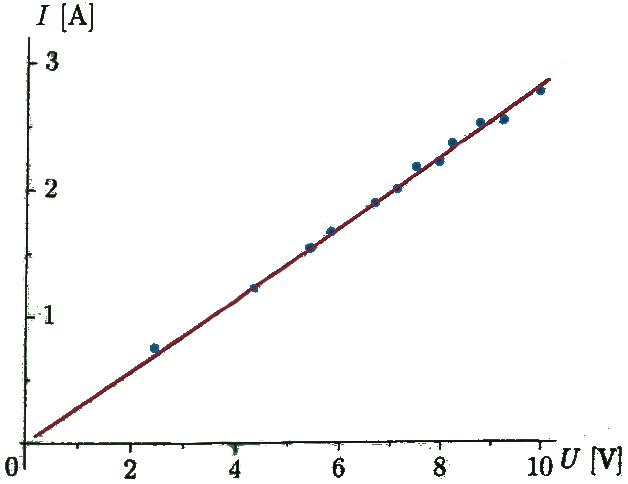
\includegraphics[width=0.8\linewidth]{mai_fig052.png}
  \captionof{figure}{Ověření Ohmová zákona lineární regresí.
  \cite[s.~263]{Musilova2009MA1}
  \label{mai:fig052}}
  \par}
  Pro odpor vychází \(R\doteq\SI{3.52}{\ohm}\). Součet čtverců odchylek přímky se směrnicí \(i/R
  = (1/\num{3.52})\Omega^{-1}\) od souboru bodů grafu je
  \begin{equation*}
    D(R) = \sum_{i=1}^{n}(U_i - R\cdot I_i)^2 \doteq\num{0.01},
  \end{equation*}
  \(\sigma(R) = \sqrt{D(R)/(n-1)}\doteq\sqrt{(\num{0.11}/11)}\doteq\num{0.03}\).  Graf přímky \(U
  = R\cdot I = \num{3.52}\cdot I\) proložené body je na obrázku \ref{mai:fig052}.
\end{mathexam}
      %---------------------------------------------------------------
      
      Popsaný způsob nalezení hodnoty elektrického odporu vodiče se nazývá\textbf{ metodou 
      nejmenších čtverců} (minimalizuje součet čtverců odchylek prokládané závislosti od souboru 
      naměřených bodů), v případě použití lineárního modelu, jako tomu bylo u Ohmová zákona, pak 
      jde o \textbf{lineární regresi}
      
      Obdobně se postupuje, je-li některá z měřených veličin lineární funkcí veličin jiných s 
      neznámými koeficienty lineární kombinace. Nechť
      \begin{equation*}
        Z = f(X_1, X_2, \ldots, X_K) = A_1X_1 + A_2X_2 + \cdots + A_KX_K.
      \end{equation*}
      Předpokládejme, že veličiny \(X_1, X_2, \ldots, X_K\) a \(Z\) měříme \(n\)-krát a naměříme 
      hodnoty
      \begin{equation*}
        X_j = \lbrace x_{j1}, \ldots x_{jn} \rbrace, \qquad 1 \leq j \leq K, \qquad 
        Z = \lbrace z_{1}, \ldots z_{n} \rbrace
      \end{equation*}
      Součet čtverců odchylek teoretické závislosti od naměřených bodů je
      \begin{equation*}
        D(Z) = \sum_{i=1}^{n}\left(z_i - \sum_{j=1}^{K}A_jx_{ji}\right)^2.
      \end{equation*}
      Nutnou podmínkou pro minimum tohoto výrazu jakožto funkce proměnných \(A_x, A_2, \ldots, A_K\)
      je platnost souboru rovnic
      \begin{equation*}
        \pder{D(Z)}{A_p} = 0 \Rightarrow 
        \sum_{i=1}^{n}2\left(z_i - \sum_{j=1}^{K}A_jx_{ji}\right)\cdot x_{pi} = 0
      \end{equation*}
      pro \(1 \leq i \leq n, 1 \leq j \leq K\). Tyto podmínky představují nehomogenní soustavu 
      \(K\) rovnic pro \(K\) neznámých \(( A_1, A_2, \ldots, A_K)\). Rozšířená matice soustavy je
      \begin{equation*}
        \overline{B} = (A|B) = 
          \left(
            \begin{array}{cccc|c}
              \sum_{i=1}^{n}x_{1i}x_{1i} & \sum_{i=1}^{n}x_{1i}x_{2i} & \cdots & 
              \sum_{i=1}^{n}x_{1i}x_{Ki} & \sum_{i=1}^{n}z_{i}x_{1i}                    \\
              \sum_{i=1}^{n}x_{1i}x_{1i} & \sum_{i=1}^{n}x_{2i}x_{2i} & \cdots & 
              \sum_{i=1}^{n}x_{2i}x_{Ki} & \sum_{i=1}^{n}z_{i}x_{2i}                    \\
                        \cdots           & \cdots & \cdots & \cdots   & \cdots          \\
              \sum_{i=1}^{n}x_{Ki}x_{1i} & \sum_{i=1}^{n}x_{Ki}x_{2i} & \cdots & 
              \sum_{i=1}^{n}x_{Ki}x_{Ki} & \sum_{i=1}^{n}z_{i}x_{Ki}                    \\
            \end{array}
          \right),
      \end{equation*}
      \begin{equation*}
        \sigma(z) = \sqrt{\dfrac{D(z)}{n - K}}.
      \end{equation*}
      V dalších kapitolách věnovaných lineární algebře se k tomuto problému znovu vrátíme a 
      ukážeme, že jej lze elegantně řešit také jako úlohu algebraickou, konkrétně úlohu o 
      ortogonální projekci vektorů na podprostory.
      
%} %tikzset
%---------------------------------------------------------------------------------------------------
\printbibliography[heading=subbibliography]
\addcontentsline{toc}{section}{Seznam literatury}
%--------------------- Kombinatorika, pravděpdobnost, statistika ----------------------------------
  % !TeX program = lualatex 
% !TeX root = luaking.tex 
% !TeX encoding = UTF-8 
% !TeX spellcheck = cs_CZ
 %---------------------------------------------------------------------------------------------------
\graphicspath{{../src/MAI/img/}}
% file mai1ch04c.tex
%---------------------------------------------------------------------------------------------------
\setchaptertoc
\chapter{Kombinatorika}\label{mai:IchapIVc}
  \textbf{Kombinatorika} se od všech matematických disciplín, v několika směrech liší. Zatímco v
  geometrii má každá přímka nekonečnou délku a každý trojúhelník nekonečně mnoho bodů, zatímco v
  algebře některé rovnice i nerovnice mají nekonečně mnoho řešení a zatímco matematická analýza
  zkoumá limity posloupností a funkcí, roste-li příslušná proměnná do nekonečna, v kombinatorice se
  s nekonečnem nesetkáme. Kombinatorika je součástí \textbf{finitní matematiky}, která studuje
  konečné soubory (množiny a uspořádané \(k\)-tice, \(k\in \mathcal{N}\)). 
  
  Další odlišností je to, že často nemáme možnost ověřit si správnost výsledku, ke kterému jsme při
  řešení kombinatorické úlohy dospěli, a jsme odkázáni jen na svůj vlastní úsudek. Proto v
  kombinatorice v míře větší než jinde platí, že „cvičení dělá mistra“. 
  
  V této kapitole je probrána část kombinatoriky, která se zabývá vytvářením skupin z daných prvků a
  určováním jejich počtu. Jde o klasickou problematiku, která byla řešena již v 17. a 18. století a
  která je spojena se jmény \emph{B. Pascala}, \emph{P. Fermata}, \emph{J Bernoulliho}, \emph{G. W.
  Leibnize}  a \emph{L. Eulera}. Dnes představuje kombinatorika rozsáhlou matematickou disciplínu,
  některé její problémy byly již vyřešeny (problém čtyř barev) mnohé další na své vyřešení čekají. 
  
  A závěrem ještě důležitá poznámka terminologická: přirozenými čísly se v této kapitole rozumějí
  čísla celá kladná tj. čísla 1, 2, 3, 4, \(\ldots\), nula se tedy mezi přirozená čísla nezahrunuje.
  \cite[s.~7]{calda2008matematika} 
    
  \twocolumn[\section{Základní kombinatorická pravidla}\label{mai:IchapIVcsecI}]
    K řešení velké části kombinatorických úloh vystačíme s dvěma jednoduchými pravidly. Je dost
    pravděpodobné, že jsme je už sami několikrát použili, aniž nám bylo známo, že se o nějaká
    kombinatorická pravidla vůbec jedná. Vysvětlíme si je na řešení následujících (velmi snadných
    příkladů).

    %--Počet všech přirozených dvojciferných čísel------------------
    % !TeX spellcheck = cs_CZ
\begin{mdframed}[style=mdexam]
  \begin{example}\label{mai:exam094}
    Pokusme se určit počet všech přirozených dvojciferných čísel, v jejichž dekadickém zápisu se
    každá číslice vyskytuje nejvýše jednou. Kredit: \cite[s.~8]{calda2008matematika} \newline
    \textbf{Řešení}:
    \begin{enumerate}[noitemsep]
      \item způsob: na místě desítek může stát libovolná z devíti číslic \(1, 2, \ldots, 9\), neboť
            zde nesmí být číslice 0. Ke každé z těchto devíti možností pro výběr číslice na místě
            desítek existuje devět možností, jak vybrat číslici pro místo jednotek: může zde totiž
            být číslice 0 a jakákoliv z osmi číslic, která je různá od číslice stojící na místě
            desítek. Počet uvažovaných dvojciferných čísel je tedy \(9\cdot9 = 81\).
      \item způsob: všechna přirozená dvojciferná čísla lze rozložit do dvou disjunktních skupin
            tak, že v první jsou dvojciferná čísla s různými a ve druhé dvojciferná čísla s týmiž
            číslicemi. Je zřejmé, že všech dvojciferných čísel je 90 a dvojciferných čísel s týmiž
            číslicemi 9 ( jde o čísla \(11, 22, \ldots, 99)\); označíme-li \(p\) hledaný počet
            dvojciferných čísel s různými číslicemi, platí \(p+9 = 90\). Odtud dostáváme, že je
            \(p=81\).      
    \end{enumerate}
  \end{example}
\end{mdframed}
    %---------------------------------------------------------------

    V prvním řešení příkladu je obsaženo kombinatorické pravidlo součinu:
    
    \begin{mdframed}[style=highlight] Počet všech uspořádaných \(k\)-tic, jejichž první člen lze
      vybrat \(n_1\) způsoby, druhý člen po výběru prvního členu \(n_2\) způsoby atd. až \(k\)-tý
      člen po výběru všech předcházejících členů \(n_k\) způsoby, je roven \(n_1\cdot n_2\cdots
      n_k\).
    \end{mdframed}

    Vskutku: uvedená dvojciferná čísla lze považovat za uspořádané dvojice s různými členy, protože
    první člen lze vybrat devíti způsoby a druhý (po výběru prvního) rovněž devíti způsoby, je počet
    těchto uspořádaných dvojic - tj. uvažovaných dvojciferných čísel - roven \(9\cdot9= 81\).

    Ve druhém řešení bylo použito kombinatorické pravidlo součtu:
    
    \begin{mdframed}[style=highlight] Jsou-li \(A_1\), \(A_2\), \(\cdots\), \(A_n\) konečné množiny,
      které mají po řadě \(p_1\), \(p_2\), \(\cdots\), \(p_n\) prvků, a jsou-li každé dvě
      disjunktní, pak - počet prvků množiny \(A_1 \cup A_2 \cup\cdots\cup A_n\), je roven \(p_1 +
      p_2 \cdots + p_n\).        
    \end{mdframed}

    Je jasné, že v uvedeném příkladu je \(A_1\) množina všech dvojciferných čísel s různými
    číslicemi a \(A_2\) množina všech dvojciferných čísel s týmiž číslicemi. 
    
    Jak je vidět, jsou obě pravidla téměř samozřejmá, což jim vsak neubírá na významu; pomocí nich
    odvodíme v dalších článcích některé kombinatorické vzorce. V následujícím příkladu uvidíme, jak
    kombinatorické pravidlo součinu může pomoci při rozhodování, kolikrát je vlastně daný objekt (v
    příkladu jde o trojúhelník) počítán.
  
    %--Počet všech trojúhelníků XYZ---------------------------------
    % !TeX spellcheck = cs_CZ
\begin{mdframed}[style=mdexam]
  \begin{example}\label{mai:exam095}
    Je dán čtverec \(ABCD\) a na jeho každé straně n vnitřních bodů. Určete počet všech trojúhelníků
    \(XYZ\), jejichž vrcholy leží v daných bodech a na různých stranách čtverce \(ABCD\). Kredit
    \cite[s.~9]{calda2008matematika}.\newline
    \textbf{Řešení}:
    \begin{itemize}[noitemsep]
      \item Vrchol \(X\) je možno zvolit v libovolném z daných bodů, takže pro něj máme \(4n\)
            způsobů výběru. Po výběru bodu \(X\) lze bod \(Y\) vybrat už jen \(3n\) způsoby, neboť
            nesmí ležet na téže straně čtverce jako bod \(X\).
      \item Po výběru bodu \(Y\) je možné bod \(Z\) vybrat pouze \(2n\) způsoby, neboť nesmí ležet
            na těch stranách čtverce \(ABCD\), na nichž leží body \(X\), \(Y\). Existuje tedy
            \(4n\cdot3n \cdot2n = 24n^3\) uspořádaných trojic utvořených z bodů \(X\), \(Y\), \(Z\).
      \item Uvědomme si však, že šest uspořádáných trojic takto sestavených určuje stejný
            trojúhelník. Tak např. každá z uspořádaných trojic \((X, Y, Z)\), \((X, Z, Y)\), \((Y,
            X, Z)\), \((Y, Z, X)\), \((Z, X, Y),\) \((Z, Y, X)\) představuje trojúhelník, a to
            \(\Delta XYZ\). 
      \item Abychom dostali počet všech trojúhelníků požadované vlastnosti, musíme získaný počet
            uspořádaných trojic dělit šesti. Trojúhelníků dané vlastnosti je tedy:
            \begin{equation*} 
              \dfrac{24n^3}{6}
            \end{equation*}
    \end{itemize}

    {\centering
    \captionsetup{type=figure} 
    \luafigure[0.8]{mai_fig069}
    \captionof{figure}{Ilustace k příkladu \ref{mai:exam095}}
    \label{mai:fig069}
    \par}

  \end{example}
\end{mdframed}
    %---------------------------------------------------------------

    V řešení následujícího \uv{turistického} příkladu jsou použita obě uvedená pravidla. Poznáme jak?
    
    %--Turistický příklad-------------------------------------------
    % !TeX spellcheck = cs_CZ
\begin{mdframed}[style=mdexam]
  \begin{example}\label{mai:exam096}
    Z místa \(A\) do místa \(B\) vedou čtyři turistické cesty, z místa \(B\) do místa \(C\) tři.
    Určete, kolika zpåsoby lze vybrat trasu z \(A\) do \(C\) a zpět tak, že z těchto sedmi cest je
    právě jedna použita dvakrát. \newline
    \textbf{Řešení}: Nejprve určíme, kolika způsoby lze vybrat trasu z \(A\) do \(C\): ke každému ze
    čtyř způsobů, jak dojít z \(A\) do \(B\), existují tři způsoby, jak dojít z \(B\) do \(C\).
    Trasu z \(A\) do \(C\) lze tedy vybrat \(4\cdot3\), tj. dvanácti způsoby (obr.
    \ref{mai:fig066a}).

    {\centering
      \captionsetup{type=figure}
      \captionsetup[subfigure]{justification=centering}
      \subcaptionbox{\label{mai:fig066a}}{\luafigure[0.5]{mai_fig066a.png}}  
      \subcaptionbox{\label{mai:fig066b}}{\luafigure[0.5]{mai_fig066b.png}} \newline
      \subcaptionbox{\label{mai:fig066c}}{\luafigure[0.5]{mai_fig066c.png}}
      \captionof{figure}{K příkladu \ref{mai:exam096} \cite[s.~11]{calda2008matematika}}
      \label{mai:fig066}
    \par}
    
    Nyní jde o to, kolika způsoby lze vybrat zpáteční trasu z \(C\) do \(A\) tak, aby v ní byla
    použita právě jedna cesta z těch, po kterých jsme už šli z \(A\) do \(C\). Máme tedy dvě
    možnosti:
    \begin{itemize}[noitemsep]
      \item Po stejné cestě se budeme vracet z \(C\) do \(B\). Potom z \(B\) do \(A\) půjdeme jinou
            cestou, než kterou jsme šli z \(A\) do \(B\). V tomto případě lze vybrat zpáteční trasu
            z \(C\) do \(A\) třemi způsoby (obr. \ref{mai:fig066b}).
      \item Z \(C\) do \(B\) půjdeme jinou cestou, než kterou jsme přišli, a z \(B\) do \(A\)
            půjdeme po stejné cestě, jako z \(A\) do \(B\). V tomto případě lze vybrat zpáteční
            trasu z \(C\) do \(A\) dvěma způsoby. (obr. \ref{mai:fig066c})
    \end{itemize}
    Protože obě uvedené možnosti se navzájem vylučují a jiné nejsou, dostáváme (podle
    kombinatorického pravidla součtu), že celkový počet tras z \(C\) do \(A\), které splňují dané
    podmínky, je roven pěti. Ke každé z dvanácti tras z \(A\) do \(C\) existuje tedy pět tras z
    \(C\) do \(A\), které splňují požadovanou podmínku. Pomocí kombinatorického pravidla součinu
    získáme výsledek úlohy: 
    
    Počet všech způsobů, kterými lze vybrat trasu z \(A\) do \(C\) a zpět tak, že z daných cest je
    právě jedna použita dvakrát, je \(12\cdot5 = 60\).

    \textbf{Podobné úlohy:} Určete počet způsobů, jimiž lze vybrat trasu
    \vspace*{-0.5\baselineskip}
    \begin{itemize}[noitemsep]
      \item z \(A\) do \(C\) a zpět: \(4\cdot3\cdot3\cdot4=144\);
      \item z \(A\) do \(C\) a zpět tak, že z těchto cest není žádná použita dvakrát:
            \(4\cdot3\cdot3\cdot2=72\);
      \item z A do C a zpět tak, že z těchto cest jsou právě dvě použity dvakrát:
            \(4\cdot3\cdot1\cdot1 = 12\).
    \end{itemize}
  \end{example}
\end{mdframed}
    %---------------------------------------------------------------

  \section{Variace}\label{mai:IchapIVcsecII}
    V kombinatorice se často setkáváme s \(k\)-člennými skupinami utvořenými z daných \(n\) prvků
    tak, že v nich \emph{záleží na pořadí} a žádný z daných prvků se v nich \emph{neopakuje}.
    Ptáme-li se třeba, kolika možnými způsoby může být mezi osm finalistů olympijského sprintu na
    \SI{100}{\m} rozdělena zlatá, stříbrná a bronzová medaile, ptáme se vlastně na to, kolika
    způsoby lze z daných osmi atletů utvořit uspořádanou trojici. Uspořádanou trojicí v tomto
    případě rozumíme trojici, v níž záleží na tom, kdo z jejích členů dostane zlatou, kdo stříbrnou
    a kdo bronzovou medaili. Takovéto skupiny se nazývají \textbf{variace}, přesněji \(k\)-členné
    variace z \(n\) prvků.

    \begin{mdframed}[style=highlight] \(k\)-členná variace bez opakování z \(n\) prvků je uspořádaná
      \(k\)-tice sestavená z těchto prvků tak, že každý se v ní vyskytuje nejvýše jednou.
    \end{mdframed}
    
    Pro ilustraci uveďme všechny tříčlenné variace ze čtyř prvků \(a\), \(b\), \(c\), \(d\) do
    tabulky \ref{mai:tab001}:
    \begin{table}[ht!]      %\ref{fyz:tab006}
      \centering
      \scalebox{0.8}{ 
      \begin{tabular}{cccc}
        (a, b, c)& (a, c, b)& (b, a, c)& (b, c, a) \\ 
        (c, a, b)& (c, b, a)& (a, b, d)& (a, d, b) \\ 
        (b, a, d)& (b, d, a)& (d, a, b)& (d, b, a) \\ 
        (a, c, d)& (a, d, c)& (c, a, d)& (c, d, a) \\
        (d, a, c)& (d, c, a)& (b, c, d)& (b, d, c) \\  
        (c, b, d)& (c, d, b)& (d, b, c)& (d, c, b)
      \end{tabular}}
      \caption{Tříčlenné variace ze čtyř prvků \(a\), \(b\), \(c\), \(d\)}
      \label{mai:tab001}
    \end{table}

    Určíme nyní počet všech \(k\)-členných variací bez opakování z \(n\) prvků; budeme jej značit
    symbolem \(V(k,n)\) a k jeho určení použijeme \emph{kombinatorické pravidlo součinu}.

    Mějme tedy dáno \(n\) navzájem různých prvků a přirozené číslo \(k\), \(k\leq n\). Pro výběr
    prvního členu uspořádané \(k\)-tice máme \(n\) možností, neboť zde může stát libovolný z daných
    \(n\) prvků; po jeho výběru máme pro výběr 2. členu už jen \(n - 1\) možností, neboť na tomto
    místě už nemůže být prvek, který jsme vybrali na místo první. Po výběru prvních dvou členů máme
    pro výběr 3. členu \(n - 2\) možností a tak dále, až pro výběr \(k\)-tého členu máme po výběru
    všech členů předcházejících právě \(n - (k - 1)\) možností. Schematicky to lze znázornit
    obrázkem \ref{mai:fig067}:

    \luagraphic[1]{mai_fig067.pdf}{Variace bez opakování - schématické znázornění 
                    \cite[s.~13]{calda2008matematika}}{mai:fig067}

    Podle kombinatorického pravidla součinu je počet všech těchto uspořádaných \(k\)-tic roven
    součinu \(n(n-1)(n-2)\cdots(n-(k-1)) = n(n-1)(n-2)\cdots(n - k + 1)\). Máme tedy výsledek

    \begin{mdframed}[style=highlight] Počet \(V(k,n)\) všech \(k\)-členných variací z \(n\) prvků je
      \begin{equation*}
        V(k,n) = n(n-1)(n-2)\cdots(n - k + 1)
      \end{equation*}
    \end{mdframed} 

    Vzorec pro \(V(k,n)\) si můžeme zapamatovat takto: \(V(k,n)\) je rovno součinu \(k\) přirozených
    čísel takových, že největší je rovno \(n\) a ke každké další je o jednu menší. V následujícím
    článku vyjádříme číslo \(V(k,n)\) pomocí tzv. \textbf{faktoriálu}. 

    Na otázku z úvodu tohto článku, kolika způsoby mohou být obsazeny stupně vítězů po olympijském
    finále v běhu na \SI{100}{\meter}, už tedy umíme odpovědět: počet těchto způsobů je \(V(3.8) =
    8\cdot7\cdot6=336\)

    %--Vlajky-------------------------------------------------------
    % !TeX spellcheck = cs_CZ
\begin{mdframed}[style=mdexam]
  \begin{example}\label{mai:exam099}
    K sestavení vlajky, která má být složena ze tří různobarevných vodorovných pruhů, jsou k
    dispozici látky barvy bílé, červené, modré, zelené a žlůté. Kredit:
    \cite[s.~14]{calda2008matematika} \newline
    \begin{enumerate}[noitemsep]
      \item Určete počet vlajek, které lze z látek těchto barev sestavit.
      \item Kolik z nich má modrý pruh?
      \item Kolik jich má modrý pruh uprostřed?
      \item Kolik jich nemá uprostřed červený pruh?  
    \end{enumerate}
    \textbf{Řesení}
    \begin{enumerate}[noitemsep]
      \item Vzhledem k tomu, že každé dva pruhy mají být různé barvy a že záleží na pořadí těchto
            pruhů, jde o tříčlenné variace z pěti prvk. Z látek daných barev lze sestavit \(V(3,5) =
            5\cdot4\cdot3=60\) různých vlajek.
      \item Vlajku s modrým pruhem dostaneme tak, že vybereme uspořádanou dvojici pruhů z látek
            barvy bílé, červené, zelené a žlůté (to lze provést \(V(2,4)=4\cdot3=12\) způsoby) a
            přidáme pruh modrý (což lze provést třemi způsoby: nahoru, doprostřed, dolů). Vlajek s
            modrým pruhem je tedy \(3\cdot V(2,4)=36\).
      \item Vlajek s modrým pruhem uprostřed je zřejmě \(V(2,4)=12\), neboť pro zařazení modrého
            pruhu už nemáme tři možnosti jako v případě předchozím, ale jedinou. 
      \item Počet vlajek, které nemají uprostřed červený pruh, je stejný jako počet vlajek, které
            nemají uprostřed modrý pruh. Tento počet je roven počtu všech vlajek zmenšenému o počet
            vlajek, které mají uprostřed modrý pruh, tj. číslu \(60-12=48\).
    \end{enumerate}


  \end{example}
\end{mdframed}
    %---------------------------------------------------------------
  
  \section{Permutace}\label{mai:IchapIVcsecIII}
    V předcházejícím článku jsme se zabývali \(k\)-člennými variacemi z \(n\) prvků, tj.
    uspořádanými \(k\)-ticemi, v nichž se každý z daných \(n\) prvků vyskytuje nejvýše jednou; pro
    přirozená čísla \(k\), \(n\) přitom platí \(k \leq n\), neboť pro \(k > n\) nelze z daných \(n\)
    prvků utvořit žádnou uspořádanou \(k\)-tici, v níž by se žádný prvek neopakoval. V tomto článku
    se budeme zabývat uspořádanými \(n\)-ticemi sestavenými z daných \(n\) prvků, tj. případem \(k =
    n\); takovéto skupiny se nazývají \textbf{permutace} (pořadí).
    \begin{mdframed}[style=highlight] Permutace z \(n\), prvků je každá n-členná variace z těchto
      prvků.
    \end{mdframed}
    Jinak řečeno:
    \begin{mdframed}[style=highlight] Permutace z \(n\) prvků je uspořádaná \(n\)-tice sestavená z
      těchto prvků tak, že každý se v ní vyskytuje právě jednou.
    \end{mdframed}

    Pro ilustraci uveďme všechny permutace ze tří prvků \(a\), \(b\), \(c\).
    \begin{align*}
      (a,b,c)\, &, (a,c,b)\,, (b,a,c)\,, \\
      (b,c,a)\, &, (c,a,b)\,, (c,b,a).
    \end{align*}        

    Poznamenejme ještě, že každá permutace z daných \(n\) prvků určuje nějakou uspořádanou
    \(n\)-tici z těchto prvků, tj. nějaké jejich pořadí. Určit počet všech možných pořadí \(n\)
    prvků neznamená nic jiného než určit všechny permutace z těchto \(n\) prvků. 
    
    Určíme nyní počet \(P(n)\) všech permutací z \(n\) prvků; dostaneme jej evidentně tak, že do
    vzorce pro počet \(k\)-členných variací z \(n\) prvků dosadíme \(k = n\):
    \begin{equation*}
      P(n) = V(n,n) = n\cdot (n-1)\cdot(n-2)\cdot\cdots\cdot2\cdot1
    \end{equation*}
    Tento výsledek upravíme zavedením symbolu \(n!\) (čteme: \(n\) faktoriál) pro součin všech
    přirozených čísel od jedné do \(n\):
    \begin{mdframed}[style=highlight] Pro každé přirozené číslo \(n\) definujeme:
      \begin{equation*}
        n! = 1\cdot2\cdot3\cdot\cdots\cdot(n-1)\cdot n
      \end{equation*}
    \end{mdframed}

    Je užitečné si uvědomit, že je \(n! = (n-1)!\cdot n = (n-2)!\cdot(n-1)\cdot n\) atd. Tyto vztahy
    se často používají při úpravách výrazů s faktoriály. Užitím faktoriálu lze tedy výsledek, který
    jsme odvodili pro počet permutací z \(n\) prvků, vyslovit takto:
    \begin{mdframed}[style=highlight] Počet \(P(n)\) všech permutací z \(n\) prvků je
      \begin{equation*}
        P(n) = n!
      \end{equation*}
    \end{mdframed}

    Vraťme se na okamžik ke vzorci pro \(V(k,n)\), který jsme odvodili v předcházejícím článku a
    vyjádříme jej pomocí faktoriálu. Dostaneme tak, že pro všechna přirozená čísla \(n, k\), \(k<n\)
    platí
    \begin{equation*}
      V(k, n) = n\cdot(n-1)\cdot\ldots\cdot(n-k+1) 
    \end{equation*}
    což lze rozepsat jako podíl dvou faktoriálů
    \begin{gather*}
      \dfrac{n\cdot(n-1)\cdot\ldots\cdot(n-k+1)
              \cdot(n-k)\cdot(n-k-1)\cdot\ldots\cdot3\cdot2\cdot1}
                  {(n-k)\cdot(n-k-1)\cdot\ldots\cdot3\cdot2\cdot1}  
    \end{gather*}                    
    konečně dostáváme vztah \(V(k, n) = \frac{n!}{(n-k)!}\)
    \vspace{2em}
    Aby tento vzorec platil i prok \(k=n\), kdy \(V(n,n) = n!\) je nutné, aby jmenovatel zlomku
    \(\frac{n!}{(n-n)!}\) byl roven jedné.
    \begin{mdframed}[style=highlight] Definujeme
      \begin{equation*}
        0! = 1
      \end{equation*}
      Dostáváme tak, že pro všechna přirozená čísla \(n, k\),\(k<n\) platí
      \begin{equation*}
        V(k,n) = \dfrac{n!}{(n-k)!}
      \end{equation*}
    \end{mdframed}
    
    %--Parlament----------------------------------------------------
      % !TeX spellcheck = cs_CZ
\wikitextrule
\begin{example}\label{mai:exam057}
  \textbf{Bernoulliův pokus}\newline\small
  Bernoulliův pokus spočívá v tom, že \(n\)-krát nezávisle provedeme určitý pokus, například hod 
  mincí. (V terminologii teorie pravděpodobnosti nazýváme každé takové provedení opakováním 
  pokusu.) Sledujeme, v kolika případech z těchto \(n\) opakování nastal daný jev (například jev 
  \(A\) — padne hlava). Výsledek opakování pokusu, při kterém daný jev nastal, nazveme zdarem, 
  výsledek, kdy nastal jev opačný, nezdarem. Dejme tomu, že pravděpodobnost zdaru je \(p\). (Pro 
  případ padnutí hlavy na minci je \(p = 1/2\).) Pravděpodobnost nezdaru je pak \((l - p)\).
  (V případě hodů mincí je \((1 — p) = 1/2\).) Zajímáme se o to, jaká je pravděpodobnost \(P(x)\), 
  že při \(n\) opakováních pokusu docílíme \(x\)-krát zdaru, \(x\) přitom můžeme předem volit 
  libovolně v rozmezí \(0 \leq x \leq n\). V případě hodů mincí jistě dokážeme předem odhadnout, 
  že pravděpodobnosti \(P(0)\) a \(P(n)\), tj. pravděpodobnosti toho, že nepadne hlava vůbec nebo 
  že padne hlava vždy, budou při větším počtu opakování pokusu malé a budou se blížit nule tím 
  více, čím větší bude \(n\). Naopak bychom se mohli domnívat, že pravděpodobnost \(P(n/2)\), 
  tj. že padne hlava v polovině opakování pokusu, by měla být při velkém počtu \(n\) blízká 
  \SI{100}{\percent}. Správnost tohoto našeho předběžného odhadu však posoudíme teprve poté, co si 
  odvodíme obecný vzorec pro \(P(x)\). Budeme možná překvapeni. Zvolme nejprve pevně, při kterých 
  konkrétních opakováních pokusu má dojít ke zdaru  (například při prvních \(x\)). Při ostatních 
  pak požadujeme nezdar. Protože jevy
  \begin{align*}
    A_1                &: \text{Při prvním opakování dojde ke zdaru.}                  \\
    A_2                &: \text{Při druhém opakování dojde ke zdaru.}                  \\
    \ldots             &: \ldots\ldots\ldots\ldots\ldots\ldots\ldots\ldots\ldots\ldots \\
    A_x                &: \text{Při \(x\)-tém opakování dojde ke zdaru.}               \\
    \overline{A}_{x+1} &: \text{Při \((x + 1)\)-tém opakování dojde k nezdaru.}        \\
    \ldots             &: \ldots\ldots\ldots\ldots\ldots\ldots\ldots\ldots\ldots\ldots \\
    \overline{A}_n     &: \text{Při posledním \(n\)-tém opakování dojde k nezdaru,}
  \end{align*}
  jsou nezávislé, je pravděpodobnost jevu
  \begin{itemize}
    \item \(B_1\): Při každém z prvních \(x\) opakování dojde ke zdaru a současně při každém z 
          dalších \((n — x)\) opakování dojde k nezdaru, rovna součinu pravděpodobností
          \begin{equation*}
            p(B_1) = p(A_1)p(A_2)\cdots p(A_x)p(\overline{A}_{x+1})\cdots p(\overline{A}_n) 
                   = p^x (1 - p)^{n-x}.
          \end{equation*}
  \end{itemize}
  Nám však jde o pravděpodobnost následujícího jevu
  \begin{itemize}
    \item \(B\): Právě při \(x\) opakováních pokusu (bez ohledu na to, kterých) dojde ke zdaru a 
          současně při každém ze zbývajících opakování pokusu dojde k nezdaru.
  \end{itemize}
  
  Možností výběru \(x\) opakování, při kterých dojde ke zdaru, je \(N(x) = \begin{pmatrix} n \\ 
  x\end{pmatrix}\). Pokud bychom očíslovali jednotlivé výběry \(j = 1, 2, \cdots, N(x)\), dostaneme 
  odpovídající jevy \(B_1, \cdots, B_{N(x)}\) Pravděpodobnost každého z nich je stejná a rovna 
  pravděpodobnosti jevu \(B_1\), který jsme popsali před chvílí. Tyto jevy jsou po dvou 
  neslučitelné a jev \(B\) znamená, že nastane právě jeden (kterýkoli) z nich. Pro jeho 
  pravděpodobnost tedy platí, podle pravidla pro součet pravděpodobností po dvou neslučitelných 
  jevů,
  \adjustbox{minipage=[c]{\textwidth}}{%
    \begin{equation}\label{mai:eq055}
      p(B) = P(x) = \begin{pmatrix} n \\ x\end{pmatrix}p^x (1 - p)^{n-x}.
    \end{equation}
    }
   
  Zkusme nyní prověřit správnost našeho odhadu týkajícího se hodů mincí:
  \begin{equation*}
    P(0) = \begin{pmatrix} n \\ 0\end{pmatrix} 
           \left(\dfrac{1}{2}\right)^0\left(\dfrac{1}{2}\right)^{n-0} 
         = \dfrac{1}{2^n}            \qquad
    P(n) = \begin{pmatrix} n \\ n\end{pmatrix} 
           \left(\dfrac{1}{2}\right)^n\left(\dfrac{1}{2}\right)^{n-n} 
         = \dfrac{1}{2^n}     
  \end{equation*}
  Vidíme, že náš odhad byl správný. Obě pravděpodobnosti klesají s rostoucím počtem opakování 
  pokusu k nule.  Pro jediné opakování pokusu, tj. \(n = 1\), jsou obě rovny jedné polovině, a to 
  bychom jistě také měli očekávat. 
  
  Pro \(n\) sudé nyní počítejme \(P(n/2)\). Položme \(n = 2m\):
  \begin{equation*}
    P(m) = \begin{pmatrix} 2m \\ m\end{pmatrix} 
           \left(\dfrac{1}{2}\right)^m\left(\dfrac{1}{2}\right)^{2m-m} 
         = \dfrac{(2m)!}{m!m!}\left(\dfrac{1}{2}\right)^{2m}     
  \end{equation*}

  \begin{table}[ht!]
    \centering
    \begin{tabular}{c|rrrrr}
      \(m\)    & 1 & 2 & 3 & 5 & 10  \\ \hline
      \(P(m)\) & \num{0.500} & \num{0.375} & \num{0.313} & \num{0.246} & \num{0.176}
    \end{tabular}
    % \caption{ }
  \end{table}
  
  Tady se zdá, že nás naše intuice při odhadu pravděpodobnosti \(P(n/2)\) zklamala. Tendence hodnot 
  \(P(n/2)\) je pro rostoucí \(n\) klesající. Pravděpodobnost je největší pro \(n = 2\), a to právě 
  padesátiprocentní! Zkusme ještě odhad pro velká \(n\) pomocí \textbf{Stirlingova vzorce}. Podle 
  něj pro velká \(n\) platí
  
  \begin{equation}\label{mai:eq056}
    n! \doteq \left(\dfrac{n}{e}\right)^n\sqrt{2\pi n}
  \end{equation}
  Použijeme-li jej pro výpočet P(m), dostáváme
  \begin{equation*}
    P(m)\doteq \dfrac{\left(\dfrac{2m}{e}\right)^{2m}\sqrt{4\pi m}}
     {\left(\dfrac{m}{e}\right)^m\left(\dfrac{m}{e}\right)^m\left(\sqrt{2\pi m}\right)^2}
     \left(\dfrac{1}{2}\right)^{2m} = \dfrac{1}{\sqrt{\pi m}} \longrightarrow 0
  \end{equation*}
  pro velká \(m\). Kde jsme se tedy zmýlili? Ze zkušenosti víme, že budeme-li házet mincí 
  mnohokrát, je prakticky jisté, že hlava skutečně padne zhruba v polovině případů! Problém spočívá 
  ve slovíčku zhruba. Pravděpodobnost \(P(m)\) pro \(n = 2m\) se však týká jevu, kdy hlava padne 
  přesně v polovině případů. A ta samozřejmě bude tím menší, čím větší je počet posuzovaných hodů 
  mincí. Při zvyšujícím se počtu \(n\) opakování pokusu totiž roste i počet jednotlivých možností 
  volby \(x\) a \(n\) a každou z nich tak „připadne“ menší pravděpodobnost. (Součet  
  pravděpodobností přes všechna přípustná \(x\) musí být roven jedné.) Později, v odstavci 
  \ref{mai:IchapIIIsecII}, uvidíme, že jsme nevědomky místo pravděpodobnosti odhadovali střední 
  hodnotu náhodné veličiny.
  
  Položme si ještě poslední otázku v souvislosti s Bernoulliovým pokusem: Jaká je pravděpodobnost, 
  že alespoň při jednom z \(n\) opakování pokusu nastane zdar? Pokud si po předchozím neúspěchu s 
  intuitivními odhady ještě trochu věříme, můžeme předpovídat, že tato pravděpodobnost poroste s 
  počtem opakování pokusu \(n\) a pro velmi velká \(n\) se bude blížit jedné. Musíme ji ale 
  spočítat. Někdo, kdo nečetl předchozí text příliš pečlivě, by mohl navrhnout jednoduchou úvahu: 
  Pravděpodobnost zdaru při každém opakování pokusu je \(p\), pravděpodobnost, že nastane zdar při 
  alespoň jednom z nich tedy musí být, podle pravidla pro sčítání pravděpodobností, \(np\).
  Úvaha je sice jednoduchá, ale zcela chybná. Vidíme to již ze skutečnosti, že při pevné hodnotě 
  \(p\) a dostatečně velkém \(n\) může hodnota \(np\) překročit jedničku, a to nemůže žádná 
  pravděpodobnost udělat. Kde se málo pozorný čtenář dopustil chyby, když chtěl sčítat 
  pravděpodobnosti zdaru při jednotlivých opakováních? Neuvědomil si, že pravidlo součtu 
  pravděpodobností jednotlivých jevů \(A_1\) až \(A_k\) při výpočtu pravděpodobnosti jevu 
  (\(A_1\) nebo \(A_2\) nebo \(\cdots\) nebo \(A_k\)) může použít jedině pro jevy po dvou 
  neslučitelné. Zdar při některém z opakování pokusu však nevylučuje možnost zdaru při jiném 
  pokusu. Pravidlo tedy bylo použito nesprávně. Pravděpodobnost zdaru při alespoň jednom opakování 
  pokusu snadno vypočteme pomocí jevu opačného. Opačný jev znamená, že nenastane zdar ani při 
  jednom opakování pokusu. Jednotlivá opakování jsou nezávislá, proto je pravděpodobnost nezdarů
  při všech opakováních rovna součinu pravděpodobností při jednotlivých z nich, tj. \((1 - p)^n\) . 
  Pravděpodobnost zdaru při alespoň jednom opakováni je pak doplňkem do jedničky, tedy \(1 - (1 - 
  p)^n\). Je vidět, že je tím větší, čím je větší \(n\), a její limita pro \(n\rightarrow \infty\) 
  je rovna jedné. A to je výsledek, který jsme předpověděli.
  \normalsize
\end{example}
    %---------------------------------------------------------------

  \section{Kombinace}\label{mai:IchapIVcsecIV}
    Až dosud jsme se zabývali skupinami vybranými z daných prvků, ve kterých záleželo na pořadí, tj.
    \(k\)-ticemi uspořádanými. Nyní nám půjde o skupiny, ve kterých na pořadí nezáleží; přitom -
    stejně jako v předchozích případech - budeme požadovat, aby v těchto skupinách byl každý z
    daných \(n\) prvků nejvýše jednou, tj. aby se v nich žádný prvek neopakoval. Chceme-li například
    vědět, kolik bude sehráno utkání ve volejbalovém turnaji, jehož se zúčastní \(n\) družstev a
    který se hraje jednokolově systémem každý s každým, pak se vlastně ptáme na počet všech
    neuspořádaných dvojic takových, že v každé se každé družstvo vyskytuje nejvýše jednou; např. pro
    čtyři družstva \(A\), \(B\), \(C\), \(D\) to jsou dvojice \(\{A, B\}\), \(\{A,C\}\), \(\{A,
    D\}\), \(\{B,C\}\), \(\{B, D\}\), \(\{C, D\}\). Proč přitom jde o neuspořádané dvojice, je
    jasné: dvojice \(\{A, B\}\) představuje totéž utkání jako dvojice \(\{B, A\}\). Skupiny tohoto
    typu se nazývají kombinace, přesněji \(k\)-členné kombinace z \(n\) prvků.

    \begin{mdframed}[style=highlight] \(k\)-členná kombinace z \(n\) prvků je neuspořádaná
      \(k\)-tice sestavená z těchto prvků tak, že každý se v ní vyskytuje nejvýše jednou.
    \end{mdframed}  

    Abychom \(k\)-členné kombinace odlišili od \(k\)-členných variací, které jsme zapisovali užitím
    závorek kulatých, budeme je zapisovat pomocí množinových závorek. Vrátíme-li se ještě k
    popisovanému volejbalovému turnaji, představují uvedené dvojice výčet všech dvoučlenných
    kombinací ze čtyř prvků \(A\), \(B\), \(C\), \(D\). Všimněme si, že jde vlastně o všechny
    dvouprvkové podmnožiny množiny \(\{A, B, C, D\}\). Je zřejmé, že pojem \(k\)-členná kombinace z
    \(n\) prvků má stejný význam jako termín \(k\)-prvková podmnožina \(n\)-prvkové množiny. Můžeme
    tedy říci:

    \begin{mdframed}[style=highlight] \(k\)-členná kombinace z \(n\) prvků je \(k\)-prvková
      podmnožina množiny těmito \(n\) prvky určené.
    \end{mdframed}  

    Výhodou definice, kterou jsme uvedli jako první, je, že pojmy variace, permutace a kombinace (a
    to nejen bez opakování, které už jsme poznali, ale i s opakováním, které nás ještě čekají) jsou
    definovány „jednotně", pomocí uspořádaných, resp. neuspořádaných \(k\)-tic. Přesto však je
    užitečné obsah \uv{druhé} definice si zapamatovat.
    
    Určíme nyní počet všech \(k\)-členných kombinací z \(n\) prvků; označíme jej \(C_k(n)\) a k jeho
    určení použijeme již odvozený výsledek pro počet \(V(k,n)\) všech \(k\)-členných variací z \(n\)
    prvků.

    Mějme tedy \(n\) prvků a utvořme z nich všechny \(k\)-členné variace; tyto variace rozdělme do
    skupin tak, aby všechny variace z téže skupiny se lišily pouze pořadím jednotlivých prvků a
    každé dvě variace z různých skupin se lišily aspoň v jednom prvku. Každá taková skupina obsahuje
    k uspořádaných \(k\)-tic, neboť \(k\) prvků lze uspořádat \(k!\) způsoby. Jestliže nám však
    nebude záležet na pořadi, splyne“ všech \(k!\) uspořádaných \(k\)-tic každé skupiny v jedinou
    \(k\)-tici neuspořádanou, tj. v jedinou \(k\)-člennou kombinaci z \(n\) prvků. To však znamená,
    že počet skupin, do nichž jsme původně všechny \(k\)-členné variace rozdělili, je roven počtu
    \(k\)-členných kombinaci z daných \(n\) prvků, a protože pak v každé skupině je \(k!\) variací,
    platí
    \begin{equation*}
      V(k,n) = k!\cdot C_k(n).
    \end{equation*}

    Celý tento postup ilustruje schéma na obr.  pro tříčlenné variace ze čtyř prvků \(a\), \(b\),
    \(c\), \(d\).

    \luagraphic[1]{mai_fig071.png}{Tvorba \(k\)-členných variací a jejich rozdělení do skupin 
                  \cite[s.~26]{calda2008matematika}}{mai:fig071}
    
    Počet \(C_k(n)\) všech \(k\)-členných kombinací z \(n\) prvků je
    \begin{equation*}
      C_k(n) = \dfrac{1}{k!}\cdot V(k,n) = \dfrac{n!}{(n-k)!k!}
    \end{equation*}

    Připomeňme si, že jsme definovali \(0! = 1\), a všimněme si, že zlomek \(\frac{n!}{(n-k)!k!}\)
    má smysl nejen pro \(n\), \(k\) přirozená, , ale i pro \(n\) přirozená a \(k=0\), a dokonce i
    pro \(n = 0\), \(k = 0\); má tedy smysl pro všechna \(n\), \(k\) celá nezáporná, \(k\leq n\).
    Pro tento zlomek se používá symbol \(\binom{n}{k}\), který se čte, \uv{n nad k} a nazývá se
    \textbf{kombinační číslo}; definuje se takto:

    \begin{mdframed}[style=highlight] Pro všechna celá nezáproná čísla \(n\), \(k\), \(k\leq n\), je
      
      \begin{equation*}
        \binom{n}{k} = \dfrac{n!}{(n-k)!k!}.
      \end{equation*}  
    \end{mdframed}

    Výsledek, který jsme odvodili pro počet \(k\)-členných kombinací z \(n\) prvků, lze tedy
    formulovat následovně:
    \begin{mdframed}[style=highlight] Počet \(C_k(n)\) všech \(k\)-členných kombinací z \(n\) prvků
      je 
      \begin{equation*}
        C_k(n) = \binom{n}{k}.
      \end{equation*}  
    \end{mdframed}     
    
    Z toho, co bylo řečeno, také vyplývá, že kombinační číslo určuje počet \(k\)-prvkových podmnožin
    \(n\)-prvkové množiny.

    Všimněme si dále, že z definice kombinačního čísla dostaneme
    \begin{align*}
      \binom{n}{n-k} &= \dfrac{n!}{(n-k)![n-(n-k)]!}             \\
                      &= \dfrac{n!}{(n-k)!k!} = \binom{n}{k}.
    \end{align*}  
    Odvodili jsme tak užitečnou větu:


  \section{Variace s opakováním}\label{mai:IchapIVcsecV}
  \section{Permutace s opakováním}\label{mai:IchapIVcsecVI}
  \section{Kombinace s opakováním}\label{mai:IchapIVcsecVII}
  \section{Vlastnosti kombinačních čísel}\label{mai:IchapIVcsecVIII}
  \section{Binomická věta}\label{mai:IchapIVcsecIX}    
  
    Uvedené vlastnosti kombinačních čísel je možno ilustrovat na následujícím schématu, které se
    nazývá \textbf{Pascalův trojúhelník} \emph{(B. PASCAL, 1623-1662, francouzský filozof, matematik
    a fyzik, jeden ze zakladatelů počtu pravděpodobnosti; z fyziky známe Pascalův zákon)}.

    \begin{align*}
      \begin{array}{c} 
        \binom{0}{0}                                                                          \\
        \binom{1}{0}\quad \binom{1}{1}                                                        \\  
        \binom{2}{0}\quad \binom{2}{1}\quad \binom{2}{2}                                      \\ 
        \binom{3}{0}\quad \binom{3}{1}\quad \binom{3}{2}\quad \binom{3}{3}                    \\ 
        \binom{4}{0}\quad \binom{4}{1}\quad \binom{4}{2}\quad \binom{4}{3}\quad  \binom{4}{4} \\ 
        \hdotsfor{1}                                                                          \\
        \binom{n}{0}\; \binom{n}{1}\; \binom{n}{2}\; \cdots\; 
        \binom{n}{n-2}\; \binom{n}{n-1}\; \binom{n}{n}                                        \\ 
      \end{array}
    \end{align*} Jestliže kombinační čísla v tomto schématu vyčíslíme, dostaneme Pascalův
    trojúhelník ve tvaru:

    Všimněme si symetrického rozmístění stejných čísel vzhledem k ose souměrnosti Pascalova
    trojúhelníku. Je to způsobeno tím, že čísla \(\binom{n}{k}\) a \(\binom{n}{n-k}\), která se sobě
    rovnají, jsou stejně vzdálená od středu každého řádku.
  
  \section{Sbírka příkladů}\label{mai:IchapIVcsecX}
    \luagraphic[0.8]{mai_fig076.png}{Sbírka příkladů}{mai:fig076}
    \subsection{Počítání s faktoriály}\label{mai:IchapIVcsecXssecI}
      %--Sbírka příkladů s faktoriály---------------------------------
      % !TeX spellcheck = cs_CZ
\begin{mdframed}[style=mdexam]
  \begin{example}\label{mai:exam105a}
    Zjednodušte výrazy \cite[s.~22]{calda2008matematika} :
    \begin{enumerate}[label=\emph{\alph*}),noitemsep]
      \item \(\dfrac{(n+1)!}{n!} - \dfrac{(2n)!}{(2n+1)!} + \dfrac{(3n-1)!}{(3n-2)!}\)
      \item \(\dfrac{(n+1)!}{(n!)^2} - \dfrac{n!}{[(n-1)!]^2}\)
    \end{enumerate}
    V obou případech zkrátíme jednotlivé zlomky a výsledný výraz upravíme:
    \begin{equation*}
      \frac{(n+1)\cancel{n!}}{\cancel{n!}} - \frac{\cancel{(2n)!}}{(2n+1)\cancel{(2n)!}} +
      \frac{(3n-1)\cancel{(3n-2)!}}{\cancel{(3n-2)!}}
    \end{equation*}
    \begin{equation*}
      (n+1) - \frac{1}{(2n+1)} + (3n-1) = \frac{8n^2 + 4n -1}{2n + 1}
    \end{equation*}
    Podobně pro druhý výraz
    \begin{equation*}
      \frac{(n+1)\cancel{n!}}{n!\cancel{n!}} + \frac{n\cancel{(n-1)!}}{(n-1)!\cancel{(n-1)!}} =
      \frac{(n+1)+n\cdot n}{n!}
    \end{equation*}
  \end{example}

  \begin{example}\label{mai:exam105b}
    Dokažte, že pro všechna přirozená čísla \(n\) platí
    \begin{equation*}
      n!(n+3)! > (n+1)!(n+2)!
    \end{equation*}
    Výraz na levé straně nerovnice upravíme:
    \begin{equation*}
      \frac{(n+1)!}{n+1}\cdot(n+3)(n+2)! = (n+1)!(n+2)!\frac{n+3}{n+1}
    \end{equation*}   
    Protože pro všechna \(n\in\naturalset\) je zlomek \(\frac{n+3}{n+1}>1\), dokazovaný vztah
    \textbf{platí}  
  \end{example}
\end{mdframed}
      %---------------------------------------------------------------   
    \subsection{Užití Binomické věty}\label{mai:IchapIVcsecXssecII}
      %--Sbírka příkladů užití Binomické věty-------------------------
      % !TeX spellcheck = cs_CZ
\begin{mdframed}[style=mdexam]
  \begin{example}\label{mai:exam106a}
    Užitím binomické věty určete a) \((a+b)^4\), b) \((a+b)^5\) pro libovolná čísla
    \(a,b\in\cmplxset\). \cite[s.~299]{polak1991matematika}\newline

    Řešení: Podle binomické formule je
    \begin{align*}
      (a+b)^4 &= a^4 + \binom{4}{1}a^3b + \binom{4}{2}a^2b^2 + \binom{4}{3}ab^3 + \\
              &+ b^4 = a^4 + 4a^3b + 6a^2b^2 + 4ab^3 + b^4
    \end{align*}
    \begin{align*}
      (a+b)^5 &= a^5 + \binom{5}{1}a^4b + \binom{5}{2}a^3b^2 +                  \\ 
              &+ \binom{5}{3}a^2b^3  +    \binom{5}{4}ab^4 + b^5 = a^5 + 5a^4b  \\
              &+ 10a^3b^2 + 10a^2b^3 + 5ab^4 + b^5
    \end{align*}
  \end{example}  
\end{mdframed}
      %---------------------------------------------------------------
%---------------------------------------------------------------------------------------------------
  % !TeX program = lualatex
% !TeX root = luaking.tex
% !TeX encoding = UTF-8
% !TeX spellcheck = cs_CZ
%---------------------------------------------------------------------------------------------------
\graphicspath{{../src/MAI/img/}}
% file mai1ch04a.tex
%---------------------------------------------------------------------------------------------------
\setchaptertoc
\chapter{Determinismus a náhodnost, míra jistoty}\label{mai:IchapIVa}
  \epigraph{\emph{The true logic of this world is in the calculus of probabilities.}}{James Clerk 
    Maxwell}
  \section{Determinismus a náhodnost, míra jistoty}
    Okolo nás existuje spousta věcí, jevů a událostí, které nelze předvídat - jsou důsledkem náhody.
    Patří mezi ně např. zakoupení losu, který vyhrává, doba čekání na tramvaj, zlomení nohy na
    náledí, výsledky parlamentních voleb, obsažená či neobsazená telefonní linka, zasažení stromu
    bleskem, počet poruch jaderné elektrárny a doba mezi nimi, atd. Běžné matematické prostředky
    nelze k popisu náhodných dějů použít. Např. diferenciální rovnice popisují, jaké vztahy platí za
    daných podmínek mezi jednotlivými veličinami. Jestliže dodržíme všechny předpoklady, výsledek
    bude vždy stejný a přesně definovaný.
    
    Jinak je tomu u náhodných dějů. I když si koupím los vždy u stejného prodavače, zavřu oči a
    vyberu ho levou rukou, mohu někdy vyhrát a jindy ne. Záleží-li výsledek děje na náhodě, nemůžeme
    ho nikdy přesně spočítat a popsat. V takovém případě nemůže žádná exaktní věda pomoci již ze
    samé podstaty náhody. Můžeme se ale snažit popsat, tj. kvantifikovat tuto náhodu.
    
    Nejjednodušším kvantifikacím náhody všichni alespoň částečně rozumíme. Jestliže řekneme, že
    pravděpodobnost šestky při hodu kostkou je \num{1/6}, znamená to, že při velkém počtu hodů i
    padne přibližně jedna šestina šestek. Co je to ale „velký počet hodů “? Jestliže ze šedesáti
    hodů mine pouze jedna šestka, je to v rozporu s tímto tvrzením? Nejlépe si výpovědní hodnotu
    tohotu tvrzení uvědomíme v mezní situaci.

    %--Do nemocnice přichází pacient na operaci---------------------
    % !TeX spellcheck = cs_CZ
\begin{mdframed}[style=mdexam]
  \begin{example}\label{mai:exam102}
    Jako první příklad vám povím poněkud Černý vtip: \newline
    Do nemocnice přichází pacient na operaci. Na chodbě potká sestru a plný obav se jí ptá:
    Sestřičko, není to příliš nebezpečné? Slyšel jsem, že ta operace je úspěšná pouze u
    \qty{10}{\percent} pacientů.“ Sestra ho však uklidní: Vůbec se nebojte. Pan primář zatím operoval
    devět pacientů, a všichni umřeli.“ Přejato z \cite[s.~9]{Rogalewicz2007}.
  \end{example}
\end{mdframed}
    %---------------------------------------------------------------

    Otázkami náhody a náhodných dějů se zabývají dvě matematické disciplíny: teorie pravděpodobnosti
    a matematická statistika.

    \textbf{Teorie pravděpodobnosti} řeší následující problém: jistý jev má řadu různých možných
    následků. Náhoda určuje, který (jediný) z nich skutečně nastane. Jde-li někdo na zkoušku na
    vysoké škole, může dostat jedničku, dvojku, trojku nebo čtyřku. Mám-li jít zítra na zkoušku, lze
    předem říct něco o možnosti, že ji neudělám (dostanu 4)? Teorie pravděpodobnosti dává návod, jak
    mohu své šance na jednotlivé známky předem kvantifikovat.

    \textbf{Matematická Statistika} řeší v jistém smyslu opačnou situaci. Vidím nějaký jev, který
    může mít řadu příčin. Např. můj syn dostal ve škole pětku. To může být způsobeno tím, že se
    neučil, bolela ho hlava, učitele bolela hlava, učitel si něho zasedl atd. Matematická statistika
    přináší metody, jak (na základě zkušenosti) tyto možné příčiny třídit a kvantifikovat, např.
    kterou z nich vybrat jako nejvěrohodnější.

    Schematicky lze tyto disciplíny znázornit takto:
    \luagraphic[1]{mai_fig072.png}{Disciplíny
                     \cite[s.10]{Rogalewicz2007}}{mai:fig072}

    Teorie pravděpodobnosti a matematická statistika jsou založeny na známých matematických teoriích
    - kalkulu, lineární algebře, teorii míry. Nepřinášejí (až na výjimky) nové matematické postupy,
    ale dávají známým metodám nový výklad. Je zde tedy přirozeně věnována mnohem větší pozornost
    tomu, jak budou vstupní údaje i výsledky interpretovány než vlastnímu průběhu výpočtu.

    Jedná se vlastně o porozumění číslům a vztahům mezi nimi. Špatnou interpretaci (ať již nechtěnou
    nebo záměrnou) často dochází k posunutí smyslu nebo minimálně k závěrům, které budí úsměv. 

    Jedním ze základních úkolů teorie pravděpodobnosti je počítání s nepřesnými čísly. Průměr nebo
    relativní chyba jsou speciálními případy obecnějších statistických metod. Opět je třeba získat
    určitý cit, aby nedocházelo k situacím popsaným v následujících příkladech:

    %--Egyptským muzeem prochází výprava turistů--------------------
    % !TeX spellcheck = cs_CZ
\begin{mdframed}[style=mdexam]
  \begin{example}\label{mai:exam103}
    Egyptským muzeem prochází výprava turistů a průvodce vykládá:\newline
    „... a tato mumie po levé straně. je stará \num{3024} let.“ Malá holčička se ptá: „Jak se to
    zjistí tak přesně? “ „To nevím, ale když jsem tu před 24 roky začínal, řekli mi, že je stará
    tři tisíce let.“ Přejato z \cite[s.~10]{Rogalewicz2007}.
  \end{example}
\end{mdframed}
    %---------------------------------------------------------------

    Reichmann ve Své knize \emph{Use and Abuse of Statistics} (Používání a zneužívání statistiky)
    říká: Denní tisk vybírá a zdůrazňuje vždy to, co se zdá zvlášť pozoruhodné, na úkor tabulek a
    poznámek, které často současně neotiskuje. To není kritika tisku, jehož úkolem je na skutečnosti
    upozorňovat, nikoli však je do všech podrobností popisovat. Žádný čtenář novin nechce místo
    svého obvyklého čtení dlouhé statistické tabulky, ale nesmí podlehnout pokušení brát doslovně
    znázornění, která se stala povrchními. Mnohé zprávy jsou ovšem dokonce výslovně nesprávnými
    výklady, dovozují nesprávné závěry a tím neprávem kazí pověst statistiky.

    %--Tramvaj (dilema nerozhodného zamilovaného)-------------------
    % !TeX spellcheck = cs_CZ
\begin{mdframed}[style=mdexam]
  \begin{example}\label{mai:exam104}
    \textbf{Tramvaj (dilema nerozhodného zamilovaného}:\newline
    Stalo se v jednom velkém městě. Důležitým prvkem příběhu, který vám budu vyprávět, je schéma
    městské hromadné dopravy. Ve městě byla jediná tramvajová trať ve tvaru osmičky, a po ní stále
    stejným směrem jezdila tramvaj (obr. \ref{mai:fig073}).

    {\centering
    \captionsetup{type=figure}
    \luafigure[1]{mai_fig073.png}
    \captionof{figure}{Schéma tramvajové“ trati. \cite[s.~13]{Rogalewicz2007}
    \label{mai:fig073}}
    \par}

    Hlavní stanice je v místě, kde se trať k sobě v obou směrech přibližuje. Nástupní ostrůvek je
    zde mezi kolejemi a cestující může nastoupit do tramvaje jedoucí oběma směry. Ostatní stanice se
    nacházejí v určitém odstupu na celé tramvajové trati. Dvě z těchto stanic jsou znázorněny na
    grafu; mají totiž v našem příběhu svou úlohu.

    V příběhu vystupují tři postavy. Pan \(X\), jehož kancelář se nachází nedaleko hlavní stanice, a
    jeho dvě přítelkyně, slečna \(A\) a slečna \(B\). Ty žily na opačných koncích města, jak je
    znázorněno na grafu.

    Pan \(X\) řeší problém: obě dívky se mu líbí stejně a nemůže se rozhodnout, kterou z nich by měl
    požádat o ruku. Každý den se s jednou z nich schází, velice těžko však vybírá, za kterou z nich
    by měl jet právě dnes. Proto se rozhodl, že se spolehne na náhodu. Měl klouzavou pracovní dobu;
    když měl vše hotovo, odcházel z práce kdykoli během dne. Nasedl do první tramvaje, která
    přijela; pokud jela na východ, odjel za slečnou \(A\), pokud jela na západ, jel za slečnou
    \(B\). Za předpokladu, že se pravděpodobnost, že tramvaj pojede na východ, přibližně rovná
    pravděpodobnosti, že pojede na západ, musí být četnost setkání pana \(X\) se slečnou \(A\) i se
    slečnou \(B\) přibližně stejná.

    V praxi to však dopadlo úplně jinak. Jednoho krásného dne si slečna \(B\) panu \(X\)
    postěžovala, že se setkávají málo a že pan \(X\) tedy určitě má ještě nějakou jinou. Pan \(X\)
    znejistěl a rozhodl se, že bude počítat, kolikrát se sejde se slečnou \(XA\) a kolikrát se
    slečnou \(B\). S překvapením zjistil, že slečna \(B\) asi měla k podezření důvod, během měsíce
    navštívil jednadvacetkrát slečnu \(A\) a pouze devětkrát slečnu \(B\).

    {\centering
    \captionsetup{type=figure}
     \subcaptionbox{Východní smyčka kratší než západní\label{mai:fig074a}}
      {\luafigure[1]{mai_fig074a.png}}                                                    \\
     \subcaptionbox{Západní část má více stanic než východní\label{mai:fig074b}}
      {\luafigure[1]{mai_fig074b.png}}
     \captionof{figure}{Možné důvody neplatnosti nulové hypotézy \cite[s.~14]{Rogalewicz2007}
    \label{mai:fig074}}
    \par}

    Náhoda nebo znamení osudu? Jaká je příčina této nespravedlnosti ke Slečně \(B\)? Nejdříve si
    všimněme, na základě čeho se pan \(X\) rozhodl svěřit volbu směru své cesty náhodě. Za
    dostatečně dlouhý časový interval se musí počty setkání se slečnou \(A\) a slečnou \(B\) rovnat,
    protože pravděpodobnost nastoupení do tramvaje jedoucí oběma směry je stejná. Lze tedy říct, že
    neexistuje rozdíl v počtu setkání se slečnou \(A\) a \(B\). To se ve statistice \textbf{nazývá
    nulovou hypotézou}. V našem konkrétním případě bude nulová hypotéza odpovídat předpokladu, že se
    za měsíc sejde patnáctkrát se slečnou \(A\) a patnáctkrát se slečnou \(B\).

    Přesně patnáctkrát? Nejspíš ne. Intuice nám říká, že ve skutečnosti budou setkání s oběma
    dívkami v poměru blízkém ideálnímu 50 : 50. Co pak lze říct o našem poměru 21 : 9? Většina
    čtenářů bude asi mít sklon zamítnout názor, že by podobná nerovnováha mohla nastat za podmínek,
    kdy teoreticky platí 15 : 15. Řečeno odborně, čtenáři \textbf{zamítnou nulovou hypotézu} a
    předpokládají, že se předpoklady, na nichž byla založena, ukázaly nereálnými. 

    Abychom si vše představili ještě jasněji, předpokládejme, že poměr návštěv byl 17 : 13. Co lze
    říct o takovém případu? A jak by to bylo s poměry 18 : 12, nebo 19 : 11, nebo 20 : 10? Je
    Zřejmě, že tady někde leží hranice, po jejímž překročení řekněte: „Ne, to je už příliš! Něco
    takového se nemohlo stát náhodou. Takové tvrzení nemohu přijmout. Existuje nějaký skrytý důvod,
    který způsobuje, že pan \(X\) jezdí častěji za slečnou \(A\)“

    Poměr 21 : 9 mohl skutečně nastat i za těch podmínek, s kterými kalkuloval pan \(X\). Jestliže
    hodíme třicetkrát mincí, pak se může stát, že padne jednadvacetkrát panna a devětkrát orel.
    Podobně jevy jsou řídké, ale setkáme se s nimi. Lze spočítat, že z 30 hodů padne panna
    jednadvacetkrát průměrně v pěti případech ze sta. 

    Pokud nám tato četnost připadá malá, vzniká důvod pro zamítnutí nulové hypotézy. Pak je třeba
    hledat důvody, proč předpoklad neplatí. Čím to mohlo být způsobeno v našem případě? Obecně
    řečeno, čímkoli, co vnáší nerovnováhu do jednotlivých polovin tramvajové trati. Pokud je
    východní smyčka kratší než západní (obr. \ref{mai:fig074a}), pak se tramvaj v danou chvíli
    nachází s větší pravděpodobností v západní části města. Nemusí jít pouze o délku trati, ale o
    jakýkoli důvod, který způsobí, že tramvaj projíždí západní část trati déle než východní (obr.
    \ref{mai:fig074b}).
  \end{example}
\end{mdframed}
    %--------------------------------------------------------------- 
  
  \section{Klasická definice pravděpodobnosti}
    Hry jsou staré jako lidstvo samo. Řada her byla jistě konstruována na základě zkušenosti a
    intuice. U složitějších her se ale autor neobešel bez výpočtu, kterým porovnal možnosti výhry a.
    prohry. Stejně výpočty se snažili provádět i hráči. Jejich snahou bylo, je, a jistě i nadále
    bude nalézt hrací systém, který by jim umožnil pohádkové zisky.
    
    Většina hazardních her má následující schéma: existuje konečný počet možných výsledků. Ten může
    být malý (např. 6 u hodu kostkou) i velmi vysoký (např. 13.983.816 při tahu šesti čísel ze 49
    možných ve Sportce). Některé výsledky přinášejí výhru, jiné ne. Spravedlivá hra je taková, u
    které jsou tyto počty stejné. U hazardních her je počet výsledků, při kterých hráč prohrává vždy
    (alespoň nepatrně) vyšší než počet výsledků, při kterých vyhraje. Tento rozdíl přináší
    organizátorovi hry (držiteli banku, majiteli výherního automatu) při dlouhodobém provozování hry
    zaručený zisk.
    
    Výsledek pravděpodobností v tomto schématu je znám již dlouho. Jeho zobecnění přineslo první
    definici pravděpodobnosti:
    \begin{mathdef}{Klasická definice pravděpodobnosti}{mai:def001}
      Může-li určitý jev vykázat \(n\) (\(n\) je konečné číslo) různých, vzájemně se vylučujících
      výsledků, které jsou stejně možné (např. na základě symetrie a homogenity), a jestliže \(m\) z
      těchto výsledků má nevyhnutelně za následek realizaci jevu \(A\) a zbylých \(n - m\) výsledků
      tuto realizaci vylučuje potom pravděpodobnost jevu \(A\) (píšeme \(P(A)\)) položíme rovnu
      \(\frac{m}{n}\)
    \end{mathdef}

    Tato „definice“ pochází od francouzského matematika Pierra Simona de Laplace (1749- 1829) a celé
    století sloužila za základ pro výpočet pravděpodobností. Přesto vzbuzuje značné pochyby:

    \begin{itemize}[noitemsep]
      \item Jak spočítat pravděpodobnosti na nesymetrické kostce?
      \item Co když mám nekonečně mnoho možností? 
      \item Co to vůbec znamená, že výsledky jsou stejně možné? To vlastně jen jinými slovy říkám,
            že jsou stejně pravděpodobné. Pravděpodobnost (její míru) chci ale touto větou definovat.
            Jedná se tedy o tautologii (v definici pojmu již tento pojem používám).
    \end{itemize}
    
    Ze všech těchto důvodů nemůže být „klasická definice“ považována za definici pravděpodobnosti v
    matematickém smyslu. Může ale v určitých případech sloužit jako algoritmus výpočtu.

% ------------------------------- PRAVDĚPODOBNOST---------------------------------------------------      
  \section{Pravděpodobnost}\label{mai:IchapIVsecII}
    Slovo pravděpodobnost používáme velmi často. Jaký však je jeho přesný význam? Jsme přesvědčeni, 
    že pravděpodobnost výhry ve sportce je velmi malá. Ani pravděpodobnost, že se vyplní předpověď 
    počasí, nepovažujeme mnohdy za výraznou. Přesto je mezi oběma příklady obrovský kvantitativní 
    rozdíl. Zkusme význam pojmu pravděpodobnost ukázat pomocí konkrétních číselných příkladů.
  
    \begin{itemize}[noitemsep]
      \item \textbf{Příklad se střelcem}: Sportovní střelec střílí na terč série \num{100} ran. 
            Předpokládejme, že podmínky při střelbě jsou stále stejné. Stejná je zbraň, terč, 
            vzdálenost, povětrnostní podmínky i momentální zdravotní stav střelce. Při hodnocení 
            střelcova „mistrovství“ někdo řekne, že střelec zasáhne terč s pravděpodobností 
            \num{92}\%. Jak tomu rozumět? Znamená to, že v souboru sérií výstřelů jsou velmi časté 
            ty, v nichž zasáhl střelec terč \num{92}-krát. Samozřejmě, není řídké, že se objeví i 
            série s \num{93} nebo \num{94} zásahy, ale také s \num{91} nebo \num{90}. Vyloučen není 
            ani případ s úspěšností \num{96} či \num{88}, a dokonce i stovku bychom mohli 
            zaznamenat. Situace výrazně odlišné od \num{92} zásahů však budou řídké, a to tím více, 
            čím více se úspěšnost série liší od \num{92} oběma směry.
      \item \textbf{Příklad se zmetky}: Koupíte si výrobek u firmy, o které je známo, že vyrábí 
            zmetky s pravděpodobností 0,16\%? Situaci lze posuzovat obdobně jako úspěšnost střelce. 
            Budeme-li například zkoumat série obsahující 1000 výrobků, bude každá z nich obsahovat 
            „v průměru“ 16\% zmetků. Z příkladu se střelcem již zhruba víme, jak posuzovat slovo v 
            průměru.
    \end{itemize}
    
    V této kapitole se budeme pravděpodobnostmi zabývat podrobněji. Zjistíme, že i když se týkají 
    náhodných jevů, platí i pro ně jisté zákonitosti. V úvodních příkladech jsme si vyložili, jak 
    intuitivně chápat pojem pravděpodobnost. Jednalo se v nich o posouzení průměrné úspěšnosti ve 
    velkém souboru operací či úkonů prováděných za stejných podmínek, šlo tedy o jakousi 
    „průměrnou“ pravděpodobnost. Nyní definujeme pravděpodobnost matematicky.
    
    \twocolumn[\subsection{Co se pravdě podobá - definice pravděpodobnosti}\label{mai:IchapIVsecIIssecI}]
      Pro definici pravděpodobnosti použijeme pojmu \textbf{náhodný pokus}, jehož význam si ukážeme 
      na příkladu. Dobrým příkladem náhodných pokusů je třeba házení mincí, hraní kostkou, výběr 
      karet z balíčku, vidíme-li pouze jejich rub, apod. Budeme třeba házet kostkou. Abychom si 
      situaci zbytečně nekomplikovali, budeme předpokládat, že všechny výsledky hodu kostkou 
      (náhodné pokusy) jsou stejně časté, žádný z nich není nijak preferován\footnote{Kostka by 
      tedy měla být homogenní, plocha, na kterou po hodu dopadne, vodorovná, kvalita povrchu všech 
      stěn kostky stejná (žádná stěna by třeba neměla být natřena lepidlem), apod.}. Počet možných 
      výsledků jednotlivého hodu je \(N = 6\) (kostka má \num{6} stěn, na každé je vyznačen odlišný 
      počet ok, tedy \num{1} až \num{6}). Jednotlivé situace, které mohou nastat, nazýváme 
      náhodnými jevy. Náhodným jevem \(A\) tak může být situace \emph{„padne číslo \num{2}“}, jiným 
      náhodným jevem \(B\) situace \emph{„padne číslo dělitelné třemi“}, apod. Počet situací, kdy 
      výsledek hodu lze hodnotit tak, že určitý jev nastal, označíme \(M\). Například pro jev \(A\) 
      \emph{„padne číslo \num{2}“} je \(M(A)= 1\), pro jev \(B\) \emph{„padne číslo dělitelné 
      třemi“} je \(M(B) = 2\) (počet ok \num{3} nebo \num{6}). Můžeme také definovat jev \(O\) 
      \emph{„nepadne žádné číslo“} (\(M(0) = 0\)) nebo jev \(J\) \emph{„padne jakékoli číslo“} 
      (\(M(J) = 6\)).      
      \begin{mathdef}{Klasická definice pravděpodobnosti}{def005}
        Pravděpodobností jevu rozumíme podíl
        \begin{equation}\label{mai:eq011}
          p = \frac{M}{N} = \frac{\text{počet případů příznivých}}{\text{počet případů možných}}.
        \end{equation}  
        Počtem případů možných jsme zkráceně nazvali počet všech možných výsledků náhodného 
        pokusu, počtem případů příznivých pak počet všech takových výsledků pokusu, při nichž daný 
        jev nastal.
      \end{mathdef}

      Je zřejmé, že hodnota pravděpodobnosti jakéhokoli jevu je nezáporná a může nabývat hodnoty 
      nejvýše \num{1}, tj. \(0 <p< 1\). Jev s \emph{nulovou pravděpodobností} se nazývá 
      \textbf{nemožný}, jev s \emph{jednotkovou pravděpodobností} je \textbf{jistý}. V našem 
      příkladu s kostkou tak dostáváme
      \begin{equation*}
        p(A) = \frac{1}{6}, \; p(B) = \frac{2}{6} = \frac{1}{3}, \; p(O) = 0, \; p(J) = 1.
      \end{equation*}  

      %--Barevné ponožky----------------------------------------------
      % !TeX spellcheck = cs_CZ
\begin{example}
 \label{mai:exam006}
  \textbf{Barevné ponožky}:\newline\small
  V zásuvce jsou ponožky tří barev. Červené (\textbf{Č}), zelené (\textbf{Z}) a modré (\textbf{M}). 
  Je jich tam od každé barvy hodně. Student jde na schůzku a chce si vzít čisté ponožky. Náhle 
  zhasne světlo. Student vytáhne potmě dvě ponožky. Jaká je pravděpodobnost, že ponožky budou mít 
  stejnou barvu? Vyjmenujme případy, které mohou při vytažení dvou ponožek nastat: (\textbf{Č+Č}), 
  (\textbf{Č+Z}), (\textbf{Z+Č}), (\textbf{Č+M}), (\textbf{M+Č}), (\textbf{Z+Z}), (\textbf{Z+M}), 
  (\textbf{M+Z}), (\textbf{M+M}). Je tedy \(n = 9\). Příznivé situace jsou tří, (\textbf{Č+Č}), 
  (\textbf{Z+Z}), (\textbf{M+M}). Pravděpodobnost je tedy 1/3. (Převzato z 
  \cite[s.~200]{Musilova2009MA1}) 
\normalsize
\end{example}
      %---------------------------------------------------------------
    \subsection{Cifry, kostky, karty - kombinatorické opakování}\label{mai:IchapIVsecIIssecII}
      Příklad s ponožkami byl velmi jednoduchý. Podařilo se nám vyjmenovat všechny případy možné i 
      všechny případy příznivé, neboť obojího bylo docela málo. Daleko běžnější jsou však situace, 
      kdy výčet případů není schůdný. A tehdy potřebujeme \textbf{kombinatoriku}.
      
      Nechť \(\mathcal{M}\) je \(n\)-prvková množina, z níž budeme provádět výběry \(k\) prvků 
      podle určitých pravidel. Prvky množiny \(\mathcal{M}\) nemusíme nijak konkretizovat. Abychom 
      si však o výběrech a pravidlech pro jejich tvorbu dokázali udělat nějakou názornou představu, 
      je taková konkretizace vhodná. Prvky množiny \(\mathcal{M}\): mohou být třeba žáci ve třídě, 
      barvy, hrací karty, apod. Výběry mohou představovat třeba družstva pro odbíjenou, signály 
      tvořené barevnými praporky, možnosti rozdání karet při mariáši, apod. Jednotlivé typy výběrů 
      získaly své názvy právě na základě pravidel stanovených pro jejich vytváření. Rozhodující 
      jsou dvě základní kritéria:
      \begin{itemize}[noitemsep]
        \item Je pro tvorbu výběru podstatné pořadí prvků ve výběru či nikoliv?
        \item Mohou se prvky ve výběru opakovat či nikoliv?
      \end{itemize}
      
      Typy výběrů shrnuje následující diagram:
      \luagraphic[1]{mai_fig021.pdf}{Typy výběrů. \cite[s.~201]{Musilova2009MA1}}{mai:fig021}

      Představuje-li daný výběr například volejbalové družstvo osmi děvčat (šest hráček a dvě 
      náhradnice), které bude reprezentovat v soutěži třídu osmou bé, do níž chodí \num{25} děvčat 
      a \num{18} chlapců, jedná se o výběr \(k - 8\) prvků z počtu \(n = 25\) prvků. Chlapce nelze 
      postavit do družstva volejbalistek. Každý výběr možného družstva bude představovat 
      \emph{kombinaci bez opakování}, neboť pořadí hráček nehraje roli a třeba Aničku Novákovou 
      máme ve třídě jen jednu. Budeme-li však chtít vytvářet z deseti cifer \(0, 1, \ldots, 9\) 
      trojciferná čísla, pak tyto výběry tří prvků z deseti (\(k = 3\), \(n = 10\)) jsou 
      \emph{variacemi s opakováním}. Čísla \num{125}, \num{512}, \num{251}, \num{215}, \num{521} a 
      \num{152} jsou totiž různá, a například \num{222} je také trojciferné číslo. Kombinace s 
      opakováním bychom mohli vytvářet třeba i při výběru různobarevných ponožek ze zásuvky a 
      konečně \emph{variacemi bez opakování} by mohly být dejme tomu trojbarevné signály (\(k = 
      3\)) tvořené trojicemi barevných hadříků vybíraných z \(n\) barev (pro \(n = 3\) třeba zrovna 
      z těch ponožek). Nyní bychom však rádi věděli, jak pro zadané hodnoty \(n\) a \(k\) určit 
      počet všech možných výběrů předepsaného typu. Ukážeme si to na příkladech.

      %--Šance milion-------------------------------------------------
      % !TeX spellcheck = cs_CZ
\begin{mdframed}[style=mdexam]
  \begin{example}\label{mai:exam007}
    \textbf{Šance milion}:\newline
    „Znáte nějakou jinou hru, kde můžete denně vyhrát milion?“ Tento nebo jiný, obdobně nepříliš
    vtipný reklamní slogan propaguje v televizi hru, jejímž cílem je uhodnout šestici tažených cifer
    ve správném pořadí. (Hru raději nehrajte, pravděpodobnost výhry je mizivá.) Tah se provádí
    následovně: V každém ze šesti bubnů, očíslovaných pořadovými čísly \num{1} až \num{6}, je
    připraveno deset míčků opatřených ciframi \(0, 1, \ldots, 9\). Z prvního bubnu se náhodně
    vylosuje jedna cifra (deset možností). Poté se náhodně vylosuje jedna cifra z druhého bubnu
    (opět deset možností). Možností vzniku uspořádané dvojice cifer (jedna cifra z prvního a druhá z
    druhého bubnu) je již sto (každou možnost výsledku u prvního bubnu lze kombinovat s každou
    možností výsledku z druhého bubnu). Losování pokračuje u třetího, čtvrtého, pátého a šestého
    bubnu. Celkový počet možností je \num{1e6}, tedy \textbf{milion}. (Šance získat výhru, tedy
    vyhrát milion, je ovšem pouze jedna milióntina, neboť z milionu možností je pouze jedna skutečně
    tažena.) 
  \end{example}
\end{mdframed}
      %---------------------------------------------------------------
      
      Zobecněním předchozího příkladu získáváme vzorec pro počet \textbf{variací s opakováním} 
      \emph{k}-té třídy z \(n\) prvků. Při tahu totiž záleží na pořadí bubnů a každý buben obsahuje 
      všechny cifry. Výsledky tahů z jednotlivých bubnů se tedy mohou opakovat. Pokud by bubnů bylo 
      \(k\) a v každém \(n\) různých cifer, dostali bychom pro \textbf{variace s opakováním 
      \(k\)-té třídy z \(n\) prvků} celkový počet
      \begin{mdframed}[style=highlight]
        \begin{equation}\label{mai:eq007}
          \boxed{V_k' = n^k}\, .
        \end{equation}
      \end{mdframed}

      %--Modifikovaná šance milion------------------------------------
      % !TeX spellcheck = cs_CZ
\begin{example}\label{mai:exam008}
  \textbf{Modifikovaná šance milion}:\newline
  Představme si hru z předchozího příkladu upravenou takto: K dispozici bude jen jeden buben s 
  ciframi \(0, 1, \ldots, 9\), každá cifra je v bubnu obsažena pouze jednou. Opět máme losovat 
  uspořádanou \textbf{šestici cifer}. Nyní se však jedná o \textbf{variace šesté třídy z deseti 
  prvků bez opakování}. S jediným bubnem musíme totiž provést šest losování, přičemž při každém 
  losování ubude z bubnu jedna cifra. Při prvním tahu je deset možností, při druhém již jen devět, 
  atd., při šestém již pouze pět možností. Celkem je tedy \(10 \cdot 9 \cdots 5 = \num{151200}\) 
  možností.
\end{example}
      %---------------------------------------------------------------
      
      Uvážíme-li, že v předchozím příkladu je \(n = 10\) a \(k = 6\), dostáváme pro \textbf{počet 
      variací bez opakování \(k\)-té třídy z \(n\) prvků} obecný vztah
      \begin{align}
        V_k(n) &= n(n-1)(n-2)\cdots(n-k+1)  \nonumber \\
        \shortintertext{neboli}
        V_k(n) &= \frac{n!}{(n-k)!}\, .    \label{mai:eq008}
      \end{align}
      Poznamenejme, že \(n!\) značí \textbf{faktoriál}, \(n! = n(n - 1)\cdots 3 \cdot 2 \cdot 1\). 
      Pro nulu definujeme \(0! = 1\). Je zřejmé, že při vytváření variací bez opakování musí být 
      \(k\leqq n\). Variace bez opakování \(n\)-té třídy z \(n\) prvků se nazývají 
      \textbf{permutace}. Každá z nich představuje určité uspořádání těchto \(n\) prvků. Platí
      \begin{equation}\label{mai:eq009}
        \boxed{P(n) = V_n(n) = n!}\, .
      \end{equation}
      
      Nyní odvodíme vzorec pro počet \textbf{kombinací \(k\)-té třídy z \(n\) prvků bez opakování}. 
      Již jsme si řekli, že \emph{kombinací} rozumíme takový výběr z celkového počtu \(n\) prvků, 
      který obsahuje určitých \(k\) prvků nezávisle na jejich pořadí. Představme si, že máme k 
      dispozici všechny variace bez opakování \(k\)-té třídy ze zmíněných \(n\) prvků. Vezměme 
      kteroukoli z nich. Soubor všech variací \(k\)-té třídy z \(n\) prvků však obsahuje i další 
      variace, lišící se od té naší jen pořadím prvků. Celkem je takových variací (i s tou první) 
      \(k!\) a z hlediska kombinací představují totéž. Soubor variací se tak rozpadá na podsoubory, 
      z nichž každý obsahuje \(k!\) variací lišících se navzájem pouze pořadím prvků. Každý z 
      těchto podsouborů představuje však jedinou kombinaci. Počet kombinací \(k\)-té třídy z \(n\) 
      prvků bez opakování je tedy
      \begin{equation}\label{mai:eq010}
        \boxed{C(k) = \frac{V_k(n)}{P(k)} = \frac{n!}{(n-k)!\,k!} = \binom{n}{k}}\, .
      \end{equation}
      
      Pro odvození vzorce pro \textbf{kombinace s opakováním} použijeme opět příkladu.
      %--Kuličky v přihrádkách----------------------------------------
      % !TeX spellcheck = cs_CZ
\begin{mathexam}{Kuličky v přihrádkách}{exam009}
  Máme kuličky \(n\) různých barev, v každé barvě máme tolik kuliček, kolik bude potřeba. Naším
  úkolem je vytvářet výběry \(k\) kuliček. Na \textbf{pořadí barev nezáleží}, kuliček jedné barvy
  může být ve výběru libovolný počet \(0\leqq s \leqq k\). Výběry budeme vytvářet tak, že budeme
  kuličky dávat do \(n\) přihrádek, z nichž každá bude vyhrazena pro určitou barvu. Pokud tedy v
  daném výběru zrovna nebude třeba modrá kulička, bude přihrádka vyhrazená pro modrou barvu prázdná.
  Budou-li v daném výběru právě tři červené kuličky, budou umístěny v přihrádce vyhrazené pro
  červenou barvu. Vidíme, že pokud konkrétním přihrádkám přisoudíme konkrétní barvy, samotné kuličky
  by již barevné být nemusely, stačily by třeba kuličky skleněné, bezbarvé. Zůstane-li například
  přihrádka pro modrou barvu prázdná, víme, že daný výběr neobsahuje modrou barvu. Budou-li v
  přihrádce pro červenou barvu tři (bezbarvé) kuličky, víme, že daný výběr obsahuje červenou barvu
  třikrát. Příklad takové situace ukazuje následující schéma:
  
  {\centering
    \luafigure[0.9]{mai_fig033.pdf}
    \par}

  Náš úkol můžeme přeformulovat takto: Je třeba rozmístit \(k\) kuliček do \(n\) přihrádek. V každé
  přihrádce může být obecně \(s\) kuliček, kde \(0\leqq s \leqq k\), přitom celkový počet kuliček
  musí být samozřejmě stále \(k\). Můžeme si představit, že \(k\) kuliček máme položených v řadě na
  polici mezi dvěma pevnými stěnami (krajní svislé čáry v předchozím schématu) a různé způsoby
  rozmístění kuliček do přihrádek provádíme přemísťováním pohyblivých přepážek. Kdybychom například
  v předchozím schématu přesunuli druhou svislou čáru, počítáno zleva, až za první kuličku v
  přihrádce na červenou barvu, dostaneme uspořádání, při němž je v přihrádce na modrou barvu jedna
  kulička a v přihrádce na červenou barvu dvě kuličky. Tedy takto:

  {\centering
    \luafigure[0.9]{mai_fig034.pdf}
  \par}

  Mezi dvěma krajními pevnými stěnami máme tedy k dispozici \(k\) pozic pro kuličky a \((n - 1)\)
  pozic pro pohyblivé přepážky. Celkem tedy \((n + k - 1)\) pozic, na které můžeme libovolně
  rozmísťovat \(k\) kuliček a \((n - 1)\) přepážek. Do těchto \((n + k - 1)\) pozic můžeme umístit
  \(k\) kuliček \(C_k'(n)\) způsoby, kde
  \begin{equation}\label{MAI:eq011}
    \boxed{C_k'(n) =  \binom{n + k - 1}{k} = \binom{n + k - 1}{n -1}}\, .
  \end{equation}
  Na zbylé pozice již musíme umístit přepážky. Nebo naopak, nejprve umístíme \((n - 1)\) přepážek a
  potom kuličky. Výsledek je stejný, jak je vidět z předchozího vzorce. Protože jsme vytváření
  kombinací s opakováním \(k\)-té třídy z \(n\) prvků převedli na úlohu o rozmísťování kuliček do
  přihrádek, udává získaný vzorec právě počet takových kombinací. Aby měl vzorec smysl, musí platit
  \(n + k - 1 \geqq k\), tedy \(n \geqq 1\).

  Komu nevyhovuje představa kuliček v přihrádkách a má raději čísla, může uvažovat následovně: Tak
  jako je každé číslo v desítkové soustavě zapsáno pomocí cifer \(0, 1, 2, \ldots , 8, 9\), je k
  jeho zápisu ve dvojkové soustavě potřeba pouze dvou cifer, nuly a jedničky. Představme si nyní
  přepážku jako jedničku a kuličku jako nulu. Náš úkol zjistit počet všech možných způsobů rozdělení
  \(k\) kuliček do \(n\) přihrádek, ohraničených \((n+1)\) přepážkami, můžeme převést na
  ekvivalentní problém: Kolik dokážeme najít čísel, která jsou ve dvojkové soustavě zapsána právě
  \(k\) nulami a \((n + 1)\) jedničkami, požadujeme-li, aby první i poslední cifrou byla jednička?
  Odpověď je jednoduchá. Máme k dispozici \((n+k+1)\) pozic pro cifry. První a poslední pozice jsou
  pevně obsazeny jedničkami, volných pozic je tedy pouze \((n + k - 1)\). Počet všech různých
  způsobů, kterými na \(k\) z těchto pozic můžeme umístit nuly, je roven počtu kombinací \(k\)-té
  třídy z \((n + k - 1)\) prvků. Na zbylé pozice již musíme umístit jedničky. Komplementárně,
  budeme-li hledat počet všech možných způsobů, jak na \((n-1)\) pozic umístit jedničky, dostaneme
  shodný výsledek, v souhlasu se vzorcem (\ref{mai:eq010}).
\end{mathexam}
      %---------------------------------------------------------------
      
      %--Obsazování kvantových stavů----------------------------------
      % !TeX spellcheck = cs_CZ
\begin{example}\label{mai:exam010}
  \textbf{Obsazování kvantových stavů}:\newline\small
  Úloha o kuličkách a přihrádkách má přímou aplikaci v \textbf{kvantové fyzice}. Představme si, že 
  fyzikální soustava je tvořena \(k\) částicemi. Každá částice se nachází v určitém stavu, v němž 
  jí můžeme přisoudit fyzikální charakteristiky, které jsou s tímto stavem spojeny (třeba energii, 
  moment hybnosti, apod.). Jednotlivé stavy jsou pak rozlišitelné právě pomocí těchto 
  charakteristik. Dejme tomu, že přípustných stavů je \(n \geqq 1\). Problémem kvantové fyziky je 
  to, že kvantové částice jsou nerozlišitelné. Nepoznáme jednu od druhé. Je to stejné, jako bychom 
  měli \(k\) naprosto stejně vypadajících kuliček, které nemáme nijak očíslovány. Záměna dvou 
  částic (nerozlišitelných kuliček) se nepozná, nevede tedy ke změně stavu fyzikální soustavy. Pro 
  hodnoty fyzikálních charakteristik soustavy jako celku je tedy důležité jen to, kolik částic je v 
  každém z přípustných stavů. Musíme se tedy zajímat o to, kolika způsoby lze našich \(k\) 
  \textbf{nerozlišitelných částic} (kuliček) umístit do \(n\) \textbf{stavů} (přihrádek). Kvantové 
  částice jsou však dvojího druhu, \textbf{fermiony} (například elektrony, neutrony, protony, jádra 
  s lichým počtem nukleonů) a \textbf{bosony} (například fotony, mezony, jádra se sudým počtem 
  nukleonů). Rozdíl mezi nimi je ten, že bosony se „dobře snášejí“, a proto jich může být v jednom 
  stavu i více. 
  \begin{itemize}\addtolength{\itemsep}{-0.5\baselineskip}
    \item Počet možností, jak rozmístit \(k\) \textbf{bosonů} po \(n\) stavech je tedy
          \begin{equation*}
            N_{\text{boson}} = 
              \begin{pmatrix}
                n + k - 1 \\
                    k
               \end{pmatrix}
          \end{equation*}
    \item S \textbf{fermiony} je tomu jinak. \textbf{Pauliho vylučovací princip} jim zakazuje, 
          aby v daném stavu byl více než jeden fermion. Stav může být buď prázdný, nebo obsazen 
          jedním fermionem. V takovém případě musí být \(n \geqq k\) a v každé přihrádce může být 
          nejvýše jedna kulička. Situace tak odpovídá \textbf{kombinacím bez opakování \(k\)-té 
          třídy z \(n\) prvků}, tj.
          \begin{equation*}
            N_{\text{fermion}} = 
              \begin{pmatrix}
                n  \\
                k
              \end{pmatrix}
          \end{equation*}
  \end{itemize}
\normalsize
\end{example}
      %---------------------------------------------------------------
      
      Získané kombinatorické vzorce nyní použijeme při řešení základních úloh o pravděpodobnostech. 
      V každé úloze bude důležité
      \begin{itemize}
        \item definovat jev \(A\), jehož pravděpodobnost počítáme,
        \item určit počet \(N\) případů možných, tj. počet všech možných výsledků pokusu, při 
              kterém sledujeme, zda jev \(A\) nastal či nenastal,
        \item určit počet \(M\) případů příznivých, tj. počet těch výsledků daného pokusu, při 
              kterých jev \(A\) nastal.
      \end{itemize}

      %--Výhra ve sportce---------------------------------------------
      % !TeX spellcheck = cs_CZ
\wikitextrule
\begin{example}\label{mai:exam052}
  \textbf{Výhra ve sportce}\newline\small
  Jaká je pravděpodobnost hlavní výhry ve sportce? Všichni víme, že malá, ale máme představu, jak 
  malé toto číslo je? Při sportce se losuje \(k = 6\) čísel a jedno dodatkové z celkového počtu \(n 
  = 49\) čísel. (Dříve byla čísla spojena s názvy sportů, odtud název „sportka“ .) Na pořadí čísel 
  ve výběru nezáleží, vytažené číslo se do hry nevrací. Jde tedy o \textbf{kombinace bez 
  opakování}. Hlavní výhra požaduje uhodnout všech \num{6} tažených čísel. Jev \(A\) je tedy 
  definován takto:
  
  \begin{itemize}
    \item Jev \(A\): Bude taženo právě oněch \num{6} čísel, která jsem vsadil.
          Počet možností, které při tahu sportky mohou nastat (počet případů možných), je \(N = 
          \begin{pmatrix} n \\ k\end{pmatrix} =  \begin{pmatrix} 49 \\ 6 \end{pmatrix} \). Hlavní 
          výhru představuje jediná kombinace, počet příznivých případů je proto \(M = 1\). 
          Pravděpodobnost hlavní výhry ve sportce, tj. pravděpodobnost jevu \(A\), je
          \begin{equation*}
            p(A) = \dfrac{M}{N} = \dfrac{1}{\begin{pmatrix} 49 \\ 6 \end{pmatrix}} 
                 = \dfrac{43!6!}{49!} = \dfrac{720}{49\cdot48\cdot47\cdot46\cdot45\cdot44} \simeq 
                 \num{7e-8}
                 = \SI{7e-6}{\percent}
          \end{equation*}
          Pravděpodobnost hlavní výhry je velmi malá, sedm milióntin procenta. 
    \item A o kolik lepší to bude s pravděpodobností některé z vedlejších výher? Tak třeba pátá 
          cena znamená, že je nutné ze šesti tažených čísel uhodnout libovolné tři. Jev \(A\) je 
          tedy: Ze šesti čísel, která jsme vsadili, budou v tažené kombinaci obsažena právě tři 
          libovolná z nich. Počet \(N\) zůstává stejný jako v předchozí části úlohy. Je třeba jen 
          určit \(M\). Každý příznivý případ vzniká tak, že trojice správných čísel (výběry tří ze 
          šesti) je doplněna trojicí chybných čísel (výběry tří ze čtyřiceti tří). Tedy \(M = 
          \begin{pmatrix}6 \\ 3\end{pmatrix}\begin{pmatrix} 49 - 6 \\ 3\end{pmatrix} =  
          \begin{pmatrix} 6 \\ 3\end{pmatrix}\begin{pmatrix} 43 \\ 3 \end{pmatrix}\),
          \begin{align*}
            p(A) &= \dfrac{M}{N} 
                  = \dfrac{\begin{pmatrix} 6 \\ 3\end{pmatrix}
                           \begin{pmatrix} 43 \\ 3 \end{pmatrix}}
                          {\begin{pmatrix} 49 \\ 6\end{pmatrix} }                
                  =\left(\dfrac{6!}{3!\cdot3!}\right)\left(\dfrac{43!}{40!\cdot3!}\right)
                   \left(\dfrac{43!6!}{49!}\right)                                            \\
                 &=\dfrac{120\cdot43\cdot42\cdot41\cdot720}
                         {49\cdot48\cdot47\cdot46\cdot45\cdot44\cdot36} 
                  \simeq\num{0.018}.
          \end{align*}
          Tato pravděpodobnost již zanedbatelná není, na rozdíl od finanční částky, jíž bývá 
          ohodnocena pátá cena. Sázení sportky může domácímu rozpočtu spíše ublížit.
    \item Třetí, resp. čtvrtá cena jsou, podobně jako první a pátá, definovány velmi jednoduše. Je 
          třeba uhodnout pět, resp. čtyři ze šesti tažených čísel. V případě druhé ceny hraje roli
          dodatkové číslo. Druhou cenu získává ten, kdo uhodl pět ze šesti čísel vylosovaných v 
          prvním tahu a ještě navíc číslo dodatkové, které se losuje ze zbylých \num{43} čísel, jež 
          zůstala po prvním tahu v osudí. Jev \(A\) je tedy definován takto:
          
          Ze šesti čísel, která jsem vsadil, bude při prvním tahu vylosováno libovolných pět a v 
          druhém tahu bude vylosováno právě to dodatkové číslo, které jsem vsadil. Počet případů 
          příznivých je pouze \(M = \begin{pmatrix}6 \\ 5\end{pmatrix}\), neboť šestým číslem 
          nemůže být libovolné ze \num{43} čísel, která nebyla v prvním tahu vylosována, ale 
          musí to být právě číslo dodatkové. Pravděpodobnost jevu \(A\) je
          \begin{equation*}
            p(A)  = \dfrac{M}{N} 
                  = \dfrac{\begin{pmatrix} 6  \\ 5\end{pmatrix}}
                          {\begin{pmatrix} 49 \\ 6\end{pmatrix}}
                  \simeq\num{4.2e-17}.
          \end{equation*}
          
          Pokud bychom jako jev \(A\) označili výhru jakékoliv ceny, dostaneme
          \begin{align*}
            M &= \sum_{6}^{k=3}\begin{pmatrix} 6  \\   k  \end{pmatrix}
                               \begin{pmatrix} 43 \\ 6 - k\end{pmatrix}  +
                               \begin{pmatrix} 6  \\   5  \end{pmatrix}                      \\
              &= \begin{pmatrix} 6 \\ 3\end{pmatrix}\begin{pmatrix} 43 \\ 3\end{pmatrix} +
                 \begin{pmatrix} 6 \\ 4\end{pmatrix}\begin{pmatrix} 43 \\ 2\end{pmatrix} +
                 \begin{pmatrix} 6 \\ 5\end{pmatrix}\begin{pmatrix} 43 \\ 1\end{pmatrix} +
                 \begin{pmatrix} 6 \\ 6\end{pmatrix}\begin{pmatrix} 43 \\ 0\end{pmatrix} +
                 \begin{pmatrix} 6 \\ 5\end{pmatrix},                                        \\
           p(A) &= \dfrac{\begin{pmatrix}  6 \\ 3\end{pmatrix}
                          \begin{pmatrix} 43 \\ 3\end{pmatrix}  +
                          \begin{pmatrix}  6 \\ 4\end{pmatrix}
                          \begin{pmatrix} 43 \\ 2\end{pmatrix}  +
                          \begin{pmatrix}  6 \\ 5\end{pmatrix}
                          \begin{pmatrix} 43 \\ 1\end{pmatrix}  +
                          \begin{pmatrix}  6 \\ 6\end{pmatrix}
                          \begin{pmatrix} 43 \\ 0\end{pmatrix}  +
                          \begin{pmatrix}  6 \\ 5\end{pmatrix}}
                         {\begin{pmatrix} 49 \\ 6\end{pmatrix}} =\simeq\num{0.019}.
          \end{align*}
          Všimněte si, že tento výsledek je roven součtu pravděpodobností výhry páté, čtvrté, 
          třetí, druhé a hlavní ceny. Později si tento závěr ještě připomeneme.
  \end{itemize}  
  \normalsize
\end{example}
      %---------------------------------------------------------------

      %--Losování karet-----------------------------------------------
      % !TeX spellcheck = cs_CZ
\wikitextrule
\begin{example}\label{mai:exam053}
  \textbf{Losování karet}\newline\small
    Máme karetní hru mariáš, která obsahuje celkem \num{32} karet osmi hodnot \num{7}, \num{8}, 
    \num{9}, \num{10}, J (kluk), Q (dáma), K (král), A (eso), každá hodnota je ve čtyřech barvách, 
    červené barvy jsou \(\heartsuit\) (srdce) a \(\lozenge\) (kára), černé barvy jsou \(\spadesuit\)
    (piky) a \(\clubsuit\) (kříže). Jaká je pravděpodobnost, že při náhodném vylosování deseti 
    karet budou 
    mezi nimi:
    \begin{enumerate}[label=\Alph*]
      \item právě dvě esa,
      \item alespoň dvě esa,
      \item nejvýše dvě esa,
      \item alespoň šest karet stejné barvy,
      \item právě dvě dámy a alespoň jeden kluk,
      \item právě dvě dámy nebo alespoň jeden kluk?
    \end{enumerate}

    Písmena (A) až (F) představují různé části úlohy a také zároveň definují jevy, jejichž 
    pravděpodobnost počítáme. Jedná se opět o kombinace. Nezáleží totiž na pořadí, v jakém karty 
    vytahujeme. Důležité je jen to, zda jsou vyjmenované karty ve výběru obsaženy. Počet možných 
    výsledků náhodného vylosování deseti karet z dvaatřiceti, tj. počet případů možných, je pro 
    všechny části úlohy stejný,
    \begin{equation*}
      N = \begin{pmatrix} 32 \\ 10\end{pmatrix} 
        = \dfrac{32\cdot31\cdots24\cdot23}{10\cdot9\cdots2\cdot1} = \num{64512240}.
    \end{equation*}
    
    Počítejme nyní případy příznivé pro jednotlivé jevy \(A\) až \(F\) a pravděpodobnosti těchto 
    jevů:
    \begin{equation*}
      M(A) = \begin{pmatrix} 4 \\ 2\end{pmatrix}\begin{pmatrix} 32 - 4 \\ 10 - 2\end{pmatrix}
           = \begin{pmatrix} 4 \\ 2\end{pmatrix}\begin{pmatrix} 28 \\ 8\end{pmatrix}
           = 6\cdot\dfrac{28\cdot27\cdots1}{8\cdot7\cdots2\cdot1} = \num{18648630}.
    \end{equation*}
    Jak jsme k tomuto výsledku došli? Příznivý pro daný jev je každý výběr, v němž jsou obsažena 
    právě dvě esa (libovolných barev) a žádná další esa (význam slova „právě“). Počet výběrů dvou 
    es z celkového počtu čtyř es je \(C_2(4)\), počet výběrů dalších libovolných osmi karet ze 
    zbývající části hry, která vznikne po odstranění es (nechceme, aby v příznivém výběru byla 
    další esa), je \(C_{(10-2)}(32 - 4) = C_8(28)\). Každý výběr dvojice es lze kombinovat s každým 
    výběrem zbývajících osmi karet ze zbytku hry, tj. \(M(A) = C_2(4)\cdot C_8(28)\). A to je právě
    náš předchozí výsledek. Potom:
    \begin{equation*}
      p(A) = \dfrac{M(A)}{N} 
           = \dfrac{\begin{pmatrix} 4 \\ 2\end{pmatrix}\begin{pmatrix} 28 \\ 8\end{pmatrix}}
                   {\begin{pmatrix} 32 \\ 10\end{pmatrix}}
           = \dfrac{\num{18648630}}{\num{64512240}} \simeq \num{0.29}
    \end{equation*}
    
    Aby nastal jev \(B\), požadujeme, aby v náhodném výběru deseti karet z dvaatřiceti byla alespoň 
    dvě esa. To znamená, že výběr považujeme za příznivý, obsahuje-li dvě esa libovolné barvy a osm 
    libovolných karet jiné hodnoty, nebo obsahuje tři esa libovolné barvy a sedm libovolných karet 
    jiné hodnoty, nebo obsahuje všechna čtyři esa a šest libovolných karet jiné hodnoty, \(k\) es 
    (pro \(k = 2, 3, 4\)) můžeme ze čtyř es vybrat \(\begin{pmatrix} 4 \\ k\end{pmatrix}\) způsoby.
    \(10 - k\) karet jiné hodnoty pak musíme vybírat pouze z \num{28} karet (esa je nutno 
    odstranit, aby bylo zaručeno, že „doplňkové“ karty budou mít jinou hodnotu než eso). Výběr 
    zbývajících karet lze učinit \(\begin{pmatrix} 28 \\ 10 - k\end{pmatrix}\) způsoby. Nakonec 
    tedy dostáváme
    \begin{align*}
      M(B) &=  \begin{pmatrix} 4 \\ 2\end{pmatrix}\begin{pmatrix} 28 \\ 8\end{pmatrix}
              +\begin{pmatrix} 4 \\ 3\end{pmatrix}\begin{pmatrix} 28 \\ 7\end{pmatrix}
              +\begin{pmatrix} 4 \\ 4\end{pmatrix}\begin{pmatrix} 28 \\ 6\end{pmatrix}         \\
           &=  6\cdot\dfrac{28\cdot27\cdots22\cdot21}{8\cdot7\cdots2\cdot1}
              +4\cdot\dfrac{28\cdot27\cdots23\cdot22}{7\cdot6\cdots2\cdot1}
              +1\cdot\dfrac{28\cdot27\cdots24\cdot23}{6\cdot5\cdots2\cdot1} = \num{23761530},  \\
      P(B) &= \dfrac{M(B)}{N} = \dfrac{\num{23761530}}{\num{64512240}} \simeq\num{0.37}.
    \end{align*}
    Pozn.: Někomu se předchozí výpočet může zdát příliš složitý. Nelze jej nějak zjednodušit? Co 
    kdybychom uvažovali třeba takto: Výběr dvou es již zajistí splnění požadavku. Doplňkové karty 
    tedy již pak můžeme vybírat ze třiceti karet - nebudeme tedy odstraňovat esa, protože budou-li 
    vybrána mezi doplňkovými kartami, požadavek „alespoň dvou es ve výběru“ to nenaruší. Při takové 
    interpretaci bychom dostali
    \begin{equation*}
      M(B) = \begin{pmatrix} 4 \\ 2\end{pmatrix}\begin{pmatrix} 30 \\ 8\end{pmatrix}   
           = 6\cdot\dfrac{30\cdot29\cdots24\cdot23}{8\cdot7\cdots2\cdot1}
           = \num{35117550}.
    \end{equation*}
    Vidíme, že vyšlo číslo vyšší než při předchozí úvaze. Co je tedy správně? Správně je první 
    úvaha vedoucí k nižšímu počtu příznivých případů. Při druhé úvaze jsme některé případy 
    započetli vícekrát. Zkuste přijít na to, jak se to stalo. V každém případě vidíme, že 
    kombinatorické úvahy, ať již vypadají jakkoli jednoduše, mohou být zrádné a je třeba dát si na 
    ně pozor. 
    
    Jev \(C\) podle zadání nastane, obsahuje-li náhodný výběr deseti karet nejvýše dvě esa. Znamená 
    to, že výběr je příznivý, neobsahuje-li žádné eso a obsahuje deset karet jiné hodnoty, nebo 
    obsahuje-li jedno eso a devět karet jiné hodnoty, nebo obsahuje-li dvě esa a osm karet jiné 
    hodnoty. Počet \(M(C)\) určíme analogicky jako \(M(B)\), ale pro \(k= 0, 1, 2\):
    \begin{align*}
      M(C) &=  \begin{pmatrix} 4 \\ 0\end{pmatrix}\begin{pmatrix} 28 \\ 10\end{pmatrix}
              +\begin{pmatrix} 4 \\ 1\end{pmatrix}\begin{pmatrix} 28 \\ 9\end{pmatrix}
              +\begin{pmatrix} 4 \\ 2\end{pmatrix}\begin{pmatrix} 28 \\ 8\end{pmatrix}         \\
           &=   \cdot\dfrac{28\cdot27\cdots20\cdot19}{10\cdot9\cdots2\cdot1}
              +4\cdot\dfrac{28\cdot27\cdots21\cdot20}{ 9\cdot8\cdots2\cdot1}
              +6\cdot\dfrac{28\cdot27\cdots22\cdot21}{ 8\cdot7\cdots2\cdot1} = \num{59399340}, \\
      P(C) &= \dfrac{M(C)}{N} = \dfrac{\num{59399340}}{\num{64512240}} \simeq\num{0.92}.
    \end{align*}
    
    Jev \(D\) znamená alespoň šest karet stejné barvy (připomeňme, že barvou rozumíme jednu z 
    možností \(\heartsuit\), \(\lozenge\), \(\spadesuit\), \(\clubsuit\)). Hra obsahuje osm karet 
    od každé barvy. Současně je tedy zřejmé, že karet stejné barvy může být ve výběru nejvýše osm. 
    Výběr je příznivý pro \(k = 6, 7, 8\). Obdobnou úvahou jako v předchozích případech dostáváme
    \begin{equation*}
      M = 4\cdot\sum^{8}_{k=6}
          \begin{pmatrix} 8 \\ k \end{pmatrix}\begin{pmatrix} 32 - 8 \\ 10 - k\end{pmatrix}
        = \num{1255984}.
    \end{equation*}
    
    Faktor \num{4} před celou sumou se objevuje proto, že nebylo specifikováno, která ze čtyř barev 
    má být zastoupena alespoň šesti kartami. Všechny čtyři možnosti volby barvy jsou tedy příznivé. 
    Pravděpodobnost jevu \(D\) je
    \begin{equation*}
      p(D)  = \dfrac{M(D)}{N}
            = \dfrac{4\cdot\sum^{8}_{k=6}\dfrac{8!}{k!(8-k)!}\dfrac{24!}{(10-k)!(14+k)!}}
                    {\begin{pmatrix} 32 \\ 10 \end{pmatrix}}                               
            = \dfrac{\num{1255984}}{\num{64512240}} \simeq \num{0.019}.
    \end{equation*}
    
    Případy (\(E\)) a (\(F\)) v zadání se liší pouze slůvkem „a“ a „nebo“. Uvidíme, že nejde o 
    slovíčka, ale o podstatný rozdíl. 
    
    Aby nastal jev \(E\), požadujeme, aby náhodný výběr deseti karet obsahoval právě dvě dámy a 
    alespoň jednoho kluka. Znamená to, že výběr je příznivý, obsahuje-li dvě dámy libovolné barvy a 
    současně alespoň jednoho kluka libovolné barvy. Příznivé možnosti tedy jsou:
    \begin{enumerate}
    \item  dvě dámy libovolné barvy, jeden kluk libovolné barvy, \num{7} libovolných karet, které 
           nemají hodnotu dámy ani kluka, celkem 
           \(\begin{pmatrix} 4 \\ 2 \end{pmatrix}
             \begin{pmatrix} 4 \\ 1\end{pmatrix}
             \begin{pmatrix} 32-2\cdot4 \\ 7 \end{pmatrix} = \num{8306496}\) možností,
    \item dvě dámy libovolné barvy, dva kluci libovolné barvy, \num{6} libovolných karet, které 
          nemají hodnotu dámy ani kluka, celkem 
          \(\begin{pmatrix} 4 \\ 2 \end{pmatrix}
            \begin{pmatrix} 4 \\ 2\end{pmatrix}
            \begin{pmatrix} 32-2\cdot4 \\ 6 \end{pmatrix} = \num{4845456}\) možností,
    \item dvě dámy libovolné barvy, tři kluci libovolné barvy, \num{5} libovolných karet, které 
          nemají hodnotu dámy ani kluka, celkem 
          \(\begin{pmatrix} 4 \\ 2 \end{pmatrix}
            \begin{pmatrix} 4 \\ 3\end{pmatrix}
            \begin{pmatrix} 32-2\cdot4 \\ 5 \end{pmatrix} = \num{1020096}\) možností,
    \item dvě dámy libovolné barvy, všichni čtyři kluci, \num{4} libovolné karty, které nemají 
          hodnotu dámy ani kluka, celkem 
          \(\begin{pmatrix} 4 \\ 2 \end{pmatrix}
            \begin{pmatrix} 4 \\ 4\end{pmatrix}
            \begin{pmatrix} 32-2\cdot4 \\ 4 \end{pmatrix} = \num{63756}\) možností.
    \end{enumerate}
    \begin{align*}
      M(E) &= \begin{pmatrix} 4 \\ 2 \end{pmatrix}\cdot\sum^{4}_{k=1}
              \begin{pmatrix} 4 \\ k \end{pmatrix}\begin{pmatrix} 24 \\ 8 - k \end{pmatrix}
            = 6\left[ 
                  4\begin{pmatrix} 24 \\ 7 \end{pmatrix} +
                  6\begin{pmatrix} 24 \\ 6 \end{pmatrix} +
                  4\begin{pmatrix} 24 \\ 5 \end{pmatrix} +
                   \begin{pmatrix} 24 \\ 4 \end{pmatrix}
                \right]                                                      \\ 
      M(E) &= \num{14235804},                                                \\
      p(E) &= \dfrac{M(E)}{N} = \dfrac{\num{14235804}}{\num{64512240}} \simeq \num{0.22}.
    \end{align*}
    
    Aby nastal jev \(F\), požadujeme, aby náhodný výběr deseti karet obsahoval právě dvě dámy nebo 
    alespoň jednoho kluka. Znamená to, že výběr je příznivý, obsahuje-li dvě dámy libovolné barvy a 
    jakékoli další karty, nebo obsahuje alespoň jednoho kluka a jakékoli další karty. Nyní je nutno 
    o všech možnostech pečlivě rozvažovat, abychom některé nezapočítali vícekrát. Pozor, slůvko 
    \uv{nebo} zde nemá vylučovací význam, připouští se, že mohou být splněny obě podmínky jevu 
    \(F\), tj. jak právě dvě dámy, tak alespoň jeden kluk. Příznivé možnosti jsou
    \begin{enumerate}
      \item dvě dámy libovolné barvy, žádný kluk, \num{8} libovolných karet, které nemají 
            hodnotu dámy ani kluka, celkem
            \begin{equation*}
              \begin{pmatrix} 4  \\ 2 \end{pmatrix}
              \begin{pmatrix} 4  \\ 0 \end{pmatrix}
              \begin{pmatrix} 32 - 2\cdot4 \\ 8 \end{pmatrix} = 6
              \begin{pmatrix} 24 \\ 8 \end{pmatrix},
            \end{equation*}
      \item žádná dáma, \(k\) kluků libovolné barvy pro \(k = 1, 2, 3, 4\) (alespoň jeden kluk), 
            \(10 - k\) karet, které nemají hodnotu dám y ani kluka, celkem
            \begin{equation*}
              \begin{pmatrix} 4  \\ 0 \end{pmatrix}
              \sum^{4}_{k=1}\begin{pmatrix} 4  \\ k \end{pmatrix}
                            \begin{pmatrix} 32 - 2\cdot4 \\ 10 - k \end{pmatrix} =
              \sum^{4}_{k=1}\begin{pmatrix} 4  \\ k \end{pmatrix}
                            \begin{pmatrix} 24 \\ 10 - k \end{pmatrix},
            \end{equation*}
      \item jedna dáma libovolné barvy, \(k\) kluků libovolné barvy pro \(k = 1,2, 3, 4\) (alespoň 
            jeden kluk), \(10 - k - 1\) karet, které nemají hodnotu dámy ani kluka, celkem
            \begin{equation*}
              \begin{pmatrix} 4  \\ 1 \end{pmatrix}
              \sum^{4}_{k=1}\begin{pmatrix} 4  \\ k \end{pmatrix}
                            \begin{pmatrix} 32 - 2\cdot4 \\ 10 - k - 1 \end{pmatrix} =
              4\sum^{4}_{k=1}\begin{pmatrix} 4  \\ k \end{pmatrix}
                            \begin{pmatrix} 24 \\ 9 - k \end{pmatrix},
            \end{equation*}
      \item dvě dámy libovolné barvy, \(k\) kluků libovolné barvy pro \(k = 1, 2, 3, 4\) (alespoň 
            jeden kluk), \(10 - 2 - k = 8 - k\) karet, které nemají hodnotu dámy ani kluka, celkem
            \begin{equation*}
              \begin{pmatrix} 4  \\ 2 \end{pmatrix}
              \sum^{4}_{k=1}\begin{pmatrix} 4  \\ k \end{pmatrix}
                            \begin{pmatrix} 32 - 2\cdot4 \\ 10 - k - 2 \end{pmatrix} =
              6\sum^{4}_{k=1}\begin{pmatrix} 4  \\ k \end{pmatrix}
                            \begin{pmatrix} 24 \\ 8 - k \end{pmatrix},
            \end{equation*}
      \item tři dámy libovolné barvy, k kluků libovolné barvy pro \(k = 1, 2, 3, 4\) (alespoň jeden 
            kluk), \(10 - k - 3\) karet, které nemají hodnotu dámy ani kluka, celkem
            \begin{equation*}
              \begin{pmatrix} 4  \\ 3 \end{pmatrix}
              \sum^{4}_{k=1}\begin{pmatrix} 4  \\ k \end{pmatrix}
                            \begin{pmatrix} 32 - 2\cdot4 \\ 10 - k - 3 \end{pmatrix} =
              4\sum^{4}_{k=1}\begin{pmatrix} 4  \\ k \end{pmatrix}
                            \begin{pmatrix} 24 \\ 7 - k \end{pmatrix},
            \end{equation*}
      \item všechny čtyři dámy, k kluků libovolné barvy pro \(k = 1, 2, 3, 4\) (alespoň jeden 
            kluk), \(10 - k - 4\) karet, které nemají hodnotu dámy ani kluka, celkem
            \begin{equation*}
              \begin{pmatrix} 4  \\ 4 \end{pmatrix}
              \sum^{4}_{k=1}\begin{pmatrix} 4  \\ k \end{pmatrix}
                            \begin{pmatrix} 32 - 2\cdot4 \\ 10 - k - 4 \end{pmatrix} =
              \sum^{4}_{k=1}\begin{pmatrix} 4  \\ k \end{pmatrix}
                            \begin{pmatrix} 24 \\ 6 - k \end{pmatrix},
            \end{equation*}
    \end{enumerate}
    
    Počet příznivých případů \(M(F)\) je dán součtem všech těchto možností, tedy
    \begin{equation*}
      M(F) = \begin{pmatrix}  4 \\ 2 \end{pmatrix}\begin{pmatrix} 4  \\ 0 \end{pmatrix}
             \begin{pmatrix} 24 \\ 8 \end{pmatrix} + 
              \sum^{4}_{s=0}\begin{pmatrix} 4  \\ s \end{pmatrix}
              \left[\sum^{4}_{k=1}\begin{pmatrix}  4 \\ k \end{pmatrix}
                    \begin{pmatrix} 24 \\ 10 - k - s \end{pmatrix}
              \right].
    \end{equation*}
    Všimněme si nyní výsledku. Výraz s dvojitou sumou můžeme přepsat jak
    \begin{equation*}
      \sum^{4}_{k=1}\begin{pmatrix} 4  \\ k \end{pmatrix}
        \left[\sum^{4}_{s=0}\begin{pmatrix}  4 \\ s \end{pmatrix}
              \begin{pmatrix} 24 \\ 10 - k - s \end{pmatrix}
        \right].
    \end{equation*}
    V učebnicích můžeme najít různé vzorce pro kombinační čísla, mezi nimi i vzorec
    \begin{equation*}
      \sum^{p}_{s=0}\begin{pmatrix} p \\ s \end{pmatrix}\begin{pmatrix} r \\ q - s \end{pmatrix}
        = \begin{pmatrix} r + p \\ q \end{pmatrix} \qquad\text{pro}\qquad r\geq q,\,q \geq p.
    \end{equation*}
    (Nebo si jej můžeme sami odvodit — pokuste se o to!) Pro \(p = 4\), \(r = 24\), \(q = 10 - k\), 
    \(1 \leq k \leq 4\) máme právě náš případ, takže
    \begin{equation*}
      \sum^{4}_{k=1}\begin{pmatrix} 4  \\ k \end{pmatrix}
        \left[\sum^{4}_{s=0}\begin{pmatrix}  4 \\ s \end{pmatrix}
              \begin{pmatrix} 24 \\ 10 - k - s \end{pmatrix}
        \right] = 
        \sum^{4}_{k=1}\begin{pmatrix}  4 \\ k \end{pmatrix}
                      \begin{pmatrix} 28 \\ 10 - k \end{pmatrix}.
    \end{equation*}
    Jak můžeme tento výsledek interpretovat? Jedná se o počet případů, kdy náhodný výběr deseti 
    karet z mariášové hry dvaatřiceti karet obsahuje alespoň jednu kartu pevně zvolené hodnoty (v 
    našem případě kluka), bez ohledu na to, kolik obsahuje karet ostatních hodnot. Přidáme-li počet 
    případů, kdy výběr neobsahuje žádného kluka a právě dvě dámy, dostaneme právě počet případů 
    příznivých pro jev \(F\). Pň úpravě použijeme ještě jednou vzorce
    \begin{equation*}
      \sum^{4}_{k=1}\begin{pmatrix} 4 \\ k \end{pmatrix}\begin{pmatrix} 28 \\ 10 - k\end{pmatrix}
        = \sum^{4}_{k=0}\begin{pmatrix}  4 \\ k     \end{pmatrix}
                        \begin{pmatrix} 28 \\ 10 - k\end{pmatrix} -
                        \begin{pmatrix}  4 \\ 0     \end{pmatrix}
                        \begin{pmatrix} 28 \\ 10    \end{pmatrix} =
                        \begin{pmatrix} 32 \\ 10    \end{pmatrix} -
                        \begin{pmatrix} 28 \\ 10    \end{pmatrix},
    \end{equation*}
    \begin{align*}
      M(F) &= \begin{pmatrix}  4 \\ 2 \end{pmatrix}\begin{pmatrix}  4 \\ 0 \end{pmatrix} 
              \begin{pmatrix} 24 \\ 8 \end{pmatrix} + 
              \sum^{4}_{k=1}\begin{pmatrix} 4  \\ k \end{pmatrix}
                      \left[\sum^{4}_{s=0}\begin{pmatrix}  4 \\ s \end{pmatrix}
                            \begin{pmatrix} 24 \\ 10 - k - s \end{pmatrix}
                      \right]                                                                   \\
           &= \begin{pmatrix}  4 \\ 2 \end{pmatrix}\begin{pmatrix} 24 \\ 8 \end{pmatrix} +
              \sum^{4}_{k=1}\begin{pmatrix}  4 \\ k \end{pmatrix}
                            \begin{pmatrix} 28 \\ 10 - k \end{pmatrix}                          \\
           &= \begin{pmatrix}  4 \\ 2 \end{pmatrix}\begin{pmatrix} 24 \\ 8 \end{pmatrix} + 
              \left[\begin{pmatrix}  32 \\ 10 \end{pmatrix} - 
                    \begin{pmatrix}  28 \\ 10 \end{pmatrix}
              \right]
            = \begin{pmatrix} 32 \\ 10 \end{pmatrix} - 
              \left[\begin{pmatrix} 28 \\ 10 \end{pmatrix} - 
                    \begin{pmatrix}  4 \\  2 \end{pmatrix}
                    \begin{pmatrix} 24 \\  8 \end{pmatrix}
              \right],                                                                          \\
      p(F) &= 1 - \dfrac{\begin{pmatrix} 28 \\ 10 \end{pmatrix} -
                         \begin{pmatrix}  4 \\  2 \end{pmatrix}
                         \begin{pmatrix} 24 \\  8 \end{pmatrix}
                        }
                        {\begin{pmatrix} 32 \\ 10 \end{pmatrix}}
            = 1 - \dfrac{\num{8710284}}{\num{64512240}} \simeq \num{0.86}.
    \end{align*}
    Zamysleme se ještě nad interpretací posledního výrazu pro \(M(F)\). Od počtu všech možných 
    případů se odečítá hodnota \(\begin{pmatrix} 28 \\ 10 \end{pmatrix}\) představující počet 
    situací, kdy ve výběru nebude žádný kluk, zmenšená o hodnotu \(\begin{pmatrix} 4 \\ 2 
    \end{pmatrix}\begin{pmatrix} 24 \\ 8 \end{pmatrix}\), která představuje počet situací, kdy ve 
    výběru budou právě dvě dámy a žádný kluk.
  \normalsize
\end{example}
      %---------------------------------------------------------------

      %--Sestavování čísel z cifer------------------------------------
      % !TeX spellcheck = cs_CZ
\wikitextrule
\begin{example}\label{mai:exam054}
  \textbf{Sestavování čísel z cifer}\newline\small
   Máme k dispozici libovolný počet cifer \(0, 1, \ldots, 9\). Kolik \(k\)-ciferných čísel z nich 
   můžeme sestavit? Odpověď na tuto otázku každý zná. Dvojciferná jsou čísla od \num{10} do 
   \num{99} včetně, je jich tedy \((99 - 10 + 1) = 90\). Trojciferná jsou od \(100\) do \(999\) 
   včetně, jejich počet je \((999 - 100 + 1) = 900\), \(k\)-ciferná jsou čísla od \(100\ldots0 = 
   1\cdot10^{k-1}\) do \(999\ldots9\) včetně (\(k\) devítek), jejich počet je \(9\cdot10^{k-1}\). 
   Tento výsledek bychom však měli získat i kombinatorickými úvahami. Čísla totiž dostáváme tak, že 
   z deseti cifer \(0, 1,\ldots, 9\) vytváříme variace \(k\)-té třídy s opakováním, musíme však 
   vyjmout ty možnosti, které začínají nulami. Dostáváme
   \begin{align*}
     10^k - 
       \left(
         9\cdot10^{k-2} + 9\cdot10^{k-3} + \cdots + 9\cdot10^1 + + 9\cdot10^0 + 1 
       \right)
        &= 10^k - 9\cdot\dfrac{10^{k-1} - 1}{10 - 1} - 1     \\
        &= 10^k - 10^{k-1} = 9\cdot10^{k-1}
   \end{align*}
   Jak jsme dostali odečítaný výraz v závorce? Hodnota \(9\cdot10^{k-2}\) představuje počet těch 
   výběrů cifer (s opakováním), které mají na první pozici pevnou nulu, na druhé pozici kteroukoli 
   nenulovou cifru (\num{9} možností) a na dalších \((k - 2)\) pozicích kteroukoli cifru 
   (\(10^{k-2}\) možností). Hodnota \(9\cdot10^{k-3}\) je počet těch výběrů cifer (s opakováním), 
   které mají na prvních dvou pozicích pevné nuly, na třetí pozici kteroukoli nenulovou cifru 
   (\num{9} možností) a na dalších \((k - 3)\) pozicích kteroukoli cifru (\(10^{k-2}\) možností). A 
   tak dále. Nakonec odečítáme ještě jedničku, která reprezentuje jediný výběr \(k\) cifer tvořený 
   samými nulami. Kdybychom se nyní zeptali, jaká je pravděpodobnost, že při náhodném výběru ze 
   souboru jednociferných až \(n\)-ciferných čísel vylosujeme třeba \(k\)-ciferné číslo, odpovíme 
   si již snadno: Počet případů možných je
   \begin{equation*}
     N(n) =9 + 90 + \cdots + 9\cdot10^{n-1} = 9\dfrac{10^n-1}{10 - 1} = 10^n - 1
   \end{equation*}
   počet případů příznivých je  \(M(n,k) = 9\cdot10^{k-1}\). Hledaná pravděpodobnost je tedy
   \begin{equation*}
     p(n,k) = \dfrac{9\cdot10^{k-1}}{10^n-1}.
   \end{equation*}
   Zkontrolujme si platnost získaného vzorce pro jednoduché případy, kdy ji snadno určíme přímo. 
   Pro \(n = 1\) a \(k = 1\) je vylosování jednociferného čísla jevem jistým. A skutečně, náš 
   vzorec dává
   \begin{equation*}
     p(1,1) = \dfrac{9\cdot10^0}{10^1-1} = 1.
   \end{equation*}
   Pro \(n = 2\) máme celkem \num{99} jednociferných a dvojciferných čísel, z nich jednociferných 
   je devět a dvojciferných \num{90}. Pravděpodobnost vylosování jednociferného čísla by tedy měla 
   vyjít \(9/99=1/11\) a pravděpodobnost vylosování čísla dvojciferného \(90/99=10/11\). Z našeho 
   obecného vzorce dostáváme
   \begin{equation*}
     p(2,1) = \dfrac{9\cdot10^0}{10^2-1} = \frac{9}{99} = \frac{1}{11}. \qquad
     p(2,2) = \dfrac{9\cdot10^1}{10^2-1} = \frac{90}{99} = \frac{10}{11}.
   \end{equation*}
   Jistým jevem je, že vylosujeme nějaké číslo. Skutečně také
   \begin{equation*}
     \sum_{k=1}^{n}p(n,k) = \dfrac{9}{10^n - 1}\dfrac{10^n - 1}{10 - 1} =1.
   \end{equation*}
  \normalsize
\end{example}
      %---------------------------------------------------------------

    \subsection{Sčítání a násobení - základní počty s pravděpodobnostmi}\label{mai:IchapIVsecIIssecIII}
      Někdy je třeba určit pravděpodobnosti jevů, které jsou nějakým způsobem „složeny“ z jevů
      jednodušších. Uvažujme například o jevech \(A\) a \(B\), jejichž pravděpodobnosti známe a 
      označíme je \(p(A)\) a \(p(B)\). Definujme nové jevy \(C\) a \(D\) takto:
      \begin{equation*}
        C = A \text{ a } B, \qquad D = A \text{ nebo } B.
      \end{equation*}
      Vzniká přirozená otázka, zda můžeme na základě znalosti pravděpodobností \(p(A)\) a \(p(B)\) 
      určit pravděpodobnosti \(p(C)\) a \(p(D)\). Ukazuje se, že za jistých předpokladů ano. Jako 
      obvykle nám napoví příklady.

      %--Hody kostkou a mincí - jev \(C\)-----------------------------
      % !TeX spellcheck = cs_CZ
\wikitextrule
\begin{example}\label{mai:exam055}
  \textbf{Hody kostkou a mincí - jev \(C\)}\newline\small
  Označme jako jev \(A\) „Při náhodném hodu kostkou padne šestka.“ a jako jev \(B\) \uv{Při	
  náhodném hodu mincí padne hlava.} Platí
  \begin{alignat*}{3}
    N(A) &= 6\qquad   M(A) &&=1 \qquad \Rightarrow \qquad p(A) &&= \frac{1}{6}  \\
    N(B) &= 2\qquad   M(B) &&=1 \qquad \Rightarrow \qquad p(B) &&= \frac{1}{2}  \\
  \end{alignat*}
  Jev \(C\) je definován jako \(A\) \textbf{a} \(B\), tj. „Při náhodném provedení současného hodu 
  kostkou a mincí padne na kostce šestka a na minci hlava.“ Počítejme pravděpodobnost \(p(C)\). 
  Jevy \(A\) a \(B\) jsou \textbf{nezávislé}, to znamená, že výsledek hodu kostkou neovlivní 
  výsledek hodu mincí a naopak. Počet možných výsledků současného hodu kostkou a mincí je
  \begin{equation*}
    N(C) = N(A \text{ a } B) = N(A)N(B) = 12.
  \end{equation*}
  Každý možný výsledek hodu kostkou je totiž možno kombinovat s každým možným výsledkem hodu mincí.
  Označme výsledky hodu mincí jako \(\mathcal{A}\) (hlava neboli avers) a opačný výsledek jako 
  \(\mathcal{R}\). (orel neboli revers). Výčet možných výsledků současného hodu kostkou a mincí je

  \begin{table}[h]
    \centering
    \begin{tabular}{c|rrrrrrrrrrrr}
      \textbf{kostka} & 1 & 2 & 3 & 4 & 5 & 6 & 1 & 2 & 3 & 4 & 5 & 6 \\ \hline
      \textbf{mince}  & \(\mathcal{A}\) & \(\mathcal{A}\) & \(\mathcal{A}\) & \(\mathcal{A}\) & 
                        \(\mathcal{A}\) & \(\mathcal{A}\) & \(\mathcal{R}\) & \(\mathcal{R}\) & 
                        \(\mathcal{R}\) & \(\mathcal{R}\) & \(\mathcal{R}\) & \(\mathcal{R}\) 
    \end{tabular}
    % \caption{ }
  \end{table}
  
  Příznivý případ je pouze jeden, tj. situace, kdy se výsledek \num{6} na kostce kombinuje s 
  výsledkem \(\mathcal{A}\) na minci
  
  \begin{equation*}
    M(C) = M(A)M(B) = 1.
  \end{equation*}
  \begin{equation*}
    p(C) = \dfrac{M(C)}{N(C)} = \dfrac{M(A)M(B)}{N(A)N(B)} 
         = \dfrac{M(A)}{N(A)}\cdot\dfrac{M(B)}{N(B)} = p(A)p(B).
  \end{equation*}
  \normalsize
\end{example}
      %---------------------------------------------------------------
      
      Z příkladu intuitivně chápeme, co jsou to nezávislé jevy, a usuzujeme, že obecně platí
      \begin{mathlemma}{Násobení pravděpodobností}{mai:lemma003}
        Pravděpodobnost současného výskytu dvou nezávislých jevů \(A\) a \(B\) (jev \(C\)) je rovna
        součinu jejich pravděpodobností, tj.
        \begin{equation}\label{mai:eq052}
          p(A \text{ a } B)= p(A)p(B) 
        \end{equation}
        pro \(A\) a \(B\) neslučitelné.
      \end{mathlemma}
      
      Pokusme se o přesnější definici nezávislých jevů a o odvození vztahu (\ref{mai:eq052}). 
      Označme jako \(N_A\) množinu všech možných výsledků pokusu, při němž může nastat jev \(A\), a 
      obdobně \(N_B\) množinu všech možných výsledků pokusu, při němž může nastat jev \(B\). V 
      předchozím příkladu je \(N_A = \{1, 2, 3, 4, 5, 6\}\) a \(N_B = \{\mathcal{A}, 
      \mathcal{B}\}\). Jako \(N_C\) označme množinu všech možných výsledků pokusu, při němž může 
      nastat současně jev \(A\) i jev \(B\). Jevy \(A\) a \(B\) nazveme nezávislé, jestliže
      platí \(N_C = N_A \times N_B\) (kartézský součin množin). Označíme-li obdobně \(M_A \subseteq 
      N_A\) a, \(M_B \subseteq N_B\) a \(M_C \subseteq N_C\) podmnožiny příznivých výsledků pro 
      jednotlivé jevy, je zřejmé, že také \(M_C = M_A \times M_B\). Počty prvků jednotlivých množin 
      označíme \(N(A)\), \(N(B)\), \(N(C)\) (počty možných případů) a \(M(A)\), \(M(B)\), \(M(C)\) 
      (počty příznivých případů). O konečných množinách víme, že mohutnost (počet prvků) 
      kartézského součinu množin je rovna součinu mohutností jednotlivých
      činitelů v tomto kartézském součinu. Proto
      \begin{align*}
        N(C) &= N(A)N(B),\qquad M(C) = M(A)M(B). \\
        \shortintertext{Odtud}
        p(C) &= \dfrac{M(C)}{N(C)} = \dfrac{M(A)M(B)}{N(A)N(B)} = p(A)p(B).
      \end{align*}
      Platnost tohoto vzorce lze zobecnit na nezávislé jevy \(A_1\), \(A_2\) až \(A_k\) s 
      pravděpodobnostmi \(p(A_1)\), \(p(A_2)\) až \(p(A_k)\). Pravděpodobnost jevu \(C = (A_1\text{ 
      a }A_2\text{ a }...\text{ a }A_K)\) pak je
      \begin{equation*}
        p(C) = p(A_1)p(A_2)\cdots p(A_k).
      \end{equation*}
 
      %--Hody kostkou trochu jinak - jev \(D\)-----------------------
      % !TeX spellcheck = cs_CZ
\begin{mdframed}[style=mdexam]
  \begin{example}\label{mai:exam056}
    \textbf{Hody kostkou trochu jinak - jev \(D\)}\newline
    Označme nyní jako jev \(A\) „Při hodu kostkou padne šestka.“ a jako jev \(B\) „Při hodu kostkou 
    padne pětka.“ Jev \(D\) nechť je definován jako \(D = (A\text{ nebo }B)\), tj. „Při hodu kostkou 
    padne šestka nebo pětka.“ Pravděpodobnosti jevů \(A\) a \(B\) jsou \(p(A) = p(B) = 1/6\). Jevy 
    \(A\) a \(B\) jsou přitom \textbf{neslučitelné} (též vylučující se ). Nemůže
    totiž padnout pětka a šestka současně. Platí
    \begin{align*}
      N(A) &= N(B) = N(D) = N = 6                                                              \\
      M(A) &= M(B) = 1                                                                         \\
      M(D) &= M(A) + M(B) = 2,                                                                 \\
      p(D) &= \dfrac{M(D)}{N(D)} = \dfrac{M(A) + M(B)}{N}                                      \\
           &= \dfrac{M(A)}{N} + \dfrac{M(B)}{N}                                                \\
           &= p(A) + p(B) = \dfrac{2}{6} = \dfrac{1}{3}.
    \end{align*}
  \end{example}
\end{mdframed}
      %--------------------------------------------------------------
      
      Je vidět, že opět směřujeme k obecnému tvrzení:
      \begin{mathlemma}{Sčítání pravděpodobností)}{lemma004}
        \textbf{(}: Pravděpodobnost jevů \(A\) nebo \(B\),
        (jev \(C\)) pro neslučitelné (vylučující se) jevy \(A\) a \(B\) rovna součtu
        pravděpodobností jevů \(A\) nebo \(B\).
        \begin{equation}\label{mai:eq053}
          p(A \text{ nebo } B)= p(A) + p(B)
        \end{equation}
        pro \(A\) a \(B\) nezávislé.
      \end{mathlemma}
      
      Opět se pokusme o přesnější definici neslučitelných jevů a o odvození vztahu
      (\ref{mai:eq053}). Označme, obdobně jako v předchozí úvaze o nezávislých jevech, množiny
      \(N_A\), \(N_B\), \(N_D\) možných výsledků, při nichž mohou nastat jevy \(A\), \(B\), \(D\).
      Předpokládejme, že \(N_A = N_B\). Pak \(N_A = N_B = N_D\), a tedy \(N(A) = N(B) = N(D) = N\).
      Jako \(M_A\), resp. \(M_B\), resp. \(M_D\) označme podmnožiny výsledků, při nichž nastane jev
      \(A\), resp. \(B\), resp. \(D\). Zřejmě \(M_D = M_A \cup M_B\). Pro počet prvků množiny
      \(M_D\) platí 
      \begin{align*}
        M(D) &= M(A) + M(B) - M(A\text{ a }B).                                    \\
        \shortintertext{Pravděpodobnost jevu \(D\) je pak}
        p(D) &= \dfrac{M(D)}{N(D)} = \dfrac{M(A) + M(B) - M(A\text{ a }B)}{N}     \\
             &= p(A) + p(B) - p(A\text{ a }B).
      \end{align*}
      
      Jevy \(A\) a \(B\) se nazývají \textbf{neslučitelné}, neboli \emph{vylučující se}, je-li 
      \(M_A \cap M_B = 0\). V takovém případě je ovšem \(M(A\text{ a }B) = 0\), a tedy
      \begin{equation*}
        p(A\text{ nebo }B) = p(A) + p(B).
      \end{equation*}
      Zobecněním na \(k\) jevů \(A_1\) až \(A_k\) po dvou neslučitelných dostáváme
      \begin{equation*}
        p(A_1\cdots\text{ nebo }\cdots A_k) = p(A_2) + p(A_2) + \cdots + p(A_k).
      \end{equation*}
      Mají-li po dvou neslučitelné jevy \(A_1\) až \(A_k\) tu vlastnost, že při daném pokusu musí 
      nastat právě jeden z nich, říkáme, že tvoří \textbf{úplný systém jevů}. Součet jejich 
      pravděpodobností je roven jedné.
      
      Jev \(\overline{A}\) se nazývá \textbf{opačný} k jevu \(A\), jestliže nastává právě tehdy, 
      když jev \(A\) nenastává. Z této definice je vidět, že jevy \(\overline{A}\) a \(A\) jsou 
      \emph{neslučitelné}. Na druhé straně je zřejmé, že jev (\(A\) nebo \(\overline{A}\)) je jevem 
      \textbf{jistým}, nastává vždy. Jeho pravděpodobnost je tedy \num{1}. Odtud
      \begin{equation}\label{mai:eq054}
        p(\overline{A}) = 1 - p(A).
      \end{equation}
      Jev \(A\) a jev \(\overline{A}\) k němu opačný tvoří úplný systém.
      
      Na závěr odstavce ještě jeden prakticky důležitý případ.
      
    \subsection{Bernoulliův pokus}\label{mai:IchapIVsecIIssecIV}
      Bernoulliův pokus spočívá v tom, že \(n\)-krát nezávisle provedeme určitý pokus, například hod
      mincí. (V terminologii teorie pravděpodobnosti nazýváme každé takové provedení opakováním
      pokusu.) Sledujeme, v kolika případech z těchto \(n\) opakování nastal daný jev (například jev
      \(A\) - padne hlava). Výsledek opakování pokusu, při kterém daný jev nastal, nazveme zdarem,
      výsledek, kdy nastal jev opačný, nezdarem. Dejme tomu, že pravděpodobnost zdaru je \(p\). (Pro
      případ padnutí hlavy na minci je \(p = 1/2\).) Pravděpodobnost nezdaru je pak \((l - p)\). (V
      případě hodů mincí je \((1 - p) = 1/2\).) Zajímáme se o to, jaká je pravděpodobnost \(P(x)\),
      že při \(n\) opakováních pokusu docílíme \(x\)-krát zdaru, \(x\) přitom můžeme předem volit
      libovolně v rozmezí \(0 \leq x \leq n\). V případě hodů mincí jistě dokážeme předem odhadnout,
      že pravděpodobnosti \(P(0)\) a \(P(n)\), tj. pravděpodobnosti toho, že nepadne hlava vůbec
      nebo že padne hlava vždy, budou při větším počtu opakování pokusu malé a budou se blížit nule
      tím více, čím větší bude \(n\). Naopak bychom se mohli domnívat, že pravděpodobnost
      \(P(n/2)\), tj. že padne hlava v polovině opakování pokusu, by měla být při velkém počtu \(n\)
      blízká \SI{100}{\percent}. Správnost tohoto našeho předběžného odhadu však posoudíme teprve
      poté, co si odvodíme obecný vzorec pro \(P(x)\). Budeme možná překvapeni. Zvolme nejprve
      pevně, při kterých konkrétních opakováních pokusu má dojít ke zdaru  (například při prvních
      \(x\)). Při ostatních pak požadujeme nezdar. Protože jevy
      \begin{gather*}
        \begin{array}{ll}
          A_1                &: \text{Při prvním opakování dojde ke zdaru.}                  \\
          A_2                &: \text{Při druhém opakování dojde ke zdaru.}                  \\
          \hdotsfor{2}                                                                       \\
          A_x                &: \text{Při \(x\)-tém opakování dojde ke zdaru.}               \\
          \overline{A}_{x+1} &: \text{Při \((x + 1)\)-tém opakování dojde k nezdaru.}        \\
          \hdotsfor{2}                                                                       \\
          \overline{A}_n     &: \text{Při posledním \(n\)-tém opakování dojde k nezdaru,}
        \end{array}
      \end{gather*}
      jsou nezávislé, je pravděpodobnost jevu
      \begin{itemize}
        \item \(B_1\): Při každém z prvních \(x\) opakování dojde ke zdaru a současně při každém z
              dalších \((n - x)\) opakování dojde k nezdaru, rovna součinu pravděpodobností
              \begin{align*}
                p(B_1) &= p(A_1)p(A_2)\cdots p(A_x)p(\overline{A}_{x+1})\cdots p(\overline{A}_n) \\
                       &= p^x (1 - p)^{n-x}.
              \end{align*}
      \end{itemize}
      Nám však jde o pravděpodobnost následujícího jevu
      \begin{itemize}
        \item \(B\): Právě při \(x\) opakováních pokusu (bez ohledu na to, kterých) dojde ke zdaru a
              současně při každém ze zbývajících opakování pokusu dojde k nezdaru.
      \end{itemize}
      
      Možností výběru \(x\) opakování, při kterých dojde ke zdaru, je \(N(x) = \binom{n}{x}\). Pokud
      bychom očíslovali jednotlivé výběry \(j = 1, 2, \cdots, N(x)\), dostaneme odpovídající jevy
      \(B_1, \cdots, B_{N(x)}\) Pravděpodobnost každého z nich je stejná a rovna pravděpodobnosti
      jevu \(B_1\), který jsme popsali před chvílí. Tyto jevy jsou po dvou neslučitelné a jev \(B\)
      znamená, že nastane právě jeden (kterýkoli) z nich. Pro jeho pravděpodobnost tedy platí, podle
      pravidla pro součet pravděpodobností po dvou neslučitelných jevů, 
      \begin{mdframed}[style=highlight]
        \begin{equation}\label{mai:eq055}
          p(B) = P(x) = \binom{n}{x}p^x (1 - p)^{n-x}.
        \end{equation}
      \end{mdframed}
      
      Zkusme nyní prověřit správnost našeho odhadu týkajícího se hodů mincí:
      \begin{align*}
        P(0) &= \binom{n}{0}
                \left(\dfrac{1}{2}\right)^0\left(\dfrac{1}{2}\right)^{n-0} 
              = \dfrac{1}{2^n}                                                 \\
        P(n) &= \binom{n}{n} 
                \left(\dfrac{1}{2}\right)^n\left(\dfrac{1}{2}\right)^{n-n} 
              = \dfrac{1}{2^n}     
      \end{align*}
      Vidíme, že náš odhad byl správný. Obě pravděpodobnosti klesají s rostoucím počtem opakování
      pokusu k nule.  Pro jediné opakování pokusu, tj. \(n = 1\), jsou obě rovny jedné polovině, a
      to bychom jistě také měli očekávat. 
      
      Pro \(n\) sudé nyní počítejme \(P(n/2)\). Položme \(n = 2m\):
      \begin{align*}
        P(m) &= \binom{2m}{m}
                \left(\dfrac{1}{2}\right)^m\left(\dfrac{1}{2}\right)^{2m-m}                       \\
             &= \dfrac{(2m)!}{m!m!}\left(\dfrac{1}{2}\right)^{2m}     
      \end{align*}
  
      {\centering
       \resizebox{1\linewidth}{!}{
        \begin{tabular}{c|rrrrr}
          \(m\)    & 1 & 2 & 3 & 5 & 10  \\ \hline
          \(P(m)\) & \num{0.500} & \num{0.375} & \num{0.313} & \num{0.246} & \num{0.176}
        \end{tabular}
       }
      \par}
     
      Tady se zdá, že nás naše intuice při odhadu pravděpodobnosti \(P(n/2)\) zklamala. Tendence
      hodnot \(P(n/2)\) je pro rostoucí \(n\) klesající. Pravděpodobnost je největší pro \(n = 2\),
      a to právě padesátiprocentní! Zkusme ještě odhad pro velká \(n\) pomocí \textbf{Stirlingova
      vzorce}. Podle něj pro velká \(n\) platí    
      \begin{equation}\label{mai:eq056}
        \boxed{n! \doteq \left(\dfrac{n}{e}\right)^n\sqrt{2\pi n}}
      \end{equation}
      Použijeme-li jej pro výpočet P(m), dostáváme
      \begin{align*}
        P(m)&\doteq \dfrac{\left(\dfrac{2m}{e}\right)^{2m}\sqrt{4\pi m}}
             {\left(\dfrac{m}{e}\right)^m\left(\dfrac{m}{e}\right)^m\left(\sqrt{2\pi m}\right)^2}
              \left(\dfrac{1}{2}\right)^{2m}                                       \\
            &= \dfrac{\sqrt{4\pi m}}{2\pi m}
         =\dfrac{1}{\sqrt{\pi m}} \longrightarrow 0
      \end{align*}
      pro velká \(m\). Kde jsme se tedy zmýlili? Ze zkušenosti víme, že budeme-li házet mincí
      mnohokrát, je prakticky jisté, že hlava skutečně padne zhruba v polovině případů! Problém
      spočívá ve slovíčku zhruba. Pravděpodobnost \(P(m)\) pro \(n = 2m\) se však týká jevu, kdy
      hlava padne přesně v polovině případů. A ta samozřejmě bude tím menší, čím větší je počet
      posuzovaných hodů mincí. Při zvyšujícím se počtu \(n\) opakování pokusu totiž roste i počet
      jednotlivých možností volby \(x\) a \(n\) a každou z nich tak „připadne“ menší
      pravděpodobnost. (Součet pravděpodobností přes všechna přípustná \(x\) musí být roven jedné.)
      Později, v odstavci \ref{mai:IchapIVsecII}, uvidíme, že jsme \textbf{nevědomky místo
      pravděpodobnosti odhadovali střední hodnotu náhodné veličiny}.
      
      Položme si ještě poslední otázku v souvislosti s Bernoulliovým pokusem: Jaká je
      pravděpodobnost, že alespoň při jednom z \(n\) opakování pokusu nastane zdar? Pokud si po
      předchozím neúspěchu s intuitivními odhady ještě trochu věříme, můžeme předpovídat, že tato
      pravděpodobnost poroste s počtem opakování pokusu \(n\) a pro velmi velká \(n\) se bude blížit
      jedné. Musíme ji ale spočítat. Někdo, kdo nečetl předchozí text příliš pečlivě, by mohl
      navrhnout jednoduchou úvahu: Pravděpodobnost zdaru při každém opakování pokusu je \(p\),
      pravděpodobnost, že nastane zdar při alespoň jednom z nich tedy musí být, podle pravidla pro
      sčítání pravděpodobností, \(np\). Úvaha je sice jednoduchá, ale zcela chybná. Vidíme to již ze
      skutečnosti, že při pevné hodnotě \(p\) a dostatečně velkém \(n\) může hodnota \(np\)
      překročit jedničku, a to nemůže žádná pravděpodobnost udělat. Kde se málo pozorný čtenář
      dopustil chyby, když chtěl sčítat pravděpodobnosti zdaru při jednotlivých opakováních?
      Neuvědomil si, že pravidlo součtu pravděpodobností jednotlivých jevů \(A_1\) až \(A_k\) při
      výpočtu pravděpodobnosti jevu (\(A_1\) nebo \(A_2\) nebo \(\cdots\) nebo \(A_k\)) může použít
      jedině pro jevy po dvou neslučitelné. Zdar při některém z opakování pokusu však nevylučuje
      možnost zdaru při jiném pokusu. Pravidlo tedy bylo použito nesprávně. Pravděpodobnost zdaru
      při alespoň jednom opakování pokusu snadno vypočteme pomocí jevu opačného. Opačný jev znamená,
      že nenastane zdar ani při jednom opakování pokusu. Jednotlivá opakování jsou nezávislá, proto
      je pravděpodobnost nezdarů při všech opakováních rovna součinu pravděpodobností při
      jednotlivých z nich, tj. \((1 - p)^n\) . Pravděpodobnost zdaru při alespoň jednom opakováni je
      pak doplňkem do jedničky, tedy \(1 - (1 - p)^n\). Je vidět, že je tím větší, čím je větší
      \(n\), a její limita pro \(n\rightarrow \infty\) je rovna jedné. A to je výsledek, který jsme
      předpověděli.

    \twocolumn[\subsection{Pravděpodobnější, než bychom čekali - podmíněná pravděpodobnost}]
      Kdysi se objevila, jako nepříliš dobrý vtip, úvaha o pravděpodobnosti bomby na palubě letadla:
      Řekněme, že pravděpodobnost, že některý z pasažérů letadla má s sebou bombu, je jedna
      tisícina. Pravděpodobnost, že dva pasažéři nezávisle na sobě budou mít bombu, je pak pouze
      jedna milióntina (\(\num{e-3}\cdot\num{e-3}= \num{e-6}\)). Vezmu-li si tedy s sebou do 
      letadla svou vlastní bombu, kterou ovšem nehodlám uvést do chodu, snížím tím pravděpodobnost 
      druhé bomby na palubě na onu jednu milióntinu. Nezabývejme se nyní tím, že již první úvaha o 
      jedné milióntině je v podstatě nesprávná, i když pro případ, že pravděpodobnost \(p\), že 
      konkrétní pasažér bude mít bombu, je velmi malá, dává správný přibližný výsledek. Klíčová 
      chyba je v úvaze, že snížení pravděpodobnosti bomby na palubě můžeme napomoci vlastní bombou 
      v zavazadle. Tato úvaha nerespektuje totiž \textbf{pojem podmíněné pravděpodobnosti}, který 
      si nyní na příkladu vyložíme.
      
      %--Jak nekoupit zmetek------------------------------------------
      % !TeX spellcheck = cs_CZ
\wikitextrule
\begin{example}\label{mai:exam058}
  \textbf{Jak nekoupit zmetek}\newline\small
    Do finále soutěže o „šmejd roku“ se dostaly dva podniky, „Hvizd, s.r.o.“ a „Svist, a.s.“, které 
    zásobují trh zábavnou pyrotechnikou. První z nich kryje požadavky trhu ze \SI{70}{\percent}, 
    druhý ze zbývajících \SI{30}{\percent}. “Zjistilo se, že \SI{83}{\percent} ze všech výrobků 
    Hvizdu je vadných (nebouchají, když je to třeba, zejména však bouchají, když se to
    nejméně očekává). V případě Svistu je zmetků pouze \SI{63}{\percent}. Porota soutěže rozhodla, 
    že cenu dostane ten z obou podniků, jehož ředitel zodpoví správně následující otázky:
    \begin{enumerate}
     \item Jaká je pravděpodobnost, že náhodně zakoupená rachejtle bude fungovat tak, jak má?
     \item Jaká je pravděpodobnost, že náhodně zakoupená rachejtle, o níž se na obalu píše, že byla 
     vyrobena podnikem Hvizd, není zmetek?
     \item Jaká je pravděpodobnost, že náhodně zakoupená rachejtle, kterou se podařilo úspěšně 
     odpálit, byla vyrobena podnikem Svist?
    \end{enumerate} 
    Postupně jednotlivé úkoly vyřešíme.
    V případě a) posuzujeme pravděpodobnost jevu \(A\): „Náhodně zakoupený výrobek je funkční.“ bez 
    dalších podmínek. Jedná se o nepodmíněnou pravděpodobnost. Dejme tomu, že na trhu je v dané 
    chvíli ke koupi \(n\) rachejtlí. Z nich \SI{70}{\percent}, tj. \(\num{0.7}n\), bylo vyrobeno v 
    Hvizdu a zbytek, \(\num{0.3}n\), ve Svistu. Víme, že \SI{17}{\percent} výrobků Hvizdu je 
    funkčních, v případě Svistu je to \SI{37}{\percent}. Na trhu je tedy v tuto chvíli
    \begin{equation*}
      m = \num{0.17} - \num{0.7}n + \num{0.37}\cdot\num{0.3}n = \num{0.23}n
    \end{equation*}
    funkčních raket. Pravděpodobnost zakoupení funkční rakety je tedy
    \begin{equation*}
      p(A) = \dfrac{m}{n} = \num{0.23}.
    \end{equation*}
    Výsledek lze snadno zobecnit. Označíme-li \(p_1\) pravděpodobnost zmetku ve firmě Hvizd a 
    \(p_2\) pravděpodobnost zmetku ve firmě Svist, je pravděpodobnost funkčního výrobku ve Hvizdu 
    \((1 - p_1)\) a ve Svistu \((1 - p_2)\). Označme \(q\) podíl Hvizdu na celkové produkci. Podíl 
    Svistu je pak \((1 - q)\). Pravděpodobnost koupě funkčního výrobku je
    \begin{equation*}
      p(A) = (1 - p_1)q + (1 - p_2)(l - q) = (1 - p_2) + q(p_2 - p_1).
    \end{equation*}
    
    V úloze b) se již jedná o \textbf{podmíněnou pravděpodobnost}. Koupíme v obchodě raketu, 
    podíváme se na obal a zjistíme, že byla vyrobena ve Hvizdu. S touto dodatečnou informací chceme 
    zjistit pravděpodobnost, že až raketu rozbalíme a odpálíme, bude skutečně fungovat. Označme 
    jako jev \(B\) „Raketa byla vyrobena ve Hvizdu.“ Naším úkolem je tedy zjistit pravděpodobnost 
    jevu \(A\) (raketa bude funkční) za podmínky, že nastal jev \(B\) (byla vyrobena ve Hvizdu). 
    Tuto pravděpodobnost značíme \(p_B(A)\). Víme, že na trhu je \(qn = \num{0.7}n\) raket 
    vyrobených ve Hvizdu. To představuje pro náš další výpočet počet případů možných. Pouze \((1 - 
    p_1) = \num{0.17}\) z nich je však funkčních, počet případů příznivých je tedy \((1 - p_1)qn = 
    \num{0.17}\cdot\num{0.7}n = \num{0.119}n\). Hledaná pravděpodobnost je
    \begin{equation*}
      p_B(A) = \dfrac{(1 - p_1)qn}{qn} = 1 - p_1 = \num{0.17}
    \end{equation*}
    Všimněme si výpočtu podrobněji. \((1 - p_1)q\) představuje pravděpodobnost jevu \((A\text{ a 
    }B)\), že náhodně zakoupená raketa bude funkční a zároveň bude vyrobena ve Hvizdu. Skutečně, na 
    trhu je v dané chvíli \(n\) raket, z nich \(qn\) bylo vyrobeno ve Hvizdu a z těchto \(qn\) 
    výrobků Hvizdu je \((1 - p_1)qn\) funkčních. Proto 
    \begin{equation*}
      p(A\text{ a }B) = \dfrac{(1 - p_1)qn}{n} = (1 - p_1)q = \num{0.119}
    \end{equation*}
    (Divíte se, že tato pravděpodobnost není součinem \(p(A)p(B)\)? Nedivte se, jevy \(A\) a \(B\) 
    nejsou totiž nezávislé!). Vidíme, že platí
    \begin{equation*}
      p(A\text{ a }B) = p(B)p_B(A),
    \end{equation*}
    neboť \(q = p(B)\). Získáváme tedy vztah pro výpočet podmíněné pravděpodobnosti:
    \adjustbox{minipage=[c][32pt][c]{406pt}}{%
      \begin{equation}\label{mai:eq057}
        p_B(A) = \dfrac{p(A\text{ a }B)}{p(B)} \qquad\text{a obdobně}\qquad
        p_A(B) = \dfrac{p(A\text{ a }B)}{p(A)}.
      \end{equation}
      }
    Vzorec (\ref{mai:eq057}) jsme získali pro konkrétní příklad. Abychom byli korektní, odvoďme jej 
    obecně. Označme \(p(A)\) a \(p(B)\) pravděpodobnost jevu \(A\) a pravděpodobnost jevu \(B\), 
    \(p_B(A)\) podmíněnou pravděpodobnost jevu \(A\) za podmínky, že nastal jev \(B\), a \(p_A(B)\) 
    podmíněnou pravděpodobnost jevu \(B\) za podmínky, že nastal jev \(A\). \(p(A\text{ a }B)\) je 
    pravděpodobnost současného nastoupení jevů \(A\) a \(B\). Dejme tomu, že v celkovém počtu \(n\) 
    opakování pokusu nastal jev \(B\) \(s\)-krát. Nechť v \(t\) případech z těch, kdy nastal jev 
    \(A\), nastal také jev \(B\). Pro pravděpodobnosti pak platí
    \begin{align*}
      p(B) &= \dfrac{s}{n}, \qquad p_B(A) = \dfrac{l}{s}, \qquad p(A\text{ a }B) = \dfrac{l}{n}  \\
      p(A\text{ a }B) &= \dfrac{sp_B(A)}{n} = \dfrac{np(B)p_B(A)}{n} = p(B)p_B(A).
    \end{align*}
    Získali jsme tak obecně první část formule (\ref{mai:eq057}). Záměnou jevů \(A\) a \(B\) 
    dostaneme její druhou část. Poznamenejme, že v případě nezávislých jevů \(A\) a \(B\) je 
    samozřejmě \(p_B(A) = p(A)\) a \(p_A(B) = p(B)\). Vzorec (\ref{mai:eq057}) tak přejde v 
    pravidlo pro součin pravděpodobností nezávislých jevů.
    
    Zbývá vyřešit soutěžní úkol c). Koupili jsme raketu a odpálili ji. Fungovala. Jaká je 
    pravděpodobnost, že když se nyní podíváme na obal, zjistíme, že šlo o výrobek Svistu? Můžeme 
    již využít vztahu (\ref{mai:eq057}). Máme totiž počítat pravděpodobnost jevu \(B\) za podmínky, 
    že nastal jev \(A\). (Poznamenejme, že je-li jev \(B\) definován jako „Náhodně koupená raketa 
    pochází z Hvizdu.“, je jev „Náhodně koupená raketa pochází ze Svistu.“ jevem opačným k \(B\).) 
    Platí
    \begin{equation*}
      p_A(\overline{B}) = \dfrac{p(A\text{ a }\overline{B})}{p(A)}
                        = \dfrac{p_{\overline{B}}(A)p(\overline{B})}{p(B)}
                        = \dfrac{(1 - p_2)(1 - q)}{(1 - p_2) + q(p_2 - p_1)}
                        = \dfrac{\num{0.37}\cdot\num{0.3}}{\num{0.37} + \num{0.7}\cdot(\num{-0.2})}
                        \simeq\num{0.483}
    \end{equation*}
    Kdo chce, může snadno dospět k výsledku přímou úvahou: Na trhu je \(n\) raket, z nich funkčních 
    je \(\num{0.17}\cdot\num{0.7}n + \num{0.37} - \num{0.3}n = \num{0.23}n\). Tato hodnota je při 
    výpočtu \(p(A\text{ a }B)\)  počtem případů možných. Počet funkčních raket vyrobených Svistem 
    je \(\num{0.37}\cdot\num{0.3}n = \num{0.111}n\). To je počet případů příznivých. Hledaná 
    pravděpodobnost je tedy podílem
    \begin{equation*}
      p(A\text{ a }\overline{B}) = \dfrac{\num{0.111}n}{\num{0.23}n}\simeq\num{0.483}.
    \end{equation*}
\normalsize
\end{example}
      %---------------------------------------------------------------

      Vzorec (\ref{mai:eq057}) jsme získali pro konkrétní příklad. Odvoďme jej nyní obecně. Označme
      \(p(A)\) a \(p(B)\) pravděpodobnost jevu \(A\) a pravděpodobnost jevu \(B\), \(p_B(A)\)
      podmíněnou pravděpodobnost jevu \(A\) za podmínky, že nastal jev \(B\), a \(p_A(B)\)
      podmíněnou pravděpodobnost jevu \(B\) za podmínky, že nastal jev \(A\). \(p(A\text{ a }B)\) je
      pravděpodobnost současného nastoupení jevů \(A\) a \(B\). Dejme tomu, že v celkovém počtu
      \(n\) opakování pokusu nastal jev \(B\) \(s\)-krát. Nechť v \(\ell\) případech z těch, kdy
      nastal jev \(A\), nastal také jev \(B\). Pro pravděpodobnosti pak platí
      \begin{align*}
        p(B)            &= \dfrac{s}{n}, \quad p_B(A) = \dfrac{\ell}{s}, 
                           \quad p(A\text{ a }B) = \dfrac{\ell}{n}                \\
        p(A\text{ a }B) &= \dfrac{sp_B(A)}{n}    = \dfrac{np(B)p_B(A)}{n} = p(B)p_B(A).
      \end{align*}
      Získali jsme tak obecně první část formule (\ref{mai:eq057}). Záměnou jevů \(A\) a \(B\) 
      dostaneme její druhou část. Poznamenejme, že v případě nezávislých jevů \(A\) a \(B\) je 
      samozřejmě \(p_B(A) = p(A)\) a \(p_A(B) = p(B)\). Vzorec (\ref{mai:eq057}) tak přejde v 
      pravidlo pro součin pravděpodobností nezávislých jevů.
            
      Nyní již snadno dokážeme přijít na chybu v úvaze o bombě v letadle, kterou jsme tento 
      odstavec uvedli. Pravděpodobnost další bomby v letadle za podmínky, že jsme tam jednu sami 
      donesli, je podmíněnou pravděpodobností. Proto je rovna podílu pravděpodobnosti, že v letadle 
      budou dvě bomby, a pravděpodobnosti, že tam bude jedna bomba, tj. \(\num{e-6}/\num{e-3} = 
      \num{e-3}\). Pocit bezpečí bychom si tedy vlastní bombou nezvýšili. Ještě abychom se báli, že 
      bouchne, zejména pokud by byla vyrobená ve Hvizdu.
      
      %--Kolika let se dožijeme?--------------------------------------
      % !TeX spellcheck = cs_CZ
\wikitextrule
\begin{example}\label{mai:exam059}
  \textbf{Kolika let se dožijeme?}\newline\small
  V rámci evidence obyvatelstva se často sledují různé údaje, které slouží k odhadům vývoje 
  mohutnosti populace. Dejme tomu, že v jihomoravském regionu zjistili, že ze statisíce dětí, které 
  se dožily pěti let, se v průměru dožije dvaceti let \num{93} tisíc a osmdesáti let \num{36} 
  tisíc. Jaká je pravděpodobnost, že vy, kteří jste se již dvaceti let dožili, se dožijete 
  osmdesátky? Označme jako jev \(A\) „Pětileté dítě se dožije osmdesáti let.“ a jako jev \(B\) 
  „Pětileté dítě se dožije dvaceti let.“ Je zřejmé, že v tomto případě platí \(p(A) = p(A\text{ a 
  }B)\) (jestliže se někdo dožil osmdesáti let, s jistotou se předtím dožil dvaceti let). My 
  posuzujeme pravděpodobnost nastoupení jevu \(A\) za podmínky, že nastal jev \(B\), tj. podmíněnou 
  pravděpodobnost \(p_B(A)\). Platí
  \begin{equation*}
    p(A)   = p(A\text{ a }B) = \num{0.36}, p(B) = \num{0.93}\Rightarrow 
    p_B(A) = \dfrac{p(A\text{ a }B)}{p(B)} = \dfrac{\num{0.36}}{\num{0.93}} \simeq \num{0.39},
  \end{equation*}
  Že ta pravděpodobnost není velká? Nezoufejte. Čísla byla fiktivní a předpovědi říkají, že již v 
  roce \num{2015} bude u nás průměrný věk žen \num{83} let, u mužů, bohužel, o něco nižší. Ještě 
  zpřesněme úvahu, která nás vede k závěru \(p(A\text{ a }B) = p(A)\). Pravděpodobnost nastoupení 
  jevu \(B\) za podmínky, že nastal jev \(A\), je v našem případě rovna jedné. Jak jsme totiž již 
  konstatovali, každý, kdo se dožil osmdesátky, se s jistotou dožil i dvacítky. Platí
  pravděpodobnost \(p_B(A)\). Platí
  \begin{equation*}
    p_A(B) = \dfrac{p(A\text{ a }B)}{p(A)} = 1 \Rightarrow p(A\text{ a }B) = p(A),
  \end{equation*}
\normalsize
\end{example}
      %---------------------------------------------------------------
      
      %--Ještě jednou bomba v letadle---------------------------------
      % !TeX spellcheck = cs_CZ
\begin{mdframed}[style=mdexam]
  \begin{example}\label{mai:exam060}
    \textbf{Ještě jednou bomba v letadle}\newline
    V úvodu odstavce jsme uvažovali o pravděpodobnosti dvou bomb v letadle jako o pravděpodobnosti
    současného nastoupení dvou nezávislých jevů s komentářem, že tato úvaha není tak docela v
    pořádku. Někdo je možná zvědavý, proč, a tak se tomuto problému budeme ještě chvíli věnovat.
    (Kdo zvědavý není, může příklad přeskočit.)
    
    Nebudeme nyní posuzovat situaci, kdy jsme do letadla přinesli bombu my sami. Zabývejme se
    přesnější odpovědí na otázku, jaká je pravděpodobnost, že v letadle budou bomby dvě, aniž bychom
    tomu sami napomáhali. Taková situace odpovídá Bernoulliovu pokusu. Samozřejmě, je třeba udělat
    jisté předpoklady, které nemusejí být zcela realistické, ale v průměru budou fungovat.
    Předpokládejme, že v letadle je \(n\) pasažérů, kteří se nijak neliší pokud jde o sklon „vzít
    bombu do letadla“. Pravděpodobnost, že daný pasažér vezme s sebou bombu, je tedy u všech stejná
    a označme ji \(p\). (To je právě ten předpoklad, který u jednotlivce není příliš realistický,
    neboť venkovská tetička jistě nemá takové nutkání vzít si spolu s husou do košíku bombu, jako
    fanatický terorista.) Hodnota \(p\) zde tedy představuje jistou „zprůměrovanou zkušenost“. Co
    přesně znamená otázka, jaká je pravděpodobnost, že v letadle je bomba? Je tím myšlena
    pravděpodobnost jevu „V letadle je alespoň jedna bomba.“ Pravděpodobnost \(P\) tohoto jevu jsme
    zadali jako jednu tisícinu (dejme tomu, že je to zase údaj odpovídající „zprůměrované zkušenosti
    “u letadel s velkým počtem cestujících). Také jsme již \(P\) počítali v závěru kapitoly
    \ref{mai:IchapIVsecIIssecIV}. Platí pro ni
    \begin{equation*}
      P = 1 - (1 - p)^n,
    \end{equation*}
    kde \(n\) je počet opakování pokusu. V našem případě nastoupení jednotlivého pasažéra do letadla
    představuje jedno opakování pokusu, takže je tento počet roven počtu pasažérů v letadle. Můžeme
    tedy určit pravděpodobnost \(p\) týkající se jednotlivého pasažéra,
    \begin{equation*}
      p = 1 - \sqrt[n]{1 - P}
    \end{equation*}
    Nyní potřebujeme znát pravděpodobnost, že v letadle jsou dvě bomby, myšleno alespoň dvě bomby.
    Označme tento jev jako \(B\). Znamená, že alespoň při dvou opakováních Bernoulliova pokusu
    nastane zdar. Jev \(\overline{B}\) k němu opačný znamená, že nastanou buď samé nezdary
    (pravděpodobnost je \((1 - p)^n\) a odpovídá hodnotě \(x = 0\) ve vzorci (\ref{mai:eq055})),
    nebo nastane právě \((n - 1)\) nezdarů a jeden zdar (pravděpodobnost je \(np(1 - p)^{n-1}\) a
    odpovídá hodnotě \(x = 1\) ve vzorci (\ref{mai:eq055})). Výsledky Bernoulliova pokusu pro různá
    \(x\) se ovšem navzájem vylučují, takže pravděpodobnost jevu \(\overline{B}\) je
    \begin{equation*}
      \boxed{p(\overline{B}) = (1 - p)^n + np(1 - p)^{n-1}}.
    \end{equation*}
    Pravděpodobnost alespoň dvou bomb v letadle (posuzovaný jev \(B\)) je pak
    \begin{equation*}
      p(B) = 1 - (1 - p)^n - np(1 - p)^{n-1}.
    \end{equation*}
    Zbývá dosadit za \(p\) pomocí známé hodnoty \(P\). Je-li \(P\) velmi malé, lze získat přibližný
    výsledek pomocí odhadů. Vzpomeneme-li si na odhady pomocí diferenciálu v odstavci
    \ref{mai:IchapVsecIII}, zjistíme, že pro hodnoty \(P\) mnohonásobně menší než \(1\) (a to je i
    náš případ) dostaneme
    \begin{equation*}
      p \simeq 1 - \left(1 - \dfrac{1}{n}P\right) = \dfrac{P}{n}.
    \end{equation*}
    Obdobně provedeme odhad pro \(p(B)\),
    \begin{align*}
      p(B) &= 1 - (1 - np) - np\left[1 - (n - 1)p\right]     \\
           &= n(n - 1)p^2\simeq \dfrac{n-1}{n}P^2\simeq P^2 = \num{e-6}.
    \end{align*}
  \end{example}
\end{mdframed}
      %---------------------------------------------------------------
      
      Nakonec ještě odvodíme obecný případ takzvané Bayesovy formule. Předpokládejme, že při
      každém opakování jistého pokusu může nastat právě jeden z \(k\) různých výsledků. Jevy \(A_1,
      A_2,\cdots, A_k\), z nichž \(j\)-tý znamená, že při pokusu byl zaznamenán \(j\)-tý výsledek, 
      jsou po dvou neslučitelné a tvoří úplný systém. Platí tedy
      \begin{equation*}
        p(A_1) + p(A_2) + \ldots  + p(A_k) = 1.
      \end{equation*}
      Označme jako \(B\) libovolný jev, který popisuje celkový výsledek pokusu. Vzhledem k 
      neslučitelnosti jevů \(A_1\) až \(A_k\) jsou neslučitelné i jevy (\(A_1\) a \(B\)) až 
      (\(A_k\) a \(B\)). Zároveň je zřejmé, že jev \(B\) lze zapsat jako
     \begin{equation*}
       B = (A_1\text{ a }B)\;\text{nebo}\; (A_2\text{ a }B) \quad\ldots
       \;\text{nebo}\; (A_k\text{ a }B),
     \end{equation*} 
      a tedy
      \begin{equation*}
        p(B) = \sum_{j=1}^{k}p(A_j\text{ a }B) = \sum_{j=1}^{k}p(A_j)\cdot p_{A_j}(B),
      \end{equation*}
      s využitím vztahu (\ref{mai:eq057}). Současně, podle téhož vztahu, platí 
      \begin{equation*}
        p(A_j\text{ a }B) = p(B)\cdot  p_B(A_j).
      \end{equation*}
      Pomocí dvou předchozích vztahů dostáváme:
      
      \begin{lemma}{Bayesova formule}{lemma005}
          \begin{equation}\label{mai:eq058}
            p_B(A_j) = \dfrac{p(A_j\text{ a }B)}{\sum_{i=1}^{k}p(A_i)\cdot p_{A_i}(B)} 
                     = \dfrac{p(A_j)\cdot p_{A_j}(B)}{\sum_{i=1}^{k}p(A_i)\cdot p_{A_i}(B)} .
          \end{equation}
      \end{lemma}
      
      Bayesova formule pro výpočet podmíněné pravděpodobnosti má řadu užitečných aplikací
      
      %--Potřebují lékaři pravděpodobnost?----------------------------
      % !TeX spellcheck = cs_CZ
\begin{mdframed}[style=mdexam]
  \begin{example}\label{mai:exam061}
    \textbf{Potřebují lékaři pravděpodobnost?}\newline
    U pacienta je podezření, že trpí právě jednou ze tří chorob \(A_1\), \(A_2\) a \(A_3\).
    Pravděpodobnosti, že pacient má danou chorobu, jsou
    \begin{equation*}
      p(A_1) = \frac{1}{2},\; p(A_2) = \frac{1}{6},\; p(A_3) = \frac{1}{3},
    \end{equation*}
    tj.
    \begin{equation*}
      p(A_1) + p(A_2) + p(A_3) = 1.
    \end{equation*}
    
    Proto je předepsán ještě doplňující test, jehož výsledek bude pozitivní s pravděpodobností
    \num{0.1} v případě diagnózy \(A_1\), s pravděpodobností \num{0.2} v případě diagnózy \(A_2\) a
    \num{0.9} v případě diagnózy \(A_3\). Doplňující test byl pozitivní. Jaké jsou pravděpodobnosti
    jednotlivých nemocí \(A_1\), \(A_2\) a \(A_3\) po provedení testu?

    Označme jako jev \(B\) to, že výsledek testu je pozitivní. V zadání úlohy jsou uvedeny tyto
    podmíněné pravděpodobnosti:
    \begin{align*}
      p_1 &= p_{A_1}(B) = \num{0.1}, \\
      p_2 &= p_{A_2}(B) = \num{0.2}, \\ 
      p_3 &= p_{A_3}(B) = \num{0.9}.
    \end{align*}
    Označili jsme si je zvláštními symboly \(p_1\), \(p_2\) a \(p_3\), neboť se na ně budeme v
    dalších částech úlohy odvolávat. Podmíněné pravděpodobnosti \(p_B(A_j)\), jejichž zjištění je
    naším úkolem, jsou dány \textbf{Bayesovou formulí} (\ref{mai:eq058}). Pro \(j= 1, 2, 3\) platí
    \begin{align*}
      p_B(A_j) &= \dfrac{p(A_j)\cdot p_{A_j}(B)}{\sum_{i=1}^{k}p(A_i)\cdot p_{A_i}(B)}  \\
               &= \dfrac{p(A_j)\cdot p_{A_j}(B)}{\frac{1}{2}\cdot\num{0.1} + 
                                                \frac{1}{6}\cdot\num{0.2} + 
                                                \frac{1}{3}\cdot\num{0.9}}              \\
               &= p(A_j)\cdot p_{A_j}(B)\cdot\frac{60}{23},                             \\
      p_B(A_1) &= \frac{60}{23} \cdot\frac{1}{2}\cdot\num{0.1}                   
                = \frac{3}{23}\simeq\num{0.130},                                        \\
      p_B(A_2) &= \frac{60}{23} \cdot\frac{1}{6}\cdot\num{0.2}                   
                = \frac{2}{23}\simeq\num{0.087},                                        \\
      p_B(A_3) &= \frac{60}{23} \cdot\frac{1}{3}\cdot\num{0.9}                   
                = \frac{18}{23}\simeq\num{0.783}.
    \end{align*}
    Všimněme si, že součet získaných podmíněných pravděpodobností je roven jedné. Překvapuje nás to?
    Nemělo by, podíváte-li se, jak by dopadl součet výrazů daných Bayesovou formulí
    (\ref{mai:eq058}) přes všechna \(j\).
    
    Je vidět, že výsledek testu velmi napomohl k určení diagnózy. Pokud lékař potřebuje ještě
    spolehlivější informace, může doplňkový test provést opakovaně. Dejme tomu, že test byl proveden
    pětkrát, ve čtyřech případech byl pozitivní a v jednom negativní. Jaké jsou nyní
    pravděpodobnosti jednotlivých diagnóz \(A_1\), \(A_2\), \(A_3\)? Tento výsledek můžeme
    interpretovat jako jev \(C\): Při pětkrát opakovaném dodatečném testu bude výsledek ve čtyřech
    případech pozitivní (zdar) a v jednom případě negativní (nezdar).
    
    Vida, opět Bernoulliův pokus. Podmíněné pravděpodobnosti \(p_{A_1}(C)\), \(p_{A_2}(C)\) a
    \(p_{A_3}(C)\) jsou dány vztahem (\ref{mai:eq055}) pro pravděpodobnost výsledku Bernoulliova
    pokusu:
    \begin{align*}
      p_{A_1}(C) &= \binom{5}{4}\cdot p_1^4\cdot(1-p_1)^1   \\
                 &= 5(\num{0.1})^4(1 - \num{0.1}) = \num{4.5e-4},                   
    \end{align*}
    \begin{align*}
      p_{A_2}(C) &= \binom{5}{4}\cdot p_2^4\cdot(1-p_2)^1   \\
                 &= 5(\num{0.2})^4(1 - \num{0.2}) = \num{6.40e-3},                 
    \end{align*}
    \begin{align*}
      p_{A_3}(C) &= \binom{5}{4}\cdot p_3^4\cdot(1-p_3)^1   \\
                 &= 5(\num{0.9})^4(1 - \num{0.9}) = \num{3.2805e-1}. 
    \end{align*}
    Bayesovu formuli nyní aplikujeme na případ jevu \(C\). Pro \(j = 1, 2, 3\) je
    \begin{gather*}
      \begin{aligned}
        p_C(A_j) &= \dfrac{p(A_j)\cdot p_{A_j}(C)}{\sum_{i=1}^{k}p(A_i)\cdot p_{A_i}(C)}  \\
                 &= \dfrac{p(A_j)\cdot p_{A_j}(C)}{\frac{1}{2}\cdot\num{4.5e-4} + 
                                                  \frac{1}{6}\cdot\num{6.40e-3} + 
                                                  \frac{1}{3}\cdot\num{0.32805}}         \\
                 &= \dfrac{p(A_j)\cdot p_{A_j}(C)}{\num{0.11064}},
      \end{aligned}
    \end{gather*}
    \begin{align*}
      p_C(A_1) &= \frac{1}{2} \cdot\frac{\num{0.00045}}{\num{0.11064}}\simeq\num{0.002},     \\
      p_C(A_2) &= \frac{1}{6} \cdot\frac{\num{0.00640}}{\num{0.11064}}\simeq\num{0.010},     \\
      p_C(A_3) &= \frac{1}{3} \cdot\frac{\num{0.32805}}{\num{0.11064}}\simeq\num{0.988}.
    \end{align*}
    Nyní je o diagnóze \(A_3\) rozhodnuto v podstatě s jistotou, přestože na začátku úlohy byla její
    pravděpodobnost pouze třetinová.
  \end{example}
\end{mdframed}
      %---------------------------------------------------------------
      
      A na závěr ještě hádanky:

      %--Pohádka o Honzovi--------------------------------------------
      % !TeX spellcheck = cs_CZ
\begin{mdframed}[style=mdexam]
  \begin{example}\label{mai:exam062}
    \textbf{Pohádka o Honzovi}\newline
    Honza se vydal ke zlému černokněžníkovi vysvobodit princeznu. Černokněžník se zachechtal a
    pravil: „Princezna je za jedním z těchto tří závěsů. Uhodneš-li, za kterým, můžeš si ji odvést.
    Ne-li, zkameníš.“ Honza tentokrát neměl na pomoc hodné mravenečky ani mazanou lišku Ryšku, a tak
    se rozhodl použít svých znalostí o pravděpodobnosti. Když zjistil, že mu nepomohou, protože
    pravděpodobnosti, že princezna je za jednotlivými závěsy, jsou stejné a rovny jedné třetině,
    zvolil závěs A. Černokněžníka napadlo, že se na Honzovy znalosti o pravděpodobnostech podívá
    lépe, a aniž závěs A odhrnul, řekl: „Mám už na zahradě kamení dost, a proto ti dám jednu
    nápovědu. Ze dvou zbývajících závěsů, B a C, odhrnu ten, za kterým princezna není.“ A odhrnul
    závěs B. Princezna tam opravdu nebyla. Černokněžník řekl: „Teď se teprve rozhodni, budeš-li
    trvat na závěsu A, nebo změníš své rozhodnutí a označíš C.“ Honza přemýšlel, až se mu z hlavy
    kouřilo, a snažil se určit pravděpodobnosti, že princezna je za závěsem A, resp. C. Napadly ho
    dvě úvahy, které vypadaly docela dobře, ale vedly k různým výsledkům:
    \begin{itemize}[noitemsep]
    \item Úvaha prvá: Za závěsem B princezna není a závěsy A a C jsou rovnocenné. Pravděpodobnost,
          že je moje vyvolená ze kterýmkoli z nich, je proto \num{0.5}. Černokněžník mi tedy nijak
          nepomohl. (Nic jiného se od něj taky čekat nedalo.)
    \item Úvaha druhá: Pravděpodobnost, že princezna je za závěsem A, který jsem předem zvolil, byla
          rovna jedné třetině. Tím, že černokněžník odkryl závěs B, se však nemohla změnit. Proto
          pravděpodobnost, že najdu princeznu za závěsem C, je nyní rovna dvěma třetinám.
    \end{itemize}
    
    Poradíme Honzovi, který ze závěsů A a C má zvolit? Vzpomeneme-li si na to, co jsme před chvílí
    zjistili o podmíněných pravděpodobnostech, určitě mu poradit můžeme: Označme jako \(A\), \(B\),
    \(C\) jevy
    \begin{itemize}
      \item Jev \(A\) : Princezna je za závěsem A.
      \item Jev \(B\) : Princezna je za závěsem B.
      \item Jev \(C\) : Princezna je za závěsem C.
    \end{itemize}
    Jejich pravděpodobnosti jsou
    \begin{equation*}
      p(A) = \dfrac{1}{3}, \qquad p(B) = \dfrac{1}{3}, \qquad p(C) = \dfrac{1}{3}.
    \end{equation*}
    Víme, že Honza vybral závěs A, černokněžník tedy může odhrnout závěs B nebo C. Označme jako
    \(B'\) a \(C'\) tyto jevy.
    \begin{itemize}
      \item Jev \(B'\) : Černokněžník odhrne závěs B.
      \item Jev \(C'\) : Černokněžník odhrne závěs C.
    \end{itemize}
    Pravděpodobnosti jevů \(B'\) i \(C'\) jsou shodné a rovny jedné polovině, tj. \(p(B') = p(C') =
    1/2\) . Podle vztahu (\ref{mai:eq057}) platí
      \begin{gather*}
        \begin{aligned}
        p(A\text{ a }B') &= p(B')\cdot p_{B'}(A) = p(A)\cdot p_{A}(B') 
                          = \dfrac{1}{3}\cdot\dfrac{1}{2} = \dfrac{1}{6},  \\
        p(A\text{ a }C') &= p(C')\cdot p_{C'}(A) = p(A)\cdot p_{A}(C')
                          = \dfrac{1}{3}\cdot\dfrac{1}{2} = \dfrac{1}{6},  \\
        \shortintertext{Obdodně je}
        p(C\text{ a }B') &= p(B')\cdot p_{B'}(C) = p(C)\cdot p_{C}(B')
                          = \dfrac{1}{3}\cdot1 = \dfrac{1}{3},              \\
        p(C\text{ a }C') &= p(C')\cdot p_{C'}(C) = p(C)\cdot p_{C}(C') = 0  \\
      \end{aligned}
    \end{gather*}
    Použijeme-li těchto výsledků, dostaneme podmíněné pravděpodobnosti, že princezna je za závěsem
    A, resp. C za podmínky, že černokněžník odhrnul B:
    \begin{align*}
      p_{B'}(A) &= \dfrac{p(A\text{ a }B')}{p_{B'}} = \dfrac{1}{6}:\dfrac{1}{2} = \dfrac{1}{3},  \\
      p_{B'}(C) &= \dfrac{p(C\text{ a }B')}{p_{B'}} = \dfrac{1}{6}:\dfrac{1}{2} = \dfrac{1}{3}    
    \end{align*}
    Správná je tedy druhá Honzova úvaha. Můžeme ještě provést její kontrolu pomocí podmíněných
    pravděpodobností: Pro jev (\(A\) a \(B'\)) nebo (\(A\) a \(C'\)), utvořený ze dvou
    neslučitelných jevů pomocí spojky „nebo“, je tedy
    \begin{equation*}
      p\left((A\text{ a }B')\text{ nebo }(A\text{ a }C')\right) = \dfrac{1}{6} + \dfrac{1}{6} 
        = \dfrac{1}{3}.
    \end{equation*}
    Poslední výsledek představuje skutečnost, že princezna je za závěsem A stále s pravděpodobností
    rovnou jedné třetině, ať se černokněžník chystá odhrnout kterýkoli ze zbývajících závěsů.
  \end{example}
\end{mdframed}
      %---------------------------------------------------------------
      
      %--Může se člověk živit sázením?--------------------------------
      % !TeX spellcheck = cs_CZ
\wikitextrule
\begin{example}\label{mai:exam063}
  \textbf{Může se člověk živit sázením?}\newline\small
  Sázením sportky nebo návštěvami kasina jistě ne! To snad každý po přečtení předchozích odstavců 
  pochopil. Je však možné docela dobře „vydělat“ sázením se s lidmi. Při odhadu pravděpodobností 
  některých jevů nás často intuice zklame a výpočtem získáme hodnoty, které bychom vůbec 
  neočekávali. Tak například odhadněte bez výpočtu, jaká je pravděpodobnost, že alespoň dva lidé ve 
  vaší třídě (čítající například \(k = 23\) studentů) mají narozeniny ve stejný den. Až tento odhad 
  učiníte, zkuste počítat: Uvažme, že rok má \(n = 365\) dní. Spočítejme nejprve pravděpodobnost 
  \(P'\), že každý ze třídy má narozeniny v jiný den. Počet možných případů odpovídá variacím s 
  opakováním \(n^k\), počet případů příznivých odpovídá variacím bez opakování 
  \(\dfrac{n!}{(n-k)!}\) Máme tedy \(P'=\dfrac{n!}{(n-k)!n^k}\). Jev, který nás zajímá (tj., že 
  alespoň dva mají narozeniny ve stejný den), je jevem opačným. Hledanou pravděpodobností bude
  \begin{equation*}
    P  = 1 - P' = 1 - \dfrac{n!}{(n - k)!n^k} \simeq \num{0.5}.
  \end{equation*}
  Vsadíte-li se na večírku s třiceti a více lidmi, že se mezi vámi najdou dva s narozeninami ve 
  stejný den, je vaše vítězství již téměř zaručeno.
\normalsize
\end{example}
      %---------------------------------------------------------------
%---------------------------------------------------------------------------------------------------
  % !TeX program = lualatex
% !TeX root = luaking.tex
% !TeX encoding = UTF-8
% !TeX spellcheck = cs_CZ
%---------------------------------------------------------------------------------------------------
% file fey1ch06.tex
\graphicspath{{../src/FYZ/img/}}
%---------------------------------------------------------------------------------------------------
%================= Kapitola: Pravděpodobnost =======================================================
\setchaptertoc
\chapter{Feynmanova přednáška o pravděpodobnosti}\label{chap:fey_ppst}
\epigraph{\emph{The true logic of this world is in the calculus of probabilities.}}{James Clerk 
Maxwell}
  \section{Možnost a pravděpodobnost}
    Možnost je slovo, které se často používá v každodenním životě. V rozhlasovém zpravodajství o 
    zítřejším počasí můžeme slyšet: „Zítra odpoledne předpovídáme možnost bouřek.“ Můžeme si říci: 
    „Mám jen malou možnost dožít se sta let.“ I vědci používají slovo možnost. Seismologové si 
    kladou otázku: Jaká je možnost, že v příštím roce bude v jižní Kalifornii zemětřesení určité 
    intenzity?“ Fyzik si může položit otázku: Jaká je možnost, že určitý Geigerův počítač 
    zaregistruje v příštích \num{10} sekundách \num{20} částic?“ Politika nebo státníka může 
    zajímat otázka: Jaká je možnost, že v průběhu následujících deseti let dojde k jaderné válce?“ 
    Vás může zajímat, jakou máte možnost se něco naučit z této kapitoly.
    
    \emph{Možností} rozumíme něco jako odhad. Proč odhadujeme? Odhady děláme tehdy, když chceme 
    něco posoudit, ale máme neúplné informace nebo nespolehlivé znalosti. Chceme uhádnout, jaké 
    věci jsou, nebo co se stane. Často také děláme odhad před nějakým rozhodnutím. Například: Mám 
    si vzít zítra plášť do deště? S jakým pohybem půdy bych měl počítat při návrhu nové stavby? Mám 
    si vybudovat protiatomový kryt? Mám změnit své stanovisko při mezinárodních jednáních? Mám dnes 
    jít do školy?
    
    Někdy děláme odhad proto, že se svými omezenými znalostmi chceme co nejvíce říci o určité 
    situaci. V odhadu je skutečně velké zobecnění. Jakákoli fyzikální teorie je jistým druhem 
    odhadu. Existují dobré a špatné odhady. Teorie pravděpodobnosti představuje systém pro     
    vytváření co nejlepších odhadů. Řeč pravděpodobnosti nám dovoluje hovořit kvantitativně o 
    určitých situacích, jež mohou být velmi proměnlivé, ale které mají určité stálé průměrné 
    chování.
    
    Uvažujme házení mincí. Jsou-li samotný hod i mince „poctivé“, nemůžeme vědět, jaký bude 
    výsledek určitého jednotlivého hodu. Přece však cítíme, že při velkém počtu hodů budou 
    přibližně stejně zastoupeny hlavy i znaky. Proto říkáme: „Pravděpodobnost, že padne hlava, je 
    \num{0.5}.“
    
    O pravděpodobnosti hovoříme jen při takových pozorováních, o nichž předpokládáme, že se 
    uskuteční v budoucnosti. \emph{„Pravděpodobnosti“ určitého výsledku pozorováni rozumíme náš 
    odhad toho, jaká část z velkého počtu provedených pozorováni nejspíše dá tento očekávaný 
    výsledek}. Představíme-li si, že pozorování - takové jako pohled na právě hozenou minci - se 
    opakuje \(N\)- krát a označíme-li \(N_A\) \emph{náš odhad} počtu těch pozorování, která dávají 
    určitý výsledek \(A\) (řekněme hlavu), pak pravděpodobností \(P (A)\) pozorování \(A\) rozumíme
    \begin{equation}\label{fyz:eq069}
      P(A) = \frac{N_A}{N}.
    \end{equation}
    
    Naše definice si vyžaduje několik poznámek. O pravděpodobnosti nějaké události můžeme hovořit 
    jen tehdy, je-li tato možným výsledkem nějakého \emph{opakovatelného} pozorování. Není jasné, 
    má-li smysl se ptát: Jaká je pravděpodobnost toho, že v tomto domě straší?“
    
    Mohli bychom namítat, že žádná situace není přesně opakovatelná. To je pravda. Každé další 
    pozorování provádíme přinejmenším v jiném čase nebo na jiném místě. Můžeme říci jen tolik, že 
    „opakovaná“ pozorování by se měla v souladu s naším záměrem \emph{jevit jako ekvivalentní}. 
    Měli bychom předpokládat alespoň to, že každé pozorování se provádělo ve stejně připravené 
    situaci a zejména se stejným stupněm nevědomosti na počátku. (Jestliže se nám podaří nahlédnout 
    do soupeřových karet, bude odhad naděje našeho vítězství jiný než v případě, kdy jsme soupeřovy 
    karty neviděli!)
    
    Je třeba zdůraznit, že \(N\) a \(N_A\) ve vztahu (\ref{fyz:eq069}) \emph{nechápeme} jako čísla 
    založená na skutečných pozorováních. \(N_A\) je náš nejlepší \emph{odhad} toho, co \emph{by 
    mělo} nastat při \(N\) \emph{myšlených} pozorováních. Pravděpodobnost proto závisí na našich 
    znalostech a na naší schopnosti odhadovat. Závisí na našem úsudku! Lidé naštěstí uvažují o 
    mnoha věcech do určité míry stejně, a tak i jejich odhad bude stejný. Pravděpodobnosti však 
    nemusejí být „absolutními“ čísly. Protože závisí na naší nevědomosti, mohou se změnit se změnou 
    našich poznatků.
    
    Možná jsme si všimli jiného, dost „subjektivního“ aspektu naší definice pravděpodobnosti. 
    Hovořili jsme o \(N_A\) jako o „našem odhadu toho, jaká část pozorování nejspíše povede...“. 
    Nerozumíme tím, že budeme pozorovat přesně hodnotu \(N_A\), ale že očekáváme číslo blízké 
    \(N_A\), a že to číslo \(N_A\) je \emph{pravděpodobnější} než jiná čísla v sousedství. 
    Hodíme-li minci \num{30}-krát, neočekáváme, že počet hlav bude přesně \num{15}, ale že to bude 
    spíše nějaké jiné číslo blízké \num{15}, např. \num{12}, \num{13}, \num{14}, \num{15}, \num{16} 
    nebo \num{17}. Jestliže se však musíme pro nějaké číslo rozhodnout, pak si zvolíme \num{15} 
    jako nejpravděpodobnější počet hlav. Můžeme psát \(P(hlava) = \num{0.5}\).
    
    Proč jsme se rozhodli pro \num{15} jako pro nejpravděpodobnější Číslo? V duchu jsme měli 
    následující důvody: Když z celkového počtu hodů \(N\) je \(N_H\) nejpravděpodobnější počet 
    hlav, pak nejpravděpodobnější počet znaků je \((N - N_H)\). (Předpokládáme, že každý hod dá 
    buď hlavu \emph{nebo} znak a jiná možnost neexistuje!) Je-li však mince „poctivá“, není důvodu 
    pro upřednostnění hlav před znaky. Pokud není důvod pro předpoklad nepoctivosti mince (nebo 
    hodu), musíme výskyt hlavy považovat za stejně pravděpodobný jako výskyt znaku. Musíme tedy 
    položit \(N_Z = N_H\). Pak platí
    \begin{equation}\label{fyz:eq070}
      N_Z = N_H = \frac{1}{2} \quad \text{nebo}\quad P(H) = P(Z) = \num{0.5}.
    \end{equation}
    
    Naši argumentaci můžeme zobecnit na \emph{jakoukoli} situaci, v níž existuje \(m\) různých, ale 
    ekvivalentních, tj. stejně možných výsledků pozorování. Může-li pozorování vést k \(m\) různým 
    výsledkům a máme důvod věřit, že každý z nich je stejně možný jako jiný, pak pravděpodobnost 
    \emph{příslušného} výsledku \(A\) je
    \begin{equation}\label{fyz:eq071}
      P(A) = \frac{1}{m}.
    \end{equation}
    
    Je-li v neprůhledné krabici sedm kuliček různých barev a jednu náhodně vybereme (aniž bychom se 
    na ně podívali), je pravděpodobnost vytažení určité barvy \num{1/7}. Pravděpodobnost, že ze 
    zamíchané hromady \num{52} karet „naslepo“ vytáhneme právě srdcové eso je rovna \num{1/52}. 
    Pravděpodobnost hodu dvojnásobné jednotky při hře v kostky je \num{1/36}.
    
    V kapitole \ref{fyz:IchapV} jsme popisovali velikost jádra pomocí jeho zdánlivé plochy neboli 
    „průřezu“. Přitom jsme vlastně hovořili o pravděpodobnostech. Když ostřelujeme tenkou vrstvu 
    materiálu vysokoenergetickými částicemi, existuje jistá naděje, že částice projde materiálem a 
    jistá naděje, že narazí na jádro. (Protože jádro je tak malé, že ho nemůžeme vidět, nemůžeme na 
    něj přímo mířit. Musíme střílet „naslepo“.) Je-li v naší vrstvě materiálu \(n\) atomů a jádro 
    každého atomu má plochu průřezu \(\sigma\), pak celková plocha „zastíněná“ jádry je 
    \(n\sigma\). Při velkém počtu \(N\) náhodných střel očekáváme, že počet nárazů \(N_C\) do 
    \emph{některého} jádra bude v takovém poměru k \(N\), jaký je poměr zastíněné plochy k celkové 
    ploše vrstvy
    \begin{equation}\label{fyz:eq072}
      \frac{N_C}{N} = \frac{n\sigma}{A}.
    \end{equation}
    Je proto možné říci, že pravděpodobnost srážky letící částice při průchodu vrstvou je
    \begin{equation}\label{fyz:eq073}
      P_C = \frac{n}{A}\sigma.
    \end{equation}
    kde \(\frac{n}{A}\) je počet atomů v jednotkové ploše vrstvy.
    
  \section{Fluktuace}
    Nyní si na základě našich poznatků o pravděpodobnosti podrobněji všimneme otázky: „Kolikrát 
    skutečně očekávám, že padne hlava, budu-li házet minci \(N\)- krát?“ Dříve než odpovíme na tuto 
    otázku, podívejme se, co se vlastně děje při takovém „experimentu“. Obr. \ref{fyz:fig077} 
    obsahuje výsledky získané v prvních třech „kolech“ takového experimentu, když \(N= 30\). 
    Posloupnosti hlav a znaků jsou znázorněny tak, jak byly získány. První hra dala \num{11} hlav, 
    druhá také \num{11}, třetí \num{16}.
    
    \begin{figure}[ht!]  %\ref{fyz:fig077}
      \centering
      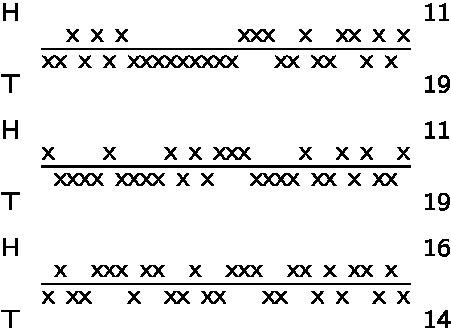
\includegraphics[width=0.8\linewidth]{fyz_fig077.pdf}
      \caption{Pozorované posloupnosti hlava znaků ve třech hrách po třiceti hodech 
              (\cite[s.~79]{Feynman01})}
      \label{fyz:fig077}
    \end{figure}
    Ve třech pokusech jsme ani jednou nedostali \num{15} hlav. Je to snad vinou mince? Nebo jsme se 
    zmýlili v úvaze vedoucí k závěru, že nejpravděpodobnější počet hlav v takové hře je \num{15}? 
    Abychom získali \num{100} experimentů, každý po \num{30} hodech, uskutečnili jsme dalších 
    \num{97} \uv{kol}. Výsledek experimentu ukazuje tab. \ref{fyz:fig079}\footnote{Po prvních třech 
    hrách jsme experiment ve skutečnosti provedli tak, že jsme silně zatřásli krabicí, v níž bylo 
    \num{30} mincí a pak jsme spočetli všechny hlavy.}.
    
    Prohlédneme-li si čísla v tab. \ref{fyz:fig079}, zjistíme, že většina výsledků je blízko čísla 
    \num{15} v tom smyslu, že se nacházejí mezi čísly \num{12} a \num{18}. K získání lepšího citu 
    pro chápání detailů těchto výsledků je vhodné zakreslit graf \emph{rozložení} výsledků. Určíme 
    počet her, v nichž jsme získali \(k\) hlav a znázorníme si je pro každé \(k\). Takový graf je 
    znázorněn na obr. \ref{fyz:fig078}. \num{15} hlav jsme získali ve \num{13} hrách. \num{14} 
    hlav jsme získali \num{13}-krát. \num{16} i \num{17} hlav jsme získali dokonce více než 
    \num{13}-krát.

    \begin{figure}[ht!]  %\ref{fyz:fig079}
      \centering
      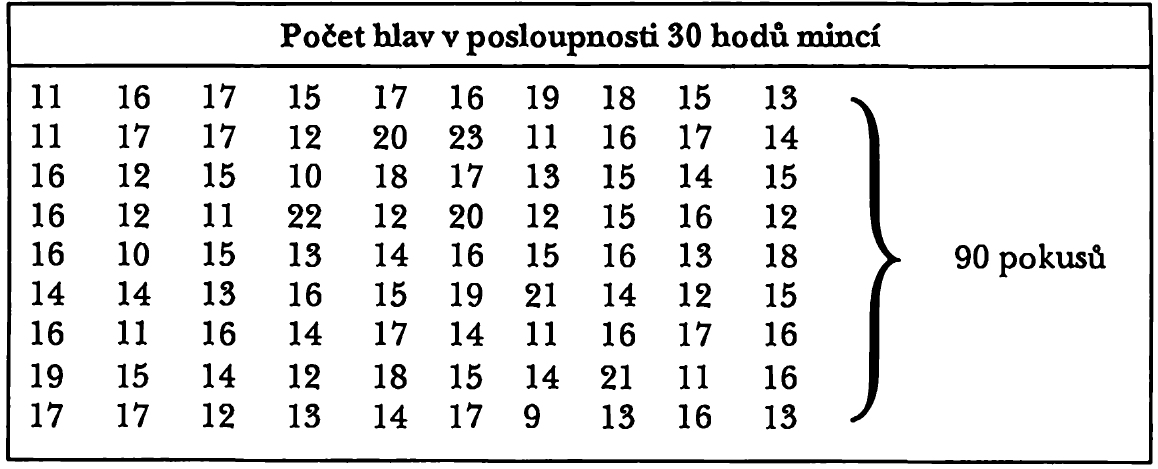
\includegraphics[width=1\linewidth]{fyz_fig079.png}
      \caption{Tabulka počtu hlav v posloupnosti \num{30} hodů mincí (\cite[s.~80]{Feynman01})}
      \label{fyz:fig079}
    \end{figure}
    Je možné z toho odvodit, že jde o jakousi zaujatost ve prospěch hlav? Nebyl náš „nejlepší 
    odhad“ dostatečně dobrý? Můžeme říci, že nejpravděpodobnější počet hlav pro jednu hru 
    sestávající z \num{30} hodů je \num{16}? Musíme být opatrní! Ve všech hrách se dohromady 
    uskutečnilo \num{3000} hodů. Hlav padlo celkem \num{1492}. Poměr počtu hlav k celkovému počtu 
    je tedy \num{0.497}, což je sice jen o málo, ale přece jen méně než polovina. Určitě tedy 
    nemůžeme předpokládat, že pravděpodobnost padnutí hlavy je větší než \num{0.5}! Skutečnost, že 
    v \emph{určité} sérii pozorování padne hlava nejčastěji \num{16}-krát, představuje 
    \emph{fluktuaci}. Jsme stále přesvědčeni, že \emph{nejpravděpodobnějším} počtem hlav je 
    \num{15}.
    
    Je možné položit otázku: Jaká pravděpodobnost, že hra s \num{30} hody dá \num{15}, \num{16} 
    nebo nějaký jiný počet hlav?“ Již jsme řekli, že při jednom hodu je pravděpodobnost pádu 
    \emph{jedné} hlavy \num{0.5} a i pravděpodobnost, že nepadne hlava, je \num{0.5}. Ve hře 
    sestávající ze dvou hodů máme \emph{čtyři} možné výsledky: \texttt{HH}, \texttt{HZ}, 
    \texttt{ZH}, \texttt{ZZ}. Protože každá z těchto posloupností je stejně pravděpodobná, můžeme 
    prohlásit, že
    \begin{enumerate}[noitemsep]
      \item pravděpodobnost padnutí dvou hlav je \num{1/4}, 
      \item pravděpodobnost padnutí jedné hlavy je \num{2/4}, 
      \item pravděpodobnost, že nepadne hlava je \num{1/4}. 
    \end{enumerate}
    Existují dva způsoby získávání jedné hlavy, ale jen jeden způsob získávání dvou hlav nebo žádné 
    hlavy.
    
    \begin{figure}[ht!]  %\ref{fyz:fig078}
      \centering
      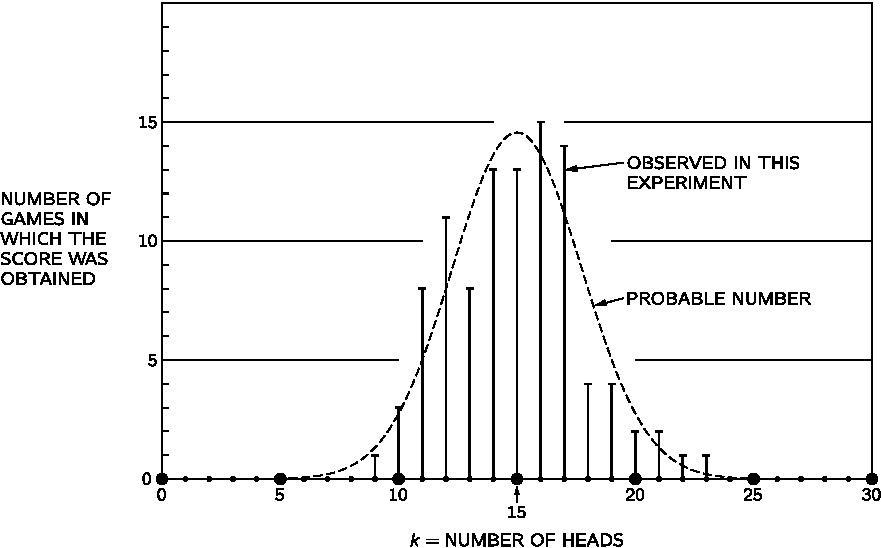
\includegraphics[width=1\linewidth]{fyz_fig078.pdf}
      \caption{Souhrn výsledků l00 her po 30pokusech. Vertikální čáry ukazuj počty her,v nichž 
              padlo \(k\) hlav. Přerušovaná čára ukazuje očekávaný počet her, v nichž padne \(k\) 
              hlav, získaný výpočtem pravděpodobnosti (\cite[s.~80]{Feynman01})}
      \label{fyz:fig078}
    \end{figure}
    
    Uvažujme nyní hru sestávající ze tří hodů. Pro třetí hod je stejně pravděpodobné, že padne 
    hlava nebo znak. Existuje jen jeden způsob získání tří hlav: v prvních dvou hodech 
    \emph{musely} padnout dvě hlavy a potom hlava i po třetím hodu. Existují však \emph{tři} 
    způsoby získání dvou hlav. Může padnout znak po padnutí dvou hlav (jeden způsob), nebo může 
    padnout hlava po padnutí jen jednoho znaku v prvních dvou hodech (dva způsoby). Tak pro možnosti
    \num{3}, \num{2}, \num{1}, \num{0} hlav existují \num{1}, \num{3}, \num{3}, \num{1} stejně 
    pravděpodobné způsoby představující celkově \num{8} různých posloupností. Příslušné 
    pravděpodobnosti jsou \num{1/8}, \num{3/8}, \num{3/8}, \num{1/8}.

    \begin{figure}[ht!]  %\ref{fyz:fig081}
      \centering
      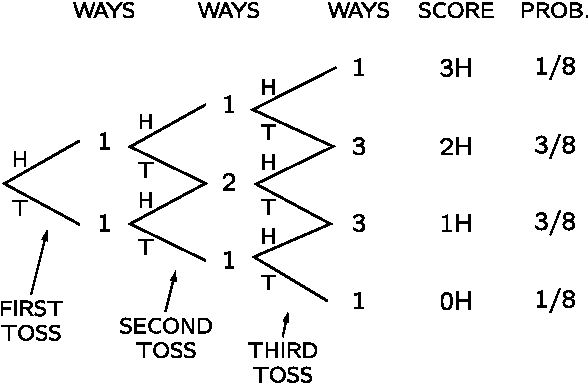
\includegraphics[width=1\linewidth]{fyz_fig081.pdf}
      \caption{Diagram znázorňující počet různých způsobů padnutí \num{0}, \num{1}, \num{2} nebo 
              \num{3} hlav ve hře sestávající ze tří hodů (\cite[s.~81]{Feynman01})}
      \label{fyz:fig081}
    \end{figure}
    
    To, co jsme řekli, je možno vyjádřit diagramem na obr. \ref{fyz:fig081}. Je jasné, že takové 
    diagramy lze sestrojit i pro hry s vyšším počtem hodů. Obr. \ref{fyz:fig080} znázorňuje takový 
    diagram pro hru se šesti hody. Počet způsobů odpovídajících libovolnému bodu diagramu je 
    vlastně počet různých cest (posloupností hlav a znaků), po nichž lze vyjít z počátečního bodu. 
    Počet úseků šikmo vzhůru udává počet vržených hlav. Soubor čísel, které se objevují v takovém 
    diagramu, je znám jako \textbf{Pascalův trojúhelník}. Čísla jsou známá i pod názvem 
    \emph{binomické koeficienty}, neboť se objevují i v rozvoji \((a + b)^n\). Označíme-li počet 
    hodů \(n\) a počet vržených hlav \(k\), pak se čísla vystupující v diagramu označují symbolem  
    \(\binom{n}{k}\). Bude vhodné připomenout, že binomické koeficienty 
    lze vypočítat ze vztahu
    \begin{equation}\label{fyz:eq074}
      \binom{n}{k} = \frac{n!}{k!(n-k)!}.
    \end{equation}
    kde \(n!\), nazývaný „n-faktoriál“, představuje součin \(n(n- 1)(n-2)\cdots (3)(2)(1)\).
    
    \begin{figure}[ht!]  %\ref{fyz:fig080}
      \centering
      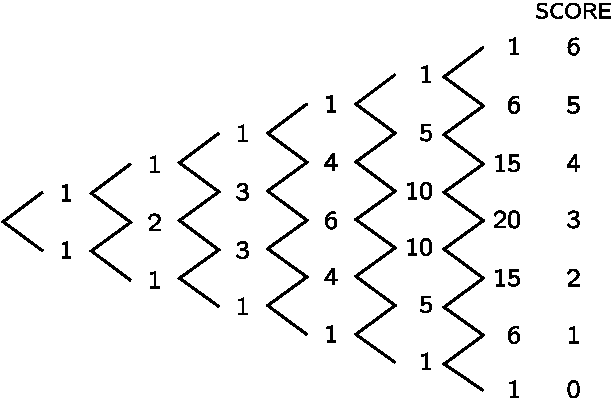
\includegraphics[width=1\linewidth]{fyz_fig080.pdf}
      \caption{Diagram jako na obr. \ref{fyz:fig081}, ale pro hru sestávající ze \num{6} hodů
               (\cite[s.~82]{Feynman01})}
      \label{fyz:fig080}
    \end{figure}
    
    Nyní již můžeme počítat pravděpodobnosti \(P(k, n)\) toho, že při \(n\) hodech padne hlava,
    pomocí definice (\ref{fyz:eq069}). Celkový počet možných posloupností je \(2^n\) (neboť každý
    hod připouští 2 výsledky) a počet způsobů získání \(k\) hlav je \(\binom{n}{k}\), přičemž
    všechny jsou stejně pravděpodobné. Proto máme
    \begin{equation}\label{fyz:eq075}
      P(k,n) = 
      \frac{\binom{n}{k}}{2^n}.
    \end{equation}
    
    Protože \(P(k, n)\) je podíl her, při nichž očekáváme, že padne \(k\) hlav, lze pak očekávat, 
    že při \num{100} hrách padne \(k\) hlav \(100\cdot P(k, n)\) krát. Přerušovaná čára na obr. 
    \ref{fyz:fig078} prochází body vypočítanými ze vztahu \(100\cdot P(k, 30)\). Vidíme, že padnutí 
    \num{15} hlav jsme \emph{očekávali ve} \num{14} nebo \num{15} hrách, zatímco tato událost byla 
    pozorována ve \num{13} hrách. Padnutí \num{16} hlav jsme \emph{očekávali ve} \num{13} nebo 
    \num{14} hrách, ale \num{16} hlav padlo v \num{16} hrách. Takové fluktuace jsou „součástí hry“.
    
    Použitou metodu je možné aplikovat i na tu nejobecnější situaci, v níž jsou jen dva možné 
    výsledky jednoho pozorování. Označme tyto dva výsledky \(V\) („výhra“) a \(P\) („prohra“). V 
    obecném případě pravděpodobnosti výsledku \(V\) nebo \(P\) u jedné události nemusí být stejné. 
    Označme \(p\) pravděpodobnost výhry \(V\). Potom \(q\), pravděpodobnost prohry, musí být nutně 
    \((1 - p)\). V souboru \(n\) pokusů je pravděpodobnost \(P(k, n)\) toho, že vyhrajeme 
    \(k\)-krát rovna
    \begin{equation}\label{fyz:eq076}
      \boxed{P(k,n) = \binom{n}{k}p^kq^{n-k}}\,.
    \end{equation}
    Tato pravděpodobnostní funkce se nazývá \textbf{Bernoulliho} nebo i \textbf{binomickou 
    pravděpodobností}.
    
  \section{Náhodná procházka}
    Existuje další zajímavý problém, v němž vystupuje myšlenka pravděpodobnosti. Je to problém 
    \emph{„náhodné procházky“}. Jako nejjednodušší verzi této úlohy si představme „hru“, v níž 
    „hráč“ startuje v bodě \(x = 0\) a při každém tahu má udělat krok \emph{buď} dopředu (směrem 
    \(k + x\)) nebo dozadu (směrem \(k - x\)). Volba se má uskutečnit náhodně, například pomocí 
    hodu mincí. Jak popíšeme výsledný pohyb? Ve své obecné formě se problém vztahuje na pohyb atomů 
    (nebo jiných částic) v plynech - jde o \textbf{Brownův pohyb} - a i na kombinaci chyb při 
    měřeních. Uvidíme, že problém náhodné procházky úzce souvisí s problémem házení mincí, o němž 
    jsme již hovořili.

    \begin{figure}[ht!]  %\ref{fyz:fig082}
      \centering
      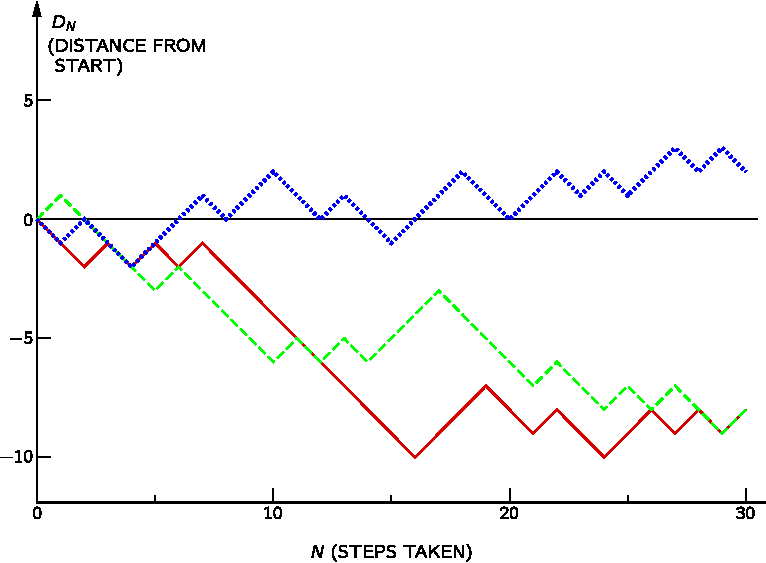
\includegraphics[width=1\linewidth]{fyz_fig082.pdf}
      \caption{Postup náhodné procházky. Horizontální souřadnice \(N\) představuje celkový počet 
               kroků: vertikální souřadnice \(D(N)\) představuje vzdálenost, do níž se chodec 
               dostal z počátečního bodu. (\cite[s.~83]{Feynman01})}
      \label{fyz:fig082}
    \end{figure}
    
    Nejprve si všimněme několika příkladů náhodné procházky. Postup chodce můžeme charakterizovat 
    čistou vzdáleností \(D_N\) ušlou v \(N\) krocích. Na obr. \ref{fyz:fig082} jsou vidět tři 
    příklady dráhy náhodného chodce. (Jako náhodné posloupnosti volby kroků jsme použili výsledky 
    házení mincí z obr. \ref{fyz:fig077}.)
    
    Co je možné říci o takovém pohybu? Především se můžeme ptát: Jak daleko se chodec v průměru 
    dostane?“ Musíme \emph{očekávat}, že jeho průměrný postup bude nulový, protože se stejně 
    pravděpodobně dostává dopředu nebo dozadu. Máme však takový pocit, že čím více \(N\) roste, tím 
    je pravděpodobnější, že chodec zabloudí dále od počátku. Proto se můžeme ptát, jaká je jeho 
    průměrná ušlá vzdálenost v \emph{absolutní hodnotě}, tj. jaký je průměr z \(\abs{D}\). Je však 
    výhodnější pracovat s jinou mírou „postupu“, se čtvercem vzdálenosti: \(D^2\) je kladné pro 
    kladný i záporný pohyb, a je proto vhodnou \emph{mírou} takového náhodného putování.
    
    Je možné dokázat, že očekávaná hodnota \(D_N^2\) je právě \(N\), tedy počet absolvovaných 
    kroků. „Očekávanou hodnotou“ rozumíme pravděpodobnou hodnotu (náš nejlepší odhad), kterou 
    můžeme považovat za \emph{očekávané} průměrné chování v mnoha opakovaných posloupnostech. 
    Takovou očekávanou hodnotu označujeme i \(\left\langle D_N^2\right\rangle\) a nazýváme ji i 
    \textbf{střední hodnotou čtverce vzdálenosti}. Po jednom kroku je \(D^2\) určitě rovno \(+1\), 
    máme tedy určitě \(\left\langle D_1^2\right\rangle = 1\). (Všechny vzdálenosti budou měřeny 
    tak, aby krok představoval jednotku. Jednotky vzdálenosti už nebudeme psát).

    Očekávanou hodnotu  \(\left\langle D_N^2\right\rangle\) pro \(N>1\) lze získat z \(D_{N-1}\). 
    Jestliže po \(N - 1\) krocích máme \(D_{N-1}\), pak po \(N\) krocích máme \(D_N = D_{N-1} + 1\) 
    nebo \(D_N = D_{N-1} - 1\). Pro druhé mocniny platí
    
    \begin{equation}\label{fyz:eq077}
      D_N^2 = 
        \begin{cases}
          D^2_{N-1} + 2D_{N-1} + 1 \\
          \quad\text{nebo}        \\
          D^2_{N-1} - 2D_{N-1} + 1
        \end{cases}
    \end{equation}
    Máme-li řadu nezávislých posloupností, očekáváme, že každá z těchto hodnot se objeví v polovině 
    případů, tedy naše průměrné očekávání je právě průměr ze dvou možných hodnot. Očekávaná hodnota 
    \(D_N\) je tedy \(D^2_{N-1} + 1\). Obecně můžeme očekávat pro \(D^2_{N-1}\) „očekávanou 
    hodnotu“  \(\left\langle D_{N-1}^2\right\rangle\) (podle definice !). Proto máme
    \begin{equation}\label{fyz:eq078}
      \left\langle D_N^2\right\rangle = \left\langle D_{N-1}^2\right\rangle + 1.
    \end{equation}
    Již jsme viděli, že \(\left\langle D_1^2\right\rangle = 1\) a proto musí být
    \begin{equation}\label{fyz:eq079}
      \left\langle D_N^2\right\rangle = N.
    \end{equation}
    Dostali jsme tedy velmi jednoduchý výsledek!
    
    Kdybychom při náhodné procházce chtěli „postup od začátku“ charakterizovat vzdáleností a ne 
    čtvercem vzdálenosti, museli bychom použít „střední kvadratickou vzdálenost“ \(D_{\text{stř}}\)
    \begin{equation}\label{fyz:eq080}
      D_{\text{stř}} = \sqrt{\left\langle D^2\right\rangle} = \sqrt{N}.
    \end{equation}
    
    Již jsme řekli, že náhodná procházka je z matematického hlediska velmi podobná hře házení 
    mincí, kterou jsme uvažovali na začátku kapitoly. Uvědomíme-li si, že směr každého kroku je v 
    souladu s padnutím hlavy nebo znaku ve hře s mincí, pak \(D\) je právě \(N_H - N_Z\), tedy 
    rozdíl počtu hlav a znaků. Protože je \(N_H + N_Z = N,\) kde \(N\) je celkový počet kroků (a 
    tedy i hodů), pak máme \(D = 2 N_H - N\). Již dříve jsme odvodili výraz pro očekávané rozdělení 
    \(N_H\) (nazývané i \(k\)) a dostali jsme výsledek (\ref{fyz:eq075}). Protože \(N\) je 
    konstanta, máme vlastně rozdělení odpovídající \(D\). (Protože pro každou hlavu navíc proti 
    \(N/2\) „chybí“ znak, máme faktor \(2\) mezi \(N_H\) a \(D\)). Grafy na obr. \ref{fyz:fig078} 
    představují rozdělení vzdáleností, jichž můžeme dosáhnout třiceti náhodnými kroky (kde \(k = 
    15\) znamená \(D = 0\), \(k= 16\), \(D = 2\) atd.).
    
    Odchylka \(N_H\) od očekávané hodnoty \(N/2\) je
    \begin{equation}\label{fyz:eq081}
      N_H - \frac{N}{2} = \frac{D}{2}
    \end{equation}
    a dále pro střední kvadratickou odchylku máme
    \begin{equation}\label{fyz:eq082}
      \left(N_H - \frac{N}{2}\right)_\text{stř} = \frac{1}{2}\sqrt{N}.
    \end{equation}
    
    V souladu s výsledky, které jsme získali pro \(D_{\text{stř}}\), očekáváme, že „typická“ 
    vzdálenost při třiceti krocích by měla být \(\sqrt{30} = \num{5.5}\), tedy typické \(k\) by 
    mělo být přibližně \(\num{5.5}/2 = \num{2.8}\) jednotek z \num{15}. Vidíme, že „šířka“ křivky 
    na obr. \ref{fyz:fig078} měřená od středu je přibližně \num{3} jednotky, což souhlasí s tímto 
    výsledkem.
    
    Dostali jsme se už tak daleko, že se můžeme zabývat otázkou, které jsme se dosud vyhýbali. Jak 
    můžeme rozhodnout, je-li mince „poctivá“ nebo „falešná“? Nyní můžeme na tuto otázku odpovědět 
    alespoň částečně. V případě poctivé mince očekáváme, že hlava se objeví v polovině případů, tj.
    \begin{equation}\label{fyz:eq083}
      \frac{\left\langle N_H\right\rangle}{N} = \num{0.5}.
    \end{equation}
    Očekáváme také, že skutečné \(N_H\) se bude lišit od \(N/2\) přibližně o \(\sqrt{N/2}\), nebo, 
    že podíl se bude lišit o
    \begin{equation}\label{fyz:eq084}
      \frac{1}{N}\cdot\frac{\sqrt{N}}{2} = \frac{1}{2\sqrt{N}}.
    \end{equation}
    Čím je \(N\) větší, tím blíže k jedné polovině bude podle našeho očekávání podíl \(N_H/N\).
    
    Na obr. \ref{fyz:fig083} je vynesen podíl \(N_H/N\) pro výše uvedenou hru s mincí. Z obrázku je 
    zřejmá snaha tohoto podílu dosáhnout hodnoty \num{0.5} při velkých \(N\). Naneštěstí pro žádnou 
    konkrétní hru nebo kombinaci her neexistuje \emph{záruka}, že pozorovaná odchylka bude alespoň 
    \emph{blízko očekávané odchylky}. Vždy existuje konečná možnost, že velká fluktuace - dlouhá 
    řada hlav nebo znaků způsobí libovolně velkou odchylku. Můžeme říci jen to, že v případě 
    odchylky, která se jen málo liší od hodnoty \(1/2\sqrt{N}\) (řekněme v rozsahu faktoru \num{2} 
    nebo \num{3}), nemáme důvod podezřívat minci z nepoctivosti. Je-li odchylka mnohem větší, může 
    vzniknout nedokazatelné podezření, že mince je upravena (nebo že hráč je příliš šikovný!).
    
    \begin{figure}[ht!]  %\ref{fyz:fig083}
      \centering
      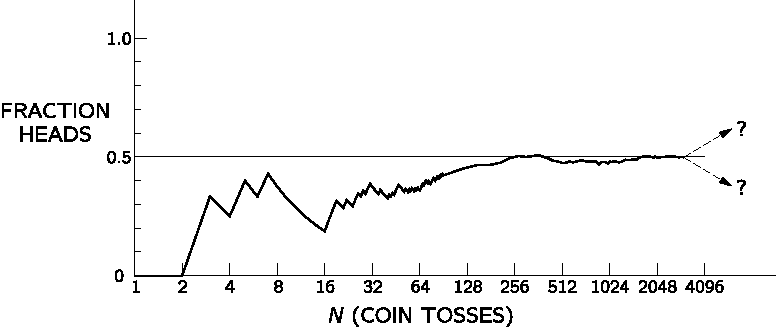
\includegraphics[width=1\linewidth]{fyz_fig083.pdf}
      \caption{Podíl hodů, v nichž padla hlava v určité posloupnosti \(N\) hodů mincí  
               (\cite[s.~85]{Feynman01})}
      \label{fyz:fig083}
    \end{figure}
    
    Nehovořili jsme ani o tom, co dělat v tom případě, kdy máme vážný důvod předpokládat, že 
    „mince“ nebo podobný jiný „náhodně“ se chovající předmět (například plochý kámen, který může 
    dopadnout jen na jednu nebo druhou stranu) \emph{budou mít} různé pravděpodobnosti, že padne 
    hlava nebo znak. Definovali jsme \(P(H) =\left\langle N_H\right\rangle/N\). Jak se dozvíme, co 
    je možné \emph{očekávat} pro \(N_H\). To nejlepší, co je možné v některých případech udělat, je 
    pozorovat počty hlav, které padnou při velkém počtu hodů. Z nedostatku lepší možnosti, musíme 
    položit \(\left\langle N_H\right\rangle = N_H\) (pozorované). (Co jiného je možné očekávat?) 
    Musíme si však uvědomit, že v takovém případě různé experimenty nebo různí pozorovatelé mohou 
    stanovit jinou hodnotu \(P(H)\). Je však možné \emph{očekávat}, že tyto hodnoty by se měly 
    lišit nejvýše odchylkou \(1/2\sqrt{N_H}\), je-li \(P(H)\) blízko \num{0.5}. Experimentální 
    fyzik říká, že „experimentálně určená“ pravděpodobnost má „chybu“ a píše
    \begin{equation}\label{fyz:eq085}
      P(H) = \frac{N_H}{N}\pm\frac{1}{2\sqrt{N}}.
    \end{equation}
    
    U takového výrazu se předpokládá, že \emph{existuje} „pravdivá“ nebo „správná“ pravděpodobnost, 
    kterou by bylo možné vypočítat, kdybychom toho dost věděli, a že pozorování mohou být zatížena 
    „chybou“ následkem fluktuace. Takovýto předpoklad však není možné logicky zdůvodnit. Je snad 
    lepší si uvědomit, že pojem pravděpodobnosti je svým způsobem subjektivní, že je vždy založen 
    na nejistých poznatcích a že jeho kvantitativní vyjádření podléhá změnám při získávání dalších 
    informací.
        
  \section{Rozložení pravděpodobnosti}
    Vraťme se opět k náhodné procházce a uvažujme o její obměně. Předpokládejme, že kromě náhodné 
    volby \emph{směru} (+ nebo -) každého kroku se mění i \emph{délka} kroku nějakým 
    nepředvídatelným způsobem, přičemž jedinou podmínkou je to, že v \emph{průměru} je délka kroku 
    jednotková. Takovýto případ lépe vystihuje něco takového, jako je tepelný pohyb molekul v 
    plynu. Je-li \(S\) délka kroku, pak \(S\) může dosáhnout jakékoli hodnoty, ale nejčastěji bude 
    \uv{blízko} \num{1}. Konkrétně budiž \(\left\langle S^2\right\rangle = 1\), nebo, což je totéž 
    \(S_{\text{stř}} = 1\). Při odvozování \(\left\langle D^2\right\rangle\) budeme postupovat jako 
    předtím, s tím rozdílem, že rovnice (\ref{fyz:eq078}) se nyní změní na
    \begin{equation}\label{fyz:eq086}
      \left\langle D_N^2\right\rangle 
        = \left\langle D_{N-1}^2\right\rangle + \left\langle s^2\right\rangle
        = \left\langle D_{N-1}^2\right\rangle + 1.
    \end{equation}
    Stejně jako předtím, i nyní dostaneme
    \begin{equation}\label{fyz:eq087}
      \left\langle D_N^2\right\rangle = N.
    \end{equation}
    Jaké bude nyní rozložení vzdáleností \(D\). Jaká je například pravděpodobnost toho, že \(D = 
    0\) po \num{30} krocích? Taková pravděpodobnost je nulová! Pravděpodobnost, že \(D\) bude 
    \emph{libovolná daná} hodnota, je nulová, neboť je zcela nepravděpodobné, že by součet všech 
    zpětných kroků (různých délek) byl přesně stejný jako součet kroků vpřed. Nemůžeme sestrojit 
    takový graf jako na obr. \ref{fyz:fig078}.
    
    Podobné znázornění jako na obr. \ref{fyz:fig078} je však možné, neptáme-li se na 
    pravděpodobnost \(D\) rovného přesně \num{0.1} nebo \num{2}, ale jestliže se zajímáme o 
    pravděpodobnost \(D\) \emph{v blízkosti} \num{0.1} nebo \num{2}. Definujme \(P(x, \Delta x)\) 
    jako pravděpodobnost toho, že \(D\) bude ležet v intervalu šířky \(\Delta x\) v okolí bodu 
    \(x\) (například od \(x\) po \(x + \Delta x\)). Očekáváme, že pro malé \(\Delta x\) je 
    pravděpodobnost toho, že \(D\) bude ležet v tomto intervalu, úměrná \(\Delta x\), tj. šířce 
    intervalu. Můžeme proto psát
    \begin{equation}\label{fyz:eq088}
      P(x,\Delta x) = p(x)\Delta x.
    \end{equation}
    Funkci \(p(x)\) nazýváme \textbf{hustotou pravděpodobnosti}.
    
    Tvar \(p(x)\) závisí na počtu kroků \(N\) i na rozdělení jednotlivých délek kroků. Nemůžeme to 
    zde dokazovat, ale pro velké \(N\) je hustota \(p(x)\) stejná pro všechna rozumná rozdělení 
    jednotlivých délek kroků a závisí jen na \(N\). Na obr. \ref{fyz:fig084} je znázorněno \(p(x)\) 
    pro tři hodnoty \(N\). Všimněte si, že pološířky těchto křivek (jejich rozšíření na úrovni 
    poloviny maximální výšky) jsou \(\sqrt{N})\) v souladu s našimi předcházejícími úvahami.
    
    Dále si můžeme všimnout, že hodnota \(p(x)\) v blízkosti nuly je nepřímo úměrná \(\sqrt{N}\). 
    Je tomu tak proto, že všechny křivky mají podobný tvar a plochy pod křivkami musí být stejné. 
    Protože \(p(x)\Delta x\) je pravděpodobnost nalezení \(D\) v \(\Delta x\) při malých hodnotách 
    \(\Delta x\), můžeme určit pravděpodobnost toho, že \(D\) se nachází někde uvnitř libovolného 
    intervalu ohraničeného body \(x_1\), \(x_2\) tak, že tento interval rozdělíme na malé části 
    \(\Delta x\) a vypočteme součet členů \(p(x)\Delta x\) pro každou takovou část.     
    Pravděpodobnost, že \(D\) se nachází někde mezi \(x_1\) a \(x_2\), což můžeme zapsat \(P(x_1 < 
    D < x_2)\), je rovna obsahu vyšrafované oblasti na obr. \ref{fyz:fig085}. Čím menší jsou 
    přírůstky \(\Delta x\), tím přesnější bude výsledek. Proto můžeme napsat, že
    \begin{equation}\label{fyz:eq089}
      P(x_1 < D < x_2) = \sum p(x)\Delta x = \int_{x_1}^{x_2}p(x)dx.
    \end{equation}
    Obsah plochy pod celou křivkou je pravděpodobnost, že \(D\) se někde nachází (tj. má nějakou 
    hodnotu mezi \(x=-\infty\) a  \(x= +\infty\)).

    \luagraphic[1]{fyz_fig084.pdf}{Hustota pravděpodobnosti dosažení vzdálenosti \(D\) od počátku
    při náhodné procházce sestávající z \(N\) kroků (\(D\) se měří v jednotkách střední kvadratické
    délky kroku) (\cite[s.~87]{Feynman01})}{fyz:fig084}
      
    Tato pravděpodobnost je rovna \(1\). Musí tedy být
    \begin{equation}\label{fyz:eq090}
      \int_{-\infty}^{\infty}p(x)dx = 1.
    \end{equation}
    
    Protože křivky na obr. \ref{fyz:fig084} se rozšiřují úměrně \(\sqrt{N}\), musí být jejich výška 
    úměrná \(1\sqrt{N}\), aby se zachoval celkový obsah plochy rovný \num{1}.

    \begin{figure}[ht!]  %\ref{fyz:fig084}
      \centering
      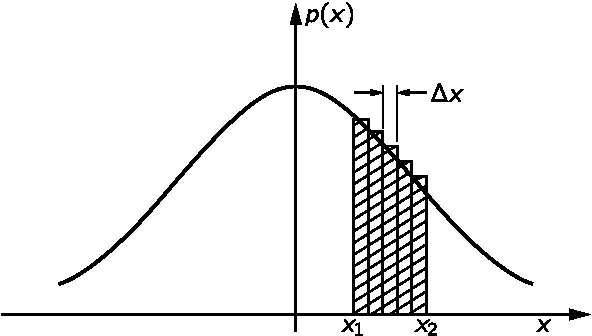
\includegraphics[width=1\linewidth]{fyz_fig085.pdf}
      \caption{Pravděpodobnost, že při náhodné procházce se ušlá vzdálenost \(D\) nachází mezi 
                body  \(x_1\) a \(x_2\), je dána obsahem plochy pod křivkou \(p(x)\) mezi \(x_1\) a 
                \(x_2\).
                \cite[s.~87]{Feynman01}}
       \label{fyz:fig085}
    \end{figure}
    
    S hustotou pravděpodobnosti, o níž jsme právě hovořili, se setkáváme nejčastěji. Je známá jako 
    \textbf{normální} nebo \textbf{Gaussova hustota pravděpodobnosti}. Její matematický zápis je
    \begin{equation}\label{fyz:eq091}
      p(x) = \frac{1}{\sigma\sqrt{2\pi}}e^{-\frac{x^2}{2\sigma^2}},	
    \end{equation}    
    přičemž veličina \(\sigma\) se nazývá \emph{standardní odchylkou}. V našem případě je \(\sigma 
    = \sqrt{N}\), nebo je-li střední kvadratická délka kroku různá od \num{1}, je 
    \(\sigma=\sqrt{N}S_\text{stř}\).
    
    Již jsme uvedli, že pohyb molekuly nebo každé jiné částice v plynu je podobný náhodné 
    procházce. Předpokládejme, že otevřeme láhev s organickou sloučeninou a necháme část její páry 
    uniknout do vzduchu. Existuje-li proudění vzduchu, tak že vzduch cirkuluje, budou unášeny i 
    uvedené páry. Jenže i v dokonale klidném vzduchu se budou páry postupně rozptylovat - 
    difundovat - dokud neproniknou do celé místnosti. Můžeme je registrovat podle jejich barvy nebo 
    zápachu. Jednotlivé molekuly organických par se šíří i v klidném vzduchu v důsledku 
    molekulárního pohybu způsobovaného srážkami s jinými molekulami. Známe-li délku „kroku“ a počet 
    kroků za sekundu, můžeme zjistit pravděpodobnost, v jaké vzdálenosti od svého původního místa 
    se ocitne po určitém čase jedna nebo několik molekul. Postupem času počet kroků roste a plyn se 
    rozplývá tak, jak je znázorněno křivkami na obr. \ref{fyz:fig084}. V jedné z dalších kapitol 
    určíme, jak závisí délka a frekvence kroků na teplotě a tlaku plynu.
    
    Již jsme hovořili o tom, že tak plynu je následkem srážek molekul se stěnami nádoby. Až později 
    přejdeme ke kvantitativnímu popisu tohoto jevu, musíme znát rychlost molekul narážejících na 
    stěnu, protože síla jejich nárazu závisí na rychlosti. Nemůžeme však hovořit o \emph{určité} 
    rychlosti molekul. Tento děj můžeme popsat jen pomocí pravděpodobností. Molekula může mít 
    jakoukoli rychlost, ale některé rychlosti jsou pravděpodobnější než jiné. Procesy probíhající v 
    plynu můžeme popsat pomocí pravděpodobnosti \(p(v)\Delta v\), že daná molekula má rychlost z 
    intervalu \(v, v+ \Delta v\). Hustota pravděpodobnosti \(p(v)\) je přitom funkcí rychlosti 
    \(v\). Později se dozvíte, jak Maxwell využitím zdravého rozumu a myšlenek teorie 
    pravděpodobnosti našel matematické vyjádření funkce \(p(v)\). Tvar\footnote{Maxwellův výraz je 
    \(p(v) = Cv^2e^{-av^2}\), kde \(a\) je konstanta související s teplotou a \(C\) je zvoleno tak, 
    aby celková pravděpodobnost byla rovna jedné.} funkce \(p(v)\) je znázorněn na obr. 
    \ref{fyz:fig086}. Rychlost může dosáhnout libovolné hodnoty, ale s největší pravděpodobností 
    bude blízká nejpravděpodobnější nebo očekávané hodnotě \(\langle v\rangle\)).
    
    \begin{figure}[ht!]  %\ref{fyz:fig086}
      \centering
      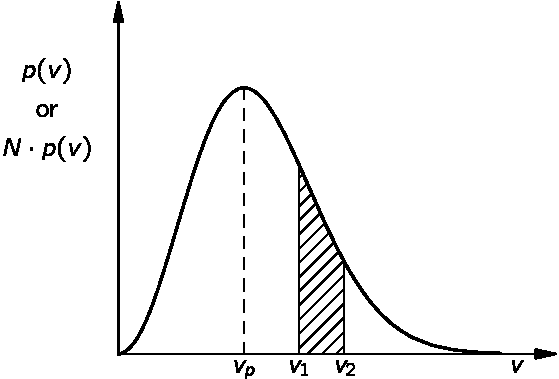
\includegraphics[width=1\linewidth]{fyz_fig086.pdf}
      \caption{Rozložení rychlosti molekul plynu  (\cite[s.~88]{Feynman01})}
      \label{fyz:fig086}
    \end{figure}
    
    O křivce znázorněné na obr, \ref{fyz:fig086} často uvažujeme trochu jinak. Máme-li molekuly 
    plynu uzavřené v typické nádobě (která má objem např. \SI{1}{\litre}), jde vlastně o velmi 
    velké množství \(N\) molekul (\(N\approx\num{e22}\)). Protože \(p(v)\Delta v\) je 
    pravděpodobnost toho, že \emph{jedna} molekula bude mít rychlost z intervalu \(\Delta v\), pak 
    podle naší definice pravděpodobnosti bude \emph{očekávaný} počet molekul \(\langle N\rangle\) s 
    rychlostmi z intervalu \(\Delta v\)
    \begin{equation}\label{fyz:eq092}
      \langle N\rangle = Np(v)\Delta v.
    \end{equation}
    Veličinu \(Np(v)\) proto nazýváme „\emph{rozdělením molekul podle rychlosti}“. Plocha pod 
    křivkou mezi dvěma hodnotami rychlosti \(v_1\) a \(v_2\), např. vyšrafovaná plocha na obr. 
    \ref{fyz:fig086}, představuje (v případě křivky \(Np(v)\)) očekávaný počet molekul s rychlostmi 
    mezi \(v_1\) a \(v_2\). Protože v případě plynu máme obvykle co činit s velkým počtem molekul, 
    předpokládáme malé odchylky od očekávaných hodnot (jako \(1/\sqrt{N}\)), a proto často 
    vynecháváme slovo „očekávaný“ a říkáme: „Počet molekul s rychlostmi mezi \(v_1\) a \(v_2\) 
    odpovídá obsahu příslušné plochy pod křivkou.“ Nesmíme však zapomenout, že takové výroky se 
    vždy týkají \emph{pravděpodobných} počtů.
    
  \section{Princip neurčitosti}
    Myšlenky pravděpodobnosti jsou jisté užitečné při popisu chování řádově \num{e22} molekul v 
    plynu, protože již samotný pokus o určení polohy nebo rychlosti každé molekuly by byl úžasně 
    nepraktický. Když se poprvé na takový problém aplikovala teorie pravděpodobnosti, chápalo se to 
    jako \emph{vhodný} způsob popisu tak složitých situací. Dnes jsme však toho názoru, že idea 
    pravděpodobnosti je při popisu atomových dějů \emph{nevyhnutelná}. Podle kvantové mechaniky, 
    matematické teorie částic, existuje vždy jistá nepřesnost při \emph{určení} poloh a rychlostí. 
    V nejlepším případě můžeme říci, že existuje jistá pravděpodobnost toho, že částice se bude 
    nacházet v blízkosti určitého bodu \(x\).
    
    Hustotu pravděpodobnosti \(p_1(x)\) udáme tak, že \(p_1(x)\Delta x\) představuje 
    pravděpodobnost výskytu částice mezi \(x\) a \(x+ \Delta x\). Je-li částice dostatečně dobře 
    lokalizovaná, např. v blízkosti \(x_1\), bude mít funkce \(p_1(x)\) průběh podobný grafu na 
    obr. \ref{fyz:fig087a}. Podobně musíme určit rychlost částice pomocí hustoty pravděpodobnosti 
    \(p_2(v)\), přičemž \(p_2(v)\Delta v\) je pravděpodobnost toho, že rychlost je v intervalu mezi 
    \(v\) a \(v+\Delta v\).
    
    \begin{figure}[ht!]  %\ref{fyz:fig087}
      \centering
      \subcaptionbox{\label{fyz:fig087a}}{\luafigure[0.70]{fyz_fig087a.pdf}}              \\
      \subcaptionbox{\label{fyz:fig087b}}{\luafigure[0.70]{fyz_fig087b.pdf}}
      \caption{Hustota pravděpodobnosti pozorování polohy a rychlosti částice  
               (\cite[s.~89]{Feynman01})}
      \label{fyz:fig087}
    \end{figure}
    
    Jeden ze základních výsledků kvantové mechaniky spočívá v tom, že funkce \(p_1(x)\) a 
    \(p_2(v)\) není možné vybrat nezávisle, zejména nemohou být obě dvě libovolně úzké. Označíme-li 
    charakteristickou „šířku“ křivky \(p_1(x)[\Delta x]\) a křivky \(p_2(v)\) zase \([\Delta v]\), 
    jak je ukázáno na obrázku, potom příroda vyžaduje, aby \emph{součin} těchto šířek nebyl menší 
    než číslo \(h/m\), kde \(m\) je hmotnost částice a \(h\) je základní fyzikální konstanta zvaná 
    \textbf{Planckova konstanta}. Tento základní vztah je možné zapsat ve tvaru
    \begin{equation}\label{fyz:eq093}
      [\Delta x][\Delta v]\geq\frac{h}{m}.
    \end{equation}
    Tato rovnice je matematickým vyjádřením \textbf{Heisenbergova principu neurčitosti}, o němž 
    jsme se již zmínili.
    
    Protože pravá strana rovnice (\ref{fyz:eq093}) je konstantní, pak, „přinutíme-li“ částici 
    zaujmout určité místo, skončí to tím, že velmi vzroste její rychlost. Nebo přinutíme-li částici 
    pohybovat se velmi pomalu, nebo velmi přesnou rychlostí, „rozplyne se“, takže nebudeme umět 
    říci, kde se přesně nachází. Částice se chovají velmi podivně!
    
    Princip neurčitosti vyjadřuje přirozenou nejasnost, která musí existovat při každém pokusu 
    popsat přírodu. Náš nejpřesnější popis přírody musí byt v řeči \emph{pravděpodobnosti}.Jsou 
    však lidé, kteří se neumějí smířit s takovýmto popisem přírody. Domnívají se, že kdybychom 
    věděli, co se s částicí  \emph{skutečně} děje, mohli bychom znát současně její přesnou rychlost 
    a polohu. Na začátku rozvoje kvantové mechaniky tento problém velmi znepokojoval Einsteina. 
    Často potřásal hlavou a říkal \uv{Vždyť bůh neháže kostkou, aby rozhodl, jak se má pohybovat 
    elektron!} Dlouho se trápil s tímto problémem a pravděpodobně se nikdy nesmířil se skutečnosti, 
    že je to ten nejlepší popis přírody, který dokážeme udělat. Několik málo fyziků se ještě stále 
    zabývá tímto problémem doufajíce, že svět je možné popsat nějak jinak a vyloučit neurčitost v 
    chování částic. Zatím však v tomto směru nikdo nebyl úspěšný. 
    
    Nevyhnutelná neurčitost při určování polohy částice nabývá významu tehdy, když chceme popsat 
    strukturu atomů. V atomu vodíku, jenž má jádro skládající se z jednoho protonu a mimo jádro má 
    jeden elektron, je neurčitost v poloze elektronu tak velká jako atom samotný! Proto nemůžeme 
    dost dobře hovořit o elektronu pohybujícím se po určité dráze kolem protonu. Nanejvýš můžeme 
    říci, že existuje určitá pravděpodobnost \(p(r)\Delta V\) pozorování elektronu v elementu 
    objemu \(\Delta V\) ve vzdálenosti \(r\) od protonu. Hustota pravděpodobnosti \(p(r)\) udává 
    kvantová mechanika. Pro neporušený vodíkový atom je \(p(r) = Ae^{-\frac{r^2}{a^2}}\), což 
    představuje funkci se zvonovitým grafem podobnou funkci na obr. \ref{fyz:fig085}. Číslo \(a\) 
    představuje \uv{charakteristický} poloměr, za nímž funkce rychle klesá. Protože je malá 
    pravděpodobnost výskytu elektronu ve větších vzdálenostech od jádra než \(a\), můžeme \(a\) 
    považovat za \uv{poloměr atomu}, což je asi \num{e-10} metru. 

    \begin{figure}[ht!]  %\ref{fyz:fig088}
      \centering
      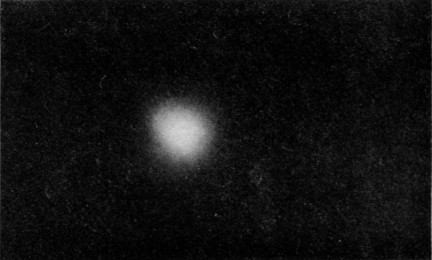
\includegraphics[width=0.8\linewidth]{fyz_fig088.jpg}
      \caption{Způsob znázornění atomu vodíku. Hustota (bělost) oblaku představuje hustotu 
               pravděpodobnosti výskytu elektronu. 
               (\cite[s.~90]{Feynman01})}
      \label{fyz:fig088}
    \end{figure}
    Představu o atomu vodíku můžeme získat, znázorníme-li si oblak, jehož hustota je úměrná hustotě 
    pravděpodobnosti výskytu elektronu. Příklad takového oblaku je na obr. \ref{fyz:fig088}. Naší 
    nejlepší \uv{představou} vodíkového atomu je tedy jádro obklopené \uv{elektronovým oblakem} (ve 
    skutečnosti však máme na mysli \uv{oblak pravděpdobnosti}). Elektron je někde tam, ale příroda 
    nám dovoluje poznat jen \emph{pravděpodobnost} jeho výskytu na určitém místě.
    
    Ve svém úsilí po co nejúplnějším poznání přírody dospěla moderní fyzika poznání, že jisté věci 
    není možné \uv{poznat} s jistotou. Mnohé z našich poznatků vždy zůstanou nejisté. Nanejvýš 
    můžeme znát jejich pravděpodobnosti. 
    
  \section{Příklady a cvičení}
  
%} %tikzset
%---------------------------------------------------------------------------------------------------
  % !TeX program = lualatex
% !TeX root = luaking.tex
% !TeX encoding = UTF-8
% !TeX spellcheck = cs_CZ
%---------------------------------------------------------------------------------------------------
\graphicspath{{../src/MAI/img/}}
% file mai1ch04b.tex
%---------------------------------------------------------------------------------------------------
\setchaptertoc
\chapter{Náhodné veličiny}\label{mai:IchapIVb}
  \epigraph{\emph{The true logic of this world is in the calculus of probabilities.}}{James Clerk 
    Maxwell}
  \section{Úvod}\label{mai:IchapIVsecIII}
    Hodnota některých veličin je určena jednoznačně a „jednou provždy“. Kdykoli budeme její hodnotu 
    zjišťovat, tehdy dostaneme totéž - takže ji ani opakovaně zjišťovat nemusíme. Příkladem může 
    být skoro prázdná peněženka, ve které jsou třeba tři koruny. Dokud nebudeme pracovat a do 
    peněženky něco nepřidáme, bude hodnota veličiny \(X\) (počet korun v peněžence) stále rovna 
    \num{3}. Nemá smysl se do peněženky vůbec dívat. Pokud budeme do peněženky přidávat každý den 
    dvě koruny, také budeme vědět, jak se veličina \(X\) mění, aniž bychom se do peněženky dívali. 
    Po \(n\) dnech bude hodnota \(X = 3 + 2n\). Většina veličin, se kterými se setkáváme, se však 
    takto nechová. Jejich hodnoty se totiž často řídí náhodnými vlivy, takže při každém
    měření veličiny \(X\), tj. zjišťování její hodnoty, můžeme získat odlišný výsledek než při 
    měřeních předchozích. Uveďme některé příklady náhodných veličin.
    
    \begin{itemize}
      \item \textbf{Příklad s novorozenci}: Nechť jé veličinou \(X\) počet chlapců ve stovce 
            novorozených dětí. Zkušenost říká, že tento počet je v průměru o něco větší než 
            \num{50}, avšak pro různé skupiny po stovce novorozených dětí bude počet chlapců 
            kolísat. V jedné skupině bude \num{52}, v jiné \num{54}, někde třeba \num{60}, nebo 
            také \num{45}.
      \item \textbf{Příklad s meteoroidy a meteority}: Pro astronomy může být důležitou veličinou 
            \(X\) počet meteoroidů, které za rok dopadnou do zemské atmosféry. Jinou veličinou, 
            třeba \(K\), může být roční počet meteoritů, tj. těch meteoroidů, které v atmosféře 
            neshořely zcela, ale jejich část dopadla na povrch Země. Také tyto hodnoty budou pro 
            každý roční interval poněkud odlišné, neboť i počet dopadnuvších meteoroidů a 
            meteoritů podléhá vlivům, které se nedají přesně předvídat.
      \item \textbf{ Příklad s tlakoměrem}: Bude-li lékař měřit pacientovi tlak několikrát po 
            sobě, určitě také naměří několik různých hodnot. Krevní tlak je citlivý na náhodné 
            vlivy, třeba i na vnitřní rozrušení pacienta vyplývající ze strachu z bílého pláště.
      \item \textbf{Opakovaná měření fyzikální veličiny}: Chceme-li změřit třeba odpor elektrického
            vodiče (drátu), jedná se o měření nepřímé. Nemůžeme odpor změřit přímo, třeba jako      
            to můžeme udělat pro délku. Většinou měříme napětí \(U\) na vodiči a proud \(I\), který 
            jím protéká. Odpor pak zjišťujeme jako podíl \(R = U/I\). Změříme-li napětí i proud 
            jednou, dostaneme konkrétní hodnotu \(R\). Budeme-li měření napětí a proudu provádět 
            opakovaně, budeme dostávat poněkud odlišné hodnoty \(U\) a \(I\), a tedy i odlišné 
            hodnoty \(R\). Sledované veličiny se chovají jako náhodné. Je to způsobeno řadou 
            náhodných vlivů jak na veličiny samotné, tak na jejich měření (nepřesnost odečítání 
            údajů na stupnicích, apod.).
    \end{itemize}
  
    Při každém fyzikálním (a vlastně i nefyzikálním) experimentu máme co do činění s náhodnými 
    veličinami. Při chemických analýzách je náhodnou veličinou třeba koncentrace dané látky
    v roztoku, při experimentech biologických třeba počet uhynuvších rostlin ve stovce sazenic, 
    počet pozorovaných prvoků v zorném poli mikroskopu, výskyt vzácných ptáků ve sledované 
    lokalitě, apod. V následujících odstavcích definujeme náhodné veličiny přesněji a naučíme se s 
    nimi zacházet. Uvidíme, že zjištění určité hodnoty náhodné veličiny je otázkou jisté 
    pravděpodobnosti. Také lépe objasníme, co znamená vyjádření „v průměru“, které jsme občas v 
    předchozím textu použili a intuitivně mu jistě rozuměli.
  
    \subsection{Jak dobrý je to střelec - diskrétní rozdělení}
      Mimořádně vhodnou ukázkou náhodné veličiny je příklad se sportovním střelcem, kterým jsme
      uvedli celou kapitolu o pravděpodobnostech.
  
      %--Ještě jednou střelba, tentokrát přesněji---------------------
      % !TeX spellcheck = cs_CZ
\begin{mdframed}[style=mdexam]
  \begin{example}\label{mai:exam064}
    \textbf{Ještě jednou střelba, tentokrát přesněji}\newline
    Názvem pochopitelně nemyslíme přesnější střelbu, ale přesnější komentář, který již bude založen
    na našich znalostech o pravděpodobnosti. Dejme tomu, že podmínky střelby jsou pevně dány a
    nemění se. Patří k nim zcela jistě typ zbraně, typ terče, vzdálenost stanoviště střelce od
    terče, základní povětrnostní podmínky. Výsledky jsou pak závislé na zručnosti střelce, avšak
    jsou ovlivněny náhodným i vlivy (foukne nenadálý vítr, střelec se lekne, zatřese se mu ruka,
    náhodně se mírně pozmění vzdálenost ústí hlavně od terče nebo její sklon, apod.). Počty
    dosažených bodů daného střelce při jednom výstřelu, nebo při sérii deseti výstřelů, atd., jsou
    tedy náhodnými veličinami. Pokusme se posoudit zručnost střelce přesněji. Označme jako náhodnou
    veličinu \(X\) počet bodů dosažených při jednom výstřelu. Nejprve určeme, jakých hodnot může
    nabývat. Všichni víme, jak vypadá běžný střelecký terč. Aby však naše počty nebyly příliš
    komplikované a zdlouhavé, uvažujme o terči mnohem jednodušším. Bude tvořen vnitřním černým
    kruhem s hodnotou \(3\) body, dále středním šedivým mezikružím s hodnotou \(2\) body a vnějším
    bílým mezikružím s hodnotou \(1\) bod. Střelba do terče mimo vnější kružnici nebo zcela mimo
    terč představuje bodovou hodnotu \(0\). Při jednom výstřelu tedy může střelec docílit v principu
    jakékoli z možných hodnot

    {\centering
      \captionsetup{type=figure}
      \luafigure[0.6]{mai_fig070.pdf}
      \captionof{figure}{Ilustrace k příkladu \ref{mai:exam064}}
      \label{mai:fig070}
    \par}
    \vspace{0.5em}
    \begin{equation*}
      X\in\{x_1, x_2, x_3,x_4\} = \{0,1,2,3\}.
    \end{equation*}
    Informace, jakých hodnot může náhodná veličina nabývat, je jistě nejen cenná, ale je pro
    jakékoli další úvahy nezbytná. Sama o sobě je však nepostačující. O střelcově zručnosti se na
    základě konstrukce terče nic nedovídáme. Kvalitativně jinou informaci získáme, víme-li, že
    možných hodnot zásahu dociluje střelec s následujícími pravděpodobnostmi:

    {\centering
      \begin{tabular}{c|rrrr}
        \(x_i\)    &      0     &      1     &      2     &      3       \\
        \hline
        \(p_i\)    & \num{0.03} & \num{0.28} & \num{0.52} & \num{0.17} 
      \end{tabular}
    \par}

    Můžeme tak třeba zjistit, kolika bodů střelec zhruba docílí s vysokou pravděpodobností při pěti
    výstřelech. Tento počet je
    \begin{gather*}
      5\cdot(\num{0.03}\cdot0 + \num{0.28}\cdot1 + \num{0.52}\cdot2 + \num{0.17}\cdot3) = 
      5\cdot\num{1.83} = \num{9.15} \simeq 9.
    \end{gather*}
    Pro každou pětici výstřelů může být počet dosažených bodů samozřejmě poněkud odlišný. Veličina
    \(Y\) představující počet dosažených bodů na pět výstřelů je rovněž veličinou náhodnou. Je nám
    však jasné, že hodnota dosažených bodů v každé pětici výstřelů je s vysokou pravděpodobností
    blízká číslu 9. Co to znamená „s vysokou pravděpodobností“? Dokážeme ji spočítat? Pokusme se o
    to. Především bychom museli určit, o kolik bodů se smí dosažený počet lišit od hodnoty 9,
    abychom jej ještě považovali za „blízký číslu 9“ . Tato volba závisí čistě na naší vůli a bude
    jí odpovídat i vypočtená pravděpodobnost. Dejme tomu, že zvolíme tento interval od 7 do 11 bodů
    včetně. Jev, jehož pravděpodobnost hledáme, je tedy
    \begin{itemize}
      \item \(A\) : Při pěti výstřelech získá střelec \num{7} nebo \num{8} nebo \num{9} nebo \num{10} 
            nebo \num{11} bodů.
      \item[] Jevy
      \item \(A_j\) : Střelec získá při pěti výstřelech \(j\) bodů.
    \end{itemize}
    jsou po dvou neslučitelné, pravděpodobnost jevu \(A\) tedy bude rovna součtu pravděpodobností
    \begin{equation*}
      p(A) = \sum_{j=7}^{11} p(A_j).
    \end{equation*}
   
    Pozor! Pravděpodobnosti \(p(Aj)\) jsou odlišné od pravděpodobností zadaných v první tabulce. Ta
    se totiž týká pěti výstřelů, zatímco tabulka \ref{mai:tab004} je pro jeden výstřel. Musíme tedy
    určit pravděpodobnosti \(p(A_j)\). K tomu je třeba zjistit všechny možnosti, jak docílit součtu
    bodů \(j\) pomocí pěti sčítanců nabývajících hodnot \num{0} až \num{3}. Soupis je v následující
    tabulce. Tabulka uvádí různé rozklady součtu na sčítance, počet případů, jak se tento rozklad
    realizuje (různé pořadí dosažených bodů při jednotlivých výstřelech) a pravděpodobnosti
    jednotlivých rozkladů zaokrouhlené na tři platná místa.

    Jak jsme spočítali pravděpodobnosti jednotlivých rozkladů? Dejme tomu, že počet bodů dosažených
    při pěti výstřelech je \(j\). Nechť \(j = j_1 + j_2 + j_3 + j_4 + j_5\) je rozklad hodnoty \(j\)
    na součet pěti sčítanců. Čísla \(j_1\) až \(j_5\) se pohybují od \num{0} do \num{3}, mohou být i
    shodná. Například jeden z možných rozkladů bodového součtu \(j = 9\) je \(9 = 3 + 2 + 2 + 1 +
    1\). Pravděpodobnost, že při pěti nezávislých výstřelech budou jednotlivé zásahy činit \(j_1\),
    \(j_2\), \(j_3\) , \(j_4\)a \(j_5\) bodů, je
    \begin{equation*}
      p_{j1}p_{j2}p_{j3}p_{j4}p_{j5}.
    \end{equation*}
    Pro případ zvoleného konkrétního rozkladu čísla \num{9} je to \(p_3p_2^2p_1^2\) - Zásahy s
    bodovým ziskem \(j_1\) až \(j_5\) mohou být realizovány v různých pořadích (například \(\num{3}
    + \num{2} + \num{2} + \num{1} + \num{1} = \num{2} + \num{3} + \num{2} + \num{1} + \num{1}
    =\ldots\), atd.). Označme počet všech takových pořadí \(n_{j_1\ldots j_5}\). (Pro \(j = \num{3}
    + \num{2} + \num{2} + \num{1} + \num{1}\) je \(n_{32211} = \binom{5}{2}\binom{3}{2} = 30\): Dvě
    z pěti pozic pro umístění dvou dvojek lze vybrat \(\binom{5}{2}\) způsoby, ze zbývajících tří
    pozic lze dvě pro umístění jedniček vybrat \(\binom{3}{2}\) způsoby a na trojku zbude poslední
    pozice.) Pravděpodobnost \(p_{j_1\ldots j_5}\) daného rozkladu čísla \(s\) pak je
    \begin{equation*}
      p_{j_1\ldots j_5} = n_{j_1\ldots j_5}p_{j_1}p_{j_2}p_{j_3}p_{j_4}p_{j_5}
    \end{equation*}

    {\centering
    \resizebox{1\textwidth}{!}{%
    \begin{tabular}{c|rrrr}
      součet \(j\)& sčítance   &    počet   & ppst rozkladu & \(p(A_j)\) \\ \hline
            7     & 3+3+1+0+0  & \num{30}   & \num{2.18e-4} & \num{0.102} \\
                  & 3+2+2+0+0  & \num{30}   & \num{1.24e-3} & \\
                  & 3+2+1+1+0  & \num{60}   & \num{1.25e-2} & \\
                  & 3+1+1+1+1  & \num{5}    & \num{5.22e-3} & \\
                  & 2+2+2+1+0  & \num{20}   & \num{2.36e-2} & \\
                  & 2+2+1+1+1  & \num{10}   & \num{5.94e-2} & \\ \hline
            8     & 3+3+2+0+0  & \num{30}   & \num{4.06e-4} & \num{0.185} \\
                  & 3+3+1+1+0  & \num{30}   & \num{2.04e-3} & \\
                  & 3+2+2+1+0  & \num{60}   & \num{2.32e-2} & \\
                  & 3+2+1+1+1  & \num{20}   & \num{3.88e-2} & \\
                  & 2+2+2+2+0  & \num{5}    & \num{1.10e-2} & \\
                  & 2+2+2+1+1  & \num{10}   & \num{1.10e-1} & \\ \hline
            9     & 3+3+3+0+0  & \num{10}   & \num{4.42e-5} & \num{0.238} \\
                  & 3+3+2+1+0  & \num{60}   & \num{7.57e-3} & \\
                  & 3+3+1+1+1  & \num{10}   & \num{6.34e-3} & \\
                  & 3+2+2+2+0  & \num{20}   & \num{1.43e-2} & \\
                  & 3+2+2+1+1  & \num{30}   & \num{1.08e-1} & \\
                  & 2+2+2+2+1  & \num{5}    & \num{1.02e-1} & \\ \hline
          10      & 3+3+3+1+0  & \num{20}   & \num{8.25e-4} & \num{0.215} \\
                  & 3+3+2+2+0  & \num{30}   & \num{7.03e-3} & \\
                  & 3+3+2+1+1  & \num{30}   & \num{3.53e-2} & \\
                  & 3+2+2+2+1  & \num{20}   & \num{1.34e-1} & \\
                  & 2+2+2+2+2  & \num{1}    & \num{3.80e-2} & \\ \hline
          11      & 3+3+3+2+0  & \num{20}   & \num{1.53e-3} & \num{0.133} \\
                  & 3+3+3+1+1  & \num{10}   & \num{3.85e-3} & \\
                  & 3+3+2+2+1  & \num{30}   & \num{6.56e-2} & \\
                  & 3+2+2+2+2  & \num{5}    & \num{6.21e-2} & \\ \hline
    \end{tabular}}
    \captionsetup{type=table} 
    \captionof{table}{Tabulka rozkladů pro daný součet bodů: ve sloupci \uv{počet} je uveden počet 
                      kombinací, které vedou ke stejnému nástřelu (sloupec \uv{součet}) a s daným
                      bodovým ohodnocením (sloupec \uv{sčítanec})}
    \label{mai:tab004}
    \par}
    \vspace{\baselineskip}

    Pro rozklad \(\num{9} = \num{3} + \num{2} + \num{2} + \num{1} + \num{1}\) je (výsledek viz také
    v tabulce)
    \begin{equation*}
      p_{32211} =30\cdot p_3p_2^2p_1^2 = \num{30}\cdot\num{0.17}\cdot\num{0.52}^2\cdot\num{0,282} 
                \simeq \num{0.108}.
    \end{equation*}
    Pravděpodobnost \(p(A_j)\) je součtem pravděpodobností jednotlivých rozkladů čísla \(j\).
    Konečně pravděpodobnost, že střelec dosáhne bodového výsledku \(y \in [7, 11]\), je rovna součtu
    pravděpodobností \(p(A_j)\) pro \(j = 7, 8, 9, 10, 11\). Tato hodnota je \num{0.873}, tedy
    opravdu poměrně vysoká, jak jsme očekávali. Také bychom mohli říci, že střelec dosahuje při
    každé pětici výstřelů „v průměru“ \num{9} bodů, a tedy při jednom výstřelu „v průměru“ \num{1.8}
    bodů. Pokud bychom „průměrnou hodnotu“ jednoho výstřelu počítali i pro jiný počet výstřelů než
    pro pět, budeme dostávat čísla, která budou hodnotě \num{1.8} velmi blízká.
  \end{example}
\end{mdframed}
      %---------------------------------------------------------------
    
    Položme si ještě otázku, jak můžeme zjistit pravděpodobnosti, se kterými střelec dosáhne při
    jednom výstřelu daného počtu bodů. Prakticky to lze provést jedině tak, že střelec mnohokrát
    vystřelí na terč a jeho zásahy budou při tom zaznamenávány. Dejme tomu, že vystřelil \(n\)-krát 
    a že počet výstřelů, při nichž byl bodový zisk \(j\) bodů ( \(j = 0, 1, 2, 3\)), byl \(n_j\). 
    Pak pro pravděpodobnost bodového zisku \(j\) bodů při jednom výstřelu je \(p_j = n_j/n\). 
    Kdybychom provedli skutečný experiment se střelcem a počítali pravděpodobnosti \(p_j\) znovu a 
    znovu po každém dalším výstřelu, viděli bychom, že pro malé hodnoty \(n\) nejprve kolísají a 
    pro rostoucí \(n\) se začínají ustalovat a již kolísají velmi málo. Tímto postupem bychom je 
    mohli určit tak, aby byly pro náš účel rozumně přesné - třeba s přesností na dvě platná místa. 
    Rozumnou přesností je zde myšlena skutečnost, že nemá smysl chtít zjišťovat pravděpodobnost 
    třeba na šest platných míst. Vzhledem k principiální přítomnosti náhodných vlivů se kolísání 
    pravděpodobností nikdy nezbavíme, takže platná místa na pozicích, kde se kolísání trvale 
    projevuje již bez ohledu na zvyšující se \(n\), nemají smysl.
    
    V příkladu \ref{mai:exam064} jsme se již velmi těsně přiblížili důležitým charakteristikám, 
    které určují náhodnou veličinu a jsou přitom matematicky korektně definovány. Viděli jsme, že 
    známe-li jen hodnoty, kterých může náhodná veličina nabývat, nemůžeme o ní říci již nic 
    dalšího. Známe-li však ještě pravděpodobnosti, se kterými jednotlivých hodnot nabývá, můžeme o 
    ní získat již velmi mnoho informací.

    \begin{mdframed}[style=highlight]
      \textbf{Náhodnou veličinou s diskrétním rozdělením} nazýváme takovou veličinu \(X\), která
      může nabývat konečně mnoha různých hodnot \((x_1, x_2, \ldots, x_k)\) s pravděpodobnostní
      \((p_1, p_2, \ldots, p_k)\) popřípadě spočetně mnoha hodnot \((x_1, x_2, \ldots)\) s 
      pravděpodobnostmi \((p_1, p_2, \ldots)\).
    \end{mdframed}

    Jevy \(A_j\) \uv{veličina \(X\) nabývá hodnoty \(x_j\)}, jsou po dvou neslučitelné. Platí
    \begin{equation*}
      \sum_{j=1}^{k}p_j = 1, \qquad\text{resp.}\qquad \sum_{j=1}^{k=\infty}p_j = 1
    \end{equation*}
    Pokud jde o druhý z obou případů, nebudeme se jím prozatím zabývat. Soubor všech dvojic
    \begin{equation*}
      \left\lbrace(x_j, p_j)\right\rbrace,\qquad j = 1, 2, \ldots, k,
    \end{equation*}
    se nazývá \textbf{rozdělení} náhodné veličiny \(X\). Můžeme je znázornit i graficky.

    %--Bernoulliovo (binomické) rozdělení---------------------------
    % !TeX spellcheck = cs_CZ
\begin{mdframed}[style=mdexam]
  \begin{example}\label{mai:exam065}
    \textbf{Bernoulliovo (binomické) rozdělení}\newline
    Představme si opět Bernoulliův pokus o \(n\) opakováních a pravděpodobností zdaru při jednom
    opakování rovnou \(p\) (kapitola \ref{mai:IchapIVsecIIssecIV}). Náhodnou veličinu \(X\)
    definujme jako počet zdarů při tomto pokusu. Tato veličina nabývá všech celočíselných hodnot
    \(x_j = j, 0 \leq j \leq n\), přitom hodnoty \(j\) nabývá s pravděpodobností určenou vztahem
    (\ref{mai:eq055}), v němž za \(x\) dosadíme \(j\). 
    
    {\centering
      \captionsetup{type=figure}
      \luafigure[1]{mai_fig044.pdf}
      \captionof{figure}{Bernoulliovo rozdělení
      \cite[s.~229]{Musilova2009MA1}
      \label{mai:fig044}}
    \par}
    
    Získané rozdělení je tedy
    \begin{equation*}
      \lbrace j,p_j\rbrace, \quad\text{kde}\quad p_j = \binom{n}{j}p^j(1 - p)^{n-j}.
    \end{equation*}
    Graf Bernoulliova rozdělení, které je často nazýváno také binomickým, je na obrázku 
    \ref{mai:fig044} pro \(n = 15\) a \(p = 1/2\) (červený asterisk).
    
    Z grafu je názorně vidět, co to znamená, že některé hodnoty veličiny \(X\) jsou více a jiné méně 
    pravděpodobné. Hodnota \(x_i\), veličiny \(X\), které odpovídá největší pravděpodobnost \(p_i\), 
    se nazývá nejpravděpodobnější hodnota. V případě Bernoulliova rozdělení na obrázku 
    \ref{mai:fig044} jsou takové hodnoty dvě, konkrétně \(x_7 = 7\) a \(x_8 = 8\).
    
      \begin{lstlisting}[style=luaCPPStyle, caption={PPST001.m}]
        citatel= factorial(n);
        jmenovatel= factorial(n-j).*factorial(j);
        binom = citatel./jmenovatel;
        f = binom.*p.^j.*(1-p).^(n-j);
      \end{lstlisting}
  \end{example}
\end{mdframed}
    %---------------------------------------------------------------
    
    Nyní definujeme další charakteristiky náhodné veličiny. Těmi základními jsou, kromě již 
    definované \emph{nejpravděpodobnější hodnoty}, ještě \textbf{střední hodnota}, \textbf{rozptyl} 
    (popřípadě jeho odmocnina, zvaná \textbf{střední kvadratická} nebo \textbf{směrodatná 
    odchylka}), \textbf{medián}, popřípadě \textbf{P-kvantil}. Pojem střední hodnoty jsme již v 
    podstatě vybudovali v příkladu se střelcem. Nyní postup zobecníme. Předpokládejme, že při 
    velkém počtu \(n\) měření náhodné veličiny \(X\) naměříme různé hodnoty \((x_1, x_2, \ldots, 
    x_k)\) tak, že hodnota \(x_1\) byla naměřena \(n_1\)-krát, hodnota \(x_2\) \(n_2\)-krát, atd., 
    až hodnota \(x_k\) \(n_k\)-krát. Je zřejmé, že součet četností \(n_1\), \(n_2\), až \(n_k\) 
    jednotlivých hodnot musí být roven celkovému počtu měření \(n\) a že podíly
    \begin{equation*}
      p_1 = \dfrac{n_1}{n}, \qquad p_2 = \dfrac{n_2}{n}, \qquad \ldots, \qquad p_k = \dfrac{n_k}{n},
    \end{equation*}
    představují pravděpodobnosti jednotlivých hodnot veličiny \(X\). Tím je zadáno její rozdělení,
    které ji plně charakterizuje. Položme si však otázku, zda by se veličina \(X\) přece jen nedala
    charakterizovat jedinou hodnotou, která by všechny různě pravděpodobné hodnoty v jistém
    smyslu „zastupovala“. Kdybychom třeba takto měřili délku stolu, jistě bychom na otázku „Kolik
    měří stůl?“ neodpovídali tím, že bychom tazateli předložili získané rozdělení, i když by taková
    odpověď byla nejvýstižnější. Určitě bychom uvedli jedinou hodnotu. Ale jakou? I laika napadne,
    že by takovou reprezentativní hodnotou mohl být aritmetický průměr naměřených hodnot \(x_1\) až
    \(x_k\). Bylo by ale správné vzít jen prostý aritmetický průměr těchto různých hodnot a nebrat 
    ohled na skutečnost, že některé byly naměřeny s větší a jiné s menší četností? Nikoliv. 
    Reprezentativní hodnota veličiny \(X\) nemá zastupovat jen naměřené hodnoty, ale celé 
    rozdělení. Určitá hodnota \(x_j\) bude mít tím větší vliv na reprezentativní hodnotu, s čím 
    větší četností byla naměřena. Protože byla naměřena \(n_j\)-krát, musíme ji také tolikrát do 
    aritmetického průměru započíst.Získáváme tak \textbf{vážený aritmetický průměr} naměřených 
    hodnot, neboli \emph{střední hodnotu}
    
    \begin{mdframed}[style=highlight]
      \begin{align}\label{mai:eq059}
        \left\langle x \right\rangle 
          &= \dfrac{n_1x_1 + n_2x_2 + \cdots + n_kx_k}{n}  \nonumber \\
          &= p_1x_1 + p_2x_2 + \cdots + p_kx_k             \nonumber \\
          &= \sum_{j=1}^{k}p_jx_j.
      \end{align}
    \end{mdframed}
    Součet všech pravděpodobností \(p_1 + p_2 + \cdots + p_k\) je pochopitelně \textbf{roven jedné}.

    %--Střední hodnota Bernoulliova rozdělení-----------------------
    % !TeX spellcheck = cs_CZ
\begin{mdframed}[style=mdexam]
  \begin{example}\label{mai:exam066}
    \textbf{Bernoulliovo (binomické) rozdělení}\newline
    Pro střední hodnotu Bernoulliova rozdělení platí
    \begin{equation*}
      \langle j \rangle = \sum_{j=0}^{n}j\cdot p_j
        = \sum_{j=1}^{n}j\begin{pmatrix} n \\ j \end{pmatrix}p^j(1-p)^{n-j} = np.
    \end{equation*}
    
    Tento vztah lze dokázat matematickou indukcí vzhledem k proměnné \(n\). Na tomto místě nebudeme
    důkaz provádět pro jeho poměrnou zdlouhavost. Každý jej však může zvládnout. Vzpomeňme si v tuto
    chvíli na náš chybný intuitivní odhad v kapitole \ref{mai:IchapIVsecIIssecIV}, v níž jsme
    poprvé hovořili o Bernoulliově pokusu v souvislosti s hody mincí. Chybně jsme tam odhadli
    pravděpodobnost, že při \(n\) opakováních pokusu nastane v polovině z nich zdar. Tato chyba
    vznikla v důsledku naší zkušenosti, že když budeme mincí vícekrát házet, padne hlava (zdar)
    skutečně zhruba v polovině případů. Vidíme nyní, že \(n/2\) reprezentuje střední hodnotu náhodné
    veličiny \(X =\) \textbf{počet zdarů při \(n\) hodech mincí}. A to naší zkušenosti již odpovídá.
  \end{example}
\end{mdframed}
    %---------------------------------------------------------------
    
    Posuďme nyní situaci, kdy náhodná veličina \(Y\) je funkcí náhodné veličiny \(X, Y = f(X)\).
    V takovém případě má rozdělení veličiny \(Y\) tvar
    \begin{equation*}
      \left\lbrace (f(x_j), p_j)\right\rbrace, \qquad j = 1, 2, \ldots, k.
    \end{equation*}
    Pravděpodobnost hodnoty \(f(x_j)\) je stejná jako pravděpodobnost hodnoty \(x_j\). Pro výpočet
    střední hodnoty veličiny \(Y\) pak platí
    \begin{equation}\label{mai:eq060}
      \left\langle y \right\rangle = \sum_{j=1}^{k}f(x_j)p_j.
    \end{equation}
    (V obecnější situaci může být náhodná veličina \(Y\) funkcí několika náhodných veličin \(X_1\), 
    \(X_2\), až \(X_s\)).
    
    Může vzniknout oprávněná otázka, zda při výpočtu \(\left\langle y \right\rangle\), popřípadě 
    dalších charakteristik veličiny \(Y\), nevznikne nějaký problém, nebude-li funkce \(f(X)\) 
    prostá. V takovém případě by totiž některé hodnoty veličiny \(Y\) splynuly i pro různá \(x_j\). 
    Například pro \(Y = f(X) = X^2\) by pro hodnoty \(x_r\) a \(x_s\) vázané vztahem \(x_r = -x_s\) 
    (pokud by veličina \(X\) směla takových hodnot nabývat) platilo \(y_{rs} = y_r = y_s\). 
    Pravděpodobnost této společné hodnoty by pak přece byla \((p_r + p_s)\). Tato úvaha je 
    samozřejmě správná, avšak ve výpočtu střední hodnoty veličiny Y
    podle vztahu (\ref{mai:eq060}) je již obsažena. Do součtu totiž vstupují sčítance \(y_rp_r\) i 
    \(y_sp_s\), jejichž součet je při rovnosti \(y_r = y_s\) roven \(y_{rs}(p_r +p_s)\) Společná 
    hodnota \(y_{rs}\) je tedy započtena se správnou vahou.
    
    Uvažujme nyní o tom, jak „směrodatná“, tj. do jaké míry opravdu „reprezentativní“, je
    střední hodnota náhodné veličiny. Intuitivně cítíme, že střední hodnota bude reprezentovat
    rozdělení náhodné veličiny tím lépe, čím méně se od ní budou jednotlivé hodnoty odchylovat na 
    obě strany. Význam slova „odchylovat“ musíme ovšem nějak kvantitativně zachytit.
    \emph{Odchylkou} hodnoty \(x_j\) veličiny \(X\) od střední hodnoty \(\left\langle x 
    \right\rangle\) budeme celkem přirozeně rozumět rozdíl \((x_j - \langle x\rangle)\). Vzniká tak 
    náhodná veličina \(\Sigma = X - \langle x \rangle\) s rozdělením \(\{(x_j - \langle x\rangle, 
    p_j)\}\), \(j = 1, 2, \ldots, k\) . Bude tou správnou charakteristikou odchýlení hodnot 
    veličiny \(X\) od střední hodnoty střední hodnota \(\langle\sigma\rangle\)? Vypočtěme ji 
    (odhadněte předem, co asi tak vyjde):
    \begin{align*}
      \langle\sigma\rangle 
          &= \sum_{j=1}^{k}(x_j - \langle x\rangle)p_j
           = \sum_{j=1}^{k}x_jp_j - \langle x\rangle\sum_{j=1}^{k}p_j   \\
          &= \langle x\rangle - \langle x\rangle = 0.
    \end{align*}
    Čekali jste to? Nepochybně ano. Veličina \(X - \langle x\rangle\) nedává tedy žádný obraz o 
    tom, jak jsou hodnoty \(x_j\) „rozptýleny“ okolo střední hodnoty \(\langle x\rangle\). Kladné 
    odchylky jsou to tiž kompenzovány těmi zápornými. Aby k takové kompenzaci nedošlo, stačí vzít 
    v úvahu absolutní hodnotu veličiny \(\Sigma\), popřípadě její kvadrát. Vezměme v úvahu druhý z 
    obou námětů a vypočtěme \(\langle \sigma^2\rangle\), takzvaný \textbf{rozptyl veličiny} \(X\):
    \begin{align}\label{mai:eq061}
       D(X) &= \langle \sigma\rangle = \sum_{j=1}^{k}(x_j - \langle x\rangle)^2p_j    \nonumber \\
            &= \sum_{j=1}^{k}x_j^2p_j - 2\langle x\rangle\sum_{j=1}^{k}x_jp_j 
              + \langle x\rangle^2\sum_{j=1}^{k}p_j                                   \nonumber \\
            &= \langle x^2\rangle - 2\langle x\rangle^2 + \langle x\rangle^2          \nonumber \\
            &= \langle x^2\rangle - \langle x\rangle^2.
    \end{align}
    hodnota
    \begin{mdframed}[style=highlight]
      \begin{equation}\label{mai:eq062}
        \sigma(x) = \sqrt{\langle \sigma^2\rangle} = \sqrt{\langle x^2\rangle - \langle x\rangle^2}
      \end{equation}
    \end{mdframed}
    se nazývá \textbf{směrodatná odchylka} (v některých terminologiích též \emph{střední 
    kvadratická odchylka}) veličiny \(X\). Podíl \(\sigma(x)/ \langle x\rangle\) se nazývá 
    \textbf{relativní směrodatná odchylka} (v některé terminologii též \emph{variační koeficient}).

    \begin{mdframed}[style=highlight]
      Důležitým pojmem je \textbf{distribuční funkce}. Je to funkce \(F\) jedné reálné proměnné 
      \(x\) definovaná ve vztahu k náhodné veličině \(X\) takto: Předpokládejme, že hodnoty \(x_1\)
      až \(x_k\), jichž může náhodná veličina \(X\) nabývat, jsou seřazeny vzestupně, tj. \(x_1 <
      < x_2 < \ldots < x_k\). Pak
      \begin{equation}\label{mai:eq063}
        F: \realset\ni x\longleftrightarrow 
        F(x) = \sum_{\mathclap{\substack{j=1\\ x_s \leq x \leq x_{s+1}}}}^{s}p_j
      \end{equation}
    \end{mdframed}

    Přestože je veličina \(X\) diskrétní, je distribuční funkce funkcí spojité proměnné. Její 
    funkční hodnoty se však mění skokem. Vidíme to z následující tabulky a z grafu na obrázku 
    \ref{mai:fig045}, v němž je distribuční funkce znázorněna pro případ střelby (příklad 
    \ref{mai:exam064})

    \begin{table}[ht!]
      \centering
      \begin{tabular}{c|c}
        \textbf{interval}                 &  \textbf{distribuční funkce}             \\ \hline
            \(-\infty, x_1\)              &    \(F(x) = 0\)                         \\
            \(\left[x_1, x_2\right)\)     &    \(F(x) = p_1\)                       \\
            \(\left[x_2, x_3\right)\)     &    \(F(x) = p_1 + p_2\)                 \\
                    \(\ldots\)            &       \(\ldots\)                         \\
            \(\left[x_j, x_{j+1}\right)\) &    \(F(x) = p_1 + p_2 + \cdots + p_j\)  \\
                   \(\ldots\)             &       \(\ldots\)                         \\
            \(\left[x_k, \infty\right)\)  &    \(F(x) = p_1 + \cdots + p_k =1\)     \\ \hline
            \end{tabular}
      % \caption{ }
    \end{table}

    \luagraphic[1]{mai_fig045.pdf}{Distribuční funkce k příkladu \ref{mai:exam064}. 
    \cite[s.~233]{Musilova2009MA1}}{mai:fig045}

    Zadáním distribuční funkce je naopak jednoznačně určeno rozdělení veličiny \(X\). Pro jednotlivé
    pravděpodobnosti totiž platí
    \begin{equation*}
      p_j = F(x_j) - F(x_{j-1})\;\text{pro}\; 2\leq j \leq k, \; p_1 = F(x_1).
    \end{equation*}
    
    Hledejme nyní hodnotu \(\overline{x}_P\) definovanou tak, že pravděpodobnost, že při náhodném 
    opakování pokusu nabude veličina \(X\) kterékoli z přípustných hodnot \(x_j \leq 
    \overline{x}_p\), je rovna \(P\). Znamená to, že pro \(x = \overline{x}_P\) má distribuční 
    funkce nabýt předepsané hodnoty \(P\). Abychom \(\overline{x}_P\), takzvaný 
    \(P\)\textbf{-kvantil}, určili, řešíme rovnici
    \begin{equation}\label{mai:eq064}
      \sum_{j=1}^{s}p_j = P
    \end{equation}
    vzhledem k neznámému počtu sčítanců \(s\). V případě veličiny s diskrétním rozdělením se ovšem
    může stát, že pro nevhodně zvolenou hodnotu \(P\) nebude mít rovnice řešení. To proto, že 
    veličina \(X\) může nabývat jen hodnot, které lze očíslovat přirozenými čísly, takže při každé 
    změně horní meze sumy \(s\) o jedničku se suma mění skokem. Vidíme to jak v předcházející 
    tabulce, tak v grafu na obrázku \ref{mai:fig045}. Pro \(P = \num{0.5}\) se \(P\)-kvantil 
    \(\overline{x}_p\), pokud je vůbec definován, nazývá \textbf{medián}. Značí se pouze 
    \(\overline{x}\).

    %--Ještě střelba------------------------------------------------
    % !TeX spellcheck = cs_CZ
\begin{mdframed}[style=mdexam]
  \begin{example}\label{mai:exam067}
    \textbf{Ještě střelba}\newline
    Problém s definici \(P\)-kvantilu u veličiny s diskrétním rozdělením snadno vidíme na příkladu
    střelby (příklad \ref{mai:exam064}). Pro \(s\) postupně 1, 2, 3, 4 nabývá součet na levé straně
    rovnice (\ref{mai:eq064}) hodnot
    
    \begin{equation*}
      p_1 = \num{0.003},\; p_1 + p_2 = \num{0.31},\; p_1 + p_2 + p_3 = \num{0.83}, 
    \end{equation*}
    \begin{equation*}
      p_1 + p_2 + p_3 + p_4 = 1.
    \end{equation*}
    Pojem \(P\)-kvantil je tedy definován jen pro \(P = 0\), \(P = \num{0.03}\), \(P = \num{0.31}\),
    \(P = \num{0.83}\) a \(P = 1\). (Pro \(P = 0\) a \(P = 1\) nemá žádný praktický význam.)
    Nenabývá-li \(P\) žádné z přípustných hodnot, tj. některé hodnoty z množiny \(\{\num{0.03},
    \num{0.31}, \num{0.83}, 1\}\), nemá rovnice pro s řešení a \(P\)-kvantil není vůbec definován.
    Je-li hodnotou \(P\) některý prvek této množiny, dostaneme z rovnice (\ref{mai:eq064}) sice
    jediné řešení \(s\), avšak která hodnota bude \(P\)-kvantilem? Z grafu je vidět, že pro každou
    přípustnou hodnotu \(P\) vyhovuje podmínce celý interval proměnné \(x\). Konkrétní výsledky
    shrnuje následující tabulka:
    
    {\centering
      \begin{tabular}{c|@{\hspace{3pt}}c@{\hspace{3pt}}c@{\hspace{3pt}}c@{\hspace{3pt}}c@{\hspace{3pt}}c}
        \(P\) & \num{0} & \num{0.03} & \num{0.31} & \num{0.83} & \num{1} \\ \hline
        \(F(x) = P\) & \((-\infty,\num{0})\) & \(\left[0, 1\right)\) &
        \(\left[1, 2\right)\) & \(\left[2, 3\right)\) & \(\left[3, \infty\right)\)
      \end{tabular}
    \par}
    
    Význam pojmu \(P\)-kvantil je tedy pro náhodnou veličinu s diskrétním rozdělením poněkud sporný.
    Uplatní se však velmi dobře u veličin s rozdělením spojitým, jak uvidíme později. Než však
    opustíme příklad se střelbou definitivně, spočtěme si ještě střední hodnotu a rozptyl veličiny
    \(X\), kterou jsme definovali jako počet dosažených bodů při jednom výstřelu:
    \begin{align*}
      \langle x \rangle 
          &= \sum_{j=1}^{4}x_jp_j                                                                \\
          &= 0\cdot\num{0.03} + 1\cdot\num{0.28}+ 2\cdot\num{0.52} + 3\cdot\num{0.17} = \num{1.83}, 
    \end{align*}
    \begin{align*}
      D(X)  &= \sum_{j=1}^{4}\left(x_j - \langle x \rangle \right)^2p_j                          \\
            &= (0-\num{1.83})^2\cdot\num{0.03}+(1-\num{1.83})^2\cdot\num{0.28}                   \\
            &+ (2-\num{1.83})^2\cdot\num{0.52}+(3-\num{1.83})^2\cdot\num{0.17}                   \\
                &\simeq\num{0.541},                                                              \\
      \sigma(x) &\simeq\num{0.736}.
    \end{align*}

    V příkladu \ref{mai:exam064} jsme odhadovali, kolika bodů dosáhne střelec při pěti výstřelech.
    Tato hodnota nám vyšla \(\num{5}\cdot\num{1.83} = \num{9.15} = 9\). Nyní vidíme je jí souvislost
    se střední hodnotou náhodné veličiny \(X\). Pokud totiž definujeme veličinu \(Y\) jako počet
    bodů dosažených při pěti výstřelech, je \(Y = 5X\) a \(\langle y \rangle = 5\langle x \rangle\).
    Uvažujme nyní o významu směrodatné odchylky. Zřejmě \(\sigma(y) = 5\sigma(x) = \num{3.68}\).
    Směrodatná odchylka \(\sigma(y)\) určuje interval \((\langle y \rangle - \sigma(y), \langle y
    \rangle + \sigma(y)) = (\num{5.32}, \num{12.68})\). Možnosti bodového zisku ležící v tomto
    intervalu jsou \num{6} až \num{12} bodů včetně. Pokud bychom doplnili tabulku z příkladu
    \ref{mai:exam064} ještě o rozklady a jejich pravděpodobnosti pro bodový součet při pěti
    výstřelech \(j = \num{6}\) a \(j = \num{12}\), dostaneme \(p(A_6) = \num{0.0400}\), \(p(A_{12})
    = \num{0.0550}\). Pravděpodobnost, že výsledek střelce leží při pěti výstřelech v intervalu
    \((\langle y \rangle - \sigma(y), \langle y \rangle + \sigma(y)) = (\num{5.32}, \num{12.68})\),
    je tedy
    \begin{align*}
      \sum_{j=6}^{12}p(A_j) &= p(A_6) + \sum_{j=7}^{11}p(A_j) + p(A_{12})                \\
                            &= \num{0.0400} + \num{0.873} + \num{0.0550} \simeq \num{0.97}.
    \end{align*}
    Při výpočtu jsme využili výsledku z příkladu \ref{mai:exam064}, kde jsme počítali
    pravděpodobnost, že střelec dosáhne bodového výsledku v rozmezí \num{7} až \num{11} bodů.
    Směrodatná odchylka \(\sigma(y)\) veličiny \(Y\) určuje tedy v tomto případě interval okolo
    střední hodnoty \(\langle y \rangle\), v němž leží střelcův bodový zisk s velmi vysokou
    pravděpodobností \SI{97}{\percent}. Tento výsledek lze velmi názorně interpretovat také takto:
    Vystřelí-li střelec pětkrát na terč, bude téměř s jistotou jeho bodový zisk ležet v intervalu
    určeném směrodatnou odchylkou, tj. bude ležet mezi šesti a dvanácti body. Není vyloučeno, že
    bodový zisk bude třeba pět bodů, nebo i nula, nebo naopak dokonce maximálních možných patnáct
    bodů. Všechny ty to možnosti dohromady jsou však vysoce nepravděpodobné, připadá na ně
    pravděpodobnost pouhé \SI{3}{\percent}!. Anebo ještě trochu jinak: Kdyby střelec při tréninku
    uskutečnil třeba sto sérií po pěti výstřelech, pak by skoro jistě bylo sedmadevadesát z nich v
    rozmezí bodového zisku \num{6} až \num{12} bodů a tři mimo. Toto konstatování ovšem opět
    nevylučuje možnost, že v rozmezí \num{6} až \num{12} bodů bude ležet jiný počet sérií než
    \num{97}. Může dokonce v principu dojít k tomu, že do této kategorie padnou série všechny nebo
    žádná. Takový výsledek je však opět vysoce nepravděpodobný.
    
    Není vyloučeno, že i po prostudování tohoto příkladu bude někdo stále nespokojen s tím, že je
    naše vyjadřování „málo přesné“. Vzhledem k pravděpodobnostnímu charakteru posuzovaných jevů
    však, bohužel, přesnější být nemůže.
  \end{example}
\end{mdframed}
    %---------------------------------------------------------------
    
    Příklad \ref{mai:exam067} názorně vypovídá o významu směrodatné odchylky. Viděli jsme, že 
    intervalu o šířce \(2\sigma(y)\) s hodnotou \(\langle y \rangle\) uprostřed odpovídá vysoká 
    pravděpodobnost, že v něm bude ležet bodový zisk střelce při každé pětici výstřelů. Čím bude 
    tento interval užší, tím v průměru blíže budou jednotlivé hodnoty bodového zisku ležet v 
    blízkosti střední hodnoty. Mohli bychom říci, že střelec, jehož výsledky vykazují malou 
    směrodatnou odchylku resp. malý rozptyl, míří přesněji. Směrodatná odchylka je tedy v jistém 
    smyslu jedním z parametrů charakterizujících kvalitu střelby - střelba s malou hodnotou  
    \(\sigma(y)\) je přesnější než střelba s velkou hodnotou \(\sigma(y)\). Druhým parametrem 
    kvality střelby, který je pro její hodnocení z hlediska možnosti vyhrávat soutěže jistě 
    podstatně důležitější, je samozřejmě samotná střední hodnota bodového zisku. Čím je větší, tím 
    je střelcovo pořadí při závodech lepší. Pro interpretaci směrodatné odchylky to ovšem není 
    podstatné. Kdybychom porovnávali dva střelce, jejichž střední bodový zisk při
    pěti výstřelech je třeba \num{12} bodů a \num{3} body, avšak směrodatná odchylka je u obou 
    stejná, musíme konstatovat, že oba jsou stejně přesní. Jeden z nich však systematicky dělá 
    nějakou chybu a přesně střílí do nesprávného místa. Význam pojmu přesnost z hlediska hodnocení 
    náhodných veličin je tedy oproti jeho běžnému chápání poněkud posunut.
    
    Všimněme si ještě jedné důležité obecné věci: Tvar vzorce pro výpočet rozptylu resp. směrodatné 
    odchylky je stejný pro všechny typy rozdělení. Konkrétní pravděpodobnost, že hodnota
    veličiny padne do intervalu určeného směrodatnou odchylkou, tj. do intervalu \((\langle y 
    \rangle - \sigma(y), \langle y \rangle + \sigma(y))\), však pochopitelně na konkrétním 
    rozdělení závisí.

    %--Poissonovo rozdělení-----------------------------------------
    % !TeX spellcheck = cs_CZ
\wikitextrule
\begin{example}\label{mai:exam068}
  \textbf{Poissonovo rozdělení}\newline\small
  Limitním případem Bernoulliova (binomického) rozdělení pro velké hodnoty \(n\), tj. \(n 
  \rightarrow \infty\), a pro \(j \ll n\) je \textbf{rozdělení Poissonovo}. Odvodíme je. Pro velká 
  \(n\) a \(j \ll n\) platí přibližný vzorec
  \begin{equation*}
    n! \simeq n^j(n-j)!,
  \end{equation*}
  a tedy
  \begin{equation*}
    P_j \simeq \lim\limits_{n\rightarrow\infty}\dfrac{n^j}{j!}p^j(1-p)^{n - j}
        \simeq \lim\limits_{n\rightarrow\infty}\dfrac{(np)^j}{j!}\left(1-\dfrac{np}{n}\right)^{n}.
  \end{equation*}
  Při vzpomínce na kapitolu o počítání i limitami a na \textbf{l’Hospitalovo pravidlo} snadno 
  provedeme následující výpočet. O testujte své předchozí znalosti a jednotlivé kroky výpočtu 
  proveďte:
  \begin{equation*}
    \lim\limits_{n\rightarrow\infty}\left(1 - \dfrac{A}{n}\right)^n = 
    \lim\limits_{x\rightarrow0}\left(1 - Ax\right)^\dfrac{1}{x} =
    \exp\left(\lim\limits_{x\rightarrow0}\dfrac{\ln(1 - Ax)}{x}\right) = e^{-A}.
  \end{equation*}
  V našem případě je \(A = np = \langle x \rangle\) (střední hodnota veličiny \(X\) při 
  Bernoulliově rozdělení), takže
  \begin{equation}\label{mai:eq065}
    p_j = \langle x \rangle^j\dfrac{e^{-\langle x \rangle}}{j!}.
  \end{equation}
  Možnost použití Bernoulliova rozdělení si již představit dokážeme. Přinejmenším jsou hody mincemi 
  a kostkami pěkné hříčky. K čemu však je dobré rozdělení Poissonovo? Ja k může vypadat praktická 
  situace, kdy provádíme obrovské množství opakování pokusu a zajímá nás pravděpodobnost pouze 
  malého počtu zdarů? Typickým příkladem takové situace je registrace částic vznikajících při 
  radioaktivním rozpadu. Taková měření jsou potřebná nejen ve fyzikálním výzkumu, ale i v 
  aplikovaných oborech, například v lékařství. Počet \(n\) radioaktivních rozpadů za jednotku času, 
  například za sekundu, je u běžných zdrojů obrovský, zatímco počet těch z nich, které jsou 
  zachycovány detektorem, může být při určitých experimentech malý. Částice se registrují
  pomocí Geigerova-Mullerova počítače, kterým je ionizační komora pracující ve vhodném režimu. 
  Pokud je počet částic \(j\) dopadajících za jednu sekundu do detektoru velmi malý, vyvolá každá z 
  nich měřitelný a dokonce slyšitelný pulz (v obvodu to „praská“). Po registraci částice potřebuje 
  detektor jistou \textbf{mrtvou dobu}, aby se vrátil do výchozího stavu, v němž je schopen 
  registrovat další částici. Tato doba se pohybuje kolem \SI{e-4}{s}. Aby byly jednotlivé pulzy 
  dobře odlišeny, je však třeba, aby do detektoru dopadlo za jednu sekundu mnohem a mnohem méně 
  částic, než jak by odpovídalo převrácené hodnotě mrtvé doby. Zejména pokud bychom chtěli pulzy 
  počítat sluchem, nemělo by jich být více než zhruba jeden až dva každou sekundu. Uvažujme o 
  radioaktivním rozpadu jader cesia \ce{Cs^137}. Jedná se o takzvaný \textbf{beta-rozpad}, který 
  probíhá následovně:
  \begin{itemize}
    \item \ce{Cs^137} \(\longrightarrow\) \ce{Ba^137} + elektron + neutrino, asi \SI{8}{\percent} 
          všech rozpadů
    \item \ce{Cs^137} \(\longrightarrow\) \ce{Ba^137}* + elektron + neutrino, asi \SI{92}{\percent} 
          všech rozpadů
  \end{itemize}
  Excitované baryum \ce{Ba^137}* (jádro má vyšší energii než atom \ce{Ba^137} v základním stavu 
  asi o \SI{0.66}{\mega\electronvolt}  - odpovídá energii \SI{1.1e-13}{\joule}) se pak dále rozpadá 
  podle vzorce
  \begin{itemize}
    \item \ce{Ba137}* \(\longrightarrow\) \ce{Ba137} + částice gama.
  \end{itemize}

  Ze všech částic, které při reakci vznikají, se v Geigerově-Můllerově detektoru registrují 
  elektrony a částice gama, nelze je však od sebe odlišit. Uvažujme o cesiovém zdroji s běžnou 
  hodnotou aktivity, například \SI{10}{\pico\coulomb} (mikrocurie). Jednotka aktivity 
  radioaktivních preparátů \num{1} curie představuje situaci, kdy se za jednu sekundu rozpadá 
  \num{3.7e10} jader. Počet rozpadů, které v průměru nastanou třeba za deset sekund v našem vzorku, 
  je \(n = \num{3700000}\). V Bernoulliově pokusu to odpovídá počtu jeho opakování \(n\). Ja k jsme 
  již řekli, je to obrovský počet. Nastavíme-li experiment tak, abychom registrovali každou sekundu 
  zhruba jednu částici (uslyšíme jeden „prásk“ ), bude počet zdarů \(j\) v Bernoulliově pokusu 
  velmi malý ve srovnání s \(n\). Jsou tedy splněny podmínky pro použití Poissonova rozdělení. 
  Zvolíme například desetisekundový interval měření a počítáme pulzy. Počet registrovaných pulzů 
  \(j\) v tomto intervalu je roven počtu zdarů. Takové měření provedeme třeba dvěstěkrát.
  Označme počet intervalů, v nichž jsme naměřili právě \(j\) pulzů, jako \(\nu(j)\). Celkem je v 
  \(\nu(1) + \cdots + \nu(j_{max}) = \num{200}\). Získáme tak tabulku nebo graf, z nichž pak lze 
  usuzovat na parametry Poissonova rozdělení:
  \begin{table}[ht!]
    \centering
    \resizebox{0.8\textwidth}{!}{%
    \begin{tabular}{c|crrrrrrrrrrrrrrrrr}
      \(j\)      & 0 & 1 & 2 & 3 & 4 & 5 & 6 & 7 & 8 & 9 & 10 & 11& 12& 13 & 14 & 15 & 16 & 17   \\
      \hline
      \(\nu(j)\) & 0 & 4 & 10 & 19 & 28 & 33 & 34 & 26 & 19 & 10 & 6 & 3 & 2 & 2 & 2 & 0 & 1 & 1 \\
    \end{tabular}}
    % \caption{ }
  \end{table}
  Budeme-li předpokládat, že větší počet pulzů v desetisekundovém intervalu je již velmi málo 
  pravděpodobný, můžeme četnosti \(\nu(j)\) považovat za úměrné pravděpodobnostem \(p_j\) 
  Poissonova rozdělení. Všimněme si formule pro Poissonovo rozdělení podrobněji. Je vidět, že platí
  \begin{equation*}
    \dfrac{\nu(j + 1)}{\nu(j)} = \dfrac{p_{j+1}}{p{j}} = \dfrac{\langle x \rangle}{j + 1},
    \qquad p_0 = e^{-\langle x \rangle}.
  \end{equation*}
  Pro hodnotu \(j\), pro kterou jsou si četnosti \(\nu(j)\) a \(\nu(j + 1)\) „nejblíže“, je 
  \(\langle x \rangle \simeq j + 1\). Z tabulky vidíme, že v případě našeho experimentu je 
  \(\langle x \rangle = 6\). Hodnota \(p_0 = e^{-6} \simeq \num{0.002}\) je tedy tak malá, že se 
  ani nedivíme, že jsme mezi dvěma stovkami měření nezaznamenali ani jeden případ, kdy v 
  desetisekundovém intervalu nebyla zaregistrována žádná částice.
  
  Můžeme ještě určit podíly sousedních hodnot \(\nu(j + 1)\) a \(\nu(j)\) a zjistit, zda výsledky 
  našeho experimentu odpovídají vlastnostem Poissonova rozdělení:
  \begin{table}[ht!]
    \centering
    \resizebox{0.7\textwidth}{!}{%
    \begin{tabular}{c|crrrrrrrr}
      \(j\)               & 0 & 1 & 2  & 3  & 4  & 5  & 6  & 7 & 8    \\ \hline
      \(\nu(j+1)/\nu(j)\) & - & \num{2.50} & \num{1.90} & \num{1.47} & \num{1.18} 
                          & \num{1.03} & \num{0.76} & \num{0.73} & \num{0.53}   \\
      \(\langle x \rangle / j + 1\) & \num{6.00} & \num{3.00} & \num{2.00} & \num{1.50} & \num{1.20}
                          & \num{1.00} & \num{0.86} & \num{0.75} & \num{0.67}
    \end{tabular}}
    % \caption{ }
  \end{table}
  \begin{table}[ht!]
    \centering
    \resizebox{0.7\textwidth}{!}{%
    \begin{tabular}{c|crrrrrrrr}
      \(j\)               & 9 & 10 & 11  & 12  & 13  & 14  & 15  & 16 & 17    \\ \hline
      \(\nu(j+1)/\nu(j)\) & \num{0.60} & \num{0.50} & \num{0.67} & - & - & - & - & - & -   \\
      \(\langle x \rangle / j + 1\) & \num{0.60} & \num{0.55} & \num{0.50} & \num{0.46}
                          & \num{0.43} & \num{0.40} & \num{0.38} & \num{0.35} & \num{0.33}
    \end{tabular}}
    % \caption{ }
  \end{table}
  Vidíme, že hodnoty podílů sousedních četností celkem dobře odpovídají vlastnostem Poissonova 
  rozdělení pro \(0 \leq j \leq 12\). Pro \(j > 12\) jsou již četnosti \(\nu(j)\) tak malé, že 
  vytvářet jejich podíly nemá smysl. Tato skutečnost je v tabulce vyznačena pomlčkou.
  
  Poissonovým rozdělením se řídí také například četnost červených krvinek, které se v daném časovém 
  intervalu objeví ve vymezené části zorného pole mikroskopu, četnost zmetků v dodávce zboží, 
  četnost překlepů písařky, apod.  
\normalsize
\end{example}
    %---------------------------------------------------------------
    
    \subsection{Kolik rychlostí má molekula plynu - spojité rozdělení}
      Již nadpis napovídá, že veličina se spojitým rozdělením může zřejmě nabývat „spojitě 
      rozložených“ hodnot, tj. přípustným i hodnotami budou například právě všechna čísla \(x\) z 
      jistého intervalu, \(x\in[a, b]\). Jaká však bude pravděpodobnost \(p(x)\), že veličina \(X\) 
      nabývá právě hodnoty \(x\in[a, b]\)? Jestliže víme, že „součet“ všech \(p(x)\) musí být roven 
      jedné, vzniká problém.
      
      Hodnot \(x\) je totiž nekonečně (dokonce nespočetně) mnoho! Je jich tolik, jako je čísel na 
      celé reálné ose. A kdyby byla pravděpodobnost \(p(x)\) jakkoli malinkatá, nikdy nebude součet 
      všech \(p(x)\) konečný. Pravděpodobnost nabývání hodnoty \(x\) tedy musí být nulová. Vzniklou 
      překážku odstraníme snadno. Rozdělení náhodné veličiny \(X\) bude nutno charakterizovat 
      nikoli pravděpodobností, ale \textbf{hustotou pravděpodobnosti}. Je to obdobná situace jako 
      třeba při popisu rozložení hmotnosti nějakého tělesa, předpokládáme-li, že je ta to hmotnost 
      rozložena v objemu tělesa spojitě. Také nemá příliš smysl se ptát, jaká je hmotnost jednoho 
      bodu tohoto tělesa. I zde by byla odpověď, že nulová. Spíše si vždy klademe otázku, jaká je 
      hmotnost \(\Delta m(\vec{r})\) jistého malého objemu \(\Delta V\), například malého kvádříku, 
      umístěného třeba jedním z vrcholů v bodě o poloze \(\vec{r}\). Hustota \(\varrho(\vec{r})\) 
      tělesa v bodě \(\vec{r}\) je pak limitou podílu \(\Delta m(\vec{r})/\Delta V\) pro \(\Delta V 
      \longrightarrow 0\). Obdobně je tomu i s rozdělením spojité náhodné veličiny \(X\). 
      Zvolíme-li pro jistou hodnotu \(x\) interval \([a, x + \Delta x]\), má smysl otázka, jaké je 
      pravděpodobnost \(\Delta p(x)\), že veličina nabývá hodnoty (kterékoli) právě z tohoto 
      intervalu.

      \begin{mdframed}[style=highlight]
        Limitu
        \begin{equation}\label{mai:eq066}
          w(x) = \lim\limits_{\Delta\longrightarrow0}\dfrac{\Delta p(x)}{\Delta x}
        \end{equation}
        nazýváme \textbf{hustotou pravděpodobnosti} veličiny \(X\) v bodě \(x\) (pro \(x = a\), 
        resp. \(x = b\) se jedná o limitu zprava, resp. zleva).
      \end{mdframed}
      
      Přímo tato funkce pak představuje ono spojité rozdělení náhodné veličiny \(X\). Určuje totiž
      hustotu pravděpodobnosti \(w\) pro hodnotu \(x\) náhodné veličiny \(X\), obdobně jako \(p_j\) 
      v případě diskrétního rozdělení určuje pravděpodobnost hodnoty \(x_j\). Předpokládejme, že je 
      funkce \(w(x)\) na intervalu \([a, b]\) spojitá.
  
      \begin{mdframed}[style=highlight]
        Pro \(x \in [a, b]\) definuje integrál jako funkce horní meze
        \begin{equation}\label{mai:eq067}
          F(x) = \int_a^xw(u)\dd{u}
        \end{equation}
        \textbf{distribuční funkci}.
      \end{mdframed}
      Jeho hodnota pro dané \(x\) udává pravděpodobnost, že hodnota veličiny \(X\) padne do 
      intervalu \([a, x]\), opět v plné analogii s případem diskrétního rozdělení. Na \((a, b)\) je 
      tedy hustota pravděpodobnosti \(w(x)\) derivací distribuční funkce. Je zřejmé, že \(F(b) = 
      1\). Integrál z hustoty pravděpodobnosti v mezích \([a, b]\) udává totiž pravděpodobnost, že 
      hodnota veličiny \(X\) padne do intervalu přípustných hodnot, tedy pravděpodobnost jistého 
      jevu. V případě diskrétního rozdělení jsme však distribuční funkci definovali nejen pro 
      přípustné hodnoty náhodné veličiny, ale pro všechna x \in (-\infty, +\infty). Tento postup 
      budeme respektovat i nyní a definujeme
      \begin{align*}
        F(x) =
          \begin{cases}
            0 &\quad\text{ pro }x \in (-\infty,a)\text{ a }  \\
            1 &\quad\text{ pro }x \in (b , +\infty).
          \end{cases}
      \end{align*}
      \begin{mdframed}[style=highlight]
        \begin{equation}\label{mai:eq068}
          \langle x \rangle = \int_a^bxw(x)\dd{x}, \qquad 
                       D(X) = \int_{a}^{b}(x - \langle x \rangle)^2w(x)\dd{x}.
        \end{equation}
      \end{mdframed}
      \textbf{Relativní směrodatná odchylka} je opět podílem \(\sqrt{D(X)}/\langle x \rangle\), 
      nejpravděpodobnější hodnota neboli \textbf{modus} \(x_m\) je taková hodnota veličiny \(X\) , 
      pro kterou je hustota pravděpodobnosti maximální
      
      Daleko lépe než u veličin s diskrétním rozdělením vypadá možnost definovat \(P\)-kvantil 
      \(\tilde{x}_p\) a \textbf{medián} \(\tilde{x}\). Jsou jednoduše řešením rovnic
      \begin{equation*}
        F(\tilde{x}_P) = P, \qquad F(\tilde{x}) = \dfrac{1}{2}
      \end{equation*}
      (Mohli bychom mediánu třeba i říkat „půlkvantil“. To ale není zvykem.) \(P\)-kvantil je 
      definován pro jakoukoli hodnotu \(P\) zadanou v intervalu \((0, 1)\). Skutečně, hustota 
      pravděpodobnosti je nezápornou funkcí na intervalu \([a, b]\) (podle předpokladu i spojitou), 
      takže distribuční funkce je na \([a, b]\) \emph{spojitá} a \emph{rostoucí} a nabývá hodnot 
      \(0 = F(a) \leq F(x) \leq F(b) = 1\). Podle jedné z vět o spojitých funkcích (odstavec 
      2.1.7*) nabývá funkce spojitá na uzavřeném intervalu všech hodnot mezi svým minimem a 
      maximem. V intervalu \([a, b]\) tedy existuje alespoň jedna hodnota \(\tilde{x}_P\) , pro 
      kterou je \(F(\tilde{x}_P) = P\). Ze skutečnosti, že je \(F(x)\) navíc rostoucí, vyplývá, že 
      i \(\tilde{x}_P\) existuje jednoznačně.
  
      Tyto závěry zůstanou v platnosti, i kdyby veličina \(X\) nabývala svých hodnot v intervalu
      typu \(\left[0, \infty\right), \left(-\infty, b\right]\) nebo \((-\infty, \infty)\). Vzhledem 
      k požadavku
      \begin{equation*}
        \int_{a}^{b}w(x)\dd{x} = 1,
      \end{equation*}
      kde kterákoli z mezí \(a\), resp. \(b\) může být i nevlastní, je zřejmé, že funkce \(w(x)\) 
      musí být na svém definičním oboru \(D_f\) omezená. Navíc je na něm spojitá. Vybereme-li tedy 
      jakýkoli uzavřený podinterval oboru \(D_f\), můžeme předchozí argumentaci týkající se 
      \(P\)-kvantilu bez problémů použít.

      %--Normální rozdělení-------------------------------------------
      % !TeX spellcheck = cs_CZ
\begin{mdframed}[style=mdexam]
\begin{example}\label{mai:exam069} \textbf{Normální rozdělení}\\
  Veličinou s normálním rozdělením rozumíme takovou náhodnou veličinu \(X\), jejíž hustota 
  pravděpodobnosti má tvar
  \begin{mdframed}[style=highlight]
    \begin{equation}\label{mai:eq069}
      w(x) = \dfrac{1}{\sigma\sqrt{2\pi}}\exp\left[-\dfrac{(x-\mu)^2}{2\sigma^2}\right],
             \qquad x\in(-\infty, \infty).
    \end{equation}
  \end{mdframed}
  Grafem této funkce je \textbf{Gaussova křivka}. Distribuční funkce má tvar
  \begin{mdframed}[style=highlight]
    \begin{equation}\label{mai:eq70}
      F(x) = \int_{-\infty}^{x}\dfrac{1}{\sigma\sqrt{2\pi}}
               \exp\left[-\dfrac{(t-\mu)^2}{2\sigma^2}\right]\dd{t}.
    \end{equation}
  \end{mdframed}
  udává pravděpodobnost, že hodnota náhodné proměnné je menší než zadaná hodnota (nerovnost může 
  být i neostrá). Přitom \(F(\infty) = 1\) (pravděpodobnost jistého jevu). Skutečně, platí
  \begin{equation*}
    \begin{multlined}
      \int_{-\infty}^{\infty}\dfrac{1}{\sigma\sqrt{2\pi}}
      \exp\left[-\dfrac{(t-\mu)^2}{2\sigma^2}\right]\dd{t}   \\
      \shoveleft[1cm]= \dfrac{\sigma\sqrt{2}}{\sigma\sqrt{2\pi}}
              \int_{-\infty}^{\infty}\exp\left(-u^2\right)\dd{u} =1.
    \end{multlined}
  \end{equation*}
  Takzvaný Laplaceův integrál \(\int_{-\infty}^{\infty}\exp(-u^2)\dd{u} = \sqrt{\pi}\) 
  sice můžeme najít v tabulkách a v dalším dílu jej i odvodíme, v tu to chvíli se však budeme řídit 
  výrokem lorda Kelvina: „Matematik je ten, komu je toto zřejmé jako je zřejmé vám, že dvakrát dvě 
  jsou čtyři.“ Příklady normálního rozdělení pro různé hodnoty \(\sigma,\,\mu\) a odpovídající 
  distribuční funkce vidíme na obrázku \ref{mai:fig046a} a \ref{mai:fig046b}.

  {\centering
    \captionsetup{type=figure}
     \subcaptionbox{\label{mai:fig046a}}{\luafigure[1]{mai_fig046a.pdf}}              \\
     \subcaptionbox{\label{mai:fig046b}}{\luafigure[1]{mai_fig046b.pdf}}
     \captionof{figure}{Hustota pravděpodobnosti normálních rozdělení a jejich distribuční funkce 
              s různými charakteristikami \(\sigma\) a \(\mu\). Červenou čárou je vyznačeno 
              normované normální rozdělení. \cite[s.~240]{Musilova2009MA1}
    \label{mai:fig046}}
  \par}
  \vspace*{10px} Určíme střední hodnotu a rozptyl veličin s tímto rozdělením:
  \begin{align*}
    \langle x \rangle 
      &= \int_{-\infty}^{x}\dfrac{1}{\sigma\sqrt{2\pi}}x\cdot
         \exp\left[-\dfrac{(x-\mu)^2}{2\sigma^2}\right]\dd{x}                                     \\
      &= \dfrac{\sigma\sqrt{2}}{\sigma\sqrt{2\pi}}
         \int_{-\infty}^{\infty}\left(\mu+t\sigma\sqrt{2}\right)\cdot\exp\left(-t^2\right)\dd{t}  \\
      &= \dfrac{\mu}{\sqrt{\pi}}\int_{-\infty}^{\infty}\exp\left(-t^2\right)\dd{t}                \\
      &+ \dfrac{1}{\sqrt{\pi}}\int_{-\infty}^{\infty}t\sigma\sqrt{2}\cdot\exp\left(-t^2\right)\dd{t}
       =\mu.
  \end{align*}
  Druhý z integrálů je totiž roven nule, neboť integrand je lichá funkce.
  \begin{align*}
    D(X)  &= \dfrac{1}{\sigma\sqrt{2\pi}}\int_{-\infty}^{\infty}\left(x - \mu\right)^2 
             \exp\left[-\dfrac{(x-\mu)^2}{2\sigma^2}\right]\dd{x}                                \\
          &= \dfrac{2\sqrt{2}\sigma^3}{\sigma\sqrt{2\pi}}
             \int_{-\infty}^{\infty}t^2\exp\left(-t^2\right)\dd{t}
           = \sigma^2.
  \end{align*}
  Integrál \(\int_{-\infty}^{\infty}t^2\exp\left(-t^2\right)\dd{t} = \frac{\sqrt{\pi}}{2}\) lze buď 
  opět najít v tabulkách, nebo jej metodou per partes převést na výpočet Laplaceova integrálu:
  \begin{align*}
    I &= \int_{-\infty}^{\infty}t\cdot t\exp\left(-t^2\right)\dd{t}         \\
      &= \left[-\dfrac{t}{2}\exp\left(-t^2\right)\right]_{-\infty}^{\infty}
       + \dfrac{1}{2}\int_{-\infty}^{\infty}\exp\left(-t^2\right)\dd{t}.
  \end{align*}
  
  Distribuční funkce normálního rozdělení, zvaná \(errorfunkce\), je běžnou součástí různých 
  počítačových programů, takže poměrně snadno zjistíme pravděpodobnostní obsah intervalu určeného 
  směrodatnou odchylkou \(\sigma(x) = \sqrt{d(X)} = \sigma\). Pravděpodobnost, že hodnota náhodné 
  veličiny \(X\) s normálním rozdělením leží v intervalu \((\mu - \sigma, \mu + \sigma)\), je 
  zhruba \SI{68.3}{\percent}. V souvislosti s normálním rozdělením se často užívají další 
  dva druhy odchylek. \textbf{Pravděpodobná chyba} \(\theta\) určuje interval \((\mu - \theta, \mu 
  + \theta)\), v  němž leží hodnota veličiny \(X\) s pravděpodobností \SI{50}{\percent}. 
  \textbf{Krajní chyba} \(\kappa\) určuje interval \((\mu - \kappa, \mu + \kappa)\), v němž leží 
  hodnota veličiny \(X\) s pravděpodobností \SI{99.7}{\percent}. Z tabelovaných hodnot 
  \(errorfunkce\) zjistíme, že platí
  \begin{equation}\label{mai:eq71}
   \theta \simeq \dfrac{2}{3}\sigma, \qquad \kappa = 3\sigma
  \end{equation}
  Poznamenejme, že normálním rozdělením \(w(x)\) (\ref{mai:eq069}) lze přibližně nahradit 
  Bernoulliovo rozdělení
  \begin{align*}
    w_{Ber}(x)        &= \binom{n}{x}p^x(1 - p)^{n-x},  \\
    \langle x \rangle &= np, \;  D(x) = np(1-p)
  \end{align*}
  pro velké hodnoty \(n\) a také Poissonovo rozdělení
  \begin{equation*}
    w_{Pois}(x) = e^{-\langle x \rangle}\dfrac{\langle x \rangle^x}{x!}, \qquad 
    D(x) = \langle x \rangle
  \end{equation*}
  s velkou střední hodnotou \(\langle x \rangle\)
\end{example}
\end{mdframed}
      %---------------------------------------------------------------
  
      %--Kolik rychlostí má molekula plynu----------------------------
      % !TeX spellcheck = cs_CZ
\wikitextrule
\begin{example}\label{mai:exam070}
  \textbf{Kolik rychlostí má molekula plynu}\newline\small
  Tato otázka se zdá na první pohled zcela nesmyslná. Každý student fyziky ví, že molekuly plynu 
  lze popisovat jako klasické částice, jejichž mechanický stav je jednoznačně určen polohovým 
  vektorem a vektorem rychlosti. Molekula má tedy vždy určitou hodnotu rychlosti. Představte si ale 
  takový plyn ve skutečnosti. Jeden mol jeho látkového množství (např. pro kyslík to představuje 
  hmotnost \num{32} gramů) obsahuje asi \num{6.623e23} molekul! Kdybychom chtěli plyn popisovat 
  jako soustavu klasických částic v mechanice, museli bychom v daném okamžiku znát polohu a 
  rychlost každé molekuly z tohoto obrovského počtu. A to je principiálně nemožné, protože do 
  chování takové soustavy zasahuje velmi podstatným způsobem „náhoda“. Nemůžeme určit, ve kterém
  bodě prostoru právě daná molekula je a jak rychle se pohybuje. Dokážeme pouze určit, s jakou 
  pravděpodobností se nachází v elementárním objemu \(\Delta V = \Delta x \Delta y \Delta z\) v 
  okolí daného bodu o polohovém vektoru \(\vec{r}\) a s jakou pravděpodobností \(\Delta P\) leží 
  koncový bod vektoru její rychlosti v elementárním objemu \(\Delta\Omega = \Delta v_x \Delta v_y 
  \Delta v_z\) „rychlostního“ prostoru v okolí zadané rychlosti \(\vec{v}\). Uvažujme o 
  nejjednodušším modelu plynového tělesa, takzvaném ideálním plynu, jehož molekuly jsou stejné a 
  navzájem neinteragují s výjimkou kratičkých náhodných srážek. Molekuly takového plynu jsou z 
  hlediska pravděpodobnostního popisu navzájem ekvivalentní. Pravděpodobnost \(\Delta P\) bude pro 
  všechny stejná a pro velmi malé elementární objemy bude dána vztahem
  \begin{equation*}
    \Delta P(\vec{r},\vec{v}) = \varrho(\vec{r},\vec{v})\Delta V \Delta\Omega,
  \end{equation*}
  kde \(\varrho(\vec{r},\vec{v}) = \varrho(x, y, z, v_x, v_y, v_z)\) je odpovídající hustota 
  pravděpodobnosti. Jak ale hustota konkrétně závisí na polohách a rychlostech molekul? Tento 
  fyzikální zákon, zvaný \textbf{Gibbsovo rozdělení}, se řídí exponenciální funkcí
  \begin{equation*}
    \varrho(\vec{r},\vec{v}) = K\exp\left(-\dfrac{E(\vec{r},\vec{v})}{kT}\right)
  \end{equation*}
  kde \(E\) je \textbf{mechanická energie molekuly} (kinetická plus potenciální v případném silovém 
  poli), \(T\) je \textbf{absolutní teplota plynu} udávaná v kelvinech a \(k = 
  \SI{1.38e-23}{\joule\per\kelvin}\) je \textbf{Boltzmannova konstanta}.
  
  Zajímá-li vás, proč si příroda v tomto případě vybrala zrovna exponenciální funkci, sledujte 
  následující orientační úvahu: Rozdělme si v myšlenkách plynové těleso na dvě části, jimž 
  odpovídají energie \(E_1\) a \(E_2\). Celková energie soustavy je \(E = E_1 + E_2\). Označme 
  \(P(E)\) pravděpodobnost, že, se soustava nachází ve stavu s energií \(E\), pravděpodobnosti, že 
  se jednotlivé části nachází nezávisle ve stavech s energiemi \(E_1\) a \(E_2\), pak jako
  \(P(E_1)\) a \(P(E_2)\). Pravděpodobnost, že se první část soustavy nachází ve stavu s energií 
  \(E_1\) a \textbf{současně} druhá část ve stavu s energií \(E_2\), je rovna součinu 
  pravděpodobností těchto nezávislých jevů. Proto \(P(E_1 + E_2) = P(E_1) \cdot P(E_2)\). Tuto 
  vlastnost mají ovšem právě exponenciální funkce. Platí tedy \(\varrho \approx\exp(\beta E)\). 
  Konstantu \(\beta\) určí jen experiment, z něhož vychází \(\beta = - (kT)^{-1}\).
  
  Vrátíme se nyní k výchozímu problému, neboť úvodní otázka nabyla smyslu: Molekula může mít 
  libovolnou rychlost s větší či menší pravděpodobností. Nebude-li ideální plyn umístěn v žádném 
  silovém poli, bude mechanická energie molekuly dána pouze energií kinetickou. Elementární 
  pravděpodobnost, že koncový bod rychlosti molekuly leží v elementárním objemu \(\Delta\Omega\) v 
  okolí bodu \(\vec{v}\) „rychlostního“ prostoru, bez ohledu na to, v jaké části „obyčejného“, tj. 
  \textbf{konfiguračního prostoru} se vyskytuje, je
  \begin{equation*}
    \Delta P(\vec{v}) = \varrho(\vec{v})\Delta\Omega 
                      = C\exp\left(-\dfrac{m(v_x^2 + v_y^2 + v_z^2)}{2kT}\right)\Delta\Omega.
  \end{equation*}
  Tato pravděpodobnost, jak je vidět, nezávisí na směru rychlosti, pouze na její velikosti, 
  \(\varrho(\vec{v}) = \varrho(v)\). Konstantu \(C\) určíme snadno. Pravděpodobnost, že molekula má 
  vůbec nějakou rychlost, je rovna jedné (jistý jev). Matematický zápis této skutečnosti vyžaduje 
  znalost takzvaného trojného integrálu (integrujeme podle tří proměnných  - složek vektoru 
  rychlosti). V našem případě se však výpočet redukuje na součin tří integrálů jednoduchých,
  \begin{equation*}
    \int_{\Omega}\varrho(v_x, v_y, v_z)\dd{v_x}\dd{v_y}\dd{v_z} = 1
  \end{equation*}
  \begin{equation*}
    \Rightarrow C \cdot
     \int_{-\infty}^{\infty}\exp\left(\dfrac{mv_x^2}{2kT}\right)\dd{v_x} \cdot
     \int_{-\infty}^{\infty}\exp\left(\dfrac{mv_y^2}{2kT}\right)\dd{v_y} \cdot
     \int_{-\infty}^{\infty}\exp\left(\dfrac{mv_z^2}{2kT}\right)\dd{v_z} =1.
  \end{equation*}
  Po substitucích \(mv_i^2/2kT = u^2,\, i = x, y, z\) vede výpočet na \textbf{Laplaceův integrál}
  \begin{equation*}
    \int_{-\infty}^{\infty}\exp(-u^2)\dd{u} = \sqrt{\pi}.
  \end{equation*}
  Dostáváme
  \begin{equation*}
    C = \left(\dfrac{m}{2\pi kT}\right)^{\frac{3}{2}} \Rightarrow
    \Delta P(\vec{v}) = \left(\dfrac{m}{2\pi kT}\right)^{\frac{3}{2}}
                        \exp\left(- \dfrac{mv^2}{2 kT}\right)\dd{v_x}\dd{v_y}\dd{v_z}
  \end{equation*}
  Hustota pravděpodobnosti je stejná pro všechny koncové body vektoru rychlosti \(\vec{v}\) ležící 
  v rychlostním prostoru na kulové ploše o poloměru rovném velikosti rychlosti \(v\). Jaká bude 
  elementární pravděpodobnost \(\Delta P(v)\), že molekula má velikost rychlosti v intervalu \((v, 
  v + \Delta v)\) bez ohledu na směr pohybu? Tuto pravděpodobnost dostaneme, vezmeme-li za 
  \(\Delta\Omega\) objem tenké kulové slupky o poloměru \(v\) a tloušťce \(\Delta v\), v níž končí 
  všechny vektory rychlosti, jejichž velikost leží v požadovaném intervalu. Tento objem je 
  \(\Delta\Omega = 4\pi v^2\Delta v\) a
  \begin{equation*}
    P(v) = 4\pi\left(\dfrac{m}{2\pi kT}\right)^{\frac{3}{2}}v^2
               \exp\left(- \dfrac{mv^2}{2 kT}\right)\Delta v = f_M(v)\Delta v. 
  \end{equation*}

  {\centering
   \captionsetup{type=figure}
   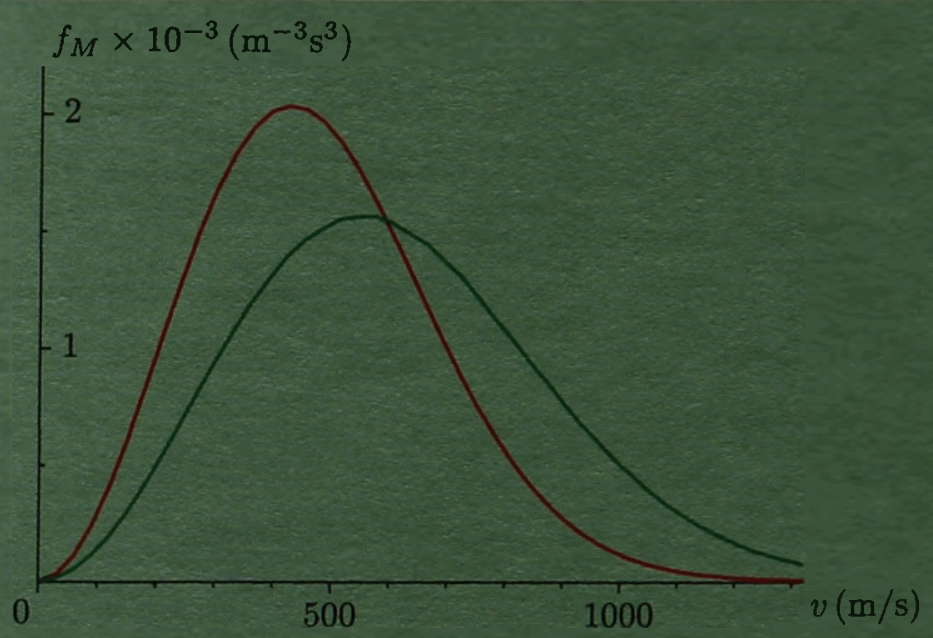
\includegraphics[width=0.4\linewidth]{mai_fig048.png}
   \captionof{figure}{Maxwellovo rozdělení rychlostí molekul dusíku pro teploty \(T_1 = 
                      \SI{300}{\kelvin}\) a \(T_2 = \SI{300}{\kelvin}\).
   \cite[s.~243]{Musilova2009MA1}
   \label{mai:fig048}}
  \par}
  
  Dokážete vyložit, proč jsme zvolili za \(\Delta\Omega\) celý objem slupky? Počítáme totiž 
  pravděpodobnost, že koncový bod vektoru rychlosti molekuly leží, zhruba řečeno, v kterémkoli 
  elementárním kvádříku \(\Delta v_x\Delta v_z\Delta v_z\) obsaženém ve slupce. A ta je součtem 
  pravděpodobností odpovídajících všem kvádříkům vytvářejícím slupku. Jedná se o pravděpodobnosti 
  navzájem neslučitelných jevů (pohybuje-li se molekula v jednom směru, nepohybuje se v jiném). 
  Hustota této pravděpodobnosti se nazývá \textbf{Maxwellovo rozdělení rychlostí}. Na rozdíl od 
  Gaussova rozdělení, popisujícího hustotu pravděpodobnosti pro jednotlivé složky rychlosti, je 
  nesymetrická vlivem faktoru \(v^2\). Obrázek \ref{mai:fig048} ukazuje funkci \(f_M(v)\) pro dvě 
  různé teploty \(T_2 > T_1\). Důležité hodnoty spjaté s tímto rozdělením jsou 
  \textbf{nejpravděpodobnější rychlost} \(v_p\), \textbf{střední rychlost} \(\langle v \rangle\) a 
  \textbf{střední kvadratická rychlost} \(\langle v^2 \rangle\). Platí
  \begin{align*}
    \der{f_M}{v}        &= 0\, \longrightarrow v_P = \sqrt{\dfrac{2kT}{m}},                      \\
    \langle v \rangle   &= \int_{-\infty}^{\infty}vf_M(v)\dd{v} = \sqrt{\dfrac{8kT}{\pi m}},     \\
    \langle v \rangle^2 &= \int_{-\infty}^{\infty}v^2f_M(v)\dd{v} = \dfrac{3kT}{m}.
  \end{align*}
\normalsize
\end{example}
      %---------------------------------------------------------------
  
  \section{Náhoda a zpracování měření}\label{mai:IchapIVsecIV}
    \subsection{Součet a součin náhodných veličin}
      Nyní vyřešíme ještě jeden důležitý problém. Víme již, že veličinu \(Y = f(X)\) lze popsat 
      stejnými pravděpodobnostmi jako veličinu \(X\). V řadě případů je však náhodná veličina \(Y\) 
      funkcí několika náhodných veličin \(X_1, X_2, \ldots, X_s\). Každá z nich má nějaké 
      rozdělení. Jaké potom bude rozdělení veličiny \(Y\)? Rozebereme jen dvě základní situace, z 
      nichž je ovšem možné „poskládat“ řadu případů složitějších. Půjde o situace, kdy náhodná 
      veličina bude součtem nebo součinem dvou náhodných veličin, pro jednoduchost značení 
      například \(U\) a \(V\), tedy \(Y = U + V\), \(Z = U \cdot V\). Předpokládejme nejprve, že 
      veličiny \(U\) a \(V\) jsou zcela nezávislé, tj. hodnoty veličiny \(U\) nejsou nijak 
      ovlivněny hodnotami veličiny \(V\) a naopak. Dejme tomu, že \(U\) a \(V\) mají rozdělení
      \begin{equation*}
        \left\lbrace (u_1, p_1), \ldots, (u_k, p_k) \right\rbrace, \qquad
        \left\lbrace (v_1, q_1), \ldots, (v_\ell, v_\ell) \right\rbrace
      \end{equation*}
      Veličiny \(Y = U + V\), resp. \(Z = U \cdot V\) tedy mohou nabývat hodnot \(\lbrace u_i + 
      v_\alpha\rbrace\), resp. \(\lbrace u_i v_\alpha\rbrace\) s pravděpodobnostmi \(p_iq_\alpha\). 
      Jevy \uv{Veličina \(U\) nabude hodnoty \(u_i\)} a \uv{veličina \(V\) nabude hodnoty 
      \(v_\alpha\)} jsou totiž nezávislé. Rozdělení veličin \(Y\) a \(Z\) je 
      \begin{equation*}
        \lbrace (u_i +v_\alpha, p_iq_\alpha)\rbrace,\, \text{resp.}\,
        \lbrace(u_iv_\alpha, p_iq_\alpha)\rbrace,\qquad 1\leq i\leq k,\quad 1\leq\alpha\leq\ell,
      \end{equation*}
      Pro jejich střední hodnoty dostáváme
      \begin{align*}
        \langle y \rangle 
          &= \sum_{i=1}^{k}\sum_{\alpha=1}^{\ell}(u_i + v_\alpha)p_iq_\alpha        \\
          &= \sum_{i=1}^{k}u_ip_i\left(\sum_{\alpha=1}^{\ell}q_\alpha\right) + 
             \sum_{\alpha=1}^{\ell}v_\alpha q_\alpha\left(\sum_{i=1}^{k}p_i\right)  \\
          &= \sum_{i=1}^{k}u_ip_i + \sum_{\alpha=1}^{\ell}v_\alpha q_\alpha         \\
        \langle z \rangle 
          &= \sum_{i=1}^{k}\sum_{\alpha=1}^{\ell}(u_i \cdot v_\alpha)p_iq_\alpha    \\
          &= \left(\sum_{i=1}^{k}u_ip_i\right)
             \left(\sum_{\alpha=1}^{\ell}v_\alpha q_\alpha\right) 
           = \langle u \rangle \langle v \rangle.
      \end{align*}
      Střední hodnota součtu, resp. součinu náhodných veličin je tedy součtem, resp. součinem jejich
      středních hodnot. Pro součet náhodných veličin platí tento výsledek i v případě, když nebudou
      nezávislé. V tak jednoduchý závěr jsme snad ani nedoufali! Hned uvidíme, jak jej lze využít.
      
      %--Jak číst výsledky studentské ankety aneb není průměr jako průměr----------
      % !TeX spellcheck = cs_CZ
\wikitextrule
\begin{example}\label{mai:exam071}
  \textbf{Jak číst výsledky studentské ankety aneb není průměr jako průměr}\newline\small
  Každý semestr na Masarykově univerzitě se uzavírá vyhodnocením velmi užitečné studentské ankety v 
  Informačním systému MU. Studenti hodnotí na jedenáctihodnotové stupnici (nula až deset bodů) 
  několik položek pro každý studijní předmět (obtížnost, zajímavost, srozumitelnost výkladu, 
  přístup učitele, rozmanitost literatury) a mohou doplnit i slovní komentáře. Na ty se učitelé 
  těší nejvíce, neboť díky anonymitě pisatelů se tak o sobě mohou dovědět leccos zajímavého. 
  Všimneme si však statistického zpracování ankety. U každého předmětu je pro danou položku 
  vypočtena průměrná bodová hodnota odpovědí a vyznačena na téže jedenáctihodnotové stupnici. Pro 
  porovnání je na stupnici vyznačen i takzvaný „fakultní průměr“. Každý přednášející může vidět svá 
  hodnocení a hodnocení svých kolegů, kteří mu vedou cvičení. Děkan má přístupové právo k celé
  statistice, a tak může porovnávat. Jednoho deštivého večera přestalo děkana bavit vyplňování 
  rektorátních formulářů a začal si výsledky ankety prohlížet. Zajímala jej zejména položka 
  „srozumitelnost výkladu“. Řekl si, že všem učitelům, kteří v této položce budou hodnoceni 
  nadprůměrně, zvýší osobní ohodnocení. Soubor předmětů je veliký, a tak děkan klikal a klikal. 
  Zjišťoval, že u veliké většiny předmětů leží průměrné hodnocení srozumitelnosti nad fakultním 
  průměrem. Jeho pocity byly smíšené. Na jedné straně se radoval, jakými jsou jeho podřízení 
  dobrými pedagogy, na druhé straně trnul, kolik to bude stát. Snad aby se raději vrátil 
  k protivným formulářům. Najednou v něm zahlodalo podezření i naděje, že není všechno v pořádku. 
  Jak je možné, že většina hodnocení leží nad průměrem? Kladné a záporné odchylky by se přece měly 
  kompenzovat. Zavolal proto na koberec proděkana pro informační technologie, aby se jej zeptal, co 
  je to „fakultní průměr“. Proděkan odpověděl takto: Máme soubor \(K\) předmětů \(\lbrace 
  X_\alpha\rbrace\), \(\alpha = 1, \ldots, K\). V předmětu \(X_\alpha\) vyplnilo anketu 
  \(N_\alpha\)  studentů, jednotlivé hodnoty odpovědí pro danou položku (srozumitelnost výkladu) 
  byly označeny \(\lbrace x_{\alpha,j}\rbrace\), \(j = 1, \ldots, N_\alpha\). Celkem přirozeně 
  předpokládáme, že váha odpovědi každého studenta je stejná, nezávisle na předmětu. Tato váha je
  rovna převrácené hodnotě celkového počtu studentů, kteří vyplnili anketu, tj. \(w = N^{-1}\), \(N 
  = N_1 + \ldots + N_k\). Fakultní průměr je proto dán vzorcem
  \begin{equation*}
    \langle x \rangle 
      = \sum_{\alpha=1}^{K}\sum_{j=1}^{N_\alpha}wx_{\alpha,j} 
      = \dfrac{1}{N}\sum_{\alpha=1}^{K}\left(\sum_{j=1}^{N_\alpha}x_{\alpha,j}\right)
      = \dfrac{1}{N}\sum_{\alpha=1}^{K}A_\alpha,
  \end{equation*}
  kde jsme označili \(A_\alpha = \sum_{j=1}^{N_\alpha}x_{\alpha,j}\). Děkan chvíli přemýšlel a 
  pravil: To vypadá docela logicky. Neměli bychom však počítat fakultní průměr tak, že vezmeme 
  průměrné hodnoty pro každý předmět a vypočteme jejich aritmetický průměr? Pak bychom dostali
  \begin{equation*}
    \langle \overline{x} \rangle
      = \dfrac{1}{K}\sum_{\alpha=1}^{K}\langle x_{\alpha}\rangle
      = \dfrac{1}{K}\sum_{\alpha=1}^{K}
        \left(\dfrac{1}{N_\alpha}\sum_{j=1}^{N_\alpha}x_{\alpha,j}\right)
      = \dfrac{1}{K}\sum_{\alpha=1}^{K}\dfrac{A_\alpha}{N_\alpha}.
  \end{equation*}
  Tento závěr se akademickým funkcionářům na první pohled nijak zvlášť nelíbil. Bylo totiž jasné, 
  že náhodné veličiny \(X_1, \ldots, X_k\) mají odlišná rozdělení. No jo, řekli si oba, musíme 
  počítat. My už ale počítat nemusíme, neboť jsme takový problém před chvílí vyřešili obecně. 
  Zjistili jsme totiž, že střední hodnota součtu náhodných veličin je rovna součtu středních 
  hodnot, bez ohledu na konkrétní rozdělení každé z veličin. Definujeme-li tedy náhodnou veličinu 
  \(Y\) jako aritmetický průměr veličin \(X_\alpha\), tj.
  \begin{align*}
    Y &= \dfrac{1}{K}\left(X_1 + \ldots + X_K\right),  \\
    \shortintertext{dostaneme}
    \langle y \rangle &= \dfrac{1}{K}\left(\langle x_1 \rangle +\ldots+\langle x_K \rangle\right).
  \end{align*}
  Tento výsledek se shoduje s hodnotou \(\langle \overline{x} \rangle\), kterou pro výpočet 
  „fakultního průměru“ navrhl děkan. Vypočteme-li součet odchylek hodnot \(\langle x_\beta 
  \rangle\) od \(\langle y \rangle\), dostaneme skutečně nulu:
  \begin{equation*}
    \sum_{\beta =1}^{K}\left(\langle x_\beta \rangle - \langle y \rangle\right)
      = \sum_{\beta =1}^{K}\left(\dfrac{A_\beta}{N_\beta} 
      - \dfrac{1}{K}\sum_{\alpha=1}^{K}\langle x_\alpha \rangle\right)
      = 0.
  \end{equation*}
  Zkusme se ještě zamyslet nad tím , jak použití „špatného“ fakultního průměru zkreslilo výsledky a 
  proč. Vypočtěme si rozdíl \(\Delta = \langle \overline{x} \rangle - \langle x \rangle\):
  \begin{equation*}
    \Delta = \langle \overline{x} \rangle - \langle x \rangle 
      = \dfrac{1}{K}\sum_{\alpha=1}^{K}\langle x_\alpha \rangle
      - \dfrac{1}{N}\sum_{\alpha=1}^{K}A_\alpha
      = \dfrac{1}{K}\sum_{\alpha=1}^{K}\langle x_\alpha \rangle
      - \dfrac{1}{N}\sum_{\alpha=1}^{K}N_\alpha\langle x_\alpha \rangle
      = \dfrac{1}{K}\sum_{\alpha=1}^{K}\langle x_\alpha\rangle\left(1 - K\dfrac{N_\alpha}{N}\right).
  \end{equation*}
  Platí přitom
  \begin{equation*}
    \sum_{\alpha=1}^{K}\left(1 - K\dfrac{N_\alpha}{N}\right) = 0.
  \end{equation*}
  Pokud by byl počet studentů, kteří vyplnili anketu, ve všech předmětech stejný, tj. \(N_\alpha = 
  \dfrac{N}{K}\) , byla by odchylka \(\Delta\) podle očekávání nulová. Stejná situace by nastala, 
  kdyby byly shodné všechny průměrné hodnoty \(\langle x_\alpha \rangle\). Je-li odchylka 
  \(\Delta\) kladná, je „nesprávný“ fakultní průměr \(\langle x \rangle\) nižší než \(\langle 
  \overline{x} \rangle\). Proto hodnocení jednotlivých předmětů vypadají příznivěji, právě tak, jak 
  to zjistil děkan. Odchylku \(\Delta\) posouvají do kladných hodnot předměty, které hodnotilo málo 
  studentů, a předměty, které měly vysoké hodnocení. Dobře je to vidět na příkladu dvou předmětů, 
  tj. pro \(K = 2\), kde vychází
  \begin{equation*}
    \Delta = \langle \overline{x} \rangle - \langle x \rangle 
           = \dfrac{N_2 - N_1}{2(N_2+N_1)}\left(\langle\overline{x}\rangle-\langle x\rangle\right).
  \end{equation*}
  
  Pro \(N_1\ll N_2\) a \(\langle x_1 \rangle  \gg \langle x_2 \rangle \) bude rozdíl \(\Delta\) 
  skoro polovina hodnoty \(\langle x_1 \rangle\)! U volitelných specializovaných předmětů, které si 
  vybírají jen poměrně malé počty studentů, kteří navíc mají o předmět opravdový zájem a hodnotí 
  jej proto většinou vyšším počtem bodů, je splněno obojí (malý počet hodnotících a vysoké bodové
  hodnocení). Je vidět, že při nesprávně zvoleném výpočtu srovnávací hodnoty (fakultního průměru) 
  mohou právě předměty, jejichž statistický význam je spíše okrajový, ovlivnit celkové hodnocení.
\normalsize
\end{example}
      %----------------------------------------------------------------------------
      
      Pro střední hodnotu součtu a součinu nezávislých náhodných veličin jsme získali velmi
      jednoduché výsledky:
      
      \begin{mdframed}[style=highlight]
        \begin{equation}\label{mai:eq070}
          \langle u + v \rangle = \langle u \rangle + \langle v \rangle\quad
          \langle uv \rangle    = \langle u \rangle \langle v \rangle.
        \end{equation}
      \end{mdframed}
      
      Dokážeme také určit rozptyl veličin \(Y = U + V\) a \(Z = U\cdot V\)? Pro rozptyl každé 
      náhodné veličiny platí obecný vztah (\ref{mai:eq061}). Použijeme jej pro naše konkrétní 
      případy:
      \begin{gather*}
        \begin{align*}
          D(U + V) &= \langle (u + v)^2 \rangle - \langle u + v \rangle^2                     \\
                   &= \langle u^2 + 2uv + v^2 \rangle - \left(\langle u \rangle^2 +
                      \langle 2uv \rangle + \langle v^2 \rangle\right)                        \\
                   &= \left(\langle u^2\rangle - \langle u \rangle^2\right)
                    + \left(\langle v^2\rangle - \langle v \rangle^2\right) = D(U) + D(V).
        \end{align*}
      \end{gather*}
      Pro rozptyl náhodné veličiny \(Z = U \cdot V\) dostaneme
      \begin{align*}
        D(Z)  &= \langle z^2\rangle - \langle z \rangle^2 
               = \langle u^2\rangle\langle v^2\rangle - \langle u \rangle^2 \langle v \rangle^2  \\
              &= \left[D(U) + \langle u^2\rangle\right]\left[D(V) + \langle v^2\rangle\right]
               - \langle u \rangle^2 \langle v \rangle^2                                         \\
              &= D(U)D(V) + \langle u \rangle^2D(V) + \langle v \rangle^2D(U).
      \end{align*}
      Pak
      \begin{mdframed}[style=highlight]
        \begin{equation*}
          \dfrac{D(z)}{ \langle z \rangle^2} = \dfrac{D(U)}{ \langle u \rangle^2} \cdot
            \dfrac{D(V)}{ \langle v \rangle^2} + \dfrac{D(U)}{ \langle u \rangle^2} +
            \dfrac{D(v)}{ \langle v \rangle^2}.
        \end{equation*}
      \end{mdframed}
      Při výpočtu jsme využili vztahu (\ref{mai:eq061}) a vztahů (\ref{mai:eq070}) pro střední 
      hodnotu součtu a součinu náhodných veličin. Pokud mají veličiny \(U\) a \(V\) shodný rozptyl 
      \(D(U) = D(V) = D\), pak je \(D(U + V) = 2D\). V případě součtu s veličin \(Y = X_1 + \cdots 
      + X_s\) se shodným rozptylem \(D\) resp. směrodatnou odchylkou \(\sigma\) dostáváme
      \begin{equation*}
        D(Y) = sD  \Rightarrow \sigma(y) = \sqrt{s}\sigma.
      \end{equation*}
      Znovu připomeňme, že všechny vztahy týkající se součtu a součinu náhodných veličin, které
      jsme zatím získali, platí za předpokladu, že výchozí veličiny, které sčítáme nebo násobíme, 
      jsou nezávislé.
      
      Aniž bychom se podrobněji zabývali vlastnostmi rozdělení závislých veličin, definujeme pro
      ně charakteristiky, které tuto závislost popisují. Nechť \(U\) a \(V\) jsou dvě libovolně 
      náhodné veličiny, ne nutně nezávislé. Míru jejich závislosti určují veličiny
      \begin{subequations}\label{mai:eq071}
        \begin{align}
          \sigma_{uv} 
            &= \langle (u - \langle u \rangle) (v - \langle v \rangle) \rangle,  \\
          \varrho_ {uv}
            &=\dfrac{\sigma(u)}{\sqrt{D(U)D(V)}} = \dfrac{\sigma(u)}{\sigma{D(u)\sigma(v)}}
        \end{align}
      \end{subequations}  
      zvané \textbf{kovariance} a \textbf{korelační koeficient} veličin \(U\) a \(V\). Platí 
      \(\varrho(uv) \leq 1\). Pro nezávislé veličiny vychází \(\sigma(uv) = 0\) a \(\varrho(uv) = 
      0\).
      
      %-- Rozptyl při Bernoulliově pokusu-----------------------------
      % !TeX spellcheck = cs_CZ
\begin{mdframed}[style=mdexam]
  \begin{example}\label{mai:exam072}
    \textbf{Rozptyl při Bernoulliově pokusu}\newline
    V příkladu \ref{mai:exam066} jsme se zajímali o střední hodnotu veličiny \(X\) definované jako
    počet zdarů při \(n\) opakováních Bernoulliova pokusu. Řekli jsme si, že střední hodnota této
    veličiny je \(np\) s tím, že důkaz lze provést přímo na základě definičního vztahu pro střední
    hodnotu matematickou indukcí. Výpočet rozptylu z definičního vztahu bychom jistě snadno dokázali
    zahájit, horší by však bylo dovést jej do konce. Stačí se podívat na začátek výpočtu
    \begin{align*}
      D(X) &= \sum_{j=0}^n \left(x_j - \langle x \rangle\right)^2p_j             \\
           &= \sum_{j=0}^n \left(j - np\right)^2\binom{n}{j}p^j(1 - p)^j,
    \end{align*}
    a nepochybujeme o tom, že tuto sumu nedokážeme spočítat snadno. Protože již však umíme zacházet
    se součtem náhodných veličin, můžeme využít účinného triku. Veličinu \(X\) si představíme jako
    součet
    \begin{equation*}
      X = U_1 + U_2 + \cdots + U_n,
    \end{equation*}
    kde každá z veličin \(U_j\) může nabývat dvou hodnot. Jedničky v případě, že při \(j\)-tém
    opakování pokusu nastal zdar, a nuly v případě, že nastal nezdar. Součet všech veličin \(U_j\)
    pro \(j = 1\) až \(j = n\) pak skutečně znamená celkový počet zdarů při \(n\) opakováních
    pokusu. Jestliže si uvědomíme, že pravděpodobnost zdaru při kterémkoli z opakování je \(p\) a
    pravděpodobnost nezdaru \((1 - p)\), ihned vidíme, že rozdělení každé z veličin \(U_j\) má tvar
    \(\lbrace(1, p), (0, 1 - p)\rbrace\). Platí tedy
    \begin{equation*}
      \langle u_j\rangle = 1\cdot p + 0 \cdot (1 - p) = p,
    \end{equation*}
    \begin{align*}
      D = D(U_j) &= \left( 1 - \langle u_j\rangle\right)^2p 
                  + \left( 0 - \langle u_j\rangle\right)^2(1 - p)   \\
                 &= p(1 - p)^2 + p^2(1 - p) = p(1 - p).
    \end{align*}
    Každé dvě veličiny \(U_i\), \(U_j\) jsou nezávislé, neboť jednotlivá opakování pokusu jsou
    nezávislá. Střední hodnota jejich součtu je: tedy \(np\) (a to souhlasí s informací v příkladu
    \ref{mai:exam066}) a pro rozptyl jejich součtu platí
    \begin{equation*}
      D(X) = nD = np(1 - p).
    \end{equation*}
    Celkově tedy dostáváme
    \begin{equation*}
      \langle x \rangle = np, \; \sigma(x) = \sqrt{np(1 - p)}.
    \end{equation*}
  \end{example}
\end{mdframed}
      %---------------------------------------------------------------
      
      %-- Rozptyl aritmetického průměru-------------------------------
      % !TeX spellcheck = cs_CZ
\begin{mdframed}[style=mdexam]
  \begin{example}\label{mai:exam073}
    \textbf{Rozptyl aritmetického průměru}\newline
    Již v úvodu odstavce o náhodných veličinách jsme konstatovali, že opakujeme-li v nezměněných
    podmínkách měření jisté fyzikální veličiny (délka závěsu kyvadla, proud procházející vodičem,
    napětí na vodiči, atd.), budeme díky náhodným vlivům dostávat pokaždé poněkud jiný výsledek.
    Říkáme, že měření je zatíženo náhodnými chybami. Výsledek získaný při každém opakování lze
    interpretovat jako hodnotu náhodné veličiny. Dejme tomu, že jsme provedli uměření fyzikální
    veličiny \(X\) a získali hodnoty \(x_1\) až \(x_n\) . V praktické situaci budou tyto hodnoty
    většinou navzájem různé, nemusí tomu tak však nutně být. Fyzikální veličinu chceme ovšem
    reprezentovat jediným údajem, a tím bude její střední hodnota, tj.
    \textbf{aritmetický průměr}
    \begin{equation*}
      \langle x \rangle = \dfrac{x_1 + x_2 + \cdots + x_n}{n}.
    \end{equation*}
    Rozptyl veličiny \(X\) je dán vztahem
    \begin{align*}
      D &= D(X)                                                             \\
        &= \dfrac{\left(x_1 - \langle x \rangle\right)^2 + 
                  \left(x_2 - \langle x \rangle\right)^2 + \cdots +
                  \left(x_n - \langle x \rangle\right)^2}{n}.
    \end{align*}
    Víme, že směrodatná odchylka \(\sigma( x ) = \sqrt{D(X)}\) určuje, nakolik jsou jednotlivé
    výsledky měření v průměru odchýleny od střední hodnoty, charakterizuje tedy přesnost každého
    opakování měření. Podívejme se na celou úlohu z jiné strany: Představme si, že sledujeme \(n\)
    po dvou nezávislých náhodných veličin \(X_1\) až \(X_n\) se shodnou střední hodnotou \(\langle
    x_j \rangle = \langle x \rangle\) a shodnou směrodatnou odchylkou \(\sigma(x_j) = \sqrt{D},\, 1
    \leq j \leq n\). Aritmetický průměr těchto veličin,
    \begin{equation*}
      \langle \Xi \rangle = \dfrac{X_1 + X_2 + \cdots + X_n}{n}.
    \end{equation*}
    je tedy rovněž náhodnou veličinou. Pro jeho střední hodnotu, rozptyl a směrodatnou odchylku
    platí
    \begin{align*}
      \langle \xi \rangle 
                  &= \dfrac{n\langle x \rangle}{n}, \\
      D(\Xi)      &= \dfrac{1}{n^2}\cdot D(X_1 + \cdots + X_n)=\dfrac{nD^2}{n^2}=\dfrac{D}{n}, \\
      \sigma(\xi) &= \dfrac{\sigma(x)}{\sqrt{n}}.
    \end{align*}
  \end{example}
\end{mdframed}
      %---------------------------------------------------------------
      
      Můžeme tedy říci, že aritmetický průměr všech výsledků měření dané fyzikální veličiny je
      \(\sqrt{n}\)-krát přesnější než jednotlivý výsledek měření. Jakkoli se toto konstatování zdá 
      intuitivně zřejmé, je třeba je používat s opatrností.
      
      Především je třeba mít na mysli, co toto konstatování znamená. Jeho charakter je totiž
      opět jen pravděpodobnostní. Jestliže jsou jednotlivá měření prováděna za stejných podmínek,
      jsou rozdělení veličin \(X_1\) až \(X_n\) funkcemi téhož typu. Tyto veličiny mají také 
      stejnou střední hodnotu \(\langle x \rangle\) a směrodatnou odchylku \(\sigma\). Také 
      pravděpodobnost, že při měření padne hodnota veličiny \(X_j\) do intervalu \((\langle x 
      \rangle - \sigma, \langle x \rangle + \sigma)\), je pro všechna \(j\) prakticky stejná. 
      Označme ji \(P_\sigma\).  Se stejnou pravděpodobností nabude aritmetický průměr \(\Xi\) 
      hodnoty v intervalu určeném svou směrodatnou odchylkou. Ta je však \(\sqrt{n}\)-krát menší. V 
      tomto smyslu jsou hodnoty aritmetického průměru \uv{\(\sqrt{n}\)-krát méně rozptýleny} kolem 
      střední hodnoty \(\langle\xi \rangle\) než hodnoty náhodných veličin \(X_j\) kolem svých 
      středních hodnot \(\langle x \rangle\).
      
      Dalším problémem může být splnění výchozích předpokladů, které vedly ke vztahu pro
      směrodatnou odchylku aritmetického průměru. Ukážeme to na následujícím příkladu.
      
      %-- Jak přesně lze změřit čínského císaře?----------------------
      % !TeX spellcheck = cs_CZ
\wikitextrule
\begin{example}\label{mai:exam075}
  \textbf{Ověření Ohmová zákona}\newline\small

\normalsize
\end{example}
      %---------------------------------------------------------------
      
      %-- Záhada přijímací zkoušky aneb k čemu může posloužit distribuční funkce-----
      % !TeX spellcheck = cs_CZ
\begin{mdframed}[style=mdexam]
  \begin{example}\label{mai:exam075}
    \textbf{Záhada přijímací zkoušky aneb k čemu může posloužit distribuční funkce?}\newline
    Mohlo by se zdát, že distribuční funkce je jen teoretický pojem a že v praktických situacích ji
    těžko využijeme. Podstatné je přece pravděpodobnostní rozdělení náhodné veličiny a distribuční
    funkce je z něj jen jaksi odvozena sčítáním pravděpodobností (u diskrétního rozdělení) nebo
    integrací (u rozdělení spojitého). Přesvědčíme se, že existují velmi realistické případy, kdy
    distribuční funkce přináší věrohodnější informaci o náhodné veličině než samotné rozdělení.
    
    Na Masarykově univerzitě musí každý uchazeč o studium, ať již se hlásí na přírodovědeckou,
    právnickou, lékařskou či jinou fakultu, absolvovat Test studijních předpokladů. Jedná se o
    všeobecný test, zaměřený na zjišťování úrovně všech schopností uchazeče, které jsou potřebné pro
    univerzitní studium, například analytického myšlení, verbálních schopností, numerického myšlení,
    geometrické představivosti, atd. Pro nás však v tu to chvíli není podstatný obsah testu, ale
    způsob zpracování jeho výsledků a vyhodnocení pořadí uchazečů. Test skládá kolem třiceti tisíc
    studentů. Není tedy možné technicky zajistit, aby proběhl v jediné variantě v jednom dni. K
    dispozici je proto osm variant testu, každou variantu řeší tři až čtyři tisíce studentů. Test má
    \num{80} otázek, základním údajem pro zpracování jeho výsledků je počet správných odpovědí
    každého studenta. Pokud bychom označili jako \(i\) počet správných odpovědí (\(i \in\lbrace0, 1,
    2, \ldots, 80\rbrace\)) v kterékoli variantě a \(\mathcal{N}_i\) počet studentů, kteří dosáhli
    právě \(i\) správných odpovědí, dostaneme náhodnou veličinu \(X_i\), kterou bychom mohli nazvat
    „počet správných odpovědí“, pro celou univerzitu. Její rozdělení by mělo tvar
    \begin{equation*}
      \lbrace(i,p_i)\rbrace,\quad\text{kde}\qquad p_i = \dfrac{\mathcal{N}_i}{\mathcal{N}}, \quad
      \mathcal{N} = \sum_{i=0}^{80}\mathcal{N}_i
    \end{equation*}
    A zde je malý „kámen úrazu“. A by bylo možné sestavit opravdu „univerzální pořadí“, musely by
    být všechny varianty testu ekvivalentní z hlediska obtížnosti. To znamená, že kdyby kterýkoli
    student vyplnil za stejných podmínek všechny varianty, dosáhl by v každé z nich stejného počtu
    správných odpovědí s pravděpodobností velmi blízkou jedné. Skutečnost je však principiálně
    taková, že u sebelépe promyšleného a sestaveného testu se jednotlivé varianty budou mírně, v
    rámci statistických, a tedy již neodstranitelných, odchylek lišit. Tato odlišnost se nepozná
    předem, ale až po zpracování výsledků všech variant. Použít pro stanovení pořadí uchazečů
    rozdělení náhodné veličiny \(X\) \emph{= počet správných odpovědí je tedy nespravedlivé}.
    Student, který řešil variantu „statisticky obtížnější“, by v pořadí skončil s horším umístěním,
    než student, který je stejně schopný, avšak měl to štěstí, že na něj připadla varianta
    „statisticky méně obtížná“. Skutečně, kdybychom sestavili grafy rozdělení náhodných veličin
    \(X^{(\alpha)}\) \emph{= počet správných odpovědí v \(\alpha\)-té variantě},
    \begin{equation*}
      \lbrace(i,p_i^{(\alpha)})\rbrace,\quad\text{kde}\; 
      p_i^{(\alpha)} = \dfrac{\mathcal{N}_i^{(\alpha)}}{\mathcal{N}^{(\alpha)}}, \quad
      \mathcal{N}^{(\alpha)} = \sum_{i=0}^{80}\mathcal{N}_i^{(\alpha)}
    \end{equation*}
    zjistili bychom, že se mírně liší. (V předchozím zápisu značí \(\mathcal{N}_i^{(\alpha)}\) počet
    studentů, kteří odpověděli správně na \(i\) otázek \(\alpha\)-té varianty
    \(\mathcal{N}^{(\alpha)}\) je počet všech studentů, kteří tuto variantu řešili.) Střední hodnoty
    i mediány náhodných veličin se i při vynikající shodě obtížnosti všech variant mohou lišit v
    rozmezí jedné až dvou správných odpovědí. A s ohledem na skutečnost, že každou variantu řeší
    obrovský počet studentů, až čtyři tisíce, je zřejmé, že tento rozdíl může poněkud „zamíchat
    “pořadím, zejména v blízkosti mediánu, kde se týká třeba i tří stovek studentů v každé variantě.
    Situaci dokládá obrázek \ref{mai:fig049}. Jak tedy zařídit, abychom dostali spravedlivé pořadí?
    Jediný rozumný způsob, jak minimalizovat vliv statistických odchylek obtížnosti jednotlivých
    variant, je nehodnotit studenty podle absolutního počtu správných odpovědí, ale nějak je
    porovnat mezi sebou. Budeme při tom předpokládat, že rozložení schopností studentů je ve všech
    osmi skupinách, které řeší osm daných variant, stejné. Řeknete si - zase nějaké další
    předpoklady. To je jako z bláta do louže. Předpoklad o stejném rozložení schopností studentů v
    tak velkých skupinách, jako jsou ty naše, je však mnohem realističtější než předpoklad o
    dokonalé shodě obtížnosti variant testu. Budeme se jej proto držet. Každému studentovi
    přisoudíme číslo, které informuje o tom, kolik řešitelů dané varianty bylo horších nebo stejně
    dobrých jako on, tj. mělo nižší nebo stejný počet správných odpovědí. Z matematického hlediska
    to znamená přejít v každé variantě od rozdělení k distribuční funkci. Věnujme se nyní tomuto
    přepočtu podrobněji jak pro diskrétní rozdělení náhodné veličiny \(X^{(\alpha)}\), které
    odpovídá skutečné situaci, tak pro zajímavost i pro rozdělení spojité. V dalším budeme vždy
    zpracovávat výsledky jedné varianty, upustíme proto od vyznačování indexu \(\alpha\).

    {\centering
    \captionsetup{type=figure}
    \luafigure[0.8]{mai_fig049.png}
    \captionof{figure}{Rozdělení pro dvě varianty testu,
    \cite[s.~252]{Musilova2009MA1}
    \label{mai:fig049}}
    \par}
    
    \textbf{Diskrétní rozdělení}
      \begin{itemize}
        \item \emph{Zadání:} Skupina \(N\) studentů řeší jednu variantu testu. Test má \(Q\) otázek.
              Za každou správnou odpověď je přidělen jeden výchozí bod. Získáváme rozdělení
              \begin{gather*}
                \left\lbrace\left(i, \dfrac{N_i}{N} \right)\right\rbrace, \;
                i\in\lbrace0, 1, 2, \ldots, Q\rbrace, \;
                \sum_{i=0}^{Q}N_i = N 
              \end{gather*}
              kde \(i\) je počet výchozích bodů a \(N_i\) počet studentů, kteří získali \(i\) bodů.
              Distribuční funkce tohoto rozdělení
              \begin{gather*}
                F(x) = \dfrac{1}{N}\sum_{i=0}^{j}N_i\;\text{ pro }\;
                j\leq x < j+1, \; x\in\left[0,\infty\right)
              \end{gather*}
              Pro uchazeče, který získal \(j\) bodů, mají význam následující hodnoty:
              \begin{itemize}
                \item \(F(x)    x \in \left[j, j+1\right)\): poměrný počet uchazečů, kteří získali
                      počet výchozích bodů nižší nebo shodný s daným uchazečem,
                \item \(NF(x)   x \in \left[j, j+1\right)\): absolutní počet uchazečů, kteří získali
                      počet výchozích bodů nižší nebo shodný s daným uchazečem,
                \item \(100F(x) x \in \left[j, j+1\right)\): absolutní počet uchazečů, kteří získali
                      počet výchozích bodů nižší nebo shodný s daným uchazečem,
              \end{itemize}
        \item Hodnoty distribuční funkce můžeme získat z následující tabulky:
        
              {\centering
                \resizebox{0.8\textwidth}{!}{%
                \begin{tabular}{c|c}
                          interval \(x\)     &  \(NF(x)\)         \\ \hline
                  \(\left[0,1\right)\)       &  \(N_0\)           \\ 
                  \(\left[1,2\right)\)       &  \(N_0 + N_1\)     \\ 
                  \(\cdots\)                 &  \(\cdots\)        \\
                  \(\left[j,j+1\right)\)     &  \(N_0 + N_1 + \cdots + N_j\) \\ 
                  \(\cdots\)                 &  \(\cdots\) \\
                  \(\left[Q-1,Q\right)\)     &  \(N_0 + N_1 + \cdots + N_{Q-1}\) \\ 
                  \(\left[Q,\infty\right)\)  &  \(N_0 + N_1 + \cdots + N_{Q} = N\) 
                \end{tabular}}
              \par}
        \item Přepočet hodnocení uchazečů tak, aby nová stupnice byla opět v rozsahu mezi nulou a
              \(Q\) a aby nové hodnocení bylo opět celočíselné, je následující:
              \begin{equation*}
                y =QF(x), \quad 0\leq F(x) \leq 1, \Rightarrow y \in[0,Q].
              \end{equation*}
              Uchazeči se ziskem \(i\) výchozích bodů náleží hodnota \(y = QF(x)\) právě když i\(
              \in \left[i, i + 1\right)\), tj. \(y_i = Q F(i)\). Tato hodnota není obecně
              celočíselná. Zaokrouhlení se provede ve prospěch uchazeče, tedy vždy nahoru. Výsledný
              převodní vzorec je
              \begin{equation*}
                \begin{multlined}
                  \text{výchozí body } i \longrightarrow\text{ nové body }  \\ 
                  \shoveleft[1cm]Y_i: Y_i = [y_i] + 1 = [QF(i)] + 1,
                \end{multlined}
              \end{equation*} 
              kde \([a]\) značí celočíselnou část čísla \(a\), tedy například \([\num{23.05}] =
              [\num{23.48}] = [23,89] = 23\)
        \item Zaveďme novou náhodnou veličinu \(Z\) s rozdělením \(\left\lbrace(z_\alpha,
              M_\alpha)\right\rbrace\): Označme \(z_1, z_2, \ldots, z_\alpha, ...,\) \(z_S\)
              navzájem různé hodnoty ze souboru \(\lbrace Y_i\rbrace, i = 0, 1, 2, \ldots, Q\)
              řazené vzestupně. Její rozdělení udává kterákoli z následujících tabulek:

              {\centering
                \resizebox{0.9\textwidth}{!}{%
                \begin{tabular}{c|c}
                          hodnota                       &  četnost         \\
                          \hline
                  \(z_1 = Y_0 = Y_1 = \cdots Y_{i_1}\)  & \(M_1 = N_0 + N_1 + \cdots + N_{i_1}\)  \\ 
                  \(Z_2 = Y_{i_1+1} = \cdots Y_{i_2}\)  & \(M_2 = N_{i_1+1} + \cdots + N_{i_2}\)  \\ 
                  \(\cdots\)                            & \(\cdots\)                              \\
                  \(Z_S = Y_{i_{S-1}+1}=\cdots Y_{i_S}\)& \(M_S = N_{i_{S_1}+1}+\cdots+N_{i_S}\)   
                \end{tabular}}
              \par}

              {\centering
                \resizebox{0.9\textwidth}{!}{%
                \begin{tabular}{c|c}
                          hodnota                        &  četnost         \\
                          \hline
                  \(z_1 = Y_0 = Y_1 = \cdots Y_{i_1}\)   &  \(M_1 = NF(i_1)\)              \\
                  
                  \(Z_2 = Y_{i_1+1} = \cdots Y_{i_2}\)   &  \(M_2 = N[F(i_2) - F(i_1)]\)  \\ 
                  \(\cdots\)                             &  \(\cdots\)                     \\
                  \(Z_S = Y_{i_{S-1}+1}=\cdots Y_{i_S}\) & \(M_S = N[F(i_S) - F(i_{S-1})]\)   
                \end{tabular}}
              \par}
              kde \(i_1 < i_2 < \ldots < i_{S-1} < i_S, i_S = Q\) (Vzhledem k zaokrouhlování nahoru
              není žádná bodová hodnota \(Y_i\) nulová.) I když skutečné rozdělení při zpracování
              výsledků testů je diskrétní, ukažme si, jak by vypadal analogický postup u rozdělení
              spojitého, kde je početní zpracování názornější.
      \end{itemize}
    
    \textbf{Spojité rozdělení}
      \begin{itemize}
        \item \emph{Zadání:} Je dáno rozdělení četností \(n(x) \leq 0,\, x \in [0, Q]\).
        \item Normovací podmínka a distribuční funkce jsou
              \begin{equation*}
                \int_{0}^{Q}n(x)\dd{x} = N, \quad 
                F(x) = \dfrac{1}{n}\int_{0}^{x}n(\xi)\dd{\xi},                
              \end{equation*}
              kde \(0 \leq F(x) \leq 1.\)
        \item Označme \(z = QF(x)\), tedy \(z \in [0, Q]\), novou náhodnou veličinu. (Uvědomme si,
              že \(z\) je rostoucí funkcí proměnné \(x\)). Označme její rozdělení \(\nu(z)\). Její
              distribuční funkce je
              \begin{align*}
                \Phi(z) &= \int_{0}^{z}\nu(\zeta)\dd{\zeta} 
                         = \int_{0}^{x(z)}\dfrac{n(\xi)}{N}\dd{\xi}          \\
                        &= F\left(F^{-1}(z/Q)\right) 
                        = \dfrac{z}{Q}, \quad
                \nu(z) = \dfrac{1}{Q}.
              \end{align*}
        \item Rozdělení je konstantní s mediánem i střední hodnotou \(Q/2\). Takové rozdělení se
              nazývá rovnoměrné.
      \end{itemize}
  \end{example}
\end{mdframed}
      %------------------------------------------------------------------------------
      
    \subsection{Který výsledek je ten pravý?}
      První věc, kterou budete dělat ve fyzikálním praktiku, bude zjišťování průměrné hustoty 
      materiálu, z něhož je vyroben kovový váleček. Budete váleček vážit, abyste určili jeho 
      hmotnost,a měřit jeho výšku a průměr, abyste mohli vypočítat jeho objem. Hustotu stanovíte 
      jako podíl hmotnosti a objemu. Jedná se stále o jeden a týž váleček, jehož průměrná hustota 
      má za daných podmínek (stálá teplota, váleček se nedeformuje, apod.) stále stejnou „správnou“ 
      hodnotu, kterou však neznáme. (Nezná ji ani učitel v praktiku, i když se tak tváří.) Změří-li 
      hustotu válečku všichni studenti ve skupině, každý jen jednou, získá se řada různých hodnot. 
      Která z nich je ta správná? Není vyloučeno, a je to dokonce velmi pravděpodobné, že žádná. A 
      mohli bychom pomocí nich správnou hodnotu určit nebo se k ní alespoň přiblížit? Možné by to 
      bylo, pokud bychom zaručili, že všechny výsledky získané jednotlivými studenty jsou „stejně 
      hodnotné“. Znamenalo by to, že bychom museli vyloučit hrubé a systematické chyby, které by 
      vznikly třeba tak, že by někteří studenti vážili na vadných vahách, někteří by měli špatné 
      měřítko, popřípadě by odečítali údaj „zboku“, takže by byl zkreslený, nebo by se dokonce 
      zmýlili při odečítání údaje. Museli bychom také zaručit, že náhodné vlivy, které ovlivňují 
      měření, zatěžují je náhodnými chybami a v principu je nelze odstranit, byly při všech 
      měřeních stejné. U různých studentů si tím však nemůžeme být jisti (vzpomeňte si na měření 
      čínského císaře), proto budeme raději postupovat tak, že jeden pečlivý student provede větší 
      počet měření třeba výšky válečku, která je pro určení hustoty potřebná. Dejme tomu, že bude 
      měřit milimetrovým měřítkem a bude odhadovat s přesností na půl milimetru. Jeho údaje tedy 
      mohou mít tvar \SI{33.0}{\mm}, \SI{34.5}{\mm}, atd. Získá takto za stejných podmínek třeba 
      dvacet nebo i padesát hodnot, ale co teď s nimi? Jak určit hodnotu, která se bude nejvíce 
      blížit správné hodnotě výšky válečku? (Dalo by se jistě diskutovat i o tom, co je to správná 
      hodnota. Pro tuto chvíli však předpokládejme, že taková hodnota skutečně existuje, neboť 
      váleček je opravdu válcem, je vysoustružen pečlivě, přesněji, než jsme schopni jej měřit, při 
      měření se nemění teplota, váleček není dáván do lisu a deformován, ani upravován tak, že by 
      se měnila jeho hmotnost.) Předpokládejme, že správná hodnota výšky válečku je \(x\) a že 
      student naměřil hodnoty \(\lbrace x_1, X_2, \ldots, x_n\rbrace\), mezi nimiž mohou být 
      pochopitelně i některé hodnoty stejné. Odchylky jeho měření od správné hodnoty jsou
      \begin{equation*}
        \lbrace \varepsilon_1, \varepsilon_2, \ldots, \varepsilon_n\rbrace, \qquad
        \varepsilon_i = x_i - x, \qquad i = 1, 2, \ldots, n.
      \end{equation*}
      I kdybychom správnou hodnotu \(x\) znali, nedokázali bychom předpovědět, nakolik se od ní při
      jednotlivém měření odchýlíme. Můžeme, se však zajímat o to, jaká je pravděpodobnost, že
      hodnota, o kterou bude měření od správné hodnoty odkloněno, bude ležet v určitém intervalu.
      Odchylky \(\varepsilon_i\) lze totiž interpretovat jako hodnoty náhodné veličiny. Abychom 
      mohli požadované pravděpodobnosti určit, potřebujeme znát rozdělení této veličiny. Označme ji 
      \(\varepsilon\) a odpovídající hustotu pravděpodobnosti \(\mathcal{w}(\varepsilon)\). Toto 
      rozdělení je za určitých podmínek \textbf{rozdělením normálním}, splňuje tedy vztah 
      (\ref{mai:eq069}). Zkusme se o tom přesvědčit. Zvolme podmínky měření tak, aby byly ve hře 
      jen náhodné chyby způsobené \(m\) nezávislými vlivy. Každý z nich hodnotu měření
      odchýlí od \(x\) o stejně velkou hodnotu \(\alpha\), kladnou nebo zápornou, s 
      pravděpodobností \num{0.5}. Schéma této úvahy je na obrázku \ref{mai:fig050}. Výsledná 
      odchylka naměřené hodnoty \(x_i\) od hodnoty správné s jistotou leží v intervalu \((-m\alpha, 
      m\alpha)\) a může nabývat pouze hodnot celých násobků \(\alpha\). Při uplatnění jednotlivého 
      „chybového“ vlivu vzniká, jak jsme již řekli, kladná nebo záporná odchylka o velikosti 
      \(\alpha\). Vznik odchylky \(+\alpha\) nazveme zdarem, vznik odchylky \(-\alpha\) nezdarem.
      
      \luagraphic[1]{mai_fig050.png}{Vznik kladných a záporných odchylek při měření s \(m\) vlivy. 
      \cite[s.~255]{Musilova2009MA1}}{mai:fig050}
     
      Mohlo by tomu být i naopak, slova „zdar“ a „nezdar“ zde nemají svůj obvyklý význam, jde
      pouze o to, že díky nim můžeme hned uvidět souvislost s Bernoulliovým pokusem a tedy
      i s Bernoulliovým rozdělením. Při \(j\) kladných a \(m - j\) záporných odchylkách je měření od
      správné hodnoty odkloněno o
      \begin{equation*}
        j\alpha + (m - j)(-\alpha) = (2j - m)\alpha
      \end{equation*}
      s pravděpodobností
      \begin{equation*}
        p_j = \binom{m}{j}p^j(1 - p)^{m - j} = 2^{-m}.
      \end{equation*}
      Střední hodnota náhodné veličiny \(\varepsilon\) je nulová. Skutečně, v příkladu 
      \ref{mai:exam066} jsme zjistili, že střední hodnota veličiny \(Y\) nabývající hodnot \(y_j = 
      j\) s Bernoulliovým rozdělením je \(\langle y \rangle = mp\), střední hodnota veličiny \((2j 
      - m)\) a pak musí být \((2mp - m)\alpha\). Pro \(p = \num{0.5}\) je tato hodnota nulová.
      Pro velká \(m\) lze Bernoulliovo rozdělení nahradit rozdělením normálním (obr. 3.8), a proto 
      má náhodná veličina \(\varepsilon\) hustotu pravděpodobnosti tvaru (\ref{mai:eq069}), tj.
      \begin{equation*}
        \mathcal{w}(\varepsilon) = 
        \dfrac{1}{\sigma\sqrt{2\pi}}\exp\left(\dfrac{-\varepsilon^2}{2\sigma^2}\right).   
      \end{equation*}

      \luagraphic[0.8]{mai_fig051.png}{Normální rozdělení jako limitní případ Bernoulliova 
      \cite[s.~256]{Musilova2009MA1}}{mai:fig051}
    
      Vraťme se nyní k otázce zpracování naměřených hodnot \(\lbrace x_1, \ldots, x_n\rbrace\) 
      výšky válečku. Jejich odchylky od správné hodnoty jsou \(x_1 - x\) až \(x_n - x\). Na místě 
      neznámé správné hodnoty \(x\) si nyní představme nějakou proměnnou, označme ji 
      \(\varepsilon\). Budeme se snažit určit její hodnotu \(\varepsilon_0\) tak, aby 
      pravděpodobnost, že odchylky jednotlivých měřených hodnot od \(\varepsilon_0\) padnou 
      současně do intervalů
      \begin{equation*}
        \begin{multlined}
          \left(\varepsilon_1 - \dfrac{\dd{\varepsilon_1}}{2}, 
                \varepsilon_1 + \dfrac{\dd{\varepsilon_1}}{2}
          \right),
          \left(\varepsilon_2 - \dfrac{\dd{\varepsilon_2}}{2}, 
                \varepsilon_2 + \dfrac{\dd{\varepsilon_2}}{2}
          \right), \cdots, \\
          \shoveleft[0.5cm]\left(\varepsilon_n - \dfrac{\dd{\varepsilon_n}}{2}, 
                                \varepsilon_n + \dfrac{\dd{\varepsilon_n}}{2}
                          \right),          
        \end{multlined}
      \end{equation*}
      byla maximální. Pro tuto pravděpodobnost v závislosti na \(\xi\) platí
      \begin{gather}
        \begin{aligned}
          \dd{W} &= \dd{\mathcal{w}(\varepsilon_1)}\cdots\dd{\mathcal{w}(\varepsilon_n)} \nonumber\\
                 &= \dfrac{1}{\sigma\sqrt{2\pi}}
                    \exp\left(-\dfrac{(x_1 - \xi)^2 + \cdots + (x_n - \xi)^2}{2\sigma^2}
                        \right)\dd{\varepsilon_1}\cdots\dd{\varepsilon_n}.      \label{mai:eq072}
        \end{aligned}
      \end{gather}
      (Víte proč je ve vztahu (\ref{mai:eq072}) součin pravděpodobností?) Tato pravděpodobnost bude 
      maximální, bude-li hodnota exponentu minimální. Z podmínky
      \begin{equation*}
        (x_1 - \xi)^2 + \cdots + (x_n - \xi)^2 = \text{min}
      \end{equation*}
      dostáváme derivací podle \(\xi\) požadavek
      \begin{equation*}
        2(x_1 - \xi) + \cdots + 2(x_n - \xi) = 0 \Rightarrow \xi_0 = 
        \dfrac{1}{n}\sum_{i=1}^{n}x_j = \langle x \rangle.
      \end{equation*}
      Vidíme, že veličina, která charakterizuje míru odchýlení naměřených hodnot od \(\xi\), je 
      minimální, zvolíme-li za \(\xi\) aritmetický průměr naměřených hodnot. Pozor, zjištěný 
      výsledek znamená právě jen konstatovanou skutečnost: Při dosazení aritmetického průměru za 
      proměnnou \(\xi\) bude pravděpodobnost, že odchylky jednotlivých měření od \(\xi\) budou 
      ležet v uvažovaných intervalech, maximální. Neznamená to, že správnou hodnotou veličiny \(X\) 
      je aritmetický průměr měření \(x_1, X_2, \ldots, x_n\). Správnou hodnotu ze souboru měření 
      prostě nezjistíme, avšak aritmetický průměr je jí blízký s vysokou pravděpodobností. Jaká je 
      tato „blízkost“ a její pravděpodobnost konkrétně? Hned uvidíme. Správnou hodnotu výšky 
      válečku \(x\) sice neznáme, ale víme, že náhodná veličina \(\varepsilon\), jejíž hodnoty jsou 
      odchylkami výsledků měření od této (neznámé) správné hodnoty, se řídí normálním rozdělením s 
      nulovou střední hodnotou. Potřebujeme stanovit další důležitý parametr tohoto rozdělení, 
      směrodatnou odchylku \(\sigma\). Tu lze vyjádřit velmi jednoduše. Je totiž střední hodnotou 
      náhodné veličiny \(\varepsilon^2\), tedy aritmetickým průměrem čtverců odchylek 
      \(\varepsilon_i\): 
      \begin{equation*}
        \sigma^2 = D(\varepsilon) = \dfrac{1}{n}\sum_{i=1}^{n}\varepsilon_i^2.
      \end{equation*}
      Ať je však tento vzorec jakkoli jednoduchý, k čemu může sloužit, nedokážeme-li jej vyčíslit?
      Když přece neznáme správnou hodnotu \(x\), nemáme k dispozici ani hodnoty \(\varepsilon_i\). 
      Ani tato kaše však není tak horká, jak se zdá: Odchylku výsledku \(i\)-tého měření od 
      aritmetického průměru označme \(\delta_i = x_i - \langle x \rangle\), přičemž jsme již dříve 
      označili jako \(\varepsilon_i= x_i - x\) odchylku výsledku \(i\)-tého měření pd správné 
      hodnoty. Platí
      \begin{equation*}
        \sum_{i=1}^{n}\varepsilon_i = \sum_{i=1}^{n}(x_i - x) \Rightarrow 
        \sum_{i=1}^{n}x_i = \sum_{i=1}^{n}\varepsilon_i + nx, 
      \end{equation*}
      odkud 
      \begin{equation*}
        \langle x \rangle = x + \dfrac{1}{n}\sum_{i=1}^{n}\varepsilon_i.
      \end{equation*}
      Pak dostaneme
      \begin{equation*}
        \delta_i = (x_i - x) - \dfrac{1}{n}\sum_{i=1}^{n}\varepsilon_i 
                 = \varepsilon_i - \dfrac{1}{n}\sum_{j=1}^{n}\varepsilon_j.
      \end{equation*}
      Součet čtverců odchylek \(\delta_i\) je
      \begin{align*}
        \sum_{i=1}^{n}\delta_i^2 
          &= \sum_{i=1}^{n}\left(\varepsilon_i - 
             \dfrac{1}{n}\sum_{j=1}^{n}\varepsilon_j\right)^2 \\
          &= \sum_{i=1}^{n}\varepsilon_i^2 - 
             \dfrac{2}{n}\sum_{i=1}^{n}\sum_{j=1}^{n}\varepsilon_i\varepsilon_j + 
             \dfrac{1}{n^2}\sum_{i=1}^{n}\left(\sum_{j=1}^{n}\varepsilon_j\right)^2     \\
          &= \sum_{i=1}^{n}\varepsilon_i^2 - 
             \dfrac{1}{n}\left(\sum_{j=1}^{n}\varepsilon_j\right)^2                     
             \doteq \left(1 - \dfrac{1}{n}\right)\sum_{i=1}^{n}\varepsilon_i^2.
      \end{align*}
      Při poslední úpravě jsme pro získání výsledného přibližného vyjádření součtu čtverců odchylek
      \(\delta_i\) použili následující úvahy:
      \begin{equation*}
        \left(\sum_{j=1}^{n}\varepsilon_j\right)^2 = \sum_{i=1}^{n}\varepsilon_i^2 + 
        2\sum_{i=1}^{n}\sum_{j>1}\varepsilon_i\varepsilon_j \doteq \sum_{i=1}^{n}\varepsilon_i^2,
      \end{equation*}
      neboť při rovnocenném zastoupení kladných a záporných odchylek je druhý sčítanec, obsahující
      součiny \(\varepsilon_i\varepsilon_j\), zanedbatelný proti prvnímu. Nakonec tedy dostáváme
      \begin{equation*}
        \sum_{i=1}^{n}\delta_i^2 \doteq \dfrac{n-1}{n}\sum_{i=1}^{n}\varepsilon_i^2 = (n-1)\sigma^2.
      \end{equation*}
      Protože odchylky \(\delta_i\) již z daného souboru měření určit můžeme (jsou to odchylky 
      jednotlivých měření od jejich aritmetického průměru), získali jsme alespoň přibližný vztah 
      pro směrodatnou odchylku rozdělení veličiny \(\varepsilon\), 
      \begin{equation}\label{mai:eq074}
        \sigma = \left(\dfrac{1}{n-1}\sum_{i=1}^{n}\delta_i^2\right)^{\dfrac{1}{2}}.
      \end{equation}
      Jaký význam má tato hodnota pro náš soubor měření? Vymezuje interval
      \begin{equation*}
        (x - \sigma, x + \sigma),
      \end{equation*}
      symetrický kolem (stále neznámé) správné hodnoty výšky válečku \(x\), do kterého padne 
      výsledek měření této výšky s pravděpodobností \SI{68.3}{\percent} (příklad 
      \ref{mai:exam069}). Neznámá správná hodnota je tedy naopak s toutéž pravděpodobností vzdálena 
      od výsledku jednotlivého měření o méně než \(\sigma\). A to už je docela slušná informace o 
      tom, kde správná hodnota může ležet. Polohu \(x\) však můžeme „omezit“ ještě lépe. Směrodatná 
      odchylka \(\overline{\sigma}\) rozdělení, které přísluší aritmetickému průměru, je
      totiž ještě \(\sqrt{n}\)-krát menší než \(\sigma\), tj. \(\overline{\sigma}= 
      \sigma/\sqrt{n}\). Správná hodnota \(x\) (navždy neznámá) je tedy od aritmetického průměru 
      výsledků měření \(\langle x \rangle\) vzdálena s pravděpodobností \SI{68.3}{\percent} o méně 
      než \(\overline{\sigma}\). Použijeme-li krajní chybu \(\overline{\kappa} = 
      3\overline{\sigma}\) (příklad \ref{mai:exam069}), můžeme říci, že správná hodnota \(x\) je od
      aritmetického průměru souboru měření \(\langle x \rangle\) vzdálena o méně než 
      \(\overline{\kappa}\) s pravděpodobností \SI{99.7}{\percent}. Více se o správné hodnotě výšky 
      válečku říci nedá. Ale i tak jsme ji lokalizovali docela úspěšně. Následující příklad 
      ukazuje vyhodnocení konkrétního souboru měření.

      %-- Měříme výšku válečku----------------------------------------
      % !TeX spellcheck = cs_CZ
\begin{mdframed}[style=mdexam]
  \begin{example}\label{mai:exam077}
    \textbf{Měříme výšku válečku}\newline
    Student měřil za stejných podmínek výšku válečku dvacetkrát. Při měření byly vyloučeny
    systematické chyby. Měřil tentokrát přesněji - posuvným měřítkem neboli „šuplérou“. Mohl tedy
    odhadovat desetiny milimetru. Získal tyto hodnoty \(x_1\) až \(X_{20}\) v milimetrech (levá část
    tabulky):
    
    {\centering
      \resizebox{\textwidth}{!}{%
      \begin{tabular}{c|ccccc|ccccc}
        \hline
        měření & \multicolumn{5}{l}{\(x_i\) [mm]} & \multicolumn{5}{l}{\(\delta_i\) [mm]} \\ \hline
        1.  až 5.  & \num{35.5} & \num{35.4} & \num{34.9} & \num{35.7} &
                  \num{36.0} & \num{0.2}  & \num{0.1}  & \num{-0.4} & \num{0.4}
                  & \num{0.7}     \\
        6.  až 10. & \num{35.8} & \num{35.2} & \num{35.2} & \num{34.8} &
                  \num{35.0} & \num{0.5}  & \num{-0.1} & \num{-0.1} & \num{-0.5}
                  & \num{-0.3}    \\
        11. až 15. & \num{35.5} & \num{34.8} & \num{35.1} & \num{35.3} &
                  \num{34.9} & \num{0.2}  & \num{-0.5} & \num{-0.2} & \num{0.0}
                  & \num{-0.4}    \\
        16. až 20. & \num{35.8} & \num{35.4} & \num{35.8} & \num{34.8} &
                  \num{35.1} & \num{0.5}  & \num{0.1}  & \num{0.5}  & \num{-0.5}
                  & \num{-0.2}    \\ \hline
      \end{tabular}}
    \par}
    \vspace{\baselineskip}
    Aritmetický průměr těchto hodnot je \(\langle x\rangle = \qty{35.30}{\mm}\). Uvádíme jej zatím s
    přesností o jedno desetinné místo „lepší“ , než jsou jednotlivá měření, neboť ještě nevíme, jak
    dopadnou výpočty chyb. V pravé části tabulky jsou hodnoty \(\delta_i\), tj. odchylky
    jednotlivých měření od aritmetického průměru. Snadno se přesvědčíme, že jejich součet je nulový,
    přesně, jak má být. Směrodatná odchylka vychází \(\sigma \doteq \qty{0.381}{\mm}\) pro jednotlivé
    měření, pro aritmetický průměr pak \(\overline{\sigma} \doteq \qty{0.085}{\mm}\). Na rozdíl od
    hodnot měření se výsledné chyby měření zaokrouhlují vždy nahoru, a to na jedno platné místo.
    (Zaokrouhlujeme nahoru proto, abychom zajistili, že správná hodnota veličiny leží v intervalu
    určeném chybou nejméně s pravděpodobností, která této chybě odpovídá. Po zaokrouhlení tedy máme
    \(\sigma \doteq \qty{0.4}{\mm}\) a \(\overline{\sigma} = \qty{0.09}{\mm}\). Změřenou výšku válečku
    pak zapisujeme takto:
    \begin{equation*}
      \text{výška válečku } = (\langle x \rangle\pm \overline{\sigma}) = \qty{35.30 \pm 0.09}{\mm}.
    \end{equation*}
    Z předchozích úvah víme, jak je nutno takový zápis interpretovat:
    \begin{itemize}
      \item Správná hodnota výšky válečku leží v intervalu \SIrange[range-units =
            brackets]{35.21}{35.39}{\mm} a pravděpodobností nejméně \qty{68.3}{\percent}.
    \end{itemize}
    Při použití krajní chyby, tj. \(\overline{\kappa} \doteq \qty{0.27}{\mm} \doteq \qty{0.3}{\mm}\),
    konstatujeme, že
    \begin{itemize}
      \item Správná hodnota výšky válečku leží v intervalu \SIrange[range-units =
            brackets]{35.0}{35.6}{\mm} s pravděpodobnosti nejméně \qty{99.7}{\percent}.
    \end{itemize}
    Pozn.: Při zcela korektním přístupu ke zpracování laboratorních měření je třeba uvážit, že
    intervaly se stejným pravděpodobnostním obsahem \qty{68.3}{\percent}, resp. \qty{99.7}{\percent}
    jsou ve skutečnosti širší. Správně by totiž měly být stanoveny na základě nekonečného počtu
    měření
  \end{example}
\end{mdframed}
      %---------------------------------------------------------------
      Na závěr odstavce si všimneme ještě jedné důležité otázky. Formulujeme ji pro případ určení
      hustoty válečku. Změřili jsme výšku válečku \(x\) a jeho poloměr \(r\), vážením jsme určili 
      také jeho hmotnost \(m\). Získali jsme tak intervaly
      \begin{align*}
          \left(\langle x \rangle - \overline{\sigma}(x), 
                \langle x \rangle + \overline{\sigma}(x)\right)&,  \\ 
          \left(\langle r \rangle - \overline{\sigma}(r), 
                \langle r \rangle + \overline{\sigma}(r)\right)&,   \\ 
          \left(\langle m \rangle - \overline{\sigma}(m), 
                \langle m \rangle + \overline{\sigma}(m)\right)&. 
      \end{align*}
      
      Směrodatná odchylka v případě každé z veličin \(x\), \(r\) a \(m\) určuje velikost intervalu 
      se středem daným aritmetickým průměrem všech měření této veličiny, v němž leží správná 
      hodnota s pravděpodobností \SI{68.3}{\percent}. Průměrná hustota válečku je dána vztahem
      \begin{equation*}
        \varrho = \dfrac{m}{V} = \dfrac{m}{\pi r^2x},
      \end{equation*}
      je tedy funkcí tří proměnných \(x\), \(r\), \(m\). Jak stanovíme interval, v němž leží 
      správná hodnota hustoty s pravděpodobností rovněž \SI{68.3}{\percent}? Hustotu totiž neměříme 
      přímo, ale vypočítáváme z přímo měřených veličin. Abychom mohli na tuto otázku odpovědět 
      matematicky korektně, potřebujeme základní znalosti o funkcích více proměnných. Závěr tohoto 
      odstavce lze tedy do důsledku pochopit po přečtení kapitoly o funkcích více proměnných. Proto 
      jej v tuto chvíli klidně přeskočte.
      
      Předpokládejme, že veličina \(z\) je pro jednoduchost pouze funkcí dvou nezávislých náhodných
      veličin \(x\) a \(y\), \(z = f(x,y)\). Jsou-li chyby \(\varepsilon_i(x)\), resp. 
      \(\varepsilon_i(y)\), kterých jsme se dopustili při \(i\)-tém měření veličiny \(x\), resp. 
      \(y\) velmi malé, můžeme pro vyjádření malé změny veličiny \(z\) způsobené chybami veličin 
      \(x\) a \(y\) použít úplného diferenciálu
      \begin{equation*}
        \dd{z} = \dd{f(x,y)} = \left(\pder{f(x,y)}{x}\right)\dd{x} + 
                               \left(\pder{f(x,y)}{y}\right)\dd{y}
      \end{equation*}
      Pro chybu veličiny \(z\) pak platí
      \begin{equation*}
        \varepsilon_i(z) = \left(\pder{f}{x}\right)\varepsilon_i(x) + 
                           \left(\pder{f}{y}\right)\varepsilon_i(y) \Rightarrow
      \end{equation*}
      \begin{gather*}
        \begin{align*}
          \Rightarrow \sum_{i=1}^{n}\varepsilon_i^2(z) 
          &=  \sum_{i=1}^{n}\left(\pder{f}{x}\right)^2\varepsilon_i^2(x) 
           +  \sum_{i=1}^{n}\left(\pder{f}{y}\right)^2\varepsilon_i^2(y)    \\
          &+ 2\sum_{i=1}^{n}\left(\pder{f}{x}\right)^2\left(\pder{f}{y}\right)^2\varepsilon_i(x)
            \varepsilon_i(y).
        \end{align*}
      \end{gather*}
      Vzhledem k rovnocennému zastoupení kladných a záporných odchylek je součet obsahující
      součiny \(\varepsilon_i(x)\varepsilon_i(y)\) zanedbatelný proti zbytku výrazu. Pak
      \begin{align*}
        \sum_{i=1}^{n}\varepsilon_i^2(z) 
          &\doteq \left(\pder{f}{x}\right)^2 \sum_{i=1}^{n}\varepsilon_i^2(x) + 
                  \left(\pder{f}{y}\right)^2\sum_{i=1}^{n}\varepsilon_i^2(y)                 \\ 
          &= \left(\pder{f}{x}\right)^2 n\sigma^2(x) + \left(\pder{f}{y}\right)^2n\sigma^2(y).
      \end{align*}
      Odtud, vzhledem k platnosti vztahu
      \begin{equation*}
        \sum_{i=1}^{n}\varepsilon_i^2 = n\sigma^2(z),
      \end{equation*}
      dostáváme
      \begin{equation}\label{mai:eq075}
        \sigma^2(z) = \left(\pder{f}{x}\right)^2\sigma^2(x)
                    + \left(\pder{f}{y}\right)^2\sigma^2(y).
      \end{equation}
      Parciální derivace funkce \(f(x, y)\) podle \(x\), resp. \(y\) je třeba vyčíslit dosazením 
      \(x = \langle x\rangle\) a \(y = \langle y \rangle\). Zobecnění tohoto vzorce na případ, kdy 
      hledaná veličina je funkcí více proměnných, je jednoduché.
      
    \subsection{Lineární závislost a metoda nejmenších čtverců}
      Tento poslední odstavec se zabývá zpracováním měření veličin, které jsou vázány lineárním
      vztahem (už zase ta linearita). Situaci si opět snadno představíme na jednoduchém příkladu
      Víme, že pro elektrické vodiče platí za jistých okolností \emph{Ohmův zákon}. Podle něj je 
      proud \(I\) protékající vodičem, třeba drátem, přímo úměrný napětí \(U\) mezi konci vodiče. 
      Konstanta úměrnosti ve vztahu
      \begin{equation*}
        U = R\cdot I
      \end{equation*}
      představuje \emph{elektrický odpor vodiče} \(R\). Změříme-li napětí a proud, můžeme určit 
      odpor vodiče, pokud Ohmův zákon opravdu platí. Mohli bychom tedy postupovat například tak, že 
      bychom při několika různých hodnotách napětí \(\lbrace U_1, U_2, \ldots, U_n \rbrace\) 
      (napětí bychom mohli například postupně zvyšovat) změřili proud protékající vodičem, tj. 
      \(\lbrace I_1, I_2, \ldots, I_n \rbrace\), a určili odpovídající hodnoty odporu \(R_1 = 
      U_1/I_1\), \(R_2 = U_2/I_2\), \(\ldots\), \(R_n = U_n/I_n\)  Protože by měřené hodnoty napětí 
      i proudu byly ovlivněny náhodnými vlivy a byly tak zatíženy chybami, byly by získané hodnoty 
      odporu obecně různé, i když blízké. Zpracovali bychom je podobně jako soubor \(\langle x_1, 
      x_2, \ldots, x_n \rangle\) při měření výšky válečku. Co když ale Ohmův zákon neplatí? Máme-li 
      k dispozici změřený soubor odpovídajících si hodnot napětí a proudu, můžeme Ohmův zákon pro 
      daný případ dokonce ověřit. Nebudeme však z jednotlivých údajů \(U_i\) a \(I_i\) počítat 
      hodnoty \(R_i\) a pak je průměrovat, ale zpracujeme celý soubor měření „najednou“. Představme 
      si dvojice \([U_i, I_i]\) jako body grafu. Kdyby měření napětí ani proudu nebyla zatížena 
      chybami a kdyby přesně platil Ohmův zákon, ležely by body grafu přesně na přímce. Odpor 
      vodiče bychom pak, s uvážením jednotek na osách, určili jako její směrnici (resp. v našem 
      případě, kdy na vodorovnou osu nanášíme napětí a na svislou osu proud, je směrnicí převrácená 
      hodnota odporu). Pro každou dvojici odpovídajících si hodnot napětí a proudu by mělo platit
      \begin{equation*}
        U_1 = R\cdot I_1, U_2 = R\cdot I_2, \ldots, U_n = R\cdot I_n.
      \end{equation*}
      Předchozí zápis můžeme chápat jako nehomogenní soustavu \(n\) lineárních rovnic pro jedinou
      neznámou \(R\). Rozšířená matice této soustavy je
      \begin{equation*}
        \overline{B} = (A\lvert B) = 
          \left(
            \begin{array}{c|c}
              I_1    & U_1     \\
              I_2    & U_2     \\
              \cdots & \cdots  \\
              \cdots & \cdots  \\
              I_n    & U_n
            \end{array}
          \right).
      \end{equation*}
      Matice soustavy \(A\) má hodnost \(h(A) = 1\), matice \(\overline{B} = (A\lvert B)\) však bude
      mít vlivem chyb měření hodnost \(h(\overline{B}) = 2\). Soustava tedy obecně nemá řešení. Je
      „přeučena“, neboť máme více nezávislých rovnic a jen jednu neznámou. Přímku, která by
      procházela všemi body grafu, nenajdeme. Položíme si proto splnitelný úkol: Budeme hledat
      přímku, která by se co „nejlépe přimykala“ k souboru bodů grafu. Tento požadavek je třeba
      matematicky formulovat, jinak bude k nepotřebě. Označme hledanou hodnotu odporu \(R\). Pokud
      by hodnoty \(\lbrace I_1, I_2, \ldots, I_n \rbrace\) byly bezchybné, odpovídaly by jim hodnoty
      napětí \(\lbrace R_1\cdot I_1, R_2\cdot I_2, \ldots, R_n\cdot I_n \rbrace\). Odchylky skutečně
      naměřených napětí \(\lbrace U_1, U_2, \ldots, U_n \rbrace\) od těchto „teoretických“jsou
      \begin{equation*}
        \lbrace U_1 - R_1\cdot I_1, U_2 - R_2\cdot I_2, \ldots, U_n - R_n\cdot I_n \rbrace.
      \end{equation*}
      Součet jejich čtverců je funkcí veličiny \(R\), kterou na chvíli považujme za proměnnou:
      \begin{equation*}
        D(R) = \sum_{i = 1}^{n}(U_i - R_i\cdot I_i)^2.
      \end{equation*}
      Řekneme, že se přímka o rovnici \(U = R\cdot I\) nejlépe přimyká k souboru bodů \(\lbrace[ 
      U_i, I_i]\rbrace\) právě tehdy, je-li \(R\) zvoleno tak, aby hodnota \(D(R)\) byla co 
      nejmenší. Nutnou podmínkou pro minimum funkce \(D(R)\) je nulovost její derivace,
      \begin{equation*}
        \der{D(R)}{R} = -2\sum_{i = 1}^{n}(U_i - R_i\cdot I_i)I_i = 0,
      \end{equation*}
      odkud
      \begin{mdframed}[style=highlight]
        \begin{equation}\label{mai:eq073}
          R=  \dfrac{\sum_{i = 1}^{n}U_i\cdot I_i}{\sum_{i = 1}^{n}I_i^2}.
        \end{equation}
      \end{mdframed}
      Předchozím vztahem je určena hodnota odporu. Jejím dosazením do vzorce pro \(D(R)\) zjistíme
      odpovídající odchylku
      \begin{mdframed}[style=highlight]
        \begin{equation*}
          \sigma(R) = \sqrt{\dfrac{D(R)}{n-1}}.
        \end{equation*}
      \end{mdframed}
      Velikost \(\sigma(R)\) dává informaci o tom, jak „dobře“ vyhovuje testovaný soubor měření 
      zvolenému fyzikálnímu modelu, v tomto případě lineární závislosti.

      %-- Ověření Ohmova zákona---------------------------------------
      % !TeX spellcheck = cs_CZ
% \wikitextrule
\begin{mathexam}{Ověření Ohmová zákona}{exam076}
  Naměřili jsme následující hodnoty napětí na vodiči a jim odpovídající hodnoty proudu:
  
  \begin{center}
    \resizebox{1\textwidth}{!}{%
    \begin{tabular}{ccc|ccc}
      \hline
      měření & napětí [V] & proud [A]  & měření & napětí [V] & proud [A]    \\
      \hline
      1.     & \num{2.45} & \num{0.70} & 7.     & \num{7.42} & \num{2.17}   \\
      2.     & \num{4.33} & \num{1.22} & 8.     & \num{7.87} & \num{2.21}   \\
      3.     & \num{5.39} & \num{1.54} & 9.     & \num{8.14} & \num{2.34}   \\
      4.     & \num{5.76} & \num{1.66} & 10.    & \num{8.67} & \num{2.51}   \\
      5.     & \num{6.62} & \num{1.89} & 11.    & \num{9.12} & \num{2.53}   \\
      6.     & \num{7.05} & \num{2.00} & 12.    & \num{9.85} & \num{2.76}   \\
      \hline
    \end{tabular}}
  \end{center}

  {\centering
  \captionsetup{type=figure}
  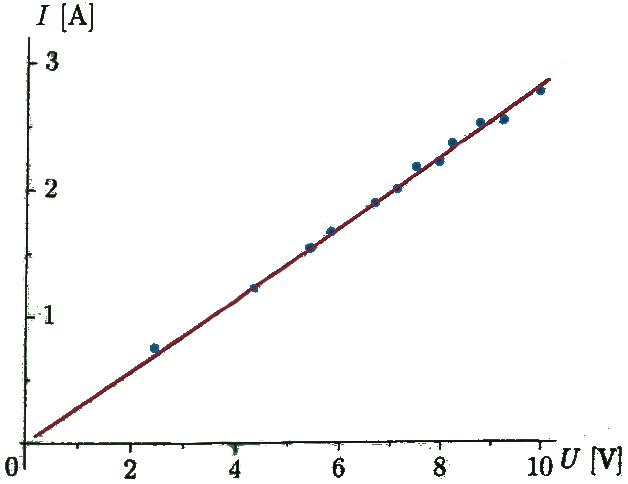
\includegraphics[width=0.8\linewidth]{mai_fig052.png}
  \captionof{figure}{Ověření Ohmová zákona lineární regresí.
  \cite[s.~263]{Musilova2009MA1}
  \label{mai:fig052}}
  \par}
  Pro odpor vychází \(R\doteq\SI{3.52}{\ohm}\). Součet čtverců odchylek přímky se směrnicí \(i/R
  = (1/\num{3.52})\Omega^{-1}\) od souboru bodů grafu je
  \begin{equation*}
    D(R) = \sum_{i=1}^{n}(U_i - R\cdot I_i)^2 \doteq\num{0.01},
  \end{equation*}
  \(\sigma(R) = \sqrt{D(R)/(n-1)}\doteq\sqrt{(\num{0.11}/11)}\doteq\num{0.03}\).  Graf přímky \(U
  = R\cdot I = \num{3.52}\cdot I\) proložené body je na obrázku \ref{mai:fig052}.
\end{mathexam}
      %---------------------------------------------------------------
      
      Popsaný způsob nalezení hodnoty elektrického odporu vodiče v příkladu \ref{mai:exam076} se
      nazývá\textbf{ metodou nejmenších čtverců} (minimalizuje součet čtverců odchylek prokládané
      závislosti od souboru naměřených bodů), v případě použití lineárního modelu, jako tomu bylo u
      Ohmová zákona, pak jde o \textbf{lineární regresi}
      
      Obdobně se postupuje, je-li některá z měřených veličin lineární funkcí veličin jiných s 
      neznámými koeficienty lineární kombinace. Nechť
      \begin{equation*}
        Z = f(X_1, X_2, \ldots, X_K) = A_1X_1 + A_2X_2 + \cdots + A_KX_K.
      \end{equation*}
      Předpokládejme, že veličiny \(X_1, X_2, \ldots, X_K\) a \(Z\) měříme \(n\)-krát a naměříme 
      hodnoty
      \begin{equation*}
        X_j = \lbrace x_{j1}, \ldots x_{jn} \rbrace, \; 1 \leq j \leq K, \; 
        Z = \lbrace z_{1}, \ldots z_{n} \rbrace
      \end{equation*}
      Součet čtverců odchylek teoretické závislosti od naměřených bodů je
      \begin{equation*}
        D(Z) = \sum_{i=1}^{n}\left(z_i - \sum_{j=1}^{K}A_jx_{ji}\right)^2.
      \end{equation*}
      Nutnou podmínkou pro minimum tohoto výrazu jakožto funkce proměnných \(A_x, A_2, \ldots, A_K\)
      je platnost souboru rovnic
      \begin{equation*}
        \pder{D(Z)}{A_p} = 0 \Rightarrow 
        \sum_{i=1}^{n}2\left(z_i - \sum_{j=1}^{K}A_jx_{ji}\right)\cdot x_{pi} = 0
      \end{equation*}
      pro \(1 \leq i \leq n, 1 \leq j \leq K\). Tyto podmínky představují nehomogenní soustavu 
      \(K\) rovnic pro \(K\) neznámých \(( A_1, A_2, \ldots, A_K)\). Rozšířená matice soustavy je
      \begin{strip}
      \begin{equation*}
        \overline{B} = (A\lvert B) = 
          \left(
            \begin{array}{cccc|c}
              \sum_{i=1}^{n}x_{1i}x_{1i} & \sum_{i=1}^{n}x_{1i}x_{2i} & \cdots & 
              \sum_{i=1}^{n}x_{1i}x_{Ki} & \sum_{i=1}^{n}z_{i}x_{1i}                    \\
              \sum_{i=1}^{n}x_{1i}x_{1i} & \sum_{i=1}^{n}x_{2i}x_{2i} & \cdots & 
              \sum_{i=1}^{n}x_{2i}x_{Ki} & \sum_{i=1}^{n}z_{i}x_{2i}                    \\
                        \cdots           & \cdots & \cdots & \cdots   & \cdots          \\
              \sum_{i=1}^{n}x_{Ki}x_{1i} & \sum_{i=1}^{n}x_{Ki}x_{2i} & \cdots & 
              \sum_{i=1}^{n}x_{Ki}x_{Ki} & \sum_{i=1}^{n}z_{i}x_{Ki}                    \\
            \end{array}
          \right),
      \end{equation*}
      \end{strip}
      \begin{equation*}
        \sigma(z) = \sqrt{\dfrac{D(z)}{n - K}}.
      \end{equation*}
      V dalších kapitolách věnovaných lineární algebře se k tomuto problému znovu vrátíme a ukážeme,
      že jej lze elegantně řešit také jako úlohu algebraickou, konkrétně úlohu o ortogonální
      projekci vektorů na podprostory.
      
%} %tikzset
%---------------------------------------------------------------------------------------------------

%-------------------- Theory_of_Derivatives -------------------------------------------------------
  % !TeX spellcheck = cs_CZ
%{\tikzset{external/prefix={tikz/MAI/}}
% \tikzset{external/figure name/.add={ch04_}{}}
%---------------------------------------------------------------------------------------------------
% file: Theory_of_Derivates.tex
%---------------------------------------------------------------------------------------------------
\setchaptertoc
%============== Kapitola: Derivace funkce ==========================================================
\chapter{Derivace funkce}\label{mai:IchapV}
  \section{Hledáme tečny}\label{mai:IchapVsecI}
  \section{Graf funkce snadno a rychle}\label{mai:IchapVsecII}
  \twocolumn[\section{Spokojíme se i s přibližnou hodnotou - diferenciál funkce}\label{mai:IchapVsecIII}]
  \twocolumn[\section{Poznáváme funkci z její derivace - neurčitý integrál}\label{mai:IchapIVsecV}]
  \section{Zpět k logaritmu a exponenciále}\label{mai:IchapVsecV}
  \section{Rozmanité pohyby}\label{mai:IchapVsecVI}
  \section{Od zrychlení k trajektorii}\label{mai:IchapVsecVII}

  \section{Základní věty diferenciálního počtu}\label{mai:IchapVsecVIII}
    \subsection{Věta o největší (nejmenší) hodnotě funkce}
      V tomto článku uvedeme významné věty, zvané souhrně věty o \emph{střední hodnotě 
      diferenciálního počtu}, a dále pak ukázky jejich užití v matematické analýze.  Avšak dříve 
      než budeme tyto věty formulovat, uvedeme jedno důležité tvrzení, které sice bude mít v 
      dalších úvahách tohoto článku pomocnou úlohu, ale v teorii extrémů má i samostatný význam. 
      \cite[s.~186]{Brabec1989} 
      \begin{lemma}\label{MA1:lem_diff02}
        Nechť funkce $f:A\rightarrow\realset$ nabývá na množině $A$ své největší (nejmenší) hodnoty 
        na vnitřním bodě $c$ množiny $A$. Máli funkce $f$ v bodě $c$ derivaci, potom $f'(c)=0$.  
      \end{lemma}
      \begin{proof}
        Nechť např. $f(c)$ je největší hodnota funkce $f$ na množině $A$, takže $f(x)\leq f(c)$ pro
        $\forall x\in A$. Potom pro $x\in A, x<c$, je 
        $$\frac{f(x)-f(c)}{x-c}\geq 0$$
        a tedy
        $$f'_{-}(c)=\lim_{x\rightarrow c^-}\frac{f(x)-f(c)}{x-c}\geq0$$ 
        Dále pro $x\in A, x>c$, je
        $$\frac{f(x)-f(c)}{x-c}\leq 0$$ 
        a proto
        $$f'_{+}(c)=\lim_{x\rightarrow c^+}\frac{f(x)-f(c)}{x-c}\leq0$$
        Platí tedy
        $$f'_{+}(c)\leq f'_{-}(c)\geq f'_{-}(c).$$ 
        Avšak $f'_{+}(c)=f'_{-}(c)= f'(c)$. Odtud plyne $f'(c)=0$. 
      \end{proof}
      
    \subsection{Věty o střední hodnotě}
      \begin{lemma}\label{MA1:lem_diff03}
        \textbf{Rolleova věta}\footnote{Michel Rolle [Mišel Rol] (1652-1719) Francouzský matematik}
        Nechť funkce $f$ má tyto vlastnosti:
          \begin{enumerate}[noitemsep]
            \item je spojitá na uzavřeném intervalu $\langle a,b\rangle$;
            \item má derivaci (vlastní či nevlastní) na otevřeném intervalu $(a,b)$;
            \item platí $f(a)=f(b)$.
          \end{enumerate}
        Potom v otevřeném intervalu $(a,b)$ existuje aspoň jeden bod $\xi$ takový, že $f'(\xi)=0$.   
      \end{lemma}
      \begin{proof}
        Protože je funkce $f$ je na uzavřeném intervalu $\langle a,b\rangle$ spojitá, nabývá v 
        tomto intervalu své největší hodnoty $M$,své nejmenší hodnoty $m$. Přitom ovšem platí:
        \begin{equation}\label{MA1:eq_diff02}
          m\leq f(x) \leq M, \qquad x\in\langle a,b\rangle.
        \end{equation}
        Nyní mohou nastat dva případy: 
        \begin{enumerate}[noitemsep]
          \item funkce $f$ nabývá $M$ i $m$ právě v krajních bodech intervalu $\langle a,b\rangle$. 
                Podle předpokladu 3 věty \ref{MA1:lem_diff03} však potom platí $f(a)=f(b)=m=M$. 
                Vzhledem ke vztahu \ref{MA1:eq_diff02} odtud plyne, že funkce $f$ je konstantní na 
                intervalu $\langle a,b\rangle$ a tedy $f'(x)=0$ dokonce v každém bodě $x\in(a,b)$
          \item Funkce $f$ nabývá apsoň jedné z hodnot $M$, $m$ v některém vnitřním bodě $\xi$ 
                intervalu $\langle a,b\rangle$. Potom podle věty \ref{MA1:lem_diff02} je $f'(\xi)=0$.         
        \end{enumerate}        
      \end{proof}
      \begin{tcnote}
        Rolleova věta sama zaručuje jen existenci aspoň jednoho bodu $\xi\in(a,b)$, ve kterém je fe 
        $f'(\xi)=0$. Neumožňuje však ani určení tohoto bodu (nebo bodů), ani stanovení jejich počtu 
      \end{tcnote}
      
      \begin{tcnote}
        Na obr. \ref{mai:fig027} je ilustrován geometrický význam Rolleovy věty. Graf funkce na 
        tomto obrázku má v bodech $\xi_1$, $\xi_2$, v nichž je $f'(\xi_1)=f'(\xi_2)=0$ tečny 
        rovnoběžné s osou $x$. 
        {\centering
        \captionsetup{type=figure}
        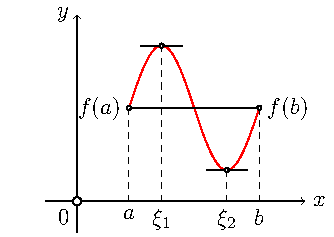
\includegraphics[width=0.7\linewidth]{mai_fig027.pdf}
        \captionof{figure}{K výkladu Rolleovy vět 
        \label{mai:fig027}}
        \par}
      \end{tcnote}
      
      Z Rolleovy věty plyne důležitá věta:
      
      \begin{lemma}\label{MA1:lem_diff04}
        (\textbf{Cauchyova věta}). Nechť funkce $f$ a $g$ mají tyto vlastnosti:
        \begin{enumerate}[noitemsep]
          \item  Jsou spojité na uzavřeném intervalu $\langle a,b\rangle$,
          \item  v každém bodě $x\in(a,b)$ existuje derivace $f'(x)$ (vlastní či nevlastní) a 
                 vlastní derivace $g'(x)$,
          \item  $g'(x)\neq0$ na $(a,b)$
        \end{enumerate}
        Potom v otevřeném intervalu $(a,b)$ existuje aspoň jeden bod $\xi$, pro který platí
        \begin{equation}\label{MA1:eq_diff03}
          \frac{f(b)-f(a)}{g(b)-g(a)} = \frac{f'(\xi)}{g'(\xi)}.
        \end{equation} 
      \end{lemma} 
      
      \begin{proof}
        Poznamenejme především, že z předpokladu 3 $g'(x)\neq0$ pro $x\in(a,b)$ a z předpokladu 
        spojitosti funkce $g$ na uzavřeném intervalu $\langle a,b\rangle$ ihned vyplývá vztah 
        $g(b)- g(a)\neq 0$. Kdyby totiž bylo $g(b)=g(a)$, potom by podle \emph{Rolleovy věty} 
        \ref{MA1:lem_diff03} existoval aspoň jeden bod $\eta\in(a,b)$ takový že $g'(\eta)=0$. To 
        však by byl spor s předpokladem $g'(x)\neq0$ pro každý bod $x\in(a,b)$. Proto má smysl 
        podíl na levé straně rovnosti \ref{MA1:eq_diff03}
        
        K vlastnímu důkazu Cauchyovy věty zavedeme takovou pomocnou funkci $F$, aby splňovala
        podmínky Rolleovy věty. Definujme ji pro $x\in\langle a,b\rangle$ předpisem
        \begin{equation}\label{MA1:eq_diff04}
          F(x)=[f(b)-f(a)]\cdot[g(x)-g(a)]-[f(x)-f(a)]\cdot[g(b)-g(a)].
        \end{equation}
        Snadno ověříme, že tato funkce skutečně splňuje podmínky Rolleovy věty na intervalu $\langle
        a,b\rangle$:
        \begin{itemize}
          \item Je spojitá na intervalu $x\in\langle a,b\rangle$, což je důsledkem spojitosti  
                funkce $f$ a $g$ na intervalu $x\in\langle a,b\rangle$ ,
          \item má derivaci $F'$ na otevřeném intervalu $(a,b)$, což plyne z existence derivace  
                $f'$ a $g'$ funkce $f$ a $g$ na  intervalu $(a,b)$,
          \item $F(a)=F(b)=0$ 
        \end{itemize}
        Platí tedy i závěr Rolleovy věty pro funkci $F$, tj. na intervalu $(a,b)$ existuje aspoň 
        jeden bod $\xi$, pro který $F'(\xi)=0$. Zderivujeme-li funkci $F$, dostaneme (dosadíme-li 
        $x=\xi$): $$F'(\xi)=[f(b)-f(a)]g'(\xi)-f'(\xi)[g(b)-g(a)]=0$$ Odtud již plyne rovnost 
        \ref{MA1:eq_diff03}                  
      \end{proof}
      
      Významným zvláštním případem Cauchyovy věty je další věta, která se častěji používá.
      
      \begin{lemma}\label{MA1:lem_diff05}
        (\textbf{Lagrangeova věta})\footnote{Joseph Louis Lagrange [lagránž] (1736-1813),
        francouzský matematik}. Nechť funkce má tyto vlastnosti:
        \begin{itemize}
          \item Je spojitá na intervalu $\langle a,b\rangle$,
          \item má derivaci (vlastní či nevlastní) na otevřeném intervalu $(a,b)$. 
        \end{itemize} 
        Potom existuje v otevřeném intervalu $(a,b)$ aspoň jeden bod $\xi$, pro který platí 
        \begin{equation}\label{MA1:eq_diff05}
           \frac{f(b) - f(a)}{b - a} = f'(\xi),  
        \end{equation}  
        či-li
        \begin{equation}\label{MA1:eq_diff06}
           f(b) - f(a) = f'(\xi)(b-a),  
        \end{equation}           
      \end{lemma}
      
      \begin{proof}
        Tvrzení této věty je důsledkem tvrzení \emph{Cauchyovy věty}, a to pro případ $g(x)=x$. 
        Protože $g'(x)=1$ dokonce všude, jsou splněny všechny tři podmínky Cauchyovy věty. Proto 
        platí i závěr této věty, z něhož pro náš případ již plyne vzorec \ref{MA1:eq_diff05} a tedy 
        i vzorec \ref{MA1:eq_diff06}.  
      \end{proof}
      
      \begin{tcnote}
        Podobně jako je Lagrangeova věta zvláštním případem věty Cauchyovy, je Rolleova věta
        zvláštním případem Lagrangeovy věty, a to přo případ, že $f(a)=f(b)$.
      \end{tcnote}
      
      \begin{tcnote}
        Lagrangeova věta se často nazývá \emph{větou o přírůstku funkce}, protože vzorcem
        \ref{MA1:eq_diff06} se vyjadřuje \emph{přírůstek funkce}, tj rozdíl $f(b)-f(a)$. Všechny tři
        uvedené věty, tj. věta Rolleova, Cauchyova a Lagrangeova, se v literatuře nazývá souhrně
        \textbf{věty o střední hodnotě diferenciálního počtu}.
      \end{tcnote}
      
      \begin{tcnote}
        Na obr. ** je ilustrován geometrický význam Lagrangeovy věty. Podíl na levé straně rovnosti 
        \ref{MA1:eq_diff05}, tj. číslo $\frac{f(b) - f(a)}{b - a}$ je směrnice sečny $s$, spojující 
        body $A$, $B$ grafu funkce  $f$, které odpovídají krajním bodům intervalu $\langle 
        a,b\rangle$. Podle tvrzení Lagrangeovy věty existuje v otevřeném intervalu $(a,b)$ aspoň 
        jeden bod $\xi$ tak, že tečna grafu funkce $f$ v příslušném jeho bodě je rovnoběžná s 
        přímkou $s$.  
      \end{tcnote}
      
      \begin{tcnote}
        Z Lagrangeovy věty vyplývá toto tvrzení: Nechť funkce $f$ vyhovuje na intervalu $\langle
        a,b\rangle$ podmínkám Lagrangeovy věty a $x_1$, $x_2$ jsou dva libovolné různé body
        intervalu $\langle a,b\rangle$. Potom v otevřeném intervalu s krajnímy body $x_1$, $x_2$
        existuje aspoň jeden bod $\xi$, pro který platí Lagrangeův vzorec:   
        \begin{align}
          f(x_2) - f(x_1)                  &= f'(\xi)(x_2-x_1) \label{MA1:eq_diff07} \\ 
          \frac{f(x_2) - f(x_1)}{x_2-x_1}  &= f'(\xi)          \label{MA1:eq_diff08}      
        \end{align}
        Potom bod $\xi$ lze vyjádřit takto:
        \begin{equation}\label{MA1:eq_diff09}  
          \xi = x_1 + \vartheta(x_2-x_1), \qquad \text{kde }\vartheta\in(0,1). 
        \end{equation}
        Označíme-li $x_2-x_1=h$, můžeme vzorec \ref{MA1:eq_diff07} napsat ve tvaru
        \begin{equation}
          f(x_1+h) - f(x_1)= f'(x_1 + \vartheta h)h, \qquad \text{kde }\vartheta\in(0,1). 
        \end{equation} 
      \end{tcnote}       
          
    \subsection{Některé důsledky Lagrangeovy věty}
      Lagrangeova věta, má některé významné důsledky, které nyní uvedeme \cite[s.~189]{Brabec1989}:
      \begin{lemma}\label{MA1:lem_diff06} 
        Nechť funkce $f$ vyhovuje podmínkám Lagrangeovy věty a navíc nechť $f'(x)=0$ pro všechna 
        $x\in(a,b)$. Potom funkce $f$ je prostá na intervalu $\langle a,b \rangle$. 
      \end{lemma}
      \begin{proof}
        Necť $x_1, x_2$ jsou libovolné dva různé body intervalu $\langle a,b \rangle$. Potom podle 
        Lagrangeova vzorce \ref{MA1:eq_diff04} platí 
        \begin{equation}
          f(x_2) - f(x_1) = f'(\xi)(x_2-x_1) \neq0
        \end{equation}
        neboť $f'(\xi)\neq 0$ dle předpokladu.
      \end{proof}
      
      \begin{lemma}\label{MA1:lem_diff01}
        Funkce $f$ je konstantní na intervalu $(a,b)$, právě když má na tomto intervalu derivaci a
        platí $f'(x) = 0$ pro všechna $x\in(a,b)$. 
      \end{lemma}
      \begin{proof} Tedy
        \begin{itemize}
          \item Je-li funkce $f$ konstantní na intervalu $(a,b)$, pak je $f'(x) = 0$ pro všechna  
                $x\in(a,b)$, jak již víme.
          \item Nechť $f'(x) = 0$ pro všechna $x\in(a,b)$. Dokažme, že pro každé dva body $x_1, 
                x_2  \in(a,b)$, $x_1\neq x_2$, platí $f(x_1) = f(x_2)$. Z existence
                derivace vyplývá spojitost funkce a jsou tedy splněny podmínky Lagrangeovy věty na 
                každém intervalu $\langle x_1, x_2\rangle\subset(a,b)$. Podle vzorce 
                \ref{MA1:eq_diff04} tedy platí $f(x_2)-f(x_1)f'(\xi)(x_2-x_1)$, $\xi\in(x_1,x_2)$. 
                Protože podle předpokladu je $f'(x)=0$ pro $\forall x\in(a,b)$, platí $f(x_1) 
                -f(x_2)=0$, tj. $f(x_1)=f(x_2)$  
        \end{itemize}
      \end{proof}
      
%} % tikzset
%---------------------------------------------------------------------------------------------------
%-------------------- Differential Calculus applications ------------------------------------------
  % !TeX spellcheck = cs_CZ
%{\tikzset{external/prefix={tikz/MAI/}}
% \tikzset{external/figure name/.add={ch05_}{}}
%---------------------------------------------------------------------------------------------------
% file: Differential_Calculus_applications.tex
%---------------------------------------------------------------------------------------------------
\setchaptertoc
\chapter{Aplikace diferenciálního počtu}\label{mai:IchapVI}

%================Kapitola: Analýza průběhu funkce ==================================================
\section{Analýza průběhu funkce}\label{mai:IchapVIsecI}
  Diferenciální počet má rozsáhlou oblast užití. V této kapitole ukážeme použití výsledků
  předchozích kapitol k vyšetřování průběhu funkce a vlastnosti rovinných křivek. Pomocí derivace
  můžeme studovat vlastnosti funkce, které usnadní vyšetřování jejího průběhu. 

  Jednou z důležitých vlastností funkce je její \uv{monotonie}, kterou jsme definovali již v odst.
  \ref{mai:IchapIIIsecIssecIII} kap. \ref{mai:IchapIII}. Proto je při vyšetřování průběhu
  funkce důležité určit množiny (často jsou to intervaly), na nichž je funkce monotónní, jinak
  řečeno, najít \uv{intervaly monotonie funkce} (viz
  \cite[s.~208]{Brabec1989}). 
    \begin{enumerate}[noitemsep]
      \item Zjistíme \textbf{definiční obor funkce}, vyjádříme jej v intervalech a z nich poznáme,
        kde je funkce \textbf{spojitá}. Funkce je spojitá v $(a,b)$ pro každý bod tohoto intervalu,
        když $\abs{f(x)-f(c)}<\varepsilon$, kde $\varepsilon>0$ je libovolně zvolené číslo, a pro
        všechna $x$ z okolí bodu $c$ je $\abs{x-c}<\delta$, kde $\delta>0$ je na $\varepsilon$
        nezávislé.
      \item Určíme, je-li funkce \textbf{lichá} $f(-x)=-f(x)$ nebo \textbf{sudá} $f(-x)=f(x)$. Je-li
        funkce lichá, je souměrná podle středu souměrnosti (obyčejně to bývá počátek souřadnic
        $xy$), je-li sudá, je souměrná podle osy $y$.
      \item Určíme \emph{průsečíky křivky s osami pravoúhlých souřadnic}. Body, ve kte\-rých křivka
        protíná osu $x$ spolu s body, ve kte\-rých není křivka spojitá, rozlišují intervaly, v nichž
        je graf křivky nad osou $x$ od intervalů, ve kterých je graf křivky pod osou $x$.
      \item V krajních bodech definičních intervalů, ve kterých je funkce spojitá, stano\-víme
      \emph{limity funkce} a dále $$\lim_{x \to \pm \infty}f(x).$$
      \item Vypočítáme $f'(x)$ a $f''(x)$, abychom zjistily, kde je funkce \emph{rostoucí}     
        $f'(x)>0$, \emph{klesající} $f'(x)<0$ a kde jsou \emph{lokální extrémy}. Dostaneme-li
        dosazením kořenů rovnice $f'(x)=0$ do $f''(x)$ hodnotu $f''(x)>0$, má funkce lokální
        minimum, při $f''(x)<0$ má funkce lokální maximum. V intervalech, kde $f''(x)>0$, je křivka
        \textbf{konvexní (vypuklá)}, kde $f''(x)<0$, je křivka \textbf{konkávní (vydutá)}. Body, v
        nichž $f''(x)$ mění znaménko, jsou \textbf{inflexní body}. Najdeme je tak, že stanovíme
        hodnoty $x$, pro které je $f''(x)=0$ nebo neexistuje. Číslo $c$ je inflexní bod, když
        existuje takové okolí bodu $c$, že pro $x>c$ je oblouk křivky konvexní a pro $x<c$ konkávní.
        Je nutné si uvědomit, že když má $f'(x)$ konečnou derivaci, je inflexní bod $c$ taky nulovým
        bodem druhé derivace čili kořenem rovnice $f''(x)=0$. Obrácená věta neplatí, tj. z
        $f''(x)=0$ nevyplývá, že v bodě $c$ má $f'(x)$ extrém a že bod $c$ je inflexním bodem.
      \item \textbf{Asymptota} je tečna křivky $f(x)$, jejíž bod dotyku je v nekonečnu. Platí-li  
        $$\lim_{x \to a}f(x) =  \pm\infty,$$ je přímka $x=a$ její asymptotou. Jinak asymptoty mají
        rovnici $y=kx+q$, kde $x$ a $y$ jsou souřadnice bodů na asymptotách. Existují-li konečné
        limity $$\lim_{x \to \pm\infty}\frac{f(x)}{x}=k$$  a $$\lim_{x \to \pm\infty}[f(x)-kx] =q$$
        pak je asymptotou přímka $y=kx+q$. Můžeme-li rovnici křivky rozložit (tj. rozložit její
        pravou stranu, oby\-čejně dělením čitatele jmenovatelem, má-li tvar zlomku) na dvě části, z
        nichž jedna má tvar $kx+q$ a druhá zbytek $\varphi(x)$, tj. $f(x)=kx+q+\varphi(x)$ a
        $\varphi(x)_{x\rightarrow \pm\infty}\rightarrow 0$, je přímka $y=kx+q$ asymptotou.
      \item Zpřesnění grafu křivky provedeme sestavením tabulky souřadnic dalších bodů křivky, tj.
        ke zvoleným hodnotám $x$ (z definičního oboru funkce) vypočítáme hodnoty $y$. Do dalších
        řádků tabulky zapíšeme hodnoty  $f'(x)$ a $f''(x)$, ve kterých intervalech je funkce
        \emph{rostoucí}, ve kterých \emph{klesá}, kde je \emph{vypuklá}, kde je \emph{dutá}, kde
        jsou \emph{lokální extrémy}, \emph{inflexní body} apod., případně sestavíme dílčí tabulky
        pro jednotlivé \emph{charakteristické vlastnosti} vyšetřované funkce.
    \end{enumerate}
    %-------------------- EXAM001 --------------------------------------
    % !TeX spellcheck = cs_CZ
\begin{mathexam}{Vyšetřete průběh funkce \(f(x):y=\frac{1+x^2}{1-x^2}\)}{exam003}
  \begin{enumerate}[noitemsep]
    \item Definiční obor $D_f=\realset-\{±1\}=(-\infty,-1)\cup(-1,1)\cup(1,+\infty)$
    \item Funkce je sudá $$f(-x)=f(x): \frac{1+x^2}{1-x^2}=\frac{1+(-x)^2}{1-(-x)^2}.$$ Funkce není
        periodická.
    \item Stanovíme funkční hodnoty v krajních bodech definičního obor $1, -1$ a v nevlastních
        bodech $-\infty,+\infty$.Protože je funkce \textbf{sudá}, omezíme se jen na vyšetřování
        nezáporné části. Nejprve vlastnosti funkce v okolí bodu $1$. Ten nepatří do $D_f$ a proto
        určíme limity funkce v pravém a levém okolí tohoto bodu. $$\lim_{x\to
        1_{-}}=\frac{1+x^2}{1-x^2}.$$ Pro výpočet limity použijeme substituci $y=1-x^2$: 
        $$\lim_{y\to0+}\frac{2-y}{y}=+\infty$$ \footnote{$\lim_{x\to0_+}\frac{1}{x}=\infty$} proto
        
        $$\lim_{x\to1_{-}}\frac{1+x^2}{1-x^2}=+\infty.$$ Obdobně dojdeme k
        $$\lim_{x\to1_+}\frac{1+x^2}{1-x^2}=-\infty.$$ A konečně v nevlastních bodech $±\infty$ je
        limita $$\lim_{x\to±\infty}\frac{1+x^2}{1-x^2} = \lim_{x\to\pm\infty}\frac{1}{1-x^2} +
        \lim_{x\to\pm\infty}\frac{x^2}{1-x^2}=0-1=-1.$$ Výpočtem limit jsme zároveň určili dva
        absolutní (globální) extrémy a jeden lokální:
        \begin{itemize}
          \item v intervalu $(-1,1)$ má funkce maximum $\infty$ a minimum $1$,
          \item v intervalech $(-1,1)\cup(1,+\infty)$ má funkce minimum $-\infty$ a maximum $-1$.
        \end{itemize}
    \item Nyní vyšetříme zda, případně kolik a jaké, má funkce $f(x)$ průsečíky s osami souřadnic. S
        osou $x$ nemá funkce žádné průsečíky, protože pro $y=0$ není definována
        $H_f=\realset-\{-1,1\rangle$. Pro $x=0$ je $y=\frac{1+0^2}{1-0^2}=1$, proto má $f(x)$ právě
        jeden průsečík s osou $y$ a to $[0,1]$.
    \item Zatím jsme zjistili, že naše funkce není definována v bodech $1$ a $-1$ a proto není
        spojitá v  $\realset$. Nevíme však, jaký je její průběh v jednotlivých intervalech
        definičního oboru.  Abychom získali názornější představu o průběhu funkce, zjistíme má-li
        derivaci.
        \begin{align*}
          y' &= \frac{(1+x^2)'(1-x^2 )-(1+x^2)(1-x^2 )'}{(1-x^2)^2} \\
          y' &= \frac{2x(1-x^2 )-(1+x^2 )(-2x)}{(1-x^2 )^2}         \\
          y' &= \frac{4x}{(1-x^2 )^2}
        \end{align*}
        Protože má vlastní derivaci\footnote{$f(x)$ je spojitá v intervalech $(-\infty,-1),
        (-1,1),(1,\infty)$  věta s spojité funkci}, můžeme určit její vlastnosti v intervalech
        $\langle0,1)$ a $(1,\infty)$. V těchto intervalech je $y'>0$ a proto jde o funkci ryze
        monotónní, rostoucí \footnote{Plyne z věty o postačujících podmínkách ryzí monotónnosti
        funkce na intervalu} v daných intervalech \footnote{V intervalech
        $(-\infty,-1),(-1,0\rangle$ je funkce klesající.}. Výpočtem zjistíme druhou derivaci funkce.
        Ta nám pomůže určit další extrém v intervalu $\langle0,1)$ a zároveň vyšetřit
        \textbf{konkávnost} a \textbf{konvexnost}.
        \begin{align*}
          y'' &= \frac{(4x)' (1-x^2 )^2-(4x)(1-2x^2+x^4 )'}{(1-x^2 )^4}  \\
          y'' &= \frac{4(1-2x^2+x^4 )-4x(-4x+4x^3 )}{(1-x^2 )^4}         \\
          y'' &= \frac{4(1-x^2 )(3x^2+1)}{(1-x^2 )^4}                    \\
          y'' &= \frac{4(3x^2+1)}{(1-x^2 )^3}
        \end{align*}
        Abychom mohli určit lokální extrém funkce $f(x)$ v intervalu $\langle0,1)$, pomocí druhé
        derivace, musíme najít kořeny rovnice $f' (x)=0$. V našem případě
        $$y'=\frac{4x}{(1-x^2)^2}\Rightarrow\frac{4x}{(1-x^2)^2}=0\rightarrow x_0=0,$$ tento kořen
        \footnote{stacionární bod}  pak dosadíme do druhé derivace, tj. 
        $$y''(0)=\frac{4(3\cdot0^2+1)}{(1-0^2 )^3}=4,$$ protože je $f''(x)>0$, má v bodě $x_0$
        lokální minimum. Můžeme rovněž konstatovat, že funkce nemá inflexní body \footnote{Pro
        existenci inflexního bodu je nutné splnění jedné z podmínek a to buď $f''(x_0)=0$, nebo
        $f''(x_0)$ neexistuje.}. Konkávnost a konvexnost funkce v intervalech $\langle0,1)$ a
        $(1,\infty)$ vyšetříme pomocí vlastností druhé derivace funkce. Tedy
        \begin{itemize}
          \item $\langle0,1): y''=\frac{4(3x^2+1)}{(1-x^2 )^3} >0 \Rightarrow$ funkce je v tomto
                intervalu \textbf{konvexní},
          \item $(1,\infty): y''=\frac{4(3x^2+1)}{(1-x^2 )^3} <0 \Rightarrow$ funkce je v tomto
                intervalu \textbf{konkáv\-ní}.
        \end{itemize}
    \item Z předchozích výpočtů plyne, že křivka má asymptoty $y=-1,x=\pm1$.
  \end{enumerate}
  {\centering \captionsetup{type=figure}          % %\ref{MAI:fig_028}
    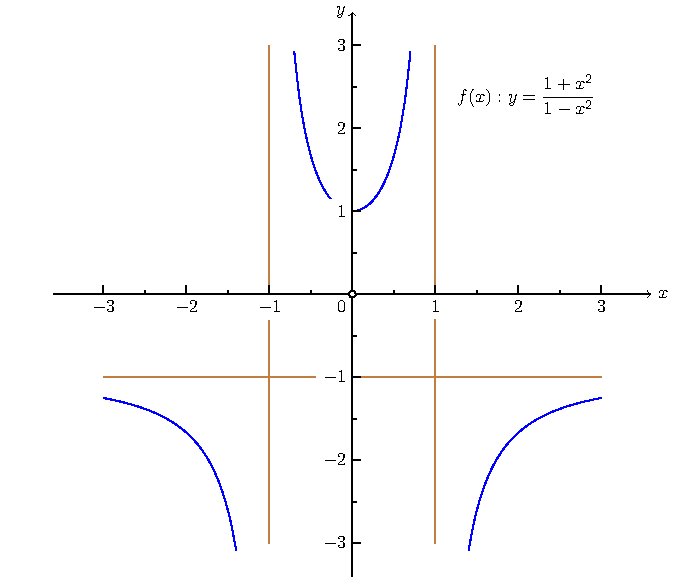
\includegraphics[width=1\linewidth]{mai_fig028.pdf}
    \captionof{figure}{Graf funkce $f(x):y=\dfrac{1+x^2}{1-x^2}$}
    \label{MAI:fig_028}
  \par}
\end{mathexam}  
    %-------------------------------------------------------------------

%================Kapitola: Aplikace diferenciálního počtu =========================================
\section{Fyzikální a jiné aplikace derivace}\label{mai:IchapVIsecII}
    V předcházející kapitole \ref{mai:IchapVIsecI} jsou uvedeny jednoduché příklady na užití první a
    druhé derivace. V této kapitole jsou soustředěny slovní úlohy na maxima a minima z různých
    oborů.
    %--------------------------------------------------------------
    % !TeX spellcheck = cs_CZ
\begin{mathexam}{Je dán trojúhelník s vrcholy \(A[0, 0]\), \(B[4, 0]\), \(C[1, 3]\). Mezi všemi
  obdélníky vepsanými danému trojúhelníku, se stranou („základnou“) \(z\) ve straně \(c\) (označení
  viz obr. \ref{mai:fig062}), máme najít ten, který má maximální obsah.}{exam092}

  {\centering
    \captionsetup{type=figure}
    \includegraphics[width=1\linewidth]{mai_fig062.png} 
    \captionof{figure}{K příkladu \ref{mai:exam092}. Kredit: \cite[s.~46]{rektorys2011}}
    \label{mai:fig062}
  \par}
  
  Napišme nejprve rovnice stran \(a\), \(b\). Strana \(b\) (přesněji: přímka obsahující stranu
  \(b\)) má zřejmě rovnici
  \begin{equation*}
    y = 3x
  \end{equation*}
  Přímka, v níž leží strana \(a\), má směrnici
  \begin{equation*}
    k = \dfrac{3-0}{1-4} = -1,
  \end{equation*}
  a tedy podle rovnice \(y-y_0 = k(x-x_0)\) dostáváme 
  \begin{equation*}
    y - 0 = -1\cdot(x - 4) \quad\Rightarrow\quad y = -x + 4.  
  \end{equation*}
  Pro obsah \(S\) vepsaného obdélníka platí podle označení v obr. \ref{mai:fig062} 
  \begin{equation*}
    S = zv.
  \end{equation*}
  Za proměnnou zde bude výhodné volit „výšku“ \(v\). „Základnu“ \(z\) pak vypočteme (viz obr.
  \ref{mai:fig062}) jako rozdíl
  \begin{equation}\label{mai:eq087}
    z = x_2 - x_1,
  \end{equation}
  kde \(x_1\), resp. \(x_2\) je souřadnice \(x\) průsečíku přímky \(y = v\) (přímka \(p\) na obr.
  \ref{mai:fig062}) se stranou \(b\), resp. \(a\). Rovnice těchto stran jsou dány vztahy \(y = 3x\)
  a \(y = -x + 4\). Dosadíme-li podle \(y = v\rightarrow\)  \(v\) za \(y\) do těchto rovnic,
  dostaneme právě \(x_1\) a \(x_2\). Bude
  \begin{equation*}
    v = 3x_1, \qquad v = -x_2 + 4,
  \end{equation*}
  odkud (při zvoleném \(v\)) plyne
  \begin{equation*}
    x_1 = \dfrac{v}{3}, \qquad  x_2 = 4 - v 
  \end{equation*}
  a podle \ref{mai:eq087}
  \begin{equation*}
    z = x_2 - x_1 =  4 - \dfrac{4}{3}v
  \end{equation*}
  a konečně pro obsah vepsaného obdélníku dostáváme jednoduchou rovnici
  \begin{equation}\label{mai:eq088}
    S = zv = \left(4 - \dfrac{4}{3}v\right)v = 4v - \dfrac{4}{3}v^2.
  \end{equation} 
  Tím je obsah \(S\) obdélníka daný jako funkce zvolené výšky \(v\). Zvolíme-li například \(v=1\),
  bude obsah \(S\) obdélníka z obr. \ref{mai:fig062} roven číslu \(4\cdot1 - \frac{4}{3}\cdot1^2\). 
  
  Budeme hledat (absolutní) maximum funkce (\ref{mai:eq088}) na intervalu \(\langle0,3\rangle\)
  (neboť nemůžeme zvolit \(v\) větší než 3). Ale pro \(v=0\) a \(v=3\) je \(S=0\) a všude jinde je
  \(S > 0\), takže budeme hledat lokální maximum funkce (\ref{mai:eq088}) na otevřeném intervalu
  \((0,3)\). Derivováním (\ref{mai:eq088}) podle proměnné \(v\) však máme
  \begin{equation*}
    S' = 4 - \dfrac{8}{3}v, \qquad S'' = -\dfrac{8}{3}.
  \end{equation*}
  Položíme-li nyní pravou stranu rovnu nule, dostaneme 
  \begin{equation*}
    4 - \dfrac{8}{3}v = 0 \quad\Rightarrow\quad v = \dfrac{12}{8} = \dfrac{3}{2}.
  \end{equation*}
  Přitom podle druhé derivace obsahu je všude, a tedy i v bodě \(\frac{3}{2}\), je
  \(S''=-\frac{8}{3}<0\) takže v bodě \(v = \frac{2}{3}\) je ostré lokální maximum. Zároveň pro
  \(v=\frac{3}{2}\) bude
  \begin{equation*}
    z = 4 - \dfrac{4}{3}\cdot\dfrac{3}{2} = 2.
  \end{equation*}
  Hledaný obdélník maximálního obsahu bude mít rozměry: \(z = 2\), \(v = \frac{3}{2}\), a tedy obsah
  \(S = 3\).    
\end{mathexam}
    %--------------------------------------------------------------

    %--------------------------------------------------------------
    % !TeX spellcheck = cs_CZ
\begin{mathexam}{Z břevna kruhového průřezu s poloměrem \(r = \protect\SI{20}{\protect\cm}\) máme
  vytesat trám, který bude mít průřez ve tvaru obdélníka se stranami \(z\) a \(v\) („základnou“ a
  „výškou“). Jak máme volit \(z\) a \(v\), aby trám měl maximální nosnost, víme-li, že jeho nosnost
  je úměrná první mocnibibeně \(z\) a druhé mocnině \(v\)?}{exam091}
   
  {\centering
    \captionsetup{type=figure}
    \includegraphics[width=1\linewidth]{mai_fig061.png} 
    \captionof{figure}{K příkladu \ref{mai:exam091}. Kredit: \cite[s.~47]{rektorys2011}}
    \label{mai:fig061}
  \par}
  
  Matematická formulace: Jaké rozměry má mít obdélník vepsaný do kružnice s poIoměrem \SI{20}{\cm},
  má-li být součin základny \(z\) a druhé mocniny výšky v maximální,
  \begin{equation*}
    y = z\cdot v^2 = ?
  \end{equation*}
  Zvolme za proměnnou z. Podle Pythagorovy věty platí (viz \ref{mai:fig061})
  \begin{equation*}
      r^2 = \left(\dfrac{z}{2}\right)^2 + \left(\dfrac{v}{2}\right)^2,
  \end{equation*}
  odkud 
  \begin{equation*}
      v^2 = 4r^2 - z^2.
  \end{equation*}
  Máme tedy najít maximum funkce
  \begin{equation}\label{mai:eq086}
      y = zv^2 = z(4r^2 - z^2) = 4r^2z - z^3,
  \end{equation}
  a to na intervalu \((0,40)\), neboť \(z\) nemůže být větší než \(2r = 40\). Ale funkce
  (\ref{mai:eq086}) je na tomto intervalu nezáporná a pro \(z = 0\) a \(z = 40\) je rovna nule
  (neboť pak \(4r^2 - z^2 = 0\). Hledáme tedy lokální maximum funkce (\ref{mai:eq086}) v otevřeném
  intervalu \(0,40)\). 

  Funkce (\ref{mai:eq086}) má všude první a druhou derivaci,
  \begin{equation*}
      y' = 4r^2 - 3z^2, \qquad\qquad y'' = -6z.
  \end{equation*}
  Může tedy předně nabývat v intervalu \((0, 40)\) lokálního extrému jen tam, kde je \(y'=0\), tj.
  kde
  \begin{equation*}
      4r^2 - 3z^2 = 0.
  \end{equation*}
  Odtud plyne, neboť má být \(z > 0\), že
  \begin{equation*}
      z = \sqrt{\dfrac{4r^2}{3}} = \dfrac{2}{\sqrt{3}}r = \dfrac{2\sqrt{3}}{3}r = 
          \dfrac{2\sqrt{3}}{3}20 \simeq \num{23.1}.
  \end{equation*}
  Pro \(v\) pak \(z\) dostaneme
  \begin{equation*}
      v = \sqrt{4r^2 - \dfrac{4}{3}r^2} = \sqrt{\frac{8}{3}\cdot20^2}\simeq\num{32.6}
  \end{equation*}
  V bodě \(z = \num{23.1}\) bude mít funkce (\ref{mai:eq086}) skutečně lokální maximum, a to ostré,
  neboť druhá derivace je v tomto bodě záporná.
\end{mathexam}
    %--------------------------------------------------------------

    %--------------------------------------------------------------
    % !TeX spellcheck = cs_CZ 
\begin{mathexam}{Světelný zdroj \(B\) (např. pouliční svítilna) má vzdálenost \qty{36}{\m} od
  světelného zdroje \(A\). Zdroj \(B\) má osmkrát větší intenzitu než zdroj \(A\). Který bod na
  spojnici obou zdrojů bude nejméně osvětlený? (Přitom intenzita osvětlení světelným zdrojem je
  přímo úměrná intenzitě zdroje a klesá s druhou mocninou vzdálenosti od uvažovaného
  zdroje.)}{exam093} 
  
  {\centering
    \captionsetup{type=figure}
    \luafigure[1]{mai_fig063.png} 
    \captionof{figure}{K příkladu \ref{mai:exam093}. Kredit: \cite[s.~48]{rektorys2011}}
    \label{mai:fig063}
  \par}      

  Matematická formulace: Označme \(a\) intenzitu zdroje \(A\). Pak intenzita zdrojo \(8\) je \(8a\).
  Označme dále \(x\) vzdálenost bodu \(P\) na spojnici bodů \(A\) a \(B\) meřenou od zdroje \(A\).
  Pak intenzita osvětlení v bodě \(P\) od zdroje \(A\) bude úměrná číslu \(\frac{a}{x^2}\) zdroje B
  číslu \(\frac{8a}{(36 - x)^2}\) (se stejnou konstantou úměrnosti). Máme tedy najít v intervalu
  \((0,36)\) takové \(x\), pro které bude součet obou intenzit minimalni, a tj.
  \begin{equation}\label{mai:eq089}
    y = \dfrac{a}{x^2} + \dfrac{8a}{(36 - x)^2} = \text{min}
  \end{equation}
  Ale funkce \ref{mai:eq089} má všude v otevřeném intervalu  \((0,36)\) první a druhou derivaci.
  Nastává chvíle si procvičit derivování podílu:
  \begin{gather*}
    \begin{align*} 
      \left(\dfrac{a}{x^2}\right)'          
        &= (ax^{-2})' = -\dfrac{2a}{x^3},   \\ 
      \left( \dfrac{8a}{(36 - x)^2}\right)' 
        &= \dfrac{(8a)'\cdot(36 - x)^2 - (8a)\cdot(36^2 - 72x + x^2)'}{(36 - x)^4} \\
        &= \dfrac{-8a(-72 + 2x)}{(36 - x)^4} 
         = +\dfrac{8a\cdot2\cdot\cancel{(36 - x)}}{(36 - x)^{\cancel{4}3}}
         =  \dfrac{16a}{(36 - x)^3}
    \end{align*}
  \end{gather*}
  (neboť \(8a = \text{konst}\), takže \((8a)' = 0\); k derivování funkce \(8a/(36 - x)^2\) jsme také
  mohli místo věty o derivování podílu použít větu o derivování složených funkcí a psát
  \begin{equation*}
    \dfrac{8a}{(36 - x)^2} = \dfrac{8a}{z}, \quad\text{kde}\quad z = 36 - x
  \end{equation*}  
  Tedy 
  \begin{align*}
    y'  &= -\dfrac{2a}{x^3} + \dfrac{16a}{(36 - x)^3} \\
    y'' &=  \dfrac{6a}{x^4} + \dfrac{48a}{(36 - x)^4}. 
  \end{align*}
  Jak víme, v bodě lokálního minima bude \(y' = 0\)
  \begin{equation}\label{mai:eq090}
    -\dfrac{2a}{x^3} + \dfrac{16a}{(36 - x)^3} = 0.
  \end{equation}
  Rovnici můžeme řešit tak, že zlomky na levé straně dáme na společného jmenovatele. (Zkuste to,
  nebude to hezká rovnice!) Ale má být \(x > 0\), \(36 - x > 0\), takže (\ref{mai:eq090}) můžeme
  zapsat ve tvaru
  \begin{align*}
    \dfrac{(36 - x)^3}{x^3} &= -\dfrac{16a}{2a} = 8 \qquad\text{takže}      \\
    \dfrac{36 - x}{x}       &= \sqrt[3]{8} \Rightarrow 36 - x = 2x.
  \end{align*}
  Zároveň \(y''>0\), takže v bodě \(x=12\) bude ostré lokální minimum. Nejméně osvětlený bod bude
  tedy ve vzdálenosti \qty{12}{\m} od zdroje \(A\).

  {\centering
  \captionsetup{type=figure}
  \luafigure[1]{mai_fig064.pdf} 
  \captionof{figure}{K příkladu \ref{mai:exam093}.}
  \label{mai:fig064}
  \par}   
\end{mathexam}
    %--------------------------------------------------------------

%} %tikzset
%---------------------------------------------------------------------------------------------------
%--------------------Primitive Functions ----------------------------------------------------------
  % % !TeX spellcheck = cs_CZ
%---------------------------------------------------------------------------------------------------
% file: mai1ch07.tex
%---------------------------------------------------------------------------------------------------
%============================ Primitivní funkce ====================================================
\setchaptertoc
\chapter{Poznáváme funkci z její derivace - neurčitý integrál}
  %----------------------------Neurčitý integrál----------------------------------------------------
  \section{Motivace}
    Problém \emph{neurčitého integrálu}, neboli \textbf{primitivní funkce}, lze vyložit velmi 
    jednoduše: Máme podezření, že zadaná funkce \(f(x)\) vznikla derivováním jisté, zatím neznámé, 
    funkce \(F(x)\). Dokážeme ji najít? 
  
    K danému problému můžeme přistupovat také fyzikálně: Zavedením pojmu derivace funkce jsme 
    motivovali důležitým požadavkem definovat okamžitou rychlost pohybu bodu po přímce. Existuje 
    přirozeně i požadavek opačný, tj. nalézt zákon dráhy pohybu bodu po přímce, je-li dána jeho 
    okamžitá rychlost jako funkce času \cite[s.~253]{Brabec1989}. Vše si ukážeme na následujícím 
    příkladu:      
    %-------------------------------------
    % !TeX spellcheck = cs_CZ
%====================== Sbírka řešených příkladů ==================================================
\begin{mathexam}{Je dána okamžitá rychlost \(v\) pohybu bodu po přímce (ose) \(x\) rovnicí \(v(t) =
  2t + 1\), \(t\in\langle -\infty,+\infty \rangle\). Najděte zákon dráhy pohybu, je-li známo, že v
  čase \(t = 0\) měl bod polohu \(x = x_0\) \cite[p.~253]{Brabec1989}.}{exam117}

  Označíme-li \(x(t)\) polohu bodu v okamžiku \(t\), pak \(v(t) = \frac{dx}{dt}\). Hledáme tedy
  funkci \(x = x(t)\), pro níž platí \[\frac{dx}{dt} = 2t + 1 \qquad x(0) = x_0.\] Je ihned patrné,
  že první podmínce vyhovuje nekonečně mnoho funkcí
  \begin{equation}\label{MA:int_ex_09}
    x(t) = t^2 + t + c, 
  \end{equation}
  kde \(c\) je libovolná konstanta. Funkce, která splňuje i druhou podmínku (říkáme ji též počáteční
  podmínka), najdeme z rovnice \ref{MA:int_ex_09} dosazením dané podmínky \(t = 0\), \(x = x_0\).
  Dostaneme \(x_0 = c\). Dosazením do \ref{MA:int_ex_09} za \(c\) plyne hledaný zákon dráhy \(x(t) =
  t^2+t+x_0\).                 

  Jednoduchou zkouškou se přesvědčíme, že tato funkce splňuje obě dané podmínky a zároveň vidíme, že
  hledaná primitivní funkce daných vlastností je jediná.
\end{mathexam}
    %-------------------------------------
    Každé takové funkci, jejíž derivací je daná funkce, budeme říkat \emph{primitivní funkce} k 
    dané funkci. Na uvedeném příkladě je patrné, že k dané funkci může existovat nekonečně mnoho 
    primitivních funkcí. Množinu všech primitivních funkcí se často nazývá \textbf{neurčitým 
    integrálem}. Po tomto názorném uvedení do problému přejděme k přesné formulaci základních pojmů.
    
  \section{Definice primitivní funkce}  
    \begin{mdframed}[style=mdmathdef] 
      \begin{definition}\label{mai:def002}
        Funkci \(F(x): J\rightarrow \realset\), kde \(J\subset \realset\) je interval, nazveme
        \textbf{primitivní} funkcí k funkci \(f(x)\) na intervalu \(J\) právě když, pro všechna
        \(x\in J\) je \(F'(x) = f(x)\). 
        
        V případě uzavřeného intervalu \(J=[a,b]\) požadujeme ještě, aby obě jednostranné derivace
        splňovali \(F_+'(a)=f(a)\) a \(F_-'(b)=f(b)\). 
        
        Množina všech primitivních funkcí k funkci \(f(x)\) na \(J\) se nazývá \textbf{neurčitý
        integrál} z funkce \(f(x)\) a značí se \(\int f(x)\dd{x}\). Tedy
        \begin{gather}\label{mai:eq101}
          \int f(x)\dd{x} = \{F(x): \text{\(F(x)\) je primitivní funkcí k \(f(x)\) na \(J\)}\}
        \end{gather}
      \end{definition}
    \end{mdframed}
    %-------------------------------------
    % !TeX spellcheck = cs_CZ
%====================== Sbírka řešených příkladů ==================================================
\begin{mdframed}[style=mdexam]
  \begin{example}\label{mai:exam118}
    K funkci $\sin x$ je primitivní funkcí na libovolném intervalu $J\subset(-\infty,+\infty)$ 
    funkce $-\cos x$, protože $(-\cos x)' = \sin x$. Ale též funkce $3-\cos x$ je primitivní 
    funkcí k funkci $\sin x$, protože $(3 - \cos x)' = \sin x$ pro všechna $x\in(-\infty, 
    \infty)$.
  \end{example}
\end{mdframed}
    %-------------------------------------
    
    Z uvedených příkladů je vidět, že rozdíl dvou primitivních funkcí k téže funkci je konstanta. To
    není náhoda, jak potvrzuje následující věta:

    \begin{mdframed}[style=mdmathlemma] 
      \begin{lemma}\label{mai:lemma008}(Věta o rozdílu dvou primitivních funkcí)
        \begin{enumerate}[noitemsep]
          \item Je-li funkce $F$ primitivní funkcí k funkci \(f\) na intervalu \(J\) a \(c\) reálná  
                konstanta, pak i funkce $G = F + c$ je primitivní funkcí k funkci \(f\) na intervalu 
                \(J\).
          \item Jsou-li funkce $F$ a $G$ primitivní funkce k funkci \(f\) na intervalu \(J\), pak 
          funkce
                $F-G$ je na intervalu \(J\) konstantní.
        \end{enumerate} 
        \begin{proof}
          Tvrzení a) plyne z definice protože $G'(x) = [F(x) + c] = F'(x) = f(x)$ pro všechna $x\in
          J$. Tvrzení b) je důsledkem věty \ref{MA1:lem_diff01}.
        \end{proof}
      \end{lemma}
    \end{mdframed}

    \subsection{Poznámky k definici}  
      Z definice \ref{mai:def002} vyplývá, že primitivní funkce je spojitou funkcí, neboť má
      derivaci a věta \ref{mai:lemma008} nám říká, že pokud k dané funkci existuje funkce
      primitivní, existuje jich nekonečně mnoho. Je-li např. \(F\) primitivn9 funkce k funkci \(f\)
      na intervalu \(J\), pak množina všech primitivních funkcí je množina \(\{F + c;
      c\in\realset\}\). Tuto množinu označujeme symbolem \(\int f(x)\dd{x}\) a čteme \uv{integrál
      \(f(x)\dd{x})\)} Symbolu \(\int f(x)\dd{x}\) říkáme \textbf{neurčitý integrál}. Zpravidla
      píšeme
      \begin{mdframed}[style=mdmathlemma]  
        \begin{equation}\label{mai:eq102}
          \int f(x)\dd{x} = F(x) + c
        \end{equation}
      \end{mdframed}
      nebo jen \(\int f(x)\dd{x} = F(x)\) (tj. aditivní konstantu vynecháváme) a máme tím na mysli
      že \(F(x) \in \int f(x)\dd{x}\). Rovnost \ref{mai:eq102} je tedy rovnost mezi množinami,
      nikoliv rovnost funkcí. 
    
    \subsection{Některé vlastnosti integrálů}  
      Platnost několika následujících vztahů lze prověřit přímo užitím definic derivace a neurčitého
      integrálu. Tyto vztahy jsou při výpočtech často používány. Nejprve však uvedeme základní
      pravidla pro primitivní funkce, která plynou z pravidel pro derivování:
      \begin{subequations}
        \begin{flalign}
          \int\dd{f(x)} &= f(x) + c,                                          &\label{mai:eq134} \\
          \dxd\left[\int f(x)\dd{x}\right] &= f(x)\dd{x},                     &\label{mai:eq135} \\
          \int[f(x)\pm g(x)]\dd{x}&= \int f(x)\dd{x} + \int g(x)\dd{x},       &\label{mai:eq103} \\
          \int kf(x)\dd{x}      &=k\int f(x)\dd{x},\quad\text{\(k=\) konst.}, &\label{mai:eq104} \\
          \left[\int f(x)\dd{x}\right]' &= f(x),                              &\label{mai:eq136}
        \end{flalign}
      \end{subequations}
  
  \section{Tabulka neurčitých integrálů}\label{MA:chap_tabINT}
    Jak ale primitivní funkce hledat? V jednoduchých příkladech poslouží tabulka derivací, již čteme
    „zprava doleva“. (Je dobré si ji uložit do paměti.) Tabulka však pokryje jen velmi málo případů,
    pouze elementární funkce. Je tedy třeba najít metody, jak při hledání primitivních funkcí
    postupovat.

    Uveďme nyní některé základní integrály. Poznamenejme, že touto tabulkou nejsou zdaleka vyčerpány
    všechny funkce, ke kterým umíme primitivní funkce najít. Existují celé knihy obsahující tabulky
    integrálů a programy výrazně ulehčující hledání primitivních funkcí. Literatura:
    \cite{Rektorys1963}, \cite{Brabec1989}, \cite{diblik2002}. 

    Pokud není nic uvedeno, platí vzorce pro všechna \(x\) a pro všechny hodnoty uvedených konstant.
    Místo platí pro \(x\) z intervalu \((-\infty,0),(0,+\infty)\) píšeme stručně \(x\neq0\) apod.
    Obory platnosti uvádíme jen tam, kde nejsou evidentní.  

    \begin{flalign}
      \midrule
      & \int 0\dd{x} = c                                        &      \label{mai:eq105}     \\
      & \int a\dd{x} = ax+c                                     &      \label{mai:eq106}     \\
      & \int x^n\dd{x} = \frac{x^{n+1}}{n+1}+c,                 &      \label{mai:eq107}     \\              
        \shortintertext{\hspace{2em} kde \(\begin{cases}
          \forall x\in\realset,\,n\in\naturalset, n>0,         \\
          \forall x\in\realset-\{0\},\,n\in\naturalset, n<-1,  \\
          \forall x>0,\,n\in\realset\,\,n\neq-1
        \end{cases}\)}                                          
      & \int\frac{1}{x}\dd{x} = 
            \ln\abs{x}+c \hspace{1ex}\forall x\neq0            &       \label{mai:eq108}    \\
      & \int e^x \dd{x}       = e^x+c                          &       \label{mai:eq109}    \\
      & \int\ln x\dd{x}       = 
          x\ln x - x + c \hspace{1ex}\forall x>0               &       \label{mai:eq110}    \\
      & \int a^x \dd{x}     =
        \frac{a^x}{\ln a}+c 
        \hspace{1ex}\forall a>0,\,a\neq1                       &       \label{mai:eq111}    \\
      & \int \sin x \dd{x}  = -\cos x                          &       \label{mai:eq112}    \\
      & \int \cos x \dd{x}  =  \sin x                          &       \label{mai:eq113}    \\
      & \int\frac{1}{\cos^2x}\dd{x} =  \tan x + c              &       \label{mai:eq114}    \\
        \shortintertext{\(\hspace{2em}\forall x\neq\frac{1}{2}\pi+k\pi,\,k\in\naturalset\)}\nonumber\\       
      & \int\frac{1}{\sin^2x}\dd{x}     =  -\cotg x+c         &        \label{mai:eq115}    \\
        \shortintertext{\(\hspace{1em}\forall x\neq k\pi,\,k\in\naturalset\)}
      & \int\frac{1}{\sqrt{1-x^2}}\dd{x} =
          \begin{cases}
            +\arcsin x + c         \\
            -\arccos x + c
          \end{cases}                                          &      \label{mai:eq116}    \\
        \shortintertext{\(\hspace{2em}\forall x\in(-1,1) \)}  
    & \int\sinh x\dd{x} = \cosh x + c                         &       \label{mai:eq117}    \\
    & \int\dfrac{1}{\sinh x}\dd{x} = -\cotgh x + c            &       \label{mai:eq118}    \\
    & \int\cosh x\dd{x} = \sinh x + c                         &       \label{mai:eq119}    \\
    & \int\dfrac{1}{\cosh x}\dd{x} = -\tanh x + c             &       \label{mai:eq120}    \\
    & \int\frac{1}{1+x^2}\dd{x} = \arctan x + c               &       \label{mai:eq121}    \\
    & \int\frac{1}{\sqrt{x^2 + 1}}\dd{x} =
        \begin{cases}
            \ln(x + \sqrt{x^2+1}) + c         \\
            \arcsinh x            + c 
        \end{cases}                                           &       \label{mai:eq122}    \\ 
    & \int \frac{1}{\sqrt{x^2 - 1}}\dd{x} =
        \begin{cases}
            \ln(x + \sqrt{x^2-1}) + c         \\
            \arccosh x            + c  
        \end{cases}                                           &       \label{mai:eq123}    \\   
      \shortintertext{\hspace{2em}\(x\in(1,+\infty)\)}  
    & \int\frac{1}{\sqrt{x^2+a^2}}\dd{x} 
        = \begin{cases}
              \arcsinh\frac{x}{a}   + c  \\ 
              \ln(x+\sqrt{x^2+a^2}) + c     
          \end{cases}                                          &      \label{mai:eq124}    \\
    & \int \frac{1}{\sqrt{x^2-a^2}}\dd{x} 
        = \begin{cases}
              \arccosh\frac{x}{a}   + c   \\
              \ln(x+\sqrt{x^2-a^2}) + c
          \end{cases}                                          &      \label{mai:eq125}    \\
    & \int\tan x \dd{x}   = \ln\abs{\sec x} + c                &      \label{mai:eq126}    \\
    & \int\sec x \dd{x}   = \ln\abs{\sec x + \tan x} + c       &      \label{mai:eq127}    \\
    & \int\sec^2 x \dd{x} = \tan x + c                         &      \label{mai:eq128}    \\
    & \int\sec x\tan x \dd{x} = \sec x + c                     &      \label{mai:eq129}    \\
    & \int\frac{a}{a^2+x^2}\dd{x} = \tan^{-1}\frac{x}{a} + c   &      \label{mai:eq130}    \\
    & \int\frac{a}{a^2-x^2}\dd{x} = 
      \frac{1}{2}\ln\left\lvert\frac{x+a}{x-a}\right\rvert     &      \label{mai:eq131}    \\
    & \int\frac{1}{\sqrt{a^2-x^2}} \dd{x} = 
      \sin^{-1} \frac{x}{a}                                    &      \label{mai:eq132}    \\
    & \int\frac{a}{x\sqrt{x^2-a^2}}\dd{x} = 
      \sec^{-1} \frac{x}{a}                                    &      \label{mai:eq133}    \\
      \midrule  
    \end{flalign}

    \begin{mdframed}[style=mdmathlemma]  
      \(\argsinh x\), \(\argcosh x\), \(\argtanh x\), \(\argcoth x\) jsou funkce inverzní k
      hyperbolickým funkcím. Značení těchto funkcí není jednotné. Správné zkratky jsou ty, které
      specifikuje norma \texttt{ISO 80000-2}. Skládají se z \uv{ar} následovaných zkratkou
      odpovídající hyperbolické funkce (např. arsinh, arcosh).

      Nicméně, předpona \uv{arc} - následovaný odpovídající hyperbolickou funkcí (např. arcsinh,
      arccosh) je také běžně vidět, analogicky s nomenklaturou pro inverzní trigonometrické funkce.
      Není to však správné pojmenování, protože prefix \uv{arc} je zkratka pro \textbf{arcus},
      zatímco prefix \uv{ar} znamená \textbf{area}. 

      Autoři jako prof. K. Rektorys upřednostňují použití označení \(\argsinh\), \(\argcosh\),
      \(\argtanh\) atd., kde předpona \uv{arg} je zkratkou latinského \textbf{argumentu}. V
      počítačové vědě se to často zkracuje na asinh.

      Používá se také zápis \(\sinh^{-1}(x)\), \(\cosh^{-1}(x)\) atd., a to navzdory skutečnosti, že
      je třeba dbát na to, aby nedošlo k nesprávným interpretacím horního indexu \(-1\) jako
      mocniny, na rozdíl od zkratky pro označení inverzní funkce (např.\(\cosh^{-1}(x)\) versus
      \(\cosh(x)^{-1}\)).
    \end{mdframed}

  \twocolumn[\section{Metody určení primitivní funkce}]
    Procesu hledání primitivní funkce se často říká integrování nebo integrace (od slova“integrál”),
    což z matematického hlediska znamená provést inverzní operaci k operaci derivování. Smutnou
    zprávou je, že na rozdíl od derivování neexistuje obecný vzorec pro integrování součinu či
    podílu, ani obecný vzorec pro integrování složených funkcí. Při hledání integrálů složitějších
    funkcí se využívá např. \emph{linearita, metoda per partes, substituční metoda}, popř. některé
    další speciální metody. Řešitel v mnoha případech musí projevit důvtip a intuici, která mu
    pomůže nalézt primitivní funkci k dané funkci.
  
    % --------------------------Integrace po částech - per partes-----------------------------------
    \subsection{Integrace po částech - per partes}
      Metoda integrace \emph{per partes} neboli \emph{po částech} využívá vzorce pro derivaci 
      součinu funkcí. Připomeňme si jej: Pro derivaci součinu dvou funkcí \(u(x)\) a \(u(x)\) platí
      \cite[p.~137]{Musilova2009MA1}.
      \begin{equation}\label{MA:eq_Int29}
        [u(x)v(x)]' = u(x)'v(x) + u(x)v'(x).
      \end{equation} 
      Primitivní funkcí levé strany je \(F(x) = u(x)v(x)\), a tedy
      \begin{equation*}
        u(x)v(x) =  \int u'(x)v(x)\dd{x} + \int u(x)v'(x)\dd{x}
      \end{equation*}  
      za předpokladu, že existují obě primitivní funkce na pravé straně. K čemu může tento
      samozřejmý vzorec sloužit při hledání primitivní funkce? Dejme tomu, že zadaná funkce
      \(f(x)\), k níž máme hledat funkci primitivní, je tvaru \(f(x) = u'(x)v(x)\), a my si s ní
      nevíme rady. Je však možné, že bychom si docela dobře poradili s primitivní funkcí k funkci
      \(g(x) = u(x)v(x)\). A předchozí vzorec umožňuje nahradit výpočet neurčitého integrálu z
      funkce \(f(x)\) výpočtem neurčitého integrálu z funkce \(g(x)\), tedy
      \begin{equation}\label{ma:eq_perpartes}
        \int u'(x)v(x)\dd{x} = u(x)v(x) - \int u(x)v'(x)\dd{x} 
      \end{equation}

      %-------------------------------------
      \begin{mathexam}{\(\int x\sin x\dd{x}\)}{exam111} 
  
  Součin v zadání je zřejmý. Můžeme si zvolit buď \(u=x\) a \(v'=\sin x\), nebo naopak \(u=\sin x\)
  a \(v'= x\).
  
  Zkusíme nejprve první volbu. Je-li \(u=x\) bude \(u=1\). Dále \(v'=\sin x\), tedy \(v=\int\sin
  x\dd{x} = -\cos x\) (integrační konstantu volíme rovnou nule, stačí nám jedna konkrétní primitivní
  funkce). Ze vzorce \eqref{mai:eq147} dostaneme
  \begin{align*}
    \int x\sin x\dd{x} &= x(-\cos x) - \int1\cdot(-\cos x)\dd{x} \\
                       &= -x\cos x + \sin x + c.
  \end{align*}  
  Tato volba tedy vedla k cíli. Výpočet obvykle zapisujeme do jakési tabulky, takže zápis vypadá
  následovně:
  \begin{align*}
    \int x\sin x\dd{x} &= %
      \left\lvert
        \begin{matrix} 
          u = x     & u' =1        \\
          v'=\sin x & v  = -\cos x 
        \end{matrix}  
      \right\rvert =                                              \\
                       & = x(-\cos x) - \int1\cdot(-\cos x)\dd{x} \\
                       &= -x\cos x + \sin x + c.
  \end{align*}  
\end{mathexam}
      %-------------------------------------

      Není vždy jednoduché rozpoznat, jak máme rozložit funkci \(f(x)\) na součin funkcí \(u'(x)\) 
      a \(v(x)\). Takový rozklad není určen jednoznačně a požadavek na něj bychom mohli (dosti 
      nepřesně) formulovat tak, aby funkce \(v'(x)\) byla jednodušší než v \(v(x)\) (například 
      derivováním polynomu se snižuje jeho stupeň) a funkce \(u'(x)\) a \(u(x)\) aby byly zhruba 
      „stejně složité“ (například \(u'(x) =e^x\), \(u(x) = e^x\), nebo \(u'(x) = \cos x\), \(u(x) = 
      \sin x\), apod.). Spolehlivě používat metodu per partes se však můžeme naučit pouze studiem 
      vyřešených příkladů z literatury a praktickým procvičováním \cite[p.~138]{Musilova2009MA1}.
  
      %-------------------------------------
      \begin{mdframed}[style=mdexam]
  \begin{example}\label{mai:exam109}
    (\emph{Umělý rozklad na součin}): Někdy zadaná funkce \(f(x)\) jako součin vůbec nevypadá, a
    přesto je použití metody per partes vhodné. Například pro elementární funkci \(f(x) = \ln x\)
    sice najdeme primitivní funkci \ref{MA:baseInt06} v tabulce základních neurčitých integrálů z
    odstavce \ref{MA:chap_tabINT}, ale je možné postupovat i jinak. Představme si \(f(x)\) jako
    součin \(f(x) = 1\cdot\ln x\) a zvolme \[u'(x) = 1 ⇒ u(x) = x, \quad v(x) = lnx ⇒ v'(x) =
    \frac{1}{x}\] Pak 
    \begin{align*}
      \int\ln\dd{x} &= x\ln x - \int x\cdot\frac{1}{x}\dd{x}  \\ 
                    &= x\ln x - x.
    \end{align*}
  \end{example}
\end{mdframed}
      %-------------------------------------
  
    %--------------------------- Substituční metoda ----------------------------------------------
    \subsection{Substituční metoda I}
      Tato metoda \emph{substituce} neboli \emph{náhrady} spočívá v tom, že vhodně zvolenou funkci
      obsaženou v předpisu \(f(x)\) označíme jako novou jednoduchou proměnnou. Čeho tím dosáhneme?
      Předpokládejme například, že \[f(x)=\varphi'(x)g[\varphi(x)]\] a označme jako novou proměnnou
      \(u = f(x)\). Že to vypadá, jako bychom se chystali použít vzorec pro derivaci složené funkce?
      Správně! Dejme tomu, že známe primitivní funkci \(G(u)\) k funkci \(g(u)\). Pak platí
      \begin{equation*}
        \left[G\left(\varphi(x)\right)\right]' = G'\left[\varphi(x)\right]\cdot\varphi'(x) 
        = g\left[\varphi(x)\right]\cdot\varphi'(x),     
      \end{equation*}
      a tedy
      \begin{equation*}
        \int \varphi'(x) g\left[\varphi(x)\right]\dd{x} =  G\left[\varphi(x)\right]. 
      \end{equation*}      
      Na základě těchto úvah formulujeme následující větu (viz. \cite[p.~142]{diblik2002}):
      \begin{mdframed}[style=mdmathlemma]
        \begin{lemma}\label{mai:lemma009}
          Jestliže
          \begin{equation}\label{ma:eq_subst1}
            \int{f(u)\dd{u}}=F(u)+c
          \end{equation}
          a $u=\varphi(x)$, pak
          \begin{equation}\label{ma:eq_subst2}
              \int{f[\varphi(x)]\varphi'(x)\dd{u}}=F(\varphi(x))+c
          \end{equation}
        \end{lemma}
      \end{mdframed}
  
      Základem úspěchu při aplikací věty je správný výběr funkce $\varphi(x)$. Praxe je totiž
      taková, že výpočet konkrétních příkladů je schématicky veden od rov. \ref{ma:eq_subst2} ke
      vzorci rov. \ref{ma:eq_subst1}.

      %-------------------------------------
      \begin{mdframed}[style=mdexam]
  \begin{example}\label{MAI:exam110}
    Jak poznat kandidáta na substituční metodu I. Počítejme neurčitý integrál 
    \begin{equation*}
      \int\frac{x}{\sqrt{x^2+1}}\dd{x}.
    \end{equation*} 

    \noindent\textbf{Řešení:}

    Vidíme, že čitatel funkce za integrálem je až na násobení konstantou \((2)\) derivací výrazu pod
    odmocninou. Při označení \(u=\varphi(x) = x^2 + 1\) dostáváme \(\varphi'(x) = x\) a řešíme
    následující integrál:
    \begin{gather*}
      \frac{1}{2}\int\frac{2x}{\sqrt{x^2+1}}\dd{x} 
        = \frac{1}{2}\int\frac{1}{\sqrt{u}}\dd{u} = \sqrt{u} + c    
        = \sqrt{x^2 + 1} + c.  
    \end{gather*}
  \end{example}
\end{mdframed}
      %-------------------------------------

      %-------------------------------------
      \begin{mdframed}[style=mdexam]
  \begin{example}\label{MAI:exam124} 
    Řešme: 
    \begin{equation*}
      \int\sin^3t\cos t\dd{t}.
    \end{equation*}

    \noindent\textbf{Řešení:}

    Položme \(\sin t = x\), \(\cos t\dd{t} =\dd{x}\). Pak získáme triviální integrál
    \begin{equation*}
      \int x^3\dd{x} = \frac{1}{4}x^4 + c = \frac{1}{4}\sin^4t + c,
    \end{equation*}
    Podmínky věty jsou splněny: Funkce \(\sin t\) je na intervalu \(-\infty, +\infty\) spojitá i se
    svou derivací \(\cos t\), její hodnoty leží v intervalu \(\langle-1,1\rangle\). V tomto
    intervalu je funkce \(x^3\) spojitá \cite[s.~261]{Brabec1989}. 
  \end{example}
\end{mdframed}
      %-------------------------------------

      %-------------------------------------
      \begin{mathexam}{\(\protect\scalerel{\int}{(1+x^2)^5x\dd{x}}\)
  \hfill\cite[s.~261]{Brabec1989}.}{exam125} 
  
  Zavedeme substituci \(1+x^2 = u\); odftud \(2x\dd{x} = \dd{u}\), tj. \(x\dd{x}=\frac{1}{2}\dd{u}\)
  (používáme jiné označení proměnných než je v uvedené větě). Potom platí 
  \begin{equation*}
    \frac{1}{2}\int u^5\dd{u} = \frac{1}{12}u^6 + c = \frac{1}{12}(1+x^2)^6 + c,
  \end{equation*}
  kde \(x\in(-\infty, +\infty)\), \(u\in\langle 1,+\infty)\); podmínky věty o substituci jsou
  zřejmě splněny.  
\end{mathexam}
      %-------------------------------------      

      %-------------------------------------
      \begin{mathexam}{Nechť \(\int{f(x)}\dd{x} = F(x) + c, \quad a,b\in\realset, a\neq0\)
  \hfill\cite[s.~261]{Brabec1989}.}{exam126}
  Pak platí
  \begin{equation}\label{mai:eq138}
    \int{f(ax + b)}\dd{x} = \frac{1}{a}F(ax + b) + c.
  \end{equation}
  Položíme \(ax + b =z\). Odtud \(a\dd{x} = \dd{z}\), \(\dd{x} = \frac{1}{a}\dd{z}\); 
  \begin{equation*}
    \boxed{\frac{1}{a}\int{f(z)}\dd{z} = \frac{1}{a}F(z) + c = \frac{1}{a}F(ax+b) + c.}
  \end{equation*}
  Například \(\int{\sin(2x+1)}\dd{x} = -\frac{1}{2}\cos(2x + 1) + c\) nebo \(\int{e^{-x}}\dd{x} =
  -e^{-x} + c\). 
\end{mathexam}
      %------------------------------------- 

      %-------------------------------------
      \begin{mdframed}[style=mdexam]
  \begin{example}\label{MAI:exam119}
    Cvičení:
    \begin{enumerate}[label=\alph*)]
      \item \(\displaystyle\int x\cdot e^{x^2}\dd{x}\)
      \item \(\displaystyle\int x^3\cdot e^{x^4}\dd{x}\)
    \end{enumerate}

    \noindent\textbf{Řešení:}

    \begin{enumerate}[label=\alph*)]
      \item Položme \(u=x^2\) potom dostaneme diferenciál \(\dd{u}=2x\dd{x}\). Podmínky věty jsou
            splněny. Funkce \(x^2\) je spojitá, včetně derivace \(x\). Dostáváme
            \(\frac{1}{2}\int{e^u\dd{u}}=\frac{1}{2}e^u=\frac{1}{2}e^{x^2} + c\). 
      \item Podobně \(u=x^4 \Rightarrow \dd{u}=4x^3\dd{x}\). Dostáváme 
            \(\frac{1}{4}\int{e^u}\dd{u} = \frac{e^u}{4} = \frac{e^{x^4}}{4} + c \).
    \end{enumerate}
  \end{example}
\end{mdframed}
      %-------------------------------------

      Ukažme, že platí 
      \begin{equation}\label{mai:eq139}
        \boxed{\int{\dfrac{f'(x)}{f(x)}}\dd{x} = \ln\abs{f(x)} + c.}
      \end{equation}
      Zavedeme substituci \(f(x) =t\), pak \(f'(x)\dd{x} = \dd{t}\) a 
      \begin{equation*}
        \int{\dfrac{\dd{t}}{t}} = \ln\abs{t} + c = \ln\abs{f(x)} + c
      \end{equation*}
      na každém intervalu, v němž \(f(x)\neq 0\) a existuje \(f'\). Připomeňme, že výraz
      \(\dfrac{f'(x)}{f(x)}\) se nazývá \emph{logaritmická derivace funkce} \(f\). Viz příklad
      \ref{mai:exam123}.
   

    % -------------------Substituční metoda II------------------------------------------------------
    \newpage
    \subsection{Substituční metoda II}
      Druhý typ substituční metody spočívá naopak v tom, že na místo původní proměnné \(x\) 
      dosadíme vhodnou funkci \(x = \psi(t)\). Místo primitivní funkce k funkci \(f(x)\) pak 
      hledáme primitivní funkci k funkci \(g(t) = f[\psi(t)]\psi'(t)\). Skutečně, je-li \(F(x)\) 
      primitivní funkcí k \(f(x)\), pak derivací složené funkce \(G(t) = F[\psi(t)]\) dostaneme
      \begin{equation*}
       G'(t) = F'[\psi(t)]\psi'(t) = f[\psi(t)]\psi'(t) = g(t).
      \end{equation*}

      %-------------------------------------
      \begin{mathexam}{Náhrada proměnně \(x\) funkcí. Typické jsou neurčité integrály, které vedou na
  goniometrické substituce, například \[\int\sqrt{1-x^2}\dd{x}\]}{exam122}
    
  Označme \(x=\psi(t)=\sin(t)  \Rightarrow \psi'(t)=\cos(t)\). Budeme potřebovat také základní
  goniometrické vzorce (\ref{MA1:eq_sincos},\ref{MA1:eq_cos2x} a \ref{MA1:eq_sin2x}). Můžeme psát
  \begin{gather*}
    \int\sqrt{1-\sin^2t}\cos t\dd{t} 
      = \int\cos^2 t \dd{t}  = \int\frac{1+\cos2t}{2}\dd{t}                         
  \end{gather*}
  Dostáváme
  \begin{align*}
      &= \frac{1}{2}t+\frac{\sin2t}{4}+c                       \\
      &= \frac{1}{2}\arcsin x + \frac{2\sin t\cos t}{4}        \\
      &= \frac{1}{2}\arcsin x + \frac{x\sqrt{1-x^2}}{2} + c.
  \end{align*}
  Správně bychom měli místo \(\sqrt{1 - \sin^2x}\) psát \(\abs{\cos x}\). Vzhledem k tomu, že jde o
  neurčitý integrál, je možné hledat primitivní funkci na intervalu, kde platí \(\cos x = \abs{\cos
  x}\).
\end{mathexam}
      %-------------------------------------

      Jistě nám neuniklo, že princip substitučních metod I a II je stejný. Jsou totiž obě založeny 
      na použití pravidla pro derivaci složené funkce.
  
    % ---------Integrování součtu, úprava integrandu a integrování rozkladem------------------------
    \twocolumn[\subsection{Integrování součtu, úprava integrandu a integrování rozkladem}]
      %-------------------------------------
      \begin{mdframed}[style=mdexam]
  \begin{example}\label{MAI:exam121}
    Zdroj \cite[s.~29]{Knichal}.
    \begin{equation}\label{MA:int_ex_01}
      \int{\frac{x^4+3x^3-3x^2+3x}{x^2+1}\dd{x}}
    \end{equation}
    Dělením čitatele integrandu jmenovatelem  dostaneme rozklad integrandu na součet funkcí,
    jejich integrály najdeme snadno:
    \begin{equation*}
      \rotatebox{90}{$
        {\polylongdiv[style=C,div=:]{x^4+3x^3-3x^2+3x}{x^2+1}}
      $}
    \end{equation*}

    Tedy
    \begin{equation*}
      \frac{x^4+3x^3-3x^2+3x}{x^2+1} = x^2+3x-4+\frac{4}{x^2+1}  
    \end{equation*}
    Pro uvedený integrál dostaneme
    \begin{align*}
      \int{x^2}\dd{x} &+\int{3x}\dd{x}-4\int\dd{x}+\int{\frac{4}{x^2+1}\dd{x}} \\
                      &= \frac{x^3}{3}+\frac{3x^2}{2}-4x+4\arctan x + c.
    \end{align*}
  \end{example}
\end{mdframed}
      %-------------------------------------
      
      \begin{example}
        Zdroj \cite[s.~29]{Knichal}.
        \begin{equation}\label{MA:int_ex_02}
          \int\frac{3}{(1+x^2)x^2}\dd{x}
        \end{equation}
        Integrand upravíme přičtením a odečtením výrazu $3x^2$ v čitateli zlomku takto:
        \begin{align*}
          \frac{3}{(1+x^2)x^2} 
            &= \frac{3+3x^2-3x^2}{(1+x^2)x^2} = \frac{3}{x^2}-\frac{3}{1+x^2}                      \\  
          \intertext{Tedy v každém otevřeném intervalu, který neobsahuje bod \(x=0\), platí}
          \int{\frac{3}{(1+x^2)x^2}\dd{x}} 
            &= 3\int{\frac{1}{x^2}dx} - 3\int{\frac{1}{1+x^2}dx}                                   \\
            &= -\frac{3}{x}-3\arctan x + c. 
        \end{align*}
      \end{example}
      
      \begin{example}
        Zdroj \cite[s.~30]{Knichal}.
        \begin{equation}\label{MA:int_ex_04}
          \int{\sqrt{1+\cos2x}\dd{x}}
        \end{equation}
        Funkci $\sqrt{1+\cos2x}$ upravíme na základě goniometrické identity \ref{MA1:eq_cos2x}:
        \(1+\cos2x = 1+\cos^2x-\sin^2x=2\cos^2x\) takto
        \begin{equation*}
          \sqrt{1+\cos2x} =\sqrt{2\cos^2x} = \sqrt{2}\abs{\cos x} = \varepsilon\sqrt{2}\cos x, 
        \end{equation*}
        \begin{equation*}
          \text{kde}\,\varepsilon =
            \begin{cases} 
             +1, &  x\in \left(-\frac{\pi}{2}+2n\pi,\frac{\pi}{2}+2n\pi\right), \\
             -1, &  x\in \left(\frac{\pi}{2}+2n\pi,\frac{3\pi}{2}+2n\pi\right),
            \end{cases}
        \end{equation*}
        $n$ je přirozené číslo. Proto pro $x$ ležící v uvedených intervalech je
        \begin{equation*}
          \int\sqrt{1+\cos2x}\dd{x} = \varepsilon\sqrt{2}\int\cos x\dd{x} 
                                 = \varepsilon\sqrt{2}\sin x + c.
        \end{equation*}
      \end{example}
      
      \begin{example}Zdroj \cite[s.~30]{Knichal}.
        \begin{equation}\label{MA:int_ex_05}
          \int\cos^2\frac{x}{2}\dd{x}
        \end{equation}
        Integrand upravíme na součet dvou tabulkových integrálů použitím vzorce
        \begin{align*}
          \cos^2\frac{x}{2} &= \frac{1}{2}(1+\cos x)     \\ 
          \shortintertext{takže}
          \int{\cos^2\frac{x}{2}}\dd{x} 
                            &= \frac{1}{2}\int{(1+\cos x)}\dd{x} = \frac{1}{2}(x+\sin x) + c.
        \end{align*}          
      \end{example}
      
      \begin{example}
        Zdroj \cite[s.~30]{Knichal}.
        \begin{equation}\label{MA:int_ex_06}
          \int{\tan^2x}\dd{x}
        \end{equation}
        funkci napíšeme ve tvaru 
        \begin{align*}
          \tan^2x &= \frac{\sin^2x}{\cos^2x}=\frac{1-\cos^2x}{\cos^2x} = \frac{1}{\cos^2x}-1   \\
          \shortintertext{takže}
          \int{\tan^2x}dx &= \int{\left(\frac{1}{\cos^2x}-1\right)}\dd{x} = \tan x - x + c.  
          \intertext{$\forall x\in\left(-\frac{\pi}{2}+k\pi, \frac{\pi}{2}+k\pi\right)$,
                     $k\in\naturalset$.}
        \end{align*}        
      \end{example}
      
      \begin{example}
        \begin{equation}\label{MA:int_ex_07} 
          \int\frac{\cos2x}{\cos^2x\cdot\sin^2x}\dd{x}, 
        \end{equation} 
        Je-li \(\sin^2x\cos^2x\neq0;\, x\neq k\frac{\pi}{2};\, k\in Z\).
        Integrand upravíme pomocí vzorce pro dvojnásobný úhel \ref{MA1:eq_cosx2}:
        \begin{align*}
          \int\frac{\cos^2x-\sin^2x}{\cos^2x\cdot\sin^2x}\dd{x} 
             &= \int\frac{1}{\sin^2x}\dd{x} -\int\frac{1}{\cos^2x}\dd{x}        \\
             &= -\cot x - \tan x + c. 
        \end{align*}
      \end{example}
      
      \begin{example}
       \begin{equation}\label{MA:int_ex_08}
         \int\frac{1}{\cos x\cdot\sin x}\dd{x}, 
       \end{equation}
       \((\sin x\cos x\neq0; x\neq k\frac{\pi}{2}; k\in Z)\).
       Integrand rozšíříme o funkci $\displaystyle{\frac{1}{\cos^2x}}$
        \begin{equation*}
          \bigintss\dfrac{\dfrac{1}{\cos^2x}}{\dfrac{\sin x\cdot\cos x}{\cos^2x}} \dd{x} = 
          \bigintss\dfrac{\dfrac{1}{\cos^2x}}{\tan x}\dd{x} = \ln\abs{\tan x} + C.
        \end{equation*}            
      \end{example}
  
    %--------------------------- Integrace racionální funkce--------------------------------------
    \newpage
    \subsection{Integrace racionální funkce}
      Některé příklady v předchozím odstavci, (viz např. \ref{MA:int_ex_01} a 
      \ref{MA:int_ex_02}) jsme dělením čitatele integrandu jmenovatelem dostali rozklad
      integrandu na součet racionální funkce (polynomu) a ryze lomené racionální funkce.
      Integrování polynomu je snadné, neboť jde o součet integrálů tvaru $\int c_kx^k dx$, kde
      $k$ je celé nezáporné číslo. Omezíme se tedy na integrování \emph{ryze lomené racionální
      funkce},  tj. funkce ve tvaru $P(x)/Q(x)$, kde $P(x), Q(x)$ jsou polynomy, přičemž stupeň
      polynomu $P(x)$ je menší než stupeň polynomu $Q(x)$. Taková funkce může vzniknout součtem
      několika jednoduchých zlomků (viz. následující příklad \ref{MAI:exam116}).
      
      %-------------------------------------
      \begin{mdframed}[style=mdexam]
  \begin{example}\label{MAI:exam116}
    Upravte
    \begin{align*}
      \frac{1}{x-1}+\frac{x+2}{x^2+x+3} 
        &= \frac{x^2+x+3+x^2+x-2}{(x-1)(x^2+x+3)}                \\
        &= \frac{2x^2+2x+1}{x^3+2x-3}
    \end{align*}  
  \end{example}
\end{mdframed}
      %-------------------------------------
      
      Jsme tedy vedeni myšlenkou, zda naopak každá ryze lomená racionální funkce se dá rozložit
      na součet jednoduchých zlomků určitého tvaru - budeme jim říkat \textbf{parciální zlomky},
      které umíme integrovat. Tím se budeme zabývat v dalších odstavcích. 
    
      %-------------------------------------
      \begin{mdframed}[style=mdexam]
  \begin{example}\label{MAI:exam120}
    Řešme integrál 
    \begin{equation*}
      \int\frac{1}{x^2 - x + 1}\dd{x}, \qquad x\in\realset:
    \end{equation*}
    \noindent\textbf{Řešení:}

    Kvadratický polynom ve jmenovateli upravíme na čtverec \(f(x) = (x + m)^2 + n\) a dostaneme
    integrál
    \begin{equation*}
      \int\dfrac{1}{\left(x-\dfrac{1}{2}\right)^2+\dfrac{3}{4}}\dd{x},
    \end{equation*}
    na který lze aplikovat vzorec \ref{mai:eq121} z tabulky neurčitých integrálů: 
    \begin{equation*}
      \dfrac{1}{\sqrt{1-\left(\dfrac{1}{2}\right)^2}}\arctan
      \dfrac{x-\dfrac{1}{2}}{\sqrt{1-\left(\dfrac{1}{2}\right)^2}} 
    \end{equation*}
    \begin{equation*}
      \dfrac{2}{\sqrt{3}}\arctan\dfrac{2x-1}{\sqrt{3}}  =
      \dfrac{2\sqrt{3}}{3}\arctan\dfrac{\sqrt{3}(2x-1)}{3} + c
    \end{equation*}
  \end{example}
\end{mdframed}
      %-------------------------------------
      
      \begin{mdframed}[style=mdmathdef] 
        \begin{definition} Parciální (částečným) zlomkem, budeme nazývat zlomek tvaru
          \begin{equation}
              \frac{A}{(x-\alpha)^k} \qquad\text{nebo}\qquad\frac{Mx + N}{x^2 + px +q}
          \end{equation}  
          $A,\ M,\ N,\ \alpha\ , p,\ q$ reálné $p^2-4q < 0$, $k$ celé nezáporné.         
        \end{definition}
      \end{mdframed}    
      
      Integrál prvního zlomku, vypočteme substitucí $x-\alpha=t$, odtud plyne \(\dd{x} = \dd{t}\),
      \begin{equation}\label{MA:int_ex_14}
        \boxed{\int\frac{A}{(x-\alpha)^k}dx = \int\frac{A}{t^k}dt.}
      \end{equation}
      Tento integrál se rovná
      \begin{equation}\label{MA:int_ex_16}
        -\frac{A}{k-1}\frac{1}{(x-\alpha)^{k-1}} + C, \quad k\neq1.
      \end{equation}  
      a 
      \begin{equation}
        A\ln\abs{x-\alpha} + C, \quad k = 1
      \end{equation}      
      Výsledek platí na každém intervalu neobsahujícím bod \(\alpha\).
      
       U integrálu druhého zlomku 
       \begin{equation}\label{mai:eq137}
        \boxed{\int{\frac{Mx + N}{x^2+px+q}dx}}
      \end{equation} 
       uvedeme postup výpočtu pro $k = 1$. Předpokládáme samozřejmě, že kvadratický trojčlen
       \(x^2+px+q\) nemá kořeny v reálném oboru, takže jej nelze rozložit do tvaru \((x - \alpha)(x
       - \beta)\) s reálnými \(\alpha\), \(\beta\) (\cite[p.~140]{Musilova2009MA1}). Platí 
      \begin{equation*}
        \frac{Mx}{x^2+px+q} 
          = \frac{M}{2}\frac{2x +b}{x^2+px+q} + \left(b - \frac{MN}{2}\right)\frac{1}{x^2+px+q}
      \end{equation*} 
      \begin{align*}
        \quad &=   \int{\frac{Mx}{x^2+px+q}dx} + \int{\frac{N}{x^2+px+q}dx}     \\  
        \quad &=   \frac{M}{2}\int{\frac{(2x + p) - p}{x^2+px+q}dx} + 
                  N\int{\frac{1}{x^2+px+q}dx}                                   \\ 
        \quad &=   \frac{M}{2}\int{\frac{2x + p}{x^2+px+q}dx} + 
                  \left(N-\frac{Mp}{2}\right)\int{\frac{1}{x^2+px+q}dx.}                   
      \end{align*}  
      
      Z naznačeného postupu je vidět hlavní myšlenka: upravit integrál na lineární kombinaci dvou
      integrálů, z nichž první má v čitateli integrandu derivaci jmenovatele stává kandidátem na
      použití substituční metody I. Je tedy roven $\ln\abs{x^2+px+q}$ kde $x^2+px+q >0$ pro $x\in R$
      a integrand druhého integrálu má čitatel konstantní.
      
      Výpočet druhého integrálu probíhá takto: 
      \begin{equation}\label{MA:int_ex_10}
        \int\dfrac{1}{x^2+px+q}\dd{x} = 
          \int\dfrac{1}{\left(x+\dfrac{p}{2}\right)^2 + q - \dfrac{p^2}{4}}\dd{x};
      \end{equation}
      substitucí $x+\dfrac{p}{2} = t\sqrt{q - \dfrac{p^2}{4}}$ dostáváme dále
      \begin{equation*}\label{MA:int_ex_11}
        \bigints{\frac{1}{\displaystyle{\left(x+\frac{p}{2}\right)^2 + q - \frac{p^2}{4}}}}dx 
          =\displaystyle{
            \bigints{
              \frac{\sqrt{q-\frac{p^2}{4}}}{\left(q-\frac{p^2}{4}\right)(t^2+1)}}dt
            }   
      \end{equation*}
      po úpravě dostaneme tabulkový integrál
      \begin{equation}\label{MA:int_ex_12}
        \frac{1}{\sqrt{q-\frac{p^2}{4}}}\int{\frac{dt}{t^2+1}},
      \end{equation}
      jehož řešení je  
      \begin{equation*}\label{MA:int_ex_13}
        \frac{1}{\sqrt{q-\frac{p^2}{4}}}\arctan{t} 
          = \sqrt{q-\frac{p^2}{4}}\arctan\frac{x+\frac{p}{2}}{\sqrt{q-\frac{p^2}{4}}}.     
      \end{equation*}   
      Z postupu je opět vidět hlavní myšlenka: úprava integrandu na tvar $\frac{1}{t^2+1}$.
      Jmenovatel $x^2+px+q$ jsme doplnili na úplný čtverec a užili uvedenou substituci (uvažme,
      že $q-\frac{p^2}{4}>0$, protože diskriminant $\frac{p^2}{4}-q$ trojčlenu $x^2+px+q$ je
      podle předpokladu záporný). Výsledek platí u obou integrálu v intervalu \((-\infty,
      +\infty)\).
      
      % -----------------------Funkce typu {f(x)=\sqrt{ax+b}} ------------------------------------
      \subsubsection*{Funkce typu $\boxed{f(x)=\sqrt{ax+b}}$ :}
         Funkci, jež je dána rovnicí, jež obsahuje polynomy proměnné x  ve výrazu $\sqrt{ax+b}$,
         v němž $ax+b>0$, $a>0$, integrujeme pomocí substituce:
         \begin{equation}\label{ma:eq_sub_fce1}
             u=\sqrt{ax+b},\quad du=\frac{1}{2}\frac{a}{u}dx,\quad dx=2\frac{u}{a}du
         \end{equation}
         Je-li potřeba dosadit do integrované funkce také za $x$, vyjádříme ze substituční
         rovnice $x=\frac{u^2-b}{a}$.
      % ----------------------Funkce typuf(x)=\frac{1}{\sqrt{x^2+a}}, a\neq0 -------------------- 
      \subsubsection*{Funkce typu $\boxed{f(x)=\frac{1}{\sqrt{x^2+a}}}, a\neq0$ :}
         \begin{example}\label{ma:ex_sub_metoda1}
           \(\int\frac{1}{\sqrt{x^2+a}}\dd{x}\):\vskip0.5mm
           Užijeme \textbf{Eulerovu substituci}: \(u=x+\sqrt{x^2+a}\), a dostáváme
           \(du=\frac{u}{\sqrt{x^2+a}}dx\), \(\frac{du}{u}=\frac{dx}{\sqrt{x^2+a}}\).
           \begin{equation*}
             \int{\frac{1}{\sqrt{x^2+a}}dx}=\int{\frac{du}{u}}=\ln\abs{u}
                                           =\ln\left\lvert x+\sqrt{x^2+a}\right\rvert+C
           \end{equation*}
         \end{example}
  
    % --------------------------Integrály goniometrických funkcí------------------------------------
    \subsubsection{Integrace goniometrických funkcí}
      
    % ---------------- Rozklad ryze lomené funkce v parciální zlomky -------------------------------
    \subsubsection{Rozklad ryze lomené funkce v parciální zlomky}
      Nechť je dána racionální funkce $R = \frac{P}{Q}$ s reálnými koeficienty. Můžeme
      předpokládat, že je \emph{ryze lomená}\footnote{tj. stupeň polynomu $P$ je menší než
      stupeň polynomu $Q$}. Pokud by tomu tak nebylo, dostaneme dělením čitatele jmenovatelem
      zlomku součet polynomu a ryze lomené racionální funkce.
      
      \begin{example}$\displaystyle\int{\frac{8x-31}{x^2-9x+14}}dx$\cite[s.~90]{Knichal}\newline
        Kořeny polynomu ve jmenovateli $\alpha_1 = 2$, $\alpha_2 = 7$ jsou jednoduché - každému z
        nich bude v rozkladu odpovídat jen jeden člen $$\frac{8x-31}{x^2-9x+14} = \frac{A}{x-2}
        + \frac{B}{x-7}.$$ Členy mnohočlenu na pravé straně seřadíme podle mocnin $x$ $$8x-31 =
         x(A+B)+(7A-2B).$$ Porovnáním odpovídajících si koeficientů dostaneme
        \begin{align*}
          8   &=   \; A + \, B \\
          -31 &= -7A - 2B
        \end{align*}
        Řešením této soustavy je $A = 3, B = 5$. Platí tedy (pro všechna $x \neq 2$ a $x \neq 7$)
        $$\frac{8x-31}{x^2-9x+14} = \frac{3}{x-2} + \frac{5}{x-7}.$$
        \begin{align*}
          \int{\frac{8x-31}{x^2-9x+14}}dx 
            &= \int{\frac{3}{x-2}}dx + \int{\frac{5}{x-7}}dx      \\
            &= 3\ln\abs{x-2} + 3\ln\abs{x-7} + C.
        \end{align*}
        Výsledek platí v každém intervalu, který neobsahuje body \(x = 2\), \(x = 7\).
      \end{example}
      
      \begin{example}\label{MA:eq_ex1}$\displaystyle\int{\frac{19x+15}{x^2-x-2}}dx \qquad 
      x\in
        R-\{1,2\} $ \newline Kořeny polynomu ve jmenovateli $\alpha_1 = -1$, $\alpha_2 = 2$ jsou
        jednoduché - každému z nich bude v rozkladu odpovídat jen jeden člen: 
        \begin{align*}
          \frac{19x+15}{x^2-x-2}     &= \frac{A}{x+1} + \frac{B}{x-2} \\
                           19x +15   &= A(x-2) + B(x+1)               \\
                           19x +15   &= x(A+B) - 2A + B               \\
                           19        &= A + B                         \\
                                15   &=        - 2A + B
        \end{align*}              
        Řešením této soustavy je $A = \frac{4}{3}$, $B = \frac{53}{3}$.
        \begin{equation*}
          = \frac{4}{3}\int{\frac{1}{x+1}}dx+\frac{53}{3}\int{\frac{1}{x-2}}dx 
          = \frac{4}{3}\ln\abs{x+1} - \frac{53}{3}\ln\abs{x-2} +  C
        \end{equation*}      
      \end{example}
      
      %-------------------------------------
      \begin{mathexam}{Řešme \(\protect\scalerel{\int}{\frac{2x^2+34x+14}{x^3-4x^2-x-4}}\dd{x}\)
  \hfill\cite[s.~90]{Knichal}}{exam115}
    
    Polynom $Q(x)=x^3-4x^2-x-4$ má kořeny $\alpha_{1,2}=\pm1$, $\alpha_{3}=-4$, které jsou
    jednoduché tj. $Q(x)=(x-1)(x+1)(x+4)$ $$\frac{2x^2+34x+14}{x^3-4x^2-x-4} =
    \frac{A}{x-1}+\frac{B}{x+1}+\frac{C}{x+4}$$ Vynásobíme-li tuto rovnici společným jmenovatelem
    zlomků pravé strany (polynomem $Q(x)$), dostaneme
    \begin{gather*}
        \begin{align*}
          &= A(x+1)(x+4) + B(x-1)(x+4) + C(x-1)(x+1) \\
          &= A(x^2+5x+4) + B(x^2+3x-4) + C(x^2-1)    \\
          &= (A+B+C)x^2  + (5A+3B)x    + (4A-4B-C)
        \end{align*}
    \end{gather*}
    Porovnáním odpovídajících si koeficientů u stejných mocnin \(x\) polynomu \(2x^2+34x+14\)
    dostaneme pro nez\-ná\-mé koeficienty $A, B, C$ soustavu rovnic
    \begin{align*}
    % \nonumber to remove numbering (before each equation)
       A+   B + C &= 2 \\
      5A + 3B     &= 34 \\
      4A - 4B - C &= 14
    \end{align*}
    Řešením této soustavy je $A = 5, B = 3, C = -6$ a tedy
    $$\frac{2x^2+34x+14}{x^3-4x^2-x-4} = \frac{5}{x-1}+\frac{3}{x+1}-\frac{6}{x+4}$$
    Dostáváme tři jednoduché integrály
    \begin{equation*}
      \int{\frac{5}{x-1}}\dd{x} + \int{\frac{3}{x+1}}\dd{x} + \int{\frac{6}{x+4}}\dd{x}            
    \end{equation*}
    jejichž řešení je 
    \begin{equation*}
      5\ln\abs{x-1} +  3\ln\abs{x+1} - 6\ln\abs{x+4} +c.
    \end{equation*}
\end{mathexam}
      %-------------------------------------

  % ---------------- Sbírka řešených příkladů ------------------------------------------------------
  \section{Sbírka řešených příkladů}
    Hledejme primitivní funkce \(F(x)\) k následujícím funkcím
    \begin{enumerate}
      \item \(\int{xe^x\dd{x}}, \quad x\in\realset\),
      \item \(\int\frac{x}{x^2+1}\dd{x}\)
      \item \(\int{\arctan x\dd{x}}, \quad x\in\realset\),
      \item \(\int{\sqrt{x^2+a}\dd{x}}, \quad a\neq0, x^2+a>0\),
      \item \(\int{\frac{2x^4-5x^2+14x+13}{x^2-x-2}\dd{x}} \quad x\in\realset - \{1,2\}\)
    \end{enumerate}

    % !TeX spellcheck = cs_CZ
%====================== Sbírka řešených příkladů ==================================================
% \int{xe^x\dd{x}}, \quad x\in\realset,
\begin{mdframed}[style=mdmathsolution]
  [\ref{mai:eq140}]: Užijeme metodu per partes: \(u(x)=x \rightarrow u'(x)=1\) a \(v(x)=e^x
  \rightarrow v'(x)=e^x\). Tedy
  \begin{flalign*}
    &\int u'(x)v(x)\dd{x} = u(x)v(x) - \int u(x)v'(x)\dd{x}        &\\
    &\int{xe^xdx}         = xe^x-\int{e^x\dd{x}} = xe^x - e^x+ c   &
  \end{flalign*}
\end{mdframed}
    % !TeX spellcheck = cs_CZ
%====================== Sbírka řešených příkladů ==================================================
\begin{mdframed}[style=mdexam]
  \begin{example}\label{mai:exam123}
    \begin{equation*}
      \int\frac{x}{x^2+1}\dd{x}
    \end{equation*}
    Použijeme substituci
    \begin{equation*}
      \left[
        \begin{array}{c} 
          x^2 + 1 = t  \Rightarrow 2x\dd{x} = \dd{t}        \\ 
              x\dd{x} = \displaystyle{\frac{\dd{t}}{2}}
        \end{array} 
      \right]        
    \end{equation*}
    \begin{equation*}
      \frac{1}{2}\int\frac{dt}{t} = \frac{1}{2}\ln\abs{t} =\frac{1}{2}\ln\abs{1+x^2}+ c
    \end{equation*}
  \end{example}
\end{mdframed}
    % !TeX spellcheck = cs_CZ
%====================== Sbírka řešených příkladů ==================================================
% \int{\arctan x\dd{x}}\qquad x\in R
  [\ref{mai:eq142}]: Metodu per partes \(u(x) =\arctan x \rightarrow u'(x) =\frac{1}{x^2+1}\),
  \(v(x)= x \rightarrow v'(x) = 1\)      
  \begin{gather*}
    x\arctan x-\underbrace{\int\frac{x}{x^2+1}\dd{x}}_{I_1} =
    x\arctan x-\frac{1}{2}\ln\abs{1+x^2}+ c 
  \end{gather*}
  Integrál \(I_1\) jsme již řešili v příkladu \ref{mai:eq141}.
    % !TeX spellcheck = cs_CZ
%====================== Sbírka řešených příkladů ==================================================
\begin{mdframed}[style=mdexam]
  \begin{example}\label{mai:exam114}
    \begin{equation}\label{mai:exam016_003}
      \boxed{\int\sqrt{x^2+a}\dd{x}}
    \end{equation}  
    Použijeme metodu per partes
    \begin{equation*}
      \left[
        \begin{array}{cc} 
           u =\sqrt{x^2+a}              & dv = 1 \\ 
          du =\displaystyle
                \frac{x}{\sqrt{x^2+a}}  &  v = x
        \end{array}
      \right]   
    \end{equation*}
    Dostáváme
    \begin{equation*}
      \int{\sqrt{x^2+a}\dd{x}} = x\sqrt{x^2+a}-\int{\frac{x^2}{\sqrt{x^2+a}}\dd{x}}
    \end{equation*}
    Integrand rozšíříme, abychom dostali zadaný integrál 
    \begin{equation*}
        \int\frac{x^2+a-a}{\sqrt{x^2+a}}\dd{x} 
          = \int{\sqrt{x^2+a}\dd{x}} - \int{\frac{a}{\sqrt{x^2+a}}\dd{x}}                   
    \end{equation*}
    \begin{align*}
      2\!\int{\sqrt{x^2+a}\dd{x}} 
        = x\sqrt{x^2+a}+a\underbrace{\int{\frac{1}{\sqrt{x^2+a}}}\dd{x}}_{J_1}
    \end{align*}    
    Integrál \(J_1\) na pravé straně vyjádříme podle příkladu \ref{ma:ex_sub_metoda1} a výsledek
    do\-sta\-ne\-me ve tvaru
    \begin{gather*}
      \sqrt{x^2+a}\dd{x}
          =\frac{1}{2}\left[x\sqrt{x^2+a}+a\ln{\abs{x + \sqrt{x^2+a}}}\right]
    \end{gather*}
  \end{example}
\end{mdframed}
    % !TeX spellcheck = cs_CZ
%====================== Sbírka řešených příkladů ==================================================
\begin{mdframed}[style=mdexam]
  \begin{example}\label{mai:exam016}
    \begin{equation}\label{mai:int_ex_02}
      \int{\frac{2x^4-5x^2+14x+13}{x^2-x-2}\dd{x}} \qquad x\in R - \{1,2\}
    \end{equation}
    Dělením čitatele integrandu jmenovatelem dostaneme rozklad integrandu na součet funkcí, jejich 
    integrály najdeme snadno:
    \begin{equation*}
      \polylongdiv[style=C,div=:]{2x^4-5x^2+14x+13}{x^2-x-2}
    \end{equation*}

    Zbytek po dělení představuje integrál, jež je počítán v příkladu \ref{MA:eq_ex1} a proto ho 
    vynecháme. 
    \begin{align*}
       &= 2\int x^2\dd{x} + 2\int x\dd{x} + \int\dd{x} + \int\frac{19x+15}{x^2-x-2}\dd{x}     \\
       &= \frac{2}{3}x^3 + x^2 + x + \frac{4}{3}\ln\abs{x+1} - \frac{53}{3}\ln\abs{x-2} + C 
    \end{align*}
  \end{example}
\end{mdframed}
%---------------------------------------------------------------------------------------------------
%--------------------an Integrals of functions of one real variable -------------------------------
  % !TeX spellcheck = cs_CZ
%---------------------------------------------------------------------------------------------------
% file: mai1ch08.tex
%---------------------------------------------------------------------------------------------------
%===================================================================================================
% ------------------------------------------- Definite Integral -----------------------------------
\setchaptertoc
\chapter{Určitý integrál}\label{mai:IchapVIII}
  \section{Integrování — „sčítání“ mnoha malých příspěvků} 
    S pojmem integrálu jsme se setkali již v kapitole o derivacích. \emph{Neurčitým integrálem} z
    funkce \(f(x)\) jsme nazývali primitivní funkci \(F(x)\) k zadané funkci \(f(x)\), tj. funkci,
    jejímž derivováním právě \(f(x)\) získáme. Z praktických fyzikálních výpočtů jsme již zvyklí
    počítat \emph{určitý integrál} z funkce \(f(x)\) v mezích \([a, b]\) pomocí takzvané
    \textbf{Leibnizovy-Newtonovy formule} jako 
    \begin{equation}\label{mai:eq100}
      \int_a^bf(x)\dd{x} = [F(x)]_a^b = F(b) - F(a)
    \end{equation}
    Příjemnou vlastností tohoto výsledku je, že dává stejnou hodnotu pro všechny primitivní funkce k
    funkci \(f(x)\). Ty se sice mohou lišit o konstantu, v rozdílu \(F(b) - F(a)\) se však tato
    konstanta nakonec neprojeví, vyruší se. Co však vztah (\ref{mai:eq100}) znamená? A jak je vůbec
    určitý integrál definován? Je vztah (\ref{mai:eq100}) jeho definicí, nebo je důsledkem nějaké
    jiné definice, vybudované třeba na základě geometrických úvah? Pravá podstata integrování je
    skutečně jinde než ve vztahu (\ref{mai:eq100}), i když bezprostřední souvislost s primitivní
    funkcí zde existuje. Myšlenka integrování opravdu vzešla z geometrických požadavků, konkrétně
    požadavku zjišťování délek, obsahů a objemů geometrických útvarů. V současné době existuje celá
    řada typů určitých integrálů. Nejnázornější z nich je \textbf{Riemannův integrál}, kterým se
    budeme v tomto odstavci zabývat.



    \begin{figure}[ht!]  %\ref{mai:fig031}
      \centering
      \includegraphics[width=0.7\linewidth]{mai_fig031.pdf}
      \caption{
              (\cite[s.~10000]{Feynman01})}
      \label{mai:fig031}
    \end{figure}

  \subsection{Výpočet integrálu}
      \begin{example}
        Spočítejme integrál $\displaystyle \int_1^{ln5}{(x+1)e^xdx}$  metodou per partes: 
        \begin{align*}
          \int{(x+1)e^xdx} &= \int{e^xdx}+\int{x\cdot e^xdx}     \\
                           &= e^x + (x-1)e^x = xe^x              \\
          \int_1^{ln5}{(x+1)e^xdx} &= [xe^x]_1^{ln5} = 5ln5-e    \\
        \end{align*}
        kde integrál
        \begin{align*}
            \int{xe^xdx}
              &=\left[\begin{array}{cc}
                  u=x   & dv=e^x \\ [-1em]
                  du=dx & v=e^x
                \end{array}\right]= xe^x-\int{e^xdx}  \\
              &= xe^x - e^x+C
        \end{align*}
      \end{example}

\section{Vlastnosti určitého integrálu}
  V této kapitole mluvíme o spojitých funkcích $\Rightarrow$ příslušné integrály tedy vždy
  existují. Čerpáno z knih:
  \cite{Knichal}.

  \begin{lemma}
    \textbf{První věta o střední hodnotě integrálního počtu}: Je-li funkce \(f(x)\) spojitá v
    intervalu $\langle a, b\rangle$, existuje alespoň jeden takový bod $c\in(a, b)$, že platí

    \begin{equation}\label{MA:eq_av1}
      \int_a^b f(x)dx = (b-a)f(c).
    \end{equation}
  \end{lemma}

  \begin{proof} Použitím Lagrangeovy věty napsané pro funkci \(f(x)\), primitivní na intervalu
    $\langle a, b\rangle$ k dané funkci \(f(x)\). Podmínky věty jsou zřejmě splněny: \(f(x)\) je
    spojitá na intervalu $\langle a, b\rangle$ a má všude derivaci $F'(x)= f(x)$. Tedy existuje
    alespoň jeden bod $c\in(a, b)$,
    
    \begin{figure}[ht!]  %\ref{mai:fig029}
      \centering
      \includegraphics[width=0.7\linewidth]{mai_fig029.pdf}
      \caption{Vztah mezi silou tření a kolmou silou při smýkání
              (\cite[s.~173]{Feynman01})}
      \label{mai:fig029}
    \end{figure}

     že $$F(b)-F(a) = (b-a)F'(c),$$ čímž je věta dokázána, neboť $F(b)-F(a) = \int_a^bf(x)dx$ a
     $F'(c) = f(c)$. Funkční hodnotu $f(c)$, danou podle (\ref{MA:eq_av1}) rovnicí  
     \begin{equation}\label{MA:eq_av2}
        f(c) = \frac{1}{b-a}\int_a^b f(x)dx
     \end{equation}
     nazýváme \texttt{střední hodnotou}.
  \end{proof}

  Pro spojitou nezápornou funkci \(f(x)\), lze větu o střední hodnotě jednoduše geometricky
  interpretovat dle (obr.\ref{mai:fig029}). Levá strana (\ref{MA:eq_av1}) určuje obsah
  křivočarého lichoběžníka $ABCD$, pravá strana obsah obdélníka $ABEF$. Podle této věty nabývá
  funkce \(f(x)\) aspoň v jednom bodě intervalu $(a, b)$ takové hodnoty $f(c)$, že uvažovaný
  křivočarý lichoběžník má stejný obsah jako obdélník o základně $b-a$ a výšce $f(c)$ (str. 155
  knihy \cite{Knichal}).

  %---------------------------------------------------------------
  % !TeX spellcheck = cs_CZ
\begin{mdframed}[style=mdexam]
  \begin{example}\label{MAI:exam032}
    Určete střední hodnotu $i_s$ střídavého proudu $$i(t) = I_0\sin\omega t$$ v časovém intervalu
    $\langle 0, \frac{T}{2}\rangle$ (v průběhu jedné poloviny periody). $I_0$ je maximální hodnota
    proudu (obr. \ref{MAI:exam032}), perioda $T$ je dána vztahem $T = \frac{2\pi}{\omega}$
    
    {\centering
    \captionsetup{type=figure}
    \luafigure[1]{mai_fig030.pdf}
    \captionof{figure}{K příkladu \ref{MAI:exam032}
    \cite[s.~119]{Brabec1989}
    \label{mai:fig030}}
    \par}

      Podle \ref{MA:eq_av2} bude
      \begin{align*}
      i_s &=  \frac{2}{T}
              \int_0^{\frac{T}{2}}I_0\sin\omega t\dd{t} =
              \frac{2I_0}{T}\left[-\frac{\cos\omega t}{\omega}\right]_0^{\frac{T}{2}}        \\
          &=  \frac{2I_0}{T}\frac{1}{\omega}\left(-\cos\frac{\omega T}{2}+ \cos 0\right)     \\
          &=  \frac{2I_0}{2\pi}(-\cos\pi + \cos 0) = \frac{2}{\pi}I_0 \doteq 0,637 I_0.
    \end{align*}

    Tato hodnota se rovná intenzitě elektrického proudu, při kterém by vodičem v průběhu uvažované
    poloviny periody prošel stejný elektrický náboj jako při proudu střídavém.
  \end{example}
\end{mdframed}
















  %---------------------------------------------------------------

  %---------------------------------------------------------------
  % !TeX spellcheck = cs_CZ
\begin{mdframed}[style=mdexam]
  \begin{example}\label{MAI:exam101}
    Efektivní hodnota $i_{ef}$ střídavého proudu $$i(t) = I_0\sin\omega t$$ (viz
    předchozí příklad) je definována jako odmocnina ze střední hodnoty funkce $i^2(t)$ v průběhu
    jedné periody $T = \frac{2\pi}{\omega}$. Tedy
    \begin{align*}
      i_{ef}^2 &= \frac{1}{T}\int_0^T I_0^2\sin^2\omega t\dd{t} = 
                  \frac{1}{T}\int_0^T \frac{I_0^2}{2}(1- \cos2\omega t)\dd{t}           \\
               &= \frac{I_0^2}{2T}
                  \left[
                    t-\frac{\sin2\omega t}{2\omega}
                  \right]_0^T = \frac{I_0^2}{2}
    \end{align*}
    neboť $\sin2\omega T=\sin4\pi = 0.$ Odtud $$i_{ef} = \frac{I_0}{\sqrt{2}}.$$ Střídavý proud
    $i(t) = I_0\sin\omega t$ má na témže odporu stejný výkon jako stejnosměrný proud o intenzitě
    $i = 0,707I_0$.
  \end{example}
\end{mdframed}
















  %---------------------------------------------------------------

  Následující věta může být využita k odhadu některých integrálů
  \begin{lemma}
    \textbf{Druhá věta o střední hodnotě integrálního počtu}: Jsou-li funkce \(f(x)\) a $g(x)$
    spojité v intervalu $\langle a, b \rangle$ a je-li funkce $g(x)$ v $\langle a, b \rangle$
    nezáporná a nerostoucí, existuje alespoň jeden bod $c\in\langle a, b \rangle$ tak, že platí
    \begin{equation}\label{MA_eq_av3}
        \int_a^b f(x)g(x) = g(a)\int_a^c f(x)dx.
    \end{equation}
  \end{lemma}
  Zcela obdobnou větu lze vyslovit pro případ, že $g(x)$ je v intervalu $\langle a, b \rangle$
  nezáporná a neklesající, tj. na pravé straně \ref{MA_eq_av3} je pak integrál $g(b)\int_c^b
  f(x)dx$

   %--Odhad hodnoty integrálu \int_{100\pi}^{1000\pi}\frac{\sin x}{x}dx---------
   % !TeX spellcheck = cs_CZ
\begin{mdframed}[style=mdexam]
  \begin{example}\label{mai:exam097}
    Odhadněte hodnotu integrálu:
    \begin{equation}\label{MA_eq_sinx_x}
        \int_{100\pi}^{1000\pi}\frac{\sin x}{x}dx
    \end{equation}
    Řešení: Funkce $f(x) = \sin x$ a $g(x) = \frac{1}{x}$ jsou v uvažovaném intervalu $\langle
    100\pi, 1000\pi \rangle$ spojité a funkce $g(x)$ je kladná a nerostoucí.
    \begin{align*}
      \int_{100\pi}^{1000\pi}\frac{\sin x}{x}dx 
        &=\frac{1}{100\pi}\int_{100\pi}^c\sin xdx                                   \\
        &=\frac{1}{100\pi}\left(\cos100\pi - \cos c\right)
    \end{align*}
    kde $c$ je kladné číslo z intervalu $\langle 100\pi, 1000\pi \rangle$. Dále pro všechna
    $c\in\langle 100\pi, 1000\pi \rangle$ platí $0\leq1-\cos c\leq2$, takže
    \begin{equation*}
        0\leq\int_{100\pi}^{1000\pi}\frac{\sin x}{x}dx\leq \frac{1}{50\pi}.
    \end{equation*}
  \end{example}  
\end{mdframed}
   %----------------------------------------------------------------------------

\section{Numerický výpočet integrálu pomocí Matlabu}
  Matlab obsahuje dvě funkce pro výpočet určitého integrálu |quad| a |quadl|. Výpočet je založen na
  \emph{numerické kvadratuře}. Funkce |quad| využívá pro výpočet rekurzivní adaptivní Simpsonovo
  pravidlo. Příkaz |quad(fce,a,b)| vypočte určitý integrál funkce \emph{fce}, kde \emph{fce} je
  odkaz na funkci, \(a\) a \(b\) jsou meze integrace. Meze integrace musí být konečné. 

  Použití si ukážeme na příkladu výpočtu určitého inegrálu následující funkce
  \begin{equation*}
    \int_0^\pi x\cdot\sin{x}\dd{x}
  \end{equation*}
  Nejprve je potřeba nadefinovat funkci, kterou chceme integrovat (\(y=x\cdot\sin{x}\)), pomocí
  funkce Matlabu. Nazveme tuto funkci |int\_xsinus| a uložíme ji do zvláštního souboru 
  \begin{lstlisting}[gobble=8, style=luaMatlabStyle] 
        function [y] = int_xsinus(x)
        y = x.*sin(x);
  \end{lstlisting} 
  Výpočet integrálu pak provedeme pomocí funkce |quad(@int\_xsinus, 0, pi)|, kde první parametr je
  odkaz na funkci |int\_xsinus| a druhé dva parametry jsou meze integrace.
  \begin{lstlisting}[gobble=8, style=luaMatlabStyle] 
        >> quad(@int_xsinus, 0 , pi)
        ans = 3.1416
  \end{lstlisting}  
  Funkci je možné také definovat jako anonymní funkci, zápis se zkrátí a zpřehlední
  \begin{lstlisting}[gobble=8, style=luaMatlabStyle]  
        >> xsinus = @(x) x.*sin(x); % anonymni funkce
        >> quad(xsinus, 0, pi)      % vypocet integralu
        ans = 3.1416
  \end{lstlisting}
  Hodnota určitého integrálu na intervalu od \(0\) do \(\pi\) bude tedy \(\int_0^\pi
  x\cdot\sin{x}\dd{x} =\num{3.1416}\)

  Následující kód vypočítá hodnotu určitého integrálu zadané funkce a vykreslí graf integrované
  funkce a jejího integrálu.

  \lstinputlisting[style=luaMatlabStyle, caption=\texttt{int\_xsinus\_graph.m}: Výpis programu  
          druhého.]{../src/MAI/matlab/int_xsinus_graph.m}

  Určitý integrál je možné interpretovat jako plochu pod modrou křivkou na obrázku xx. Červená
  křivka zobrazuje hodnotu určitého integrálu v mezích od nuly do \(\pi\).

  Funkce |quadl| používá \emph{rekurzivní adaptivní Lobattovo kvadratur}. Tento postup je možné
  použí pro výpočet integrálu s větší přesností, nebo pokud integrace s |quad| selže. 

  Standardně je nastavena tolerance pro absolutní chybu menší než \num{e-6}. Tuto toleranci je možné
  změnit dalším parametrem funkcí ro integraci |quad(fce, a, b, tol)|.

%} %tikzset
%---------------------------------------------------------------------------------------------------
%---------------------Řady-------------------------------------------------------------------------
  % !TeX spellcheck = cs_CZ
%{\tikzset{external/prefix={tikz/MAI/}}
% \tikzset{external/figure name/.add={ch08_}{}}
%---------------------------------------------------------------------------------------------------
% file series.tex
%---------------------------------------------------------------------------------------------------
%==================================== Kapitola: Řady================================================
\chapter{Řady}
\minitoc

%} % tikzset
%---------------------------------------------------------------------------------------------------
%\printbibliography[title={Seznam literatury}, heading=subbibliography]
\addcontentsline{toc}{section}{Seznam literatury}  
%-------------------Introduction to mathematical analysis -----------------------------------------
  % !TeX spellcheck = cs_CZ
%     An overview of high school mathematics
% HTML
% Dějiny matematiky I (NMUM305, ZS, 2/0, Z, 2 kredity)
% https://www2.karlin.mff.cuni.cz/~halas/Historie_MFF/Historie.htm

% Fuchs, E. Přehled vývoje matematiky. Praha, 1993.
% https://dml.cz/bitstream/handle/10338.dmlcz/400583/DejinyMat_01-1994-1_2.pdf

% Bečvář, J., Bečvářová, M., Vymazalová, H. Matematika ve starověku. Egypt a Mezopotámie. Praha,
% 2003.
% https://dml.cz/handle/10338.dmlcz/401848

% Vymazalová, H. Staroegyptská matematika. Hieratické matematické texty. Praha, 2006.

% Bečvář, J. Hrdinský věk řecké matematiky I, II. Praha, 1993, 1995. pdf: I. díl a II. díl
% https://dml.cz/bitstream/handle/10338.dmlcz/400590/DejinyMat_01-1994-1_3.pdf
% https://dml.cz/bitstream/handle/10338.dmlcz/401035/DejinyMat_07-1997-1_4.pdf

% Bečvář, J., Štoll, I. Archimédés. Největší vědec starověku. Prometheus, Praha, 2005. (info)
% Halas, Z. (ed.) Archimédés. Několik pohledů do jeho života a díla. Praha, 2012. pdf
% https://dml.cz/handle/10338.dmlcz/402371

% Halas, Z. Výpočty hodnot goniometrických funkcí. Praha, 2010.
% https://www2.karlin.mff.cuni.cz/~halas/Historie_MFF/Historie.htm

% Šír, Z. Řecké matematické texty. OIKOYMENH, Praha, 2011. (info)
% https://dml.cz/handle/10338.dmlcz/400831

% Hudeček, J. Matematika v devíti kapitolách. Praha, 2008.

% Sýkorová, I. Matematika ve staré Indii. Praha, 2016.
% https://dml.cz/handle/10338.dmlcz/404297

% Bečvář, J. (ed.) Matematika ve středověké Evropě. Praha, 2001.
% https://dml.cz/handle/10338.dmlcz/401778

% Mačák, K. Tři středověké sbírky matematických úloh. Praha, 2001.
% https://dml.cz/handle/10338.dmlcz/401217

% dějinách elementární matematiky (Fr. Balada)
% https://www2.karlin.mff.cuni.cz/~halas/Historie_MFF/Balada.pdf

% Eukleidovy Základy: překlad Fr. Servít, 1907
% https://www2.karlin.mff.cuni.cz/~halas/Historie_MFF/Eukleides.pdf

% stručný přehled dějin M a Hrdinský věk řecké M I a II 
% https://www2.karlin.mff.cuni.cz/~halas/Historie_MFF/Dejiny1_prehled_Recko.pdf

%---------------------------------------------------------------------------------------------------
% history_MA.tex
%---------------------------------------------------------------------------------------------------
\setchaptertoc
\chapter{Průvodce historií matematiky}\label{mai:OchapI}
  \section{Výpočty obsahů a objemů ve starověké matematice}\label{mai:OchapIsecI}
    \subsection{Egypt a Mezopotámie}\label{mai:OchapIsecIssecI}
    \subsection{Řecko}\label{mai:OchapIsecIssecII}
  \section{Vznik a vývoj infinitezimálního počtu (16.-18. století)}\label{mai:OchapIsecII}
    \subsection{Období přechodu od starověku k renesanci}
      Roku 476 n. l. se rozpadla římská říše. Na jejím území vznikly nové feudální státy, jejichž
      hospodářství však bylo na velmi nízké úrovni. Především západní část bývalé římské říše
      (Evropa) byla velmi zaostalá. Její zemědělství bylo extenzívní, neopíralo se o důmyslné
      systémy Východu (zavodňování, ...) ani o jejich zkušenosti a znalosti. Západ vystačil s
      minimem astronomie a trochou praktické aritmetiky pro obchod a zeměměřičství.

      Úpadku kultury v mnohém napomáhalo ulpívání na nevědeckých dogmatech křesťanské církve, která
      se zpočátku snažila úplně vymýtit „pohanskouÿ řeckou a římskou kulturu. I přesto zůstaly po
      mnoho staletí křesťanské kláštery jedinými místy, kde se alespoň částečně udržovala
      vzdělanost. Úroveň klášterní matematiky však byla velmi nízká a sloužila hlavně k sestavování
      kalendáře a výpočtu dat církevních svátků. Téměř tisíc let zůstávaly největší autoritou
      matematické spisy, které sepsal filozof A. M. T. S. Boetius (asi 480 - 524), a to i přesto, že
      jsou z vědeckého hlediska poměrně chudé.

      Situace se začala měnit až v 11. a 12. století, kdy došlo k všeobecnému rozvoji výroby,
      obchodu, k rozkvětu měst a posílení úlohy měšťanů, což vytvářelo základ pro celkový rozvoj
      kultury a vědy. Obnovení obchodního styku s Východem vedlo k dovozu a rozšíření řecké
      literatury. Současně s rozšiřováním obchodu se začaly navazovat i vědecké styky s arabskou
      kulturou a to především přes Španělsko a Sicílii. A tak se pomalu Evropanům začalo otevírat
      bohatství arabské a antické vědy a kultury.
      
      Ve 12. a 13. století bylo přeloženo z arabštiny do latiny obrovské množství vědeckých prací.
      Vznikla tak skutečně rozsáhlá vědecká a filozofická literatura psaná latinsky. Překládána byla
      jak původní arabská díla, tak řecká literatura existující v arabštině. Přeložená díla
      Eukleida, Archiméda, Apollónia, Ptolemaia a dalších se brzy stala základem pro rozvoj evropské
      matematiky. Důležitou úlohu v rozvoji matematiky sehrály univerzity. Nejstarší evropská
      univerzita byla založena v Salernu v první polovině 11. století. Po ní následovaly univerzity
      v Bologni (1119), Paříži (1160), Oxfordu (1167), Cambridge (1209) a další.

      Ve 12. a 13. století zaujala v Evropě v rozvoji řemesel, obchodu a peněžnictví první místo
      italská města Janov, Pisa, Benátky, Milán a Florencie. Obchodníci z těchto měst podnikali,
      podobně jako Marco Polo, daleké cesty, při nichž se snažili poznat umění a vědu jiných národů.
      Jedním z obchodníků, který se zapsal do dějin matematiky, byl Leonardo Pisánský, zvaný
      Fibonacci (asi 1170 - 1250). Aritmetické a algebraické znalosti, které nashromáždil na svých
      cestách, shrnul do knihy Liber Abaci (Kniha o abaku), geometrické znalosti do knihy Practica
      Geometriae.

      S rozšiřováním obchodu se šířila i do severnějších měst potřeba matematiky. Zájem o ni byl
      především praktický, a proto po několik staletí učili aritmetiku a algebru mimo tehdy
      vznikající univerzity řemeslní počtáři. Teoretickou matematiku pěstovali pouze scholastičtí
      filozofové a matematici. Ti spekulovali např. o podstatě pohybu, o kontinuu a o nekonečnosti
      (např. Tomáš Akvinský) a jejich úvahy ovlivnily v 17. století objevitele infinitezimálního
      počtu a v 19. století filozofy zabývající se nekonečnem.

      V druhé polovině 15. století začíná období renesance. Hlavními středisky kultury a vědy nadále
      zůstávají italská města. V této době dochází hlavně k rozvoji trigonometrie a algebry.
      Rozšíření matematiky (a obecněji vědy i kultury) velmi ovlivnil vynález knihtisku, který
      zpřístupnil literaturu širší vrstvě obyvatelstva. Také bouřlivý rozvoj architektury a rozkvět
      výtvarného umění pomohl rozvoji a šíření matematiky. Jedním z malířů, jenž byl zároveň
      matematikem, byl Leonardo da Vinci (1452 - 1519). Zachovaly se nám jeho poznámkové sešity,
      které obsahují matematické a filozofické úvahy. Je například pozoruhodné, že při zkoumání
      těžišť obrazců a těles a také při určování obsahu elipsy Leonardo používal Archimédovu metodu,
      kterou matematikové při řešení podobných úloh začali užívat až v 17. století.

      Počátkem 16. století evropská matematika překračuje rámec znalostí, které tvořilo dědictví
      antického Řecka a orientálních národů. Postupně převládá poziční desetinná aritmetika, rozvíjí
      se trigonometrie, v algebře se krok za krokem vytváří vyhovující symbolika, začínají se
      studovat Apolloniovy kuželosečky a Archimédovy kvadratury a kubatury. Dlouhé období matematiky
      konstantních veličin se blížilo ke svému konci; začínalo období matematiky proměnných veličin,
      symbolické algebry, analytické geometrie a diferenciálního a integrálního počtu.

      16. století bylo renesancí kultury a vědy, tedy i matematiky. Studium a porozumění základním
      dílům starého Řecka, zejména Archiméda, brzy dosáhlo takové úrovně, že byl možný rozvoj
      nových, jednodušších metod výpočtů obsahů a objemů. Avšak na rozdíl od Archiméda, jehož důkazy
      byly naprosto přesné, renesanční matematikové se více zajímali o rychlý výsledek, než o přesný
      důkaz. Mezi těmi, kdo studovali Archiméda, vynikli Simon Stevin, který psal o těžištích, a
      Luca Valerio - autor prací o těžištích a kvadratuře paraboly. Bezprostředně po těchto prvních
      průkopnících vznikly významné práce Keplera, Cavalieriho a Torricelliho, v nichž byly
      rozvinuty metody, které vedly později k objevu infinitezimálního počtu.

      K novému rozvoji matematiky přispěla i revoluce v astronomii, kterou představují Mikuláš
      Koperník (1473 - 1543), Tycho Brahe (1546 - 1601) a Johann Kepler. Přístrojové vybavení se
      zlepšilo, byla k dispozici přesnější pozorování a ta bylo třeba interpretovat, tj. mimo jiné i
      matematicky zpracovat.

      Tehdejší horlivá aktivita matematiků vedla ke vzniku diskusních kroužků a k jejich rozsáhlé a
      soustavné korespondenci. Z těchto skupin učenců postupně vyrůstaly akademie. Vznikaly v
      určitém ohledu jako opozice k univerzitám, které se většinou vyvinuly již v období scholastiky
      a byly z hlediska schopnosti řešit aktuální problémy příliš strnulé. Nové akademie, jichž bylo
      v tomto období vytvořeno přes pět set, naopak ztělesňovaly nového ducha bádání.
    
    \subsection{Kepler a Cavalieri a jejich výpočty obsahů a objemů}    
      V díle Johanna Keplera (1571 - 1630) je zvlášť zřetelný podnětný vliv nové astronomie, která
      vyžadovala jak obsáhlé počtářské práce, tak i infinitezimální úvahy. Ve svém díle Nová
      stereometrie vinných sudů (1615) počítal objemy těles, které vznikly rotací částí kuželoseček
      kolem osy ležící v jejich rovině.
      
      Podle legendy byla roku 1612 v Linci v Horním Rakousku, kde tehdy Kepler pobýval, mimořádně
      dobrá úroda vína. Víno se prodávalo téměř všude. Na jednom takovém trhu byl Kepler velice
      udiven, když prodavač, aby zjistil objem sudu, prostě strčil do otvoru po zátce měřící proutek
      a ze vzdálenosti tohoto otvoru od protější stěny vypočítal objem sudu. Tři dny hloubal Kepler
      nad problémem objemu vinných sudů, které pojal jako rotační tělesa, a úlohu rozřešil. Doufal,
      že vynalezne tvar sudu, který by při stejném povrchu měl větší objem, než sudy skutečně
      užívané. Přesvědčil se však, že rakouské sudy mají téměř ideálně účelný tvar, což ho přivedlo
      k výroku: Kdo může popřít, že lidská přirozenost sama, beze všeho hloubavého rozumového
      uvažování, učí základním pravdám geometrie?

      Kepler při svých výpočtech postupoval metodou rozdělení tělesa na nekonečně mnoho nekonečně
      malých „kusů, jejichž objem lze jednoduše výpočtem určit. Použil tedy úvahu, které se říká
      infinitezimální. Např. při určování objemu koule při známém povrchu rozdělil kouli na
      nekonečně mnoho jehlanů s vrcholy ve středu koule a základnou na povrchu koule a výškou rovnou
      poloměru koule. Sečetl objemy těchto jehlanů a dostal \(V = \sfrac{1}{3}Ar\), kde \(A =
      4πr^2\) je povrch koule. Odtud získal objem koule \(V = \sfrac{4}{3}πr^3\). 
      
      
      Ještě známější je jeho určování obsahu kruhu. Každou z (nekonečně malých) částí ohraničující
      kružnice považuje za základnu rovnoramenného trojúhelníka s vrcholem ve středu kruhu. Obsah
      kruhu je pak roven součtu obsahů všech takových trojúhelníků. Představme si, že kružnice se
      středem \(S\) je rozvinuta do úsečky \(AC\) (její délka je rovna délce obvodu \(O\) kruhu)
      tak, že poloměr \(SA\) je k ní kolmý. Nekonečně malému \(XY\) na kružnici odpovídá dílek
      \(X′Y′\) na úsečce \(AC\). Trojúhelníky \(XYS\), \(X′Y′S′\) mají výšku i základnu stejné
      délky, a tedy mají stejný obsah (Kepler zde považuje délku oblouku \(XY\) a délku jemu
      odpovídající úsečky \(X′Y′\) za stejné).

      \begin{figure}[ht!] 
        \centering
        \luafigure[1]{example-image-b}
        \caption{Keplerův výpočet obsahu kruhu}
        \label{mai:fig104}
      \end{figure}

      Tyto trojúhelníky lze zaměnit jinými, se stejnými základnami a výškou, přičemž vrcholy všech
      trojúhelníků se posunou do středu kružnice \(S\). Takto vzniklé trojúhelníky mají stejné
      obsahy jako původní trojúhelníky a dohromady vyplňují trojúhelník \(ACS\).

      \begin{figure}[ht!]
        \centering
        \luafigure[1]{example-image-b}
        \caption{Keplerův výpočet obsahu kruhu}
        \label{mai:fig105}
      \end{figure}

      Obsah kruhu je tedy roven obsahu pravoúhlého trojúhelníka s odvěsnami \(AC\) a \(AS\), kde
      velikost strany \(AC\) je rovna velikosti obvodu \(O\) kruhu. Odtud plyne \[S = \dfrac{1}{2}rO
      = \dfrac{1}{2}r\cdot2πr = πr^2\].

      Kepler podobných úvah použil k výpočtům objemů velkého množství těles používaných v praxi. Z
      hlediska důkazových metod se Kepler rozešel s archimédovským požadavkem přesnosti. Prohlásil,
      že Archimédovy důkazy jsou absolutně přesné, že je však přenechává lidem, kteří si chtějí
      dopřát přesné důkazy.

      Za nepřesnosti tohoto typu bylo Keplerovo dílo ve své době velmi kritizováno. Dnes vidíme, že
      však znamenalo velký krok ke vzniku moderních integračních metod. Kepler pro řešení praktické
      úlohy vedl správné úvahy nového typu, chyběla mu však jejich odpovídající matematická
      formalizace a proto i rigorózní důkazy.

      \begin{figure}[ht!]
        \centering
        \luafigure[1]{example-image-b}
        \caption{Galileo Galilei (15. února 1564, Pisa - 8. ledna 1642, Arcetri)}
        \label{mai:fig100}
      \end{figure}
      
      Bonaventura Cavalieri (1598 - 1647) ve svém díle Geometria indivisibilibus continuorum (1635)
      vyložil jednoduchou formou metodu výpočtu objemu tělesa. Své výsledky shrnul ve formulaci,
      které dnes říkáme \emph{Cavalieriho princip}: \uv{Když dvě tělesa mají stejnou výšku a když
      řezy rovinami, které jsou rovnoběžné s jejich podstavami a mají od nich stejnou vzdálenost,
      jsou takové, že poměr jejich obsahů je vždy stejný, potom objemy těles mají týž poměr.}

      \begin{figure}[ht!]
        \centering
        \luafigure[1]{example-image-b}
        \caption{Bonaventura Francesco Cavalieri}
        \label{mai:fig101}
      \end{figure}

      Když budeme pomocí Cavalieriho principu určovat objem kruhového kužele s poloměrem podstavy
      \(r\) a s výškou \(h\), můžeme jej porovnat s jehlanem o výšce \(h\) se čtvercovou podstavou,
      jejíž strana má délku \(1\) (viz obr. \ref{mai:fig103}). Roviny, které jsou rovnoběžné s
      podstavami obou těles a jsou vedeny ve stejné vzdálenosti od podstav, protínají tato tělesa v
      kruhu, resp. ve čtverci, jejichž obsahy jsou v konstantním poměru \(πr^2 : 1\). Podle
      Cavalieriho principu tedy platí \(\frac{V_k}{V_j} = πr^2\), tedy \(V_k = πr^2V_j\), kde
      \(V_k\) je objem kužele a \(V_j\) objem jehlanu, pro nějž platí \(V_j = \sfrac{1}{3}h\). Odtud
      plyne, že objem kužele je roven \(V_k = \sfrac{1}{3}πr^2h\).

      \begin{figure}[ht!]
        \centering
        \luafigure[1]{example-image-b}
        \caption{Cavalieriho princip}
        \label{mai:fig103}
      \end{figure}

      Cavalieriho metoda se liší od Keplerových postupů ve dvou aspektech. Za prvé, Kepler rozkládal
      těleso dané dimenze na nekonečně mnoho částí téže dimenze, kdežto Cavalieriho vrstvičky mají
      nižší dimenzi, než vyšetřovaný útvar. Za druhé, Kepler rozkládal dané těleso na
      infinitezimální části a sečtením jejich obsahů (resp. objemů) obdržel obsah (resp. objem)
      daného tělesa. Cavalieri potřeboval k výpočtu dvě tělesa a použil metodu porovnávání nekonečně
      malých částí těles, jakýchsi nedělitelných vrstviček.

      Praktický efekt Cavalieriho principu při výpočtu obsahů (resp. objemů) spočívá v tom, že
      odvozuje správné formule, aniž je nucen použít postupu, který dnes nazýváme výpočtem limity. I
      přes některé nedostatky měla Cavalieriho metoda velký vliv na jeho současníky i matematiky
      pozdějšího období. Leibniz například napsal, že Galilei a Cavalieri byli prvními, kdo začali
      odhalovat drahocenné metody a postupy Archiméda. Torricelli prohlásil, že Cavalieriho metoda
      je udivující ve své ekonomičnosti pro nalezení vět a dává možnosti dokázat ohromné množství
      nových tvrzení a to krátkými, přímými důkazy, což je nemožné metodami starověku.

      Kromě této metody pro výpočet objemů dvou těles porovnáváním jejich řezů, Cavalieri objevil i
      metodu pro výpočet obsahů a objemů jednoduchých útvarů pomocí tzv. příčných řezů. Ilustrujme
      tuto metodu na třech příkladech.

%} % tikzset
%---------------------------------------------------------------------------------------------------              
%======= Kapitola: Seznam literatury ===============================================================
\printbibliography[title={Seznam literatury}, heading=bibliography]
}  

%---------------------------------------------------------------------------------------------------
%                               MA II
%---------------------------------------------------------------------------------------------------
\ifthenelse{ \equal{\DebugMode}{true} }{
% Debug mode ON
%  % !TeX spellcheck = cs_CZ
%---------------------------------------------------------------------------------------------------
% history_MA.tex
%---------------------------------------------------------------------------------------------------
\chapter{Vícerozměrná linearita aneb lineární algebra podruhé}\label{mai:IIchapI}
\minitoc
  V kapitole \ref{mai:IchapII} dílu \ref{part:MAI} jsme se seznámili s elegantní dámou lineární 
  algebrou. Pomocí jejích pravidel jsme nejen řešili soustavy lineárních rovnic, ale také počítali 
  s maticemi a vektory. Zatímco operace s maticemi, a koneckonců i řešení lineárních rovnic pomocí 
  matic bychom mohli chápat jako užitečnou ekvilibristiku s číselnými soubory, za počítáním s 
  vektory se zdálo být přece jen něco hlubšího a závažnějšího. Vázané vektory pro nás totiž byly 
  orientovanými úsečkami v trojrozměrném euklidovském prostoru, v němž bylo definováno měření délek 
  a úhlů. Volné vektory pak byly množinami stejně velkých a souhlasně rovnoběžných orientovaných 
  úseček. Jednalo se tedy o \emph{geometrické objekty}. Každý vektor byl určen svou velikostí a 
  směrem. Směr byl přitom zadán například pomocí úhlů mezi daným vektorem a vybranými směry, které 
  byly předem pevně zvoleny. Mohli jsme s vektory provádět základní algebraické operace, jimiž jsou 
  sčítání vektorů a násobení vektoru číslem, podle pravidel zavedených pro (v tomto případě 
  řádkové) matice. S vektory v trojrozměrném prostoru jsme mohli velmi pohodlně počítat jako s 
  trojicemi čísel. Na druhé straně jsme vektory vyjadřovali jako lineární kombinace jiných vektorů, 
  tvořících v prostoru všech vektorů \emph{bázi}. Koeficienty lineární kombinace, která 
  představovala zápis daného vektoru ve zvolené bázi, byly jeho \emph{složkami} v této bázi. Při 
  změně báze se změnily složky vektoru, vektor sám však nikoliv. Vektor je stále sám sebou, jen se 
  v různých bázích jinak tváří - projeví se jinou trojicí čísel. Protože se však při změně báze 
  změní složky vektoru přesně definovaným způsobem (vzpomeňte na transformační vztahy), dokážeme 
  jej vždy rozpoznat. Tuto vlastnost, \emph{invarianci vůči volbě báze}, mají všechny geometrické 
  objekty. A je to právě algebra, která nám umožňuje tyto objekty reprezentovat číselnými soubory a 
  také tak s nimi počítat. Jde-li navíc o objekty řídící se lineárními pravidly. jakými jsou 
  například distributivní zákony, je počítání s nimi, v rámci \emph{lineární algebry}, zvláště 
  jednoduché. Oceníme to zejména v prostorech vyšší dimenze, než je náš běžný euklidovský prostor. 
  Při počítání s vektory v trojrozměrném prostoru, kde umíme měřit délky a úhly a kde platí 
  trigonometrická pravidla, bychom se bez rutinních algebraických procedur ještě třeba obešli. Už 
  ale například ve čtyřrozměrném časoprostoru, v němž se odehrávají všechny přírodní jevy a v němž 
  je třeba formulovat fyzikální zákony, však pro měření délek a úhlů platí jiná pravidla, než jsou 
  obvyklá v běžném, tj. trojrozměrném euklidovském, prostoru. Například tam neplatí čtyřrozměrná 
  verze Pythagorovy věty. A někdy je příroda dokonce tak nepřívětivá, že nás nutí pracovat i s 
  prostory vícerozměrnými. Například jedna z velmi účinných teorií pro výklad chování elementárních 
  částic, teorie strum, je založena na geometrii prostoru jedenáctirozměrného. A v takových 
  dimenzích jsme už s jakkoli vynikající geometrickou představivostí v koncích. Tehdy se vděčně 
  obracíme k metodám algebry. V této kapitole, jak její název napovídá, půjde o algebru lineární
  
  \section{Prostory s vektory}
    V kapitole \ref{mai:IchapII} jsme pracovali s číselnými maticemi typu \(m/n\), tj. soubory 
    čísel uspořádaných v \(m\) řádcích a \(n\) sloupcích, a zavedli jsme pro ně operaci součtu a 
    násobení číslem. Zjistili jsme, že pro sčítání matic a násobení matice číslem platí určitá 
    pravidla. (Jejich souhrn je uveden v samém závěru odstavce \ref{mai:IchapIIsecIIIsubIII}. V 
    odstavci \ref{mai:IchapIIsecIV} jsme zase počítali s vektory. Ty měly jednou \emph{konkrétní 
    podobu} řádkových matic s pravidly pro jejich sčítání a násobení číslem, podruhé, v 
    trojrozměrném prostoru, naopak \emph{konkrétní podobu} orientovaných úseček, resp. množin, 
    které byly orientovanými úsečkami vytvořeny, generovány. Zavedli jsme tenkrát konkrétní způsob 
    sčítání vektorů a násobení vektoru číslem pomocí geometrických operací. Součet dvou vektorů 
    \(\vec{u}\) a \(\vec{v}\) znamenal, že jsme podle zcela určitého pravidla, pravidla 
    vektorového rovnoběžníka přiřadili uspořádané dvojici \([\vec{u},\vec{v}]\) třetí vektor 
    \(\vec{u} + \vec{v}\), násobek vektoru a čísla byl opět vektor \(\alpha\vec{u}\), který jsme 
    přiřadili dvojici \([\alpha,\vec{u}]\) tvořené číslem a vektorem. Uvedli jsem, že pravidla pro 
    tyto \emph{geometrické} operace jsou shodná s pravidly pro počítání s maticemi a lze je dokázat 
    i geometrickými postupy. Množinu volných vektorů generovaných orientovanými úsečkami spolu s 
    uvedenými dvěma operacemi jsme nazvali \textbf{vektorovým prostorem}. Šlo tedy o zcela odlišné 
    množiny základních objektů a zcela odlišným způsobem definované operace, pro které se však dala 
    dokázat tatáž pravidla. Nyní se podíváme na problém definice vektorového prostoru obecněji a 
    poněkud \uv{opačně}. Budeme pracovat s \emph{nosnou množinou} \(V\), a přitom nebude podstatné, 
    jak konkrétně vypadají její prvky. Ani je nebudeme označovat šipkami (u šipek ze zvyku 
    zůstaneme pouze v případě orientovaných úseček v \(\mathbb{R}^1\), \(\mathbb{R}^2\) a 
    \(\mathbb{R}^3\), nebo vektorů s fyzikálním významem). Dále přibereme do hry množinu všech 
    komplexních čísel \(\mathbb{C}\), popřípadě jen množinu všech reálných čísel \(\mathbb{R}\) a 
    definujeme dvě operace (\emph{zobrazení}):
    \begin{equation}\label{mai:eq046}
      V \times V \ni [a,b] \longrightarrow c\in V,\qquad 
      \mathbb{C}\times V\ni[\alpha,a] \longrightarrow d\in V.
    \end{equation}
    Prvek \(c\) nazýváme \emph{součet} prvků \(a\) a \(b\) a značíme jej \(c = a + b\) prvek \(d\) 
    je \(\alpha\)-\emph{násobek} prvku \(a\) a značíme \(d = \alpha a\). Zobrazení uvedená ve 
    vztazích (\ref{mai:eq046}) však nebudou moci být úplně libovolná. Budeme požadovat, aby měla 
    určité vlastnosti, konkrétně ty, které jsou uvedeny pro matice na konci odstavce 
    \ref{mai:IchapIIsecIIIsubIII}. Teprve pak řekneme, že množina \(V\) spolu s operacemi 
    (\ref{mai:eq046}) splňujícími potřebné požadavky je vektorovým prostorem. Vidíme, že takto naše 
    uvažování výrazně posuneme na abstraktní úroveň. Bude lhostejné, co jsou prvky nosné množiny, 
    bude nepodstatné, jak konkrétně jsou definovány operace sčítání prvků a násobení prvku číslem. 
    Důležité bude jen to, aby abstraktní operace s abstraktními prvky splňovaly konkrétní pravidla. 
    Než však k definici vektorového prostoru přistoupíme, všimneme si ještě některých jiných 
    struktur s jednou nebo dvěma operacemi, které samy do oblasti lineární algebry nepatří, ale 
    mohou být užitečné pro definici vektorového prostoru, popřípadě mají významné fyzikální 
    aplikace.
      
      \subsection{Algebraické struktury s jednou operací, hlavně grupy}
        Při zavádění operací s vektory jsme zcela automaticky využívali toho, že umíme počítat s 
        reálnými, popřípadě i s komplexními čísly. Skutečnost, že čísla umíme sčítat, násobit a 
        provádět s nimi řadu dalších operací, považujeme za tak přirozenou a samozřejmou, že nad ní 
        vůbec nepřemýšlíme. Již samotné operace sčítání a násobení vytvářejí na množině čísel velmi 
        bohatou \textbf{algebraickou strukturu}. Tento pojem si nyní přiblížíme. 
        
        Algebraickou strukturu s jednou operací získáme, vezmeme-li v úvahu první ze zobrazení 
        (\ref{mai:eq046}), nosnou množinu označíme tentokrát podle zvyku \(G\):
        \begin{equation}\label{mai:eq047}
          G \times G \ni [a,b] \longrightarrow a + b \in G, \qquad \text{nebo} \qquad
          G \times G \ni [a,b] \longrightarrow a \cdot b \in G.
        \end{equation}
        Pokud použijeme první možnosti označení této operace, hovoříme o operaci \emph{sčítání} a 
        \emph{aditivní} struktuře, v případě druhé možnosti o operaci \emph{násobení} a 
        \emph{multiplikativní} struktuře. Toto terminologické rozlišení nemá obecně žádný hlubší 
        význam. Je spíše otázkou zvyklosti a souvisí především s algebraickou strukturou číselných 
        množin, kterou běžně používáme, aniž o ní přemýšlíme (čísla sčítá a násobí školák, 
        obchodník i účetní a o nějaké abstraktní struktuře nic netuší).
        
        Zobrazení (\ref{mai:eq047}) samo o sobě, aniž na ně klademe další požadavky (podstatné je 
        pouze to, že dvěma prvkům nosné množiny přiřadí prvek \emph{téže množiny}), definuje 
        nejjednodušší algebraickou strukturu s jednou operací, zvanou \textbf{grupoid}. Grupoid 
        není pro fyzikální aplikace příliš užitečný, ale je základem pro konstrukci zajímavějších a 
        užitečnějších struktur. Přidáme-li k definici grupoidu požadavek \emph{asociativity} 
        zobrazení \(G \times G \ni [a, b] \longrightarrow a + b \in G\) (nebo \(G \times G \ni [a, 
        b] \longrightarrow a \cdot b \in G\))
        \begin{equation}\label{mai:eq048}
          (a+b) + c = a + (b + c),\qquad \text{nebo}\qquad (a\cdot b) \cdot c = a \cdot (b \cdot c)
        \end{equation}
        pro libovolné prvky \(a, b, c \in G\), stane se množina \(G\) spolu s operací „\(+\)“, nebo 
        „-“ \textbf{pologrupou}. I pologrupa je z hlediska fyzikálních aplikací poněkud chudá, 
        další požadavek na zobrazení (\ref{mai:eq047}) z ní však již učiní strukturu v matematice i 
        fyzice nepostradatelnou, grupu. Pologrupa, ve které existuje prvek \(0_G\in G\) a současně 
        ke každému prvku \(a \in G\) existuje prvek \((-a) \in G\) tak, že platí
        \begin{equation}\label{mai:eq049}
          a + 0_G = 0_G + a = a,\qquad a + (-a) = (-a) + a = 0_G,
        \end{equation}
        se nazývá \textbf{aditivní grupou}. Prvek \(0_G\) je univerzální pro celou grupu (žádný 
        jiný s touto vlastností v grupě \(G\) není) a nazývá se \emph{neutrální prvek grupy} neboli 
        \textbf{nula}, prvek \((-a)\) je \textbf{opačný} k prvku \(a\). Pro dané \(a\) je určen 
        jednoznačně. V případě operace násobení mají vlastnosti \ref{mai:eq049} tvar
        \begin{equation}\label{mai:eq050}
          a \cdot e_G = e_G \cdot a = a,\qquad a \cdot a^{-1} = a^{-1} \cdot a = e_G,
        \end{equation}
        a \(G\) se nazývá \textbf{multiplikativní grupou}. Prvek \(e_G\) je opět univerzální pro 
        celou grupu a nazývá se \textbf{neutrální} prvek grupy, neboli \emph{jednička}, prvek 
        \(a^{-1}\) je \textbf{inverzní} k prvku \(a\).
        
        Každá operace \ref{mai:eq047} v množině \(G\), která splňuje vztahy asociativity 
        \ref{mai:eq048} a vztahy specifikující nulu a opačný prvek, nebo jedničku a inverzní prvek 
        typu \ref{mai:eq049}, nebo \ref{mai:eq050}, představuje \emph{grupovou operaci} bez ohledu 
        na to, podobá-li se spíše sčítání, nebo spíše násobení, či dokonce něčemu jinému, například 
        skládání zobrazení. Má-li grupa konečný počet prvků, nazývá se tento počet jejím 
        \emph{řádem}.

        %---------------------------------------------------------------
        % !TeX spellcheck = cs_CZ
\wikitextrule
\begin{example}\label{mai:exam046}
  \textbf{Kolik nul má (aditivní) grupa?}\newline\small
  Jak dokážeme, že má grupa právě jednu nulu? Co když předchozímu tvrzení nebudeme věřit? Můžeme se 
  o jeho pravdivosti přesvědčit? Ten, kdo mu nevěří, si může třeba představit, že grupa má nuly 
  dvě. Označme je \(0_G\) a \(\overline{0}_G\). Vztah \ref{mai:eq049} platí pro libovolný prvek 
  grupy, proto \(0_G + \overline{0}_G = 0_G\) (to jsme brali \(a = 0_G\) a \(\overline{0}_G\) 
  považovali za nulu) a současně \(0_G + \overline{0}_G = \overline{0}_G\) (nyní zase byl prvek 
  \(0_G\) v roli nuly a \(a = \overline{0}_G\)). Je vidět, že \(0_G = \overline{0}_G\). Nula je 
  tedy skutečně jen jedna. Podobnou úvahu můžeme provést pro jedničku multiplikativní grupy. Platí 
  tedy tvrzení:
  
  \noindent
  \adjustbox{}{Neutrální prvek grupy je určen jednoznačně.}

  
  Stejně tak bychom mohli mít pochybnosti o tom, že opačný prvek k danému \(a\in G\) je jen jeden. 
  Předpokládejme, že \(b\) a \(c\) jsou dva opačné prvky k \(a\). Platí \(a + b = 0_G\). Přičteme k 
  této rovnosti \(c\) zleva, tj. \(c + a + b = c\). Protože však \(c + a = 0_G\), dostáváme \(b=c\) 
  a tedy:
 
  \noindent
  \adjustbox{}{Opačný (resp. inverzní) prvek k libovolně zvolenému prvku grupy je určen 
  jednoznačně.}
  \normalsize
\end{example}
        %---------------------------------------------------------------
        
        V úvodu odstavce jsme se zmínili o tom, že množiny reálných a komplexních čísel získají 
        zavedením běžných operací sčítání a násobení jistou algebraickou strukturu. Všimněme si 
        jich nyní podrobněji. 
        
        %---------------------------------------------------------------
        % !TeX spellcheck = cs_CZ
\wikitextrule
\begin{example}\label{mai:exam047}
  \textbf{Algebraická struktura a kupecké počty}\newline\small
    Uvažujme o množině reálných čísel \(G = \mathbb{R}\) tak, jako bychom je uměli jen 
    sčítat. Násobení si zatím nevšímejme. Sčítání reálných čísel je zobrazení typu prvního 
    vztahu v \ref{mai:eq047}, které bezpochyby splňuje požadavky \ref{mai:eq048} a 
    \ref{mai:eq049}. Neutrálním prvkem \(0_\mathbb{R}\) je \uv{obyčejná} nula, opačným prvkem k 
    číslu \(a\) je \(-a\), položené na reálné ose symetricky k \(a\) vzhledem k nule. Množina 
    reálných čísel s operací sčítání je tedy aditivní grupou. Pro operaci sčítání dokonce platí 
    něco navíc - komutativní zákon
    \begin{equation}\label{mai:eq051}
      a + b = b + a \qquad\text{pro libovolné}\qquad a,b\in\mathbb{R}.
    \end{equation} 
    Grupu s komutativním zákonem nazýváme grupou \emph{komutativní} nebo také \textbf{abelovskou}.
    
      \adjustbox{}{Množina reálných čísel s operací sčítání je komutativní grupou.}
    
    Nyní se místo na sčítání zaměřme na násobení reálných čísel a znovu posuďme vlastnosti grupy. 
    Násobení reálných čísel je zobrazením typu druhého vztahu v \ref{mai:eq047} a splňuje požadavek 
    asociativnosti \ref{mai:eq048}. Dále je zřejmé, že číslo \(e_\mathbb{R}\) (\uv{obyčejná} 
    jednička) vyhovuje prvnímu požadavku ve vztazích \ref{mai:eq050}. Potíž je s požadavkem druhým. 
    Inverzní prvek najdeme jen k nenulovým číslům. Nula inverzní prvek nemá. Tato zdánlivá drobnost 
    je příčinou toho, že \textbf{množina reálných čísel s operací násobení není grupou}.
  \normalsize
\end{example}
        %---------------------------------------------------------------
        
        %---------------------------------------------------------------
        % !TeX spellcheck = cs_CZ
\wikitextrule
\begin{example}\label{mai:exam048}
  \textbf{Algebraická struktura na množině komplexních čísel}\newline\small
    Množina \(\cmplxset\) komplexních čísel je kartézským součinem reálných os, \(\cmplxset = 
    \mathbb{R} \times \mathbb{R}\), tedy množinou uspořádaných dvojic \([a, b]\) čísel reálných. 
    Značíme \(z = [a, b]\). Reálné číslo \(a = \operatorname{Re}(z)\) je \emph{reálnou} částí 
    komplexního čísla \(z\) a reálné číslo \(b = \operatorname{Im}(z)\) částí \emph{imaginární}. 
    Operace sčítání a násobení komplexních čísel jsou definovány takto:
    \begin{align*}
      \cmplxset\times\cmplxset\ni\left[[a_1, b_1],[a_2, b_2]\right] &\longrightarrow
        [a_1, b_1] + [a_2, b_2] = [a_1 + a_2, b_1 + b_2]\in\cmplxset,                   \\
      \cmplxset\times\cmplxset\ni\left[[a_1, b_1],[a_2, b_2]\right] &\longrightarrow
        [a_1, b_1] \cdot [a_2, b_2] = 
        [a_1 \cdot a_2 - b_1 \cdot b_2, a_1 \cdot b_2 + a_2 \cdot b_1]\in\cmplxset.
    \end{align*}
    
    \adjustbox{}{Množina komplexních čísel s operací součtu je komutativní grupou.}
    
    Jejím neutrálním prvkem je číslo \(0_\cmplxset = [0,0]\), opačným prvkem k číslu \(z = [a, b]\) 
    je \(-z = [-a, - b]\). Při operaci násobení je neutrálním prvkem číslo [1,0], prvkem inverzním 
    k číslu \(z = [a, b] \neq 0_\cmplxset\) je
    \begin{equation*}
      z^{-1} = \left[\dfrac{a}{a^2 + b^2}, \dfrac{-b}{a^2 + b^2}\right].
    \end{equation*}
    
    K číslu \(0_\cmplxset = [0,0]\) však inverzní prvek opět neexistuje. Množina komplexních čísel 
    \textbf{není grupou vzhledem k násobení}.
  \normalsize
\end{example}
        %---------------------------------------------------------------
        
        O podmnožině \(H \subset C\) grupy \(G\) s operací sčítání nebo násobení zúženou na \(H\), 
        která je sama grupou, hovoříme jako o \textbf{podgrupě} grupy \(G\). Například množina 
        reálných čísel zapsaných ve tvaru \(z = [a, 0]\) se sčítáním je podgrupou množiny 
        komplexních čísel. Koho grupy nebaví a chce se rychle prokousat k vektorovým prostorům, 
        které jsou koneckonců hlavní náplní našeho příběhu o lineární algebře, může zbytek tohoto 
        odstavce přeskočit. Ale byla by to škoda, grupy jsou opravdu zajímavé.

        %---------------------------------------------------------------
        % !TeX spellcheck = cs_CZ
\wikitextrule
\begin{example}\label{mai:exam050}
  \textbf{Struktura aditivní grupy na podmnožinách reálné osy}\newline\small

  \normalsize
\end{example}
        %---------------------------------------------------------------
        
        %---------------------------------------------------------------
        % !TeX spellcheck = cs_CZ
\wikitextrule
\begin{example}\label{mai:exam050}
  \textbf{Grupy některých číselných objektů}\newline\small

  \normalsize
\end{example}
        %---------------------------------------------------------------

        %---------------------------------------------------------------
        % !TeX spellcheck = cs_CZ
\wikitextrule
\begin{example}\label{mai:exam051}
  \textbf{Grupy nemusí být tvořeny jen čísly}\newline\small
  {\centering
    \captionsetup{type=figure}
    \includegraphics[width=0.4\linewidth]{mai_fig037.png}
    \captionof{figure}{Zadáni přímky. \cite[s.~6]{Musilova2012MA2}
    \label{mai:fig000}}
    \par}
  \normalsize
\end{example}
        %---------------------------------------------------------------
        
        Operace sčítání nebo násobení si umíme velmi dobře představit, provádíme-li je standardním 
        způsobem s čísly. Definice algebraických struktur jsou však obecné a zahrnují i jiné 
        možnosti. Představme si například krychli, se kterou provádíme \emph{operace symetrie}. 
        Jsou to všechna taková přemístění krychle z počáteční do koncové polohy, která \uv{se 
        nepoznají}. Znamená to, že krychle vypadá v koncové poloze stejně jako ve výchozí. Pokud
        bychom při přemísťování zavřeli oči, nepoznali bychom že někdo mezitím s krychlí hýbal. 
        Přemístění jsou několikerých typů a definují \textbf{prvky symetrie} krychle. Abychom si je 
        mohli názorně ukázat na obrázcích, označíme vrcholy, popřípadě jiné důležité body krychle 
        písmeny. V některých ukázkách také použijeme hrací kostku. Prvky symetrie krychle můžeme 
        roztřídit do následujících typů:
        \begin{itemize}
          \item \textbf{zrcadlení vzhledem k rovině symetrie} - existuje rovina, jejíž body 
                zůstávají při přemístění v klidu,
          \item \textbf{rotace kolem osy symetrie} - existuje přímka (osa), jejíž body zůstávají 
                při přemístění v klidu,
          \item \textbf{středová inverze} - existuje právě jeden bod (střed inverze), který při 
                přemístění zůstává v klidu,
          \item \textbf{identita} - přemístění do téže polohy, v klidu jsou všechny body krychle
        \end{itemize}
         

%---------------------------------------------------------------------------------------------------
\printbibliography[title={Seznam literatury}, heading=subbibliography]
\addcontentsline{toc}{section}{Seznam literatury} 
%  % !TeX spellcheck = cs_CZ
%---------------------------------------------------------------------------------------------------
% mai2ch03.tex
%---------------------------------------------------------------------------------------------------
\chapter{Linearita v aplikacích aneb lineární algebra do třetice}\label{mai:IIchapIII}
\minitoc

%---------------------------------------------------------------------------------------------------
\printbibliography[title={Seznam literatury}, heading=subbibliography]
\addcontentsline{toc}{section}{Seznam literatury}
%  % !TeX spellcheck = cs_CZ
%---------------------------------------------------------------------------------------------------
% mai2ch05.tex
%---------------------------------------------------------------------------------------------------
\setchaptertoc
\chapter{Řady funkcí}\label{mai:IIchapV}
  Možná si po prolistování obsahu této kapitoly a klademe otázku, proč se máme ještě zabývat
  posloupnostmi a řadami, když jsme jim už popřáli docela dost pozornosti v partii \ref{part:MAI}.
  Cíl této kapitoly je Však trochu jiný, než studovat detaily vlastnosti konvergence či divergence
  číselných posloupnosti a řad. Půjde nám totiž, jak napovídá název kapitoly, o \emph{řady funkcí}.
  S takovým případem jsme se již také v prvním dílu setkali. Vzpomínáte na příklad 2.47. v odstavci
  \ref{mai:IchapIIIsecVIIssecIII} nazvaný \uv{Když diferenciál nestačí?} V něm jsme řešili problém
  přibližné náhrady funkce \(\cos\varphi\) pro malé hodnoty úhlu \(\varphi\) jinou funkcí, snadněji
  vyčíslitelnou. Zjistili jsme, že náhrada lineární funkcí, jaká byla možná v případě sinu, tj.
  \(\sin\varphi = \varphi\), u kosinu nefunguje, neboť diferenciál funkce \(\cos\varphi\) v bodě
  \(\varphi = 0\) je nulový. Poté jsme obecně dospěli k možnosti náhrady funkce \(f(x)\) v okolí
  bodu \(x=a\), Taylorovým polynornem \(n\)-tého stupně (vztah (227)), který představuje prvních \(n
  +1\) členů nekonečně Taylorovy řady
  \begin{strip}
    \begin{equation*}
      f(a)+f'(a)(x-a)+\frac{1}{2!}f''(a)(x-a)^2+\cdots+\frac{1}{n!}f^{(n)}(a)(x-a)^n+\cdots
    \end{equation*}
  \end{strip}
  Předchozí výraz je nekonečným součtem funkcí speciálního typu - mocnin proměnné \((x-a)\)
  násobených konstantami. Obecně bychom takový nekonečný součet mohli zapsat ve tvaru
  \begin{strip}
    \begin{equation*}
      s(x) = c_0 + c_1(x-a)+c_2(x-a)^2 + \cdots + c_n(x-a)^n + \cdots = \sum_{n=0}^\infty c_n(x-a)^n.
    \end{equation*}
  \end{strip}
  Nazýváme jej \emph{nekonečnou mocninnou řadou}. Taylorova řada je tedy speciálním případem
  mocninně řady. Praktický význam Taylorovy řady je nepochybný a vyložili jsme si jej již v odstavci
  \ref{mai:IchapIIIsecVIIssecIII} v partii \ref{part:MAI}. Obecně má nekonečná řada funkcí tvar

  \begin{equation*}
    f_1(x) + f_2(x) + \cdots f_n(x) + \cdots = \sum_{n=0}^\infty f_n(x).
  \end{equation*}

  Další řadu s praktickým významem může přiblížit následující příklad.

  \textbf{Příklad hudební}: Kdyby houslista zahrál na různých houslích stejný tón, mohli bychom si
  všimnout, že každý z nástrojů zní trochu jinak. Tón má stejnou výšku, ale jinou barvu. Čím to je?
  Výška tónu je z fyzikálního hlediska popsána frekvencí \(\nu\), resp. úhlovou frekvencí \(\omega
  = 2\pi f\) (například jednočárkované, komorní \uv{a} má frekvenci \SI{440}{\Hz}). Struna skutečně
  kmitá s touto frekvencí. Závislost výchylky jednotlivých jejích bodů na čase je periodickou funkcí
  času s touto frekvencí. Obecně Však není přesně harmonickým (například sinusovým) signálem, ale
  jeho mírnou modifikací. Z toho důvodu jsou v tónu slyšet i jiné frekvence, ne však jakékoli, ale
  celočíselné násobky původní frekvence, tj. \(2\nu\), \(3\nu\), atd. Barva tónu pak souvisí s
  amplitudami těchto \emph{vyšších harmonických frekvencí}. Matematický můžeme závislost výchylky
  bodu struny v obecnosti zapsat jako
  \begin{equation*}
    a_0 + \sum_{n=1}^\infty[a_n\cos(n\omega t) + b_n\sin(n\omega t)].
  \end{equation*}

  Tato nekonečná řada funkcí se nazývá \emph{Fourierova}. Její význam například ve fyzice,
  elektrotechnice či elektronice je nedozírný - umožňuje rozložit periodický signál na signály
  základní frekvence a vyšších harmonických.

  V souvislosti s Taylorovou řadou jsme si také kladli otázku, jak zjistit, zda takový nekonečný
  součet opravdu \uv{dospěje} k nějaké funkci \(s(x)\), tj. zda řada konverguje. Zmínili jsme se
  také o \uv{obyčejné} \emph{(bodové)} a o \emph{stejnosměrné} konvergenci. Pojem bodové a
  stejnoměrné konvergence má samozřejmě význam nejen pro Taylorovy či obecnější mocninné řady, ale i
  pro řady Fourierovy a jakékoli jiné řady funkcí. A právě o to v této kapitole převážně půjde.
  Abychom však vlastnosti řad funkcí mohli studovat po matematické stránce důkladněji, musíme se
  ještě na chvíli vrátit k posloupnostem a řadám číselným. V Závěru kapitoly si pak podrobněji
  všimneme právě řad mocninných a Fourierových a možností jejich aplikace.

  Vedle své užitečnosti praktické jsou řady docela zábavné a jsou užitečné i tím, že pomáhají tříbit
  matematické myšlení. Výrok Alexandra Ženíška  \uv{... zcela pochopit nekonečné řady znamená začít
  rozumět matematice ...} je možná určitou nadsázkou, ne však příliš velkou.

  \section{Posloupnosti a řady podruhé - čísla}\label{mai:IIchapVsecI}
    V tomto odstavci podrobněji probereme některé vlastnosti číselných posloupnosti a řad, které
    budeme pro zavedení pojmů souvisejících s řadami funkcí a studium jejich vlastností potřebovat.
    Nebudeme se tedy číselnými posloupnostmi a řadami zabývat „pro ně samotné“, ale s cílem jejich
    využití v úvahách o řadách funkcí.

    \subsection{Číselné posloupnosti a jejich konvergence}\label{mai:IIchapVsecIssecI}

%---------------------------------------------------------------------------------------------------
%  % !TeX spellcheck = cs_CZ
%---------------------------------------------------------------------------------------------------
% mai2ch07.tex
%---------------------------------------------------------------------------------------------------
\chapter{Základy variačního počtu pro mechaniku}\label{mai:IIchapVII}
\minitoc

%---------------------------------------------------------------------------------------------------
\printbibliography[title={Seznam literatury}, heading=subbibliography]
\addcontentsline{toc}{section}{Seznam literatury}
%  % !TeX spellcheck = cs_CZ
%---------------------------------------------------------------------------------------------------
% mai2ch08.tex
%---------------------------------------------------------------------------------------------------
\setchaptertoc
\chapter{Souřadnicové systémy}\label{mai:IIchapVIII}


%---------------------------------------------------------------------------------------------------

}{
% Debug mode OFF
\LuaPartBckgrnd{titleBG_fractal1.png}
\LuaPartTitle{MA II}{Matematická Analýza II}{MAII}
\parttoc
%======= Kapitola: Vícerozměrná algebra aneb lineární algebra podruhé ==============================
  % !TeX spellcheck = cs_CZ
%---------------------------------------------------------------------------------------------------
% history_MA.tex
%---------------------------------------------------------------------------------------------------
\chapter{Vícerozměrná linearita aneb lineární algebra podruhé}\label{mai:IIchapI}
\minitoc
  V kapitole \ref{mai:IchapII} dílu \ref{part:MAI} jsme se seznámili s elegantní dámou lineární 
  algebrou. Pomocí jejích pravidel jsme nejen řešili soustavy lineárních rovnic, ale také počítali 
  s maticemi a vektory. Zatímco operace s maticemi, a koneckonců i řešení lineárních rovnic pomocí 
  matic bychom mohli chápat jako užitečnou ekvilibristiku s číselnými soubory, za počítáním s 
  vektory se zdálo být přece jen něco hlubšího a závažnějšího. Vázané vektory pro nás totiž byly 
  orientovanými úsečkami v trojrozměrném euklidovském prostoru, v němž bylo definováno měření délek 
  a úhlů. Volné vektory pak byly množinami stejně velkých a souhlasně rovnoběžných orientovaných 
  úseček. Jednalo se tedy o \emph{geometrické objekty}. Každý vektor byl určen svou velikostí a 
  směrem. Směr byl přitom zadán například pomocí úhlů mezi daným vektorem a vybranými směry, které 
  byly předem pevně zvoleny. Mohli jsme s vektory provádět základní algebraické operace, jimiž jsou 
  sčítání vektorů a násobení vektoru číslem, podle pravidel zavedených pro (v tomto případě 
  řádkové) matice. S vektory v trojrozměrném prostoru jsme mohli velmi pohodlně počítat jako s 
  trojicemi čísel. Na druhé straně jsme vektory vyjadřovali jako lineární kombinace jiných vektorů, 
  tvořících v prostoru všech vektorů \emph{bázi}. Koeficienty lineární kombinace, která 
  představovala zápis daného vektoru ve zvolené bázi, byly jeho \emph{složkami} v této bázi. Při 
  změně báze se změnily složky vektoru, vektor sám však nikoliv. Vektor je stále sám sebou, jen se 
  v různých bázích jinak tváří - projeví se jinou trojicí čísel. Protože se však při změně báze 
  změní složky vektoru přesně definovaným způsobem (vzpomeňte na transformační vztahy), dokážeme 
  jej vždy rozpoznat. Tuto vlastnost, \emph{invarianci vůči volbě báze}, mají všechny geometrické 
  objekty. A je to právě algebra, která nám umožňuje tyto objekty reprezentovat číselnými soubory a 
  také tak s nimi počítat. Jde-li navíc o objekty řídící se lineárními pravidly. jakými jsou 
  například distributivní zákony, je počítání s nimi, v rámci \emph{lineární algebry}, zvláště 
  jednoduché. Oceníme to zejména v prostorech vyšší dimenze, než je náš běžný euklidovský prostor. 
  Při počítání s vektory v trojrozměrném prostoru, kde umíme měřit délky a úhly a kde platí 
  trigonometrická pravidla, bychom se bez rutinních algebraických procedur ještě třeba obešli. Už 
  ale například ve čtyřrozměrném časoprostoru, v němž se odehrávají všechny přírodní jevy a v němž 
  je třeba formulovat fyzikální zákony, však pro měření délek a úhlů platí jiná pravidla, než jsou 
  obvyklá v běžném, tj. trojrozměrném euklidovském, prostoru. Například tam neplatí čtyřrozměrná 
  verze Pythagorovy věty. A někdy je příroda dokonce tak nepřívětivá, že nás nutí pracovat i s 
  prostory vícerozměrnými. Například jedna z velmi účinných teorií pro výklad chování elementárních 
  částic, teorie strum, je založena na geometrii prostoru jedenáctirozměrného. A v takových 
  dimenzích jsme už s jakkoli vynikající geometrickou představivostí v koncích. Tehdy se vděčně 
  obracíme k metodám algebry. V této kapitole, jak její název napovídá, půjde o algebru lineární
  
  \section{Prostory s vektory}
    V kapitole \ref{mai:IchapII} jsme pracovali s číselnými maticemi typu \(m/n\), tj. soubory 
    čísel uspořádaných v \(m\) řádcích a \(n\) sloupcích, a zavedli jsme pro ně operaci součtu a 
    násobení číslem. Zjistili jsme, že pro sčítání matic a násobení matice číslem platí určitá 
    pravidla. (Jejich souhrn je uveden v samém závěru odstavce \ref{mai:IchapIIsecIIIsubIII}. V 
    odstavci \ref{mai:IchapIIsecIV} jsme zase počítali s vektory. Ty měly jednou \emph{konkrétní 
    podobu} řádkových matic s pravidly pro jejich sčítání a násobení číslem, podruhé, v 
    trojrozměrném prostoru, naopak \emph{konkrétní podobu} orientovaných úseček, resp. množin, 
    které byly orientovanými úsečkami vytvořeny, generovány. Zavedli jsme tenkrát konkrétní způsob 
    sčítání vektorů a násobení vektoru číslem pomocí geometrických operací. Součet dvou vektorů 
    \(\vec{u}\) a \(\vec{v}\) znamenal, že jsme podle zcela určitého pravidla, pravidla 
    vektorového rovnoběžníka přiřadili uspořádané dvojici \([\vec{u},\vec{v}]\) třetí vektor 
    \(\vec{u} + \vec{v}\), násobek vektoru a čísla byl opět vektor \(\alpha\vec{u}\), který jsme 
    přiřadili dvojici \([\alpha,\vec{u}]\) tvořené číslem a vektorem. Uvedli jsem, že pravidla pro 
    tyto \emph{geometrické} operace jsou shodná s pravidly pro počítání s maticemi a lze je dokázat 
    i geometrickými postupy. Množinu volných vektorů generovaných orientovanými úsečkami spolu s 
    uvedenými dvěma operacemi jsme nazvali \textbf{vektorovým prostorem}. Šlo tedy o zcela odlišné 
    množiny základních objektů a zcela odlišným způsobem definované operace, pro které se však dala 
    dokázat tatáž pravidla. Nyní se podíváme na problém definice vektorového prostoru obecněji a 
    poněkud \uv{opačně}. Budeme pracovat s \emph{nosnou množinou} \(V\), a přitom nebude podstatné, 
    jak konkrétně vypadají její prvky. Ani je nebudeme označovat šipkami (u šipek ze zvyku 
    zůstaneme pouze v případě orientovaných úseček v \(\mathbb{R}^1\), \(\mathbb{R}^2\) a 
    \(\mathbb{R}^3\), nebo vektorů s fyzikálním významem). Dále přibereme do hry množinu všech 
    komplexních čísel \(\mathbb{C}\), popřípadě jen množinu všech reálných čísel \(\mathbb{R}\) a 
    definujeme dvě operace (\emph{zobrazení}):
    \begin{equation}\label{mai:eq046}
      V \times V \ni [a,b] \longrightarrow c\in V,\qquad 
      \mathbb{C}\times V\ni[\alpha,a] \longrightarrow d\in V.
    \end{equation}
    Prvek \(c\) nazýváme \emph{součet} prvků \(a\) a \(b\) a značíme jej \(c = a + b\) prvek \(d\) 
    je \(\alpha\)-\emph{násobek} prvku \(a\) a značíme \(d = \alpha a\). Zobrazení uvedená ve 
    vztazích (\ref{mai:eq046}) však nebudou moci být úplně libovolná. Budeme požadovat, aby měla 
    určité vlastnosti, konkrétně ty, které jsou uvedeny pro matice na konci odstavce 
    \ref{mai:IchapIIsecIIIsubIII}. Teprve pak řekneme, že množina \(V\) spolu s operacemi 
    (\ref{mai:eq046}) splňujícími potřebné požadavky je vektorovým prostorem. Vidíme, že takto naše 
    uvažování výrazně posuneme na abstraktní úroveň. Bude lhostejné, co jsou prvky nosné množiny, 
    bude nepodstatné, jak konkrétně jsou definovány operace sčítání prvků a násobení prvku číslem. 
    Důležité bude jen to, aby abstraktní operace s abstraktními prvky splňovaly konkrétní pravidla. 
    Než však k definici vektorového prostoru přistoupíme, všimneme si ještě některých jiných 
    struktur s jednou nebo dvěma operacemi, které samy do oblasti lineární algebry nepatří, ale 
    mohou být užitečné pro definici vektorového prostoru, popřípadě mají významné fyzikální 
    aplikace.
      
      \subsection{Algebraické struktury s jednou operací, hlavně grupy}
        Při zavádění operací s vektory jsme zcela automaticky využívali toho, že umíme počítat s 
        reálnými, popřípadě i s komplexními čísly. Skutečnost, že čísla umíme sčítat, násobit a 
        provádět s nimi řadu dalších operací, považujeme za tak přirozenou a samozřejmou, že nad ní 
        vůbec nepřemýšlíme. Již samotné operace sčítání a násobení vytvářejí na množině čísel velmi 
        bohatou \textbf{algebraickou strukturu}. Tento pojem si nyní přiblížíme. 
        
        Algebraickou strukturu s jednou operací získáme, vezmeme-li v úvahu první ze zobrazení 
        (\ref{mai:eq046}), nosnou množinu označíme tentokrát podle zvyku \(G\):
        \begin{equation}\label{mai:eq047}
          G \times G \ni [a,b] \longrightarrow a + b \in G, \qquad \text{nebo} \qquad
          G \times G \ni [a,b] \longrightarrow a \cdot b \in G.
        \end{equation}
        Pokud použijeme první možnosti označení této operace, hovoříme o operaci \emph{sčítání} a 
        \emph{aditivní} struktuře, v případě druhé možnosti o operaci \emph{násobení} a 
        \emph{multiplikativní} struktuře. Toto terminologické rozlišení nemá obecně žádný hlubší 
        význam. Je spíše otázkou zvyklosti a souvisí především s algebraickou strukturou číselných 
        množin, kterou běžně používáme, aniž o ní přemýšlíme (čísla sčítá a násobí školák, 
        obchodník i účetní a o nějaké abstraktní struktuře nic netuší).
        
        Zobrazení (\ref{mai:eq047}) samo o sobě, aniž na ně klademe další požadavky (podstatné je 
        pouze to, že dvěma prvkům nosné množiny přiřadí prvek \emph{téže množiny}), definuje 
        nejjednodušší algebraickou strukturu s jednou operací, zvanou \textbf{grupoid}. Grupoid 
        není pro fyzikální aplikace příliš užitečný, ale je základem pro konstrukci zajímavějších a 
        užitečnějších struktur. Přidáme-li k definici grupoidu požadavek \emph{asociativity} 
        zobrazení \(G \times G \ni [a, b] \longrightarrow a + b \in G\) (nebo \(G \times G \ni [a, 
        b] \longrightarrow a \cdot b \in G\))
        \begin{equation}\label{mai:eq048}
          (a+b) + c = a + (b + c),\qquad \text{nebo}\qquad (a\cdot b) \cdot c = a \cdot (b \cdot c)
        \end{equation}
        pro libovolné prvky \(a, b, c \in G\), stane se množina \(G\) spolu s operací „\(+\)“, nebo 
        „-“ \textbf{pologrupou}. I pologrupa je z hlediska fyzikálních aplikací poněkud chudá, 
        další požadavek na zobrazení (\ref{mai:eq047}) z ní však již učiní strukturu v matematice i 
        fyzice nepostradatelnou, grupu. Pologrupa, ve které existuje prvek \(0_G\in G\) a současně 
        ke každému prvku \(a \in G\) existuje prvek \((-a) \in G\) tak, že platí
        \begin{equation}\label{mai:eq049}
          a + 0_G = 0_G + a = a,\qquad a + (-a) = (-a) + a = 0_G,
        \end{equation}
        se nazývá \textbf{aditivní grupou}. Prvek \(0_G\) je univerzální pro celou grupu (žádný 
        jiný s touto vlastností v grupě \(G\) není) a nazývá se \emph{neutrální prvek grupy} neboli 
        \textbf{nula}, prvek \((-a)\) je \textbf{opačný} k prvku \(a\). Pro dané \(a\) je určen 
        jednoznačně. V případě operace násobení mají vlastnosti \ref{mai:eq049} tvar
        \begin{equation}\label{mai:eq050}
          a \cdot e_G = e_G \cdot a = a,\qquad a \cdot a^{-1} = a^{-1} \cdot a = e_G,
        \end{equation}
        a \(G\) se nazývá \textbf{multiplikativní grupou}. Prvek \(e_G\) je opět univerzální pro 
        celou grupu a nazývá se \textbf{neutrální} prvek grupy, neboli \emph{jednička}, prvek 
        \(a^{-1}\) je \textbf{inverzní} k prvku \(a\).
        
        Každá operace \ref{mai:eq047} v množině \(G\), která splňuje vztahy asociativity 
        \ref{mai:eq048} a vztahy specifikující nulu a opačný prvek, nebo jedničku a inverzní prvek 
        typu \ref{mai:eq049}, nebo \ref{mai:eq050}, představuje \emph{grupovou operaci} bez ohledu 
        na to, podobá-li se spíše sčítání, nebo spíše násobení, či dokonce něčemu jinému, například 
        skládání zobrazení. Má-li grupa konečný počet prvků, nazývá se tento počet jejím 
        \emph{řádem}.

        %---------------------------------------------------------------
        % !TeX spellcheck = cs_CZ
\wikitextrule
\begin{example}\label{mai:exam046}
  \textbf{Kolik nul má (aditivní) grupa?}\newline\small
  Jak dokážeme, že má grupa právě jednu nulu? Co když předchozímu tvrzení nebudeme věřit? Můžeme se 
  o jeho pravdivosti přesvědčit? Ten, kdo mu nevěří, si může třeba představit, že grupa má nuly 
  dvě. Označme je \(0_G\) a \(\overline{0}_G\). Vztah \ref{mai:eq049} platí pro libovolný prvek 
  grupy, proto \(0_G + \overline{0}_G = 0_G\) (to jsme brali \(a = 0_G\) a \(\overline{0}_G\) 
  považovali za nulu) a současně \(0_G + \overline{0}_G = \overline{0}_G\) (nyní zase byl prvek 
  \(0_G\) v roli nuly a \(a = \overline{0}_G\)). Je vidět, že \(0_G = \overline{0}_G\). Nula je 
  tedy skutečně jen jedna. Podobnou úvahu můžeme provést pro jedničku multiplikativní grupy. Platí 
  tedy tvrzení:
  
  \noindent
  \adjustbox{}{Neutrální prvek grupy je určen jednoznačně.}

  
  Stejně tak bychom mohli mít pochybnosti o tom, že opačný prvek k danému \(a\in G\) je jen jeden. 
  Předpokládejme, že \(b\) a \(c\) jsou dva opačné prvky k \(a\). Platí \(a + b = 0_G\). Přičteme k 
  této rovnosti \(c\) zleva, tj. \(c + a + b = c\). Protože však \(c + a = 0_G\), dostáváme \(b=c\) 
  a tedy:
 
  \noindent
  \adjustbox{}{Opačný (resp. inverzní) prvek k libovolně zvolenému prvku grupy je určen 
  jednoznačně.}
  \normalsize
\end{example}
        %---------------------------------------------------------------
        
        V úvodu odstavce jsme se zmínili o tom, že množiny reálných a komplexních čísel získají 
        zavedením běžných operací sčítání a násobení jistou algebraickou strukturu. Všimněme si 
        jich nyní podrobněji. 
        
        %---------------------------------------------------------------
        % !TeX spellcheck = cs_CZ
\wikitextrule
\begin{example}\label{mai:exam047}
  \textbf{Algebraická struktura a kupecké počty}\newline\small
    Uvažujme o množině reálných čísel \(G = \mathbb{R}\) tak, jako bychom je uměli jen 
    sčítat. Násobení si zatím nevšímejme. Sčítání reálných čísel je zobrazení typu prvního 
    vztahu v \ref{mai:eq047}, které bezpochyby splňuje požadavky \ref{mai:eq048} a 
    \ref{mai:eq049}. Neutrálním prvkem \(0_\mathbb{R}\) je \uv{obyčejná} nula, opačným prvkem k 
    číslu \(a\) je \(-a\), položené na reálné ose symetricky k \(a\) vzhledem k nule. Množina 
    reálných čísel s operací sčítání je tedy aditivní grupou. Pro operaci sčítání dokonce platí 
    něco navíc - komutativní zákon
    \begin{equation}\label{mai:eq051}
      a + b = b + a \qquad\text{pro libovolné}\qquad a,b\in\mathbb{R}.
    \end{equation} 
    Grupu s komutativním zákonem nazýváme grupou \emph{komutativní} nebo také \textbf{abelovskou}.
    
      \adjustbox{}{Množina reálných čísel s operací sčítání je komutativní grupou.}
    
    Nyní se místo na sčítání zaměřme na násobení reálných čísel a znovu posuďme vlastnosti grupy. 
    Násobení reálných čísel je zobrazením typu druhého vztahu v \ref{mai:eq047} a splňuje požadavek 
    asociativnosti \ref{mai:eq048}. Dále je zřejmé, že číslo \(e_\mathbb{R}\) (\uv{obyčejná} 
    jednička) vyhovuje prvnímu požadavku ve vztazích \ref{mai:eq050}. Potíž je s požadavkem druhým. 
    Inverzní prvek najdeme jen k nenulovým číslům. Nula inverzní prvek nemá. Tato zdánlivá drobnost 
    je příčinou toho, že \textbf{množina reálných čísel s operací násobení není grupou}.
  \normalsize
\end{example}
        %---------------------------------------------------------------
        
        %---------------------------------------------------------------
        % !TeX spellcheck = cs_CZ
\wikitextrule
\begin{example}\label{mai:exam048}
  \textbf{Algebraická struktura na množině komplexních čísel}\newline\small
    Množina \(\cmplxset\) komplexních čísel je kartézským součinem reálných os, \(\cmplxset = 
    \mathbb{R} \times \mathbb{R}\), tedy množinou uspořádaných dvojic \([a, b]\) čísel reálných. 
    Značíme \(z = [a, b]\). Reálné číslo \(a = \operatorname{Re}(z)\) je \emph{reálnou} částí 
    komplexního čísla \(z\) a reálné číslo \(b = \operatorname{Im}(z)\) částí \emph{imaginární}. 
    Operace sčítání a násobení komplexních čísel jsou definovány takto:
    \begin{align*}
      \cmplxset\times\cmplxset\ni\left[[a_1, b_1],[a_2, b_2]\right] &\longrightarrow
        [a_1, b_1] + [a_2, b_2] = [a_1 + a_2, b_1 + b_2]\in\cmplxset,                   \\
      \cmplxset\times\cmplxset\ni\left[[a_1, b_1],[a_2, b_2]\right] &\longrightarrow
        [a_1, b_1] \cdot [a_2, b_2] = 
        [a_1 \cdot a_2 - b_1 \cdot b_2, a_1 \cdot b_2 + a_2 \cdot b_1]\in\cmplxset.
    \end{align*}
    
    \adjustbox{}{Množina komplexních čísel s operací součtu je komutativní grupou.}
    
    Jejím neutrálním prvkem je číslo \(0_\cmplxset = [0,0]\), opačným prvkem k číslu \(z = [a, b]\) 
    je \(-z = [-a, - b]\). Při operaci násobení je neutrálním prvkem číslo [1,0], prvkem inverzním 
    k číslu \(z = [a, b] \neq 0_\cmplxset\) je
    \begin{equation*}
      z^{-1} = \left[\dfrac{a}{a^2 + b^2}, \dfrac{-b}{a^2 + b^2}\right].
    \end{equation*}
    
    K číslu \(0_\cmplxset = [0,0]\) však inverzní prvek opět neexistuje. Množina komplexních čísel 
    \textbf{není grupou vzhledem k násobení}.
  \normalsize
\end{example}
        %---------------------------------------------------------------
        
        O podmnožině \(H \subset C\) grupy \(G\) s operací sčítání nebo násobení zúženou na \(H\), 
        která je sama grupou, hovoříme jako o \textbf{podgrupě} grupy \(G\). Například množina 
        reálných čísel zapsaných ve tvaru \(z = [a, 0]\) se sčítáním je podgrupou množiny 
        komplexních čísel. Koho grupy nebaví a chce se rychle prokousat k vektorovým prostorům, 
        které jsou koneckonců hlavní náplní našeho příběhu o lineární algebře, může zbytek tohoto 
        odstavce přeskočit. Ale byla by to škoda, grupy jsou opravdu zajímavé.

        %---------------------------------------------------------------
        % !TeX spellcheck = cs_CZ
\wikitextrule
\begin{example}\label{mai:exam050}
  \textbf{Struktura aditivní grupy na podmnožinách reálné osy}\newline\small

  \normalsize
\end{example}
        %---------------------------------------------------------------
        
        %---------------------------------------------------------------
        % !TeX spellcheck = cs_CZ
\wikitextrule
\begin{example}\label{mai:exam050}
  \textbf{Grupy některých číselných objektů}\newline\small

  \normalsize
\end{example}
        %---------------------------------------------------------------

        %---------------------------------------------------------------
        % !TeX spellcheck = cs_CZ
\wikitextrule
\begin{example}\label{mai:exam051}
  \textbf{Grupy nemusí být tvořeny jen čísly}\newline\small
  {\centering
    \captionsetup{type=figure}
    \includegraphics[width=0.4\linewidth]{mai_fig037.png}
    \captionof{figure}{Zadáni přímky. \cite[s.~6]{Musilova2012MA2}
    \label{mai:fig000}}
    \par}
  \normalsize
\end{example}
        %---------------------------------------------------------------
        
        Operace sčítání nebo násobení si umíme velmi dobře představit, provádíme-li je standardním 
        způsobem s čísly. Definice algebraických struktur jsou však obecné a zahrnují i jiné 
        možnosti. Představme si například krychli, se kterou provádíme \emph{operace symetrie}. 
        Jsou to všechna taková přemístění krychle z počáteční do koncové polohy, která \uv{se 
        nepoznají}. Znamená to, že krychle vypadá v koncové poloze stejně jako ve výchozí. Pokud
        bychom při přemísťování zavřeli oči, nepoznali bychom že někdo mezitím s krychlí hýbal. 
        Přemístění jsou několikerých typů a definují \textbf{prvky symetrie} krychle. Abychom si je 
        mohli názorně ukázat na obrázcích, označíme vrcholy, popřípadě jiné důležité body krychle 
        písmeny. V některých ukázkách také použijeme hrací kostku. Prvky symetrie krychle můžeme 
        roztřídit do následujících typů:
        \begin{itemize}
          \item \textbf{zrcadlení vzhledem k rovině symetrie} - existuje rovina, jejíž body 
                zůstávají při přemístění v klidu,
          \item \textbf{rotace kolem osy symetrie} - existuje přímka (osa), jejíž body zůstávají 
                při přemístění v klidu,
          \item \textbf{středová inverze} - existuje právě jeden bod (střed inverze), který při 
                přemístění zůstává v klidu,
          \item \textbf{identita} - přemístění do téže polohy, v klidu jsou všechny body krychle
        \end{itemize}
         

%---------------------------------------------------------------------------------------------------
\printbibliography[title={Seznam literatury}, heading=subbibliography]
\addcontentsline{toc}{section}{Seznam literatury}
%======= Kapitola: Souřadnicové soustavy obvyklejší i méně obvyklé =================================
  % !TeX spellcheck = cs_CZ
%---------------------------------------------------------------------------------------------------
% mai2ch02.tex
%---------------------------------------------------------------------------------------------------
\chapter{Souřadnicové soustavy obvyklejší i méně obvyklé}\label{mai:IIchapII}
\minitoc

%---------------------------------------------------------------------------------------------------
\printbibliography[title={Seznam literatury}, heading=subbibliography]
\addcontentsline{toc}{section}{Seznam literatury}
%======= Kapitola: Linearita v aplikacích aneb lineární algebra do třetice =========================
  % !TeX spellcheck = cs_CZ
%---------------------------------------------------------------------------------------------------
% mai2ch03.tex
%---------------------------------------------------------------------------------------------------
\chapter{Linearita v aplikacích aneb lineární algebra do třetice}\label{mai:IIchapIII}
\minitoc

%---------------------------------------------------------------------------------------------------
\printbibliography[title={Seznam literatury}, heading=subbibliography]
\addcontentsline{toc}{section}{Seznam literatury}
%======= Kapitola: Obyčejné diferenciální rovnice ==================================================
  % !TeX spellcheck = cs_CZ
%---------------------------------------------------------------------------------------------------
% mai2ch04.tex
%---------------------------------------------------------------------------------------------------
\setchaptertoc
\chapter{Obyčejné diferenciální rovnice}\label{mai:IIchapIV}

  V partii \ref{part:MAI} jsme se seznámili s funkcemi, o jejich užitečnosti nepochybujeme, neboť
  jsme se již přesvědčili, že se s nimi setkáváme takřka na každém kroku. Vyjadřují totiž
  jednoduchým způsobem vzájemnou souvislost veličin, a nejen fyzikálních. Známe-li například funkci
  vyjadřující závislost polohy tělesa na čase, můžeme zjistit, kde těleso v daném okamžiku bylo, je,
  nebo bude. Známe-li funkce, které popisuji časový vývoj cen a platů, můžeme snadno zjistit, zda za
  stejný peníz, za který dnes dostaneme deset housek, koupíme za rok dvacet, nebo jen dvě. Příroda,
  a ani ekonomika či politika, však nejsou natolik průhledné, aby nám takové závislosti předestřely
  přímo. Poskytují pouze informace o jejich změnách, a to ještě ukryté ve speciálních rovnicích,
  zvaných \emph{diferenciální}. Jde-li o neznámou reálnou funkci nebo soubor funkcí závislých na
  jedné reálné proměnné, třeba na čase, hovoříme o obyčejných diferenciálních rovnicích. Přesněji
  řečeno, diferenciální rovnice vyjadřuje matematickou formou zákon platný pro hledanou funkci a
  její derivace prvního nebo i vyšších řádů. Takovou funkcí času může být například i množství látky
  při chemických reakcích, mohutnost populace živočichů, kurz eura, cena akcií na burze, rychlost
  pohybu těles, teplota atd. Ve fyzice a chemii jsou diferenciální rovnice dány fyzikálními či
  chemickými zákony, v ekonomii nebo biologii se objevují v různých modelech, odpovídajících více či
  méně skutečnosti. Uveďme si několik příkladů, na nichž si vysvětlíme základní terminologii, která
  je s problematikou diferenciálních rovnic spojena.
  
  Doplňková literatura pro studium této partie je například: \cite[s.~217]{Musilova2012MA2} a 
  \cite[s.~426]{Brabec1989}. Pro procvičení elementárních metod řešení konkrétních rovnic je vhodná 
  sbírka řešených příkladů \cite[s.~348]{Jirasek1989}.
  
  %--Příklad s hlemýžděm------------------------------------------
      % !TeX spellcheck = cs_CZ
% Musilova2009MA2
\begin{mdframed}[style=mdexam]
  \begin{example}\label{mai:exam084}
    \textbf{Pohyb po přímce}\newline
    Hlemýžď se pohybuje po přímce od kopretiny k pampelišce stálou rychlostí \(v_0 =
    \qty{2}{\mm\per\s}\). V počátečním okamžiku \(t = 0\) byl ve vzdálenosti \(s_0 = \qty{10}{\mm}\)
    od kopretiny. Jaká bude jeho vzdálenost od kopretiny v libovolném okamžiku \(t\geq0\)? Na tuto
    otázku by jistě snadno odpověděl i žák první třídy. Ukažme si však, že úlohu lze také vyjádřit
    pomocí diferenciální rovnice. Vzdálenost \(s(t)\) je hledanou funkcí jedné proměnné, a to času
    \(t\). Rychlost \(v_0\) rovnoměrného přímočarého pohybu je časovou derivací vzdálenosti.
    Získáváme tedy rovnici

    {\centering
     \captionsetup{type=figure}
     \luafigure[0.7]{mai_fig055.png}
     \captionof{figure}{Hlemýžď pohybující se po přímce od kopretiny k pampelišce 
                       \cite[s.~217]{Musilova2012MA2}}
     \label{mai:fig055}
    \par}
    
    \begin{equation}\label{mai:eq076}
      \der{s(t)}{t} = v_0.
    \end{equation}

    Již jsme se zmínili, že rovnice obsahující neznámou reálnou funkci jedné reálné proměnné a její
    derivace obecně i vyššího řádu se nazývá obyčejnou diferenciální rovnicí. Každá z funkcí, které
    rovnici splňují, se nazývá jejím řešením. Řád rovnice je určen nejvyšší derivací, která se v
    rovnici vyskytuje, v našem příkladu jde tedy o rovnici prvního řádu.

    {\centering
     \captionsetup{type=figure}
     \luafigure[1]{mai_fig054.png}
     \captionof{figure}{Graf řešení počáteční úlohy (\ref{mai:eq077}).}
     \label{mai:fig054}
    \par}
    
    Řešení rovnice (\ref{mai:eq076}) snadno \uv{uhodneme}. Bude jím každá funkce
    \begin{equation*}
      s(t) = v_0t +C,
    \end{equation*}
    kde \(C\) je libovolné reálné číslo. Funkce, které jsou řešením rovnice, mají stejný charakter a
    jsou odlišeny pouze číselnou hodnotou \(C\), tvoří soubor, který se nazývá \textbf{obecné řešení
    rovnice}. Ze všech funkcí, které vyhovují rovnici (\ref{mai:eq076}), však skutečný pohyb
    hlemýždě popisuje právě jedna. Abychom ji našli, potřebujeme určit správnou hodnotu \(C\). K
    jejímu zjištění stačí, abychom věděli, jaká byla poloha hlemýždě v jediném okamžiku. Jestliže
    jsme například začali měřit čas ve chvíli, kdy byl hlemýžď ve vzdálenosti \(s_0\) od kopretiny,
    máme tzv. \textbf{počáteční podmínku} \(s(0) = s_0\). Pomocí ní můžeme z nekonečně mnoha funkcí
    obecného řešení vybrat jediné \textbf{partikulární řešení}. V našem případě to bude funkce
    \(s(t) = v_0t + s_0\). Naše rovnice společně s počáteční podmínkou, tj.
    \begin{equation}\label{mai:eq077}
      \der{s(t)}{t} = v_0, \qquad s(0) = s_0,
    \end{equation}
    představuje tzv. \textbf{počáteční úlohu}. Její řešení je v grafu na obrázku \ref{mai:fig054}
    vyznačeno červeně, modře jsou vyznačena některá další partikulární řešení. Dokážete určit, jaké
    počáteční úloze odpovídají?
  \end{example}
\end{mdframed}
  %---------------------------------------------------------------
  Ve většině příkladů, se kterými se setkáme, bude mít počáteční úloha právě jedno řešení, jak tomu
  je v případě hlemýždě. Jestliže je nějaká funkce, definovaná na intervalu \((a,b)\), řešením
  počáteční úlohy, pak každá funkce, kterou vytvoříme zúžením původního řešení na „menší“ interval,
  bude opět rovnici splňovat. My však máme \emph{„právě jedním řešením“} na mysli tzv. \textbf{úplné
  řešení}, tj. takové, které není zúžením žádného jiného, a tak řešení lišící se pouze definičním
  oborem nebudeme považovat za odlišná. Jak uvidíme později, vyskytnou se však také příklady, kdy
  počáteční úloha nemá žádné řešení, nebo jich má naopak nekonečně mnoho.

  %--Příklad s koupelnou------------------------------------------
      % !TeX spellcheck = cs_CZ
% Musilova2009MA2
\begin{mdframed}[style=mdexam]
  \begin{example}\label{mai:exam085}
    \textbf{Příklad s koupelnou}\newline
      V koupelně o celkovém objemu \(V = \num{12000}\) litrů byl nainstalován větrák, jehož výkon je
      \(P = \num{400}\) litrů za minutu. Položme si otázku: Jaká je optimální doba, na kterou je
      třeba nastavit časový spínač, aby větrák neběžel příliš dlouho a přitom se vyměnil všechen
      vzduch v místnosti? A je to vůbec možné? Může se opravdu vzduch vyměnit všechen? Přemýšlejme o
      této situaci důkladněji. Označme \(c(t)\) funkci popisující okamžitou objemovou koncentraci
      „původního vzduchu“ v místnosti, tj. poměr objemu původního vzduchu ku objemu místnosti. (V
      okamžiku zapnutí větráku, tj. pro \(t = 0\), je \(c(0) = c_0 = 1\), v okamžiku, kdy bude
      původní vzduch zcela vyčerpán, pokud to vůbec nastane, bude \(c = 0\).) V intervalu \([t,t +
      \Delta t]\) větrák odčerpá \(P\Delta t\) litrů vzduchu celkem, z toho množství starého vzduchu
      činí \(c(t)P\Delta t\) a jeho podíl na celkovém množství vzduchu je \(c(t)P\Delta t/V\). Tato
      hodnota představuje pro velmi malé \(\Delta t\) \textbf{úbytek} koncentrace starého vzduchu v
      koupelně v časovém intervalu \([t, t + \Delta t]\), tj.
      \begin{equation*}
        \Delta c(t) = - \frac{c(t)P\Delta t}{V} \Rightarrow 
        \dfrac{\Delta c(t)}{\Delta t} = - \dfrac{P}{V}c(t)
      \end{equation*}
      
      (uměli bychom vysvětlit záporné znaménko?). Získáváme rovnici
      \begin{equation}\label{mai:eq078}
        \der{c(t)}{t} = - \dfrac{P}{V}c(t)
      \end{equation}
      Dosazením snadno ověříme, že řešením rovnice (\ref{mai:eq078}) je každá funkce
      \begin{equation*}
        c(t) = Ke^{-\frac{Pt}{V}},
      \end{equation*}

      {\centering
      \captionsetup{type=figure}
      \luafigure[1]{mai_fig056.png}
      \captionof{figure}{Graf řešení úlohy s koupelnou.}
      \label{mai:fig056}
      \par}
      
      kde \(K\) je libovolné číslo. Jeho konkrétní hodnotu pro náš případ určíme z počáteční
      podmínky \(c(0) = 1\), tj. \(K = 1\). A vida, pokud jsme počítali správně, můžeme usoudit, že
      koncentrace původního vzduchu neklesne na nulovou hodnotu nikdy. Naše řešení samozřejmě
      nevylučuje použití časového spínače - rozumně bychom mohli například požadovat, aby
      koncentrace původního vzduchu klesla na hodnotu \(c(\tau) = \num{0.1}\). Hledaná doba bude \(t
      =\frac{P}{V}\ln(1/c(\tau)) =\qty{69}{\minute}\). Řešení naší počáteční úlohy je v grafu na
      obrázku \ref{mai:fig056} vyznačeno červeně. Jakým počátečním úlohám odpovídají modré křivky?
  \end{example}
\end{mdframed}
  %---------------------------------------------------------------
  
  \begin{note}
    „Větrací“ rovnice, diskutovaná v předchozím případě, se ve fyzice objevuje poměrně často. Někdy
    je nazývána lineárním diferenciálním zákonem. Narazíme na ni vždy, když je rychlost změny nějaké
    veličiny (její první derivace) přímo úměrná veličině samotné. Tak například při rozpadu
    radioaktivních jader dospějeme k rovnici \(\der{N(t)}{t} = -\lambda N(t)\), kde \(N(t)\) je
    počet radioaktivních jader ve vzorku v okamžiku \(t\) a \(\lambda\) je \textbf{rozpadová
    konstanta}. Při zkoumání absorpce rentgenového záření v látce získáme rovnici \(\der{I(x)}{x} =
    -\mu I(x)\), kde \(I(x)\) je intenzita v hloubce \(x\) pod povrchem a \(\mu\) je lineární
    \textbf{koeficient absorpce}. S oběma příklady jsme se již setkali v partii \ref{part:MAI}.
    Zkusme si vzpomenout na další příklady lineárních diferenciálních zákonů.
  \end{note}

  %--Příklad o sáňkování------------------------------------------
      % !TeX spellcheck = cs_CZ
% Musilova2009MA2
\begin{mdframed}[style=mdexam]
  \begin{example}\label{mai:exam086}
    \textbf{Příklad o sáňkování}\newline
    Kdo bude rychlejší na sáňkách? Tatínek o hmotnosti \(M\), nebo Pepíček s Mařenkou o hmotnosti
    \(m\)? Každý fyzik hned namítne, že tíhové zrychlení, které určuje rozjezd sáněk, na hmotnosti
    nezávisí. Z praxe však víme, že tatínkové bývají rychlejší. Jak to? Zřejmě proto, že sáňkování
    ve vakuu není obvyklé. Kromě průmětu tíhové síly do nakloněné roviny (\(F_1 = Mg\sin\alpha\)),
    který „nás urychluje", jsme brzděni silou odporu prostředí. V jednoduchém přiblížení ji můžeme
    předpokládat ve tvaru \(F_2 = -Cv^2\). Konstanta \(C\) závisí na tvaru a rozměrech pohybujícího
    se objektu a na hustotě vzduchu. Pro jednoduchost předpokládáme, že je stejná u tatínka i
    Pepíčka. Fyzikální zákon \(Ma= F_1 + F_2 = Mg\sin\alpha - Cv^2\)

    {\centering
    \captionsetup{type=figure}
    \luafigure[1]{mai_fig057.jpg}
    \captionof{figure}{Ladův obrázek dětí na sáňkách.}
    \label{mai:fig057}
    \par}

    například pro tatínka můžeme přepsat na diferenciální rovnici takto:
    \begin{equation}\label{mai:eq079}
      M\der{v}{t} = Mg\sin\alpha - Cv^2
    \end{equation}
    
    Hledanou funkcí je nyní časová závislost rychlosti, jako počáteční podmínku budeme uvažovat, že
    rychlost v čase \(t = 0\) byla nulová. Řešením této počáteční úlohy je funkce
    \begin{align*}
      v(t) &= \sqrt{\dfrac{Mg\sin\alpha}{C}}
              \left[\dfrac{e^{2t\sqrt{\dfrac{Cg\sin\alpha}{M}}}-1}
                          {e^{2t\sqrt{\dfrac{Cg\sin\alpha}{M}}}+1}
              \right]                                                                           \\
          &= \sqrt{\dfrac{Mg\sin\alpha}{C}}\tanh\left(t\sqrt{\dfrac{Cg\sin\alpha}{M}}\right).
    \end{align*}
    Graf takovéto závislosti pro dvě různé hmotnosti \(M = \qty{100}{\kg}\) (červená) a \(m =\qty{10}
    {\kg}\) (modrá) vidíme na obrázku \ref{mai:fig057}. (Poměr hmotností byl takto zvolen pro
    zvýraznění rozdílnosti výsledků - každému je zřejmé, že mimino samo sáňkovat nemůže.) Další
    hodnoty: \(\alpha = \ang{20}\), \(g = \qty{10}{\m\per\square\s}\), \(C =
    \qty{1.00}{N\m^2s^{-2}}\). Na obrázku \ref{mai:fig058} si všimněme, že rychlost se nejprve

    {\centering
    \captionsetup{type=figure}
    \luafigure[1]{mai_fig058.png}
    \captionof{figure}{Graf řešení úlohy o sáňkování. \cite[s.~221]{Musilova2012MA2}}
    \label{mai:fig058}
    \par}

    poměrně prudce zvyšuje, ale poté se asymptoticky blíží k tzv. \textbf{mezní rychlosti} \(v_{max}
    = Mg\sin\alpha\). Mezní rychlost odpovídá situaci, kdy se síly \(F_1\) a \(F_2\) „vyrovnají“.
    (Taková situace však nenastane, je pouze limitním případem pro \(t \rightarrow \infty\).) 
  \end{example}
\end{mdframed}
  %---------------------------------------------------------------
  \begin{note}
    Zamysleme se také nad tím, jak jsme z vyjádření funkce \(v(t)\) pomocí exponenciálních funkcí 
    získali elegantnější výraz s hyperbolickou tangentou. Pro připomenutí hyperbolických funkcí se 
    můžeme vrátit k odstavci 2.1.8 partie \ref{part:MAI}.
  \end{note}
  
  Na uvedených příkladech jsme se mohli přesvědčit, že porozumění některým realistickým dějům
  vyžaduje umět sestavit a řešit diferenciální rovnice. Problémy, se kterými se v životě setkáváme,
  však obvykle vedou k rovnicím mnohem komplikovanějším. Proto často používáme aproximací a skutečný
  svět si poněkud „idealizujeme". Tak například v úloze s koupelnou jsme předpokládali, že vzduch v
  místnosti je vždy dokonale promíchán, v úloze o sáňkování jsme pro odporovou sílu použili pouze
  přibližný zákon a zanedbali třecí sílu. Často se setkáme s rovnicemi, které dokážeme řešit pouze
  numerickými metodami za pomoci počítačů. Aproximativní přístupy tedy mohou vstupovat do popisu
  vývoje reálných systémů pomocí diferenciálních rovnic dvojím způsobem. Poprvé již při samotném
  sestavení diferenciálních rovnic, podruhé při jejich řešení.
  
  V této kapitole se budeme věnovat některým typickým situacím, kdy je možné získat řešení
  diferenciálních rovnic analytickými metodami, zjednodušeně řečeno „tužkou na papíře“. Proč se
  omezujeme na některé typické situace“? Protože problematika diferenciálních rovnic obsahuje ještě
  další úskalí. Řečeno s mírnou nadsázkou, existuje totiž nepřeberné množství různých typů
  diferenciálních rovnic, dokonce už v případě rovnic prvního řádu, které při řešení vyžadují takřka
  \uv{individuální přístup}. I když samozřejmě v teorii diferenciálních rovnic existuje řada
  obecných výsledků společných určité širší skupině diferenciálních rovnic, není možné formulovat
  nějaký \uv{univerzální} postup, který by vedl k řešení kterékoli z nich. V praxi je proto třeba
  naučit se rozpoznat jednotlivé typy obyčejných diferenciálních rovnic a zvolit pro jejich řešení
  vhodnou metodu. Ne nadarmo se proto textům o diferenciálních rovnicích říká „kuchařky“, aniž by to
  mělo hanlivý nádech. (Vznešenější slovo pro „kuchařku“ je „příručka“. Pokud jde o problematiku
  obyčejných diferenciálních rovnic, je takovou moderní příručkou kniha \cite{PolyaninZaitsev},
  která na více než osmi stech stran obsahuje přes 6 200 rovnic s řešeními!
  
  \twocolumn[\section{Diferenicální rovnice vyskytující se kolem nás}\label{mai:IIchapIVsecI}]
    V tomto odstavci jsou zařazeny motivační příklady ukazující, že diferenciální rovnice se
    skutečně objevují v různých vědních oborech. Rovnice jsou většinou uvedeny bez řešení, ale jsou
    doplněny alespoň odkazy ve kterých lze najít mnohem více informací, které jdou za rámec této
    partie o obyčených diferenciálních rovnicích. Stejně jako v předchozích příklad, řada
    fyzikálních principů má tvar výroku, resp. vztahu mezi jistými veličinami (funkcemi) a jejich
    změnami, vztaženými ke zvoleným nezávisle proměnným (pa\-ra\-me\-trům) (\emph{čas, souřadnice}).
    Je to přirozené, neboť (\emph{okamžité}, či \emph{okální}) změny se nejlépe vystihují pomocí
    derivací. Takový zákon má pak charakter vztahu mezi uvažovanými veličinami a jejich derivacemi. 
    
    \begin{mdframed}[style=mdnote] 
      V matematických textech o obyčejných diferenciálních rovnicích se označuje nezávisle proměnná 
      obvykle symbolem \(x\), neznámá funkce \(y = y(x)\) nebo \(y = f(x)\) a její derivace 
      čárkami, tj. \(y'(x)\), \(y''(x)\) nebo \(y' = f'(x)\), \(y" = f''(x)\) atd. V mnoha 
      fyzikálních i jiných praktických situacích však bývá nezávisle proměnnou čas \(t\) a hledáme 
      závislost veličiny \(x = x(t)\) na čase. Tohoto značení budeme velmi často používat, přičemž 
      první, resp. druhou derivaci funkce \(x(t)\) budeme podle zvyklosti zavedené ve fyzice 
      vyznačovat pomocí tečky, resp. dvou teček nad symbolem \(x\),
      \begin{equation*}
        \dot{x}(t) = \der{x}{t}, \qquad \ddot{x}(t) = \dder{x}{t}.
      \end{equation*}
      Pro větší přehlednost zápisu budeme často vynechávat argument \(t\) v závorce, \(\dot{x} = 
      \dot{x}(t)\). Nebudeli řečeno jinak, předpokládáme, že všechny funkce jsou spojité, případně 
      i diferencovatelné na celém svém definičním oboru nebo alespoň na jistém oboru, který je jeho 
      podmnožinou. Při práci s podílem funkcí budeme automaticky předpokládat, že jmenovatelem je 
      funkce, která je nenulová ve všech bodech uvažovaného intervalu.      
    \end{mdframed}
    
    \subsection{Diferenciální rovnice v mechanice}
      \textbf{Druhý Newtonův pohybový} zákon pro hmotný bod, který nabývá tvaru
      \begin{equation*}
        m\vec{a} = \vec{F}
      \end{equation*}
      skrývá soustavou \emph{tří diferenciálních rovnic druhého řádu}. Složky zrychlení \(\vec{a}(t)
      = (a_x(t), a_y(t), a_z(t)) = (\ddot{x}(t), \ddot{y}(t), \ddot{z}(t))\) jsou totiž druhými
      derivacemi složek polohového vektoru \(\vec{r}(t) = (x(t), y(t), z(t))\) podle času, vektor
      výslednice sil působících na hmotný bod je obecně funkcí jeho polohy a rychlosti, a často také
      explicitní funkcí času. Platí tedy \(\vec{F} = \vec{F}(\vec{r},\vec{v},t)\). Rozepíšeme-li
      druhý Newtonův zákon do složek, dostaneme
      \begin{align*}
        m\ddot{x} & = F_x(x,y,z,\dot{x}, \dot{y}, \dot{z}, t),        \\
        m\ddot{y} & = F_y(x,y,z,\dot{x}, \dot{y}, \dot{z}, t),        \\
        m\ddot{z} & = F_z(x,y,z,\dot{x}, \dot{y}, \dot{z}, t)
      \end{align*}
      Řešením této soustavy je časová závislost \(\vec{r} = (x(t), y(t), z(t))\) polohového vektoru
      hmotného bodu. Je \emph{parametrickým vyjádřenim křivky}, po které se hmotný bod v prostoru
      pohybuje, nazývá se \emph{trajektorií} pohybu.Zadáním počáteční polohy \(\vec{r}_0 = (x(t_0),
      y(t_0), z(t_0))\) a počáteční rychlosti \(v_0 = (\dot{x}(t_0), \dot{y}(t_0), \dot{z}(t_0))\)
      například v okamžiku \(t_0 = 0\) ziskáme \textbf{počáteční úlohu}. (Soustava obsahuje druhé
      derivace neznámých funkci \(x(t)\), \(y(t)\) a \(z(t)\), proto potřebujeme dvě podminky pro
      každou z nich.) 
      
      Zapišme takový příklad konkrétní soustavy: Na planetu o hmotnosti \(m\) působí Slunce o
      hmotnosti \(M\) silou \(\vec{F}_g\) danou Newtonovým gravitačním zákonem. Tentokrát však jde o
      tzv. „silový zákon", který popisuje gravitační interakci planety a Slunce. Umístíme-li počátek
      soustavy souřadnic do hmotného bodu představujícího Slunce, platí
      \begin{equation*}
        \vec{F}_g = - \dfrac{\kappa mM\vec{r}}{r^3} 
                  = - \dfrac{\kappa mM}{(x^2+y^2+z^2)^{\frac{3}{2}}}(x, y, z)
      \end{equation*}
      kde \(\kappa =  \SI{6.67e-11}{\N\m^2\kg^{-2}}\) je jednou z univerzálních fyzikálních
      konstant, nazývanou gravitační konstanta. Za předpokladu, že zanedbáme pohyb Slunce a
      gravitační působení planet a ostatních těles, má soustava rovnic vyjadřující druhý Newtonův
      zákon pro planetu tvar 
      \begin{subequations}
        \begin{empheq}[box=\widefbox]{align*}
          m\ddot{x} & = - \kappa mM \dfrac{x}{(x^2+y^2+z^2)^{\frac{3}{2}}},        \\
          m\ddot{y} & = - \kappa mM \dfrac{y}{(x^2+y^2+z^2)^{\frac{3}{2}}},        \\
          m\ddot{z} & = - \kappa mM \dfrac{z}{(x^2+y^2+z^2)^{\frac{3}{2}}}
        \end{empheq}
      \end{subequations}

      Nalézt řešení této soustavy znamená „vydolovat" z ní, při daných počátečních podmínkách,
      konkrétní tvar funkcí \(x(t)\), \(y(t)\) a \(z(t)\). Zrovna tato úloha není příliš jednoduchá.
      Postup při jejím řešení, který lze usnadnit použitím fyzikálních „triků”, si ukážeme později. 

    \subsection{Diferenciální rovnice v chemii}
      Uvažujme o chemické reakci, při které se ze dvou látek \(A\) a \(B\) syntetizuje látka \(C\).
      Na jeden gram výsledné látky je zapotřebí \(p\) gramů látky \(A\) a \(1 - p\) gramů látky
      \(B\). Smícháme \(a\) gramů látky \(A\) s \(b\) gramy látky \(B\). Na počátku je hmotnost
      látky \(C\) nulová, její hodnotu v čase \(t\) označíme \(x(t)\). Rychlost chemické reakce, tj.
      změna hmotnosti látky \(C\) s časem, je v rámci nejjednoduššího modelu rovna veličině \((a -
      px) (b - (1 - p)x)\). Vidíme, že při zvětšujícím se množství výsledné látky bude rychlost
      reakce klesat. Ve výsledku se projeví i to, jaké množství výchozích látek smícháme, resp. jak
      se jejich poměr \(\dfrac{a}{b}\) bude lišit od „ideálního" poměru \(\dfrac{p}{1-p}\). Rovnice
      popisující reakci je diferenciální rovnicí prvního řádu pro časovou závislost \(x(t)\)
      hmotnosti látky \(C\)
      \begin{equation*}
        \boxed{\dot{x} = (a - px)(b - (1-p)x)}\, ,
      \end{equation*}
      s počáteční podmínkou \(x(0) = 0\). K této rovnici se ještě hodí poznamenat, že je příkladem
      (i když velmi speciálním) známé \textbf{Riccatiovy rovnice}, která má uplatnění i v
      praktických disciplínách, například v elektrotechnice nebo v oblasti automatického řízení.
      Přestože má nevinně vypadající obecný tvar \(x(t) = h(t) + f(t)x +g(t)x^2\), \(h(t) \neq 0\),
      \(g(t) \neq 0\), je tak trochu „zrádná“. Její řešení se totiž nemusí podařit zapsat pomocí
      elementárních funkcí. 
    
    \subsection{Diferenciální rovnice v biologii}
      Uvažujme o vlkovi a zajíci. Předpokládáme-li, že zajíc má vždycky co žrát (trávy je všude
      dost), bude nárůst počtu zajíců úměrný jejich okamžitému počtu (čím více je zajíců, tím více
      dalších se narodí). Zároveň jsou zajíci požíráni vlky a jejich úbytek je úměrný jak počtu
      vlků, tak počtu jich samých (čím více je zajíců, tím více jich každý věčně hladový vlk chytí a
      sežere, čím více je vlků, tím více zajíců sežerou). Co se vlků týče, ty nikdo nesežere, ale
      budou umírat hladem, jestliže nebude dostatek zajíců. Nárůst počtu vlků je tedy úměrný jak
      počtu vlků, tak počtu zajíců, kdežto úbytek je úměrný pouze počtu vlků. Získáváme soustavu
      dvou diferenciálních rovnic

      \begin{subequations}
        \begin{empheq}[box=\widefbox]{align*}
          \dot{z} &= \alpha z - \beta zv,     \\
          \dot{v} &= \gamma v + \delta zv,
        \end{empheq}
      \end{subequations}

      kde funkce \(z(t)\) resp. \(v(t)\) vyjadřují časovou závislost počtu zajíců, resp. vlků.
      Konstanty \(\alpha\), \(\beta\), \(\gamma\), \(\delta\) lze určit dlouhodobým pozorováním. 
      \begin{note}
        Pokud někoho napadlo, že zajíci i vlci se také rodí i umírají „přirozenou cestou“, má
        pravdu. Tato skutečnost je v našem jednoduchém modelu zahrnuta. Přirozený přírůstek či
        úbytek zajíců i vlků je také úměrný jejich okamžitému počtu, a je tedy respektován
        empirickými hodnotami \(\alpha\), \(\gamma\).
      \end{note}
      
      Tato soustava nelineárních diferenciálních rovnic se nazývá \textbf{Lotkova-Volterrova}. 
      Existence triviálního, tj. identicky nulového řešení, odpovídajícího situaci, kdy žádný zajíc 
      ani vlk neexistují je zřejmá na první pohled. Rovnice má však také netriviální řešení, které 
      si později ukážeme. 
      
      Obdobným příkladem z biologie je situace, kdy diferenciální rovnice popisuje časový průběh
      vývoje jedné populace. Řekněme, že jde o populaci bakterií, jejíž velikost v závislosti na
      čase je dána funkcí \(P(t)\). Při vývoji hrají roli dva nezávislé faktory, jeden způsobuje
      růst populace a druhý souvisí s omezeními danými prostředím. Představme si situaci tak, že bez
      omezujících vlivů prostředí by populace narůstala podle lineárního diferenciálního zákona, tj.
      derivace \(\dot{P}(t)\) hledané funkce \(P(t)\) by byla v každém okamžiku přímo úměrná hodnotě
      \(P(t)\), konstantu úměrnosti \(R\) nazvěme \emph{faktorem růstu}. Okolní prostředí však
      znemožňuje neomezené narůstání funkčních hodnot \(P(t)\). Růst je totiž modifikován tak, že se
      anuluje v okamžiku, kdy je dosaženo \uv{povolené} hodnoty \(P_{max} = K\), tj. když hodnota
      funkce \(P(t)\) dosáhne úrovně \emph{nosné kapacity} \(K\). Odpovídající diferenciální rovnice
      je opět nelineární a zní
      \begin{equation*}
        \boxed{\dot{P} = RP\left(1 - \dfrac{P}{K}\right)}
      \end{equation*}
      Nazýváme ji \textbf{logistickou rovnicí} a rovněž se ji naučíme vyřešit.
      
    \subsection{Diferenciální rovnice v ekonomii}
      V novinách se občas objeví zpráva, že míra inflace klesá. Od obyvatelstva se očekává, že to
      bude interpretovat jako pozitivní jev v naší ekonomice. Je tomu tak skutečně? Označme jako
      \(h(t)\) funkci popisující vhodným způsobem „kupní sílu“ koruny v závislosti na čase (název
      funkce \(h(t)\) jsme dali do uvozovek, neboť skutečná situace je z pohledu ekonomiky
      složitější a nezávisí pouze na inflaci). Její záporně vzatou derivaci \(\mu = -\der{h(t)}{t} =
      -h\) nazýváme mírou inflace. Proč znaménko minus? Pokud je funkce \(h(t)\) klesající, tj.
      kupní síla peněz se snižuje, je její derivace záporná. O míře inflace se však při znehodnocení
      kupní síly hovoří jako o kladné veličině. Jestliže míra inflace podle novinářů klesá, je její
      derivace \(\mu(t)\) záporná. Předpokládejme pro jednoduchost, že velikost této derivace je
      stálá. Druhá derivace neznámé funkce \(h(t)\) je tedy kladná konstantní hodnota, označme ji
      třeba \(A\), \(A > 0\). Dostáváme velmi jednoduchou diferenciální rovnici
      \begin{equation*}
        \ddot{h} = A.
      \end{equation*}
      kterou můžeme okamžitě vyřešit. Vyhovují jí všechny funkce tvaru
      \begin{align*}
        h(t) &= \dfrac{1}{2}At^2 -\mu_1(t) + h_0 \\
             &= \dfrac{A}{2}\left(t-\dfrac{\mu_1}{A}\right)^2+\left(h_0-\dfrac{\mu_1^2}{2A}\right), 
      \end{align*}
      přičemž význam konstant \(h_0\) a \(\mu_1\) je takový, že \(h_0 = h(0) > 0\) představuje
      počáteční kupní sílu peněz, \(\mu_1 = -\dot{h}(0) = \mu(0) > 0\) je počáteční míra inflace.
      Grafem řešení rovnice je parabola, která má konvexní průběh, neboť \(\ddot{h} = A > 0\). Její
      vrchol (minimum) odpovídá bodu \(t_0 = \mu_1/A\). V tomto okamžiku dosáhne míra inflace nulové
      hodnoty. V časovém intervalu \([0, t_0]\) tedy kupní síla našeho platu i přes optimisticky
      vypadající novinovou zprávu stále klesá, tento pokles se však postupně zmírňuje a v okamžiku
      \(t_0\) je nulový - od tohoto okamžiku již neplatí původní tvrzení, že míra inflace klesá
      (nemůže být totiž záporná, nešlo by o inflaci). Interval \([0, t_0]\) je tedy oborem, na
      kterém je řešení diferenciální rovnice pro daný případ relevantní, i když řešení rovnice
      existuje na celé reálné ose.
      
      Jiný ekonomický model může představovat ,spojité" úročení vkladu v bance. Předpokládejme, že
      úrok činí konstantní část \(k\), obvykle několik procent, okamžité výše vkladu. Je-li výše
      vkladu popsána funkcí \(x(t)\), pak
      \begin{equation*}
        \dot{x} = kx.
      \end{equation*}
      Počáteční podmínku můžeme zadat třeba ve tvaru \(x(0) = x_0\). Podobně jako v příkladu s 
      koupelnou je řešením této rovnice exponenciální funkce.
      
    \subsection{Diferenciální rovnice v kuchyni}
      Představme si právě uvařený čaj nebo kávu. Jakými pravidly se řídí jejich vychládání? Jistě
      bude velký rozdíl v tom, zda nalejeme čaj do hrnku, nebo do termosky. Podívejme se, jaká
      diferenciální rovnice bude popisovat jeho chladnutí v obou případech. Označme \(T_0\) teplotu
      okolí. V případě, že čaj bude mít možnost volně si vyměňovat energii s okolím, bude rychlost
      poklesu jeho teploty přímo úměrná rozdílu teploty čaje a okolí (příspěvek způsobený tepelným
      zářením můžeme zanedbat). Získáme tak diferenciální rovnici
      \begin{equation*}
        \dot{T} = c(T_0 - T)
      \end{equation*}
      pro časovou závislost teploty čaje \(T = T(t)\). V případě, kdy bude čaj nalit do dokonale
      izolující nádoby a nemá tak možnost si vyměňovat teplo s okolím, je jeho chladnutí způsobeno
      pouze přenosem energie prostřednictvím elektromagnetického záření. Energie přenášená tepelným
      zářením je úměrná čtvrté mocnině teploty. Chladnutí čaje bude popisovat diferenciální rovnice
      \begin{equation*}
        \dot{T} = k(T_0^4 - T^4)
      \end{equation*}
      Popsané situace jsou však značným zjednodušením skutečných procesů.
    
    \subsection{Diferenciální rovnice v technických aplikacích}
      Pokud přijmeme konstatování, že technika je, velmi zhruba řečeno, v podstatě aplikovaná fyzika
      (technická mechanika, elektrotechnika, apod.), je zřejmé, že o příklady použití
      diferenciálních rovnic nebude nouze. Vezměme například nejjednodušší kmitavý elektrický obvod
      s rezistorem o odporu \(R\), cívkou o indukčnosti \(L\) a kondenzátorem o kapacitě \(C\).
      Kondenzátor v okamžiku \(t = 0\) nabijeme na napětí \(U_0\), a necháme obvod „jeho osudu“. Co
      se bude dít? Kondenzátor se zjevně začne vybíjet, obvodem poteče proud. Jak bude záviset
      okamžité napětí \(u_C(t)\) na kondenzátoru na čase? Jak bude na čase záviset proud \(i(t)\) v
      obvodu? Odpověď na to dá diferenciální rovnice, kterou získáme z podmínky, že součet úbytků
      napětí na kondenzátoru, cívce a odporu musí být v každém okamžiku nulový, tj.
      \begin{equation*}
        u_c(t) + u_L(t) + u_R(t) = 0.
      \end{equation*}      
      Pro jednotlivé úbytky napětí platí
      \begin{gather*}
        u_C(t) = \dfrac{1}{C}\int i(t)\dd{t}, \quad  u_L(t) = \der{i(t)}{t} \quad u_R(t) = Ri(t),
      \end{gather*}
      kde \(Q(t)\) je funkce popisující časovou závislost náboje na kondenzátoru. Odtud pak 
      dostáváme tzv. \emph{integrodiferenciální rovnici} a jejím zderivováním získáme diferenciální 
      rovnici druhého řádu.
      \begin{equation*}
        \dfrac{1}{C}\int i(t)\dd{t} + L\der{i(t)}{t} + Ri(t) = 0 \Rightarrow
        \ddot{i} + \dfrac{R}{L}\dot{i} + \dfrac{1}{LC}i = 0.
      \end{equation*}
      Počáteční úloha je zadána podmínkami \(i(0) = 0\) a \(u_C(0) = U\). (Rovnice platí za 
      předpokladu, že elektromagnetické pole obvodu se mění dostatečně pomalu, je kvazistacionární.)
      
    \subsection{Diferenciální rovnice v přírodě}
      Touto ukázkou jsme možná měli naši pomyslnou „procházku“ použitím diferenciálních rovnic v
      životě začít. Předchozí příklady byly totiž zaměřené vždy speciálně - buď na konkrétní
      aplikaci, nebo trochu obecněji, na zákonitosti typické pro některý z dílčích fyzikálních oborů
      (například mechaniku). Pořadí příkladů jsme takto volili proto, abychom nejprve osvětlili
      jednodušší situace. Diferenciálními rovnicemi se však řídí osudy přírody samy o sobě. Výstižně
      to charakterizoval jeden z významných fyziků, nositel Nobelovy ceny Richard Feynman: „Zákony
      vesmíru mají samy o sobě povahu diferenciálních rovnic.“ Takové diferenciální rovnice, které
      popisují přírodní zákonitosti, budou jistě složitější než naše předchozí ukázky, přinejmenším
      v tom smyslu, že příroda se vyvíjí jednak v čase, jednak v prostoru. Fyzikální veličiny
      popisující takový vývoj budou tedy často záviset na tom, kdy a kde se daný jev odehrává. A to
      už máme čtyři nezávisle proměnné - čas a tři souřadnice polohy dané události. Veličina se mění
      jak s plynutím času, tak se změnou kterékoli souřadnice. Tyto změny popisujeme
      \textbf{parciálními derivacemi}, s nimiž jsme se již stručně seznámili v kapitole
      \ref{mai:IIchapVIII}. 
      
      Při popisu přírodních zákonitostí máme tedy často co do činění s parciálními diferenciálními
      rovnicemi. K nejznámějším z nich patří \emph{Maxwellovy rovnice elektrodynamiky}, které
      popisují časoprostorový vývoj základních veličin elektromagnetického pole
      \(\vec{E}(t,\vec{r})\) (\emph{elektrická intenzita}) a \(\vec{B}(t,\vec{r})\)
      (\emph{magnetická indukce}), nebo \emph{vlnová rovnice}, jejímž řešením jsou všechny vlnové
      děje. Také rovnice pro jeden z nejjednodušších objektů mikrosvěta, atom vodíku, je parciální
      diferenciální rovnicí, stejně jako obecná rovnice pro vývoj stavu kvantověmechanického
      objektu, tzv. \emph{časová Schrödingerova rovnice}. Poslední dva případy, ale i řada dalších,
      však mají své důležité specifikum, pro které má smysl hovořit o nich v kapitole o obyčejných
      diferenciálních rovnicích. Za jistých okolností či zjednodušujících předpokladů, a zejména z
      důvodů symetrie, která ve fyzice hraje důležitou roli, lze hledání jejich řešení převést na
      řešení soustavy rovnic obyčejných.  Je to v situacích, kdy lze závislost hledané funkce více
      proměnných převést na hledání několika funkcí jedné proměnné. Abychom toto obecné konstatování
      alespoň poněkud konkretizovali, všimněme si nejjednoduššího systému podléhajícího zákonům
      kvantové mechaniky, jehož stav je závislý na čase \(t\) a jedné souřadnici, například \(x\).
      Takovým systémem může být například volná částice vázaná na osu \(x\). Aniž bychom zabíhali do
      fyzikálních podrobností (naším úkolem je zabývat se matematickými záležitostmi), řekněme si
      pouze tolik, že stav takového systému lze charakterizovat funkcí \(\Psi(t,x)\), která se řídí
      časovou Schrödingerovou rovnicí
      
      \begin{equation*}
        \imath\hbar\pder{\Psi}{t} = -\dfrac{\hbar^2}{2m}\ppder{\Psi}{x},
      \end{equation*}
      kde \(\hbar = \dfrac{h}{2\pi}\), \(h = \SI{6.63e-34}{\J\cdot\s}\) je \emph{Planckova 
      konstanta}, \(m\) je \emph{hmotnost částice}. Značný význam mají taková řešení této rovnice, 
      která lze zapsat ve tvaru součinu dvou funkcí, z nichž každá závisí pouze na jedné proměnné, 
      tj. \(\Psi(t,x) = \chi(t)\varphi(x)\). Pro 
      takové funkce platí
      
      \begin{align*}
        \pder{\Psi(x,t)}{t}  &= \varphi(x)\der{\chi(t)}{t} = \varphi(x)\dot{\chi}(t), \\
        \ppder{\Psi(x,t)}{t} &= \chi(x)\dder{\varphi(x)}{x} = \chi(t)\varphi''(x)
      \end{align*}
      Dosazením do původní parciální rovnice a její úpravou dostáváme
      \begin{equation*}
        \imath\hbar\dfrac{\dot{\chi}(t)}{\chi(t)} = 
            -\dfrac{\hbar^2}{2m}\dfrac{\varphi''(x)}{\varphi(x)}.
      \end{equation*}
      Je vidět, že pravá strana takto upravené rovnice je jen funkcí souřadnice, zatímco levá závisí
      jen na čase. To však není možné splnit jinak, než že obě strany rovnice jsou rovny téže
      konstantě, řekněme \(E\). Problém nalezení řešení parciální diferenciální rovnice jsme
      převedli na problém nalezení řešení dvou rovnic obyčejných
      \begin{equation*}
        \dfrac{\varphi''(x)}{\varphi(x)} = -\dfrac{2mE}{\hbar^2}, \qquad
        \dfrac{\dot{\chi}(t)}{\chi(t)} = -\imath\dfrac{E}{\hbar}
      \end{equation*}
      Řešení těchto dvou rovnic, stejně jako další příklady převedení parciálních rovnic na
      obyčejné, si ukážeme později. V tuto chvíli však již vidíme, že řešením obyčejných
      diferenciálních rovnic má smysl se zabývat nejen z cvičných důvodů, popřípadě pro účely jejich
      použití ve speciálních aplikacích, ale i z obecnějších fyzikálních pohnutek. 
      \cite[s.~229]{Musilova2012MA2}
    
\section{Terminologie}\label{mai:IIchapIVsecII}
  V závěru odstavce ještě shrneme a doplníme obecnou terminologii týkající se diferenciálních
  rovnic, kterou jsme postupně zaváděli v komentářích k jednotlivým příkladům. 
  
  \begin{mdframed}[style=mdmathdef]
    \begin{definition}\label{mai:eq080}
      Obyčejnou diferenciální rovnicí \(n\)-tého řádu nazýváme rovnici tvaru 
      \begin{equation}\label{mai:eq091}
        F(t, x, \dot{x}, \ddot{x}, \ldots,x^{(n)}) = 0
      \end{equation}
      kde \(F(p_1, p_2, \ldots, p_{n+2})\) je funkce definovaná na jisté otevřené souvislé
      podmnožině \(\mathcal{D}\) \((n+2)\)-rozměrného euklidovského prostoru \(\realset^{n+2}\),
      \(\mathcal{D}\subset \realset^{n+2}\). Každá funkce \(x = x(t)\), která je definována na
      jistém intervalu \(\mathcal{I} \subset\realset\) i se svými derivacemi až do řádu \(n\)
      včetně, pro všechna  splňuje \(t\in\mathcal{I}\) podmínku \((t, x(t), \dot{x}(t), \ddot{x}(t),
      \ldots x^{(n)}) \in\mathbb{D}\) a vyhovuje rovnici (\ref{mai:eq080}), se nazývá
      \textbf{řešením rovnice}. Její graf na intervalu \(\mathcal{I}\) je \textbf{integrální
      křivka}. Jestliže jsou \(x_1(t)\), resp. \(x_2(t)\) dvě řešení rovnice definovaná na
      intervalech \(\mathcal{I}_1\), resp. \(\mathcal{I}_2 \subset \mathcal{I}_1\), která na
      intervalu \(\mathcal{I}_2\) splývají, nazývá se \(x_1(t)\) \textbf{prodloužením řešení}
      \(x_2(t)\) na interval \(\mathcal{I}_1\), a \(x_2(t)\) je \textbf{zúžením} neboli
      \textbf{restrikcí řešení} \(x_1(t)\) na interval \(\mathcal{I}_2\).
    \end{definition}
  \end{mdframed}
  
  \begin{mdframed}[style=mdnote]     
    Pojem \emph{otevřené souvislé podmnožiny}, tzv. oblasti, jsme sice přesně nezavedli, ale
    intuitivně jej dobře chápeme. Typickým příkladem oblasti v prostoru \(\realset^m\) je třeba
    \emph{kartézský součin} \(m\) otevřených intervalů \(\mathcal{D} = (a_1,b_1) \times\ldots\times
    (a_m, b_m)\), neboli \emph{otevřený kvádr}, nebo také \emph{otevřená koule}, definovaná jako
    množina všech bodů o souřadnicích \((p_1,\ldots, p_m)\) v \(\realset^Rm\), které splňují
    nerovnost 
    \begin{equation*}
      (p_1 - p_{01})^2 + \cdots + (p_m - p_{0m})^2 < r^2
    \end{equation*}
    pro jistý bod \((P_{0l}, P_{02}, \ldots, P_{0m})\) a jisté číslo \(r > 0\). Oblastí je také
    množina, jejíž body splňují nerovnosti
    \begin{gather*}
      r^2 < (p_1 - p_{01})^2 + \cdots + (p_m - p_{0m})^2 < R^2, \; 0 < r < R
    \end{gather*}
    Taková oblast již není, na rozdíl od kvádru nebo koule, jednoduše souvislá, neboť je
    \uv{děravá}. Pro \(m = 2\) a \(m = 3\) si ji snadno představíme. Pro \(m = 2\) je to
    \textbf{otevřené mezikruží} o poloměrech \(r\) a \(R\), pro \(m = 3\) pak otevřená
    \textbf{vrstva mezi kulovými plochami} o těchto poloměrech. Pro některá tvrzení je typ oblasti
    důležitý, jak později uvidíme. 
  \end{mdframed}

  \begin{mdframed}[style=mdnote]     
    Od funkce \(F(p_1, \ldots, p_m)\) také budeme požadovat jisté vlastnosti, zejména spojitost,
    popřípadě existenci a spojitost jejích parciálních derivací. Každopádně budeme předpokládat, že
    funkce, s nimiž budeme pracovat, mají všechny vlastnosti potřebné k tomu, aby pro ně byla
    zaručena platnost uváděných tvrzení.
  \end{mdframed}

  \begin{mdframed}[style=mdnote]     
    Je-li interval \(I\) uzavřený, popřípadě uzavřený zleva, nebo zprava, představují symboly pro
    derivace funkce \(x(t)\) v jeho krajních bodech jednostranné derivace.
  \end{mdframed}
        
  \twocolumn[\section{Rovnice prvního řádu rozřešené vzhledem k derivaci}\label{mai:IIchapIVsecIII}]
    Obecný tvar obyčejné diferenciální rovnice prvního řádu \(F(t, x, \dot{x}) = 0\) je dán vztahem
    (\ref{mai:eq091}) pro \(n = 1\). Jestliže lze z rovnice explicitně vyjádřit \(\dot{x}\) ve tvaru
    \begin{equation}\label{mai:eq092}
      \dot{x}(t) = f(t, x),
    \end{equation}
    pak o ní říkáme, že je \emph{rozřešená vzhledem k derivaci}. O funkci \(f(t, x)\) předpokládáme,
    že je definovaná a spojitá na otevřené souvislé množině. Jak jsme již dříve upozornili, tyto
    pojmy dosud nejsou přesně zavedeny, zatím je však můžeme chápat intuitivně a předpokládat, že
    funkce, se kterými se v praxi setkáme, budou potřebné podmínky splňovat. Rovnici
    (\ref{mai:eq092}) lze poměrně snadno geometricky interpretovat. Nechť funkce \(x = x(t)\) je
    nějaké její řešení. Hodnota funkce \(f(t, x)\) v libovolném bodě \((t, x)\) představuje
    \textbf{směrnici tečny k integrální křivce}, tedy tangentu úhlu, který svírá tečna k integrální
    křivce procházející tímto bodem s osou \(t\). Zobrazení \((t, x) \Rightarrow f(t, x)\), které
    každému bodu \((t, x) \in \mathcal{D}\) přiřazuje hodnotu směrnice \(\dot{x}(t) = f(t, x)\)
    funkce \(x(t)\), je \textbf{směrové pole} dané diferenciální rovnice. Směrové pole můžeme i
    graficky \uv{zviditelnit} pomocí krátkých úseček tečných k integrálním křivkám, tj. k řešením
    rovnice. Vyřešení rovnice (\ref{mai:eq092}) proto můžeme interpretovat i geometricky jako
    \emph{požadavek nalezení křivek, jež se v každém bodě \uv{přimykají} k danému směrovému poli}.
    Daným bodem může procházet více integrálních křivek (řešení). Všechny však v tomto bodě budou
    mít společnou tečnu. Množiny bodů, na nichž je funkce \(f\) konstantní, se nazývají
    \textbf{izokliny}. Název souvisí s tím, že v bodech téže izokliny určené konstantou \(f(t, x) =
    K\) svírá směrové pole s osou \(t\) úhel \(\alpha\), pro který platí \(\tan\alpha = K\). 

      %--Směrové pole-------------------------------------------------
        % !TeX spellcheck = cs_CZ
% Musilova2009MA2
\begin{mdframed}[style=mdexam]
  \begin{example}\label{mai:exam098}
    \textbf{Směrové pole}\newline
      Nakreslete směrové pole, izokliny a integrální křivky rovnice
      \begin{equation*}
        \dot{x} = 2t, \quad\text{tj.}\quad f(t,x) = 2t
      \end{equation*}
      Izoklinami jsou množiny bodů \(t=\text{konst.}\), tj. přímky rovnoběžné s osou \(x\). Řešením
      je každá funkce \(x(t) = t^2 + c\), kde \(c\) je libovolná konstanta. Integrálními křivkami
      rovnice jsou paraboly odlišené konstantou \(c\), určující polohu vrcholu paraboly. Tyto
      paraboly tvoří jednoparametrickou soustavu křivek s parametrem \(c\). Situace je na obrázku
      \ref{mai:fig068}.
      
      {\centering
      \captionsetup{type=figure}
      \luafigure[1]{mai_fig068.png}
      \captionof{figure}{Směrové pole, izokliny a integrální křivky rovnice \(\dot{x} = 2t\). 
                         \cite[s.~231]{Musilova2012MA2}}
      \label{mai:fig068}
      \par}
  \end{example}
\end{mdframed}
      %---------------------------------------------------------------

      Sestrojením směrového pole diferenciální rovnice (\ref{mai:eq092}), které lze snadno provést
      již na základě samotného zadání rovnice, získáme sice o řešení názornou představu, ale stále
      ještě řešení nemáme. Bude tedy nutné zabývat se postupy hledání řešení. Praktičtější čtenář by
      se jistě spokojil s popisem takových procedur, které by mu umožnily řešení efektivně nacházet.
      Hloubavější student si však klade obecnější otázky: Lze na základě zadání rovnice předem
      zjistit, zda vůbec má řešení a kolik takových řešení je, popřípadě zda existují a jak vypadají
      řešení, na něž bychom předem kladli nějaké požadavky? Pokud by totiž odpověď na otázku
      existence řešení byla záporná, nemuseli bychom se nějakou procedurou vůbec zabývat. Budeme se
      nejprve chvíli věnovat obecným otázkám a poté samotným postupům hledání řešení rovnic.
      Netrpělivější praktický čtenář může rovnou přeskočit k odstavci \ref{mai:IIchapIVsecIIIssecI}.

      Abychom mohli tvrzení o existenci a jednoznačnosti řešení dobře formulovat, je třeba se nad
      těmito pojmy také dobře zamyslet a precizovat je. Co by to asi muselo být za funkci \(f(t,
      x)\), která by na jedné straně splňovala požadavky definice obyčejné diferenciální rovnice, a
      na druhé straně by pro ni rovnice (\ref{mai:eq092}) neměla vůbec žádné řešení, tj. žádná
      funkce \(x = x(t)\) by rovnici nevyhovovala? Uvědomme si také znovu skutečnost, kterou jsme si
      osvětlili již na motivačních příkladech v úvodu kapitoly - totiž, že rovnicí (\ref{mai:eq092})
      je v každém bodě určena pouze tečna k integrální křivce a křivek se společnou tečnou v daném
      bodě je obecně nekonečně mnoho (zkusme si k tomu sami nakreslit nějaký jednoduchý obrázek).
      Které z nich budou splňovat danou rovnici a kolik jich bude? Na tyto otázky postupně odpovíme
      ve větách \ref{mai:lemma006} a \ref{mai:lemma007}. Uvidíme, že neklademe-li na řešení žádné
      další podmínky než tu, že musí splňovat danou rovnici, bude mít rovnice nekonečně mnoho
      řešení. Tak třeba v příkladu \ref{mai:exam098} jsme měli nekonečně mnoho řešení dané rovnice
      (parabol), odlišených konstantou \(c\). Abychom získali konkrétní řešení, museli bychom
      „správnou“ konstantu \(c\) buď rovnou zadat, nebo ji nějak najít. Z obecného tvaru řešení
      \(x(t) = t^2 + c\) je vidět, že stačí zadat souřadnice bodu \((t_0, x_0)\), jímž má řešení
      procházet, a konstantu \(c\) určit z podmínky \(x_0 = t^2 + c \implies c = x_0 - t_0^2\).
      Vidíme, že pro každý bod \((t_0, x_0)\) vhodná konstanta \(c\) existuje, ale pouze jediná. V
      našem příkladu každým bodem nějaké řešení prochází, a to právě jedno.

      Pojem řešení tedy můžeme vázat k bodu, kterým toto řešení prochází, a zabývat se jednak
      otázkou \textbf{existence řešení}, tj. zda takové řešení vůbec existuje, jednak otázkou
      \textbf{jednoznačnosti}, tj. zda daným bodem prochází jedno, či více řešení. Jedná se o
      formulaci tzv. \textbf{počáteční úlohy}, o níž byla zmínka v motivačních příkladech.

      \begin{mdframed}[style=mdnote] 
        Předpokládejme, že \(f(t, x)\) je spojitá funkce na otevřené souvislé množině
        \(\mathcal{D}\) a platí \((t_0, x_0) \in \mathcal{D}\). Rovnici \(\dot{x} = f(t, x)\) spolu
        s podmínkou \(x(t_0) = x_0\) nazýváme \textbf{Cauchyovou počáteční úlohou}. Řešení \(x =
        x(t)\) rovnice \(\dot{x} = f(t, x)\), které prochází zadaným bodem \((t_0, x_0) \in
        \mathcal{D}\) a je definované na jistém intervalu \(I\) takovém, že pro každý jeho bod
        \(t\in I\) platí \((t, x(t)) \in \mathcal{D}\), se nazývá \textbf{řešením Cauchyovy
        počáteční úlohy}.
      \end{mdframed}






      \begin{mdframed}[style=mdmathdef]
        \begin{lemma}\label{mai:lemma006}
          \textbf{(Peanova)}: Předpokládejme, že funkce \(f(t, x)\) je spojitá na otevřené souvislé
          množině \(\mathcal{D} \subset \mathcal{R}^2\). Pak každým bodem \((t_0, x_0) \in
          \mathcal{D}\) prochází alespoň jedno řešení rovnice \(\dot{x} = f(t, x)\).
        \end{lemma}
      \end{mdframed} 




      \begin{mdframed}[style=mdmathdef]
        \begin{lemma}\label{mai:lemma007}
          \textbf{(Picardova - existence a jednoznačnost řešení počáteční úlohy)}: Předpokládejme,
          že funkce \(f(t, x)\) je spojitá na otevřené souvislé množině \(\mathcal{D}\) a že v
          každém bodě této množiny splňuje Lipschitzovu podmínku. Pak pro každý bod \((t_0, x_0) \in
          \mathcal{D}\) má počáteční úloha \(\dot{x} = f(t, x)\), \(x(t_0) = x_0\), právě jedno
          řešení.
        \end{lemma}
      \end{mdframed} 


      
      \subsection{Rovnice se separovatelnými proměnnými a 
                  rovnice na ně převoditelné}\label{mai:IIchapIVsecIIIssecI}
        
    
      
  \section{Diferenciální rovnice 1. řádu}

    \begin{itemize}
   	  \item Newtonůw zákon: okamžitá změna hybnosti $p(t) = m(t)\cdot v(t)$ pohybujícího se
            objektu je úměrná působící síle $F(t)$ v každém okamžiku $t$ zvoleného časového rozmezí
            $$\frac{d}{dt}\left(m(t)\cdot v(t)\right) = F(t)\quad t\in\langle\alpha, \beta\rangle$$
      \item Kirchhoffův zákon pro LR - obvod: v okamžiku $t$ je součet napětí na cívce s indukčnosti
            $L$ a na rezistoru o odporu $R$ roven napětí $U(t)$ na svorkách zdroje. Tuto rovnost pak
            zapisujeme ve tvaru (pro L,R = konst)
            \begin{equation}
              L\frac{di(t)}{dt}+Ri=u(t), 
            \end{equation}
            kde $i=i(t)\ldots$ funkce popisující závislost proudu na čase.
    \end{itemize}
    
    Chceme-li určit funkci $i=i(t)$ popisující průběh proudu v obvodu tak, aby byl splněn příslušný
    K.z. a současně, aby byl splněn požadavek na počáteční stav:
    \begin{equation}
        L\frac{di(t)}{dt}+Ri(t)=U,\quad i(0)=I_0,\quad t\in\langle 0,+\infty)
    \end{equation}
    Metodami uvedenými později stanovíme právě jednu funkci $i=i(t)$, která je řešením dané tzv.
    \textbf{počáteční úlohy}.
    \begin{equation}
      \begin{array}{c}
         i(t)=I_0\left(1-e^{-\frac{R}{L}t}\right),\quad t\in\langle 0,+\infty), \\
         lim_{t\rightarrow +\infty}i(t)=\frac{U_0}{R},\quad lim_{t\rightarrow +0}i(t)=I_0=i(0)
      \end{array}
    \end{equation}
    \begin{itemize}
      \item tedy obvykle formulujeme úlohu najít jistou funkci tak, aby zákon byl splněn tj.
            Kirchhoffův zákon užijeme k tomu, abychom nalezli funkci $i(t)$
      \item užijeme-li rovnosti vyjadřující takový zákon k tomu, abychom určili funkci, která v
            takovém vztahu vystupuje spolu s derivacemi, stává se tento požadavek úlohou, která má
            charakter rovnice s derivacemi, neboli diferenciální rovnice. Funkce, která požadavek
            splňuje, se pak nazývá řešení diferenciální rovnice.
    \end{itemize}
    
    \begin{figure}[ht!]
      \centering
      \includegraphics[width=\linewidth]{mai_fig032.pdf}
      \caption{Graf průběhu proudu $i(t)$ po sepnutí spínače v době $t=0$.}
      \label{mai:fig032}
    \end{figure}
%--------------------------------------------------------------------------------------------------- 
%======= Kapitola: Řady funkcí =====================================================================
  % !TeX spellcheck = cs_CZ
%---------------------------------------------------------------------------------------------------
% mai2ch05.tex
%---------------------------------------------------------------------------------------------------
\setchaptertoc
\chapter{Řady funkcí}\label{mai:IIchapV}
  Možná si po prolistování obsahu této kapitoly a klademe otázku, proč se máme ještě zabývat
  posloupnostmi a řadami, když jsme jim už popřáli docela dost pozornosti v partii \ref{part:MAI}.
  Cíl této kapitoly je Však trochu jiný, než studovat detaily vlastnosti konvergence či divergence
  číselných posloupnosti a řad. Půjde nám totiž, jak napovídá název kapitoly, o \emph{řady funkcí}.
  S takovým případem jsme se již také v prvním dílu setkali. Vzpomínáte na příklad 2.47. v odstavci
  \ref{mai:IchapIIIsecVIIssecIII} nazvaný \uv{Když diferenciál nestačí?} V něm jsme řešili problém
  přibližné náhrady funkce \(\cos\varphi\) pro malé hodnoty úhlu \(\varphi\) jinou funkcí, snadněji
  vyčíslitelnou. Zjistili jsme, že náhrada lineární funkcí, jaká byla možná v případě sinu, tj.
  \(\sin\varphi = \varphi\), u kosinu nefunguje, neboť diferenciál funkce \(\cos\varphi\) v bodě
  \(\varphi = 0\) je nulový. Poté jsme obecně dospěli k možnosti náhrady funkce \(f(x)\) v okolí
  bodu \(x=a\), Taylorovým polynornem \(n\)-tého stupně (vztah (227)), který představuje prvních \(n
  +1\) členů nekonečně Taylorovy řady
  \begin{strip}
    \begin{equation*}
      f(a)+f'(a)(x-a)+\frac{1}{2!}f''(a)(x-a)^2+\cdots+\frac{1}{n!}f^{(n)}(a)(x-a)^n+\cdots
    \end{equation*}
  \end{strip}
  Předchozí výraz je nekonečným součtem funkcí speciálního typu - mocnin proměnné \((x-a)\)
  násobených konstantami. Obecně bychom takový nekonečný součet mohli zapsat ve tvaru
  \begin{strip}
    \begin{equation*}
      s(x) = c_0 + c_1(x-a)+c_2(x-a)^2 + \cdots + c_n(x-a)^n + \cdots = \sum_{n=0}^\infty c_n(x-a)^n.
    \end{equation*}
  \end{strip}
  Nazýváme jej \emph{nekonečnou mocninnou řadou}. Taylorova řada je tedy speciálním případem
  mocninně řady. Praktický význam Taylorovy řady je nepochybný a vyložili jsme si jej již v odstavci
  \ref{mai:IchapIIIsecVIIssecIII} v partii \ref{part:MAI}. Obecně má nekonečná řada funkcí tvar

  \begin{equation*}
    f_1(x) + f_2(x) + \cdots f_n(x) + \cdots = \sum_{n=0}^\infty f_n(x).
  \end{equation*}

  Další řadu s praktickým významem může přiblížit následující příklad.

  \textbf{Příklad hudební}: Kdyby houslista zahrál na různých houslích stejný tón, mohli bychom si
  všimnout, že každý z nástrojů zní trochu jinak. Tón má stejnou výšku, ale jinou barvu. Čím to je?
  Výška tónu je z fyzikálního hlediska popsána frekvencí \(\nu\), resp. úhlovou frekvencí \(\omega
  = 2\pi f\) (například jednočárkované, komorní \uv{a} má frekvenci \SI{440}{\Hz}). Struna skutečně
  kmitá s touto frekvencí. Závislost výchylky jednotlivých jejích bodů na čase je periodickou funkcí
  času s touto frekvencí. Obecně Však není přesně harmonickým (například sinusovým) signálem, ale
  jeho mírnou modifikací. Z toho důvodu jsou v tónu slyšet i jiné frekvence, ne však jakékoli, ale
  celočíselné násobky původní frekvence, tj. \(2\nu\), \(3\nu\), atd. Barva tónu pak souvisí s
  amplitudami těchto \emph{vyšších harmonických frekvencí}. Matematický můžeme závislost výchylky
  bodu struny v obecnosti zapsat jako
  \begin{equation*}
    a_0 + \sum_{n=1}^\infty[a_n\cos(n\omega t) + b_n\sin(n\omega t)].
  \end{equation*}

  Tato nekonečná řada funkcí se nazývá \emph{Fourierova}. Její význam například ve fyzice,
  elektrotechnice či elektronice je nedozírný - umožňuje rozložit periodický signál na signály
  základní frekvence a vyšších harmonických.

  V souvislosti s Taylorovou řadou jsme si také kladli otázku, jak zjistit, zda takový nekonečný
  součet opravdu \uv{dospěje} k nějaké funkci \(s(x)\), tj. zda řada konverguje. Zmínili jsme se
  také o \uv{obyčejné} \emph{(bodové)} a o \emph{stejnosměrné} konvergenci. Pojem bodové a
  stejnoměrné konvergence má samozřejmě význam nejen pro Taylorovy či obecnější mocninné řady, ale i
  pro řady Fourierovy a jakékoli jiné řady funkcí. A právě o to v této kapitole převážně půjde.
  Abychom však vlastnosti řad funkcí mohli studovat po matematické stránce důkladněji, musíme se
  ještě na chvíli vrátit k posloupnostem a řadám číselným. V Závěru kapitoly si pak podrobněji
  všimneme právě řad mocninných a Fourierových a možností jejich aplikace.

  Vedle své užitečnosti praktické jsou řady docela zábavné a jsou užitečné i tím, že pomáhají tříbit
  matematické myšlení. Výrok Alexandra Ženíška  \uv{... zcela pochopit nekonečné řady znamená začít
  rozumět matematice ...} je možná určitou nadsázkou, ne však příliš velkou.

  \section{Posloupnosti a řady podruhé - čísla}\label{mai:IIchapVsecI}
    V tomto odstavci podrobněji probereme některé vlastnosti číselných posloupnosti a řad, které
    budeme pro zavedení pojmů souvisejících s řadami funkcí a studium jejich vlastností potřebovat.
    Nebudeme se tedy číselnými posloupnostmi a řadami zabývat „pro ně samotné“, ale s cílem jejich
    využití v úvahách o řadách funkcí.

    \subsection{Číselné posloupnosti a jejich konvergence}\label{mai:IIchapVsecIssecI}

%---------------------------------------------------------------------------------------------------
%======= Kapitola: Závislosti na více parametrech aneb funkce více proměnných ======================
  % !TeX spellcheck = cs_CZ
%---------------------------------------------------------------------------------------------------
% mai2ch06.tex
%---------------------------------------------------------------------------------------------------
\setchaptertoc
\chapter{Závislosti na více parametrech aneb funkce více proměnných}\label{mai:IIchapVI}
  Skalárními funkcemi jedné reálné proměnné jsme se zabývali velmi podrobně v \ref{part:MAI} dílu.
  Umíme počítat jejich limity v bodech \emph{vlastních} i \emph{nevlastních}, umíme je derivovat i
  integrovat. Totéž dokážeme provádět i s vektorovými funkcemi jedné proměnné. Každý vektor je totiž
  dán svými složkami, takže každá vektorová funkce je zadána tolika „obyčejnými“ skalárními
  funkcemi, kolik má daný vektor složek. S vektorovými funkcemi jedné proměnné jsme pracovali při
  zadávání trajektorií hmotných bodů a výpočtech jejich dalších charakteristik (rychlost, zrychlení,
  křivost trajektorie, apod). Tou jedinou proměnnou byl obvykle čas. Veličiny popisující objekty a
  děje v přírodě, ať již jsou tyto veličiny skaláry či vektory, však většinou závisí na více
  proměnných než jedné. Kromě času bývají typicky závislé na poloze. Vezměme třeba takové gravitační
  pole Země. Na čase sice nezávisí, zato však klesá s druhou mocninou vzdálenosti od středu Země.
  Veličina, která je charakterizuje, je buď vektorová, nebo skalární. Tou vektorovou je
  \emph{gravitační zrychlení} neboli \emph{intenzita} gravitačního pole Země, tou skalární je
  \emph{potenciál},
  \begin{equation*}
    \vec{g}(\vec{r}) = - \kappa\dfrac{M_Z}{r^2}\left(\dfrac{\vec{r}}{r}\right),\,
    V(\vec{r}) = -\kappa\dfrac{M_Z}{r}, \, r\geq R_Z.
  \end{equation*}
  V předchozích vztazích jsou \(M_Z\) a \(R_Z\) hmotnost a poloměr Země, \(\vec{r}\) je polohový
  vektor místa, v němž pole zjištujeme, vzhledem ke středu Země. Skalární i vektorové veličiny
  popisující elektrické a magnetické pole nábojů a proudů, rychlosti elementů proudící kapaliny nebo
  plynu a řada dalších fyzikálních veličin jsou nejen funkcemi času, ale také polohy bodu, v němž je
  počítáme nebo měříme. A stejně jako byly změny funkcí jedné proměnné vyjádřeny pomocí derivací,
  změny změn pomocí druhých derivací, atd., je třeba umět počítat i změny veličin závisejících na
  více proměnných. Mohou samozřejmě nastat situace, kdy se mění jen jedna z proměnných, zatímco
  ostatní zůstávají konstantní. Nejsnáze si takovou situaci představíme například tak, že měříme
  třeba elektrické pole stále ve stejném bodě prostoru, ale běží při tom čas. Pole se v daném bodě s
  časem mění. Nebo naopak v daném okamžiku sledujeme rozdílnost pole v bodech velmi blízkých danému
  bodu. Obecně se samozřejmě mění všechny proměnné a s nimi i hodnoty skalární funkce nebo složky
  vektorové funkce. Jak takové obecné změny co nejvýstižněji popsat, uvidíme právě v této kapitole.
  Setkáme se v ní s \textbf{parciální derivací}, která vystihuje, jak rychle se mění hodnota funkce
  se změnou jedné z proměnných. Dále poznáme obecnější, \textbf{směrovou derivaci}, která popisuje
  rychlost změny funkční hodnoty, mění-li se všechny proměnné, ale tak, že bod, který reprezentuje
  soubor jejich hodnot, se pohybuje v prostoru proměnných po libovolné přímce (nikoli jen po jedné
  souřadnicové ose, jako tomu je u parciálních derivací). A konečně zavedeme pojmy \textbf{úplného
  diferenciálu} a \textbf{Jacobiho zobrazení}, které popisují změnu hodnot skalární či vektorové
  funkce v lineární aproximaci, mění-li se hodnoty proměnných zcela obecně.

  Stejně jako u funkcí jedné proměnné je základem pro definici veličin popisujících rychlost změny
  funkce pojem \textbf{limity}, který úzce souvisí s pojmem \emph{okolí bodů} a obecně i s
  definičními obory funkcí. Pro případ funkcí více proměnných klade požadavek hlubšího pochopení
  pojmu limity větší nároky na soustředěnost a důkladné promýšlení různých situací, než tomu bylo u
  limit funkcí jedné proměnné. Proto se jím zabývá podstatná část poměrně rozsáhlého odstavce
  \ref{mai:IIchapVIsecII} poté, co je v odstavci \ref{mai:IIchapVIsecI} věnována značná pozornost
  různým typům definičních oborů funkcí. Čtenář, který se chce rychle propracovat k praktickým
  výpočtům a spokojí se zatím s intuitivním pochopením pojmu limity funkce více proměnných
  (založeným na dobré znalosti definice a vlastností limit funkcí jedné proměnné), může k nim v
  podstatě rovnou přejít s vědomím, že sice bude umět prakticky provádět různé standardní operace s
  funkcemi více proměnných, ale nebude si pravděpodobně vědět rady s netypickými případy. K
  důkladnému pročtení odstavců \ref{mai:IIchapVIsecI} a \ref{mai:IIchapVIsecII} se může samozřejmě
  vrátit kdykoli.

  \section{Podmonožiny euklidovských prostorů \(\mathcal{R}^n\)}\label{mai:IIchapVIsecI}  
    S definičními obory funkcí jedné proměnné to bylo docela jednoduché. Byly to Většinou intervaly
    - otevřené intervaly nebo jejich sjednocení, uzavřené intervaly, popřípadě intervaly uzavřené
    jen z jedné strany. Také zde figurovala okolí bodů, ať již ryzí, z nichž byl daný bod vyloučen,
    nebo taková, která daný bod obsahovala. Nic složitého tam nebylo. Aby bylo možné funkce
    derivovat, což byla nejčastější operace, kterou jsme prováděli s cílem zjistit, jak rychle se
    funkce mění, nemohly být definiční obory „moc divoké“. Vždy bylo třeba předpokládat, že bod, v
    němž jsme funkci nebo její změnu vyšetřovali, má okolí, ve kterém je funkce přinejmenším
    definována. Pro případ funkcí více proměnných je to podobné, ale bude třeba se definičním oborům
    věnovat trochu podrobněji. Dejme tomu, že nějaká fyzikální, nebo i nefyzikální veličina bude
    záviset na \(n\) proměnných. Každá z nich může nabývat nějakých hodnot. Funkční hodnota naší
    funkce bude tak jednoznačně určena souborem \(n\) hodnot jednotlivých proměnných. Tuto
    \(n\)-tici budeme považovat za bod v prostoru \(\mathcal{R}^n\). S \(n\)-ticemi jsme již
    pracovali v algebře, takže takový popis známe. V algebře jsme však s nimi prováděli algebraické
    operace, sčítání a násobení číslem. Měli jsme tedy v \(\mathcal{R}^n\) zavedenou
    \textbf{algebraickou strukturu}. Pro práci s funkcemi a pro sledování jejich změn \uv{bod od
    bodu} potřebujeme v \(\mathcal{R}^n\) ještě jinou strukturu. Ta je tvořena okolími, podobně jako
    tomu bylo u funkcí jedné proměnné. Taková struktura se nazývá \emph{topologická} a matematická
    disciplína, která se zabývá topologickými strukturami, se jmenuje \textbf{topologie}.

    Topologickými strukturami se nebudeme zabývat v celé obecnosti, i když je to velmi zajímavé.
    Budeme pracovat pouze se speciálním typem, takzvanou \textbf{euklidovskou topologií} v
    \(\mathcal{R}^n\).

    \subsection{Okolí bodů, otevřené a uzavřené množiny}
      S pojmem okolí bodu jsme se setkali hned v dílu \ref{part:MAI}}. Vzpomínáme? Šlo tehdy o okolí
      bodu \(a\) na reálné ose \(\mathcal{R}\). Okolím jsme rozuměli otevřený interval \((a -
      \delta_1,a + \delta_2)\), \(\delta_1, \delta_2 > 0\), ryzím okolím pak množinu \((a -
      \delta_1, a + \delta_2)\backslash{a}\), tj. sjednocení otevřených intervalů \((a - \delta_1,
      a) \cup (a, a + \delta_2)\). Sjednocení jakýchkoli otevřených intervalů jsme později nazývali
      otevřenou množinou, doplňky otevřených množin v \(\mathcal{R}\) byly uzavřené množiny.
      Vybudovali jsme tak na \(\mathcal{R}\) \emph{euklidovskou topologii} (dodatek F prvního dílu).
      Podobná bude situace i ve vícerozměrném případě, tedy v \(\mathcal{R}^n\).

  \section{Skalární funkce více proměnných}\label{mai:IIchapVIsecII}
    V předchozím odstavci jsme si vcelku důkladně připravili pojmy týkající se vhodných definičních
    oborů funkcí více proměnných. Nyní budeme tyto funkce definovat a studovat jejich vlastnosti.
    Obdobně jako u funkcí jedné proměnné půjde o limity, spojitost a derivace. Výhoda důkladné
    přípravy pojmů v předchozím odstavci se ukáže již při budování pojmu limity, zejména v
    nevlastním bodě. Samotnému pojmu limity a s ním úzce spjatého pojmu spojitosti bude věnována
    velká pozornost. Někdo se nad tím může pozastavit: Vždyť jak často se s potřebou výpočtu limit
    setkáváme v praktických příkladech? Málo. Potřebujeme spíše derivovat, integrovat, řešit
    diferenciální rovnice. S příklady na limity se setkáváme ponejvíce v matematických sbírkách, kde
    slouží k procvičení naučené látky. Taková úvaha by byla poněkud krátkozraká. Řada vlastností
    funkcí, a vůbec možnost s nimi rozumně operovat při běžných výpočtech, je založena na
    spojitosti. A spojitost je těsně spjata s pojmem limity. Opět by mohla vzniknout námitka, že
    spojitost přece intuitivně dobře chápeme - spojitá funkce nemá „zpřetrhaný“ graf. Umíme si však
    představit graf funkce tří proměnných? Není to dost dobře možné ani u funkce dvou proměnných,
    je-li složitější, nebo chová-li se v okolí některého bodu „podezřelé“. Limitě tedy potřebujeme
    porozumět, i když její výpočet v praktických příkladech skutečně nebude na „denním pořádku“.
    Abychom porozumění podpořili, budeme se vedle teoretických úvah věnovat i řadě praktických
    příkladů.




%---------------------------------------------------------------------------------------------------
%======= Kapitola: Základy variačního počtu pro mechaniku ==========================================
  % !TeX spellcheck = cs_CZ
%---------------------------------------------------------------------------------------------------
% mai2ch07.tex
%---------------------------------------------------------------------------------------------------
\chapter{Základy variačního počtu pro mechaniku}\label{mai:IIchapVII}
\minitoc

%---------------------------------------------------------------------------------------------------
\printbibliography[title={Seznam literatury}, heading=subbibliography]
\addcontentsline{toc}{section}{Seznam literatury}
%======= Kapitola: Parciální diferenciální rovnice =================================================
  % !TeX spellcheck = cs_CZ
%---------------------------------------------------------------------------------------------------
% mai2ch08.tex
%---------------------------------------------------------------------------------------------------
\setchaptertoc
\chapter{Souřadnicové systémy}\label{mai:IIchapVIII}


%---------------------------------------------------------------------------------------------------
%======= Kapitola: Seznam literatury ===============================================================
  \printbibliography[title={Seznam literatury}, heading=bibliography]
}


%---------------------------------------------------------------------------------------------------
%                               NM I
%---------------------------------------------------------------------------------------------------
\ifthenelse{ \equal{\DebugMode}{true} }{
  % % !TeX spellcheck = cs_CZ
%{\tikzset{external/prefix={tikz/MAI/}}
% \tikzset{external/figure name/.add={ch11_}{}}
%---------------------------------------------------------------------------------------------------
% file NM.tex
%---------------------------------------------------------------------------------------------------
\setchaptertoc
\chapter{Numerické metody}

  \section{Úvodní slovo}
    Numerické metody jsou metody, které na rozdíl od metod analytických poskytujících spojité řešení
    na určité předem definované oblasti, dávají čísel\-né řešení v předem zvolených diskrétních
    bodech této oblasti. Na rozdíl od analytických metod toto řešení většinou nebývá přesné, ale
    představuje pouze jeho aproximaci, která je zatížena určitou chybou.
    
    Možnosti analytických metod se již asi třicet let pokládají prakticky za vyčerpané. Drtivá
    většina problémů (a to zdaleka nejen v oblasti technických věd), které bylo možno analyticky
    vyřešit, již tehdy byla vyřešena. Při vyčíslování výsledků ovšem v mnoha případech nastávaly
    značné problémy; spojité řešení bylo například popsáno kombinací vyšších funkcí (Besselovy,
    Legendrovy atd.) v podobě nekonečných řad, přičemž bylo třeba načítat dostatečný počet jejich
    členů k dosažení požadované přesnosti. A zde se již začaly uplatňovat různé numerické techniky,
    které ovšem bylo v té době možno realizovat jen na kalkulačkách nebo ze současného pohledu na
    primitivních počítačích.
  
    Ačkoli základy sofistikovaných numerických metod byly položeny již před více než šedesáti lety,
    jejich intenzivní a široký rozvoj je spojen teprve s vývojem a zdokonalováním výpočetní techniky
    v posledních asi čtyřiceti letech a lze říci, že v poslední době s řešením čím dál tím
    složitějších problémů ze všech vědních oblastí (nestacionární a nelineární úlohy ve 2D a 3D)
    stále nabývají na významu.
  
    Výsledkem aplikace převážné většiny numerických metod je sestavení velkého systému lineárních či
    nelineárních algebraických rovnic, který je nutno nějakým způsobem vyřešit existují ovšem
    numerické techniky i pro jiné účely, jako je například součet různých řad, výpočet určitých
    integrálů atd., jejich počet však není příliš velký). A v popředí zájmu jsou především dvě
    otázky:
    \begin{itemize}
      \item jak sestavit onen systém tak, aby počet zmíněných rovnic byl co nej\-men\-ší (přičemž 
            ale informace o rozložení hledané veličiny v oblasti je maximální a co nejpřesnější) a
      \item jak tento systém vyřešit co nejrychleji a s nejmenší možnou chybou.
    \end{itemize}
    Na tomto místě je nutno podotknout, že i malá vylepšení stávajících postupů mohou při řešení
    složitých úloh vedoucích na řešení soustav milionů či desítek milionů rovnic (aktuální stav)
    zajistit velmi výrazné časové úspory. Samotná realizace jakékoli numerické metody sestává z
    několika kroků:
    \begin{itemize}
      \item Sestavení matematického modelu dané úlohy. Tento krok je sám o sobě často nesmírně
            komplikovaný; reálný fyzikální problém musíme mnohdy zjednodušit tak, aby byl vůbec
            dostupnými prostředky řešitel\-ný, aniž by však vzniklé chyby přesáhly přijatelné 
            hodnoty. Takový matematický model zpravidla sestává z různých rovnic (algebraických,
            diferenciálních, integrálních, smíšených), neurčitých nebo určitých integrálů a podobně.
      \item Výběr konkrétní metodiky, jakou tento model budeme řešit. Uvedená me\-to\-di\-ka by měla
            být co nejvýhodnější z celé řady hledisek, jako je rychlost výpočtu, spolehlivost,
            robustnost, přesnost, konvergence, stabilita atd. O těchto pojmech jistě už většinou 
            máme jakousi intuitivní představu, v dalším textu však některé z nich upřesníme. Na 
            základě zvolené metody vypracujeme algoritmus, což je konečné množství instrukcí, které 
            musíme provést, aby se celý výpočet bezezbytku provedl.
      \item Navržený algoritmus musíme nyní naprogramovat. Přitom lze využít buď nějakého
            programovacího jazyka (FORTRAN, C++ a další), nebo nějakého prostředí s již
            předprogramovanými operacemi nebo celými bloky výpočtů (MatLab, Mathematica). V 
            některých případech lze využít i již existujících profesionálních programů, které 
            takový algoritmus
            obsahují (freeware tohoto typu je velmi řídké). Ty jsou ovšem velmi drahé a uživatel do
            nich zpravidla nemůže zasahovat za účelem například optimalizace výpočtu.
      \item Dalším krokem je realizace výpočtu. Zde je kromě provedení samotného výpočtu nutné
            ověřit, že výsledky jsou korektní. K tomu používáme buď experiment, nebo jinou metodu,
            která je již pro úlohu daného typu spolehlivě prověřená. Dále ověřujeme celou řadu
            aspektů, jako je například geometrická konvergence řešení (závislost výsledků na hustotě
            diskretizační sítě) a popřípadě jiná kritéria, o nichž se více dozvíme později.
      \item Posledním krokem je vyhodnocení a posouzení získaných výsledků, zpravidla na vizuálním
            základě, porovnáním, ale i jinak.
    \end{itemize}
  
  \section{Reprezentace čísel ve výpočetní technice}
    Při realizaci numerických algoritmů na počítači se lze setkat se dvojí reprezentací čísel, a to
    pomocí \textbf{pevné} nebo \textbf{plovoucí desetinné tečky}. Pevná desetinná tečka znamená vždy
    předem definovaný počet desetinných míst. Pracujeme-li se čtyřmi desetinnými místy, interpretují
    se následující čísla takto:
  
    \begin{table}[ht!]
      \centering
        \begin{tabular}{l r}
          \hline
          8675             & 8675.0000  \\
          \quad  3.24      &    3.2400  \\
          \quad -0.000006  &   -0.0000  \\
          \hline
        \end{tabular}
        \caption{Reprezentace čísel v pevné desetinné tečce}
    \end{table}
  
    Zatímco první dvě čísla jsou zobrazena přesně, třetí číslo nikoli, je zaokrouhleno. Proto je
    tento způsob nepraktický, při vědeckotechnických výpočtech se neužívá a v dalším textu se jím už
    nebudeme zabývat.
  
    Daleko pružnější je proto počítání s plovoucí desetinnou tečkou, kdy se v každém čísle 
    respektuje předepsaný počet prvních číslic. V tomto případě se uvedená čísla zobrazují takto:
  
    \begin{table}[ht!]
      \centering
       \resizebox{\linewidth}{!}{
        \begin{tabular}{l c c l}
           \hline
           8675             & +0.8675E+04 & nebo & +8.675E+03  \\
           \quad  3.24      & +0.3240E+01 & nebo & +3.240E+00  \\
           \quad -0.000006  & -0.6000E-05 & nebo & -6.000E-06  \\
           \hline
        \end{tabular}
        }
        \caption{Reprezentace čísel v plovoucí desetinné tečce}
    \end{table}
  
    Každé nenulové číslo a lze reprezentovat jako $a= +m\cdot10^e$ , kde $0.1 < m <1$ a $e$ je celé
    číslo. Samozřejmě, číslo $m$ může obsahovat nekonečnou řadu číslic a celé číslo $e$ se může
    pohybovat od minus nekonečna do nekonečna. To ale v počítačové reprezentaci není možné; zde je
    číslo $m$ omezeno na konečný počet $n$ číslic a právě tak je omezen i exponent. Číslo $a$ je 
    tedy počítačem aproximováno jako $a= \pm m\cdot10^e$, kde $m=0.d1d2\ldots dn$. Toto číslo $m$ se
    nazývá \textbf{mantisa} a $e$ \textbf{exponent}.
  
    V jednoduché přesnosti má v počítačích e velikost \(\abs{e}< 38\), ve dvojité přesnosti
    \(\abs{e}<308\). Jsou-li tyto hodnoty překročeny, vzniká chyba známá jako \textbf{underflow}
    nebo \textbf{overflow}.
  
    \subsection{Zaokrouhlování}
      Čísla jsou v počítačové interpretaci často zaokrouhlována (mají-li v mantise velký počet
      číslic), poněvadž mantisa $m$ zde může těchto číslic obsahovat pouze $n$. Pravidla
      zaokrouhlování jsou jasná. Zopakujeme zde jen to, že čísla typu 7.65 nebo 7.75 (chceme-li
      zrušit jedno desetinné místo) zaokrouhlíme tak, že poslední číslice je sudá. Takže zatímco 
      7.65 zaokrouhlíme na 7.6, 7.75 zaokrouhlíme na 7.8.
  
      Chybu při zaokrouhlování můžeme určit jako ($n$ je počet číslic v mantise $m$)
      \begin{equation}\label{nm:eq_err_round}
        \abs{\frac{m-\underline{m}}{m}} \leq \frac{0.5}{10^{n-1}}
      \end{equation}  
  
  %============ Kapitola: Chyby při numerických výpočtech =========================================
  \section{Chyby při numerických výpočtech}
    Protože základem numerických metod je získávání přibližných výsledků, je nutné mít vždy
    představu, jaký rozdíl může být mezi přesným řešením dané úlohy a řešením získaným použitou
    numerickou metodou.
    \subsection{Zdroje a typy chyb}
      Pomineme-li jako zdroj chyb člověka dopouštějícího se omylů, můžeme chyby rozdělit na několik
      základních druhů.
      \begin{itemize}
        \item \textbf{Chyby matematického modelu} - vznikají nahrazením reálné fyzikální situace
              matematickým modelem. Může se jednat například o popis nějakého fyzikálního děje 
              pomocí diferenciální rovnice.
        \item \textbf{Chyby vstupních dat} - jsou způsobeny nepřesnostmi při měření fyzikálních
              veličin
        \item \textbf{Chyby numerické metody} - vznikají při náhradě původní matematické úlohy
              jednodušší numerickou. Často se jedná o náhradu nekonečného procesu procesem konečným,
              např. při výpočtu hodnoty některé elementární funkce pomocí součtu několika prvních
              členů její nekonečné Taylorovy řady nebo při aproximaci určitého integrálu souč\-tem
              konečného počtu funkčních hodnot. Odhad této chyby je důležitou součástí řešení každé
              numerické úlohy.
        \item \textbf{Chyby zaokrouhlovací} - vznikají tím, že při výpočtech pracujeme s čísly
              zaokrouhlenými na určitý, relativně nevelký počet míst. Tyto chyby se při výpočtu 
              mohou kumulovat, nebo navzájem rušit. Při vel\-kém počtu operací je posouzení jejich 
              vlivu velmi náročné.
      \end{itemize}
      
    \subsection{Definice chyb, šíření chyb při výpočtu}
      \subsection{Absolutní a relativní chyba}
        Je-li hodnota $\underline{c}$ aproximace přesné hodnoty $c$, je \textbf{absolutní chyba}
        definována jako $\varepsilon=c-\underline{c}$ a \textbf{relativní chyba}
        $\varepsilon_r=\frac{\varepsilon}{c},c\neq0$. Tato definice se může zdát neužitečná, 
        poněvadž $c$ neznáme. Lze-li však říci, že pokud se aproximace $\underline{c}$ blíží k $c$, 
        můžeme psát $\varepsilon_r=\frac{\varepsilon}{\underline{c}},\underline{c}\neq0$. Bohužel, 
        většinou neznáme ani hodnotu $\varepsilon$. Někdy však její hodnotu můžeme odhadnout vztahem
        \(\abs{\varepsilon}\leq\sigma\) a podobně lze odhadnout pro relativní chybu 
        \(\abs{\varepsilon_r}\leq\sigma_r\).
      \subsubsection{Šíření chyb}
        \emph{Meze absolutních chyb při sčítání a odečítání se rovnají součtu pří\-sluš\-ných mezí.
        Meze relativních chyb při násobení a dělení se rovnají součtu mezí jednotlivých relativních
        chyb}.
        \begin{itemize}
          \item Nechť  \(\abs{x_i-\hat{x}_i}=\abs{\varepsilon_i}\leq\sigma_i,\quad i=1,\cdots,n\).
                Pak je
                \begin{equation}\label{nm:eq_sireni_abs_err}
                  \sum_{i=1}^n\abs{x_i-\hat{x}_i}=
                  \abs{\sum_{i=1}^n{\varepsilon_i}}\leq\sum_{i=1}^n{\sigma_i}
                \end{equation}
  
          \item Nechť dále \(\left\lvert\frac{x_i-\hat{x}_i}{x_i}\right\rvert =
                \abs{\varepsilon_{ri}} \leq \sigma_{ri},\quad i=1,\cdots,n\). Pak je
                \begin{gather*}
                  \begin{align*}
                    \left\lvert\frac{\prod_{i=1}^n{x_i}-\prod_{i=1}^n{\hat{x}_i}}
                                    {\prod_{i=1}^n{x_i}}\right\rvert                           &=
                    \left\lvert\frac{\prod_{i=1}^n{x_i}-\prod_{i=1}^n{x_i-\varepsilon_i}}
                              {\prod_{i=1}^n{x_i}}\right\rvert\doteq                            \\  
                    \left\lvert\frac{\sum_{i=1}^n{\varepsilon_i}\prod_{j=1,j\neq i}^n{x_j}}
                              {\prod_{i=1}^n{x_i}}\right\rvert                                 &=
                              \left\lvert\sum_{i=1}^n{\frac{\varepsilon_i}{x_i}}\right\rvert    \\
                    \left\lvert\sum_{i=1}^n{\varepsilon_{ri}}\right\rvert                      &\leq
                                \left\lvert\sum_{i=1}^n{\sigma_{ri}}\right\rvert
                \end{align*}
              \end{gather*}
        \end{itemize}
        kde jsme ale při rozdílu součinů v druhém výrazu zanedbali všechny násobky různých
        absolutních chyb, tedy členy druhého a vyšších řádů.
  
      \subsubsection{Podmíněnost numerických úloh a numerická stabilita algoritmů}
        Při numerickém řešení různých úloh musíme zkoumat, jaký vliv na výsledek mají malé změny ve
        vstupních hodnotách a zaokrouhlování během výpočtu. Řešení numerických úloh můžeme považovat
        za postup, kterým přiřazujeme vstupním údajům výstupní data. Je-li toto přiřazení spojité
        zobrazení, pak říkáme, že numerická úloha je \textbf{korektní úloha}, v opačném případě se
        jedná o úlohu \textbf{nekorektní}.
  
        Pro tyto úlohy má zásadní význam relativní citlivost výsledku na malé změny ve vstupních
        parametrech úlohy. Korektní úloha je \textbf{dobře pod\-mí\-ně\-ná}, jestliže malým
        relativním změnám vstupních údajů odpovídají malé relativní změny výstupních údajů. Číslo
        \begin{equation}\label{nm:eq_podminenost}
          C_p=\frac{\text{relativní chyba výstupnich údajů}}{\text{relativní chyba vstupních
              údajů}},
        \end{equation}
        nazýváme \textbf{číslo podmíněnosti úlohy}. Pro dobře podmíněné úlohy je číslo $C_p$ blízké
        číslu $1$. Pokud malé relativní změny na vstupu způsobí velké relativní změny na výstupu, 
        pak  mluvíme o \emph{špatně podmíněné úloze}. Řešení špatně podmíněných úloh je nejlépe se
        vyhnout, protože výsledky jakéhokoliv algoritmu jsou velmi nespolehlivé. Podobně řekneme, že
        je algoritmus \emph{dobře pod\-mí\-ně\-ný}, je-li málo citlivý na poruchy ve vstupních
        datech. Kromě ne\-přes\-ností ve vstupních údajích ovlivňuje výsledek použitého algoritmu i
        zaokrouhlování čísel během výpočtu. Je-li vliv zaokrouhlovacích chyb na výsledek malý,
        mluvíme o \emph{numericky stabilním algoritmu}. \emph{Algoritmus dobře pod\-mí\-ně\-ný a
        numericky stabilní se nazývá stabilní}.
  
  %=============== Kapitola: Řešení nelineárních rovnic ============================================
  \section{Řešení nelineárních rovnic}
    \subsection{Motivace}
      Kořeny nelineárních rovnice $f(x)=0$ obecně neumíme vyjádřit explicitním vzorcem. K řešení
      nelineární rovnice proto používáme iterační metody: z jedné nebo několika počátečních
      aproximací hledaného kořene $\hat{x}$ generujeme posloupnost $x_0,x_1,x_2…$, která ke kořenu
      $\hat{x}$ konverguje. Pro některé metody stačí, když zadáme interval $\langle a,b\rangle$,
      který obsahuje hledaný kořen. Jiné metody vyžaduji, aby počáteční aproximace byla k hledanému
      kořenu dosti blízko; na oplatku takové metody konvergují mnohem rychleji. Často proto začínáme
      s \uv{hrubou}, avšak spolehlivou metodou, a teprve když jsme dostatečně blízko kořene, 
      přejdeme na \uv{jemnější}, rychleji konvergující metodu.
  
      Abychom naše úvahy zjednodušili, omezíme se na problém určení re\-ál\-né\-ho
      je\-dno\-du\-ché\-ho kořene $\hat{x}$ rovnice $f(x)=0$, tj. předpokládáme, že $f'(\hat{x})=0$.
      Budeme také automaticky předpokládat, z funkce $f(x)$ je spojitá a má tolik spojitých 
      derivací, kolik je jich v dané situaci zapotřebí.
  
      Počáteční aproximaci kořenů rovnice $f(x)=0$ můžeme zjistit z grafu funkce $f(x)$: ručně, nebo
      raději pomocí vhodného programu na počítači, vykreslíme funkci $f(x)$ a vyhledáme její
      průsečíky s osou $x$.
  
      Jinou možností je sestaveni tabulky $[x_i,f(x_i)]$ pro nějaké dělení:
      $$a=x_0<x_1<\cdots<x_{i-1}<x_i<\cdots<x_n=b$$.

      %-------------------------------------
      % !TeX spellcheck = cs_CZ
\begin{mdframed}[style=mdexam]
  \begin{example}\label{mai:exam100}
    Získejme hrubý odhad kořenů rovnice \(f(x) = 0\), kde 
    \begin{equation*}
      f(x):y=4\sin x - x^3 -  1
    \end{equation*}  

    {\centering
      \captionsetup{type=figure}
      \luafigure[1]{mai_fig035.pdf}
      \captionof{figure}{Graf funkce $f(x):y=4\sin x - x^3 - 1$.}
      \label{mai:fig035}
    \par}
    Z obrázku \ref{mai:fig035} zjistíme, že existují tři kořeny: $x_1^*\in(-2,-1),
    x_2^*\in(-1, 0)$ a $x_3^*\in(1, 2)$.

  \end{example}
\end{mdframed}
      %-------------------------------------
  
      Z obrázku zjistíme, že existují tři kořeny: $x_1^*\in(-2,-1),x_2^*\in(0,1),x_3^*\in(1,2)$.
      Zkusme najít kořeny v těchto intervalech pomocí numerických metod popsaných v následujících
      odstavcích
  
    \subsection{Metoda bisekce}
      Metoda známá také jako \textbf{metoda půlení intervalů}, je založena na principu
      zna\-mén\-ko\-vých změn. Předpokládejme, že funkce $f(x)$ má v koncových bodech intervalu
      $(a_0,b_0)$ opačná znaménka, tj. platí $f(a_0 )\cdot f(b_0 )<0$. Sestrojíme posloupnost
      intervalů $(a_1,b_1)\supset(a_2,b_2)\supset(a_3,b_3)\supset\cdots$, které obsahují kořen.
      Intervaly $(a_{k+1},b_{k+1}), k=0,1,\cdots$, určíme rekurzivně způsobem, který si nyní
      popíšeme.
  
      Střed intervalu $(a_k,b_k)$ je bod $x_{k+1}=\frac{1}{2}(a_k+b_k)$. Když $f(x_k)=0$, pak
      $x_{k+1}=x^*$ je kořen a dál nepokračujeme.

%} %tikzset
%---------------------------------------------------------------------------------------------------
}{
% Debug mode OFF
\LuaPartBckgrnd{titleBG_fractal1.png}
\LuaPartTitle{MA III}{Numerické metody I}{NMI}
\parttoc
% %======= Kapitola: Numerické metody ================================================================
%   % !TeX spellcheck = cs_CZ
%{\tikzset{external/prefix={tikz/MAI/}}
% \tikzset{external/figure name/.add={ch11_}{}}
%---------------------------------------------------------------------------------------------------
% file NM.tex
%---------------------------------------------------------------------------------------------------
\setchaptertoc
\chapter{Numerické metody}

  \section{Úvodní slovo}
    Numerické metody jsou metody, které na rozdíl od metod analytických poskytujících spojité řešení
    na určité předem definované oblasti, dávají čísel\-né řešení v předem zvolených diskrétních
    bodech této oblasti. Na rozdíl od analytických metod toto řešení většinou nebývá přesné, ale
    představuje pouze jeho aproximaci, která je zatížena určitou chybou.
    
    Možnosti analytických metod se již asi třicet let pokládají prakticky za vyčerpané. Drtivá
    většina problémů (a to zdaleka nejen v oblasti technických věd), které bylo možno analyticky
    vyřešit, již tehdy byla vyřešena. Při vyčíslování výsledků ovšem v mnoha případech nastávaly
    značné problémy; spojité řešení bylo například popsáno kombinací vyšších funkcí (Besselovy,
    Legendrovy atd.) v podobě nekonečných řad, přičemž bylo třeba načítat dostatečný počet jejich
    členů k dosažení požadované přesnosti. A zde se již začaly uplatňovat různé numerické techniky,
    které ovšem bylo v té době možno realizovat jen na kalkulačkách nebo ze současného pohledu na
    primitivních počítačích.
  
    Ačkoli základy sofistikovaných numerických metod byly položeny již před více než šedesáti lety,
    jejich intenzivní a široký rozvoj je spojen teprve s vývojem a zdokonalováním výpočetní techniky
    v posledních asi čtyřiceti letech a lze říci, že v poslední době s řešením čím dál tím
    složitějších problémů ze všech vědních oblastí (nestacionární a nelineární úlohy ve 2D a 3D)
    stále nabývají na významu.
  
    Výsledkem aplikace převážné většiny numerických metod je sestavení velkého systému lineárních či
    nelineárních algebraických rovnic, který je nutno nějakým způsobem vyřešit existují ovšem
    numerické techniky i pro jiné účely, jako je například součet různých řad, výpočet určitých
    integrálů atd., jejich počet však není příliš velký). A v popředí zájmu jsou především dvě
    otázky:
    \begin{itemize}
      \item jak sestavit onen systém tak, aby počet zmíněných rovnic byl co nej\-men\-ší (přičemž 
            ale informace o rozložení hledané veličiny v oblasti je maximální a co nejpřesnější) a
      \item jak tento systém vyřešit co nejrychleji a s nejmenší možnou chybou.
    \end{itemize}
    Na tomto místě je nutno podotknout, že i malá vylepšení stávajících postupů mohou při řešení
    složitých úloh vedoucích na řešení soustav milionů či desítek milionů rovnic (aktuální stav)
    zajistit velmi výrazné časové úspory. Samotná realizace jakékoli numerické metody sestává z
    několika kroků:
    \begin{itemize}
      \item Sestavení matematického modelu dané úlohy. Tento krok je sám o sobě často nesmírně
            komplikovaný; reálný fyzikální problém musíme mnohdy zjednodušit tak, aby byl vůbec
            dostupnými prostředky řešitel\-ný, aniž by však vzniklé chyby přesáhly přijatelné 
            hodnoty. Takový matematický model zpravidla sestává z různých rovnic (algebraických,
            diferenciálních, integrálních, smíšených), neurčitých nebo určitých integrálů a podobně.
      \item Výběr konkrétní metodiky, jakou tento model budeme řešit. Uvedená me\-to\-di\-ka by měla
            být co nejvýhodnější z celé řady hledisek, jako je rychlost výpočtu, spolehlivost,
            robustnost, přesnost, konvergence, stabilita atd. O těchto pojmech jistě už většinou 
            máme jakousi intuitivní představu, v dalším textu však některé z nich upřesníme. Na 
            základě zvolené metody vypracujeme algoritmus, což je konečné množství instrukcí, které 
            musíme provést, aby se celý výpočet bezezbytku provedl.
      \item Navržený algoritmus musíme nyní naprogramovat. Přitom lze využít buď nějakého
            programovacího jazyka (FORTRAN, C++ a další), nebo nějakého prostředí s již
            předprogramovanými operacemi nebo celými bloky výpočtů (MatLab, Mathematica). V 
            některých případech lze využít i již existujících profesionálních programů, které 
            takový algoritmus
            obsahují (freeware tohoto typu je velmi řídké). Ty jsou ovšem velmi drahé a uživatel do
            nich zpravidla nemůže zasahovat za účelem například optimalizace výpočtu.
      \item Dalším krokem je realizace výpočtu. Zde je kromě provedení samotného výpočtu nutné
            ověřit, že výsledky jsou korektní. K tomu používáme buď experiment, nebo jinou metodu,
            která je již pro úlohu daného typu spolehlivě prověřená. Dále ověřujeme celou řadu
            aspektů, jako je například geometrická konvergence řešení (závislost výsledků na hustotě
            diskretizační sítě) a popřípadě jiná kritéria, o nichž se více dozvíme později.
      \item Posledním krokem je vyhodnocení a posouzení získaných výsledků, zpravidla na vizuálním
            základě, porovnáním, ale i jinak.
    \end{itemize}
  
  \section{Reprezentace čísel ve výpočetní technice}
    Při realizaci numerických algoritmů na počítači se lze setkat se dvojí reprezentací čísel, a to
    pomocí \textbf{pevné} nebo \textbf{plovoucí desetinné tečky}. Pevná desetinná tečka znamená vždy
    předem definovaný počet desetinných míst. Pracujeme-li se čtyřmi desetinnými místy, interpretují
    se následující čísla takto:
  
    \begin{table}[ht!]
      \centering
        \begin{tabular}{l r}
          \hline
          8675             & 8675.0000  \\
          \quad  3.24      &    3.2400  \\
          \quad -0.000006  &   -0.0000  \\
          \hline
        \end{tabular}
        \caption{Reprezentace čísel v pevné desetinné tečce}
    \end{table}
  
    Zatímco první dvě čísla jsou zobrazena přesně, třetí číslo nikoli, je zaokrouhleno. Proto je
    tento způsob nepraktický, při vědeckotechnických výpočtech se neužívá a v dalším textu se jím už
    nebudeme zabývat.
  
    Daleko pružnější je proto počítání s plovoucí desetinnou tečkou, kdy se v každém čísle 
    respektuje předepsaný počet prvních číslic. V tomto případě se uvedená čísla zobrazují takto:
  
    \begin{table}[ht!]
      \centering
       \resizebox{\linewidth}{!}{
        \begin{tabular}{l c c l}
           \hline
           8675             & +0.8675E+04 & nebo & +8.675E+03  \\
           \quad  3.24      & +0.3240E+01 & nebo & +3.240E+00  \\
           \quad -0.000006  & -0.6000E-05 & nebo & -6.000E-06  \\
           \hline
        \end{tabular}
        }
        \caption{Reprezentace čísel v plovoucí desetinné tečce}
    \end{table}
  
    Každé nenulové číslo a lze reprezentovat jako $a= +m\cdot10^e$ , kde $0.1 < m <1$ a $e$ je celé
    číslo. Samozřejmě, číslo $m$ může obsahovat nekonečnou řadu číslic a celé číslo $e$ se může
    pohybovat od minus nekonečna do nekonečna. To ale v počítačové reprezentaci není možné; zde je
    číslo $m$ omezeno na konečný počet $n$ číslic a právě tak je omezen i exponent. Číslo $a$ je 
    tedy počítačem aproximováno jako $a= \pm m\cdot10^e$, kde $m=0.d1d2\ldots dn$. Toto číslo $m$ se
    nazývá \textbf{mantisa} a $e$ \textbf{exponent}.
  
    V jednoduché přesnosti má v počítačích e velikost \(\abs{e}< 38\), ve dvojité přesnosti
    \(\abs{e}<308\). Jsou-li tyto hodnoty překročeny, vzniká chyba známá jako \textbf{underflow}
    nebo \textbf{overflow}.
  
    \subsection{Zaokrouhlování}
      Čísla jsou v počítačové interpretaci často zaokrouhlována (mají-li v mantise velký počet
      číslic), poněvadž mantisa $m$ zde může těchto číslic obsahovat pouze $n$. Pravidla
      zaokrouhlování jsou jasná. Zopakujeme zde jen to, že čísla typu 7.65 nebo 7.75 (chceme-li
      zrušit jedno desetinné místo) zaokrouhlíme tak, že poslední číslice je sudá. Takže zatímco 
      7.65 zaokrouhlíme na 7.6, 7.75 zaokrouhlíme na 7.8.
  
      Chybu při zaokrouhlování můžeme určit jako ($n$ je počet číslic v mantise $m$)
      \begin{equation}\label{nm:eq_err_round}
        \abs{\frac{m-\underline{m}}{m}} \leq \frac{0.5}{10^{n-1}}
      \end{equation}  
  
  %============ Kapitola: Chyby při numerických výpočtech =========================================
  \section{Chyby při numerických výpočtech}
    Protože základem numerických metod je získávání přibližných výsledků, je nutné mít vždy
    představu, jaký rozdíl může být mezi přesným řešením dané úlohy a řešením získaným použitou
    numerickou metodou.
    \subsection{Zdroje a typy chyb}
      Pomineme-li jako zdroj chyb člověka dopouštějícího se omylů, můžeme chyby rozdělit na několik
      základních druhů.
      \begin{itemize}
        \item \textbf{Chyby matematického modelu} - vznikají nahrazením reálné fyzikální situace
              matematickým modelem. Může se jednat například o popis nějakého fyzikálního děje 
              pomocí diferenciální rovnice.
        \item \textbf{Chyby vstupních dat} - jsou způsobeny nepřesnostmi při měření fyzikálních
              veličin
        \item \textbf{Chyby numerické metody} - vznikají při náhradě původní matematické úlohy
              jednodušší numerickou. Často se jedná o náhradu nekonečného procesu procesem konečným,
              např. při výpočtu hodnoty některé elementární funkce pomocí součtu několika prvních
              členů její nekonečné Taylorovy řady nebo při aproximaci určitého integrálu souč\-tem
              konečného počtu funkčních hodnot. Odhad této chyby je důležitou součástí řešení každé
              numerické úlohy.
        \item \textbf{Chyby zaokrouhlovací} - vznikají tím, že při výpočtech pracujeme s čísly
              zaokrouhlenými na určitý, relativně nevelký počet míst. Tyto chyby se při výpočtu 
              mohou kumulovat, nebo navzájem rušit. Při vel\-kém počtu operací je posouzení jejich 
              vlivu velmi náročné.
      \end{itemize}
      
    \subsection{Definice chyb, šíření chyb při výpočtu}
      \subsection{Absolutní a relativní chyba}
        Je-li hodnota $\underline{c}$ aproximace přesné hodnoty $c$, je \textbf{absolutní chyba}
        definována jako $\varepsilon=c-\underline{c}$ a \textbf{relativní chyba}
        $\varepsilon_r=\frac{\varepsilon}{c},c\neq0$. Tato definice se může zdát neužitečná, 
        poněvadž $c$ neznáme. Lze-li však říci, že pokud se aproximace $\underline{c}$ blíží k $c$, 
        můžeme psát $\varepsilon_r=\frac{\varepsilon}{\underline{c}},\underline{c}\neq0$. Bohužel, 
        většinou neznáme ani hodnotu $\varepsilon$. Někdy však její hodnotu můžeme odhadnout vztahem
        \(\abs{\varepsilon}\leq\sigma\) a podobně lze odhadnout pro relativní chybu 
        \(\abs{\varepsilon_r}\leq\sigma_r\).
      \subsubsection{Šíření chyb}
        \emph{Meze absolutních chyb při sčítání a odečítání se rovnají součtu pří\-sluš\-ných mezí.
        Meze relativních chyb při násobení a dělení se rovnají součtu mezí jednotlivých relativních
        chyb}.
        \begin{itemize}
          \item Nechť  \(\abs{x_i-\hat{x}_i}=\abs{\varepsilon_i}\leq\sigma_i,\quad i=1,\cdots,n\).
                Pak je
                \begin{equation}\label{nm:eq_sireni_abs_err}
                  \sum_{i=1}^n\abs{x_i-\hat{x}_i}=
                  \abs{\sum_{i=1}^n{\varepsilon_i}}\leq\sum_{i=1}^n{\sigma_i}
                \end{equation}
  
          \item Nechť dále \(\left\lvert\frac{x_i-\hat{x}_i}{x_i}\right\rvert =
                \abs{\varepsilon_{ri}} \leq \sigma_{ri},\quad i=1,\cdots,n\). Pak je
                \begin{gather*}
                  \begin{align*}
                    \left\lvert\frac{\prod_{i=1}^n{x_i}-\prod_{i=1}^n{\hat{x}_i}}
                                    {\prod_{i=1}^n{x_i}}\right\rvert                           &=
                    \left\lvert\frac{\prod_{i=1}^n{x_i}-\prod_{i=1}^n{x_i-\varepsilon_i}}
                              {\prod_{i=1}^n{x_i}}\right\rvert\doteq                            \\  
                    \left\lvert\frac{\sum_{i=1}^n{\varepsilon_i}\prod_{j=1,j\neq i}^n{x_j}}
                              {\prod_{i=1}^n{x_i}}\right\rvert                                 &=
                              \left\lvert\sum_{i=1}^n{\frac{\varepsilon_i}{x_i}}\right\rvert    \\
                    \left\lvert\sum_{i=1}^n{\varepsilon_{ri}}\right\rvert                      &\leq
                                \left\lvert\sum_{i=1}^n{\sigma_{ri}}\right\rvert
                \end{align*}
              \end{gather*}
        \end{itemize}
        kde jsme ale při rozdílu součinů v druhém výrazu zanedbali všechny násobky různých
        absolutních chyb, tedy členy druhého a vyšších řádů.
  
      \subsubsection{Podmíněnost numerických úloh a numerická stabilita algoritmů}
        Při numerickém řešení různých úloh musíme zkoumat, jaký vliv na výsledek mají malé změny ve
        vstupních hodnotách a zaokrouhlování během výpočtu. Řešení numerických úloh můžeme považovat
        za postup, kterým přiřazujeme vstupním údajům výstupní data. Je-li toto přiřazení spojité
        zobrazení, pak říkáme, že numerická úloha je \textbf{korektní úloha}, v opačném případě se
        jedná o úlohu \textbf{nekorektní}.
  
        Pro tyto úlohy má zásadní význam relativní citlivost výsledku na malé změny ve vstupních
        parametrech úlohy. Korektní úloha je \textbf{dobře pod\-mí\-ně\-ná}, jestliže malým
        relativním změnám vstupních údajů odpovídají malé relativní změny výstupních údajů. Číslo
        \begin{equation}\label{nm:eq_podminenost}
          C_p=\frac{\text{relativní chyba výstupnich údajů}}{\text{relativní chyba vstupních
              údajů}},
        \end{equation}
        nazýváme \textbf{číslo podmíněnosti úlohy}. Pro dobře podmíněné úlohy je číslo $C_p$ blízké
        číslu $1$. Pokud malé relativní změny na vstupu způsobí velké relativní změny na výstupu, 
        pak  mluvíme o \emph{špatně podmíněné úloze}. Řešení špatně podmíněných úloh je nejlépe se
        vyhnout, protože výsledky jakéhokoliv algoritmu jsou velmi nespolehlivé. Podobně řekneme, že
        je algoritmus \emph{dobře pod\-mí\-ně\-ný}, je-li málo citlivý na poruchy ve vstupních
        datech. Kromě ne\-přes\-ností ve vstupních údajích ovlivňuje výsledek použitého algoritmu i
        zaokrouhlování čísel během výpočtu. Je-li vliv zaokrouhlovacích chyb na výsledek malý,
        mluvíme o \emph{numericky stabilním algoritmu}. \emph{Algoritmus dobře pod\-mí\-ně\-ný a
        numericky stabilní se nazývá stabilní}.
  
  %=============== Kapitola: Řešení nelineárních rovnic ============================================
  \section{Řešení nelineárních rovnic}
    \subsection{Motivace}
      Kořeny nelineárních rovnice $f(x)=0$ obecně neumíme vyjádřit explicitním vzorcem. K řešení
      nelineární rovnice proto používáme iterační metody: z jedné nebo několika počátečních
      aproximací hledaného kořene $\hat{x}$ generujeme posloupnost $x_0,x_1,x_2…$, která ke kořenu
      $\hat{x}$ konverguje. Pro některé metody stačí, když zadáme interval $\langle a,b\rangle$,
      který obsahuje hledaný kořen. Jiné metody vyžaduji, aby počáteční aproximace byla k hledanému
      kořenu dosti blízko; na oplatku takové metody konvergují mnohem rychleji. Často proto začínáme
      s \uv{hrubou}, avšak spolehlivou metodou, a teprve když jsme dostatečně blízko kořene, 
      přejdeme na \uv{jemnější}, rychleji konvergující metodu.
  
      Abychom naše úvahy zjednodušili, omezíme se na problém určení re\-ál\-né\-ho
      je\-dno\-du\-ché\-ho kořene $\hat{x}$ rovnice $f(x)=0$, tj. předpokládáme, že $f'(\hat{x})=0$.
      Budeme také automaticky předpokládat, z funkce $f(x)$ je spojitá a má tolik spojitých 
      derivací, kolik je jich v dané situaci zapotřebí.
  
      Počáteční aproximaci kořenů rovnice $f(x)=0$ můžeme zjistit z grafu funkce $f(x)$: ručně, nebo
      raději pomocí vhodného programu na počítači, vykreslíme funkci $f(x)$ a vyhledáme její
      průsečíky s osou $x$.
  
      Jinou možností je sestaveni tabulky $[x_i,f(x_i)]$ pro nějaké dělení:
      $$a=x_0<x_1<\cdots<x_{i-1}<x_i<\cdots<x_n=b$$.

      %-------------------------------------
      % !TeX spellcheck = cs_CZ
\begin{mdframed}[style=mdexam]
  \begin{example}\label{mai:exam100}
    Získejme hrubý odhad kořenů rovnice \(f(x) = 0\), kde 
    \begin{equation*}
      f(x):y=4\sin x - x^3 -  1
    \end{equation*}  

    {\centering
      \captionsetup{type=figure}
      \luafigure[1]{mai_fig035.pdf}
      \captionof{figure}{Graf funkce $f(x):y=4\sin x - x^3 - 1$.}
      \label{mai:fig035}
    \par}
    Z obrázku \ref{mai:fig035} zjistíme, že existují tři kořeny: $x_1^*\in(-2,-1),
    x_2^*\in(-1, 0)$ a $x_3^*\in(1, 2)$.

  \end{example}
\end{mdframed}
      %-------------------------------------
  
      Z obrázku zjistíme, že existují tři kořeny: $x_1^*\in(-2,-1),x_2^*\in(0,1),x_3^*\in(1,2)$.
      Zkusme najít kořeny v těchto intervalech pomocí numerických metod popsaných v následujících
      odstavcích
  
    \subsection{Metoda bisekce}
      Metoda známá také jako \textbf{metoda půlení intervalů}, je založena na principu
      zna\-mén\-ko\-vých změn. Předpokládejme, že funkce $f(x)$ má v koncových bodech intervalu
      $(a_0,b_0)$ opačná znaménka, tj. platí $f(a_0 )\cdot f(b_0 )<0$. Sestrojíme posloupnost
      intervalů $(a_1,b_1)\supset(a_2,b_2)\supset(a_3,b_3)\supset\cdots$, které obsahují kořen.
      Intervaly $(a_{k+1},b_{k+1}), k=0,1,\cdots$, určíme rekurzivně způsobem, který si nyní
      popíšeme.
  
      Střed intervalu $(a_k,b_k)$ je bod $x_{k+1}=\frac{1}{2}(a_k+b_k)$. Když $f(x_k)=0$, pak
      $x_{k+1}=x^*$ je kořen a dál nepokračujeme.

%} %tikzset
%---------------------------------------------------------------------------------------------------
% %======= Kapitola: Seznam literatury ===============================================================
% \printbibliography[title={Seznam literatury}, heading=bibliography]
}